\documentclass[twoside]{book}

% Packages required by doxygen
\usepackage{calc}
\usepackage{doxygen}
\usepackage{graphicx}
\usepackage[utf8]{inputenc}
\usepackage{makeidx}
\usepackage{multicol}
\usepackage{multirow}
\usepackage{textcomp}
\usepackage[table]{xcolor}

% Font selection
\usepackage[T1]{fontenc}
\usepackage{mathptmx}
\usepackage[scaled=.90]{helvet}
\usepackage{courier}
\usepackage{amssymb}
\usepackage{sectsty}
\renewcommand{\familydefault}{\sfdefault}
\allsectionsfont{%
  \fontseries{bc}\selectfont%
  \color{darkgray}%
}
\renewcommand{\DoxyLabelFont}{%
  \fontseries{bc}\selectfont%
  \color{darkgray}%
}

% Page & text layout
\usepackage{geometry}
\geometry{%
  a4paper,%
  top=2.5cm,%
  bottom=2.5cm,%
  left=2.5cm,%
  right=2.5cm%
}
\tolerance=750
\hfuzz=15pt
\hbadness=750
\setlength{\emergencystretch}{15pt}
\setlength{\parindent}{0cm}
\setlength{\parskip}{0.2cm}
\makeatletter
\renewcommand{\paragraph}{%
  \@startsection{paragraph}{4}{0ex}{-1.0ex}{1.0ex}{%
    \normalfont\normalsize\bfseries\SS@parafont%
  }%
}
\renewcommand{\subparagraph}{%
  \@startsection{subparagraph}{5}{0ex}{-1.0ex}{1.0ex}{%
    \normalfont\normalsize\bfseries\SS@subparafont%
  }%
}
\makeatother

% Headers & footers
\usepackage{fancyhdr}
\pagestyle{fancyplain}
\fancyhead[LE]{\fancyplain{}{\bfseries\thepage}}
\fancyhead[CE]{\fancyplain{}{}}
\fancyhead[RE]{\fancyplain{}{\bfseries\leftmark}}
\fancyhead[LO]{\fancyplain{}{\bfseries\rightmark}}
\fancyhead[CO]{\fancyplain{}{}}
\fancyhead[RO]{\fancyplain{}{\bfseries\thepage}}
\fancyfoot[LE]{\fancyplain{}{}}
\fancyfoot[CE]{\fancyplain{}{}}
\fancyfoot[RE]{\fancyplain{}{\bfseries\scriptsize Generated on Sun Jul 26 2015 10\-:34\-:41 for Ascendancy by Doxygen }}
\fancyfoot[LO]{\fancyplain{}{\bfseries\scriptsize Generated on Sun Jul 26 2015 10\-:34\-:41 for Ascendancy by Doxygen }}
\fancyfoot[CO]{\fancyplain{}{}}
\fancyfoot[RO]{\fancyplain{}{}}
\renewcommand{\footrulewidth}{0.4pt}
\renewcommand{\chaptermark}[1]{%
  \markboth{#1}{}%
}
\renewcommand{\sectionmark}[1]{%
  \markright{\thesection\ #1}%
}

% Indices & bibliography
\usepackage{natbib}
\usepackage[titles]{tocloft}
\setcounter{tocdepth}{3}
\setcounter{secnumdepth}{5}
\makeindex

% Hyperlinks (required, but should be loaded last)
\usepackage{ifpdf}
\ifpdf
  \usepackage[pdftex,pagebackref=true]{hyperref}
\else
  \usepackage[ps2pdf,pagebackref=true]{hyperref}
\fi
\hypersetup{%
  colorlinks=true,%
  linkcolor=blue,%
  citecolor=blue,%
  unicode%
}

% Custom commands
\newcommand{\clearemptydoublepage}{%
  \newpage{\pagestyle{empty}\cleardoublepage}%
}


%===== C O N T E N T S =====

\begin{document}

% Titlepage & ToC
\hypersetup{pageanchor=false}
\pagenumbering{roman}
\begin{titlepage}
\vspace*{7cm}
\begin{center}%
{\Large Ascendancy }\\
\vspace*{1cm}
{\large Generated by Doxygen 1.8.6}\\
\vspace*{0.5cm}
{\small Sun Jul 26 2015 10:34:41}\\
\end{center}
\end{titlepage}
\clearemptydoublepage
\tableofcontents
\clearemptydoublepage
\pagenumbering{arabic}
\hypersetup{pageanchor=true}

%--- Begin generated contents ---
\chapter{R\-E\-A\-D\-M\-E}
\label{md_README}
\hypertarget{md_README}{}
Alle Angaben ohne Gewähr. Die Einrichtung wurde bisher nur auf wenigen Machinen vorgenommen.

\section*{Einrichtung\-:}

\subsection*{Allgemein}

Es muss das Git Repository heruntergeladen werden. ascendancy.\-git runterladen, stable auschecken und, falls Serverbetrieb, die Weltdaten in server/data herunterladen.

git clone ssh\-://username.no-\/ip.\-biz/home/git/ascendancy.git cd ascendancy checkout stable cd server/data git clone ssh\-://username.no-\/ip.\-biz/home/git/ascendancy-\/world.git

\subsection*{Windows (Android \& \hyperlink{namespaceServer}{Server})}

Benötigt\-:
\begin{DoxyItemize}
\item Installiertes V\-S2012 (für \hyperlink{namespaceServer}{Server} und \hyperlink{namespaceClient}{Client}) oder höher (nur \hyperlink{namespaceClient}{Client} -\/ \hyperlink{namespaceServer}{Server} benötigt V\-S2012) \href{https://www.visualstudio.com/downloads/download-visual-studio-vs}{\tt https\-://www.\-visualstudio.\-com/downloads/download-\/visual-\/studio-\/vs}
\item Xamarin Studio (Empfohlen) oder Xamarin für Visual Studio -\/ minimal Probe-\/ oder Indie-\/\-Zugang \href{http://xamarin.com/studio}{\tt http\-://xamarin.\-com/studio}
\item Beliebiger Android Emulator O\-D\-E\-R Genymotion (Empfehlung) O\-D\-E\-R echtes Gerät \href{https://www.genymotion.com/}{\tt https\-://www.\-genymotion.\-com/}
\end{DoxyItemize}

Es muss das Git Repository heruntergeladen werden. Die Git-\/\-Befehle für Linux gelten auch hier\-: ascendancy.\-git runterladen, stable auschecken und, falls Serverbetrieb, die Weltdaten in server/data herunterladen.

\subsection*{Mac O\-S (i\-O\-S \& Android \& \hyperlink{namespaceServer}{Server})}

Benötigt\-:
\begin{DoxyItemize}
\item Xamarin Studio (Empfohlen) oder Xamarin für Visual Studio -\/ minimal Probe-\/ oder Indie-\/\-Zugang \href{http://xamarin.com/studio}{\tt http\-://xamarin.\-com/studio}
\end{DoxyItemize}

(T\-O\-D\-O\-: Chris bitte hinzufügen)

\subsection*{Linux (\hyperlink{namespaceServer}{Server})}

Offizielles Mono Repo hinzufügen\-:

sudo apt-\/key adv --keyserver hkp\-://keyserver.ubuntu.\-com\-:80 --recv-\/keys 3\-F\-A7\-E0328081\-B\-F\-F6\-A14\-D\-A29\-A\-A6\-A19\-B38\-D3\-D831\-E\-F echo \char`\"{}deb http\-://download.\-mono-\/project.\-com/repo/debian wheezy main\char`\"{} $\vert$ sudo tee /etc/apt/sources.list.\-d/mono-\/xamarin.list sudo apt-\/get update

Mono und Abhängigkeiten isntallieren (Mono, I\-D\-E, Webserver und P\-C\-L für die Core-\/\-Bibliothek)\-:

sudo apt-\/get install mono monodevelop mono-\/xsp4 referenceassemblies-\/pcl

\section*{Eigenen \hyperlink{namespaceServer}{Server} aufsetzen}

Der \hyperlink{namespaceServer}{Server} kann nun mit einer beliebigen Xamarin, Mono\-Develop Version oder Visual\-Studio 2012 kompiliert und ausgeführt werden.

Damit der \hyperlink{namespaceServer}{Server} von einem \hyperlink{namespaceClient}{Client} genutzt wird, muss der \hyperlink{namespaceServer}{Server} von aussen erreichbar sein. Es muss gegebenfalls eine Port Weiterleitung eingerichtet werden. Im \hyperlink{namespaceClient}{Client} unter Client\-Constants muss die \hyperlink{namespaceServer}{Server} Adresse angepasst werden. (in Client\-Constants.\-cs die Konstanten D\-A\-T\-A\-\_\-\-S\-E\-R\-V\-E\-R = Apache/\-Datenserver; L\-O\-G\-I\-C\-\_\-\-S\-E\-R\-V\-E\-R = Spieleserver ändern)

\section*{Probleme\-:}


\begin{DoxyItemize}
\item Falls keine Verbindung zum \hyperlink{namespaceServer}{Server} existiert, läd er nur den Startbildschirm -\/$>$ Netzwerk einrichten, im Smartphone-\/\-Browser testen und App neustarten Es kann kontrolliert werden, ob der \hyperlink{namespaceServer}{Server} läuft, in dem folgende Adressen im Webbrowser gestartet werden\-: \href{http://derfalke.no-ip.biz/}{\tt http\-://derfalke.\-no-\/ip.\-biz/} \href{http://derfalke.no-ip.biz:9000}{\tt http\-://derfalke.\-no-\/ip.\-biz\-:9000}
\item Falls kein G\-P\-S existiert, sieht man nur grüne Wiese -\/$>$ G\-P\-S ändern. Gültige Koordinaten\-: Erfurt und Umgebung
\end{DoxyItemize}

\section*{Aufbau}

Das Projekt Ascendancy besteht aus 3 kompilierbaren Projekten (server, client, test) und einer Bibliothek (core). Das test-\/\-Projekt diente zum ersten testen der Funktionalität, kann im aktuellen Stand aber ignoriert werden, da der \hyperlink{namespaceClient}{Client} mittlerweile diese Funktionalität nutzt.

\subsection*{\hyperlink{namespaceCore}{Core}}

Der \hyperlink{namespaceCore}{Core} beinhaltet sämtliche Kernfunktionalität, welche sich \hyperlink{namespaceServer}{Server} und \hyperlink{namespaceClient}{Client} teilen (sollten)\-:
\begin{DoxyItemize}
\item Spielelemente (Entititäten, Regionen, Definitionen)
\item Verwalten der Spielelementen (Manager)
\item Positionenstransformationen der verschiedenen Koordinatensysteme (Lat\-Lon, Spielfeld-\/\-Position, Region+\-Cell)
\item Die komplette Spielelogik (In Form von Actions, plus alle zusätzlichen Algorithmen wie A$\ast$ zur Wegfindung)
\item Klassen für den Datentransfer
\end{DoxyItemize}

\subsection*{\hyperlink{namespaceClient}{Client}}


\begin{DoxyItemize}
\item G\-P\-S
\item Anzeige des Logos
\item Laden von Definitionen vom \hyperlink{namespaceServer}{Server}
\item Login beim \hyperlink{namespaceServer}{Server}
\item Anzeige des Spielfelds anhand der vom \hyperlink{namespaceServer}{Server} geladenen Spielinformationen
\item Laden der Entities und Aktionen vom \hyperlink{namespaceServer}{Server} (sowie Anzeige)
\item Rudimentäre Implementation von Aktions-\/\-Animationen (Bewegungen)
\end{DoxyItemize}

\subsection*{\hyperlink{namespaceServer}{Server}}


\begin{DoxyItemize}
\item Verwaltung und Authentifizierung von Spielern (registrierung, sessions, einloggen)
\item Verwaltung welche Aktionen ausgeführt werden können
\item Verwaltung welche Spieler welche Informationen erhalten (Ortsabhängig, und abhängig welche der Spieler diese bereits erhielt))
\item Vermeidung von Threading-\/\-Problemen bei mehreren Spielern (siehe ascendancy/docs/\-S\-K\-B\-S\-\_\-\-Bernd\-\_\-\-Schmidt.\-pdf)
\item Speicherung von persistenten Zuständen (Datenbank, implementiert aber ungenutzt)
\item Scripts zum Konvertieren von Open\-Street\-Maps-\/\-Daten in nutzbare J\-S\-O\-N Dateien
\end{DoxyItemize}

\section*{Rechtliches, Copyright und Lizenzrechtliches}

siehe ascendancy/licences
\begin{DoxyItemize}
\item Kartendaten von Open\-Street\-Maps ( Contributors)
\item Bilder von Battle of Wesnoth
\item Bilder von pixel32 
\end{DoxyItemize}
\chapter{Namespace Index}
\section{Packages}
Here are the packages with brief descriptions (if available)\+:\begin{DoxyCompactList}
\item\contentsline{section}{\hyperlink{namespaceClient}{Client} }{\pageref{namespaceClient}}{}
\item\contentsline{section}{\hyperlink{namespaceClient_1_1Common}{Client.\+Common} }{\pageref{namespaceClient_1_1Common}}{}
\item\contentsline{section}{\hyperlink{namespaceClient_1_1Common_1_1Constants}{Client.\+Common.\+Constants} }{\pageref{namespaceClient_1_1Common_1_1Constants}}{}
\item\contentsline{section}{\hyperlink{namespaceClient_1_1Common_1_1Constants_1_1HUD}{Client.\+Common.\+Constants.\+H\+U\+D} }{\pageref{namespaceClient_1_1Common_1_1Constants_1_1HUD}}{}
\item\contentsline{section}{\hyperlink{namespaceClient_1_1Common_1_1Constants_1_1ViewConstants}{Client.\+Common.\+Constants.\+View\+Constants} }{\pageref{namespaceClient_1_1Common_1_1Constants_1_1ViewConstants}}{}
\item\contentsline{section}{\hyperlink{namespaceClient_1_1Common_1_1Controllers}{Client.\+Common.\+Controllers} }{\pageref{namespaceClient_1_1Common_1_1Controllers}}{}
\item\contentsline{section}{\hyperlink{namespaceClient_1_1Common_1_1Helper}{Client.\+Common.\+Helper} }{\pageref{namespaceClient_1_1Common_1_1Helper}}{}
\item\contentsline{section}{\hyperlink{namespaceClient_1_1Common_1_1Manager}{Client.\+Common.\+Manager} }{\pageref{namespaceClient_1_1Common_1_1Manager}}{}
\item\contentsline{section}{\hyperlink{namespaceClient_1_1Common_1_1Models}{Client.\+Common.\+Models} }{\pageref{namespaceClient_1_1Common_1_1Models}}{}
\item\contentsline{section}{\hyperlink{namespaceClient_1_1Common_1_1Views}{Client.\+Common.\+Views} }{\pageref{namespaceClient_1_1Common_1_1Views}}{}
\item\contentsline{section}{\hyperlink{namespaceClient_1_1Common_1_1Views_1_1Actions}{Client.\+Common.\+Views.\+Actions} }{\pageref{namespaceClient_1_1Common_1_1Views_1_1Actions}}{}
\item\contentsline{section}{\hyperlink{namespaceClient_1_1Common_1_1Views_1_1Effects}{Client.\+Common.\+Views.\+Effects} }{\pageref{namespaceClient_1_1Common_1_1Views_1_1Effects}}{}
\item\contentsline{section}{\hyperlink{namespaceClient_1_1Common_1_1Views_1_1HUD}{Client.\+Common.\+Views.\+H\+U\+D} }{\pageref{namespaceClient_1_1Common_1_1Views_1_1HUD}}{}
\item\contentsline{section}{\hyperlink{namespaceClient_1_1Droid}{Client.\+Droid} }{\pageref{namespaceClient_1_1Droid}}{}
\item\contentsline{section}{\hyperlink{namespaceClient_1_1IOS}{Client.\+I\+O\+S} }{\pageref{namespaceClient_1_1IOS}}{}
\item\contentsline{section}{\hyperlink{namespaceCore}{Core} }{\pageref{namespaceCore}}{}
\item\contentsline{section}{\hyperlink{namespaceCore_1_1Connection}{Core.\+Connection} }{\pageref{namespaceCore_1_1Connection}}{}
\item\contentsline{section}{\hyperlink{namespaceCore_1_1Connections}{Core.\+Connections} }{\pageref{namespaceCore_1_1Connections}}{}
\item\contentsline{section}{\hyperlink{namespaceCore_1_1Controllers}{Core.\+Controllers} }{\pageref{namespaceCore_1_1Controllers}}{}
\item\contentsline{section}{\hyperlink{namespaceCore_1_1Controllers_1_1Actions}{Core.\+Controllers.\+Actions} }{\pageref{namespaceCore_1_1Controllers_1_1Actions}}{}
\item\contentsline{section}{\hyperlink{namespaceCore_1_1Controllers_1_1AStar}{Core.\+Controllers.\+A\+Star} }{\pageref{namespaceCore_1_1Controllers_1_1AStar}}{}
\item\contentsline{section}{\hyperlink{namespaceCore_1_1Controllers_1_1AStar__Indicator}{Core.\+Controllers.\+A\+Star\+\_\+\+Indicator} }{\pageref{namespaceCore_1_1Controllers_1_1AStar__Indicator}}{}
\item\contentsline{section}{\hyperlink{namespaceCore_1_1Helper}{Core.\+Helper} }{\pageref{namespaceCore_1_1Helper}}{}
\item\contentsline{section}{\hyperlink{namespaceCore_1_1Models}{Core.\+Models} }{\pageref{namespaceCore_1_1Models}}{}
\item\contentsline{section}{\hyperlink{namespaceCore_1_1Models_1_1Definitions}{Core.\+Models.\+Definitions} }{\pageref{namespaceCore_1_1Models_1_1Definitions}}{}
\item\contentsline{section}{\hyperlink{namespaceCore_1_1Models_1_1Resources}{Core.\+Models.\+Resources} }{\pageref{namespaceCore_1_1Models_1_1Resources}}{}
\item\contentsline{section}{\hyperlink{namespaceCore_1_1Views}{Core.\+Views} }{\pageref{namespaceCore_1_1Views}}{}
\item\contentsline{section}{\hyperlink{namespaceServer}{Server} }{\pageref{namespaceServer}}{}
\item\contentsline{section}{\hyperlink{namespaceServer_1_1Controllers}{Server.\+Controllers} }{\pageref{namespaceServer_1_1Controllers}}{}
\item\contentsline{section}{\hyperlink{namespaceServer_1_1DB}{Server.\+D\+B} }{\pageref{namespaceServer_1_1DB}}{}
\item\contentsline{section}{\hyperlink{namespaceServer_1_1DB_1_1Models}{Server.\+D\+B.\+Models} }{\pageref{namespaceServer_1_1DB_1_1Models}}{}
\item\contentsline{section}{\hyperlink{namespaceServer_1_1Models}{Server.\+Models} }{\pageref{namespaceServer_1_1Models}}{}
\item\contentsline{section}{\hyperlink{namespaceSQLite}{S\+Q\+Lite} }{\pageref{namespaceSQLite}}{}
\item\contentsline{section}{\hyperlink{namespaceTCPServer}{T\+C\+P\+Server} }{\pageref{namespaceTCPServer}}{}
\item\contentsline{section}{\hyperlink{namespacetest}{test} }{\pageref{namespacetest}}{}
\item\contentsline{section}{\hyperlink{namespacetest_1_1Tests}{test.\+Tests} }{\pageref{namespacetest_1_1Tests}}{}
\item\contentsline{section}{\hyperlink{namespaceTests}{Tests} }{\pageref{namespaceTests}}{}
\end{DoxyCompactList}

\chapter{Hierarchical Index}
\section{Class Hierarchy}
This inheritance list is sorted roughly, but not completely, alphabetically\+:\begin{DoxyCompactList}
\item \contentsline{section}{Core.\+Models.\+Account\+Manager}{\pageref{classCore_1_1Models_1_1AccountManager}}{}
\begin{DoxyCompactList}
\item \contentsline{section}{Server.\+Controllers.\+Account\+Manager\+Controller}{\pageref{classServer_1_1Controllers_1_1AccountManagerController}}{}
\end{DoxyCompactList}
\item \contentsline{section}{Client.\+Common.\+Helper.\+Action\+Helper}{\pageref{classClient_1_1Common_1_1Helper_1_1ActionHelper}}{}
\item Activity\begin{DoxyCompactList}
\item \contentsline{section}{md511f2fcf685a3847eee0baf2c814b548d.\+Media\+Picker\+Activity}{\pageref{classmd511f2fcf685a3847eee0baf2c814b548d_1_1MediaPickerActivity}}{}
\item \contentsline{section}{md5282f1122c1313907b9bf274dd2c2f344.\+Forms\+Application\+Activity}{\pageref{classmd5282f1122c1313907b9bf274dd2c2f344_1_1FormsApplicationActivity}}{}
\begin{DoxyCompactList}
\item \contentsline{section}{md5282f1122c1313907b9bf274dd2c2f344.\+Android\+Activity}{\pageref{classmd5282f1122c1313907b9bf274dd2c2f344_1_1AndroidActivity}}{}
\item \contentsline{section}{md5321d670dbb66fcada47e236db05ca74a.\+X\+Forms\+Application\+Droid}{\pageref{classmd5321d670dbb66fcada47e236db05ca74a_1_1XFormsApplicationDroid}}{}
\end{DoxyCompactList}
\item \contentsline{section}{md5cedead65730cfb9c4b33fbfd5914d87f.\+Android\+Game\+Activity}{\pageref{classmd5cedead65730cfb9c4b33fbfd5914d87f_1_1AndroidGameActivity}}{}
\begin{DoxyCompactList}
\item \contentsline{section}{md5d9d89bb64e317a7b570b1a1a2229fa76.\+Main\+Activity}{\pageref{classmd5d9d89bb64e317a7b570b1a1a2229fa76_1_1MainActivity}}{}
\end{DoxyCompactList}
\end{DoxyCompactList}
\item Android\+Game\+Activity\begin{DoxyCompactList}
\item \contentsline{section}{Client.\+Droid.\+Main\+Activity}{\pageref{classClient_1_1Droid_1_1MainActivity}}{}
\end{DoxyCompactList}
\item Android\+Game\+View\begin{DoxyCompactList}
\item \contentsline{section}{md5cedead65730cfb9c4b33fbfd5914d87f.\+Mono\+Game\+Android\+Game\+View}{\pageref{classmd5cedead65730cfb9c4b33fbfd5914d87f_1_1MonoGameAndroidGameView}}{}
\end{DoxyCompactList}
\item \contentsline{section}{Client.\+Droid.\+Resource.\+Animation}{\pageref{classClient_1_1Droid_1_1Resource_1_1Animation}}{}
\item Animator\+Listener\+Adapter\begin{DoxyCompactList}
\item \contentsline{section}{md5282f1122c1313907b9bf274dd2c2f344.\+Generic\+Animator\+Listener}{\pageref{classmd5282f1122c1313907b9bf274dd2c2f344_1_1GenericAnimatorListener}}{}
\end{DoxyCompactList}
\item \contentsline{section}{Server.\+Controllers.\+A\+P\+I\+Controller}{\pageref{classServer_1_1Controllers_1_1APIController}}{}
\item App\+Compat\+Activity\begin{DoxyCompactList}
\item \contentsline{section}{md5282f1122c1313907b9bf274dd2c2f344.\+Forms\+App\+Compat\+Activity}{\pageref{classmd5282f1122c1313907b9bf274dd2c2f344_1_1FormsAppCompatActivity}}{}
\end{DoxyCompactList}
\item \contentsline{section}{mono.\+android.\+app.\+Application}{\pageref{classmono_1_1android_1_1app_1_1Application}}{}
\item \contentsline{section}{S\+Q\+Lite.\+Async\+Table\+Query$<$ T $>$}{\pageref{classSQLite_1_1AsyncTableQuery}}{}
\item \contentsline{section}{Client.\+Droid.\+Resource.\+Attribute}{\pageref{classClient_1_1Droid_1_1Resource_1_1Attribute}}{}
\item Attribute\begin{DoxyCompactList}
\item \contentsline{section}{S\+Q\+Lite.\+Auto\+Increment\+Attribute}{\pageref{classSQLite_1_1AutoIncrementAttribute}}{}
\item \contentsline{section}{S\+Q\+Lite.\+Collation\+Attribute}{\pageref{classSQLite_1_1CollationAttribute}}{}
\item \contentsline{section}{S\+Q\+Lite.\+Column\+Attribute}{\pageref{classSQLite_1_1ColumnAttribute}}{}
\item \contentsline{section}{S\+Q\+Lite.\+Ignore\+Attribute}{\pageref{classSQLite_1_1IgnoreAttribute}}{}
\item \contentsline{section}{S\+Q\+Lite.\+Indexed\+Attribute}{\pageref{classSQLite_1_1IndexedAttribute}}{}
\begin{DoxyCompactList}
\item \contentsline{section}{S\+Q\+Lite.\+Unique\+Attribute}{\pageref{classSQLite_1_1UniqueAttribute}}{}
\end{DoxyCompactList}
\item \contentsline{section}{S\+Q\+Lite.\+Max\+Length\+Attribute}{\pageref{classSQLite_1_1MaxLengthAttribute}}{}
\item \contentsline{section}{S\+Q\+Lite.\+Not\+Null\+Attribute}{\pageref{classSQLite_1_1NotNullAttribute}}{}
\item \contentsline{section}{S\+Q\+Lite.\+Primary\+Key\+Attribute}{\pageref{classSQLite_1_1PrimaryKeyAttribute}}{}
\item \contentsline{section}{S\+Q\+Lite.\+Table\+Attribute}{\pageref{classSQLite_1_1TableAttribute}}{}
\end{DoxyCompactList}
\item \contentsline{section}{Server.\+Models.\+Average\+Position\+Queue}{\pageref{classServer_1_1Models_1_1AveragePositionQueue}}{}
\item Base\+Adapter\begin{DoxyCompactList}
\item \contentsline{section}{md5282f1122c1313907b9bf274dd2c2f344.\+Cell\+Adapter}{\pageref{classmd5282f1122c1313907b9bf274dd2c2f344_1_1CellAdapter}}{}
\begin{DoxyCompactList}
\item \contentsline{section}{md5282f1122c1313907b9bf274dd2c2f344.\+List\+View\+Adapter}{\pageref{classmd5282f1122c1313907b9bf274dd2c2f344_1_1ListViewAdapter}}{}
\item \contentsline{section}{md5282f1122c1313907b9bf274dd2c2f344.\+Table\+View\+Model\+Renderer}{\pageref{classmd5282f1122c1313907b9bf274dd2c2f344_1_1TableViewModelRenderer}}{}
\end{DoxyCompactList}
\item \contentsline{section}{md5282f1122c1313907b9bf274dd2c2f344.\+Navigation\+Menu\+Renderer\+\_\+\+Menu\+Adapter}{\pageref{classmd5282f1122c1313907b9bf274dd2c2f344_1_1NavigationMenuRenderer__MenuAdapter}}{}
\item \contentsline{section}{md5aba1581820273abb5f52cfbdde47dc28.\+Dynamic\+List\+View\+Renderer\+\_\+1\+\_\+\+Data\+Source}{\pageref{classmd5aba1581820273abb5f52cfbdde47dc28_1_1DynamicListViewRenderer__1__DataSource}}{}
\item \contentsline{section}{md5aba1581820273abb5f52cfbdde47dc28.\+Grid\+Data\+Source}{\pageref{classmd5aba1581820273abb5f52cfbdde47dc28_1_1GridDataSource}}{}
\item \contentsline{section}{md5aba1581820273abb5f52cfbdde47dc28.\+Image\+Gallery\+Renderer\+\_\+\+Data\+Source}{\pageref{classmd5aba1581820273abb5f52cfbdde47dc28_1_1ImageGalleryRenderer__DataSource}}{}
\end{DoxyCompactList}
\item \contentsline{section}{S\+Q\+Lite.\+Base\+Table\+Query}{\pageref{classSQLite_1_1BaseTableQuery}}{}
\begin{DoxyCompactList}
\item \contentsline{section}{S\+Q\+Lite.\+Table\+Query$<$ T $>$}{\pageref{classSQLite_1_1TableQuery}}{}
\end{DoxyCompactList}
\item \contentsline{section}{Client.\+Droid.\+Resource.\+Boolean}{\pageref{classClient_1_1Droid_1_1Resource_1_1Boolean}}{}
\item Broadcast\+Receiver\begin{DoxyCompactList}
\item \contentsline{section}{md5c1bf5d923ac0cddfc21fa474230ef062.\+Broadcast\+Monitor}{\pageref{classmd5c1bf5d923ac0cddfc21fa474230ef062_1_1BroadcastMonitor}}{}
\begin{DoxyCompactList}
\item \contentsline{section}{md56f322433cf18d11f22fec24f7d271d6a.\+Network}{\pageref{classmd56f322433cf18d11f22fec24f7d271d6a_1_1Network}}{}
\item \contentsline{section}{md56f322433cf18d11f22fec24f7d271d6a.\+Nfc\+Device\+\_\+\+Nfc\+Monitor}{\pageref{classmd56f322433cf18d11f22fec24f7d271d6a_1_1NfcDevice__NfcMonitor}}{}
\item \contentsline{section}{md5c1bf5d923ac0cddfc21fa474230ef062.\+Battery\+\_\+\+Charger\+Monitor}{\pageref{classmd5c1bf5d923ac0cddfc21fa474230ef062_1_1Battery__ChargerMonitor}}{}
\item \contentsline{section}{md5c1bf5d923ac0cddfc21fa474230ef062.\+Battery\+\_\+\+Level\+Monitor}{\pageref{classmd5c1bf5d923ac0cddfc21fa474230ef062_1_1Battery__LevelMonitor}}{}
\end{DoxyCompactList}
\item \contentsline{section}{md5cedead65730cfb9c4b33fbfd5914d87f.\+Screen\+Receiver}{\pageref{classmd5cedead65730cfb9c4b33fbfd5914d87f_1_1ScreenReceiver}}{}
\end{DoxyCompactList}
\item \contentsline{section}{Client.\+Common.\+Constants.\+Building\+Gid}{\pageref{classClient_1_1Common_1_1Constants_1_1BuildingGid}}{}
\item \contentsline{section}{Client.\+Common.\+Constants.\+Building\+Menu\+Gid}{\pageref{classClient_1_1Common_1_1Constants_1_1BuildingMenuGid}}{}
\item Button\begin{DoxyCompactList}
\item \contentsline{section}{md5282f1122c1313907b9bf274dd2c2f344.\+Toolbar\+Button}{\pageref{classmd5282f1122c1313907b9bf274dd2c2f344_1_1ToolbarButton}}{}
\item \contentsline{section}{md5afd6673e0ee9440e9d745cae3b1062af.\+Calendar\+Arrow\+View}{\pageref{classmd5afd6673e0ee9440e9d745cae3b1062af_1_1CalendarArrowView}}{}
\end{DoxyCompactList}
\item Callback\begin{DoxyCompactList}
\item \contentsline{section}{md5282f1122c1313907b9bf274dd2c2f344.\+Cell\+Adapter}{\pageref{classmd5282f1122c1313907b9bf274dd2c2f344_1_1CellAdapter}}{}
\end{DoxyCompactList}
\item Callback\begin{DoxyCompactList}
\item \contentsline{section}{md5282f1122c1313907b9bf274dd2c2f344.\+Cell\+Adapter}{\pageref{classmd5282f1122c1313907b9bf274dd2c2f344_1_1CellAdapter}}{}
\end{DoxyCompactList}
\item Callback\begin{DoxyCompactList}
\item \contentsline{section}{md5aba1581820273abb5f52cfbdde47dc28.\+Camera\+Preview}{\pageref{classmd5aba1581820273abb5f52cfbdde47dc28_1_1CameraPreview}}{}
\item \contentsline{section}{md5cedead65730cfb9c4b33fbfd5914d87f.\+Mono\+Game\+Android\+Game\+View}{\pageref{classmd5cedead65730cfb9c4b33fbfd5914d87f_1_1MonoGameAndroidGameView}}{}
\end{DoxyCompactList}
\item Callback\begin{DoxyCompactList}
\item \contentsline{section}{md595f4b8ab717b9da13f11267a86077f20.\+Awaitable\+Ok\+Http\+\_\+\+Ok\+Task\+Callback}{\pageref{classmd595f4b8ab717b9da13f11267a86077f20_1_1AwaitableOkHttp__OkTaskCallback}}{}
\end{DoxyCompactList}
\item Card\+View\begin{DoxyCompactList}
\item \contentsline{section}{md5eb25e0c6f853c9e5104b7654c9dc6cdf.\+Frame\+Renderer}{\pageref{classmd5eb25e0c6f853c9e5104b7654c9dc6cdf_1_1FrameRenderer}}{}
\end{DoxyCompactList}
\item C\+C\+Application\+Delegate\begin{DoxyCompactList}
\item \contentsline{section}{Client.\+Common.\+Game\+App\+Delegate}{\pageref{classClient_1_1Common_1_1GameAppDelegate}}{}
\end{DoxyCompactList}
\item C\+C\+Draw\+Node\begin{DoxyCompactList}
\item \contentsline{section}{Client.\+Common.\+Models.\+Draw\+Node}{\pageref{classClient_1_1Common_1_1Models_1_1DrawNode}}{}
\end{DoxyCompactList}
\item C\+C\+Layer\begin{DoxyCompactList}
\item \contentsline{section}{Client.\+Common.\+Views.\+World\+Layer\+Hex}{\pageref{classClient_1_1Common_1_1Views_1_1WorldLayerHex}}{}
\end{DoxyCompactList}
\item C\+C\+Layer\+Color\begin{DoxyCompactList}
\item \contentsline{section}{Client.\+Common.\+Views.\+Debug\+Layer}{\pageref{classClient_1_1Common_1_1Views_1_1DebugLayer}}{}
\item \contentsline{section}{Client.\+Common.\+Views.\+Effects.\+Effect\+Layer}{\pageref{classClient_1_1Common_1_1Views_1_1Effects_1_1EffectLayer}}{}
\item \contentsline{section}{Client.\+Common.\+Views.\+H\+U\+D.\+H\+U\+D\+Layer}{\pageref{classClient_1_1Common_1_1Views_1_1HUD_1_1HUDLayer}}{}
\item \contentsline{section}{Client.\+Common.\+Views.\+Logo\+Layer}{\pageref{classClient_1_1Common_1_1Views_1_1LogoLayer}}{}
\end{DoxyCompactList}
\item C\+C\+Node\begin{DoxyCompactList}
\item \contentsline{section}{Client.\+Common.\+Views.\+Effects.\+Effect\+Node}{\pageref{classClient_1_1Common_1_1Views_1_1Effects_1_1EffectNode}}{}
\item \contentsline{section}{Client.\+Common.\+Views.\+Effects.\+Healthbar}{\pageref{classClient_1_1Common_1_1Views_1_1Effects_1_1Healthbar}}{}
\item \contentsline{section}{Client.\+Common.\+Views.\+H\+U\+D.\+H\+U\+D\+Node}{\pageref{classClient_1_1Common_1_1Views_1_1HUD_1_1HUDNode}}{}
\begin{DoxyCompactList}
\item \contentsline{section}{Client.\+Common.\+Views.\+H\+U\+D.\+Button}{\pageref{classClient_1_1Common_1_1Views_1_1HUD_1_1Button}}{}
\item \contentsline{section}{Client.\+Common.\+Views.\+H\+U\+D.\+Energy\+Resource}{\pageref{classClient_1_1Common_1_1Views_1_1HUD_1_1EnergyResource}}{}
\item \contentsline{section}{Client.\+Common.\+Views.\+H\+U\+D.\+Plutonium\+Resource}{\pageref{classClient_1_1Common_1_1Views_1_1HUD_1_1PlutoniumResource}}{}
\item \contentsline{section}{Client.\+Common.\+Views.\+H\+U\+D.\+Population\+Resource}{\pageref{classClient_1_1Common_1_1Views_1_1HUD_1_1PopulationResource}}{}
\item \contentsline{section}{Client.\+Common.\+Views.\+H\+U\+D.\+Scrap\+Resource}{\pageref{classClient_1_1Common_1_1Views_1_1HUD_1_1ScrapResource}}{}
\item \contentsline{section}{Client.\+Common.\+Views.\+H\+U\+D.\+Technology\+Resource}{\pageref{classClient_1_1Common_1_1Views_1_1HUD_1_1TechnologyResource}}{}
\end{DoxyCompactList}
\end{DoxyCompactList}
\item C\+C\+Scene\begin{DoxyCompactList}
\item \contentsline{section}{Client.\+Common.\+Views.\+Game\+Scene}{\pageref{classClient_1_1Common_1_1Views_1_1GameScene}}{}
\item \contentsline{section}{Client.\+Common.\+Views.\+Start\+Scene}{\pageref{classClient_1_1Common_1_1Views_1_1StartScene}}{}
\end{DoxyCompactList}
\item \contentsline{section}{Core.\+Models.\+Cheats}{\pageref{classCore_1_1Models_1_1Cheats}}{}
\item \contentsline{section}{Client.\+Common.\+Constants.\+Client\+Constants}{\pageref{classClient_1_1Common_1_1Constants_1_1ClientConstants}}{}
\item \contentsline{section}{Client.\+Droid.\+Resource.\+Color}{\pageref{classClient_1_1Droid_1_1Resource_1_1Color}}{}
\item \contentsline{section}{S\+Q\+Lite.\+Table\+Mapping.\+Column}{\pageref{classSQLite_1_1TableMapping_1_1Column}}{}
\item \contentsline{section}{S\+Q\+Lite.\+S\+Q\+Lite\+Connection.\+Column\+Info}{\pageref{classSQLite_1_1SQLiteConnection_1_1ColumnInfo}}{}
\item Comparer\begin{DoxyCompactList}
\item \contentsline{section}{Core.\+Models.\+Action.\+Action\+Comparer}{\pageref{classCore_1_1Models_1_1Action_1_1ActionComparer}}{}
\end{DoxyCompactList}
\item \contentsline{section}{Tests.\+Compression\+Helper\+Tests}{\pageref{classTests_1_1CompressionHelperTests}}{}
\item \contentsline{section}{T\+C\+P\+Server.\+Config}{\pageref{classTCPServer_1_1Config}}{}
\item \contentsline{section}{Tests.\+Connection\+Tests}{\pageref{classTests_1_1ConnectionTests}}{}
\item \contentsline{section}{Core.\+Models.\+Constants}{\pageref{classCore_1_1Models_1_1Constants}}{}
\item Content\+Provider\begin{DoxyCompactList}
\item \contentsline{section}{mono.\+Mono\+Runtime\+Provider}{\pageref{classmono_1_1MonoRuntimeProvider}}{}
\end{DoxyCompactList}
\item \contentsline{section}{Core.\+Controllers.\+Control\+Entity}{\pageref{classCore_1_1Controllers_1_1ControlEntity}}{}
\begin{DoxyCompactList}
\item \contentsline{section}{Core.\+Controllers.\+Actions.\+Action}{\pageref{classCore_1_1Controllers_1_1Actions_1_1Action}}{}
\begin{DoxyCompactList}
\item \contentsline{section}{Core.\+Controllers.\+Actions.\+Create\+Building}{\pageref{classCore_1_1Controllers_1_1Actions_1_1CreateBuilding}}{}
\item \contentsline{section}{Core.\+Controllers.\+Actions.\+Create\+Territory\+Building}{\pageref{classCore_1_1Controllers_1_1Actions_1_1CreateTerritoryBuilding}}{}
\item \contentsline{section}{Core.\+Controllers.\+Actions.\+Create\+Unit}{\pageref{classCore_1_1Controllers_1_1Actions_1_1CreateUnit}}{}
\item \contentsline{section}{Core.\+Controllers.\+Actions.\+Move\+Unit}{\pageref{classCore_1_1Controllers_1_1Actions_1_1MoveUnit}}{}
\end{DoxyCompactList}
\item \contentsline{section}{Server.\+Controllers.\+Account\+Controller}{\pageref{classServer_1_1Controllers_1_1AccountController}}{}
\end{DoxyCompactList}
\item \contentsline{section}{Core.\+Controllers.\+Controller}{\pageref{classCore_1_1Controllers_1_1Controller}}{}
\item Create\+Ndef\+Message\+Callback\begin{DoxyCompactList}
\item \contentsline{section}{md56f322433cf18d11f22fec24f7d271d6a.\+Nfc\+Device}{\pageref{classmd56f322433cf18d11f22fec24f7d271d6a_1_1NfcDevice}}{}
\end{DoxyCompactList}
\item \contentsline{section}{S\+Q\+Lite.\+Create\+Tables\+Result}{\pageref{classSQLite_1_1CreateTablesResult}}{}
\item \contentsline{section}{Core.\+Models.\+Region.\+Dated\+Actions}{\pageref{classCore_1_1Models_1_1Region_1_1DatedActions}}{}
\item \contentsline{section}{Core.\+Models.\+Region.\+Dated\+Entities}{\pageref{classCore_1_1Models_1_1Region_1_1DatedEntities}}{}
\item \contentsline{section}{Server.\+D\+B.\+D\+B\+Account}{\pageref{classServer_1_1DB_1_1DBAccount}}{}
\item \contentsline{section}{Server.\+D\+B.\+D\+B\+Buildings}{\pageref{classServer_1_1DB_1_1DBBuildings}}{}
\item \contentsline{section}{Server.\+D\+B.\+D\+B\+Handle}{\pageref{classServer_1_1DB_1_1DBHandle}}{}
\item \contentsline{section}{Server.\+D\+B.\+D\+B\+Resource}{\pageref{classServer_1_1DB_1_1DBResource}}{}
\item \contentsline{section}{Server.\+D\+B.\+D\+B\+Units}{\pageref{classServer_1_1DB_1_1DBUnits}}{}
\item \contentsline{section}{Core.\+Models.\+Definition\+Manager}{\pageref{classCore_1_1Models_1_1DefinitionManager}}{}
\item \contentsline{section}{Core.\+Controllers.\+Definition\+Manager\+Controller}{\pageref{classCore_1_1Controllers_1_1DefinitionManagerController}}{}
\begin{DoxyCompactList}
\item \contentsline{section}{Client.\+Common.\+Manager.\+Definition\+Manager\+Controller}{\pageref{classClient_1_1Common_1_1Manager_1_1DefinitionManagerController}}{}
\item \contentsline{section}{Server.\+Controllers.\+Definition\+Manager\+Controller}{\pageref{classServer_1_1Controllers_1_1DefinitionManagerController}}{}
\end{DoxyCompactList}
\item \contentsline{section}{Tests.\+Definitions\+Tests}{\pageref{classTests_1_1DefinitionsTests}}{}
\item \contentsline{section}{Client.\+Common.\+Models.\+Device}{\pageref{classClient_1_1Common_1_1Models_1_1Device}}{}
\item Dialog\begin{DoxyCompactList}
\item \contentsline{section}{md5282f1122c1313907b9bf274dd2c2f344.\+Action\+Sheet\+Renderer}{\pageref{classmd5282f1122c1313907b9bf274dd2c2f344_1_1ActionSheetRenderer}}{}
\end{DoxyCompactList}
\item \contentsline{section}{Client.\+Droid.\+Resource.\+Dimension}{\pageref{classClient_1_1Droid_1_1Resource_1_1Dimension}}{}
\item Drawable\begin{DoxyCompactList}
\item \contentsline{section}{md5282f1122c1313907b9bf274dd2c2f344.\+Button\+Drawable}{\pageref{classmd5282f1122c1313907b9bf274dd2c2f344_1_1ButtonDrawable}}{}
\item \contentsline{section}{md5282f1122c1313907b9bf274dd2c2f344.\+Frame\+Renderer\+\_\+\+Frame\+Drawable}{\pageref{classmd5282f1122c1313907b9bf274dd2c2f344_1_1FrameRenderer__FrameDrawable}}{}
\end{DoxyCompactList}
\item \contentsline{section}{Client.\+Droid.\+Resource.\+Drawable}{\pageref{classClient_1_1Droid_1_1Resource_1_1Drawable}}{}
\item Drawer\+Layout\begin{DoxyCompactList}
\item \contentsline{section}{md5282f1122c1313907b9bf274dd2c2f344.\+Master\+Detail\+Renderer}{\pageref{classmd5282f1122c1313907b9bf274dd2c2f344_1_1MasterDetailRenderer}}{}
\begin{DoxyCompactList}
\item \contentsline{section}{md584b6b505f87221861579860d7a594e41.\+Extended\+Master\+Detail\+Renderer}{\pageref{classmd584b6b505f87221861579860d7a594e41_1_1ExtendedMasterDetailRenderer}}{}
\end{DoxyCompactList}
\item \contentsline{section}{md5eb25e0c6f853c9e5104b7654c9dc6cdf.\+Master\+Detail\+Page\+Renderer}{\pageref{classmd5eb25e0c6f853c9e5104b7654c9dc6cdf_1_1MasterDetailPageRenderer}}{}
\end{DoxyCompactList}
\item Drawer\+Listener\begin{DoxyCompactList}
\item \contentsline{section}{md5282f1122c1313907b9bf274dd2c2f344.\+Master\+Detail\+Renderer}{\pageref{classmd5282f1122c1313907b9bf274dd2c2f344_1_1MasterDetailRenderer}}{}
\item \contentsline{section}{md5eb25e0c6f853c9e5104b7654c9dc6cdf.\+Master\+Detail\+Page\+Renderer}{\pageref{classmd5eb25e0c6f853c9e5104b7654c9dc6cdf_1_1MasterDetailPageRenderer}}{}
\item \contentsline{section}{md5eb25e0c6f853c9e5104b7654c9dc6cdf.\+Navigation\+Page\+Renderer\+\_\+\+Drawer\+Multiplexed\+Listener}{\pageref{classmd5eb25e0c6f853c9e5104b7654c9dc6cdf_1_1NavigationPageRenderer__DrawerMultiplexedListener}}{}
\item \contentsline{section}{mono.\+android.\+support.\+v4.\+widget.\+Drawer\+Layout\+\_\+\+Drawer\+Listener\+Implementor}{\pageref{classmono_1_1android_1_1support_1_1v4_1_1widget_1_1DrawerLayout__DrawerListenerImplementor}}{}
\end{DoxyCompactList}
\item Edit\+Text\begin{DoxyCompactList}
\item \contentsline{section}{md5282f1122c1313907b9bf274dd2c2f344.\+Editor\+Edit\+Text}{\pageref{classmd5282f1122c1313907b9bf274dd2c2f344_1_1EditorEditText}}{}
\item \contentsline{section}{md5282f1122c1313907b9bf274dd2c2f344.\+Entry\+Cell\+Edit\+Text}{\pageref{classmd5282f1122c1313907b9bf274dd2c2f344_1_1EntryCellEditText}}{}
\item \contentsline{section}{md5282f1122c1313907b9bf274dd2c2f344.\+Entry\+Edit\+Text}{\pageref{classmd5282f1122c1313907b9bf274dd2c2f344_1_1EntryEditText}}{}
\end{DoxyCompactList}
\item \contentsline{section}{Client.\+Common.\+Constants.\+Enemy\+Building\+Gid}{\pageref{classClient_1_1Common_1_1Constants_1_1EnemyBuildingGid}}{}
\item \contentsline{section}{Client.\+Common.\+Constants.\+H\+U\+D.\+Energy}{\pageref{classClient_1_1Common_1_1Constants_1_1HUD_1_1Energy}}{}
\item \contentsline{section}{Client.\+Common.\+Manager.\+Entity\+Manager\+Controller}{\pageref{classClient_1_1Common_1_1Manager_1_1EntityManagerController}}{}
\item Exception\begin{DoxyCompactList}
\item \contentsline{section}{S\+Q\+Lite.\+S\+Q\+Lite\+Exception}{\pageref{classSQLite_1_1SQLiteException}}{}
\begin{DoxyCompactList}
\item \contentsline{section}{S\+Q\+Lite.\+Not\+Null\+Constraint\+Violation\+Exception}{\pageref{classSQLite_1_1NotNullConstraintViolationException}}{}
\end{DoxyCompactList}
\end{DoxyCompactList}
\item Forms\+View\+Group\begin{DoxyCompactList}
\item \contentsline{section}{md5282f1122c1313907b9bf274dd2c2f344.\+Visual\+Element\+Renderer\+\_\+1}{\pageref{classmd5282f1122c1313907b9bf274dd2c2f344_1_1VisualElementRenderer__1}}{}
\begin{DoxyCompactList}
\item \contentsline{section}{md5282f1122c1313907b9bf274dd2c2f344.\+Box\+Renderer}{\pageref{classmd5282f1122c1313907b9bf274dd2c2f344_1_1BoxRenderer}}{}
\item \contentsline{section}{md5282f1122c1313907b9bf274dd2c2f344.\+Carousel\+Page\+Renderer}{\pageref{classmd5282f1122c1313907b9bf274dd2c2f344_1_1CarouselPageRenderer}}{}
\item \contentsline{section}{md5282f1122c1313907b9bf274dd2c2f344.\+Frame\+Renderer}{\pageref{classmd5282f1122c1313907b9bf274dd2c2f344_1_1FrameRenderer}}{}
\item \contentsline{section}{md5282f1122c1313907b9bf274dd2c2f344.\+Navigation\+Renderer}{\pageref{classmd5282f1122c1313907b9bf274dd2c2f344_1_1NavigationRenderer}}{}
\item \contentsline{section}{md5282f1122c1313907b9bf274dd2c2f344.\+Page\+Renderer}{\pageref{classmd5282f1122c1313907b9bf274dd2c2f344_1_1PageRenderer}}{}
\item \contentsline{section}{md5282f1122c1313907b9bf274dd2c2f344.\+Renderer\+Factory\+\_\+\+Default\+Renderer}{\pageref{classmd5282f1122c1313907b9bf274dd2c2f344_1_1RendererFactory__DefaultRenderer}}{}
\item \contentsline{section}{md5282f1122c1313907b9bf274dd2c2f344.\+Tabbed\+Renderer}{\pageref{classmd5282f1122c1313907b9bf274dd2c2f344_1_1TabbedRenderer}}{}
\item \contentsline{section}{md5282f1122c1313907b9bf274dd2c2f344.\+View\+Renderer\+\_\+2}{\pageref{classmd5282f1122c1313907b9bf274dd2c2f344_1_1ViewRenderer__2}}{}
\begin{DoxyCompactList}
\item \contentsline{section}{md5282f1122c1313907b9bf274dd2c2f344.\+Activity\+Indicator\+Renderer}{\pageref{classmd5282f1122c1313907b9bf274dd2c2f344_1_1ActivityIndicatorRenderer}}{}
\item \contentsline{section}{md5282f1122c1313907b9bf274dd2c2f344.\+Button\+Renderer}{\pageref{classmd5282f1122c1313907b9bf274dd2c2f344_1_1ButtonRenderer}}{}
\begin{DoxyCompactList}
\item \contentsline{section}{md5aba1581820273abb5f52cfbdde47dc28.\+Extended\+Button\+Renderer}{\pageref{classmd5aba1581820273abb5f52cfbdde47dc28_1_1ExtendedButtonRenderer}}{}
\item \contentsline{section}{md5aba1581820273abb5f52cfbdde47dc28.\+Icon\+Button\+Renderer}{\pageref{classmd5aba1581820273abb5f52cfbdde47dc28_1_1IconButtonRenderer}}{}
\item \contentsline{section}{md5aba1581820273abb5f52cfbdde47dc28.\+Image\+Button\+Renderer}{\pageref{classmd5aba1581820273abb5f52cfbdde47dc28_1_1ImageButtonRenderer}}{}
\end{DoxyCompactList}
\item \contentsline{section}{md5282f1122c1313907b9bf274dd2c2f344.\+Date\+Picker\+Renderer}{\pageref{classmd5282f1122c1313907b9bf274dd2c2f344_1_1DatePickerRenderer}}{}
\item \contentsline{section}{md5282f1122c1313907b9bf274dd2c2f344.\+Editor\+Renderer}{\pageref{classmd5282f1122c1313907b9bf274dd2c2f344_1_1EditorRenderer}}{}
\begin{DoxyCompactList}
\item \contentsline{section}{md5aba1581820273abb5f52cfbdde47dc28.\+Extended\+Editor\+Renderer}{\pageref{classmd5aba1581820273abb5f52cfbdde47dc28_1_1ExtendedEditorRenderer}}{}
\end{DoxyCompactList}
\item \contentsline{section}{md5282f1122c1313907b9bf274dd2c2f344.\+Entry\+Renderer}{\pageref{classmd5282f1122c1313907b9bf274dd2c2f344_1_1EntryRenderer}}{}
\begin{DoxyCompactList}
\item \contentsline{section}{md5aba1581820273abb5f52cfbdde47dc28.\+Extended\+Entry\+Renderer}{\pageref{classmd5aba1581820273abb5f52cfbdde47dc28_1_1ExtendedEntryRenderer}}{}
\end{DoxyCompactList}
\item \contentsline{section}{md5282f1122c1313907b9bf274dd2c2f344.\+Image\+Renderer}{\pageref{classmd5282f1122c1313907b9bf274dd2c2f344_1_1ImageRenderer}}{}
\begin{DoxyCompactList}
\item \contentsline{section}{md5aba1581820273abb5f52cfbdde47dc28.\+Circle\+Image\+Renderer}{\pageref{classmd5aba1581820273abb5f52cfbdde47dc28_1_1CircleImageRenderer}}{}
\item \contentsline{section}{md5aba1581820273abb5f52cfbdde47dc28.\+Web\+Image\+Renderer}{\pageref{classmd5aba1581820273abb5f52cfbdde47dc28_1_1WebImageRenderer}}{}
\end{DoxyCompactList}
\item \contentsline{section}{md5282f1122c1313907b9bf274dd2c2f344.\+Label\+Renderer}{\pageref{classmd5282f1122c1313907b9bf274dd2c2f344_1_1LabelRenderer}}{}
\begin{DoxyCompactList}
\item \contentsline{section}{md5aba1581820273abb5f52cfbdde47dc28.\+Extended\+Label\+Render}{\pageref{classmd5aba1581820273abb5f52cfbdde47dc28_1_1ExtendedLabelRender}}{}
\item \contentsline{section}{md5aba1581820273abb5f52cfbdde47dc28.\+Hyper\+Link\+Label\+Renderer}{\pageref{classmd5aba1581820273abb5f52cfbdde47dc28_1_1HyperLinkLabelRenderer}}{}
\item \contentsline{section}{md5aba1581820273abb5f52cfbdde47dc28.\+Icon\+Label\+Renderer}{\pageref{classmd5aba1581820273abb5f52cfbdde47dc28_1_1IconLabelRenderer}}{}
\end{DoxyCompactList}
\item \contentsline{section}{md5282f1122c1313907b9bf274dd2c2f344.\+List\+View\+Renderer}{\pageref{classmd5282f1122c1313907b9bf274dd2c2f344_1_1ListViewRenderer}}{}
\item \contentsline{section}{md5282f1122c1313907b9bf274dd2c2f344.\+Open\+G\+L\+View\+Renderer}{\pageref{classmd5282f1122c1313907b9bf274dd2c2f344_1_1OpenGLViewRenderer}}{}
\item \contentsline{section}{md5282f1122c1313907b9bf274dd2c2f344.\+Picker\+Renderer}{\pageref{classmd5282f1122c1313907b9bf274dd2c2f344_1_1PickerRenderer}}{}
\item \contentsline{section}{md5282f1122c1313907b9bf274dd2c2f344.\+Progress\+Bar\+Renderer}{\pageref{classmd5282f1122c1313907b9bf274dd2c2f344_1_1ProgressBarRenderer}}{}
\item \contentsline{section}{md5282f1122c1313907b9bf274dd2c2f344.\+Search\+Bar\+Renderer}{\pageref{classmd5282f1122c1313907b9bf274dd2c2f344_1_1SearchBarRenderer}}{}
\item \contentsline{section}{md5282f1122c1313907b9bf274dd2c2f344.\+Slider\+Renderer}{\pageref{classmd5282f1122c1313907b9bf274dd2c2f344_1_1SliderRenderer}}{}
\item \contentsline{section}{md5282f1122c1313907b9bf274dd2c2f344.\+Stepper\+Renderer}{\pageref{classmd5282f1122c1313907b9bf274dd2c2f344_1_1StepperRenderer}}{}
\item \contentsline{section}{md5282f1122c1313907b9bf274dd2c2f344.\+Switch\+Renderer}{\pageref{classmd5282f1122c1313907b9bf274dd2c2f344_1_1SwitchRenderer}}{}
\item \contentsline{section}{md5282f1122c1313907b9bf274dd2c2f344.\+Table\+View\+Renderer}{\pageref{classmd5282f1122c1313907b9bf274dd2c2f344_1_1TableViewRenderer}}{}
\begin{DoxyCompactList}
\item \contentsline{section}{md5aba1581820273abb5f52cfbdde47dc28.\+Extended\+Table\+View\+Renderer}{\pageref{classmd5aba1581820273abb5f52cfbdde47dc28_1_1ExtendedTableViewRenderer}}{}
\end{DoxyCompactList}
\item \contentsline{section}{md5282f1122c1313907b9bf274dd2c2f344.\+Time\+Picker\+Renderer}{\pageref{classmd5282f1122c1313907b9bf274dd2c2f344_1_1TimePickerRenderer}}{}
\item \contentsline{section}{md5282f1122c1313907b9bf274dd2c2f344.\+View\+Renderer}{\pageref{classmd5282f1122c1313907b9bf274dd2c2f344_1_1ViewRenderer}}{}
\begin{DoxyCompactList}
\item \contentsline{section}{md5282f1122c1313907b9bf274dd2c2f344.\+Navigation\+Menu\+Renderer}{\pageref{classmd5282f1122c1313907b9bf274dd2c2f344_1_1NavigationMenuRenderer}}{}
\item \contentsline{section}{md5282f1122c1313907b9bf274dd2c2f344.\+Toolbar\+Renderer}{\pageref{classmd5282f1122c1313907b9bf274dd2c2f344_1_1ToolbarRenderer}}{}
\end{DoxyCompactList}
\item \contentsline{section}{md5282f1122c1313907b9bf274dd2c2f344.\+Web\+View\+Renderer}{\pageref{classmd5282f1122c1313907b9bf274dd2c2f344_1_1WebViewRenderer}}{}
\item \contentsline{section}{md5aba1581820273abb5f52cfbdde47dc28.\+Calendar\+View\+Renderer}{\pageref{classmd5aba1581820273abb5f52cfbdde47dc28_1_1CalendarViewRenderer}}{}
\item \contentsline{section}{md5aba1581820273abb5f52cfbdde47dc28.\+Camera\+View\+Renderer}{\pageref{classmd5aba1581820273abb5f52cfbdde47dc28_1_1CameraViewRenderer}}{}
\item \contentsline{section}{md5aba1581820273abb5f52cfbdde47dc28.\+Check\+Box\+Renderer}{\pageref{classmd5aba1581820273abb5f52cfbdde47dc28_1_1CheckBoxRenderer}}{}
\item \contentsline{section}{md5aba1581820273abb5f52cfbdde47dc28.\+Drag\+Content\+View\+Renderer}{\pageref{classmd5aba1581820273abb5f52cfbdde47dc28_1_1DragContentViewRenderer}}{}
\item \contentsline{section}{md5aba1581820273abb5f52cfbdde47dc28.\+Dynamic\+List\+View\+Renderer\+\_\+1}{\pageref{classmd5aba1581820273abb5f52cfbdde47dc28_1_1DynamicListViewRenderer__1}}{}
\item \contentsline{section}{md5aba1581820273abb5f52cfbdde47dc28.\+Extended\+Switch\+Renderer}{\pageref{classmd5aba1581820273abb5f52cfbdde47dc28_1_1ExtendedSwitchRenderer}}{}
\item \contentsline{section}{md5aba1581820273abb5f52cfbdde47dc28.\+Gestures\+Content\+View\+Renderer}{\pageref{classmd5aba1581820273abb5f52cfbdde47dc28_1_1GesturesContentViewRenderer}}{}
\item \contentsline{section}{md5aba1581820273abb5f52cfbdde47dc28.\+Gradient\+Content\+View\+Renderer}{\pageref{classmd5aba1581820273abb5f52cfbdde47dc28_1_1GradientContentViewRenderer}}{}
\item \contentsline{section}{md5aba1581820273abb5f52cfbdde47dc28.\+Grid\+View\+Renderer}{\pageref{classmd5aba1581820273abb5f52cfbdde47dc28_1_1GridViewRenderer}}{}
\item \contentsline{section}{md5aba1581820273abb5f52cfbdde47dc28.\+Hybrid\+Web\+View\+Renderer}{\pageref{classmd5aba1581820273abb5f52cfbdde47dc28_1_1HybridWebViewRenderer}}{}
\item \contentsline{section}{md5aba1581820273abb5f52cfbdde47dc28.\+Image\+Gallery\+Renderer}{\pageref{classmd5aba1581820273abb5f52cfbdde47dc28_1_1ImageGalleryRenderer}}{}
\item \contentsline{section}{md5aba1581820273abb5f52cfbdde47dc28.\+Radio\+Button\+Renderer}{\pageref{classmd5aba1581820273abb5f52cfbdde47dc28_1_1RadioButtonRenderer}}{}
\item \contentsline{section}{md5aba1581820273abb5f52cfbdde47dc28.\+Sensor\+Bar\+View\+Renderer}{\pageref{classmd5aba1581820273abb5f52cfbdde47dc28_1_1SensorBarViewRenderer}}{}
\item \contentsline{section}{md5aba1581820273abb5f52cfbdde47dc28.\+Separator\+Renderer}{\pageref{classmd5aba1581820273abb5f52cfbdde47dc28_1_1SeparatorRenderer}}{}
\item \contentsline{section}{md5eb25e0c6f853c9e5104b7654c9dc6cdf.\+View\+Renderer\+\_\+2}{\pageref{classmd5eb25e0c6f853c9e5104b7654c9dc6cdf_1_1ViewRenderer__2}}{}
\begin{DoxyCompactList}
\item \contentsline{section}{md5eb25e0c6f853c9e5104b7654c9dc6cdf.\+Button\+Renderer}{\pageref{classmd5eb25e0c6f853c9e5104b7654c9dc6cdf_1_1ButtonRenderer}}{}
\item \contentsline{section}{md5eb25e0c6f853c9e5104b7654c9dc6cdf.\+Picker\+Renderer}{\pageref{classmd5eb25e0c6f853c9e5104b7654c9dc6cdf_1_1PickerRenderer}}{}
\item \contentsline{section}{md5eb25e0c6f853c9e5104b7654c9dc6cdf.\+Switch\+Renderer}{\pageref{classmd5eb25e0c6f853c9e5104b7654c9dc6cdf_1_1SwitchRenderer}}{}
\end{DoxyCompactList}
\end{DoxyCompactList}
\item \contentsline{section}{md5eb25e0c6f853c9e5104b7654c9dc6cdf.\+Navigation\+Page\+Renderer}{\pageref{classmd5eb25e0c6f853c9e5104b7654c9dc6cdf_1_1NavigationPageRenderer}}{}
\item \contentsline{section}{md5eb25e0c6f853c9e5104b7654c9dc6cdf.\+Tabbed\+Page\+Renderer}{\pageref{classmd5eb25e0c6f853c9e5104b7654c9dc6cdf_1_1TabbedPageRenderer}}{}
\end{DoxyCompactList}
\end{DoxyCompactList}
\item Fragment\begin{DoxyCompactList}
\item \contentsline{section}{md5eb25e0c6f853c9e5104b7654c9dc6cdf.\+Fragment\+Container}{\pageref{classmd5eb25e0c6f853c9e5104b7654c9dc6cdf_1_1FragmentContainer}}{}
\end{DoxyCompactList}
\item Fragment\+Pager\+Adapter\begin{DoxyCompactList}
\item \contentsline{section}{md5eb25e0c6f853c9e5104b7654c9dc6cdf.\+Tabbed\+Page\+Renderer\+\_\+\+Tabbed\+Page\+Adapter}{\pageref{classmd5eb25e0c6f853c9e5104b7654c9dc6cdf_1_1TabbedPageRenderer__TabbedPageAdapter}}{}
\end{DoxyCompactList}
\item \contentsline{section}{Client.\+Common.\+Models.\+Geolocation}{\pageref{classClient_1_1Common_1_1Models_1_1Geolocation}}{}
\item \contentsline{section}{Client.\+Common.\+Constants.\+View\+Constants.\+Healthbar}{\pageref{classClient_1_1Common_1_1Constants_1_1ViewConstants_1_1Healthbar}}{}
\item \contentsline{section}{Client.\+Common.\+Constants.\+Helper\+Sprites\+Gid}{\pageref{classClient_1_1Common_1_1Constants_1_1HelperSpritesGid}}{}
\item Horizontal\+Scroll\+View\begin{DoxyCompactList}
\item \contentsline{section}{md5282f1122c1313907b9bf274dd2c2f344.\+A\+Horizontal\+Scroll\+View}{\pageref{classmd5282f1122c1313907b9bf274dd2c2f344_1_1AHorizontalScrollView}}{}
\end{DoxyCompactList}
\item Hostname\+Verifier\begin{DoxyCompactList}
\item \contentsline{section}{md595f4b8ab717b9da13f11267a86077f20.\+Hostname\+Verifier}{\pageref{classmd595f4b8ab717b9da13f11267a86077f20_1_1HostnameVerifier}}{}
\end{DoxyCompactList}
\item \contentsline{section}{Client.\+Droid.\+Resource.\+Id}{\pageref{classClient_1_1Droid_1_1Resource_1_1Id}}{}
\item \contentsline{section}{Core.\+Models.\+Id\+Generator}{\pageref{classCore_1_1Models_1_1IdGenerator}}{}
\item I\+Disposable\begin{DoxyCompactList}
\item \contentsline{section}{S\+Q\+Lite.\+Prepared\+Sql\+Lite\+Insert\+Command}{\pageref{classSQLite_1_1PreparedSqlLiteInsertCommand}}{}
\item \contentsline{section}{S\+Q\+Lite.\+S\+Q\+Lite\+Connection}{\pageref{classSQLite_1_1SQLiteConnection}}{}
\begin{DoxyCompactList}
\item \contentsline{section}{S\+Q\+Lite.\+S\+Q\+Lite\+Connection\+With\+Lock}{\pageref{classSQLite_1_1SQLiteConnectionWithLock}}{}
\end{DoxyCompactList}
\end{DoxyCompactList}
\item I\+Enumerable\begin{DoxyCompactList}
\item \contentsline{section}{S\+Q\+Lite.\+Table\+Query$<$ T $>$}{\pageref{classSQLite_1_1TableQuery}}{}
\end{DoxyCompactList}
\item I\+G\+C\+User\+Peer\begin{DoxyCompactList}
\item \contentsline{section}{android.\+support.\+design.\+widget.\+Snackbar\+\_\+\+Snackbar\+Action\+Click\+Implementor}{\pageref{classandroid_1_1support_1_1design_1_1widget_1_1Snackbar__SnackbarActionClickImplementor}}{}
\item \contentsline{section}{android.\+support.\+v7.\+app.\+Alert\+Dialog\+\_\+\+I\+Dialog\+Interface\+On\+Cancel\+Listener\+Implementor}{\pageref{classandroid_1_1support_1_1v7_1_1app_1_1AlertDialog__IDialogInterfaceOnCancelListenerImplementor}}{}
\item \contentsline{section}{android.\+support.\+v7.\+app.\+Alert\+Dialog\+\_\+\+I\+Dialog\+Interface\+On\+Click\+Listener\+Implementor}{\pageref{classandroid_1_1support_1_1v7_1_1app_1_1AlertDialog__IDialogInterfaceOnClickListenerImplementor}}{}
\item \contentsline{section}{android.\+support.\+v7.\+app.\+Alert\+Dialog\+\_\+\+I\+Dialog\+Interface\+On\+Multi\+Choice\+Click\+Listener\+Implementor}{\pageref{classandroid_1_1support_1_1v7_1_1app_1_1AlertDialog__IDialogInterfaceOnMultiChoiceClickListenerImplementor}}{}
\item \contentsline{section}{android.\+support.\+v7.\+widget.\+Toolbar\+\_\+\+Navigation\+On\+Click\+Event\+Dispatcher}{\pageref{classandroid_1_1support_1_1v7_1_1widget_1_1Toolbar__NavigationOnClickEventDispatcher}}{}
\item \contentsline{section}{md511f2fcf685a3847eee0baf2c814b548d.\+Media\+Picker\+Activity}{\pageref{classmd511f2fcf685a3847eee0baf2c814b548d_1_1MediaPickerActivity}}{}
\item \contentsline{section}{md51d46de4e6dededd07f1d5982b9be6914.\+Java\+Object\+\_\+1}{\pageref{classmd51d46de4e6dededd07f1d5982b9be6914_1_1JavaObject__1}}{}
\item \contentsline{section}{md5282f1122c1313907b9bf274dd2c2f344.\+Action\+Sheet\+Renderer}{\pageref{classmd5282f1122c1313907b9bf274dd2c2f344_1_1ActionSheetRenderer}}{}
\item \contentsline{section}{md5282f1122c1313907b9bf274dd2c2f344.\+Activity\+Indicator\+Renderer}{\pageref{classmd5282f1122c1313907b9bf274dd2c2f344_1_1ActivityIndicatorRenderer}}{}
\item \contentsline{section}{md5282f1122c1313907b9bf274dd2c2f344.\+A\+Horizontal\+Scroll\+View}{\pageref{classmd5282f1122c1313907b9bf274dd2c2f344_1_1AHorizontalScrollView}}{}
\item \contentsline{section}{md5282f1122c1313907b9bf274dd2c2f344.\+Android\+Activity}{\pageref{classmd5282f1122c1313907b9bf274dd2c2f344_1_1AndroidActivity}}{}
\item \contentsline{section}{md5282f1122c1313907b9bf274dd2c2f344.\+Base\+Cell\+View}{\pageref{classmd5282f1122c1313907b9bf274dd2c2f344_1_1BaseCellView}}{}
\begin{DoxyCompactList}
\item \contentsline{section}{md5282f1122c1313907b9bf274dd2c2f344.\+Switch\+Cell\+View}{\pageref{classmd5282f1122c1313907b9bf274dd2c2f344_1_1SwitchCellView}}{}
\item \contentsline{section}{md5282f1122c1313907b9bf274dd2c2f344.\+Text\+Cell\+Renderer\+\_\+\+Text\+Cell\+View}{\pageref{classmd5282f1122c1313907b9bf274dd2c2f344_1_1TextCellRenderer__TextCellView}}{}
\end{DoxyCompactList}
\item \contentsline{section}{md5282f1122c1313907b9bf274dd2c2f344.\+Box\+Renderer}{\pageref{classmd5282f1122c1313907b9bf274dd2c2f344_1_1BoxRenderer}}{}
\item \contentsline{section}{md5282f1122c1313907b9bf274dd2c2f344.\+Button\+Drawable}{\pageref{classmd5282f1122c1313907b9bf274dd2c2f344_1_1ButtonDrawable}}{}
\item \contentsline{section}{md5282f1122c1313907b9bf274dd2c2f344.\+Button\+Renderer}{\pageref{classmd5282f1122c1313907b9bf274dd2c2f344_1_1ButtonRenderer}}{}
\item \contentsline{section}{md5282f1122c1313907b9bf274dd2c2f344.\+Button\+Renderer\+\_\+\+Button\+Click\+Listener}{\pageref{classmd5282f1122c1313907b9bf274dd2c2f344_1_1ButtonRenderer__ButtonClickListener}}{}
\item \contentsline{section}{md5282f1122c1313907b9bf274dd2c2f344.\+Carousel\+Page\+Adapter}{\pageref{classmd5282f1122c1313907b9bf274dd2c2f344_1_1CarouselPageAdapter}}{}
\item \contentsline{section}{md5282f1122c1313907b9bf274dd2c2f344.\+Carousel\+Page\+Renderer}{\pageref{classmd5282f1122c1313907b9bf274dd2c2f344_1_1CarouselPageRenderer}}{}
\item \contentsline{section}{md5282f1122c1313907b9bf274dd2c2f344.\+Cell\+Adapter}{\pageref{classmd5282f1122c1313907b9bf274dd2c2f344_1_1CellAdapter}}{}
\item \contentsline{section}{md5282f1122c1313907b9bf274dd2c2f344.\+Cell\+Renderer\+\_\+\+Renderer\+Holder}{\pageref{classmd5282f1122c1313907b9bf274dd2c2f344_1_1CellRenderer__RendererHolder}}{}
\item \contentsline{section}{md5282f1122c1313907b9bf274dd2c2f344.\+Conditional\+Focus\+Layout}{\pageref{classmd5282f1122c1313907b9bf274dd2c2f344_1_1ConditionalFocusLayout}}{}
\item \contentsline{section}{md5282f1122c1313907b9bf274dd2c2f344.\+Date\+Picker\+Renderer}{\pageref{classmd5282f1122c1313907b9bf274dd2c2f344_1_1DatePickerRenderer}}{}
\item \contentsline{section}{md5282f1122c1313907b9bf274dd2c2f344.\+Date\+Picker\+Renderer\+\_\+\+Text\+Field\+Click\+Handler}{\pageref{classmd5282f1122c1313907b9bf274dd2c2f344_1_1DatePickerRenderer__TextFieldClickHandler}}{}
\item \contentsline{section}{md5282f1122c1313907b9bf274dd2c2f344.\+Editor\+Edit\+Text}{\pageref{classmd5282f1122c1313907b9bf274dd2c2f344_1_1EditorEditText}}{}
\item \contentsline{section}{md5282f1122c1313907b9bf274dd2c2f344.\+Editor\+Renderer}{\pageref{classmd5282f1122c1313907b9bf274dd2c2f344_1_1EditorRenderer}}{}
\item \contentsline{section}{md5282f1122c1313907b9bf274dd2c2f344.\+Entry\+Cell\+Edit\+Text}{\pageref{classmd5282f1122c1313907b9bf274dd2c2f344_1_1EntryCellEditText}}{}
\item \contentsline{section}{md5282f1122c1313907b9bf274dd2c2f344.\+Entry\+Cell\+View}{\pageref{classmd5282f1122c1313907b9bf274dd2c2f344_1_1EntryCellView}}{}
\item \contentsline{section}{md5282f1122c1313907b9bf274dd2c2f344.\+Entry\+Edit\+Text}{\pageref{classmd5282f1122c1313907b9bf274dd2c2f344_1_1EntryEditText}}{}
\item \contentsline{section}{md5282f1122c1313907b9bf274dd2c2f344.\+Entry\+Renderer}{\pageref{classmd5282f1122c1313907b9bf274dd2c2f344_1_1EntryRenderer}}{}
\item \contentsline{section}{md5282f1122c1313907b9bf274dd2c2f344.\+Formatted\+String\+Extensions\+\_\+\+Font\+Span}{\pageref{classmd5282f1122c1313907b9bf274dd2c2f344_1_1FormattedStringExtensions__FontSpan}}{}
\item \contentsline{section}{md5282f1122c1313907b9bf274dd2c2f344.\+Forms\+App\+Compat\+Activity}{\pageref{classmd5282f1122c1313907b9bf274dd2c2f344_1_1FormsAppCompatActivity}}{}
\item \contentsline{section}{md5282f1122c1313907b9bf274dd2c2f344.\+Forms\+Application\+Activity}{\pageref{classmd5282f1122c1313907b9bf274dd2c2f344_1_1FormsApplicationActivity}}{}
\item \contentsline{section}{md5282f1122c1313907b9bf274dd2c2f344.\+Forms\+Image\+View}{\pageref{classmd5282f1122c1313907b9bf274dd2c2f344_1_1FormsImageView}}{}
\item \contentsline{section}{md5282f1122c1313907b9bf274dd2c2f344.\+Forms\+Text\+View}{\pageref{classmd5282f1122c1313907b9bf274dd2c2f344_1_1FormsTextView}}{}
\item \contentsline{section}{md5282f1122c1313907b9bf274dd2c2f344.\+Frame\+Renderer}{\pageref{classmd5282f1122c1313907b9bf274dd2c2f344_1_1FrameRenderer}}{}
\item \contentsline{section}{md5282f1122c1313907b9bf274dd2c2f344.\+Frame\+Renderer\+\_\+\+Frame\+Drawable}{\pageref{classmd5282f1122c1313907b9bf274dd2c2f344_1_1FrameRenderer__FrameDrawable}}{}
\item \contentsline{section}{md5282f1122c1313907b9bf274dd2c2f344.\+Generic\+Animator\+Listener}{\pageref{classmd5282f1122c1313907b9bf274dd2c2f344_1_1GenericAnimatorListener}}{}
\item \contentsline{section}{md5282f1122c1313907b9bf274dd2c2f344.\+Generic\+Menu\+Click\+Listener}{\pageref{classmd5282f1122c1313907b9bf274dd2c2f344_1_1GenericMenuClickListener}}{}
\item \contentsline{section}{md5282f1122c1313907b9bf274dd2c2f344.\+Image\+Renderer}{\pageref{classmd5282f1122c1313907b9bf274dd2c2f344_1_1ImageRenderer}}{}
\item \contentsline{section}{md5282f1122c1313907b9bf274dd2c2f344.\+Inner\+Gesture\+Listener}{\pageref{classmd5282f1122c1313907b9bf274dd2c2f344_1_1InnerGestureListener}}{}
\item \contentsline{section}{md5282f1122c1313907b9bf274dd2c2f344.\+Label\+Renderer}{\pageref{classmd5282f1122c1313907b9bf274dd2c2f344_1_1LabelRenderer}}{}
\item \contentsline{section}{md5282f1122c1313907b9bf274dd2c2f344.\+List\+View\+Adapter}{\pageref{classmd5282f1122c1313907b9bf274dd2c2f344_1_1ListViewAdapter}}{}
\item \contentsline{section}{md5282f1122c1313907b9bf274dd2c2f344.\+List\+View\+Renderer}{\pageref{classmd5282f1122c1313907b9bf274dd2c2f344_1_1ListViewRenderer}}{}
\item \contentsline{section}{md5282f1122c1313907b9bf274dd2c2f344.\+List\+View\+Renderer\+\_\+\+Container}{\pageref{classmd5282f1122c1313907b9bf274dd2c2f344_1_1ListViewRenderer__Container}}{}
\item \contentsline{section}{md5282f1122c1313907b9bf274dd2c2f344.\+Master\+Detail\+Container}{\pageref{classmd5282f1122c1313907b9bf274dd2c2f344_1_1MasterDetailContainer}}{}
\item \contentsline{section}{md5282f1122c1313907b9bf274dd2c2f344.\+Master\+Detail\+Renderer}{\pageref{classmd5282f1122c1313907b9bf274dd2c2f344_1_1MasterDetailRenderer}}{}
\item \contentsline{section}{md5282f1122c1313907b9bf274dd2c2f344.\+Navigation\+Menu\+Renderer}{\pageref{classmd5282f1122c1313907b9bf274dd2c2f344_1_1NavigationMenuRenderer}}{}
\item \contentsline{section}{md5282f1122c1313907b9bf274dd2c2f344.\+Navigation\+Menu\+Renderer\+\_\+\+Menu\+Adapter}{\pageref{classmd5282f1122c1313907b9bf274dd2c2f344_1_1NavigationMenuRenderer__MenuAdapter}}{}
\item \contentsline{section}{md5282f1122c1313907b9bf274dd2c2f344.\+Navigation\+Menu\+Renderer\+\_\+\+Menu\+Element\+View}{\pageref{classmd5282f1122c1313907b9bf274dd2c2f344_1_1NavigationMenuRenderer__MenuElementView}}{}
\item \contentsline{section}{md5282f1122c1313907b9bf274dd2c2f344.\+Navigation\+Renderer}{\pageref{classmd5282f1122c1313907b9bf274dd2c2f344_1_1NavigationRenderer}}{}
\item \contentsline{section}{md5282f1122c1313907b9bf274dd2c2f344.\+Object\+Java\+Box\+\_\+1}{\pageref{classmd5282f1122c1313907b9bf274dd2c2f344_1_1ObjectJavaBox__1}}{}
\item \contentsline{section}{md5282f1122c1313907b9bf274dd2c2f344.\+Open\+G\+L\+View\+Renderer}{\pageref{classmd5282f1122c1313907b9bf274dd2c2f344_1_1OpenGLViewRenderer}}{}
\item \contentsline{section}{md5282f1122c1313907b9bf274dd2c2f344.\+Open\+G\+L\+View\+Renderer\+\_\+\+Renderer}{\pageref{classmd5282f1122c1313907b9bf274dd2c2f344_1_1OpenGLViewRenderer__Renderer}}{}
\item \contentsline{section}{md5282f1122c1313907b9bf274dd2c2f344.\+Page\+Container}{\pageref{classmd5282f1122c1313907b9bf274dd2c2f344_1_1PageContainer}}{}
\item \contentsline{section}{md5282f1122c1313907b9bf274dd2c2f344.\+Page\+Renderer}{\pageref{classmd5282f1122c1313907b9bf274dd2c2f344_1_1PageRenderer}}{}
\item \contentsline{section}{md5282f1122c1313907b9bf274dd2c2f344.\+Picker\+Renderer}{\pageref{classmd5282f1122c1313907b9bf274dd2c2f344_1_1PickerRenderer}}{}
\item \contentsline{section}{md5282f1122c1313907b9bf274dd2c2f344.\+Picker\+Renderer\+\_\+\+Picker\+Listener}{\pageref{classmd5282f1122c1313907b9bf274dd2c2f344_1_1PickerRenderer__PickerListener}}{}
\item \contentsline{section}{md5282f1122c1313907b9bf274dd2c2f344.\+Platform\+Renderer}{\pageref{classmd5282f1122c1313907b9bf274dd2c2f344_1_1PlatformRenderer}}{}
\item \contentsline{section}{md5282f1122c1313907b9bf274dd2c2f344.\+Progress\+Bar\+Renderer}{\pageref{classmd5282f1122c1313907b9bf274dd2c2f344_1_1ProgressBarRenderer}}{}
\item \contentsline{section}{md5282f1122c1313907b9bf274dd2c2f344.\+Renderer\+Factory\+\_\+\+Default\+Renderer}{\pageref{classmd5282f1122c1313907b9bf274dd2c2f344_1_1RendererFactory__DefaultRenderer}}{}
\item \contentsline{section}{md5282f1122c1313907b9bf274dd2c2f344.\+Scroll\+View\+Container}{\pageref{classmd5282f1122c1313907b9bf274dd2c2f344_1_1ScrollViewContainer}}{}
\item \contentsline{section}{md5282f1122c1313907b9bf274dd2c2f344.\+Scroll\+View\+Renderer}{\pageref{classmd5282f1122c1313907b9bf274dd2c2f344_1_1ScrollViewRenderer}}{}
\begin{DoxyCompactList}
\item \contentsline{section}{md5aba1581820273abb5f52cfbdde47dc28.\+Extended\+Scroll\+View\+Renderer}{\pageref{classmd5aba1581820273abb5f52cfbdde47dc28_1_1ExtendedScrollViewRenderer}}{}
\end{DoxyCompactList}
\item \contentsline{section}{md5282f1122c1313907b9bf274dd2c2f344.\+Search\+Bar\+Renderer}{\pageref{classmd5282f1122c1313907b9bf274dd2c2f344_1_1SearchBarRenderer}}{}
\item \contentsline{section}{md5282f1122c1313907b9bf274dd2c2f344.\+Slider\+Renderer}{\pageref{classmd5282f1122c1313907b9bf274dd2c2f344_1_1SliderRenderer}}{}
\item \contentsline{section}{md5282f1122c1313907b9bf274dd2c2f344.\+Stepper\+Renderer}{\pageref{classmd5282f1122c1313907b9bf274dd2c2f344_1_1StepperRenderer}}{}
\item \contentsline{section}{md5282f1122c1313907b9bf274dd2c2f344.\+Stepper\+Renderer\+\_\+\+Stepper\+Listener}{\pageref{classmd5282f1122c1313907b9bf274dd2c2f344_1_1StepperRenderer__StepperListener}}{}
\item \contentsline{section}{md5282f1122c1313907b9bf274dd2c2f344.\+Switch\+Cell\+View}{\pageref{classmd5282f1122c1313907b9bf274dd2c2f344_1_1SwitchCellView}}{}
\item \contentsline{section}{md5282f1122c1313907b9bf274dd2c2f344.\+Switch\+Renderer}{\pageref{classmd5282f1122c1313907b9bf274dd2c2f344_1_1SwitchRenderer}}{}
\item \contentsline{section}{md5282f1122c1313907b9bf274dd2c2f344.\+Tabbed\+Renderer}{\pageref{classmd5282f1122c1313907b9bf274dd2c2f344_1_1TabbedRenderer}}{}
\item \contentsline{section}{md5282f1122c1313907b9bf274dd2c2f344.\+Table\+View\+Model\+Renderer}{\pageref{classmd5282f1122c1313907b9bf274dd2c2f344_1_1TableViewModelRenderer}}{}
\item \contentsline{section}{md5282f1122c1313907b9bf274dd2c2f344.\+Table\+View\+Renderer}{\pageref{classmd5282f1122c1313907b9bf274dd2c2f344_1_1TableViewRenderer}}{}
\item \contentsline{section}{md5282f1122c1313907b9bf274dd2c2f344.\+Text\+Cell\+Renderer\+\_\+\+Text\+Cell\+View}{\pageref{classmd5282f1122c1313907b9bf274dd2c2f344_1_1TextCellRenderer__TextCellView}}{}
\item \contentsline{section}{md5282f1122c1313907b9bf274dd2c2f344.\+Time\+Picker\+Renderer}{\pageref{classmd5282f1122c1313907b9bf274dd2c2f344_1_1TimePickerRenderer}}{}
\item \contentsline{section}{md5282f1122c1313907b9bf274dd2c2f344.\+Time\+Picker\+Renderer\+\_\+\+Time\+Picker\+Listener}{\pageref{classmd5282f1122c1313907b9bf274dd2c2f344_1_1TimePickerRenderer__TimePickerListener}}{}
\item \contentsline{section}{md5282f1122c1313907b9bf274dd2c2f344.\+Toolbar\+Button}{\pageref{classmd5282f1122c1313907b9bf274dd2c2f344_1_1ToolbarButton}}{}
\item \contentsline{section}{md5282f1122c1313907b9bf274dd2c2f344.\+Toolbar\+Image\+Button}{\pageref{classmd5282f1122c1313907b9bf274dd2c2f344_1_1ToolbarImageButton}}{}
\item \contentsline{section}{md5282f1122c1313907b9bf274dd2c2f344.\+Toolbar\+Renderer}{\pageref{classmd5282f1122c1313907b9bf274dd2c2f344_1_1ToolbarRenderer}}{}
\item \contentsline{section}{md5282f1122c1313907b9bf274dd2c2f344.\+View\+Cell\+Renderer\+\_\+\+View\+Cell\+Container}{\pageref{classmd5282f1122c1313907b9bf274dd2c2f344_1_1ViewCellRenderer__ViewCellContainer}}{}
\item \contentsline{section}{md5282f1122c1313907b9bf274dd2c2f344.\+View\+Renderer}{\pageref{classmd5282f1122c1313907b9bf274dd2c2f344_1_1ViewRenderer}}{}
\item \contentsline{section}{md5282f1122c1313907b9bf274dd2c2f344.\+View\+Renderer\+\_\+2}{\pageref{classmd5282f1122c1313907b9bf274dd2c2f344_1_1ViewRenderer__2}}{}
\item \contentsline{section}{md5282f1122c1313907b9bf274dd2c2f344.\+Visual\+Element\+Renderer\+\_\+1}{\pageref{classmd5282f1122c1313907b9bf274dd2c2f344_1_1VisualElementRenderer__1}}{}
\item \contentsline{section}{md5282f1122c1313907b9bf274dd2c2f344.\+Visual\+Element\+Tracker\+\_\+\+Attach\+Tracker}{\pageref{classmd5282f1122c1313907b9bf274dd2c2f344_1_1VisualElementTracker__AttachTracker}}{}
\item \contentsline{section}{md5282f1122c1313907b9bf274dd2c2f344.\+Web\+View\+Renderer}{\pageref{classmd5282f1122c1313907b9bf274dd2c2f344_1_1WebViewRenderer}}{}
\item \contentsline{section}{md5282f1122c1313907b9bf274dd2c2f344.\+Web\+View\+Renderer\+\_\+\+Web\+Client}{\pageref{classmd5282f1122c1313907b9bf274dd2c2f344_1_1WebViewRenderer__WebClient}}{}
\item \contentsline{section}{md5321d670dbb66fcada47e236db05ca74a.\+X\+Forms\+Application\+Droid}{\pageref{classmd5321d670dbb66fcada47e236db05ca74a_1_1XFormsApplicationDroid}}{}
\item \contentsline{section}{md53d0d7e4f69ce69461d9217cf34685de6.\+Geolocation\+Continuous\+Listener}{\pageref{classmd53d0d7e4f69ce69461d9217cf34685de6_1_1GeolocationContinuousListener}}{}
\item \contentsline{section}{md53d0d7e4f69ce69461d9217cf34685de6.\+Geolocation\+Single\+Listener}{\pageref{classmd53d0d7e4f69ce69461d9217cf34685de6_1_1GeolocationSingleListener}}{}
\item \contentsline{section}{md56f322433cf18d11f22fec24f7d271d6a.\+Key\+Vault\+Storage\+\_\+\+Secure\+Data}{\pageref{classmd56f322433cf18d11f22fec24f7d271d6a_1_1KeyVaultStorage__SecureData}}{}
\item \contentsline{section}{md56f322433cf18d11f22fec24f7d271d6a.\+Network}{\pageref{classmd56f322433cf18d11f22fec24f7d271d6a_1_1Network}}{}
\item \contentsline{section}{md56f322433cf18d11f22fec24f7d271d6a.\+Nfc\+Device}{\pageref{classmd56f322433cf18d11f22fec24f7d271d6a_1_1NfcDevice}}{}
\item \contentsline{section}{md56f322433cf18d11f22fec24f7d271d6a.\+Nfc\+Device\+\_\+\+Nfc\+Monitor}{\pageref{classmd56f322433cf18d11f22fec24f7d271d6a_1_1NfcDevice__NfcMonitor}}{}
\item \contentsline{section}{md56f322433cf18d11f22fec24f7d271d6a.\+Text\+To\+Speech\+Service}{\pageref{classmd56f322433cf18d11f22fec24f7d271d6a_1_1TextToSpeechService}}{}
\item \contentsline{section}{md584b6b505f87221861579860d7a594e41.\+Extended\+Master\+Detail\+Renderer}{\pageref{classmd584b6b505f87221861579860d7a594e41_1_1ExtendedMasterDetailRenderer}}{}
\item \contentsline{section}{md595f4b8ab717b9da13f11267a86077f20.\+Awaitable\+Ok\+Http\+\_\+\+Ok\+Task\+Callback}{\pageref{classmd595f4b8ab717b9da13f11267a86077f20_1_1AwaitableOkHttp__OkTaskCallback}}{}
\item \contentsline{section}{md595f4b8ab717b9da13f11267a86077f20.\+Hostname\+Verifier}{\pageref{classmd595f4b8ab717b9da13f11267a86077f20_1_1HostnameVerifier}}{}
\item \contentsline{section}{md5aba1581820273abb5f52cfbdde47dc28.\+Calendar\+View\+Renderer}{\pageref{classmd5aba1581820273abb5f52cfbdde47dc28_1_1CalendarViewRenderer}}{}
\item \contentsline{section}{md5aba1581820273abb5f52cfbdde47dc28.\+Camera\+Preview}{\pageref{classmd5aba1581820273abb5f52cfbdde47dc28_1_1CameraPreview}}{}
\item \contentsline{section}{md5aba1581820273abb5f52cfbdde47dc28.\+Camera\+View\+Renderer}{\pageref{classmd5aba1581820273abb5f52cfbdde47dc28_1_1CameraViewRenderer}}{}
\item \contentsline{section}{md5aba1581820273abb5f52cfbdde47dc28.\+Check\+Box\+Renderer}{\pageref{classmd5aba1581820273abb5f52cfbdde47dc28_1_1CheckBoxRenderer}}{}
\item \contentsline{section}{md5aba1581820273abb5f52cfbdde47dc28.\+Circle\+Image\+Renderer}{\pageref{classmd5aba1581820273abb5f52cfbdde47dc28_1_1CircleImageRenderer}}{}
\item \contentsline{section}{md5aba1581820273abb5f52cfbdde47dc28.\+Custom\+Typeface\+Span}{\pageref{classmd5aba1581820273abb5f52cfbdde47dc28_1_1CustomTypefaceSpan}}{}
\item \contentsline{section}{md5aba1581820273abb5f52cfbdde47dc28.\+Drag\+Content\+View\+Renderer}{\pageref{classmd5aba1581820273abb5f52cfbdde47dc28_1_1DragContentViewRenderer}}{}
\item \contentsline{section}{md5aba1581820273abb5f52cfbdde47dc28.\+Dynamic\+List\+View\+Renderer\+\_\+1}{\pageref{classmd5aba1581820273abb5f52cfbdde47dc28_1_1DynamicListViewRenderer__1}}{}
\item \contentsline{section}{md5aba1581820273abb5f52cfbdde47dc28.\+Dynamic\+List\+View\+Renderer\+\_\+1\+\_\+\+Data\+Source}{\pageref{classmd5aba1581820273abb5f52cfbdde47dc28_1_1DynamicListViewRenderer__1__DataSource}}{}
\item \contentsline{section}{md5aba1581820273abb5f52cfbdde47dc28.\+Extended\+Button\+Renderer}{\pageref{classmd5aba1581820273abb5f52cfbdde47dc28_1_1ExtendedButtonRenderer}}{}
\item \contentsline{section}{md5aba1581820273abb5f52cfbdde47dc28.\+Extended\+Editor\+Renderer}{\pageref{classmd5aba1581820273abb5f52cfbdde47dc28_1_1ExtendedEditorRenderer}}{}
\item \contentsline{section}{md5aba1581820273abb5f52cfbdde47dc28.\+Extended\+Entry\+Renderer}{\pageref{classmd5aba1581820273abb5f52cfbdde47dc28_1_1ExtendedEntryRenderer}}{}
\item \contentsline{section}{md5aba1581820273abb5f52cfbdde47dc28.\+Extended\+Label\+Render}{\pageref{classmd5aba1581820273abb5f52cfbdde47dc28_1_1ExtendedLabelRender}}{}
\item \contentsline{section}{md5aba1581820273abb5f52cfbdde47dc28.\+Extended\+Scroll\+View\+Renderer}{\pageref{classmd5aba1581820273abb5f52cfbdde47dc28_1_1ExtendedScrollViewRenderer}}{}
\item \contentsline{section}{md5aba1581820273abb5f52cfbdde47dc28.\+Extended\+Switch\+Renderer}{\pageref{classmd5aba1581820273abb5f52cfbdde47dc28_1_1ExtendedSwitchRenderer}}{}
\item \contentsline{section}{md5aba1581820273abb5f52cfbdde47dc28.\+Extended\+Table\+View\+Renderer}{\pageref{classmd5aba1581820273abb5f52cfbdde47dc28_1_1ExtendedTableViewRenderer}}{}
\item \contentsline{section}{md5aba1581820273abb5f52cfbdde47dc28.\+Gestures\+Content\+View\+Renderer}{\pageref{classmd5aba1581820273abb5f52cfbdde47dc28_1_1GesturesContentViewRenderer}}{}
\item \contentsline{section}{md5aba1581820273abb5f52cfbdde47dc28.\+Gradient\+Content\+View\+Renderer}{\pageref{classmd5aba1581820273abb5f52cfbdde47dc28_1_1GradientContentViewRenderer}}{}
\item \contentsline{section}{md5aba1581820273abb5f52cfbdde47dc28.\+Grid\+Data\+Source}{\pageref{classmd5aba1581820273abb5f52cfbdde47dc28_1_1GridDataSource}}{}
\item \contentsline{section}{md5aba1581820273abb5f52cfbdde47dc28.\+Grid\+View\+Cell\+Renderer\+\_\+\+View\+Cell\+Container}{\pageref{classmd5aba1581820273abb5f52cfbdde47dc28_1_1GridViewCellRenderer__ViewCellContainer}}{}
\item \contentsline{section}{md5aba1581820273abb5f52cfbdde47dc28.\+Grid\+View\+Renderer}{\pageref{classmd5aba1581820273abb5f52cfbdde47dc28_1_1GridViewRenderer}}{}
\item \contentsline{section}{md5aba1581820273abb5f52cfbdde47dc28.\+Hybrid\+Web\+View\+Renderer}{\pageref{classmd5aba1581820273abb5f52cfbdde47dc28_1_1HybridWebViewRenderer}}{}
\item \contentsline{section}{md5aba1581820273abb5f52cfbdde47dc28.\+Hybrid\+Web\+View\+Renderer\+\_\+\+Chrome\+Client}{\pageref{classmd5aba1581820273abb5f52cfbdde47dc28_1_1HybridWebViewRenderer__ChromeClient}}{}
\item \contentsline{section}{md5aba1581820273abb5f52cfbdde47dc28.\+Hybrid\+Web\+View\+Renderer\+\_\+\+Client}{\pageref{classmd5aba1581820273abb5f52cfbdde47dc28_1_1HybridWebViewRenderer__Client}}{}
\item \contentsline{section}{md5aba1581820273abb5f52cfbdde47dc28.\+Hybrid\+Web\+View\+Renderer\+\_\+\+Native\+Web\+View}{\pageref{classmd5aba1581820273abb5f52cfbdde47dc28_1_1HybridWebViewRenderer__NativeWebView}}{}
\item \contentsline{section}{md5aba1581820273abb5f52cfbdde47dc28.\+Hybrid\+Web\+View\+Renderer\+\_\+\+Native\+Web\+View\+\_\+\+My\+Gesture\+Listener}{\pageref{classmd5aba1581820273abb5f52cfbdde47dc28_1_1HybridWebViewRenderer__NativeWebView__MyGestureListener}}{}
\item \contentsline{section}{md5aba1581820273abb5f52cfbdde47dc28.\+Hybrid\+Web\+View\+Renderer\+\_\+\+Xamarin}{\pageref{classmd5aba1581820273abb5f52cfbdde47dc28_1_1HybridWebViewRenderer__Xamarin}}{}
\item \contentsline{section}{md5aba1581820273abb5f52cfbdde47dc28.\+Hyper\+Link\+Label\+Renderer}{\pageref{classmd5aba1581820273abb5f52cfbdde47dc28_1_1HyperLinkLabelRenderer}}{}
\item \contentsline{section}{md5aba1581820273abb5f52cfbdde47dc28.\+Icon\+Button\+Renderer}{\pageref{classmd5aba1581820273abb5f52cfbdde47dc28_1_1IconButtonRenderer}}{}
\item \contentsline{section}{md5aba1581820273abb5f52cfbdde47dc28.\+Icon\+Label\+Renderer}{\pageref{classmd5aba1581820273abb5f52cfbdde47dc28_1_1IconLabelRenderer}}{}
\item \contentsline{section}{md5aba1581820273abb5f52cfbdde47dc28.\+Image\+Button\+Renderer}{\pageref{classmd5aba1581820273abb5f52cfbdde47dc28_1_1ImageButtonRenderer}}{}
\item \contentsline{section}{md5aba1581820273abb5f52cfbdde47dc28.\+Image\+Gallery\+Renderer}{\pageref{classmd5aba1581820273abb5f52cfbdde47dc28_1_1ImageGalleryRenderer}}{}
\item \contentsline{section}{md5aba1581820273abb5f52cfbdde47dc28.\+Image\+Gallery\+Renderer\+\_\+\+Data\+Source}{\pageref{classmd5aba1581820273abb5f52cfbdde47dc28_1_1ImageGalleryRenderer__DataSource}}{}
\item \contentsline{section}{md5aba1581820273abb5f52cfbdde47dc28.\+Radio\+Button\+Renderer}{\pageref{classmd5aba1581820273abb5f52cfbdde47dc28_1_1RadioButtonRenderer}}{}
\item \contentsline{section}{md5aba1581820273abb5f52cfbdde47dc28.\+Sensor\+Bar\+Droid\+View}{\pageref{classmd5aba1581820273abb5f52cfbdde47dc28_1_1SensorBarDroidView}}{}
\item \contentsline{section}{md5aba1581820273abb5f52cfbdde47dc28.\+Sensor\+Bar\+View\+Renderer}{\pageref{classmd5aba1581820273abb5f52cfbdde47dc28_1_1SensorBarViewRenderer}}{}
\item \contentsline{section}{md5aba1581820273abb5f52cfbdde47dc28.\+Separator\+Droid\+View}{\pageref{classmd5aba1581820273abb5f52cfbdde47dc28_1_1SeparatorDroidView}}{}
\item \contentsline{section}{md5aba1581820273abb5f52cfbdde47dc28.\+Separator\+Renderer}{\pageref{classmd5aba1581820273abb5f52cfbdde47dc28_1_1SeparatorRenderer}}{}
\item \contentsline{section}{md5aba1581820273abb5f52cfbdde47dc28.\+Web\+Image\+Renderer}{\pageref{classmd5aba1581820273abb5f52cfbdde47dc28_1_1WebImageRenderer}}{}
\item \contentsline{section}{md5afd6673e0ee9440e9d745cae3b1062af.\+Calendar\+Arrow\+View}{\pageref{classmd5afd6673e0ee9440e9d745cae3b1062af_1_1CalendarArrowView}}{}
\item \contentsline{section}{md5afd6673e0ee9440e9d745cae3b1062af.\+Calendar\+Cell\+View}{\pageref{classmd5afd6673e0ee9440e9d745cae3b1062af_1_1CalendarCellView}}{}
\item \contentsline{section}{md5afd6673e0ee9440e9d745cae3b1062af.\+Calendar\+Grid\+View}{\pageref{classmd5afd6673e0ee9440e9d745cae3b1062af_1_1CalendarGridView}}{}
\item \contentsline{section}{md5afd6673e0ee9440e9d745cae3b1062af.\+Calendar\+Month\+Page\+Transformer}{\pageref{classmd5afd6673e0ee9440e9d745cae3b1062af_1_1CalendarMonthPageTransformer}}{}
\item \contentsline{section}{md5afd6673e0ee9440e9d745cae3b1062af.\+Calendar\+Picker\+View}{\pageref{classmd5afd6673e0ee9440e9d745cae3b1062af_1_1CalendarPickerView}}{}
\item \contentsline{section}{md5afd6673e0ee9440e9d745cae3b1062af.\+Calendar\+Picker\+View\+\_\+\+On\+Page\+Change\+Listener}{\pageref{classmd5afd6673e0ee9440e9d745cae3b1062af_1_1CalendarPickerView__OnPageChangeListener}}{}
\item \contentsline{section}{md5afd6673e0ee9440e9d745cae3b1062af.\+Calendar\+Row\+View}{\pageref{classmd5afd6673e0ee9440e9d745cae3b1062af_1_1CalendarRowView}}{}
\item \contentsline{section}{md5afd6673e0ee9440e9d745cae3b1062af.\+Month\+Adapter}{\pageref{classmd5afd6673e0ee9440e9d745cae3b1062af_1_1MonthAdapter}}{}
\item \contentsline{section}{md5afd6673e0ee9440e9d745cae3b1062af.\+Month\+Cell\+Descriptor}{\pageref{classmd5afd6673e0ee9440e9d745cae3b1062af_1_1MonthCellDescriptor}}{}
\item \contentsline{section}{md5afd6673e0ee9440e9d745cae3b1062af.\+Month\+View}{\pageref{classmd5afd6673e0ee9440e9d745cae3b1062af_1_1MonthView}}{}
\item \contentsline{section}{md5b290f974298af84d94942b3450bcf910.\+Accelerometer\+\_\+\+Sensor\+Listener}{\pageref{classmd5b290f974298af84d94942b3450bcf910_1_1Accelerometer__SensorListener}}{}
\item \contentsline{section}{md5b290f974298af84d94942b3450bcf910.\+Compass\+\_\+\+Sensor\+Listener}{\pageref{classmd5b290f974298af84d94942b3450bcf910_1_1Compass__SensorListener}}{}
\item \contentsline{section}{md5c1bf5d923ac0cddfc21fa474230ef062.\+Accelerometer}{\pageref{classmd5c1bf5d923ac0cddfc21fa474230ef062_1_1Accelerometer}}{}
\item \contentsline{section}{md5c1bf5d923ac0cddfc21fa474230ef062.\+Battery\+\_\+\+Charger\+Monitor}{\pageref{classmd5c1bf5d923ac0cddfc21fa474230ef062_1_1Battery__ChargerMonitor}}{}
\item \contentsline{section}{md5c1bf5d923ac0cddfc21fa474230ef062.\+Battery\+\_\+\+Level\+Monitor}{\pageref{classmd5c1bf5d923ac0cddfc21fa474230ef062_1_1Battery__LevelMonitor}}{}
\item \contentsline{section}{md5c1bf5d923ac0cddfc21fa474230ef062.\+Broadcast\+Monitor}{\pageref{classmd5c1bf5d923ac0cddfc21fa474230ef062_1_1BroadcastMonitor}}{}
\item \contentsline{section}{md5c1bf5d923ac0cddfc21fa474230ef062.\+Gyroscope}{\pageref{classmd5c1bf5d923ac0cddfc21fa474230ef062_1_1Gyroscope}}{}
\item \contentsline{section}{md5cedead65730cfb9c4b33fbfd5914d87f.\+Android\+Game\+Activity}{\pageref{classmd5cedead65730cfb9c4b33fbfd5914d87f_1_1AndroidGameActivity}}{}
\item \contentsline{section}{md5cedead65730cfb9c4b33fbfd5914d87f.\+Mono\+Game\+Android\+Game\+View}{\pageref{classmd5cedead65730cfb9c4b33fbfd5914d87f_1_1MonoGameAndroidGameView}}{}
\item \contentsline{section}{md5cedead65730cfb9c4b33fbfd5914d87f.\+Orientation\+Listener}{\pageref{classmd5cedead65730cfb9c4b33fbfd5914d87f_1_1OrientationListener}}{}
\item \contentsline{section}{md5cedead65730cfb9c4b33fbfd5914d87f.\+Screen\+Receiver}{\pageref{classmd5cedead65730cfb9c4b33fbfd5914d87f_1_1ScreenReceiver}}{}
\item \contentsline{section}{md5d9d89bb64e317a7b570b1a1a2229fa76.\+Main\+Activity}{\pageref{classmd5d9d89bb64e317a7b570b1a1a2229fa76_1_1MainActivity}}{}
\item \contentsline{section}{md5eb25e0c6f853c9e5104b7654c9dc6cdf.\+Button\+Renderer}{\pageref{classmd5eb25e0c6f853c9e5104b7654c9dc6cdf_1_1ButtonRenderer}}{}
\item \contentsline{section}{md5eb25e0c6f853c9e5104b7654c9dc6cdf.\+Button\+Renderer\+\_\+\+Button\+Click\+Listener}{\pageref{classmd5eb25e0c6f853c9e5104b7654c9dc6cdf_1_1ButtonRenderer__ButtonClickListener}}{}
\item \contentsline{section}{md5eb25e0c6f853c9e5104b7654c9dc6cdf.\+Fragment\+Container}{\pageref{classmd5eb25e0c6f853c9e5104b7654c9dc6cdf_1_1FragmentContainer}}{}
\item \contentsline{section}{md5eb25e0c6f853c9e5104b7654c9dc6cdf.\+Frame\+Renderer}{\pageref{classmd5eb25e0c6f853c9e5104b7654c9dc6cdf_1_1FrameRenderer}}{}
\item \contentsline{section}{md5eb25e0c6f853c9e5104b7654c9dc6cdf.\+Master\+Detail\+Page\+Renderer}{\pageref{classmd5eb25e0c6f853c9e5104b7654c9dc6cdf_1_1MasterDetailPageRenderer}}{}
\item \contentsline{section}{md5eb25e0c6f853c9e5104b7654c9dc6cdf.\+Navigation\+Page\+Renderer}{\pageref{classmd5eb25e0c6f853c9e5104b7654c9dc6cdf_1_1NavigationPageRenderer}}{}
\item \contentsline{section}{md5eb25e0c6f853c9e5104b7654c9dc6cdf.\+Navigation\+Page\+Renderer\+\_\+\+Click\+Listener}{\pageref{classmd5eb25e0c6f853c9e5104b7654c9dc6cdf_1_1NavigationPageRenderer__ClickListener}}{}
\item \contentsline{section}{md5eb25e0c6f853c9e5104b7654c9dc6cdf.\+Navigation\+Page\+Renderer\+\_\+\+Drawer\+Multiplexed\+Listener}{\pageref{classmd5eb25e0c6f853c9e5104b7654c9dc6cdf_1_1NavigationPageRenderer__DrawerMultiplexedListener}}{}
\item \contentsline{section}{md5eb25e0c6f853c9e5104b7654c9dc6cdf.\+Picker\+Renderer}{\pageref{classmd5eb25e0c6f853c9e5104b7654c9dc6cdf_1_1PickerRenderer}}{}
\item \contentsline{section}{md5eb25e0c6f853c9e5104b7654c9dc6cdf.\+Picker\+Renderer\+\_\+\+Picker\+Listener}{\pageref{classmd5eb25e0c6f853c9e5104b7654c9dc6cdf_1_1PickerRenderer__PickerListener}}{}
\item \contentsline{section}{md5eb25e0c6f853c9e5104b7654c9dc6cdf.\+Platform\+\_\+\+Modal\+Container}{\pageref{classmd5eb25e0c6f853c9e5104b7654c9dc6cdf_1_1Platform__ModalContainer}}{}
\item \contentsline{section}{md5eb25e0c6f853c9e5104b7654c9dc6cdf.\+Switch\+Renderer}{\pageref{classmd5eb25e0c6f853c9e5104b7654c9dc6cdf_1_1SwitchRenderer}}{}
\item \contentsline{section}{md5eb25e0c6f853c9e5104b7654c9dc6cdf.\+Tabbed\+Page\+Renderer}{\pageref{classmd5eb25e0c6f853c9e5104b7654c9dc6cdf_1_1TabbedPageRenderer}}{}
\item \contentsline{section}{md5eb25e0c6f853c9e5104b7654c9dc6cdf.\+Tabbed\+Page\+Renderer\+\_\+\+Forms\+View\+Pager}{\pageref{classmd5eb25e0c6f853c9e5104b7654c9dc6cdf_1_1TabbedPageRenderer__FormsViewPager}}{}
\item \contentsline{section}{md5eb25e0c6f853c9e5104b7654c9dc6cdf.\+Tabbed\+Page\+Renderer\+\_\+\+Tabbed\+Page\+Adapter}{\pageref{classmd5eb25e0c6f853c9e5104b7654c9dc6cdf_1_1TabbedPageRenderer__TabbedPageAdapter}}{}
\item \contentsline{section}{md5eb25e0c6f853c9e5104b7654c9dc6cdf.\+View\+Renderer\+\_\+2}{\pageref{classmd5eb25e0c6f853c9e5104b7654c9dc6cdf_1_1ViewRenderer__2}}{}
\item \contentsline{section}{mono.\+android.\+support.\+design.\+widget.\+App\+Bar\+Layout\+\_\+\+On\+Offset\+Changed\+Listener\+Implementor}{\pageref{classmono_1_1android_1_1support_1_1design_1_1widget_1_1AppBarLayout__OnOffsetChangedListenerImplementor}}{}
\item \contentsline{section}{mono.\+android.\+support.\+design.\+widget.\+Navigation\+View\+\_\+\+On\+Navigation\+Item\+Selected\+Listener\+Implementor}{\pageref{classmono_1_1android_1_1support_1_1design_1_1widget_1_1NavigationView__OnNavigationItemSelectedListenerImplementor}}{}
\item \contentsline{section}{mono.\+android.\+support.\+design.\+widget.\+Swipe\+Dismiss\+Behavior\+\_\+\+On\+Dismiss\+Listener\+Implementor}{\pageref{classmono_1_1android_1_1support_1_1design_1_1widget_1_1SwipeDismissBehavior__OnDismissListenerImplementor}}{}
\item \contentsline{section}{mono.\+android.\+support.\+design.\+widget.\+Tab\+Layout\+\_\+\+On\+Tab\+Selected\+Listener\+Implementor}{\pageref{classmono_1_1android_1_1support_1_1design_1_1widget_1_1TabLayout__OnTabSelectedListenerImplementor}}{}
\item \contentsline{section}{mono.\+android.\+support.\+v4.\+app.\+Fragment\+Manager\+\_\+\+On\+Back\+Stack\+Changed\+Listener\+Implementor}{\pageref{classmono_1_1android_1_1support_1_1v4_1_1app_1_1FragmentManager__OnBackStackChangedListenerImplementor}}{}
\item \contentsline{section}{mono.\+android.\+support.\+v4.\+content.\+Loader\+\_\+\+On\+Load\+Canceled\+Listener\+Implementor}{\pageref{classmono_1_1android_1_1support_1_1v4_1_1content_1_1Loader__OnLoadCanceledListenerImplementor}}{}
\item \contentsline{section}{mono.\+android.\+support.\+v4.\+content.\+Loader\+\_\+\+On\+Load\+Complete\+Listener\+Implementor}{\pageref{classmono_1_1android_1_1support_1_1v4_1_1content_1_1Loader__OnLoadCompleteListenerImplementor}}{}
\item \contentsline{section}{mono.\+android.\+support.\+v4.\+media.\+session.\+Media\+Session\+Compat\+\_\+\+On\+Active\+Change\+Listener\+Implementor}{\pageref{classmono_1_1android_1_1support_1_1v4_1_1media_1_1session_1_1MediaSessionCompat__OnActiveChangeListenerImplementor}}{}
\item \contentsline{section}{mono.\+android.\+support.\+v4.\+os.\+Cancellation\+Signal\+\_\+\+On\+Cancel\+Listener\+Implementor}{\pageref{classmono_1_1android_1_1support_1_1v4_1_1os_1_1CancellationSignal__OnCancelListenerImplementor}}{}
\item \contentsline{section}{mono.\+android.\+support.\+v4.\+view.\+Action\+Provider\+\_\+\+Sub\+Ui\+Visibility\+Listener\+Implementor}{\pageref{classmono_1_1android_1_1support_1_1v4_1_1view_1_1ActionProvider__SubUiVisibilityListenerImplementor}}{}
\item \contentsline{section}{mono.\+android.\+support.\+v4.\+view.\+Action\+Provider\+\_\+\+Visibility\+Listener\+Implementor}{\pageref{classmono_1_1android_1_1support_1_1v4_1_1view_1_1ActionProvider__VisibilityListenerImplementor}}{}
\item \contentsline{section}{mono.\+android.\+support.\+v4.\+view.\+Menu\+Item\+Compat\+\_\+\+On\+Action\+Expand\+Listener\+Implementor}{\pageref{classmono_1_1android_1_1support_1_1v4_1_1view_1_1MenuItemCompat__OnActionExpandListenerImplementor}}{}
\item \contentsline{section}{mono.\+android.\+support.\+v4.\+view.\+On\+Apply\+Window\+Insets\+Listener\+Implementor}{\pageref{classmono_1_1android_1_1support_1_1v4_1_1view_1_1OnApplyWindowInsetsListenerImplementor}}{}
\item \contentsline{section}{mono.\+android.\+support.\+v4.\+view.\+View\+Pager\+\_\+\+On\+Page\+Change\+Listener\+Implementor}{\pageref{classmono_1_1android_1_1support_1_1v4_1_1view_1_1ViewPager__OnPageChangeListenerImplementor}}{}
\item \contentsline{section}{mono.\+android.\+support.\+v4.\+view.\+View\+Property\+Animator\+Listener\+Implementor}{\pageref{classmono_1_1android_1_1support_1_1v4_1_1view_1_1ViewPropertyAnimatorListenerImplementor}}{}
\item \contentsline{section}{mono.\+android.\+support.\+v4.\+view.\+View\+Property\+Animator\+Update\+Listener\+Implementor}{\pageref{classmono_1_1android_1_1support_1_1v4_1_1view_1_1ViewPropertyAnimatorUpdateListenerImplementor}}{}
\item \contentsline{section}{mono.\+android.\+support.\+v4.\+widget.\+Drawer\+Layout\+\_\+\+Drawer\+Listener\+Implementor}{\pageref{classmono_1_1android_1_1support_1_1v4_1_1widget_1_1DrawerLayout__DrawerListenerImplementor}}{}
\item \contentsline{section}{mono.\+android.\+support.\+v4.\+widget.\+Sliding\+Pane\+Layout\+\_\+\+Panel\+Slide\+Listener\+Implementor}{\pageref{classmono_1_1android_1_1support_1_1v4_1_1widget_1_1SlidingPaneLayout__PanelSlideListenerImplementor}}{}
\item \contentsline{section}{mono.\+android.\+support.\+v4.\+widget.\+Swipe\+Refresh\+Layout\+\_\+\+On\+Refresh\+Listener\+Implementor}{\pageref{classmono_1_1android_1_1support_1_1v4_1_1widget_1_1SwipeRefreshLayout__OnRefreshListenerImplementor}}{}
\item \contentsline{section}{mono.\+android.\+support.\+v7.\+app.\+Action\+Bar\+\_\+\+On\+Menu\+Visibility\+Listener\+Implementor}{\pageref{classmono_1_1android_1_1support_1_1v7_1_1app_1_1ActionBar__OnMenuVisibilityListenerImplementor}}{}
\item \contentsline{section}{mono.\+android.\+support.\+v7.\+app.\+Action\+Bar\+\_\+\+On\+Navigation\+Listener\+Implementor}{\pageref{classmono_1_1android_1_1support_1_1v7_1_1app_1_1ActionBar__OnNavigationListenerImplementor}}{}
\item \contentsline{section}{mono.\+android.\+support.\+v7.\+app.\+Action\+Bar\+\_\+\+Tab\+Listener\+Implementor}{\pageref{classmono_1_1android_1_1support_1_1v7_1_1app_1_1ActionBar__TabListenerImplementor}}{}
\item \contentsline{section}{mono.\+android.\+support.\+v7.\+internal.\+widget.\+Activity\+Chooser\+Model\+\_\+\+On\+Choose\+Activity\+Listener\+Implementor}{\pageref{classmono_1_1android_1_1support_1_1v7_1_1internal_1_1widget_1_1ActivityChooserModel__OnChooseActivityListenerImplementor}}{}
\item \contentsline{section}{mono.\+android.\+support.\+v7.\+internal.\+widget.\+Fit\+Windows\+View\+Group\+\_\+\+On\+Fit\+System\+Windows\+Listener\+Implementor}{\pageref{classmono_1_1android_1_1support_1_1v7_1_1internal_1_1widget_1_1FitWindowsViewGroup__OnFitSystemWindowsListenerImplementor}}{}
\item \contentsline{section}{mono.\+android.\+support.\+v7.\+internal.\+widget.\+View\+Stub\+Compat\+\_\+\+On\+Inflate\+Listener\+Implementor}{\pageref{classmono_1_1android_1_1support_1_1v7_1_1internal_1_1widget_1_1ViewStubCompat__OnInflateListenerImplementor}}{}
\item \contentsline{section}{mono.\+android.\+support.\+v7.\+widget.\+Action\+Menu\+View\+\_\+\+On\+Menu\+Item\+Click\+Listener\+Implementor}{\pageref{classmono_1_1android_1_1support_1_1v7_1_1widget_1_1ActionMenuView__OnMenuItemClickListenerImplementor}}{}
\item \contentsline{section}{mono.\+android.\+support.\+v7.\+widget.\+Popup\+Menu\+\_\+\+On\+Dismiss\+Listener\+Implementor}{\pageref{classmono_1_1android_1_1support_1_1v7_1_1widget_1_1PopupMenu__OnDismissListenerImplementor}}{}
\item \contentsline{section}{mono.\+android.\+support.\+v7.\+widget.\+Popup\+Menu\+\_\+\+On\+Menu\+Item\+Click\+Listener\+Implementor}{\pageref{classmono_1_1android_1_1support_1_1v7_1_1widget_1_1PopupMenu__OnMenuItemClickListenerImplementor}}{}
\item \contentsline{section}{mono.\+android.\+support.\+v7.\+widget.\+Search\+View\+\_\+\+On\+Close\+Listener\+Implementor}{\pageref{classmono_1_1android_1_1support_1_1v7_1_1widget_1_1SearchView__OnCloseListenerImplementor}}{}
\item \contentsline{section}{mono.\+android.\+support.\+v7.\+widget.\+Search\+View\+\_\+\+On\+Query\+Text\+Listener\+Implementor}{\pageref{classmono_1_1android_1_1support_1_1v7_1_1widget_1_1SearchView__OnQueryTextListenerImplementor}}{}
\item \contentsline{section}{mono.\+android.\+support.\+v7.\+widget.\+Search\+View\+\_\+\+On\+Suggestion\+Listener\+Implementor}{\pageref{classmono_1_1android_1_1support_1_1v7_1_1widget_1_1SearchView__OnSuggestionListenerImplementor}}{}
\item \contentsline{section}{mono.\+android.\+support.\+v7.\+widget.\+Share\+Action\+Provider\+\_\+\+On\+Share\+Target\+Selected\+Listener\+Implementor}{\pageref{classmono_1_1android_1_1support_1_1v7_1_1widget_1_1ShareActionProvider__OnShareTargetSelectedListenerImplementor}}{}
\item \contentsline{section}{mono.\+android.\+support.\+v7.\+widget.\+Toolbar\+\_\+\+On\+Menu\+Item\+Click\+Listener\+Implementor}{\pageref{classmono_1_1android_1_1support_1_1v7_1_1widget_1_1Toolbar__OnMenuItemClickListenerImplementor}}{}
\end{DoxyCompactList}
\item Image\+Button\begin{DoxyCompactList}
\item \contentsline{section}{md5282f1122c1313907b9bf274dd2c2f344.\+Toolbar\+Image\+Button}{\pageref{classmd5282f1122c1313907b9bf274dd2c2f344_1_1ToolbarImageButton}}{}
\end{DoxyCompactList}
\item Image\+View\begin{DoxyCompactList}
\item \contentsline{section}{md5282f1122c1313907b9bf274dd2c2f344.\+Forms\+Image\+View}{\pageref{classmd5282f1122c1313907b9bf274dd2c2f344_1_1FormsImageView}}{}
\end{DoxyCompactList}
\item \contentsline{section}{Core.\+Models.\+Resources.\+Incremental\+Resource}{\pageref{classCore_1_1Models_1_1Resources_1_1IncrementalResource}}{}
\begin{DoxyCompactList}
\item \contentsline{section}{Core.\+Models.\+Resources.\+Plutonium}{\pageref{classCore_1_1Models_1_1Resources_1_1Plutonium}}{}
\item \contentsline{section}{Core.\+Models.\+Resources.\+Scrap}{\pageref{classCore_1_1Models_1_1Resources_1_1Scrap}}{}
\item \contentsline{section}{Core.\+Models.\+Resources.\+Technology}{\pageref{classCore_1_1Models_1_1Resources_1_1Technology}}{}
\end{DoxyCompactList}
\item \contentsline{section}{Core.\+Controllers.\+A\+Star\+\_\+\+Indicator.\+Indicator}{\pageref{classCore_1_1Controllers_1_1AStar__Indicator_1_1Indicator}}{}
\item \contentsline{section}{Client.\+Common.\+Views.\+Effects.\+Indicator\+View}{\pageref{classClient_1_1Common_1_1Views_1_1Effects_1_1IndicatorView}}{}
\item I\+Notify\+Property\+Changed\begin{DoxyCompactList}
\item \contentsline{section}{Client.\+Common.\+Models.\+View\+Base\+Model}{\pageref{classClient_1_1Common_1_1Models_1_1ViewBaseModel}}{}
\end{DoxyCompactList}
\item \contentsline{section}{Client.\+Droid.\+Resource.\+Integer}{\pageref{classClient_1_1Droid_1_1Resource_1_1Integer}}{}
\item \contentsline{section}{Server.\+Controllers.\+J\+S\+O\+N\+Controller}{\pageref{classServer_1_1Controllers_1_1JSONController}}{}
\item Key\begin{DoxyCompactList}
\item \contentsline{section}{md56f322433cf18d11f22fec24f7d271d6a.\+Key\+Vault\+Storage\+\_\+\+Secure\+Data}{\pageref{classmd56f322433cf18d11f22fec24f7d271d6a_1_1KeyVaultStorage__SecureData}}{}
\end{DoxyCompactList}
\item \contentsline{section}{Core.\+Models.\+Lat\+Lon}{\pageref{classCore_1_1Models_1_1LatLon}}{}
\item \contentsline{section}{Client.\+Droid.\+Resource.\+Layout}{\pageref{classClient_1_1Droid_1_1Resource_1_1Layout}}{}
\item Linear\+Layout\begin{DoxyCompactList}
\item \contentsline{section}{md5282f1122c1313907b9bf274dd2c2f344.\+Base\+Cell\+View}{\pageref{classmd5282f1122c1313907b9bf274dd2c2f344_1_1BaseCellView}}{}
\item \contentsline{section}{md5282f1122c1313907b9bf274dd2c2f344.\+Conditional\+Focus\+Layout}{\pageref{classmd5282f1122c1313907b9bf274dd2c2f344_1_1ConditionalFocusLayout}}{}
\item \contentsline{section}{md5282f1122c1313907b9bf274dd2c2f344.\+Entry\+Cell\+View}{\pageref{classmd5282f1122c1313907b9bf274dd2c2f344_1_1EntryCellView}}{}
\item \contentsline{section}{md5282f1122c1313907b9bf274dd2c2f344.\+Navigation\+Menu\+Renderer\+\_\+\+Menu\+Element\+View}{\pageref{classmd5282f1122c1313907b9bf274dd2c2f344_1_1NavigationMenuRenderer__MenuElementView}}{}
\item \contentsline{section}{md5afd6673e0ee9440e9d745cae3b1062af.\+Month\+View}{\pageref{classmd5afd6673e0ee9440e9d745cae3b1062af_1_1MonthView}}{}
\end{DoxyCompactList}
\item \contentsline{section}{Core.\+Helper.\+Load\+Helper}{\pageref{classCore_1_1Helper_1_1LoadHelper}}{}
\item \contentsline{section}{Tests.\+Load\+Helper\+Tests}{\pageref{classTests_1_1LoadHelperTests}}{}
\item Location\+Listener\begin{DoxyCompactList}
\item \contentsline{section}{md53d0d7e4f69ce69461d9217cf34685de6.\+Geolocation\+Continuous\+Listener}{\pageref{classmd53d0d7e4f69ce69461d9217cf34685de6_1_1GeolocationContinuousListener}}{}
\item \contentsline{section}{md53d0d7e4f69ce69461d9217cf34685de6.\+Geolocation\+Single\+Listener}{\pageref{classmd53d0d7e4f69ce69461d9217cf34685de6_1_1GeolocationSingleListener}}{}
\end{DoxyCompactList}
\item \contentsline{section}{Core.\+Helper.\+Logging}{\pageref{classCore_1_1Helper_1_1Logging}}{}
\item \contentsline{section}{Core.\+Models.\+Logic\+Rules}{\pageref{classCore_1_1Models_1_1LogicRules}}{}
\item \contentsline{section}{Tests.\+Logic\+Tests}{\pageref{classTests_1_1LogicTests}}{}
\item \contentsline{section}{Core.\+Connections.\+Login\+Response}{\pageref{classCore_1_1Connections_1_1LoginResponse}}{}
\item \contentsline{section}{test.\+Main\+Class}{\pageref{classtest_1_1MainClass}}{}
\item \contentsline{section}{Tests.\+Map\+Region\+Tests}{\pageref{classTests_1_1MapRegionTests}}{}
\item \contentsline{section}{Client.\+Common.\+Views.\+Menu\+View}{\pageref{classClient_1_1Common_1_1Views_1_1MenuView}}{}
\item Metric\+Affecting\+Span\begin{DoxyCompactList}
\item \contentsline{section}{md5282f1122c1313907b9bf274dd2c2f344.\+Formatted\+String\+Extensions\+\_\+\+Font\+Span}{\pageref{classmd5282f1122c1313907b9bf274dd2c2f344_1_1FormattedStringExtensions__FontSpan}}{}
\end{DoxyCompactList}
\item \contentsline{section}{Core.\+Models.\+Model\+Entity}{\pageref{classCore_1_1Models_1_1ModelEntity}}{}
\begin{DoxyCompactList}
\item \contentsline{section}{Core.\+Models.\+Account}{\pageref{classCore_1_1Models_1_1Account}}{}
\item \contentsline{section}{Core.\+Models.\+Action}{\pageref{classCore_1_1Models_1_1Action}}{}
\begin{DoxyCompactList}
\item \contentsline{section}{Client.\+Common.\+Views.\+Actions.\+Create\+Building}{\pageref{classClient_1_1Common_1_1Views_1_1Actions_1_1CreateBuilding}}{}
\item \contentsline{section}{Client.\+Common.\+Views.\+Actions.\+Create\+Territory\+Building}{\pageref{classClient_1_1Common_1_1Views_1_1Actions_1_1CreateTerritoryBuilding}}{}
\item \contentsline{section}{Client.\+Common.\+Views.\+Actions.\+Create\+Unit}{\pageref{classClient_1_1Common_1_1Views_1_1Actions_1_1CreateUnit}}{}
\item \contentsline{section}{Client.\+Common.\+Views.\+Actions.\+Move\+Unit}{\pageref{classClient_1_1Common_1_1Views_1_1Actions_1_1MoveUnit}}{}
\end{DoxyCompactList}
\item \contentsline{section}{Core.\+Models.\+Definitions.\+Definition}{\pageref{classCore_1_1Models_1_1Definitions_1_1Definition}}{}
\begin{DoxyCompactList}
\item \contentsline{section}{Core.\+Models.\+Definitions.\+Terrain\+Definition}{\pageref{classCore_1_1Models_1_1Definitions_1_1TerrainDefinition}}{}
\item \contentsline{section}{Core.\+Models.\+Definitions.\+Unit\+Definition}{\pageref{classCore_1_1Models_1_1Definitions_1_1UnitDefinition}}{}
\end{DoxyCompactList}
\item \contentsline{section}{Core.\+Models.\+Entity}{\pageref{classCore_1_1Models_1_1Entity}}{}
\item \contentsline{section}{Core.\+Models.\+Region}{\pageref{classCore_1_1Models_1_1Region}}{}
\end{DoxyCompactList}
\item \contentsline{section}{mono.\+Mono\+Package\+Manager}{\pageref{classmono_1_1MonoPackageManager}}{}
\item \contentsline{section}{Client.\+Common.\+Controllers.\+Network\+Controller}{\pageref{classClient_1_1Common_1_1Controllers_1_1NetworkController}}{}
\item No\+Copy\+Span\begin{DoxyCompactList}
\item \contentsline{section}{md5282f1122c1313907b9bf274dd2c2f344.\+Editor\+Renderer}{\pageref{classmd5282f1122c1313907b9bf274dd2c2f344_1_1EditorRenderer}}{}
\item \contentsline{section}{md5282f1122c1313907b9bf274dd2c2f344.\+Entry\+Cell\+View}{\pageref{classmd5282f1122c1313907b9bf274dd2c2f344_1_1EntryCellView}}{}
\item \contentsline{section}{md5282f1122c1313907b9bf274dd2c2f344.\+Entry\+Renderer}{\pageref{classmd5282f1122c1313907b9bf274dd2c2f344_1_1EntryRenderer}}{}
\end{DoxyCompactList}
\item \contentsline{section}{Core.\+Controllers.\+A\+Star.\+Node}{\pageref{classCore_1_1Controllers_1_1AStar_1_1Node}}{}
\item Object\begin{DoxyCompactList}
\item \contentsline{section}{android.\+support.\+design.\+widget.\+Snackbar\+\_\+\+Snackbar\+Action\+Click\+Implementor}{\pageref{classandroid_1_1support_1_1design_1_1widget_1_1Snackbar__SnackbarActionClickImplementor}}{}
\item \contentsline{section}{android.\+support.\+v7.\+app.\+Alert\+Dialog\+\_\+\+I\+Dialog\+Interface\+On\+Cancel\+Listener\+Implementor}{\pageref{classandroid_1_1support_1_1v7_1_1app_1_1AlertDialog__IDialogInterfaceOnCancelListenerImplementor}}{}
\item \contentsline{section}{android.\+support.\+v7.\+app.\+Alert\+Dialog\+\_\+\+I\+Dialog\+Interface\+On\+Click\+Listener\+Implementor}{\pageref{classandroid_1_1support_1_1v7_1_1app_1_1AlertDialog__IDialogInterfaceOnClickListenerImplementor}}{}
\item \contentsline{section}{android.\+support.\+v7.\+app.\+Alert\+Dialog\+\_\+\+I\+Dialog\+Interface\+On\+Multi\+Choice\+Click\+Listener\+Implementor}{\pageref{classandroid_1_1support_1_1v7_1_1app_1_1AlertDialog__IDialogInterfaceOnMultiChoiceClickListenerImplementor}}{}
\item \contentsline{section}{android.\+support.\+v7.\+widget.\+Toolbar\+\_\+\+Navigation\+On\+Click\+Event\+Dispatcher}{\pageref{classandroid_1_1support_1_1v7_1_1widget_1_1Toolbar__NavigationOnClickEventDispatcher}}{}
\item \contentsline{section}{md51d46de4e6dededd07f1d5982b9be6914.\+Java\+Object\+\_\+1}{\pageref{classmd51d46de4e6dededd07f1d5982b9be6914_1_1JavaObject__1}}{}
\item \contentsline{section}{md5282f1122c1313907b9bf274dd2c2f344.\+Button\+Renderer\+\_\+\+Button\+Click\+Listener}{\pageref{classmd5282f1122c1313907b9bf274dd2c2f344_1_1ButtonRenderer__ButtonClickListener}}{}
\item \contentsline{section}{md5282f1122c1313907b9bf274dd2c2f344.\+Cell\+Renderer\+\_\+\+Renderer\+Holder}{\pageref{classmd5282f1122c1313907b9bf274dd2c2f344_1_1CellRenderer__RendererHolder}}{}
\item \contentsline{section}{md5282f1122c1313907b9bf274dd2c2f344.\+Date\+Picker\+Renderer\+\_\+\+Text\+Field\+Click\+Handler}{\pageref{classmd5282f1122c1313907b9bf274dd2c2f344_1_1DatePickerRenderer__TextFieldClickHandler}}{}
\item \contentsline{section}{md5282f1122c1313907b9bf274dd2c2f344.\+Generic\+Menu\+Click\+Listener}{\pageref{classmd5282f1122c1313907b9bf274dd2c2f344_1_1GenericMenuClickListener}}{}
\item \contentsline{section}{md5282f1122c1313907b9bf274dd2c2f344.\+Inner\+Gesture\+Listener}{\pageref{classmd5282f1122c1313907b9bf274dd2c2f344_1_1InnerGestureListener}}{}
\item \contentsline{section}{md5282f1122c1313907b9bf274dd2c2f344.\+Object\+Java\+Box\+\_\+1}{\pageref{classmd5282f1122c1313907b9bf274dd2c2f344_1_1ObjectJavaBox__1}}{}
\item \contentsline{section}{md5282f1122c1313907b9bf274dd2c2f344.\+Open\+G\+L\+View\+Renderer\+\_\+\+Renderer}{\pageref{classmd5282f1122c1313907b9bf274dd2c2f344_1_1OpenGLViewRenderer__Renderer}}{}
\item \contentsline{section}{md5282f1122c1313907b9bf274dd2c2f344.\+Picker\+Renderer\+\_\+\+Picker\+Listener}{\pageref{classmd5282f1122c1313907b9bf274dd2c2f344_1_1PickerRenderer__PickerListener}}{}
\item \contentsline{section}{md5282f1122c1313907b9bf274dd2c2f344.\+Stepper\+Renderer\+\_\+\+Stepper\+Listener}{\pageref{classmd5282f1122c1313907b9bf274dd2c2f344_1_1StepperRenderer__StepperListener}}{}
\item \contentsline{section}{md5282f1122c1313907b9bf274dd2c2f344.\+Time\+Picker\+Renderer\+\_\+\+Time\+Picker\+Listener}{\pageref{classmd5282f1122c1313907b9bf274dd2c2f344_1_1TimePickerRenderer__TimePickerListener}}{}
\item \contentsline{section}{md5282f1122c1313907b9bf274dd2c2f344.\+Visual\+Element\+Tracker\+\_\+\+Attach\+Tracker}{\pageref{classmd5282f1122c1313907b9bf274dd2c2f344_1_1VisualElementTracker__AttachTracker}}{}
\item \contentsline{section}{md53d0d7e4f69ce69461d9217cf34685de6.\+Geolocation\+Continuous\+Listener}{\pageref{classmd53d0d7e4f69ce69461d9217cf34685de6_1_1GeolocationContinuousListener}}{}
\item \contentsline{section}{md53d0d7e4f69ce69461d9217cf34685de6.\+Geolocation\+Single\+Listener}{\pageref{classmd53d0d7e4f69ce69461d9217cf34685de6_1_1GeolocationSingleListener}}{}
\item \contentsline{section}{md56f322433cf18d11f22fec24f7d271d6a.\+Key\+Vault\+Storage\+\_\+\+Secure\+Data}{\pageref{classmd56f322433cf18d11f22fec24f7d271d6a_1_1KeyVaultStorage__SecureData}}{}
\item \contentsline{section}{md56f322433cf18d11f22fec24f7d271d6a.\+Nfc\+Device}{\pageref{classmd56f322433cf18d11f22fec24f7d271d6a_1_1NfcDevice}}{}
\item \contentsline{section}{md56f322433cf18d11f22fec24f7d271d6a.\+Text\+To\+Speech\+Service}{\pageref{classmd56f322433cf18d11f22fec24f7d271d6a_1_1TextToSpeechService}}{}
\item \contentsline{section}{md595f4b8ab717b9da13f11267a86077f20.\+Awaitable\+Ok\+Http\+\_\+\+Ok\+Task\+Callback}{\pageref{classmd595f4b8ab717b9da13f11267a86077f20_1_1AwaitableOkHttp__OkTaskCallback}}{}
\item \contentsline{section}{md595f4b8ab717b9da13f11267a86077f20.\+Hostname\+Verifier}{\pageref{classmd595f4b8ab717b9da13f11267a86077f20_1_1HostnameVerifier}}{}
\item \contentsline{section}{md5aba1581820273abb5f52cfbdde47dc28.\+Hybrid\+Web\+View\+Renderer\+\_\+\+Xamarin}{\pageref{classmd5aba1581820273abb5f52cfbdde47dc28_1_1HybridWebViewRenderer__Xamarin}}{}
\item \contentsline{section}{md5afd6673e0ee9440e9d745cae3b1062af.\+Calendar\+Month\+Page\+Transformer}{\pageref{classmd5afd6673e0ee9440e9d745cae3b1062af_1_1CalendarMonthPageTransformer}}{}
\item \contentsline{section}{md5afd6673e0ee9440e9d745cae3b1062af.\+Month\+Cell\+Descriptor}{\pageref{classmd5afd6673e0ee9440e9d745cae3b1062af_1_1MonthCellDescriptor}}{}
\item \contentsline{section}{md5b290f974298af84d94942b3450bcf910.\+Accelerometer\+\_\+\+Sensor\+Listener}{\pageref{classmd5b290f974298af84d94942b3450bcf910_1_1Accelerometer__SensorListener}}{}
\item \contentsline{section}{md5b290f974298af84d94942b3450bcf910.\+Compass\+\_\+\+Sensor\+Listener}{\pageref{classmd5b290f974298af84d94942b3450bcf910_1_1Compass__SensorListener}}{}
\item \contentsline{section}{md5c1bf5d923ac0cddfc21fa474230ef062.\+Accelerometer}{\pageref{classmd5c1bf5d923ac0cddfc21fa474230ef062_1_1Accelerometer}}{}
\item \contentsline{section}{md5c1bf5d923ac0cddfc21fa474230ef062.\+Gyroscope}{\pageref{classmd5c1bf5d923ac0cddfc21fa474230ef062_1_1Gyroscope}}{}
\item \contentsline{section}{md5eb25e0c6f853c9e5104b7654c9dc6cdf.\+Button\+Renderer\+\_\+\+Button\+Click\+Listener}{\pageref{classmd5eb25e0c6f853c9e5104b7654c9dc6cdf_1_1ButtonRenderer__ButtonClickListener}}{}
\item \contentsline{section}{md5eb25e0c6f853c9e5104b7654c9dc6cdf.\+Navigation\+Page\+Renderer\+\_\+\+Click\+Listener}{\pageref{classmd5eb25e0c6f853c9e5104b7654c9dc6cdf_1_1NavigationPageRenderer__ClickListener}}{}
\item \contentsline{section}{md5eb25e0c6f853c9e5104b7654c9dc6cdf.\+Navigation\+Page\+Renderer\+\_\+\+Drawer\+Multiplexed\+Listener}{\pageref{classmd5eb25e0c6f853c9e5104b7654c9dc6cdf_1_1NavigationPageRenderer__DrawerMultiplexedListener}}{}
\item \contentsline{section}{md5eb25e0c6f853c9e5104b7654c9dc6cdf.\+Picker\+Renderer\+\_\+\+Picker\+Listener}{\pageref{classmd5eb25e0c6f853c9e5104b7654c9dc6cdf_1_1PickerRenderer__PickerListener}}{}
\item \contentsline{section}{mono.\+android.\+support.\+design.\+widget.\+App\+Bar\+Layout\+\_\+\+On\+Offset\+Changed\+Listener\+Implementor}{\pageref{classmono_1_1android_1_1support_1_1design_1_1widget_1_1AppBarLayout__OnOffsetChangedListenerImplementor}}{}
\item \contentsline{section}{mono.\+android.\+support.\+design.\+widget.\+Navigation\+View\+\_\+\+On\+Navigation\+Item\+Selected\+Listener\+Implementor}{\pageref{classmono_1_1android_1_1support_1_1design_1_1widget_1_1NavigationView__OnNavigationItemSelectedListenerImplementor}}{}
\item \contentsline{section}{mono.\+android.\+support.\+design.\+widget.\+Swipe\+Dismiss\+Behavior\+\_\+\+On\+Dismiss\+Listener\+Implementor}{\pageref{classmono_1_1android_1_1support_1_1design_1_1widget_1_1SwipeDismissBehavior__OnDismissListenerImplementor}}{}
\item \contentsline{section}{mono.\+android.\+support.\+design.\+widget.\+Tab\+Layout\+\_\+\+On\+Tab\+Selected\+Listener\+Implementor}{\pageref{classmono_1_1android_1_1support_1_1design_1_1widget_1_1TabLayout__OnTabSelectedListenerImplementor}}{}
\item \contentsline{section}{mono.\+android.\+support.\+v4.\+app.\+Fragment\+Manager\+\_\+\+On\+Back\+Stack\+Changed\+Listener\+Implementor}{\pageref{classmono_1_1android_1_1support_1_1v4_1_1app_1_1FragmentManager__OnBackStackChangedListenerImplementor}}{}
\item \contentsline{section}{mono.\+android.\+support.\+v4.\+content.\+Loader\+\_\+\+On\+Load\+Canceled\+Listener\+Implementor}{\pageref{classmono_1_1android_1_1support_1_1v4_1_1content_1_1Loader__OnLoadCanceledListenerImplementor}}{}
\item \contentsline{section}{mono.\+android.\+support.\+v4.\+content.\+Loader\+\_\+\+On\+Load\+Complete\+Listener\+Implementor}{\pageref{classmono_1_1android_1_1support_1_1v4_1_1content_1_1Loader__OnLoadCompleteListenerImplementor}}{}
\item \contentsline{section}{mono.\+android.\+support.\+v4.\+media.\+session.\+Media\+Session\+Compat\+\_\+\+On\+Active\+Change\+Listener\+Implementor}{\pageref{classmono_1_1android_1_1support_1_1v4_1_1media_1_1session_1_1MediaSessionCompat__OnActiveChangeListenerImplementor}}{}
\item \contentsline{section}{mono.\+android.\+support.\+v4.\+os.\+Cancellation\+Signal\+\_\+\+On\+Cancel\+Listener\+Implementor}{\pageref{classmono_1_1android_1_1support_1_1v4_1_1os_1_1CancellationSignal__OnCancelListenerImplementor}}{}
\item \contentsline{section}{mono.\+android.\+support.\+v4.\+view.\+Action\+Provider\+\_\+\+Sub\+Ui\+Visibility\+Listener\+Implementor}{\pageref{classmono_1_1android_1_1support_1_1v4_1_1view_1_1ActionProvider__SubUiVisibilityListenerImplementor}}{}
\item \contentsline{section}{mono.\+android.\+support.\+v4.\+view.\+Action\+Provider\+\_\+\+Visibility\+Listener\+Implementor}{\pageref{classmono_1_1android_1_1support_1_1v4_1_1view_1_1ActionProvider__VisibilityListenerImplementor}}{}
\item \contentsline{section}{mono.\+android.\+support.\+v4.\+view.\+Menu\+Item\+Compat\+\_\+\+On\+Action\+Expand\+Listener\+Implementor}{\pageref{classmono_1_1android_1_1support_1_1v4_1_1view_1_1MenuItemCompat__OnActionExpandListenerImplementor}}{}
\item \contentsline{section}{mono.\+android.\+support.\+v4.\+view.\+On\+Apply\+Window\+Insets\+Listener\+Implementor}{\pageref{classmono_1_1android_1_1support_1_1v4_1_1view_1_1OnApplyWindowInsetsListenerImplementor}}{}
\item \contentsline{section}{mono.\+android.\+support.\+v4.\+view.\+View\+Pager\+\_\+\+On\+Page\+Change\+Listener\+Implementor}{\pageref{classmono_1_1android_1_1support_1_1v4_1_1view_1_1ViewPager__OnPageChangeListenerImplementor}}{}
\item \contentsline{section}{mono.\+android.\+support.\+v4.\+view.\+View\+Property\+Animator\+Listener\+Implementor}{\pageref{classmono_1_1android_1_1support_1_1v4_1_1view_1_1ViewPropertyAnimatorListenerImplementor}}{}
\item \contentsline{section}{mono.\+android.\+support.\+v4.\+view.\+View\+Property\+Animator\+Update\+Listener\+Implementor}{\pageref{classmono_1_1android_1_1support_1_1v4_1_1view_1_1ViewPropertyAnimatorUpdateListenerImplementor}}{}
\item \contentsline{section}{mono.\+android.\+support.\+v4.\+widget.\+Drawer\+Layout\+\_\+\+Drawer\+Listener\+Implementor}{\pageref{classmono_1_1android_1_1support_1_1v4_1_1widget_1_1DrawerLayout__DrawerListenerImplementor}}{}
\item \contentsline{section}{mono.\+android.\+support.\+v4.\+widget.\+Sliding\+Pane\+Layout\+\_\+\+Panel\+Slide\+Listener\+Implementor}{\pageref{classmono_1_1android_1_1support_1_1v4_1_1widget_1_1SlidingPaneLayout__PanelSlideListenerImplementor}}{}
\item \contentsline{section}{mono.\+android.\+support.\+v4.\+widget.\+Swipe\+Refresh\+Layout\+\_\+\+On\+Refresh\+Listener\+Implementor}{\pageref{classmono_1_1android_1_1support_1_1v4_1_1widget_1_1SwipeRefreshLayout__OnRefreshListenerImplementor}}{}
\item \contentsline{section}{mono.\+android.\+support.\+v7.\+app.\+Action\+Bar\+\_\+\+On\+Menu\+Visibility\+Listener\+Implementor}{\pageref{classmono_1_1android_1_1support_1_1v7_1_1app_1_1ActionBar__OnMenuVisibilityListenerImplementor}}{}
\item \contentsline{section}{mono.\+android.\+support.\+v7.\+app.\+Action\+Bar\+\_\+\+On\+Navigation\+Listener\+Implementor}{\pageref{classmono_1_1android_1_1support_1_1v7_1_1app_1_1ActionBar__OnNavigationListenerImplementor}}{}
\item \contentsline{section}{mono.\+android.\+support.\+v7.\+app.\+Action\+Bar\+\_\+\+Tab\+Listener\+Implementor}{\pageref{classmono_1_1android_1_1support_1_1v7_1_1app_1_1ActionBar__TabListenerImplementor}}{}
\item \contentsline{section}{mono.\+android.\+support.\+v7.\+internal.\+widget.\+Activity\+Chooser\+Model\+\_\+\+On\+Choose\+Activity\+Listener\+Implementor}{\pageref{classmono_1_1android_1_1support_1_1v7_1_1internal_1_1widget_1_1ActivityChooserModel__OnChooseActivityListenerImplementor}}{}
\item \contentsline{section}{mono.\+android.\+support.\+v7.\+internal.\+widget.\+Fit\+Windows\+View\+Group\+\_\+\+On\+Fit\+System\+Windows\+Listener\+Implementor}{\pageref{classmono_1_1android_1_1support_1_1v7_1_1internal_1_1widget_1_1FitWindowsViewGroup__OnFitSystemWindowsListenerImplementor}}{}
\item \contentsline{section}{mono.\+android.\+support.\+v7.\+internal.\+widget.\+View\+Stub\+Compat\+\_\+\+On\+Inflate\+Listener\+Implementor}{\pageref{classmono_1_1android_1_1support_1_1v7_1_1internal_1_1widget_1_1ViewStubCompat__OnInflateListenerImplementor}}{}
\item \contentsline{section}{mono.\+android.\+support.\+v7.\+widget.\+Action\+Menu\+View\+\_\+\+On\+Menu\+Item\+Click\+Listener\+Implementor}{\pageref{classmono_1_1android_1_1support_1_1v7_1_1widget_1_1ActionMenuView__OnMenuItemClickListenerImplementor}}{}
\item \contentsline{section}{mono.\+android.\+support.\+v7.\+widget.\+Popup\+Menu\+\_\+\+On\+Dismiss\+Listener\+Implementor}{\pageref{classmono_1_1android_1_1support_1_1v7_1_1widget_1_1PopupMenu__OnDismissListenerImplementor}}{}
\item \contentsline{section}{mono.\+android.\+support.\+v7.\+widget.\+Popup\+Menu\+\_\+\+On\+Menu\+Item\+Click\+Listener\+Implementor}{\pageref{classmono_1_1android_1_1support_1_1v7_1_1widget_1_1PopupMenu__OnMenuItemClickListenerImplementor}}{}
\item \contentsline{section}{mono.\+android.\+support.\+v7.\+widget.\+Search\+View\+\_\+\+On\+Close\+Listener\+Implementor}{\pageref{classmono_1_1android_1_1support_1_1v7_1_1widget_1_1SearchView__OnCloseListenerImplementor}}{}
\item \contentsline{section}{mono.\+android.\+support.\+v7.\+widget.\+Search\+View\+\_\+\+On\+Query\+Text\+Listener\+Implementor}{\pageref{classmono_1_1android_1_1support_1_1v7_1_1widget_1_1SearchView__OnQueryTextListenerImplementor}}{}
\item \contentsline{section}{mono.\+android.\+support.\+v7.\+widget.\+Search\+View\+\_\+\+On\+Suggestion\+Listener\+Implementor}{\pageref{classmono_1_1android_1_1support_1_1v7_1_1widget_1_1SearchView__OnSuggestionListenerImplementor}}{}
\item \contentsline{section}{mono.\+android.\+support.\+v7.\+widget.\+Share\+Action\+Provider\+\_\+\+On\+Share\+Target\+Selected\+Listener\+Implementor}{\pageref{classmono_1_1android_1_1support_1_1v7_1_1widget_1_1ShareActionProvider__OnShareTargetSelectedListenerImplementor}}{}
\item \contentsline{section}{mono.\+android.\+support.\+v7.\+widget.\+Toolbar\+\_\+\+On\+Menu\+Item\+Click\+Listener\+Implementor}{\pageref{classmono_1_1android_1_1support_1_1v7_1_1widget_1_1Toolbar__OnMenuItemClickListenerImplementor}}{}
\end{DoxyCompactList}
\item object\begin{DoxyCompactList}
\item \contentsline{section}{Core.\+Models.\+Cell\+Position}{\pageref{classCore_1_1Models_1_1CellPosition}}{}
\item \contentsline{section}{Core.\+Models.\+Region\+Position}{\pageref{classCore_1_1Models_1_1RegionPosition}}{}
\end{DoxyCompactList}
\item On\+Action\+Expand\+Listener\begin{DoxyCompactList}
\item \contentsline{section}{mono.\+android.\+support.\+v4.\+view.\+Menu\+Item\+Compat\+\_\+\+On\+Action\+Expand\+Listener\+Implementor}{\pageref{classmono_1_1android_1_1support_1_1v4_1_1view_1_1MenuItemCompat__OnActionExpandListenerImplementor}}{}
\end{DoxyCompactList}
\item On\+Active\+Change\+Listener\begin{DoxyCompactList}
\item \contentsline{section}{mono.\+android.\+support.\+v4.\+media.\+session.\+Media\+Session\+Compat\+\_\+\+On\+Active\+Change\+Listener\+Implementor}{\pageref{classmono_1_1android_1_1support_1_1v4_1_1media_1_1session_1_1MediaSessionCompat__OnActiveChangeListenerImplementor}}{}
\end{DoxyCompactList}
\item On\+Apply\+Window\+Insets\+Listener\begin{DoxyCompactList}
\item \contentsline{section}{mono.\+android.\+support.\+v4.\+view.\+On\+Apply\+Window\+Insets\+Listener\+Implementor}{\pageref{classmono_1_1android_1_1support_1_1v4_1_1view_1_1OnApplyWindowInsetsListenerImplementor}}{}
\end{DoxyCompactList}
\item On\+Attach\+State\+Change\+Listener\begin{DoxyCompactList}
\item \contentsline{section}{md5282f1122c1313907b9bf274dd2c2f344.\+Button\+Renderer}{\pageref{classmd5282f1122c1313907b9bf274dd2c2f344_1_1ButtonRenderer}}{}
\item \contentsline{section}{md5282f1122c1313907b9bf274dd2c2f344.\+Visual\+Element\+Tracker\+\_\+\+Attach\+Tracker}{\pageref{classmd5282f1122c1313907b9bf274dd2c2f344_1_1VisualElementTracker__AttachTracker}}{}
\item \contentsline{section}{md5eb25e0c6f853c9e5104b7654c9dc6cdf.\+Button\+Renderer}{\pageref{classmd5eb25e0c6f853c9e5104b7654c9dc6cdf_1_1ButtonRenderer}}{}
\end{DoxyCompactList}
\item On\+Back\+Stack\+Changed\+Listener\begin{DoxyCompactList}
\item \contentsline{section}{mono.\+android.\+support.\+v4.\+app.\+Fragment\+Manager\+\_\+\+On\+Back\+Stack\+Changed\+Listener\+Implementor}{\pageref{classmono_1_1android_1_1support_1_1v4_1_1app_1_1FragmentManager__OnBackStackChangedListenerImplementor}}{}
\end{DoxyCompactList}
\item On\+Cancel\+Listener\begin{DoxyCompactList}
\item \contentsline{section}{mono.\+android.\+support.\+v4.\+os.\+Cancellation\+Signal\+\_\+\+On\+Cancel\+Listener\+Implementor}{\pageref{classmono_1_1android_1_1support_1_1v4_1_1os_1_1CancellationSignal__OnCancelListenerImplementor}}{}
\end{DoxyCompactList}
\item On\+Cancel\+Listener\begin{DoxyCompactList}
\item \contentsline{section}{android.\+support.\+v7.\+app.\+Alert\+Dialog\+\_\+\+I\+Dialog\+Interface\+On\+Cancel\+Listener\+Implementor}{\pageref{classandroid_1_1support_1_1v7_1_1app_1_1AlertDialog__IDialogInterfaceOnCancelListenerImplementor}}{}
\end{DoxyCompactList}
\item On\+Checked\+Change\+Listener\begin{DoxyCompactList}
\item \contentsline{section}{md5282f1122c1313907b9bf274dd2c2f344.\+Switch\+Cell\+View}{\pageref{classmd5282f1122c1313907b9bf274dd2c2f344_1_1SwitchCellView}}{}
\item \contentsline{section}{md5282f1122c1313907b9bf274dd2c2f344.\+Switch\+Renderer}{\pageref{classmd5282f1122c1313907b9bf274dd2c2f344_1_1SwitchRenderer}}{}
\item \contentsline{section}{md5eb25e0c6f853c9e5104b7654c9dc6cdf.\+Switch\+Renderer}{\pageref{classmd5eb25e0c6f853c9e5104b7654c9dc6cdf_1_1SwitchRenderer}}{}
\end{DoxyCompactList}
\item On\+Choose\+Activity\+Listener\begin{DoxyCompactList}
\item \contentsline{section}{mono.\+android.\+support.\+v7.\+internal.\+widget.\+Activity\+Chooser\+Model\+\_\+\+On\+Choose\+Activity\+Listener\+Implementor}{\pageref{classmono_1_1android_1_1support_1_1v7_1_1internal_1_1widget_1_1ActivityChooserModel__OnChooseActivityListenerImplementor}}{}
\end{DoxyCompactList}
\item On\+Click\+Listener\begin{DoxyCompactList}
\item \contentsline{section}{android.\+support.\+design.\+widget.\+Snackbar\+\_\+\+Snackbar\+Action\+Click\+Implementor}{\pageref{classandroid_1_1support_1_1design_1_1widget_1_1Snackbar__SnackbarActionClickImplementor}}{}
\item \contentsline{section}{android.\+support.\+v7.\+widget.\+Toolbar\+\_\+\+Navigation\+On\+Click\+Event\+Dispatcher}{\pageref{classandroid_1_1support_1_1v7_1_1widget_1_1Toolbar__NavigationOnClickEventDispatcher}}{}
\item \contentsline{section}{md5282f1122c1313907b9bf274dd2c2f344.\+Action\+Sheet\+Renderer}{\pageref{classmd5282f1122c1313907b9bf274dd2c2f344_1_1ActionSheetRenderer}}{}
\item \contentsline{section}{md5282f1122c1313907b9bf274dd2c2f344.\+Button\+Renderer\+\_\+\+Button\+Click\+Listener}{\pageref{classmd5282f1122c1313907b9bf274dd2c2f344_1_1ButtonRenderer__ButtonClickListener}}{}
\item \contentsline{section}{md5282f1122c1313907b9bf274dd2c2f344.\+Date\+Picker\+Renderer\+\_\+\+Text\+Field\+Click\+Handler}{\pageref{classmd5282f1122c1313907b9bf274dd2c2f344_1_1DatePickerRenderer__TextFieldClickHandler}}{}
\item \contentsline{section}{md5282f1122c1313907b9bf274dd2c2f344.\+Picker\+Renderer\+\_\+\+Picker\+Listener}{\pageref{classmd5282f1122c1313907b9bf274dd2c2f344_1_1PickerRenderer__PickerListener}}{}
\item \contentsline{section}{md5282f1122c1313907b9bf274dd2c2f344.\+Stepper\+Renderer\+\_\+\+Stepper\+Listener}{\pageref{classmd5282f1122c1313907b9bf274dd2c2f344_1_1StepperRenderer__StepperListener}}{}
\item \contentsline{section}{md5282f1122c1313907b9bf274dd2c2f344.\+Time\+Picker\+Renderer\+\_\+\+Time\+Picker\+Listener}{\pageref{classmd5282f1122c1313907b9bf274dd2c2f344_1_1TimePickerRenderer__TimePickerListener}}{}
\item \contentsline{section}{md5282f1122c1313907b9bf274dd2c2f344.\+Visual\+Element\+Renderer\+\_\+1}{\pageref{classmd5282f1122c1313907b9bf274dd2c2f344_1_1VisualElementRenderer__1}}{}
\item \contentsline{section}{md5afd6673e0ee9440e9d745cae3b1062af.\+Calendar\+Row\+View}{\pageref{classmd5afd6673e0ee9440e9d745cae3b1062af_1_1CalendarRowView}}{}
\item \contentsline{section}{md5eb25e0c6f853c9e5104b7654c9dc6cdf.\+Button\+Renderer\+\_\+\+Button\+Click\+Listener}{\pageref{classmd5eb25e0c6f853c9e5104b7654c9dc6cdf_1_1ButtonRenderer__ButtonClickListener}}{}
\item \contentsline{section}{md5eb25e0c6f853c9e5104b7654c9dc6cdf.\+Navigation\+Page\+Renderer\+\_\+\+Click\+Listener}{\pageref{classmd5eb25e0c6f853c9e5104b7654c9dc6cdf_1_1NavigationPageRenderer__ClickListener}}{}
\item \contentsline{section}{md5eb25e0c6f853c9e5104b7654c9dc6cdf.\+Picker\+Renderer\+\_\+\+Picker\+Listener}{\pageref{classmd5eb25e0c6f853c9e5104b7654c9dc6cdf_1_1PickerRenderer__PickerListener}}{}
\end{DoxyCompactList}
\item On\+Click\+Listener\begin{DoxyCompactList}
\item \contentsline{section}{android.\+support.\+v7.\+app.\+Alert\+Dialog\+\_\+\+I\+Dialog\+Interface\+On\+Click\+Listener\+Implementor}{\pageref{classandroid_1_1support_1_1v7_1_1app_1_1AlertDialog__IDialogInterfaceOnClickListenerImplementor}}{}
\end{DoxyCompactList}
\item On\+Close\+Listener\begin{DoxyCompactList}
\item \contentsline{section}{mono.\+android.\+support.\+v7.\+widget.\+Search\+View\+\_\+\+On\+Close\+Listener\+Implementor}{\pageref{classmono_1_1android_1_1support_1_1v7_1_1widget_1_1SearchView__OnCloseListenerImplementor}}{}
\end{DoxyCompactList}
\item On\+Dismiss\+Listener\begin{DoxyCompactList}
\item \contentsline{section}{mono.\+android.\+support.\+design.\+widget.\+Swipe\+Dismiss\+Behavior\+\_\+\+On\+Dismiss\+Listener\+Implementor}{\pageref{classmono_1_1android_1_1support_1_1design_1_1widget_1_1SwipeDismissBehavior__OnDismissListenerImplementor}}{}
\end{DoxyCompactList}
\item On\+Dismiss\+Listener\begin{DoxyCompactList}
\item \contentsline{section}{mono.\+android.\+support.\+v7.\+widget.\+Popup\+Menu\+\_\+\+On\+Dismiss\+Listener\+Implementor}{\pageref{classmono_1_1android_1_1support_1_1v7_1_1widget_1_1PopupMenu__OnDismissListenerImplementor}}{}
\end{DoxyCompactList}
\item On\+Double\+Tap\+Listener\begin{DoxyCompactList}
\item \contentsline{section}{md5282f1122c1313907b9bf274dd2c2f344.\+Inner\+Gesture\+Listener}{\pageref{classmd5282f1122c1313907b9bf274dd2c2f344_1_1InnerGestureListener}}{}
\item \contentsline{section}{md5aba1581820273abb5f52cfbdde47dc28.\+Gestures\+Content\+View\+Renderer}{\pageref{classmd5aba1581820273abb5f52cfbdde47dc28_1_1GesturesContentViewRenderer}}{}
\end{DoxyCompactList}
\item On\+Editor\+Action\+Listener\begin{DoxyCompactList}
\item \contentsline{section}{md5282f1122c1313907b9bf274dd2c2f344.\+Entry\+Cell\+View}{\pageref{classmd5282f1122c1313907b9bf274dd2c2f344_1_1EntryCellView}}{}
\item \contentsline{section}{md5282f1122c1313907b9bf274dd2c2f344.\+Entry\+Renderer}{\pageref{classmd5282f1122c1313907b9bf274dd2c2f344_1_1EntryRenderer}}{}
\end{DoxyCompactList}
\item On\+Fit\+System\+Windows\+Listener\begin{DoxyCompactList}
\item \contentsline{section}{mono.\+android.\+support.\+v7.\+internal.\+widget.\+Fit\+Windows\+View\+Group\+\_\+\+On\+Fit\+System\+Windows\+Listener\+Implementor}{\pageref{classmono_1_1android_1_1support_1_1v7_1_1internal_1_1widget_1_1FitWindowsViewGroup__OnFitSystemWindowsListenerImplementor}}{}
\end{DoxyCompactList}
\item On\+Focus\+Change\+Listener\begin{DoxyCompactList}
\item \contentsline{section}{md5282f1122c1313907b9bf274dd2c2f344.\+Entry\+Cell\+View}{\pageref{classmd5282f1122c1313907b9bf274dd2c2f344_1_1EntryCellView}}{}
\item \contentsline{section}{md5282f1122c1313907b9bf274dd2c2f344.\+View\+Renderer\+\_\+2}{\pageref{classmd5282f1122c1313907b9bf274dd2c2f344_1_1ViewRenderer__2}}{}
\end{DoxyCompactList}
\item On\+Gesture\+Listener\begin{DoxyCompactList}
\item \contentsline{section}{md5282f1122c1313907b9bf274dd2c2f344.\+Inner\+Gesture\+Listener}{\pageref{classmd5282f1122c1313907b9bf274dd2c2f344_1_1InnerGestureListener}}{}
\item \contentsline{section}{md5aba1581820273abb5f52cfbdde47dc28.\+Gestures\+Content\+View\+Renderer}{\pageref{classmd5aba1581820273abb5f52cfbdde47dc28_1_1GesturesContentViewRenderer}}{}
\end{DoxyCompactList}
\item On\+Inflate\+Listener\begin{DoxyCompactList}
\item \contentsline{section}{mono.\+android.\+support.\+v7.\+internal.\+widget.\+View\+Stub\+Compat\+\_\+\+On\+Inflate\+Listener\+Implementor}{\pageref{classmono_1_1android_1_1support_1_1v7_1_1internal_1_1widget_1_1ViewStubCompat__OnInflateListenerImplementor}}{}
\end{DoxyCompactList}
\item On\+Init\+Listener\begin{DoxyCompactList}
\item \contentsline{section}{md56f322433cf18d11f22fec24f7d271d6a.\+Text\+To\+Speech\+Service}{\pageref{classmd56f322433cf18d11f22fec24f7d271d6a_1_1TextToSpeechService}}{}
\end{DoxyCompactList}
\item On\+Item\+Click\+Listener\begin{DoxyCompactList}
\item \contentsline{section}{md5282f1122c1313907b9bf274dd2c2f344.\+Cell\+Adapter}{\pageref{classmd5282f1122c1313907b9bf274dd2c2f344_1_1CellAdapter}}{}
\end{DoxyCompactList}
\item On\+Item\+Long\+Click\+Listener\begin{DoxyCompactList}
\item \contentsline{section}{md5282f1122c1313907b9bf274dd2c2f344.\+Cell\+Adapter}{\pageref{classmd5282f1122c1313907b9bf274dd2c2f344_1_1CellAdapter}}{}
\end{DoxyCompactList}
\item On\+Load\+Canceled\+Listener\begin{DoxyCompactList}
\item \contentsline{section}{mono.\+android.\+support.\+v4.\+content.\+Loader\+\_\+\+On\+Load\+Canceled\+Listener\+Implementor}{\pageref{classmono_1_1android_1_1support_1_1v4_1_1content_1_1Loader__OnLoadCanceledListenerImplementor}}{}
\end{DoxyCompactList}
\item On\+Load\+Complete\+Listener\begin{DoxyCompactList}
\item \contentsline{section}{mono.\+android.\+support.\+v4.\+content.\+Loader\+\_\+\+On\+Load\+Complete\+Listener\+Implementor}{\pageref{classmono_1_1android_1_1support_1_1v4_1_1content_1_1Loader__OnLoadCompleteListenerImplementor}}{}
\end{DoxyCompactList}
\item On\+Menu\+Item\+Click\+Listener\begin{DoxyCompactList}
\item \contentsline{section}{mono.\+android.\+support.\+v7.\+widget.\+Action\+Menu\+View\+\_\+\+On\+Menu\+Item\+Click\+Listener\+Implementor}{\pageref{classmono_1_1android_1_1support_1_1v7_1_1widget_1_1ActionMenuView__OnMenuItemClickListenerImplementor}}{}
\end{DoxyCompactList}
\item On\+Menu\+Item\+Click\+Listener\begin{DoxyCompactList}
\item \contentsline{section}{mono.\+android.\+support.\+v7.\+widget.\+Popup\+Menu\+\_\+\+On\+Menu\+Item\+Click\+Listener\+Implementor}{\pageref{classmono_1_1android_1_1support_1_1v7_1_1widget_1_1PopupMenu__OnMenuItemClickListenerImplementor}}{}
\end{DoxyCompactList}
\item On\+Menu\+Item\+Click\+Listener\begin{DoxyCompactList}
\item \contentsline{section}{mono.\+android.\+support.\+v7.\+widget.\+Toolbar\+\_\+\+On\+Menu\+Item\+Click\+Listener\+Implementor}{\pageref{classmono_1_1android_1_1support_1_1v7_1_1widget_1_1Toolbar__OnMenuItemClickListenerImplementor}}{}
\end{DoxyCompactList}
\item On\+Menu\+Item\+Click\+Listener\begin{DoxyCompactList}
\item \contentsline{section}{md5282f1122c1313907b9bf274dd2c2f344.\+Generic\+Menu\+Click\+Listener}{\pageref{classmd5282f1122c1313907b9bf274dd2c2f344_1_1GenericMenuClickListener}}{}
\end{DoxyCompactList}
\item On\+Menu\+Visibility\+Listener\begin{DoxyCompactList}
\item \contentsline{section}{mono.\+android.\+support.\+v7.\+app.\+Action\+Bar\+\_\+\+On\+Menu\+Visibility\+Listener\+Implementor}{\pageref{classmono_1_1android_1_1support_1_1v7_1_1app_1_1ActionBar__OnMenuVisibilityListenerImplementor}}{}
\end{DoxyCompactList}
\item On\+Multi\+Choice\+Click\+Listener\begin{DoxyCompactList}
\item \contentsline{section}{android.\+support.\+v7.\+app.\+Alert\+Dialog\+\_\+\+I\+Dialog\+Interface\+On\+Multi\+Choice\+Click\+Listener\+Implementor}{\pageref{classandroid_1_1support_1_1v7_1_1app_1_1AlertDialog__IDialogInterfaceOnMultiChoiceClickListenerImplementor}}{}
\end{DoxyCompactList}
\item On\+Navigation\+Item\+Selected\+Listener\begin{DoxyCompactList}
\item \contentsline{section}{mono.\+android.\+support.\+design.\+widget.\+Navigation\+View\+\_\+\+On\+Navigation\+Item\+Selected\+Listener\+Implementor}{\pageref{classmono_1_1android_1_1support_1_1design_1_1widget_1_1NavigationView__OnNavigationItemSelectedListenerImplementor}}{}
\end{DoxyCompactList}
\item On\+Navigation\+Listener\begin{DoxyCompactList}
\item \contentsline{section}{mono.\+android.\+support.\+v7.\+app.\+Action\+Bar\+\_\+\+On\+Navigation\+Listener\+Implementor}{\pageref{classmono_1_1android_1_1support_1_1v7_1_1app_1_1ActionBar__OnNavigationListenerImplementor}}{}
\end{DoxyCompactList}
\item On\+Offset\+Changed\+Listener\begin{DoxyCompactList}
\item \contentsline{section}{mono.\+android.\+support.\+design.\+widget.\+App\+Bar\+Layout\+\_\+\+On\+Offset\+Changed\+Listener\+Implementor}{\pageref{classmono_1_1android_1_1support_1_1design_1_1widget_1_1AppBarLayout__OnOffsetChangedListenerImplementor}}{}
\end{DoxyCompactList}
\item On\+Page\+Change\+Listener\begin{DoxyCompactList}
\item \contentsline{section}{md5282f1122c1313907b9bf274dd2c2f344.\+Carousel\+Page\+Adapter}{\pageref{classmd5282f1122c1313907b9bf274dd2c2f344_1_1CarouselPageAdapter}}{}
\item \contentsline{section}{md5eb25e0c6f853c9e5104b7654c9dc6cdf.\+Tabbed\+Page\+Renderer}{\pageref{classmd5eb25e0c6f853c9e5104b7654c9dc6cdf_1_1TabbedPageRenderer}}{}
\item \contentsline{section}{mono.\+android.\+support.\+v4.\+view.\+View\+Pager\+\_\+\+On\+Page\+Change\+Listener\+Implementor}{\pageref{classmono_1_1android_1_1support_1_1v4_1_1view_1_1ViewPager__OnPageChangeListenerImplementor}}{}
\end{DoxyCompactList}
\item On\+Query\+Text\+Listener\begin{DoxyCompactList}
\item \contentsline{section}{mono.\+android.\+support.\+v7.\+widget.\+Search\+View\+\_\+\+On\+Query\+Text\+Listener\+Implementor}{\pageref{classmono_1_1android_1_1support_1_1v7_1_1widget_1_1SearchView__OnQueryTextListenerImplementor}}{}
\end{DoxyCompactList}
\item On\+Query\+Text\+Listener\begin{DoxyCompactList}
\item \contentsline{section}{md5282f1122c1313907b9bf274dd2c2f344.\+Search\+Bar\+Renderer}{\pageref{classmd5282f1122c1313907b9bf274dd2c2f344_1_1SearchBarRenderer}}{}
\end{DoxyCompactList}
\item On\+Refresh\+Listener\begin{DoxyCompactList}
\item \contentsline{section}{md5282f1122c1313907b9bf274dd2c2f344.\+List\+View\+Renderer}{\pageref{classmd5282f1122c1313907b9bf274dd2c2f344_1_1ListViewRenderer}}{}
\item \contentsline{section}{mono.\+android.\+support.\+v4.\+widget.\+Swipe\+Refresh\+Layout\+\_\+\+On\+Refresh\+Listener\+Implementor}{\pageref{classmono_1_1android_1_1support_1_1v4_1_1widget_1_1SwipeRefreshLayout__OnRefreshListenerImplementor}}{}
\end{DoxyCompactList}
\item On\+Seek\+Bar\+Change\+Listener\begin{DoxyCompactList}
\item \contentsline{section}{md5282f1122c1313907b9bf274dd2c2f344.\+Slider\+Renderer}{\pageref{classmd5282f1122c1313907b9bf274dd2c2f344_1_1SliderRenderer}}{}
\end{DoxyCompactList}
\item On\+Share\+Target\+Selected\+Listener\begin{DoxyCompactList}
\item \contentsline{section}{mono.\+android.\+support.\+v7.\+widget.\+Share\+Action\+Provider\+\_\+\+On\+Share\+Target\+Selected\+Listener\+Implementor}{\pageref{classmono_1_1android_1_1support_1_1v7_1_1widget_1_1ShareActionProvider__OnShareTargetSelectedListenerImplementor}}{}
\end{DoxyCompactList}
\item On\+Suggestion\+Listener\begin{DoxyCompactList}
\item \contentsline{section}{mono.\+android.\+support.\+v7.\+widget.\+Search\+View\+\_\+\+On\+Suggestion\+Listener\+Implementor}{\pageref{classmono_1_1android_1_1support_1_1v7_1_1widget_1_1SearchView__OnSuggestionListenerImplementor}}{}
\end{DoxyCompactList}
\item On\+Tab\+Selected\+Listener\begin{DoxyCompactList}
\item \contentsline{section}{md5eb25e0c6f853c9e5104b7654c9dc6cdf.\+Tabbed\+Page\+Renderer}{\pageref{classmd5eb25e0c6f853c9e5104b7654c9dc6cdf_1_1TabbedPageRenderer}}{}
\item \contentsline{section}{mono.\+android.\+support.\+design.\+widget.\+Tab\+Layout\+\_\+\+On\+Tab\+Selected\+Listener\+Implementor}{\pageref{classmono_1_1android_1_1support_1_1design_1_1widget_1_1TabLayout__OnTabSelectedListenerImplementor}}{}
\end{DoxyCompactList}
\item On\+Time\+Set\+Listener\begin{DoxyCompactList}
\item \contentsline{section}{md5282f1122c1313907b9bf274dd2c2f344.\+Time\+Picker\+Renderer}{\pageref{classmd5282f1122c1313907b9bf274dd2c2f344_1_1TimePickerRenderer}}{}
\end{DoxyCompactList}
\item On\+Touch\+Listener\begin{DoxyCompactList}
\item \contentsline{section}{md5282f1122c1313907b9bf274dd2c2f344.\+Conditional\+Focus\+Layout}{\pageref{classmd5282f1122c1313907b9bf274dd2c2f344_1_1ConditionalFocusLayout}}{}
\item \contentsline{section}{md5282f1122c1313907b9bf274dd2c2f344.\+Visual\+Element\+Renderer\+\_\+1}{\pageref{classmd5282f1122c1313907b9bf274dd2c2f344_1_1VisualElementRenderer__1}}{}
\item \contentsline{section}{md5cedead65730cfb9c4b33fbfd5914d87f.\+Mono\+Game\+Android\+Game\+View}{\pageref{classmd5cedead65730cfb9c4b33fbfd5914d87f_1_1MonoGameAndroidGameView}}{}
\end{DoxyCompactList}
\item \contentsline{section}{S\+Q\+Lite.\+Base\+Table\+Query.\+Ordering}{\pageref{classSQLite_1_1BaseTableQuery_1_1Ordering}}{}
\item Orientation\+Event\+Listener\begin{DoxyCompactList}
\item \contentsline{section}{md5cedead65730cfb9c4b33fbfd5914d87f.\+Orientation\+Listener}{\pageref{classmd5cedead65730cfb9c4b33fbfd5914d87f_1_1OrientationListener}}{}
\end{DoxyCompactList}
\item \contentsline{section}{Core.\+Connection.\+Packet}{\pageref{classCore_1_1Connection_1_1Packet}}{}
\item Pager\+Adapter\begin{DoxyCompactList}
\item \contentsline{section}{md5282f1122c1313907b9bf274dd2c2f344.\+Carousel\+Page\+Adapter}{\pageref{classmd5282f1122c1313907b9bf274dd2c2f344_1_1CarouselPageAdapter}}{}
\item \contentsline{section}{md5afd6673e0ee9440e9d745cae3b1062af.\+Month\+Adapter}{\pageref{classmd5afd6673e0ee9440e9d745cae3b1062af_1_1MonthAdapter}}{}
\end{DoxyCompactList}
\item Page\+Transformer\begin{DoxyCompactList}
\item \contentsline{section}{md5afd6673e0ee9440e9d745cae3b1062af.\+Calendar\+Month\+Page\+Transformer}{\pageref{classmd5afd6673e0ee9440e9d745cae3b1062af_1_1CalendarMonthPageTransformer}}{}
\end{DoxyCompactList}
\item Panel\+Slide\+Listener\begin{DoxyCompactList}
\item \contentsline{section}{mono.\+android.\+support.\+v4.\+widget.\+Sliding\+Pane\+Layout\+\_\+\+Panel\+Slide\+Listener\+Implementor}{\pageref{classmono_1_1android_1_1support_1_1v4_1_1widget_1_1SlidingPaneLayout__PanelSlideListenerImplementor}}{}
\end{DoxyCompactList}
\item \contentsline{section}{Core.\+Controllers.\+A\+Star.\+Path\+Finder}{\pageref{classCore_1_1Controllers_1_1AStar_1_1PathFinder}}{}
\item \contentsline{section}{Core.\+Models.\+Position}{\pageref{classCore_1_1Models_1_1Position}}{}
\item \contentsline{section}{Client.\+Common.\+Helper.\+Position\+Helper}{\pageref{classClient_1_1Common_1_1Helper_1_1PositionHelper}}{}
\item \contentsline{section}{Core.\+Models.\+Position\+I}{\pageref{classCore_1_1Models_1_1PositionI}}{}
\item \contentsline{section}{Tests.\+Position\+Tests}{\pageref{classTests_1_1PositionTests}}{}
\item \contentsline{section}{T\+C\+P\+Server.\+Program}{\pageref{classTCPServer_1_1Program}}{}
\item \contentsline{section}{android.\+support.\+v7.\+mediarouter.\+R}{\pageref{classandroid_1_1support_1_1v7_1_1mediarouter_1_1R}}{}
\item \contentsline{section}{android.\+support.\+design.\+R}{\pageref{classandroid_1_1support_1_1design_1_1R}}{}
\item \contentsline{section}{client.\+droid.\+R}{\pageref{classclient_1_1droid_1_1R}}{}
\item \contentsline{section}{android.\+support.\+v7.\+appcompat.\+R}{\pageref{classandroid_1_1support_1_1v7_1_1appcompat_1_1R}}{}
\item \contentsline{section}{android.\+support.\+v7.\+cardview.\+R}{\pageref{classandroid_1_1support_1_1v7_1_1cardview_1_1R}}{}
\item \contentsline{section}{android.\+support.\+v4.\+R}{\pageref{classandroid_1_1support_1_1v4_1_1R}}{}
\item \contentsline{section}{Server.\+Controllers.\+A\+P\+I\+Controller.\+Region\+Data}{\pageref{classServer_1_1Controllers_1_1APIController_1_1RegionData}}{}
\item \contentsline{section}{Core.\+Models.\+Region\+Manager}{\pageref{classCore_1_1Models_1_1RegionManager}}{}
\item \contentsline{section}{Core.\+Controllers.\+Region\+Manager\+Controller}{\pageref{classCore_1_1Controllers_1_1RegionManagerController}}{}
\begin{DoxyCompactList}
\item \contentsline{section}{Client.\+Common.\+Manager.\+Region\+Manager\+Controller}{\pageref{classClient_1_1Common_1_1Manager_1_1RegionManagerController}}{}
\item \contentsline{section}{Server.\+Controllers.\+Region\+Manager\+Controller}{\pageref{classServer_1_1Controllers_1_1RegionManagerController}}{}
\end{DoxyCompactList}
\item Renderer\begin{DoxyCompactList}
\item \contentsline{section}{md5282f1122c1313907b9bf274dd2c2f344.\+Open\+G\+L\+View\+Renderer\+\_\+\+Renderer}{\pageref{classmd5282f1122c1313907b9bf274dd2c2f344_1_1OpenGLViewRenderer__Renderer}}{}
\end{DoxyCompactList}
\item \contentsline{section}{Core.\+Connections.\+Request}{\pageref{classCore_1_1Connections_1_1Request}}{}
\begin{DoxyCompactList}
\item \contentsline{section}{Core.\+Connections.\+Do\+Actions\+Request}{\pageref{classCore_1_1Connections_1_1DoActionsRequest}}{}
\item \contentsline{section}{Core.\+Connections.\+Load\+Regions\+Request}{\pageref{classCore_1_1Connections_1_1LoadRegionsRequest}}{}
\item \contentsline{section}{Core.\+Connections.\+Login\+Request}{\pageref{classCore_1_1Connections_1_1LoginRequest}}{}
\end{DoxyCompactList}
\item \contentsline{section}{Client.\+Droid.\+Resource}{\pageref{classClient_1_1Droid_1_1Resource}}{}
\item \contentsline{section}{Core.\+Connections.\+Response}{\pageref{classCore_1_1Connections_1_1Response}}{}
\item Scroll\+View\begin{DoxyCompactList}
\item \contentsline{section}{md5282f1122c1313907b9bf274dd2c2f344.\+Scroll\+View\+Renderer}{\pageref{classmd5282f1122c1313907b9bf274dd2c2f344_1_1ScrollViewRenderer}}{}
\end{DoxyCompactList}
\item \contentsline{section}{Core.\+Controllers.\+A\+Star.\+Search\+Parameters}{\pageref{classCore_1_1Controllers_1_1AStar_1_1SearchParameters}}{}
\item Secret\+Key\begin{DoxyCompactList}
\item \contentsline{section}{md56f322433cf18d11f22fec24f7d271d6a.\+Key\+Vault\+Storage\+\_\+\+Secure\+Data}{\pageref{classmd56f322433cf18d11f22fec24f7d271d6a_1_1KeyVaultStorage__SecureData}}{}
\end{DoxyCompactList}
\item Sensor\+Event\+Listener\begin{DoxyCompactList}
\item \contentsline{section}{md5b290f974298af84d94942b3450bcf910.\+Accelerometer\+\_\+\+Sensor\+Listener}{\pageref{classmd5b290f974298af84d94942b3450bcf910_1_1Accelerometer__SensorListener}}{}
\item \contentsline{section}{md5b290f974298af84d94942b3450bcf910.\+Compass\+\_\+\+Sensor\+Listener}{\pageref{classmd5b290f974298af84d94942b3450bcf910_1_1Compass__SensorListener}}{}
\item \contentsline{section}{md5c1bf5d923ac0cddfc21fa474230ef062.\+Accelerometer}{\pageref{classmd5c1bf5d923ac0cddfc21fa474230ef062_1_1Accelerometer}}{}
\item \contentsline{section}{md5c1bf5d923ac0cddfc21fa474230ef062.\+Gyroscope}{\pageref{classmd5c1bf5d923ac0cddfc21fa474230ef062_1_1Gyroscope}}{}
\end{DoxyCompactList}
\item Serializable\begin{DoxyCompactList}
\item \contentsline{section}{md56f322433cf18d11f22fec24f7d271d6a.\+Key\+Vault\+Storage\+\_\+\+Secure\+Data}{\pageref{classmd56f322433cf18d11f22fec24f7d271d6a_1_1KeyVaultStorage__SecureData}}{}
\end{DoxyCompactList}
\item \contentsline{section}{Server.\+Models.\+Server\+Constants}{\pageref{classServer_1_1Models_1_1ServerConstants}}{}
\item Simple\+On\+Gesture\+Listener\begin{DoxyCompactList}
\item \contentsline{section}{md5aba1581820273abb5f52cfbdde47dc28.\+Hybrid\+Web\+View\+Renderer\+\_\+\+Native\+Web\+View\+\_\+\+My\+Gesture\+Listener}{\pageref{classmd5aba1581820273abb5f52cfbdde47dc28_1_1HybridWebViewRenderer__NativeWebView__MyGestureListener}}{}
\end{DoxyCompactList}
\item Simple\+On\+Page\+Change\+Listener\begin{DoxyCompactList}
\item \contentsline{section}{md5afd6673e0ee9440e9d745cae3b1062af.\+Calendar\+Picker\+View\+\_\+\+On\+Page\+Change\+Listener}{\pageref{classmd5afd6673e0ee9440e9d745cae3b1062af_1_1CalendarPickerView__OnPageChangeListener}}{}
\end{DoxyCompactList}
\item \contentsline{section}{S\+Q\+Lite.\+S\+Q\+Lite\+Async\+Connection}{\pageref{classSQLite_1_1SQLiteAsyncConnection}}{}
\item \contentsline{section}{S\+Q\+Lite.\+S\+Q\+Lite\+Command}{\pageref{classSQLite_1_1SQLiteCommand}}{}
\item \contentsline{section}{S\+Q\+Lite.\+S\+Q\+Lite\+Connection\+Pool}{\pageref{classSQLite_1_1SQLiteConnectionPool}}{}
\item \contentsline{section}{S\+Q\+Lite.\+S\+Q\+Lite\+Connection\+String}{\pageref{classSQLite_1_1SQLiteConnectionString}}{}
\item \contentsline{section}{Core.\+Models.\+Resources.\+State\+Resource}{\pageref{classCore_1_1Models_1_1Resources_1_1StateResource}}{}
\begin{DoxyCompactList}
\item \contentsline{section}{Core.\+Models.\+Resources.\+Energy}{\pageref{classCore_1_1Models_1_1Resources_1_1Energy}}{}
\item \contentsline{section}{Core.\+Models.\+Resources.\+Population}{\pageref{classCore_1_1Models_1_1Resources_1_1Population}}{}
\end{DoxyCompactList}
\item \contentsline{section}{Client.\+Droid.\+Resource.\+String}{\pageref{classClient_1_1Droid_1_1Resource_1_1String}}{}
\item \contentsline{section}{Client.\+Droid.\+Resource.\+Style}{\pageref{classClient_1_1Droid_1_1Resource_1_1Style}}{}
\item \contentsline{section}{Client.\+Droid.\+Resource.\+Styleable}{\pageref{classClient_1_1Droid_1_1Resource_1_1Styleable}}{}
\item Sub\+Ui\+Visibility\+Listener\begin{DoxyCompactList}
\item \contentsline{section}{mono.\+android.\+support.\+v4.\+view.\+Action\+Provider\+\_\+\+Sub\+Ui\+Visibility\+Listener\+Implementor}{\pageref{classmono_1_1android_1_1support_1_1v4_1_1view_1_1ActionProvider__SubUiVisibilityListenerImplementor}}{}
\end{DoxyCompactList}
\item \contentsline{section}{Server.\+D\+B.\+Models.\+Table\+Account}{\pageref{classServer_1_1DB_1_1Models_1_1TableAccount}}{}
\item \contentsline{section}{Server.\+D\+B.\+Models.\+Table\+Building}{\pageref{classServer_1_1DB_1_1Models_1_1TableBuilding}}{}
\item \contentsline{section}{Server.\+D\+B.\+Models.\+Table\+Data}{\pageref{classServer_1_1DB_1_1Models_1_1TableData}}{}
\item \contentsline{section}{S\+Q\+Lite.\+Table\+Mapping}{\pageref{classSQLite_1_1TableMapping}}{}
\item \contentsline{section}{Server.\+D\+B.\+Models.\+Table\+Resource}{\pageref{classServer_1_1DB_1_1Models_1_1TableResource}}{}
\item \contentsline{section}{Server.\+D\+B.\+Models.\+Table\+Unit}{\pageref{classServer_1_1DB_1_1Models_1_1TableUnit}}{}
\item Tab\+Listener\begin{DoxyCompactList}
\item \contentsline{section}{mono.\+android.\+support.\+v7.\+app.\+Action\+Bar\+\_\+\+Tab\+Listener\+Implementor}{\pageref{classmono_1_1android_1_1support_1_1v7_1_1app_1_1ActionBar__TabListenerImplementor}}{}
\end{DoxyCompactList}
\item \contentsline{section}{Client.\+Common.\+Tcp\+Connection}{\pageref{classClient_1_1Common_1_1TcpConnection}}{}
\begin{DoxyCompactList}
\item \contentsline{section}{Client.\+Droid.\+Tcp\+Connection}{\pageref{classClient_1_1Droid_1_1TcpConnection}}{}
\item \contentsline{section}{Client.\+I\+O\+S.\+Tcp\+Connection}{\pageref{classClient_1_1IOS_1_1TcpConnection}}{}
\end{DoxyCompactList}
\item \contentsline{section}{test.\+Tests.\+Tcp\+Connection\+Test}{\pageref{classtest_1_1Tests_1_1TcpConnectionTest}}{}
\item \contentsline{section}{T\+C\+P\+Server.\+Tcp\+Server}{\pageref{classTCPServer_1_1TcpServer}}{}
\item \contentsline{section}{Client.\+Common.\+Constants.\+Terrain\+Gid}{\pageref{classClient_1_1Common_1_1Constants_1_1TerrainGid}}{}
\item Text\+View\begin{DoxyCompactList}
\item \contentsline{section}{md5282f1122c1313907b9bf274dd2c2f344.\+Forms\+Text\+View}{\pageref{classmd5282f1122c1313907b9bf274dd2c2f344_1_1FormsTextView}}{}
\item \contentsline{section}{md5afd6673e0ee9440e9d745cae3b1062af.\+Calendar\+Cell\+View}{\pageref{classmd5afd6673e0ee9440e9d745cae3b1062af_1_1CalendarCellView}}{}
\end{DoxyCompactList}
\item Text\+Watcher\begin{DoxyCompactList}
\item \contentsline{section}{md5282f1122c1313907b9bf274dd2c2f344.\+Editor\+Renderer}{\pageref{classmd5282f1122c1313907b9bf274dd2c2f344_1_1EditorRenderer}}{}
\item \contentsline{section}{md5282f1122c1313907b9bf274dd2c2f344.\+Entry\+Cell\+View}{\pageref{classmd5282f1122c1313907b9bf274dd2c2f344_1_1EntryCellView}}{}
\item \contentsline{section}{md5282f1122c1313907b9bf274dd2c2f344.\+Entry\+Renderer}{\pageref{classmd5282f1122c1313907b9bf274dd2c2f344_1_1EntryRenderer}}{}
\end{DoxyCompactList}
\item \contentsline{section}{Client.\+Common.\+Views.\+Tile\+Touch\+Handler}{\pageref{classClient_1_1Common_1_1Views_1_1TileTouchHandler}}{}
\item \contentsline{section}{Client.\+Common.\+Views.\+Touch\+Handler}{\pageref{classClient_1_1Common_1_1Views_1_1TouchHandler}}{}
\item Typeface\+Span\begin{DoxyCompactList}
\item \contentsline{section}{md5aba1581820273abb5f52cfbdde47dc28.\+Custom\+Typeface\+Span}{\pageref{classmd5aba1581820273abb5f52cfbdde47dc28_1_1CustomTypefaceSpan}}{}
\end{DoxyCompactList}
\item U\+I\+Application\+Delegate\begin{DoxyCompactList}
\item \contentsline{section}{Client.\+I\+O\+S.\+App\+Delegate}{\pageref{classClient_1_1IOS_1_1AppDelegate}}{}
\end{DoxyCompactList}
\item \contentsline{section}{Client.\+Common.\+Constants.\+Unit\+Menu\+Gid}{\pageref{classClient_1_1Common_1_1Constants_1_1UnitMenuGid}}{}
\item \contentsline{section}{Client.\+Common.\+Constants.\+View\+Constants.\+Unit\+View}{\pageref{classClient_1_1Common_1_1Constants_1_1ViewConstants_1_1UnitView}}{}
\item View\begin{DoxyCompactList}
\item \contentsline{section}{md5aba1581820273abb5f52cfbdde47dc28.\+Sensor\+Bar\+Droid\+View}{\pageref{classmd5aba1581820273abb5f52cfbdde47dc28_1_1SensorBarDroidView}}{}
\item \contentsline{section}{md5aba1581820273abb5f52cfbdde47dc28.\+Separator\+Droid\+View}{\pageref{classmd5aba1581820273abb5f52cfbdde47dc28_1_1SeparatorDroidView}}{}
\end{DoxyCompactList}
\item \contentsline{section}{Client.\+Common.\+Views.\+View\+Definitions}{\pageref{classClient_1_1Common_1_1Views_1_1ViewDefinitions}}{}
\item \contentsline{section}{Core.\+Views.\+View\+Entity}{\pageref{classCore_1_1Views_1_1ViewEntity}}{}
\begin{DoxyCompactList}
\item \contentsline{section}{Client.\+Common.\+Views.\+Actions.\+Action}{\pageref{classClient_1_1Common_1_1Views_1_1Actions_1_1Action}}{}
\item \contentsline{section}{Client.\+Common.\+Views.\+Region\+View\+Hex}{\pageref{classClient_1_1Common_1_1Views_1_1RegionViewHex}}{}
\item \contentsline{section}{Client.\+Common.\+Views.\+Unit\+Definition\+View}{\pageref{classClient_1_1Common_1_1Views_1_1UnitDefinitionView}}{}
\item \contentsline{section}{Client.\+Common.\+Views.\+Unit\+View}{\pageref{classClient_1_1Common_1_1Views_1_1UnitView}}{}
\end{DoxyCompactList}
\item View\+Group\begin{DoxyCompactList}
\item \contentsline{section}{md5282f1122c1313907b9bf274dd2c2f344.\+List\+View\+Renderer\+\_\+\+Container}{\pageref{classmd5282f1122c1313907b9bf274dd2c2f344_1_1ListViewRenderer__Container}}{}
\item \contentsline{section}{md5282f1122c1313907b9bf274dd2c2f344.\+Master\+Detail\+Container}{\pageref{classmd5282f1122c1313907b9bf274dd2c2f344_1_1MasterDetailContainer}}{}
\item \contentsline{section}{md5282f1122c1313907b9bf274dd2c2f344.\+Page\+Container}{\pageref{classmd5282f1122c1313907b9bf274dd2c2f344_1_1PageContainer}}{}
\item \contentsline{section}{md5282f1122c1313907b9bf274dd2c2f344.\+Platform\+Renderer}{\pageref{classmd5282f1122c1313907b9bf274dd2c2f344_1_1PlatformRenderer}}{}
\item \contentsline{section}{md5282f1122c1313907b9bf274dd2c2f344.\+Scroll\+View\+Container}{\pageref{classmd5282f1122c1313907b9bf274dd2c2f344_1_1ScrollViewContainer}}{}
\item \contentsline{section}{md5282f1122c1313907b9bf274dd2c2f344.\+View\+Cell\+Renderer\+\_\+\+View\+Cell\+Container}{\pageref{classmd5282f1122c1313907b9bf274dd2c2f344_1_1ViewCellRenderer__ViewCellContainer}}{}
\item \contentsline{section}{md5aba1581820273abb5f52cfbdde47dc28.\+Camera\+Preview}{\pageref{classmd5aba1581820273abb5f52cfbdde47dc28_1_1CameraPreview}}{}
\item \contentsline{section}{md5aba1581820273abb5f52cfbdde47dc28.\+Grid\+View\+Cell\+Renderer\+\_\+\+View\+Cell\+Container}{\pageref{classmd5aba1581820273abb5f52cfbdde47dc28_1_1GridViewCellRenderer__ViewCellContainer}}{}
\item \contentsline{section}{md5afd6673e0ee9440e9d745cae3b1062af.\+Calendar\+Grid\+View}{\pageref{classmd5afd6673e0ee9440e9d745cae3b1062af_1_1CalendarGridView}}{}
\item \contentsline{section}{md5afd6673e0ee9440e9d745cae3b1062af.\+Calendar\+Row\+View}{\pageref{classmd5afd6673e0ee9440e9d745cae3b1062af_1_1CalendarRowView}}{}
\item \contentsline{section}{md5eb25e0c6f853c9e5104b7654c9dc6cdf.\+Platform\+\_\+\+Modal\+Container}{\pageref{classmd5eb25e0c6f853c9e5104b7654c9dc6cdf_1_1Platform__ModalContainer}}{}
\end{DoxyCompactList}
\item View\+Pager\begin{DoxyCompactList}
\item \contentsline{section}{md5afd6673e0ee9440e9d745cae3b1062af.\+Calendar\+Picker\+View}{\pageref{classmd5afd6673e0ee9440e9d745cae3b1062af_1_1CalendarPickerView}}{}
\item \contentsline{section}{md5eb25e0c6f853c9e5104b7654c9dc6cdf.\+Tabbed\+Page\+Renderer\+\_\+\+Forms\+View\+Pager}{\pageref{classmd5eb25e0c6f853c9e5104b7654c9dc6cdf_1_1TabbedPageRenderer__FormsViewPager}}{}
\end{DoxyCompactList}
\item View\+Property\+Animator\+Listener\begin{DoxyCompactList}
\item \contentsline{section}{mono.\+android.\+support.\+v4.\+view.\+View\+Property\+Animator\+Listener\+Implementor}{\pageref{classmono_1_1android_1_1support_1_1v4_1_1view_1_1ViewPropertyAnimatorListenerImplementor}}{}
\end{DoxyCompactList}
\item View\+Property\+Animator\+Update\+Listener\begin{DoxyCompactList}
\item \contentsline{section}{mono.\+android.\+support.\+v4.\+view.\+View\+Property\+Animator\+Update\+Listener\+Implementor}{\pageref{classmono_1_1android_1_1support_1_1v4_1_1view_1_1ViewPropertyAnimatorUpdateListenerImplementor}}{}
\end{DoxyCompactList}
\item Visibility\+Listener\begin{DoxyCompactList}
\item \contentsline{section}{mono.\+android.\+support.\+v4.\+view.\+Action\+Provider\+\_\+\+Visibility\+Listener\+Implementor}{\pageref{classmono_1_1android_1_1support_1_1v4_1_1view_1_1ActionProvider__VisibilityListenerImplementor}}{}
\end{DoxyCompactList}
\item Web\+Chrome\+Client\begin{DoxyCompactList}
\item \contentsline{section}{md5aba1581820273abb5f52cfbdde47dc28.\+Hybrid\+Web\+View\+Renderer\+\_\+\+Chrome\+Client}{\pageref{classmd5aba1581820273abb5f52cfbdde47dc28_1_1HybridWebViewRenderer__ChromeClient}}{}
\end{DoxyCompactList}
\item Web\+View\begin{DoxyCompactList}
\item \contentsline{section}{md5aba1581820273abb5f52cfbdde47dc28.\+Hybrid\+Web\+View\+Renderer\+\_\+\+Native\+Web\+View}{\pageref{classmd5aba1581820273abb5f52cfbdde47dc28_1_1HybridWebViewRenderer__NativeWebView}}{}
\end{DoxyCompactList}
\item Web\+View\+Client\begin{DoxyCompactList}
\item \contentsline{section}{md5282f1122c1313907b9bf274dd2c2f344.\+Web\+View\+Renderer\+\_\+\+Web\+Client}{\pageref{classmd5282f1122c1313907b9bf274dd2c2f344_1_1WebViewRenderer__WebClient}}{}
\item \contentsline{section}{md5aba1581820273abb5f52cfbdde47dc28.\+Hybrid\+Web\+View\+Renderer\+\_\+\+Client}{\pageref{classmd5aba1581820273abb5f52cfbdde47dc28_1_1HybridWebViewRenderer__Client}}{}
\end{DoxyCompactList}
\item \contentsline{section}{Client.\+Common.\+Views.\+Worker}{\pageref{classClient_1_1Common_1_1Views_1_1Worker}}{}
\item \contentsline{section}{Core.\+Models.\+World}{\pageref{classCore_1_1Models_1_1World}}{}
\item Broadcast\+Receiver\begin{DoxyCompactList}
\item \contentsline{section}{mono.\+android.\+Seppuku}{\pageref{classmono_1_1android_1_1Seppuku}}{}
\end{DoxyCompactList}
\end{DoxyCompactList}

\chapter{Class Index}
\section{Class List}
Here are the classes, structs, unions and interfaces with brief descriptions\+:\begin{DoxyCompactList}
\item\contentsline{section}{\hyperlink{classmd5c1bf5d923ac0cddfc21fa474230ef062_1_1Accelerometer}{md5c1bf5d923ac0cddfc21fa474230ef062.\+Accelerometer} }{\pageref{classmd5c1bf5d923ac0cddfc21fa474230ef062_1_1Accelerometer}}{}
\item\contentsline{section}{\hyperlink{classmd5b290f974298af84d94942b3450bcf910_1_1Accelerometer__SensorListener}{md5b290f974298af84d94942b3450bcf910.\+Accelerometer\+\_\+\+Sensor\+Listener} }{\pageref{classmd5b290f974298af84d94942b3450bcf910_1_1Accelerometer__SensorListener}}{}
\item\contentsline{section}{\hyperlink{classCore_1_1Models_1_1Account}{Core.\+Models.\+Account} \\*\hyperlink{classCore_1_1Models_1_1Account}{Account} model which represents an user and information about the user. }{\pageref{classCore_1_1Models_1_1Account}}{}
\item\contentsline{section}{\hyperlink{classServer_1_1Controllers_1_1AccountController}{Server.\+Controllers.\+Account\+Controller} \\*Manages an account. Which includes Login, holding password and session and the last time when each region was loaded. }{\pageref{classServer_1_1Controllers_1_1AccountController}}{}
\item\contentsline{section}{\hyperlink{classCore_1_1Models_1_1AccountManager}{Core.\+Models.\+Account\+Manager} \\*Contains all Accounts with id. }{\pageref{classCore_1_1Models_1_1AccountManager}}{}
\item\contentsline{section}{\hyperlink{classServer_1_1Controllers_1_1AccountManagerController}{Server.\+Controllers.\+Account\+Manager\+Controller} \\*The \hyperlink{classServer_1_1Controllers_1_1AccountManagerController}{Account\+Manager\+Controller} handles a list of all users and those, which are logged in. It can also log in users and verify a session id. }{\pageref{classServer_1_1Controllers_1_1AccountManagerController}}{}
\item\contentsline{section}{\hyperlink{classClient_1_1Common_1_1Views_1_1Actions_1_1Action}{Client.\+Common.\+Views.\+Actions.\+Action} \\*The View part of the \hyperlink{namespaceClient_1_1Common_1_1Views_1_1Actions}{Actions}. So an action can be displayed. }{\pageref{classClient_1_1Common_1_1Views_1_1Actions_1_1Action}}{}
\item\contentsline{section}{\hyperlink{classCore_1_1Models_1_1Action}{Core.\+Models.\+Action} \\*\hyperlink{classCore_1_1Models_1_1Action}{Action} model which should contains all needed data for the action control. }{\pageref{classCore_1_1Models_1_1Action}}{}
\item\contentsline{section}{\hyperlink{classCore_1_1Controllers_1_1Actions_1_1Action}{Core.\+Controllers.\+Actions.\+Action} \\*\hyperlink{classCore_1_1Controllers_1_1Actions_1_1Action}{Action} class. Should be used as base for each other action. \hyperlink{namespaceCore_1_1Controllers_1_1Actions}{Actions} are part of the game logic, which can be used from the server or the client to manipulate the world. Every action should do deterministic calculations, so the client can calculate the current game state by an old game state and the list of actions which were executed since the last loaded game state. }{\pageref{classCore_1_1Controllers_1_1Actions_1_1Action}}{}
\item\contentsline{section}{\hyperlink{classmono_1_1android_1_1support_1_1v7_1_1app_1_1ActionBar__OnMenuVisibilityListenerImplementor}{mono.\+android.\+support.\+v7.\+app.\+Action\+Bar\+\_\+\+On\+Menu\+Visibility\+Listener\+Implementor} }{\pageref{classmono_1_1android_1_1support_1_1v7_1_1app_1_1ActionBar__OnMenuVisibilityListenerImplementor}}{}
\item\contentsline{section}{\hyperlink{classmono_1_1android_1_1support_1_1v7_1_1app_1_1ActionBar__OnNavigationListenerImplementor}{mono.\+android.\+support.\+v7.\+app.\+Action\+Bar\+\_\+\+On\+Navigation\+Listener\+Implementor} }{\pageref{classmono_1_1android_1_1support_1_1v7_1_1app_1_1ActionBar__OnNavigationListenerImplementor}}{}
\item\contentsline{section}{\hyperlink{classmono_1_1android_1_1support_1_1v7_1_1app_1_1ActionBar__TabListenerImplementor}{mono.\+android.\+support.\+v7.\+app.\+Action\+Bar\+\_\+\+Tab\+Listener\+Implementor} }{\pageref{classmono_1_1android_1_1support_1_1v7_1_1app_1_1ActionBar__TabListenerImplementor}}{}
\item\contentsline{section}{\hyperlink{classCore_1_1Models_1_1Action_1_1ActionComparer}{Core.\+Models.\+Action.\+Action\+Comparer} \\*\hyperlink{classCore_1_1Models_1_1Action}{Action} comparer. }{\pageref{classCore_1_1Models_1_1Action_1_1ActionComparer}}{}
\item\contentsline{section}{\hyperlink{classClient_1_1Common_1_1Helper_1_1ActionHelper}{Client.\+Common.\+Helper.\+Action\+Helper} \\*The Action helper create actions. }{\pageref{classClient_1_1Common_1_1Helper_1_1ActionHelper}}{}
\item\contentsline{section}{\hyperlink{classmono_1_1android_1_1support_1_1v7_1_1widget_1_1ActionMenuView__OnMenuItemClickListenerImplementor}{mono.\+android.\+support.\+v7.\+widget.\+Action\+Menu\+View\+\_\+\+On\+Menu\+Item\+Click\+Listener\+Implementor} }{\pageref{classmono_1_1android_1_1support_1_1v7_1_1widget_1_1ActionMenuView__OnMenuItemClickListenerImplementor}}{}
\item\contentsline{section}{\hyperlink{classmono_1_1android_1_1support_1_1v4_1_1view_1_1ActionProvider__SubUiVisibilityListenerImplementor}{mono.\+android.\+support.\+v4.\+view.\+Action\+Provider\+\_\+\+Sub\+Ui\+Visibility\+Listener\+Implementor} }{\pageref{classmono_1_1android_1_1support_1_1v4_1_1view_1_1ActionProvider__SubUiVisibilityListenerImplementor}}{}
\item\contentsline{section}{\hyperlink{classmono_1_1android_1_1support_1_1v4_1_1view_1_1ActionProvider__VisibilityListenerImplementor}{mono.\+android.\+support.\+v4.\+view.\+Action\+Provider\+\_\+\+Visibility\+Listener\+Implementor} }{\pageref{classmono_1_1android_1_1support_1_1v4_1_1view_1_1ActionProvider__VisibilityListenerImplementor}}{}
\item\contentsline{section}{\hyperlink{classmd5282f1122c1313907b9bf274dd2c2f344_1_1ActionSheetRenderer}{md5282f1122c1313907b9bf274dd2c2f344.\+Action\+Sheet\+Renderer} }{\pageref{classmd5282f1122c1313907b9bf274dd2c2f344_1_1ActionSheetRenderer}}{}
\item\contentsline{section}{\hyperlink{classmono_1_1android_1_1support_1_1v7_1_1internal_1_1widget_1_1ActivityChooserModel__OnChooseActivityListenerImplementor}{mono.\+android.\+support.\+v7.\+internal.\+widget.\+Activity\+Chooser\+Model\+\_\+\+On\+Choose\+Activity\+Listener\+Implementor} }{\pageref{classmono_1_1android_1_1support_1_1v7_1_1internal_1_1widget_1_1ActivityChooserModel__OnChooseActivityListenerImplementor}}{}
\item\contentsline{section}{\hyperlink{classmd5282f1122c1313907b9bf274dd2c2f344_1_1ActivityIndicatorRenderer}{md5282f1122c1313907b9bf274dd2c2f344.\+Activity\+Indicator\+Renderer} }{\pageref{classmd5282f1122c1313907b9bf274dd2c2f344_1_1ActivityIndicatorRenderer}}{}
\item\contentsline{section}{\hyperlink{classmd5282f1122c1313907b9bf274dd2c2f344_1_1AHorizontalScrollView}{md5282f1122c1313907b9bf274dd2c2f344.\+A\+Horizontal\+Scroll\+View} }{\pageref{classmd5282f1122c1313907b9bf274dd2c2f344_1_1AHorizontalScrollView}}{}
\item\contentsline{section}{\hyperlink{classandroid_1_1support_1_1v7_1_1app_1_1AlertDialog__IDialogInterfaceOnCancelListenerImplementor}{android.\+support.\+v7.\+app.\+Alert\+Dialog\+\_\+\+I\+Dialog\+Interface\+On\+Cancel\+Listener\+Implementor} }{\pageref{classandroid_1_1support_1_1v7_1_1app_1_1AlertDialog__IDialogInterfaceOnCancelListenerImplementor}}{}
\item\contentsline{section}{\hyperlink{classandroid_1_1support_1_1v7_1_1app_1_1AlertDialog__IDialogInterfaceOnClickListenerImplementor}{android.\+support.\+v7.\+app.\+Alert\+Dialog\+\_\+\+I\+Dialog\+Interface\+On\+Click\+Listener\+Implementor} }{\pageref{classandroid_1_1support_1_1v7_1_1app_1_1AlertDialog__IDialogInterfaceOnClickListenerImplementor}}{}
\item\contentsline{section}{\hyperlink{classandroid_1_1support_1_1v7_1_1app_1_1AlertDialog__IDialogInterfaceOnMultiChoiceClickListenerImplementor}{android.\+support.\+v7.\+app.\+Alert\+Dialog\+\_\+\+I\+Dialog\+Interface\+On\+Multi\+Choice\+Click\+Listener\+Implementor} }{\pageref{classandroid_1_1support_1_1v7_1_1app_1_1AlertDialog__IDialogInterfaceOnMultiChoiceClickListenerImplementor}}{}
\item\contentsline{section}{\hyperlink{classmd5282f1122c1313907b9bf274dd2c2f344_1_1AndroidActivity}{md5282f1122c1313907b9bf274dd2c2f344.\+Android\+Activity} }{\pageref{classmd5282f1122c1313907b9bf274dd2c2f344_1_1AndroidActivity}}{}
\item\contentsline{section}{\hyperlink{classmd5cedead65730cfb9c4b33fbfd5914d87f_1_1AndroidGameActivity}{md5cedead65730cfb9c4b33fbfd5914d87f.\+Android\+Game\+Activity} }{\pageref{classmd5cedead65730cfb9c4b33fbfd5914d87f_1_1AndroidGameActivity}}{}
\item\contentsline{section}{\hyperlink{classClient_1_1Droid_1_1Resource_1_1Animation}{Client.\+Droid.\+Resource.\+Animation} }{\pageref{classClient_1_1Droid_1_1Resource_1_1Animation}}{}
\item\contentsline{section}{\hyperlink{classServer_1_1Controllers_1_1APIController}{Server.\+Controllers.\+A\+P\+I\+Controller} \\*A\+P\+I Controller provides functionality to access the game. Every access from outside should use A\+P\+I Controller. As example H\+T\+T\+P\+Controller uses only A\+P\+I Controller. If we later switch to another protocol (or directly sockets) we just need to build another H\+T\+T\+P Controller-\/like which uses the A\+P\+I Controller functionality. }{\pageref{classServer_1_1Controllers_1_1APIController}}{}
\item\contentsline{section}{\hyperlink{classmono_1_1android_1_1support_1_1design_1_1widget_1_1AppBarLayout__OnOffsetChangedListenerImplementor}{mono.\+android.\+support.\+design.\+widget.\+App\+Bar\+Layout\+\_\+\+On\+Offset\+Changed\+Listener\+Implementor} }{\pageref{classmono_1_1android_1_1support_1_1design_1_1widget_1_1AppBarLayout__OnOffsetChangedListenerImplementor}}{}
\item\contentsline{section}{\hyperlink{classClient_1_1IOS_1_1AppDelegate}{Client.\+I\+O\+S.\+App\+Delegate} \\*App delegate. }{\pageref{classClient_1_1IOS_1_1AppDelegate}}{}
\item\contentsline{section}{\hyperlink{classmono_1_1android_1_1app_1_1Application}{mono.\+android.\+app.\+Application} }{\pageref{classmono_1_1android_1_1app_1_1Application}}{}
\item\contentsline{section}{\hyperlink{classSQLite_1_1AsyncTableQuery}{S\+Q\+Lite.\+Async\+Table\+Query$<$ T $>$} }{\pageref{classSQLite_1_1AsyncTableQuery}}{}
\item\contentsline{section}{\hyperlink{classClient_1_1Droid_1_1Resource_1_1Attribute}{Client.\+Droid.\+Resource.\+Attribute} }{\pageref{classClient_1_1Droid_1_1Resource_1_1Attribute}}{}
\item\contentsline{section}{\hyperlink{classSQLite_1_1AutoIncrementAttribute}{S\+Q\+Lite.\+Auto\+Increment\+Attribute} }{\pageref{classSQLite_1_1AutoIncrementAttribute}}{}
\item\contentsline{section}{\hyperlink{classServer_1_1Models_1_1AveragePositionQueue}{Server.\+Models.\+Average\+Position\+Queue} \\*An Class which provides an queue with an position. It is used to avoid threading collisions. }{\pageref{classServer_1_1Models_1_1AveragePositionQueue}}{}
\item\contentsline{section}{\hyperlink{classmd595f4b8ab717b9da13f11267a86077f20_1_1AwaitableOkHttp__OkTaskCallback}{md595f4b8ab717b9da13f11267a86077f20.\+Awaitable\+Ok\+Http\+\_\+\+Ok\+Task\+Callback} }{\pageref{classmd595f4b8ab717b9da13f11267a86077f20_1_1AwaitableOkHttp__OkTaskCallback}}{}
\item\contentsline{section}{\hyperlink{classmd5282f1122c1313907b9bf274dd2c2f344_1_1BaseCellView}{md5282f1122c1313907b9bf274dd2c2f344.\+Base\+Cell\+View} }{\pageref{classmd5282f1122c1313907b9bf274dd2c2f344_1_1BaseCellView}}{}
\item\contentsline{section}{\hyperlink{classSQLite_1_1BaseTableQuery}{S\+Q\+Lite.\+Base\+Table\+Query} }{\pageref{classSQLite_1_1BaseTableQuery}}{}
\item\contentsline{section}{\hyperlink{classmd5c1bf5d923ac0cddfc21fa474230ef062_1_1Battery__ChargerMonitor}{md5c1bf5d923ac0cddfc21fa474230ef062.\+Battery\+\_\+\+Charger\+Monitor} }{\pageref{classmd5c1bf5d923ac0cddfc21fa474230ef062_1_1Battery__ChargerMonitor}}{}
\item\contentsline{section}{\hyperlink{classmd5c1bf5d923ac0cddfc21fa474230ef062_1_1Battery__LevelMonitor}{md5c1bf5d923ac0cddfc21fa474230ef062.\+Battery\+\_\+\+Level\+Monitor} }{\pageref{classmd5c1bf5d923ac0cddfc21fa474230ef062_1_1Battery__LevelMonitor}}{}
\item\contentsline{section}{\hyperlink{classClient_1_1Droid_1_1Resource_1_1Boolean}{Client.\+Droid.\+Resource.\+Boolean} }{\pageref{classClient_1_1Droid_1_1Resource_1_1Boolean}}{}
\item\contentsline{section}{\hyperlink{classmd5282f1122c1313907b9bf274dd2c2f344_1_1BoxRenderer}{md5282f1122c1313907b9bf274dd2c2f344.\+Box\+Renderer} }{\pageref{classmd5282f1122c1313907b9bf274dd2c2f344_1_1BoxRenderer}}{}
\item\contentsline{section}{\hyperlink{classmd5c1bf5d923ac0cddfc21fa474230ef062_1_1BroadcastMonitor}{md5c1bf5d923ac0cddfc21fa474230ef062.\+Broadcast\+Monitor} }{\pageref{classmd5c1bf5d923ac0cddfc21fa474230ef062_1_1BroadcastMonitor}}{}
\item\contentsline{section}{\hyperlink{classClient_1_1Common_1_1Constants_1_1BuildingGid}{Client.\+Common.\+Constants.\+Building\+Gid} \\*Building G\+I\+Ds assigned according to \textquotesingle{}client/data/tiles/\+Tile assignment.\+P\+D\+F\textquotesingle{}. }{\pageref{classClient_1_1Common_1_1Constants_1_1BuildingGid}}{}
\item\contentsline{section}{\hyperlink{classClient_1_1Common_1_1Constants_1_1BuildingMenuGid}{Client.\+Common.\+Constants.\+Building\+Menu\+Gid} \\*Building Menu G\+I\+D assigned according to \textquotesingle{}client/data/tiles/\+Tile assignment.\+P\+D\+F\textquotesingle{}. }{\pageref{classClient_1_1Common_1_1Constants_1_1BuildingMenuGid}}{}
\item\contentsline{section}{\hyperlink{classClient_1_1Common_1_1Views_1_1HUD_1_1Button}{Client.\+Common.\+Views.\+H\+U\+D.\+Button} \\*\hyperlink{classClient_1_1Common_1_1Views_1_1HUD_1_1Button}{Button} element. Changes Sprite when touched }{\pageref{classClient_1_1Common_1_1Views_1_1HUD_1_1Button}}{}
\item\contentsline{section}{\hyperlink{classmd5282f1122c1313907b9bf274dd2c2f344_1_1ButtonDrawable}{md5282f1122c1313907b9bf274dd2c2f344.\+Button\+Drawable} }{\pageref{classmd5282f1122c1313907b9bf274dd2c2f344_1_1ButtonDrawable}}{}
\item\contentsline{section}{\hyperlink{classmd5eb25e0c6f853c9e5104b7654c9dc6cdf_1_1ButtonRenderer}{md5eb25e0c6f853c9e5104b7654c9dc6cdf.\+Button\+Renderer} }{\pageref{classmd5eb25e0c6f853c9e5104b7654c9dc6cdf_1_1ButtonRenderer}}{}
\item\contentsline{section}{\hyperlink{classmd5282f1122c1313907b9bf274dd2c2f344_1_1ButtonRenderer}{md5282f1122c1313907b9bf274dd2c2f344.\+Button\+Renderer} }{\pageref{classmd5282f1122c1313907b9bf274dd2c2f344_1_1ButtonRenderer}}{}
\item\contentsline{section}{\hyperlink{classmd5eb25e0c6f853c9e5104b7654c9dc6cdf_1_1ButtonRenderer__ButtonClickListener}{md5eb25e0c6f853c9e5104b7654c9dc6cdf.\+Button\+Renderer\+\_\+\+Button\+Click\+Listener} }{\pageref{classmd5eb25e0c6f853c9e5104b7654c9dc6cdf_1_1ButtonRenderer__ButtonClickListener}}{}
\item\contentsline{section}{\hyperlink{classmd5282f1122c1313907b9bf274dd2c2f344_1_1ButtonRenderer__ButtonClickListener}{md5282f1122c1313907b9bf274dd2c2f344.\+Button\+Renderer\+\_\+\+Button\+Click\+Listener} }{\pageref{classmd5282f1122c1313907b9bf274dd2c2f344_1_1ButtonRenderer__ButtonClickListener}}{}
\item\contentsline{section}{\hyperlink{classmd5afd6673e0ee9440e9d745cae3b1062af_1_1CalendarArrowView}{md5afd6673e0ee9440e9d745cae3b1062af.\+Calendar\+Arrow\+View} }{\pageref{classmd5afd6673e0ee9440e9d745cae3b1062af_1_1CalendarArrowView}}{}
\item\contentsline{section}{\hyperlink{classmd5afd6673e0ee9440e9d745cae3b1062af_1_1CalendarCellView}{md5afd6673e0ee9440e9d745cae3b1062af.\+Calendar\+Cell\+View} }{\pageref{classmd5afd6673e0ee9440e9d745cae3b1062af_1_1CalendarCellView}}{}
\item\contentsline{section}{\hyperlink{classmd5afd6673e0ee9440e9d745cae3b1062af_1_1CalendarGridView}{md5afd6673e0ee9440e9d745cae3b1062af.\+Calendar\+Grid\+View} }{\pageref{classmd5afd6673e0ee9440e9d745cae3b1062af_1_1CalendarGridView}}{}
\item\contentsline{section}{\hyperlink{classmd5afd6673e0ee9440e9d745cae3b1062af_1_1CalendarMonthPageTransformer}{md5afd6673e0ee9440e9d745cae3b1062af.\+Calendar\+Month\+Page\+Transformer} }{\pageref{classmd5afd6673e0ee9440e9d745cae3b1062af_1_1CalendarMonthPageTransformer}}{}
\item\contentsline{section}{\hyperlink{classmd5afd6673e0ee9440e9d745cae3b1062af_1_1CalendarPickerView}{md5afd6673e0ee9440e9d745cae3b1062af.\+Calendar\+Picker\+View} }{\pageref{classmd5afd6673e0ee9440e9d745cae3b1062af_1_1CalendarPickerView}}{}
\item\contentsline{section}{\hyperlink{classmd5afd6673e0ee9440e9d745cae3b1062af_1_1CalendarPickerView__OnPageChangeListener}{md5afd6673e0ee9440e9d745cae3b1062af.\+Calendar\+Picker\+View\+\_\+\+On\+Page\+Change\+Listener} }{\pageref{classmd5afd6673e0ee9440e9d745cae3b1062af_1_1CalendarPickerView__OnPageChangeListener}}{}
\item\contentsline{section}{\hyperlink{classmd5afd6673e0ee9440e9d745cae3b1062af_1_1CalendarRowView}{md5afd6673e0ee9440e9d745cae3b1062af.\+Calendar\+Row\+View} }{\pageref{classmd5afd6673e0ee9440e9d745cae3b1062af_1_1CalendarRowView}}{}
\item\contentsline{section}{\hyperlink{classmd5aba1581820273abb5f52cfbdde47dc28_1_1CalendarViewRenderer}{md5aba1581820273abb5f52cfbdde47dc28.\+Calendar\+View\+Renderer} }{\pageref{classmd5aba1581820273abb5f52cfbdde47dc28_1_1CalendarViewRenderer}}{}
\item\contentsline{section}{\hyperlink{classmd5aba1581820273abb5f52cfbdde47dc28_1_1CameraPreview}{md5aba1581820273abb5f52cfbdde47dc28.\+Camera\+Preview} }{\pageref{classmd5aba1581820273abb5f52cfbdde47dc28_1_1CameraPreview}}{}
\item\contentsline{section}{\hyperlink{classmd5aba1581820273abb5f52cfbdde47dc28_1_1CameraViewRenderer}{md5aba1581820273abb5f52cfbdde47dc28.\+Camera\+View\+Renderer} }{\pageref{classmd5aba1581820273abb5f52cfbdde47dc28_1_1CameraViewRenderer}}{}
\item\contentsline{section}{\hyperlink{classmono_1_1android_1_1support_1_1v4_1_1os_1_1CancellationSignal__OnCancelListenerImplementor}{mono.\+android.\+support.\+v4.\+os.\+Cancellation\+Signal\+\_\+\+On\+Cancel\+Listener\+Implementor} }{\pageref{classmono_1_1android_1_1support_1_1v4_1_1os_1_1CancellationSignal__OnCancelListenerImplementor}}{}
\item\contentsline{section}{\hyperlink{classmd5282f1122c1313907b9bf274dd2c2f344_1_1CarouselPageAdapter}{md5282f1122c1313907b9bf274dd2c2f344.\+Carousel\+Page\+Adapter} }{\pageref{classmd5282f1122c1313907b9bf274dd2c2f344_1_1CarouselPageAdapter}}{}
\item\contentsline{section}{\hyperlink{classmd5282f1122c1313907b9bf274dd2c2f344_1_1CarouselPageRenderer}{md5282f1122c1313907b9bf274dd2c2f344.\+Carousel\+Page\+Renderer} }{\pageref{classmd5282f1122c1313907b9bf274dd2c2f344_1_1CarouselPageRenderer}}{}
\item\contentsline{section}{\hyperlink{classmd5282f1122c1313907b9bf274dd2c2f344_1_1CellAdapter}{md5282f1122c1313907b9bf274dd2c2f344.\+Cell\+Adapter} }{\pageref{classmd5282f1122c1313907b9bf274dd2c2f344_1_1CellAdapter}}{}
\item\contentsline{section}{\hyperlink{classCore_1_1Models_1_1CellPosition}{Core.\+Models.\+Cell\+Position} \\*Represents the cell\+Position in a region. Can be only as large as the region. }{\pageref{classCore_1_1Models_1_1CellPosition}}{}
\item\contentsline{section}{\hyperlink{classmd5282f1122c1313907b9bf274dd2c2f344_1_1CellRenderer__RendererHolder}{md5282f1122c1313907b9bf274dd2c2f344.\+Cell\+Renderer\+\_\+\+Renderer\+Holder} }{\pageref{classmd5282f1122c1313907b9bf274dd2c2f344_1_1CellRenderer__RendererHolder}}{}
\item\contentsline{section}{\hyperlink{classCore_1_1Models_1_1Cheats}{Core.\+Models.\+Cheats} \\*An Class which provides access to all stuff, which isn\textquotesingle{}t allowed normally. Can be used for debugging or simplify stuff. B\+U\+T\+: Cheating may cause other bugs! There is no need to fix them, unless it is essentially, nicer code or the bug could occur without the cheats }{\pageref{classCore_1_1Models_1_1Cheats}}{}
\item\contentsline{section}{\hyperlink{classmd5aba1581820273abb5f52cfbdde47dc28_1_1CheckBoxRenderer}{md5aba1581820273abb5f52cfbdde47dc28.\+Check\+Box\+Renderer} }{\pageref{classmd5aba1581820273abb5f52cfbdde47dc28_1_1CheckBoxRenderer}}{}
\item\contentsline{section}{\hyperlink{classmd5aba1581820273abb5f52cfbdde47dc28_1_1CircleImageRenderer}{md5aba1581820273abb5f52cfbdde47dc28.\+Circle\+Image\+Renderer} }{\pageref{classmd5aba1581820273abb5f52cfbdde47dc28_1_1CircleImageRenderer}}{}
\item\contentsline{section}{\hyperlink{classClient_1_1Common_1_1Constants_1_1ClientConstants}{Client.\+Common.\+Constants.\+Client\+Constants} \\*\hyperlink{namespaceClient}{Client} constants. }{\pageref{classClient_1_1Common_1_1Constants_1_1ClientConstants}}{}
\item\contentsline{section}{\hyperlink{classSQLite_1_1CollationAttribute}{S\+Q\+Lite.\+Collation\+Attribute} }{\pageref{classSQLite_1_1CollationAttribute}}{}
\item\contentsline{section}{\hyperlink{classClient_1_1Droid_1_1Resource_1_1Color}{Client.\+Droid.\+Resource.\+Color} }{\pageref{classClient_1_1Droid_1_1Resource_1_1Color}}{}
\item\contentsline{section}{\hyperlink{classSQLite_1_1TableMapping_1_1Column}{S\+Q\+Lite.\+Table\+Mapping.\+Column} }{\pageref{classSQLite_1_1TableMapping_1_1Column}}{}
\item\contentsline{section}{\hyperlink{classSQLite_1_1ColumnAttribute}{S\+Q\+Lite.\+Column\+Attribute} }{\pageref{classSQLite_1_1ColumnAttribute}}{}
\item\contentsline{section}{\hyperlink{classSQLite_1_1SQLiteConnection_1_1ColumnInfo}{S\+Q\+Lite.\+S\+Q\+Lite\+Connection.\+Column\+Info} }{\pageref{classSQLite_1_1SQLiteConnection_1_1ColumnInfo}}{}
\item\contentsline{section}{\hyperlink{classmd5b290f974298af84d94942b3450bcf910_1_1Compass__SensorListener}{md5b290f974298af84d94942b3450bcf910.\+Compass\+\_\+\+Sensor\+Listener} }{\pageref{classmd5b290f974298af84d94942b3450bcf910_1_1Compass__SensorListener}}{}
\item\contentsline{section}{\hyperlink{classTests_1_1CompressionHelperTests}{Tests.\+Compression\+Helper\+Tests} \\*Compression helper tests. }{\pageref{classTests_1_1CompressionHelperTests}}{}
\item\contentsline{section}{\hyperlink{classmd5282f1122c1313907b9bf274dd2c2f344_1_1ConditionalFocusLayout}{md5282f1122c1313907b9bf274dd2c2f344.\+Conditional\+Focus\+Layout} }{\pageref{classmd5282f1122c1313907b9bf274dd2c2f344_1_1ConditionalFocusLayout}}{}
\item\contentsline{section}{\hyperlink{classTCPServer_1_1Config}{T\+C\+P\+Server.\+Config} \\*\hyperlink{classTCPServer_1_1Config}{Config} for server address and port }{\pageref{classTCPServer_1_1Config}}{}
\item\contentsline{section}{\hyperlink{classTests_1_1ConnectionTests}{Tests.\+Connection\+Tests} \\*Connection tests. }{\pageref{classTests_1_1ConnectionTests}}{}
\item\contentsline{section}{\hyperlink{classCore_1_1Models_1_1Constants}{Core.\+Models.\+Constants} \\*all constants which should be known by the server and client }{\pageref{classCore_1_1Models_1_1Constants}}{}
\item\contentsline{section}{\hyperlink{classCore_1_1Controllers_1_1ControlEntity}{Core.\+Controllers.\+Control\+Entity} \\*M\+V\+C \hyperlink{classCore_1_1Controllers_1_1Controller}{Controller}. }{\pageref{classCore_1_1Controllers_1_1ControlEntity}}{}
\item\contentsline{section}{\hyperlink{classCore_1_1Controllers_1_1Controller}{Core.\+Controllers.\+Controller} \\*Singleton which contains all core controllers. }{\pageref{classCore_1_1Controllers_1_1Controller}}{}
\item\contentsline{section}{\hyperlink{classClient_1_1Common_1_1Views_1_1Actions_1_1CreateBuilding}{Client.\+Common.\+Views.\+Actions.\+Create\+Building} \\*Create a building. }{\pageref{classClient_1_1Common_1_1Views_1_1Actions_1_1CreateBuilding}}{}
\item\contentsline{section}{\hyperlink{classCore_1_1Controllers_1_1Actions_1_1CreateBuilding}{Core.\+Controllers.\+Actions.\+Create\+Building} \\*The action which creates an building. }{\pageref{classCore_1_1Controllers_1_1Actions_1_1CreateBuilding}}{}
\item\contentsline{section}{\hyperlink{classSQLite_1_1CreateTablesResult}{S\+Q\+Lite.\+Create\+Tables\+Result} }{\pageref{classSQLite_1_1CreateTablesResult}}{}
\item\contentsline{section}{\hyperlink{classClient_1_1Common_1_1Views_1_1Actions_1_1CreateTerritoryBuilding}{Client.\+Common.\+Views.\+Actions.\+Create\+Territory\+Building} \\*Create a territory building. }{\pageref{classClient_1_1Common_1_1Views_1_1Actions_1_1CreateTerritoryBuilding}}{}
\item\contentsline{section}{\hyperlink{classCore_1_1Controllers_1_1Actions_1_1CreateTerritoryBuilding}{Core.\+Controllers.\+Actions.\+Create\+Territory\+Building} \\*The action which creates an building. }{\pageref{classCore_1_1Controllers_1_1Actions_1_1CreateTerritoryBuilding}}{}
\item\contentsline{section}{\hyperlink{classClient_1_1Common_1_1Views_1_1Actions_1_1CreateUnit}{Client.\+Common.\+Views.\+Actions.\+Create\+Unit} \\*Create a unit. }{\pageref{classClient_1_1Common_1_1Views_1_1Actions_1_1CreateUnit}}{}
\item\contentsline{section}{\hyperlink{classCore_1_1Controllers_1_1Actions_1_1CreateUnit}{Core.\+Controllers.\+Actions.\+Create\+Unit} \\*Create unit. }{\pageref{classCore_1_1Controllers_1_1Actions_1_1CreateUnit}}{}
\item\contentsline{section}{\hyperlink{classmd5aba1581820273abb5f52cfbdde47dc28_1_1CustomTypefaceSpan}{md5aba1581820273abb5f52cfbdde47dc28.\+Custom\+Typeface\+Span} }{\pageref{classmd5aba1581820273abb5f52cfbdde47dc28_1_1CustomTypefaceSpan}}{}
\item\contentsline{section}{\hyperlink{classCore_1_1Models_1_1Region_1_1DatedActions}{Core.\+Models.\+Region.\+Dated\+Actions} \\*Actions and an date when the last action was executed. }{\pageref{classCore_1_1Models_1_1Region_1_1DatedActions}}{}
\item\contentsline{section}{\hyperlink{classCore_1_1Models_1_1Region_1_1DatedEntities}{Core.\+Models.\+Region.\+Dated\+Entities} \\*Entities and an date when the last entity was changed }{\pageref{classCore_1_1Models_1_1Region_1_1DatedEntities}}{}
\item\contentsline{section}{\hyperlink{classmd5282f1122c1313907b9bf274dd2c2f344_1_1DatePickerRenderer}{md5282f1122c1313907b9bf274dd2c2f344.\+Date\+Picker\+Renderer} }{\pageref{classmd5282f1122c1313907b9bf274dd2c2f344_1_1DatePickerRenderer}}{}
\item\contentsline{section}{\hyperlink{classmd5282f1122c1313907b9bf274dd2c2f344_1_1DatePickerRenderer__TextFieldClickHandler}{md5282f1122c1313907b9bf274dd2c2f344.\+Date\+Picker\+Renderer\+\_\+\+Text\+Field\+Click\+Handler} }{\pageref{classmd5282f1122c1313907b9bf274dd2c2f344_1_1DatePickerRenderer__TextFieldClickHandler}}{}
\item\contentsline{section}{\hyperlink{classServer_1_1DB_1_1DBAccount}{Server.\+D\+B.\+D\+B\+Account} \\*\hyperlink{namespaceServer_1_1DB}{D\+B} account. }{\pageref{classServer_1_1DB_1_1DBAccount}}{}
\item\contentsline{section}{\hyperlink{classServer_1_1DB_1_1DBBuildings}{Server.\+D\+B.\+D\+B\+Buildings} \\*\hyperlink{namespaceServer_1_1DB}{D\+B} buildings. }{\pageref{classServer_1_1DB_1_1DBBuildings}}{}
\item\contentsline{section}{\hyperlink{classServer_1_1DB_1_1DBHandle}{Server.\+D\+B.\+D\+B\+Handle} \\*\hyperlink{namespaceServer_1_1DB}{D\+B} handle. }{\pageref{classServer_1_1DB_1_1DBHandle}}{}
\item\contentsline{section}{\hyperlink{classServer_1_1DB_1_1DBResource}{Server.\+D\+B.\+D\+B\+Resource} \\*\hyperlink{namespaceServer_1_1DB}{D\+B} resource. }{\pageref{classServer_1_1DB_1_1DBResource}}{}
\item\contentsline{section}{\hyperlink{classServer_1_1DB_1_1DBUnits}{Server.\+D\+B.\+D\+B\+Units} \\*\hyperlink{namespaceServer_1_1DB}{D\+B} units. }{\pageref{classServer_1_1DB_1_1DBUnits}}{}
\item\contentsline{section}{\hyperlink{classClient_1_1Common_1_1Views_1_1DebugLayer}{Client.\+Common.\+Views.\+Debug\+Layer} \\*Debug layer. }{\pageref{classClient_1_1Common_1_1Views_1_1DebugLayer}}{}
\item\contentsline{section}{\hyperlink{classCore_1_1Models_1_1Definitions_1_1Definition}{Core.\+Models.\+Definitions.\+Definition} \\*\hyperlink{classCore_1_1Models_1_1Definitions_1_1Definition}{Definition} contains static information about entities. In which Category they belong and their id. Will be used as base-\/class for other definitions. }{\pageref{classCore_1_1Models_1_1Definitions_1_1Definition}}{}
\item\contentsline{section}{\hyperlink{classCore_1_1Models_1_1DefinitionManager}{Core.\+Models.\+Definition\+Manager} \\*Contains and manages all \hyperlink{namespaceCore_1_1Models_1_1Definitions}{Definitions}. }{\pageref{classCore_1_1Models_1_1DefinitionManager}}{}
\item\contentsline{section}{\hyperlink{classCore_1_1Controllers_1_1DefinitionManagerController}{Core.\+Controllers.\+Definition\+Manager\+Controller} \\*Loads and adds definitions to the definition manager }{\pageref{classCore_1_1Controllers_1_1DefinitionManagerController}}{}
\item\contentsline{section}{\hyperlink{classClient_1_1Common_1_1Manager_1_1DefinitionManagerController}{Client.\+Common.\+Manager.\+Definition\+Manager\+Controller} \\*Definition manager controller loads definitions and fill the definition manager }{\pageref{classClient_1_1Common_1_1Manager_1_1DefinitionManagerController}}{}
\item\contentsline{section}{\hyperlink{classServer_1_1Controllers_1_1DefinitionManagerController}{Server.\+Controllers.\+Definition\+Manager\+Controller} \\*Loads the Definitions and contains them. }{\pageref{classServer_1_1Controllers_1_1DefinitionManagerController}}{}
\item\contentsline{section}{\hyperlink{classTests_1_1DefinitionsTests}{Tests.\+Definitions\+Tests} \\*Definitions tests. }{\pageref{classTests_1_1DefinitionsTests}}{}
\item\contentsline{section}{\hyperlink{classClient_1_1Common_1_1Models_1_1Device}{Client.\+Common.\+Models.\+Device} \\*The \hyperlink{classClient_1_1Common_1_1Models_1_1Device}{Device} as a singleton class for device information. }{\pageref{classClient_1_1Common_1_1Models_1_1Device}}{}
\item\contentsline{section}{\hyperlink{classClient_1_1Droid_1_1Resource_1_1Dimension}{Client.\+Droid.\+Resource.\+Dimension} }{\pageref{classClient_1_1Droid_1_1Resource_1_1Dimension}}{}
\item\contentsline{section}{\hyperlink{classCore_1_1Connections_1_1DoActionsRequest}{Core.\+Connections.\+Do\+Actions\+Request} \\*\hyperlink{classCore_1_1Connections_1_1Request}{Request} class which should be used to send actions to the server. Should be serialized before sending, will be deserialized after receiving. }{\pageref{classCore_1_1Connections_1_1DoActionsRequest}}{}
\item\contentsline{section}{\hyperlink{classmd5aba1581820273abb5f52cfbdde47dc28_1_1DragContentViewRenderer}{md5aba1581820273abb5f52cfbdde47dc28.\+Drag\+Content\+View\+Renderer} }{\pageref{classmd5aba1581820273abb5f52cfbdde47dc28_1_1DragContentViewRenderer}}{}
\item\contentsline{section}{\hyperlink{classClient_1_1Droid_1_1Resource_1_1Drawable}{Client.\+Droid.\+Resource.\+Drawable} }{\pageref{classClient_1_1Droid_1_1Resource_1_1Drawable}}{}
\item\contentsline{section}{\hyperlink{classmono_1_1android_1_1support_1_1v4_1_1widget_1_1DrawerLayout__DrawerListenerImplementor}{mono.\+android.\+support.\+v4.\+widget.\+Drawer\+Layout\+\_\+\+Drawer\+Listener\+Implementor} }{\pageref{classmono_1_1android_1_1support_1_1v4_1_1widget_1_1DrawerLayout__DrawerListenerImplementor}}{}
\item\contentsline{section}{\hyperlink{classClient_1_1Common_1_1Models_1_1DrawNode}{Client.\+Common.\+Models.\+Draw\+Node} \\*The Draw node to draw polygons.(Not in Use) }{\pageref{classClient_1_1Common_1_1Models_1_1DrawNode}}{}
\item\contentsline{section}{\hyperlink{classmd5aba1581820273abb5f52cfbdde47dc28_1_1DynamicListViewRenderer__1}{md5aba1581820273abb5f52cfbdde47dc28.\+Dynamic\+List\+View\+Renderer\+\_\+1} }{\pageref{classmd5aba1581820273abb5f52cfbdde47dc28_1_1DynamicListViewRenderer__1}}{}
\item\contentsline{section}{\hyperlink{classmd5aba1581820273abb5f52cfbdde47dc28_1_1DynamicListViewRenderer__1__DataSource}{md5aba1581820273abb5f52cfbdde47dc28.\+Dynamic\+List\+View\+Renderer\+\_\+1\+\_\+\+Data\+Source} }{\pageref{classmd5aba1581820273abb5f52cfbdde47dc28_1_1DynamicListViewRenderer__1__DataSource}}{}
\item\contentsline{section}{\hyperlink{classmd5282f1122c1313907b9bf274dd2c2f344_1_1EditorEditText}{md5282f1122c1313907b9bf274dd2c2f344.\+Editor\+Edit\+Text} }{\pageref{classmd5282f1122c1313907b9bf274dd2c2f344_1_1EditorEditText}}{}
\item\contentsline{section}{\hyperlink{classmd5282f1122c1313907b9bf274dd2c2f344_1_1EditorRenderer}{md5282f1122c1313907b9bf274dd2c2f344.\+Editor\+Renderer} }{\pageref{classmd5282f1122c1313907b9bf274dd2c2f344_1_1EditorRenderer}}{}
\item\contentsline{section}{\hyperlink{classClient_1_1Common_1_1Views_1_1Effects_1_1EffectLayer}{Client.\+Common.\+Views.\+Effects.\+Effect\+Layer} \\*Effect layer. }{\pageref{classClient_1_1Common_1_1Views_1_1Effects_1_1EffectLayer}}{}
\item\contentsline{section}{\hyperlink{classClient_1_1Common_1_1Views_1_1Effects_1_1EffectNode}{Client.\+Common.\+Views.\+Effects.\+Effect\+Node} \\*Effect node. }{\pageref{classClient_1_1Common_1_1Views_1_1Effects_1_1EffectNode}}{}
\item\contentsline{section}{\hyperlink{classClient_1_1Common_1_1Constants_1_1EnemyBuildingGid}{Client.\+Common.\+Constants.\+Enemy\+Building\+Gid} \\*Enemy Building G\+I\+Ds assigned according to \textquotesingle{}client/data/tiles/\+Tile assignment.\+P\+D\+F\textquotesingle{}. }{\pageref{classClient_1_1Common_1_1Constants_1_1EnemyBuildingGid}}{}
\item\contentsline{section}{\hyperlink{classClient_1_1Common_1_1Constants_1_1HUD_1_1Energy}{Client.\+Common.\+Constants.\+H\+U\+D.\+Energy} \\*All \hyperlink{classClient_1_1Common_1_1Constants_1_1HUD_1_1Energy}{Energy} \hyperlink{namespaceClient_1_1Common_1_1Constants_1_1HUD}{H\+U\+D} constants }{\pageref{classClient_1_1Common_1_1Constants_1_1HUD_1_1Energy}}{}
\item\contentsline{section}{\hyperlink{classCore_1_1Models_1_1Resources_1_1Energy}{Core.\+Models.\+Resources.\+Energy} \\*\hyperlink{classCore_1_1Models_1_1Resources_1_1Energy}{Energy} resource of the player. }{\pageref{classCore_1_1Models_1_1Resources_1_1Energy}}{}
\item\contentsline{section}{\hyperlink{classClient_1_1Common_1_1Views_1_1HUD_1_1EnergyResource}{Client.\+Common.\+Views.\+H\+U\+D.\+Energy\+Resource} \\*Energy resource display. Shows the node for the resource \char`\"{}energy\char`\"{}. }{\pageref{classClient_1_1Common_1_1Views_1_1HUD_1_1EnergyResource}}{}
\item\contentsline{section}{\hyperlink{classCore_1_1Models_1_1Entity}{Core.\+Models.\+Entity} \\*\hyperlink{classCore_1_1Models_1_1Entity}{Entity} which represents an \char`\"{}object\char`\"{} in the game world\+: units, terrain, buildings... etc. }{\pageref{classCore_1_1Models_1_1Entity}}{}
\item\contentsline{section}{\hyperlink{classClient_1_1Common_1_1Manager_1_1EntityManagerController}{Client.\+Common.\+Manager.\+Entity\+Manager\+Controller} \\*The Entity manager controller to control(load,remove,get and save) the entities. }{\pageref{classClient_1_1Common_1_1Manager_1_1EntityManagerController}}{}
\item\contentsline{section}{\hyperlink{classmd5282f1122c1313907b9bf274dd2c2f344_1_1EntryCellEditText}{md5282f1122c1313907b9bf274dd2c2f344.\+Entry\+Cell\+Edit\+Text} }{\pageref{classmd5282f1122c1313907b9bf274dd2c2f344_1_1EntryCellEditText}}{}
\item\contentsline{section}{\hyperlink{classmd5282f1122c1313907b9bf274dd2c2f344_1_1EntryCellView}{md5282f1122c1313907b9bf274dd2c2f344.\+Entry\+Cell\+View} }{\pageref{classmd5282f1122c1313907b9bf274dd2c2f344_1_1EntryCellView}}{}
\item\contentsline{section}{\hyperlink{classmd5282f1122c1313907b9bf274dd2c2f344_1_1EntryEditText}{md5282f1122c1313907b9bf274dd2c2f344.\+Entry\+Edit\+Text} }{\pageref{classmd5282f1122c1313907b9bf274dd2c2f344_1_1EntryEditText}}{}
\item\contentsline{section}{\hyperlink{classmd5282f1122c1313907b9bf274dd2c2f344_1_1EntryRenderer}{md5282f1122c1313907b9bf274dd2c2f344.\+Entry\+Renderer} }{\pageref{classmd5282f1122c1313907b9bf274dd2c2f344_1_1EntryRenderer}}{}
\item\contentsline{section}{\hyperlink{classmd5aba1581820273abb5f52cfbdde47dc28_1_1ExtendedButtonRenderer}{md5aba1581820273abb5f52cfbdde47dc28.\+Extended\+Button\+Renderer} }{\pageref{classmd5aba1581820273abb5f52cfbdde47dc28_1_1ExtendedButtonRenderer}}{}
\item\contentsline{section}{\hyperlink{classmd5aba1581820273abb5f52cfbdde47dc28_1_1ExtendedEditorRenderer}{md5aba1581820273abb5f52cfbdde47dc28.\+Extended\+Editor\+Renderer} }{\pageref{classmd5aba1581820273abb5f52cfbdde47dc28_1_1ExtendedEditorRenderer}}{}
\item\contentsline{section}{\hyperlink{classmd5aba1581820273abb5f52cfbdde47dc28_1_1ExtendedEntryRenderer}{md5aba1581820273abb5f52cfbdde47dc28.\+Extended\+Entry\+Renderer} }{\pageref{classmd5aba1581820273abb5f52cfbdde47dc28_1_1ExtendedEntryRenderer}}{}
\item\contentsline{section}{\hyperlink{classmd5aba1581820273abb5f52cfbdde47dc28_1_1ExtendedLabelRender}{md5aba1581820273abb5f52cfbdde47dc28.\+Extended\+Label\+Render} }{\pageref{classmd5aba1581820273abb5f52cfbdde47dc28_1_1ExtendedLabelRender}}{}
\item\contentsline{section}{\hyperlink{classmd584b6b505f87221861579860d7a594e41_1_1ExtendedMasterDetailRenderer}{md584b6b505f87221861579860d7a594e41.\+Extended\+Master\+Detail\+Renderer} }{\pageref{classmd584b6b505f87221861579860d7a594e41_1_1ExtendedMasterDetailRenderer}}{}
\item\contentsline{section}{\hyperlink{classmd5aba1581820273abb5f52cfbdde47dc28_1_1ExtendedScrollViewRenderer}{md5aba1581820273abb5f52cfbdde47dc28.\+Extended\+Scroll\+View\+Renderer} }{\pageref{classmd5aba1581820273abb5f52cfbdde47dc28_1_1ExtendedScrollViewRenderer}}{}
\item\contentsline{section}{\hyperlink{classmd5aba1581820273abb5f52cfbdde47dc28_1_1ExtendedSwitchRenderer}{md5aba1581820273abb5f52cfbdde47dc28.\+Extended\+Switch\+Renderer} }{\pageref{classmd5aba1581820273abb5f52cfbdde47dc28_1_1ExtendedSwitchRenderer}}{}
\item\contentsline{section}{\hyperlink{classmd5aba1581820273abb5f52cfbdde47dc28_1_1ExtendedTableViewRenderer}{md5aba1581820273abb5f52cfbdde47dc28.\+Extended\+Table\+View\+Renderer} }{\pageref{classmd5aba1581820273abb5f52cfbdde47dc28_1_1ExtendedTableViewRenderer}}{}
\item\contentsline{section}{\hyperlink{classmono_1_1android_1_1support_1_1v7_1_1internal_1_1widget_1_1FitWindowsViewGroup__OnFitSystemWindowsListenerImplementor}{mono.\+android.\+support.\+v7.\+internal.\+widget.\+Fit\+Windows\+View\+Group\+\_\+\+On\+Fit\+System\+Windows\+Listener\+Implementor} }{\pageref{classmono_1_1android_1_1support_1_1v7_1_1internal_1_1widget_1_1FitWindowsViewGroup__OnFitSystemWindowsListenerImplementor}}{}
\item\contentsline{section}{\hyperlink{classmd5282f1122c1313907b9bf274dd2c2f344_1_1FormattedStringExtensions__FontSpan}{md5282f1122c1313907b9bf274dd2c2f344.\+Formatted\+String\+Extensions\+\_\+\+Font\+Span} }{\pageref{classmd5282f1122c1313907b9bf274dd2c2f344_1_1FormattedStringExtensions__FontSpan}}{}
\item\contentsline{section}{\hyperlink{classmd5282f1122c1313907b9bf274dd2c2f344_1_1FormsAppCompatActivity}{md5282f1122c1313907b9bf274dd2c2f344.\+Forms\+App\+Compat\+Activity} }{\pageref{classmd5282f1122c1313907b9bf274dd2c2f344_1_1FormsAppCompatActivity}}{}
\item\contentsline{section}{\hyperlink{classmd5282f1122c1313907b9bf274dd2c2f344_1_1FormsApplicationActivity}{md5282f1122c1313907b9bf274dd2c2f344.\+Forms\+Application\+Activity} }{\pageref{classmd5282f1122c1313907b9bf274dd2c2f344_1_1FormsApplicationActivity}}{}
\item\contentsline{section}{\hyperlink{classmd5282f1122c1313907b9bf274dd2c2f344_1_1FormsImageView}{md5282f1122c1313907b9bf274dd2c2f344.\+Forms\+Image\+View} }{\pageref{classmd5282f1122c1313907b9bf274dd2c2f344_1_1FormsImageView}}{}
\item\contentsline{section}{\hyperlink{classmd5282f1122c1313907b9bf274dd2c2f344_1_1FormsTextView}{md5282f1122c1313907b9bf274dd2c2f344.\+Forms\+Text\+View} }{\pageref{classmd5282f1122c1313907b9bf274dd2c2f344_1_1FormsTextView}}{}
\item\contentsline{section}{\hyperlink{classmd5eb25e0c6f853c9e5104b7654c9dc6cdf_1_1FragmentContainer}{md5eb25e0c6f853c9e5104b7654c9dc6cdf.\+Fragment\+Container} }{\pageref{classmd5eb25e0c6f853c9e5104b7654c9dc6cdf_1_1FragmentContainer}}{}
\item\contentsline{section}{\hyperlink{classmono_1_1android_1_1support_1_1v4_1_1app_1_1FragmentManager__OnBackStackChangedListenerImplementor}{mono.\+android.\+support.\+v4.\+app.\+Fragment\+Manager\+\_\+\+On\+Back\+Stack\+Changed\+Listener\+Implementor} }{\pageref{classmono_1_1android_1_1support_1_1v4_1_1app_1_1FragmentManager__OnBackStackChangedListenerImplementor}}{}
\item\contentsline{section}{\hyperlink{classmd5eb25e0c6f853c9e5104b7654c9dc6cdf_1_1FrameRenderer}{md5eb25e0c6f853c9e5104b7654c9dc6cdf.\+Frame\+Renderer} }{\pageref{classmd5eb25e0c6f853c9e5104b7654c9dc6cdf_1_1FrameRenderer}}{}
\item\contentsline{section}{\hyperlink{classmd5282f1122c1313907b9bf274dd2c2f344_1_1FrameRenderer}{md5282f1122c1313907b9bf274dd2c2f344.\+Frame\+Renderer} }{\pageref{classmd5282f1122c1313907b9bf274dd2c2f344_1_1FrameRenderer}}{}
\item\contentsline{section}{\hyperlink{classmd5282f1122c1313907b9bf274dd2c2f344_1_1FrameRenderer__FrameDrawable}{md5282f1122c1313907b9bf274dd2c2f344.\+Frame\+Renderer\+\_\+\+Frame\+Drawable} }{\pageref{classmd5282f1122c1313907b9bf274dd2c2f344_1_1FrameRenderer__FrameDrawable}}{}
\item\contentsline{section}{\hyperlink{classClient_1_1Common_1_1GameAppDelegate}{Client.\+Common.\+Game\+App\+Delegate} \\*The Game app delegate is the game entry point. }{\pageref{classClient_1_1Common_1_1GameAppDelegate}}{}
\item\contentsline{section}{\hyperlink{classClient_1_1Common_1_1Views_1_1GameScene}{Client.\+Common.\+Views.\+Game\+Scene} \\*The Game scene. }{\pageref{classClient_1_1Common_1_1Views_1_1GameScene}}{}
\item\contentsline{section}{\hyperlink{classmd5282f1122c1313907b9bf274dd2c2f344_1_1GenericAnimatorListener}{md5282f1122c1313907b9bf274dd2c2f344.\+Generic\+Animator\+Listener} }{\pageref{classmd5282f1122c1313907b9bf274dd2c2f344_1_1GenericAnimatorListener}}{}
\item\contentsline{section}{\hyperlink{classmd5282f1122c1313907b9bf274dd2c2f344_1_1GenericMenuClickListener}{md5282f1122c1313907b9bf274dd2c2f344.\+Generic\+Menu\+Click\+Listener} }{\pageref{classmd5282f1122c1313907b9bf274dd2c2f344_1_1GenericMenuClickListener}}{}
\item\contentsline{section}{\hyperlink{classClient_1_1Common_1_1Models_1_1Geolocation}{Client.\+Common.\+Models.\+Geolocation} \\*The Geo location as a singleton class for geo location information. }{\pageref{classClient_1_1Common_1_1Models_1_1Geolocation}}{}
\item\contentsline{section}{\hyperlink{classmd53d0d7e4f69ce69461d9217cf34685de6_1_1GeolocationContinuousListener}{md53d0d7e4f69ce69461d9217cf34685de6.\+Geolocation\+Continuous\+Listener} }{\pageref{classmd53d0d7e4f69ce69461d9217cf34685de6_1_1GeolocationContinuousListener}}{}
\item\contentsline{section}{\hyperlink{classmd53d0d7e4f69ce69461d9217cf34685de6_1_1GeolocationSingleListener}{md53d0d7e4f69ce69461d9217cf34685de6.\+Geolocation\+Single\+Listener} }{\pageref{classmd53d0d7e4f69ce69461d9217cf34685de6_1_1GeolocationSingleListener}}{}
\item\contentsline{section}{\hyperlink{classmd5aba1581820273abb5f52cfbdde47dc28_1_1GesturesContentViewRenderer}{md5aba1581820273abb5f52cfbdde47dc28.\+Gestures\+Content\+View\+Renderer} }{\pageref{classmd5aba1581820273abb5f52cfbdde47dc28_1_1GesturesContentViewRenderer}}{}
\item\contentsline{section}{\hyperlink{classmd5aba1581820273abb5f52cfbdde47dc28_1_1GradientContentViewRenderer}{md5aba1581820273abb5f52cfbdde47dc28.\+Gradient\+Content\+View\+Renderer} }{\pageref{classmd5aba1581820273abb5f52cfbdde47dc28_1_1GradientContentViewRenderer}}{}
\item\contentsline{section}{\hyperlink{classmd5aba1581820273abb5f52cfbdde47dc28_1_1GridDataSource}{md5aba1581820273abb5f52cfbdde47dc28.\+Grid\+Data\+Source} }{\pageref{classmd5aba1581820273abb5f52cfbdde47dc28_1_1GridDataSource}}{}
\item\contentsline{section}{\hyperlink{classmd5aba1581820273abb5f52cfbdde47dc28_1_1GridViewCellRenderer__ViewCellContainer}{md5aba1581820273abb5f52cfbdde47dc28.\+Grid\+View\+Cell\+Renderer\+\_\+\+View\+Cell\+Container} }{\pageref{classmd5aba1581820273abb5f52cfbdde47dc28_1_1GridViewCellRenderer__ViewCellContainer}}{}
\item\contentsline{section}{\hyperlink{classmd5aba1581820273abb5f52cfbdde47dc28_1_1GridViewRenderer}{md5aba1581820273abb5f52cfbdde47dc28.\+Grid\+View\+Renderer} }{\pageref{classmd5aba1581820273abb5f52cfbdde47dc28_1_1GridViewRenderer}}{}
\item\contentsline{section}{\hyperlink{classmd5c1bf5d923ac0cddfc21fa474230ef062_1_1Gyroscope}{md5c1bf5d923ac0cddfc21fa474230ef062.\+Gyroscope} }{\pageref{classmd5c1bf5d923ac0cddfc21fa474230ef062_1_1Gyroscope}}{}
\item\contentsline{section}{\hyperlink{classClient_1_1Common_1_1Constants_1_1ViewConstants_1_1Healthbar}{Client.\+Common.\+Constants.\+View\+Constants.\+Healthbar} \\*All constants which are relevant to the health bar }{\pageref{classClient_1_1Common_1_1Constants_1_1ViewConstants_1_1Healthbar}}{}
\item\contentsline{section}{\hyperlink{classClient_1_1Common_1_1Views_1_1Effects_1_1Healthbar}{Client.\+Common.\+Views.\+Effects.\+Healthbar} \\*The healthbar node. }{\pageref{classClient_1_1Common_1_1Views_1_1Effects_1_1Healthbar}}{}
\item\contentsline{section}{\hyperlink{classClient_1_1Common_1_1Constants_1_1HelperSpritesGid}{Client.\+Common.\+Constants.\+Helper\+Sprites\+Gid} \\*\hyperlink{namespaceClient_1_1Common_1_1Helper}{Helper} sprites G\+I\+Ds assigned according to \textquotesingle{}client/data/tiles/\+Tile assignment.\+P\+D\+F\textquotesingle{}. }{\pageref{classClient_1_1Common_1_1Constants_1_1HelperSpritesGid}}{}
\item\contentsline{section}{\hyperlink{classmd595f4b8ab717b9da13f11267a86077f20_1_1HostnameVerifier}{md595f4b8ab717b9da13f11267a86077f20.\+Hostname\+Verifier} }{\pageref{classmd595f4b8ab717b9da13f11267a86077f20_1_1HostnameVerifier}}{}
\item\contentsline{section}{\hyperlink{classClient_1_1Common_1_1Views_1_1HUD_1_1HUDLayer}{Client.\+Common.\+Views.\+H\+U\+D.\+H\+U\+D\+Layer} \\*\hyperlink{namespaceClient_1_1Common_1_1Views_1_1HUD}{H\+U\+D} layer. Contains everything which lays in front of the screen and never move (btw it moves with the camera). Ressources, Dialogs, etc. }{\pageref{classClient_1_1Common_1_1Views_1_1HUD_1_1HUDLayer}}{}
\item\contentsline{section}{\hyperlink{classClient_1_1Common_1_1Views_1_1HUD_1_1HUDNode}{Client.\+Common.\+Views.\+H\+U\+D.\+H\+U\+D\+Node} \\*\hyperlink{namespaceClient_1_1Common_1_1Views_1_1HUD}{H\+U\+D} node. }{\pageref{classClient_1_1Common_1_1Views_1_1HUD_1_1HUDNode}}{}
\item\contentsline{section}{\hyperlink{classmd5aba1581820273abb5f52cfbdde47dc28_1_1HybridWebViewRenderer}{md5aba1581820273abb5f52cfbdde47dc28.\+Hybrid\+Web\+View\+Renderer} }{\pageref{classmd5aba1581820273abb5f52cfbdde47dc28_1_1HybridWebViewRenderer}}{}
\item\contentsline{section}{\hyperlink{classmd5aba1581820273abb5f52cfbdde47dc28_1_1HybridWebViewRenderer__ChromeClient}{md5aba1581820273abb5f52cfbdde47dc28.\+Hybrid\+Web\+View\+Renderer\+\_\+\+Chrome\+Client} }{\pageref{classmd5aba1581820273abb5f52cfbdde47dc28_1_1HybridWebViewRenderer__ChromeClient}}{}
\item\contentsline{section}{\hyperlink{classmd5aba1581820273abb5f52cfbdde47dc28_1_1HybridWebViewRenderer__Client}{md5aba1581820273abb5f52cfbdde47dc28.\+Hybrid\+Web\+View\+Renderer\+\_\+\+Client} }{\pageref{classmd5aba1581820273abb5f52cfbdde47dc28_1_1HybridWebViewRenderer__Client}}{}
\item\contentsline{section}{\hyperlink{classmd5aba1581820273abb5f52cfbdde47dc28_1_1HybridWebViewRenderer__NativeWebView}{md5aba1581820273abb5f52cfbdde47dc28.\+Hybrid\+Web\+View\+Renderer\+\_\+\+Native\+Web\+View} }{\pageref{classmd5aba1581820273abb5f52cfbdde47dc28_1_1HybridWebViewRenderer__NativeWebView}}{}
\item\contentsline{section}{\hyperlink{classmd5aba1581820273abb5f52cfbdde47dc28_1_1HybridWebViewRenderer__NativeWebView__MyGestureListener}{md5aba1581820273abb5f52cfbdde47dc28.\+Hybrid\+Web\+View\+Renderer\+\_\+\+Native\+Web\+View\+\_\+\+My\+Gesture\+Listener} }{\pageref{classmd5aba1581820273abb5f52cfbdde47dc28_1_1HybridWebViewRenderer__NativeWebView__MyGestureListener}}{}
\item\contentsline{section}{\hyperlink{classmd5aba1581820273abb5f52cfbdde47dc28_1_1HybridWebViewRenderer__Xamarin}{md5aba1581820273abb5f52cfbdde47dc28.\+Hybrid\+Web\+View\+Renderer\+\_\+\+Xamarin} }{\pageref{classmd5aba1581820273abb5f52cfbdde47dc28_1_1HybridWebViewRenderer__Xamarin}}{}
\item\contentsline{section}{\hyperlink{classmd5aba1581820273abb5f52cfbdde47dc28_1_1HyperLinkLabelRenderer}{md5aba1581820273abb5f52cfbdde47dc28.\+Hyper\+Link\+Label\+Renderer} }{\pageref{classmd5aba1581820273abb5f52cfbdde47dc28_1_1HyperLinkLabelRenderer}}{}
\item\contentsline{section}{\hyperlink{classmd5aba1581820273abb5f52cfbdde47dc28_1_1IconButtonRenderer}{md5aba1581820273abb5f52cfbdde47dc28.\+Icon\+Button\+Renderer} }{\pageref{classmd5aba1581820273abb5f52cfbdde47dc28_1_1IconButtonRenderer}}{}
\item\contentsline{section}{\hyperlink{classmd5aba1581820273abb5f52cfbdde47dc28_1_1IconLabelRenderer}{md5aba1581820273abb5f52cfbdde47dc28.\+Icon\+Label\+Renderer} }{\pageref{classmd5aba1581820273abb5f52cfbdde47dc28_1_1IconLabelRenderer}}{}
\item\contentsline{section}{\hyperlink{classClient_1_1Droid_1_1Resource_1_1Id}{Client.\+Droid.\+Resource.\+Id} }{\pageref{classClient_1_1Droid_1_1Resource_1_1Id}}{}
\item\contentsline{section}{\hyperlink{classCore_1_1Models_1_1IdGenerator}{Core.\+Models.\+Id\+Generator} \\*Generates thread safe I\+Ds. }{\pageref{classCore_1_1Models_1_1IdGenerator}}{}
\item\contentsline{section}{\hyperlink{classSQLite_1_1IgnoreAttribute}{S\+Q\+Lite.\+Ignore\+Attribute} }{\pageref{classSQLite_1_1IgnoreAttribute}}{}
\item\contentsline{section}{\hyperlink{classmd5aba1581820273abb5f52cfbdde47dc28_1_1ImageButtonRenderer}{md5aba1581820273abb5f52cfbdde47dc28.\+Image\+Button\+Renderer} }{\pageref{classmd5aba1581820273abb5f52cfbdde47dc28_1_1ImageButtonRenderer}}{}
\item\contentsline{section}{\hyperlink{classmd5aba1581820273abb5f52cfbdde47dc28_1_1ImageGalleryRenderer}{md5aba1581820273abb5f52cfbdde47dc28.\+Image\+Gallery\+Renderer} }{\pageref{classmd5aba1581820273abb5f52cfbdde47dc28_1_1ImageGalleryRenderer}}{}
\item\contentsline{section}{\hyperlink{classmd5aba1581820273abb5f52cfbdde47dc28_1_1ImageGalleryRenderer__DataSource}{md5aba1581820273abb5f52cfbdde47dc28.\+Image\+Gallery\+Renderer\+\_\+\+Data\+Source} }{\pageref{classmd5aba1581820273abb5f52cfbdde47dc28_1_1ImageGalleryRenderer__DataSource}}{}
\item\contentsline{section}{\hyperlink{classmd5282f1122c1313907b9bf274dd2c2f344_1_1ImageRenderer}{md5282f1122c1313907b9bf274dd2c2f344.\+Image\+Renderer} }{\pageref{classmd5282f1122c1313907b9bf274dd2c2f344_1_1ImageRenderer}}{}
\item\contentsline{section}{\hyperlink{classCore_1_1Models_1_1Resources_1_1IncrementalResource}{Core.\+Models.\+Resources.\+Incremental\+Resource} \\*An Class for all \hyperlink{namespaceCore_1_1Models_1_1Resources}{Resources} which values increments over time. It can be calculated by the when the value was set; the current time and the increment over time. }{\pageref{classCore_1_1Models_1_1Resources_1_1IncrementalResource}}{}
\item\contentsline{section}{\hyperlink{classSQLite_1_1IndexedAttribute}{S\+Q\+Lite.\+Indexed\+Attribute} }{\pageref{classSQLite_1_1IndexedAttribute}}{}
\item\contentsline{section}{\hyperlink{classCore_1_1Controllers_1_1AStar__Indicator_1_1Indicator}{Core.\+Controllers.\+A\+Star\+\_\+\+Indicator.\+Indicator} \\*\hyperlink{classCore_1_1Controllers_1_1AStar__Indicator_1_1Indicator}{Indicator} class. }{\pageref{classCore_1_1Controllers_1_1AStar__Indicator_1_1Indicator}}{}
\item\contentsline{section}{\hyperlink{classClient_1_1Common_1_1Views_1_1Effects_1_1IndicatorView}{Client.\+Common.\+Views.\+Effects.\+Indicator\+View} \\*Indicator view. }{\pageref{classClient_1_1Common_1_1Views_1_1Effects_1_1IndicatorView}}{}
\item\contentsline{section}{\hyperlink{classmd5282f1122c1313907b9bf274dd2c2f344_1_1InnerGestureListener}{md5282f1122c1313907b9bf274dd2c2f344.\+Inner\+Gesture\+Listener} }{\pageref{classmd5282f1122c1313907b9bf274dd2c2f344_1_1InnerGestureListener}}{}
\item\contentsline{section}{\hyperlink{classClient_1_1Droid_1_1Resource_1_1Integer}{Client.\+Droid.\+Resource.\+Integer} }{\pageref{classClient_1_1Droid_1_1Resource_1_1Integer}}{}
\item\contentsline{section}{\hyperlink{classmd51d46de4e6dededd07f1d5982b9be6914_1_1JavaObject__1}{md51d46de4e6dededd07f1d5982b9be6914.\+Java\+Object\+\_\+1} }{\pageref{classmd51d46de4e6dededd07f1d5982b9be6914_1_1JavaObject__1}}{}
\item\contentsline{section}{\hyperlink{classServer_1_1Controllers_1_1JSONController}{Server.\+Controllers.\+J\+S\+O\+N\+Controller} \\*Handles all H\+T\+T\+P Accesses from the client. }{\pageref{classServer_1_1Controllers_1_1JSONController}}{}
\item\contentsline{section}{\hyperlink{classmd56f322433cf18d11f22fec24f7d271d6a_1_1KeyVaultStorage__SecureData}{md56f322433cf18d11f22fec24f7d271d6a.\+Key\+Vault\+Storage\+\_\+\+Secure\+Data} }{\pageref{classmd56f322433cf18d11f22fec24f7d271d6a_1_1KeyVaultStorage__SecureData}}{}
\item\contentsline{section}{\hyperlink{classmd5282f1122c1313907b9bf274dd2c2f344_1_1LabelRenderer}{md5282f1122c1313907b9bf274dd2c2f344.\+Label\+Renderer} }{\pageref{classmd5282f1122c1313907b9bf274dd2c2f344_1_1LabelRenderer}}{}
\item\contentsline{section}{\hyperlink{classCore_1_1Models_1_1LatLon}{Core.\+Models.\+Lat\+Lon} \\*Latitude and Longitude of the real world. }{\pageref{classCore_1_1Models_1_1LatLon}}{}
\item\contentsline{section}{\hyperlink{classClient_1_1Droid_1_1Resource_1_1Layout}{Client.\+Droid.\+Resource.\+Layout} }{\pageref{classClient_1_1Droid_1_1Resource_1_1Layout}}{}
\item\contentsline{section}{\hyperlink{classmd5282f1122c1313907b9bf274dd2c2f344_1_1ListViewAdapter}{md5282f1122c1313907b9bf274dd2c2f344.\+List\+View\+Adapter} }{\pageref{classmd5282f1122c1313907b9bf274dd2c2f344_1_1ListViewAdapter}}{}
\item\contentsline{section}{\hyperlink{classmd5282f1122c1313907b9bf274dd2c2f344_1_1ListViewRenderer}{md5282f1122c1313907b9bf274dd2c2f344.\+List\+View\+Renderer} }{\pageref{classmd5282f1122c1313907b9bf274dd2c2f344_1_1ListViewRenderer}}{}
\item\contentsline{section}{\hyperlink{classmd5282f1122c1313907b9bf274dd2c2f344_1_1ListViewRenderer__Container}{md5282f1122c1313907b9bf274dd2c2f344.\+List\+View\+Renderer\+\_\+\+Container} }{\pageref{classmd5282f1122c1313907b9bf274dd2c2f344_1_1ListViewRenderer__Container}}{}
\item\contentsline{section}{\hyperlink{classmono_1_1android_1_1support_1_1v4_1_1content_1_1Loader__OnLoadCanceledListenerImplementor}{mono.\+android.\+support.\+v4.\+content.\+Loader\+\_\+\+On\+Load\+Canceled\+Listener\+Implementor} }{\pageref{classmono_1_1android_1_1support_1_1v4_1_1content_1_1Loader__OnLoadCanceledListenerImplementor}}{}
\item\contentsline{section}{\hyperlink{classmono_1_1android_1_1support_1_1v4_1_1content_1_1Loader__OnLoadCompleteListenerImplementor}{mono.\+android.\+support.\+v4.\+content.\+Loader\+\_\+\+On\+Load\+Complete\+Listener\+Implementor} }{\pageref{classmono_1_1android_1_1support_1_1v4_1_1content_1_1Loader__OnLoadCompleteListenerImplementor}}{}
\item\contentsline{section}{\hyperlink{classCore_1_1Helper_1_1LoadHelper}{Core.\+Helper.\+Load\+Helper} \\*\hyperlink{namespaceCore_1_1Helper}{Helper}, used to load a region. }{\pageref{classCore_1_1Helper_1_1LoadHelper}}{}
\item\contentsline{section}{\hyperlink{classTests_1_1LoadHelperTests}{Tests.\+Load\+Helper\+Tests} \\*Load helper tests. }{\pageref{classTests_1_1LoadHelperTests}}{}
\item\contentsline{section}{\hyperlink{classCore_1_1Connections_1_1LoadRegionsRequest}{Core.\+Connections.\+Load\+Regions\+Request} \\*\hyperlink{classCore_1_1Connections_1_1Request}{Request} class which should be used to send actions to the server. Should be serialized before sending, will be deserialized after receiving. }{\pageref{classCore_1_1Connections_1_1LoadRegionsRequest}}{}
\item\contentsline{section}{\hyperlink{classCore_1_1Helper_1_1Logging}{Core.\+Helper.\+Logging} \\*\hyperlink{classCore_1_1Helper_1_1Logging}{Logging} class. To log any relevant (or irrelevant) information about the current state of the code. }{\pageref{classCore_1_1Helper_1_1Logging}}{}
\item\contentsline{section}{\hyperlink{classCore_1_1Models_1_1LogicRules}{Core.\+Models.\+Logic\+Rules} \\*Logic rules. }{\pageref{classCore_1_1Models_1_1LogicRules}}{}
\item\contentsline{section}{\hyperlink{classTests_1_1LogicTests}{Tests.\+Logic\+Tests} \\*Logic tests. }{\pageref{classTests_1_1LogicTests}}{}
\item\contentsline{section}{\hyperlink{classCore_1_1Connections_1_1LoginRequest}{Core.\+Connections.\+Login\+Request} \\*\hyperlink{classCore_1_1Connections_1_1Request}{Request} class which should be used to send actions to the server. Should be serialized before sending, will be deserialized after receiving. }{\pageref{classCore_1_1Connections_1_1LoginRequest}}{}
\item\contentsline{section}{\hyperlink{classCore_1_1Connections_1_1LoginResponse}{Core.\+Connections.\+Login\+Response} \\*\hyperlink{classCore_1_1Connections_1_1Response}{Response} class which should be used to login. Will be serialized before sending, should be deserialized after receiving. }{\pageref{classCore_1_1Connections_1_1LoginResponse}}{}
\item\contentsline{section}{\hyperlink{classClient_1_1Common_1_1Views_1_1LogoLayer}{Client.\+Common.\+Views.\+Logo\+Layer} \\*Logo layer. }{\pageref{classClient_1_1Common_1_1Views_1_1LogoLayer}}{}
\item\contentsline{section}{\hyperlink{classmd5d9d89bb64e317a7b570b1a1a2229fa76_1_1MainActivity}{md5d9d89bb64e317a7b570b1a1a2229fa76.\+Main\+Activity} }{\pageref{classmd5d9d89bb64e317a7b570b1a1a2229fa76_1_1MainActivity}}{}
\item\contentsline{section}{\hyperlink{classClient_1_1Droid_1_1MainActivity}{Client.\+Droid.\+Main\+Activity} \\*Main activity. }{\pageref{classClient_1_1Droid_1_1MainActivity}}{}
\item\contentsline{section}{\hyperlink{classtest_1_1MainClass}{test.\+Main\+Class} }{\pageref{classtest_1_1MainClass}}{}
\item\contentsline{section}{\hyperlink{classTests_1_1MapRegionTests}{Tests.\+Map\+Region\+Tests} \\*Map.\+Region tests. }{\pageref{classTests_1_1MapRegionTests}}{}
\item\contentsline{section}{\hyperlink{classmd5282f1122c1313907b9bf274dd2c2f344_1_1MasterDetailContainer}{md5282f1122c1313907b9bf274dd2c2f344.\+Master\+Detail\+Container} }{\pageref{classmd5282f1122c1313907b9bf274dd2c2f344_1_1MasterDetailContainer}}{}
\item\contentsline{section}{\hyperlink{classmd5eb25e0c6f853c9e5104b7654c9dc6cdf_1_1MasterDetailPageRenderer}{md5eb25e0c6f853c9e5104b7654c9dc6cdf.\+Master\+Detail\+Page\+Renderer} }{\pageref{classmd5eb25e0c6f853c9e5104b7654c9dc6cdf_1_1MasterDetailPageRenderer}}{}
\item\contentsline{section}{\hyperlink{classmd5282f1122c1313907b9bf274dd2c2f344_1_1MasterDetailRenderer}{md5282f1122c1313907b9bf274dd2c2f344.\+Master\+Detail\+Renderer} }{\pageref{classmd5282f1122c1313907b9bf274dd2c2f344_1_1MasterDetailRenderer}}{}
\item\contentsline{section}{\hyperlink{classSQLite_1_1MaxLengthAttribute}{S\+Q\+Lite.\+Max\+Length\+Attribute} }{\pageref{classSQLite_1_1MaxLengthAttribute}}{}
\item\contentsline{section}{\hyperlink{classmd511f2fcf685a3847eee0baf2c814b548d_1_1MediaPickerActivity}{md511f2fcf685a3847eee0baf2c814b548d.\+Media\+Picker\+Activity} }{\pageref{classmd511f2fcf685a3847eee0baf2c814b548d_1_1MediaPickerActivity}}{}
\item\contentsline{section}{\hyperlink{classmono_1_1android_1_1support_1_1v4_1_1media_1_1session_1_1MediaSessionCompat__OnActiveChangeListenerImplementor}{mono.\+android.\+support.\+v4.\+media.\+session.\+Media\+Session\+Compat\+\_\+\+On\+Active\+Change\+Listener\+Implementor} }{\pageref{classmono_1_1android_1_1support_1_1v4_1_1media_1_1session_1_1MediaSessionCompat__OnActiveChangeListenerImplementor}}{}
\item\contentsline{section}{\hyperlink{classmono_1_1android_1_1support_1_1v4_1_1view_1_1MenuItemCompat__OnActionExpandListenerImplementor}{mono.\+android.\+support.\+v4.\+view.\+Menu\+Item\+Compat\+\_\+\+On\+Action\+Expand\+Listener\+Implementor} }{\pageref{classmono_1_1android_1_1support_1_1v4_1_1view_1_1MenuItemCompat__OnActionExpandListenerImplementor}}{}
\item\contentsline{section}{\hyperlink{classClient_1_1Common_1_1Views_1_1MenuView}{Client.\+Common.\+Views.\+Menu\+View} \\*The Menu view. }{\pageref{classClient_1_1Common_1_1Views_1_1MenuView}}{}
\item\contentsline{section}{\hyperlink{classCore_1_1Models_1_1ModelEntity}{Core.\+Models.\+Model\+Entity} \\*M\+V\+C Model. }{\pageref{classCore_1_1Models_1_1ModelEntity}}{}
\item\contentsline{section}{\hyperlink{classmd5cedead65730cfb9c4b33fbfd5914d87f_1_1MonoGameAndroidGameView}{md5cedead65730cfb9c4b33fbfd5914d87f.\+Mono\+Game\+Android\+Game\+View} }{\pageref{classmd5cedead65730cfb9c4b33fbfd5914d87f_1_1MonoGameAndroidGameView}}{}
\item\contentsline{section}{\hyperlink{classmono_1_1MonoPackageManager}{mono.\+Mono\+Package\+Manager} }{\pageref{classmono_1_1MonoPackageManager}}{}
\item\contentsline{section}{\hyperlink{classmono_1_1MonoRuntimeProvider}{mono.\+Mono\+Runtime\+Provider} }{\pageref{classmono_1_1MonoRuntimeProvider}}{}
\item\contentsline{section}{\hyperlink{classmd5afd6673e0ee9440e9d745cae3b1062af_1_1MonthAdapter}{md5afd6673e0ee9440e9d745cae3b1062af.\+Month\+Adapter} }{\pageref{classmd5afd6673e0ee9440e9d745cae3b1062af_1_1MonthAdapter}}{}
\item\contentsline{section}{\hyperlink{classmd5afd6673e0ee9440e9d745cae3b1062af_1_1MonthCellDescriptor}{md5afd6673e0ee9440e9d745cae3b1062af.\+Month\+Cell\+Descriptor} }{\pageref{classmd5afd6673e0ee9440e9d745cae3b1062af_1_1MonthCellDescriptor}}{}
\item\contentsline{section}{\hyperlink{classmd5afd6673e0ee9440e9d745cae3b1062af_1_1MonthView}{md5afd6673e0ee9440e9d745cae3b1062af.\+Month\+View} }{\pageref{classmd5afd6673e0ee9440e9d745cae3b1062af_1_1MonthView}}{}
\item\contentsline{section}{\hyperlink{classClient_1_1Common_1_1Views_1_1Actions_1_1MoveUnit}{Client.\+Common.\+Views.\+Actions.\+Move\+Unit} \\*Move a unit. }{\pageref{classClient_1_1Common_1_1Views_1_1Actions_1_1MoveUnit}}{}
\item\contentsline{section}{\hyperlink{classCore_1_1Controllers_1_1Actions_1_1MoveUnit}{Core.\+Controllers.\+Actions.\+Move\+Unit} \\*\hyperlink{classCore_1_1Controllers_1_1Actions_1_1Action}{Action} to move an unit }{\pageref{classCore_1_1Controllers_1_1Actions_1_1MoveUnit}}{}
\item\contentsline{section}{\hyperlink{classmd5282f1122c1313907b9bf274dd2c2f344_1_1NavigationMenuRenderer}{md5282f1122c1313907b9bf274dd2c2f344.\+Navigation\+Menu\+Renderer} }{\pageref{classmd5282f1122c1313907b9bf274dd2c2f344_1_1NavigationMenuRenderer}}{}
\item\contentsline{section}{\hyperlink{classmd5282f1122c1313907b9bf274dd2c2f344_1_1NavigationMenuRenderer__MenuAdapter}{md5282f1122c1313907b9bf274dd2c2f344.\+Navigation\+Menu\+Renderer\+\_\+\+Menu\+Adapter} }{\pageref{classmd5282f1122c1313907b9bf274dd2c2f344_1_1NavigationMenuRenderer__MenuAdapter}}{}
\item\contentsline{section}{\hyperlink{classmd5282f1122c1313907b9bf274dd2c2f344_1_1NavigationMenuRenderer__MenuElementView}{md5282f1122c1313907b9bf274dd2c2f344.\+Navigation\+Menu\+Renderer\+\_\+\+Menu\+Element\+View} }{\pageref{classmd5282f1122c1313907b9bf274dd2c2f344_1_1NavigationMenuRenderer__MenuElementView}}{}
\item\contentsline{section}{\hyperlink{classmd5eb25e0c6f853c9e5104b7654c9dc6cdf_1_1NavigationPageRenderer}{md5eb25e0c6f853c9e5104b7654c9dc6cdf.\+Navigation\+Page\+Renderer} }{\pageref{classmd5eb25e0c6f853c9e5104b7654c9dc6cdf_1_1NavigationPageRenderer}}{}
\item\contentsline{section}{\hyperlink{classmd5eb25e0c6f853c9e5104b7654c9dc6cdf_1_1NavigationPageRenderer__ClickListener}{md5eb25e0c6f853c9e5104b7654c9dc6cdf.\+Navigation\+Page\+Renderer\+\_\+\+Click\+Listener} }{\pageref{classmd5eb25e0c6f853c9e5104b7654c9dc6cdf_1_1NavigationPageRenderer__ClickListener}}{}
\item\contentsline{section}{\hyperlink{classmd5eb25e0c6f853c9e5104b7654c9dc6cdf_1_1NavigationPageRenderer__DrawerMultiplexedListener}{md5eb25e0c6f853c9e5104b7654c9dc6cdf.\+Navigation\+Page\+Renderer\+\_\+\+Drawer\+Multiplexed\+Listener} }{\pageref{classmd5eb25e0c6f853c9e5104b7654c9dc6cdf_1_1NavigationPageRenderer__DrawerMultiplexedListener}}{}
\item\contentsline{section}{\hyperlink{classmd5282f1122c1313907b9bf274dd2c2f344_1_1NavigationRenderer}{md5282f1122c1313907b9bf274dd2c2f344.\+Navigation\+Renderer} }{\pageref{classmd5282f1122c1313907b9bf274dd2c2f344_1_1NavigationRenderer}}{}
\item\contentsline{section}{\hyperlink{classmono_1_1android_1_1support_1_1design_1_1widget_1_1NavigationView__OnNavigationItemSelectedListenerImplementor}{mono.\+android.\+support.\+design.\+widget.\+Navigation\+View\+\_\+\+On\+Navigation\+Item\+Selected\+Listener\+Implementor} }{\pageref{classmono_1_1android_1_1support_1_1design_1_1widget_1_1NavigationView__OnNavigationItemSelectedListenerImplementor}}{}
\item\contentsline{section}{\hyperlink{classmd56f322433cf18d11f22fec24f7d271d6a_1_1Network}{md56f322433cf18d11f22fec24f7d271d6a.\+Network} }{\pageref{classmd56f322433cf18d11f22fec24f7d271d6a_1_1Network}}{}
\item\contentsline{section}{\hyperlink{classClient_1_1Common_1_1Controllers_1_1NetworkController}{Client.\+Common.\+Controllers.\+Network\+Controller} \\*the Network controller is a singleton to control the network up and download to the server. }{\pageref{classClient_1_1Common_1_1Controllers_1_1NetworkController}}{}
\item\contentsline{section}{\hyperlink{classmd56f322433cf18d11f22fec24f7d271d6a_1_1NfcDevice}{md56f322433cf18d11f22fec24f7d271d6a.\+Nfc\+Device} }{\pageref{classmd56f322433cf18d11f22fec24f7d271d6a_1_1NfcDevice}}{}
\item\contentsline{section}{\hyperlink{classmd56f322433cf18d11f22fec24f7d271d6a_1_1NfcDevice__NfcMonitor}{md56f322433cf18d11f22fec24f7d271d6a.\+Nfc\+Device\+\_\+\+Nfc\+Monitor} }{\pageref{classmd56f322433cf18d11f22fec24f7d271d6a_1_1NfcDevice__NfcMonitor}}{}
\item\contentsline{section}{\hyperlink{classCore_1_1Controllers_1_1AStar_1_1Node}{Core.\+Controllers.\+A\+Star.\+Node} \\*Represents a single node on a grid that is being searched for a path between two points }{\pageref{classCore_1_1Controllers_1_1AStar_1_1Node}}{}
\item\contentsline{section}{\hyperlink{classSQLite_1_1NotNullAttribute}{S\+Q\+Lite.\+Not\+Null\+Attribute} }{\pageref{classSQLite_1_1NotNullAttribute}}{}
\item\contentsline{section}{\hyperlink{classSQLite_1_1NotNullConstraintViolationException}{S\+Q\+Lite.\+Not\+Null\+Constraint\+Violation\+Exception} }{\pageref{classSQLite_1_1NotNullConstraintViolationException}}{}
\item\contentsline{section}{\hyperlink{classmd5282f1122c1313907b9bf274dd2c2f344_1_1ObjectJavaBox__1}{md5282f1122c1313907b9bf274dd2c2f344.\+Object\+Java\+Box\+\_\+1} }{\pageref{classmd5282f1122c1313907b9bf274dd2c2f344_1_1ObjectJavaBox__1}}{}
\item\contentsline{section}{\hyperlink{classmono_1_1android_1_1support_1_1v4_1_1view_1_1OnApplyWindowInsetsListenerImplementor}{mono.\+android.\+support.\+v4.\+view.\+On\+Apply\+Window\+Insets\+Listener\+Implementor} }{\pageref{classmono_1_1android_1_1support_1_1v4_1_1view_1_1OnApplyWindowInsetsListenerImplementor}}{}
\item\contentsline{section}{\hyperlink{classmd5282f1122c1313907b9bf274dd2c2f344_1_1OpenGLViewRenderer}{md5282f1122c1313907b9bf274dd2c2f344.\+Open\+G\+L\+View\+Renderer} }{\pageref{classmd5282f1122c1313907b9bf274dd2c2f344_1_1OpenGLViewRenderer}}{}
\item\contentsline{section}{\hyperlink{classmd5282f1122c1313907b9bf274dd2c2f344_1_1OpenGLViewRenderer__Renderer}{md5282f1122c1313907b9bf274dd2c2f344.\+Open\+G\+L\+View\+Renderer\+\_\+\+Renderer} }{\pageref{classmd5282f1122c1313907b9bf274dd2c2f344_1_1OpenGLViewRenderer__Renderer}}{}
\item\contentsline{section}{\hyperlink{classSQLite_1_1BaseTableQuery_1_1Ordering}{S\+Q\+Lite.\+Base\+Table\+Query.\+Ordering} }{\pageref{classSQLite_1_1BaseTableQuery_1_1Ordering}}{}
\item\contentsline{section}{\hyperlink{classmd5cedead65730cfb9c4b33fbfd5914d87f_1_1OrientationListener}{md5cedead65730cfb9c4b33fbfd5914d87f.\+Orientation\+Listener} }{\pageref{classmd5cedead65730cfb9c4b33fbfd5914d87f_1_1OrientationListener}}{}
\item\contentsline{section}{\hyperlink{classCore_1_1Connection_1_1Packet}{Core.\+Connection.\+Packet} \\*\hyperlink{classCore_1_1Connection_1_1Packet}{Packet}. Which contains (in this order)\+: 1 Byte for the Method 2 Byte for the Content Size 0-\/65535 Bytes for the Content (depending on the Content Size) }{\pageref{classCore_1_1Connection_1_1Packet}}{}
\item\contentsline{section}{\hyperlink{classmd5282f1122c1313907b9bf274dd2c2f344_1_1PageContainer}{md5282f1122c1313907b9bf274dd2c2f344.\+Page\+Container} }{\pageref{classmd5282f1122c1313907b9bf274dd2c2f344_1_1PageContainer}}{}
\item\contentsline{section}{\hyperlink{classmd5282f1122c1313907b9bf274dd2c2f344_1_1PageRenderer}{md5282f1122c1313907b9bf274dd2c2f344.\+Page\+Renderer} }{\pageref{classmd5282f1122c1313907b9bf274dd2c2f344_1_1PageRenderer}}{}
\item\contentsline{section}{\hyperlink{classCore_1_1Controllers_1_1AStar_1_1PathFinder}{Core.\+Controllers.\+A\+Star.\+Path\+Finder} \\*\href{http://blog.two-cats.com/2014/06/a-star-example/}{\tt http\+://blog.\+two-\/cats.\+com/2014/06/a-\/star-\/example/} founded by Mike Clift }{\pageref{classCore_1_1Controllers_1_1AStar_1_1PathFinder}}{}
\item\contentsline{section}{\hyperlink{classmd5eb25e0c6f853c9e5104b7654c9dc6cdf_1_1PickerRenderer}{md5eb25e0c6f853c9e5104b7654c9dc6cdf.\+Picker\+Renderer} }{\pageref{classmd5eb25e0c6f853c9e5104b7654c9dc6cdf_1_1PickerRenderer}}{}
\item\contentsline{section}{\hyperlink{classmd5282f1122c1313907b9bf274dd2c2f344_1_1PickerRenderer}{md5282f1122c1313907b9bf274dd2c2f344.\+Picker\+Renderer} }{\pageref{classmd5282f1122c1313907b9bf274dd2c2f344_1_1PickerRenderer}}{}
\item\contentsline{section}{\hyperlink{classmd5eb25e0c6f853c9e5104b7654c9dc6cdf_1_1PickerRenderer__PickerListener}{md5eb25e0c6f853c9e5104b7654c9dc6cdf.\+Picker\+Renderer\+\_\+\+Picker\+Listener} }{\pageref{classmd5eb25e0c6f853c9e5104b7654c9dc6cdf_1_1PickerRenderer__PickerListener}}{}
\item\contentsline{section}{\hyperlink{classmd5282f1122c1313907b9bf274dd2c2f344_1_1PickerRenderer__PickerListener}{md5282f1122c1313907b9bf274dd2c2f344.\+Picker\+Renderer\+\_\+\+Picker\+Listener} }{\pageref{classmd5282f1122c1313907b9bf274dd2c2f344_1_1PickerRenderer__PickerListener}}{}
\item\contentsline{section}{\hyperlink{classmd5eb25e0c6f853c9e5104b7654c9dc6cdf_1_1Platform__ModalContainer}{md5eb25e0c6f853c9e5104b7654c9dc6cdf.\+Platform\+\_\+\+Modal\+Container} }{\pageref{classmd5eb25e0c6f853c9e5104b7654c9dc6cdf_1_1Platform__ModalContainer}}{}
\item\contentsline{section}{\hyperlink{classmd5282f1122c1313907b9bf274dd2c2f344_1_1PlatformRenderer}{md5282f1122c1313907b9bf274dd2c2f344.\+Platform\+Renderer} }{\pageref{classmd5282f1122c1313907b9bf274dd2c2f344_1_1PlatformRenderer}}{}
\item\contentsline{section}{\hyperlink{classCore_1_1Models_1_1Resources_1_1Plutonium}{Core.\+Models.\+Resources.\+Plutonium} \\*\hyperlink{classCore_1_1Models_1_1Resources_1_1Plutonium}{Plutonium} resource of the player. }{\pageref{classCore_1_1Models_1_1Resources_1_1Plutonium}}{}
\item\contentsline{section}{\hyperlink{classClient_1_1Common_1_1Views_1_1HUD_1_1PlutoniumResource}{Client.\+Common.\+Views.\+H\+U\+D.\+Plutonium\+Resource} \\*Plutonium resource display. Shows the node for the resource \char`\"{}plutonium\char`\"{}. }{\pageref{classClient_1_1Common_1_1Views_1_1HUD_1_1PlutoniumResource}}{}
\item\contentsline{section}{\hyperlink{classCore_1_1Models_1_1Resources_1_1Population}{Core.\+Models.\+Resources.\+Population} \\*\hyperlink{classCore_1_1Models_1_1Resources_1_1Population}{Population} resource of the player. }{\pageref{classCore_1_1Models_1_1Resources_1_1Population}}{}
\item\contentsline{section}{\hyperlink{classClient_1_1Common_1_1Views_1_1HUD_1_1PopulationResource}{Client.\+Common.\+Views.\+H\+U\+D.\+Population\+Resource} \\*Population resource display. Shows the node the resource \char`\"{}population\char`\"{}. }{\pageref{classClient_1_1Common_1_1Views_1_1HUD_1_1PopulationResource}}{}
\item\contentsline{section}{\hyperlink{classmono_1_1android_1_1support_1_1v7_1_1widget_1_1PopupMenu__OnDismissListenerImplementor}{mono.\+android.\+support.\+v7.\+widget.\+Popup\+Menu\+\_\+\+On\+Dismiss\+Listener\+Implementor} }{\pageref{classmono_1_1android_1_1support_1_1v7_1_1widget_1_1PopupMenu__OnDismissListenerImplementor}}{}
\item\contentsline{section}{\hyperlink{classmono_1_1android_1_1support_1_1v7_1_1widget_1_1PopupMenu__OnMenuItemClickListenerImplementor}{mono.\+android.\+support.\+v7.\+widget.\+Popup\+Menu\+\_\+\+On\+Menu\+Item\+Click\+Listener\+Implementor} }{\pageref{classmono_1_1android_1_1support_1_1v7_1_1widget_1_1PopupMenu__OnMenuItemClickListenerImplementor}}{}
\item\contentsline{section}{\hyperlink{classCore_1_1Models_1_1Position}{Core.\+Models.\+Position} \\*\hyperlink{classCore_1_1Models_1_1Position}{Position} in the Game\+World. }{\pageref{classCore_1_1Models_1_1Position}}{}
\item\contentsline{section}{\hyperlink{classClient_1_1Common_1_1Helper_1_1PositionHelper}{Client.\+Common.\+Helper.\+Position\+Helper} \\*Position helper convert map and tile positions. }{\pageref{classClient_1_1Common_1_1Helper_1_1PositionHelper}}{}
\item\contentsline{section}{\hyperlink{classCore_1_1Models_1_1PositionI}{Core.\+Models.\+Position\+I} \\*\hyperlink{classCore_1_1Models_1_1Position}{Position} in the Game world as Integer (so it is discrete). Can be used to identify one field in the \hyperlink{classCore_1_1Models_1_1World}{World}. }{\pageref{classCore_1_1Models_1_1PositionI}}{}
\item\contentsline{section}{\hyperlink{classTests_1_1PositionTests}{Tests.\+Position\+Tests} \\*Position tests. }{\pageref{classTests_1_1PositionTests}}{}
\item\contentsline{section}{\hyperlink{classSQLite_1_1PreparedSqlLiteInsertCommand}{S\+Q\+Lite.\+Prepared\+Sql\+Lite\+Insert\+Command} \\*Since the insert never changed, we only need to prepare once. }{\pageref{classSQLite_1_1PreparedSqlLiteInsertCommand}}{}
\item\contentsline{section}{\hyperlink{classSQLite_1_1PrimaryKeyAttribute}{S\+Q\+Lite.\+Primary\+Key\+Attribute} }{\pageref{classSQLite_1_1PrimaryKeyAttribute}}{}
\item\contentsline{section}{\hyperlink{classTCPServer_1_1Program}{T\+C\+P\+Server.\+Program} \\*Main class which starts everything }{\pageref{classTCPServer_1_1Program}}{}
\item\contentsline{section}{\hyperlink{classmd5282f1122c1313907b9bf274dd2c2f344_1_1ProgressBarRenderer}{md5282f1122c1313907b9bf274dd2c2f344.\+Progress\+Bar\+Renderer} }{\pageref{classmd5282f1122c1313907b9bf274dd2c2f344_1_1ProgressBarRenderer}}{}
\item\contentsline{section}{\hyperlink{classandroid_1_1support_1_1v7_1_1mediarouter_1_1R}{android.\+support.\+v7.\+mediarouter.\+R} }{\pageref{classandroid_1_1support_1_1v7_1_1mediarouter_1_1R}}{}
\item\contentsline{section}{\hyperlink{classandroid_1_1support_1_1design_1_1R}{android.\+support.\+design.\+R} }{\pageref{classandroid_1_1support_1_1design_1_1R}}{}
\item\contentsline{section}{\hyperlink{classclient_1_1droid_1_1R}{client.\+droid.\+R} }{\pageref{classclient_1_1droid_1_1R}}{}
\item\contentsline{section}{\hyperlink{classandroid_1_1support_1_1v7_1_1appcompat_1_1R}{android.\+support.\+v7.\+appcompat.\+R} }{\pageref{classandroid_1_1support_1_1v7_1_1appcompat_1_1R}}{}
\item\contentsline{section}{\hyperlink{classandroid_1_1support_1_1v7_1_1cardview_1_1R}{android.\+support.\+v7.\+cardview.\+R} }{\pageref{classandroid_1_1support_1_1v7_1_1cardview_1_1R}}{}
\item\contentsline{section}{\hyperlink{classandroid_1_1support_1_1v4_1_1R}{android.\+support.\+v4.\+R} }{\pageref{classandroid_1_1support_1_1v4_1_1R}}{}
\item\contentsline{section}{\hyperlink{classmd5aba1581820273abb5f52cfbdde47dc28_1_1RadioButtonRenderer}{md5aba1581820273abb5f52cfbdde47dc28.\+Radio\+Button\+Renderer} }{\pageref{classmd5aba1581820273abb5f52cfbdde47dc28_1_1RadioButtonRenderer}}{}
\item\contentsline{section}{\hyperlink{classCore_1_1Models_1_1Region}{Core.\+Models.\+Region} \\*A part of the world. Contains a \hyperlink{classCore_1_1Models_1_1RegionPosition}{Region\+Position} which determinates where (in the world) the region is. Also contains all entities to a specific time and all actions which were executed on the region. }{\pageref{classCore_1_1Models_1_1Region}}{}
\item\contentsline{section}{\hyperlink{classServer_1_1Controllers_1_1APIController_1_1RegionData}{Server.\+Controllers.\+A\+P\+I\+Controller.\+Region\+Data} \\*Region data. }{\pageref{classServer_1_1Controllers_1_1APIController_1_1RegionData}}{}
\item\contentsline{section}{\hyperlink{classCore_1_1Models_1_1RegionManager}{Core.\+Models.\+Region\+Manager} \\*Contains all loaded Regions. }{\pageref{classCore_1_1Models_1_1RegionManager}}{}
\item\contentsline{section}{\hyperlink{classCore_1_1Controllers_1_1RegionManagerController}{Core.\+Controllers.\+Region\+Manager\+Controller} \\*Loads and adds regions to the region manager }{\pageref{classCore_1_1Controllers_1_1RegionManagerController}}{}
\item\contentsline{section}{\hyperlink{classClient_1_1Common_1_1Manager_1_1RegionManagerController}{Client.\+Common.\+Manager.\+Region\+Manager\+Controller} \\*The Region manager controller to control the regions. }{\pageref{classClient_1_1Common_1_1Manager_1_1RegionManagerController}}{}
\item\contentsline{section}{\hyperlink{classServer_1_1Controllers_1_1RegionManagerController}{Server.\+Controllers.\+Region\+Manager\+Controller} \\*Contains all loaded regions and loads regions. }{\pageref{classServer_1_1Controllers_1_1RegionManagerController}}{}
\item\contentsline{section}{\hyperlink{classCore_1_1Models_1_1RegionPosition}{Core.\+Models.\+Region\+Position} \\*Represents a position of a region. }{\pageref{classCore_1_1Models_1_1RegionPosition}}{}
\item\contentsline{section}{\hyperlink{classClient_1_1Common_1_1Views_1_1RegionViewHex}{Client.\+Common.\+Views.\+Region\+View\+Hex} \\*Region view with hexagonal tile map to set the content of the tile map. }{\pageref{classClient_1_1Common_1_1Views_1_1RegionViewHex}}{}
\item\contentsline{section}{\hyperlink{classmd5282f1122c1313907b9bf274dd2c2f344_1_1RendererFactory__DefaultRenderer}{md5282f1122c1313907b9bf274dd2c2f344.\+Renderer\+Factory\+\_\+\+Default\+Renderer} }{\pageref{classmd5282f1122c1313907b9bf274dd2c2f344_1_1RendererFactory__DefaultRenderer}}{}
\item\contentsline{section}{\hyperlink{classCore_1_1Connections_1_1Request}{Core.\+Connections.\+Request} \\*\hyperlink{classCore_1_1Connections_1_1Request}{Request} class which should be used to send actions to the server. Should be serialized before sending, will be deserialized after receiving. }{\pageref{classCore_1_1Connections_1_1Request}}{}
\item\contentsline{section}{\hyperlink{classClient_1_1Droid_1_1Resource}{Client.\+Droid.\+Resource} }{\pageref{classClient_1_1Droid_1_1Resource}}{}
\item\contentsline{section}{\hyperlink{classCore_1_1Connections_1_1Response}{Core.\+Connections.\+Response} \\*Standard response class which is used at every response (except login). Will be serialized before sending, should be deserialized after receiving. }{\pageref{classCore_1_1Connections_1_1Response}}{}
\item\contentsline{section}{\hyperlink{classCore_1_1Models_1_1Resources_1_1Scrap}{Core.\+Models.\+Resources.\+Scrap} \\*\hyperlink{classCore_1_1Models_1_1Resources_1_1Scrap}{Scrap} resource of the player. }{\pageref{classCore_1_1Models_1_1Resources_1_1Scrap}}{}
\item\contentsline{section}{\hyperlink{classClient_1_1Common_1_1Views_1_1HUD_1_1ScrapResource}{Client.\+Common.\+Views.\+H\+U\+D.\+Scrap\+Resource} \\*Scrap resource display. Shows the node for the resource \char`\"{}scrap\char`\"{}. }{\pageref{classClient_1_1Common_1_1Views_1_1HUD_1_1ScrapResource}}{}
\item\contentsline{section}{\hyperlink{classmd5cedead65730cfb9c4b33fbfd5914d87f_1_1ScreenReceiver}{md5cedead65730cfb9c4b33fbfd5914d87f.\+Screen\+Receiver} }{\pageref{classmd5cedead65730cfb9c4b33fbfd5914d87f_1_1ScreenReceiver}}{}
\item\contentsline{section}{\hyperlink{classmd5282f1122c1313907b9bf274dd2c2f344_1_1ScrollViewContainer}{md5282f1122c1313907b9bf274dd2c2f344.\+Scroll\+View\+Container} }{\pageref{classmd5282f1122c1313907b9bf274dd2c2f344_1_1ScrollViewContainer}}{}
\item\contentsline{section}{\hyperlink{classmd5282f1122c1313907b9bf274dd2c2f344_1_1ScrollViewRenderer}{md5282f1122c1313907b9bf274dd2c2f344.\+Scroll\+View\+Renderer} }{\pageref{classmd5282f1122c1313907b9bf274dd2c2f344_1_1ScrollViewRenderer}}{}
\item\contentsline{section}{\hyperlink{classmd5282f1122c1313907b9bf274dd2c2f344_1_1SearchBarRenderer}{md5282f1122c1313907b9bf274dd2c2f344.\+Search\+Bar\+Renderer} }{\pageref{classmd5282f1122c1313907b9bf274dd2c2f344_1_1SearchBarRenderer}}{}
\item\contentsline{section}{\hyperlink{classCore_1_1Controllers_1_1AStar_1_1SearchParameters}{Core.\+Controllers.\+A\+Star.\+Search\+Parameters} \\*Defines the parameters which will be used to find a path across a section of the map }{\pageref{classCore_1_1Controllers_1_1AStar_1_1SearchParameters}}{}
\item\contentsline{section}{\hyperlink{classmono_1_1android_1_1support_1_1v7_1_1widget_1_1SearchView__OnCloseListenerImplementor}{mono.\+android.\+support.\+v7.\+widget.\+Search\+View\+\_\+\+On\+Close\+Listener\+Implementor} }{\pageref{classmono_1_1android_1_1support_1_1v7_1_1widget_1_1SearchView__OnCloseListenerImplementor}}{}
\item\contentsline{section}{\hyperlink{classmono_1_1android_1_1support_1_1v7_1_1widget_1_1SearchView__OnQueryTextListenerImplementor}{mono.\+android.\+support.\+v7.\+widget.\+Search\+View\+\_\+\+On\+Query\+Text\+Listener\+Implementor} }{\pageref{classmono_1_1android_1_1support_1_1v7_1_1widget_1_1SearchView__OnQueryTextListenerImplementor}}{}
\item\contentsline{section}{\hyperlink{classmono_1_1android_1_1support_1_1v7_1_1widget_1_1SearchView__OnSuggestionListenerImplementor}{mono.\+android.\+support.\+v7.\+widget.\+Search\+View\+\_\+\+On\+Suggestion\+Listener\+Implementor} }{\pageref{classmono_1_1android_1_1support_1_1v7_1_1widget_1_1SearchView__OnSuggestionListenerImplementor}}{}
\item\contentsline{section}{\hyperlink{classmd5aba1581820273abb5f52cfbdde47dc28_1_1SensorBarDroidView}{md5aba1581820273abb5f52cfbdde47dc28.\+Sensor\+Bar\+Droid\+View} }{\pageref{classmd5aba1581820273abb5f52cfbdde47dc28_1_1SensorBarDroidView}}{}
\item\contentsline{section}{\hyperlink{classmd5aba1581820273abb5f52cfbdde47dc28_1_1SensorBarViewRenderer}{md5aba1581820273abb5f52cfbdde47dc28.\+Sensor\+Bar\+View\+Renderer} }{\pageref{classmd5aba1581820273abb5f52cfbdde47dc28_1_1SensorBarViewRenderer}}{}
\item\contentsline{section}{\hyperlink{classmd5aba1581820273abb5f52cfbdde47dc28_1_1SeparatorDroidView}{md5aba1581820273abb5f52cfbdde47dc28.\+Separator\+Droid\+View} }{\pageref{classmd5aba1581820273abb5f52cfbdde47dc28_1_1SeparatorDroidView}}{}
\item\contentsline{section}{\hyperlink{classmd5aba1581820273abb5f52cfbdde47dc28_1_1SeparatorRenderer}{md5aba1581820273abb5f52cfbdde47dc28.\+Separator\+Renderer} }{\pageref{classmd5aba1581820273abb5f52cfbdde47dc28_1_1SeparatorRenderer}}{}
\item\contentsline{section}{\hyperlink{classmono_1_1android_1_1Seppuku}{mono.\+android.\+Seppuku} }{\pageref{classmono_1_1android_1_1Seppuku}}{}
\item\contentsline{section}{\hyperlink{classServer_1_1Models_1_1ServerConstants}{Server.\+Models.\+Server\+Constants} \\*Constants for the server }{\pageref{classServer_1_1Models_1_1ServerConstants}}{}
\item\contentsline{section}{\hyperlink{classmono_1_1android_1_1support_1_1v7_1_1widget_1_1ShareActionProvider__OnShareTargetSelectedListenerImplementor}{mono.\+android.\+support.\+v7.\+widget.\+Share\+Action\+Provider\+\_\+\+On\+Share\+Target\+Selected\+Listener\+Implementor} }{\pageref{classmono_1_1android_1_1support_1_1v7_1_1widget_1_1ShareActionProvider__OnShareTargetSelectedListenerImplementor}}{}
\item\contentsline{section}{\hyperlink{classmd5282f1122c1313907b9bf274dd2c2f344_1_1SliderRenderer}{md5282f1122c1313907b9bf274dd2c2f344.\+Slider\+Renderer} }{\pageref{classmd5282f1122c1313907b9bf274dd2c2f344_1_1SliderRenderer}}{}
\item\contentsline{section}{\hyperlink{classmono_1_1android_1_1support_1_1v4_1_1widget_1_1SlidingPaneLayout__PanelSlideListenerImplementor}{mono.\+android.\+support.\+v4.\+widget.\+Sliding\+Pane\+Layout\+\_\+\+Panel\+Slide\+Listener\+Implementor} }{\pageref{classmono_1_1android_1_1support_1_1v4_1_1widget_1_1SlidingPaneLayout__PanelSlideListenerImplementor}}{}
\item\contentsline{section}{\hyperlink{classandroid_1_1support_1_1design_1_1widget_1_1Snackbar__SnackbarActionClickImplementor}{android.\+support.\+design.\+widget.\+Snackbar\+\_\+\+Snackbar\+Action\+Click\+Implementor} }{\pageref{classandroid_1_1support_1_1design_1_1widget_1_1Snackbar__SnackbarActionClickImplementor}}{}
\item\contentsline{section}{\hyperlink{classSQLite_1_1SQLiteAsyncConnection}{S\+Q\+Lite.\+S\+Q\+Lite\+Async\+Connection} }{\pageref{classSQLite_1_1SQLiteAsyncConnection}}{}
\item\contentsline{section}{\hyperlink{classSQLite_1_1SQLiteCommand}{S\+Q\+Lite.\+S\+Q\+Lite\+Command} }{\pageref{classSQLite_1_1SQLiteCommand}}{}
\item\contentsline{section}{\hyperlink{classSQLite_1_1SQLiteConnection}{S\+Q\+Lite.\+S\+Q\+Lite\+Connection} \\*Represents an open connection to a \hyperlink{namespaceSQLite}{S\+Q\+Lite} database. }{\pageref{classSQLite_1_1SQLiteConnection}}{}
\item\contentsline{section}{\hyperlink{classSQLite_1_1SQLiteConnectionPool}{S\+Q\+Lite.\+S\+Q\+Lite\+Connection\+Pool} }{\pageref{classSQLite_1_1SQLiteConnectionPool}}{}
\item\contentsline{section}{\hyperlink{classSQLite_1_1SQLiteConnectionString}{S\+Q\+Lite.\+S\+Q\+Lite\+Connection\+String} \\*Represents a parsed connection string. }{\pageref{classSQLite_1_1SQLiteConnectionString}}{}
\item\contentsline{section}{\hyperlink{classSQLite_1_1SQLiteConnectionWithLock}{S\+Q\+Lite.\+S\+Q\+Lite\+Connection\+With\+Lock} }{\pageref{classSQLite_1_1SQLiteConnectionWithLock}}{}
\item\contentsline{section}{\hyperlink{classSQLite_1_1SQLiteException}{S\+Q\+Lite.\+S\+Q\+Lite\+Exception} }{\pageref{classSQLite_1_1SQLiteException}}{}
\item\contentsline{section}{\hyperlink{classClient_1_1Common_1_1Views_1_1StartScene}{Client.\+Common.\+Views.\+Start\+Scene} \\*The Start scene. }{\pageref{classClient_1_1Common_1_1Views_1_1StartScene}}{}
\item\contentsline{section}{\hyperlink{classCore_1_1Models_1_1Resources_1_1StateResource}{Core.\+Models.\+Resources.\+State\+Resource} \\*An class for all resources which have a state, which only changes by action. }{\pageref{classCore_1_1Models_1_1Resources_1_1StateResource}}{}
\item\contentsline{section}{\hyperlink{classmd5282f1122c1313907b9bf274dd2c2f344_1_1StepperRenderer}{md5282f1122c1313907b9bf274dd2c2f344.\+Stepper\+Renderer} }{\pageref{classmd5282f1122c1313907b9bf274dd2c2f344_1_1StepperRenderer}}{}
\item\contentsline{section}{\hyperlink{classmd5282f1122c1313907b9bf274dd2c2f344_1_1StepperRenderer__StepperListener}{md5282f1122c1313907b9bf274dd2c2f344.\+Stepper\+Renderer\+\_\+\+Stepper\+Listener} }{\pageref{classmd5282f1122c1313907b9bf274dd2c2f344_1_1StepperRenderer__StepperListener}}{}
\item\contentsline{section}{\hyperlink{classClient_1_1Droid_1_1Resource_1_1String}{Client.\+Droid.\+Resource.\+String} }{\pageref{classClient_1_1Droid_1_1Resource_1_1String}}{}
\item\contentsline{section}{\hyperlink{classClient_1_1Droid_1_1Resource_1_1Style}{Client.\+Droid.\+Resource.\+Style} }{\pageref{classClient_1_1Droid_1_1Resource_1_1Style}}{}
\item\contentsline{section}{\hyperlink{classClient_1_1Droid_1_1Resource_1_1Styleable}{Client.\+Droid.\+Resource.\+Styleable} }{\pageref{classClient_1_1Droid_1_1Resource_1_1Styleable}}{}
\item\contentsline{section}{\hyperlink{classmono_1_1android_1_1support_1_1design_1_1widget_1_1SwipeDismissBehavior__OnDismissListenerImplementor}{mono.\+android.\+support.\+design.\+widget.\+Swipe\+Dismiss\+Behavior\+\_\+\+On\+Dismiss\+Listener\+Implementor} }{\pageref{classmono_1_1android_1_1support_1_1design_1_1widget_1_1SwipeDismissBehavior__OnDismissListenerImplementor}}{}
\item\contentsline{section}{\hyperlink{classmono_1_1android_1_1support_1_1v4_1_1widget_1_1SwipeRefreshLayout__OnRefreshListenerImplementor}{mono.\+android.\+support.\+v4.\+widget.\+Swipe\+Refresh\+Layout\+\_\+\+On\+Refresh\+Listener\+Implementor} }{\pageref{classmono_1_1android_1_1support_1_1v4_1_1widget_1_1SwipeRefreshLayout__OnRefreshListenerImplementor}}{}
\item\contentsline{section}{\hyperlink{classmd5282f1122c1313907b9bf274dd2c2f344_1_1SwitchCellView}{md5282f1122c1313907b9bf274dd2c2f344.\+Switch\+Cell\+View} }{\pageref{classmd5282f1122c1313907b9bf274dd2c2f344_1_1SwitchCellView}}{}
\item\contentsline{section}{\hyperlink{classmd5282f1122c1313907b9bf274dd2c2f344_1_1SwitchRenderer}{md5282f1122c1313907b9bf274dd2c2f344.\+Switch\+Renderer} }{\pageref{classmd5282f1122c1313907b9bf274dd2c2f344_1_1SwitchRenderer}}{}
\item\contentsline{section}{\hyperlink{classmd5eb25e0c6f853c9e5104b7654c9dc6cdf_1_1SwitchRenderer}{md5eb25e0c6f853c9e5104b7654c9dc6cdf.\+Switch\+Renderer} }{\pageref{classmd5eb25e0c6f853c9e5104b7654c9dc6cdf_1_1SwitchRenderer}}{}
\item\contentsline{section}{\hyperlink{classmd5eb25e0c6f853c9e5104b7654c9dc6cdf_1_1TabbedPageRenderer}{md5eb25e0c6f853c9e5104b7654c9dc6cdf.\+Tabbed\+Page\+Renderer} }{\pageref{classmd5eb25e0c6f853c9e5104b7654c9dc6cdf_1_1TabbedPageRenderer}}{}
\item\contentsline{section}{\hyperlink{classmd5eb25e0c6f853c9e5104b7654c9dc6cdf_1_1TabbedPageRenderer__FormsViewPager}{md5eb25e0c6f853c9e5104b7654c9dc6cdf.\+Tabbed\+Page\+Renderer\+\_\+\+Forms\+View\+Pager} }{\pageref{classmd5eb25e0c6f853c9e5104b7654c9dc6cdf_1_1TabbedPageRenderer__FormsViewPager}}{}
\item\contentsline{section}{\hyperlink{classmd5eb25e0c6f853c9e5104b7654c9dc6cdf_1_1TabbedPageRenderer__TabbedPageAdapter}{md5eb25e0c6f853c9e5104b7654c9dc6cdf.\+Tabbed\+Page\+Renderer\+\_\+\+Tabbed\+Page\+Adapter} }{\pageref{classmd5eb25e0c6f853c9e5104b7654c9dc6cdf_1_1TabbedPageRenderer__TabbedPageAdapter}}{}
\item\contentsline{section}{\hyperlink{classmd5282f1122c1313907b9bf274dd2c2f344_1_1TabbedRenderer}{md5282f1122c1313907b9bf274dd2c2f344.\+Tabbed\+Renderer} }{\pageref{classmd5282f1122c1313907b9bf274dd2c2f344_1_1TabbedRenderer}}{}
\item\contentsline{section}{\hyperlink{classmono_1_1android_1_1support_1_1design_1_1widget_1_1TabLayout__OnTabSelectedListenerImplementor}{mono.\+android.\+support.\+design.\+widget.\+Tab\+Layout\+\_\+\+On\+Tab\+Selected\+Listener\+Implementor} }{\pageref{classmono_1_1android_1_1support_1_1design_1_1widget_1_1TabLayout__OnTabSelectedListenerImplementor}}{}
\item\contentsline{section}{\hyperlink{classServer_1_1DB_1_1Models_1_1TableAccount}{Server.\+D\+B.\+Models.\+Table\+Account} \\*Representation from the databank table Account. }{\pageref{classServer_1_1DB_1_1Models_1_1TableAccount}}{}
\item\contentsline{section}{\hyperlink{classSQLite_1_1TableAttribute}{S\+Q\+Lite.\+Table\+Attribute} }{\pageref{classSQLite_1_1TableAttribute}}{}
\item\contentsline{section}{\hyperlink{classServer_1_1DB_1_1Models_1_1TableBuilding}{Server.\+D\+B.\+Models.\+Table\+Building} \\*Table building. }{\pageref{classServer_1_1DB_1_1Models_1_1TableBuilding}}{}
\item\contentsline{section}{\hyperlink{classServer_1_1DB_1_1Models_1_1TableData}{Server.\+D\+B.\+Models.\+Table\+Data} \\*Table data collection of all data in the \hyperlink{namespaceServer_1_1DB}{D\+B}. }{\pageref{classServer_1_1DB_1_1Models_1_1TableData}}{}
\item\contentsline{section}{\hyperlink{classSQLite_1_1TableMapping}{S\+Q\+Lite.\+Table\+Mapping} }{\pageref{classSQLite_1_1TableMapping}}{}
\item\contentsline{section}{\hyperlink{classSQLite_1_1TableQuery}{S\+Q\+Lite.\+Table\+Query$<$ T $>$} }{\pageref{classSQLite_1_1TableQuery}}{}
\item\contentsline{section}{\hyperlink{classServer_1_1DB_1_1Models_1_1TableResource}{Server.\+D\+B.\+Models.\+Table\+Resource} \\*Table resource. }{\pageref{classServer_1_1DB_1_1Models_1_1TableResource}}{}
\item\contentsline{section}{\hyperlink{classServer_1_1DB_1_1Models_1_1TableUnit}{Server.\+D\+B.\+Models.\+Table\+Unit} \\*Table unit. }{\pageref{classServer_1_1DB_1_1Models_1_1TableUnit}}{}
\item\contentsline{section}{\hyperlink{classmd5282f1122c1313907b9bf274dd2c2f344_1_1TableViewModelRenderer}{md5282f1122c1313907b9bf274dd2c2f344.\+Table\+View\+Model\+Renderer} }{\pageref{classmd5282f1122c1313907b9bf274dd2c2f344_1_1TableViewModelRenderer}}{}
\item\contentsline{section}{\hyperlink{classmd5282f1122c1313907b9bf274dd2c2f344_1_1TableViewRenderer}{md5282f1122c1313907b9bf274dd2c2f344.\+Table\+View\+Renderer} }{\pageref{classmd5282f1122c1313907b9bf274dd2c2f344_1_1TableViewRenderer}}{}
\item\contentsline{section}{\hyperlink{classClient_1_1Common_1_1TcpConnection}{Client.\+Common.\+Tcp\+Connection} \\*T\+C\+P connection. Provides an T\+C\+P Connection to write/read. }{\pageref{classClient_1_1Common_1_1TcpConnection}}{}
\item\contentsline{section}{\hyperlink{classClient_1_1IOS_1_1TcpConnection}{Client.\+I\+O\+S.\+Tcp\+Connection} \\*T\+C\+P connection. Provides an T\+C\+P Connection to write/read. }{\pageref{classClient_1_1IOS_1_1TcpConnection}}{}
\item\contentsline{section}{\hyperlink{classClient_1_1Droid_1_1TcpConnection}{Client.\+Droid.\+Tcp\+Connection} \\*T\+C\+P connection. Provides an T\+C\+P Connection to write/read. }{\pageref{classClient_1_1Droid_1_1TcpConnection}}{}
\item\contentsline{section}{\hyperlink{classtest_1_1Tests_1_1TcpConnectionTest}{test.\+Tests.\+Tcp\+Connection\+Test} }{\pageref{classtest_1_1Tests_1_1TcpConnectionTest}}{}
\item\contentsline{section}{\hyperlink{classTCPServer_1_1TcpServer}{T\+C\+P\+Server.\+Tcp\+Server} \\*T\+C\+P server. }{\pageref{classTCPServer_1_1TcpServer}}{}
\item\contentsline{section}{\hyperlink{classCore_1_1Models_1_1Resources_1_1Technology}{Core.\+Models.\+Resources.\+Technology} \\*\hyperlink{classCore_1_1Models_1_1Resources_1_1Technology}{Technology} resource of the player. }{\pageref{classCore_1_1Models_1_1Resources_1_1Technology}}{}
\item\contentsline{section}{\hyperlink{classClient_1_1Common_1_1Views_1_1HUD_1_1TechnologyResource}{Client.\+Common.\+Views.\+H\+U\+D.\+Technology\+Resource} \\*Technology resource display. Shows the node for the resource \char`\"{}technology\char`\"{}. }{\pageref{classClient_1_1Common_1_1Views_1_1HUD_1_1TechnologyResource}}{}
\item\contentsline{section}{\hyperlink{classCore_1_1Models_1_1Definitions_1_1TerrainDefinition}{Core.\+Models.\+Definitions.\+Terrain\+Definition} \\*Terrain definition which contains information about a terrain type. }{\pageref{classCore_1_1Models_1_1Definitions_1_1TerrainDefinition}}{}
\item\contentsline{section}{\hyperlink{classClient_1_1Common_1_1Constants_1_1TerrainGid}{Client.\+Common.\+Constants.\+Terrain\+Gid} \\*Terrain G\+I\+Ds assigned according to \textquotesingle{}client/data/tiles/\+Tile assignment.\+P\+D\+F\textquotesingle{}. }{\pageref{classClient_1_1Common_1_1Constants_1_1TerrainGid}}{}
\item\contentsline{section}{\hyperlink{classmd5282f1122c1313907b9bf274dd2c2f344_1_1TextCellRenderer__TextCellView}{md5282f1122c1313907b9bf274dd2c2f344.\+Text\+Cell\+Renderer\+\_\+\+Text\+Cell\+View} }{\pageref{classmd5282f1122c1313907b9bf274dd2c2f344_1_1TextCellRenderer__TextCellView}}{}
\item\contentsline{section}{\hyperlink{classmd56f322433cf18d11f22fec24f7d271d6a_1_1TextToSpeechService}{md56f322433cf18d11f22fec24f7d271d6a.\+Text\+To\+Speech\+Service} }{\pageref{classmd56f322433cf18d11f22fec24f7d271d6a_1_1TextToSpeechService}}{}
\item\contentsline{section}{\hyperlink{classClient_1_1Common_1_1Views_1_1TileTouchHandler}{Client.\+Common.\+Views.\+Tile\+Touch\+Handler} \\*Touch handler. }{\pageref{classClient_1_1Common_1_1Views_1_1TileTouchHandler}}{}
\item\contentsline{section}{\hyperlink{classmd5282f1122c1313907b9bf274dd2c2f344_1_1TimePickerRenderer}{md5282f1122c1313907b9bf274dd2c2f344.\+Time\+Picker\+Renderer} }{\pageref{classmd5282f1122c1313907b9bf274dd2c2f344_1_1TimePickerRenderer}}{}
\item\contentsline{section}{\hyperlink{classmd5282f1122c1313907b9bf274dd2c2f344_1_1TimePickerRenderer__TimePickerListener}{md5282f1122c1313907b9bf274dd2c2f344.\+Time\+Picker\+Renderer\+\_\+\+Time\+Picker\+Listener} }{\pageref{classmd5282f1122c1313907b9bf274dd2c2f344_1_1TimePickerRenderer__TimePickerListener}}{}
\item\contentsline{section}{\hyperlink{classandroid_1_1support_1_1v7_1_1widget_1_1Toolbar__NavigationOnClickEventDispatcher}{android.\+support.\+v7.\+widget.\+Toolbar\+\_\+\+Navigation\+On\+Click\+Event\+Dispatcher} }{\pageref{classandroid_1_1support_1_1v7_1_1widget_1_1Toolbar__NavigationOnClickEventDispatcher}}{}
\item\contentsline{section}{\hyperlink{classmono_1_1android_1_1support_1_1v7_1_1widget_1_1Toolbar__OnMenuItemClickListenerImplementor}{mono.\+android.\+support.\+v7.\+widget.\+Toolbar\+\_\+\+On\+Menu\+Item\+Click\+Listener\+Implementor} }{\pageref{classmono_1_1android_1_1support_1_1v7_1_1widget_1_1Toolbar__OnMenuItemClickListenerImplementor}}{}
\item\contentsline{section}{\hyperlink{classmd5282f1122c1313907b9bf274dd2c2f344_1_1ToolbarButton}{md5282f1122c1313907b9bf274dd2c2f344.\+Toolbar\+Button} }{\pageref{classmd5282f1122c1313907b9bf274dd2c2f344_1_1ToolbarButton}}{}
\item\contentsline{section}{\hyperlink{classmd5282f1122c1313907b9bf274dd2c2f344_1_1ToolbarImageButton}{md5282f1122c1313907b9bf274dd2c2f344.\+Toolbar\+Image\+Button} }{\pageref{classmd5282f1122c1313907b9bf274dd2c2f344_1_1ToolbarImageButton}}{}
\item\contentsline{section}{\hyperlink{classmd5282f1122c1313907b9bf274dd2c2f344_1_1ToolbarRenderer}{md5282f1122c1313907b9bf274dd2c2f344.\+Toolbar\+Renderer} }{\pageref{classmd5282f1122c1313907b9bf274dd2c2f344_1_1ToolbarRenderer}}{}
\item\contentsline{section}{\hyperlink{classClient_1_1Common_1_1Views_1_1TouchHandler}{Client.\+Common.\+Views.\+Touch\+Handler} \\*The Touch handler class. Cocossharp Touch events can\textquotesingle{}t be stopped, every C\+C\+Node gets an Touch Event, even if it\textquotesingle{}s the last layer. When using this class instead of the cocossharp Touchlistener, you just need to change one thing\+: the return of the callback method is bool, not void. It is true, if the event got catched an no other should execute it -\/ and false otherwise. }{\pageref{classClient_1_1Common_1_1Views_1_1TouchHandler}}{}
\item\contentsline{section}{\hyperlink{classSQLite_1_1UniqueAttribute}{S\+Q\+Lite.\+Unique\+Attribute} }{\pageref{classSQLite_1_1UniqueAttribute}}{}
\item\contentsline{section}{\hyperlink{classCore_1_1Models_1_1Definitions_1_1UnitDefinition}{Core.\+Models.\+Definitions.\+Unit\+Definition} \\*Unit definition which contains information about a unit type. }{\pageref{classCore_1_1Models_1_1Definitions_1_1UnitDefinition}}{}
\item\contentsline{section}{\hyperlink{classClient_1_1Common_1_1Views_1_1UnitDefinitionView}{Client.\+Common.\+Views.\+Unit\+Definition\+View} \\*Unit definition view. }{\pageref{classClient_1_1Common_1_1Views_1_1UnitDefinitionView}}{}
\item\contentsline{section}{\hyperlink{classClient_1_1Common_1_1Constants_1_1UnitMenuGid}{Client.\+Common.\+Constants.\+Unit\+Menu\+Gid} \\*Unit Menu G\+I\+Ds assigned according to \textquotesingle{}client/data/tiles/\+Tile assignment.\+P\+D\+F\textquotesingle{}. }{\pageref{classClient_1_1Common_1_1Constants_1_1UnitMenuGid}}{}
\item\contentsline{section}{\hyperlink{classClient_1_1Common_1_1Constants_1_1ViewConstants_1_1UnitView}{Client.\+Common.\+Constants.\+View\+Constants.\+Unit\+View} \\*all constants related to the unit itself }{\pageref{classClient_1_1Common_1_1Constants_1_1ViewConstants_1_1UnitView}}{}
\item\contentsline{section}{\hyperlink{classClient_1_1Common_1_1Views_1_1UnitView}{Client.\+Common.\+Views.\+Unit\+View} \\*The unit view entity. }{\pageref{classClient_1_1Common_1_1Views_1_1UnitView}}{}
\item\contentsline{section}{\hyperlink{classClient_1_1Common_1_1Models_1_1ViewBaseModel}{Client.\+Common.\+Models.\+View\+Base\+Model} \\*View base model. This Code is from \href{https://github.com/zumero/Xamarin.Forms-demo/blob/master/demo.Shared/Models/BaseModel.cs}{\tt https\+://github.\+com/zumero/\+Xamarin.\+Forms-\/demo/blob/master/demo.\+Shared/\+Models/\+Base\+Model.\+cs} }{\pageref{classClient_1_1Common_1_1Models_1_1ViewBaseModel}}{}
\item\contentsline{section}{\hyperlink{classmd5282f1122c1313907b9bf274dd2c2f344_1_1ViewCellRenderer__ViewCellContainer}{md5282f1122c1313907b9bf274dd2c2f344.\+View\+Cell\+Renderer\+\_\+\+View\+Cell\+Container} }{\pageref{classmd5282f1122c1313907b9bf274dd2c2f344_1_1ViewCellRenderer__ViewCellContainer}}{}
\item\contentsline{section}{\hyperlink{classClient_1_1Common_1_1Views_1_1ViewDefinitions}{Client.\+Common.\+Views.\+View\+Definitions} \\*View definitions to set the correct pictures to the entity and terrain types. }{\pageref{classClient_1_1Common_1_1Views_1_1ViewDefinitions}}{}
\item\contentsline{section}{\hyperlink{classCore_1_1Views_1_1ViewEntity}{Core.\+Views.\+View\+Entity} \\*M\+V\+C View. }{\pageref{classCore_1_1Views_1_1ViewEntity}}{}
\item\contentsline{section}{\hyperlink{classmono_1_1android_1_1support_1_1v4_1_1view_1_1ViewPager__OnPageChangeListenerImplementor}{mono.\+android.\+support.\+v4.\+view.\+View\+Pager\+\_\+\+On\+Page\+Change\+Listener\+Implementor} }{\pageref{classmono_1_1android_1_1support_1_1v4_1_1view_1_1ViewPager__OnPageChangeListenerImplementor}}{}
\item\contentsline{section}{\hyperlink{classmono_1_1android_1_1support_1_1v4_1_1view_1_1ViewPropertyAnimatorListenerImplementor}{mono.\+android.\+support.\+v4.\+view.\+View\+Property\+Animator\+Listener\+Implementor} }{\pageref{classmono_1_1android_1_1support_1_1v4_1_1view_1_1ViewPropertyAnimatorListenerImplementor}}{}
\item\contentsline{section}{\hyperlink{classmono_1_1android_1_1support_1_1v4_1_1view_1_1ViewPropertyAnimatorUpdateListenerImplementor}{mono.\+android.\+support.\+v4.\+view.\+View\+Property\+Animator\+Update\+Listener\+Implementor} }{\pageref{classmono_1_1android_1_1support_1_1v4_1_1view_1_1ViewPropertyAnimatorUpdateListenerImplementor}}{}
\item\contentsline{section}{\hyperlink{classmd5282f1122c1313907b9bf274dd2c2f344_1_1ViewRenderer}{md5282f1122c1313907b9bf274dd2c2f344.\+View\+Renderer} }{\pageref{classmd5282f1122c1313907b9bf274dd2c2f344_1_1ViewRenderer}}{}
\item\contentsline{section}{\hyperlink{classmd5282f1122c1313907b9bf274dd2c2f344_1_1ViewRenderer__2}{md5282f1122c1313907b9bf274dd2c2f344.\+View\+Renderer\+\_\+2} }{\pageref{classmd5282f1122c1313907b9bf274dd2c2f344_1_1ViewRenderer__2}}{}
\item\contentsline{section}{\hyperlink{classmd5eb25e0c6f853c9e5104b7654c9dc6cdf_1_1ViewRenderer__2}{md5eb25e0c6f853c9e5104b7654c9dc6cdf.\+View\+Renderer\+\_\+2} }{\pageref{classmd5eb25e0c6f853c9e5104b7654c9dc6cdf_1_1ViewRenderer__2}}{}
\item\contentsline{section}{\hyperlink{classmono_1_1android_1_1support_1_1v7_1_1internal_1_1widget_1_1ViewStubCompat__OnInflateListenerImplementor}{mono.\+android.\+support.\+v7.\+internal.\+widget.\+View\+Stub\+Compat\+\_\+\+On\+Inflate\+Listener\+Implementor} }{\pageref{classmono_1_1android_1_1support_1_1v7_1_1internal_1_1widget_1_1ViewStubCompat__OnInflateListenerImplementor}}{}
\item\contentsline{section}{\hyperlink{classmd5282f1122c1313907b9bf274dd2c2f344_1_1VisualElementRenderer__1}{md5282f1122c1313907b9bf274dd2c2f344.\+Visual\+Element\+Renderer\+\_\+1} }{\pageref{classmd5282f1122c1313907b9bf274dd2c2f344_1_1VisualElementRenderer__1}}{}
\item\contentsline{section}{\hyperlink{classmd5282f1122c1313907b9bf274dd2c2f344_1_1VisualElementTracker__AttachTracker}{md5282f1122c1313907b9bf274dd2c2f344.\+Visual\+Element\+Tracker\+\_\+\+Attach\+Tracker} }{\pageref{classmd5282f1122c1313907b9bf274dd2c2f344_1_1VisualElementTracker__AttachTracker}}{}
\item\contentsline{section}{\hyperlink{classmd5aba1581820273abb5f52cfbdde47dc28_1_1WebImageRenderer}{md5aba1581820273abb5f52cfbdde47dc28.\+Web\+Image\+Renderer} }{\pageref{classmd5aba1581820273abb5f52cfbdde47dc28_1_1WebImageRenderer}}{}
\item\contentsline{section}{\hyperlink{classmd5282f1122c1313907b9bf274dd2c2f344_1_1WebViewRenderer}{md5282f1122c1313907b9bf274dd2c2f344.\+Web\+View\+Renderer} }{\pageref{classmd5282f1122c1313907b9bf274dd2c2f344_1_1WebViewRenderer}}{}
\item\contentsline{section}{\hyperlink{classmd5282f1122c1313907b9bf274dd2c2f344_1_1WebViewRenderer__WebClient}{md5282f1122c1313907b9bf274dd2c2f344.\+Web\+View\+Renderer\+\_\+\+Web\+Client} }{\pageref{classmd5282f1122c1313907b9bf274dd2c2f344_1_1WebViewRenderer__WebClient}}{}
\item\contentsline{section}{\hyperlink{classClient_1_1Common_1_1Views_1_1Worker}{Client.\+Common.\+Views.\+Worker} \\*The \hyperlink{classClient_1_1Common_1_1Views_1_1Worker}{Worker} do the actions on the view. }{\pageref{classClient_1_1Common_1_1Views_1_1Worker}}{}
\item\contentsline{section}{\hyperlink{classCore_1_1Models_1_1World}{Core.\+Models.\+World} \\*\hyperlink{classCore_1_1Models_1_1World}{World} which contains all data. }{\pageref{classCore_1_1Models_1_1World}}{}
\item\contentsline{section}{\hyperlink{classClient_1_1Common_1_1Views_1_1WorldLayerHex}{Client.\+Common.\+Views.\+World\+Layer\+Hex} \\*The World layer with hexagonal Tile map. }{\pageref{classClient_1_1Common_1_1Views_1_1WorldLayerHex}}{}
\item\contentsline{section}{\hyperlink{classmd5321d670dbb66fcada47e236db05ca74a_1_1XFormsApplicationDroid}{md5321d670dbb66fcada47e236db05ca74a.\+X\+Forms\+Application\+Droid} }{\pageref{classmd5321d670dbb66fcada47e236db05ca74a_1_1XFormsApplicationDroid}}{}
\end{DoxyCompactList}

\chapter{Namespace Documentation}
\hypertarget{namespaceAStar}{\section{Package A\-Star}
\label{namespaceAStar}\index{A\-Star@{A\-Star}}
}
\subsection*{Classes}
\begin{DoxyCompactItemize}
\item 
class \hyperlink{classAStar_1_1Node}{Node}
\begin{DoxyCompactList}\small\item\em Represents a single node on a grid that is being searched for a path between two points \end{DoxyCompactList}\item 
class \hyperlink{classAStar_1_1PathFinder}{Path\-Finder}
\begin{DoxyCompactList}\small\item\em \href{http://blog.two-cats.com/2014/06/a-star-example/}{\tt http\-://blog.\-two-\/cats.\-com/2014/06/a-\/star-\/example/} founded by Mike Clift \end{DoxyCompactList}\item 
class \hyperlink{classAStar_1_1SearchParameters}{Search\-Parameters}
\begin{DoxyCompactList}\small\item\em Defines the parameters which will be used to find a path across a section of the map \end{DoxyCompactList}\end{DoxyCompactItemize}
\subsection*{Enumerations}
\begin{DoxyCompactItemize}
\item 
enum \hyperlink{namespaceAStar_a44d96e2d4066e21483fa07d62358c358}{Node\-State} \{ \hyperlink{namespaceAStar_a44d96e2d4066e21483fa07d62358c358ac3bf447eabe632720a3aa1a7ce401274}{Node\-State.\-Open}, 
\hyperlink{namespaceAStar_a44d96e2d4066e21483fa07d62358c358a03f4a47830f97377a35321051685071e}{Node\-State.\-Closed}
 \}
\begin{DoxyCompactList}\small\item\em Represents the search state of a Node \end{DoxyCompactList}\end{DoxyCompactItemize}


\subsection{Enumeration Type Documentation}
\hypertarget{namespaceAStar_a44d96e2d4066e21483fa07d62358c358}{\index{A\-Star@{A\-Star}!Node\-State@{Node\-State}}
\index{Node\-State@{Node\-State}!AStar@{A\-Star}}
\subsubsection[{Node\-State}]{\setlength{\rightskip}{0pt plus 5cm}enum {\bf A\-Star.\-Node\-State}}}\label{namespaceAStar_a44d96e2d4066e21483fa07d62358c358}


Represents the search state of a \hyperlink{classAStar_1_1Node}{Node} 

\begin{Desc}
\item[Enumerator]\par
\begin{description}
\index{Open@{Open}!A\-Star@{A\-Star}}\index{A\-Star@{A\-Star}!Open@{Open}}\item[{\em 
\hypertarget{namespaceAStar_a44d96e2d4066e21483fa07d62358c358ac3bf447eabe632720a3aa1a7ce401274}{Open}\label{namespaceAStar_a44d96e2d4066e21483fa07d62358c358ac3bf447eabe632720a3aa1a7ce401274}
}]The node has been identified as a possible step in a path \index{Closed@{Closed}!A\-Star@{A\-Star}}\index{A\-Star@{A\-Star}!Closed@{Closed}}\item[{\em 
\hypertarget{namespaceAStar_a44d96e2d4066e21483fa07d62358c358a03f4a47830f97377a35321051685071e}{Closed}\label{namespaceAStar_a44d96e2d4066e21483fa07d62358c358a03f4a47830f97377a35321051685071e}
}]The node has already been included in a path and will not be considered again \end{description}
\end{Desc}

\hypertarget{namespaceClient}{\section{Package Client}
\label{namespaceClient}\index{Client@{Client}}
}
\subsection*{Namespaces}
\begin{DoxyCompactItemize}
\item 
package \hyperlink{namespaceClient_1_1Common}{Common}
\item 
package \hyperlink{namespaceClient_1_1Droid}{Droid}
\item 
package \hyperlink{namespaceClient_1_1iOS}{i\-O\-S}
\end{DoxyCompactItemize}

\hypertarget{namespaceClient}{\section{Package Client}
\label{namespaceClient}\index{Client@{Client}}
}
\subsection*{Namespaces}
\begin{DoxyCompactItemize}
\item 
package \hyperlink{namespaceClient_1_1Common}{Common}
\item 
package \hyperlink{namespaceClient_1_1Droid}{Droid}
\item 
package \hyperlink{namespaceClient_1_1iOS}{i\-O\-S}
\end{DoxyCompactItemize}

\hypertarget{namespaceClient_1_1Common}{}\section{Client.\+Common Namespace Reference}
\label{namespaceClient_1_1Common}\index{Client.\+Common@{Client.\+Common}}
\subsection*{Namespaces}
\begin{DoxyCompactItemize}
\item 
namespace \hyperlink{namespaceClient_1_1Common_1_1Constants}{Constants}
\item 
namespace \hyperlink{namespaceClient_1_1Common_1_1Controllers}{Controllers}
\item 
namespace \hyperlink{namespaceClient_1_1Common_1_1Helper}{Helper}
\item 
namespace \hyperlink{namespaceClient_1_1Common_1_1Manager}{Manager}
\item 
namespace \hyperlink{namespaceClient_1_1Common_1_1Models}{Models}
\item 
namespace \hyperlink{namespaceClient_1_1Common_1_1Views}{Views}
\end{DoxyCompactItemize}
\subsection*{Classes}
\begin{DoxyCompactItemize}
\item 
class \hyperlink{classClient_1_1Common_1_1GameAppDelegate}{Game\+App\+Delegate}
\begin{DoxyCompactList}\small\item\em The Game app delegate is the game entry point. \end{DoxyCompactList}\item 
class \hyperlink{classClient_1_1Common_1_1TcpConnection}{Tcp\+Connection}
\begin{DoxyCompactList}\small\item\em T\+C\+P connection. Provides an T\+C\+P Connection to write/read. \end{DoxyCompactList}\end{DoxyCompactItemize}

\hypertarget{namespaceClient_1_1Common_1_1Controllers}{}\section{Client.\+Common.\+Controllers Namespace Reference}
\label{namespaceClient_1_1Common_1_1Controllers}\index{Client.\+Common.\+Controllers@{Client.\+Common.\+Controllers}}
\subsection*{Classes}
\begin{DoxyCompactItemize}
\item 
class \hyperlink{classClient_1_1Common_1_1Controllers_1_1NetworkController}{Network\+Controller}
\begin{DoxyCompactList}\small\item\em the Network controller is a singleton to control the network up and download to the server. \end{DoxyCompactList}\end{DoxyCompactItemize}

\hypertarget{namespaceClient_1_1Common_1_1Helper}{\section{Package Client.\-Common.\-Helper}
\label{namespaceClient_1_1Common_1_1Helper}\index{Client.\-Common.\-Helper@{Client.\-Common.\-Helper}}
}
\subsection*{Classes}
\begin{DoxyCompactItemize}
\item 
class \hyperlink{classClient_1_1Common_1_1Helper_1_1ActionHelper}{Action\-Helper}
\item 
class \hyperlink{classClient_1_1Common_1_1Helper_1_1ClientConstants}{Client\-Constants}
\item 
class \hyperlink{classClient_1_1Common_1_1Helper_1_1PositionHelper}{Position\-Helper}
\end{DoxyCompactItemize}

\hypertarget{namespaceClient_1_1Common_1_1Manager}{}\section{Client.\+Common.\+Manager Namespace Reference}
\label{namespaceClient_1_1Common_1_1Manager}\index{Client.\+Common.\+Manager@{Client.\+Common.\+Manager}}
\subsection*{Classes}
\begin{DoxyCompactItemize}
\item 
class \hyperlink{classClient_1_1Common_1_1Manager_1_1DefinitionManagerController}{Definition\+Manager\+Controller}
\begin{DoxyCompactList}\small\item\em Definition manager controller loads definitions and fill the definition manager \end{DoxyCompactList}\item 
class \hyperlink{classClient_1_1Common_1_1Manager_1_1EntityManagerController}{Entity\+Manager\+Controller}
\begin{DoxyCompactList}\small\item\em The Entity manager controller to control(load,remove,get and save) the entities. \end{DoxyCompactList}\item 
class \hyperlink{classClient_1_1Common_1_1Manager_1_1RegionManagerController}{Region\+Manager\+Controller}
\begin{DoxyCompactList}\small\item\em The Region manager controller to control the regions. \end{DoxyCompactList}\end{DoxyCompactItemize}

\hypertarget{namespaceClient_1_1Common_1_1Models}{\section{Package Client.\-Common.\-Models}
\label{namespaceClient_1_1Common_1_1Models}\index{Client.\-Common.\-Models@{Client.\-Common.\-Models}}
}
\subsection*{Classes}
\begin{DoxyCompactItemize}
\item 
class \hyperlink{classClient_1_1Common_1_1Models_1_1Device}{Device}
\item 
class \hyperlink{classClient_1_1Common_1_1Models_1_1DrawNode}{Draw\-Node}
\item 
class \hyperlink{classClient_1_1Common_1_1Models_1_1Geolocation}{Geolocation}
\item 
class \hyperlink{classClient_1_1Common_1_1Models_1_1MapCellPosition}{Map\-Cell\-Position}
\item 
class \hyperlink{classClient_1_1Common_1_1Models_1_1ViewBaseModel}{View\-Base\-Model}
\end{DoxyCompactItemize}

\hypertarget{namespaceClient_1_1Common_1_1Views}{}\section{Client.\+Common.\+Views Namespace Reference}
\label{namespaceClient_1_1Common_1_1Views}\index{Client.\+Common.\+Views@{Client.\+Common.\+Views}}
\subsection*{Namespaces}
\begin{DoxyCompactItemize}
\item 
namespace \hyperlink{namespaceClient_1_1Common_1_1Views_1_1Actions}{Actions}
\item 
namespace \hyperlink{namespaceClient_1_1Common_1_1Views_1_1Effects}{Effects}
\item 
namespace \hyperlink{namespaceClient_1_1Common_1_1Views_1_1HUD}{H\+U\+D}
\end{DoxyCompactItemize}
\subsection*{Classes}
\begin{DoxyCompactItemize}
\item 
class \hyperlink{classClient_1_1Common_1_1Views_1_1DebugLayer}{Debug\+Layer}
\begin{DoxyCompactList}\small\item\em Debug layer. \end{DoxyCompactList}\item 
class \hyperlink{classClient_1_1Common_1_1Views_1_1GameScene}{Game\+Scene}
\begin{DoxyCompactList}\small\item\em The Game scene. \end{DoxyCompactList}\item 
class \hyperlink{classClient_1_1Common_1_1Views_1_1LogoLayer}{Logo\+Layer}
\begin{DoxyCompactList}\small\item\em Logo layer. \end{DoxyCompactList}\item 
class \hyperlink{classClient_1_1Common_1_1Views_1_1MenuView}{Menu\+View}
\begin{DoxyCompactList}\small\item\em The Menu view. \end{DoxyCompactList}\item 
class \hyperlink{classClient_1_1Common_1_1Views_1_1RegionViewHex}{Region\+View\+Hex}
\begin{DoxyCompactList}\small\item\em Region view with hexagonal tile map to set the content of the tile map. \end{DoxyCompactList}\item 
class \hyperlink{classClient_1_1Common_1_1Views_1_1StartScene}{Start\+Scene}
\begin{DoxyCompactList}\small\item\em The Start scene. \end{DoxyCompactList}\item 
class \hyperlink{classClient_1_1Common_1_1Views_1_1TileTouchHandler}{Tile\+Touch\+Handler}
\begin{DoxyCompactList}\small\item\em Touch handler. \end{DoxyCompactList}\item 
class \hyperlink{classClient_1_1Common_1_1Views_1_1TouchHandler}{Touch\+Handler}
\begin{DoxyCompactList}\small\item\em The Touch handler class. Cocossharp Touch events can\textquotesingle{}t be stopped, every C\+C\+Node gets an Touch Event, even if it\textquotesingle{}s the last layer. When using this class instead of the cocossharp Touchlistener, you just need to change one thing\+: the return of the callback method is bool, not void. It is true, if the event got catched an no other should execute it -\/ and false otherwise. \end{DoxyCompactList}\item 
class \hyperlink{classClient_1_1Common_1_1Views_1_1UnitDefinitionView}{Unit\+Definition\+View}
\begin{DoxyCompactList}\small\item\em Unit definition view. \end{DoxyCompactList}\item 
class \hyperlink{classClient_1_1Common_1_1Views_1_1UnitView}{Unit\+View}
\begin{DoxyCompactList}\small\item\em The unit view entity. \end{DoxyCompactList}\item 
class \hyperlink{classClient_1_1Common_1_1Views_1_1ViewDefinitions}{View\+Definitions}
\begin{DoxyCompactList}\small\item\em View definitions to set the correct pictures to the entity and terrain types. \end{DoxyCompactList}\item 
class \hyperlink{classClient_1_1Common_1_1Views_1_1Worker}{Worker}
\begin{DoxyCompactList}\small\item\em The \hyperlink{classClient_1_1Common_1_1Views_1_1Worker}{Worker} do the actions on the view. \end{DoxyCompactList}\item 
class \hyperlink{classClient_1_1Common_1_1Views_1_1WorldLayerHex}{World\+Layer\+Hex}
\begin{DoxyCompactList}\small\item\em The World layer with hexagonal Tile map. \end{DoxyCompactList}\end{DoxyCompactItemize}
\subsection*{Enumerations}
\begin{DoxyCompactItemize}
\item 
enum \hyperlink{namespaceClient_1_1Common_1_1Views_a6974b9f5798be7fa135e7517fa41ffe0}{Unit\+Animation} \{ \\*
{\bfseries None}, 
{\bfseries Idle}, 
{\bfseries Fight}, 
{\bfseries Die}, 
\\*
{\bfseries Walk}
 \}\begin{DoxyCompactList}\small\item\em Unit animation kind. \end{DoxyCompactList}
\end{DoxyCompactItemize}


\subsection{Enumeration Type Documentation}
\hypertarget{namespaceClient_1_1Common_1_1Views_a6974b9f5798be7fa135e7517fa41ffe0}{}\index{Client\+::\+Common\+::\+Views@{Client\+::\+Common\+::\+Views}!Unit\+Animation@{Unit\+Animation}}
\index{Unit\+Animation@{Unit\+Animation}!Client\+::\+Common\+::\+Views@{Client\+::\+Common\+::\+Views}}
\subsubsection[{Unit\+Animation}]{\setlength{\rightskip}{0pt plus 5cm}enum {\bf Client.\+Common.\+Views.\+Unit\+Animation}\hspace{0.3cm}{\ttfamily [strong]}}\label{namespaceClient_1_1Common_1_1Views_a6974b9f5798be7fa135e7517fa41ffe0}


Unit animation kind. 


\hypertarget{namespaceClient_1_1Common_1_1Views_1_1Actions}{}\section{Client.\+Common.\+Views.\+Actions Namespace Reference}
\label{namespaceClient_1_1Common_1_1Views_1_1Actions}\index{Client.\+Common.\+Views.\+Actions@{Client.\+Common.\+Views.\+Actions}}
\subsection*{Classes}
\begin{DoxyCompactItemize}
\item 
class \hyperlink{classClient_1_1Common_1_1Views_1_1Actions_1_1Action}{Action}
\begin{DoxyCompactList}\small\item\em The View part of the \hyperlink{namespaceClient_1_1Common_1_1Views_1_1Actions}{Actions}. So an action can be displayed. \end{DoxyCompactList}\item 
class \hyperlink{classClient_1_1Common_1_1Views_1_1Actions_1_1CreateBuilding}{Create\+Building}
\begin{DoxyCompactList}\small\item\em Create a building. \end{DoxyCompactList}\item 
class \hyperlink{classClient_1_1Common_1_1Views_1_1Actions_1_1CreateTerritoryBuilding}{Create\+Territory\+Building}
\begin{DoxyCompactList}\small\item\em Create a territory building. \end{DoxyCompactList}\item 
class \hyperlink{classClient_1_1Common_1_1Views_1_1Actions_1_1CreateUnit}{Create\+Unit}
\begin{DoxyCompactList}\small\item\em Create a unit. \end{DoxyCompactList}\item 
class \hyperlink{classClient_1_1Common_1_1Views_1_1Actions_1_1MoveUnit}{Move\+Unit}
\begin{DoxyCompactList}\small\item\em Move a unit. \end{DoxyCompactList}\end{DoxyCompactItemize}

\hypertarget{namespaceClient_1_1Droid}{\section{Package Client.\-Droid}
\label{namespaceClient_1_1Droid}\index{Client.\-Droid@{Client.\-Droid}}
}
\subsection*{Classes}
\begin{DoxyCompactItemize}
\item 
class \hyperlink{classClient_1_1Droid_1_1MainActivity}{Main\-Activity}
\end{DoxyCompactItemize}

\hypertarget{namespaceClient_1_1Droid}{}\section{Client.\+Droid Namespace Reference}
\label{namespaceClient_1_1Droid}\index{Client.\+Droid@{Client.\+Droid}}
\subsection*{Classes}
\begin{DoxyCompactItemize}
\item 
class \hyperlink{classClient_1_1Droid_1_1MainActivity}{Main\+Activity}
\begin{DoxyCompactList}\small\item\em Main activity. \end{DoxyCompactList}\item 
class \hyperlink{classClient_1_1Droid_1_1Resource}{Resource}
\item 
class \hyperlink{classClient_1_1Droid_1_1TcpConnection}{Tcp\+Connection}
\begin{DoxyCompactList}\small\item\em T\+C\+P connection. Provides an T\+C\+P Connection to write/read. \end{DoxyCompactList}\end{DoxyCompactItemize}

\hypertarget{namespaceClient_1_1IOS}{}\section{Client.\+I\+O\+S Namespace Reference}
\label{namespaceClient_1_1IOS}\index{Client.\+I\+O\+S@{Client.\+I\+O\+S}}
\subsection*{Classes}
\begin{DoxyCompactItemize}
\item 
class \hyperlink{classClient_1_1IOS_1_1AppDelegate}{App\+Delegate}
\begin{DoxyCompactList}\small\item\em App delegate. \end{DoxyCompactList}\item 
class \hyperlink{classClient_1_1IOS_1_1TcpConnection}{Tcp\+Connection}
\begin{DoxyCompactList}\small\item\em T\+C\+P connection. Provides an T\+C\+P Connection to write/read. \end{DoxyCompactList}\end{DoxyCompactItemize}

\hypertarget{namespaceCore}{\section{Package Core}
\label{namespaceCore}\index{Core@{Core}}
}
\subsection*{Namespaces}
\begin{DoxyCompactItemize}
\item 
package \hyperlink{namespaceCore_1_1Connections}{Connections}
\item 
package \hyperlink{namespaceCore_1_1Controllers}{Controllers}
\item 
package \hyperlink{namespaceCore_1_1Helper}{Helper}
\item 
package \hyperlink{namespaceCore_1_1Models}{Models}
\item 
package \hyperlink{namespaceCore_1_1Views}{Views}
\end{DoxyCompactItemize}

\hypertarget{namespaceCore_1_1Connections}{}\section{Core.\+Connections Namespace Reference}
\label{namespaceCore_1_1Connections}\index{Core.\+Connections@{Core.\+Connections}}
\subsection*{Classes}
\begin{DoxyCompactItemize}
\item 
class \hyperlink{classCore_1_1Connections_1_1DoActionsRequest}{Do\+Actions\+Request}
\begin{DoxyCompactList}\small\item\em \hyperlink{classCore_1_1Connections_1_1Request}{Request} class which should be used to send actions to the server. Should be serialized before sending, will be deserialized after receiving. \end{DoxyCompactList}\item 
class \hyperlink{classCore_1_1Connections_1_1LoadRegionsRequest}{Load\+Regions\+Request}
\begin{DoxyCompactList}\small\item\em \hyperlink{classCore_1_1Connections_1_1Request}{Request} class which should be used to send actions to the server. Should be serialized before sending, will be deserialized after receiving. \end{DoxyCompactList}\item 
class \hyperlink{classCore_1_1Connections_1_1LoginRequest}{Login\+Request}
\begin{DoxyCompactList}\small\item\em \hyperlink{classCore_1_1Connections_1_1Request}{Request} class which should be used to send actions to the server. Should be serialized before sending, will be deserialized after receiving. \end{DoxyCompactList}\item 
class \hyperlink{classCore_1_1Connections_1_1LoginResponse}{Login\+Response}
\begin{DoxyCompactList}\small\item\em \hyperlink{classCore_1_1Connections_1_1Response}{Response} class which should be used to login. Will be serialized before sending, should be deserialized after receiving. \end{DoxyCompactList}\item 
class \hyperlink{classCore_1_1Connections_1_1Request}{Request}
\begin{DoxyCompactList}\small\item\em \hyperlink{classCore_1_1Connections_1_1Request}{Request} class which should be used to send actions to the server. Should be serialized before sending, will be deserialized after receiving. \end{DoxyCompactList}\item 
class \hyperlink{classCore_1_1Connections_1_1Response}{Response}
\begin{DoxyCompactList}\small\item\em Standard response class which is used at every response (except login). Will be serialized before sending, should be deserialized after receiving. \end{DoxyCompactList}\end{DoxyCompactItemize}

\hypertarget{namespaceCore_1_1Controllers}{\section{Package Core.\-Controllers}
\label{namespaceCore_1_1Controllers}\index{Core.\-Controllers@{Core.\-Controllers}}
}
\subsection*{Namespaces}
\begin{DoxyCompactItemize}
\item 
package \hyperlink{namespaceCore_1_1Controllers_1_1Actions}{Actions}
\end{DoxyCompactItemize}
\subsection*{Classes}
\begin{DoxyCompactItemize}
\item 
class \hyperlink{classCore_1_1Controllers_1_1ControlEntity}{Control\-Entity}
\begin{DoxyCompactList}\small\item\em M\-V\-C \hyperlink{classCore_1_1Controllers_1_1Controller}{Controller}. \end{DoxyCompactList}\item 
class \hyperlink{classCore_1_1Controllers_1_1Controller}{Controller}
\item 
class \hyperlink{classCore_1_1Controllers_1_1DefinitionManagerController}{Definition\-Manager\-Controller}
\item 
class \hyperlink{classCore_1_1Controllers_1_1RegionManagerController}{Region\-Manager\-Controller}
\end{DoxyCompactItemize}

\hypertarget{namespaceCore_1_1Controllers_1_1Actions}{}\section{Core.\+Controllers.\+Actions Namespace Reference}
\label{namespaceCore_1_1Controllers_1_1Actions}\index{Core.\+Controllers.\+Actions@{Core.\+Controllers.\+Actions}}
\subsection*{Classes}
\begin{DoxyCompactItemize}
\item 
class \hyperlink{classCore_1_1Controllers_1_1Actions_1_1Action}{Action}
\begin{DoxyCompactList}\small\item\em \hyperlink{classCore_1_1Controllers_1_1Actions_1_1Action}{Action} class. Should be used as base for each other action. \hyperlink{namespaceCore_1_1Controllers_1_1Actions}{Actions} are part of the game logic, which can be used from the server or the client to manipulate the world. Every action should do deterministic calculations, so the client can calculate the current game state by an old game state and the list of actions which were executed since the last loaded game state. \end{DoxyCompactList}\item 
class \hyperlink{classCore_1_1Controllers_1_1Actions_1_1CreateBuilding}{Create\+Building}
\begin{DoxyCompactList}\small\item\em The action which creates an building. \end{DoxyCompactList}\item 
class \hyperlink{classCore_1_1Controllers_1_1Actions_1_1CreateTerritoryBuilding}{Create\+Territory\+Building}
\begin{DoxyCompactList}\small\item\em The action which creates an building. \end{DoxyCompactList}\item 
class \hyperlink{classCore_1_1Controllers_1_1Actions_1_1CreateUnit}{Create\+Unit}
\begin{DoxyCompactList}\small\item\em Create unit. \end{DoxyCompactList}\item 
class \hyperlink{classCore_1_1Controllers_1_1Actions_1_1MoveUnit}{Move\+Unit}
\begin{DoxyCompactList}\small\item\em \hyperlink{classCore_1_1Controllers_1_1Actions_1_1Action}{Action} to move an unit \end{DoxyCompactList}\end{DoxyCompactItemize}

\hypertarget{namespaceCore_1_1Helper}{}\section{Core.\+Helper Namespace Reference}
\label{namespaceCore_1_1Helper}\index{Core.\+Helper@{Core.\+Helper}}
\subsection*{Classes}
\begin{DoxyCompactItemize}
\item 
class {\bfseries Compression\+Helper}
\begin{DoxyCompactList}\small\item\em Compresses or decompresses byte arrays using G\+Zip\+Stream \end{DoxyCompactList}\item 
class \hyperlink{classCore_1_1Helper_1_1LoadHelper}{Load\+Helper}
\begin{DoxyCompactList}\small\item\em \hyperlink{namespaceCore_1_1Helper}{Helper}, used to load a region. \end{DoxyCompactList}\item 
class \hyperlink{classCore_1_1Helper_1_1Logging}{Logging}
\begin{DoxyCompactList}\small\item\em \hyperlink{classCore_1_1Helper_1_1Logging}{Logging} class. To log any relevant (or irrelevant) information about the current state of the code. \end{DoxyCompactList}\end{DoxyCompactItemize}

\hypertarget{namespaceCore_1_1Models}{}\section{Core.\+Models Namespace Reference}
\label{namespaceCore_1_1Models}\index{Core.\+Models@{Core.\+Models}}
\subsection*{Namespaces}
\begin{DoxyCompactItemize}
\item 
namespace \hyperlink{namespaceCore_1_1Models_1_1Definitions}{Definitions}
\item 
namespace \hyperlink{namespaceCore_1_1Models_1_1Resources}{Resources}
\end{DoxyCompactItemize}
\subsection*{Classes}
\begin{DoxyCompactItemize}
\item 
class \hyperlink{classCore_1_1Models_1_1Account}{Account}
\begin{DoxyCompactList}\small\item\em \hyperlink{classCore_1_1Models_1_1Account}{Account} model which represents an user and information about the user. \end{DoxyCompactList}\item 
class \hyperlink{classCore_1_1Models_1_1AccountManager}{Account\+Manager}
\begin{DoxyCompactList}\small\item\em Contains all Accounts with id. \end{DoxyCompactList}\item 
class \hyperlink{classCore_1_1Models_1_1Action}{Action}
\begin{DoxyCompactList}\small\item\em \hyperlink{classCore_1_1Models_1_1Action}{Action} model which should contains all needed data for the action control. \end{DoxyCompactList}\item 
class \hyperlink{classCore_1_1Models_1_1CellPosition}{Cell\+Position}
\begin{DoxyCompactList}\small\item\em Represents the cell\+Position in a region. Can be only as large as the region. \end{DoxyCompactList}\item 
class \hyperlink{classCore_1_1Models_1_1Cheats}{Cheats}
\begin{DoxyCompactList}\small\item\em An Class which provides access to all stuff, which isn\textquotesingle{}t allowed normally. Can be used for debugging or simplify stuff. B\+U\+T\+: Cheating may cause other bugs! There is no need to fix them, unless it is essentially, nicer code or the bug could occur without the cheats \end{DoxyCompactList}\item 
class \hyperlink{classCore_1_1Models_1_1Constants}{Constants}
\begin{DoxyCompactList}\small\item\em all constants which should be known by the server and client \end{DoxyCompactList}\item 
class \hyperlink{classCore_1_1Models_1_1DefinitionManager}{Definition\+Manager}
\begin{DoxyCompactList}\small\item\em Contains and manages all \hyperlink{namespaceCore_1_1Models_1_1Definitions}{Definitions}. \end{DoxyCompactList}\item 
class \hyperlink{classCore_1_1Models_1_1Entity}{Entity}
\begin{DoxyCompactList}\small\item\em \hyperlink{classCore_1_1Models_1_1Entity}{Entity} which represents an \char`\"{}object\char`\"{} in the game world\+: units, terrain, buildings... etc. \end{DoxyCompactList}\item 
class \hyperlink{classCore_1_1Models_1_1IdGenerator}{Id\+Generator}
\begin{DoxyCompactList}\small\item\em Generates thread safe I\+Ds. \end{DoxyCompactList}\item 
class \hyperlink{classCore_1_1Models_1_1LatLon}{Lat\+Lon}
\begin{DoxyCompactList}\small\item\em Latitude and Longitude of the real world. \end{DoxyCompactList}\item 
class \hyperlink{classCore_1_1Models_1_1LogicRules}{Logic\+Rules}
\begin{DoxyCompactList}\small\item\em Logic rules. \end{DoxyCompactList}\item 
class \hyperlink{classCore_1_1Models_1_1ModelEntity}{Model\+Entity}
\begin{DoxyCompactList}\small\item\em M\+V\+C Model. \end{DoxyCompactList}\item 
class \hyperlink{classCore_1_1Models_1_1Position}{Position}
\begin{DoxyCompactList}\small\item\em \hyperlink{classCore_1_1Models_1_1Position}{Position} in the Game\+World. \end{DoxyCompactList}\item 
class \hyperlink{classCore_1_1Models_1_1PositionI}{Position\+I}
\begin{DoxyCompactList}\small\item\em \hyperlink{classCore_1_1Models_1_1Position}{Position} in the Game world as Integer (so it is discrete). Can be used to identify one field in the \hyperlink{classCore_1_1Models_1_1World}{World}. \end{DoxyCompactList}\item 
class \hyperlink{classCore_1_1Models_1_1Region}{Region}
\begin{DoxyCompactList}\small\item\em A part of the world. Contains a \hyperlink{classCore_1_1Models_1_1RegionPosition}{Region\+Position} which determinates where (in the world) the region is. Also contains all entities to a specific time and all actions which were executed on the region. \end{DoxyCompactList}\item 
class \hyperlink{classCore_1_1Models_1_1RegionManager}{Region\+Manager}
\begin{DoxyCompactList}\small\item\em Contains all loaded Regions. \end{DoxyCompactList}\item 
class \hyperlink{classCore_1_1Models_1_1RegionPosition}{Region\+Position}
\begin{DoxyCompactList}\small\item\em Represents a position of a region. \end{DoxyCompactList}\item 
class \hyperlink{classCore_1_1Models_1_1World}{World}
\begin{DoxyCompactList}\small\item\em \hyperlink{classCore_1_1Models_1_1World}{World} which contains all data. \end{DoxyCompactList}\end{DoxyCompactItemize}
\subsection*{Enumerations}
\begin{DoxyCompactItemize}
\item 
enum \hyperlink{namespaceCore_1_1Models_ada607f76afbafc59695c90fc5a7093a2}{Diplomatic} \{ {\bfseries own}, 
{\bfseries allied}, 
{\bfseries enemy}
 \}\begin{DoxyCompactList}\small\item\em The possible diplomatic states for two players \end{DoxyCompactList}
\end{DoxyCompactItemize}


\subsection{Enumeration Type Documentation}
\hypertarget{namespaceCore_1_1Models_ada607f76afbafc59695c90fc5a7093a2}{}\index{Core\+::\+Models@{Core\+::\+Models}!Diplomatic@{Diplomatic}}
\index{Diplomatic@{Diplomatic}!Core\+::\+Models@{Core\+::\+Models}}
\subsubsection[{Diplomatic}]{\setlength{\rightskip}{0pt plus 5cm}enum {\bf Core.\+Models.\+Diplomatic}\hspace{0.3cm}{\ttfamily [strong]}}\label{namespaceCore_1_1Models_ada607f76afbafc59695c90fc5a7093a2}


The possible diplomatic states for two players 


\hypertarget{namespaceCore_1_1Models_1_1Definitions}{}\section{Core.\+Models.\+Definitions Namespace Reference}
\label{namespaceCore_1_1Models_1_1Definitions}\index{Core.\+Models.\+Definitions@{Core.\+Models.\+Definitions}}
\subsection*{Classes}
\begin{DoxyCompactItemize}
\item 
class \hyperlink{classCore_1_1Models_1_1Definitions_1_1Definition}{Definition}
\begin{DoxyCompactList}\small\item\em \hyperlink{classCore_1_1Models_1_1Definitions_1_1Definition}{Definition} contains static information about entities. In which Category they belong and their id. Will be used as base-\/class for other definitions. \end{DoxyCompactList}\item 
class \hyperlink{classCore_1_1Models_1_1Definitions_1_1TerrainDefinition}{Terrain\+Definition}
\begin{DoxyCompactList}\small\item\em Terrain definition which contains information about a terrain type. \end{DoxyCompactList}\item 
class \hyperlink{classCore_1_1Models_1_1Definitions_1_1UnitDefinition}{Unit\+Definition}
\begin{DoxyCompactList}\small\item\em Unit definition which contains information about a unit type. \end{DoxyCompactList}\end{DoxyCompactItemize}
\subsection*{Enumerations}
\begin{DoxyCompactItemize}
\item 
enum \hyperlink{namespaceCore_1_1Models_1_1Definitions_a609ed13db028308ebc6c5fbd98615fdc}{Entity\+Type} \{ \\*
{\bfseries Water} = 0, 
{\bfseries Buildings} = 1, 
{\bfseries Woods} = 2, 
{\bfseries Grassland} = 3, 
\\*
{\bfseries Fields} = 4, 
{\bfseries Streets} = 5, 
{\bfseries Not\+Defined} = 6, 
{\bfseries Forbidden} = 7, 
\\*
{\bfseries Town} = 8, 
{\bfseries Glacier} = 9, 
{\bfseries Beach} = 10, 
{\bfseries Park} = 11, 
\\*
{\bfseries Invalid} = 12, 
{\bfseries Fencer} = 60, 
{\bfseries Mage} = 66, 
{\bfseries Warrior} = 72, 
\\*
{\bfseries Archer} = 78, 
{\bfseries Scout} = 84, 
{\bfseries Unknown3} = 90, 
{\bfseries Headquarter} = 276, 
\\*
{\bfseries Barracks} = 282, 
{\bfseries Factory} = 288, 
{\bfseries Attachment} = 294, 
{\bfseries Guard\+Tower} = 300, 
\\*
{\bfseries Hospital} = 306, 
{\bfseries Trading\+Post} = 312, 
{\bfseries Lab} = 318, 
{\bfseries Furnace} = 324, 
\\*
{\bfseries Transformer} = 330, 
{\bfseries Scrapyard} = 336, 
{\bfseries Tent} = 342
 \}\begin{DoxyCompactList}\small\item\em Contains which type a entity exactly is. \end{DoxyCompactList}
\item 
enum \hyperlink{namespaceCore_1_1Models_1_1Definitions_a8be0403c3e883fe583d7bb3893c22c65}{Category} \{ \\*
{\bfseries Invalid} = -\/1, 
{\bfseries Terrain}, 
{\bfseries Unit}, 
{\bfseries Building}, 
\\*
{\bfseries Menu}
 \}\begin{DoxyCompactList}\small\item\em Contains the category of a entity. \end{DoxyCompactList}
\end{DoxyCompactItemize}


\subsection{Enumeration Type Documentation}
\hypertarget{namespaceCore_1_1Models_1_1Definitions_a8be0403c3e883fe583d7bb3893c22c65}{}\index{Core\+::\+Models\+::\+Definitions@{Core\+::\+Models\+::\+Definitions}!Category@{Category}}
\index{Category@{Category}!Core\+::\+Models\+::\+Definitions@{Core\+::\+Models\+::\+Definitions}}
\subsubsection[{Category}]{\setlength{\rightskip}{0pt plus 5cm}enum {\bf Core.\+Models.\+Definitions.\+Category}\hspace{0.3cm}{\ttfamily [strong]}}\label{namespaceCore_1_1Models_1_1Definitions_a8be0403c3e883fe583d7bb3893c22c65}


Contains the category of a entity. 

\hypertarget{namespaceCore_1_1Models_1_1Definitions_a609ed13db028308ebc6c5fbd98615fdc}{}\index{Core\+::\+Models\+::\+Definitions@{Core\+::\+Models\+::\+Definitions}!Entity\+Type@{Entity\+Type}}
\index{Entity\+Type@{Entity\+Type}!Core\+::\+Models\+::\+Definitions@{Core\+::\+Models\+::\+Definitions}}
\subsubsection[{Entity\+Type}]{\setlength{\rightskip}{0pt plus 5cm}enum {\bf Core.\+Models.\+Definitions.\+Entity\+Type}\hspace{0.3cm}{\ttfamily [strong]}}\label{namespaceCore_1_1Models_1_1Definitions_a609ed13db028308ebc6c5fbd98615fdc}


Contains which type a entity exactly is. 

Terrain Range 0-\/59 Id\textquotesingle{}s (6 $\ast$ 10 = 60) Unit Range 60-\/275 Id\textquotesingle{}s (6 $\ast$ 6 $\ast$ 6 = 216) Buildings Range 276-\/491 Id\textquotesingle{}s (6 $\ast$ 6 $\ast$ 6 = 216) 
\hypertarget{namespaceCore_1_1Views}{\section{Package Core.\-Views}
\label{namespaceCore_1_1Views}\index{Core.\-Views@{Core.\-Views}}
}
\subsection*{Classes}
\begin{DoxyCompactItemize}
\item 
class \hyperlink{classCore_1_1Views_1_1ViewEntity}{View\-Entity}
\begin{DoxyCompactList}\small\item\em M\-V\-C View. \end{DoxyCompactList}\end{DoxyCompactItemize}

\hypertarget{namespaceserver}{\section{Package server}
\label{namespaceserver}\index{server@{server}}
}
\subsection*{Namespaces}
\begin{DoxyCompactItemize}
\item 
package \hyperlink{namespaceserver_1_1DB}{D\-B}
\item 
package \hyperlink{namespaceserver_1_1Models}{Models}
\end{DoxyCompactItemize}

\hypertarget{namespaceServer}{}\section{Server Namespace Reference}
\label{namespaceServer}\index{Server@{Server}}
\subsection*{Namespaces}
\begin{DoxyCompactItemize}
\item 
namespace \hyperlink{namespaceServer_1_1Controllers}{Controllers}
\item 
namespace \hyperlink{namespaceServer_1_1DB}{D\+B}
\item 
namespace \hyperlink{namespaceServer_1_1Models}{Models}
\end{DoxyCompactItemize}

\hypertarget{namespaceServer_1_1Controllers}{}\section{Server.\+Controllers Namespace Reference}
\label{namespaceServer_1_1Controllers}\index{Server.\+Controllers@{Server.\+Controllers}}
\subsection*{Classes}
\begin{DoxyCompactItemize}
\item 
class \hyperlink{classServer_1_1Controllers_1_1AccountController}{Account\+Controller}
\begin{DoxyCompactList}\small\item\em Manages an account. Which includes Login, holding password and session and the last time when each region was loaded. \end{DoxyCompactList}\item 
class \hyperlink{classServer_1_1Controllers_1_1AccountManagerController}{Account\+Manager\+Controller}
\begin{DoxyCompactList}\small\item\em The \hyperlink{classServer_1_1Controllers_1_1AccountManagerController}{Account\+Manager\+Controller} handles a list of all users and those, which are logged in. It can also log in users and verify a session id. \end{DoxyCompactList}\item 
class \hyperlink{classServer_1_1Controllers_1_1APIController}{A\+P\+I\+Controller}
\begin{DoxyCompactList}\small\item\em A\+P\+I Controller provides functionality to access the game. Every access from outside should use A\+P\+I Controller. As example H\+T\+T\+P\+Controller uses only A\+P\+I Controller. If we later switch to another protocol (or directly sockets) we just need to build another H\+T\+T\+P Controller-\/like which uses the A\+P\+I Controller functionality. \end{DoxyCompactList}\item 
class \hyperlink{classServer_1_1Controllers_1_1DefinitionManagerController}{Definition\+Manager\+Controller}
\begin{DoxyCompactList}\small\item\em Loads the Definitions and contains them. \end{DoxyCompactList}\item 
class \hyperlink{classServer_1_1Controllers_1_1JSONController}{J\+S\+O\+N\+Controller}
\begin{DoxyCompactList}\small\item\em Handles all H\+T\+T\+P Accesses from the client. \end{DoxyCompactList}\item 
class \hyperlink{classServer_1_1Controllers_1_1RegionManagerController}{Region\+Manager\+Controller}
\begin{DoxyCompactList}\small\item\em Contains all loaded regions and loads regions. \end{DoxyCompactList}\end{DoxyCompactItemize}

\hypertarget{namespaceServer_1_1DB}{\section{Package Server.\-D\-B}
\label{namespaceServer_1_1DB}\index{Server.\-D\-B@{Server.\-D\-B}}
}
\subsection*{Namespaces}
\begin{DoxyCompactItemize}
\item 
package \hyperlink{namespaceServer_1_1DB_1_1Models}{Models}
\end{DoxyCompactItemize}
\subsection*{Classes}
\begin{DoxyCompactItemize}
\item 
class \hyperlink{classServer_1_1DB_1_1DBAccount}{D\-B\-Account}
\begin{DoxyCompactList}\small\item\em \hyperlink{namespaceServer_1_1DB}{D\-B} account. \end{DoxyCompactList}\item 
class \hyperlink{classServer_1_1DB_1_1DBBuildings}{D\-B\-Buildings}
\begin{DoxyCompactList}\small\item\em \hyperlink{namespaceServer_1_1DB}{D\-B} buildings. \end{DoxyCompactList}\item 
class \hyperlink{classServer_1_1DB_1_1DBHandle}{D\-B\-Handle}
\begin{DoxyCompactList}\small\item\em \hyperlink{namespaceServer_1_1DB}{D\-B} handle. \end{DoxyCompactList}\item 
class \hyperlink{classServer_1_1DB_1_1DBRessource}{D\-B\-Ressource}
\begin{DoxyCompactList}\small\item\em \hyperlink{namespaceServer_1_1DB}{D\-B} ressource. \end{DoxyCompactList}\item 
class \hyperlink{classServer_1_1DB_1_1DBUnits}{D\-B\-Units}
\begin{DoxyCompactList}\small\item\em \hyperlink{namespaceServer_1_1DB}{D\-B} units. \end{DoxyCompactList}\end{DoxyCompactItemize}

\hypertarget{namespaceServer_1_1DB}{}\section{Server.\+D\+B Namespace Reference}
\label{namespaceServer_1_1DB}\index{Server.\+D\+B@{Server.\+D\+B}}
\subsection*{Namespaces}
\begin{DoxyCompactItemize}
\item 
namespace \hyperlink{namespaceServer_1_1DB_1_1Models}{Models}
\end{DoxyCompactItemize}
\subsection*{Classes}
\begin{DoxyCompactItemize}
\item 
class \hyperlink{classServer_1_1DB_1_1DBAccount}{D\+B\+Account}
\begin{DoxyCompactList}\small\item\em \hyperlink{namespaceServer_1_1DB}{D\+B} account. \end{DoxyCompactList}\item 
class \hyperlink{classServer_1_1DB_1_1DBBuildings}{D\+B\+Buildings}
\begin{DoxyCompactList}\small\item\em \hyperlink{namespaceServer_1_1DB}{D\+B} buildings. \end{DoxyCompactList}\item 
class \hyperlink{classServer_1_1DB_1_1DBHandle}{D\+B\+Handle}
\begin{DoxyCompactList}\small\item\em \hyperlink{namespaceServer_1_1DB}{D\+B} handle. \end{DoxyCompactList}\item 
class \hyperlink{classServer_1_1DB_1_1DBResource}{D\+B\+Resource}
\begin{DoxyCompactList}\small\item\em \hyperlink{namespaceServer_1_1DB}{D\+B} resource. \end{DoxyCompactList}\item 
class \hyperlink{classServer_1_1DB_1_1DBUnits}{D\+B\+Units}
\begin{DoxyCompactList}\small\item\em \hyperlink{namespaceServer_1_1DB}{D\+B} units. \end{DoxyCompactList}\end{DoxyCompactItemize}

\hypertarget{namespaceServer_1_1DB_1_1Models}{}\section{Server.\+D\+B.\+Models Namespace Reference}
\label{namespaceServer_1_1DB_1_1Models}\index{Server.\+D\+B.\+Models@{Server.\+D\+B.\+Models}}
\subsection*{Classes}
\begin{DoxyCompactItemize}
\item 
class \hyperlink{classServer_1_1DB_1_1Models_1_1TableAccount}{Table\+Account}
\begin{DoxyCompactList}\small\item\em Representation from the databank table Account. \end{DoxyCompactList}\item 
class \hyperlink{classServer_1_1DB_1_1Models_1_1TableBuilding}{Table\+Building}
\begin{DoxyCompactList}\small\item\em Table building. \end{DoxyCompactList}\item 
class \hyperlink{classServer_1_1DB_1_1Models_1_1TableData}{Table\+Data}
\begin{DoxyCompactList}\small\item\em Table data collection of all data in the \hyperlink{namespaceServer_1_1DB}{D\+B}. \end{DoxyCompactList}\item 
class \hyperlink{classServer_1_1DB_1_1Models_1_1TableResource}{Table\+Resource}
\begin{DoxyCompactList}\small\item\em Table resource. \end{DoxyCompactList}\item 
class \hyperlink{classServer_1_1DB_1_1Models_1_1TableUnit}{Table\+Unit}
\begin{DoxyCompactList}\small\item\em Table unit. \end{DoxyCompactList}\end{DoxyCompactItemize}

\hypertarget{namespaceServer_1_1Models}{}\section{Server.\+Models Namespace Reference}
\label{namespaceServer_1_1Models}\index{Server.\+Models@{Server.\+Models}}
\subsection*{Classes}
\begin{DoxyCompactItemize}
\item 
class \hyperlink{classServer_1_1Models_1_1AveragePositionQueue}{Average\+Position\+Queue}
\begin{DoxyCompactList}\small\item\em An Class which provides an queue with an position. It is used to avoid threading collisions. \end{DoxyCompactList}\item 
class \hyperlink{classServer_1_1Models_1_1ServerConstants}{Server\+Constants}
\begin{DoxyCompactList}\small\item\em Constants for the server \end{DoxyCompactList}\end{DoxyCompactItemize}

\hypertarget{namespaceserver_1_1Models}{\section{Package server.\-Models}
\label{namespaceserver_1_1Models}\index{server.\-Models@{server.\-Models}}
}
\subsection*{Namespaces}
\begin{DoxyCompactItemize}
\item 
package \hyperlink{namespaceserver_1_1Models_1_1DAL}{D\-A\-L}
\end{DoxyCompactItemize}
\subsection*{Classes}
\begin{DoxyCompactItemize}
\item 
class \hyperlink{classserver_1_1Models_1_1User}{User}
\end{DoxyCompactItemize}

\hypertarget{namespaceserver_1_1Models_1_1DAL}{\section{Package server.\-Models.\-D\-A\-L}
\label{namespaceserver_1_1Models_1_1DAL}\index{server.\-Models.\-D\-A\-L@{server.\-Models.\-D\-A\-L}}
}
\subsection*{Classes}
\begin{DoxyCompactItemize}
\item 
class \hyperlink{classserver_1_1Models_1_1DAL_1_1ASDInitializer}{A\-S\-D\-Initializer}
\item 
class \hyperlink{classserver_1_1Models_1_1DAL_1_1UserData}{User\-Data}
\end{DoxyCompactItemize}

\hypertarget{namespaceSQLite}{\section{Package S\-Q\-Lite}
\label{namespaceSQLite}\index{S\-Q\-Lite@{S\-Q\-Lite}}
}
\subsection*{Classes}
\begin{DoxyCompactItemize}
\item 
class \hyperlink{classSQLite_1_1SQLiteException}{S\-Q\-Lite\-Exception}
\item 
class \hyperlink{classSQLite_1_1NotNullConstraintViolationException}{Not\-Null\-Constraint\-Violation\-Exception}
\item 
class \hyperlink{classSQLite_1_1SQLiteConnection}{S\-Q\-Lite\-Connection}
\begin{DoxyCompactList}\small\item\em Represents an open connection to a \hyperlink{namespaceSQLite}{S\-Q\-Lite} database. \end{DoxyCompactList}\item 
class \hyperlink{classSQLite_1_1SQLiteConnectionString}{S\-Q\-Lite\-Connection\-String}
\begin{DoxyCompactList}\small\item\em Represents a parsed connection string. \end{DoxyCompactList}\item 
class \hyperlink{classSQLite_1_1TableAttribute}{Table\-Attribute}
\item 
class \hyperlink{classSQLite_1_1ColumnAttribute}{Column\-Attribute}
\item 
class \hyperlink{classSQLite_1_1PrimaryKeyAttribute}{Primary\-Key\-Attribute}
\item 
class \hyperlink{classSQLite_1_1AutoIncrementAttribute}{Auto\-Increment\-Attribute}
\item 
class \hyperlink{classSQLite_1_1IndexedAttribute}{Indexed\-Attribute}
\item 
class \hyperlink{classSQLite_1_1IgnoreAttribute}{Ignore\-Attribute}
\item 
class \hyperlink{classSQLite_1_1UniqueAttribute}{Unique\-Attribute}
\item 
class \hyperlink{classSQLite_1_1MaxLengthAttribute}{Max\-Length\-Attribute}
\item 
class \hyperlink{classSQLite_1_1CollationAttribute}{Collation\-Attribute}
\item 
class \hyperlink{classSQLite_1_1NotNullAttribute}{Not\-Null\-Attribute}
\item 
class \hyperlink{classSQLite_1_1TableMapping}{Table\-Mapping}
\item 
class {\bfseries Orm}
\item 
class \hyperlink{classSQLite_1_1SQLiteCommand}{S\-Q\-Lite\-Command}
\item 
class \hyperlink{classSQLite_1_1PreparedSqlLiteInsertCommand}{Prepared\-Sql\-Lite\-Insert\-Command}
\begin{DoxyCompactList}\small\item\em Since the insert never changed, we only need to prepare once. \end{DoxyCompactList}\item 
class \hyperlink{classSQLite_1_1BaseTableQuery}{Base\-Table\-Query}
\item 
class \hyperlink{classSQLite_1_1TableQuery_3_01T_01_4}{Table\-Query$<$ T $>$}
\item 
class {\bfseries S\-Q\-Lite3}
\item 
class \hyperlink{classSQLite_1_1SQLiteAsyncConnection}{S\-Q\-Lite\-Async\-Connection}
\item 
class \hyperlink{classSQLite_1_1AsyncTableQuery_3_01T_01_4}{Async\-Table\-Query$<$ T $>$}
\item 
class \hyperlink{classSQLite_1_1CreateTablesResult}{Create\-Tables\-Result}
\item 
class \hyperlink{classSQLite_1_1SQLiteConnectionPool}{S\-Q\-Lite\-Connection\-Pool}
\item 
class \hyperlink{classSQLite_1_1SQLiteConnectionWithLock}{S\-Q\-Lite\-Connection\-With\-Lock}
\end{DoxyCompactItemize}
\subsection*{Enumerations}
\begin{DoxyCompactItemize}
\item 
enum {\bfseries S\-Q\-Lite\-Open\-Flags} \{ \\*
{\bfseries Read\-Only} = 1, 
{\bfseries Read\-Write} = 2, 
{\bfseries Create} = 4, 
{\bfseries No\-Mutex} = 0x8000, 
\\*
{\bfseries Full\-Mutex} = 0x10000, 
{\bfseries Shared\-Cache} = 0x20000, 
{\bfseries Private\-Cache} = 0x40000, 
{\bfseries Protection\-Complete} = 0x00100000, 
\\*
{\bfseries Protection\-Complete\-Unless\-Open} = 0x00200000, 
{\bfseries Protection\-Complete\-Until\-First\-User\-Authentication} = 0x00300000, 
{\bfseries Protection\-None} = 0x00400000, 
{\bfseries Read\-Only} = 1, 
\\*
{\bfseries Read\-Write} = 2, 
{\bfseries Create} = 4, 
{\bfseries No\-Mutex} = 0x8000, 
{\bfseries Full\-Mutex} = 0x10000, 
\\*
{\bfseries Shared\-Cache} = 0x20000, 
{\bfseries Private\-Cache} = 0x40000, 
{\bfseries Protection\-Complete} = 0x00100000, 
{\bfseries Protection\-Complete\-Unless\-Open} = 0x00200000, 
\\*
{\bfseries Protection\-Complete\-Until\-First\-User\-Authentication} = 0x00300000, 
{\bfseries Protection\-None} = 0x00400000
 \}
\item 
enum {\bfseries Create\-Flags} \{ \\*
{\bfseries None} = 0, 
{\bfseries Implicit\-P\-K} = 1, 
{\bfseries Implicit\-Index} = 2, 
{\bfseries All\-Implicit} = 3, 
\\*
{\bfseries Auto\-Inc\-P\-K} = 4, 
{\bfseries None} = 0, 
{\bfseries Implicit\-P\-K} = 1, 
{\bfseries Implicit\-Index} = 2, 
\\*
{\bfseries All\-Implicit} = 3, 
{\bfseries Auto\-Inc\-P\-K} = 4
 \}
\item 
enum {\bfseries S\-Q\-Lite\-Open\-Flags} \{ \\*
{\bfseries Read\-Only} = 1, 
{\bfseries Read\-Write} = 2, 
{\bfseries Create} = 4, 
{\bfseries No\-Mutex} = 0x8000, 
\\*
{\bfseries Full\-Mutex} = 0x10000, 
{\bfseries Shared\-Cache} = 0x20000, 
{\bfseries Private\-Cache} = 0x40000, 
{\bfseries Protection\-Complete} = 0x00100000, 
\\*
{\bfseries Protection\-Complete\-Unless\-Open} = 0x00200000, 
{\bfseries Protection\-Complete\-Until\-First\-User\-Authentication} = 0x00300000, 
{\bfseries Protection\-None} = 0x00400000, 
{\bfseries Read\-Only} = 1, 
\\*
{\bfseries Read\-Write} = 2, 
{\bfseries Create} = 4, 
{\bfseries No\-Mutex} = 0x8000, 
{\bfseries Full\-Mutex} = 0x10000, 
\\*
{\bfseries Shared\-Cache} = 0x20000, 
{\bfseries Private\-Cache} = 0x40000, 
{\bfseries Protection\-Complete} = 0x00100000, 
{\bfseries Protection\-Complete\-Unless\-Open} = 0x00200000, 
\\*
{\bfseries Protection\-Complete\-Until\-First\-User\-Authentication} = 0x00300000, 
{\bfseries Protection\-None} = 0x00400000
 \}
\item 
enum {\bfseries Create\-Flags} \{ \\*
{\bfseries None} = 0, 
{\bfseries Implicit\-P\-K} = 1, 
{\bfseries Implicit\-Index} = 2, 
{\bfseries All\-Implicit} = 3, 
\\*
{\bfseries Auto\-Inc\-P\-K} = 4, 
{\bfseries None} = 0, 
{\bfseries Implicit\-P\-K} = 1, 
{\bfseries Implicit\-Index} = 2, 
\\*
{\bfseries All\-Implicit} = 3, 
{\bfseries Auto\-Inc\-P\-K} = 4
 \}
\end{DoxyCompactItemize}

\hypertarget{namespacetest}{}\section{test Namespace Reference}
\label{namespacetest}\index{test@{test}}
\subsection*{Namespaces}
\begin{DoxyCompactItemize}
\item 
namespace \hyperlink{namespacetest_1_1Tests}{Tests}
\end{DoxyCompactItemize}
\subsection*{Classes}
\begin{DoxyCompactItemize}
\item 
class \hyperlink{classtest_1_1MainClass}{Main\+Class}
\end{DoxyCompactItemize}

\chapter{Class Documentation}
\hypertarget{classCore_1_1Models_1_1Account}{\section{Core.\-Models.\-Account Class Reference}
\label{classCore_1_1Models_1_1Account}\index{Core.\-Models.\-Account@{Core.\-Models.\-Account}}
}
Inheritance diagram for Core.\-Models.\-Account\-:\begin{figure}[H]
\begin{center}
\leavevmode
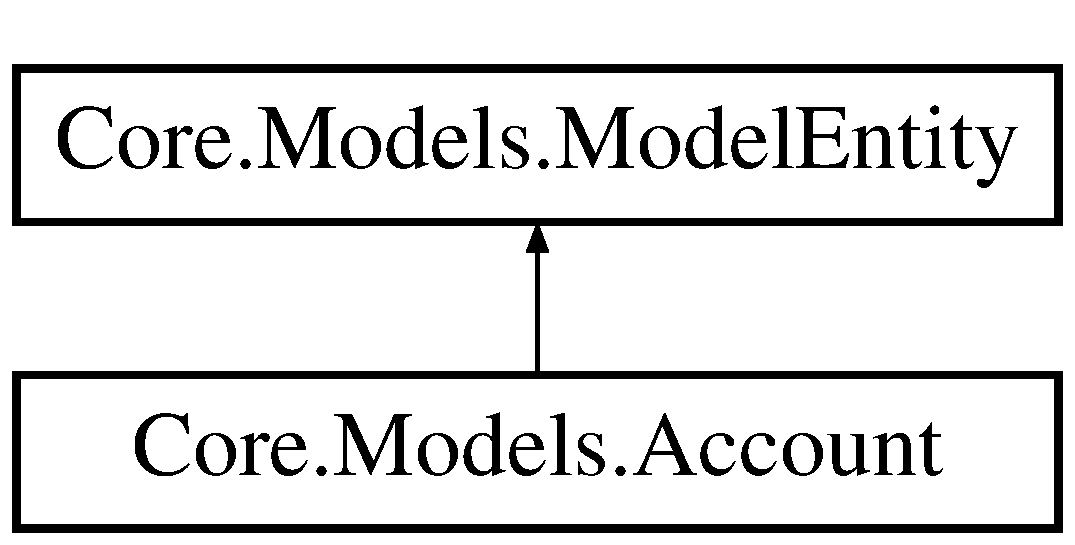
\includegraphics[height=2.000000cm]{classCore_1_1Models_1_1Account}
\end{center}
\end{figure}
\subsection*{Public Member Functions}
\begin{DoxyCompactItemize}
\item 
\hypertarget{classCore_1_1Models_1_1Account_a6142601e9f18c6453a95ebde6d8cfec3}{{\bfseries Account} (int id)}\label{classCore_1_1Models_1_1Account_a6142601e9f18c6453a95ebde6d8cfec3}

\item 
\hypertarget{classCore_1_1Models_1_1Account_acb6bb3a9e0def84b5f944891937eb173}{{\bfseries Account} (int id, string user\-Name)}\label{classCore_1_1Models_1_1Account_acb6bb3a9e0def84b5f944891937eb173}

\end{DoxyCompactItemize}
\subsection*{Properties}
\begin{DoxyCompactItemize}
\item 
\hypertarget{classCore_1_1Models_1_1Account_a7d03d99ad8aef36cd306111624ee9664}{int {\bfseries I\-D}\hspace{0.3cm}{\ttfamily  \mbox{[}get, set\mbox{]}}}\label{classCore_1_1Models_1_1Account_a7d03d99ad8aef36cd306111624ee9664}

\item 
\hypertarget{classCore_1_1Models_1_1Account_a1ffe9e8e0cfd0a45234e457a39c2de0f}{string {\bfseries User\-Name}\hspace{0.3cm}{\ttfamily  \mbox{[}get, set\mbox{]}}}\label{classCore_1_1Models_1_1Account_a1ffe9e8e0cfd0a45234e457a39c2de0f}

\item 
\hypertarget{classCore_1_1Models_1_1Account_a16db715a6cb365cc3075ba8c2c24f402}{Linked\-List$<$ \hyperlink{classCore_1_1Models_1_1PositionI}{Position\-I} $>$ {\bfseries Headquarters}\hspace{0.3cm}{\ttfamily  \mbox{[}get, set\mbox{]}}}\label{classCore_1_1Models_1_1Account_a16db715a6cb365cc3075ba8c2c24f402}

\item 
\hypertarget{classCore_1_1Models_1_1Account_a474b556453f43f821b4b3c79401288ac}{Linked\-List$<$ \hyperlink{classCore_1_1Models_1_1PositionI}{Position\-I} $>$ {\bfseries Units}\hspace{0.3cm}{\ttfamily  \mbox{[}get, set\mbox{]}}}\label{classCore_1_1Models_1_1Account_a474b556453f43f821b4b3c79401288ac}

\item 
\hypertarget{classCore_1_1Models_1_1Account_a19c8dc728a99221a064867333f8555f6}{Linked\-List$<$ \hyperlink{classCore_1_1Models_1_1PositionI}{Position\-I} $>$ {\bfseries Buildings}\hspace{0.3cm}{\ttfamily  \mbox{[}get, set\mbox{]}}}\label{classCore_1_1Models_1_1Account_a19c8dc728a99221a064867333f8555f6}

\end{DoxyCompactItemize}
\subsection*{Additional Inherited Members}


The documentation for this class was generated from the following file\-:\begin{DoxyCompactItemize}
\item 
base/\-Models/Account.\-cs\end{DoxyCompactItemize}

\hypertarget{classServer_1_1Controllers_1_1AccountController}{}\section{Server.\+Controllers.\+Account\+Controller Class Reference}
\label{classServer_1_1Controllers_1_1AccountController}\index{Server.\+Controllers.\+Account\+Controller@{Server.\+Controllers.\+Account\+Controller}}


Manages an account. Which includes Login, holding password and session and the last time when each region was loaded.  


Inheritance diagram for Server.\+Controllers.\+Account\+Controller\+:\begin{figure}[H]
\begin{center}
\leavevmode
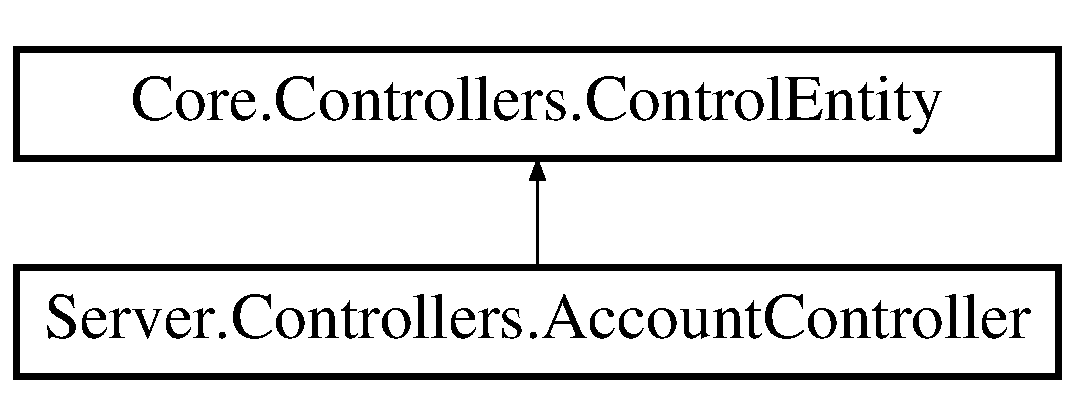
\includegraphics[height=2.000000cm]{classServer_1_1Controllers_1_1AccountController}
\end{center}
\end{figure}
\subsection*{Public Member Functions}
\begin{DoxyCompactItemize}
\item 
\hyperlink{classServer_1_1Controllers_1_1AccountController_ac35adf7e9f6d20dfbf584df2723b320c}{Account\+Controller} (\hyperlink{classCore_1_1Models_1_1Account}{Core.\+Models.\+Account} account, string password)
\begin{DoxyCompactList}\small\item\em Initializes a new instance of the \hyperlink{classServer_1_1Controllers_1_1AccountController}{Server.\+Controllers.\+Account\+Controller} class. \end{DoxyCompactList}\item 
void \hyperlink{classServer_1_1Controllers_1_1AccountController_a2326ec6c25856d4dcf65d9422b753c97}{Refresh\+Region} (\hyperlink{classCore_1_1Models_1_1RegionPosition}{Core.\+Models.\+Region\+Position} region\+Position, Date\+Time date\+Time)
\begin{DoxyCompactList}\small\item\em Every time the client is loading a region, this function should be called with the date time of the last action of the region. So it is known which data version the client has. \end{DoxyCompactList}\item 
Date\+Time \hyperlink{classServer_1_1Controllers_1_1AccountController_ae318dc148368d8a293c7fdf6dabceab6}{Get\+Region\+Status} (\hyperlink{classCore_1_1Models_1_1RegionPosition}{Core.\+Models.\+Region\+Position} region\+Position)
\begin{DoxyCompactList}\small\item\em Returns the Date\+Time of the specific region, when the last status was transferred. \end{DoxyCompactList}\item 
bool \hyperlink{classServer_1_1Controllers_1_1AccountController_a73d7223e39a37a1adfb3b04ab7513031}{Login} (string username, string password)
\begin{DoxyCompactList}\small\item\em Tries to login the user, return true if everything worked. \end{DoxyCompactList}\end{DoxyCompactItemize}
\subsection*{Properties}
\begin{DoxyCompactItemize}
\item 
Guid \hyperlink{classServer_1_1Controllers_1_1AccountController_a243d08e18b7e88f0ed33f3283aaf5709}{Session\+I\+D}\hspace{0.3cm}{\ttfamily  \mbox{[}get\mbox{]}}
\begin{DoxyCompactList}\small\item\em Gets the session I\+D. \end{DoxyCompactList}\end{DoxyCompactItemize}


\subsection{Detailed Description}
Manages an account. Which includes Login, holding password and session and the last time when each region was loaded. 



\subsection{Constructor \& Destructor Documentation}
\hypertarget{classServer_1_1Controllers_1_1AccountController_ac35adf7e9f6d20dfbf584df2723b320c}{}\index{Server\+::\+Controllers\+::\+Account\+Controller@{Server\+::\+Controllers\+::\+Account\+Controller}!Account\+Controller@{Account\+Controller}}
\index{Account\+Controller@{Account\+Controller}!Server\+::\+Controllers\+::\+Account\+Controller@{Server\+::\+Controllers\+::\+Account\+Controller}}
\subsubsection[{Account\+Controller(\+Core.\+Models.\+Account account, string password)}]{\setlength{\rightskip}{0pt plus 5cm}Server.\+Controllers.\+Account\+Controller.\+Account\+Controller (
\begin{DoxyParamCaption}
\item[{{\bf Core.\+Models.\+Account}}]{account, }
\item[{string}]{password}
\end{DoxyParamCaption}
)}\label{classServer_1_1Controllers_1_1AccountController_ac35adf7e9f6d20dfbf584df2723b320c}


Initializes a new instance of the \hyperlink{classServer_1_1Controllers_1_1AccountController}{Server.\+Controllers.\+Account\+Controller} class. 


\begin{DoxyParams}{Parameters}
{\em account} & User Account.\\
\hline
{\em password} & User Password.\\
\hline
\end{DoxyParams}


\subsection{Member Function Documentation}
\hypertarget{classServer_1_1Controllers_1_1AccountController_ae318dc148368d8a293c7fdf6dabceab6}{}\index{Server\+::\+Controllers\+::\+Account\+Controller@{Server\+::\+Controllers\+::\+Account\+Controller}!Get\+Region\+Status@{Get\+Region\+Status}}
\index{Get\+Region\+Status@{Get\+Region\+Status}!Server\+::\+Controllers\+::\+Account\+Controller@{Server\+::\+Controllers\+::\+Account\+Controller}}
\subsubsection[{Get\+Region\+Status(\+Core.\+Models.\+Region\+Position region\+Position)}]{\setlength{\rightskip}{0pt plus 5cm}Date\+Time Server.\+Controllers.\+Account\+Controller.\+Get\+Region\+Status (
\begin{DoxyParamCaption}
\item[{{\bf Core.\+Models.\+Region\+Position}}]{region\+Position}
\end{DoxyParamCaption}
)}\label{classServer_1_1Controllers_1_1AccountController_ae318dc148368d8a293c7fdf6dabceab6}


Returns the Date\+Time of the specific region, when the last status was transferred. 

\begin{DoxyReturn}{Returns}
A Date\+Time when the last action of a specific region was transferred. {\bfseries null} if it wasn\textquotesingle{}t loaded before.
\end{DoxyReturn}

\begin{DoxyParams}{Parameters}
{\em region\+Position} & Region Position.\\
\hline
\end{DoxyParams}
\hypertarget{classServer_1_1Controllers_1_1AccountController_a73d7223e39a37a1adfb3b04ab7513031}{}\index{Server\+::\+Controllers\+::\+Account\+Controller@{Server\+::\+Controllers\+::\+Account\+Controller}!Login@{Login}}
\index{Login@{Login}!Server\+::\+Controllers\+::\+Account\+Controller@{Server\+::\+Controllers\+::\+Account\+Controller}}
\subsubsection[{Login(string username, string password)}]{\setlength{\rightskip}{0pt plus 5cm}bool Server.\+Controllers.\+Account\+Controller.\+Login (
\begin{DoxyParamCaption}
\item[{string}]{username, }
\item[{string}]{password}
\end{DoxyParamCaption}
)}\label{classServer_1_1Controllers_1_1AccountController_a73d7223e39a37a1adfb3b04ab7513031}


Tries to login the user, return true if everything worked. 


\begin{DoxyParams}{Parameters}
{\em username} & Account Username\\
\hline
{\em password} & Account Password\\
\hline
\end{DoxyParams}
\hypertarget{classServer_1_1Controllers_1_1AccountController_a2326ec6c25856d4dcf65d9422b753c97}{}\index{Server\+::\+Controllers\+::\+Account\+Controller@{Server\+::\+Controllers\+::\+Account\+Controller}!Refresh\+Region@{Refresh\+Region}}
\index{Refresh\+Region@{Refresh\+Region}!Server\+::\+Controllers\+::\+Account\+Controller@{Server\+::\+Controllers\+::\+Account\+Controller}}
\subsubsection[{Refresh\+Region(\+Core.\+Models.\+Region\+Position region\+Position, Date\+Time date\+Time)}]{\setlength{\rightskip}{0pt plus 5cm}void Server.\+Controllers.\+Account\+Controller.\+Refresh\+Region (
\begin{DoxyParamCaption}
\item[{{\bf Core.\+Models.\+Region\+Position}}]{region\+Position, }
\item[{Date\+Time}]{date\+Time}
\end{DoxyParamCaption}
)}\label{classServer_1_1Controllers_1_1AccountController_a2326ec6c25856d4dcf65d9422b753c97}


Every time the client is loading a region, this function should be called with the date time of the last action of the region. So it is known which data version the client has. 


\begin{DoxyParams}{Parameters}
{\em region\+Position} & Region position.\\
\hline
{\em date\+Time} & Date time.\\
\hline
\end{DoxyParams}


\subsection{Property Documentation}
\hypertarget{classServer_1_1Controllers_1_1AccountController_a243d08e18b7e88f0ed33f3283aaf5709}{}\index{Server\+::\+Controllers\+::\+Account\+Controller@{Server\+::\+Controllers\+::\+Account\+Controller}!Session\+I\+D@{Session\+I\+D}}
\index{Session\+I\+D@{Session\+I\+D}!Server\+::\+Controllers\+::\+Account\+Controller@{Server\+::\+Controllers\+::\+Account\+Controller}}
\subsubsection[{Session\+I\+D}]{\setlength{\rightskip}{0pt plus 5cm}Guid Server.\+Controllers.\+Account\+Controller.\+Session\+I\+D\hspace{0.3cm}{\ttfamily [get]}}\label{classServer_1_1Controllers_1_1AccountController_a243d08e18b7e88f0ed33f3283aaf5709}


Gets the session I\+D. 

The session I\+D.

The documentation for this class was generated from the following file\+:\begin{DoxyCompactItemize}
\item 
tcpserver/\+Controllers/Account\+Controller.\+cs\end{DoxyCompactItemize}

\hypertarget{classCore_1_1Models_1_1AccountManager}{\section{Core.\-Models.\-Account\-Manager Class Reference}
\label{classCore_1_1Models_1_1AccountManager}\index{Core.\-Models.\-Account\-Manager@{Core.\-Models.\-Account\-Manager}}
}


Contains all \hyperlink{classCore_1_1Models_1_1Account}{Account} with id.  


Inheritance diagram for Core.\-Models.\-Account\-Manager\-:\begin{figure}[H]
\begin{center}
\leavevmode
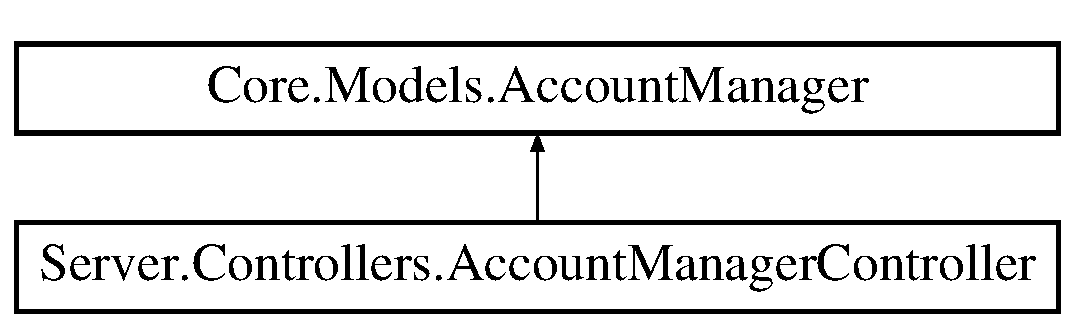
\includegraphics[height=2.000000cm]{classCore_1_1Models_1_1AccountManager}
\end{center}
\end{figure}
\subsection*{Public Member Functions}
\begin{DoxyCompactItemize}
\item 
\hypertarget{classCore_1_1Models_1_1AccountManager_a191e85e6daf1d61bf6b0f0318c304875}{void {\bfseries Add\-Account} (\hyperlink{classCore_1_1Models_1_1Account}{Account} account)}\label{classCore_1_1Models_1_1AccountManager_a191e85e6daf1d61bf6b0f0318c304875}

\item 
\hypertarget{classCore_1_1Models_1_1AccountManager_aa34df711aff2cc6588f78e6abc6e9ad2}{\hyperlink{classCore_1_1Models_1_1Account}{Account} {\bfseries Get\-Account\-Or\-Empty} (int id)}\label{classCore_1_1Models_1_1AccountManager_aa34df711aff2cc6588f78e6abc6e9ad2}

\item 
\hyperlink{classCore_1_1Models_1_1Account}{Account} \hyperlink{classCore_1_1Models_1_1AccountManager_a0a85126c3cd1a3ceeb6ceb08f0d817cb}{Get\-Account} (int id)
\begin{DoxyCompactList}\small\item\em Returns the account \end{DoxyCompactList}\end{DoxyCompactItemize}
\subsection*{Public Attributes}
\begin{DoxyCompactItemize}
\item 
\hypertarget{classCore_1_1Models_1_1AccountManager_ac5ed7a3991ca4db781a9befdbc731e6d}{Concurrent\-Dictionary$<$ int, \\*
\hyperlink{classCore_1_1Models_1_1Account}{Account} $>$ {\bfseries Accounts}}\label{classCore_1_1Models_1_1AccountManager_ac5ed7a3991ca4db781a9befdbc731e6d}

\end{DoxyCompactItemize}


\subsection{Detailed Description}
Contains all \hyperlink{classCore_1_1Models_1_1Account}{Account} with id. 



\subsection{Member Function Documentation}
\hypertarget{classCore_1_1Models_1_1AccountManager_a0a85126c3cd1a3ceeb6ceb08f0d817cb}{\index{Core\-::\-Models\-::\-Account\-Manager@{Core\-::\-Models\-::\-Account\-Manager}!Get\-Account@{Get\-Account}}
\index{Get\-Account@{Get\-Account}!Core::Models::AccountManager@{Core\-::\-Models\-::\-Account\-Manager}}
\subsubsection[{Get\-Account}]{\setlength{\rightskip}{0pt plus 5cm}{\bf Account} Core.\-Models.\-Account\-Manager.\-Get\-Account (
\begin{DoxyParamCaption}
\item[{int}]{id}
\end{DoxyParamCaption}
)\hspace{0.3cm}{\ttfamily [inline]}}}\label{classCore_1_1Models_1_1AccountManager_a0a85126c3cd1a3ceeb6ceb08f0d817cb}


Returns the account 

\begin{DoxyReturn}{Returns}
The account or null (if there is none)
\end{DoxyReturn}

\begin{DoxyParams}{Parameters}
{\em id} & Identifier.\\
\hline
\end{DoxyParams}


The documentation for this class was generated from the following file\-:\begin{DoxyCompactItemize}
\item 
base/\-Models/\-Manager/Account\-Manager.\-cs\end{DoxyCompactItemize}

\hypertarget{classServer_1_1Controllers_1_1AccountManagerController}{\section{Server.\-Controllers.\-Account\-Manager\-Controller Class Reference}
\label{classServer_1_1Controllers_1_1AccountManagerController}\index{Server.\-Controllers.\-Account\-Manager\-Controller@{Server.\-Controllers.\-Account\-Manager\-Controller}}
}


The \hyperlink{classServer_1_1Controllers_1_1AccountManagerController}{Account\-Manager\-Controller} handles a list of all users and those, which are logged in. It can also log in users and verify a session id.  


Inheritance diagram for Server.\-Controllers.\-Account\-Manager\-Controller\-:\begin{figure}[H]
\begin{center}
\leavevmode
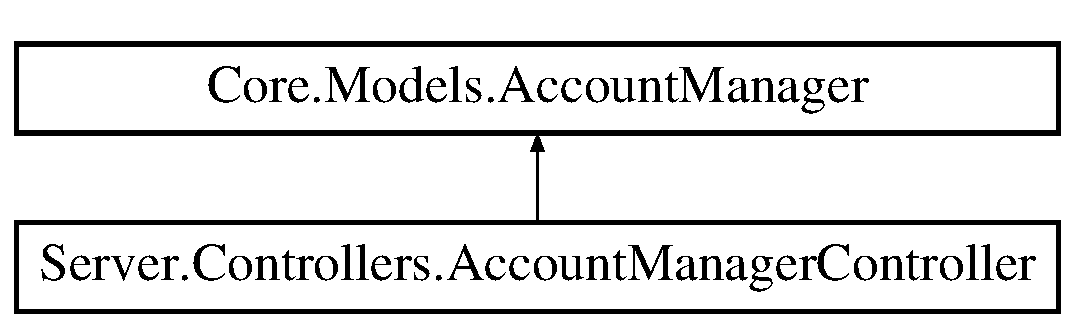
\includegraphics[height=2.000000cm]{classServer_1_1Controllers_1_1AccountManagerController}
\end{center}
\end{figure}
\subsection*{Public Member Functions}
\begin{DoxyCompactItemize}
\item 
\hyperlink{classCore_1_1Models_1_1Account}{Account} \hyperlink{classServer_1_1Controllers_1_1AccountManagerController_ae290a06ee465aca4b38a7cd61c304a26}{Login} (string username, string password)
\begin{DoxyCompactList}\small\item\em Login with a username und password, returns Account if everything worked, otherwise {\bfseries null} \end{DoxyCompactList}\item 
\hyperlink{classCore_1_1Models_1_1Account}{Account} \hyperlink{classServer_1_1Controllers_1_1AccountManagerController_aa78f40e7fdfcc38730c4fe118b52b5eb}{Registrate} (string username, string password)
\begin{DoxyCompactList}\small\item\em Registrates the username/password combination as a new user. If the username already exist, he will be logged in. returns {\bfseries null} when username is already taken with an different password. \end{DoxyCompactList}\item 
\hyperlink{classCore_1_1Models_1_1Account}{Account} \hyperlink{classServer_1_1Controllers_1_1AccountManagerController_afd9fd2cdd749a94178834540c91ceef4}{Get\-Account\-By\-Session} (Guid session\-I\-D)
\begin{DoxyCompactList}\small\item\em Gets the account by a session. \end{DoxyCompactList}\end{DoxyCompactItemize}
\subsection*{Additional Inherited Members}


\subsection{Detailed Description}
The \hyperlink{classServer_1_1Controllers_1_1AccountManagerController}{Account\-Manager\-Controller} handles a list of all users and those, which are logged in. It can also log in users and verify a session id. 



\subsection{Member Function Documentation}
\hypertarget{classServer_1_1Controllers_1_1AccountManagerController_afd9fd2cdd749a94178834540c91ceef4}{\index{Server\-::\-Controllers\-::\-Account\-Manager\-Controller@{Server\-::\-Controllers\-::\-Account\-Manager\-Controller}!Get\-Account\-By\-Session@{Get\-Account\-By\-Session}}
\index{Get\-Account\-By\-Session@{Get\-Account\-By\-Session}!Server::Controllers::AccountManagerController@{Server\-::\-Controllers\-::\-Account\-Manager\-Controller}}
\subsubsection[{Get\-Account\-By\-Session}]{\setlength{\rightskip}{0pt plus 5cm}{\bf Account} Server.\-Controllers.\-Account\-Manager\-Controller.\-Get\-Account\-By\-Session (
\begin{DoxyParamCaption}
\item[{Guid}]{session\-I\-D}
\end{DoxyParamCaption}
)\hspace{0.3cm}{\ttfamily [inline]}}}\label{classServer_1_1Controllers_1_1AccountManagerController_afd9fd2cdd749a94178834540c91ceef4}


Gets the account by a session. 

\begin{DoxyReturn}{Returns}
An Account which is assigned to this session id or null, if there was none.
\end{DoxyReturn}

\begin{DoxyParams}{Parameters}
{\em session\-I\-D} & Session I\-D\\
\hline
\end{DoxyParams}
\hypertarget{classServer_1_1Controllers_1_1AccountManagerController_ae290a06ee465aca4b38a7cd61c304a26}{\index{Server\-::\-Controllers\-::\-Account\-Manager\-Controller@{Server\-::\-Controllers\-::\-Account\-Manager\-Controller}!Login@{Login}}
\index{Login@{Login}!Server::Controllers::AccountManagerController@{Server\-::\-Controllers\-::\-Account\-Manager\-Controller}}
\subsubsection[{Login}]{\setlength{\rightskip}{0pt plus 5cm}{\bf Account} Server.\-Controllers.\-Account\-Manager\-Controller.\-Login (
\begin{DoxyParamCaption}
\item[{string}]{username, }
\item[{string}]{password}
\end{DoxyParamCaption}
)\hspace{0.3cm}{\ttfamily [inline]}}}\label{classServer_1_1Controllers_1_1AccountManagerController_ae290a06ee465aca4b38a7cd61c304a26}


Login with a username und password, returns Account if everything worked, otherwise {\bfseries null} 


\begin{DoxyParams}{Parameters}
{\em username} & Username.\\
\hline
{\em password} & Password.\\
\hline
\end{DoxyParams}
\hypertarget{classServer_1_1Controllers_1_1AccountManagerController_aa78f40e7fdfcc38730c4fe118b52b5eb}{\index{Server\-::\-Controllers\-::\-Account\-Manager\-Controller@{Server\-::\-Controllers\-::\-Account\-Manager\-Controller}!Registrate@{Registrate}}
\index{Registrate@{Registrate}!Server::Controllers::AccountManagerController@{Server\-::\-Controllers\-::\-Account\-Manager\-Controller}}
\subsubsection[{Registrate}]{\setlength{\rightskip}{0pt plus 5cm}{\bf Account} Server.\-Controllers.\-Account\-Manager\-Controller.\-Registrate (
\begin{DoxyParamCaption}
\item[{string}]{username, }
\item[{string}]{password}
\end{DoxyParamCaption}
)\hspace{0.3cm}{\ttfamily [inline]}}}\label{classServer_1_1Controllers_1_1AccountManagerController_aa78f40e7fdfcc38730c4fe118b52b5eb}


Registrates the username/password combination as a new user. If the username already exist, he will be logged in. returns {\bfseries null} when username is already taken with an different password. 


\begin{DoxyParams}{Parameters}
{\em username} & Username.\\
\hline
{\em password} & Password.\\
\hline
\end{DoxyParams}


The documentation for this class was generated from the following file\-:\begin{DoxyCompactItemize}
\item 
server/\-Controllers/Account\-Manager\-Controller.\-cs\end{DoxyCompactItemize}

\hypertarget{classCore_1_1Controllers_1_1Actions_1_1Action}{}\section{Core.\+Controllers.\+Actions.\+Action Class Reference}
\label{classCore_1_1Controllers_1_1Actions_1_1Action}\index{Core.\+Controllers.\+Actions.\+Action@{Core.\+Controllers.\+Actions.\+Action}}


\hyperlink{classCore_1_1Controllers_1_1Actions_1_1Action}{Action} class. Should be used as base for each other action. \hyperlink{namespaceCore_1_1Controllers_1_1Actions}{Actions} are part of the game logic, which can be used from the server or the client to manipulate the world. Every action should do deterministic calculations, so the client can calculate the current game state by an old game state and the list of actions which were executed since the last loaded game state.  


Inheritance diagram for Core.\+Controllers.\+Actions.\+Action\+:\begin{figure}[H]
\begin{center}
\leavevmode
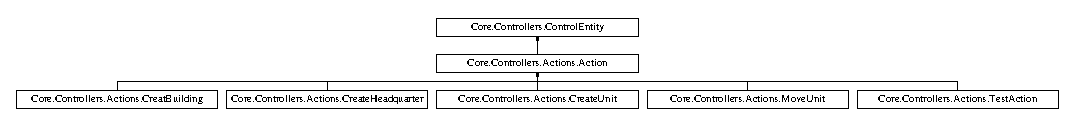
\includegraphics[height=1.418919cm]{classCore_1_1Controllers_1_1Actions_1_1Action}
\end{center}
\end{figure}
\subsection*{Public Member Functions}
\begin{DoxyCompactItemize}
\item 
\hyperlink{classCore_1_1Controllers_1_1Actions_1_1Action_abb5103ff9280d2556e57a0fdaf090fe1}{Action} (\hyperlink{classCore_1_1Models_1_1ModelEntity}{Core.\+Models.\+Model\+Entity} model)
\begin{DoxyCompactList}\small\item\em Initializes a new instance of the \hyperlink{classCore_1_1Controllers_1_1Actions_1_1Action}{Core.\+Controllers.\+Actions.\+Action} class. \end{DoxyCompactList}\item 
virtual Concurrent\+Bag$<$ \hyperlink{classCore_1_1Models_1_1Region}{Core.\+Models.\+Region} $>$ \hyperlink{classCore_1_1Controllers_1_1Actions_1_1Action_aa11bdeffff43ec47ac7c3d6843a85674}{Get\+Affected\+Regions} ()
\begin{DoxyCompactList}\small\item\em Returns a bag of all regions which could be affected by this action. \end{DoxyCompactList}\item 
virtual \hyperlink{classCore_1_1Models_1_1RegionPosition}{Core.\+Models.\+Region\+Position} \hyperlink{classCore_1_1Controllers_1_1Actions_1_1Action_a6ffe3c30cb5648a81f50096f4f332d5a}{Get\+Region\+Position} ()
\begin{DoxyCompactList}\small\item\em Returns the Position where the action should be executed (e.\+g. first region) \end{DoxyCompactList}\item 
virtual bool \hyperlink{classCore_1_1Controllers_1_1Actions_1_1Action_a405b995343a9394ad19e05a699a4e6d9}{Possible} ()
\begin{DoxyCompactList}\small\item\em Returns if the action is even possible. \end{DoxyCompactList}\item 
virtual Concurrent\+Bag$<$ \hyperlink{classCore_1_1Models_1_1Region}{Core.\+Models.\+Region} $>$ \hyperlink{classCore_1_1Controllers_1_1Actions_1_1Action_afbb091ee28eee896951fac600188d446}{Do} ()
\begin{DoxyCompactList}\small\item\em Apply action-\/related changes to the world. Returns set of changed Regions if everything worked, otherwise null \end{DoxyCompactList}\item 
virtual bool \hyperlink{classCore_1_1Controllers_1_1Actions_1_1Action_ada4c77dfeee78ded10a6eb6a506defb4}{Catch} ()
\begin{DoxyCompactList}\small\item\em If an error occurred in do, this function will be called to set the data to the last known valid state. \end{DoxyCompactList}\end{DoxyCompactItemize}
\subsection*{Additional Inherited Members}


\subsection{Detailed Description}
\hyperlink{classCore_1_1Controllers_1_1Actions_1_1Action}{Action} class. Should be used as base for each other action. \hyperlink{namespaceCore_1_1Controllers_1_1Actions}{Actions} are part of the game logic, which can be used from the server or the client to manipulate the world. Every action should do deterministic calculations, so the client can calculate the current game state by an old game state and the list of actions which were executed since the last loaded game state. 



\subsection{Constructor \& Destructor Documentation}
\hypertarget{classCore_1_1Controllers_1_1Actions_1_1Action_abb5103ff9280d2556e57a0fdaf090fe1}{}\index{Core\+::\+Controllers\+::\+Actions\+::\+Action@{Core\+::\+Controllers\+::\+Actions\+::\+Action}!Action@{Action}}
\index{Action@{Action}!Core\+::\+Controllers\+::\+Actions\+::\+Action@{Core\+::\+Controllers\+::\+Actions\+::\+Action}}
\subsubsection[{Action(\+Core.\+Models.\+Model\+Entity model)}]{\setlength{\rightskip}{0pt plus 5cm}Core.\+Controllers.\+Actions.\+Action.\+Action (
\begin{DoxyParamCaption}
\item[{{\bf Core.\+Models.\+Model\+Entity}}]{model}
\end{DoxyParamCaption}
)}\label{classCore_1_1Controllers_1_1Actions_1_1Action_abb5103ff9280d2556e57a0fdaf090fe1}


Initializes a new instance of the \hyperlink{classCore_1_1Controllers_1_1Actions_1_1Action}{Core.\+Controllers.\+Actions.\+Action} class. 


\begin{DoxyParams}{Parameters}
{\em model} & action model.\\
\hline
\end{DoxyParams}


\subsection{Member Function Documentation}
\hypertarget{classCore_1_1Controllers_1_1Actions_1_1Action_ada4c77dfeee78ded10a6eb6a506defb4}{}\index{Core\+::\+Controllers\+::\+Actions\+::\+Action@{Core\+::\+Controllers\+::\+Actions\+::\+Action}!Catch@{Catch}}
\index{Catch@{Catch}!Core\+::\+Controllers\+::\+Actions\+::\+Action@{Core\+::\+Controllers\+::\+Actions\+::\+Action}}
\subsubsection[{Catch()}]{\setlength{\rightskip}{0pt plus 5cm}virtual bool Core.\+Controllers.\+Actions.\+Action.\+Catch (
\begin{DoxyParamCaption}
{}
\end{DoxyParamCaption}
)\hspace{0.3cm}{\ttfamily [virtual]}}\label{classCore_1_1Controllers_1_1Actions_1_1Action_ada4c77dfeee78ded10a6eb6a506defb4}


If an error occurred in do, this function will be called to set the data to the last known valid state. 

\begin{DoxyReturn}{Returns}
true if rewind was successfully
\end{DoxyReturn}


Reimplemented in \hyperlink{classCore_1_1Controllers_1_1Actions_1_1MoveUnit_a80ff3497561ed98a933e41f48830d947}{Core.\+Controllers.\+Actions.\+Move\+Unit}, \hyperlink{classCore_1_1Controllers_1_1Actions_1_1CreateTerritoryBuilding_a07c2b5afe31a65bea350ff31e39508b4}{Core.\+Controllers.\+Actions.\+Create\+Territory\+Building}, \hyperlink{classCore_1_1Controllers_1_1Actions_1_1CreateUnit_ac2763a79e6767ac7c5179281cb4e0a6f}{Core.\+Controllers.\+Actions.\+Create\+Unit}, and \hyperlink{classCore_1_1Controllers_1_1Actions_1_1CreateBuilding_ad63ea1b154c0f04d79ed9a6316d41382}{Core.\+Controllers.\+Actions.\+Create\+Building}.

\hypertarget{classCore_1_1Controllers_1_1Actions_1_1Action_afbb091ee28eee896951fac600188d446}{}\index{Core\+::\+Controllers\+::\+Actions\+::\+Action@{Core\+::\+Controllers\+::\+Actions\+::\+Action}!Do@{Do}}
\index{Do@{Do}!Core\+::\+Controllers\+::\+Actions\+::\+Action@{Core\+::\+Controllers\+::\+Actions\+::\+Action}}
\subsubsection[{Do()}]{\setlength{\rightskip}{0pt plus 5cm}virtual Concurrent\+Bag$<${\bf Core.\+Models.\+Region}$>$ Core.\+Controllers.\+Actions.\+Action.\+Do (
\begin{DoxyParamCaption}
{}
\end{DoxyParamCaption}
)\hspace{0.3cm}{\ttfamily [virtual]}}\label{classCore_1_1Controllers_1_1Actions_1_1Action_afbb091ee28eee896951fac600188d446}


Apply action-\/related changes to the world. Returns set of changed Regions if everything worked, otherwise null 

\begin{DoxyReturn}{Returns}
all affected (changed) regions
\end{DoxyReturn}


Reimplemented in \hyperlink{classCore_1_1Controllers_1_1Actions_1_1CreateTerritoryBuilding_a3cda553c756ebbe5170a477576e73c03}{Core.\+Controllers.\+Actions.\+Create\+Territory\+Building}, \hyperlink{classCore_1_1Controllers_1_1Actions_1_1MoveUnit_adaf6b91a2e858d8805ea8ed83947b27a}{Core.\+Controllers.\+Actions.\+Move\+Unit}, \hyperlink{classCore_1_1Controllers_1_1Actions_1_1CreateUnit_a0afdf65e7e04f108bb257eae3327eac0}{Core.\+Controllers.\+Actions.\+Create\+Unit}, and \hyperlink{classCore_1_1Controllers_1_1Actions_1_1CreateBuilding_a6f640077d26410e8ea891b7300654c61}{Core.\+Controllers.\+Actions.\+Create\+Building}.

\hypertarget{classCore_1_1Controllers_1_1Actions_1_1Action_aa11bdeffff43ec47ac7c3d6843a85674}{}\index{Core\+::\+Controllers\+::\+Actions\+::\+Action@{Core\+::\+Controllers\+::\+Actions\+::\+Action}!Get\+Affected\+Regions@{Get\+Affected\+Regions}}
\index{Get\+Affected\+Regions@{Get\+Affected\+Regions}!Core\+::\+Controllers\+::\+Actions\+::\+Action@{Core\+::\+Controllers\+::\+Actions\+::\+Action}}
\subsubsection[{Get\+Affected\+Regions()}]{\setlength{\rightskip}{0pt plus 5cm}virtual Concurrent\+Bag$<${\bf Core.\+Models.\+Region}$>$ Core.\+Controllers.\+Actions.\+Action.\+Get\+Affected\+Regions (
\begin{DoxyParamCaption}
{}
\end{DoxyParamCaption}
)\hspace{0.3cm}{\ttfamily [virtual]}}\label{classCore_1_1Controllers_1_1Actions_1_1Action_aa11bdeffff43ec47ac7c3d6843a85674}


Returns a bag of all regions which could be affected by this action. 

\begin{DoxyReturn}{Returns}
The affected regions.
\end{DoxyReturn}


Reimplemented in \hyperlink{classCore_1_1Controllers_1_1Actions_1_1MoveUnit_a0331c4888d9efc148ecc501b4db37481}{Core.\+Controllers.\+Actions.\+Move\+Unit}, \hyperlink{classCore_1_1Controllers_1_1Actions_1_1CreateBuilding_a456e8ed7d1da08bd5da0baf58600a227}{Core.\+Controllers.\+Actions.\+Create\+Building}, \hyperlink{classCore_1_1Controllers_1_1Actions_1_1CreateUnit_a740be9051fcd4f9a8e22d702da400ba7}{Core.\+Controllers.\+Actions.\+Create\+Unit}, and \hyperlink{classCore_1_1Controllers_1_1Actions_1_1CreateTerritoryBuilding_a7bb58b17239efcaa57968cee96b77bb8}{Core.\+Controllers.\+Actions.\+Create\+Territory\+Building}.

\hypertarget{classCore_1_1Controllers_1_1Actions_1_1Action_a6ffe3c30cb5648a81f50096f4f332d5a}{}\index{Core\+::\+Controllers\+::\+Actions\+::\+Action@{Core\+::\+Controllers\+::\+Actions\+::\+Action}!Get\+Region\+Position@{Get\+Region\+Position}}
\index{Get\+Region\+Position@{Get\+Region\+Position}!Core\+::\+Controllers\+::\+Actions\+::\+Action@{Core\+::\+Controllers\+::\+Actions\+::\+Action}}
\subsubsection[{Get\+Region\+Position()}]{\setlength{\rightskip}{0pt plus 5cm}virtual {\bf Core.\+Models.\+Region\+Position} Core.\+Controllers.\+Actions.\+Action.\+Get\+Region\+Position (
\begin{DoxyParamCaption}
{}
\end{DoxyParamCaption}
)\hspace{0.3cm}{\ttfamily [virtual]}}\label{classCore_1_1Controllers_1_1Actions_1_1Action_a6ffe3c30cb5648a81f50096f4f332d5a}


Returns the Position where the action should be executed (e.\+g. first region) 

\begin{DoxyReturn}{Returns}
\hyperlink{classCore_1_1Controllers_1_1Actions_1_1Action}{Action} execution Region\+Position.
\end{DoxyReturn}


Reimplemented in \hyperlink{classCore_1_1Controllers_1_1Actions_1_1MoveUnit_a87a9c5589011c8e86770e1b1be487381}{Core.\+Controllers.\+Actions.\+Move\+Unit}, \hyperlink{classCore_1_1Controllers_1_1Actions_1_1CreateTerritoryBuilding_a293d75e2f559ce6c456601e030597b85}{Core.\+Controllers.\+Actions.\+Create\+Territory\+Building}, \hyperlink{classCore_1_1Controllers_1_1Actions_1_1CreateUnit_a04a85d0db9c84ca3f0e97049cca4f9c0}{Core.\+Controllers.\+Actions.\+Create\+Unit}, and \hyperlink{classCore_1_1Controllers_1_1Actions_1_1CreateBuilding_a65ab8070b1fd436ee2f48c2c84b9ff57}{Core.\+Controllers.\+Actions.\+Create\+Building}.

\hypertarget{classCore_1_1Controllers_1_1Actions_1_1Action_a405b995343a9394ad19e05a699a4e6d9}{}\index{Core\+::\+Controllers\+::\+Actions\+::\+Action@{Core\+::\+Controllers\+::\+Actions\+::\+Action}!Possible@{Possible}}
\index{Possible@{Possible}!Core\+::\+Controllers\+::\+Actions\+::\+Action@{Core\+::\+Controllers\+::\+Actions\+::\+Action}}
\subsubsection[{Possible()}]{\setlength{\rightskip}{0pt plus 5cm}virtual bool Core.\+Controllers.\+Actions.\+Action.\+Possible (
\begin{DoxyParamCaption}
{}
\end{DoxyParamCaption}
)\hspace{0.3cm}{\ttfamily [virtual]}}\label{classCore_1_1Controllers_1_1Actions_1_1Action_a405b995343a9394ad19e05a699a4e6d9}


Returns if the action is even possible. 

\begin{DoxyReturn}{Returns}
true if this is action possible
\end{DoxyReturn}


Reimplemented in \hyperlink{classCore_1_1Controllers_1_1Actions_1_1MoveUnit_a6689af13f9a2f8ff90ad72d2ac327a52}{Core.\+Controllers.\+Actions.\+Move\+Unit}, \hyperlink{classCore_1_1Controllers_1_1Actions_1_1CreateUnit_a30ceafb2aa0fb1b801a8abd659c9d70f}{Core.\+Controllers.\+Actions.\+Create\+Unit}, \hyperlink{classCore_1_1Controllers_1_1Actions_1_1CreateTerritoryBuilding_a972f538b1c4a17240b6d7f9d7e0b2662}{Core.\+Controllers.\+Actions.\+Create\+Territory\+Building}, and \hyperlink{classCore_1_1Controllers_1_1Actions_1_1CreateBuilding_a254e5f630e31046dfb9bdc5e8b25d7d9}{Core.\+Controllers.\+Actions.\+Create\+Building}.



The documentation for this class was generated from the following file\+:\begin{DoxyCompactItemize}
\item 
base/\+Controllers/\+Actions/Action.\+cs\end{DoxyCompactItemize}

\hypertarget{classClient_1_1Common_1_1Views_1_1Actions_1_1Action}{}\section{Client.\+Common.\+Views.\+Actions.\+Action Class Reference}
\label{classClient_1_1Common_1_1Views_1_1Actions_1_1Action}\index{Client.\+Common.\+Views.\+Actions.\+Action@{Client.\+Common.\+Views.\+Actions.\+Action}}


The View part of the \hyperlink{namespaceClient_1_1Common_1_1Views_1_1Actions}{Actions}. So an action can be displayed.  


Inheritance diagram for Client.\+Common.\+Views.\+Actions.\+Action\+:\begin{figure}[H]
\begin{center}
\leavevmode
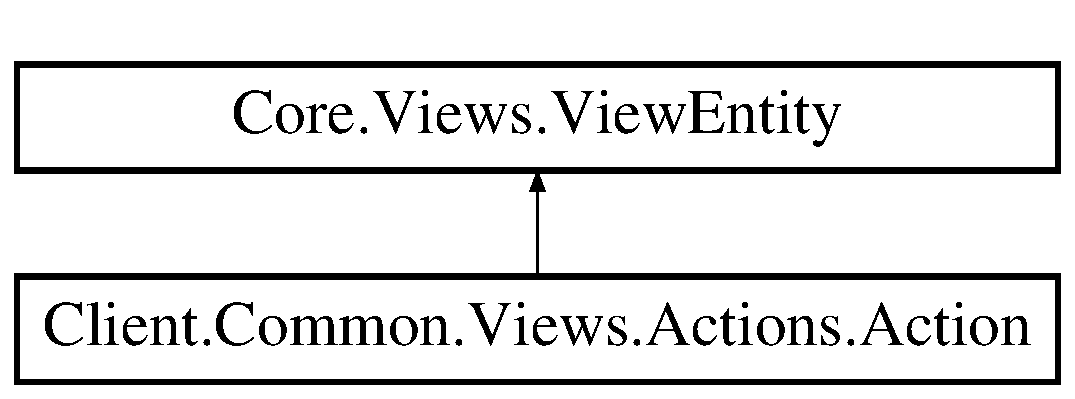
\includegraphics[height=2.000000cm]{classClient_1_1Common_1_1Views_1_1Actions_1_1Action}
\end{center}
\end{figure}
\subsection*{Public Member Functions}
\begin{DoxyCompactItemize}
\item 
\hyperlink{classClient_1_1Common_1_1Views_1_1Actions_1_1Action_ae6ccd18f995bf709877f508c65308c42}{Action} (\hyperlink{classCore_1_1Models_1_1ModelEntity}{Core.\+Models.\+Model\+Entity} model)
\begin{DoxyCompactList}\small\item\em Initializes a new instance of the \hyperlink{classClient_1_1Common_1_1Views_1_1Actions_1_1Action}{Client.\+Common.\+Views.\+Actions.\+Action} class. \end{DoxyCompactList}\item 
virtual void \hyperlink{classClient_1_1Common_1_1Views_1_1Actions_1_1Action_ad129f8cb1d8079f76d8199dbc80d3c0d}{Before\+Do} ()
\begin{DoxyCompactList}\small\item\em Gets called before Action\+Control.\+Do() gets executed. Should get and store data which will be needed in Schedule. \end{DoxyCompactList}\item 
virtual bool \hyperlink{classClient_1_1Common_1_1Views_1_1Actions_1_1Action_a92fdf89fb39016ef84e08dc3c7352d51}{Schedule} (float frame\+Times\+In\+Second)
\begin{DoxyCompactList}\small\item\em Schedules the action. Should do anything do animate the action (e.\+g. draw the entity, animate his moving or start/end animating a fight) Returns true if the action has ended, otherwise false. \end{DoxyCompactList}\end{DoxyCompactItemize}
\subsection*{Additional Inherited Members}


\subsection{Detailed Description}
The View part of the \hyperlink{namespaceClient_1_1Common_1_1Views_1_1Actions}{Actions}. So an action can be displayed. 



\subsection{Constructor \& Destructor Documentation}
\hypertarget{classClient_1_1Common_1_1Views_1_1Actions_1_1Action_ae6ccd18f995bf709877f508c65308c42}{}\index{Client\+::\+Common\+::\+Views\+::\+Actions\+::\+Action@{Client\+::\+Common\+::\+Views\+::\+Actions\+::\+Action}!Action@{Action}}
\index{Action@{Action}!Client\+::\+Common\+::\+Views\+::\+Actions\+::\+Action@{Client\+::\+Common\+::\+Views\+::\+Actions\+::\+Action}}
\subsubsection[{Action(\+Core.\+Models.\+Model\+Entity model)}]{\setlength{\rightskip}{0pt plus 5cm}Client.\+Common.\+Views.\+Actions.\+Action.\+Action (
\begin{DoxyParamCaption}
\item[{{\bf Core.\+Models.\+Model\+Entity}}]{model}
\end{DoxyParamCaption}
)}\label{classClient_1_1Common_1_1Views_1_1Actions_1_1Action_ae6ccd18f995bf709877f508c65308c42}


Initializes a new instance of the \hyperlink{classClient_1_1Common_1_1Views_1_1Actions_1_1Action}{Client.\+Common.\+Views.\+Actions.\+Action} class. 


\begin{DoxyParams}{Parameters}
{\em model} & The action Model.\\
\hline
\end{DoxyParams}


\subsection{Member Function Documentation}
\hypertarget{classClient_1_1Common_1_1Views_1_1Actions_1_1Action_ad129f8cb1d8079f76d8199dbc80d3c0d}{}\index{Client\+::\+Common\+::\+Views\+::\+Actions\+::\+Action@{Client\+::\+Common\+::\+Views\+::\+Actions\+::\+Action}!Before\+Do@{Before\+Do}}
\index{Before\+Do@{Before\+Do}!Client\+::\+Common\+::\+Views\+::\+Actions\+::\+Action@{Client\+::\+Common\+::\+Views\+::\+Actions\+::\+Action}}
\subsubsection[{Before\+Do()}]{\setlength{\rightskip}{0pt plus 5cm}virtual void Client.\+Common.\+Views.\+Actions.\+Action.\+Before\+Do (
\begin{DoxyParamCaption}
{}
\end{DoxyParamCaption}
)\hspace{0.3cm}{\ttfamily [virtual]}}\label{classClient_1_1Common_1_1Views_1_1Actions_1_1Action_ad129f8cb1d8079f76d8199dbc80d3c0d}


Gets called before Action\+Control.\+Do() gets executed. Should get and store data which will be needed in Schedule. 

\hypertarget{classClient_1_1Common_1_1Views_1_1Actions_1_1Action_a92fdf89fb39016ef84e08dc3c7352d51}{}\index{Client\+::\+Common\+::\+Views\+::\+Actions\+::\+Action@{Client\+::\+Common\+::\+Views\+::\+Actions\+::\+Action}!Schedule@{Schedule}}
\index{Schedule@{Schedule}!Client\+::\+Common\+::\+Views\+::\+Actions\+::\+Action@{Client\+::\+Common\+::\+Views\+::\+Actions\+::\+Action}}
\subsubsection[{Schedule(float frame\+Times\+In\+Second)}]{\setlength{\rightskip}{0pt plus 5cm}virtual bool Client.\+Common.\+Views.\+Actions.\+Action.\+Schedule (
\begin{DoxyParamCaption}
\item[{float}]{frame\+Times\+In\+Second}
\end{DoxyParamCaption}
)\hspace{0.3cm}{\ttfamily [virtual]}}\label{classClient_1_1Common_1_1Views_1_1Actions_1_1Action_a92fdf89fb39016ef84e08dc3c7352d51}


Schedules the action. Should do anything do animate the action (e.\+g. draw the entity, animate his moving or start/end animating a fight) Returns true if the action has ended, otherwise false. 


\begin{DoxyParams}{Parameters}
{\em frame\+Times\+In\+Second} & frames times in seconds.\\
\hline
\end{DoxyParams}
\begin{DoxyReturn}{Returns}
true if the schedule of the action is done
\end{DoxyReturn}


The documentation for this class was generated from the following file\+:\begin{DoxyCompactItemize}
\item 
client/client/client.\+Common/\+Views/\+Actions/Action.\+cs\end{DoxyCompactItemize}

\hypertarget{classCore_1_1Models_1_1Action}{}\section{Core.\+Models.\+Action Class Reference}
\label{classCore_1_1Models_1_1Action}\index{Core.\+Models.\+Action@{Core.\+Models.\+Action}}


\hyperlink{classCore_1_1Models_1_1Action}{Action} model which should contains all needed data for the action control.  


Inheritance diagram for Core.\+Models.\+Action\+:\begin{figure}[H]
\begin{center}
\leavevmode
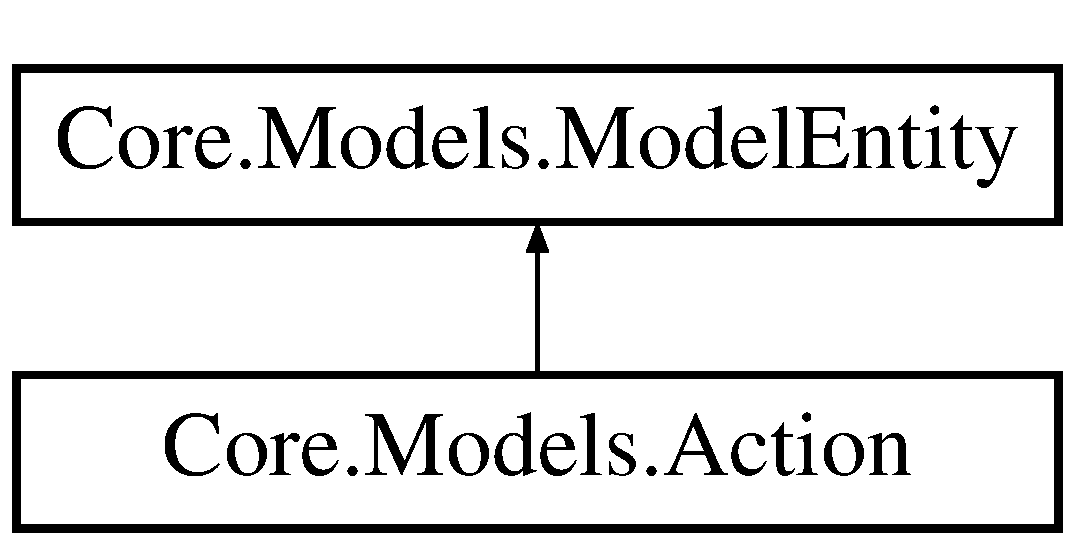
\includegraphics[height=1.296296cm]{classCore_1_1Models_1_1Action}
\end{center}
\end{figure}
\subsection*{Classes}
\begin{DoxyCompactItemize}
\item 
class \hyperlink{classCore_1_1Models_1_1Action_1_1ActionComparer}{Action\+Comparer}
\begin{DoxyCompactList}\small\item\em \hyperlink{classCore_1_1Models_1_1Action}{Action} comparer. \end{DoxyCompactList}\end{DoxyCompactItemize}
\subsection*{Public Types}
\begin{DoxyCompactItemize}
\item 
enum \hyperlink{classCore_1_1Models_1_1Action_a9e9cef4702eef3e7d99f5db15e8c4640}{Action\+Type} \{ \\*
{\bfseries Test\+Action}, 
{\bfseries Create\+Territory\+Building}, 
{\bfseries Create\+Building}, 
{\bfseries Create\+Unit}, 
\\*
{\bfseries Move\+Unit}
 \}\begin{DoxyCompactList}\small\item\em \hyperlink{classCore_1_1Models_1_1Action}{Action} type. \end{DoxyCompactList}
\end{DoxyCompactItemize}
\subsection*{Public Member Functions}
\begin{DoxyCompactItemize}
\item 
\hyperlink{classCore_1_1Models_1_1Action_ae4a71271ac1200f42b8dad22d565c939}{Action} (\hyperlink{classCore_1_1Models_1_1Account}{Account} account, \hyperlink{classCore_1_1Models_1_1Action_a9e9cef4702eef3e7d99f5db15e8c4640}{Action\+Type} type, Dictionary$<$ string, object $>$ parameters, Date\+Time?action\+Time=null)
\begin{DoxyCompactList}\small\item\em Initializes a new instance of the \hyperlink{classCore_1_1Models_1_1Action}{Core.\+Models.\+Action} class. \end{DoxyCompactList}\item 
override bool \hyperlink{classCore_1_1Models_1_1Action_a300fc2dc4c503f4ea9964846f9a434f0}{Equals} (object obj)
\begin{DoxyCompactList}\small\item\em tests if the given object is equal to this object \end{DoxyCompactList}\item 
override int \hyperlink{classCore_1_1Models_1_1Action_a29fa0c569250878b3f04d174cf5677ac}{Get\+Hash\+Code} ()
\begin{DoxyCompactList}\small\item\em standard hash function \end{DoxyCompactList}\end{DoxyCompactItemize}
\subsection*{Public Attributes}
\begin{DoxyCompactItemize}
\item 
int \hyperlink{classCore_1_1Models_1_1Action_a13671e1a48f3a462a366fe2768073816}{I\+D}
\begin{DoxyCompactList}\small\item\em Gets or Sets the I\+D \end{DoxyCompactList}\item 
Date\+Time \hyperlink{classCore_1_1Models_1_1Action_ab973fe9b8e3c6a60fa9d82cf53de57c3}{Action\+Time}
\begin{DoxyCompactList}\small\item\em The action time. \end{DoxyCompactList}\item 
\hyperlink{classCore_1_1Models_1_1Account}{Account} \hyperlink{classCore_1_1Models_1_1Action_a1924816082b3d1173ef309581a69ef95}{Account}
\begin{DoxyCompactList}\small\item\em The account. \end{DoxyCompactList}\end{DoxyCompactItemize}
\subsection*{Properties}
\begin{DoxyCompactItemize}
\item 
Dictionary$<$ string, object $>$ \hyperlink{classCore_1_1Models_1_1Action_a5b7b51347229bf4ca6ab02b419c476b8}{Parameters}\hspace{0.3cm}{\ttfamily  \mbox{[}get\mbox{]}}
\begin{DoxyCompactList}\small\item\em Gets the parameters. \end{DoxyCompactList}\item 
\hyperlink{classCore_1_1Models_1_1Action_a9e9cef4702eef3e7d99f5db15e8c4640}{Action\+Type} \hyperlink{classCore_1_1Models_1_1Action_abb5ac940b539ea5f61f866c219dcd858}{Type}\hspace{0.3cm}{\ttfamily  \mbox{[}get\mbox{]}}
\begin{DoxyCompactList}\small\item\em Gets the type. \end{DoxyCompactList}\item 
int \hyperlink{classCore_1_1Models_1_1Action_ae2defe30307109c1265b4cf16c001553}{Account\+I\+D}\hspace{0.3cm}{\ttfamily  \mbox{[}get, set\mbox{]}}
\begin{DoxyCompactList}\small\item\em Gets or sets the account I\+D. \end{DoxyCompactList}\end{DoxyCompactItemize}


\subsection{Detailed Description}
\hyperlink{classCore_1_1Models_1_1Action}{Action} model which should contains all needed data for the action control. 



\subsection{Member Enumeration Documentation}
\hypertarget{classCore_1_1Models_1_1Action_a9e9cef4702eef3e7d99f5db15e8c4640}{}\index{Core\+::\+Models\+::\+Action@{Core\+::\+Models\+::\+Action}!Action\+Type@{Action\+Type}}
\index{Action\+Type@{Action\+Type}!Core\+::\+Models\+::\+Action@{Core\+::\+Models\+::\+Action}}
\subsubsection[{Action\+Type}]{\setlength{\rightskip}{0pt plus 5cm}enum {\bf Core.\+Models.\+Action.\+Action\+Type}\hspace{0.3cm}{\ttfamily [strong]}}\label{classCore_1_1Models_1_1Action_a9e9cef4702eef3e7d99f5db15e8c4640}


\hyperlink{classCore_1_1Models_1_1Action}{Action} type. 



\subsection{Constructor \& Destructor Documentation}
\hypertarget{classCore_1_1Models_1_1Action_ae4a71271ac1200f42b8dad22d565c939}{}\index{Core\+::\+Models\+::\+Action@{Core\+::\+Models\+::\+Action}!Action@{Action}}
\index{Action@{Action}!Core\+::\+Models\+::\+Action@{Core\+::\+Models\+::\+Action}}
\subsubsection[{Action(\+Account account, Action\+Type type, Dictionary$<$ string, object $>$ parameters, Date\+Time?action\+Time=null)}]{\setlength{\rightskip}{0pt plus 5cm}Core.\+Models.\+Action.\+Action (
\begin{DoxyParamCaption}
\item[{{\bf Account}}]{account, }
\item[{{\bf Action\+Type}}]{type, }
\item[{Dictionary$<$ string, object $>$}]{parameters, }
\item[{Date\+Time?}]{action\+Time = {\ttfamily null}}
\end{DoxyParamCaption}
)}\label{classCore_1_1Models_1_1Action_ae4a71271ac1200f42b8dad22d565c939}


Initializes a new instance of the \hyperlink{classCore_1_1Models_1_1Action}{Core.\+Models.\+Action} class. 


\begin{DoxyParams}{Parameters}
{\em account} & \hyperlink{classCore_1_1Models_1_1Account}{Account} which wants to execute this action.\\
\hline
{\em type} & \hyperlink{classCore_1_1Models_1_1Action}{Action} Type.\\
\hline
{\em parameters} & Parameters which should contain all needed data by the action control.\\
\hline
{\em action\+Time} & Time when the action was executed.\\
\hline
\end{DoxyParams}


\subsection{Member Function Documentation}
\hypertarget{classCore_1_1Models_1_1Action_a300fc2dc4c503f4ea9964846f9a434f0}{}\index{Core\+::\+Models\+::\+Action@{Core\+::\+Models\+::\+Action}!Equals@{Equals}}
\index{Equals@{Equals}!Core\+::\+Models\+::\+Action@{Core\+::\+Models\+::\+Action}}
\subsubsection[{Equals(object obj)}]{\setlength{\rightskip}{0pt plus 5cm}override bool Core.\+Models.\+Action.\+Equals (
\begin{DoxyParamCaption}
\item[{object}]{obj}
\end{DoxyParamCaption}
)}\label{classCore_1_1Models_1_1Action_a300fc2dc4c503f4ea9964846f9a434f0}


tests if the given object is equal to this object 

\begin{DoxyReturn}{Returns}
true, if it is equal, otherwise false.
\end{DoxyReturn}

\begin{DoxyParams}{Parameters}
{\em obj} & The System.\+Object to compare with the current \hyperlink{classCore_1_1Models_1_1Action}{Core.\+Models.\+Action}.\\
\hline
\end{DoxyParams}
$<$filterpriority$>$2$<$/filterpriority$>$ \hypertarget{classCore_1_1Models_1_1Action_a29fa0c569250878b3f04d174cf5677ac}{}\index{Core\+::\+Models\+::\+Action@{Core\+::\+Models\+::\+Action}!Get\+Hash\+Code@{Get\+Hash\+Code}}
\index{Get\+Hash\+Code@{Get\+Hash\+Code}!Core\+::\+Models\+::\+Action@{Core\+::\+Models\+::\+Action}}
\subsubsection[{Get\+Hash\+Code()}]{\setlength{\rightskip}{0pt plus 5cm}override int Core.\+Models.\+Action.\+Get\+Hash\+Code (
\begin{DoxyParamCaption}
{}
\end{DoxyParamCaption}
)}\label{classCore_1_1Models_1_1Action_a29fa0c569250878b3f04d174cf5677ac}


standard hash function 

\begin{DoxyReturn}{Returns}
hash code.
\end{DoxyReturn}
$<$filterpriority$>$2$<$/filterpriority$>$ 

\subsection{Member Data Documentation}
\hypertarget{classCore_1_1Models_1_1Action_a1924816082b3d1173ef309581a69ef95}{}\index{Core\+::\+Models\+::\+Action@{Core\+::\+Models\+::\+Action}!Account@{Account}}
\index{Account@{Account}!Core\+::\+Models\+::\+Action@{Core\+::\+Models\+::\+Action}}
\subsubsection[{Account}]{\setlength{\rightskip}{0pt plus 5cm}{\bf Account} Core.\+Models.\+Action.\+Account}\label{classCore_1_1Models_1_1Action_a1924816082b3d1173ef309581a69ef95}


The account. 

\hypertarget{classCore_1_1Models_1_1Action_ab973fe9b8e3c6a60fa9d82cf53de57c3}{}\index{Core\+::\+Models\+::\+Action@{Core\+::\+Models\+::\+Action}!Action\+Time@{Action\+Time}}
\index{Action\+Time@{Action\+Time}!Core\+::\+Models\+::\+Action@{Core\+::\+Models\+::\+Action}}
\subsubsection[{Action\+Time}]{\setlength{\rightskip}{0pt plus 5cm}Date\+Time Core.\+Models.\+Action.\+Action\+Time}\label{classCore_1_1Models_1_1Action_ab973fe9b8e3c6a60fa9d82cf53de57c3}


The action time. 

\hypertarget{classCore_1_1Models_1_1Action_a13671e1a48f3a462a366fe2768073816}{}\index{Core\+::\+Models\+::\+Action@{Core\+::\+Models\+::\+Action}!I\+D@{I\+D}}
\index{I\+D@{I\+D}!Core\+::\+Models\+::\+Action@{Core\+::\+Models\+::\+Action}}
\subsubsection[{I\+D}]{\setlength{\rightskip}{0pt plus 5cm}int Core.\+Models.\+Action.\+I\+D}\label{classCore_1_1Models_1_1Action_a13671e1a48f3a462a366fe2768073816}


Gets or Sets the I\+D 



\subsection{Property Documentation}
\hypertarget{classCore_1_1Models_1_1Action_ae2defe30307109c1265b4cf16c001553}{}\index{Core\+::\+Models\+::\+Action@{Core\+::\+Models\+::\+Action}!Account\+I\+D@{Account\+I\+D}}
\index{Account\+I\+D@{Account\+I\+D}!Core\+::\+Models\+::\+Action@{Core\+::\+Models\+::\+Action}}
\subsubsection[{Account\+I\+D}]{\setlength{\rightskip}{0pt plus 5cm}int Core.\+Models.\+Action.\+Account\+I\+D\hspace{0.3cm}{\ttfamily [get]}, {\ttfamily [set]}}\label{classCore_1_1Models_1_1Action_ae2defe30307109c1265b4cf16c001553}


Gets or sets the account I\+D. 

The account I\+D.\hypertarget{classCore_1_1Models_1_1Action_a5b7b51347229bf4ca6ab02b419c476b8}{}\index{Core\+::\+Models\+::\+Action@{Core\+::\+Models\+::\+Action}!Parameters@{Parameters}}
\index{Parameters@{Parameters}!Core\+::\+Models\+::\+Action@{Core\+::\+Models\+::\+Action}}
\subsubsection[{Parameters}]{\setlength{\rightskip}{0pt plus 5cm}Dictionary$<$string, object$>$ Core.\+Models.\+Action.\+Parameters\hspace{0.3cm}{\ttfamily [get]}}\label{classCore_1_1Models_1_1Action_a5b7b51347229bf4ca6ab02b419c476b8}


Gets the parameters. 

The parameters.\hypertarget{classCore_1_1Models_1_1Action_abb5ac940b539ea5f61f866c219dcd858}{}\index{Core\+::\+Models\+::\+Action@{Core\+::\+Models\+::\+Action}!Type@{Type}}
\index{Type@{Type}!Core\+::\+Models\+::\+Action@{Core\+::\+Models\+::\+Action}}
\subsubsection[{Type}]{\setlength{\rightskip}{0pt plus 5cm}{\bf Action\+Type} Core.\+Models.\+Action.\+Type\hspace{0.3cm}{\ttfamily [get]}}\label{classCore_1_1Models_1_1Action_abb5ac940b539ea5f61f866c219dcd858}


Gets the type. 

The type.

The documentation for this class was generated from the following file\+:\begin{DoxyCompactItemize}
\item 
base/\+Models/Action.\+cs\end{DoxyCompactItemize}

\hypertarget{classCore_1_1Models_1_1Action_1_1ActionComparer}{\section{Core.\-Models.\-Action.\-Action\-Comparer Class Reference}
\label{classCore_1_1Models_1_1Action_1_1ActionComparer}\index{Core.\-Models.\-Action.\-Action\-Comparer@{Core.\-Models.\-Action.\-Action\-Comparer}}
}
Inheritance diagram for Core.\-Models.\-Action.\-Action\-Comparer\-:\begin{figure}[H]
\begin{center}
\leavevmode
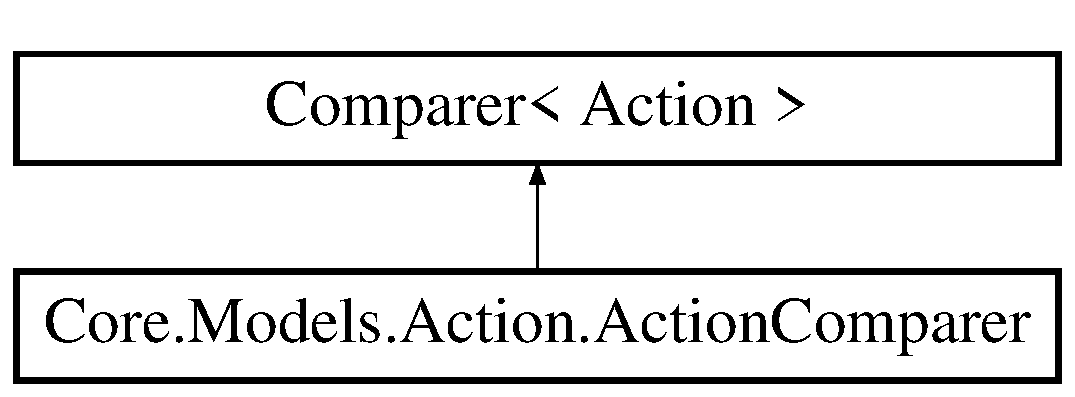
\includegraphics[height=2.000000cm]{classCore_1_1Models_1_1Action_1_1ActionComparer}
\end{center}
\end{figure}
\subsection*{Public Member Functions}
\begin{DoxyCompactItemize}
\item 
\hypertarget{classCore_1_1Models_1_1Action_1_1ActionComparer_a876fafb59816fb7f9b7c0c35a9312c7a}{override int {\bfseries Compare} (\hyperlink{classCore_1_1Models_1_1Action}{Action} first, \hyperlink{classCore_1_1Models_1_1Action}{Action} second)}\label{classCore_1_1Models_1_1Action_1_1ActionComparer_a876fafb59816fb7f9b7c0c35a9312c7a}

\end{DoxyCompactItemize}


The documentation for this class was generated from the following file\-:\begin{DoxyCompactItemize}
\item 
base/\-Models/Action.\-cs\end{DoxyCompactItemize}

\hypertarget{classClient_1_1Common_1_1Helper_1_1ActionHelper}{}\section{Client.\+Common.\+Helper.\+Action\+Helper Class Reference}
\label{classClient_1_1Common_1_1Helper_1_1ActionHelper}\index{Client.\+Common.\+Helper.\+Action\+Helper@{Client.\+Common.\+Helper.\+Action\+Helper}}


The Action helper create actions.  


\subsection*{Static Public Member Functions}
\begin{DoxyCompactItemize}
\item 
static \hyperlink{classCore_1_1Models_1_1Action}{Core.\+Models.\+Action} \hyperlink{classClient_1_1Common_1_1Helper_1_1ActionHelper_a57696e59e0d3a58e65b720e79aeffb26}{Move\+Unit} (\hyperlink{classCore_1_1Models_1_1PositionI}{Position\+I} start, \hyperlink{classCore_1_1Models_1_1PositionI}{Position\+I} end)
\begin{DoxyCompactList}\small\item\em Creates the action to move a unit. \end{DoxyCompactList}\item 
static \hyperlink{classCore_1_1Models_1_1Action}{Core.\+Models.\+Action} \hyperlink{classClient_1_1Common_1_1Helper_1_1ActionHelper_a0e7689f40d850a8670d803028e249711}{Create\+Entity} (\hyperlink{classCore_1_1Models_1_1PositionI}{Position\+I} position\+I, \hyperlink{classCore_1_1Models_1_1Definitions_1_1Definition}{Core.\+Models.\+Definitions.\+Definition} definition, \hyperlink{classCore_1_1Models_1_1Account}{Account} account)
\begin{DoxyCompactList}\small\item\em Creates the action which creates the unit \end{DoxyCompactList}\end{DoxyCompactItemize}


\subsection{Detailed Description}
The Action helper create actions. 



\subsection{Member Function Documentation}
\hypertarget{classClient_1_1Common_1_1Helper_1_1ActionHelper_a0e7689f40d850a8670d803028e249711}{}\index{Client\+::\+Common\+::\+Helper\+::\+Action\+Helper@{Client\+::\+Common\+::\+Helper\+::\+Action\+Helper}!Create\+Entity@{Create\+Entity}}
\index{Create\+Entity@{Create\+Entity}!Client\+::\+Common\+::\+Helper\+::\+Action\+Helper@{Client\+::\+Common\+::\+Helper\+::\+Action\+Helper}}
\subsubsection[{Create\+Entity(\+Position\+I position\+I, Core.\+Models.\+Definitions.\+Definition definition, Account account)}]{\setlength{\rightskip}{0pt plus 5cm}static {\bf Core.\+Models.\+Action} Client.\+Common.\+Helper.\+Action\+Helper.\+Create\+Entity (
\begin{DoxyParamCaption}
\item[{{\bf Position\+I}}]{position\+I, }
\item[{{\bf Core.\+Models.\+Definitions.\+Definition}}]{definition, }
\item[{{\bf Account}}]{account}
\end{DoxyParamCaption}
)\hspace{0.3cm}{\ttfamily [static]}}\label{classClient_1_1Common_1_1Helper_1_1ActionHelper_a0e7689f40d850a8670d803028e249711}


Creates the action which creates the unit 

\begin{DoxyReturn}{Returns}
The entity create action.
\end{DoxyReturn}

\begin{DoxyParams}{Parameters}
{\em position\+I} & Position where the entity should be created.\\
\hline
{\em definition} & Definition which entity should be created.\\
\hline
{\em account} & Which account creates the action.\\
\hline
\end{DoxyParams}
\hypertarget{classClient_1_1Common_1_1Helper_1_1ActionHelper_a57696e59e0d3a58e65b720e79aeffb26}{}\index{Client\+::\+Common\+::\+Helper\+::\+Action\+Helper@{Client\+::\+Common\+::\+Helper\+::\+Action\+Helper}!Move\+Unit@{Move\+Unit}}
\index{Move\+Unit@{Move\+Unit}!Client\+::\+Common\+::\+Helper\+::\+Action\+Helper@{Client\+::\+Common\+::\+Helper\+::\+Action\+Helper}}
\subsubsection[{Move\+Unit(\+Position\+I start, Position\+I end)}]{\setlength{\rightskip}{0pt plus 5cm}static {\bf Core.\+Models.\+Action} Client.\+Common.\+Helper.\+Action\+Helper.\+Move\+Unit (
\begin{DoxyParamCaption}
\item[{{\bf Position\+I}}]{start, }
\item[{{\bf Position\+I}}]{end}
\end{DoxyParamCaption}
)\hspace{0.3cm}{\ttfamily [static]}}\label{classClient_1_1Common_1_1Helper_1_1ActionHelper_a57696e59e0d3a58e65b720e79aeffb26}


Creates the action to move a unit. 

\begin{DoxyReturn}{Returns}
The move unit action.
\end{DoxyReturn}

\begin{DoxyParams}{Parameters}
{\em start} & Start position of move.\\
\hline
{\em end} & End position of move.\\
\hline
\end{DoxyParams}


The documentation for this class was generated from the following file\+:\begin{DoxyCompactItemize}
\item 
client/client/client.\+Common/\+Helper/Action\+Helper.\+cs\end{DoxyCompactItemize}

\hypertarget{classServer_1_1Controllers_1_1APIController}{}\section{Server.\+Controllers.\+A\+P\+I\+Controller Class Reference}
\label{classServer_1_1Controllers_1_1APIController}\index{Server.\+Controllers.\+A\+P\+I\+Controller@{Server.\+Controllers.\+A\+P\+I\+Controller}}


A\+P\+I Controller provides functionality to access the game. Every access from outside should use A\+P\+I Controller. As example H\+T\+T\+P\+Controller uses only A\+P\+I Controller. If we later switch to another protocol (or directly sockets) we just need to build another H\+T\+T\+P Controller-\/like which uses the A\+P\+I Controller functionality.  


\subsection*{Classes}
\begin{DoxyCompactItemize}
\item 
class \hyperlink{classServer_1_1Controllers_1_1APIController_1_1RegionData}{Region\+Data}
\begin{DoxyCompactList}\small\item\em Region data. \end{DoxyCompactList}\end{DoxyCompactItemize}
\subsection*{Public Member Functions}
\begin{DoxyCompactItemize}
\item 
\hyperlink{classCore_1_1Models_1_1Account}{Core.\+Models.\+Account} \hyperlink{classServer_1_1Controllers_1_1APIController_a00ed79b2c42e5c4f39319c38fc492b32}{Login} (string username, string password)
\begin{DoxyCompactList}\small\item\em Login with a username und password, returns Account if everything worked, otherwise {\bfseries null} \end{DoxyCompactList}\item 
void \hyperlink{classServer_1_1Controllers_1_1APIController_abca86085e8c85b2f94b0a95e47a89add}{Do\+Action} (\hyperlink{classCore_1_1Models_1_1Account}{Core.\+Models.\+Account} account, \hyperlink{classCore_1_1Models_1_1Action}{Core.\+Models.\+Action}\mbox{[}$\,$\mbox{]} actions)
\begin{DoxyCompactList}\small\item\em Send Actions the server so they will be executed. (but first, the actions have to wait in a queue) \end{DoxyCompactList}\item 
\hyperlink{classServer_1_1Controllers_1_1APIController_1_1RegionData}{Region\+Data} \hyperlink{classServer_1_1Controllers_1_1APIController_a109e88f8d8e2006aa6408ae775779864}{Load\+Regions} (\hyperlink{classCore_1_1Models_1_1Account}{Core.\+Models.\+Account} account, \hyperlink{classCore_1_1Models_1_1RegionPosition}{Core.\+Models.\+Region\+Position}\mbox{[}$\,$\mbox{]} region\+Positions)
\begin{DoxyCompactList}\small\item\em Loads the regions. \end{DoxyCompactList}\item 
void \hyperlink{classServer_1_1Controllers_1_1APIController_ab0452ab5e12d38f778cc5db9b41bb3a0}{Worker} (object state)
\begin{DoxyCompactList}\small\item\em Worker (normally an own thread) which runs until the application finishes. \end{DoxyCompactList}\end{DoxyCompactItemize}
\subsection*{Properties}
\begin{DoxyCompactItemize}
\item 
static \hyperlink{classServer_1_1Controllers_1_1APIController}{A\+P\+I\+Controller} \hyperlink{classServer_1_1Controllers_1_1APIController_aba201431eb3c55a67e96f3afb2751fc9}{Instance}\hspace{0.3cm}{\ttfamily  \mbox{[}get\mbox{]}}
\begin{DoxyCompactList}\small\item\em Gets the singleton instance. \end{DoxyCompactList}\end{DoxyCompactItemize}


\subsection{Detailed Description}
A\+P\+I Controller provides functionality to access the game. Every access from outside should use A\+P\+I Controller. As example H\+T\+T\+P\+Controller uses only A\+P\+I Controller. If we later switch to another protocol (or directly sockets) we just need to build another H\+T\+T\+P Controller-\/like which uses the A\+P\+I Controller functionality. 



\subsection{Member Function Documentation}
\hypertarget{classServer_1_1Controllers_1_1APIController_abca86085e8c85b2f94b0a95e47a89add}{}\index{Server\+::\+Controllers\+::\+A\+P\+I\+Controller@{Server\+::\+Controllers\+::\+A\+P\+I\+Controller}!Do\+Action@{Do\+Action}}
\index{Do\+Action@{Do\+Action}!Server\+::\+Controllers\+::\+A\+P\+I\+Controller@{Server\+::\+Controllers\+::\+A\+P\+I\+Controller}}
\subsubsection[{Do\+Action(\+Core.\+Models.\+Account account, Core.\+Models.\+Action[] actions)}]{\setlength{\rightskip}{0pt plus 5cm}void Server.\+Controllers.\+A\+P\+I\+Controller.\+Do\+Action (
\begin{DoxyParamCaption}
\item[{{\bf Core.\+Models.\+Account}}]{account, }
\item[{{\bf Core.\+Models.\+Action}\mbox{[}$\,$\mbox{]}}]{actions}
\end{DoxyParamCaption}
)}\label{classServer_1_1Controllers_1_1APIController_abca86085e8c85b2f94b0a95e47a89add}


Send Actions the server so they will be executed. (but first, the actions have to wait in a queue) 


\begin{DoxyParams}{Parameters}
{\em account} & Account who wants the actions executed.\\
\hline
{\em actions} & Array of Actions which should be executed.\\
\hline
\end{DoxyParams}
\hypertarget{classServer_1_1Controllers_1_1APIController_a109e88f8d8e2006aa6408ae775779864}{}\index{Server\+::\+Controllers\+::\+A\+P\+I\+Controller@{Server\+::\+Controllers\+::\+A\+P\+I\+Controller}!Load\+Regions@{Load\+Regions}}
\index{Load\+Regions@{Load\+Regions}!Server\+::\+Controllers\+::\+A\+P\+I\+Controller@{Server\+::\+Controllers\+::\+A\+P\+I\+Controller}}
\subsubsection[{Load\+Regions(\+Core.\+Models.\+Account account, Core.\+Models.\+Region\+Position[] region\+Positions)}]{\setlength{\rightskip}{0pt plus 5cm}{\bf Region\+Data} Server.\+Controllers.\+A\+P\+I\+Controller.\+Load\+Regions (
\begin{DoxyParamCaption}
\item[{{\bf Core.\+Models.\+Account}}]{account, }
\item[{{\bf Core.\+Models.\+Region\+Position}\mbox{[}$\,$\mbox{]}}]{region\+Positions}
\end{DoxyParamCaption}
)}\label{classServer_1_1Controllers_1_1APIController_a109e88f8d8e2006aa6408ae775779864}


Loads the regions. 

\begin{DoxyReturn}{Returns}
The regions.
\end{DoxyReturn}

\begin{DoxyParams}{Parameters}
{\em account} & Account who wants the load the regions.\\
\hline
{\em region\+Positions} & Positions of the regions.\\
\hline
\end{DoxyParams}
\hypertarget{classServer_1_1Controllers_1_1APIController_a00ed79b2c42e5c4f39319c38fc492b32}{}\index{Server\+::\+Controllers\+::\+A\+P\+I\+Controller@{Server\+::\+Controllers\+::\+A\+P\+I\+Controller}!Login@{Login}}
\index{Login@{Login}!Server\+::\+Controllers\+::\+A\+P\+I\+Controller@{Server\+::\+Controllers\+::\+A\+P\+I\+Controller}}
\subsubsection[{Login(string username, string password)}]{\setlength{\rightskip}{0pt plus 5cm}{\bf Core.\+Models.\+Account} Server.\+Controllers.\+A\+P\+I\+Controller.\+Login (
\begin{DoxyParamCaption}
\item[{string}]{username, }
\item[{string}]{password}
\end{DoxyParamCaption}
)}\label{classServer_1_1Controllers_1_1APIController_a00ed79b2c42e5c4f39319c38fc492b32}


Login with a username und password, returns Account if everything worked, otherwise {\bfseries null} 


\begin{DoxyParams}{Parameters}
{\em username} & Account Username.\\
\hline
{\em password} & Account Password.\\
\hline
\end{DoxyParams}
\begin{DoxyReturn}{Returns}
Account if login worked. Otherwise {\bfseries null}
\end{DoxyReturn}
\hypertarget{classServer_1_1Controllers_1_1APIController_ab0452ab5e12d38f778cc5db9b41bb3a0}{}\index{Server\+::\+Controllers\+::\+A\+P\+I\+Controller@{Server\+::\+Controllers\+::\+A\+P\+I\+Controller}!Worker@{Worker}}
\index{Worker@{Worker}!Server\+::\+Controllers\+::\+A\+P\+I\+Controller@{Server\+::\+Controllers\+::\+A\+P\+I\+Controller}}
\subsubsection[{Worker(object state)}]{\setlength{\rightskip}{0pt plus 5cm}void Server.\+Controllers.\+A\+P\+I\+Controller.\+Worker (
\begin{DoxyParamCaption}
\item[{object}]{state}
\end{DoxyParamCaption}
)}\label{classServer_1_1Controllers_1_1APIController_ab0452ab5e12d38f778cc5db9b41bb3a0}


Worker (normally an own thread) which runs until the application finishes. 


\begin{DoxyParams}{Parameters}
{\em state} & Threading Number (for queue association)\\
\hline
\end{DoxyParams}


\subsection{Property Documentation}
\hypertarget{classServer_1_1Controllers_1_1APIController_aba201431eb3c55a67e96f3afb2751fc9}{}\index{Server\+::\+Controllers\+::\+A\+P\+I\+Controller@{Server\+::\+Controllers\+::\+A\+P\+I\+Controller}!Instance@{Instance}}
\index{Instance@{Instance}!Server\+::\+Controllers\+::\+A\+P\+I\+Controller@{Server\+::\+Controllers\+::\+A\+P\+I\+Controller}}
\subsubsection[{Instance}]{\setlength{\rightskip}{0pt plus 5cm}{\bf A\+P\+I\+Controller} Server.\+Controllers.\+A\+P\+I\+Controller.\+Instance\hspace{0.3cm}{\ttfamily [static]}, {\ttfamily [get]}}\label{classServer_1_1Controllers_1_1APIController_aba201431eb3c55a67e96f3afb2751fc9}


Gets the singleton instance. 

The instance.

The documentation for this class was generated from the following file\+:\begin{DoxyCompactItemize}
\item 
tcpserver/\+Controllers/A\+P\+I\+Controller.\+cs\end{DoxyCompactItemize}

\hypertarget{classClient_1_1iOS_1_1AppDelegate}{\section{Client.\-i\-O\-S.\-App\-Delegate Class Reference}
\label{classClient_1_1iOS_1_1AppDelegate}\index{Client.\-i\-O\-S.\-App\-Delegate@{Client.\-i\-O\-S.\-App\-Delegate}}
}
Inheritance diagram for Client.\-i\-O\-S.\-App\-Delegate\-:\begin{figure}[H]
\begin{center}
\leavevmode
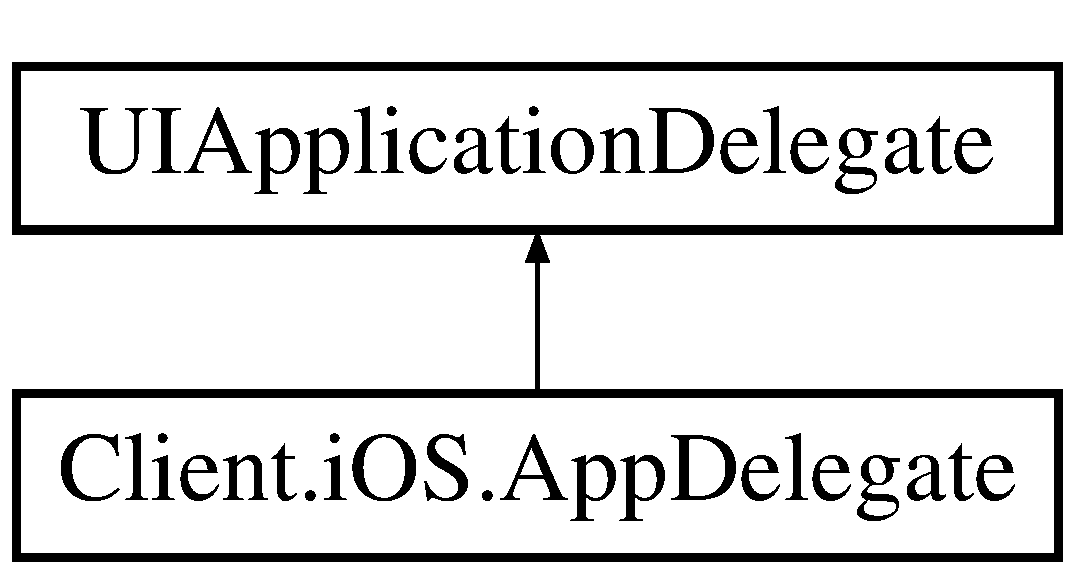
\includegraphics[height=2.000000cm]{classClient_1_1iOS_1_1AppDelegate}
\end{center}
\end{figure}
\subsection*{Public Member Functions}
\begin{DoxyCompactItemize}
\item 
\hypertarget{classClient_1_1iOS_1_1AppDelegate_aa0ee3c7acee2f19211c95e6eb7fe00af}{override void {\bfseries Finished\-Launching} (U\-I\-Application app)}\label{classClient_1_1iOS_1_1AppDelegate_aa0ee3c7acee2f19211c95e6eb7fe00af}

\end{DoxyCompactItemize}


The documentation for this class was generated from the following file\-:\begin{DoxyCompactItemize}
\item 
client/client/client.\-i\-O\-S/App\-Delegate.\-cs\end{DoxyCompactItemize}

\hypertarget{classserver_1_1Models_1_1DAL_1_1ASDInitializer}{\section{server.\-Models.\-D\-A\-L.\-A\-S\-D\-Initializer Class Reference}
\label{classserver_1_1Models_1_1DAL_1_1ASDInitializer}\index{server.\-Models.\-D\-A\-L.\-A\-S\-D\-Initializer@{server.\-Models.\-D\-A\-L.\-A\-S\-D\-Initializer}}
}
Inheritance diagram for server.\-Models.\-D\-A\-L.\-A\-S\-D\-Initializer\-:\begin{figure}[H]
\begin{center}
\leavevmode
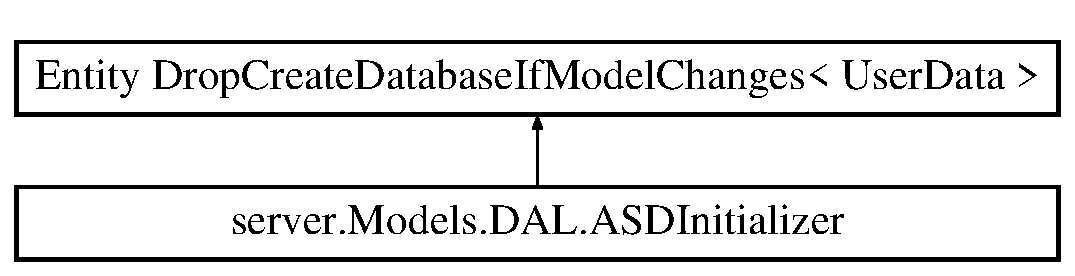
\includegraphics[height=2.000000cm]{classserver_1_1Models_1_1DAL_1_1ASDInitializer}
\end{center}
\end{figure}
\subsection*{Protected Member Functions}
\begin{DoxyCompactItemize}
\item 
\hypertarget{classserver_1_1Models_1_1DAL_1_1ASDInitializer_afd9f60e98d02493a855949dfc8cc7cee}{override void {\bfseries Seed} (\hyperlink{classserver_1_1Models_1_1DAL_1_1UserData}{User\-Data} context)}\label{classserver_1_1Models_1_1DAL_1_1ASDInitializer_afd9f60e98d02493a855949dfc8cc7cee}

\end{DoxyCompactItemize}


The documentation for this class was generated from the following file\-:\begin{DoxyCompactItemize}
\item 
server/\-Models/\-D\-A\-L/A\-S\-D\-Initializer.\-cs\end{DoxyCompactItemize}

\hypertarget{classSQLite_1_1AsyncTableQuery_3_01T_01_4}{\section{S\-Q\-Lite.\-Async\-Table\-Query$<$ T $>$ Class Template Reference}
\label{classSQLite_1_1AsyncTableQuery_3_01T_01_4}\index{S\-Q\-Lite.\-Async\-Table\-Query$<$ T $>$@{S\-Q\-Lite.\-Async\-Table\-Query$<$ T $>$}}
}
\subsection*{Public Member Functions}
\begin{DoxyCompactItemize}
\item 
\hypertarget{classSQLite_1_1AsyncTableQuery_3_01T_01_4_a0255986ac768d5fca5b4e2c9840da35d}{{\bfseries Async\-Table\-Query} (Table\-Query$<$ T $>$ inner\-Query)}\label{classSQLite_1_1AsyncTableQuery_3_01T_01_4_a0255986ac768d5fca5b4e2c9840da35d}

\item 
\hypertarget{classSQLite_1_1AsyncTableQuery_3_01T_01_4_afe04f8363082a033b984230c7a245dea}{Async\-Table\-Query$<$ T $>$ {\bfseries Where} (Expression$<$ Func$<$ T, bool $>$$>$ pred\-Expr)}\label{classSQLite_1_1AsyncTableQuery_3_01T_01_4_afe04f8363082a033b984230c7a245dea}

\item 
\hypertarget{classSQLite_1_1AsyncTableQuery_3_01T_01_4_ab1b8210413273abe6bc9383bc4f7ea9c}{Async\-Table\-Query$<$ T $>$ {\bfseries Skip} (int n)}\label{classSQLite_1_1AsyncTableQuery_3_01T_01_4_ab1b8210413273abe6bc9383bc4f7ea9c}

\item 
\hypertarget{classSQLite_1_1AsyncTableQuery_3_01T_01_4_a6c47c652b3b8123e2d4961263c289af9}{Async\-Table\-Query$<$ T $>$ {\bfseries Take} (int n)}\label{classSQLite_1_1AsyncTableQuery_3_01T_01_4_a6c47c652b3b8123e2d4961263c289af9}

\item 
\hypertarget{classSQLite_1_1AsyncTableQuery_3_01T_01_4_a41540b08c3c49c123b57de8a0a5e3aea}{Async\-Table\-Query$<$ T $>$ {\bfseries Order\-By$<$ U $>$} (Expression$<$ Func$<$ T, U $>$$>$ order\-Expr)}\label{classSQLite_1_1AsyncTableQuery_3_01T_01_4_a41540b08c3c49c123b57de8a0a5e3aea}

\item 
\hypertarget{classSQLite_1_1AsyncTableQuery_3_01T_01_4_a4a45b5c81ccf4459f17d66fba6a18c3f}{Async\-Table\-Query$<$ T $>$ {\bfseries Order\-By\-Descending$<$ U $>$} (Expression$<$ Func$<$ T, U $>$$>$ order\-Expr)}\label{classSQLite_1_1AsyncTableQuery_3_01T_01_4_a4a45b5c81ccf4459f17d66fba6a18c3f}

\item 
\hypertarget{classSQLite_1_1AsyncTableQuery_3_01T_01_4_a7343ff525af21bdc055935f46a39ae72}{Task$<$ List$<$ T $>$ $>$ {\bfseries To\-List\-Async} ()}\label{classSQLite_1_1AsyncTableQuery_3_01T_01_4_a7343ff525af21bdc055935f46a39ae72}

\item 
\hypertarget{classSQLite_1_1AsyncTableQuery_3_01T_01_4_a70df4365834cfe29d0adb1c1841266b0}{Task$<$ int $>$ {\bfseries Count\-Async} ()}\label{classSQLite_1_1AsyncTableQuery_3_01T_01_4_a70df4365834cfe29d0adb1c1841266b0}

\item 
\hypertarget{classSQLite_1_1AsyncTableQuery_3_01T_01_4_ade7303c76081c4b9cd80b4d25806ca30}{Task$<$ T $>$ {\bfseries Element\-At\-Async} (int index)}\label{classSQLite_1_1AsyncTableQuery_3_01T_01_4_ade7303c76081c4b9cd80b4d25806ca30}

\item 
\hypertarget{classSQLite_1_1AsyncTableQuery_3_01T_01_4_a2e3bae8cc7dc0b16abd95d4516d61971}{Task$<$ T $>$ {\bfseries First\-Async} ()}\label{classSQLite_1_1AsyncTableQuery_3_01T_01_4_a2e3bae8cc7dc0b16abd95d4516d61971}

\item 
\hypertarget{classSQLite_1_1AsyncTableQuery_3_01T_01_4_aac82a5fa254a7f1c6a1a08f534989604}{Task$<$ T $>$ {\bfseries First\-Or\-Default\-Async} ()}\label{classSQLite_1_1AsyncTableQuery_3_01T_01_4_aac82a5fa254a7f1c6a1a08f534989604}

\item 
\hypertarget{classSQLite_1_1AsyncTableQuery_3_01T_01_4_a0255986ac768d5fca5b4e2c9840da35d}{{\bfseries Async\-Table\-Query} (Table\-Query$<$ T $>$ inner\-Query)}\label{classSQLite_1_1AsyncTableQuery_3_01T_01_4_a0255986ac768d5fca5b4e2c9840da35d}

\item 
\hypertarget{classSQLite_1_1AsyncTableQuery_3_01T_01_4_afe04f8363082a033b984230c7a245dea}{Async\-Table\-Query$<$ T $>$ {\bfseries Where} (Expression$<$ Func$<$ T, bool $>$$>$ pred\-Expr)}\label{classSQLite_1_1AsyncTableQuery_3_01T_01_4_afe04f8363082a033b984230c7a245dea}

\item 
\hypertarget{classSQLite_1_1AsyncTableQuery_3_01T_01_4_ab1b8210413273abe6bc9383bc4f7ea9c}{Async\-Table\-Query$<$ T $>$ {\bfseries Skip} (int n)}\label{classSQLite_1_1AsyncTableQuery_3_01T_01_4_ab1b8210413273abe6bc9383bc4f7ea9c}

\item 
\hypertarget{classSQLite_1_1AsyncTableQuery_3_01T_01_4_a6c47c652b3b8123e2d4961263c289af9}{Async\-Table\-Query$<$ T $>$ {\bfseries Take} (int n)}\label{classSQLite_1_1AsyncTableQuery_3_01T_01_4_a6c47c652b3b8123e2d4961263c289af9}

\item 
\hypertarget{classSQLite_1_1AsyncTableQuery_3_01T_01_4_a41540b08c3c49c123b57de8a0a5e3aea}{Async\-Table\-Query$<$ T $>$ {\bfseries Order\-By$<$ U $>$} (Expression$<$ Func$<$ T, U $>$$>$ order\-Expr)}\label{classSQLite_1_1AsyncTableQuery_3_01T_01_4_a41540b08c3c49c123b57de8a0a5e3aea}

\item 
\hypertarget{classSQLite_1_1AsyncTableQuery_3_01T_01_4_a4a45b5c81ccf4459f17d66fba6a18c3f}{Async\-Table\-Query$<$ T $>$ {\bfseries Order\-By\-Descending$<$ U $>$} (Expression$<$ Func$<$ T, U $>$$>$ order\-Expr)}\label{classSQLite_1_1AsyncTableQuery_3_01T_01_4_a4a45b5c81ccf4459f17d66fba6a18c3f}

\item 
\hypertarget{classSQLite_1_1AsyncTableQuery_3_01T_01_4_a7343ff525af21bdc055935f46a39ae72}{Task$<$ List$<$ T $>$ $>$ {\bfseries To\-List\-Async} ()}\label{classSQLite_1_1AsyncTableQuery_3_01T_01_4_a7343ff525af21bdc055935f46a39ae72}

\item 
\hypertarget{classSQLite_1_1AsyncTableQuery_3_01T_01_4_a70df4365834cfe29d0adb1c1841266b0}{Task$<$ int $>$ {\bfseries Count\-Async} ()}\label{classSQLite_1_1AsyncTableQuery_3_01T_01_4_a70df4365834cfe29d0adb1c1841266b0}

\item 
\hypertarget{classSQLite_1_1AsyncTableQuery_3_01T_01_4_ade7303c76081c4b9cd80b4d25806ca30}{Task$<$ T $>$ {\bfseries Element\-At\-Async} (int index)}\label{classSQLite_1_1AsyncTableQuery_3_01T_01_4_ade7303c76081c4b9cd80b4d25806ca30}

\item 
\hypertarget{classSQLite_1_1AsyncTableQuery_3_01T_01_4_a2e3bae8cc7dc0b16abd95d4516d61971}{Task$<$ T $>$ {\bfseries First\-Async} ()}\label{classSQLite_1_1AsyncTableQuery_3_01T_01_4_a2e3bae8cc7dc0b16abd95d4516d61971}

\item 
\hypertarget{classSQLite_1_1AsyncTableQuery_3_01T_01_4_aac82a5fa254a7f1c6a1a08f534989604}{Task$<$ T $>$ {\bfseries First\-Or\-Default\-Async} ()}\label{classSQLite_1_1AsyncTableQuery_3_01T_01_4_aac82a5fa254a7f1c6a1a08f534989604}

\end{DoxyCompactItemize}


The documentation for this class was generated from the following file\-:\begin{DoxyCompactItemize}
\item 
packages/sqlite-\/net.\-1.\-0.\-8/content/S\-Q\-Lite\-Async.\-cs\end{DoxyCompactItemize}

\hypertarget{classClient_1_1Droid_1_1Resource_1_1Attribute}{}\section{Client.\+Droid.\+Resource.\+Attribute Class Reference}
\label{classClient_1_1Droid_1_1Resource_1_1Attribute}\index{Client.\+Droid.\+Resource.\+Attribute@{Client.\+Droid.\+Resource.\+Attribute}}
\subsection*{Public Attributes}
\begin{DoxyCompactItemize}
\item 
\hypertarget{classClient_1_1Droid_1_1Resource_1_1Attribute_a19ce72f78e25ccd3d7a913a2b274a69d}{}const int {\bfseries action\+Bar\+Divider} = 2130772143\label{classClient_1_1Droid_1_1Resource_1_1Attribute_a19ce72f78e25ccd3d7a913a2b274a69d}

\item 
\hypertarget{classClient_1_1Droid_1_1Resource_1_1Attribute_a8d3654407d69378cf3c5ed47e9508e61}{}const int {\bfseries action\+Bar\+Item\+Background} = 2130772144\label{classClient_1_1Droid_1_1Resource_1_1Attribute_a8d3654407d69378cf3c5ed47e9508e61}

\item 
\hypertarget{classClient_1_1Droid_1_1Resource_1_1Attribute_ab302b742baecf13b218c74252572a394}{}const int {\bfseries action\+Bar\+Popup\+Theme} = 2130772137\label{classClient_1_1Droid_1_1Resource_1_1Attribute_ab302b742baecf13b218c74252572a394}

\item 
\hypertarget{classClient_1_1Droid_1_1Resource_1_1Attribute_ae37184d3a328eb327d20d4634e23f54c}{}const int {\bfseries action\+Bar\+Size} = 2130772142\label{classClient_1_1Droid_1_1Resource_1_1Attribute_ae37184d3a328eb327d20d4634e23f54c}

\item 
\hypertarget{classClient_1_1Droid_1_1Resource_1_1Attribute_a4a3e37bbfa2e4f85c1fcfaf7712c0b8b}{}const int {\bfseries action\+Bar\+Split\+Style} = 2130772139\label{classClient_1_1Droid_1_1Resource_1_1Attribute_a4a3e37bbfa2e4f85c1fcfaf7712c0b8b}

\item 
\hypertarget{classClient_1_1Droid_1_1Resource_1_1Attribute_a600def35c8e7cd908fe05007161ae5c9}{}const int {\bfseries action\+Bar\+Style} = 2130772138\label{classClient_1_1Droid_1_1Resource_1_1Attribute_a600def35c8e7cd908fe05007161ae5c9}

\item 
\hypertarget{classClient_1_1Droid_1_1Resource_1_1Attribute_ae264e85ef6b00011af66b05df9f9cd33}{}const int {\bfseries action\+Bar\+Tab\+Bar\+Style} = 2130772133\label{classClient_1_1Droid_1_1Resource_1_1Attribute_ae264e85ef6b00011af66b05df9f9cd33}

\item 
\hypertarget{classClient_1_1Droid_1_1Resource_1_1Attribute_a8d9ca739363b08ac96e4c0e128b0af7e}{}const int {\bfseries action\+Bar\+Tab\+Style} = 2130772132\label{classClient_1_1Droid_1_1Resource_1_1Attribute_a8d9ca739363b08ac96e4c0e128b0af7e}

\item 
\hypertarget{classClient_1_1Droid_1_1Resource_1_1Attribute_ab3ed7d9dd62ab790cbff4f427d490434}{}const int {\bfseries action\+Bar\+Tab\+Text\+Style} = 2130772134\label{classClient_1_1Droid_1_1Resource_1_1Attribute_ab3ed7d9dd62ab790cbff4f427d490434}

\item 
\hypertarget{classClient_1_1Droid_1_1Resource_1_1Attribute_a19c18047d00ccf3d133c861c00c6d85d}{}const int {\bfseries action\+Bar\+Theme} = 2130772140\label{classClient_1_1Droid_1_1Resource_1_1Attribute_a19c18047d00ccf3d133c861c00c6d85d}

\item 
\hypertarget{classClient_1_1Droid_1_1Resource_1_1Attribute_aec9d7746de285c78bdba65a0b07938ba}{}const int {\bfseries action\+Bar\+Widget\+Theme} = 2130772141\label{classClient_1_1Droid_1_1Resource_1_1Attribute_aec9d7746de285c78bdba65a0b07938ba}

\item 
\hypertarget{classClient_1_1Droid_1_1Resource_1_1Attribute_acec622b2b5838aae09c1ff09339e9e5b}{}const int {\bfseries action\+Button\+Style} = 2130772169\label{classClient_1_1Droid_1_1Resource_1_1Attribute_acec622b2b5838aae09c1ff09339e9e5b}

\item 
\hypertarget{classClient_1_1Droid_1_1Resource_1_1Attribute_a68be1b8a2cedce92721ffe261cf4c9ce}{}const int {\bfseries action\+Drop\+Down\+Style} = 2130772165\label{classClient_1_1Droid_1_1Resource_1_1Attribute_a68be1b8a2cedce92721ffe261cf4c9ce}

\item 
\hypertarget{classClient_1_1Droid_1_1Resource_1_1Attribute_a175e23f4d4e9df3f4e45a0e43d96f8e2}{}const int {\bfseries action\+Layout} = 2130772096\label{classClient_1_1Droid_1_1Resource_1_1Attribute_a175e23f4d4e9df3f4e45a0e43d96f8e2}

\item 
\hypertarget{classClient_1_1Droid_1_1Resource_1_1Attribute_af4f9c09868ca35c5a83c1973677baa7f}{}const int {\bfseries action\+Menu\+Text\+Appearance} = 2130772145\label{classClient_1_1Droid_1_1Resource_1_1Attribute_af4f9c09868ca35c5a83c1973677baa7f}

\item 
\hypertarget{classClient_1_1Droid_1_1Resource_1_1Attribute_a4dbf054e0a9b22a3f64bcd45216bc2ed}{}const int {\bfseries action\+Menu\+Text\+Color} = 2130772146\label{classClient_1_1Droid_1_1Resource_1_1Attribute_a4dbf054e0a9b22a3f64bcd45216bc2ed}

\item 
\hypertarget{classClient_1_1Droid_1_1Resource_1_1Attribute_a8b610667b5bdce20eed6f342e2247d04}{}const int {\bfseries action\+Mode\+Background} = 2130772149\label{classClient_1_1Droid_1_1Resource_1_1Attribute_a8b610667b5bdce20eed6f342e2247d04}

\item 
\hypertarget{classClient_1_1Droid_1_1Resource_1_1Attribute_a5e3ebfe7df325623891c5bf947ce5b97}{}const int {\bfseries action\+Mode\+Close\+Button\+Style} = 2130772148\label{classClient_1_1Droid_1_1Resource_1_1Attribute_a5e3ebfe7df325623891c5bf947ce5b97}

\item 
\hypertarget{classClient_1_1Droid_1_1Resource_1_1Attribute_a664d6dcfef9fe66927131f96678543ce}{}const int {\bfseries action\+Mode\+Close\+Drawable} = 2130772151\label{classClient_1_1Droid_1_1Resource_1_1Attribute_a664d6dcfef9fe66927131f96678543ce}

\item 
\hypertarget{classClient_1_1Droid_1_1Resource_1_1Attribute_a450227e895eaeba4b97bae198b0b8827}{}const int {\bfseries action\+Mode\+Copy\+Drawable} = 2130772153\label{classClient_1_1Droid_1_1Resource_1_1Attribute_a450227e895eaeba4b97bae198b0b8827}

\item 
\hypertarget{classClient_1_1Droid_1_1Resource_1_1Attribute_ae47b214f9b37454ba196a1da78911d76}{}const int {\bfseries action\+Mode\+Cut\+Drawable} = 2130772152\label{classClient_1_1Droid_1_1Resource_1_1Attribute_ae47b214f9b37454ba196a1da78911d76}

\item 
\hypertarget{classClient_1_1Droid_1_1Resource_1_1Attribute_a07cabd47563e94100b1a3cb2ab6e781e}{}const int {\bfseries action\+Mode\+Find\+Drawable} = 2130772157\label{classClient_1_1Droid_1_1Resource_1_1Attribute_a07cabd47563e94100b1a3cb2ab6e781e}

\item 
\hypertarget{classClient_1_1Droid_1_1Resource_1_1Attribute_a3c84b195aa98aebb460f4887b7af2762}{}const int {\bfseries action\+Mode\+Paste\+Drawable} = 2130772154\label{classClient_1_1Droid_1_1Resource_1_1Attribute_a3c84b195aa98aebb460f4887b7af2762}

\item 
\hypertarget{classClient_1_1Droid_1_1Resource_1_1Attribute_a667eae3620b5313d096b2f2e99dde605}{}const int {\bfseries action\+Mode\+Popup\+Window\+Style} = 2130772159\label{classClient_1_1Droid_1_1Resource_1_1Attribute_a667eae3620b5313d096b2f2e99dde605}

\item 
\hypertarget{classClient_1_1Droid_1_1Resource_1_1Attribute_a55e646eaf263d9df2042395a79d0970f}{}const int {\bfseries action\+Mode\+Select\+All\+Drawable} = 2130772155\label{classClient_1_1Droid_1_1Resource_1_1Attribute_a55e646eaf263d9df2042395a79d0970f}

\item 
\hypertarget{classClient_1_1Droid_1_1Resource_1_1Attribute_a3b74e789eb9b138c785d09073ec680d7}{}const int {\bfseries action\+Mode\+Share\+Drawable} = 2130772156\label{classClient_1_1Droid_1_1Resource_1_1Attribute_a3b74e789eb9b138c785d09073ec680d7}

\item 
\hypertarget{classClient_1_1Droid_1_1Resource_1_1Attribute_a52b2f905555026530e8177c4c7a62898}{}const int {\bfseries action\+Mode\+Split\+Background} = 2130772150\label{classClient_1_1Droid_1_1Resource_1_1Attribute_a52b2f905555026530e8177c4c7a62898}

\item 
\hypertarget{classClient_1_1Droid_1_1Resource_1_1Attribute_ad1b65f0ef007842dc3306db82d828715}{}const int {\bfseries action\+Mode\+Style} = 2130772147\label{classClient_1_1Droid_1_1Resource_1_1Attribute_ad1b65f0ef007842dc3306db82d828715}

\item 
\hypertarget{classClient_1_1Droid_1_1Resource_1_1Attribute_a15155a0506b288a91d703999225428a9}{}const int {\bfseries action\+Mode\+Web\+Search\+Drawable} = 2130772158\label{classClient_1_1Droid_1_1Resource_1_1Attribute_a15155a0506b288a91d703999225428a9}

\item 
\hypertarget{classClient_1_1Droid_1_1Resource_1_1Attribute_a0eb10a570c68745239f62aca76b03415}{}const int {\bfseries action\+Overflow\+Button\+Style} = 2130772135\label{classClient_1_1Droid_1_1Resource_1_1Attribute_a0eb10a570c68745239f62aca76b03415}

\item 
\hypertarget{classClient_1_1Droid_1_1Resource_1_1Attribute_a5c35e76d095bae675c60804937a3614a}{}const int {\bfseries action\+Overflow\+Menu\+Style} = 2130772136\label{classClient_1_1Droid_1_1Resource_1_1Attribute_a5c35e76d095bae675c60804937a3614a}

\item 
\hypertarget{classClient_1_1Droid_1_1Resource_1_1Attribute_a8e150f621af79dd7c31fd53b4a049ff6}{}const int {\bfseries action\+Provider\+Class} = 2130772098\label{classClient_1_1Droid_1_1Resource_1_1Attribute_a8e150f621af79dd7c31fd53b4a049ff6}

\item 
\hypertarget{classClient_1_1Droid_1_1Resource_1_1Attribute_add5db9fe4c273ed283f506cca5bfd107}{}const int {\bfseries action\+View\+Class} = 2130772097\label{classClient_1_1Droid_1_1Resource_1_1Attribute_add5db9fe4c273ed283f506cca5bfd107}

\item 
\hypertarget{classClient_1_1Droid_1_1Resource_1_1Attribute_a61ee9e10ba796a17bbfae886f07533da}{}const int {\bfseries activity\+Chooser\+View\+Style} = 2130772177\label{classClient_1_1Droid_1_1Resource_1_1Attribute_a61ee9e10ba796a17bbfae886f07533da}

\item 
\hypertarget{classClient_1_1Droid_1_1Resource_1_1Attribute_a36972d88ed84a10cf84a085c078821be}{}const int {\bfseries alert\+Dialog\+Button\+Group\+Style} = 2130772211\label{classClient_1_1Droid_1_1Resource_1_1Attribute_a36972d88ed84a10cf84a085c078821be}

\item 
\hypertarget{classClient_1_1Droid_1_1Resource_1_1Attribute_a7ad716bacd3c0ff50f7a63f3e7808ef7}{}const int {\bfseries alert\+Dialog\+Center\+Buttons} = 2130772212\label{classClient_1_1Droid_1_1Resource_1_1Attribute_a7ad716bacd3c0ff50f7a63f3e7808ef7}

\item 
\hypertarget{classClient_1_1Droid_1_1Resource_1_1Attribute_a4ec7b0c3f6d39d6b23f07f70e49ff772}{}const int {\bfseries alert\+Dialog\+Style} = 2130772210\label{classClient_1_1Droid_1_1Resource_1_1Attribute_a4ec7b0c3f6d39d6b23f07f70e49ff772}

\item 
\hypertarget{classClient_1_1Droid_1_1Resource_1_1Attribute_aece7753e0a6027e5866d6fabb1362f03}{}const int {\bfseries alert\+Dialog\+Theme} = 2130772213\label{classClient_1_1Droid_1_1Resource_1_1Attribute_aece7753e0a6027e5866d6fabb1362f03}

\item 
\hypertarget{classClient_1_1Droid_1_1Resource_1_1Attribute_a1a666e462c5fd18d0693b57bcb8c9039}{}const int {\bfseries arrow\+Head\+Length} = 2130772088\label{classClient_1_1Droid_1_1Resource_1_1Attribute_a1a666e462c5fd18d0693b57bcb8c9039}

\item 
\hypertarget{classClient_1_1Droid_1_1Resource_1_1Attribute_a2062f14fd84470b3d0e0c9db563445ad}{}const int {\bfseries arrow\+Shaft\+Length} = 2130772089\label{classClient_1_1Droid_1_1Resource_1_1Attribute_a2062f14fd84470b3d0e0c9db563445ad}

\item 
\hypertarget{classClient_1_1Droid_1_1Resource_1_1Attribute_a4568ca0d60278051f530646aca74bfc6}{}const int {\bfseries auto\+Complete\+Text\+View\+Style} = 2130772218\label{classClient_1_1Droid_1_1Resource_1_1Attribute_a4568ca0d60278051f530646aca74bfc6}

\item 
\hypertarget{classClient_1_1Droid_1_1Resource_1_1Attribute_a4a5e8b1e3f6fbfffda532a8405d5a551}{}const int {\bfseries background} = 2130772057\label{classClient_1_1Droid_1_1Resource_1_1Attribute_a4a5e8b1e3f6fbfffda532a8405d5a551}

\item 
\hypertarget{classClient_1_1Droid_1_1Resource_1_1Attribute_a4bff3c6831fa59c342cabe39dcd2ed1e}{}const int {\bfseries background\+Split} = 2130772059\label{classClient_1_1Droid_1_1Resource_1_1Attribute_a4bff3c6831fa59c342cabe39dcd2ed1e}

\item 
\hypertarget{classClient_1_1Droid_1_1Resource_1_1Attribute_a5a532f64b8b41b067b6002a7cae7bfee}{}const int {\bfseries background\+Stacked} = 2130772058\label{classClient_1_1Droid_1_1Resource_1_1Attribute_a5a532f64b8b41b067b6002a7cae7bfee}

\item 
\hypertarget{classClient_1_1Droid_1_1Resource_1_1Attribute_a68b4ec12a4747fb50240fce205e4c2d9}{}const int {\bfseries background\+Tint} = 2130772246\label{classClient_1_1Droid_1_1Resource_1_1Attribute_a68b4ec12a4747fb50240fce205e4c2d9}

\item 
\hypertarget{classClient_1_1Droid_1_1Resource_1_1Attribute_adb51699b68186cb5d26242a9c8b6de9e}{}const int {\bfseries background\+Tint\+Mode} = 2130772247\label{classClient_1_1Droid_1_1Resource_1_1Attribute_adb51699b68186cb5d26242a9c8b6de9e}

\item 
\hypertarget{classClient_1_1Droid_1_1Resource_1_1Attribute_a3dd316326b5e6a9d2552a698589032ed}{}const int {\bfseries bar\+Length} = 2130772090\label{classClient_1_1Droid_1_1Resource_1_1Attribute_a3dd316326b5e6a9d2552a698589032ed}

\item 
\hypertarget{classClient_1_1Droid_1_1Resource_1_1Attribute_a33ce7bac41f3964c4578cc066b7e8689}{}const int {\bfseries behavior\+\_\+overlap\+Top} = 2130772003\label{classClient_1_1Droid_1_1Resource_1_1Attribute_a33ce7bac41f3964c4578cc066b7e8689}

\item 
\hypertarget{classClient_1_1Droid_1_1Resource_1_1Attribute_a735f999970a8d02ca007b11b27a41c1f}{}const int {\bfseries border\+Width} = 2130771995\label{classClient_1_1Droid_1_1Resource_1_1Attribute_a735f999970a8d02ca007b11b27a41c1f}

\item 
\hypertarget{classClient_1_1Droid_1_1Resource_1_1Attribute_ace8f98db2d50d5c00b618e9a83314215}{}const int {\bfseries borderless\+Button\+Style} = 2130772174\label{classClient_1_1Droid_1_1Resource_1_1Attribute_ace8f98db2d50d5c00b618e9a83314215}

\item 
\hypertarget{classClient_1_1Droid_1_1Resource_1_1Attribute_ac1fa49d43f4574e18b23c9b320644394}{}const int {\bfseries button\+Bar\+Button\+Style} = 2130772171\label{classClient_1_1Droid_1_1Resource_1_1Attribute_ac1fa49d43f4574e18b23c9b320644394}

\item 
\hypertarget{classClient_1_1Droid_1_1Resource_1_1Attribute_a65aad6399f765e74af13274d3a30c66a}{}const int {\bfseries button\+Bar\+Negative\+Button\+Style} = 2130772216\label{classClient_1_1Droid_1_1Resource_1_1Attribute_a65aad6399f765e74af13274d3a30c66a}

\item 
\hypertarget{classClient_1_1Droid_1_1Resource_1_1Attribute_a98330c4d3306f6c9288f032719521e55}{}const int {\bfseries button\+Bar\+Neutral\+Button\+Style} = 2130772217\label{classClient_1_1Droid_1_1Resource_1_1Attribute_a98330c4d3306f6c9288f032719521e55}

\item 
\hypertarget{classClient_1_1Droid_1_1Resource_1_1Attribute_a2ba83268b1dd12df4a186a02f2f441db}{}const int {\bfseries button\+Bar\+Positive\+Button\+Style} = 2130772215\label{classClient_1_1Droid_1_1Resource_1_1Attribute_a2ba83268b1dd12df4a186a02f2f441db}

\item 
\hypertarget{classClient_1_1Droid_1_1Resource_1_1Attribute_a7c41802f99a7571e433a09bd5f7a4f05}{}const int {\bfseries button\+Bar\+Style} = 2130772170\label{classClient_1_1Droid_1_1Resource_1_1Attribute_a7c41802f99a7571e433a09bd5f7a4f05}

\item 
\hypertarget{classClient_1_1Droid_1_1Resource_1_1Attribute_a446de874f4f91c9e520606d673d4c265}{}const int {\bfseries button\+Panel\+Side\+Layout} = 2130772076\label{classClient_1_1Droid_1_1Resource_1_1Attribute_a446de874f4f91c9e520606d673d4c265}

\item 
\hypertarget{classClient_1_1Droid_1_1Resource_1_1Attribute_a197442e8e470cd3bd565dde031284a32}{}const int {\bfseries button\+Style} = 2130772219\label{classClient_1_1Droid_1_1Resource_1_1Attribute_a197442e8e470cd3bd565dde031284a32}

\item 
\hypertarget{classClient_1_1Droid_1_1Resource_1_1Attribute_ac86d7ac2633d1ec912e2db6a8a428fcb}{}const int {\bfseries button\+Style\+Small} = 2130772220\label{classClient_1_1Droid_1_1Resource_1_1Attribute_ac86d7ac2633d1ec912e2db6a8a428fcb}

\item 
\hypertarget{classClient_1_1Droid_1_1Resource_1_1Attribute_a92d26aeb1d39b6b5f14de12cd47774db}{}const int {\bfseries button\+Tint} = 2130772082\label{classClient_1_1Droid_1_1Resource_1_1Attribute_a92d26aeb1d39b6b5f14de12cd47774db}

\item 
\hypertarget{classClient_1_1Droid_1_1Resource_1_1Attribute_ac9b0466fe4b3cbc4e12ee99b3236705d}{}const int {\bfseries button\+Tint\+Mode} = 2130772083\label{classClient_1_1Droid_1_1Resource_1_1Attribute_ac9b0466fe4b3cbc4e12ee99b3236705d}

\item 
\hypertarget{classClient_1_1Droid_1_1Resource_1_1Attribute_ac902a52c03b0d908d0441c41e2fadc3e}{}const int {\bfseries card\+Background\+Color} = 2130772025\label{classClient_1_1Droid_1_1Resource_1_1Attribute_ac902a52c03b0d908d0441c41e2fadc3e}

\item 
\hypertarget{classClient_1_1Droid_1_1Resource_1_1Attribute_a4b917fe7f479a5265a5f4de2ce853824}{}const int {\bfseries card\+Corner\+Radius} = 2130772026\label{classClient_1_1Droid_1_1Resource_1_1Attribute_a4b917fe7f479a5265a5f4de2ce853824}

\item 
\hypertarget{classClient_1_1Droid_1_1Resource_1_1Attribute_a622a5af581c8b8b41722daf2c08e0d6b}{}const int {\bfseries card\+Elevation} = 2130772027\label{classClient_1_1Droid_1_1Resource_1_1Attribute_a622a5af581c8b8b41722daf2c08e0d6b}

\item 
\hypertarget{classClient_1_1Droid_1_1Resource_1_1Attribute_a62f58ce08dde669e7766c9479d65d887}{}const int {\bfseries card\+Max\+Elevation} = 2130772028\label{classClient_1_1Droid_1_1Resource_1_1Attribute_a62f58ce08dde669e7766c9479d65d887}

\item 
\hypertarget{classClient_1_1Droid_1_1Resource_1_1Attribute_a873cfe529ba68c1949ffd916bff4bcaf}{}const int {\bfseries card\+Prevent\+Corner\+Overlap} = 2130772030\label{classClient_1_1Droid_1_1Resource_1_1Attribute_a873cfe529ba68c1949ffd916bff4bcaf}

\item 
\hypertarget{classClient_1_1Droid_1_1Resource_1_1Attribute_a92d85b7c879ea5e33fc3645b676aa8c4}{}const int {\bfseries card\+Use\+Compat\+Padding} = 2130772029\label{classClient_1_1Droid_1_1Resource_1_1Attribute_a92d85b7c879ea5e33fc3645b676aa8c4}

\item 
\hypertarget{classClient_1_1Droid_1_1Resource_1_1Attribute_a3f6d788481a09d7f006403d527d4335d}{}const int {\bfseries checkbox\+Style} = 2130772221\label{classClient_1_1Droid_1_1Resource_1_1Attribute_a3f6d788481a09d7f006403d527d4335d}

\item 
\hypertarget{classClient_1_1Droid_1_1Resource_1_1Attribute_a9621b28c4ce82eafa00737f41bb9dda6}{}const int {\bfseries checked\+Text\+View\+Style} = 2130772222\label{classClient_1_1Droid_1_1Resource_1_1Attribute_a9621b28c4ce82eafa00737f41bb9dda6}

\item 
\hypertarget{classClient_1_1Droid_1_1Resource_1_1Attribute_adce823f5e34addbd6506562f3664726b}{}const int {\bfseries close\+Icon} = 2130772106\label{classClient_1_1Droid_1_1Resource_1_1Attribute_adce823f5e34addbd6506562f3664726b}

\item 
\hypertarget{classClient_1_1Droid_1_1Resource_1_1Attribute_a85a5417d6d05a8f3204a96847d6492c5}{}const int {\bfseries close\+Item\+Layout} = 2130772073\label{classClient_1_1Droid_1_1Resource_1_1Attribute_a85a5417d6d05a8f3204a96847d6492c5}

\item 
\hypertarget{classClient_1_1Droid_1_1Resource_1_1Attribute_a15fbb9ebb8508af84c5c6beaa1d3f44d}{}const int {\bfseries collapse\+Content\+Description} = 2130772237\label{classClient_1_1Droid_1_1Resource_1_1Attribute_a15fbb9ebb8508af84c5c6beaa1d3f44d}

\item 
\hypertarget{classClient_1_1Droid_1_1Resource_1_1Attribute_ab08c9fa563bce6567a79f317ff23091a}{}const int {\bfseries collapse\+Icon} = 2130772236\label{classClient_1_1Droid_1_1Resource_1_1Attribute_ab08c9fa563bce6567a79f317ff23091a}

\item 
\hypertarget{classClient_1_1Droid_1_1Resource_1_1Attribute_ac199608393f9e8fc9dbbceb9e17a5c75}{}const int {\bfseries collapsed\+Title\+Gravity} = 2130771983\label{classClient_1_1Droid_1_1Resource_1_1Attribute_ac199608393f9e8fc9dbbceb9e17a5c75}

\item 
\hypertarget{classClient_1_1Droid_1_1Resource_1_1Attribute_a91c5af53c15648c92916158ed49611ce}{}const int {\bfseries collapsed\+Title\+Text\+Appearance} = 2130771979\label{classClient_1_1Droid_1_1Resource_1_1Attribute_a91c5af53c15648c92916158ed49611ce}

\item 
\hypertarget{classClient_1_1Droid_1_1Resource_1_1Attribute_a2be309945f8b2074ab623d2e271ef90d}{}const int {\bfseries color} = 2130772084\label{classClient_1_1Droid_1_1Resource_1_1Attribute_a2be309945f8b2074ab623d2e271ef90d}

\item 
\hypertarget{classClient_1_1Droid_1_1Resource_1_1Attribute_a65668bdda3f7d7889ee72ce4f667658b}{}const int {\bfseries color\+Accent} = 2130772203\label{classClient_1_1Droid_1_1Resource_1_1Attribute_a65668bdda3f7d7889ee72ce4f667658b}

\item 
\hypertarget{classClient_1_1Droid_1_1Resource_1_1Attribute_a9e144d282d2a633a8b0e77a364fc7bf6}{}const int {\bfseries color\+Button\+Normal} = 2130772207\label{classClient_1_1Droid_1_1Resource_1_1Attribute_a9e144d282d2a633a8b0e77a364fc7bf6}

\item 
\hypertarget{classClient_1_1Droid_1_1Resource_1_1Attribute_aabbb42b29b2967b71b2995e5be0dc791}{}const int {\bfseries color\+Control\+Activated} = 2130772205\label{classClient_1_1Droid_1_1Resource_1_1Attribute_aabbb42b29b2967b71b2995e5be0dc791}

\item 
\hypertarget{classClient_1_1Droid_1_1Resource_1_1Attribute_a46e4b395945cdaedeb43720021f88bde}{}const int {\bfseries color\+Control\+Highlight} = 2130772206\label{classClient_1_1Droid_1_1Resource_1_1Attribute_a46e4b395945cdaedeb43720021f88bde}

\item 
\hypertarget{classClient_1_1Droid_1_1Resource_1_1Attribute_ab9d0c3e76d58fdb6afefd7adb3a465fd}{}const int {\bfseries color\+Control\+Normal} = 2130772204\label{classClient_1_1Droid_1_1Resource_1_1Attribute_ab9d0c3e76d58fdb6afefd7adb3a465fd}

\item 
\hypertarget{classClient_1_1Droid_1_1Resource_1_1Attribute_a95e337b835bf10ca70aeb45f51c4ded0}{}const int {\bfseries color\+Primary} = 2130772201\label{classClient_1_1Droid_1_1Resource_1_1Attribute_a95e337b835bf10ca70aeb45f51c4ded0}

\item 
\hypertarget{classClient_1_1Droid_1_1Resource_1_1Attribute_a5b6e43067a1dce132822954f19a054db}{}const int {\bfseries color\+Primary\+Dark} = 2130772202\label{classClient_1_1Droid_1_1Resource_1_1Attribute_a5b6e43067a1dce132822954f19a054db}

\item 
\hypertarget{classClient_1_1Droid_1_1Resource_1_1Attribute_aed6fb5ed529538479cd23ffbb9032992}{}const int {\bfseries color\+Switch\+Thumb\+Normal} = 2130772208\label{classClient_1_1Droid_1_1Resource_1_1Attribute_aed6fb5ed529538479cd23ffbb9032992}

\item 
\hypertarget{classClient_1_1Droid_1_1Resource_1_1Attribute_aa8a2fc9b129792a02df29f53d7cf64c3}{}const int {\bfseries commit\+Icon} = 2130772111\label{classClient_1_1Droid_1_1Resource_1_1Attribute_aa8a2fc9b129792a02df29f53d7cf64c3}

\item 
\hypertarget{classClient_1_1Droid_1_1Resource_1_1Attribute_aa29153fb3b81b7397623cfd4f4025663}{}const int {\bfseries content\+Inset\+End} = 2130772068\label{classClient_1_1Droid_1_1Resource_1_1Attribute_aa29153fb3b81b7397623cfd4f4025663}

\item 
\hypertarget{classClient_1_1Droid_1_1Resource_1_1Attribute_a8b3febc80fb0205cd84114ad7ffc811a}{}const int {\bfseries content\+Inset\+Left} = 2130772069\label{classClient_1_1Droid_1_1Resource_1_1Attribute_a8b3febc80fb0205cd84114ad7ffc811a}

\item 
\hypertarget{classClient_1_1Droid_1_1Resource_1_1Attribute_a9983daed63c18f4ef9a7a3311b9ad927}{}const int {\bfseries content\+Inset\+Right} = 2130772070\label{classClient_1_1Droid_1_1Resource_1_1Attribute_a9983daed63c18f4ef9a7a3311b9ad927}

\item 
\hypertarget{classClient_1_1Droid_1_1Resource_1_1Attribute_a541a2695720611746b40614062726e42}{}const int {\bfseries content\+Inset\+Start} = 2130772067\label{classClient_1_1Droid_1_1Resource_1_1Attribute_a541a2695720611746b40614062726e42}

\item 
\hypertarget{classClient_1_1Droid_1_1Resource_1_1Attribute_a04871ea5ca123a94f837acd5a9088561}{}const int {\bfseries content\+Padding} = 2130772031\label{classClient_1_1Droid_1_1Resource_1_1Attribute_a04871ea5ca123a94f837acd5a9088561}

\item 
\hypertarget{classClient_1_1Droid_1_1Resource_1_1Attribute_ac4a0027403fee888cf99eb22fb649f59}{}const int {\bfseries content\+Padding\+Bottom} = 2130772035\label{classClient_1_1Droid_1_1Resource_1_1Attribute_ac4a0027403fee888cf99eb22fb649f59}

\item 
\hypertarget{classClient_1_1Droid_1_1Resource_1_1Attribute_a6c16207cca7942fcd7d02a6de4a84703}{}const int {\bfseries content\+Padding\+Left} = 2130772032\label{classClient_1_1Droid_1_1Resource_1_1Attribute_a6c16207cca7942fcd7d02a6de4a84703}

\item 
\hypertarget{classClient_1_1Droid_1_1Resource_1_1Attribute_aa89c606499ce8f4ae2cfdbabd0dbeb29}{}const int {\bfseries content\+Padding\+Right} = 2130772033\label{classClient_1_1Droid_1_1Resource_1_1Attribute_aa89c606499ce8f4ae2cfdbabd0dbeb29}

\item 
\hypertarget{classClient_1_1Droid_1_1Resource_1_1Attribute_a0e9c656ed513f6f5bbb3d2426d0dfd2d}{}const int {\bfseries content\+Padding\+Top} = 2130772034\label{classClient_1_1Droid_1_1Resource_1_1Attribute_a0e9c656ed513f6f5bbb3d2426d0dfd2d}

\item 
\hypertarget{classClient_1_1Droid_1_1Resource_1_1Attribute_ad3317a0f2af423b4541057912df32bfe}{}const int {\bfseries content\+Scrim} = 2130771980\label{classClient_1_1Droid_1_1Resource_1_1Attribute_ad3317a0f2af423b4541057912df32bfe}

\item 
\hypertarget{classClient_1_1Droid_1_1Resource_1_1Attribute_a7f9f06a98a0f1457520f4c4930c1ba0b}{}const int {\bfseries control\+Background} = 2130772209\label{classClient_1_1Droid_1_1Resource_1_1Attribute_a7f9f06a98a0f1457520f4c4930c1ba0b}

\item 
\hypertarget{classClient_1_1Droid_1_1Resource_1_1Attribute_ac6c64bc9076d6142b451401cef273378}{}const int {\bfseries custom\+Navigation\+Layout} = 2130772060\label{classClient_1_1Droid_1_1Resource_1_1Attribute_ac6c64bc9076d6142b451401cef273378}

\item 
\hypertarget{classClient_1_1Droid_1_1Resource_1_1Attribute_a4667af4725909e3ebad64e6ac558a438}{}const int {\bfseries default\+Query\+Hint} = 2130772105\label{classClient_1_1Droid_1_1Resource_1_1Attribute_a4667af4725909e3ebad64e6ac558a438}

\item 
\hypertarget{classClient_1_1Droid_1_1Resource_1_1Attribute_ac9356235d029031103ce53d583424e69}{}const int {\bfseries dialog\+Preferred\+Padding} = 2130772163\label{classClient_1_1Droid_1_1Resource_1_1Attribute_ac9356235d029031103ce53d583424e69}

\item 
\hypertarget{classClient_1_1Droid_1_1Resource_1_1Attribute_a050f2eae2a79d256782baea530d8b0f8}{}const int {\bfseries dialog\+Theme} = 2130772162\label{classClient_1_1Droid_1_1Resource_1_1Attribute_a050f2eae2a79d256782baea530d8b0f8}

\item 
\hypertarget{classClient_1_1Droid_1_1Resource_1_1Attribute_a5fbae2a2fae3550c028767077887370b}{}const int {\bfseries display\+Options} = 2130772050\label{classClient_1_1Droid_1_1Resource_1_1Attribute_a5fbae2a2fae3550c028767077887370b}

\item 
\hypertarget{classClient_1_1Droid_1_1Resource_1_1Attribute_a0d60fe7d51a2eed7259f8ea8026ba1b5}{}const int {\bfseries divider} = 2130772056\label{classClient_1_1Droid_1_1Resource_1_1Attribute_a0d60fe7d51a2eed7259f8ea8026ba1b5}

\item 
\hypertarget{classClient_1_1Droid_1_1Resource_1_1Attribute_acd2449ecf49b969d79a8c067e5424da2}{}const int {\bfseries divider\+Horizontal} = 2130772176\label{classClient_1_1Droid_1_1Resource_1_1Attribute_acd2449ecf49b969d79a8c067e5424da2}

\item 
\hypertarget{classClient_1_1Droid_1_1Resource_1_1Attribute_a9624b29c43bfe02620b3ce3c8587c7b2}{}const int {\bfseries divider\+Padding} = 2130772094\label{classClient_1_1Droid_1_1Resource_1_1Attribute_a9624b29c43bfe02620b3ce3c8587c7b2}

\item 
\hypertarget{classClient_1_1Droid_1_1Resource_1_1Attribute_a68da6555a582cf3ccd2aa24858be4fe3}{}const int {\bfseries divider\+Vertical} = 2130772175\label{classClient_1_1Droid_1_1Resource_1_1Attribute_a68da6555a582cf3ccd2aa24858be4fe3}

\item 
\hypertarget{classClient_1_1Droid_1_1Resource_1_1Attribute_a62f6dbeb2a6515a81479b7785679d702}{}const int {\bfseries drawable\+Size} = 2130772086\label{classClient_1_1Droid_1_1Resource_1_1Attribute_a62f6dbeb2a6515a81479b7785679d702}

\item 
\hypertarget{classClient_1_1Droid_1_1Resource_1_1Attribute_a7083a1b126862f525ec898b789b010eb}{}const int {\bfseries drawer\+Arrow\+Style} = 2130772045\label{classClient_1_1Droid_1_1Resource_1_1Attribute_a7083a1b126862f525ec898b789b010eb}

\item 
\hypertarget{classClient_1_1Droid_1_1Resource_1_1Attribute_a00efc7cd673eec836005c1145582575d}{}const int {\bfseries drop\+Down\+List\+View\+Style} = 2130772193\label{classClient_1_1Droid_1_1Resource_1_1Attribute_a00efc7cd673eec836005c1145582575d}

\item 
\hypertarget{classClient_1_1Droid_1_1Resource_1_1Attribute_a608511e99028ea2a39362f55356bab4e}{}const int {\bfseries dropdown\+List\+Preferred\+Item\+Height} = 2130772166\label{classClient_1_1Droid_1_1Resource_1_1Attribute_a608511e99028ea2a39362f55356bab4e}

\item 
\hypertarget{classClient_1_1Droid_1_1Resource_1_1Attribute_aa48c92039c646dd95032c9a224d10a5f}{}const int {\bfseries edit\+Text\+Background} = 2130772183\label{classClient_1_1Droid_1_1Resource_1_1Attribute_aa48c92039c646dd95032c9a224d10a5f}

\item 
\hypertarget{classClient_1_1Droid_1_1Resource_1_1Attribute_aab761645b43367160a3badc104ac12fe}{}const int {\bfseries edit\+Text\+Color} = 2130772182\label{classClient_1_1Droid_1_1Resource_1_1Attribute_aab761645b43367160a3badc104ac12fe}

\item 
\hypertarget{classClient_1_1Droid_1_1Resource_1_1Attribute_a29235ef6ce792e8e18de44d81a75bb81}{}const int {\bfseries edit\+Text\+Style} = 2130772223\label{classClient_1_1Droid_1_1Resource_1_1Attribute_a29235ef6ce792e8e18de44d81a75bb81}

\item 
\hypertarget{classClient_1_1Droid_1_1Resource_1_1Attribute_af9067b321325019bcde93eaa5583532b}{}const int {\bfseries elevation} = 2130772071\label{classClient_1_1Droid_1_1Resource_1_1Attribute_af9067b321325019bcde93eaa5583532b}

\item 
\hypertarget{classClient_1_1Droid_1_1Resource_1_1Attribute_aa7866333b96e6de0aa0616be371a70c3}{}const int {\bfseries error\+Enabled} = 2130772022\label{classClient_1_1Droid_1_1Resource_1_1Attribute_aa7866333b96e6de0aa0616be371a70c3}

\item 
\hypertarget{classClient_1_1Droid_1_1Resource_1_1Attribute_ab3999adb6921f44d2cc4a64788c1af91}{}const int {\bfseries error\+Text\+Appearance} = 2130772023\label{classClient_1_1Droid_1_1Resource_1_1Attribute_ab3999adb6921f44d2cc4a64788c1af91}

\item 
\hypertarget{classClient_1_1Droid_1_1Resource_1_1Attribute_a9b0e071cc3be20b0c64ca825522adac5}{}const int {\bfseries expand\+Activity\+Overflow\+Button\+Drawable} = 2130772075\label{classClient_1_1Droid_1_1Resource_1_1Attribute_a9b0e071cc3be20b0c64ca825522adac5}

\item 
\hypertarget{classClient_1_1Droid_1_1Resource_1_1Attribute_a28447808de66c9552abedb6e9c0a58c3}{}const int {\bfseries expanded} = 2130771968\label{classClient_1_1Droid_1_1Resource_1_1Attribute_a28447808de66c9552abedb6e9c0a58c3}

\item 
\hypertarget{classClient_1_1Droid_1_1Resource_1_1Attribute_ac96dc71b21f6a10cf3a86de64870548f}{}const int {\bfseries expanded\+Title\+Gravity} = 2130771984\label{classClient_1_1Droid_1_1Resource_1_1Attribute_ac96dc71b21f6a10cf3a86de64870548f}

\item 
\hypertarget{classClient_1_1Droid_1_1Resource_1_1Attribute_a6118055b1d7baed6d24e14dd76b754c9}{}const int {\bfseries expanded\+Title\+Margin} = 2130771973\label{classClient_1_1Droid_1_1Resource_1_1Attribute_a6118055b1d7baed6d24e14dd76b754c9}

\item 
\hypertarget{classClient_1_1Droid_1_1Resource_1_1Attribute_af8e8542693f7dcdbde8b4fde251e63a5}{}const int {\bfseries expanded\+Title\+Margin\+Bottom} = 2130771977\label{classClient_1_1Droid_1_1Resource_1_1Attribute_af8e8542693f7dcdbde8b4fde251e63a5}

\item 
\hypertarget{classClient_1_1Droid_1_1Resource_1_1Attribute_a63f2e39046386fff09a0d11f1a2c811d}{}const int {\bfseries expanded\+Title\+Margin\+End} = 2130771976\label{classClient_1_1Droid_1_1Resource_1_1Attribute_a63f2e39046386fff09a0d11f1a2c811d}

\item 
\hypertarget{classClient_1_1Droid_1_1Resource_1_1Attribute_a80a597697b94d7dcfa4e2641fb64576c}{}const int {\bfseries expanded\+Title\+Margin\+Start} = 2130771974\label{classClient_1_1Droid_1_1Resource_1_1Attribute_a80a597697b94d7dcfa4e2641fb64576c}

\item 
\hypertarget{classClient_1_1Droid_1_1Resource_1_1Attribute_a6036dd592a7c2093e95c5e9e74a65af8}{}const int {\bfseries expanded\+Title\+Margin\+Top} = 2130771975\label{classClient_1_1Droid_1_1Resource_1_1Attribute_a6036dd592a7c2093e95c5e9e74a65af8}

\item 
\hypertarget{classClient_1_1Droid_1_1Resource_1_1Attribute_a64361e4f6c3c295e6ea7c004b68c16a2}{}const int {\bfseries expanded\+Title\+Text\+Appearance} = 2130771978\label{classClient_1_1Droid_1_1Resource_1_1Attribute_a64361e4f6c3c295e6ea7c004b68c16a2}

\item 
\hypertarget{classClient_1_1Droid_1_1Resource_1_1Attribute_ab8761b37e8ea9c1e3c1f9d003c19b82e}{}const int {\bfseries external\+Route\+Enabled\+Drawable} = 2130772044\label{classClient_1_1Droid_1_1Resource_1_1Attribute_ab8761b37e8ea9c1e3c1f9d003c19b82e}

\item 
\hypertarget{classClient_1_1Droid_1_1Resource_1_1Attribute_a247466fca71598327127eb39c1e473da}{}const int {\bfseries fab\+Size} = 2130771993\label{classClient_1_1Droid_1_1Resource_1_1Attribute_a247466fca71598327127eb39c1e473da}

\item 
\hypertarget{classClient_1_1Droid_1_1Resource_1_1Attribute_acc1122c3337d213d4f8fae0a7a7ce8c6}{}const int {\bfseries gap\+Between\+Bars} = 2130772087\label{classClient_1_1Droid_1_1Resource_1_1Attribute_acc1122c3337d213d4f8fae0a7a7ce8c6}

\item 
\hypertarget{classClient_1_1Droid_1_1Resource_1_1Attribute_affcc331527c606f058a9904f69e75882}{}const int {\bfseries go\+Icon} = 2130772107\label{classClient_1_1Droid_1_1Resource_1_1Attribute_affcc331527c606f058a9904f69e75882}

\item 
\hypertarget{classClient_1_1Droid_1_1Resource_1_1Attribute_aa549111420e5071f1c65087e64151135}{}const int {\bfseries header\+Layout} = 2130772001\label{classClient_1_1Droid_1_1Resource_1_1Attribute_aa549111420e5071f1c65087e64151135}

\item 
\hypertarget{classClient_1_1Droid_1_1Resource_1_1Attribute_a762d3fb5fc43836dbd2b77bd7af8acd8}{}const int {\bfseries height} = 2130772046\label{classClient_1_1Droid_1_1Resource_1_1Attribute_a762d3fb5fc43836dbd2b77bd7af8acd8}

\item 
\hypertarget{classClient_1_1Droid_1_1Resource_1_1Attribute_a91082309c7b6da3381aca7a5eb4a807e}{}const int {\bfseries hide\+On\+Content\+Scroll} = 2130772066\label{classClient_1_1Droid_1_1Resource_1_1Attribute_a91082309c7b6da3381aca7a5eb4a807e}

\item 
\hypertarget{classClient_1_1Droid_1_1Resource_1_1Attribute_aa71efce92b03151e4aa894c71d610da4}{}const int {\bfseries hint\+Animation\+Enabled} = 2130772024\label{classClient_1_1Droid_1_1Resource_1_1Attribute_aa71efce92b03151e4aa894c71d610da4}

\item 
\hypertarget{classClient_1_1Droid_1_1Resource_1_1Attribute_a3ac649b457b10f2bd72f686519b870ce}{}const int {\bfseries hint\+Text\+Appearance} = 2130772021\label{classClient_1_1Droid_1_1Resource_1_1Attribute_a3ac649b457b10f2bd72f686519b870ce}

\item 
\hypertarget{classClient_1_1Droid_1_1Resource_1_1Attribute_a2d9861c98ceb5e2e90c6b81f8475c563}{}const int {\bfseries home\+As\+Up\+Indicator} = 2130772168\label{classClient_1_1Droid_1_1Resource_1_1Attribute_a2d9861c98ceb5e2e90c6b81f8475c563}

\item 
\hypertarget{classClient_1_1Droid_1_1Resource_1_1Attribute_af4b5cc422388d4a6841322f2bd0647e0}{}const int {\bfseries home\+Layout} = 2130772061\label{classClient_1_1Droid_1_1Resource_1_1Attribute_af4b5cc422388d4a6841322f2bd0647e0}

\item 
\hypertarget{classClient_1_1Droid_1_1Resource_1_1Attribute_aef9e09ff1f51cbe20e01aae25700c714}{}const int {\bfseries icon} = 2130772054\label{classClient_1_1Droid_1_1Resource_1_1Attribute_aef9e09ff1f51cbe20e01aae25700c714}

\item 
\hypertarget{classClient_1_1Droid_1_1Resource_1_1Attribute_a636cb2929dd9190a59a46f21a6425a71}{}const int {\bfseries iconified\+By\+Default} = 2130772103\label{classClient_1_1Droid_1_1Resource_1_1Attribute_a636cb2929dd9190a59a46f21a6425a71}

\item 
\hypertarget{classClient_1_1Droid_1_1Resource_1_1Attribute_a4d952ea3c1d248ab6a856e713c1e52c8}{}const int {\bfseries indeterminate\+Progress\+Style} = 2130772063\label{classClient_1_1Droid_1_1Resource_1_1Attribute_a4d952ea3c1d248ab6a856e713c1e52c8}

\item 
\hypertarget{classClient_1_1Droid_1_1Resource_1_1Attribute_a10cd9a7217b0d4313d013deff70f41c7}{}const int {\bfseries initial\+Activity\+Count} = 2130772074\label{classClient_1_1Droid_1_1Resource_1_1Attribute_a10cd9a7217b0d4313d013deff70f41c7}

\item 
\hypertarget{classClient_1_1Droid_1_1Resource_1_1Attribute_a0f3c753d740065a7ce9917e8b70810ac}{}const int {\bfseries inset\+Foreground} = 2130772002\label{classClient_1_1Droid_1_1Resource_1_1Attribute_a0f3c753d740065a7ce9917e8b70810ac}

\item 
\hypertarget{classClient_1_1Droid_1_1Resource_1_1Attribute_a4c9925bacd0f66e18d8ea87ef280854a}{}const int {\bfseries is\+Light\+Theme} = 2130772047\label{classClient_1_1Droid_1_1Resource_1_1Attribute_a4c9925bacd0f66e18d8ea87ef280854a}

\item 
\hypertarget{classClient_1_1Droid_1_1Resource_1_1Attribute_a07b26da42d68946db6df4a14a4b6b22f}{}const int {\bfseries item\+Background} = 2130771999\label{classClient_1_1Droid_1_1Resource_1_1Attribute_a07b26da42d68946db6df4a14a4b6b22f}

\item 
\hypertarget{classClient_1_1Droid_1_1Resource_1_1Attribute_aba1c06a08d88c24442fff9bdc7f050be}{}const int {\bfseries item\+Icon\+Tint} = 2130771997\label{classClient_1_1Droid_1_1Resource_1_1Attribute_aba1c06a08d88c24442fff9bdc7f050be}

\item 
\hypertarget{classClient_1_1Droid_1_1Resource_1_1Attribute_a2dd8bbd8d148352d5cf97e6310397410}{}const int {\bfseries item\+Padding} = 2130772065\label{classClient_1_1Droid_1_1Resource_1_1Attribute_a2dd8bbd8d148352d5cf97e6310397410}

\item 
\hypertarget{classClient_1_1Droid_1_1Resource_1_1Attribute_a1779e2efd4c31c6a21b9ec93dc9a975e}{}const int {\bfseries item\+Text\+Appearance} = 2130772000\label{classClient_1_1Droid_1_1Resource_1_1Attribute_a1779e2efd4c31c6a21b9ec93dc9a975e}

\item 
\hypertarget{classClient_1_1Droid_1_1Resource_1_1Attribute_a4f62c8d881b2c30950d93689f3eb3936}{}const int {\bfseries item\+Text\+Color} = 2130771998\label{classClient_1_1Droid_1_1Resource_1_1Attribute_a4f62c8d881b2c30950d93689f3eb3936}

\item 
\hypertarget{classClient_1_1Droid_1_1Resource_1_1Attribute_a74181c80d56f9a066c19680fccb581bc}{}const int {\bfseries keylines} = 2130771986\label{classClient_1_1Droid_1_1Resource_1_1Attribute_a74181c80d56f9a066c19680fccb581bc}

\item 
\hypertarget{classClient_1_1Droid_1_1Resource_1_1Attribute_a1e21b5b094863428bd5db1cb0970c845}{}const int {\bfseries layout} = 2130772102\label{classClient_1_1Droid_1_1Resource_1_1Attribute_a1e21b5b094863428bd5db1cb0970c845}

\item 
\hypertarget{classClient_1_1Droid_1_1Resource_1_1Attribute_a1ba6a00cc774be7e562866079d0521d8}{}const int {\bfseries layout\+\_\+anchor} = 2130771989\label{classClient_1_1Droid_1_1Resource_1_1Attribute_a1ba6a00cc774be7e562866079d0521d8}

\item 
\hypertarget{classClient_1_1Droid_1_1Resource_1_1Attribute_a4be59662bbf3cd288e7243777dbe73ab}{}const int {\bfseries layout\+\_\+anchor\+Gravity} = 2130771991\label{classClient_1_1Droid_1_1Resource_1_1Attribute_a4be59662bbf3cd288e7243777dbe73ab}

\item 
\hypertarget{classClient_1_1Droid_1_1Resource_1_1Attribute_afeec984be798a5e3f64d4004074a6d41}{}const int {\bfseries layout\+\_\+behavior} = 2130771988\label{classClient_1_1Droid_1_1Resource_1_1Attribute_afeec984be798a5e3f64d4004074a6d41}

\item 
\hypertarget{classClient_1_1Droid_1_1Resource_1_1Attribute_af26f6e9ce195fd774729c0e1e2038274}{}const int {\bfseries layout\+\_\+collapse\+Mode} = 2130771971\label{classClient_1_1Droid_1_1Resource_1_1Attribute_af26f6e9ce195fd774729c0e1e2038274}

\item 
\hypertarget{classClient_1_1Droid_1_1Resource_1_1Attribute_ac3a38a47d14fbf1f4a99c62016d36c46}{}const int {\bfseries layout\+\_\+collapse\+Parallax\+Multiplier} = 2130771972\label{classClient_1_1Droid_1_1Resource_1_1Attribute_ac3a38a47d14fbf1f4a99c62016d36c46}

\item 
\hypertarget{classClient_1_1Droid_1_1Resource_1_1Attribute_ab8c27e2e79d82b33f1949245a070fcf0}{}const int {\bfseries layout\+\_\+keyline} = 2130771990\label{classClient_1_1Droid_1_1Resource_1_1Attribute_ab8c27e2e79d82b33f1949245a070fcf0}

\item 
\hypertarget{classClient_1_1Droid_1_1Resource_1_1Attribute_a77bf0e4909bd1e15dd4ece17b1f385c0}{}const int {\bfseries layout\+\_\+scroll\+Flags} = 2130771969\label{classClient_1_1Droid_1_1Resource_1_1Attribute_a77bf0e4909bd1e15dd4ece17b1f385c0}

\item 
\hypertarget{classClient_1_1Droid_1_1Resource_1_1Attribute_ad42d66cf8bedec66a2146c3c4b528175}{}const int {\bfseries layout\+\_\+scroll\+Interpolator} = 2130771970\label{classClient_1_1Droid_1_1Resource_1_1Attribute_ad42d66cf8bedec66a2146c3c4b528175}

\item 
\hypertarget{classClient_1_1Droid_1_1Resource_1_1Attribute_a3892a8de963805429a9636b042d7c2d8}{}const int {\bfseries list\+Choice\+Background\+Indicator} = 2130772200\label{classClient_1_1Droid_1_1Resource_1_1Attribute_a3892a8de963805429a9636b042d7c2d8}

\item 
\hypertarget{classClient_1_1Droid_1_1Resource_1_1Attribute_aa61c22db2cc5c2194d2b184670c51bab}{}const int {\bfseries list\+Divider\+Alert\+Dialog} = 2130772164\label{classClient_1_1Droid_1_1Resource_1_1Attribute_aa61c22db2cc5c2194d2b184670c51bab}

\item 
\hypertarget{classClient_1_1Droid_1_1Resource_1_1Attribute_a5aa574e954c4c1da60816023e15bea05}{}const int {\bfseries list\+Item\+Layout} = 2130772080\label{classClient_1_1Droid_1_1Resource_1_1Attribute_a5aa574e954c4c1da60816023e15bea05}

\item 
\hypertarget{classClient_1_1Droid_1_1Resource_1_1Attribute_ad377004ab7b7147795399592348f3917}{}const int {\bfseries list\+Layout} = 2130772077\label{classClient_1_1Droid_1_1Resource_1_1Attribute_ad377004ab7b7147795399592348f3917}

\item 
\hypertarget{classClient_1_1Droid_1_1Resource_1_1Attribute_ad70fb91cc0b6b89a0c202fa6a25db773}{}const int {\bfseries list\+Popup\+Window\+Style} = 2130772194\label{classClient_1_1Droid_1_1Resource_1_1Attribute_ad70fb91cc0b6b89a0c202fa6a25db773}

\item 
\hypertarget{classClient_1_1Droid_1_1Resource_1_1Attribute_a93891bfa11a7dec0886188bbbcb7a638}{}const int {\bfseries list\+Preferred\+Item\+Height} = 2130772188\label{classClient_1_1Droid_1_1Resource_1_1Attribute_a93891bfa11a7dec0886188bbbcb7a638}

\item 
\hypertarget{classClient_1_1Droid_1_1Resource_1_1Attribute_a6107970634ac87fa79a560faf6d14f55}{}const int {\bfseries list\+Preferred\+Item\+Height\+Large} = 2130772190\label{classClient_1_1Droid_1_1Resource_1_1Attribute_a6107970634ac87fa79a560faf6d14f55}

\item 
\hypertarget{classClient_1_1Droid_1_1Resource_1_1Attribute_aca0d9cb40f7ec4a908028e4a7256aa86}{}const int {\bfseries list\+Preferred\+Item\+Height\+Small} = 2130772189\label{classClient_1_1Droid_1_1Resource_1_1Attribute_aca0d9cb40f7ec4a908028e4a7256aa86}

\item 
\hypertarget{classClient_1_1Droid_1_1Resource_1_1Attribute_a22d85eb16af7a6d850277d9471d5baae}{}const int {\bfseries list\+Preferred\+Item\+Padding\+Left} = 2130772191\label{classClient_1_1Droid_1_1Resource_1_1Attribute_a22d85eb16af7a6d850277d9471d5baae}

\item 
\hypertarget{classClient_1_1Droid_1_1Resource_1_1Attribute_a8b46de06538a201e7693a0ab0a2790c3}{}const int {\bfseries list\+Preferred\+Item\+Padding\+Right} = 2130772192\label{classClient_1_1Droid_1_1Resource_1_1Attribute_a8b46de06538a201e7693a0ab0a2790c3}

\item 
\hypertarget{classClient_1_1Droid_1_1Resource_1_1Attribute_adf55907ea028be907068f9fc3ab3f157}{}const int {\bfseries logo} = 2130772055\label{classClient_1_1Droid_1_1Resource_1_1Attribute_adf55907ea028be907068f9fc3ab3f157}

\item 
\hypertarget{classClient_1_1Droid_1_1Resource_1_1Attribute_a71b18a0732c096837f663cd72cbac04b}{}const int {\bfseries logo\+Description} = 2130772240\label{classClient_1_1Droid_1_1Resource_1_1Attribute_a71b18a0732c096837f663cd72cbac04b}

\item 
\hypertarget{classClient_1_1Droid_1_1Resource_1_1Attribute_acbb3a1070dcac7a39926d6be16da5356}{}const int {\bfseries max\+Action\+Inline\+Width} = 2130772004\label{classClient_1_1Droid_1_1Resource_1_1Attribute_acbb3a1070dcac7a39926d6be16da5356}

\item 
\hypertarget{classClient_1_1Droid_1_1Resource_1_1Attribute_a46e38cffce8ea012180579d61f6a0107}{}const int {\bfseries max\+Button\+Height} = 2130772235\label{classClient_1_1Droid_1_1Resource_1_1Attribute_a46e38cffce8ea012180579d61f6a0107}

\item 
\hypertarget{classClient_1_1Droid_1_1Resource_1_1Attribute_aa68e324b745005f80aa3b5828df8649f}{}const int {\bfseries measure\+With\+Largest\+Child} = 2130772092\label{classClient_1_1Droid_1_1Resource_1_1Attribute_aa68e324b745005f80aa3b5828df8649f}

\item 
\hypertarget{classClient_1_1Droid_1_1Resource_1_1Attribute_a5c5c5e62b138e63f0270709673679d62}{}const int {\bfseries media\+Route\+Button\+Style} = 2130772036\label{classClient_1_1Droid_1_1Resource_1_1Attribute_a5c5c5e62b138e63f0270709673679d62}

\item 
\hypertarget{classClient_1_1Droid_1_1Resource_1_1Attribute_a65d3c134941d3d2c618fb362eb08cbc9}{}const int {\bfseries media\+Route\+Cast\+Drawable} = 2130772037\label{classClient_1_1Droid_1_1Resource_1_1Attribute_a65d3c134941d3d2c618fb362eb08cbc9}

\item 
\hypertarget{classClient_1_1Droid_1_1Resource_1_1Attribute_af1f54953125f36378b1cfaf6d6e97cf8}{}const int {\bfseries media\+Route\+Connecting\+Drawable} = 2130772038\label{classClient_1_1Droid_1_1Resource_1_1Attribute_af1f54953125f36378b1cfaf6d6e97cf8}

\item 
\hypertarget{classClient_1_1Droid_1_1Resource_1_1Attribute_ab9b2cd56d67f8d637ef0b19f3530b168}{}const int {\bfseries media\+Route\+Off\+Drawable} = 2130772039\label{classClient_1_1Droid_1_1Resource_1_1Attribute_ab9b2cd56d67f8d637ef0b19f3530b168}

\item 
\hypertarget{classClient_1_1Droid_1_1Resource_1_1Attribute_a3d41e5e63ba27c0dfd73024ffcc6a710}{}const int {\bfseries media\+Route\+On\+Drawable} = 2130772040\label{classClient_1_1Droid_1_1Resource_1_1Attribute_a3d41e5e63ba27c0dfd73024ffcc6a710}

\item 
\hypertarget{classClient_1_1Droid_1_1Resource_1_1Attribute_adbbdd7392fec13757433eb8815f0f7a6}{}const int {\bfseries media\+Route\+Pause\+Drawable} = 2130772041\label{classClient_1_1Droid_1_1Resource_1_1Attribute_adbbdd7392fec13757433eb8815f0f7a6}

\item 
\hypertarget{classClient_1_1Droid_1_1Resource_1_1Attribute_a87e1709c00ca6626b85dcd93e4b8af69}{}const int {\bfseries media\+Route\+Play\+Drawable} = 2130772042\label{classClient_1_1Droid_1_1Resource_1_1Attribute_a87e1709c00ca6626b85dcd93e4b8af69}

\item 
\hypertarget{classClient_1_1Droid_1_1Resource_1_1Attribute_a0cd2243104f73fa1ce6d1d164fa39246}{}const int {\bfseries media\+Route\+Settings\+Drawable} = 2130772043\label{classClient_1_1Droid_1_1Resource_1_1Attribute_a0cd2243104f73fa1ce6d1d164fa39246}

\item 
\hypertarget{classClient_1_1Droid_1_1Resource_1_1Attribute_a4c2ec05c232125ef84ef4be548403538}{}const int {\bfseries menu} = 2130771996\label{classClient_1_1Droid_1_1Resource_1_1Attribute_a4c2ec05c232125ef84ef4be548403538}

\item 
\hypertarget{classClient_1_1Droid_1_1Resource_1_1Attribute_af02456ee8fb9229b74c1cc188626fbdc}{}const int {\bfseries multi\+Choice\+Item\+Layout} = 2130772078\label{classClient_1_1Droid_1_1Resource_1_1Attribute_af02456ee8fb9229b74c1cc188626fbdc}

\item 
\hypertarget{classClient_1_1Droid_1_1Resource_1_1Attribute_a4311468acf031c1b9a108f5b53af4581}{}const int {\bfseries navigation\+Content\+Description} = 2130772239\label{classClient_1_1Droid_1_1Resource_1_1Attribute_a4311468acf031c1b9a108f5b53af4581}

\item 
\hypertarget{classClient_1_1Droid_1_1Resource_1_1Attribute_a5e5020db4b1dd3daab83b30f3416a8fd}{}const int {\bfseries navigation\+Icon} = 2130772238\label{classClient_1_1Droid_1_1Resource_1_1Attribute_a5e5020db4b1dd3daab83b30f3416a8fd}

\item 
\hypertarget{classClient_1_1Droid_1_1Resource_1_1Attribute_a34c02face7c2ff89e011ae9e6c2e21ff}{}const int {\bfseries navigation\+Mode} = 2130772049\label{classClient_1_1Droid_1_1Resource_1_1Attribute_a34c02face7c2ff89e011ae9e6c2e21ff}

\item 
\hypertarget{classClient_1_1Droid_1_1Resource_1_1Attribute_a34e2026928d9ff366f899d86c0aca797}{}const int {\bfseries overlap\+Anchor} = 2130772100\label{classClient_1_1Droid_1_1Resource_1_1Attribute_a34e2026928d9ff366f899d86c0aca797}

\item 
\hypertarget{classClient_1_1Droid_1_1Resource_1_1Attribute_a36bb27285eb8f970f34003b375c693a9}{}const int {\bfseries padding\+End} = 2130772244\label{classClient_1_1Droid_1_1Resource_1_1Attribute_a36bb27285eb8f970f34003b375c693a9}

\item 
\hypertarget{classClient_1_1Droid_1_1Resource_1_1Attribute_a47a8ec87d0bc1f4f1a289620510045b0}{}const int {\bfseries padding\+Start} = 2130772243\label{classClient_1_1Droid_1_1Resource_1_1Attribute_a47a8ec87d0bc1f4f1a289620510045b0}

\item 
\hypertarget{classClient_1_1Droid_1_1Resource_1_1Attribute_ae1a397d437ca43971599ebdfb704d55f}{}const int {\bfseries panel\+Background} = 2130772197\label{classClient_1_1Droid_1_1Resource_1_1Attribute_ae1a397d437ca43971599ebdfb704d55f}

\item 
\hypertarget{classClient_1_1Droid_1_1Resource_1_1Attribute_a0c8868567442478ce3a205045ebc2605}{}const int {\bfseries panel\+Menu\+List\+Theme} = 2130772199\label{classClient_1_1Droid_1_1Resource_1_1Attribute_a0c8868567442478ce3a205045ebc2605}

\item 
\hypertarget{classClient_1_1Droid_1_1Resource_1_1Attribute_ab5ea7236f1e6b7bf23cfbac8e0def0d2}{}const int {\bfseries panel\+Menu\+List\+Width} = 2130772198\label{classClient_1_1Droid_1_1Resource_1_1Attribute_ab5ea7236f1e6b7bf23cfbac8e0def0d2}

\item 
\hypertarget{classClient_1_1Droid_1_1Resource_1_1Attribute_a9bea49d5dcc0aa56c8a9ae00539b475a}{}const int {\bfseries popup\+Menu\+Style} = 2130772180\label{classClient_1_1Droid_1_1Resource_1_1Attribute_a9bea49d5dcc0aa56c8a9ae00539b475a}

\item 
\hypertarget{classClient_1_1Droid_1_1Resource_1_1Attribute_a75951da9504cdcc4d18ecd771e6757ce}{}const int {\bfseries popup\+Theme} = 2130772072\label{classClient_1_1Droid_1_1Resource_1_1Attribute_a75951da9504cdcc4d18ecd771e6757ce}

\item 
\hypertarget{classClient_1_1Droid_1_1Resource_1_1Attribute_a57f020ec0b57bb340470ea3fe2e9ad27}{}const int {\bfseries popup\+Window\+Style} = 2130772181\label{classClient_1_1Droid_1_1Resource_1_1Attribute_a57f020ec0b57bb340470ea3fe2e9ad27}

\item 
\hypertarget{classClient_1_1Droid_1_1Resource_1_1Attribute_a28dbeaba54e2cb3a65cc653a39a70f36}{}const int {\bfseries preserve\+Icon\+Spacing} = 2130772099\label{classClient_1_1Droid_1_1Resource_1_1Attribute_a28dbeaba54e2cb3a65cc653a39a70f36}

\item 
\hypertarget{classClient_1_1Droid_1_1Resource_1_1Attribute_a9cf11ed4da4e6e7939fb1c86652b9357}{}const int {\bfseries pressed\+Translation\+Z} = 2130771994\label{classClient_1_1Droid_1_1Resource_1_1Attribute_a9cf11ed4da4e6e7939fb1c86652b9357}

\item 
\hypertarget{classClient_1_1Droid_1_1Resource_1_1Attribute_a9e99b9fa47f03370b1db0c06d7f9b3df}{}const int {\bfseries progress\+Bar\+Padding} = 2130772064\label{classClient_1_1Droid_1_1Resource_1_1Attribute_a9e99b9fa47f03370b1db0c06d7f9b3df}

\item 
\hypertarget{classClient_1_1Droid_1_1Resource_1_1Attribute_a2ef14dfde518b68b36fe948ff16feb2d}{}const int {\bfseries progress\+Bar\+Style} = 2130772062\label{classClient_1_1Droid_1_1Resource_1_1Attribute_a2ef14dfde518b68b36fe948ff16feb2d}

\item 
\hypertarget{classClient_1_1Droid_1_1Resource_1_1Attribute_a9f2d384cdb2834fe0d814f1284c446bc}{}const int {\bfseries query\+Background} = 2130772113\label{classClient_1_1Droid_1_1Resource_1_1Attribute_a9f2d384cdb2834fe0d814f1284c446bc}

\item 
\hypertarget{classClient_1_1Droid_1_1Resource_1_1Attribute_abe2f80c04bd6f521ea0c10c524bacc25}{}const int {\bfseries query\+Hint} = 2130772104\label{classClient_1_1Droid_1_1Resource_1_1Attribute_abe2f80c04bd6f521ea0c10c524bacc25}

\item 
\hypertarget{classClient_1_1Droid_1_1Resource_1_1Attribute_a66f3afb3460d06f39afa765cb4b2dbe7}{}const int {\bfseries radio\+Button\+Style} = 2130772224\label{classClient_1_1Droid_1_1Resource_1_1Attribute_a66f3afb3460d06f39afa765cb4b2dbe7}

\item 
\hypertarget{classClient_1_1Droid_1_1Resource_1_1Attribute_a7799d97a115f3cbbe24cd0dfe59ee5ac}{}const int {\bfseries rating\+Bar\+Style} = 2130772225\label{classClient_1_1Droid_1_1Resource_1_1Attribute_a7799d97a115f3cbbe24cd0dfe59ee5ac}

\item 
\hypertarget{classClient_1_1Droid_1_1Resource_1_1Attribute_af5bdd851a0fdc613ff595930745b3e67}{}const int {\bfseries ripple\+Color} = 2130771992\label{classClient_1_1Droid_1_1Resource_1_1Attribute_af5bdd851a0fdc613ff595930745b3e67}

\item 
\hypertarget{classClient_1_1Droid_1_1Resource_1_1Attribute_a57433ea285cd022acd88509a430ac080}{}const int {\bfseries search\+Hint\+Icon} = 2130772109\label{classClient_1_1Droid_1_1Resource_1_1Attribute_a57433ea285cd022acd88509a430ac080}

\item 
\hypertarget{classClient_1_1Droid_1_1Resource_1_1Attribute_a6a62ad38fa26d815df6bccdf0f4e88c0}{}const int {\bfseries search\+Icon} = 2130772108\label{classClient_1_1Droid_1_1Resource_1_1Attribute_a6a62ad38fa26d815df6bccdf0f4e88c0}

\item 
\hypertarget{classClient_1_1Droid_1_1Resource_1_1Attribute_afcaeb64dd15b7c0ba17cdcea72f3d630}{}const int {\bfseries search\+View\+Style} = 2130772187\label{classClient_1_1Droid_1_1Resource_1_1Attribute_afcaeb64dd15b7c0ba17cdcea72f3d630}

\item 
\hypertarget{classClient_1_1Droid_1_1Resource_1_1Attribute_aa1dbef5f65288675cd638353b524d900}{}const int {\bfseries selectable\+Item\+Background} = 2130772172\label{classClient_1_1Droid_1_1Resource_1_1Attribute_aa1dbef5f65288675cd638353b524d900}

\item 
\hypertarget{classClient_1_1Droid_1_1Resource_1_1Attribute_a2a008de728e9f513a0e5d982d13db8b6}{}const int {\bfseries selectable\+Item\+Background\+Borderless} = 2130772173\label{classClient_1_1Droid_1_1Resource_1_1Attribute_a2a008de728e9f513a0e5d982d13db8b6}

\item 
\hypertarget{classClient_1_1Droid_1_1Resource_1_1Attribute_a4d3be8c0f482619a2b2d372428fa5792}{}const int {\bfseries show\+As\+Action} = 2130772095\label{classClient_1_1Droid_1_1Resource_1_1Attribute_a4d3be8c0f482619a2b2d372428fa5792}

\item 
\hypertarget{classClient_1_1Droid_1_1Resource_1_1Attribute_a4f372b0b9b5cecbf6a28e3a6080576d2}{}const int {\bfseries show\+Dividers} = 2130772093\label{classClient_1_1Droid_1_1Resource_1_1Attribute_a4f372b0b9b5cecbf6a28e3a6080576d2}

\item 
\hypertarget{classClient_1_1Droid_1_1Resource_1_1Attribute_a71c950428358aa3cf114da95679271a5}{}const int {\bfseries show\+Text} = 2130772121\label{classClient_1_1Droid_1_1Resource_1_1Attribute_a71c950428358aa3cf114da95679271a5}

\item 
\hypertarget{classClient_1_1Droid_1_1Resource_1_1Attribute_a4e7f93fa7381aa89ae9008017fd51306}{}const int {\bfseries single\+Choice\+Item\+Layout} = 2130772079\label{classClient_1_1Droid_1_1Resource_1_1Attribute_a4e7f93fa7381aa89ae9008017fd51306}

\item 
\hypertarget{classClient_1_1Droid_1_1Resource_1_1Attribute_a7da30ac2a620538fe8544ac31f13aee3}{}const int {\bfseries spin\+Bars} = 2130772085\label{classClient_1_1Droid_1_1Resource_1_1Attribute_a7da30ac2a620538fe8544ac31f13aee3}

\item 
\hypertarget{classClient_1_1Droid_1_1Resource_1_1Attribute_ae4ad452673f900a2a9d82d06c2c4d1ea}{}const int {\bfseries spinner\+Drop\+Down\+Item\+Style} = 2130772167\label{classClient_1_1Droid_1_1Resource_1_1Attribute_ae4ad452673f900a2a9d82d06c2c4d1ea}

\item 
\hypertarget{classClient_1_1Droid_1_1Resource_1_1Attribute_ae0db2cb9180548514eb916d6f5e8086a}{}const int {\bfseries spinner\+Style} = 2130772226\label{classClient_1_1Droid_1_1Resource_1_1Attribute_ae0db2cb9180548514eb916d6f5e8086a}

\item 
\hypertarget{classClient_1_1Droid_1_1Resource_1_1Attribute_aa9492ee37299ca40b539f7a1b39f79fd}{}const int {\bfseries split\+Track} = 2130772120\label{classClient_1_1Droid_1_1Resource_1_1Attribute_aa9492ee37299ca40b539f7a1b39f79fd}

\item 
\hypertarget{classClient_1_1Droid_1_1Resource_1_1Attribute_afe4076e12ee0170437c810e76176a221}{}const int {\bfseries state\+\_\+above\+\_\+anchor} = 2130772101\label{classClient_1_1Droid_1_1Resource_1_1Attribute_afe4076e12ee0170437c810e76176a221}

\item 
\hypertarget{classClient_1_1Droid_1_1Resource_1_1Attribute_a9c10f4194f98053739c9b70186864d29}{}const int {\bfseries status\+Bar\+Background} = 2130771987\label{classClient_1_1Droid_1_1Resource_1_1Attribute_a9c10f4194f98053739c9b70186864d29}

\item 
\hypertarget{classClient_1_1Droid_1_1Resource_1_1Attribute_adb398201fc0007ce0cf39bb917f68afe}{}const int {\bfseries status\+Bar\+Scrim} = 2130771981\label{classClient_1_1Droid_1_1Resource_1_1Attribute_adb398201fc0007ce0cf39bb917f68afe}

\item 
\hypertarget{classClient_1_1Droid_1_1Resource_1_1Attribute_ad97e2f033968af877047e5db8eb7116c}{}const int {\bfseries submit\+Background} = 2130772114\label{classClient_1_1Droid_1_1Resource_1_1Attribute_ad97e2f033968af877047e5db8eb7116c}

\item 
\hypertarget{classClient_1_1Droid_1_1Resource_1_1Attribute_a9f2201a6bde8eb0cf351b95a496b39a6}{}const int {\bfseries subtitle} = 2130772051\label{classClient_1_1Droid_1_1Resource_1_1Attribute_a9f2201a6bde8eb0cf351b95a496b39a6}

\item 
\hypertarget{classClient_1_1Droid_1_1Resource_1_1Attribute_a7ac81a6e5532e45a7b84b70fe6d72740}{}const int {\bfseries subtitle\+Text\+Appearance} = 2130772229\label{classClient_1_1Droid_1_1Resource_1_1Attribute_a7ac81a6e5532e45a7b84b70fe6d72740}

\item 
\hypertarget{classClient_1_1Droid_1_1Resource_1_1Attribute_a7f24508f005594944b02ba573194582c}{}const int {\bfseries subtitle\+Text\+Color} = 2130772242\label{classClient_1_1Droid_1_1Resource_1_1Attribute_a7f24508f005594944b02ba573194582c}

\item 
\hypertarget{classClient_1_1Droid_1_1Resource_1_1Attribute_a8c54efc4fd4b211a0ac05c0148b736aa}{}const int {\bfseries subtitle\+Text\+Style} = 2130772053\label{classClient_1_1Droid_1_1Resource_1_1Attribute_a8c54efc4fd4b211a0ac05c0148b736aa}

\item 
\hypertarget{classClient_1_1Droid_1_1Resource_1_1Attribute_ab578c67ea3e6faaa63d11bb99b24adac}{}const int {\bfseries suggestion\+Row\+Layout} = 2130772112\label{classClient_1_1Droid_1_1Resource_1_1Attribute_ab578c67ea3e6faaa63d11bb99b24adac}

\item 
\hypertarget{classClient_1_1Droid_1_1Resource_1_1Attribute_a9afe8b27693cc7c48689088d03447c36}{}const int {\bfseries switch\+Min\+Width} = 2130772118\label{classClient_1_1Droid_1_1Resource_1_1Attribute_a9afe8b27693cc7c48689088d03447c36}

\item 
\hypertarget{classClient_1_1Droid_1_1Resource_1_1Attribute_af12ab2dca60106eef9247ee974378d58}{}const int {\bfseries switch\+Padding} = 2130772119\label{classClient_1_1Droid_1_1Resource_1_1Attribute_af12ab2dca60106eef9247ee974378d58}

\item 
\hypertarget{classClient_1_1Droid_1_1Resource_1_1Attribute_afd7bd00b92eb02fdaffe038a90953548}{}const int {\bfseries switch\+Style} = 2130772227\label{classClient_1_1Droid_1_1Resource_1_1Attribute_afd7bd00b92eb02fdaffe038a90953548}

\item 
\hypertarget{classClient_1_1Droid_1_1Resource_1_1Attribute_a7988475016f559fe496f40a638915e36}{}const int {\bfseries switch\+Text\+Appearance} = 2130772117\label{classClient_1_1Droid_1_1Resource_1_1Attribute_a7988475016f559fe496f40a638915e36}

\item 
\hypertarget{classClient_1_1Droid_1_1Resource_1_1Attribute_aec792a244010ab229e4686cf863a7de9}{}const int {\bfseries tab\+Background} = 2130772008\label{classClient_1_1Droid_1_1Resource_1_1Attribute_aec792a244010ab229e4686cf863a7de9}

\item 
\hypertarget{classClient_1_1Droid_1_1Resource_1_1Attribute_aa44a0c80bee11e5a170823c3a3056a0f}{}const int {\bfseries tab\+Content\+Start} = 2130772007\label{classClient_1_1Droid_1_1Resource_1_1Attribute_aa44a0c80bee11e5a170823c3a3056a0f}

\item 
\hypertarget{classClient_1_1Droid_1_1Resource_1_1Attribute_abe240672e67e6cf56e56427200229d4b}{}const int {\bfseries tab\+Gravity} = 2130772010\label{classClient_1_1Droid_1_1Resource_1_1Attribute_abe240672e67e6cf56e56427200229d4b}

\item 
\hypertarget{classClient_1_1Droid_1_1Resource_1_1Attribute_ada54166b7ac469ca5dffb1a052f40672}{}const int {\bfseries tab\+Indicator\+Color} = 2130772005\label{classClient_1_1Droid_1_1Resource_1_1Attribute_ada54166b7ac469ca5dffb1a052f40672}

\item 
\hypertarget{classClient_1_1Droid_1_1Resource_1_1Attribute_ab4fbae195be6e574ac173e8c3f827c59}{}const int {\bfseries tab\+Indicator\+Height} = 2130772006\label{classClient_1_1Droid_1_1Resource_1_1Attribute_ab4fbae195be6e574ac173e8c3f827c59}

\item 
\hypertarget{classClient_1_1Droid_1_1Resource_1_1Attribute_a07853897834d6e65ae734a2e6babcc5a}{}const int {\bfseries tab\+Max\+Width} = 2130772012\label{classClient_1_1Droid_1_1Resource_1_1Attribute_a07853897834d6e65ae734a2e6babcc5a}

\item 
\hypertarget{classClient_1_1Droid_1_1Resource_1_1Attribute_a2a93e298d102eabecbf0ce3bcc3d08c8}{}const int {\bfseries tab\+Min\+Width} = 2130772011\label{classClient_1_1Droid_1_1Resource_1_1Attribute_a2a93e298d102eabecbf0ce3bcc3d08c8}

\item 
\hypertarget{classClient_1_1Droid_1_1Resource_1_1Attribute_a3cc828923d88a1a78648dbfaddb6ddf1}{}const int {\bfseries tab\+Mode} = 2130772009\label{classClient_1_1Droid_1_1Resource_1_1Attribute_a3cc828923d88a1a78648dbfaddb6ddf1}

\item 
\hypertarget{classClient_1_1Droid_1_1Resource_1_1Attribute_a9572adf220ea9a9ec11d17bd13dfbff7}{}const int {\bfseries tab\+Padding} = 2130772020\label{classClient_1_1Droid_1_1Resource_1_1Attribute_a9572adf220ea9a9ec11d17bd13dfbff7}

\item 
\hypertarget{classClient_1_1Droid_1_1Resource_1_1Attribute_a6ac2958107ac8996cdadf45cedab8d1a}{}const int {\bfseries tab\+Padding\+Bottom} = 2130772019\label{classClient_1_1Droid_1_1Resource_1_1Attribute_a6ac2958107ac8996cdadf45cedab8d1a}

\item 
\hypertarget{classClient_1_1Droid_1_1Resource_1_1Attribute_a598574e571067f67cd98cc0086a92827}{}const int {\bfseries tab\+Padding\+End} = 2130772018\label{classClient_1_1Droid_1_1Resource_1_1Attribute_a598574e571067f67cd98cc0086a92827}

\item 
\hypertarget{classClient_1_1Droid_1_1Resource_1_1Attribute_a74e38dc705ea7a3cdf1a59b2871ef6e2}{}const int {\bfseries tab\+Padding\+Start} = 2130772016\label{classClient_1_1Droid_1_1Resource_1_1Attribute_a74e38dc705ea7a3cdf1a59b2871ef6e2}

\item 
\hypertarget{classClient_1_1Droid_1_1Resource_1_1Attribute_a53c203cd30c2d7cfff5f3dade349ed08}{}const int {\bfseries tab\+Padding\+Top} = 2130772017\label{classClient_1_1Droid_1_1Resource_1_1Attribute_a53c203cd30c2d7cfff5f3dade349ed08}

\item 
\hypertarget{classClient_1_1Droid_1_1Resource_1_1Attribute_a1ee7020ef86e9997e7fbd1b729ef20f8}{}const int {\bfseries tab\+Selected\+Text\+Color} = 2130772015\label{classClient_1_1Droid_1_1Resource_1_1Attribute_a1ee7020ef86e9997e7fbd1b729ef20f8}

\item 
\hypertarget{classClient_1_1Droid_1_1Resource_1_1Attribute_a3d3149b9972ee979f706e7bfd08c39b1}{}const int {\bfseries tab\+Text\+Appearance} = 2130772013\label{classClient_1_1Droid_1_1Resource_1_1Attribute_a3d3149b9972ee979f706e7bfd08c39b1}

\item 
\hypertarget{classClient_1_1Droid_1_1Resource_1_1Attribute_a04b53e6798ea241671189d953b151d4d}{}const int {\bfseries tab\+Text\+Color} = 2130772014\label{classClient_1_1Droid_1_1Resource_1_1Attribute_a04b53e6798ea241671189d953b151d4d}

\item 
\hypertarget{classClient_1_1Droid_1_1Resource_1_1Attribute_af2eeab00556bd05ea24b8e0e1e4d0cc8}{}const int {\bfseries text\+All\+Caps} = 2130772081\label{classClient_1_1Droid_1_1Resource_1_1Attribute_af2eeab00556bd05ea24b8e0e1e4d0cc8}

\item 
\hypertarget{classClient_1_1Droid_1_1Resource_1_1Attribute_a282920d0df962de4c8229a7b7fc984db}{}const int {\bfseries text\+Appearance\+Large\+Popup\+Menu} = 2130772160\label{classClient_1_1Droid_1_1Resource_1_1Attribute_a282920d0df962de4c8229a7b7fc984db}

\item 
\hypertarget{classClient_1_1Droid_1_1Resource_1_1Attribute_a234fa468ba545ff4a30d4b6abdab0cd1}{}const int {\bfseries text\+Appearance\+List\+Item} = 2130772195\label{classClient_1_1Droid_1_1Resource_1_1Attribute_a234fa468ba545ff4a30d4b6abdab0cd1}

\item 
\hypertarget{classClient_1_1Droid_1_1Resource_1_1Attribute_a82557179ff46a8c7d937f8795e1e9db6}{}const int {\bfseries text\+Appearance\+List\+Item\+Small} = 2130772196\label{classClient_1_1Droid_1_1Resource_1_1Attribute_a82557179ff46a8c7d937f8795e1e9db6}

\item 
\hypertarget{classClient_1_1Droid_1_1Resource_1_1Attribute_afed6747dd8e5210c715c7e0a85077b0e}{}const int {\bfseries text\+Appearance\+Search\+Result\+Subtitle} = 2130772185\label{classClient_1_1Droid_1_1Resource_1_1Attribute_afed6747dd8e5210c715c7e0a85077b0e}

\item 
\hypertarget{classClient_1_1Droid_1_1Resource_1_1Attribute_ad239aa2f1ee8edb9c2525303c9fb14af}{}const int {\bfseries text\+Appearance\+Search\+Result\+Title} = 2130772184\label{classClient_1_1Droid_1_1Resource_1_1Attribute_ad239aa2f1ee8edb9c2525303c9fb14af}

\item 
\hypertarget{classClient_1_1Droid_1_1Resource_1_1Attribute_ac41013b7d72d884532685fde2d8ad5b7}{}const int {\bfseries text\+Appearance\+Small\+Popup\+Menu} = 2130772161\label{classClient_1_1Droid_1_1Resource_1_1Attribute_ac41013b7d72d884532685fde2d8ad5b7}

\item 
\hypertarget{classClient_1_1Droid_1_1Resource_1_1Attribute_ab0ae99ffe7a2f2f27696dba85870a15c}{}const int {\bfseries text\+Color\+Alert\+Dialog\+List\+Item} = 2130772214\label{classClient_1_1Droid_1_1Resource_1_1Attribute_ab0ae99ffe7a2f2f27696dba85870a15c}

\item 
\hypertarget{classClient_1_1Droid_1_1Resource_1_1Attribute_a39616d5e869244d0aafd67fd19157659}{}const int {\bfseries text\+Color\+Search\+Url} = 2130772186\label{classClient_1_1Droid_1_1Resource_1_1Attribute_a39616d5e869244d0aafd67fd19157659}

\item 
\hypertarget{classClient_1_1Droid_1_1Resource_1_1Attribute_accaf07c8efc03d80de76fb473ffdbc1d}{}const int {\bfseries theme} = 2130772245\label{classClient_1_1Droid_1_1Resource_1_1Attribute_accaf07c8efc03d80de76fb473ffdbc1d}

\item 
\hypertarget{classClient_1_1Droid_1_1Resource_1_1Attribute_a5dea698f3dc15699b3c5d4a13ac88eb9}{}const int {\bfseries thickness} = 2130772091\label{classClient_1_1Droid_1_1Resource_1_1Attribute_a5dea698f3dc15699b3c5d4a13ac88eb9}

\item 
\hypertarget{classClient_1_1Droid_1_1Resource_1_1Attribute_a92bae8664010b9b74a6be55224499a95}{}const int {\bfseries thumb\+Text\+Padding} = 2130772116\label{classClient_1_1Droid_1_1Resource_1_1Attribute_a92bae8664010b9b74a6be55224499a95}

\item 
\hypertarget{classClient_1_1Droid_1_1Resource_1_1Attribute_aafc6052e9877eaadd3a8604938055e11}{}const int {\bfseries title} = 2130772048\label{classClient_1_1Droid_1_1Resource_1_1Attribute_aafc6052e9877eaadd3a8604938055e11}

\item 
\hypertarget{classClient_1_1Droid_1_1Resource_1_1Attribute_a716cac2fe78478d9717e13916aa0eee2}{}const int {\bfseries title\+Enabled} = 2130771985\label{classClient_1_1Droid_1_1Resource_1_1Attribute_a716cac2fe78478d9717e13916aa0eee2}

\item 
\hypertarget{classClient_1_1Droid_1_1Resource_1_1Attribute_a1a5228987c3a5b82266f4d4f4cc34e8f}{}const int {\bfseries title\+Margin\+Bottom} = 2130772234\label{classClient_1_1Droid_1_1Resource_1_1Attribute_a1a5228987c3a5b82266f4d4f4cc34e8f}

\item 
\hypertarget{classClient_1_1Droid_1_1Resource_1_1Attribute_a02f25b710847506ee091d51eca509a68}{}const int {\bfseries title\+Margin\+End} = 2130772232\label{classClient_1_1Droid_1_1Resource_1_1Attribute_a02f25b710847506ee091d51eca509a68}

\item 
\hypertarget{classClient_1_1Droid_1_1Resource_1_1Attribute_a308de63c9f1d59783f048df3a3eff504}{}const int {\bfseries title\+Margin\+Start} = 2130772231\label{classClient_1_1Droid_1_1Resource_1_1Attribute_a308de63c9f1d59783f048df3a3eff504}

\item 
\hypertarget{classClient_1_1Droid_1_1Resource_1_1Attribute_aadd371c50720934629431b818d2e70f1}{}const int {\bfseries title\+Margin\+Top} = 2130772233\label{classClient_1_1Droid_1_1Resource_1_1Attribute_aadd371c50720934629431b818d2e70f1}

\item 
\hypertarget{classClient_1_1Droid_1_1Resource_1_1Attribute_ac97b32a79038a5e8539c44e5fbedd816}{}const int {\bfseries title\+Margins} = 2130772230\label{classClient_1_1Droid_1_1Resource_1_1Attribute_ac97b32a79038a5e8539c44e5fbedd816}

\item 
\hypertarget{classClient_1_1Droid_1_1Resource_1_1Attribute_a6e8e08bca14230f28c4106a6535bd229}{}const int {\bfseries title\+Text\+Appearance} = 2130772228\label{classClient_1_1Droid_1_1Resource_1_1Attribute_a6e8e08bca14230f28c4106a6535bd229}

\item 
\hypertarget{classClient_1_1Droid_1_1Resource_1_1Attribute_a521702aafff6ffe2f7e7f630aee7c26e}{}const int {\bfseries title\+Text\+Color} = 2130772241\label{classClient_1_1Droid_1_1Resource_1_1Attribute_a521702aafff6ffe2f7e7f630aee7c26e}

\item 
\hypertarget{classClient_1_1Droid_1_1Resource_1_1Attribute_ae2157b5f6e200e453ab836522a2644db}{}const int {\bfseries title\+Text\+Style} = 2130772052\label{classClient_1_1Droid_1_1Resource_1_1Attribute_ae2157b5f6e200e453ab836522a2644db}

\item 
\hypertarget{classClient_1_1Droid_1_1Resource_1_1Attribute_abd7437e6e63087c7be4a85214f5bf2c7}{}const int {\bfseries toolbar\+Id} = 2130771982\label{classClient_1_1Droid_1_1Resource_1_1Attribute_abd7437e6e63087c7be4a85214f5bf2c7}

\item 
\hypertarget{classClient_1_1Droid_1_1Resource_1_1Attribute_a9afa80a1f85ad7d7ce0c8dccda52965b}{}const int {\bfseries toolbar\+Navigation\+Button\+Style} = 2130772179\label{classClient_1_1Droid_1_1Resource_1_1Attribute_a9afa80a1f85ad7d7ce0c8dccda52965b}

\item 
\hypertarget{classClient_1_1Droid_1_1Resource_1_1Attribute_ab28cdb1d782bfc416aa70746a3d89d35}{}const int {\bfseries toolbar\+Style} = 2130772178\label{classClient_1_1Droid_1_1Resource_1_1Attribute_ab28cdb1d782bfc416aa70746a3d89d35}

\item 
\hypertarget{classClient_1_1Droid_1_1Resource_1_1Attribute_a91aa3641d7c0704c7498ec488df682ae}{}const int {\bfseries track} = 2130772115\label{classClient_1_1Droid_1_1Resource_1_1Attribute_a91aa3641d7c0704c7498ec488df682ae}

\item 
\hypertarget{classClient_1_1Droid_1_1Resource_1_1Attribute_ac4913e287719225d05ea27d797780645}{}const int {\bfseries voice\+Icon} = 2130772110\label{classClient_1_1Droid_1_1Resource_1_1Attribute_ac4913e287719225d05ea27d797780645}

\item 
\hypertarget{classClient_1_1Droid_1_1Resource_1_1Attribute_aea137f70be3cc9e2227fa4d01eb90baf}{}const int {\bfseries window\+Action\+Bar} = 2130772122\label{classClient_1_1Droid_1_1Resource_1_1Attribute_aea137f70be3cc9e2227fa4d01eb90baf}

\item 
\hypertarget{classClient_1_1Droid_1_1Resource_1_1Attribute_ac2b9eb858b00dc8b7b0123197d192e0f}{}const int {\bfseries window\+Action\+Bar\+Overlay} = 2130772124\label{classClient_1_1Droid_1_1Resource_1_1Attribute_ac2b9eb858b00dc8b7b0123197d192e0f}

\item 
\hypertarget{classClient_1_1Droid_1_1Resource_1_1Attribute_a02a653601a8f296d807380b644ec5f04}{}const int {\bfseries window\+Action\+Mode\+Overlay} = 2130772125\label{classClient_1_1Droid_1_1Resource_1_1Attribute_a02a653601a8f296d807380b644ec5f04}

\item 
\hypertarget{classClient_1_1Droid_1_1Resource_1_1Attribute_a25f13db37988cde0d91383c9abdc9ffe}{}const int {\bfseries window\+Fixed\+Height\+Major} = 2130772129\label{classClient_1_1Droid_1_1Resource_1_1Attribute_a25f13db37988cde0d91383c9abdc9ffe}

\item 
\hypertarget{classClient_1_1Droid_1_1Resource_1_1Attribute_a71e684cde396896aaa96617e69602dd4}{}const int {\bfseries window\+Fixed\+Height\+Minor} = 2130772127\label{classClient_1_1Droid_1_1Resource_1_1Attribute_a71e684cde396896aaa96617e69602dd4}

\item 
\hypertarget{classClient_1_1Droid_1_1Resource_1_1Attribute_a886c624701fe37db1288572e08c2f092}{}const int {\bfseries window\+Fixed\+Width\+Major} = 2130772126\label{classClient_1_1Droid_1_1Resource_1_1Attribute_a886c624701fe37db1288572e08c2f092}

\item 
\hypertarget{classClient_1_1Droid_1_1Resource_1_1Attribute_a9a5e2bd57ee9d3531f43c7cfa0536b6c}{}const int {\bfseries window\+Fixed\+Width\+Minor} = 2130772128\label{classClient_1_1Droid_1_1Resource_1_1Attribute_a9a5e2bd57ee9d3531f43c7cfa0536b6c}

\item 
\hypertarget{classClient_1_1Droid_1_1Resource_1_1Attribute_ab7bd24faa5d5ec0250e7b0a9be97e554}{}const int {\bfseries window\+Min\+Width\+Major} = 2130772130\label{classClient_1_1Droid_1_1Resource_1_1Attribute_ab7bd24faa5d5ec0250e7b0a9be97e554}

\item 
\hypertarget{classClient_1_1Droid_1_1Resource_1_1Attribute_a78e8cdbcbf9d03499aa9e7e72c2b25a2}{}const int {\bfseries window\+Min\+Width\+Minor} = 2130772131\label{classClient_1_1Droid_1_1Resource_1_1Attribute_a78e8cdbcbf9d03499aa9e7e72c2b25a2}

\item 
\hypertarget{classClient_1_1Droid_1_1Resource_1_1Attribute_aa5281869e33b0cc198a82a4abeaaa6e1}{}const int {\bfseries window\+No\+Title} = 2130772123\label{classClient_1_1Droid_1_1Resource_1_1Attribute_aa5281869e33b0cc198a82a4abeaaa6e1}

\end{DoxyCompactItemize}


The documentation for this class was generated from the following file\+:\begin{DoxyCompactItemize}
\item 
client/client/client.\+Android/\+Resources/Resource.\+designer.\+cs\end{DoxyCompactItemize}

\hypertarget{classSQLite_1_1AutoIncrementAttribute}{}\section{S\+Q\+Lite.\+Auto\+Increment\+Attribute Class Reference}
\label{classSQLite_1_1AutoIncrementAttribute}\index{S\+Q\+Lite.\+Auto\+Increment\+Attribute@{S\+Q\+Lite.\+Auto\+Increment\+Attribute}}
Inheritance diagram for S\+Q\+Lite.\+Auto\+Increment\+Attribute\+:\begin{figure}[H]
\begin{center}
\leavevmode
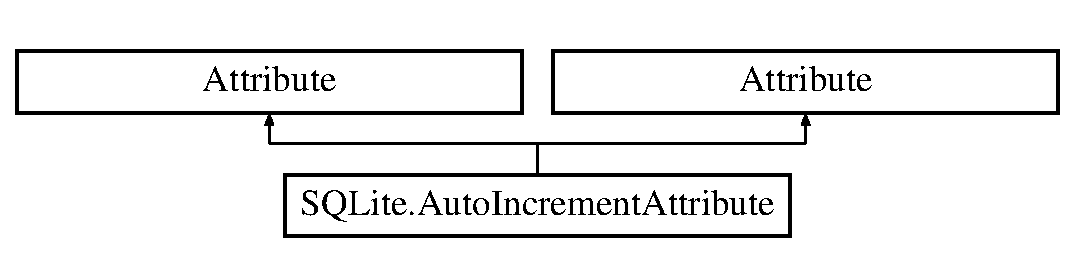
\includegraphics[height=2.000000cm]{classSQLite_1_1AutoIncrementAttribute}
\end{center}
\end{figure}


The documentation for this class was generated from the following file\+:\begin{DoxyCompactItemize}
\item 
packages/sqlite-\/net.\+1.\+0.\+8/content/S\+Q\+Lite.\+cs\end{DoxyCompactItemize}

\hypertarget{classServer_1_1Controllers_1_1APIController_1_1AveragePositionQueue}{\section{Server.\-Controllers.\-A\-P\-I\-Controller.\-Average\-Position\-Queue Class Reference}
\label{classServer_1_1Controllers_1_1APIController_1_1AveragePositionQueue}\index{Server.\-Controllers.\-A\-P\-I\-Controller.\-Average\-Position\-Queue@{Server.\-Controllers.\-A\-P\-I\-Controller.\-Average\-Position\-Queue}}
}


An Class which provides an queue with an position. It is used to avoid threading collisions.  


\subsection*{Public Attributes}
\begin{DoxyCompactItemize}
\item 
\hypertarget{classServer_1_1Controllers_1_1APIController_1_1AveragePositionQueue_afe0ce38ffb7112888253f2047cb62260}{int {\bfseries Count} = 0}\label{classServer_1_1Controllers_1_1APIController_1_1AveragePositionQueue_afe0ce38ffb7112888253f2047cb62260}

\item 
\hypertarget{classServer_1_1Controllers_1_1APIController_1_1AveragePositionQueue_ad97233578791c4725b31c4b873c1b52e}{\hyperlink{classCore_1_1Models_1_1Position}{Core.\-Models.\-Position} {\bfseries Average}}\label{classServer_1_1Controllers_1_1APIController_1_1AveragePositionQueue_ad97233578791c4725b31c4b873c1b52e}

\item 
\hypertarget{classServer_1_1Controllers_1_1APIController_1_1AveragePositionQueue_ad6170762b6e4b77d8c1f09342080cb46}{Mutex {\bfseries Lock}}\label{classServer_1_1Controllers_1_1APIController_1_1AveragePositionQueue_ad6170762b6e4b77d8c1f09342080cb46}

\item 
\hypertarget{classServer_1_1Controllers_1_1APIController_1_1AveragePositionQueue_ac983e9072abb8aab90f443f9bccaf231}{Queue$<$ \hyperlink{classCore_1_1Models_1_1Action}{Core.\-Models.\-Action} $>$ {\bfseries Queue}}\label{classServer_1_1Controllers_1_1APIController_1_1AveragePositionQueue_ac983e9072abb8aab90f443f9bccaf231}

\end{DoxyCompactItemize}


\subsection{Detailed Description}
An Class which provides an queue with an position. It is used to avoid threading collisions. 



The documentation for this class was generated from the following file\-:\begin{DoxyCompactItemize}
\item 
server/\-Controllers/A\-P\-I\-Controller.\-cs\end{DoxyCompactItemize}

\hypertarget{classSQLite_1_1BaseTableQuery}{\section{S\-Q\-Lite.\-Base\-Table\-Query Class Reference}
\label{classSQLite_1_1BaseTableQuery}\index{S\-Q\-Lite.\-Base\-Table\-Query@{S\-Q\-Lite.\-Base\-Table\-Query}}
}
Inheritance diagram for S\-Q\-Lite.\-Base\-Table\-Query\-:\begin{figure}[H]
\begin{center}
\leavevmode
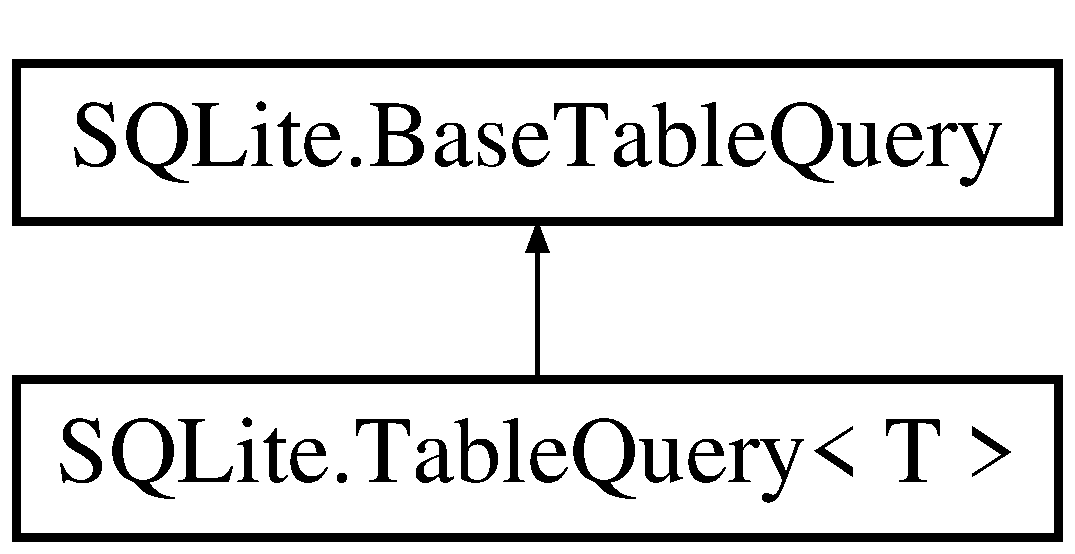
\includegraphics[height=2.000000cm]{classSQLite_1_1BaseTableQuery}
\end{center}
\end{figure}
\subsection*{Classes}
\begin{DoxyCompactItemize}
\item 
class \hyperlink{classSQLite_1_1BaseTableQuery_1_1Ordering}{Ordering}
\end{DoxyCompactItemize}


The documentation for this class was generated from the following file\-:\begin{DoxyCompactItemize}
\item 
packages/sqlite-\/net.\-1.\-0.\-8/content/S\-Q\-Lite.\-cs\end{DoxyCompactItemize}

\hypertarget{classCore_1_1Models_1_1CellPosition}{\section{Core.\-Models.\-Cell\-Position Class Reference}
\label{classCore_1_1Models_1_1CellPosition}\index{Core.\-Models.\-Cell\-Position@{Core.\-Models.\-Cell\-Position}}
}


Represents the cell\-Position in a region. Can be only as large as the region.  


Inheritance diagram for Core.\-Models.\-Cell\-Position\-:\begin{figure}[H]
\begin{center}
\leavevmode
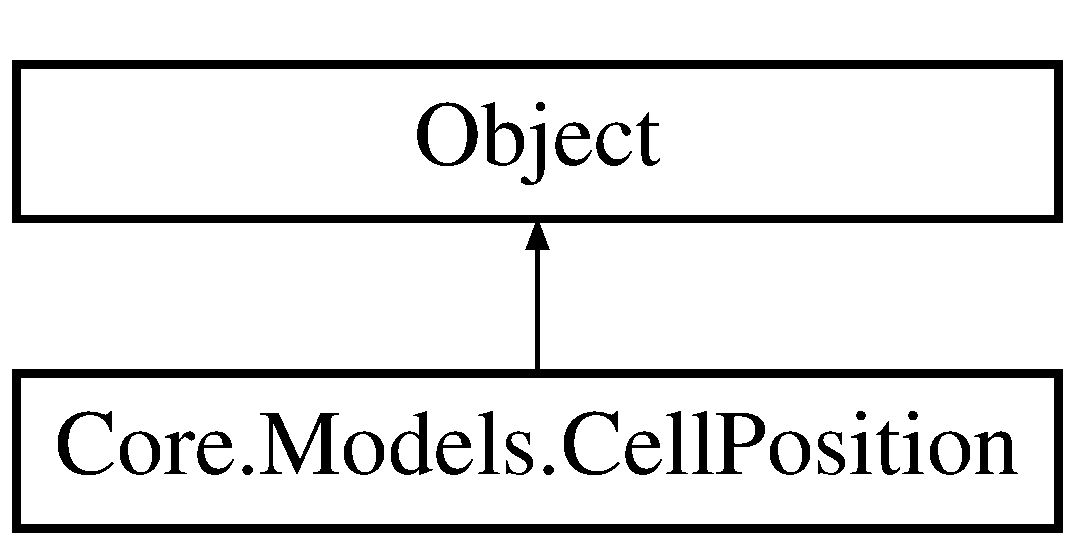
\includegraphics[height=2.000000cm]{classCore_1_1Models_1_1CellPosition}
\end{center}
\end{figure}
\subsection*{Public Member Functions}
\begin{DoxyCompactItemize}
\item 
\hypertarget{classCore_1_1Models_1_1CellPosition_a41b20ccc07f94d036b2aafe9e1830aff}{{\bfseries Cell\-Position} (int cell\-X, int cell\-Y)}\label{classCore_1_1Models_1_1CellPosition_a41b20ccc07f94d036b2aafe9e1830aff}

\item 
\hypertarget{classCore_1_1Models_1_1CellPosition_a6ed85706fc84bcfd93af2efddfebe968}{{\bfseries Cell\-Position} (\hyperlink{classCore_1_1Models_1_1Position}{Position} position)}\label{classCore_1_1Models_1_1CellPosition_a6ed85706fc84bcfd93af2efddfebe968}

\item 
\hypertarget{classCore_1_1Models_1_1CellPosition_ae5a3eb2be34e2e06b8c0addc808e902e}{{\bfseries Cell\-Position} (\hyperlink{classCore_1_1Models_1_1PositionI}{Position\-I} position)}\label{classCore_1_1Models_1_1CellPosition_ae5a3eb2be34e2e06b8c0addc808e902e}

\item 
\hypertarget{classCore_1_1Models_1_1CellPosition_a13d336fb05024daba699cdfb71bd9df2}{{\bfseries Cell\-Position} (J\-Container obj)}\label{classCore_1_1Models_1_1CellPosition_a13d336fb05024daba699cdfb71bd9df2}

\item 
\hypertarget{classCore_1_1Models_1_1CellPosition_afa3430bbcfc6b9a0bcf9340765773658}{override bool {\bfseries Equals} (Object obj)}\label{classCore_1_1Models_1_1CellPosition_afa3430bbcfc6b9a0bcf9340765773658}

\item 
\hypertarget{classCore_1_1Models_1_1CellPosition_a29ab23b29f230954c4277b0f9ad74000}{override int {\bfseries Get\-Hash\-Code} ()}\label{classCore_1_1Models_1_1CellPosition_a29ab23b29f230954c4277b0f9ad74000}

\end{DoxyCompactItemize}
\subsection*{Static Public Member Functions}
\begin{DoxyCompactItemize}
\item 
\hypertarget{classCore_1_1Models_1_1CellPosition_ab477073a5c715c0d25fa2499c7c9582f}{static bool {\bfseries operator==} (\hyperlink{classCore_1_1Models_1_1CellPosition}{Cell\-Position} obj, \hyperlink{classCore_1_1Models_1_1CellPosition}{Cell\-Position} obj2)}\label{classCore_1_1Models_1_1CellPosition_ab477073a5c715c0d25fa2499c7c9582f}

\item 
\hypertarget{classCore_1_1Models_1_1CellPosition_a922b6be828c0a7fa2fe1f340854d3d6f}{static bool {\bfseries operator!=} (\hyperlink{classCore_1_1Models_1_1CellPosition}{Cell\-Position} obj, \hyperlink{classCore_1_1Models_1_1CellPosition}{Cell\-Position} obj2)}\label{classCore_1_1Models_1_1CellPosition_a922b6be828c0a7fa2fe1f340854d3d6f}

\end{DoxyCompactItemize}
\subsection*{Properties}
\begin{DoxyCompactItemize}
\item 
\hypertarget{classCore_1_1Models_1_1CellPosition_a4daf526cdfe22a21d679d3e1b032d096}{int {\bfseries Cell\-X}\hspace{0.3cm}{\ttfamily  \mbox{[}get, set\mbox{]}}}\label{classCore_1_1Models_1_1CellPosition_a4daf526cdfe22a21d679d3e1b032d096}

\item 
\hypertarget{classCore_1_1Models_1_1CellPosition_a91ba33cce7deac7d2ec875812c3f73dc}{int {\bfseries Cell\-Y}\hspace{0.3cm}{\ttfamily  \mbox{[}get, set\mbox{]}}}\label{classCore_1_1Models_1_1CellPosition_a91ba33cce7deac7d2ec875812c3f73dc}

\end{DoxyCompactItemize}


\subsection{Detailed Description}
Represents the cell\-Position in a region. Can be only as large as the region. 



The documentation for this class was generated from the following file\-:\begin{DoxyCompactItemize}
\item 
base/\-Models/\-Position/Cell\-Position.\-cs\end{DoxyCompactItemize}

\hypertarget{classClient_1_1Common_1_1Helper_1_1ClientConstants}{\section{Client.\-Common.\-Helper.\-Client\-Constants Class Reference}
\label{classClient_1_1Common_1_1Helper_1_1ClientConstants}\index{Client.\-Common.\-Helper.\-Client\-Constants@{Client.\-Common.\-Helper.\-Client\-Constants}}
}
\subsection*{Public Attributes}
\begin{DoxyCompactItemize}
\item 
\hypertarget{classClient_1_1Common_1_1Helper_1_1ClientConstants_a0c4448ce7b1a345e18f40fb7f1c963c7}{const string {\bfseries C\-O\-N\-T\-E\-N\-T} = \char`\"{}Content\char`\"{}}\label{classClient_1_1Common_1_1Helper_1_1ClientConstants_a0c4448ce7b1a345e18f40fb7f1c963c7}

\item 
\hypertarget{classClient_1_1Common_1_1Helper_1_1ClientConstants_a60ef84449ad577edc5a9271ff579ba8f}{const string {\bfseries A\-N\-I\-M\-A\-T\-I\-O\-N\-S} = \char`\"{}animations\char`\"{}}\label{classClient_1_1Common_1_1Helper_1_1ClientConstants_a60ef84449ad577edc5a9271ff579ba8f}

\item 
\hypertarget{classClient_1_1Common_1_1Helper_1_1ClientConstants_a52c908ccd26ad80c739e26faaebf5a5c}{const string {\bfseries F\-O\-N\-T\-S} = \char`\"{}fonts\char`\"{}}\label{classClient_1_1Common_1_1Helper_1_1ClientConstants_a52c908ccd26ad80c739e26faaebf5a5c}

\item 
\hypertarget{classClient_1_1Common_1_1Helper_1_1ClientConstants_acccad18fa5b18e5e42bda30a778883be}{const string {\bfseries S\-O\-U\-N\-D\-S} = \char`\"{}sounds\char`\"{}}\label{classClient_1_1Common_1_1Helper_1_1ClientConstants_acccad18fa5b18e5e42bda30a778883be}

\item 
\hypertarget{classClient_1_1Common_1_1Helper_1_1ClientConstants_a73802f084c13346a0b9f747aade18b01}{const string {\bfseries T\-I\-L\-E\-S} = \char`\"{}tiles\char`\"{}}\label{classClient_1_1Common_1_1Helper_1_1ClientConstants_a73802f084c13346a0b9f747aade18b01}

\item 
\hypertarget{classClient_1_1Common_1_1Helper_1_1ClientConstants_a1ffb72ae453b43952c3ced93de626a15}{const string {\bfseries I\-M\-A\-G\-E\-S} = \char`\"{}images\char`\"{}}\label{classClient_1_1Common_1_1Helper_1_1ClientConstants_a1ffb72ae453b43952c3ced93de626a15}

\item 
\hypertarget{classClient_1_1Common_1_1Helper_1_1ClientConstants_aa1a5b1c5317bc476a4357e1d8e769df5}{const string {\bfseries I\-M\-A\-G\-E\-S\-\_\-\-H\-D} = \char`\"{}images/hd\char`\"{}}\label{classClient_1_1Common_1_1Helper_1_1ClientConstants_aa1a5b1c5317bc476a4357e1d8e769df5}

\item 
\hypertarget{classClient_1_1Common_1_1Helper_1_1ClientConstants_ac08b4c199c1811502d8a4fb6e7c110c4}{const string {\bfseries I\-M\-A\-G\-E\-S\-\_\-\-L\-D} = \char`\"{}images/ld\char`\"{}}\label{classClient_1_1Common_1_1Helper_1_1ClientConstants_ac08b4c199c1811502d8a4fb6e7c110c4}

\item 
\hypertarget{classClient_1_1Common_1_1Helper_1_1ClientConstants_af933c866a55d35d67506082c502b176e}{const string {\bfseries L\-O\-G\-I\-C\-\_\-\-S\-E\-R\-V\-E\-R} = \char`\"{}http\-://derfalke.\-no-\/ip.\-biz\-:9000\char`\"{}}\label{classClient_1_1Common_1_1Helper_1_1ClientConstants_af933c866a55d35d67506082c502b176e}

\item 
\hypertarget{classClient_1_1Common_1_1Helper_1_1ClientConstants_a7c994023c157ac2c31b9b5c67ee15f6f}{const string {\bfseries D\-A\-T\-A\-\_\-\-S\-E\-R\-V\-E\-R} = \char`\"{}http\-://derfalke.\-no-\/ip.\-biz\char`\"{}}\label{classClient_1_1Common_1_1Helper_1_1ClientConstants_a7c994023c157ac2c31b9b5c67ee15f6f}

\item 
\hypertarget{classClient_1_1Common_1_1Helper_1_1ClientConstants_aa74dab28e1bd4c782ce69c777bf11b18}{const string {\bfseries R\-E\-G\-I\-O\-N\-\_\-\-S\-E\-R\-V\-E\-R\-\_\-\-P\-A\-T\-H} = D\-A\-T\-A\-\_\-\-S\-E\-R\-V\-E\-R + \char`\"{}/world/\$Major\-Region\-X/\$Major\-Region\-Y/germany-\/\$Minor\-Region\-X-\/\$Minor\-Region\-Y.\-json\char`\"{}}\label{classClient_1_1Common_1_1Helper_1_1ClientConstants_aa74dab28e1bd4c782ce69c777bf11b18}

\item 
\hypertarget{classClient_1_1Common_1_1Helper_1_1ClientConstants_a9cf3c4ead310b5fd6e58c18f0e09d175}{const string {\bfseries U\-N\-I\-T\-\_\-\-T\-Y\-P\-E\-S\-\_\-\-S\-E\-R\-V\-E\-R\-\_\-\-P\-A\-T\-H} = D\-A\-T\-A\-\_\-\-S\-E\-R\-V\-E\-R + \char`\"{}/unit.\-json\char`\"{}}\label{classClient_1_1Common_1_1Helper_1_1ClientConstants_a9cf3c4ead310b5fd6e58c18f0e09d175}

\item 
\hypertarget{classClient_1_1Common_1_1Helper_1_1ClientConstants_a2d74341dc9307aaa6a6601442898ec07}{const string {\bfseries T\-E\-R\-R\-A\-I\-N\-\_\-\-T\-Y\-P\-E\-S\-\_\-\-S\-E\-R\-V\-E\-R\-\_\-\-P\-A\-T\-H} = D\-A\-T\-A\-\_\-\-S\-E\-R\-V\-E\-R + \char`\"{}/terrain.\-json\char`\"{}}\label{classClient_1_1Common_1_1Helper_1_1ClientConstants_a2d74341dc9307aaa6a6601442898ec07}

\item 
\hypertarget{classClient_1_1Common_1_1Helper_1_1ClientConstants_a54709bc353b9c204d6c9649ff76de5cb}{const string {\bfseries L\-O\-G\-I\-N\-\_\-\-P\-A\-T\-H} = L\-O\-G\-I\-C\-\_\-\-S\-E\-R\-V\-E\-R + \char`\"{}/Login?json=\$J\-S\-O\-N\char`\"{}}\label{classClient_1_1Common_1_1Helper_1_1ClientConstants_a54709bc353b9c204d6c9649ff76de5cb}

\item 
\hypertarget{classClient_1_1Common_1_1Helper_1_1ClientConstants_adb27b1857784ed0d60bde8d7be06fce2}{const string {\bfseries L\-O\-A\-D\-\_\-\-R\-E\-G\-I\-O\-N\-S\-\_\-\-P\-A\-T\-H} = L\-O\-G\-I\-C\-\_\-\-S\-E\-R\-V\-E\-R + \char`\"{}/Load\-Regions?json=\$J\-S\-O\-N\char`\"{}}\label{classClient_1_1Common_1_1Helper_1_1ClientConstants_adb27b1857784ed0d60bde8d7be06fce2}

\item 
\hypertarget{classClient_1_1Common_1_1Helper_1_1ClientConstants_a288cdae05f5b0efa041eb10ed5d5b693}{const string {\bfseries D\-O\-\_\-\-A\-C\-T\-I\-O\-N\-S\-\_\-\-P\-A\-T\-H} = L\-O\-G\-I\-C\-\_\-\-S\-E\-R\-V\-E\-R + \char`\"{}/Do\-Actions?json=\$J\-S\-O\-N\char`\"{}}\label{classClient_1_1Common_1_1Helper_1_1ClientConstants_a288cdae05f5b0efa041eb10ed5d5b693}

\item 
\hypertarget{classClient_1_1Common_1_1Helper_1_1ClientConstants_ae0f3b5d21066fa553b3173acba49a0d9}{const string {\bfseries L\-O\-G\-I\-C\-\_\-\-S\-E\-R\-V\-E\-R\-\_\-\-J\-S\-O\-N} = \char`\"{}\$J\-S\-O\-N\char`\"{}}\label{classClient_1_1Common_1_1Helper_1_1ClientConstants_ae0f3b5d21066fa553b3173acba49a0d9}

\item 
\hypertarget{classClient_1_1Common_1_1Helper_1_1ClientConstants_a5d50b38f09c095e2634a22d1104126b1}{const int {\bfseries C\-E\-L\-L\-M\-A\-P\-\_\-160x160\-\_\-\-S\-I\-Z\-E} = 160}\label{classClient_1_1Common_1_1Helper_1_1ClientConstants_a5d50b38f09c095e2634a22d1104126b1}

\item 
\hypertarget{classClient_1_1Common_1_1Helper_1_1ClientConstants_a7fd36de3c05426f7a5ec6abda4467ffd}{const string {\bfseries T\-I\-L\-E\-M\-A\-P\-\_\-\-F\-I\-L\-E} = \char`\"{}Worldmap-\/160x160(80x320)\-\_\-20150704\char`\"{}}\label{classClient_1_1Common_1_1Helper_1_1ClientConstants_a7fd36de3c05426f7a5ec6abda4467ffd}

\item 
\hypertarget{classClient_1_1Common_1_1Helper_1_1ClientConstants_ad5629033db14bd9fe132847af3daed00}{const string {\bfseries L\-A\-Y\-E\-R\-\_\-\-T\-E\-R\-R\-A\-I\-N} = \char`\"{}Layer 0\char`\"{}}\label{classClient_1_1Common_1_1Helper_1_1ClientConstants_ad5629033db14bd9fe132847af3daed00}

\item 
\hypertarget{classClient_1_1Common_1_1Helper_1_1ClientConstants_a1b84622eb7022993d92289cb920d98c8}{const string {\bfseries L\-A\-Y\-E\-R\-\_\-\-B\-U\-I\-L\-D\-I\-N\-G} = \char`\"{}Layer 1\char`\"{}}\label{classClient_1_1Common_1_1Helper_1_1ClientConstants_a1b84622eb7022993d92289cb920d98c8}

\item 
\hypertarget{classClient_1_1Common_1_1Helper_1_1ClientConstants_a40aa439b73a837494df742222456c7e0}{const string {\bfseries L\-A\-Y\-E\-R\-\_\-\-U\-N\-I\-T} = \char`\"{}Layer 2\char`\"{}}\label{classClient_1_1Common_1_1Helper_1_1ClientConstants_a40aa439b73a837494df742222456c7e0}

\item 
\hypertarget{classClient_1_1Common_1_1Helper_1_1ClientConstants_afec2990249ac95db28f06ce2c36cfd1e}{const string {\bfseries L\-A\-Y\-E\-R\-\_\-\-M\-E\-N\-U} = \char`\"{}Layer 3\char`\"{}}\label{classClient_1_1Common_1_1Helper_1_1ClientConstants_afec2990249ac95db28f06ce2c36cfd1e}

\item 
\hypertarget{classClient_1_1Common_1_1Helper_1_1ClientConstants_ac9d959187b42417e5eed13631f5d6a0e}{const float {\bfseries T\-I\-L\-E\-\_\-\-I\-M\-A\-G\-E\-\_\-\-W\-I\-D\-T\-H} = 83.\-0f}\label{classClient_1_1Common_1_1Helper_1_1ClientConstants_ac9d959187b42417e5eed13631f5d6a0e}

\item 
\hypertarget{classClient_1_1Common_1_1Helper_1_1ClientConstants_a35a4dc018d8f3c033f9f81bc370a4bbf}{const int {\bfseries T\-I\-L\-E\-M\-A\-P\-\_\-\-W\-I\-D\-T\-H} = 80}\label{classClient_1_1Common_1_1Helper_1_1ClientConstants_a35a4dc018d8f3c033f9f81bc370a4bbf}

\item 
\hypertarget{classClient_1_1Common_1_1Helper_1_1ClientConstants_ad117e0e9ea54dbf283440fc78575dc61}{const int {\bfseries T\-I\-L\-E\-M\-A\-P\-\_\-\-H\-I\-G\-H} = 320}\label{classClient_1_1Common_1_1Helper_1_1ClientConstants_ad117e0e9ea54dbf283440fc78575dc61}

\item 
\hypertarget{classClient_1_1Common_1_1Helper_1_1ClientConstants_ada0ea4ee3b8c36532c145ff3cb0aada9}{const float {\bfseries T\-I\-L\-E\-M\-A\-P\-\_\-\-M\-I\-N\-\_\-\-S\-C\-A\-L\-E} = 0.\-3f}\label{classClient_1_1Common_1_1Helper_1_1ClientConstants_ada0ea4ee3b8c36532c145ff3cb0aada9}

\item 
\hypertarget{classClient_1_1Common_1_1Helper_1_1ClientConstants_a2372f52b5744ca9dc71b2b7232c6ee02}{const float {\bfseries T\-I\-L\-E\-M\-A\-P\-\_\-\-N\-O\-R\-M\-\_\-\-S\-C\-A\-L\-E} = 0.\-5f}\label{classClient_1_1Common_1_1Helper_1_1ClientConstants_a2372f52b5744ca9dc71b2b7232c6ee02}

\item 
\hypertarget{classClient_1_1Common_1_1Helper_1_1ClientConstants_a51a00204c51ce8da99a7dae7a0c9c24b}{const float {\bfseries T\-I\-L\-E\-M\-A\-P\-\_\-\-M\-A\-X\-\_\-\-S\-C\-A\-L\-E} = 3.\-0f}\label{classClient_1_1Common_1_1Helper_1_1ClientConstants_a51a00204c51ce8da99a7dae7a0c9c24b}

\item 
\hypertarget{classClient_1_1Common_1_1Helper_1_1ClientConstants_a05829491ea18162cd8b7a71640d949d4}{const short {\bfseries D\-R\-A\-W\-\_\-\-R\-E\-G\-I\-O\-N\-S\-\_\-\-X} = 5}\label{classClient_1_1Common_1_1Helper_1_1ClientConstants_a05829491ea18162cd8b7a71640d949d4}

\item 
\hypertarget{classClient_1_1Common_1_1Helper_1_1ClientConstants_a87f7ef3a586370c92e7165a19dc17c9e}{const short {\bfseries D\-R\-A\-W\-\_\-\-R\-E\-G\-I\-O\-N\-S\-\_\-\-Y} = 5}\label{classClient_1_1Common_1_1Helper_1_1ClientConstants_a87f7ef3a586370c92e7165a19dc17c9e}

\item 
\hypertarget{classClient_1_1Common_1_1Helper_1_1ClientConstants_ab15618493a1b3c441b454ad75afad02e}{const double {\bfseries R\-E\-D\-R\-A\-W\-\_\-\-R\-E\-G\-I\-O\-N\-S\-\_\-\-S\-T\-A\-R\-T\-\_\-\-X} = 1.\-5 $\ast$ Core.\-Models.\-Constants.\-R\-E\-G\-I\-O\-N\-\_\-\-S\-I\-Z\-E\-\_\-\-X}\label{classClient_1_1Common_1_1Helper_1_1ClientConstants_ab15618493a1b3c441b454ad75afad02e}

\item 
\hypertarget{classClient_1_1Common_1_1Helper_1_1ClientConstants_a989f3decc8372888fd282eab3be1d768}{const double {\bfseries R\-E\-D\-R\-A\-W\-\_\-\-R\-E\-G\-I\-O\-N\-S\-\_\-\-E\-N\-D\-\_\-\-X} = 3.\-5 $\ast$ Core.\-Models.\-Constants.\-R\-E\-G\-I\-O\-N\-\_\-\-S\-I\-Z\-E\-\_\-\-X}\label{classClient_1_1Common_1_1Helper_1_1ClientConstants_a989f3decc8372888fd282eab3be1d768}

\item 
\hypertarget{classClient_1_1Common_1_1Helper_1_1ClientConstants_afd8772b1bfbfea0b0ed22e5b224c7744}{const double {\bfseries R\-E\-D\-R\-A\-W\-\_\-\-R\-E\-G\-I\-O\-N\-S\-\_\-\-S\-T\-A\-R\-T\-\_\-\-Y} = 1.\-5 $\ast$ Core.\-Models.\-Constants.\-R\-E\-G\-I\-O\-N\-\_\-\-S\-I\-Z\-E\-\_\-\-Y}\label{classClient_1_1Common_1_1Helper_1_1ClientConstants_afd8772b1bfbfea0b0ed22e5b224c7744}

\item 
\hypertarget{classClient_1_1Common_1_1Helper_1_1ClientConstants_ab33ebb3b8725c3ab0b34e7b330b484ec}{const double {\bfseries R\-E\-D\-R\-A\-W\-\_\-\-R\-E\-G\-I\-O\-N\-S\-\_\-\-E\-N\-D\-\_\-\-Y} = 3.\-5 $\ast$ Core.\-Models.\-Constants.\-R\-E\-G\-I\-O\-N\-\_\-\-S\-I\-Z\-E\-\_\-\-Y}\label{classClient_1_1Common_1_1Helper_1_1ClientConstants_ab33ebb3b8725c3ab0b34e7b330b484ec}

\item 
\hypertarget{classClient_1_1Common_1_1Helper_1_1ClientConstants_aedbbdef3e335ce3cb95e5276784220ad}{const short {\bfseries W\-A\-T\-E\-R\-\_\-\-G\-I\-D} = 10}\label{classClient_1_1Common_1_1Helper_1_1ClientConstants_aedbbdef3e335ce3cb95e5276784220ad}

\item 
\hypertarget{classClient_1_1Common_1_1Helper_1_1ClientConstants_a2e2b55c5e761acd466b9b62a2cb4f485}{const short {\bfseries B\-U\-I\-L\-D\-I\-N\-G\-S\-\_\-\-G\-I\-D} = 7}\label{classClient_1_1Common_1_1Helper_1_1ClientConstants_a2e2b55c5e761acd466b9b62a2cb4f485}

\item 
\hypertarget{classClient_1_1Common_1_1Helper_1_1ClientConstants_a001ddcc224f28b7b0390e95d1f64ef7b}{const short {\bfseries W\-O\-O\-D\-S\-\_\-\-G\-I\-D} = 9}\label{classClient_1_1Common_1_1Helper_1_1ClientConstants_a001ddcc224f28b7b0390e95d1f64ef7b}

\item 
\hypertarget{classClient_1_1Common_1_1Helper_1_1ClientConstants_ac0fdbf4905a52399d6a9eee737a5fc0d}{const short {\bfseries G\-R\-A\-S\-S\-L\-A\-N\-D\-\_\-\-G\-I\-D} = 5}\label{classClient_1_1Common_1_1Helper_1_1ClientConstants_ac0fdbf4905a52399d6a9eee737a5fc0d}

\item 
\hypertarget{classClient_1_1Common_1_1Helper_1_1ClientConstants_a0bb306f4e18e5f103f0f1ccb8f47493c}{const short {\bfseries F\-I\-E\-L\-D\-S\-\_\-\-G\-I\-D} = 3}\label{classClient_1_1Common_1_1Helper_1_1ClientConstants_a0bb306f4e18e5f103f0f1ccb8f47493c}

\item 
\hypertarget{classClient_1_1Common_1_1Helper_1_1ClientConstants_a7f8eeabec8f614cdd5421cb18ba0b338}{const short {\bfseries S\-T\-R\-E\-E\-T\-S\-\_\-\-G\-I\-D} = 8}\label{classClient_1_1Common_1_1Helper_1_1ClientConstants_a7f8eeabec8f614cdd5421cb18ba0b338}

\item 
\hypertarget{classClient_1_1Common_1_1Helper_1_1ClientConstants_a8899d1c0fb41d68e759afc26aae10c85}{const short {\bfseries N\-O\-T\-D\-E\-F\-I\-N\-E\-D\-\_\-\-G\-I\-D} = 1}\label{classClient_1_1Common_1_1Helper_1_1ClientConstants_a8899d1c0fb41d68e759afc26aae10c85}

\item 
\hypertarget{classClient_1_1Common_1_1Helper_1_1ClientConstants_a5c55c571f481ad97920844cf444111f8}{const short {\bfseries F\-O\-R\-B\-I\-D\-D\-E\-N\-\_\-\-G\-I\-D} = 1}\label{classClient_1_1Common_1_1Helper_1_1ClientConstants_a5c55c571f481ad97920844cf444111f8}

\item 
\hypertarget{classClient_1_1Common_1_1Helper_1_1ClientConstants_abb743cbc03bdea03d7d13ce2c4842b81}{const short {\bfseries T\-O\-W\-N\-\_\-\-G\-I\-D} = 6}\label{classClient_1_1Common_1_1Helper_1_1ClientConstants_abb743cbc03bdea03d7d13ce2c4842b81}

\item 
\hypertarget{classClient_1_1Common_1_1Helper_1_1ClientConstants_aae2c70715b5b7c06d43b291f841ce26c}{const short {\bfseries G\-L\-A\-C\-I\-E\-R\-\_\-\-G\-I\-D} = 4}\label{classClient_1_1Common_1_1Helper_1_1ClientConstants_aae2c70715b5b7c06d43b291f841ce26c}

\item 
\hypertarget{classClient_1_1Common_1_1Helper_1_1ClientConstants_ace18b796f7870c06429a6abe99319ae9}{const short {\bfseries B\-E\-A\-C\-H\-\_\-\-G\-I\-D} = 2}\label{classClient_1_1Common_1_1Helper_1_1ClientConstants_ace18b796f7870c06429a6abe99319ae9}

\item 
\hypertarget{classClient_1_1Common_1_1Helper_1_1ClientConstants_acb903f1f95fb70e6469f2e20fb6a0336}{const short {\bfseries P\-A\-R\-K\-\_\-\-G\-I\-D} = 11}\label{classClient_1_1Common_1_1Helper_1_1ClientConstants_acb903f1f95fb70e6469f2e20fb6a0336}

\item 
\hypertarget{classClient_1_1Common_1_1Helper_1_1ClientConstants_a4c33195c698395a632541bd1ec334080}{const short {\bfseries I\-N\-V\-A\-L\-I\-D\-\_\-\-G\-I\-D} = 1}\label{classClient_1_1Common_1_1Helper_1_1ClientConstants_a4c33195c698395a632541bd1ec334080}

\item 
\hypertarget{classClient_1_1Common_1_1Helper_1_1ClientConstants_aa951367db63113c16fc1363f4168dce7}{const short {\bfseries B\-O\-W\-M\-A\-N\-\_\-\-G\-I\-D} = 46}\label{classClient_1_1Common_1_1Helper_1_1ClientConstants_aa951367db63113c16fc1363f4168dce7}

\item 
\hypertarget{classClient_1_1Common_1_1Helper_1_1ClientConstants_a399cb2b8499e96b0fbaff7125a8b0758}{const short {\bfseries H\-E\-R\-O\-\_\-\-G\-I\-D} = 47}\label{classClient_1_1Common_1_1Helper_1_1ClientConstants_a399cb2b8499e96b0fbaff7125a8b0758}

\item 
\hypertarget{classClient_1_1Common_1_1Helper_1_1ClientConstants_aed51652c0aee9f4d1c979b74ccc8e4cc}{const short {\bfseries W\-A\-R\-R\-I\-O\-R\-\_\-\-G\-I\-D} = 48}\label{classClient_1_1Common_1_1Helper_1_1ClientConstants_aed51652c0aee9f4d1c979b74ccc8e4cc}

\item 
\hypertarget{classClient_1_1Common_1_1Helper_1_1ClientConstants_a4622cdf352112a7961b9bfa98cba098d}{const short {\bfseries M\-A\-G\-E\-\_\-\-G\-I\-D} = 49}\label{classClient_1_1Common_1_1Helper_1_1ClientConstants_a4622cdf352112a7961b9bfa98cba098d}

\item 
\hypertarget{classClient_1_1Common_1_1Helper_1_1ClientConstants_a1a477548296662496e6d73a9effa5729}{const short {\bfseries S\-C\-O\-U\-T\-\_\-\-G\-I\-D} = 50}\label{classClient_1_1Common_1_1Helper_1_1ClientConstants_a1a477548296662496e6d73a9effa5729}

\item 
\hypertarget{classClient_1_1Common_1_1Helper_1_1ClientConstants_a24d643ac5ef0c684a0139e70b2ab3c17}{const short {\bfseries U\-N\-K\-N\-O\-W\-N\-\_\-\-G\-I\-D} = 51}\label{classClient_1_1Common_1_1Helper_1_1ClientConstants_a24d643ac5ef0c684a0139e70b2ab3c17}

\item 
\hypertarget{classClient_1_1Common_1_1Helper_1_1ClientConstants_acab54073e4ed018d8f81715e60de1ea3}{const short {\bfseries M\-E\-N\-U\-E\-B\-O\-W\-M\-A\-N\-\_\-\-G\-I\-D} = 60}\label{classClient_1_1Common_1_1Helper_1_1ClientConstants_acab54073e4ed018d8f81715e60de1ea3}

\item 
\hypertarget{classClient_1_1Common_1_1Helper_1_1ClientConstants_a701e21642a3bb3a450b2b65195aaf75e}{const short {\bfseries M\-E\-N\-U\-E\-H\-E\-R\-O\-\_\-\-G\-I\-D} = 61}\label{classClient_1_1Common_1_1Helper_1_1ClientConstants_a701e21642a3bb3a450b2b65195aaf75e}

\item 
\hypertarget{classClient_1_1Common_1_1Helper_1_1ClientConstants_a6fabb2c7e1eed7bee4fea2b92a1b8511}{const short {\bfseries M\-E\-N\-U\-E\-W\-A\-R\-R\-I\-O\-R\-\_\-\-G\-I\-D} = 62}\label{classClient_1_1Common_1_1Helper_1_1ClientConstants_a6fabb2c7e1eed7bee4fea2b92a1b8511}

\item 
\hypertarget{classClient_1_1Common_1_1Helper_1_1ClientConstants_a9bc1306e327dccf1d431e0d4f09f4b38}{const short {\bfseries M\-E\-N\-U\-E\-M\-A\-G\-E\-\_\-\-G\-I\-D} = 63}\label{classClient_1_1Common_1_1Helper_1_1ClientConstants_a9bc1306e327dccf1d431e0d4f09f4b38}

\item 
\hypertarget{classClient_1_1Common_1_1Helper_1_1ClientConstants_aa9da5c5ad1598ea7958d428179869a5c}{const short {\bfseries M\-E\-N\-U\-E\-S\-C\-O\-U\-T\-\_\-\-G\-I\-D} = 64}\label{classClient_1_1Common_1_1Helper_1_1ClientConstants_aa9da5c5ad1598ea7958d428179869a5c}

\item 
\hypertarget{classClient_1_1Common_1_1Helper_1_1ClientConstants_aad55692d6d0ac6f6df14ec043252704a}{const short {\bfseries M\-E\-N\-U\-E\-U\-N\-K\-N\-O\-W\-N\-\_\-\-G\-I\-D} = 65}\label{classClient_1_1Common_1_1Helper_1_1ClientConstants_aad55692d6d0ac6f6df14ec043252704a}

\item 
\hypertarget{classClient_1_1Common_1_1Helper_1_1ClientConstants_ab34e5bc1bdb425e8e376dd7b41138dab}{const short {\bfseries F\-A\-R\-M\-\_\-\-G\-I\-D} = 12}\label{classClient_1_1Common_1_1Helper_1_1ClientConstants_ab34e5bc1bdb425e8e376dd7b41138dab}

\item 
\hypertarget{classClient_1_1Common_1_1Helper_1_1ClientConstants_acf46b35f0f602ede54d355c4cc93a152}{const short {\bfseries G\-A\-R\-N\-I\-S\-I\-O\-N\-\_\-\-G\-I\-D} = 13}\label{classClient_1_1Common_1_1Helper_1_1ClientConstants_acf46b35f0f602ede54d355c4cc93a152}

\item 
\hypertarget{classClient_1_1Common_1_1Helper_1_1ClientConstants_a37ad28f1a65443b021f7992fd2321055}{const short {\bfseries H\-E\-A\-D\-Q\-U\-A\-R\-T\-E\-R\-\_\-\-G\-I\-D} = 14}\label{classClient_1_1Common_1_1Helper_1_1ClientConstants_a37ad28f1a65443b021f7992fd2321055}

\item 
\hypertarget{classClient_1_1Common_1_1Helper_1_1ClientConstants_a73dcc82f6c3a3c80f06c1903cdbc1d5d}{const short {\bfseries H\-O\-U\-S\-E\-\_\-\-G\-I\-D} = 15}\label{classClient_1_1Common_1_1Helper_1_1ClientConstants_a73dcc82f6c3a3c80f06c1903cdbc1d5d}

\item 
\hypertarget{classClient_1_1Common_1_1Helper_1_1ClientConstants_a5ae2aa6a611c67ff7137e5ecb96e410f}{const short {\bfseries T\-O\-W\-E\-R1\-\_\-\-G\-I\-D} = 16}\label{classClient_1_1Common_1_1Helper_1_1ClientConstants_a5ae2aa6a611c67ff7137e5ecb96e410f}

\item 
\hypertarget{classClient_1_1Common_1_1Helper_1_1ClientConstants_a9ea46ffbff17c68a8a4937845d0a03d4}{const short {\bfseries T\-O\-W\-E\-R2\-\_\-\-G\-I\-D} = 17}\label{classClient_1_1Common_1_1Helper_1_1ClientConstants_a9ea46ffbff17c68a8a4937845d0a03d4}

\item 
\hypertarget{classClient_1_1Common_1_1Helper_1_1ClientConstants_afd2c5044a7ec5073888db2f562f83d0c}{const short {\bfseries T\-O\-W\-E\-R3\-\_\-\-G\-I\-D} = 18}\label{classClient_1_1Common_1_1Helper_1_1ClientConstants_afd2c5044a7ec5073888db2f562f83d0c}

\item 
\hypertarget{classClient_1_1Common_1_1Helper_1_1ClientConstants_a3fc94c8d48def9c84f8b31c09f2ef341}{const short {\bfseries T\-O\-W\-E\-R4\-\_\-\-G\-I\-D} = 19}\label{classClient_1_1Common_1_1Helper_1_1ClientConstants_a3fc94c8d48def9c84f8b31c09f2ef341}

\item 
\hypertarget{classClient_1_1Common_1_1Helper_1_1ClientConstants_a04cf17467107ee04378a813b32ccea10}{const short {\bfseries T\-O\-W\-E\-R5\-\_\-\-G\-I\-D} = 20}\label{classClient_1_1Common_1_1Helper_1_1ClientConstants_a04cf17467107ee04378a813b32ccea10}

\item 
\hypertarget{classClient_1_1Common_1_1Helper_1_1ClientConstants_a513abbb0f255e33ad075686b48f40a3c}{const short {\bfseries T\-O\-W\-E\-R6\-\_\-\-G\-I\-D} = 21}\label{classClient_1_1Common_1_1Helper_1_1ClientConstants_a513abbb0f255e33ad075686b48f40a3c}

\item 
\hypertarget{classClient_1_1Common_1_1Helper_1_1ClientConstants_ac3f756c5f55f3ca47b07d6c0a5d2c8b1}{const short {\bfseries W\-A\-L\-L1\-\_\-\-G\-I\-D} = 22}\label{classClient_1_1Common_1_1Helper_1_1ClientConstants_ac3f756c5f55f3ca47b07d6c0a5d2c8b1}

\item 
\hypertarget{classClient_1_1Common_1_1Helper_1_1ClientConstants_a6cffdbb2f9fffd04c1630a70167061bc}{const short {\bfseries W\-A\-L\-L2\-\_\-\-G\-I\-D} = 23}\label{classClient_1_1Common_1_1Helper_1_1ClientConstants_a6cffdbb2f9fffd04c1630a70167061bc}

\item 
\hypertarget{classClient_1_1Common_1_1Helper_1_1ClientConstants_a7cb62ea2940c5e699aae75d9c9e04e97}{const short {\bfseries W\-A\-L\-L3\-\_\-\-G\-I\-D} = 24}\label{classClient_1_1Common_1_1Helper_1_1ClientConstants_a7cb62ea2940c5e699aae75d9c9e04e97}

\item 
\hypertarget{classClient_1_1Common_1_1Helper_1_1ClientConstants_a5d8777e9667b3c74acd5bc9e3b6e864f}{const short {\bfseries W\-A\-L\-L4\-\_\-\-G\-I\-D} = 25}\label{classClient_1_1Common_1_1Helper_1_1ClientConstants_a5d8777e9667b3c74acd5bc9e3b6e864f}

\item 
\hypertarget{classClient_1_1Common_1_1Helper_1_1ClientConstants_a9b7baf114cb37c99a77478dc58e017e0}{const short {\bfseries W\-A\-L\-L5\-\_\-\-G\-I\-D} = 26}\label{classClient_1_1Common_1_1Helper_1_1ClientConstants_a9b7baf114cb37c99a77478dc58e017e0}

\item 
\hypertarget{classClient_1_1Common_1_1Helper_1_1ClientConstants_aae2517b0e11f6beba9dd7bf5db209674}{const short {\bfseries W\-A\-L\-L6\-\_\-\-G\-I\-D} = 27}\label{classClient_1_1Common_1_1Helper_1_1ClientConstants_aae2517b0e11f6beba9dd7bf5db209674}

\item 
\hypertarget{classClient_1_1Common_1_1Helper_1_1ClientConstants_aef8049ceeddd4bec46505a76e57962ee}{const short {\bfseries B\-A\-R\-R\-A\-C\-K\-S\-E\-A\-R\-T\-H\-\_\-\-G\-I\-D} = 34}\label{classClient_1_1Common_1_1Helper_1_1ClientConstants_aef8049ceeddd4bec46505a76e57962ee}

\item 
\hypertarget{classClient_1_1Common_1_1Helper_1_1ClientConstants_aec48a2bde62fc2aa2f7709b073dd5ec0}{const short {\bfseries B\-A\-R\-R\-A\-C\-K\-S\-F\-I\-R\-E\-\_\-\-G\-I\-D} = 35}\label{classClient_1_1Common_1_1Helper_1_1ClientConstants_aec48a2bde62fc2aa2f7709b073dd5ec0}

\item 
\hypertarget{classClient_1_1Common_1_1Helper_1_1ClientConstants_a3174357a8e4874dae5c4d53a25a8bb39}{const short {\bfseries B\-A\-R\-R\-A\-C\-K\-S\-G\-O\-L\-D\-\_\-\-G\-I\-D} = 36}\label{classClient_1_1Common_1_1Helper_1_1ClientConstants_a3174357a8e4874dae5c4d53a25a8bb39}

\item 
\hypertarget{classClient_1_1Common_1_1Helper_1_1ClientConstants_a857b6ba4bbc64843443378acf473542d}{const short {\bfseries B\-A\-R\-R\-A\-C\-K\-S\-A\-I\-R\-\_\-\-G\-I\-D} = 37}\label{classClient_1_1Common_1_1Helper_1_1ClientConstants_a857b6ba4bbc64843443378acf473542d}

\item 
\hypertarget{classClient_1_1Common_1_1Helper_1_1ClientConstants_a3434cc51db28e4f158f16d4a21971d5f}{const short {\bfseries B\-A\-R\-R\-A\-C\-K\-S\-M\-A\-G\-I\-C\-\_\-\-G\-I\-D} = 38}\label{classClient_1_1Common_1_1Helper_1_1ClientConstants_a3434cc51db28e4f158f16d4a21971d5f}

\item 
\hypertarget{classClient_1_1Common_1_1Helper_1_1ClientConstants_a16248346da690304e876176c02b0656c}{const short {\bfseries B\-A\-R\-R\-A\-C\-K\-S\-W\-A\-T\-E\-R\-\_\-\-G\-I\-D} = 39}\label{classClient_1_1Common_1_1Helper_1_1ClientConstants_a16248346da690304e876176c02b0656c}

\item 
\hypertarget{classClient_1_1Common_1_1Helper_1_1ClientConstants_a51d1a3e7ac7a092fd3608186a9ab561d}{const short {\bfseries M\-I\-N\-E\-E\-A\-R\-T\-H\-\_\-\-G\-I\-D} = 40}\label{classClient_1_1Common_1_1Helper_1_1ClientConstants_a51d1a3e7ac7a092fd3608186a9ab561d}

\item 
\hypertarget{classClient_1_1Common_1_1Helper_1_1ClientConstants_adef86078bd52e6b259ffc942a40a66fc}{const short {\bfseries M\-I\-N\-E\-F\-I\-R\-E\-\_\-\-G\-I\-D} = 41}\label{classClient_1_1Common_1_1Helper_1_1ClientConstants_adef86078bd52e6b259ffc942a40a66fc}

\item 
\hypertarget{classClient_1_1Common_1_1Helper_1_1ClientConstants_ae1091fe08305a892f26d901cadc2aa37}{const short {\bfseries M\-I\-N\-E\-G\-O\-L\-D\-\_\-\-G\-I\-D} = 42}\label{classClient_1_1Common_1_1Helper_1_1ClientConstants_ae1091fe08305a892f26d901cadc2aa37}

\item 
\hypertarget{classClient_1_1Common_1_1Helper_1_1ClientConstants_ad767acc6d0b73122b920d7e3659e748c}{const short {\bfseries M\-I\-N\-E\-A\-I\-R\-\_\-\-G\-I\-D} = 43}\label{classClient_1_1Common_1_1Helper_1_1ClientConstants_ad767acc6d0b73122b920d7e3659e748c}

\item 
\hypertarget{classClient_1_1Common_1_1Helper_1_1ClientConstants_a4cb82b156e10051ef0a44739f053337b}{const short {\bfseries M\-I\-N\-E\-M\-A\-N\-A\-\_\-\-G\-I\-D} = 44}\label{classClient_1_1Common_1_1Helper_1_1ClientConstants_a4cb82b156e10051ef0a44739f053337b}

\item 
\hypertarget{classClient_1_1Common_1_1Helper_1_1ClientConstants_ae5cd27fdd6ee19effd758f7f8132ebea}{const short {\bfseries M\-I\-N\-E\-W\-A\-T\-E\-R\-\_\-\-G\-I\-D} = 45}\label{classClient_1_1Common_1_1Helper_1_1ClientConstants_ae5cd27fdd6ee19effd758f7f8132ebea}

\item 
\hypertarget{classClient_1_1Common_1_1Helper_1_1ClientConstants_a4e83d0b82b58cfc2c5cf679965329950}{const short {\bfseries M\-E\-N\-U\-E\-E\-A\-R\-T\-H\-\_\-\-G\-I\-D} = 52}\label{classClient_1_1Common_1_1Helper_1_1ClientConstants_a4e83d0b82b58cfc2c5cf679965329950}

\item 
\hypertarget{classClient_1_1Common_1_1Helper_1_1ClientConstants_a43b74ad8c418d18515c0c691488e8408}{const short {\bfseries M\-E\-N\-U\-E\-F\-I\-R\-E\-\_\-\-G\-I\-D} = 53}\label{classClient_1_1Common_1_1Helper_1_1ClientConstants_a43b74ad8c418d18515c0c691488e8408}

\item 
\hypertarget{classClient_1_1Common_1_1Helper_1_1ClientConstants_a5992fb039cd5dfc55200badb36c920ff}{const short {\bfseries M\-E\-N\-U\-E\-G\-O\-L\-D\-\_\-\-G\-I\-D} = 54}\label{classClient_1_1Common_1_1Helper_1_1ClientConstants_a5992fb039cd5dfc55200badb36c920ff}

\item 
\hypertarget{classClient_1_1Common_1_1Helper_1_1ClientConstants_a0cd77ccbbcc16e071663b4411c6168de}{const short {\bfseries M\-E\-N\-U\-E\-A\-I\-R\-\_\-\-G\-I\-D} = 55}\label{classClient_1_1Common_1_1Helper_1_1ClientConstants_a0cd77ccbbcc16e071663b4411c6168de}

\item 
\hypertarget{classClient_1_1Common_1_1Helper_1_1ClientConstants_a79ff3e36284aeb5f08724162e2b13442}{const short {\bfseries M\-E\-N\-U\-E\-M\-A\-N\-A\-\_\-\-G\-I\-D} = 56}\label{classClient_1_1Common_1_1Helper_1_1ClientConstants_a79ff3e36284aeb5f08724162e2b13442}

\item 
\hypertarget{classClient_1_1Common_1_1Helper_1_1ClientConstants_a46c70b7212b9d7cb2193ba764c31ec57}{const short {\bfseries M\-E\-N\-U\-E\-W\-A\-T\-E\-R\-\_\-\-G\-I\-D} = 57}\label{classClient_1_1Common_1_1Helper_1_1ClientConstants_a46c70b7212b9d7cb2193ba764c31ec57}

\item 
\hypertarget{classClient_1_1Common_1_1Helper_1_1ClientConstants_a5430fc03465ef618a97870c4007892c7}{const short {\bfseries M\-E\-N\-U\-E\-B\-U\-I\-L\-D\-I\-N\-G\-P\-L\-A\-C\-E\-H\-O\-L\-D\-E\-R\-\_\-\-G\-I\-D} = 58}\label{classClient_1_1Common_1_1Helper_1_1ClientConstants_a5430fc03465ef618a97870c4007892c7}

\item 
\hypertarget{classClient_1_1Common_1_1Helper_1_1ClientConstants_ae982dc717c58c0f117384b977811af00}{const short {\bfseries D\-O\-T\-\_\-\-G\-I\-D} = 66}\label{classClient_1_1Common_1_1Helper_1_1ClientConstants_ae982dc717c58c0f117384b977811af00}

\item 
\hypertarget{classClient_1_1Common_1_1Helper_1_1ClientConstants_a72ab47b96b7306757addc2758faf4f81}{const short {\bfseries C\-R\-O\-S\-S\-\_\-\-G\-I\-D} = 67}\label{classClient_1_1Common_1_1Helper_1_1ClientConstants_a72ab47b96b7306757addc2758faf4f81}

\item 
\hypertarget{classClient_1_1Common_1_1Helper_1_1ClientConstants_aeb7d5d9a24bc2c091006fed4dd0a35e2}{const short {\bfseries E\-N\-E\-M\-Y\-B\-O\-W\-M\-A\-N\-\_\-\-G\-I\-D} = 68}\label{classClient_1_1Common_1_1Helper_1_1ClientConstants_aeb7d5d9a24bc2c091006fed4dd0a35e2}

\item 
\hypertarget{classClient_1_1Common_1_1Helper_1_1ClientConstants_ac3fbaf8f9cb931e69451c95288313ea0}{const short {\bfseries E\-N\-E\-M\-Y\-H\-E\-R\-O\-\_\-\-G\-I\-D} = 69}\label{classClient_1_1Common_1_1Helper_1_1ClientConstants_ac3fbaf8f9cb931e69451c95288313ea0}

\item 
\hypertarget{classClient_1_1Common_1_1Helper_1_1ClientConstants_ae13276dfe5ecc275830b4f76d13abaee}{const short {\bfseries E\-N\-E\-M\-Y\-W\-A\-R\-R\-I\-O\-R\-\_\-\-G\-I\-D} = 70}\label{classClient_1_1Common_1_1Helper_1_1ClientConstants_ae13276dfe5ecc275830b4f76d13abaee}

\item 
\hypertarget{classClient_1_1Common_1_1Helper_1_1ClientConstants_aa775021a32e91dfe6ad6f13d8d73aa39}{const short {\bfseries E\-N\-E\-M\-Y\-M\-A\-G\-E\-\_\-\-G\-I\-D} = 71}\label{classClient_1_1Common_1_1Helper_1_1ClientConstants_aa775021a32e91dfe6ad6f13d8d73aa39}

\item 
\hypertarget{classClient_1_1Common_1_1Helper_1_1ClientConstants_aa0ce238057517437ddbbcb7cb01d4189}{const short {\bfseries E\-N\-E\-M\-Y\-S\-C\-O\-U\-T\-\_\-\-G\-I\-D} = 72}\label{classClient_1_1Common_1_1Helper_1_1ClientConstants_aa0ce238057517437ddbbcb7cb01d4189}

\item 
\hypertarget{classClient_1_1Common_1_1Helper_1_1ClientConstants_a0e987dc23b11c98a74cbb4e70ec0ff9f}{const short {\bfseries E\-N\-E\-M\-Y\-H\-E\-A\-D\-Q\-U\-A\-R\-T\-E\-R\-\_\-\-G\-I\-D} = 73}\label{classClient_1_1Common_1_1Helper_1_1ClientConstants_a0e987dc23b11c98a74cbb4e70ec0ff9f}

\item 
\hypertarget{classClient_1_1Common_1_1Helper_1_1ClientConstants_a4c78950badd3e066c26f227d61daf21e}{const float {\bfseries M\-O\-V\-E\-\_\-\-S\-P\-E\-E\-D\-\_\-\-P\-E\-R\-\_\-\-F\-I\-E\-L\-D} = 0.\-50f}\label{classClient_1_1Common_1_1Helper_1_1ClientConstants_a4c78950badd3e066c26f227d61daf21e}

\end{DoxyCompactItemize}


The documentation for this class was generated from the following file\-:\begin{DoxyCompactItemize}
\item 
client/client/client.\-Common/\-Helper/Client\-Constants.\-cs\end{DoxyCompactItemize}

\hypertarget{classSQLite_1_1CollationAttribute}{\section{S\-Q\-Lite.\-Collation\-Attribute Class Reference}
\label{classSQLite_1_1CollationAttribute}\index{S\-Q\-Lite.\-Collation\-Attribute@{S\-Q\-Lite.\-Collation\-Attribute}}
}
Inheritance diagram for S\-Q\-Lite.\-Collation\-Attribute\-:\begin{figure}[H]
\begin{center}
\leavevmode
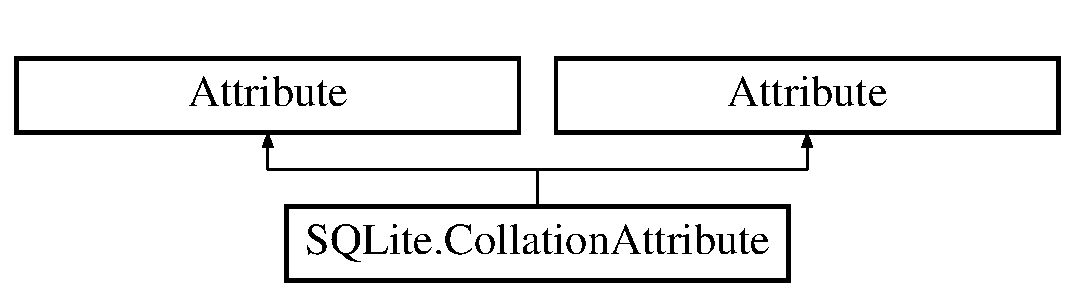
\includegraphics[height=2.000000cm]{classSQLite_1_1CollationAttribute}
\end{center}
\end{figure}
\subsection*{Public Member Functions}
\begin{DoxyCompactItemize}
\item 
\hypertarget{classSQLite_1_1CollationAttribute_a741b7b18adbbefa4c7922d254c8a3afc}{{\bfseries Collation\-Attribute} (string collation)}\label{classSQLite_1_1CollationAttribute_a741b7b18adbbefa4c7922d254c8a3afc}

\item 
\hypertarget{classSQLite_1_1CollationAttribute_a741b7b18adbbefa4c7922d254c8a3afc}{{\bfseries Collation\-Attribute} (string collation)}\label{classSQLite_1_1CollationAttribute_a741b7b18adbbefa4c7922d254c8a3afc}

\end{DoxyCompactItemize}
\subsection*{Properties}
\begin{DoxyCompactItemize}
\item 
\hypertarget{classSQLite_1_1CollationAttribute_a671ec768863418e52ff455d112063de2}{string {\bfseries Value}\hspace{0.3cm}{\ttfamily  \mbox{[}get, set\mbox{]}}}\label{classSQLite_1_1CollationAttribute_a671ec768863418e52ff455d112063de2}

\end{DoxyCompactItemize}


The documentation for this class was generated from the following file\-:\begin{DoxyCompactItemize}
\item 
packages/sqlite-\/net.\-1.\-0.\-8/content/S\-Q\-Lite.\-cs\end{DoxyCompactItemize}

\hypertarget{classclient_1_1Droid_1_1Resource_1_1Color}{\section{client.\-Droid.\-Resource.\-Color Class Reference}
\label{classclient_1_1Droid_1_1Resource_1_1Color}\index{client.\-Droid.\-Resource.\-Color@{client.\-Droid.\-Resource.\-Color}}
}
\subsection*{Public Attributes}
\begin{DoxyCompactItemize}
\item 
\hypertarget{classclient_1_1Droid_1_1Resource_1_1Color_abb05a40b34a7751b6d565bcada614f6c}{const int {\bfseries calendar\-\_\-active\-\_\-month\-\_\-bg} = 2131034112}\label{classclient_1_1Droid_1_1Resource_1_1Color_abb05a40b34a7751b6d565bcada614f6c}

\item 
\hypertarget{classclient_1_1Droid_1_1Resource_1_1Color_add1dca31d33f65edf8c781cfc18dda6f}{const int {\bfseries calendar\-\_\-bg} = 2131034113}\label{classclient_1_1Droid_1_1Resource_1_1Color_add1dca31d33f65edf8c781cfc18dda6f}

\item 
\hypertarget{classclient_1_1Droid_1_1Resource_1_1Color_a0f3f13f8233eb0cc8976a589af67fa06}{const int {\bfseries calendar\-\_\-divider} = 2131034114}\label{classclient_1_1Droid_1_1Resource_1_1Color_a0f3f13f8233eb0cc8976a589af67fa06}

\item 
\hypertarget{classclient_1_1Droid_1_1Resource_1_1Color_afa2c4f8a535b47f7a6681ef7c381a4b0}{const int {\bfseries calendar\-\_\-highlighted\-\_\-day\-\_\-bg} = 2131034117}\label{classclient_1_1Droid_1_1Resource_1_1Color_afa2c4f8a535b47f7a6681ef7c381a4b0}

\item 
\hypertarget{classclient_1_1Droid_1_1Resource_1_1Color_a643ff3a00bf9da24ba0048b3e4204f40}{const int {\bfseries calendar\-\_\-inactive\-\_\-month\-\_\-bg} = 2131034115}\label{classclient_1_1Droid_1_1Resource_1_1Color_a643ff3a00bf9da24ba0048b3e4204f40}

\item 
\hypertarget{classclient_1_1Droid_1_1Resource_1_1Color_a8b6d23df6f9cfc9310e5acd43e78e4d9}{const int {\bfseries calendar\-\_\-selected\-\_\-day\-\_\-bg} = 2131034116}\label{classclient_1_1Droid_1_1Resource_1_1Color_a8b6d23df6f9cfc9310e5acd43e78e4d9}

\item 
\hypertarget{classclient_1_1Droid_1_1Resource_1_1Color_a2d0a8be690db7bd467a77279c73404bd}{const int {\bfseries calendar\-\_\-selected\-\_\-range\-\_\-bg} = 2131034118}\label{classclient_1_1Droid_1_1Resource_1_1Color_a2d0a8be690db7bd467a77279c73404bd}

\item 
\hypertarget{classclient_1_1Droid_1_1Resource_1_1Color_ac2e368bc995e04cfb4cdea60826cdaa7}{const int {\bfseries calendar\-\_\-text\-\_\-active} = 2131034120}\label{classclient_1_1Droid_1_1Resource_1_1Color_ac2e368bc995e04cfb4cdea60826cdaa7}

\item 
\hypertarget{classclient_1_1Droid_1_1Resource_1_1Color_a96ad5f8118faf1e38e409a586e6621dd}{const int {\bfseries calendar\-\_\-text\-\_\-inactive} = 2131034119}\label{classclient_1_1Droid_1_1Resource_1_1Color_a96ad5f8118faf1e38e409a586e6621dd}

\item 
\hypertarget{classclient_1_1Droid_1_1Resource_1_1Color_a6bb63dbcd298e38f8b8bebda75a2ac84}{const int {\bfseries calendar\-\_\-text\-\_\-selected} = 2131034121}\label{classclient_1_1Droid_1_1Resource_1_1Color_a6bb63dbcd298e38f8b8bebda75a2ac84}

\item 
\hypertarget{classclient_1_1Droid_1_1Resource_1_1Color_ac39137bd5c7c8fa37b2328ac46afd509}{const int {\bfseries calendar\-\_\-text\-\_\-selector} = 2131034123}\label{classclient_1_1Droid_1_1Resource_1_1Color_ac39137bd5c7c8fa37b2328ac46afd509}

\item 
\hypertarget{classclient_1_1Droid_1_1Resource_1_1Color_a0bcd6582ca8e22231df6ba95f796a477}{const int {\bfseries calendar\-\_\-text\-\_\-unselectable} = 2131034122}\label{classclient_1_1Droid_1_1Resource_1_1Color_a0bcd6582ca8e22231df6ba95f796a477}

\end{DoxyCompactItemize}


The documentation for this class was generated from the following file\-:\begin{DoxyCompactItemize}
\item 
client/client/client.\-Android/\-Resources/Resource.\-designer.\-cs\end{DoxyCompactItemize}

\hypertarget{classSQLite_1_1TableMapping_1_1Column}{}\section{S\+Q\+Lite.\+Table\+Mapping.\+Column Class Reference}
\label{classSQLite_1_1TableMapping_1_1Column}\index{S\+Q\+Lite.\+Table\+Mapping.\+Column@{S\+Q\+Lite.\+Table\+Mapping.\+Column}}
\subsection*{Public Member Functions}
\begin{DoxyCompactItemize}
\item 
\hypertarget{classSQLite_1_1TableMapping_1_1Column_a404e36f92ab57bcc8f903a78dc47badf}{}{\bfseries Column} (Property\+Info prop, Create\+Flags create\+Flags=Create\+Flags.\+None)\label{classSQLite_1_1TableMapping_1_1Column_a404e36f92ab57bcc8f903a78dc47badf}

\item 
\hypertarget{classSQLite_1_1TableMapping_1_1Column_a0f57d48181580599bd9b4aa6db68687c}{}void {\bfseries Set\+Value} (object obj, object val)\label{classSQLite_1_1TableMapping_1_1Column_a0f57d48181580599bd9b4aa6db68687c}

\item 
\hypertarget{classSQLite_1_1TableMapping_1_1Column_ac2e9f8110d390d1fa630ebb0d345c293}{}object {\bfseries Get\+Value} (object obj)\label{classSQLite_1_1TableMapping_1_1Column_ac2e9f8110d390d1fa630ebb0d345c293}

\end{DoxyCompactItemize}
\subsection*{Properties}
\begin{DoxyCompactItemize}
\item 
\hypertarget{classSQLite_1_1TableMapping_1_1Column_a95c3ae2c8502cb3074751fbfee766bb0}{}string {\bfseries Name}\hspace{0.3cm}{\ttfamily  \mbox{[}get\mbox{]}}\label{classSQLite_1_1TableMapping_1_1Column_a95c3ae2c8502cb3074751fbfee766bb0}

\item 
\hypertarget{classSQLite_1_1TableMapping_1_1Column_af4b9a6b1eddbba6a9ec9dc2f9a8b6820}{}string {\bfseries Property\+Name}\hspace{0.3cm}{\ttfamily  \mbox{[}get\mbox{]}}\label{classSQLite_1_1TableMapping_1_1Column_af4b9a6b1eddbba6a9ec9dc2f9a8b6820}

\item 
\hypertarget{classSQLite_1_1TableMapping_1_1Column_afb3b922b5b0eb59eb826bb26b9838d61}{}Type {\bfseries Column\+Type}\hspace{0.3cm}{\ttfamily  \mbox{[}get\mbox{]}}\label{classSQLite_1_1TableMapping_1_1Column_afb3b922b5b0eb59eb826bb26b9838d61}

\item 
\hypertarget{classSQLite_1_1TableMapping_1_1Column_a6d8ba39bedd7336a17c5271479c7bb5a}{}string {\bfseries Collation}\hspace{0.3cm}{\ttfamily  \mbox{[}get\mbox{]}}\label{classSQLite_1_1TableMapping_1_1Column_a6d8ba39bedd7336a17c5271479c7bb5a}

\item 
\hypertarget{classSQLite_1_1TableMapping_1_1Column_a8cdcb1406f9ef7472b829f34c1f96360}{}bool {\bfseries Is\+Auto\+Inc}\hspace{0.3cm}{\ttfamily  \mbox{[}get\mbox{]}}\label{classSQLite_1_1TableMapping_1_1Column_a8cdcb1406f9ef7472b829f34c1f96360}

\item 
\hypertarget{classSQLite_1_1TableMapping_1_1Column_a5775c9a99e9b3ee8dd8f34b162b1e4ab}{}bool {\bfseries Is\+Auto\+Guid}\hspace{0.3cm}{\ttfamily  \mbox{[}get\mbox{]}}\label{classSQLite_1_1TableMapping_1_1Column_a5775c9a99e9b3ee8dd8f34b162b1e4ab}

\item 
\hypertarget{classSQLite_1_1TableMapping_1_1Column_a74b6f353e1632310fa12414e36407c50}{}bool {\bfseries Is\+P\+K}\hspace{0.3cm}{\ttfamily  \mbox{[}get\mbox{]}}\label{classSQLite_1_1TableMapping_1_1Column_a74b6f353e1632310fa12414e36407c50}

\item 
\hypertarget{classSQLite_1_1TableMapping_1_1Column_a5153b02c01f808c46d83f1bccc23aa40}{}I\+Enumerable$<$ \hyperlink{classSQLite_1_1IndexedAttribute}{Indexed\+Attribute} $>$ {\bfseries Indices}\hspace{0.3cm}{\ttfamily  \mbox{[}get, set\mbox{]}}\label{classSQLite_1_1TableMapping_1_1Column_a5153b02c01f808c46d83f1bccc23aa40}

\item 
\hypertarget{classSQLite_1_1TableMapping_1_1Column_a2ff8d12dcf449ca9407c4c3222521c96}{}bool {\bfseries Is\+Nullable}\hspace{0.3cm}{\ttfamily  \mbox{[}get\mbox{]}}\label{classSQLite_1_1TableMapping_1_1Column_a2ff8d12dcf449ca9407c4c3222521c96}

\item 
\hypertarget{classSQLite_1_1TableMapping_1_1Column_a762d97a3a799c0f7a31b034eb0f3db71}{}int {\bfseries Max\+String\+Length}\hspace{0.3cm}{\ttfamily  \mbox{[}get\mbox{]}}\label{classSQLite_1_1TableMapping_1_1Column_a762d97a3a799c0f7a31b034eb0f3db71}

\end{DoxyCompactItemize}


The documentation for this class was generated from the following file\+:\begin{DoxyCompactItemize}
\item 
packages/sqlite-\/net.\+1.\+0.\+8/content/S\+Q\+Lite.\+cs\end{DoxyCompactItemize}

\hypertarget{classSQLite_1_1ColumnAttribute}{}\section{S\+Q\+Lite.\+Column\+Attribute Class Reference}
\label{classSQLite_1_1ColumnAttribute}\index{S\+Q\+Lite.\+Column\+Attribute@{S\+Q\+Lite.\+Column\+Attribute}}
Inheritance diagram for S\+Q\+Lite.\+Column\+Attribute\+:\begin{figure}[H]
\begin{center}
\leavevmode
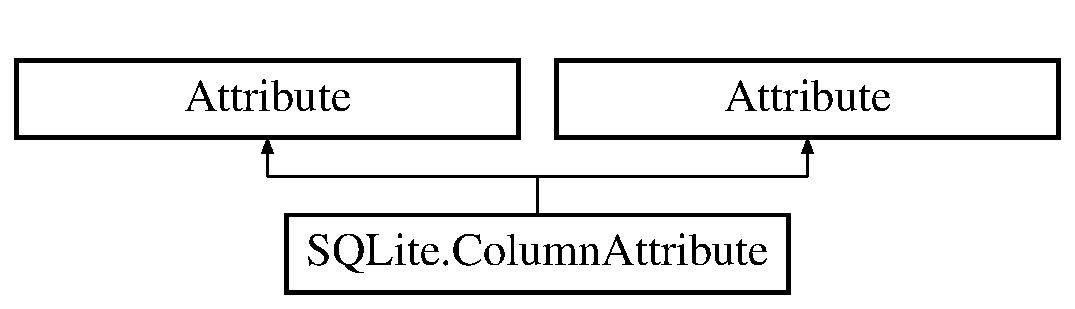
\includegraphics[height=2.000000cm]{classSQLite_1_1ColumnAttribute}
\end{center}
\end{figure}
\subsection*{Public Member Functions}
\begin{DoxyCompactItemize}
\item 
\hypertarget{classSQLite_1_1ColumnAttribute_aa7ecb3d322d1fde710f51558b314ad6f}{}{\bfseries Column\+Attribute} (string name)\label{classSQLite_1_1ColumnAttribute_aa7ecb3d322d1fde710f51558b314ad6f}

\end{DoxyCompactItemize}
\subsection*{Properties}
\begin{DoxyCompactItemize}
\item 
\hypertarget{classSQLite_1_1ColumnAttribute_af2e6c8ab9f0b1ce7f10ea75346f9b3c8}{}string {\bfseries Name}\hspace{0.3cm}{\ttfamily  \mbox{[}get, set\mbox{]}}\label{classSQLite_1_1ColumnAttribute_af2e6c8ab9f0b1ce7f10ea75346f9b3c8}

\end{DoxyCompactItemize}


The documentation for this class was generated from the following file\+:\begin{DoxyCompactItemize}
\item 
packages/sqlite-\/net.\+1.\+0.\+8/content/S\+Q\+Lite.\+cs\end{DoxyCompactItemize}

\hypertarget{classSQLite_1_1SQLiteConnection_1_1ColumnInfo}{\section{S\-Q\-Lite.\-S\-Q\-Lite\-Connection.\-Column\-Info Class Reference}
\label{classSQLite_1_1SQLiteConnection_1_1ColumnInfo}\index{S\-Q\-Lite.\-S\-Q\-Lite\-Connection.\-Column\-Info@{S\-Q\-Lite.\-S\-Q\-Lite\-Connection.\-Column\-Info}}
}
\subsection*{Public Member Functions}
\begin{DoxyCompactItemize}
\item 
\hypertarget{classSQLite_1_1SQLiteConnection_1_1ColumnInfo_af1ba3d13d1ccc9d2389c086f4e64610c}{override string {\bfseries To\-String} ()}\label{classSQLite_1_1SQLiteConnection_1_1ColumnInfo_af1ba3d13d1ccc9d2389c086f4e64610c}

\item 
\hypertarget{classSQLite_1_1SQLiteConnection_1_1ColumnInfo_af1ba3d13d1ccc9d2389c086f4e64610c}{override string {\bfseries To\-String} ()}\label{classSQLite_1_1SQLiteConnection_1_1ColumnInfo_af1ba3d13d1ccc9d2389c086f4e64610c}

\end{DoxyCompactItemize}
\subsection*{Properties}
\begin{DoxyCompactItemize}
\item 
\hypertarget{classSQLite_1_1SQLiteConnection_1_1ColumnInfo_abb54a8246c842238b86ae27252ed9590}{string {\bfseries Name}\hspace{0.3cm}{\ttfamily  \mbox{[}get, set\mbox{]}}}\label{classSQLite_1_1SQLiteConnection_1_1ColumnInfo_abb54a8246c842238b86ae27252ed9590}

\item 
\hypertarget{classSQLite_1_1SQLiteConnection_1_1ColumnInfo_a830462120a513cacefa6c59550e06fd5}{int {\bfseries notnull}\hspace{0.3cm}{\ttfamily  \mbox{[}get, set\mbox{]}}}\label{classSQLite_1_1SQLiteConnection_1_1ColumnInfo_a830462120a513cacefa6c59550e06fd5}

\end{DoxyCompactItemize}


The documentation for this class was generated from the following file\-:\begin{DoxyCompactItemize}
\item 
packages/sqlite-\/net.\-1.\-0.\-8/content/S\-Q\-Lite.\-cs\end{DoxyCompactItemize}

\hypertarget{classCore_1_1Models_1_1Constants}{}\section{Core.\+Models.\+Constants Class Reference}
\label{classCore_1_1Models_1_1Constants}\index{Core.\+Models.\+Constants@{Core.\+Models.\+Constants}}


all constants which should be known by the server and client  


\subsection*{Public Attributes}
\begin{DoxyCompactItemize}
\item 
const double \hyperlink{classCore_1_1Models_1_1Constants_adde91f87a25a57db171667f80b72d69f}{C\+E\+L\+L\+\_\+\+S\+I\+Z\+E} = 4
\begin{DoxyCompactList}\small\item\em size of a cell at the equator (in meters) \end{DoxyCompactList}\item 
const double \hyperlink{classCore_1_1Models_1_1Constants_ad31578c20b30dd96faf43b7a9f7b0389}{E\+A\+R\+T\+H\+\_\+\+C\+I\+R\+C\+U\+M\+F\+E\+R\+E\+N\+C\+E} = 40075036.\+0
\begin{DoxyCompactList}\small\item\em earth size at equator (in meters) \end{DoxyCompactList}\item 
const int \hyperlink{classCore_1_1Models_1_1Constants_a2d02174b6a70404c1d8093c81eb47cb2}{R\+E\+G\+I\+O\+N\+\_\+\+S\+I\+Z\+E\+\_\+\+X} = 32
\begin{DoxyCompactList}\small\item\em amount of cells per region x \end{DoxyCompactList}\item 
const int \hyperlink{classCore_1_1Models_1_1Constants_ad7f91cdefc9377eb37c98a50e0d1c068}{R\+E\+G\+I\+O\+N\+\_\+\+S\+I\+Z\+E\+\_\+\+Y} = 32
\begin{DoxyCompactList}\small\item\em amount of cells per region y \end{DoxyCompactList}\item 
const int \hyperlink{classCore_1_1Models_1_1Constants_a26b3d6b0c7f17fdac4b0789c3a6adec6}{M\+A\+J\+O\+R\+\_\+\+R\+E\+G\+I\+O\+N\+\_\+\+S\+I\+Z\+E\+\_\+\+X} = 16
\begin{DoxyCompactList}\small\item\em amount of regions per folder x \end{DoxyCompactList}\item 
const int \hyperlink{classCore_1_1Models_1_1Constants_ad49dbef4256b0be04e921acc8bcef4a8}{M\+A\+J\+O\+R\+\_\+\+R\+E\+G\+I\+O\+N\+\_\+\+S\+I\+Z\+E\+\_\+\+Y} = 16
\begin{DoxyCompactList}\small\item\em amount of regions per folder y \end{DoxyCompactList}\item 
const int \hyperlink{classCore_1_1Models_1_1Constants_a04216f06fce4df1266355ba32c59ac21}{S\+T\+A\+R\+T\+\_\+\+X} = 41504
\begin{DoxyCompactList}\small\item\em start x of playable world \end{DoxyCompactList}\item 
const int \hyperlink{classCore_1_1Models_1_1Constants_ab564a2138347d9c65862ffe4d80c6735}{E\+N\+D\+\_\+\+X} = 41519
\begin{DoxyCompactList}\small\item\em end x of playable world \end{DoxyCompactList}\item 
const int \hyperlink{classCore_1_1Models_1_1Constants_a0da8b0008fff8b2529d5a8e298b29e5f}{S\+T\+A\+R\+T\+\_\+\+Y} = 26184
\begin{DoxyCompactList}\small\item\em start y of playable world \end{DoxyCompactList}\item 
const int \hyperlink{classCore_1_1Models_1_1Constants_ae2cd96ff453731f63095739737f184b4}{E\+N\+D\+\_\+\+Y} = 26191
\begin{DoxyCompactList}\small\item\em end y of playable world \end{DoxyCompactList}\item 
const int \hyperlink{classCore_1_1Models_1_1Constants_a09b8f7514cdf1d440f7bbaff8fe843c2}{M\+A\+X\+\_\+\+E\+N\+T\+R\+I\+E\+S\+\_\+\+P\+E\+R\+\_\+\+C\+O\+N\+N\+E\+C\+T\+I\+O\+N} = 25
\begin{DoxyCompactList}\small\item\em if there are more than entries in a Linked\+List/array, the A\+P\+I will dismiss the request for safety reasons \end{DoxyCompactList}\item 
const int \hyperlink{classCore_1_1Models_1_1Constants_ae34c70369e0c6c6f34f5b5275625afdb}{R\+E\+G\+I\+O\+N\+\_\+\+L\+O\+C\+K\+\_\+\+W\+A\+I\+T\+\_\+\+T\+I\+M\+E} = 0
\begin{DoxyCompactList}\small\item\em wait time for region writer lock \end{DoxyCompactList}\item 
const int \hyperlink{classCore_1_1Models_1_1Constants_a3132eb59e27938a80a4ca4d047f4912f}{R\+A\+N\+G\+E\+\_\+\+I\+N\+\_\+\+M\+E\+E\+L\+E\+\_\+\+M\+A\+L\+U\+S} = 10
\begin{DoxyCompactList}\small\item\em The minus point for range units in melee combat. \end{DoxyCompactList}\item 
const int \hyperlink{classCore_1_1Models_1_1Constants_a3813d958b2e6df3057078b3569fdff4c}{H\+E\+A\+D\+Q\+U\+A\+R\+T\+E\+R\+\_\+\+T\+E\+R\+R\+I\+T\+O\+R\+Y\+\_\+\+R\+A\+N\+G\+E} = 4
\begin{DoxyCompactList}\small\item\em Get the range from the ownership radius for the headquarter. \end{DoxyCompactList}\item 
const int \hyperlink{classCore_1_1Models_1_1Constants_a64ce972b2af4cf4888944e71e9086dca}{G\+U\+A\+R\+D\+T\+O\+W\+E\+R\+\_\+\+T\+E\+R\+R\+I\+T\+O\+R\+Y\+\_\+\+R\+A\+N\+G\+E} = 2
\begin{DoxyCompactList}\small\item\em Get the range from the ownership radius for the guard tower. \end{DoxyCompactList}\item 
const int \hyperlink{classCore_1_1Models_1_1Constants_afab1e8f29a7e873783bc2c0aabaf4274}{H\+E\+A\+D\+Q\+U\+A\+R\+T\+E\+R\+\_\+\+S\+T\+O\+R\+A\+G\+E\+\_\+\+V\+A\+L\+U\+E} = 100
\begin{DoxyCompactList}\small\item\em The H\+Q storage value. \end{DoxyCompactList}\item 
const int \hyperlink{classCore_1_1Models_1_1Constants_aa59b895c1c117046c226c8864ee6e137}{P\+O\+P\+U\+L\+A\+T\+I\+O\+N\+\_\+\+S\+T\+O\+R\+A\+G\+E\+\_\+\+V\+A\+L\+U\+E} = 25
\begin{DoxyCompactList}\small\item\em The ground population storage. \end{DoxyCompactList}\item 
const int \hyperlink{classCore_1_1Models_1_1Constants_a7084aeeac217877ec00107e5a9b2356a}{S\+C\+R\+A\+P\+\_\+\+S\+T\+O\+R\+A\+G\+E\+\_\+\+V\+A\+L\+U\+E} = 50
\begin{DoxyCompactList}\small\item\em The ground scrap storage \end{DoxyCompactList}\item 
const int \hyperlink{classCore_1_1Models_1_1Constants_a73dd9150d21d41b1e61af6c163d8cb6c}{E\+N\+E\+R\+G\+Y\+\_\+\+M\+A\+X\+\_\+\+V\+A\+L\+U\+E} = 20
\begin{DoxyCompactList}\small\item\em The energy value. \end{DoxyCompactList}\item 
const int \hyperlink{classCore_1_1Models_1_1Constants_a1ab07bbbce0393349cffa44d47d306cd}{T\+E\+C\+H\+N\+O\+L\+O\+G\+Y\+\_\+\+M\+A\+X\+\_\+\+V\+A\+L\+U\+E} = 7
\begin{DoxyCompactList}\small\item\em The technology maximum value. \end{DoxyCompactList}\item 
const float \hyperlink{classCore_1_1Models_1_1Constants_a2a4a1624387cb4495c03b99ef7e3086a}{T\+E\+C\+H\+N\+O\+L\+O\+G\+Y\+\_\+\+I\+N\+C\+R\+E\+M\+E\+N\+T\+\_\+\+V\+A\+L\+U\+E} = 0.\+1f
\begin{DoxyCompactList}\small\item\em The increment value for technology resource. \end{DoxyCompactList}\item 
const int \hyperlink{classCore_1_1Models_1_1Constants_a455082f6f12f13a8c7d4f742f9a7a7b0}{S\+C\+R\+A\+P\+\_\+\+I\+N\+C\+R\+E\+M\+E\+N\+T\+\_\+\+V\+A\+L\+U\+E} = 2
\begin{DoxyCompactList}\small\item\em The increment value for scrap resource. \end{DoxyCompactList}\item 
const float \hyperlink{classCore_1_1Models_1_1Constants_ad71a4c6614e19c0ae08b56caa5241750}{P\+L\+U\+T\+O\+N\+I\+U\+M\+\_\+\+I\+N\+C\+R\+E\+M\+E\+N\+T\+\_\+\+V\+A\+L\+U\+E} = 0.\+3f
\begin{DoxyCompactList}\small\item\em The increment value for plutonium resource. \end{DoxyCompactList}\end{DoxyCompactItemize}


\subsection{Detailed Description}
all constants which should be known by the server and client 



\subsection{Member Data Documentation}
\hypertarget{classCore_1_1Models_1_1Constants_adde91f87a25a57db171667f80b72d69f}{}\index{Core\+::\+Models\+::\+Constants@{Core\+::\+Models\+::\+Constants}!C\+E\+L\+L\+\_\+\+S\+I\+Z\+E@{C\+E\+L\+L\+\_\+\+S\+I\+Z\+E}}
\index{C\+E\+L\+L\+\_\+\+S\+I\+Z\+E@{C\+E\+L\+L\+\_\+\+S\+I\+Z\+E}!Core\+::\+Models\+::\+Constants@{Core\+::\+Models\+::\+Constants}}
\subsubsection[{C\+E\+L\+L\+\_\+\+S\+I\+Z\+E}]{\setlength{\rightskip}{0pt plus 5cm}const double Core.\+Models.\+Constants.\+C\+E\+L\+L\+\_\+\+S\+I\+Z\+E = 4}\label{classCore_1_1Models_1_1Constants_adde91f87a25a57db171667f80b72d69f}


size of a cell at the equator (in meters) 

\hypertarget{classCore_1_1Models_1_1Constants_ad31578c20b30dd96faf43b7a9f7b0389}{}\index{Core\+::\+Models\+::\+Constants@{Core\+::\+Models\+::\+Constants}!E\+A\+R\+T\+H\+\_\+\+C\+I\+R\+C\+U\+M\+F\+E\+R\+E\+N\+C\+E@{E\+A\+R\+T\+H\+\_\+\+C\+I\+R\+C\+U\+M\+F\+E\+R\+E\+N\+C\+E}}
\index{E\+A\+R\+T\+H\+\_\+\+C\+I\+R\+C\+U\+M\+F\+E\+R\+E\+N\+C\+E@{E\+A\+R\+T\+H\+\_\+\+C\+I\+R\+C\+U\+M\+F\+E\+R\+E\+N\+C\+E}!Core\+::\+Models\+::\+Constants@{Core\+::\+Models\+::\+Constants}}
\subsubsection[{E\+A\+R\+T\+H\+\_\+\+C\+I\+R\+C\+U\+M\+F\+E\+R\+E\+N\+C\+E}]{\setlength{\rightskip}{0pt plus 5cm}const double Core.\+Models.\+Constants.\+E\+A\+R\+T\+H\+\_\+\+C\+I\+R\+C\+U\+M\+F\+E\+R\+E\+N\+C\+E = 40075036.\+0}\label{classCore_1_1Models_1_1Constants_ad31578c20b30dd96faf43b7a9f7b0389}


earth size at equator (in meters) 

\hypertarget{classCore_1_1Models_1_1Constants_ab564a2138347d9c65862ffe4d80c6735}{}\index{Core\+::\+Models\+::\+Constants@{Core\+::\+Models\+::\+Constants}!E\+N\+D\+\_\+\+X@{E\+N\+D\+\_\+\+X}}
\index{E\+N\+D\+\_\+\+X@{E\+N\+D\+\_\+\+X}!Core\+::\+Models\+::\+Constants@{Core\+::\+Models\+::\+Constants}}
\subsubsection[{E\+N\+D\+\_\+\+X}]{\setlength{\rightskip}{0pt plus 5cm}const int Core.\+Models.\+Constants.\+E\+N\+D\+\_\+\+X = 41519}\label{classCore_1_1Models_1_1Constants_ab564a2138347d9c65862ffe4d80c6735}


end x of playable world 

\hypertarget{classCore_1_1Models_1_1Constants_ae2cd96ff453731f63095739737f184b4}{}\index{Core\+::\+Models\+::\+Constants@{Core\+::\+Models\+::\+Constants}!E\+N\+D\+\_\+\+Y@{E\+N\+D\+\_\+\+Y}}
\index{E\+N\+D\+\_\+\+Y@{E\+N\+D\+\_\+\+Y}!Core\+::\+Models\+::\+Constants@{Core\+::\+Models\+::\+Constants}}
\subsubsection[{E\+N\+D\+\_\+\+Y}]{\setlength{\rightskip}{0pt plus 5cm}const int Core.\+Models.\+Constants.\+E\+N\+D\+\_\+\+Y = 26191}\label{classCore_1_1Models_1_1Constants_ae2cd96ff453731f63095739737f184b4}


end y of playable world 

\hypertarget{classCore_1_1Models_1_1Constants_a73dd9150d21d41b1e61af6c163d8cb6c}{}\index{Core\+::\+Models\+::\+Constants@{Core\+::\+Models\+::\+Constants}!E\+N\+E\+R\+G\+Y\+\_\+\+M\+A\+X\+\_\+\+V\+A\+L\+U\+E@{E\+N\+E\+R\+G\+Y\+\_\+\+M\+A\+X\+\_\+\+V\+A\+L\+U\+E}}
\index{E\+N\+E\+R\+G\+Y\+\_\+\+M\+A\+X\+\_\+\+V\+A\+L\+U\+E@{E\+N\+E\+R\+G\+Y\+\_\+\+M\+A\+X\+\_\+\+V\+A\+L\+U\+E}!Core\+::\+Models\+::\+Constants@{Core\+::\+Models\+::\+Constants}}
\subsubsection[{E\+N\+E\+R\+G\+Y\+\_\+\+M\+A\+X\+\_\+\+V\+A\+L\+U\+E}]{\setlength{\rightskip}{0pt plus 5cm}const int Core.\+Models.\+Constants.\+E\+N\+E\+R\+G\+Y\+\_\+\+M\+A\+X\+\_\+\+V\+A\+L\+U\+E = 20}\label{classCore_1_1Models_1_1Constants_a73dd9150d21d41b1e61af6c163d8cb6c}


The energy value. 

\hypertarget{classCore_1_1Models_1_1Constants_a64ce972b2af4cf4888944e71e9086dca}{}\index{Core\+::\+Models\+::\+Constants@{Core\+::\+Models\+::\+Constants}!G\+U\+A\+R\+D\+T\+O\+W\+E\+R\+\_\+\+T\+E\+R\+R\+I\+T\+O\+R\+Y\+\_\+\+R\+A\+N\+G\+E@{G\+U\+A\+R\+D\+T\+O\+W\+E\+R\+\_\+\+T\+E\+R\+R\+I\+T\+O\+R\+Y\+\_\+\+R\+A\+N\+G\+E}}
\index{G\+U\+A\+R\+D\+T\+O\+W\+E\+R\+\_\+\+T\+E\+R\+R\+I\+T\+O\+R\+Y\+\_\+\+R\+A\+N\+G\+E@{G\+U\+A\+R\+D\+T\+O\+W\+E\+R\+\_\+\+T\+E\+R\+R\+I\+T\+O\+R\+Y\+\_\+\+R\+A\+N\+G\+E}!Core\+::\+Models\+::\+Constants@{Core\+::\+Models\+::\+Constants}}
\subsubsection[{G\+U\+A\+R\+D\+T\+O\+W\+E\+R\+\_\+\+T\+E\+R\+R\+I\+T\+O\+R\+Y\+\_\+\+R\+A\+N\+G\+E}]{\setlength{\rightskip}{0pt plus 5cm}const int Core.\+Models.\+Constants.\+G\+U\+A\+R\+D\+T\+O\+W\+E\+R\+\_\+\+T\+E\+R\+R\+I\+T\+O\+R\+Y\+\_\+\+R\+A\+N\+G\+E = 2}\label{classCore_1_1Models_1_1Constants_a64ce972b2af4cf4888944e71e9086dca}


Get the range from the ownership radius for the guard tower. 

\hypertarget{classCore_1_1Models_1_1Constants_afab1e8f29a7e873783bc2c0aabaf4274}{}\index{Core\+::\+Models\+::\+Constants@{Core\+::\+Models\+::\+Constants}!H\+E\+A\+D\+Q\+U\+A\+R\+T\+E\+R\+\_\+\+S\+T\+O\+R\+A\+G\+E\+\_\+\+V\+A\+L\+U\+E@{H\+E\+A\+D\+Q\+U\+A\+R\+T\+E\+R\+\_\+\+S\+T\+O\+R\+A\+G\+E\+\_\+\+V\+A\+L\+U\+E}}
\index{H\+E\+A\+D\+Q\+U\+A\+R\+T\+E\+R\+\_\+\+S\+T\+O\+R\+A\+G\+E\+\_\+\+V\+A\+L\+U\+E@{H\+E\+A\+D\+Q\+U\+A\+R\+T\+E\+R\+\_\+\+S\+T\+O\+R\+A\+G\+E\+\_\+\+V\+A\+L\+U\+E}!Core\+::\+Models\+::\+Constants@{Core\+::\+Models\+::\+Constants}}
\subsubsection[{H\+E\+A\+D\+Q\+U\+A\+R\+T\+E\+R\+\_\+\+S\+T\+O\+R\+A\+G\+E\+\_\+\+V\+A\+L\+U\+E}]{\setlength{\rightskip}{0pt plus 5cm}const int Core.\+Models.\+Constants.\+H\+E\+A\+D\+Q\+U\+A\+R\+T\+E\+R\+\_\+\+S\+T\+O\+R\+A\+G\+E\+\_\+\+V\+A\+L\+U\+E = 100}\label{classCore_1_1Models_1_1Constants_afab1e8f29a7e873783bc2c0aabaf4274}


The H\+Q storage value. 

\hypertarget{classCore_1_1Models_1_1Constants_a3813d958b2e6df3057078b3569fdff4c}{}\index{Core\+::\+Models\+::\+Constants@{Core\+::\+Models\+::\+Constants}!H\+E\+A\+D\+Q\+U\+A\+R\+T\+E\+R\+\_\+\+T\+E\+R\+R\+I\+T\+O\+R\+Y\+\_\+\+R\+A\+N\+G\+E@{H\+E\+A\+D\+Q\+U\+A\+R\+T\+E\+R\+\_\+\+T\+E\+R\+R\+I\+T\+O\+R\+Y\+\_\+\+R\+A\+N\+G\+E}}
\index{H\+E\+A\+D\+Q\+U\+A\+R\+T\+E\+R\+\_\+\+T\+E\+R\+R\+I\+T\+O\+R\+Y\+\_\+\+R\+A\+N\+G\+E@{H\+E\+A\+D\+Q\+U\+A\+R\+T\+E\+R\+\_\+\+T\+E\+R\+R\+I\+T\+O\+R\+Y\+\_\+\+R\+A\+N\+G\+E}!Core\+::\+Models\+::\+Constants@{Core\+::\+Models\+::\+Constants}}
\subsubsection[{H\+E\+A\+D\+Q\+U\+A\+R\+T\+E\+R\+\_\+\+T\+E\+R\+R\+I\+T\+O\+R\+Y\+\_\+\+R\+A\+N\+G\+E}]{\setlength{\rightskip}{0pt plus 5cm}const int Core.\+Models.\+Constants.\+H\+E\+A\+D\+Q\+U\+A\+R\+T\+E\+R\+\_\+\+T\+E\+R\+R\+I\+T\+O\+R\+Y\+\_\+\+R\+A\+N\+G\+E = 4}\label{classCore_1_1Models_1_1Constants_a3813d958b2e6df3057078b3569fdff4c}


Get the range from the ownership radius for the headquarter. 

\hypertarget{classCore_1_1Models_1_1Constants_a26b3d6b0c7f17fdac4b0789c3a6adec6}{}\index{Core\+::\+Models\+::\+Constants@{Core\+::\+Models\+::\+Constants}!M\+A\+J\+O\+R\+\_\+\+R\+E\+G\+I\+O\+N\+\_\+\+S\+I\+Z\+E\+\_\+\+X@{M\+A\+J\+O\+R\+\_\+\+R\+E\+G\+I\+O\+N\+\_\+\+S\+I\+Z\+E\+\_\+\+X}}
\index{M\+A\+J\+O\+R\+\_\+\+R\+E\+G\+I\+O\+N\+\_\+\+S\+I\+Z\+E\+\_\+\+X@{M\+A\+J\+O\+R\+\_\+\+R\+E\+G\+I\+O\+N\+\_\+\+S\+I\+Z\+E\+\_\+\+X}!Core\+::\+Models\+::\+Constants@{Core\+::\+Models\+::\+Constants}}
\subsubsection[{M\+A\+J\+O\+R\+\_\+\+R\+E\+G\+I\+O\+N\+\_\+\+S\+I\+Z\+E\+\_\+\+X}]{\setlength{\rightskip}{0pt plus 5cm}const int Core.\+Models.\+Constants.\+M\+A\+J\+O\+R\+\_\+\+R\+E\+G\+I\+O\+N\+\_\+\+S\+I\+Z\+E\+\_\+\+X = 16}\label{classCore_1_1Models_1_1Constants_a26b3d6b0c7f17fdac4b0789c3a6adec6}


amount of regions per folder x 

\hypertarget{classCore_1_1Models_1_1Constants_ad49dbef4256b0be04e921acc8bcef4a8}{}\index{Core\+::\+Models\+::\+Constants@{Core\+::\+Models\+::\+Constants}!M\+A\+J\+O\+R\+\_\+\+R\+E\+G\+I\+O\+N\+\_\+\+S\+I\+Z\+E\+\_\+\+Y@{M\+A\+J\+O\+R\+\_\+\+R\+E\+G\+I\+O\+N\+\_\+\+S\+I\+Z\+E\+\_\+\+Y}}
\index{M\+A\+J\+O\+R\+\_\+\+R\+E\+G\+I\+O\+N\+\_\+\+S\+I\+Z\+E\+\_\+\+Y@{M\+A\+J\+O\+R\+\_\+\+R\+E\+G\+I\+O\+N\+\_\+\+S\+I\+Z\+E\+\_\+\+Y}!Core\+::\+Models\+::\+Constants@{Core\+::\+Models\+::\+Constants}}
\subsubsection[{M\+A\+J\+O\+R\+\_\+\+R\+E\+G\+I\+O\+N\+\_\+\+S\+I\+Z\+E\+\_\+\+Y}]{\setlength{\rightskip}{0pt plus 5cm}const int Core.\+Models.\+Constants.\+M\+A\+J\+O\+R\+\_\+\+R\+E\+G\+I\+O\+N\+\_\+\+S\+I\+Z\+E\+\_\+\+Y = 16}\label{classCore_1_1Models_1_1Constants_ad49dbef4256b0be04e921acc8bcef4a8}


amount of regions per folder y 

\hypertarget{classCore_1_1Models_1_1Constants_a09b8f7514cdf1d440f7bbaff8fe843c2}{}\index{Core\+::\+Models\+::\+Constants@{Core\+::\+Models\+::\+Constants}!M\+A\+X\+\_\+\+E\+N\+T\+R\+I\+E\+S\+\_\+\+P\+E\+R\+\_\+\+C\+O\+N\+N\+E\+C\+T\+I\+O\+N@{M\+A\+X\+\_\+\+E\+N\+T\+R\+I\+E\+S\+\_\+\+P\+E\+R\+\_\+\+C\+O\+N\+N\+E\+C\+T\+I\+O\+N}}
\index{M\+A\+X\+\_\+\+E\+N\+T\+R\+I\+E\+S\+\_\+\+P\+E\+R\+\_\+\+C\+O\+N\+N\+E\+C\+T\+I\+O\+N@{M\+A\+X\+\_\+\+E\+N\+T\+R\+I\+E\+S\+\_\+\+P\+E\+R\+\_\+\+C\+O\+N\+N\+E\+C\+T\+I\+O\+N}!Core\+::\+Models\+::\+Constants@{Core\+::\+Models\+::\+Constants}}
\subsubsection[{M\+A\+X\+\_\+\+E\+N\+T\+R\+I\+E\+S\+\_\+\+P\+E\+R\+\_\+\+C\+O\+N\+N\+E\+C\+T\+I\+O\+N}]{\setlength{\rightskip}{0pt plus 5cm}const int Core.\+Models.\+Constants.\+M\+A\+X\+\_\+\+E\+N\+T\+R\+I\+E\+S\+\_\+\+P\+E\+R\+\_\+\+C\+O\+N\+N\+E\+C\+T\+I\+O\+N = 25}\label{classCore_1_1Models_1_1Constants_a09b8f7514cdf1d440f7bbaff8fe843c2}


if there are more than entries in a Linked\+List/array, the A\+P\+I will dismiss the request for safety reasons 

\hypertarget{classCore_1_1Models_1_1Constants_ad71a4c6614e19c0ae08b56caa5241750}{}\index{Core\+::\+Models\+::\+Constants@{Core\+::\+Models\+::\+Constants}!P\+L\+U\+T\+O\+N\+I\+U\+M\+\_\+\+I\+N\+C\+R\+E\+M\+E\+N\+T\+\_\+\+V\+A\+L\+U\+E@{P\+L\+U\+T\+O\+N\+I\+U\+M\+\_\+\+I\+N\+C\+R\+E\+M\+E\+N\+T\+\_\+\+V\+A\+L\+U\+E}}
\index{P\+L\+U\+T\+O\+N\+I\+U\+M\+\_\+\+I\+N\+C\+R\+E\+M\+E\+N\+T\+\_\+\+V\+A\+L\+U\+E@{P\+L\+U\+T\+O\+N\+I\+U\+M\+\_\+\+I\+N\+C\+R\+E\+M\+E\+N\+T\+\_\+\+V\+A\+L\+U\+E}!Core\+::\+Models\+::\+Constants@{Core\+::\+Models\+::\+Constants}}
\subsubsection[{P\+L\+U\+T\+O\+N\+I\+U\+M\+\_\+\+I\+N\+C\+R\+E\+M\+E\+N\+T\+\_\+\+V\+A\+L\+U\+E}]{\setlength{\rightskip}{0pt plus 5cm}const float Core.\+Models.\+Constants.\+P\+L\+U\+T\+O\+N\+I\+U\+M\+\_\+\+I\+N\+C\+R\+E\+M\+E\+N\+T\+\_\+\+V\+A\+L\+U\+E = 0.\+3f}\label{classCore_1_1Models_1_1Constants_ad71a4c6614e19c0ae08b56caa5241750}


The increment value for plutonium resource. 

\hypertarget{classCore_1_1Models_1_1Constants_aa59b895c1c117046c226c8864ee6e137}{}\index{Core\+::\+Models\+::\+Constants@{Core\+::\+Models\+::\+Constants}!P\+O\+P\+U\+L\+A\+T\+I\+O\+N\+\_\+\+S\+T\+O\+R\+A\+G\+E\+\_\+\+V\+A\+L\+U\+E@{P\+O\+P\+U\+L\+A\+T\+I\+O\+N\+\_\+\+S\+T\+O\+R\+A\+G\+E\+\_\+\+V\+A\+L\+U\+E}}
\index{P\+O\+P\+U\+L\+A\+T\+I\+O\+N\+\_\+\+S\+T\+O\+R\+A\+G\+E\+\_\+\+V\+A\+L\+U\+E@{P\+O\+P\+U\+L\+A\+T\+I\+O\+N\+\_\+\+S\+T\+O\+R\+A\+G\+E\+\_\+\+V\+A\+L\+U\+E}!Core\+::\+Models\+::\+Constants@{Core\+::\+Models\+::\+Constants}}
\subsubsection[{P\+O\+P\+U\+L\+A\+T\+I\+O\+N\+\_\+\+S\+T\+O\+R\+A\+G\+E\+\_\+\+V\+A\+L\+U\+E}]{\setlength{\rightskip}{0pt plus 5cm}const int Core.\+Models.\+Constants.\+P\+O\+P\+U\+L\+A\+T\+I\+O\+N\+\_\+\+S\+T\+O\+R\+A\+G\+E\+\_\+\+V\+A\+L\+U\+E = 25}\label{classCore_1_1Models_1_1Constants_aa59b895c1c117046c226c8864ee6e137}


The ground population storage. 

\hypertarget{classCore_1_1Models_1_1Constants_a3132eb59e27938a80a4ca4d047f4912f}{}\index{Core\+::\+Models\+::\+Constants@{Core\+::\+Models\+::\+Constants}!R\+A\+N\+G\+E\+\_\+\+I\+N\+\_\+\+M\+E\+E\+L\+E\+\_\+\+M\+A\+L\+U\+S@{R\+A\+N\+G\+E\+\_\+\+I\+N\+\_\+\+M\+E\+E\+L\+E\+\_\+\+M\+A\+L\+U\+S}}
\index{R\+A\+N\+G\+E\+\_\+\+I\+N\+\_\+\+M\+E\+E\+L\+E\+\_\+\+M\+A\+L\+U\+S@{R\+A\+N\+G\+E\+\_\+\+I\+N\+\_\+\+M\+E\+E\+L\+E\+\_\+\+M\+A\+L\+U\+S}!Core\+::\+Models\+::\+Constants@{Core\+::\+Models\+::\+Constants}}
\subsubsection[{R\+A\+N\+G\+E\+\_\+\+I\+N\+\_\+\+M\+E\+E\+L\+E\+\_\+\+M\+A\+L\+U\+S}]{\setlength{\rightskip}{0pt plus 5cm}const int Core.\+Models.\+Constants.\+R\+A\+N\+G\+E\+\_\+\+I\+N\+\_\+\+M\+E\+E\+L\+E\+\_\+\+M\+A\+L\+U\+S = 10}\label{classCore_1_1Models_1_1Constants_a3132eb59e27938a80a4ca4d047f4912f}


The minus point for range units in melee combat. 

\hypertarget{classCore_1_1Models_1_1Constants_ae34c70369e0c6c6f34f5b5275625afdb}{}\index{Core\+::\+Models\+::\+Constants@{Core\+::\+Models\+::\+Constants}!R\+E\+G\+I\+O\+N\+\_\+\+L\+O\+C\+K\+\_\+\+W\+A\+I\+T\+\_\+\+T\+I\+M\+E@{R\+E\+G\+I\+O\+N\+\_\+\+L\+O\+C\+K\+\_\+\+W\+A\+I\+T\+\_\+\+T\+I\+M\+E}}
\index{R\+E\+G\+I\+O\+N\+\_\+\+L\+O\+C\+K\+\_\+\+W\+A\+I\+T\+\_\+\+T\+I\+M\+E@{R\+E\+G\+I\+O\+N\+\_\+\+L\+O\+C\+K\+\_\+\+W\+A\+I\+T\+\_\+\+T\+I\+M\+E}!Core\+::\+Models\+::\+Constants@{Core\+::\+Models\+::\+Constants}}
\subsubsection[{R\+E\+G\+I\+O\+N\+\_\+\+L\+O\+C\+K\+\_\+\+W\+A\+I\+T\+\_\+\+T\+I\+M\+E}]{\setlength{\rightskip}{0pt plus 5cm}const int Core.\+Models.\+Constants.\+R\+E\+G\+I\+O\+N\+\_\+\+L\+O\+C\+K\+\_\+\+W\+A\+I\+T\+\_\+\+T\+I\+M\+E = 0}\label{classCore_1_1Models_1_1Constants_ae34c70369e0c6c6f34f5b5275625afdb}


wait time for region writer lock 

\hypertarget{classCore_1_1Models_1_1Constants_a2d02174b6a70404c1d8093c81eb47cb2}{}\index{Core\+::\+Models\+::\+Constants@{Core\+::\+Models\+::\+Constants}!R\+E\+G\+I\+O\+N\+\_\+\+S\+I\+Z\+E\+\_\+\+X@{R\+E\+G\+I\+O\+N\+\_\+\+S\+I\+Z\+E\+\_\+\+X}}
\index{R\+E\+G\+I\+O\+N\+\_\+\+S\+I\+Z\+E\+\_\+\+X@{R\+E\+G\+I\+O\+N\+\_\+\+S\+I\+Z\+E\+\_\+\+X}!Core\+::\+Models\+::\+Constants@{Core\+::\+Models\+::\+Constants}}
\subsubsection[{R\+E\+G\+I\+O\+N\+\_\+\+S\+I\+Z\+E\+\_\+\+X}]{\setlength{\rightskip}{0pt plus 5cm}const int Core.\+Models.\+Constants.\+R\+E\+G\+I\+O\+N\+\_\+\+S\+I\+Z\+E\+\_\+\+X = 32}\label{classCore_1_1Models_1_1Constants_a2d02174b6a70404c1d8093c81eb47cb2}


amount of cells per region x 

\hypertarget{classCore_1_1Models_1_1Constants_ad7f91cdefc9377eb37c98a50e0d1c068}{}\index{Core\+::\+Models\+::\+Constants@{Core\+::\+Models\+::\+Constants}!R\+E\+G\+I\+O\+N\+\_\+\+S\+I\+Z\+E\+\_\+\+Y@{R\+E\+G\+I\+O\+N\+\_\+\+S\+I\+Z\+E\+\_\+\+Y}}
\index{R\+E\+G\+I\+O\+N\+\_\+\+S\+I\+Z\+E\+\_\+\+Y@{R\+E\+G\+I\+O\+N\+\_\+\+S\+I\+Z\+E\+\_\+\+Y}!Core\+::\+Models\+::\+Constants@{Core\+::\+Models\+::\+Constants}}
\subsubsection[{R\+E\+G\+I\+O\+N\+\_\+\+S\+I\+Z\+E\+\_\+\+Y}]{\setlength{\rightskip}{0pt plus 5cm}const int Core.\+Models.\+Constants.\+R\+E\+G\+I\+O\+N\+\_\+\+S\+I\+Z\+E\+\_\+\+Y = 32}\label{classCore_1_1Models_1_1Constants_ad7f91cdefc9377eb37c98a50e0d1c068}


amount of cells per region y 

\hypertarget{classCore_1_1Models_1_1Constants_a455082f6f12f13a8c7d4f742f9a7a7b0}{}\index{Core\+::\+Models\+::\+Constants@{Core\+::\+Models\+::\+Constants}!S\+C\+R\+A\+P\+\_\+\+I\+N\+C\+R\+E\+M\+E\+N\+T\+\_\+\+V\+A\+L\+U\+E@{S\+C\+R\+A\+P\+\_\+\+I\+N\+C\+R\+E\+M\+E\+N\+T\+\_\+\+V\+A\+L\+U\+E}}
\index{S\+C\+R\+A\+P\+\_\+\+I\+N\+C\+R\+E\+M\+E\+N\+T\+\_\+\+V\+A\+L\+U\+E@{S\+C\+R\+A\+P\+\_\+\+I\+N\+C\+R\+E\+M\+E\+N\+T\+\_\+\+V\+A\+L\+U\+E}!Core\+::\+Models\+::\+Constants@{Core\+::\+Models\+::\+Constants}}
\subsubsection[{S\+C\+R\+A\+P\+\_\+\+I\+N\+C\+R\+E\+M\+E\+N\+T\+\_\+\+V\+A\+L\+U\+E}]{\setlength{\rightskip}{0pt plus 5cm}const int Core.\+Models.\+Constants.\+S\+C\+R\+A\+P\+\_\+\+I\+N\+C\+R\+E\+M\+E\+N\+T\+\_\+\+V\+A\+L\+U\+E = 2}\label{classCore_1_1Models_1_1Constants_a455082f6f12f13a8c7d4f742f9a7a7b0}


The increment value for scrap resource. 

\hypertarget{classCore_1_1Models_1_1Constants_a7084aeeac217877ec00107e5a9b2356a}{}\index{Core\+::\+Models\+::\+Constants@{Core\+::\+Models\+::\+Constants}!S\+C\+R\+A\+P\+\_\+\+S\+T\+O\+R\+A\+G\+E\+\_\+\+V\+A\+L\+U\+E@{S\+C\+R\+A\+P\+\_\+\+S\+T\+O\+R\+A\+G\+E\+\_\+\+V\+A\+L\+U\+E}}
\index{S\+C\+R\+A\+P\+\_\+\+S\+T\+O\+R\+A\+G\+E\+\_\+\+V\+A\+L\+U\+E@{S\+C\+R\+A\+P\+\_\+\+S\+T\+O\+R\+A\+G\+E\+\_\+\+V\+A\+L\+U\+E}!Core\+::\+Models\+::\+Constants@{Core\+::\+Models\+::\+Constants}}
\subsubsection[{S\+C\+R\+A\+P\+\_\+\+S\+T\+O\+R\+A\+G\+E\+\_\+\+V\+A\+L\+U\+E}]{\setlength{\rightskip}{0pt plus 5cm}const int Core.\+Models.\+Constants.\+S\+C\+R\+A\+P\+\_\+\+S\+T\+O\+R\+A\+G\+E\+\_\+\+V\+A\+L\+U\+E = 50}\label{classCore_1_1Models_1_1Constants_a7084aeeac217877ec00107e5a9b2356a}


The ground scrap storage 

\hypertarget{classCore_1_1Models_1_1Constants_a04216f06fce4df1266355ba32c59ac21}{}\index{Core\+::\+Models\+::\+Constants@{Core\+::\+Models\+::\+Constants}!S\+T\+A\+R\+T\+\_\+\+X@{S\+T\+A\+R\+T\+\_\+\+X}}
\index{S\+T\+A\+R\+T\+\_\+\+X@{S\+T\+A\+R\+T\+\_\+\+X}!Core\+::\+Models\+::\+Constants@{Core\+::\+Models\+::\+Constants}}
\subsubsection[{S\+T\+A\+R\+T\+\_\+\+X}]{\setlength{\rightskip}{0pt plus 5cm}const int Core.\+Models.\+Constants.\+S\+T\+A\+R\+T\+\_\+\+X = 41504}\label{classCore_1_1Models_1_1Constants_a04216f06fce4df1266355ba32c59ac21}


start x of playable world 

\hypertarget{classCore_1_1Models_1_1Constants_a0da8b0008fff8b2529d5a8e298b29e5f}{}\index{Core\+::\+Models\+::\+Constants@{Core\+::\+Models\+::\+Constants}!S\+T\+A\+R\+T\+\_\+\+Y@{S\+T\+A\+R\+T\+\_\+\+Y}}
\index{S\+T\+A\+R\+T\+\_\+\+Y@{S\+T\+A\+R\+T\+\_\+\+Y}!Core\+::\+Models\+::\+Constants@{Core\+::\+Models\+::\+Constants}}
\subsubsection[{S\+T\+A\+R\+T\+\_\+\+Y}]{\setlength{\rightskip}{0pt plus 5cm}const int Core.\+Models.\+Constants.\+S\+T\+A\+R\+T\+\_\+\+Y = 26184}\label{classCore_1_1Models_1_1Constants_a0da8b0008fff8b2529d5a8e298b29e5f}


start y of playable world 

\hypertarget{classCore_1_1Models_1_1Constants_a2a4a1624387cb4495c03b99ef7e3086a}{}\index{Core\+::\+Models\+::\+Constants@{Core\+::\+Models\+::\+Constants}!T\+E\+C\+H\+N\+O\+L\+O\+G\+Y\+\_\+\+I\+N\+C\+R\+E\+M\+E\+N\+T\+\_\+\+V\+A\+L\+U\+E@{T\+E\+C\+H\+N\+O\+L\+O\+G\+Y\+\_\+\+I\+N\+C\+R\+E\+M\+E\+N\+T\+\_\+\+V\+A\+L\+U\+E}}
\index{T\+E\+C\+H\+N\+O\+L\+O\+G\+Y\+\_\+\+I\+N\+C\+R\+E\+M\+E\+N\+T\+\_\+\+V\+A\+L\+U\+E@{T\+E\+C\+H\+N\+O\+L\+O\+G\+Y\+\_\+\+I\+N\+C\+R\+E\+M\+E\+N\+T\+\_\+\+V\+A\+L\+U\+E}!Core\+::\+Models\+::\+Constants@{Core\+::\+Models\+::\+Constants}}
\subsubsection[{T\+E\+C\+H\+N\+O\+L\+O\+G\+Y\+\_\+\+I\+N\+C\+R\+E\+M\+E\+N\+T\+\_\+\+V\+A\+L\+U\+E}]{\setlength{\rightskip}{0pt plus 5cm}const float Core.\+Models.\+Constants.\+T\+E\+C\+H\+N\+O\+L\+O\+G\+Y\+\_\+\+I\+N\+C\+R\+E\+M\+E\+N\+T\+\_\+\+V\+A\+L\+U\+E = 0.\+1f}\label{classCore_1_1Models_1_1Constants_a2a4a1624387cb4495c03b99ef7e3086a}


The increment value for technology resource. 

\hypertarget{classCore_1_1Models_1_1Constants_a1ab07bbbce0393349cffa44d47d306cd}{}\index{Core\+::\+Models\+::\+Constants@{Core\+::\+Models\+::\+Constants}!T\+E\+C\+H\+N\+O\+L\+O\+G\+Y\+\_\+\+M\+A\+X\+\_\+\+V\+A\+L\+U\+E@{T\+E\+C\+H\+N\+O\+L\+O\+G\+Y\+\_\+\+M\+A\+X\+\_\+\+V\+A\+L\+U\+E}}
\index{T\+E\+C\+H\+N\+O\+L\+O\+G\+Y\+\_\+\+M\+A\+X\+\_\+\+V\+A\+L\+U\+E@{T\+E\+C\+H\+N\+O\+L\+O\+G\+Y\+\_\+\+M\+A\+X\+\_\+\+V\+A\+L\+U\+E}!Core\+::\+Models\+::\+Constants@{Core\+::\+Models\+::\+Constants}}
\subsubsection[{T\+E\+C\+H\+N\+O\+L\+O\+G\+Y\+\_\+\+M\+A\+X\+\_\+\+V\+A\+L\+U\+E}]{\setlength{\rightskip}{0pt plus 5cm}const int Core.\+Models.\+Constants.\+T\+E\+C\+H\+N\+O\+L\+O\+G\+Y\+\_\+\+M\+A\+X\+\_\+\+V\+A\+L\+U\+E = 7}\label{classCore_1_1Models_1_1Constants_a1ab07bbbce0393349cffa44d47d306cd}


The technology maximum value. 



The documentation for this class was generated from the following file\+:\begin{DoxyCompactItemize}
\item 
base/\+Models/Constants.\+cs\end{DoxyCompactItemize}

\hypertarget{classCore_1_1Controllers_1_1ControlEntity}{\section{Core.\-Controllers.\-Control\-Entity Class Reference}
\label{classCore_1_1Controllers_1_1ControlEntity}\index{Core.\-Controllers.\-Control\-Entity@{Core.\-Controllers.\-Control\-Entity}}
}


M\-V\-C \hyperlink{classCore_1_1Controllers_1_1Controller}{Controller}.  


Inheritance diagram for Core.\-Controllers.\-Control\-Entity\-:\begin{figure}[H]
\begin{center}
\leavevmode
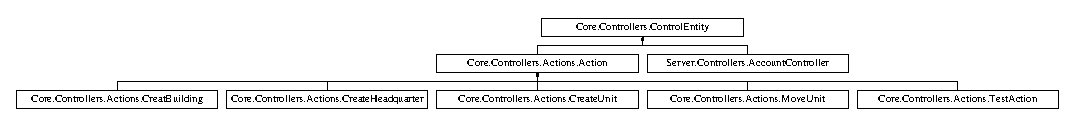
\includegraphics[height=1.235294cm]{classCore_1_1Controllers_1_1ControlEntity}
\end{center}
\end{figure}
\subsection*{Public Member Functions}
\begin{DoxyCompactItemize}
\item 
\hypertarget{classCore_1_1Controllers_1_1ControlEntity_ae658365fdb72c178ad05c27d258fcca2}{{\bfseries Control\-Entity} (\hyperlink{classCore_1_1Models_1_1ModelEntity}{Core.\-Models.\-Model\-Entity} model)}\label{classCore_1_1Controllers_1_1ControlEntity_ae658365fdb72c178ad05c27d258fcca2}

\end{DoxyCompactItemize}
\subsection*{Properties}
\begin{DoxyCompactItemize}
\item 
\hypertarget{classCore_1_1Controllers_1_1ControlEntity_ad5b9626748577b6af9b63c5d83e7739a}{\hyperlink{classCore_1_1Models_1_1ModelEntity}{Core.\-Models.\-Model\-Entity} {\bfseries Model}\hspace{0.3cm}{\ttfamily  \mbox{[}get, set\mbox{]}}}\label{classCore_1_1Controllers_1_1ControlEntity_ad5b9626748577b6af9b63c5d83e7739a}

\end{DoxyCompactItemize}


\subsection{Detailed Description}
M\-V\-C \hyperlink{classCore_1_1Controllers_1_1Controller}{Controller}. 



The documentation for this class was generated from the following file\-:\begin{DoxyCompactItemize}
\item 
base/\-Controllers/Control\-Entity.\-cs\end{DoxyCompactItemize}

\hypertarget{classCore_1_1Controllers_1_1Controller}{\section{Core.\-Controllers.\-Controller Class Reference}
\label{classCore_1_1Controllers_1_1Controller}\index{Core.\-Controllers.\-Controller@{Core.\-Controllers.\-Controller}}
}
\subsection*{Public Attributes}
\begin{DoxyCompactItemize}
\item 
\hypertarget{classCore_1_1Controllers_1_1Controller_a13c0a9251d550621898cffbfcfc732a7}{\hyperlink{classCore_1_1Controllers_1_1RegionManagerController}{Region\-Manager\-Controller} {\bfseries Region\-Manager\-Controller}}\label{classCore_1_1Controllers_1_1Controller_a13c0a9251d550621898cffbfcfc732a7}

\item 
\hypertarget{classCore_1_1Controllers_1_1Controller_a607c9eb803a7f9ec2e60b96827ef26ae}{\hyperlink{classCore_1_1Controllers_1_1DefinitionManagerController}{Definition\-Manager\-Controller} {\bfseries Definition\-Manager\-Controller}}\label{classCore_1_1Controllers_1_1Controller_a607c9eb803a7f9ec2e60b96827ef26ae}

\end{DoxyCompactItemize}
\subsection*{Properties}
\begin{DoxyCompactItemize}
\item 
\hypertarget{classCore_1_1Controllers_1_1Controller_a083108465e3ad1fc6ccdd7f0c20ef5cb}{static \hyperlink{classCore_1_1Controllers_1_1Controller}{Controller} {\bfseries Instance}\hspace{0.3cm}{\ttfamily  \mbox{[}get\mbox{]}}}\label{classCore_1_1Controllers_1_1Controller_a083108465e3ad1fc6ccdd7f0c20ef5cb}

\end{DoxyCompactItemize}


The documentation for this class was generated from the following file\-:\begin{DoxyCompactItemize}
\item 
base/\-Controllers/Controller.\-cs\end{DoxyCompactItemize}

\hypertarget{classCore_1_1Controllers_1_1Actions_1_1CreatBuilding}{\section{Core.\-Controllers.\-Actions.\-Creat\-Building Class Reference}
\label{classCore_1_1Controllers_1_1Actions_1_1CreatBuilding}\index{Core.\-Controllers.\-Actions.\-Creat\-Building@{Core.\-Controllers.\-Actions.\-Creat\-Building}}
}
Inheritance diagram for Core.\-Controllers.\-Actions.\-Creat\-Building\-:\begin{figure}[H]
\begin{center}
\leavevmode
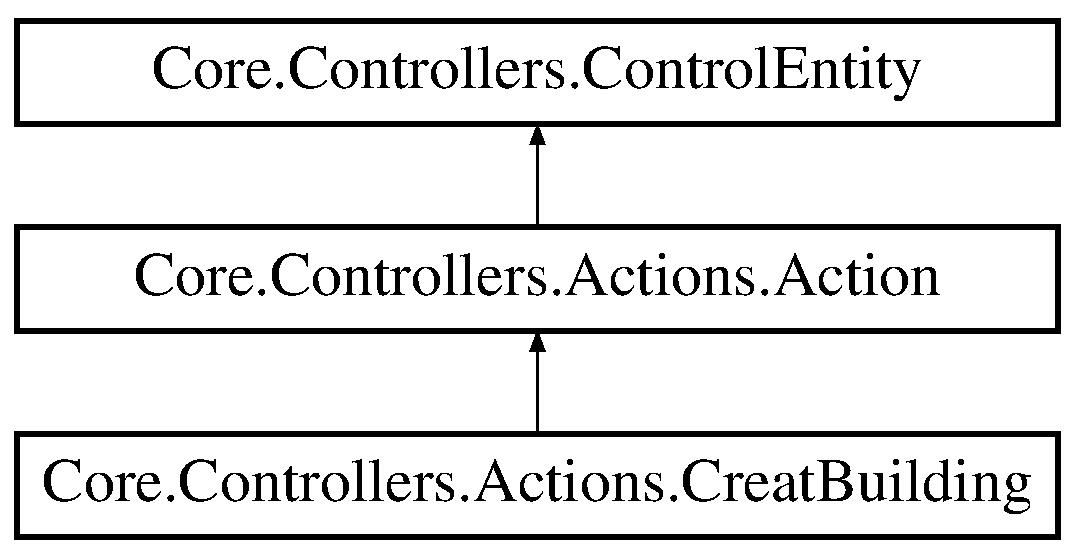
\includegraphics[height=3.000000cm]{classCore_1_1Controllers_1_1Actions_1_1CreatBuilding}
\end{center}
\end{figure}
\subsection*{Public Member Functions}
\begin{DoxyCompactItemize}
\item 
\hyperlink{classCore_1_1Controllers_1_1Actions_1_1CreatBuilding_ab9867559b36ad20f4b9add3cecc9df0a}{Creat\-Building} (\hyperlink{classCore_1_1Models_1_1ModelEntity}{Core.\-Models.\-Model\-Entity} model)
\begin{DoxyCompactList}\small\item\em Constructor of the class \hyperlink{classCore_1_1Controllers_1_1Actions_1_1CreateHeadquarter}{Create\-Headquarter}. \end{DoxyCompactList}\item 
override Concurrent\-Bag\\*
$<$ \hyperlink{classCore_1_1Models_1_1Region}{Core.\-Models.\-Region} $>$ \hyperlink{classCore_1_1Controllers_1_1Actions_1_1CreatBuilding_a5bf6ef12c81df393d3bff87f129cb5f5}{Get\-Affected\-Regions} ()
\begin{DoxyCompactList}\small\item\em Identify the affected region by this action. \end{DoxyCompactList}\item 
override bool \hyperlink{classCore_1_1Controllers_1_1Actions_1_1CreatBuilding_a10b4bb58784bd5da25abac85727e30b0}{Possible} ()
\begin{DoxyCompactList}\small\item\em Returns if the action is even possible. \end{DoxyCompactList}\item 
override Concurrent\-Bag\\*
$<$ \hyperlink{classCore_1_1Models_1_1Region}{Core.\-Models.\-Region} $>$ \hyperlink{classCore_1_1Controllers_1_1Actions_1_1CreatBuilding_a9592b18efa8b8fa114fb3900c5880f06}{Do} ()
\begin{DoxyCompactList}\small\item\em Apply action-\/related changes to the world. \end{DoxyCompactList}\item 
override bool \hyperlink{classCore_1_1Controllers_1_1Actions_1_1CreatBuilding_a697d2c89ef9823be8c5601ff789ea879}{Catch} ()
\begin{DoxyCompactList}\small\item\em In case of errors, revert the world data to a valid state. \end{DoxyCompactList}\item 
override \hyperlink{classCore_1_1Models_1_1RegionPosition}{Core.\-Models.\-Region\-Position} \hyperlink{classCore_1_1Controllers_1_1Actions_1_1CreatBuilding_a03023385415b401cc3361d8b37d13899}{Get\-Region\-Position} ()
\begin{DoxyCompactList}\small\item\em Overide base.\-model.\-Region\-Position class and return the position\-I of the region. \end{DoxyCompactList}\end{DoxyCompactItemize}
\subsection*{Public Attributes}
\begin{DoxyCompactItemize}
\item 
\hypertarget{classCore_1_1Controllers_1_1Actions_1_1CreatBuilding_a6b4126538ce8f230433b21e732b1d59b}{const string {\bfseries C\-R\-E\-A\-T\-E\-\_\-\-P\-O\-S\-I\-T\-I\-O\-N} = \char`\"{}Create\-Position\char`\"{}}\label{classCore_1_1Controllers_1_1Actions_1_1CreatBuilding_a6b4126538ce8f230433b21e732b1d59b}

\item 
\hypertarget{classCore_1_1Controllers_1_1Actions_1_1CreatBuilding_acdf27490ec9e6d72d9c86f1ac0df5641}{const string {\bfseries C\-R\-E\-A\-T\-I\-O\-N\-\_\-\-T\-Y\-P\-E} = \char`\"{}Create\-Building\char`\"{}}\label{classCore_1_1Controllers_1_1Actions_1_1CreatBuilding_acdf27490ec9e6d72d9c86f1ac0df5641}

\end{DoxyCompactItemize}
\subsection*{Additional Inherited Members}


\subsection{Constructor \& Destructor Documentation}
\hypertarget{classCore_1_1Controllers_1_1Actions_1_1CreatBuilding_ab9867559b36ad20f4b9add3cecc9df0a}{\index{Core\-::\-Controllers\-::\-Actions\-::\-Creat\-Building@{Core\-::\-Controllers\-::\-Actions\-::\-Creat\-Building}!Creat\-Building@{Creat\-Building}}
\index{Creat\-Building@{Creat\-Building}!Core::Controllers::Actions::CreatBuilding@{Core\-::\-Controllers\-::\-Actions\-::\-Creat\-Building}}
\subsubsection[{Creat\-Building}]{\setlength{\rightskip}{0pt plus 5cm}Core.\-Controllers.\-Actions.\-Creat\-Building.\-Creat\-Building (
\begin{DoxyParamCaption}
\item[{{\bf Core.\-Models.\-Model\-Entity}}]{model}
\end{DoxyParamCaption}
)\hspace{0.3cm}{\ttfamily [inline]}}}\label{classCore_1_1Controllers_1_1Actions_1_1CreatBuilding_ab9867559b36ad20f4b9add3cecc9df0a}


Constructor of the class \hyperlink{classCore_1_1Controllers_1_1Actions_1_1CreateHeadquarter}{Create\-Headquarter}. 


\begin{DoxyParams}{Parameters}
{\em model} & \\
\hline
\end{DoxyParams}


\subsection{Member Function Documentation}
\hypertarget{classCore_1_1Controllers_1_1Actions_1_1CreatBuilding_a697d2c89ef9823be8c5601ff789ea879}{\index{Core\-::\-Controllers\-::\-Actions\-::\-Creat\-Building@{Core\-::\-Controllers\-::\-Actions\-::\-Creat\-Building}!Catch@{Catch}}
\index{Catch@{Catch}!Core::Controllers::Actions::CreatBuilding@{Core\-::\-Controllers\-::\-Actions\-::\-Creat\-Building}}
\subsubsection[{Catch}]{\setlength{\rightskip}{0pt plus 5cm}override bool Core.\-Controllers.\-Actions.\-Creat\-Building.\-Catch (
\begin{DoxyParamCaption}
{}
\end{DoxyParamCaption}
)\hspace{0.3cm}{\ttfamily [inline]}, {\ttfamily [virtual]}}}\label{classCore_1_1Controllers_1_1Actions_1_1CreatBuilding_a697d2c89ef9823be8c5601ff789ea879}


In case of errors, revert the world data to a valid state. 


\begin{DoxyParams}{Parameters}
{\em region\-Manager\-C} & \\
\hline
\end{DoxyParams}
\begin{DoxyReturn}{Returns}

\end{DoxyReturn}


Reimplemented from \hyperlink{classCore_1_1Controllers_1_1Actions_1_1Action_ada4c77dfeee78ded10a6eb6a506defb4}{Core.\-Controllers.\-Actions.\-Action}.

\hypertarget{classCore_1_1Controllers_1_1Actions_1_1CreatBuilding_a9592b18efa8b8fa114fb3900c5880f06}{\index{Core\-::\-Controllers\-::\-Actions\-::\-Creat\-Building@{Core\-::\-Controllers\-::\-Actions\-::\-Creat\-Building}!Do@{Do}}
\index{Do@{Do}!Core::Controllers::Actions::CreatBuilding@{Core\-::\-Controllers\-::\-Actions\-::\-Creat\-Building}}
\subsubsection[{Do}]{\setlength{\rightskip}{0pt plus 5cm}override Concurrent\-Bag$<${\bf Core.\-Models.\-Region}$>$ Core.\-Controllers.\-Actions.\-Creat\-Building.\-Do (
\begin{DoxyParamCaption}
{}
\end{DoxyParamCaption}
)\hspace{0.3cm}{\ttfamily [inline]}, {\ttfamily [virtual]}}}\label{classCore_1_1Controllers_1_1Actions_1_1CreatBuilding_a9592b18efa8b8fa114fb3900c5880f06}


Apply action-\/related changes to the world. 


\begin{DoxyParams}{Parameters}
{\em region\-Manager\-C} & \\
\hline
\end{DoxyParams}
\begin{DoxyReturn}{Returns}
Returns System.\-Collections.\-Concurrent.\-Concurrent\-Bag$<$t$>$ class with the affected region./$>$
\end{DoxyReturn}


Reimplemented from \hyperlink{classCore_1_1Controllers_1_1Actions_1_1Action_afbb091ee28eee896951fac600188d446}{Core.\-Controllers.\-Actions.\-Action}.

\hypertarget{classCore_1_1Controllers_1_1Actions_1_1CreatBuilding_a5bf6ef12c81df393d3bff87f129cb5f5}{\index{Core\-::\-Controllers\-::\-Actions\-::\-Creat\-Building@{Core\-::\-Controllers\-::\-Actions\-::\-Creat\-Building}!Get\-Affected\-Regions@{Get\-Affected\-Regions}}
\index{Get\-Affected\-Regions@{Get\-Affected\-Regions}!Core::Controllers::Actions::CreatBuilding@{Core\-::\-Controllers\-::\-Actions\-::\-Creat\-Building}}
\subsubsection[{Get\-Affected\-Regions}]{\setlength{\rightskip}{0pt plus 5cm}override Concurrent\-Bag$<${\bf Core.\-Models.\-Region}$>$ Core.\-Controllers.\-Actions.\-Creat\-Building.\-Get\-Affected\-Regions (
\begin{DoxyParamCaption}
{}
\end{DoxyParamCaption}
)\hspace{0.3cm}{\ttfamily [inline]}, {\ttfamily [virtual]}}}\label{classCore_1_1Controllers_1_1Actions_1_1CreatBuilding_a5bf6ef12c81df393d3bff87f129cb5f5}


Identify the affected region by this action. 


\begin{DoxyParams}{Parameters}
{\em region\-Manager\-C} & Access to maybe changed Regions.\\
\hline
\end{DoxyParams}
\begin{DoxyReturn}{Returns}
Returns System.\-Collections.\-Concurrent.\-Concurrent\-Bag$<$t$>$ with the affected region. 
\end{DoxyReturn}


Reimplemented from \hyperlink{classCore_1_1Controllers_1_1Actions_1_1Action_aa11bdeffff43ec47ac7c3d6843a85674}{Core.\-Controllers.\-Actions.\-Action}.

\hypertarget{classCore_1_1Controllers_1_1Actions_1_1CreatBuilding_a03023385415b401cc3361d8b37d13899}{\index{Core\-::\-Controllers\-::\-Actions\-::\-Creat\-Building@{Core\-::\-Controllers\-::\-Actions\-::\-Creat\-Building}!Get\-Region\-Position@{Get\-Region\-Position}}
\index{Get\-Region\-Position@{Get\-Region\-Position}!Core::Controllers::Actions::CreatBuilding@{Core\-::\-Controllers\-::\-Actions\-::\-Creat\-Building}}
\subsubsection[{Get\-Region\-Position}]{\setlength{\rightskip}{0pt plus 5cm}override {\bf Core.\-Models.\-Region\-Position} Core.\-Controllers.\-Actions.\-Creat\-Building.\-Get\-Region\-Position (
\begin{DoxyParamCaption}
{}
\end{DoxyParamCaption}
)\hspace{0.3cm}{\ttfamily [inline]}, {\ttfamily [virtual]}}}\label{classCore_1_1Controllers_1_1Actions_1_1CreatBuilding_a03023385415b401cc3361d8b37d13899}


Overide base.\-model.\-Region\-Position class and return the position\-I of the region. 

\begin{DoxyReturn}{Returns}
The region position.
\end{DoxyReturn}


Reimplemented from \hyperlink{classCore_1_1Controllers_1_1Actions_1_1Action_a6ffe3c30cb5648a81f50096f4f332d5a}{Core.\-Controllers.\-Actions.\-Action}.

\hypertarget{classCore_1_1Controllers_1_1Actions_1_1CreatBuilding_a10b4bb58784bd5da25abac85727e30b0}{\index{Core\-::\-Controllers\-::\-Actions\-::\-Creat\-Building@{Core\-::\-Controllers\-::\-Actions\-::\-Creat\-Building}!Possible@{Possible}}
\index{Possible@{Possible}!Core::Controllers::Actions::CreatBuilding@{Core\-::\-Controllers\-::\-Actions\-::\-Creat\-Building}}
\subsubsection[{Possible}]{\setlength{\rightskip}{0pt plus 5cm}override bool Core.\-Controllers.\-Actions.\-Creat\-Building.\-Possible (
\begin{DoxyParamCaption}
{}
\end{DoxyParamCaption}
)\hspace{0.3cm}{\ttfamily [inline]}, {\ttfamily [virtual]}}}\label{classCore_1_1Controllers_1_1Actions_1_1CreatBuilding_a10b4bb58784bd5da25abac85727e30b0}


Returns if the action is even possible. 


\begin{DoxyParams}{Parameters}
{\em region\-Manager\-C} & \\
\hline
\end{DoxyParams}
\begin{DoxyReturn}{Returns}
True if the Headquarte is buildable at the current position, otherwise false.
\end{DoxyReturn}


Reimplemented from \hyperlink{classCore_1_1Controllers_1_1Actions_1_1Action_a405b995343a9394ad19e05a699a4e6d9}{Core.\-Controllers.\-Actions.\-Action}.



The documentation for this class was generated from the following file\-:\begin{DoxyCompactItemize}
\item 
base/\-Controllers/\-Action/Create\-Building.\-cs\end{DoxyCompactItemize}

\hypertarget{classClient_1_1Common_1_1Views_1_1Actions_1_1CreateBuilding}{}\section{Client.\+Common.\+Views.\+Actions.\+Create\+Building Class Reference}
\label{classClient_1_1Common_1_1Views_1_1Actions_1_1CreateBuilding}\index{Client.\+Common.\+Views.\+Actions.\+Create\+Building@{Client.\+Common.\+Views.\+Actions.\+Create\+Building}}


Create a building.  


Inheritance diagram for Client.\+Common.\+Views.\+Actions.\+Create\+Building\+:\begin{figure}[H]
\begin{center}
\leavevmode
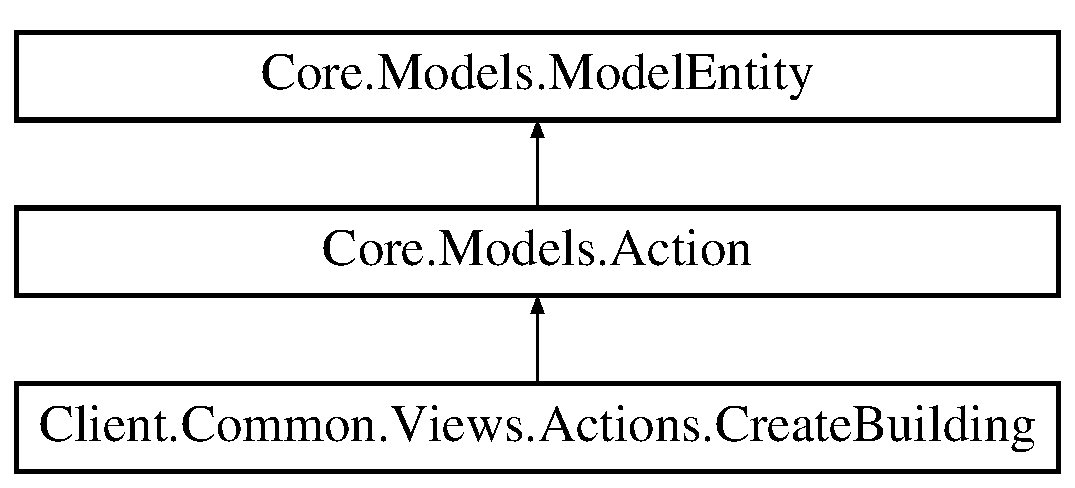
\includegraphics[height=3.000000cm]{classClient_1_1Common_1_1Views_1_1Actions_1_1CreateBuilding}
\end{center}
\end{figure}
\subsection*{Public Member Functions}
\begin{DoxyCompactItemize}
\item 
\hyperlink{classClient_1_1Common_1_1Views_1_1Actions_1_1CreateBuilding_a2f4fe0e79bc911291d5b69f0754efc3a}{Create\+Building} (\hyperlink{classCore_1_1Models_1_1ModelEntity}{Core.\+Models.\+Model\+Entity} model, \hyperlink{classClient_1_1Common_1_1Views_1_1RegionViewHex}{Region\+View\+Hex} region\+View\+Hex)
\begin{DoxyCompactList}\small\item\em Initializes a new instance of the \hyperlink{classClient_1_1Common_1_1Views_1_1Actions_1_1CreateBuilding}{Client.\+Common.\+Views.\+Actions.\+Create\+Building} class. \end{DoxyCompactList}\item 
override void \hyperlink{classClient_1_1Common_1_1Views_1_1Actions_1_1CreateBuilding_ac4ae114e1751a82e521cb3dfbc346e49}{Before\+Do} ()
\begin{DoxyCompactList}\small\item\em Gets called before Action\+Control.\+Do() gets executed. Should get and store data which will be needed in Schedule. \end{DoxyCompactList}\item 
override bool \hyperlink{classClient_1_1Common_1_1Views_1_1Actions_1_1CreateBuilding_a9124e0ed7b33ef3b674613b9dbda626f}{Schedule} (float frame\+Times\+In\+Second)
\begin{DoxyCompactList}\small\item\em Schedules the action. Should do anything do animate the action (e.\+g. draw the entity, animate his moving or start/end animating a fight) Returns true if the action has ended, otherwise false. \end{DoxyCompactList}\end{DoxyCompactItemize}
\subsection*{Properties}
\begin{DoxyCompactItemize}
\item 
\hyperlink{classClient_1_1Common_1_1Views_1_1RegionViewHex}{Region\+View\+Hex} \hyperlink{classClient_1_1Common_1_1Views_1_1Actions_1_1CreateBuilding_ab73f911ae98f56d040a6eb03e50f451f}{Region\+View\+Hex}\hspace{0.3cm}{\ttfamily  \mbox{[}get\mbox{]}}
\begin{DoxyCompactList}\small\item\em Gets the world layer. \end{DoxyCompactList}\end{DoxyCompactItemize}
\subsection*{Additional Inherited Members}


\subsection{Detailed Description}
Create a building. 



\subsection{Constructor \& Destructor Documentation}
\hypertarget{classClient_1_1Common_1_1Views_1_1Actions_1_1CreateBuilding_a2f4fe0e79bc911291d5b69f0754efc3a}{}\index{Client\+::\+Common\+::\+Views\+::\+Actions\+::\+Create\+Building@{Client\+::\+Common\+::\+Views\+::\+Actions\+::\+Create\+Building}!Create\+Building@{Create\+Building}}
\index{Create\+Building@{Create\+Building}!Client\+::\+Common\+::\+Views\+::\+Actions\+::\+Create\+Building@{Client\+::\+Common\+::\+Views\+::\+Actions\+::\+Create\+Building}}
\subsubsection[{Create\+Building(\+Core.\+Models.\+Model\+Entity model, Region\+View\+Hex region\+View\+Hex)}]{\setlength{\rightskip}{0pt plus 5cm}Client.\+Common.\+Views.\+Actions.\+Create\+Building.\+Create\+Building (
\begin{DoxyParamCaption}
\item[{{\bf Core.\+Models.\+Model\+Entity}}]{model, }
\item[{{\bf Region\+View\+Hex}}]{region\+View\+Hex}
\end{DoxyParamCaption}
)}\label{classClient_1_1Common_1_1Views_1_1Actions_1_1CreateBuilding_a2f4fe0e79bc911291d5b69f0754efc3a}


Initializes a new instance of the \hyperlink{classClient_1_1Common_1_1Views_1_1Actions_1_1CreateBuilding}{Client.\+Common.\+Views.\+Actions.\+Create\+Building} class. 


\begin{DoxyParams}{Parameters}
{\em model} & Model of the Building\\
\hline
{\em region\+View\+Hex} & World layer.\\
\hline
\end{DoxyParams}


\subsection{Member Function Documentation}
\hypertarget{classClient_1_1Common_1_1Views_1_1Actions_1_1CreateBuilding_ac4ae114e1751a82e521cb3dfbc346e49}{}\index{Client\+::\+Common\+::\+Views\+::\+Actions\+::\+Create\+Building@{Client\+::\+Common\+::\+Views\+::\+Actions\+::\+Create\+Building}!Before\+Do@{Before\+Do}}
\index{Before\+Do@{Before\+Do}!Client\+::\+Common\+::\+Views\+::\+Actions\+::\+Create\+Building@{Client\+::\+Common\+::\+Views\+::\+Actions\+::\+Create\+Building}}
\subsubsection[{Before\+Do()}]{\setlength{\rightskip}{0pt plus 5cm}override void Client.\+Common.\+Views.\+Actions.\+Create\+Building.\+Before\+Do (
\begin{DoxyParamCaption}
{}
\end{DoxyParamCaption}
)}\label{classClient_1_1Common_1_1Views_1_1Actions_1_1CreateBuilding_ac4ae114e1751a82e521cb3dfbc346e49}


Gets called before Action\+Control.\+Do() gets executed. Should get and store data which will be needed in Schedule. 

\hypertarget{classClient_1_1Common_1_1Views_1_1Actions_1_1CreateBuilding_a9124e0ed7b33ef3b674613b9dbda626f}{}\index{Client\+::\+Common\+::\+Views\+::\+Actions\+::\+Create\+Building@{Client\+::\+Common\+::\+Views\+::\+Actions\+::\+Create\+Building}!Schedule@{Schedule}}
\index{Schedule@{Schedule}!Client\+::\+Common\+::\+Views\+::\+Actions\+::\+Create\+Building@{Client\+::\+Common\+::\+Views\+::\+Actions\+::\+Create\+Building}}
\subsubsection[{Schedule(float frame\+Times\+In\+Second)}]{\setlength{\rightskip}{0pt plus 5cm}override bool Client.\+Common.\+Views.\+Actions.\+Create\+Building.\+Schedule (
\begin{DoxyParamCaption}
\item[{float}]{frame\+Times\+In\+Second}
\end{DoxyParamCaption}
)}\label{classClient_1_1Common_1_1Views_1_1Actions_1_1CreateBuilding_a9124e0ed7b33ef3b674613b9dbda626f}


Schedules the action. Should do anything do animate the action (e.\+g. draw the entity, animate his moving or start/end animating a fight) Returns true if the action has ended, otherwise false. 


\begin{DoxyParams}{Parameters}
{\em frame\+Times\+In\+Second} & frames times in seconds.\\
\hline
\end{DoxyParams}
\begin{DoxyReturn}{Returns}
true if the schedule of the action is done
\end{DoxyReturn}


\subsection{Property Documentation}
\hypertarget{classClient_1_1Common_1_1Views_1_1Actions_1_1CreateBuilding_ab73f911ae98f56d040a6eb03e50f451f}{}\index{Client\+::\+Common\+::\+Views\+::\+Actions\+::\+Create\+Building@{Client\+::\+Common\+::\+Views\+::\+Actions\+::\+Create\+Building}!Region\+View\+Hex@{Region\+View\+Hex}}
\index{Region\+View\+Hex@{Region\+View\+Hex}!Client\+::\+Common\+::\+Views\+::\+Actions\+::\+Create\+Building@{Client\+::\+Common\+::\+Views\+::\+Actions\+::\+Create\+Building}}
\subsubsection[{Region\+View\+Hex}]{\setlength{\rightskip}{0pt plus 5cm}{\bf Region\+View\+Hex} Client.\+Common.\+Views.\+Actions.\+Create\+Building.\+Region\+View\+Hex\hspace{0.3cm}{\ttfamily [get]}}\label{classClient_1_1Common_1_1Views_1_1Actions_1_1CreateBuilding_ab73f911ae98f56d040a6eb03e50f451f}


Gets the world layer. 

The world layer.

The documentation for this class was generated from the following file\+:\begin{DoxyCompactItemize}
\item 
client/client/client.\+Common/\+Views/\+Actions/Create\+Building.\+cs\end{DoxyCompactItemize}

\hypertarget{classCore_1_1Controllers_1_1Actions_1_1CreateHeadquarter}{\section{Core.\-Controllers.\-Actions.\-Create\-Headquarter Class Reference}
\label{classCore_1_1Controllers_1_1Actions_1_1CreateHeadquarter}\index{Core.\-Controllers.\-Actions.\-Create\-Headquarter@{Core.\-Controllers.\-Actions.\-Create\-Headquarter}}
}
Inheritance diagram for Core.\-Controllers.\-Actions.\-Create\-Headquarter\-:\begin{figure}[H]
\begin{center}
\leavevmode
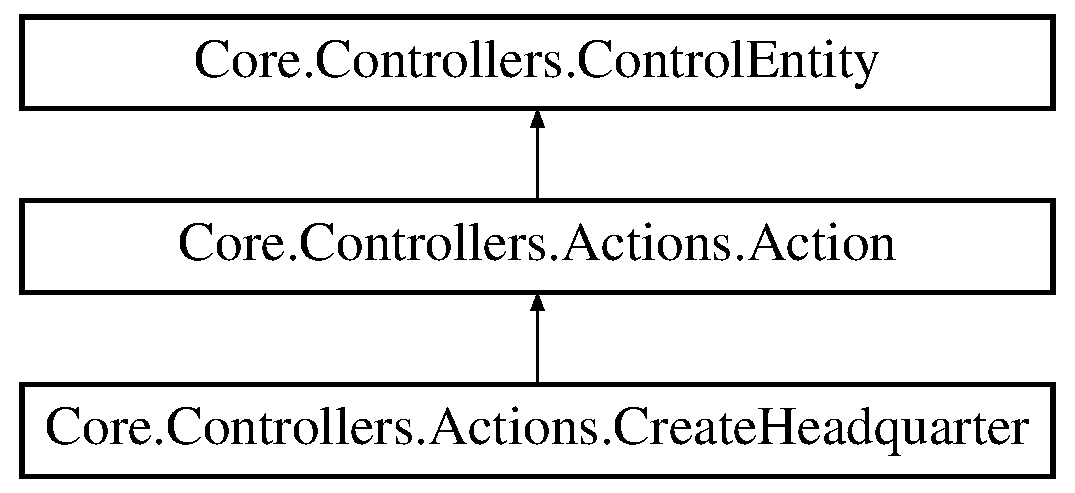
\includegraphics[height=3.000000cm]{classCore_1_1Controllers_1_1Actions_1_1CreateHeadquarter}
\end{center}
\end{figure}
\subsection*{Public Member Functions}
\begin{DoxyCompactItemize}
\item 
\hyperlink{classCore_1_1Controllers_1_1Actions_1_1CreateHeadquarter_a4c0fe65eb8038f6167d9d9fe42834ee8}{Create\-Headquarter} (\hyperlink{classCore_1_1Models_1_1ModelEntity}{Core.\-Models.\-Model\-Entity} model)
\begin{DoxyCompactList}\small\item\em Constructor of the class \hyperlink{classCore_1_1Controllers_1_1Actions_1_1CreateHeadquarter}{Create\-Headquarter}. \end{DoxyCompactList}\item 
override Concurrent\-Bag\\*
$<$ \hyperlink{classCore_1_1Models_1_1Region}{Core.\-Models.\-Region} $>$ \hyperlink{classCore_1_1Controllers_1_1Actions_1_1CreateHeadquarter_a2d0e5c9eaa6f539581c62f649e76fce7}{Get\-Affected\-Regions} ()
\begin{DoxyCompactList}\small\item\em Identify the affected region by this action. \end{DoxyCompactList}\item 
override bool \hyperlink{classCore_1_1Controllers_1_1Actions_1_1CreateHeadquarter_aae428d8792453bea4aae8dfd9478a1fd}{Possible} ()
\begin{DoxyCompactList}\small\item\em Returns if the action is even possible. \end{DoxyCompactList}\item 
override Concurrent\-Bag\\*
$<$ \hyperlink{classCore_1_1Models_1_1Region}{Core.\-Models.\-Region} $>$ \hyperlink{classCore_1_1Controllers_1_1Actions_1_1CreateHeadquarter_af17ed42c13d869322a61adac0b1911a4}{Do} ()
\begin{DoxyCompactList}\small\item\em Apply action-\/related changes to the world. \end{DoxyCompactList}\item 
override bool \hyperlink{classCore_1_1Controllers_1_1Actions_1_1CreateHeadquarter_a1784d785515ab957f3f634c2907908d5}{Catch} ()
\begin{DoxyCompactList}\small\item\em In case of errors, revert the world data to a valid state. \end{DoxyCompactList}\item 
override \hyperlink{classCore_1_1Models_1_1RegionPosition}{Core.\-Models.\-Region\-Position} \hyperlink{classCore_1_1Controllers_1_1Actions_1_1CreateHeadquarter_aafbd900bc7a38f4268f00f57078d4b4a}{Get\-Region\-Position} ()
\begin{DoxyCompactList}\small\item\em Ovveride base.\-model.\-Region\-Position class and return the position\-I of the region. \end{DoxyCompactList}\end{DoxyCompactItemize}
\subsection*{Public Attributes}
\begin{DoxyCompactItemize}
\item 
\hypertarget{classCore_1_1Controllers_1_1Actions_1_1CreateHeadquarter_aa1a0efceff1050f3b8ba160629379a0b}{const string {\bfseries C\-R\-E\-A\-T\-E\-\_\-\-P\-O\-S\-I\-T\-I\-O\-N} = \char`\"{}Create\-Position\char`\"{}}\label{classCore_1_1Controllers_1_1Actions_1_1CreateHeadquarter_aa1a0efceff1050f3b8ba160629379a0b}

\end{DoxyCompactItemize}
\subsection*{Additional Inherited Members}


\subsection{Constructor \& Destructor Documentation}
\hypertarget{classCore_1_1Controllers_1_1Actions_1_1CreateHeadquarter_a4c0fe65eb8038f6167d9d9fe42834ee8}{\index{Core\-::\-Controllers\-::\-Actions\-::\-Create\-Headquarter@{Core\-::\-Controllers\-::\-Actions\-::\-Create\-Headquarter}!Create\-Headquarter@{Create\-Headquarter}}
\index{Create\-Headquarter@{Create\-Headquarter}!Core::Controllers::Actions::CreateHeadquarter@{Core\-::\-Controllers\-::\-Actions\-::\-Create\-Headquarter}}
\subsubsection[{Create\-Headquarter}]{\setlength{\rightskip}{0pt plus 5cm}Core.\-Controllers.\-Actions.\-Create\-Headquarter.\-Create\-Headquarter (
\begin{DoxyParamCaption}
\item[{{\bf Core.\-Models.\-Model\-Entity}}]{model}
\end{DoxyParamCaption}
)\hspace{0.3cm}{\ttfamily [inline]}}}\label{classCore_1_1Controllers_1_1Actions_1_1CreateHeadquarter_a4c0fe65eb8038f6167d9d9fe42834ee8}


Constructor of the class \hyperlink{classCore_1_1Controllers_1_1Actions_1_1CreateHeadquarter}{Create\-Headquarter}. 


\begin{DoxyParams}{Parameters}
{\em model} & \\
\hline
\end{DoxyParams}


\subsection{Member Function Documentation}
\hypertarget{classCore_1_1Controllers_1_1Actions_1_1CreateHeadquarter_a1784d785515ab957f3f634c2907908d5}{\index{Core\-::\-Controllers\-::\-Actions\-::\-Create\-Headquarter@{Core\-::\-Controllers\-::\-Actions\-::\-Create\-Headquarter}!Catch@{Catch}}
\index{Catch@{Catch}!Core::Controllers::Actions::CreateHeadquarter@{Core\-::\-Controllers\-::\-Actions\-::\-Create\-Headquarter}}
\subsubsection[{Catch}]{\setlength{\rightskip}{0pt plus 5cm}override bool Core.\-Controllers.\-Actions.\-Create\-Headquarter.\-Catch (
\begin{DoxyParamCaption}
{}
\end{DoxyParamCaption}
)\hspace{0.3cm}{\ttfamily [inline]}, {\ttfamily [virtual]}}}\label{classCore_1_1Controllers_1_1Actions_1_1CreateHeadquarter_a1784d785515ab957f3f634c2907908d5}


In case of errors, revert the world data to a valid state. 


\begin{DoxyParams}{Parameters}
{\em region\-Manager\-C} & \\
\hline
\end{DoxyParams}
\begin{DoxyReturn}{Returns}

\end{DoxyReturn}


Reimplemented from \hyperlink{classCore_1_1Controllers_1_1Actions_1_1Action_ada4c77dfeee78ded10a6eb6a506defb4}{Core.\-Controllers.\-Actions.\-Action}.

\hypertarget{classCore_1_1Controllers_1_1Actions_1_1CreateHeadquarter_af17ed42c13d869322a61adac0b1911a4}{\index{Core\-::\-Controllers\-::\-Actions\-::\-Create\-Headquarter@{Core\-::\-Controllers\-::\-Actions\-::\-Create\-Headquarter}!Do@{Do}}
\index{Do@{Do}!Core::Controllers::Actions::CreateHeadquarter@{Core\-::\-Controllers\-::\-Actions\-::\-Create\-Headquarter}}
\subsubsection[{Do}]{\setlength{\rightskip}{0pt plus 5cm}override Concurrent\-Bag$<${\bf Core.\-Models.\-Region}$>$ Core.\-Controllers.\-Actions.\-Create\-Headquarter.\-Do (
\begin{DoxyParamCaption}
{}
\end{DoxyParamCaption}
)\hspace{0.3cm}{\ttfamily [inline]}, {\ttfamily [virtual]}}}\label{classCore_1_1Controllers_1_1Actions_1_1CreateHeadquarter_af17ed42c13d869322a61adac0b1911a4}


Apply action-\/related changes to the world. 


\begin{DoxyParams}{Parameters}
{\em region\-Manager\-C} & \\
\hline
\end{DoxyParams}
\begin{DoxyReturn}{Returns}
Returns System.\-Collections.\-Concurrent.\-Concurrent\-Bag$<$t$>$ class with the affected region./$>$
\end{DoxyReturn}


Reimplemented from \hyperlink{classCore_1_1Controllers_1_1Actions_1_1Action_afbb091ee28eee896951fac600188d446}{Core.\-Controllers.\-Actions.\-Action}.

\hypertarget{classCore_1_1Controllers_1_1Actions_1_1CreateHeadquarter_a2d0e5c9eaa6f539581c62f649e76fce7}{\index{Core\-::\-Controllers\-::\-Actions\-::\-Create\-Headquarter@{Core\-::\-Controllers\-::\-Actions\-::\-Create\-Headquarter}!Get\-Affected\-Regions@{Get\-Affected\-Regions}}
\index{Get\-Affected\-Regions@{Get\-Affected\-Regions}!Core::Controllers::Actions::CreateHeadquarter@{Core\-::\-Controllers\-::\-Actions\-::\-Create\-Headquarter}}
\subsubsection[{Get\-Affected\-Regions}]{\setlength{\rightskip}{0pt plus 5cm}override Concurrent\-Bag$<${\bf Core.\-Models.\-Region}$>$ Core.\-Controllers.\-Actions.\-Create\-Headquarter.\-Get\-Affected\-Regions (
\begin{DoxyParamCaption}
{}
\end{DoxyParamCaption}
)\hspace{0.3cm}{\ttfamily [inline]}, {\ttfamily [virtual]}}}\label{classCore_1_1Controllers_1_1Actions_1_1CreateHeadquarter_a2d0e5c9eaa6f539581c62f649e76fce7}


Identify the affected region by this action. 


\begin{DoxyParams}{Parameters}
{\em region\-Manager\-C} & Access to maybe changed Regions.\\
\hline
\end{DoxyParams}
\begin{DoxyReturn}{Returns}
Returns System.\-Collections.\-Concurrent.\-Concurrent\-Bag$<$t$>$ with the affected region. 
\end{DoxyReturn}


Reimplemented from \hyperlink{classCore_1_1Controllers_1_1Actions_1_1Action_aa11bdeffff43ec47ac7c3d6843a85674}{Core.\-Controllers.\-Actions.\-Action}.

\hypertarget{classCore_1_1Controllers_1_1Actions_1_1CreateHeadquarter_aafbd900bc7a38f4268f00f57078d4b4a}{\index{Core\-::\-Controllers\-::\-Actions\-::\-Create\-Headquarter@{Core\-::\-Controllers\-::\-Actions\-::\-Create\-Headquarter}!Get\-Region\-Position@{Get\-Region\-Position}}
\index{Get\-Region\-Position@{Get\-Region\-Position}!Core::Controllers::Actions::CreateHeadquarter@{Core\-::\-Controllers\-::\-Actions\-::\-Create\-Headquarter}}
\subsubsection[{Get\-Region\-Position}]{\setlength{\rightskip}{0pt plus 5cm}override {\bf Core.\-Models.\-Region\-Position} Core.\-Controllers.\-Actions.\-Create\-Headquarter.\-Get\-Region\-Position (
\begin{DoxyParamCaption}
{}
\end{DoxyParamCaption}
)\hspace{0.3cm}{\ttfamily [inline]}, {\ttfamily [virtual]}}}\label{classCore_1_1Controllers_1_1Actions_1_1CreateHeadquarter_aafbd900bc7a38f4268f00f57078d4b4a}


Ovveride base.\-model.\-Region\-Position class and return the position\-I of the region. 

\begin{DoxyReturn}{Returns}

\end{DoxyReturn}


Reimplemented from \hyperlink{classCore_1_1Controllers_1_1Actions_1_1Action_a6ffe3c30cb5648a81f50096f4f332d5a}{Core.\-Controllers.\-Actions.\-Action}.

\hypertarget{classCore_1_1Controllers_1_1Actions_1_1CreateHeadquarter_aae428d8792453bea4aae8dfd9478a1fd}{\index{Core\-::\-Controllers\-::\-Actions\-::\-Create\-Headquarter@{Core\-::\-Controllers\-::\-Actions\-::\-Create\-Headquarter}!Possible@{Possible}}
\index{Possible@{Possible}!Core::Controllers::Actions::CreateHeadquarter@{Core\-::\-Controllers\-::\-Actions\-::\-Create\-Headquarter}}
\subsubsection[{Possible}]{\setlength{\rightskip}{0pt plus 5cm}override bool Core.\-Controllers.\-Actions.\-Create\-Headquarter.\-Possible (
\begin{DoxyParamCaption}
{}
\end{DoxyParamCaption}
)\hspace{0.3cm}{\ttfamily [inline]}, {\ttfamily [virtual]}}}\label{classCore_1_1Controllers_1_1Actions_1_1CreateHeadquarter_aae428d8792453bea4aae8dfd9478a1fd}


Returns if the action is even possible. 


\begin{DoxyParams}{Parameters}
{\em region\-Manager\-C} & \\
\hline
\end{DoxyParams}
\begin{DoxyReturn}{Returns}
True if the Headquarte is buildable at the current position, otherwise false.
\end{DoxyReturn}


Reimplemented from \hyperlink{classCore_1_1Controllers_1_1Actions_1_1Action_a405b995343a9394ad19e05a699a4e6d9}{Core.\-Controllers.\-Actions.\-Action}.



The documentation for this class was generated from the following file\-:\begin{DoxyCompactItemize}
\item 
base/\-Controllers/\-Action/Create\-Headquarter.\-cs\end{DoxyCompactItemize}

\hypertarget{classSQLite_1_1CreateTablesResult}{}\section{S\+Q\+Lite.\+Create\+Tables\+Result Class Reference}
\label{classSQLite_1_1CreateTablesResult}\index{S\+Q\+Lite.\+Create\+Tables\+Result@{S\+Q\+Lite.\+Create\+Tables\+Result}}
\subsection*{Properties}
\begin{DoxyCompactItemize}
\item 
\hypertarget{classSQLite_1_1CreateTablesResult_a570a918ea3d12d83f8dd1e2116c818c5}{}Dictionary$<$ Type, int $>$ {\bfseries Results}\hspace{0.3cm}{\ttfamily  \mbox{[}get\mbox{]}}\label{classSQLite_1_1CreateTablesResult_a570a918ea3d12d83f8dd1e2116c818c5}

\end{DoxyCompactItemize}


The documentation for this class was generated from the following file\+:\begin{DoxyCompactItemize}
\item 
packages/sqlite-\/net.\+1.\+0.\+8/content/S\+Q\+Lite\+Async.\+cs\end{DoxyCompactItemize}

\hypertarget{classClient_1_1Common_1_1Views_1_1Actions_1_1CreateUnit}{}\section{Client.\+Common.\+Views.\+Actions.\+Create\+Unit Class Reference}
\label{classClient_1_1Common_1_1Views_1_1Actions_1_1CreateUnit}\index{Client.\+Common.\+Views.\+Actions.\+Create\+Unit@{Client.\+Common.\+Views.\+Actions.\+Create\+Unit}}


Create a unit.  


Inheritance diagram for Client.\+Common.\+Views.\+Actions.\+Create\+Unit\+:\begin{figure}[H]
\begin{center}
\leavevmode
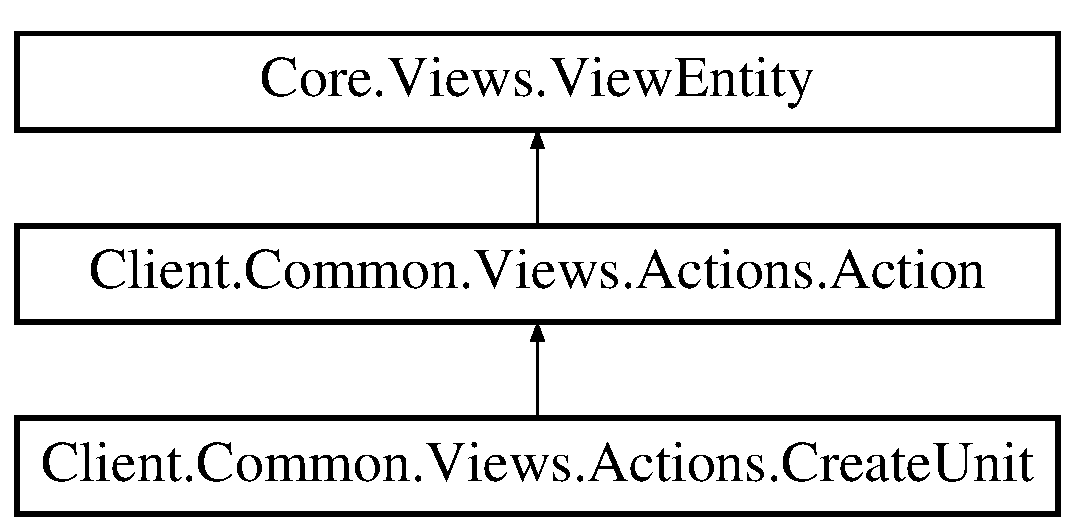
\includegraphics[height=3.000000cm]{classClient_1_1Common_1_1Views_1_1Actions_1_1CreateUnit}
\end{center}
\end{figure}
\subsection*{Public Member Functions}
\begin{DoxyCompactItemize}
\item 
\hyperlink{classClient_1_1Common_1_1Views_1_1Actions_1_1CreateUnit_a4bbc3eb3130b3fdb43877133acb5541e}{Create\+Unit} (\hyperlink{classCore_1_1Models_1_1ModelEntity}{Core.\+Models.\+Model\+Entity} model)
\begin{DoxyCompactList}\small\item\em Initializes a new instance of the \hyperlink{classClient_1_1Common_1_1Views_1_1Actions_1_1CreateUnit}{Client.\+Common.\+Views.\+Actions.\+Create\+Unit} class. \end{DoxyCompactList}\item 
override void \hyperlink{classClient_1_1Common_1_1Views_1_1Actions_1_1CreateUnit_a651d26ad176e10a51065e513eec90aa8}{Before\+Do} ()
\begin{DoxyCompactList}\small\item\em Gets called before Action\+Control.\+Do() gets executed. Should get and store data which will be needed in Schedule. \end{DoxyCompactList}\item 
override bool \hyperlink{classClient_1_1Common_1_1Views_1_1Actions_1_1CreateUnit_a3b0aeac3eabb7b10b3f8fb287bc96181}{Schedule} (float frame\+Times\+In\+Second)
\begin{DoxyCompactList}\small\item\em Schedules the action. Should do anything do animate the action (e.\+g. draw the entity, animate his moving or start/end animating a fight) Returns true if the action has ended, otherwise false. \end{DoxyCompactList}\end{DoxyCompactItemize}
\subsection*{Additional Inherited Members}


\subsection{Detailed Description}
Create a unit. 



\subsection{Constructor \& Destructor Documentation}
\hypertarget{classClient_1_1Common_1_1Views_1_1Actions_1_1CreateUnit_a4bbc3eb3130b3fdb43877133acb5541e}{}\index{Client\+::\+Common\+::\+Views\+::\+Actions\+::\+Create\+Unit@{Client\+::\+Common\+::\+Views\+::\+Actions\+::\+Create\+Unit}!Create\+Unit@{Create\+Unit}}
\index{Create\+Unit@{Create\+Unit}!Client\+::\+Common\+::\+Views\+::\+Actions\+::\+Create\+Unit@{Client\+::\+Common\+::\+Views\+::\+Actions\+::\+Create\+Unit}}
\subsubsection[{Create\+Unit(\+Core.\+Models.\+Model\+Entity model)}]{\setlength{\rightskip}{0pt plus 5cm}Client.\+Common.\+Views.\+Actions.\+Create\+Unit.\+Create\+Unit (
\begin{DoxyParamCaption}
\item[{{\bf Core.\+Models.\+Model\+Entity}}]{model}
\end{DoxyParamCaption}
)}\label{classClient_1_1Common_1_1Views_1_1Actions_1_1CreateUnit_a4bbc3eb3130b3fdb43877133acb5541e}


Initializes a new instance of the \hyperlink{classClient_1_1Common_1_1Views_1_1Actions_1_1CreateUnit}{Client.\+Common.\+Views.\+Actions.\+Create\+Unit} class. 


\begin{DoxyParams}{Parameters}
{\em model} & The entity model.\\
\hline
\end{DoxyParams}


\subsection{Member Function Documentation}
\hypertarget{classClient_1_1Common_1_1Views_1_1Actions_1_1CreateUnit_a651d26ad176e10a51065e513eec90aa8}{}\index{Client\+::\+Common\+::\+Views\+::\+Actions\+::\+Create\+Unit@{Client\+::\+Common\+::\+Views\+::\+Actions\+::\+Create\+Unit}!Before\+Do@{Before\+Do}}
\index{Before\+Do@{Before\+Do}!Client\+::\+Common\+::\+Views\+::\+Actions\+::\+Create\+Unit@{Client\+::\+Common\+::\+Views\+::\+Actions\+::\+Create\+Unit}}
\subsubsection[{Before\+Do()}]{\setlength{\rightskip}{0pt plus 5cm}override void Client.\+Common.\+Views.\+Actions.\+Create\+Unit.\+Before\+Do (
\begin{DoxyParamCaption}
{}
\end{DoxyParamCaption}
)}\label{classClient_1_1Common_1_1Views_1_1Actions_1_1CreateUnit_a651d26ad176e10a51065e513eec90aa8}


Gets called before Action\+Control.\+Do() gets executed. Should get and store data which will be needed in Schedule. 

\hypertarget{classClient_1_1Common_1_1Views_1_1Actions_1_1CreateUnit_a3b0aeac3eabb7b10b3f8fb287bc96181}{}\index{Client\+::\+Common\+::\+Views\+::\+Actions\+::\+Create\+Unit@{Client\+::\+Common\+::\+Views\+::\+Actions\+::\+Create\+Unit}!Schedule@{Schedule}}
\index{Schedule@{Schedule}!Client\+::\+Common\+::\+Views\+::\+Actions\+::\+Create\+Unit@{Client\+::\+Common\+::\+Views\+::\+Actions\+::\+Create\+Unit}}
\subsubsection[{Schedule(float frame\+Times\+In\+Second)}]{\setlength{\rightskip}{0pt plus 5cm}override bool Client.\+Common.\+Views.\+Actions.\+Create\+Unit.\+Schedule (
\begin{DoxyParamCaption}
\item[{float}]{frame\+Times\+In\+Second}
\end{DoxyParamCaption}
)}\label{classClient_1_1Common_1_1Views_1_1Actions_1_1CreateUnit_a3b0aeac3eabb7b10b3f8fb287bc96181}


Schedules the action. Should do anything do animate the action (e.\+g. draw the entity, animate his moving or start/end animating a fight) Returns true if the action has ended, otherwise false. 


\begin{DoxyParams}{Parameters}
{\em frame\+Times\+In\+Second} & frames times in seconds.\\
\hline
\end{DoxyParams}
\begin{DoxyReturn}{Returns}
true if the schedule of the action is done
\end{DoxyReturn}


The documentation for this class was generated from the following file\+:\begin{DoxyCompactItemize}
\item 
client/client/client.\+Common/\+Views/\+Actions/Create\+Unit.\+cs\end{DoxyCompactItemize}

\hypertarget{classCore_1_1Controllers_1_1Actions_1_1CreateUnit}{\section{Core.\-Controllers.\-Actions.\-Create\-Unit Class Reference}
\label{classCore_1_1Controllers_1_1Actions_1_1CreateUnit}\index{Core.\-Controllers.\-Actions.\-Create\-Unit@{Core.\-Controllers.\-Actions.\-Create\-Unit}}
}
Inheritance diagram for Core.\-Controllers.\-Actions.\-Create\-Unit\-:\begin{figure}[H]
\begin{center}
\leavevmode
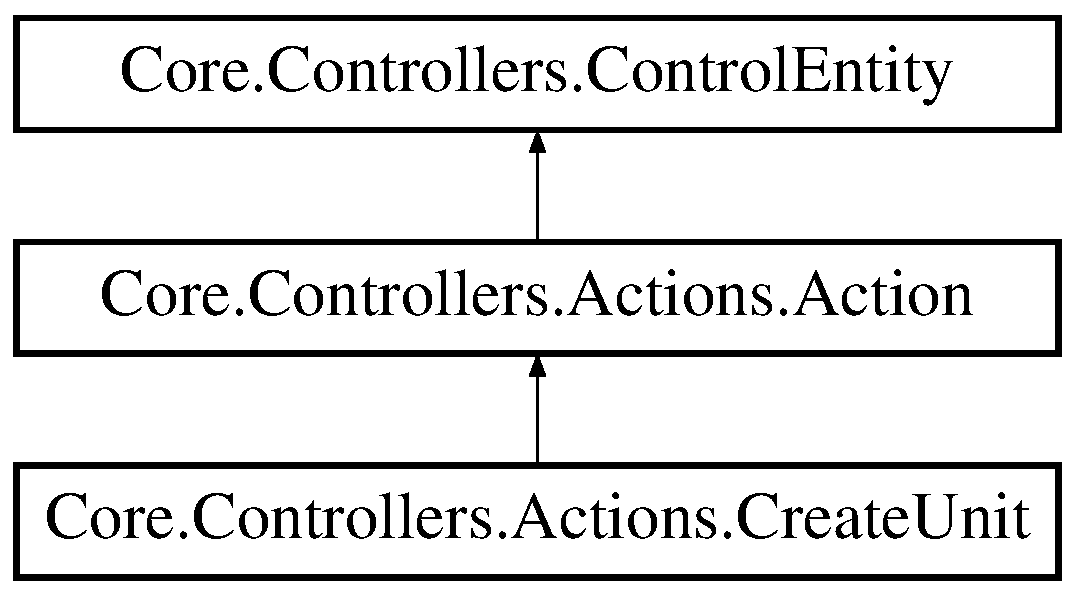
\includegraphics[height=3.000000cm]{classCore_1_1Controllers_1_1Actions_1_1CreateUnit}
\end{center}
\end{figure}
\subsection*{Public Member Functions}
\begin{DoxyCompactItemize}
\item 
\hyperlink{classCore_1_1Controllers_1_1Actions_1_1CreateUnit_a38e1f619d2ec42c361d1ab532b04b2cb}{Create\-Unit} (\hyperlink{classCore_1_1Models_1_1ModelEntity}{Core.\-Models.\-Model\-Entity} model)
\begin{DoxyCompactList}\small\item\em Constructor of the class \hyperlink{classCore_1_1Controllers_1_1Actions_1_1CreateUnit}{Create\-Unit}. \end{DoxyCompactList}\item 
override Concurrent\-Bag\\*
$<$ \hyperlink{classCore_1_1Models_1_1Region}{Core.\-Models.\-Region} $>$ \hyperlink{classCore_1_1Controllers_1_1Actions_1_1CreateUnit_a740be9051fcd4f9a8e22d702da400ba7}{Get\-Affected\-Regions} ()
\begin{DoxyCompactList}\small\item\em /// \end{DoxyCompactList}\item 
override bool \hyperlink{classCore_1_1Controllers_1_1Actions_1_1CreateUnit_a30ceafb2aa0fb1b801a8abd659c9d70f}{Possible} ()
\begin{DoxyCompactList}\small\item\em Returns if the action is even possible. \end{DoxyCompactList}\item 
override Concurrent\-Bag\\*
$<$ \hyperlink{classCore_1_1Models_1_1Region}{Core.\-Models.\-Region} $>$ \hyperlink{classCore_1_1Controllers_1_1Actions_1_1CreateUnit_a0afdf65e7e04f108bb257eae3327eac0}{Do} ()
\begin{DoxyCompactList}\small\item\em Apply action-\/related changes to the world. \end{DoxyCompactList}\item 
override bool \hyperlink{classCore_1_1Controllers_1_1Actions_1_1CreateUnit_ac2763a79e6767ac7c5179281cb4e0a6f}{Catch} ()
\begin{DoxyCompactList}\small\item\em In case of errors, revert the world data to a valid state. \end{DoxyCompactList}\item 
override \hyperlink{classCore_1_1Models_1_1RegionPosition}{Core.\-Models.\-Region\-Position} \hyperlink{classCore_1_1Controllers_1_1Actions_1_1CreateUnit_a04a85d0db9c84ca3f0e97049cca4f9c0}{Get\-Region\-Position} ()
\begin{DoxyCompactList}\small\item\em Gets the region position. \end{DoxyCompactList}\end{DoxyCompactItemize}
\subsection*{Public Attributes}
\begin{DoxyCompactItemize}
\item 
\hypertarget{classCore_1_1Controllers_1_1Actions_1_1CreateUnit_a35a30a8393a155c7bb8e76ecc8c08874}{const string {\bfseries C\-R\-E\-A\-T\-E\-\_\-\-P\-O\-S\-I\-T\-I\-O\-N} = \char`\"{}Create\-Position\char`\"{}}\label{classCore_1_1Controllers_1_1Actions_1_1CreateUnit_a35a30a8393a155c7bb8e76ecc8c08874}

\item 
\hypertarget{classCore_1_1Controllers_1_1Actions_1_1CreateUnit_a2df09d9a45946983c9d5d0ee08a0b4a3}{const string {\bfseries C\-R\-E\-A\-T\-I\-O\-N\-\_\-\-T\-Y\-P\-E} = \char`\"{}Create\-Unit\char`\"{}}\label{classCore_1_1Controllers_1_1Actions_1_1CreateUnit_a2df09d9a45946983c9d5d0ee08a0b4a3}

\item 
\hypertarget{classCore_1_1Controllers_1_1Actions_1_1CreateUnit_a75330207d1027fb83f97d8973ae355f3}{\hyperlink{classCore_1_1Models_1_1PositionI}{Position\-I} {\bfseries Real\-Create\-Position}}\label{classCore_1_1Controllers_1_1Actions_1_1CreateUnit_a75330207d1027fb83f97d8973ae355f3}

\end{DoxyCompactItemize}
\subsection*{Additional Inherited Members}


\subsection{Constructor \& Destructor Documentation}
\hypertarget{classCore_1_1Controllers_1_1Actions_1_1CreateUnit_a38e1f619d2ec42c361d1ab532b04b2cb}{\index{Core\-::\-Controllers\-::\-Actions\-::\-Create\-Unit@{Core\-::\-Controllers\-::\-Actions\-::\-Create\-Unit}!Create\-Unit@{Create\-Unit}}
\index{Create\-Unit@{Create\-Unit}!Core::Controllers::Actions::CreateUnit@{Core\-::\-Controllers\-::\-Actions\-::\-Create\-Unit}}
\subsubsection[{Create\-Unit}]{\setlength{\rightskip}{0pt plus 5cm}Core.\-Controllers.\-Actions.\-Create\-Unit.\-Create\-Unit (
\begin{DoxyParamCaption}
\item[{{\bf Core.\-Models.\-Model\-Entity}}]{model}
\end{DoxyParamCaption}
)\hspace{0.3cm}{\ttfamily [inline]}}}\label{classCore_1_1Controllers_1_1Actions_1_1CreateUnit_a38e1f619d2ec42c361d1ab532b04b2cb}


Constructor of the class \hyperlink{classCore_1_1Controllers_1_1Actions_1_1CreateUnit}{Create\-Unit}. 


\begin{DoxyParams}{Parameters}
{\em model} & \\
\hline
\end{DoxyParams}


\subsection{Member Function Documentation}
\hypertarget{classCore_1_1Controllers_1_1Actions_1_1CreateUnit_ac2763a79e6767ac7c5179281cb4e0a6f}{\index{Core\-::\-Controllers\-::\-Actions\-::\-Create\-Unit@{Core\-::\-Controllers\-::\-Actions\-::\-Create\-Unit}!Catch@{Catch}}
\index{Catch@{Catch}!Core::Controllers::Actions::CreateUnit@{Core\-::\-Controllers\-::\-Actions\-::\-Create\-Unit}}
\subsubsection[{Catch}]{\setlength{\rightskip}{0pt plus 5cm}override bool Core.\-Controllers.\-Actions.\-Create\-Unit.\-Catch (
\begin{DoxyParamCaption}
{}
\end{DoxyParamCaption}
)\hspace{0.3cm}{\ttfamily [inline]}, {\ttfamily [virtual]}}}\label{classCore_1_1Controllers_1_1Actions_1_1CreateUnit_ac2763a79e6767ac7c5179281cb4e0a6f}


In case of errors, revert the world data to a valid state. 



Reimplemented from \hyperlink{classCore_1_1Controllers_1_1Actions_1_1Action_ada4c77dfeee78ded10a6eb6a506defb4}{Core.\-Controllers.\-Actions.\-Action}.

\hypertarget{classCore_1_1Controllers_1_1Actions_1_1CreateUnit_a0afdf65e7e04f108bb257eae3327eac0}{\index{Core\-::\-Controllers\-::\-Actions\-::\-Create\-Unit@{Core\-::\-Controllers\-::\-Actions\-::\-Create\-Unit}!Do@{Do}}
\index{Do@{Do}!Core::Controllers::Actions::CreateUnit@{Core\-::\-Controllers\-::\-Actions\-::\-Create\-Unit}}
\subsubsection[{Do}]{\setlength{\rightskip}{0pt plus 5cm}override Concurrent\-Bag$<${\bf Core.\-Models.\-Region}$>$ Core.\-Controllers.\-Actions.\-Create\-Unit.\-Do (
\begin{DoxyParamCaption}
{}
\end{DoxyParamCaption}
)\hspace{0.3cm}{\ttfamily [inline]}, {\ttfamily [virtual]}}}\label{classCore_1_1Controllers_1_1Actions_1_1CreateUnit_a0afdf65e7e04f108bb257eae3327eac0}


Apply action-\/related changes to the world. 


\begin{DoxyParams}{Parameters}
{\em region\-Manager\-C} & \\
\hline
\end{DoxyParams}
\begin{DoxyReturn}{Returns}
Returns System.\-Collections.\-Concurrent.\-Concurrent\-Bag$<$t$>$ class with the affected region.
\end{DoxyReturn}


Reimplemented from \hyperlink{classCore_1_1Controllers_1_1Actions_1_1Action_afbb091ee28eee896951fac600188d446}{Core.\-Controllers.\-Actions.\-Action}.

\hypertarget{classCore_1_1Controllers_1_1Actions_1_1CreateUnit_a740be9051fcd4f9a8e22d702da400ba7}{\index{Core\-::\-Controllers\-::\-Actions\-::\-Create\-Unit@{Core\-::\-Controllers\-::\-Actions\-::\-Create\-Unit}!Get\-Affected\-Regions@{Get\-Affected\-Regions}}
\index{Get\-Affected\-Regions@{Get\-Affected\-Regions}!Core::Controllers::Actions::CreateUnit@{Core\-::\-Controllers\-::\-Actions\-::\-Create\-Unit}}
\subsubsection[{Get\-Affected\-Regions}]{\setlength{\rightskip}{0pt plus 5cm}override Concurrent\-Bag$<${\bf Core.\-Models.\-Region}$>$ Core.\-Controllers.\-Actions.\-Create\-Unit.\-Get\-Affected\-Regions (
\begin{DoxyParamCaption}
{}
\end{DoxyParamCaption}
)\hspace{0.3cm}{\ttfamily [inline]}, {\ttfamily [virtual]}}}\label{classCore_1_1Controllers_1_1Actions_1_1CreateUnit_a740be9051fcd4f9a8e22d702da400ba7}


/// 

Initializes a new instance of the base.\-control.\-action.\-Action class. Identify alle affected regions by this action. 


\begin{DoxyParams}{Parameters}
{\em region\-Manager\-C} & \\
\hline
\end{DoxyParams}
\begin{DoxyReturn}{Returns}
Returns System.\-Collections.\-Concurrent.\-Concurrent\-Bag$<$t$>$ class with the affected regions. 
\end{DoxyReturn}


Reimplemented from \hyperlink{classCore_1_1Controllers_1_1Actions_1_1Action_aa11bdeffff43ec47ac7c3d6843a85674}{Core.\-Controllers.\-Actions.\-Action}.

\hypertarget{classCore_1_1Controllers_1_1Actions_1_1CreateUnit_a04a85d0db9c84ca3f0e97049cca4f9c0}{\index{Core\-::\-Controllers\-::\-Actions\-::\-Create\-Unit@{Core\-::\-Controllers\-::\-Actions\-::\-Create\-Unit}!Get\-Region\-Position@{Get\-Region\-Position}}
\index{Get\-Region\-Position@{Get\-Region\-Position}!Core::Controllers::Actions::CreateUnit@{Core\-::\-Controllers\-::\-Actions\-::\-Create\-Unit}}
\subsubsection[{Get\-Region\-Position}]{\setlength{\rightskip}{0pt plus 5cm}override {\bf Core.\-Models.\-Region\-Position} Core.\-Controllers.\-Actions.\-Create\-Unit.\-Get\-Region\-Position (
\begin{DoxyParamCaption}
{}
\end{DoxyParamCaption}
)\hspace{0.3cm}{\ttfamily [inline]}, {\ttfamily [virtual]}}}\label{classCore_1_1Controllers_1_1Actions_1_1CreateUnit_a04a85d0db9c84ca3f0e97049cca4f9c0}


Gets the region position. 

\begin{DoxyReturn}{Returns}
The region position.
\end{DoxyReturn}


Reimplemented from \hyperlink{classCore_1_1Controllers_1_1Actions_1_1Action_a6ffe3c30cb5648a81f50096f4f332d5a}{Core.\-Controllers.\-Actions.\-Action}.

\hypertarget{classCore_1_1Controllers_1_1Actions_1_1CreateUnit_a30ceafb2aa0fb1b801a8abd659c9d70f}{\index{Core\-::\-Controllers\-::\-Actions\-::\-Create\-Unit@{Core\-::\-Controllers\-::\-Actions\-::\-Create\-Unit}!Possible@{Possible}}
\index{Possible@{Possible}!Core::Controllers::Actions::CreateUnit@{Core\-::\-Controllers\-::\-Actions\-::\-Create\-Unit}}
\subsubsection[{Possible}]{\setlength{\rightskip}{0pt plus 5cm}override bool Core.\-Controllers.\-Actions.\-Create\-Unit.\-Possible (
\begin{DoxyParamCaption}
{}
\end{DoxyParamCaption}
)\hspace{0.3cm}{\ttfamily [inline]}, {\ttfamily [virtual]}}}\label{classCore_1_1Controllers_1_1Actions_1_1CreateUnit_a30ceafb2aa0fb1b801a8abd659c9d70f}


Returns if the action is even possible. 


\begin{DoxyParams}{Parameters}
{\em region\-Manager\-C} & \\
\hline
\end{DoxyParams}
\begin{DoxyReturn}{Returns}
True if the actions is possible, otherwise false.
\end{DoxyReturn}


Reimplemented from \hyperlink{classCore_1_1Controllers_1_1Actions_1_1Action_a405b995343a9394ad19e05a699a4e6d9}{Core.\-Controllers.\-Actions.\-Action}.



The documentation for this class was generated from the following file\-:\begin{DoxyCompactItemize}
\item 
base/\-Controllers/\-Action/Create\-Unit.\-cs\end{DoxyCompactItemize}

\hypertarget{classCore_1_1Models_1_1Region_1_1DatedActions}{\section{Core.\-Models.\-Region.\-Dated\-Actions Class Reference}
\label{classCore_1_1Models_1_1Region_1_1DatedActions}\index{Core.\-Models.\-Region.\-Dated\-Actions@{Core.\-Models.\-Region.\-Dated\-Actions}}
}
\subsection*{Public Attributes}
\begin{DoxyCompactItemize}
\item 
\hypertarget{classCore_1_1Models_1_1Region_1_1DatedActions_aacd25bcefeefe28cab23509157ceafbf}{Date\-Time {\bfseries Date\-Time}}\label{classCore_1_1Models_1_1Region_1_1DatedActions_aacd25bcefeefe28cab23509157ceafbf}

\item 
\hypertarget{classCore_1_1Models_1_1Region_1_1DatedActions_aeaa886f5b32791bbd8d3a98b9712c1e1}{Linked\-List$<$ \hyperlink{classCore_1_1Models_1_1Action}{Core.\-Models.\-Action} $>$ {\bfseries Actions}}\label{classCore_1_1Models_1_1Region_1_1DatedActions_aeaa886f5b32791bbd8d3a98b9712c1e1}

\item 
\hypertarget{classCore_1_1Models_1_1Region_1_1DatedActions_af5d142eb58d87b6d923f221b18b3bb20}{\hyperlink{classCore_1_1Models_1_1RegionPosition}{Region\-Position} {\bfseries Region\-Position}}\label{classCore_1_1Models_1_1Region_1_1DatedActions_af5d142eb58d87b6d923f221b18b3bb20}

\end{DoxyCompactItemize}


The documentation for this class was generated from the following file\-:\begin{DoxyCompactItemize}
\item 
base/\-Models/\-Map/Region.\-cs\end{DoxyCompactItemize}

\hypertarget{classCore_1_1Models_1_1Region_1_1DatedEntities}{}\section{Core.\+Models.\+Region.\+Dated\+Entities Class Reference}
\label{classCore_1_1Models_1_1Region_1_1DatedEntities}\index{Core.\+Models.\+Region.\+Dated\+Entities@{Core.\+Models.\+Region.\+Dated\+Entities}}


Entities and an date when the last entity was changed  


\subsection*{Public Attributes}
\begin{DoxyCompactItemize}
\item 
Date\+Time \hyperlink{classCore_1_1Models_1_1Region_1_1DatedEntities_aef27626e67d6fbe5e549f57bf1233571}{Date\+Time}
\begin{DoxyCompactList}\small\item\em The last date time when an entity was changed. \end{DoxyCompactList}\item 
Linked\+List$<$ \hyperlink{classCore_1_1Models_1_1Entity}{Entity} $>$ \hyperlink{classCore_1_1Models_1_1Region_1_1DatedEntities_aaa8cacb9e8c527149f8176ad2b473bdc}{Entities}
\begin{DoxyCompactList}\small\item\em The entities. \end{DoxyCompactList}\item 
\hyperlink{classCore_1_1Models_1_1RegionPosition}{Region\+Position} \hyperlink{classCore_1_1Models_1_1Region_1_1DatedEntities_a9f7508c71a4e63dd41df20a6699c4359}{Region\+Position}
\begin{DoxyCompactList}\small\item\em \hyperlink{classCore_1_1Models_1_1RegionPosition}{Region\+Position} of the region which contains the entities \end{DoxyCompactList}\end{DoxyCompactItemize}


\subsection{Detailed Description}
Entities and an date when the last entity was changed 



\subsection{Member Data Documentation}
\hypertarget{classCore_1_1Models_1_1Region_1_1DatedEntities_aef27626e67d6fbe5e549f57bf1233571}{}\index{Core\+::\+Models\+::\+Region\+::\+Dated\+Entities@{Core\+::\+Models\+::\+Region\+::\+Dated\+Entities}!Date\+Time@{Date\+Time}}
\index{Date\+Time@{Date\+Time}!Core\+::\+Models\+::\+Region\+::\+Dated\+Entities@{Core\+::\+Models\+::\+Region\+::\+Dated\+Entities}}
\subsubsection[{Date\+Time}]{\setlength{\rightskip}{0pt plus 5cm}Date\+Time Core.\+Models.\+Region.\+Dated\+Entities.\+Date\+Time}\label{classCore_1_1Models_1_1Region_1_1DatedEntities_aef27626e67d6fbe5e549f57bf1233571}


The last date time when an entity was changed. 

\hypertarget{classCore_1_1Models_1_1Region_1_1DatedEntities_aaa8cacb9e8c527149f8176ad2b473bdc}{}\index{Core\+::\+Models\+::\+Region\+::\+Dated\+Entities@{Core\+::\+Models\+::\+Region\+::\+Dated\+Entities}!Entities@{Entities}}
\index{Entities@{Entities}!Core\+::\+Models\+::\+Region\+::\+Dated\+Entities@{Core\+::\+Models\+::\+Region\+::\+Dated\+Entities}}
\subsubsection[{Entities}]{\setlength{\rightskip}{0pt plus 5cm}Linked\+List$<${\bf Entity}$>$ Core.\+Models.\+Region.\+Dated\+Entities.\+Entities}\label{classCore_1_1Models_1_1Region_1_1DatedEntities_aaa8cacb9e8c527149f8176ad2b473bdc}


The entities. 

\hypertarget{classCore_1_1Models_1_1Region_1_1DatedEntities_a9f7508c71a4e63dd41df20a6699c4359}{}\index{Core\+::\+Models\+::\+Region\+::\+Dated\+Entities@{Core\+::\+Models\+::\+Region\+::\+Dated\+Entities}!Region\+Position@{Region\+Position}}
\index{Region\+Position@{Region\+Position}!Core\+::\+Models\+::\+Region\+::\+Dated\+Entities@{Core\+::\+Models\+::\+Region\+::\+Dated\+Entities}}
\subsubsection[{Region\+Position}]{\setlength{\rightskip}{0pt plus 5cm}{\bf Region\+Position} Core.\+Models.\+Region.\+Dated\+Entities.\+Region\+Position}\label{classCore_1_1Models_1_1Region_1_1DatedEntities_a9f7508c71a4e63dd41df20a6699c4359}


\hyperlink{classCore_1_1Models_1_1RegionPosition}{Region\+Position} of the region which contains the entities 



The documentation for this class was generated from the following file\+:\begin{DoxyCompactItemize}
\item 
base/\+Models/\+Map/Region.\+cs\end{DoxyCompactItemize}

\hypertarget{classServer_1_1DB_1_1DBAccount}{\section{Server.\-D\-B.\-D\-B\-Account Class Reference}
\label{classServer_1_1DB_1_1DBAccount}\index{Server.\-D\-B.\-D\-B\-Account@{Server.\-D\-B.\-D\-B\-Account}}
}


\hyperlink{namespaceServer_1_1DB}{D\-B} account.  


\subsection*{Public Member Functions}
\begin{DoxyCompactItemize}
\item 
\hyperlink{classServer_1_1DB_1_1DBAccount_a09329b7a7cc362eca6d1d54571159395}{D\-B\-Account} (\hyperlink{classSQLite_1_1SQLiteConnection}{S\-Q\-Lite\-Connection} con)
\begin{DoxyCompactList}\small\item\em Initializes a new instance of the server.\-D\-B.\-D\-B\-Account class. \end{DoxyCompactList}\item 
void \hyperlink{classServer_1_1DB_1_1DBAccount_a3b7e2921efb6f6e7ceecba07d3068a1f}{Create\-Account} (\hyperlink{classCore_1_1Models_1_1Account}{Account} account, string password)
\begin{DoxyCompactList}\small\item\em Creates the account with username, password, and the calculated salt value. \end{DoxyCompactList}\item 
bool \hyperlink{classServer_1_1DB_1_1DBAccount_a53bbc0085fc15347e5d67ff1ee9ee925}{Login} (string username, string password)
\begin{DoxyCompactList}\small\item\em Login the specified username and password. \end{DoxyCompactList}\end{DoxyCompactItemize}


\subsection{Detailed Description}
\hyperlink{namespaceServer_1_1DB}{D\-B} account. 



\subsection{Constructor \& Destructor Documentation}
\hypertarget{classServer_1_1DB_1_1DBAccount_a09329b7a7cc362eca6d1d54571159395}{\index{Server\-::\-D\-B\-::\-D\-B\-Account@{Server\-::\-D\-B\-::\-D\-B\-Account}!D\-B\-Account@{D\-B\-Account}}
\index{D\-B\-Account@{D\-B\-Account}!Server::DB::DBAccount@{Server\-::\-D\-B\-::\-D\-B\-Account}}
\subsubsection[{D\-B\-Account}]{\setlength{\rightskip}{0pt plus 5cm}Server.\-D\-B.\-D\-B\-Account.\-D\-B\-Account (
\begin{DoxyParamCaption}
\item[{{\bf S\-Q\-Lite\-Connection}}]{con}
\end{DoxyParamCaption}
)\hspace{0.3cm}{\ttfamily [inline]}}}\label{classServer_1_1DB_1_1DBAccount_a09329b7a7cc362eca6d1d54571159395}


Initializes a new instance of the server.\-D\-B.\-D\-B\-Account class. 


\begin{DoxyParams}{Parameters}
{\em con} & Connection to the databank.\\
\hline
\end{DoxyParams}


\subsection{Member Function Documentation}
\hypertarget{classServer_1_1DB_1_1DBAccount_a3b7e2921efb6f6e7ceecba07d3068a1f}{\index{Server\-::\-D\-B\-::\-D\-B\-Account@{Server\-::\-D\-B\-::\-D\-B\-Account}!Create\-Account@{Create\-Account}}
\index{Create\-Account@{Create\-Account}!Server::DB::DBAccount@{Server\-::\-D\-B\-::\-D\-B\-Account}}
\subsubsection[{Create\-Account}]{\setlength{\rightskip}{0pt plus 5cm}void Server.\-D\-B.\-D\-B\-Account.\-Create\-Account (
\begin{DoxyParamCaption}
\item[{{\bf Account}}]{account, }
\item[{string}]{password}
\end{DoxyParamCaption}
)\hspace{0.3cm}{\ttfamily [inline]}}}\label{classServer_1_1DB_1_1DBAccount_a3b7e2921efb6f6e7ceecba07d3068a1f}


Creates the account with username, password, and the calculated salt value. 


\begin{DoxyParams}{Parameters}
{\em account} & Account.\\
\hline
{\em password} & Password.\\
\hline
\end{DoxyParams}
\hypertarget{classServer_1_1DB_1_1DBAccount_a53bbc0085fc15347e5d67ff1ee9ee925}{\index{Server\-::\-D\-B\-::\-D\-B\-Account@{Server\-::\-D\-B\-::\-D\-B\-Account}!Login@{Login}}
\index{Login@{Login}!Server::DB::DBAccount@{Server\-::\-D\-B\-::\-D\-B\-Account}}
\subsubsection[{Login}]{\setlength{\rightskip}{0pt plus 5cm}bool Server.\-D\-B.\-D\-B\-Account.\-Login (
\begin{DoxyParamCaption}
\item[{string}]{username, }
\item[{string}]{password}
\end{DoxyParamCaption}
)\hspace{0.3cm}{\ttfamily [inline]}}}\label{classServer_1_1DB_1_1DBAccount_a53bbc0085fc15347e5d67ff1ee9ee925}


Login the specified username and password. 


\begin{DoxyParams}{Parameters}
{\em username} & Username.\\
\hline
{\em password} & Password.\\
\hline
\end{DoxyParams}


The documentation for this class was generated from the following file\-:\begin{DoxyCompactItemize}
\item 
server/\-D\-B/D\-B\-Account.\-cs\end{DoxyCompactItemize}

\hypertarget{classServer_1_1DB_1_1DBBuildings}{\section{Server.\-D\-B.\-D\-B\-Buildings Class Reference}
\label{classServer_1_1DB_1_1DBBuildings}\index{Server.\-D\-B.\-D\-B\-Buildings@{Server.\-D\-B.\-D\-B\-Buildings}}
}


\hyperlink{namespaceServer_1_1DB}{D\-B} buildings.  


\subsection*{Public Member Functions}
\begin{DoxyCompactItemize}
\item 
\hyperlink{classServer_1_1DB_1_1DBBuildings_a077d835984df76dc1810b84223f17c07}{D\-B\-Buildings} (\hyperlink{classSQLite_1_1SQLiteConnection}{S\-Q\-Lite\-Connection} con)
\begin{DoxyCompactList}\small\item\em Initializes a new instance of the server.\-D\-B.\-D\-B\-Buildings class. \end{DoxyCompactList}\item 
void \hyperlink{classServer_1_1DB_1_1DBBuildings_aa0535b132cd346ceef7fa9115e3dcd76}{New\-Buildings} (\hyperlink{classCore_1_1Models_1_1Entity}{Entity} building\-Entity, int id)
\begin{DoxyCompactList}\small\item\em Insert a building into the database, with the current position. \end{DoxyCompactList}\end{DoxyCompactItemize}


\subsection{Detailed Description}
\hyperlink{namespaceServer_1_1DB}{D\-B} buildings. 



\subsection{Constructor \& Destructor Documentation}
\hypertarget{classServer_1_1DB_1_1DBBuildings_a077d835984df76dc1810b84223f17c07}{\index{Server\-::\-D\-B\-::\-D\-B\-Buildings@{Server\-::\-D\-B\-::\-D\-B\-Buildings}!D\-B\-Buildings@{D\-B\-Buildings}}
\index{D\-B\-Buildings@{D\-B\-Buildings}!Server::DB::DBBuildings@{Server\-::\-D\-B\-::\-D\-B\-Buildings}}
\subsubsection[{D\-B\-Buildings}]{\setlength{\rightskip}{0pt plus 5cm}Server.\-D\-B.\-D\-B\-Buildings.\-D\-B\-Buildings (
\begin{DoxyParamCaption}
\item[{{\bf S\-Q\-Lite\-Connection}}]{con}
\end{DoxyParamCaption}
)\hspace{0.3cm}{\ttfamily [inline]}}}\label{classServer_1_1DB_1_1DBBuildings_a077d835984df76dc1810b84223f17c07}


Initializes a new instance of the server.\-D\-B.\-D\-B\-Buildings class. 


\begin{DoxyParams}{Parameters}
{\em con} & Con.\\
\hline
\end{DoxyParams}


\subsection{Member Function Documentation}
\hypertarget{classServer_1_1DB_1_1DBBuildings_aa0535b132cd346ceef7fa9115e3dcd76}{\index{Server\-::\-D\-B\-::\-D\-B\-Buildings@{Server\-::\-D\-B\-::\-D\-B\-Buildings}!New\-Buildings@{New\-Buildings}}
\index{New\-Buildings@{New\-Buildings}!Server::DB::DBBuildings@{Server\-::\-D\-B\-::\-D\-B\-Buildings}}
\subsubsection[{New\-Buildings}]{\setlength{\rightskip}{0pt plus 5cm}void Server.\-D\-B.\-D\-B\-Buildings.\-New\-Buildings (
\begin{DoxyParamCaption}
\item[{{\bf Entity}}]{building\-Entity, }
\item[{int}]{id}
\end{DoxyParamCaption}
)\hspace{0.3cm}{\ttfamily [inline]}}}\label{classServer_1_1DB_1_1DBBuildings_aa0535b132cd346ceef7fa9115e3dcd76}


Insert a building into the database, with the current position. 


\begin{DoxyParams}{Parameters}
{\em building\-Entity} & Building entity.\\
\hline
{\em id} & Identifier.\\
\hline
\end{DoxyParams}


The documentation for this class was generated from the following file\-:\begin{DoxyCompactItemize}
\item 
server/\-D\-B/D\-B\-Buildings.\-cs\end{DoxyCompactItemize}

\hypertarget{classServer_1_1DB_1_1DBHandle}{\section{Server.\-D\-B.\-D\-B\-Handle Class Reference}
\label{classServer_1_1DB_1_1DBHandle}\index{Server.\-D\-B.\-D\-B\-Handle@{Server.\-D\-B.\-D\-B\-Handle}}
}


\hyperlink{namespaceServer_1_1DB}{D\-B} handle.  


\subsection*{Public Member Functions}
\begin{DoxyCompactItemize}
\item 
void \hyperlink{classServer_1_1DB_1_1DBHandle_a81ca48e0929da58ec2ac4b55081d16c8}{Create\-New\-D\-B\-Account} (\hyperlink{classCore_1_1Models_1_1Account}{Account} account, string password)
\begin{DoxyCompactList}\small\item\em Creates the new \hyperlink{namespaceServer_1_1DB}{D\-B} account. \end{DoxyCompactList}\item 
\hyperlink{classServer_1_1DB_1_1Models_1_1TableData}{Table\-Data} \hyperlink{classServer_1_1DB_1_1DBHandle_a3a15cdbe25a8893c41f90b334ae34f66}{Get\-Account\-Data\-Via\-D\-B\-Login} (\hyperlink{classCore_1_1Models_1_1Account}{Account} account, string password)
\begin{DoxyCompactList}\small\item\em Gets the account data via \hyperlink{namespaceServer_1_1DB}{D\-B} login. \end{DoxyCompactList}\item 
\hyperlink{classServer_1_1DB_1_1Models_1_1TableData}{Table\-Data} \hyperlink{classServer_1_1DB_1_1DBHandle_a8f5f08824cea64c884f93494bd55c623}{Get\-Account\-Data\-Via\-I\-D} (int Id)
\begin{DoxyCompactList}\small\item\em Gets the account data via I\-D. \end{DoxyCompactList}\item 
void \hyperlink{classServer_1_1DB_1_1DBHandle_ab381614c199bdf2782df0c69e99edfb4}{Insert\-Into\-Unit} (int id, \hyperlink{classCore_1_1Models_1_1Entity}{Entity} unit\-Entity)
\begin{DoxyCompactList}\small\item\em Inserts the unitv into the databank. \end{DoxyCompactList}\item 
void \hyperlink{classServer_1_1DB_1_1DBHandle_a8fbc59cc6602d140482f68f3477e4baf}{Insert\-Into\-Building} (int id, \hyperlink{classCore_1_1Models_1_1Entity}{Entity} building\-Entity)
\begin{DoxyCompactList}\small\item\em Inserts the building into the databank. \end{DoxyCompactList}\item 
void \hyperlink{classServer_1_1DB_1_1DBHandle_a34b8a21944a12dd60e3f95d49e174458}{Insert\-Into\-Resource} (int ressource\-Fire, int ressource\-Earth, int ressource\-Water, int ressource\-Air, int ressource\-Magic, int ressource\-Gold, int id)
\begin{DoxyCompactList}\small\item\em Inserts the resource into the databank, which belong to the owner Id.. \end{DoxyCompactList}\item 
void \hyperlink{classServer_1_1DB_1_1DBHandle_af9bdbff3aeab46d1632f447f99989557}{Update\-Unit} (\hyperlink{classCore_1_1Models_1_1Entity}{Entity} unit\-Entity, int id)
\begin{DoxyCompactList}\small\item\em Updates the unit, which belong to the owner Id. \end{DoxyCompactList}\item 
void \hyperlink{classServer_1_1DB_1_1DBHandle_aa32ad499307c7d70ff263c9136126aac}{Update\-Building} (\hyperlink{classCore_1_1Models_1_1Entity}{Entity} building\-Entity, int id)
\begin{DoxyCompactList}\small\item\em Updates the building, which belong to the owner Id. \end{DoxyCompactList}\item 
void \hyperlink{classServer_1_1DB_1_1DBHandle_a227b450add1e80fcf329e62b9464b5e6}{Insert\-All\-Units} (I\-List$<$ \hyperlink{classCore_1_1Models_1_1Entity}{Entity} $>$ unit\-Entitiys, int id)
\begin{DoxyCompactList}\small\item\em Inserts all units, which belong to the owner Id. \end{DoxyCompactList}\item 
void \hyperlink{classServer_1_1DB_1_1DBHandle_ab7d27c190063a6cb8c6db0240c7c3dd1}{Insert\-All\-Buildings} (I\-List$<$ \hyperlink{classCore_1_1Models_1_1Entity}{Entity} $>$ building\-Entitys, int id)
\begin{DoxyCompactList}\small\item\em Inserts all buildings, which belong to the owner Id. \end{DoxyCompactList}\item 
void \hyperlink{classServer_1_1DB_1_1DBHandle_a1bd86a76e3ff01f2a378c75dc4cb28d3}{Update\-Ressource} (int ressource\-Fire, int ressource\-Earth, int ressource\-Water, int ressource\-Air, int ressource\-Magic, int ressource\-Gold, int id)
\begin{DoxyCompactList}\small\item\em Updates the ressource, which belong to the owner Id. \end{DoxyCompactList}\item 
void \hyperlink{classServer_1_1DB_1_1DBHandle_a149e5c4a88f7abebe3039ec647c97b00}{Delete\-Unit} (int id)
\begin{DoxyCompactList}\small\item\em Deletes the unit. \end{DoxyCompactList}\item 
void \hyperlink{classServer_1_1DB_1_1DBHandle_a7e3257d50f7e4ae4d2cde720a336711e}{Delete\-Building} (int id)
\begin{DoxyCompactList}\small\item\em Deletes the building. \end{DoxyCompactList}\item 
void \hyperlink{classServer_1_1DB_1_1DBHandle_a6401b9d859f8c7852fd1fb8d08fbcab5}{Delete\-Account\-From\-All\-Tables} (int id)
\begin{DoxyCompactList}\small\item\em Deletes the account from all tables. \end{DoxyCompactList}\end{DoxyCompactItemize}
\subsection*{Properties}
\begin{DoxyCompactItemize}
\item 
static \hyperlink{classServer_1_1DB_1_1DBHandle}{D\-B\-Handle} \hyperlink{classServer_1_1DB_1_1DBHandle_a1809fac85ce06cf9e7f400ac4648051e}{Instance}\hspace{0.3cm}{\ttfamily  \mbox{[}get\mbox{]}}
\begin{DoxyCompactList}\small\item\em Gets the instance. \end{DoxyCompactList}\end{DoxyCompactItemize}


\subsection{Detailed Description}
\hyperlink{namespaceServer_1_1DB}{D\-B} handle. 



\subsection{Member Function Documentation}
\hypertarget{classServer_1_1DB_1_1DBHandle_a81ca48e0929da58ec2ac4b55081d16c8}{\index{Server\-::\-D\-B\-::\-D\-B\-Handle@{Server\-::\-D\-B\-::\-D\-B\-Handle}!Create\-New\-D\-B\-Account@{Create\-New\-D\-B\-Account}}
\index{Create\-New\-D\-B\-Account@{Create\-New\-D\-B\-Account}!Server::DB::DBHandle@{Server\-::\-D\-B\-::\-D\-B\-Handle}}
\subsubsection[{Create\-New\-D\-B\-Account}]{\setlength{\rightskip}{0pt plus 5cm}void Server.\-D\-B.\-D\-B\-Handle.\-Create\-New\-D\-B\-Account (
\begin{DoxyParamCaption}
\item[{{\bf Account}}]{account, }
\item[{string}]{password}
\end{DoxyParamCaption}
)\hspace{0.3cm}{\ttfamily [inline]}}}\label{classServer_1_1DB_1_1DBHandle_a81ca48e0929da58ec2ac4b55081d16c8}


Creates the new \hyperlink{namespaceServer_1_1DB}{D\-B} account. 


\begin{DoxyParams}{Parameters}
{\em account} & Account.\\
\hline
{\em password} & Password.\\
\hline
\end{DoxyParams}
\hypertarget{classServer_1_1DB_1_1DBHandle_a6401b9d859f8c7852fd1fb8d08fbcab5}{\index{Server\-::\-D\-B\-::\-D\-B\-Handle@{Server\-::\-D\-B\-::\-D\-B\-Handle}!Delete\-Account\-From\-All\-Tables@{Delete\-Account\-From\-All\-Tables}}
\index{Delete\-Account\-From\-All\-Tables@{Delete\-Account\-From\-All\-Tables}!Server::DB::DBHandle@{Server\-::\-D\-B\-::\-D\-B\-Handle}}
\subsubsection[{Delete\-Account\-From\-All\-Tables}]{\setlength{\rightskip}{0pt plus 5cm}void Server.\-D\-B.\-D\-B\-Handle.\-Delete\-Account\-From\-All\-Tables (
\begin{DoxyParamCaption}
\item[{int}]{id}
\end{DoxyParamCaption}
)\hspace{0.3cm}{\ttfamily [inline]}}}\label{classServer_1_1DB_1_1DBHandle_a6401b9d859f8c7852fd1fb8d08fbcab5}


Deletes the account from all tables. 


\begin{DoxyParams}{Parameters}
{\em id} & Identifier.\\
\hline
\end{DoxyParams}
\hypertarget{classServer_1_1DB_1_1DBHandle_a7e3257d50f7e4ae4d2cde720a336711e}{\index{Server\-::\-D\-B\-::\-D\-B\-Handle@{Server\-::\-D\-B\-::\-D\-B\-Handle}!Delete\-Building@{Delete\-Building}}
\index{Delete\-Building@{Delete\-Building}!Server::DB::DBHandle@{Server\-::\-D\-B\-::\-D\-B\-Handle}}
\subsubsection[{Delete\-Building}]{\setlength{\rightskip}{0pt plus 5cm}void Server.\-D\-B.\-D\-B\-Handle.\-Delete\-Building (
\begin{DoxyParamCaption}
\item[{int}]{id}
\end{DoxyParamCaption}
)\hspace{0.3cm}{\ttfamily [inline]}}}\label{classServer_1_1DB_1_1DBHandle_a7e3257d50f7e4ae4d2cde720a336711e}


Deletes the building. 


\begin{DoxyParams}{Parameters}
{\em id} & Identifier.\\
\hline
\end{DoxyParams}
\hypertarget{classServer_1_1DB_1_1DBHandle_a149e5c4a88f7abebe3039ec647c97b00}{\index{Server\-::\-D\-B\-::\-D\-B\-Handle@{Server\-::\-D\-B\-::\-D\-B\-Handle}!Delete\-Unit@{Delete\-Unit}}
\index{Delete\-Unit@{Delete\-Unit}!Server::DB::DBHandle@{Server\-::\-D\-B\-::\-D\-B\-Handle}}
\subsubsection[{Delete\-Unit}]{\setlength{\rightskip}{0pt plus 5cm}void Server.\-D\-B.\-D\-B\-Handle.\-Delete\-Unit (
\begin{DoxyParamCaption}
\item[{int}]{id}
\end{DoxyParamCaption}
)\hspace{0.3cm}{\ttfamily [inline]}}}\label{classServer_1_1DB_1_1DBHandle_a149e5c4a88f7abebe3039ec647c97b00}


Deletes the unit. 


\begin{DoxyParams}{Parameters}
{\em id} & Identifier.\\
\hline
\end{DoxyParams}
\hypertarget{classServer_1_1DB_1_1DBHandle_a3a15cdbe25a8893c41f90b334ae34f66}{\index{Server\-::\-D\-B\-::\-D\-B\-Handle@{Server\-::\-D\-B\-::\-D\-B\-Handle}!Get\-Account\-Data\-Via\-D\-B\-Login@{Get\-Account\-Data\-Via\-D\-B\-Login}}
\index{Get\-Account\-Data\-Via\-D\-B\-Login@{Get\-Account\-Data\-Via\-D\-B\-Login}!Server::DB::DBHandle@{Server\-::\-D\-B\-::\-D\-B\-Handle}}
\subsubsection[{Get\-Account\-Data\-Via\-D\-B\-Login}]{\setlength{\rightskip}{0pt plus 5cm}{\bf Table\-Data} Server.\-D\-B.\-D\-B\-Handle.\-Get\-Account\-Data\-Via\-D\-B\-Login (
\begin{DoxyParamCaption}
\item[{{\bf Account}}]{account, }
\item[{string}]{password}
\end{DoxyParamCaption}
)\hspace{0.3cm}{\ttfamily [inline]}}}\label{classServer_1_1DB_1_1DBHandle_a3a15cdbe25a8893c41f90b334ae34f66}


Gets the account data via \hyperlink{namespaceServer_1_1DB}{D\-B} login. 

\begin{DoxyReturn}{Returns}
The account data via \hyperlink{namespaceServer_1_1DB}{D\-B} login.
\end{DoxyReturn}

\begin{DoxyParams}{Parameters}
{\em account} & Account.\\
\hline
{\em password} & Password.\\
\hline
\end{DoxyParams}
\hypertarget{classServer_1_1DB_1_1DBHandle_a8f5f08824cea64c884f93494bd55c623}{\index{Server\-::\-D\-B\-::\-D\-B\-Handle@{Server\-::\-D\-B\-::\-D\-B\-Handle}!Get\-Account\-Data\-Via\-I\-D@{Get\-Account\-Data\-Via\-I\-D}}
\index{Get\-Account\-Data\-Via\-I\-D@{Get\-Account\-Data\-Via\-I\-D}!Server::DB::DBHandle@{Server\-::\-D\-B\-::\-D\-B\-Handle}}
\subsubsection[{Get\-Account\-Data\-Via\-I\-D}]{\setlength{\rightskip}{0pt plus 5cm}{\bf Table\-Data} Server.\-D\-B.\-D\-B\-Handle.\-Get\-Account\-Data\-Via\-I\-D (
\begin{DoxyParamCaption}
\item[{int}]{Id}
\end{DoxyParamCaption}
)\hspace{0.3cm}{\ttfamily [inline]}}}\label{classServer_1_1DB_1_1DBHandle_a8f5f08824cea64c884f93494bd55c623}


Gets the account data via I\-D. 

\begin{DoxyReturn}{Returns}
The account data via I\-D.
\end{DoxyReturn}

\begin{DoxyParams}{Parameters}
{\em Id} & Identifier.\\
\hline
\end{DoxyParams}
\hypertarget{classServer_1_1DB_1_1DBHandle_ab7d27c190063a6cb8c6db0240c7c3dd1}{\index{Server\-::\-D\-B\-::\-D\-B\-Handle@{Server\-::\-D\-B\-::\-D\-B\-Handle}!Insert\-All\-Buildings@{Insert\-All\-Buildings}}
\index{Insert\-All\-Buildings@{Insert\-All\-Buildings}!Server::DB::DBHandle@{Server\-::\-D\-B\-::\-D\-B\-Handle}}
\subsubsection[{Insert\-All\-Buildings}]{\setlength{\rightskip}{0pt plus 5cm}void Server.\-D\-B.\-D\-B\-Handle.\-Insert\-All\-Buildings (
\begin{DoxyParamCaption}
\item[{I\-List$<$ {\bf Entity} $>$}]{building\-Entitys, }
\item[{int}]{id}
\end{DoxyParamCaption}
)\hspace{0.3cm}{\ttfamily [inline]}}}\label{classServer_1_1DB_1_1DBHandle_ab7d27c190063a6cb8c6db0240c7c3dd1}


Inserts all buildings, which belong to the owner Id. 


\begin{DoxyParams}{Parameters}
{\em building\-Entitys} & Building entitys.\\
\hline
{\em id} & Identifier.\\
\hline
\end{DoxyParams}
\hypertarget{classServer_1_1DB_1_1DBHandle_a227b450add1e80fcf329e62b9464b5e6}{\index{Server\-::\-D\-B\-::\-D\-B\-Handle@{Server\-::\-D\-B\-::\-D\-B\-Handle}!Insert\-All\-Units@{Insert\-All\-Units}}
\index{Insert\-All\-Units@{Insert\-All\-Units}!Server::DB::DBHandle@{Server\-::\-D\-B\-::\-D\-B\-Handle}}
\subsubsection[{Insert\-All\-Units}]{\setlength{\rightskip}{0pt plus 5cm}void Server.\-D\-B.\-D\-B\-Handle.\-Insert\-All\-Units (
\begin{DoxyParamCaption}
\item[{I\-List$<$ {\bf Entity} $>$}]{unit\-Entitiys, }
\item[{int}]{id}
\end{DoxyParamCaption}
)\hspace{0.3cm}{\ttfamily [inline]}}}\label{classServer_1_1DB_1_1DBHandle_a227b450add1e80fcf329e62b9464b5e6}


Inserts all units, which belong to the owner Id. 


\begin{DoxyParams}{Parameters}
{\em unit\-Entitiys} & Unit entitiys.\\
\hline
{\em id} & Identifier.\\
\hline
\end{DoxyParams}
\hypertarget{classServer_1_1DB_1_1DBHandle_a8fbc59cc6602d140482f68f3477e4baf}{\index{Server\-::\-D\-B\-::\-D\-B\-Handle@{Server\-::\-D\-B\-::\-D\-B\-Handle}!Insert\-Into\-Building@{Insert\-Into\-Building}}
\index{Insert\-Into\-Building@{Insert\-Into\-Building}!Server::DB::DBHandle@{Server\-::\-D\-B\-::\-D\-B\-Handle}}
\subsubsection[{Insert\-Into\-Building}]{\setlength{\rightskip}{0pt plus 5cm}void Server.\-D\-B.\-D\-B\-Handle.\-Insert\-Into\-Building (
\begin{DoxyParamCaption}
\item[{int}]{id, }
\item[{{\bf Entity}}]{building\-Entity}
\end{DoxyParamCaption}
)\hspace{0.3cm}{\ttfamily [inline]}}}\label{classServer_1_1DB_1_1DBHandle_a8fbc59cc6602d140482f68f3477e4baf}


Inserts the building into the databank. 


\begin{DoxyParams}{Parameters}
{\em id} & Identifier.\\
\hline
{\em building\-Entity} & Building entity.\\
\hline
\end{DoxyParams}
\hypertarget{classServer_1_1DB_1_1DBHandle_a34b8a21944a12dd60e3f95d49e174458}{\index{Server\-::\-D\-B\-::\-D\-B\-Handle@{Server\-::\-D\-B\-::\-D\-B\-Handle}!Insert\-Into\-Resource@{Insert\-Into\-Resource}}
\index{Insert\-Into\-Resource@{Insert\-Into\-Resource}!Server::DB::DBHandle@{Server\-::\-D\-B\-::\-D\-B\-Handle}}
\subsubsection[{Insert\-Into\-Resource}]{\setlength{\rightskip}{0pt plus 5cm}void Server.\-D\-B.\-D\-B\-Handle.\-Insert\-Into\-Resource (
\begin{DoxyParamCaption}
\item[{int}]{ressource\-Fire, }
\item[{int}]{ressource\-Earth, }
\item[{int}]{ressource\-Water, }
\item[{int}]{ressource\-Air, }
\item[{int}]{ressource\-Magic, }
\item[{int}]{ressource\-Gold, }
\item[{int}]{id}
\end{DoxyParamCaption}
)\hspace{0.3cm}{\ttfamily [inline]}}}\label{classServer_1_1DB_1_1DBHandle_a34b8a21944a12dd60e3f95d49e174458}


Inserts the resource into the databank, which belong to the owner Id.. 


\begin{DoxyParams}{Parameters}
{\em ressource\-Fire} & Ressource fire.\\
\hline
{\em ressource\-Earth} & Ressource earth.\\
\hline
{\em ressource\-Water} & Ressource water.\\
\hline
{\em ressource\-Air} & Ressource air.\\
\hline
{\em ressource\-Magic} & Ressource magic.\\
\hline
{\em ressource\-Gold} & Ressource gold.\\
\hline
{\em id} & Identifier.\\
\hline
\end{DoxyParams}
\hypertarget{classServer_1_1DB_1_1DBHandle_ab381614c199bdf2782df0c69e99edfb4}{\index{Server\-::\-D\-B\-::\-D\-B\-Handle@{Server\-::\-D\-B\-::\-D\-B\-Handle}!Insert\-Into\-Unit@{Insert\-Into\-Unit}}
\index{Insert\-Into\-Unit@{Insert\-Into\-Unit}!Server::DB::DBHandle@{Server\-::\-D\-B\-::\-D\-B\-Handle}}
\subsubsection[{Insert\-Into\-Unit}]{\setlength{\rightskip}{0pt plus 5cm}void Server.\-D\-B.\-D\-B\-Handle.\-Insert\-Into\-Unit (
\begin{DoxyParamCaption}
\item[{int}]{id, }
\item[{{\bf Entity}}]{unit\-Entity}
\end{DoxyParamCaption}
)\hspace{0.3cm}{\ttfamily [inline]}}}\label{classServer_1_1DB_1_1DBHandle_ab381614c199bdf2782df0c69e99edfb4}


Inserts the unitv into the databank. 


\begin{DoxyParams}{Parameters}
{\em id} & Identifier.\\
\hline
{\em unit\-Entity} & Unit entity.\\
\hline
\end{DoxyParams}
\hypertarget{classServer_1_1DB_1_1DBHandle_aa32ad499307c7d70ff263c9136126aac}{\index{Server\-::\-D\-B\-::\-D\-B\-Handle@{Server\-::\-D\-B\-::\-D\-B\-Handle}!Update\-Building@{Update\-Building}}
\index{Update\-Building@{Update\-Building}!Server::DB::DBHandle@{Server\-::\-D\-B\-::\-D\-B\-Handle}}
\subsubsection[{Update\-Building}]{\setlength{\rightskip}{0pt plus 5cm}void Server.\-D\-B.\-D\-B\-Handle.\-Update\-Building (
\begin{DoxyParamCaption}
\item[{{\bf Entity}}]{building\-Entity, }
\item[{int}]{id}
\end{DoxyParamCaption}
)\hspace{0.3cm}{\ttfamily [inline]}}}\label{classServer_1_1DB_1_1DBHandle_aa32ad499307c7d70ff263c9136126aac}


Updates the building, which belong to the owner Id. 


\begin{DoxyParams}{Parameters}
{\em building\-Entity} & Building entity.\\
\hline
{\em id} & Identifier.\\
\hline
\end{DoxyParams}
\hypertarget{classServer_1_1DB_1_1DBHandle_a1bd86a76e3ff01f2a378c75dc4cb28d3}{\index{Server\-::\-D\-B\-::\-D\-B\-Handle@{Server\-::\-D\-B\-::\-D\-B\-Handle}!Update\-Ressource@{Update\-Ressource}}
\index{Update\-Ressource@{Update\-Ressource}!Server::DB::DBHandle@{Server\-::\-D\-B\-::\-D\-B\-Handle}}
\subsubsection[{Update\-Ressource}]{\setlength{\rightskip}{0pt plus 5cm}void Server.\-D\-B.\-D\-B\-Handle.\-Update\-Ressource (
\begin{DoxyParamCaption}
\item[{int}]{ressource\-Fire, }
\item[{int}]{ressource\-Earth, }
\item[{int}]{ressource\-Water, }
\item[{int}]{ressource\-Air, }
\item[{int}]{ressource\-Magic, }
\item[{int}]{ressource\-Gold, }
\item[{int}]{id}
\end{DoxyParamCaption}
)\hspace{0.3cm}{\ttfamily [inline]}}}\label{classServer_1_1DB_1_1DBHandle_a1bd86a76e3ff01f2a378c75dc4cb28d3}


Updates the ressource, which belong to the owner Id. 


\begin{DoxyParams}{Parameters}
{\em ressource\-Fire} & Ressource fire.\\
\hline
{\em ressource\-Earth} & Ressource earth.\\
\hline
{\em ressource\-Water} & Ressource water.\\
\hline
{\em ressource\-Air} & Ressource air.\\
\hline
{\em ressource\-Magic} & Ressource magic.\\
\hline
{\em ressource\-Gold} & Ressource gold.\\
\hline
{\em id} & Identifier.\\
\hline
\end{DoxyParams}
\hypertarget{classServer_1_1DB_1_1DBHandle_af9bdbff3aeab46d1632f447f99989557}{\index{Server\-::\-D\-B\-::\-D\-B\-Handle@{Server\-::\-D\-B\-::\-D\-B\-Handle}!Update\-Unit@{Update\-Unit}}
\index{Update\-Unit@{Update\-Unit}!Server::DB::DBHandle@{Server\-::\-D\-B\-::\-D\-B\-Handle}}
\subsubsection[{Update\-Unit}]{\setlength{\rightskip}{0pt plus 5cm}void Server.\-D\-B.\-D\-B\-Handle.\-Update\-Unit (
\begin{DoxyParamCaption}
\item[{{\bf Entity}}]{unit\-Entity, }
\item[{int}]{id}
\end{DoxyParamCaption}
)\hspace{0.3cm}{\ttfamily [inline]}}}\label{classServer_1_1DB_1_1DBHandle_af9bdbff3aeab46d1632f447f99989557}


Updates the unit, which belong to the owner Id. 


\begin{DoxyParams}{Parameters}
{\em unit\-Entity} & Unit entity.\\
\hline
{\em id} & Identifier.\\
\hline
\end{DoxyParams}


\subsection{Property Documentation}
\hypertarget{classServer_1_1DB_1_1DBHandle_a1809fac85ce06cf9e7f400ac4648051e}{\index{Server\-::\-D\-B\-::\-D\-B\-Handle@{Server\-::\-D\-B\-::\-D\-B\-Handle}!Instance@{Instance}}
\index{Instance@{Instance}!Server::DB::DBHandle@{Server\-::\-D\-B\-::\-D\-B\-Handle}}
\subsubsection[{Instance}]{\setlength{\rightskip}{0pt plus 5cm}{\bf D\-B\-Handle} Server.\-D\-B.\-D\-B\-Handle.\-Instance\hspace{0.3cm}{\ttfamily [static]}, {\ttfamily [get]}}}\label{classServer_1_1DB_1_1DBHandle_a1809fac85ce06cf9e7f400ac4648051e}


Gets the instance. 

The instance.

The documentation for this class was generated from the following file\-:\begin{DoxyCompactItemize}
\item 
server/\-D\-B/D\-B\-Handle.\-cs\end{DoxyCompactItemize}

\hypertarget{classserver_1_1DB_1_1DBLogin}{\section{server.\-D\-B.\-D\-B\-Login Class Reference}
\label{classserver_1_1DB_1_1DBLogin}\index{server.\-D\-B.\-D\-B\-Login@{server.\-D\-B.\-D\-B\-Login}}
}
\subsection*{Public Member Functions}
\begin{DoxyCompactItemize}
\item 
\hypertarget{classserver_1_1DB_1_1DBLogin_a1fdcdcbdefddfaaeadcda4f3ba068995}{void {\bfseries Table\-Account} (Account account, string password)}\label{classserver_1_1DB_1_1DBLogin_a1fdcdcbdefddfaaeadcda4f3ba068995}

\end{DoxyCompactItemize}


The documentation for this class was generated from the following file\-:\begin{DoxyCompactItemize}
\item 
server/\-D\-B/D\-B\-Login.\-cs\end{DoxyCompactItemize}

\hypertarget{classServer_1_1DB_1_1DBRessource}{\section{Server.\-D\-B.\-D\-B\-Ressource Class Reference}
\label{classServer_1_1DB_1_1DBRessource}\index{Server.\-D\-B.\-D\-B\-Ressource@{Server.\-D\-B.\-D\-B\-Ressource}}
}


\hyperlink{namespaceServer_1_1DB}{D\-B} ressource.  


\subsection*{Public Member Functions}
\begin{DoxyCompactItemize}
\item 
\hyperlink{classServer_1_1DB_1_1DBRessource_ad3ae43c5661467a23be8b40386fde94f}{D\-B\-Ressource} (\hyperlink{classSQLite_1_1SQLiteConnection}{S\-Q\-Lite\-Connection} con)
\begin{DoxyCompactList}\small\item\em Initializes a new instance of the server.\-D\-B.\-D\-B\-Ressource class. \end{DoxyCompactList}\item 
void \hyperlink{classServer_1_1DB_1_1DBRessource_a7a0e9627e0ebde571a3211defbf86111}{Table\-Ressource} (int ressource\-Fire, int ressource\-Earth, int ressource\-Water, int ressource\-Air, int ressource\-Magic, int ressource\-Gold, int id)
\begin{DoxyCompactList}\small\item\em Insert all ressources into the databank. \end{DoxyCompactList}\end{DoxyCompactItemize}


\subsection{Detailed Description}
\hyperlink{namespaceServer_1_1DB}{D\-B} ressource. 



\subsection{Constructor \& Destructor Documentation}
\hypertarget{classServer_1_1DB_1_1DBRessource_ad3ae43c5661467a23be8b40386fde94f}{\index{Server\-::\-D\-B\-::\-D\-B\-Ressource@{Server\-::\-D\-B\-::\-D\-B\-Ressource}!D\-B\-Ressource@{D\-B\-Ressource}}
\index{D\-B\-Ressource@{D\-B\-Ressource}!Server::DB::DBRessource@{Server\-::\-D\-B\-::\-D\-B\-Ressource}}
\subsubsection[{D\-B\-Ressource}]{\setlength{\rightskip}{0pt plus 5cm}Server.\-D\-B.\-D\-B\-Ressource.\-D\-B\-Ressource (
\begin{DoxyParamCaption}
\item[{{\bf S\-Q\-Lite\-Connection}}]{con}
\end{DoxyParamCaption}
)\hspace{0.3cm}{\ttfamily [inline]}}}\label{classServer_1_1DB_1_1DBRessource_ad3ae43c5661467a23be8b40386fde94f}


Initializes a new instance of the server.\-D\-B.\-D\-B\-Ressource class. 


\begin{DoxyParams}{Parameters}
{\em con} & Con.\\
\hline
\end{DoxyParams}


\subsection{Member Function Documentation}
\hypertarget{classServer_1_1DB_1_1DBRessource_a7a0e9627e0ebde571a3211defbf86111}{\index{Server\-::\-D\-B\-::\-D\-B\-Ressource@{Server\-::\-D\-B\-::\-D\-B\-Ressource}!Table\-Ressource@{Table\-Ressource}}
\index{Table\-Ressource@{Table\-Ressource}!Server::DB::DBRessource@{Server\-::\-D\-B\-::\-D\-B\-Ressource}}
\subsubsection[{Table\-Ressource}]{\setlength{\rightskip}{0pt plus 5cm}void Server.\-D\-B.\-D\-B\-Ressource.\-Table\-Ressource (
\begin{DoxyParamCaption}
\item[{int}]{ressource\-Fire, }
\item[{int}]{ressource\-Earth, }
\item[{int}]{ressource\-Water, }
\item[{int}]{ressource\-Air, }
\item[{int}]{ressource\-Magic, }
\item[{int}]{ressource\-Gold, }
\item[{int}]{id}
\end{DoxyParamCaption}
)\hspace{0.3cm}{\ttfamily [inline]}}}\label{classServer_1_1DB_1_1DBRessource_a7a0e9627e0ebde571a3211defbf86111}


Insert all ressources into the databank. 


\begin{DoxyParams}{Parameters}
{\em ressource\-Fire} & Ressource fire.\\
\hline
{\em ressource\-Earth} & Ressource earth.\\
\hline
{\em ressource\-Water} & Ressource water.\\
\hline
{\em ressource\-Air} & Ressource air.\\
\hline
{\em ressource\-Magic} & Ressource magic.\\
\hline
{\em ressource\-Gold} & Ressource gold.\\
\hline
{\em id} & Identifier.\\
\hline
\end{DoxyParams}


The documentation for this class was generated from the following file\-:\begin{DoxyCompactItemize}
\item 
server/\-D\-B/D\-B\-Ressource.\-cs\end{DoxyCompactItemize}

\hypertarget{classServer_1_1DB_1_1DBUnits}{\section{Server.\-D\-B.\-D\-B\-Units Class Reference}
\label{classServer_1_1DB_1_1DBUnits}\index{Server.\-D\-B.\-D\-B\-Units@{Server.\-D\-B.\-D\-B\-Units}}
}


\hyperlink{namespaceServer_1_1DB}{D\-B} units.  


\subsection*{Public Member Functions}
\begin{DoxyCompactItemize}
\item 
\hyperlink{classServer_1_1DB_1_1DBUnits_a5f007f724ddf2a3fe727238515435926}{D\-B\-Units} (\hyperlink{classSQLite_1_1SQLiteConnection}{S\-Q\-Lite\-Connection} con)
\begin{DoxyCompactList}\small\item\em Initializes a new instance of the server.\-D\-B.\-D\-B\-Units class. \end{DoxyCompactList}\item 
void \hyperlink{classServer_1_1DB_1_1DBUnits_a37696a3723e722005d922ef4ac5272ea}{New\-Unit} (\hyperlink{classCore_1_1Models_1_1Entity}{Entity} unit\-Entity, int id)
\begin{DoxyCompactList}\small\item\em Insert a new unit into the databank. \end{DoxyCompactList}\end{DoxyCompactItemize}


\subsection{Detailed Description}
\hyperlink{namespaceServer_1_1DB}{D\-B} units. 



\subsection{Constructor \& Destructor Documentation}
\hypertarget{classServer_1_1DB_1_1DBUnits_a5f007f724ddf2a3fe727238515435926}{\index{Server\-::\-D\-B\-::\-D\-B\-Units@{Server\-::\-D\-B\-::\-D\-B\-Units}!D\-B\-Units@{D\-B\-Units}}
\index{D\-B\-Units@{D\-B\-Units}!Server::DB::DBUnits@{Server\-::\-D\-B\-::\-D\-B\-Units}}
\subsubsection[{D\-B\-Units}]{\setlength{\rightskip}{0pt plus 5cm}Server.\-D\-B.\-D\-B\-Units.\-D\-B\-Units (
\begin{DoxyParamCaption}
\item[{{\bf S\-Q\-Lite\-Connection}}]{con}
\end{DoxyParamCaption}
)\hspace{0.3cm}{\ttfamily [inline]}}}\label{classServer_1_1DB_1_1DBUnits_a5f007f724ddf2a3fe727238515435926}


Initializes a new instance of the server.\-D\-B.\-D\-B\-Units class. 


\begin{DoxyParams}{Parameters}
{\em con} & Con.\\
\hline
\end{DoxyParams}


\subsection{Member Function Documentation}
\hypertarget{classServer_1_1DB_1_1DBUnits_a37696a3723e722005d922ef4ac5272ea}{\index{Server\-::\-D\-B\-::\-D\-B\-Units@{Server\-::\-D\-B\-::\-D\-B\-Units}!New\-Unit@{New\-Unit}}
\index{New\-Unit@{New\-Unit}!Server::DB::DBUnits@{Server\-::\-D\-B\-::\-D\-B\-Units}}
\subsubsection[{New\-Unit}]{\setlength{\rightskip}{0pt plus 5cm}void Server.\-D\-B.\-D\-B\-Units.\-New\-Unit (
\begin{DoxyParamCaption}
\item[{{\bf Entity}}]{unit\-Entity, }
\item[{int}]{id}
\end{DoxyParamCaption}
)\hspace{0.3cm}{\ttfamily [inline]}}}\label{classServer_1_1DB_1_1DBUnits_a37696a3723e722005d922ef4ac5272ea}


Insert a new unit into the databank. 


\begin{DoxyParams}{Parameters}
{\em unit\-Entity} & Unit entity.\\
\hline
{\em id} & Identifier.\\
\hline
\end{DoxyParams}


The documentation for this class was generated from the following file\-:\begin{DoxyCompactItemize}
\item 
server/\-D\-B/D\-B\-Units.\-cs\end{DoxyCompactItemize}

\hypertarget{classCore_1_1Models_1_1Definitions_1_1Definition}{\section{Core.\-Models.\-Definitions.\-Definition Class Reference}
\label{classCore_1_1Models_1_1Definitions_1_1Definition}\index{Core.\-Models.\-Definitions.\-Definition@{Core.\-Models.\-Definitions.\-Definition}}
}


\hyperlink{classCore_1_1Models_1_1Definitions_1_1Definition}{Definition} contains static informations about entities. In which Category they belong and their id. Will be used as base-\/class for other definitions.  


Inheritance diagram for Core.\-Models.\-Definitions.\-Definition\-:\begin{figure}[H]
\begin{center}
\leavevmode
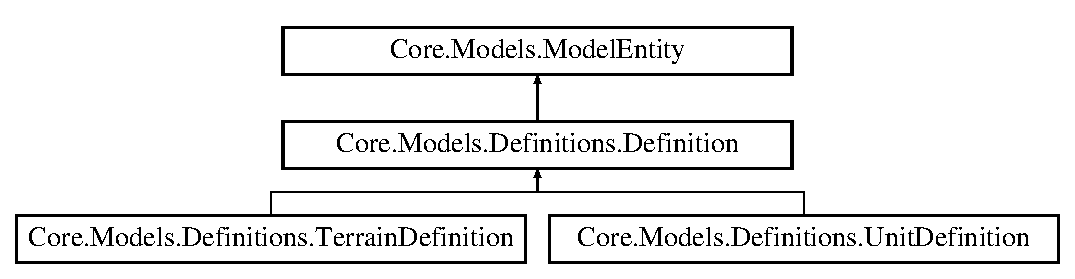
\includegraphics[height=2.000000cm]{classCore_1_1Models_1_1Definitions_1_1Definition}
\end{center}
\end{figure}
\subsection*{Public Member Functions}
\begin{DoxyCompactItemize}
\item 
\hypertarget{classCore_1_1Models_1_1Definitions_1_1Definition_a58b73a00c59e999041dffb2b6a273d8f}{{\bfseries Definition} (int id)}\label{classCore_1_1Models_1_1Definitions_1_1Definition_a58b73a00c59e999041dffb2b6a273d8f}

\end{DoxyCompactItemize}
\subsection*{Properties}
\begin{DoxyCompactItemize}
\item 
\hypertarget{classCore_1_1Models_1_1Definitions_1_1Definition_a6504fe4404e24c0b0601b0591f99fda4}{int {\bfseries I\-D}\hspace{0.3cm}{\ttfamily  \mbox{[}get, set\mbox{]}}}\label{classCore_1_1Models_1_1Definitions_1_1Definition_a6504fe4404e24c0b0601b0591f99fda4}

\item 
\hypertarget{classCore_1_1Models_1_1Definitions_1_1Definition_abbcf001ffb2d8453d321e3524739b48e}{\hyperlink{namespaceCore_1_1Models_1_1Definitions_a8be0403c3e883fe583d7bb3893c22c65}{Category} {\bfseries Category}\hspace{0.3cm}{\ttfamily  \mbox{[}get\mbox{]}}}\label{classCore_1_1Models_1_1Definitions_1_1Definition_abbcf001ffb2d8453d321e3524739b48e}

\item 
\hypertarget{classCore_1_1Models_1_1Definitions_1_1Definition_ae71f596d97485f31733d1b9b5144051a}{\hyperlink{namespaceCore_1_1Models_1_1Definitions_a609ed13db028308ebc6c5fbd98615fdc}{Entity\-Type} {\bfseries Sub\-Type}\hspace{0.3cm}{\ttfamily  \mbox{[}get\mbox{]}}}\label{classCore_1_1Models_1_1Definitions_1_1Definition_ae71f596d97485f31733d1b9b5144051a}

\end{DoxyCompactItemize}


\subsection{Detailed Description}
\hyperlink{classCore_1_1Models_1_1Definitions_1_1Definition}{Definition} contains static informations about entities. In which Category they belong and their id. Will be used as base-\/class for other definitions. 



The documentation for this class was generated from the following file\-:\begin{DoxyCompactItemize}
\item 
base/\-Models/\-Definitions/Definition.\-cs\end{DoxyCompactItemize}

\hypertarget{classCore_1_1Models_1_1DefinitionManager}{\section{Core.\-Models.\-Definition\-Manager Class Reference}
\label{classCore_1_1Models_1_1DefinitionManager}\index{Core.\-Models.\-Definition\-Manager@{Core.\-Models.\-Definition\-Manager}}
}


Contains all \hyperlink{namespaceCore_1_1Models_1_1Definitions}{Definitions}.  


\subsection*{Public Member Functions}
\begin{DoxyCompactItemize}
\item 
\hypertarget{classCore_1_1Models_1_1DefinitionManager_a08d79c044487af124f2a449e200e84c2}{\hyperlink{classCore_1_1Models_1_1Definitions_1_1Definition}{Definition} {\bfseries Get\-Definition} (\hyperlink{namespaceCore_1_1Models_1_1Definitions_a609ed13db028308ebc6c5fbd98615fdc}{Entity\-Type} entity\-Type)}\label{classCore_1_1Models_1_1DefinitionManager_a08d79c044487af124f2a449e200e84c2}

\item 
\hypertarget{classCore_1_1Models_1_1DefinitionManager_a11c894ac62397f0ecd223475f81ac770}{void {\bfseries Add\-Definition} (\hyperlink{classCore_1_1Models_1_1Definitions_1_1Definition}{Definition} definition)}\label{classCore_1_1Models_1_1DefinitionManager_a11c894ac62397f0ecd223475f81ac770}

\end{DoxyCompactItemize}


\subsection{Detailed Description}
Contains all \hyperlink{namespaceCore_1_1Models_1_1Definitions}{Definitions}. 



The documentation for this class was generated from the following file\-:\begin{DoxyCompactItemize}
\item 
base/\-Models/\-Manager/Definition\-Manager.\-cs\end{DoxyCompactItemize}

\hypertarget{classCore_1_1Controllers_1_1DefinitionManagerController}{\section{Core.\-Controllers.\-Definition\-Manager\-Controller Class Reference}
\label{classCore_1_1Controllers_1_1DefinitionManagerController}\index{Core.\-Controllers.\-Definition\-Manager\-Controller@{Core.\-Controllers.\-Definition\-Manager\-Controller}}
}
Inheritance diagram for Core.\-Controllers.\-Definition\-Manager\-Controller\-:\begin{figure}[H]
\begin{center}
\leavevmode
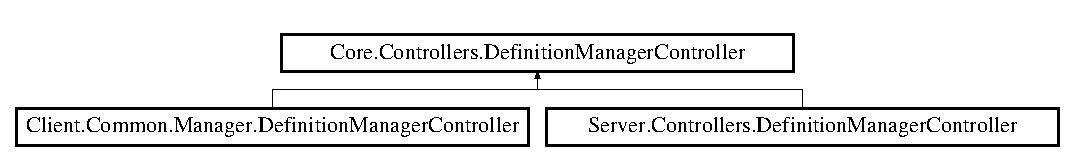
\includegraphics[height=1.733746cm]{classCore_1_1Controllers_1_1DefinitionManagerController}
\end{center}
\end{figure}
\subsection*{Properties}
\begin{DoxyCompactItemize}
\item 
\hypertarget{classCore_1_1Controllers_1_1DefinitionManagerController_ada4b684abad134fa15ed076dccb20a89}{\hyperlink{classCore_1_1Models_1_1DefinitionManager}{Definition\-Manager} {\bfseries Definition\-Manager}\hspace{0.3cm}{\ttfamily  \mbox{[}get\mbox{]}}}\label{classCore_1_1Controllers_1_1DefinitionManagerController_ada4b684abad134fa15ed076dccb20a89}

\end{DoxyCompactItemize}


The documentation for this class was generated from the following file\-:\begin{DoxyCompactItemize}
\item 
base/\-Controllers/Definition\-Manager\-Controller.\-cs\end{DoxyCompactItemize}

\hypertarget{classClient_1_1Common_1_1Manager_1_1DefinitionManagerController}{\section{Client.\-Common.\-Manager.\-Definition\-Manager\-Controller Class Reference}
\label{classClient_1_1Common_1_1Manager_1_1DefinitionManagerController}\index{Client.\-Common.\-Manager.\-Definition\-Manager\-Controller@{Client.\-Common.\-Manager.\-Definition\-Manager\-Controller}}
}


Definition manager controller laod definitions and fill the definition manager  


Inheritance diagram for Client.\-Common.\-Manager.\-Definition\-Manager\-Controller\-:\begin{figure}[H]
\begin{center}
\leavevmode
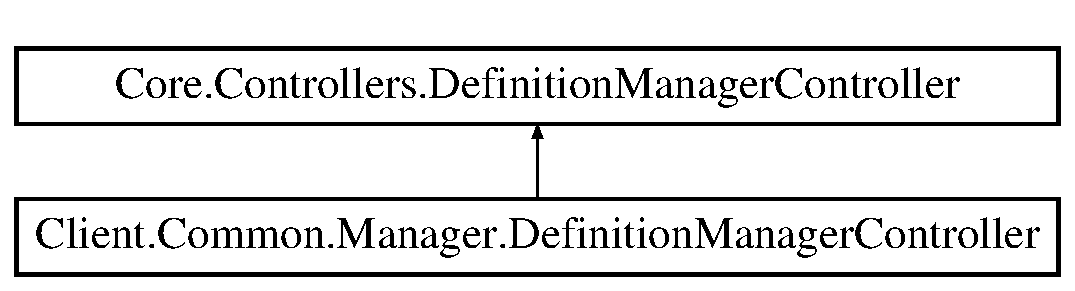
\includegraphics[height=2.000000cm]{classClient_1_1Common_1_1Manager_1_1DefinitionManagerController}
\end{center}
\end{figure}
\subsection*{Public Member Functions}
\begin{DoxyCompactItemize}
\item 
\hyperlink{classClient_1_1Common_1_1Manager_1_1DefinitionManagerController_a96a7c15eea1a7237941000f9008ab808}{Definition\-Manager\-Controller} ()
\begin{DoxyCompactList}\small\item\em Initializes a new instance of the client.\-Common.\-Manager.\-Definition\-Manager\-Controller class. \end{DoxyCompactList}\item 
async Task \hyperlink{classClient_1_1Common_1_1Manager_1_1DefinitionManagerController_aa551f263205c884e7e9255a95b3731e9}{Load\-Terrain\-Definitions\-Async} ()
\begin{DoxyCompactList}\small\item\em Loads the terrain definitions async, serialize the definitions and add the definition in to the definition manager. \end{DoxyCompactList}\item 
async Task \hyperlink{classClient_1_1Common_1_1Manager_1_1DefinitionManagerController_a4a20fe19a6a0ce7b3a1525894ddade4b}{Load\-Unit\-Definitions\-Async} ()
\begin{DoxyCompactList}\small\item\em Loads the Unit definitions async, serialize the definitions and add the definition in to the definition manager. \end{DoxyCompactList}\end{DoxyCompactItemize}
\subsection*{Additional Inherited Members}


\subsection{Detailed Description}
Definition manager controller laod definitions and fill the definition manager 



\subsection{Constructor \& Destructor Documentation}
\hypertarget{classClient_1_1Common_1_1Manager_1_1DefinitionManagerController_a96a7c15eea1a7237941000f9008ab808}{\index{Client\-::\-Common\-::\-Manager\-::\-Definition\-Manager\-Controller@{Client\-::\-Common\-::\-Manager\-::\-Definition\-Manager\-Controller}!Definition\-Manager\-Controller@{Definition\-Manager\-Controller}}
\index{Definition\-Manager\-Controller@{Definition\-Manager\-Controller}!Client::Common::Manager::DefinitionManagerController@{Client\-::\-Common\-::\-Manager\-::\-Definition\-Manager\-Controller}}
\subsubsection[{Definition\-Manager\-Controller}]{\setlength{\rightskip}{0pt plus 5cm}Client.\-Common.\-Manager.\-Definition\-Manager\-Controller.\-Definition\-Manager\-Controller (
\begin{DoxyParamCaption}
{}
\end{DoxyParamCaption}
)\hspace{0.3cm}{\ttfamily [inline]}}}\label{classClient_1_1Common_1_1Manager_1_1DefinitionManagerController_a96a7c15eea1a7237941000f9008ab808}


Initializes a new instance of the client.\-Common.\-Manager.\-Definition\-Manager\-Controller class. 



\subsection{Member Function Documentation}
\hypertarget{classClient_1_1Common_1_1Manager_1_1DefinitionManagerController_aa551f263205c884e7e9255a95b3731e9}{\index{Client\-::\-Common\-::\-Manager\-::\-Definition\-Manager\-Controller@{Client\-::\-Common\-::\-Manager\-::\-Definition\-Manager\-Controller}!Load\-Terrain\-Definitions\-Async@{Load\-Terrain\-Definitions\-Async}}
\index{Load\-Terrain\-Definitions\-Async@{Load\-Terrain\-Definitions\-Async}!Client::Common::Manager::DefinitionManagerController@{Client\-::\-Common\-::\-Manager\-::\-Definition\-Manager\-Controller}}
\subsubsection[{Load\-Terrain\-Definitions\-Async}]{\setlength{\rightskip}{0pt plus 5cm}async Task Client.\-Common.\-Manager.\-Definition\-Manager\-Controller.\-Load\-Terrain\-Definitions\-Async (
\begin{DoxyParamCaption}
{}
\end{DoxyParamCaption}
)\hspace{0.3cm}{\ttfamily [inline]}}}\label{classClient_1_1Common_1_1Manager_1_1DefinitionManagerController_aa551f263205c884e7e9255a95b3731e9}


Loads the terrain definitions async, serialize the definitions and add the definition in to the definition manager. 

\hypertarget{classClient_1_1Common_1_1Manager_1_1DefinitionManagerController_a4a20fe19a6a0ce7b3a1525894ddade4b}{\index{Client\-::\-Common\-::\-Manager\-::\-Definition\-Manager\-Controller@{Client\-::\-Common\-::\-Manager\-::\-Definition\-Manager\-Controller}!Load\-Unit\-Definitions\-Async@{Load\-Unit\-Definitions\-Async}}
\index{Load\-Unit\-Definitions\-Async@{Load\-Unit\-Definitions\-Async}!Client::Common::Manager::DefinitionManagerController@{Client\-::\-Common\-::\-Manager\-::\-Definition\-Manager\-Controller}}
\subsubsection[{Load\-Unit\-Definitions\-Async}]{\setlength{\rightskip}{0pt plus 5cm}async Task Client.\-Common.\-Manager.\-Definition\-Manager\-Controller.\-Load\-Unit\-Definitions\-Async (
\begin{DoxyParamCaption}
{}
\end{DoxyParamCaption}
)\hspace{0.3cm}{\ttfamily [inline]}}}\label{classClient_1_1Common_1_1Manager_1_1DefinitionManagerController_a4a20fe19a6a0ce7b3a1525894ddade4b}


Loads the Unit definitions async, serialize the definitions and add the definition in to the definition manager. 



The documentation for this class was generated from the following file\-:\begin{DoxyCompactItemize}
\item 
client/client/client.\-Common/\-Manager/Definition\-Manager\-Controller.\-cs\end{DoxyCompactItemize}

\hypertarget{classServer_1_1Controllers_1_1DefinitionManagerController}{}\section{Server.\+Controllers.\+Definition\+Manager\+Controller Class Reference}
\label{classServer_1_1Controllers_1_1DefinitionManagerController}\index{Server.\+Controllers.\+Definition\+Manager\+Controller@{Server.\+Controllers.\+Definition\+Manager\+Controller}}


Loads the Definitions and contains them.  


Inheritance diagram for Server.\+Controllers.\+Definition\+Manager\+Controller\+:\begin{figure}[H]
\begin{center}
\leavevmode
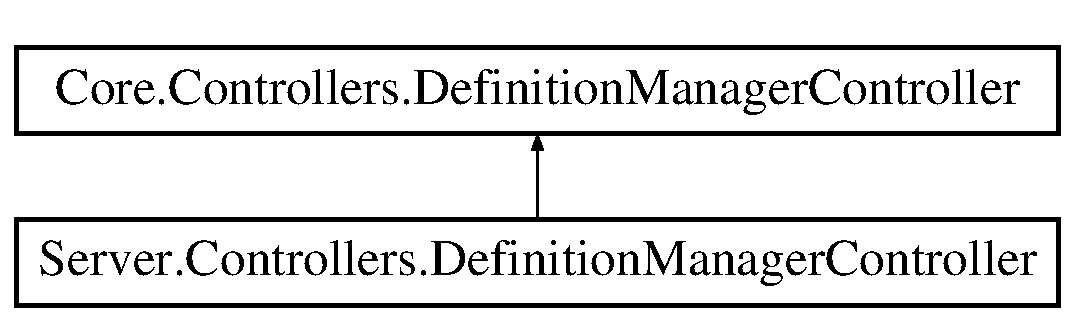
\includegraphics[height=2.000000cm]{classServer_1_1Controllers_1_1DefinitionManagerController}
\end{center}
\end{figure}
\subsection*{Public Member Functions}
\begin{DoxyCompactItemize}
\item 
\hyperlink{classServer_1_1Controllers_1_1DefinitionManagerController_afc57fe6b2fb92f1f45d106e4bd7853b5}{Definition\+Manager\+Controller} ()
\begin{DoxyCompactList}\small\item\em Initializes a new instance of the \hyperlink{classServer_1_1Controllers_1_1DefinitionManagerController}{Server.\+Controllers.\+Definition\+Manager\+Controller} class. \end{DoxyCompactList}\end{DoxyCompactItemize}
\subsection*{Additional Inherited Members}


\subsection{Detailed Description}
Loads the Definitions and contains them. 



\subsection{Constructor \& Destructor Documentation}
\hypertarget{classServer_1_1Controllers_1_1DefinitionManagerController_afc57fe6b2fb92f1f45d106e4bd7853b5}{}\index{Server\+::\+Controllers\+::\+Definition\+Manager\+Controller@{Server\+::\+Controllers\+::\+Definition\+Manager\+Controller}!Definition\+Manager\+Controller@{Definition\+Manager\+Controller}}
\index{Definition\+Manager\+Controller@{Definition\+Manager\+Controller}!Server\+::\+Controllers\+::\+Definition\+Manager\+Controller@{Server\+::\+Controllers\+::\+Definition\+Manager\+Controller}}
\subsubsection[{Definition\+Manager\+Controller()}]{\setlength{\rightskip}{0pt plus 5cm}Server.\+Controllers.\+Definition\+Manager\+Controller.\+Definition\+Manager\+Controller (
\begin{DoxyParamCaption}
{}
\end{DoxyParamCaption}
)}\label{classServer_1_1Controllers_1_1DefinitionManagerController_afc57fe6b2fb92f1f45d106e4bd7853b5}


Initializes a new instance of the \hyperlink{classServer_1_1Controllers_1_1DefinitionManagerController}{Server.\+Controllers.\+Definition\+Manager\+Controller} class. 



The documentation for this class was generated from the following file\+:\begin{DoxyCompactItemize}
\item 
tcpserver/\+Controllers/Definition\+Manager\+Controller.\+cs\end{DoxyCompactItemize}

\hypertarget{classClient_1_1Common_1_1Models_1_1Device}{\section{Client.\-Common.\-Models.\-Device Class Reference}
\label{classClient_1_1Common_1_1Models_1_1Device}\index{Client.\-Common.\-Models.\-Device@{Client.\-Common.\-Models.\-Device}}
}
Inheritance diagram for Client.\-Common.\-Models.\-Device\-:\begin{figure}[H]
\begin{center}
\leavevmode
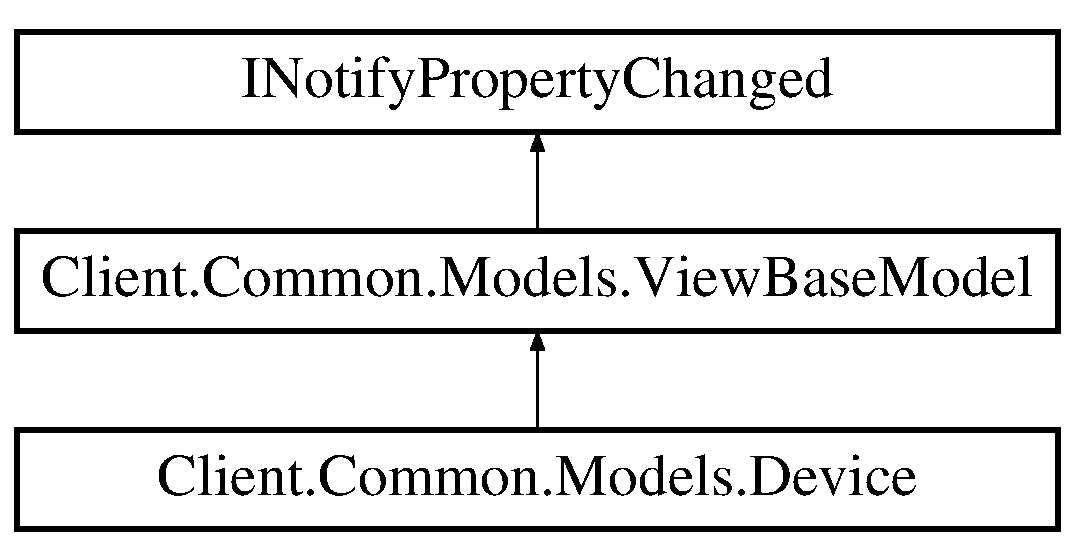
\includegraphics[height=3.000000cm]{classClient_1_1Common_1_1Models_1_1Device}
\end{center}
\end{figure}
\subsection*{Static Public Attributes}
\begin{DoxyCompactItemize}
\item 
\hypertarget{classClient_1_1Common_1_1Models_1_1Device_ac51bdfcd52ea6fcb3ebbc379ecc82829}{static string {\bfseries Property\-Name\-Battery\-Level} = \char`\"{}Battery\-Level\char`\"{}}\label{classClient_1_1Common_1_1Models_1_1Device_ac51bdfcd52ea6fcb3ebbc379ecc82829}

\item 
\hypertarget{classClient_1_1Common_1_1Models_1_1Device_aea7be474dead31b9fcabffdb266f7a03}{static string {\bfseries Property\-Name\-Device\-Id} = \char`\"{}Device\-Id\char`\"{}}\label{classClient_1_1Common_1_1Models_1_1Device_aea7be474dead31b9fcabffdb266f7a03}

\item 
\hypertarget{classClient_1_1Common_1_1Models_1_1Device_ab66cfe6644008ed175969d9dc9276827}{static string {\bfseries Property\-Name\-Firmware\-Version} = \char`\"{}Firmware\-Version\char`\"{}}\label{classClient_1_1Common_1_1Models_1_1Device_ab66cfe6644008ed175969d9dc9276827}

\item 
\hypertarget{classClient_1_1Common_1_1Models_1_1Device_a8fe8d07281f944b0f402859b6da8eb59}{static string {\bfseries Property\-Name\-Hardware\-Version} = \char`\"{}Hardware\-Version\char`\"{}}\label{classClient_1_1Common_1_1Models_1_1Device_a8fe8d07281f944b0f402859b6da8eb59}

\item 
\hypertarget{classClient_1_1Common_1_1Models_1_1Device_a009bb1cd55e95065c37ce793c09d8065}{static string {\bfseries Property\-Name\-Language\-Code} = \char`\"{}Language\-Code\char`\"{}}\label{classClient_1_1Common_1_1Models_1_1Device_a009bb1cd55e95065c37ce793c09d8065}

\item 
\hypertarget{classClient_1_1Common_1_1Models_1_1Device_abdd5f3df306c43e6a9a36616d60ff66a}{static string {\bfseries Property\-Name\-Manufacturer} = \char`\"{}Manufacturer\char`\"{}}\label{classClient_1_1Common_1_1Models_1_1Device_abdd5f3df306c43e6a9a36616d60ff66a}

\item 
\hypertarget{classClient_1_1Common_1_1Models_1_1Device_a92eaec1dc6ba592a7b7c9fc66b71c2bc}{static string {\bfseries Property\-Name\-Device\-Name} = \char`\"{}Device\-Name\char`\"{}}\label{classClient_1_1Common_1_1Models_1_1Device_a92eaec1dc6ba592a7b7c9fc66b71c2bc}

\item 
\hypertarget{classClient_1_1Common_1_1Models_1_1Device_a343a8a0276f050dcb42f439b750df14d}{static string {\bfseries Property\-Name\-Time\-Zone} = \char`\"{}Time\-Zone\char`\"{}}\label{classClient_1_1Common_1_1Models_1_1Device_a343a8a0276f050dcb42f439b750df14d}

\item 
\hypertarget{classClient_1_1Common_1_1Models_1_1Device_a15d2f2a780082f7623b582c806f8d095}{static string {\bfseries Property\-Name\-Time\-Zone\-Offset} = \char`\"{}Time\-Zone\-Offset\char`\"{}}\label{classClient_1_1Common_1_1Models_1_1Device_a15d2f2a780082f7623b582c806f8d095}

\item 
\hypertarget{classClient_1_1Common_1_1Models_1_1Device_ad6116529786054397d7a73c806a66c66}{static string {\bfseries Property\-Name\-Device\-Memory} = \char`\"{}Device\-Memory\char`\"{}}\label{classClient_1_1Common_1_1Models_1_1Device_ad6116529786054397d7a73c806a66c66}

\end{DoxyCompactItemize}
\subsection*{Properties}
\begin{DoxyCompactItemize}
\item 
\hypertarget{classClient_1_1Common_1_1Models_1_1Device_a7fad57259329dad5815137c963961689}{static \hyperlink{classClient_1_1Common_1_1Models_1_1Device}{Device} {\bfseries Get\-Instance}\hspace{0.3cm}{\ttfamily  \mbox{[}get\mbox{]}}}\label{classClient_1_1Common_1_1Models_1_1Device_a7fad57259329dad5815137c963961689}

\item 
\hypertarget{classClient_1_1Common_1_1Models_1_1Device_a850d4b4655dfaa9ce9467ba84a9d01c7}{I\-Accelerometer {\bfseries Accelerometer}\hspace{0.3cm}{\ttfamily  \mbox{[}get, set\mbox{]}}}\label{classClient_1_1Common_1_1Models_1_1Device_a850d4b4655dfaa9ce9467ba84a9d01c7}

\item 
\hypertarget{classClient_1_1Common_1_1Models_1_1Device_a8c719b6d0548aabbbf37a811267ffc8e}{I\-Battery {\bfseries Battery}\hspace{0.3cm}{\ttfamily  \mbox{[}get, set\mbox{]}}}\label{classClient_1_1Common_1_1Models_1_1Device_a8c719b6d0548aabbbf37a811267ffc8e}

\item 
\hypertarget{classClient_1_1Common_1_1Models_1_1Device_aa60310c6baea9e6d3953dc9b6cb469d9}{I\-Bluetooth\-Hub {\bfseries Bluetooth\-Hub}\hspace{0.3cm}{\ttfamily  \mbox{[}get, set\mbox{]}}}\label{classClient_1_1Common_1_1Models_1_1Device_aa60310c6baea9e6d3953dc9b6cb469d9}

\item 
\hypertarget{classClient_1_1Common_1_1Models_1_1Device_a5f60c2325f0cb3d3b79e42a403520c1e}{I\-Display {\bfseries Display}\hspace{0.3cm}{\ttfamily  \mbox{[}get, set\mbox{]}}}\label{classClient_1_1Common_1_1Models_1_1Device_a5f60c2325f0cb3d3b79e42a403520c1e}

\item 
\hypertarget{classClient_1_1Common_1_1Models_1_1Device_a27b2c554bccbca57b1c4b0c474d41492}{I\-Gyroscope {\bfseries Gyroscope}\hspace{0.3cm}{\ttfamily  \mbox{[}get, set\mbox{]}}}\label{classClient_1_1Common_1_1Models_1_1Device_a27b2c554bccbca57b1c4b0c474d41492}

\item 
\hypertarget{classClient_1_1Common_1_1Models_1_1Device_aedfd6cdd3804beb87a78ddca9fc02c66}{I\-Media\-Picker {\bfseries Media\-Picker}\hspace{0.3cm}{\ttfamily  \mbox{[}get, set\mbox{]}}}\label{classClient_1_1Common_1_1Models_1_1Device_aedfd6cdd3804beb87a78ddca9fc02c66}

\item 
\hypertarget{classClient_1_1Common_1_1Models_1_1Device_a6f726201e56a1d46ef8ebd20adf638df}{I\-Audio\-Stream {\bfseries Microphone}\hspace{0.3cm}{\ttfamily  \mbox{[}get, set\mbox{]}}}\label{classClient_1_1Common_1_1Models_1_1Device_a6f726201e56a1d46ef8ebd20adf638df}

\item 
\hypertarget{classClient_1_1Common_1_1Models_1_1Device_a46cdd7f011a2059ee7a3f1e18bc9fae6}{I\-Network {\bfseries Network}\hspace{0.3cm}{\ttfamily  \mbox{[}get, set\mbox{]}}}\label{classClient_1_1Common_1_1Models_1_1Device_a46cdd7f011a2059ee7a3f1e18bc9fae6}

\item 
\hypertarget{classClient_1_1Common_1_1Models_1_1Device_ad96d3be9bec959a2900b8ff9c3133174}{I\-Phone\-Service {\bfseries Phone\-Service}\hspace{0.3cm}{\ttfamily  \mbox{[}get, set\mbox{]}}}\label{classClient_1_1Common_1_1Models_1_1Device_ad96d3be9bec959a2900b8ff9c3133174}

\item 
\hypertarget{classClient_1_1Common_1_1Models_1_1Device_a5da718d4a1344ca453feb792eb7ec9b0}{int {\bfseries Id}\hspace{0.3cm}{\ttfamily  \mbox{[}get, set\mbox{]}}}\label{classClient_1_1Common_1_1Models_1_1Device_a5da718d4a1344ca453feb792eb7ec9b0}

\item 
\hypertarget{classClient_1_1Common_1_1Models_1_1Device_a1de2a8db856d258ad6987d81cdae9ea8}{string {\bfseries Battery\-Level}\hspace{0.3cm}{\ttfamily  \mbox{[}get, set\mbox{]}}}\label{classClient_1_1Common_1_1Models_1_1Device_a1de2a8db856d258ad6987d81cdae9ea8}

\item 
\hypertarget{classClient_1_1Common_1_1Models_1_1Device_afcedfb23804f4fa905e3cf534d17d44e}{string {\bfseries Device\-Id}\hspace{0.3cm}{\ttfamily  \mbox{[}get, set\mbox{]}}}\label{classClient_1_1Common_1_1Models_1_1Device_afcedfb23804f4fa905e3cf534d17d44e}

\item 
\hypertarget{classClient_1_1Common_1_1Models_1_1Device_a6b657ab02d25e6cec66bd1a9f5028b23}{string {\bfseries Firmware\-Version}\hspace{0.3cm}{\ttfamily  \mbox{[}get, set\mbox{]}}}\label{classClient_1_1Common_1_1Models_1_1Device_a6b657ab02d25e6cec66bd1a9f5028b23}

\item 
\hypertarget{classClient_1_1Common_1_1Models_1_1Device_a128b70305a8c34966c21031112172fe4}{string {\bfseries Hardware\-Version}\hspace{0.3cm}{\ttfamily  \mbox{[}get, set\mbox{]}}}\label{classClient_1_1Common_1_1Models_1_1Device_a128b70305a8c34966c21031112172fe4}

\item 
\hypertarget{classClient_1_1Common_1_1Models_1_1Device_ac83cd54233e05b757043739f6e82e7f4}{string {\bfseries Language\-Code}\hspace{0.3cm}{\ttfamily  \mbox{[}get, set\mbox{]}}}\label{classClient_1_1Common_1_1Models_1_1Device_ac83cd54233e05b757043739f6e82e7f4}

\item 
\hypertarget{classClient_1_1Common_1_1Models_1_1Device_aba04a67247d5964c96429b5088126b99}{string {\bfseries Manufacturer}\hspace{0.3cm}{\ttfamily  \mbox{[}get, set\mbox{]}}}\label{classClient_1_1Common_1_1Models_1_1Device_aba04a67247d5964c96429b5088126b99}

\item 
\hypertarget{classClient_1_1Common_1_1Models_1_1Device_a256551335f6465871fa46566a4f6cb13}{string {\bfseries Device\-Name}\hspace{0.3cm}{\ttfamily  \mbox{[}get, set\mbox{]}}}\label{classClient_1_1Common_1_1Models_1_1Device_a256551335f6465871fa46566a4f6cb13}

\item 
\hypertarget{classClient_1_1Common_1_1Models_1_1Device_a9809c0bb9a9868fe59b09afdf9b4fa30}{string {\bfseries Time\-Zone}\hspace{0.3cm}{\ttfamily  \mbox{[}get, set\mbox{]}}}\label{classClient_1_1Common_1_1Models_1_1Device_a9809c0bb9a9868fe59b09afdf9b4fa30}

\item 
\hypertarget{classClient_1_1Common_1_1Models_1_1Device_a3a837640c537f14a5a94b50fc9ccb535}{string {\bfseries Time\-Zone\-Offset}\hspace{0.3cm}{\ttfamily  \mbox{[}get, set\mbox{]}}}\label{classClient_1_1Common_1_1Models_1_1Device_a3a837640c537f14a5a94b50fc9ccb535}

\item 
\hypertarget{classClient_1_1Common_1_1Models_1_1Device_a7c1c64eba79f2ea9e5e6a0d9189fd78c}{string {\bfseries Device\-Memory}\hspace{0.3cm}{\ttfamily  \mbox{[}get, set\mbox{]}}}\label{classClient_1_1Common_1_1Models_1_1Device_a7c1c64eba79f2ea9e5e6a0d9189fd78c}

\end{DoxyCompactItemize}
\subsection*{Additional Inherited Members}


The documentation for this class was generated from the following file\-:\begin{DoxyCompactItemize}
\item 
client/client/client.\-Common/\-Models/Device.\-cs\end{DoxyCompactItemize}

\hypertarget{classClient_1_1Droid_1_1Resource_1_1Dimension}{}\section{Client.\+Droid.\+Resource.\+Dimension Class Reference}
\label{classClient_1_1Droid_1_1Resource_1_1Dimension}\index{Client.\+Droid.\+Resource.\+Dimension@{Client.\+Droid.\+Resource.\+Dimension}}
\subsection*{Public Attributes}
\begin{DoxyCompactItemize}
\item 
\hypertarget{classClient_1_1Droid_1_1Resource_1_1Dimension_a80eeed73c231d5363b066f56264b5e3b}{}const int {\bfseries abc\+\_\+action\+\_\+bar\+\_\+content\+\_\+inset\+\_\+material} = 2131099689\label{classClient_1_1Droid_1_1Resource_1_1Dimension_a80eeed73c231d5363b066f56264b5e3b}

\item 
\hypertarget{classClient_1_1Droid_1_1Resource_1_1Dimension_a3b98b809b81c37b4545d679e8d0a2394}{}const int {\bfseries abc\+\_\+action\+\_\+bar\+\_\+default\+\_\+height\+\_\+material} = 2131099679\label{classClient_1_1Droid_1_1Resource_1_1Dimension_a3b98b809b81c37b4545d679e8d0a2394}

\item 
\hypertarget{classClient_1_1Droid_1_1Resource_1_1Dimension_adad7c59223350fa77da8f840ced0b5ff}{}const int {\bfseries abc\+\_\+action\+\_\+bar\+\_\+default\+\_\+padding\+\_\+end\+\_\+material} = 2131099690\label{classClient_1_1Droid_1_1Resource_1_1Dimension_adad7c59223350fa77da8f840ced0b5ff}

\item 
\hypertarget{classClient_1_1Droid_1_1Resource_1_1Dimension_a6737e809f352f83d9b93e0809397dd89}{}const int {\bfseries abc\+\_\+action\+\_\+bar\+\_\+default\+\_\+padding\+\_\+start\+\_\+material} = 2131099691\label{classClient_1_1Droid_1_1Resource_1_1Dimension_a6737e809f352f83d9b93e0809397dd89}

\item 
\hypertarget{classClient_1_1Droid_1_1Resource_1_1Dimension_ab82283979d267b60cf17e15409cc315e}{}const int {\bfseries abc\+\_\+action\+\_\+bar\+\_\+icon\+\_\+vertical\+\_\+padding\+\_\+material} = 2131099693\label{classClient_1_1Droid_1_1Resource_1_1Dimension_ab82283979d267b60cf17e15409cc315e}

\item 
\hypertarget{classClient_1_1Droid_1_1Resource_1_1Dimension_ae1647b4513b884cc6671a782f0a35e3b}{}const int {\bfseries abc\+\_\+action\+\_\+bar\+\_\+overflow\+\_\+padding\+\_\+end\+\_\+material} = 2131099694\label{classClient_1_1Droid_1_1Resource_1_1Dimension_ae1647b4513b884cc6671a782f0a35e3b}

\item 
\hypertarget{classClient_1_1Droid_1_1Resource_1_1Dimension_af8b895447ba6585c0263d117330abf11}{}const int {\bfseries abc\+\_\+action\+\_\+bar\+\_\+overflow\+\_\+padding\+\_\+start\+\_\+material} = 2131099695\label{classClient_1_1Droid_1_1Resource_1_1Dimension_af8b895447ba6585c0263d117330abf11}

\item 
\hypertarget{classClient_1_1Droid_1_1Resource_1_1Dimension_a052e3230c4a5255f994befe010a12ac5}{}const int {\bfseries abc\+\_\+action\+\_\+bar\+\_\+progress\+\_\+bar\+\_\+size} = 2131099680\label{classClient_1_1Droid_1_1Resource_1_1Dimension_a052e3230c4a5255f994befe010a12ac5}

\item 
\hypertarget{classClient_1_1Droid_1_1Resource_1_1Dimension_a48caebf9fe325f6d3f79bea4b4d8cb75}{}const int {\bfseries abc\+\_\+action\+\_\+bar\+\_\+stacked\+\_\+max\+\_\+height} = 2131099696\label{classClient_1_1Droid_1_1Resource_1_1Dimension_a48caebf9fe325f6d3f79bea4b4d8cb75}

\item 
\hypertarget{classClient_1_1Droid_1_1Resource_1_1Dimension_a1fa57b56b79dc0d29f94bdb9f63876cd}{}const int {\bfseries abc\+\_\+action\+\_\+bar\+\_\+stacked\+\_\+tab\+\_\+max\+\_\+width} = 2131099697\label{classClient_1_1Droid_1_1Resource_1_1Dimension_a1fa57b56b79dc0d29f94bdb9f63876cd}

\item 
\hypertarget{classClient_1_1Droid_1_1Resource_1_1Dimension_ac418790a05082fe882d4f970d1125420}{}const int {\bfseries abc\+\_\+action\+\_\+bar\+\_\+subtitle\+\_\+bottom\+\_\+margin\+\_\+material} = 2131099698\label{classClient_1_1Droid_1_1Resource_1_1Dimension_ac418790a05082fe882d4f970d1125420}

\item 
\hypertarget{classClient_1_1Droid_1_1Resource_1_1Dimension_ac3c0dcd91fc3d3a50caa9aceece156f2}{}const int {\bfseries abc\+\_\+action\+\_\+bar\+\_\+subtitle\+\_\+top\+\_\+margin\+\_\+material} = 2131099699\label{classClient_1_1Droid_1_1Resource_1_1Dimension_ac3c0dcd91fc3d3a50caa9aceece156f2}

\item 
\hypertarget{classClient_1_1Droid_1_1Resource_1_1Dimension_ab9a13e2eda43fc8978ff8bf9f87f3fd2}{}const int {\bfseries abc\+\_\+action\+\_\+button\+\_\+min\+\_\+height\+\_\+material} = 2131099700\label{classClient_1_1Droid_1_1Resource_1_1Dimension_ab9a13e2eda43fc8978ff8bf9f87f3fd2}

\item 
\hypertarget{classClient_1_1Droid_1_1Resource_1_1Dimension_a5bb34a5a5902102e087747e7d8b4ebce}{}const int {\bfseries abc\+\_\+action\+\_\+button\+\_\+min\+\_\+width\+\_\+material} = 2131099701\label{classClient_1_1Droid_1_1Resource_1_1Dimension_a5bb34a5a5902102e087747e7d8b4ebce}

\item 
\hypertarget{classClient_1_1Droid_1_1Resource_1_1Dimension_a39166d775b1538263abc277de50a5234}{}const int {\bfseries abc\+\_\+action\+\_\+button\+\_\+min\+\_\+width\+\_\+overflow\+\_\+material} = 2131099702\label{classClient_1_1Droid_1_1Resource_1_1Dimension_a39166d775b1538263abc277de50a5234}

\item 
\hypertarget{classClient_1_1Droid_1_1Resource_1_1Dimension_a2f5a5e9e4fcc7a6cd8ab014a2d199178}{}const int {\bfseries abc\+\_\+alert\+\_\+dialog\+\_\+button\+\_\+bar\+\_\+height} = 2131099678\label{classClient_1_1Droid_1_1Resource_1_1Dimension_a2f5a5e9e4fcc7a6cd8ab014a2d199178}

\item 
\hypertarget{classClient_1_1Droid_1_1Resource_1_1Dimension_a5d22c715754a0392a6819fa595bc9460}{}const int {\bfseries abc\+\_\+button\+\_\+inset\+\_\+horizontal\+\_\+material} = 2131099703\label{classClient_1_1Droid_1_1Resource_1_1Dimension_a5d22c715754a0392a6819fa595bc9460}

\item 
\hypertarget{classClient_1_1Droid_1_1Resource_1_1Dimension_a26fed17a41c3ff47c72ea695c6a3b451}{}const int {\bfseries abc\+\_\+button\+\_\+inset\+\_\+vertical\+\_\+material} = 2131099704\label{classClient_1_1Droid_1_1Resource_1_1Dimension_a26fed17a41c3ff47c72ea695c6a3b451}

\item 
\hypertarget{classClient_1_1Droid_1_1Resource_1_1Dimension_afd18ac74fb46217eae3eb8d046ffaf4e}{}const int {\bfseries abc\+\_\+button\+\_\+padding\+\_\+horizontal\+\_\+material} = 2131099705\label{classClient_1_1Droid_1_1Resource_1_1Dimension_afd18ac74fb46217eae3eb8d046ffaf4e}

\item 
\hypertarget{classClient_1_1Droid_1_1Resource_1_1Dimension_aee3b3046686c582cd36cf93cca215640}{}const int {\bfseries abc\+\_\+button\+\_\+padding\+\_\+vertical\+\_\+material} = 2131099706\label{classClient_1_1Droid_1_1Resource_1_1Dimension_aee3b3046686c582cd36cf93cca215640}

\item 
\hypertarget{classClient_1_1Droid_1_1Resource_1_1Dimension_a3f3fa6c184a0a331d09b46096f53cde5}{}const int {\bfseries abc\+\_\+config\+\_\+pref\+Dialog\+Width} = 2131099683\label{classClient_1_1Droid_1_1Resource_1_1Dimension_a3f3fa6c184a0a331d09b46096f53cde5}

\item 
\hypertarget{classClient_1_1Droid_1_1Resource_1_1Dimension_a81aa52a8204c14cfccf6f6fd7e89036f}{}const int {\bfseries abc\+\_\+control\+\_\+corner\+\_\+material} = 2131099707\label{classClient_1_1Droid_1_1Resource_1_1Dimension_a81aa52a8204c14cfccf6f6fd7e89036f}

\item 
\hypertarget{classClient_1_1Droid_1_1Resource_1_1Dimension_af04520713863f74a24eb8412d470c527}{}const int {\bfseries abc\+\_\+control\+\_\+inset\+\_\+material} = 2131099708\label{classClient_1_1Droid_1_1Resource_1_1Dimension_af04520713863f74a24eb8412d470c527}

\item 
\hypertarget{classClient_1_1Droid_1_1Resource_1_1Dimension_a18b11eec5d9d7035083de5bcc1e28a66}{}const int {\bfseries abc\+\_\+control\+\_\+padding\+\_\+material} = 2131099709\label{classClient_1_1Droid_1_1Resource_1_1Dimension_a18b11eec5d9d7035083de5bcc1e28a66}

\item 
\hypertarget{classClient_1_1Droid_1_1Resource_1_1Dimension_a10cc31a2bb300ca2e1fade200299d0f5}{}const int {\bfseries abc\+\_\+dialog\+\_\+list\+\_\+padding\+\_\+vertical\+\_\+material} = 2131099710\label{classClient_1_1Droid_1_1Resource_1_1Dimension_a10cc31a2bb300ca2e1fade200299d0f5}

\item 
\hypertarget{classClient_1_1Droid_1_1Resource_1_1Dimension_a5c6d7ba8f442094a9a66361673771295}{}const int {\bfseries abc\+\_\+dialog\+\_\+min\+\_\+width\+\_\+major} = 2131099711\label{classClient_1_1Droid_1_1Resource_1_1Dimension_a5c6d7ba8f442094a9a66361673771295}

\item 
\hypertarget{classClient_1_1Droid_1_1Resource_1_1Dimension_a9cd306f1198ffca7bcda774b831409bb}{}const int {\bfseries abc\+\_\+dialog\+\_\+min\+\_\+width\+\_\+minor} = 2131099712\label{classClient_1_1Droid_1_1Resource_1_1Dimension_a9cd306f1198ffca7bcda774b831409bb}

\item 
\hypertarget{classClient_1_1Droid_1_1Resource_1_1Dimension_a0e975ae1b7f8a1c081e292806656c15c}{}const int {\bfseries abc\+\_\+dialog\+\_\+padding\+\_\+material} = 2131099713\label{classClient_1_1Droid_1_1Resource_1_1Dimension_a0e975ae1b7f8a1c081e292806656c15c}

\item 
\hypertarget{classClient_1_1Droid_1_1Resource_1_1Dimension_a2e9aeda343760c9663f83f79116a44e9}{}const int {\bfseries abc\+\_\+dialog\+\_\+padding\+\_\+top\+\_\+material} = 2131099714\label{classClient_1_1Droid_1_1Resource_1_1Dimension_a2e9aeda343760c9663f83f79116a44e9}

\item 
\hypertarget{classClient_1_1Droid_1_1Resource_1_1Dimension_ade242bf69f732cb25a07e36fba30b986}{}const int {\bfseries abc\+\_\+disabled\+\_\+alpha\+\_\+material\+\_\+dark} = 2131099715\label{classClient_1_1Droid_1_1Resource_1_1Dimension_ade242bf69f732cb25a07e36fba30b986}

\item 
\hypertarget{classClient_1_1Droid_1_1Resource_1_1Dimension_a711e6a04425abf21fafaeaad0c5eb0a5}{}const int {\bfseries abc\+\_\+disabled\+\_\+alpha\+\_\+material\+\_\+light} = 2131099716\label{classClient_1_1Droid_1_1Resource_1_1Dimension_a711e6a04425abf21fafaeaad0c5eb0a5}

\item 
\hypertarget{classClient_1_1Droid_1_1Resource_1_1Dimension_a7d285d97cbf75d097988981a7fc30f58}{}const int {\bfseries abc\+\_\+dropdownitem\+\_\+icon\+\_\+width} = 2131099717\label{classClient_1_1Droid_1_1Resource_1_1Dimension_a7d285d97cbf75d097988981a7fc30f58}

\item 
\hypertarget{classClient_1_1Droid_1_1Resource_1_1Dimension_ab033a59765257cb4f4be1bbfa0ab6820}{}const int {\bfseries abc\+\_\+dropdownitem\+\_\+text\+\_\+padding\+\_\+left} = 2131099718\label{classClient_1_1Droid_1_1Resource_1_1Dimension_ab033a59765257cb4f4be1bbfa0ab6820}

\item 
\hypertarget{classClient_1_1Droid_1_1Resource_1_1Dimension_ab2356b4cdd3d02a92704cc121de9c697}{}const int {\bfseries abc\+\_\+dropdownitem\+\_\+text\+\_\+padding\+\_\+right} = 2131099719\label{classClient_1_1Droid_1_1Resource_1_1Dimension_ab2356b4cdd3d02a92704cc121de9c697}

\item 
\hypertarget{classClient_1_1Droid_1_1Resource_1_1Dimension_a896c6dd321a8f4a0aa384a417a2eea99}{}const int {\bfseries abc\+\_\+edit\+\_\+text\+\_\+inset\+\_\+bottom\+\_\+material} = 2131099720\label{classClient_1_1Droid_1_1Resource_1_1Dimension_a896c6dd321a8f4a0aa384a417a2eea99}

\item 
\hypertarget{classClient_1_1Droid_1_1Resource_1_1Dimension_ad93145c43eea5982beb7bf6c92d4371b}{}const int {\bfseries abc\+\_\+edit\+\_\+text\+\_\+inset\+\_\+horizontal\+\_\+material} = 2131099721\label{classClient_1_1Droid_1_1Resource_1_1Dimension_ad93145c43eea5982beb7bf6c92d4371b}

\item 
\hypertarget{classClient_1_1Droid_1_1Resource_1_1Dimension_a08635439acd748ba96e3e0b99e72ec49}{}const int {\bfseries abc\+\_\+edit\+\_\+text\+\_\+inset\+\_\+top\+\_\+material} = 2131099722\label{classClient_1_1Droid_1_1Resource_1_1Dimension_a08635439acd748ba96e3e0b99e72ec49}

\item 
\hypertarget{classClient_1_1Droid_1_1Resource_1_1Dimension_a291720ae9bf1b595df0b97bc3ff4831a}{}const int {\bfseries abc\+\_\+floating\+\_\+window\+\_\+z} = 2131099723\label{classClient_1_1Droid_1_1Resource_1_1Dimension_a291720ae9bf1b595df0b97bc3ff4831a}

\item 
\hypertarget{classClient_1_1Droid_1_1Resource_1_1Dimension_ad9b771f754ba97029f25327faad85abc}{}const int {\bfseries abc\+\_\+list\+\_\+item\+\_\+padding\+\_\+horizontal\+\_\+material} = 2131099724\label{classClient_1_1Droid_1_1Resource_1_1Dimension_ad9b771f754ba97029f25327faad85abc}

\item 
\hypertarget{classClient_1_1Droid_1_1Resource_1_1Dimension_ad3df6f4806f74dd1849c1ba8651e415f}{}const int {\bfseries abc\+\_\+panel\+\_\+menu\+\_\+list\+\_\+width} = 2131099725\label{classClient_1_1Droid_1_1Resource_1_1Dimension_ad3df6f4806f74dd1849c1ba8651e415f}

\item 
\hypertarget{classClient_1_1Droid_1_1Resource_1_1Dimension_aa82a7a8c05fb6542e1c67933066781be}{}const int {\bfseries abc\+\_\+search\+\_\+view\+\_\+preferred\+\_\+width} = 2131099726\label{classClient_1_1Droid_1_1Resource_1_1Dimension_aa82a7a8c05fb6542e1c67933066781be}

\item 
\hypertarget{classClient_1_1Droid_1_1Resource_1_1Dimension_a5cf879257fbb0536af2e7afcca42a9ae}{}const int {\bfseries abc\+\_\+search\+\_\+view\+\_\+text\+\_\+min\+\_\+width} = 2131099684\label{classClient_1_1Droid_1_1Resource_1_1Dimension_a5cf879257fbb0536af2e7afcca42a9ae}

\item 
\hypertarget{classClient_1_1Droid_1_1Resource_1_1Dimension_ad1f938a5665168c31a75c248e8d4a489}{}const int {\bfseries abc\+\_\+switch\+\_\+padding} = 2131099692\label{classClient_1_1Droid_1_1Resource_1_1Dimension_ad1f938a5665168c31a75c248e8d4a489}

\item 
\hypertarget{classClient_1_1Droid_1_1Resource_1_1Dimension_ab9444dc78b11db1fdfecac3f4d9bb902}{}const int {\bfseries abc\+\_\+text\+\_\+size\+\_\+body\+\_\+1\+\_\+material} = 2131099727\label{classClient_1_1Droid_1_1Resource_1_1Dimension_ab9444dc78b11db1fdfecac3f4d9bb902}

\item 
\hypertarget{classClient_1_1Droid_1_1Resource_1_1Dimension_a78137214f45923f23c2cec4c96d6c2c5}{}const int {\bfseries abc\+\_\+text\+\_\+size\+\_\+body\+\_\+2\+\_\+material} = 2131099728\label{classClient_1_1Droid_1_1Resource_1_1Dimension_a78137214f45923f23c2cec4c96d6c2c5}

\item 
\hypertarget{classClient_1_1Droid_1_1Resource_1_1Dimension_ae3a900b419d8cb8e677558c7dd6d87cd}{}const int {\bfseries abc\+\_\+text\+\_\+size\+\_\+button\+\_\+material} = 2131099729\label{classClient_1_1Droid_1_1Resource_1_1Dimension_ae3a900b419d8cb8e677558c7dd6d87cd}

\item 
\hypertarget{classClient_1_1Droid_1_1Resource_1_1Dimension_a2cae69f9ef74f49be4f11e2003777662}{}const int {\bfseries abc\+\_\+text\+\_\+size\+\_\+caption\+\_\+material} = 2131099730\label{classClient_1_1Droid_1_1Resource_1_1Dimension_a2cae69f9ef74f49be4f11e2003777662}

\item 
\hypertarget{classClient_1_1Droid_1_1Resource_1_1Dimension_a45aa86795c657322f8336f7a4f78b861}{}const int {\bfseries abc\+\_\+text\+\_\+size\+\_\+display\+\_\+1\+\_\+material} = 2131099731\label{classClient_1_1Droid_1_1Resource_1_1Dimension_a45aa86795c657322f8336f7a4f78b861}

\item 
\hypertarget{classClient_1_1Droid_1_1Resource_1_1Dimension_ac2c69736a6445e6f564056aaa6a7524b}{}const int {\bfseries abc\+\_\+text\+\_\+size\+\_\+display\+\_\+2\+\_\+material} = 2131099732\label{classClient_1_1Droid_1_1Resource_1_1Dimension_ac2c69736a6445e6f564056aaa6a7524b}

\item 
\hypertarget{classClient_1_1Droid_1_1Resource_1_1Dimension_aa9ba85be31acd4633f9526fd4a455773}{}const int {\bfseries abc\+\_\+text\+\_\+size\+\_\+display\+\_\+3\+\_\+material} = 2131099733\label{classClient_1_1Droid_1_1Resource_1_1Dimension_aa9ba85be31acd4633f9526fd4a455773}

\item 
\hypertarget{classClient_1_1Droid_1_1Resource_1_1Dimension_a43ed6569b8fb5ccc5b4b29f8fc697821}{}const int {\bfseries abc\+\_\+text\+\_\+size\+\_\+display\+\_\+4\+\_\+material} = 2131099734\label{classClient_1_1Droid_1_1Resource_1_1Dimension_a43ed6569b8fb5ccc5b4b29f8fc697821}

\item 
\hypertarget{classClient_1_1Droid_1_1Resource_1_1Dimension_a5607ecb4a5b35c6d51522ff99a77a8fc}{}const int {\bfseries abc\+\_\+text\+\_\+size\+\_\+headline\+\_\+material} = 2131099735\label{classClient_1_1Droid_1_1Resource_1_1Dimension_a5607ecb4a5b35c6d51522ff99a77a8fc}

\item 
\hypertarget{classClient_1_1Droid_1_1Resource_1_1Dimension_af54db706ff8dc766f2fc46e5240aa7fd}{}const int {\bfseries abc\+\_\+text\+\_\+size\+\_\+large\+\_\+material} = 2131099736\label{classClient_1_1Droid_1_1Resource_1_1Dimension_af54db706ff8dc766f2fc46e5240aa7fd}

\item 
\hypertarget{classClient_1_1Droid_1_1Resource_1_1Dimension_afe09aa3630892cb394c7e1e90a9b2144}{}const int {\bfseries abc\+\_\+text\+\_\+size\+\_\+medium\+\_\+material} = 2131099737\label{classClient_1_1Droid_1_1Resource_1_1Dimension_afe09aa3630892cb394c7e1e90a9b2144}

\item 
\hypertarget{classClient_1_1Droid_1_1Resource_1_1Dimension_a1e6fc04148089b272e1c20ac0ae9bafe}{}const int {\bfseries abc\+\_\+text\+\_\+size\+\_\+menu\+\_\+material} = 2131099738\label{classClient_1_1Droid_1_1Resource_1_1Dimension_a1e6fc04148089b272e1c20ac0ae9bafe}

\item 
\hypertarget{classClient_1_1Droid_1_1Resource_1_1Dimension_a962e8b0820146de1face4a3433766f1f}{}const int {\bfseries abc\+\_\+text\+\_\+size\+\_\+small\+\_\+material} = 2131099739\label{classClient_1_1Droid_1_1Resource_1_1Dimension_a962e8b0820146de1face4a3433766f1f}

\item 
\hypertarget{classClient_1_1Droid_1_1Resource_1_1Dimension_aef0b4ef039f8f0ff0d84a6444ed04a2f}{}const int {\bfseries abc\+\_\+text\+\_\+size\+\_\+subhead\+\_\+material} = 2131099740\label{classClient_1_1Droid_1_1Resource_1_1Dimension_aef0b4ef039f8f0ff0d84a6444ed04a2f}

\item 
\hypertarget{classClient_1_1Droid_1_1Resource_1_1Dimension_a2f9a55a6d1ab3a34aa326d6c579fc16f}{}const int {\bfseries abc\+\_\+text\+\_\+size\+\_\+subtitle\+\_\+material\+\_\+toolbar} = 2131099681\label{classClient_1_1Droid_1_1Resource_1_1Dimension_a2f9a55a6d1ab3a34aa326d6c579fc16f}

\item 
\hypertarget{classClient_1_1Droid_1_1Resource_1_1Dimension_ad598aff492267ad4bafef4705d9a8c68}{}const int {\bfseries abc\+\_\+text\+\_\+size\+\_\+title\+\_\+material} = 2131099741\label{classClient_1_1Droid_1_1Resource_1_1Dimension_ad598aff492267ad4bafef4705d9a8c68}

\item 
\hypertarget{classClient_1_1Droid_1_1Resource_1_1Dimension_ad38e6463ca8fcd2b1afd2467bb551e10}{}const int {\bfseries abc\+\_\+text\+\_\+size\+\_\+title\+\_\+material\+\_\+toolbar} = 2131099682\label{classClient_1_1Droid_1_1Resource_1_1Dimension_ad38e6463ca8fcd2b1afd2467bb551e10}

\item 
\hypertarget{classClient_1_1Droid_1_1Resource_1_1Dimension_a47bf251fdbcbf0027485d8c5b72ab33a}{}const int {\bfseries calendar\+\_\+day\+\_\+headers\+\_\+paddingbottom} = 2131099750\label{classClient_1_1Droid_1_1Resource_1_1Dimension_a47bf251fdbcbf0027485d8c5b72ab33a}

\item 
\hypertarget{classClient_1_1Droid_1_1Resource_1_1Dimension_aee95c8f533f80396d263078f23f8a6b2}{}const int {\bfseries calendar\+\_\+month\+\_\+title\+\_\+bottommargin} = 2131099752\label{classClient_1_1Droid_1_1Resource_1_1Dimension_aee95c8f533f80396d263078f23f8a6b2}

\item 
\hypertarget{classClient_1_1Droid_1_1Resource_1_1Dimension_a4e6142cedf30f15da478a11996ac5c8a}{}const int {\bfseries calendar\+\_\+month\+\_\+topmargin} = 2131099751\label{classClient_1_1Droid_1_1Resource_1_1Dimension_a4e6142cedf30f15da478a11996ac5c8a}

\item 
\hypertarget{classClient_1_1Droid_1_1Resource_1_1Dimension_a131e6e174c4fd4d18f2f143e5ea3dce7}{}const int {\bfseries calendar\+\_\+text\+\_\+medium} = 2131099753\label{classClient_1_1Droid_1_1Resource_1_1Dimension_a131e6e174c4fd4d18f2f143e5ea3dce7}

\item 
\hypertarget{classClient_1_1Droid_1_1Resource_1_1Dimension_a127cc8d60e04283f6de7ae5ccc6d3dfe}{}const int {\bfseries calendar\+\_\+text\+\_\+small} = 2131099754\label{classClient_1_1Droid_1_1Resource_1_1Dimension_a127cc8d60e04283f6de7ae5ccc6d3dfe}

\item 
\hypertarget{classClient_1_1Droid_1_1Resource_1_1Dimension_a8b4fc8dd1e62c5bef8bae192cdfc1561}{}const int {\bfseries cardview\+\_\+compat\+\_\+inset\+\_\+shadow} = 2131099674\label{classClient_1_1Droid_1_1Resource_1_1Dimension_a8b4fc8dd1e62c5bef8bae192cdfc1561}

\item 
\hypertarget{classClient_1_1Droid_1_1Resource_1_1Dimension_aa7a1a39d106bb7f873a56e53b6ad084e}{}const int {\bfseries cardview\+\_\+default\+\_\+elevation} = 2131099675\label{classClient_1_1Droid_1_1Resource_1_1Dimension_aa7a1a39d106bb7f873a56e53b6ad084e}

\item 
\hypertarget{classClient_1_1Droid_1_1Resource_1_1Dimension_a63382b5ad236daa8346f5ef57e45fcb8}{}const int {\bfseries cardview\+\_\+default\+\_\+radius} = 2131099676\label{classClient_1_1Droid_1_1Resource_1_1Dimension_a63382b5ad236daa8346f5ef57e45fcb8}

\item 
\hypertarget{classClient_1_1Droid_1_1Resource_1_1Dimension_a574365cc5ecabf038a3e4d2ef00a83db}{}const int {\bfseries design\+\_\+appbar\+\_\+elevation} = 2131099656\label{classClient_1_1Droid_1_1Resource_1_1Dimension_a574365cc5ecabf038a3e4d2ef00a83db}

\item 
\hypertarget{classClient_1_1Droid_1_1Resource_1_1Dimension_aae51ae75979add47c715a39a9a2b02ea}{}const int {\bfseries design\+\_\+fab\+\_\+border\+\_\+width} = 2131099657\label{classClient_1_1Droid_1_1Resource_1_1Dimension_aae51ae75979add47c715a39a9a2b02ea}

\item 
\hypertarget{classClient_1_1Droid_1_1Resource_1_1Dimension_a0278fb12c913f82c9a80fec0fca762ec}{}const int {\bfseries design\+\_\+fab\+\_\+content\+\_\+size} = 2131099658\label{classClient_1_1Droid_1_1Resource_1_1Dimension_a0278fb12c913f82c9a80fec0fca762ec}

\item 
\hypertarget{classClient_1_1Droid_1_1Resource_1_1Dimension_a2ed40620702cb5d8de9622e357b19a45}{}const int {\bfseries design\+\_\+fab\+\_\+elevation} = 2131099659\label{classClient_1_1Droid_1_1Resource_1_1Dimension_a2ed40620702cb5d8de9622e357b19a45}

\item 
\hypertarget{classClient_1_1Droid_1_1Resource_1_1Dimension_a33f269aade44942afc23b594334b4edd}{}const int {\bfseries design\+\_\+fab\+\_\+size\+\_\+mini} = 2131099660\label{classClient_1_1Droid_1_1Resource_1_1Dimension_a33f269aade44942afc23b594334b4edd}

\item 
\hypertarget{classClient_1_1Droid_1_1Resource_1_1Dimension_add4622300d02e7e5462fbbe688aa8b2a}{}const int {\bfseries design\+\_\+fab\+\_\+size\+\_\+normal} = 2131099661\label{classClient_1_1Droid_1_1Resource_1_1Dimension_add4622300d02e7e5462fbbe688aa8b2a}

\item 
\hypertarget{classClient_1_1Droid_1_1Resource_1_1Dimension_abcbe7779198c9d6d79cfa53f68c2035e}{}const int {\bfseries design\+\_\+fab\+\_\+translation\+\_\+z\+\_\+pressed} = 2131099662\label{classClient_1_1Droid_1_1Resource_1_1Dimension_abcbe7779198c9d6d79cfa53f68c2035e}

\item 
\hypertarget{classClient_1_1Droid_1_1Resource_1_1Dimension_a91e64f878e323839248f73393996c65b}{}const int {\bfseries design\+\_\+navigation\+\_\+elevation} = 2131099663\label{classClient_1_1Droid_1_1Resource_1_1Dimension_a91e64f878e323839248f73393996c65b}

\item 
\hypertarget{classClient_1_1Droid_1_1Resource_1_1Dimension_acacfb0caced46e578b008ee71424aeea}{}const int {\bfseries design\+\_\+navigation\+\_\+icon\+\_\+padding} = 2131099664\label{classClient_1_1Droid_1_1Resource_1_1Dimension_acacfb0caced46e578b008ee71424aeea}

\item 
\hypertarget{classClient_1_1Droid_1_1Resource_1_1Dimension_a5d8b564d73fa1da365d44fff80f29349}{}const int {\bfseries design\+\_\+navigation\+\_\+icon\+\_\+size} = 2131099665\label{classClient_1_1Droid_1_1Resource_1_1Dimension_a5d8b564d73fa1da365d44fff80f29349}

\item 
\hypertarget{classClient_1_1Droid_1_1Resource_1_1Dimension_a71ee4f3b37ff7b5eaba392533ab12c27}{}const int {\bfseries design\+\_\+navigation\+\_\+max\+\_\+width} = 2131099666\label{classClient_1_1Droid_1_1Resource_1_1Dimension_a71ee4f3b37ff7b5eaba392533ab12c27}

\item 
\hypertarget{classClient_1_1Droid_1_1Resource_1_1Dimension_a890c620c99ed1b1d6ea848e23de9b86a}{}const int {\bfseries design\+\_\+navigation\+\_\+padding\+\_\+bottom} = 2131099667\label{classClient_1_1Droid_1_1Resource_1_1Dimension_a890c620c99ed1b1d6ea848e23de9b86a}

\item 
\hypertarget{classClient_1_1Droid_1_1Resource_1_1Dimension_a67f6685f1f5e39aed130d4cb5d11bd93}{}const int {\bfseries design\+\_\+navigation\+\_\+padding\+\_\+top\+\_\+default} = 2131099655\label{classClient_1_1Droid_1_1Resource_1_1Dimension_a67f6685f1f5e39aed130d4cb5d11bd93}

\item 
\hypertarget{classClient_1_1Droid_1_1Resource_1_1Dimension_a765f5265f7c85daed1ee21c643d5929e}{}const int {\bfseries design\+\_\+navigation\+\_\+separator\+\_\+vertical\+\_\+padding} = 2131099668\label{classClient_1_1Droid_1_1Resource_1_1Dimension_a765f5265f7c85daed1ee21c643d5929e}

\item 
\hypertarget{classClient_1_1Droid_1_1Resource_1_1Dimension_ae4e527e87ce1ae649967132717e6bb6a}{}const int {\bfseries design\+\_\+snackbar\+\_\+action\+\_\+inline\+\_\+max\+\_\+width} = 2131099648\label{classClient_1_1Droid_1_1Resource_1_1Dimension_ae4e527e87ce1ae649967132717e6bb6a}

\item 
\hypertarget{classClient_1_1Droid_1_1Resource_1_1Dimension_a6751aceeefe1aeb5daba36cda7d66bd1}{}const int {\bfseries design\+\_\+snackbar\+\_\+background\+\_\+corner\+\_\+radius} = 2131099649\label{classClient_1_1Droid_1_1Resource_1_1Dimension_a6751aceeefe1aeb5daba36cda7d66bd1}

\item 
\hypertarget{classClient_1_1Droid_1_1Resource_1_1Dimension_a564fa138cfa3deba6f22c61ea60bdfa9}{}const int {\bfseries design\+\_\+snackbar\+\_\+elevation} = 2131099669\label{classClient_1_1Droid_1_1Resource_1_1Dimension_a564fa138cfa3deba6f22c61ea60bdfa9}

\item 
\hypertarget{classClient_1_1Droid_1_1Resource_1_1Dimension_a62cd72a94b9cf8af881f0a74c9b92f91}{}const int {\bfseries design\+\_\+snackbar\+\_\+extra\+\_\+spacing\+\_\+horizontal} = 2131099650\label{classClient_1_1Droid_1_1Resource_1_1Dimension_a62cd72a94b9cf8af881f0a74c9b92f91}

\item 
\hypertarget{classClient_1_1Droid_1_1Resource_1_1Dimension_ac8207594341d1d3aa8c2e280c8b8b64f}{}const int {\bfseries design\+\_\+snackbar\+\_\+max\+\_\+width} = 2131099651\label{classClient_1_1Droid_1_1Resource_1_1Dimension_ac8207594341d1d3aa8c2e280c8b8b64f}

\item 
\hypertarget{classClient_1_1Droid_1_1Resource_1_1Dimension_af1b665c27fc0d9906a2f25aab6d986cb}{}const int {\bfseries design\+\_\+snackbar\+\_\+min\+\_\+width} = 2131099652\label{classClient_1_1Droid_1_1Resource_1_1Dimension_af1b665c27fc0d9906a2f25aab6d986cb}

\item 
\hypertarget{classClient_1_1Droid_1_1Resource_1_1Dimension_ab505ca2d931bd1b723268e24b78c5db4}{}const int {\bfseries design\+\_\+snackbar\+\_\+padding\+\_\+horizontal} = 2131099670\label{classClient_1_1Droid_1_1Resource_1_1Dimension_ab505ca2d931bd1b723268e24b78c5db4}

\item 
\hypertarget{classClient_1_1Droid_1_1Resource_1_1Dimension_ac67c0afa2e8b6c9738082fe1e4d26603}{}const int {\bfseries design\+\_\+snackbar\+\_\+padding\+\_\+vertical} = 2131099671\label{classClient_1_1Droid_1_1Resource_1_1Dimension_ac67c0afa2e8b6c9738082fe1e4d26603}

\item 
\hypertarget{classClient_1_1Droid_1_1Resource_1_1Dimension_addc40709b7d57c9f84212a4b580dc85c}{}const int {\bfseries design\+\_\+snackbar\+\_\+padding\+\_\+vertical\+\_\+2lines} = 2131099653\label{classClient_1_1Droid_1_1Resource_1_1Dimension_addc40709b7d57c9f84212a4b580dc85c}

\item 
\hypertarget{classClient_1_1Droid_1_1Resource_1_1Dimension_aaf0b2b9971bee4b552fe6603fb088551}{}const int {\bfseries design\+\_\+snackbar\+\_\+text\+\_\+size} = 2131099672\label{classClient_1_1Droid_1_1Resource_1_1Dimension_aaf0b2b9971bee4b552fe6603fb088551}

\item 
\hypertarget{classClient_1_1Droid_1_1Resource_1_1Dimension_aadbb8611b6cf8f124defcc95df43c63f}{}const int {\bfseries design\+\_\+tab\+\_\+max\+\_\+width} = 2131099673\label{classClient_1_1Droid_1_1Resource_1_1Dimension_aadbb8611b6cf8f124defcc95df43c63f}

\item 
\hypertarget{classClient_1_1Droid_1_1Resource_1_1Dimension_ab5e416c2ea661a12a7fbcd0b95ebcc00}{}const int {\bfseries design\+\_\+tab\+\_\+min\+\_\+width} = 2131099654\label{classClient_1_1Droid_1_1Resource_1_1Dimension_ab5e416c2ea661a12a7fbcd0b95ebcc00}

\item 
\hypertarget{classClient_1_1Droid_1_1Resource_1_1Dimension_a308dd202cc1d62739e76ec068af0bdee}{}const int {\bfseries dialog\+\_\+fixed\+\_\+height\+\_\+major} = 2131099685\label{classClient_1_1Droid_1_1Resource_1_1Dimension_a308dd202cc1d62739e76ec068af0bdee}

\item 
\hypertarget{classClient_1_1Droid_1_1Resource_1_1Dimension_ad4d4c4fc7ea7935ec85b6661722806a6}{}const int {\bfseries dialog\+\_\+fixed\+\_\+height\+\_\+minor} = 2131099686\label{classClient_1_1Droid_1_1Resource_1_1Dimension_ad4d4c4fc7ea7935ec85b6661722806a6}

\item 
\hypertarget{classClient_1_1Droid_1_1Resource_1_1Dimension_a19b51915571879a5e4db5b0c266e1510}{}const int {\bfseries dialog\+\_\+fixed\+\_\+width\+\_\+major} = 2131099687\label{classClient_1_1Droid_1_1Resource_1_1Dimension_a19b51915571879a5e4db5b0c266e1510}

\item 
\hypertarget{classClient_1_1Droid_1_1Resource_1_1Dimension_a8a52f37536c415ca527fff7e1dec9888}{}const int {\bfseries dialog\+\_\+fixed\+\_\+width\+\_\+minor} = 2131099688\label{classClient_1_1Droid_1_1Resource_1_1Dimension_a8a52f37536c415ca527fff7e1dec9888}

\item 
\hypertarget{classClient_1_1Droid_1_1Resource_1_1Dimension_a115f71992961228324cb1e602fe2ab4b}{}const int {\bfseries disabled\+\_\+alpha\+\_\+material\+\_\+dark} = 2131099742\label{classClient_1_1Droid_1_1Resource_1_1Dimension_a115f71992961228324cb1e602fe2ab4b}

\item 
\hypertarget{classClient_1_1Droid_1_1Resource_1_1Dimension_a6118f9d56647ee7234ef87d3e50bf61e}{}const int {\bfseries disabled\+\_\+alpha\+\_\+material\+\_\+light} = 2131099743\label{classClient_1_1Droid_1_1Resource_1_1Dimension_a6118f9d56647ee7234ef87d3e50bf61e}

\item 
\hypertarget{classClient_1_1Droid_1_1Resource_1_1Dimension_a3ac72b3d19ea42afcce21534b75262f0}{}const int {\bfseries highlight\+\_\+alpha\+\_\+material\+\_\+colored} = 2131099744\label{classClient_1_1Droid_1_1Resource_1_1Dimension_a3ac72b3d19ea42afcce21534b75262f0}

\item 
\hypertarget{classClient_1_1Droid_1_1Resource_1_1Dimension_a509cb437eb8f703af13d1bcd7ffe664e}{}const int {\bfseries highlight\+\_\+alpha\+\_\+material\+\_\+dark} = 2131099745\label{classClient_1_1Droid_1_1Resource_1_1Dimension_a509cb437eb8f703af13d1bcd7ffe664e}

\item 
\hypertarget{classClient_1_1Droid_1_1Resource_1_1Dimension_a0801db074a4e2182b1eb3895e14f6a5b}{}const int {\bfseries highlight\+\_\+alpha\+\_\+material\+\_\+light} = 2131099746\label{classClient_1_1Droid_1_1Resource_1_1Dimension_a0801db074a4e2182b1eb3895e14f6a5b}

\item 
\hypertarget{classClient_1_1Droid_1_1Resource_1_1Dimension_adfa31e9316c312809110d7cba2b011d9}{}const int {\bfseries mr\+\_\+media\+\_\+route\+\_\+controller\+\_\+art\+\_\+max\+\_\+height} = 2131099677\label{classClient_1_1Droid_1_1Resource_1_1Dimension_adfa31e9316c312809110d7cba2b011d9}

\item 
\hypertarget{classClient_1_1Droid_1_1Resource_1_1Dimension_a49c953049f33afb954e82ba9fc41cfd4}{}const int {\bfseries notification\+\_\+large\+\_\+icon\+\_\+height} = 2131099747\label{classClient_1_1Droid_1_1Resource_1_1Dimension_a49c953049f33afb954e82ba9fc41cfd4}

\item 
\hypertarget{classClient_1_1Droid_1_1Resource_1_1Dimension_ab77898376cce841e3a979b30ef38daa2}{}const int {\bfseries notification\+\_\+large\+\_\+icon\+\_\+width} = 2131099748\label{classClient_1_1Droid_1_1Resource_1_1Dimension_ab77898376cce841e3a979b30ef38daa2}

\item 
\hypertarget{classClient_1_1Droid_1_1Resource_1_1Dimension_a023bcc79f01f1c4a55892327d78d69ce}{}const int {\bfseries notification\+\_\+subtext\+\_\+size} = 2131099749\label{classClient_1_1Droid_1_1Resource_1_1Dimension_a023bcc79f01f1c4a55892327d78d69ce}

\end{DoxyCompactItemize}


The documentation for this class was generated from the following file\+:\begin{DoxyCompactItemize}
\item 
client/client/client.\+Android/\+Resources/Resource.\+designer.\+cs\end{DoxyCompactItemize}

\hypertarget{classCore_1_1Connections_1_1DoActionsRequest}{}\section{Core.\+Connections.\+Do\+Actions\+Request Class Reference}
\label{classCore_1_1Connections_1_1DoActionsRequest}\index{Core.\+Connections.\+Do\+Actions\+Request@{Core.\+Connections.\+Do\+Actions\+Request}}


\hyperlink{classCore_1_1Connections_1_1Request}{Request} class which should be used to send actions to the server. Should be serialized before sending, will be deserialized after receiving.  


Inheritance diagram for Core.\+Connections.\+Do\+Actions\+Request\+:\begin{figure}[H]
\begin{center}
\leavevmode
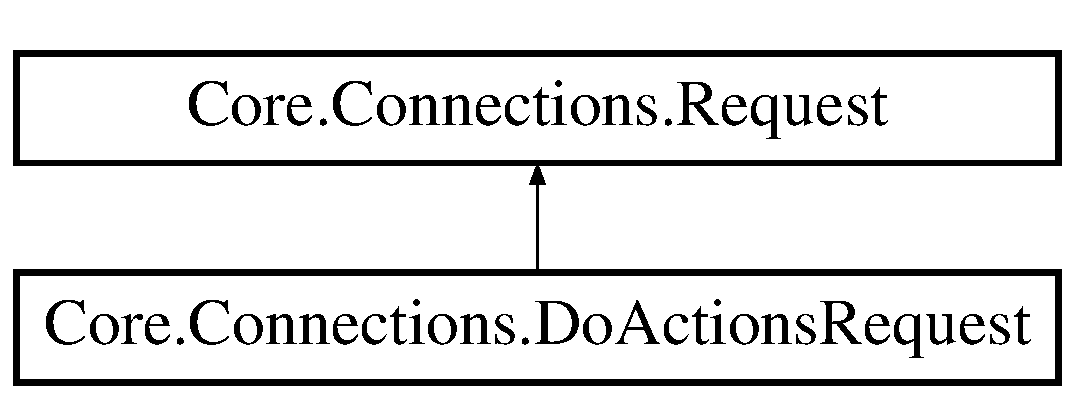
\includegraphics[height=2.000000cm]{classCore_1_1Connections_1_1DoActionsRequest}
\end{center}
\end{figure}
\subsection*{Public Member Functions}
\begin{DoxyCompactItemize}
\item 
\hyperlink{classCore_1_1Connections_1_1DoActionsRequest_a1298901ab5ab91c539caa9d5cb9115e2}{Do\+Actions\+Request} (Guid session\+I\+D, \hyperlink{classCore_1_1Models_1_1Position}{Core.\+Models.\+Position} position, \hyperlink{classCore_1_1Models_1_1Action}{Core.\+Models.\+Action}\mbox{[}$\,$\mbox{]} actions)
\begin{DoxyCompactList}\small\item\em Initializes a new instance of the \hyperlink{classCore_1_1Connections_1_1DoActionsRequest}{Core.\+Connections.\+Do\+Actions\+Request} class. \end{DoxyCompactList}\end{DoxyCompactItemize}
\subsection*{Public Attributes}
\begin{DoxyCompactItemize}
\item 
\hyperlink{classCore_1_1Models_1_1Action}{Core.\+Models.\+Action}\mbox{[}$\,$\mbox{]} \hyperlink{classCore_1_1Connections_1_1DoActionsRequest_a25fbe4ad38c5390024d7cb616507957c}{Actions}
\begin{DoxyCompactList}\small\item\em Gets or sets the actions. \end{DoxyCompactList}\end{DoxyCompactItemize}


\subsection{Detailed Description}
\hyperlink{classCore_1_1Connections_1_1Request}{Request} class which should be used to send actions to the server. Should be serialized before sending, will be deserialized after receiving. 



\subsection{Constructor \& Destructor Documentation}
\hypertarget{classCore_1_1Connections_1_1DoActionsRequest_a1298901ab5ab91c539caa9d5cb9115e2}{}\index{Core\+::\+Connections\+::\+Do\+Actions\+Request@{Core\+::\+Connections\+::\+Do\+Actions\+Request}!Do\+Actions\+Request@{Do\+Actions\+Request}}
\index{Do\+Actions\+Request@{Do\+Actions\+Request}!Core\+::\+Connections\+::\+Do\+Actions\+Request@{Core\+::\+Connections\+::\+Do\+Actions\+Request}}
\subsubsection[{Do\+Actions\+Request(\+Guid session\+I\+D, Core.\+Models.\+Position position, Core.\+Models.\+Action[] actions)}]{\setlength{\rightskip}{0pt plus 5cm}Core.\+Connections.\+Do\+Actions\+Request.\+Do\+Actions\+Request (
\begin{DoxyParamCaption}
\item[{Guid}]{session\+I\+D, }
\item[{{\bf Core.\+Models.\+Position}}]{position, }
\item[{{\bf Core.\+Models.\+Action}\mbox{[}$\,$\mbox{]}}]{actions}
\end{DoxyParamCaption}
)}\label{classCore_1_1Connections_1_1DoActionsRequest_a1298901ab5ab91c539caa9d5cb9115e2}


Initializes a new instance of the \hyperlink{classCore_1_1Connections_1_1DoActionsRequest}{Core.\+Connections.\+Do\+Actions\+Request} class. 


\begin{DoxyParams}{Parameters}
{\em session\+I\+D} & Session I\+D of the user.\\
\hline
{\em position} & Position where the user is standing (converted G\+P\+S information).\\
\hline
{\em actions} & Actions which should be executed.\\
\hline
\end{DoxyParams}


\subsection{Member Data Documentation}
\hypertarget{classCore_1_1Connections_1_1DoActionsRequest_a25fbe4ad38c5390024d7cb616507957c}{}\index{Core\+::\+Connections\+::\+Do\+Actions\+Request@{Core\+::\+Connections\+::\+Do\+Actions\+Request}!Actions@{Actions}}
\index{Actions@{Actions}!Core\+::\+Connections\+::\+Do\+Actions\+Request@{Core\+::\+Connections\+::\+Do\+Actions\+Request}}
\subsubsection[{Actions}]{\setlength{\rightskip}{0pt plus 5cm}{\bf Core.\+Models.\+Action} \mbox{[}$\,$\mbox{]} Core.\+Connections.\+Do\+Actions\+Request.\+Actions}\label{classCore_1_1Connections_1_1DoActionsRequest_a25fbe4ad38c5390024d7cb616507957c}


Gets or sets the actions. 

The actions.

The documentation for this class was generated from the following file\+:\begin{DoxyCompactItemize}
\item 
base/\+Connection/Do\+Actions\+Request.\+cs\end{DoxyCompactItemize}

\hypertarget{classclient_1_1Droid_1_1Resource_1_1Drawable}{\section{client.\-Droid.\-Resource.\-Drawable Class Reference}
\label{classclient_1_1Droid_1_1Resource_1_1Drawable}\index{client.\-Droid.\-Resource.\-Drawable@{client.\-Droid.\-Resource.\-Drawable}}
}
\subsection*{Public Attributes}
\begin{DoxyCompactItemize}
\item 
\hypertarget{classclient_1_1Droid_1_1Resource_1_1Drawable_a0af238431d23f563312001ca3a7f9e3c}{const int {\bfseries ad16} = 2130837504}\label{classclient_1_1Droid_1_1Resource_1_1Drawable_a0af238431d23f563312001ca3a7f9e3c}

\item 
\hypertarget{classclient_1_1Droid_1_1Resource_1_1Drawable_ae7440315d4b949cbd2a052d77a7e238e}{const int {\bfseries calendar\-\_\-bg\-\_\-selector} = 2130837505}\label{classclient_1_1Droid_1_1Resource_1_1Drawable_ae7440315d4b949cbd2a052d77a7e238e}

\item 
\hypertarget{classclient_1_1Droid_1_1Resource_1_1Drawable_a13031544b000add228628786d4b0da81}{const int {\bfseries Icon} = 2130837506}\label{classclient_1_1Droid_1_1Resource_1_1Drawable_a13031544b000add228628786d4b0da81}

\end{DoxyCompactItemize}


The documentation for this class was generated from the following file\-:\begin{DoxyCompactItemize}
\item 
client/client/client.\-Android/\-Resources/Resource.\-designer.\-cs\end{DoxyCompactItemize}

\hypertarget{classClient_1_1Common_1_1Models_1_1DrawNode}{}\section{Client.\+Common.\+Models.\+Draw\+Node Class Reference}
\label{classClient_1_1Common_1_1Models_1_1DrawNode}\index{Client.\+Common.\+Models.\+Draw\+Node@{Client.\+Common.\+Models.\+Draw\+Node}}


The Draw node to draw polygons.(Not in Use)  


Inheritance diagram for Client.\+Common.\+Models.\+Draw\+Node\+:\begin{figure}[H]
\begin{center}
\leavevmode
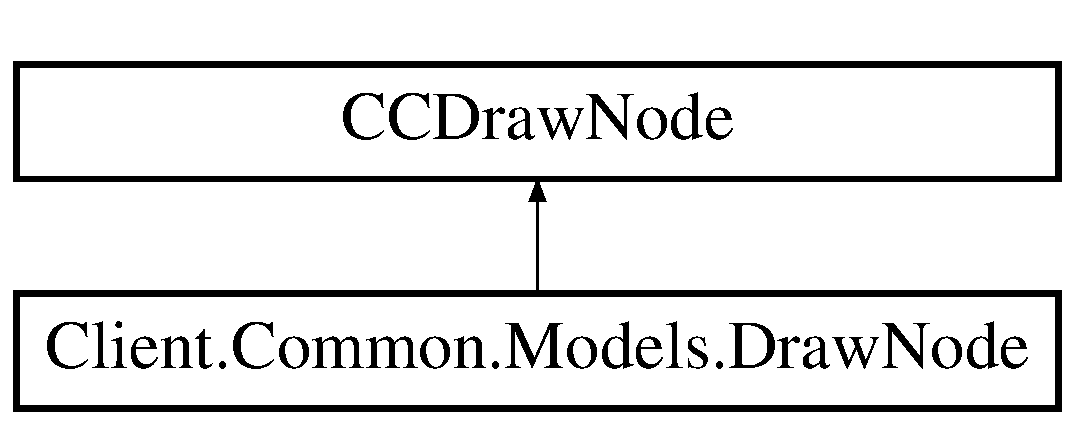
\includegraphics[height=2.000000cm]{classClient_1_1Common_1_1Models_1_1DrawNode}
\end{center}
\end{figure}
\subsection*{Public Member Functions}
\begin{DoxyCompactItemize}
\item 
\hyperlink{classClient_1_1Common_1_1Models_1_1DrawNode_a2068ce66fd508c5ecdd30c0e28604a9b}{Draw\+Node} ()
\begin{DoxyCompactList}\small\item\em Initializes a new instance of the \hyperlink{classClient_1_1Common_1_1Models_1_1DrawNode}{Client.\+Common.\+Models.\+Draw\+Node} class. \end{DoxyCompactList}\item 
void \hyperlink{classClient_1_1Common_1_1Models_1_1DrawNode_a8acad135d936298475940d5ba6b5e4d1}{Draw\+Hexagon\+For\+Hex\+Map} (C\+C\+Tile\+Map\+Layer layer, C\+C\+Tile\+Map\+Coordinates tile\+Coordinates, C\+C\+Color4\+F border\+Color, byte opacity, float border\+With)
\begin{DoxyCompactList}\small\item\em Draws the hexagon for a hex map. \end{DoxyCompactList}\item 
void \hyperlink{classClient_1_1Common_1_1Models_1_1DrawNode_af759c63ae3fc8d138925290c91bbd41f}{Draw\+Hexagon\+For\+Iso\+Stag\+Map} (float png\+Width, C\+C\+Tile\+Map\+Layer layer, C\+C\+Tile\+Map\+Coordinates tile\+Coordinates, C\+C\+Color4\+F border\+Color, byte opacity, float border\+With)
\begin{DoxyCompactList}\small\item\em Draws the hexagon for a iso stag map. \end{DoxyCompactList}\item 
void \hyperlink{classClient_1_1Common_1_1Models_1_1DrawNode_a0b4fd6fccd6e7c7f0d6a889f7bcb2ea5}{Draw\+I\+S\+O\+For\+Iso\+Stag\+Map} (float png\+Width, C\+C\+Tile\+Map\+Layer layer, C\+C\+Tile\+Map\+Coordinates tile\+Coordinates, C\+C\+Color4\+F border\+Color, byte opacity, float border\+With)
\begin{DoxyCompactList}\small\item\em Draws the I\+S\+O trapez for iso stag map. \end{DoxyCompactList}\end{DoxyCompactItemize}


\subsection{Detailed Description}
The Draw node to draw polygons.(Not in Use) 



\subsection{Constructor \& Destructor Documentation}
\hypertarget{classClient_1_1Common_1_1Models_1_1DrawNode_a2068ce66fd508c5ecdd30c0e28604a9b}{}\index{Client\+::\+Common\+::\+Models\+::\+Draw\+Node@{Client\+::\+Common\+::\+Models\+::\+Draw\+Node}!Draw\+Node@{Draw\+Node}}
\index{Draw\+Node@{Draw\+Node}!Client\+::\+Common\+::\+Models\+::\+Draw\+Node@{Client\+::\+Common\+::\+Models\+::\+Draw\+Node}}
\subsubsection[{Draw\+Node()}]{\setlength{\rightskip}{0pt plus 5cm}Client.\+Common.\+Models.\+Draw\+Node.\+Draw\+Node (
\begin{DoxyParamCaption}
{}
\end{DoxyParamCaption}
)}\label{classClient_1_1Common_1_1Models_1_1DrawNode_a2068ce66fd508c5ecdd30c0e28604a9b}


Initializes a new instance of the \hyperlink{classClient_1_1Common_1_1Models_1_1DrawNode}{Client.\+Common.\+Models.\+Draw\+Node} class. 



\subsection{Member Function Documentation}
\hypertarget{classClient_1_1Common_1_1Models_1_1DrawNode_a8acad135d936298475940d5ba6b5e4d1}{}\index{Client\+::\+Common\+::\+Models\+::\+Draw\+Node@{Client\+::\+Common\+::\+Models\+::\+Draw\+Node}!Draw\+Hexagon\+For\+Hex\+Map@{Draw\+Hexagon\+For\+Hex\+Map}}
\index{Draw\+Hexagon\+For\+Hex\+Map@{Draw\+Hexagon\+For\+Hex\+Map}!Client\+::\+Common\+::\+Models\+::\+Draw\+Node@{Client\+::\+Common\+::\+Models\+::\+Draw\+Node}}
\subsubsection[{Draw\+Hexagon\+For\+Hex\+Map(\+C\+C\+Tile\+Map\+Layer layer, C\+C\+Tile\+Map\+Coordinates tile\+Coordinates, C\+C\+Color4\+F border\+Color, byte opacity, float border\+With)}]{\setlength{\rightskip}{0pt plus 5cm}void Client.\+Common.\+Models.\+Draw\+Node.\+Draw\+Hexagon\+For\+Hex\+Map (
\begin{DoxyParamCaption}
\item[{C\+C\+Tile\+Map\+Layer}]{layer, }
\item[{C\+C\+Tile\+Map\+Coordinates}]{tile\+Coordinates, }
\item[{C\+C\+Color4\+F}]{border\+Color, }
\item[{byte}]{opacity, }
\item[{float}]{border\+With}
\end{DoxyParamCaption}
)}\label{classClient_1_1Common_1_1Models_1_1DrawNode_a8acad135d936298475940d5ba6b5e4d1}


Draws the hexagon for a hex map. 


\begin{DoxyParams}{Parameters}
{\em layer} & The layer.\\
\hline
{\em tile\+Coordinates} & The tilecoordinates.\\
\hline
{\em border\+Color} & The border color.\\
\hline
{\em opacity} & The opacity.\\
\hline
{\em border\+With} & The border with.\\
\hline
\end{DoxyParams}
\hypertarget{classClient_1_1Common_1_1Models_1_1DrawNode_af759c63ae3fc8d138925290c91bbd41f}{}\index{Client\+::\+Common\+::\+Models\+::\+Draw\+Node@{Client\+::\+Common\+::\+Models\+::\+Draw\+Node}!Draw\+Hexagon\+For\+Iso\+Stag\+Map@{Draw\+Hexagon\+For\+Iso\+Stag\+Map}}
\index{Draw\+Hexagon\+For\+Iso\+Stag\+Map@{Draw\+Hexagon\+For\+Iso\+Stag\+Map}!Client\+::\+Common\+::\+Models\+::\+Draw\+Node@{Client\+::\+Common\+::\+Models\+::\+Draw\+Node}}
\subsubsection[{Draw\+Hexagon\+For\+Iso\+Stag\+Map(float png\+Width, C\+C\+Tile\+Map\+Layer layer, C\+C\+Tile\+Map\+Coordinates tile\+Coordinates, C\+C\+Color4\+F border\+Color, byte opacity, float border\+With)}]{\setlength{\rightskip}{0pt plus 5cm}void Client.\+Common.\+Models.\+Draw\+Node.\+Draw\+Hexagon\+For\+Iso\+Stag\+Map (
\begin{DoxyParamCaption}
\item[{float}]{png\+Width, }
\item[{C\+C\+Tile\+Map\+Layer}]{layer, }
\item[{C\+C\+Tile\+Map\+Coordinates}]{tile\+Coordinates, }
\item[{C\+C\+Color4\+F}]{border\+Color, }
\item[{byte}]{opacity, }
\item[{float}]{border\+With}
\end{DoxyParamCaption}
)}\label{classClient_1_1Common_1_1Models_1_1DrawNode_af759c63ae3fc8d138925290c91bbd41f}


Draws the hexagon for a iso stag map. 


\begin{DoxyParams}{Parameters}
{\em png\+Width} & Png width.\\
\hline
{\em layer} & The layer.\\
\hline
{\em tile\+Coordinates} & Tile coordinates.\\
\hline
{\em border\+Color} & Border color.\\
\hline
{\em opacity} & The opacity.\\
\hline
{\em border\+With} & Border with.\\
\hline
\end{DoxyParams}
\hypertarget{classClient_1_1Common_1_1Models_1_1DrawNode_a0b4fd6fccd6e7c7f0d6a889f7bcb2ea5}{}\index{Client\+::\+Common\+::\+Models\+::\+Draw\+Node@{Client\+::\+Common\+::\+Models\+::\+Draw\+Node}!Draw\+I\+S\+O\+For\+Iso\+Stag\+Map@{Draw\+I\+S\+O\+For\+Iso\+Stag\+Map}}
\index{Draw\+I\+S\+O\+For\+Iso\+Stag\+Map@{Draw\+I\+S\+O\+For\+Iso\+Stag\+Map}!Client\+::\+Common\+::\+Models\+::\+Draw\+Node@{Client\+::\+Common\+::\+Models\+::\+Draw\+Node}}
\subsubsection[{Draw\+I\+S\+O\+For\+Iso\+Stag\+Map(float png\+Width, C\+C\+Tile\+Map\+Layer layer, C\+C\+Tile\+Map\+Coordinates tile\+Coordinates, C\+C\+Color4\+F border\+Color, byte opacity, float border\+With)}]{\setlength{\rightskip}{0pt plus 5cm}void Client.\+Common.\+Models.\+Draw\+Node.\+Draw\+I\+S\+O\+For\+Iso\+Stag\+Map (
\begin{DoxyParamCaption}
\item[{float}]{png\+Width, }
\item[{C\+C\+Tile\+Map\+Layer}]{layer, }
\item[{C\+C\+Tile\+Map\+Coordinates}]{tile\+Coordinates, }
\item[{C\+C\+Color4\+F}]{border\+Color, }
\item[{byte}]{opacity, }
\item[{float}]{border\+With}
\end{DoxyParamCaption}
)}\label{classClient_1_1Common_1_1Models_1_1DrawNode_a0b4fd6fccd6e7c7f0d6a889f7bcb2ea5}


Draws the I\+S\+O trapez for iso stag map. 


\begin{DoxyParams}{Parameters}
{\em png\+Width} & Png width.\\
\hline
{\em layer} & The layer.\\
\hline
{\em tile\+Coordinates} & Tile coordinates.\\
\hline
{\em border\+Color} & Border color.\\
\hline
{\em opacity} & The Opacity.\\
\hline
{\em border\+With} & Border with.\\
\hline
\end{DoxyParams}


The documentation for this class was generated from the following file\+:\begin{DoxyCompactItemize}
\item 
client/client/client.\+Common/\+Models/Draw\+Node.\+cs\end{DoxyCompactItemize}

\hypertarget{classCore_1_1Models_1_1Entity}{}\section{Core.\+Models.\+Entity Class Reference}
\label{classCore_1_1Models_1_1Entity}\index{Core.\+Models.\+Entity@{Core.\+Models.\+Entity}}


\hyperlink{classCore_1_1Models_1_1Entity}{Entity} which represents an \char`\"{}object\char`\"{} in the game world\+: units, terrain, buildings... etc.  


Inheritance diagram for Core.\+Models.\+Entity\+:\begin{figure}[H]
\begin{center}
\leavevmode
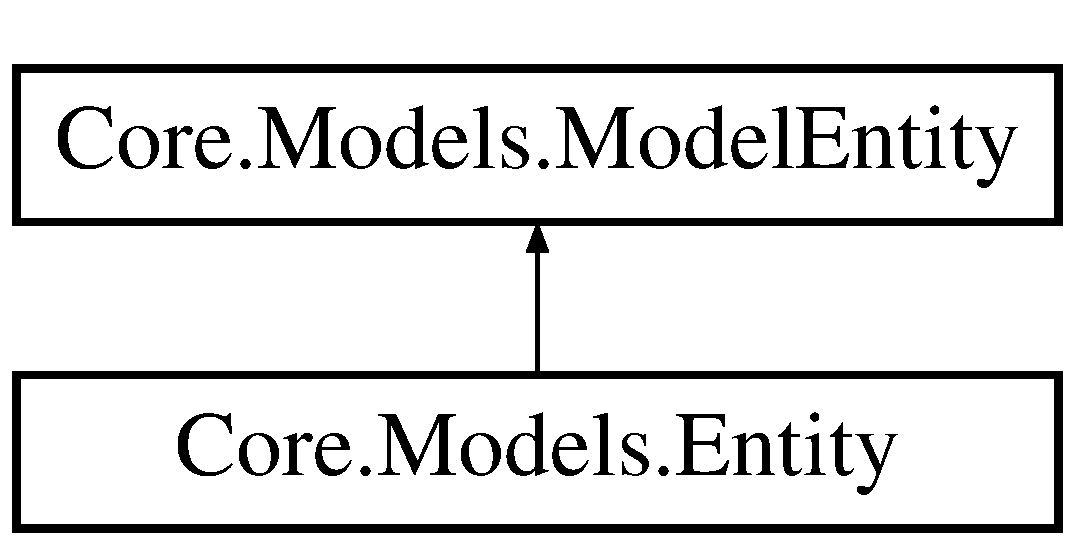
\includegraphics[height=2.000000cm]{classCore_1_1Models_1_1Entity}
\end{center}
\end{figure}
\subsection*{Public Member Functions}
\begin{DoxyCompactItemize}
\item 
\hyperlink{classCore_1_1Models_1_1Entity_ab4e03f1aca6a491f8fae7777615f1330}{Entity} (int id, \hyperlink{classCore_1_1Models_1_1Definitions_1_1Definition}{Definition} definition, \hyperlink{classCore_1_1Models_1_1Account}{Account} owner, \hyperlink{classCore_1_1Models_1_1PositionI}{Position\+I} position, int health, int move)
\begin{DoxyCompactList}\small\item\em Initializes a new instance of the \hyperlink{classCore_1_1Models_1_1Entity}{Core.\+Models.\+Entity} class. \end{DoxyCompactList}\item 
\hyperlink{classCore_1_1Models_1_1Entity_a53f50c1e8c37885db7ba432562607ccf}{Entity} (int id, int definiton\+I\+D, int owner\+I\+D, \hyperlink{classCore_1_1Models_1_1PositionI}{Position\+I} position, int health, int move)
\begin{DoxyCompactList}\small\item\em Initializes a new instance of the \hyperlink{classCore_1_1Models_1_1Entity}{Core.\+Models.\+Entity} class. \end{DoxyCompactList}\item 
\hyperlink{namespaceCore_1_1Models_ada607f76afbafc59695c90fc5a7093a2}{Diplomatic} \hyperlink{classCore_1_1Models_1_1Entity_aa05984e45fcbf9c35d6bc6cad2b323f5}{Get\+Diplomacy} (\hyperlink{classCore_1_1Models_1_1Account}{Account} account)
\begin{DoxyCompactList}\small\item\em Calculates and returns the diplomatic states between the owner of the unit and the given account \end{DoxyCompactList}\end{DoxyCompactItemize}
\subsection*{Properties}
\begin{DoxyCompactItemize}
\item 
int \hyperlink{classCore_1_1Models_1_1Entity_aa7b2cae79fc1801861c7cd20e273e3fd}{I\+D}\hspace{0.3cm}{\ttfamily  \mbox{[}get\mbox{]}}
\begin{DoxyCompactList}\small\item\em Gets the I\+D \end{DoxyCompactList}\item 
int \hyperlink{classCore_1_1Models_1_1Entity_a451f76265fc15cbcdfc1ac5233bf79e9}{Definition\+I\+D}\hspace{0.3cm}{\ttfamily  \mbox{[}get, set\mbox{]}}
\begin{DoxyCompactList}\small\item\em Gets or sets the definition I\+D. \end{DoxyCompactList}\item 
\hyperlink{classCore_1_1Models_1_1Definitions_1_1Definition}{Definition} \hyperlink{classCore_1_1Models_1_1Entity_a9d7325d3a3958dc2acfe798a2fb5a98c}{Definition}\hspace{0.3cm}{\ttfamily  \mbox{[}get\mbox{]}}
\begin{DoxyCompactList}\small\item\em Gets the definition. \end{DoxyCompactList}\item 
\hyperlink{classCore_1_1Models_1_1PositionI}{Position\+I} \hyperlink{classCore_1_1Models_1_1Entity_a0c56e42b49dbe385d0e201a42ab1feea}{Position}\hspace{0.3cm}{\ttfamily  \mbox{[}get, set\mbox{]}}
\begin{DoxyCompactList}\small\item\em Gets or sets the position. \end{DoxyCompactList}\item 
\hyperlink{classCore_1_1Models_1_1Account}{Account} \hyperlink{classCore_1_1Models_1_1Entity_af0d2b689cfd48dc43ad41c49073497df}{Owner}\hspace{0.3cm}{\ttfamily  \mbox{[}get\mbox{]}}
\begin{DoxyCompactList}\small\item\em Gets the account. \end{DoxyCompactList}\item 
int \hyperlink{classCore_1_1Models_1_1Entity_adf44e0bd8e2a08cf13fcd6a783f783e5}{Owner\+I\+D}\hspace{0.3cm}{\ttfamily  \mbox{[}get, set\mbox{]}}
\begin{DoxyCompactList}\small\item\em Gets or sets the account I. \end{DoxyCompactList}\item 
int \hyperlink{classCore_1_1Models_1_1Entity_ac054f7e992fe65ae3ffa998e4d4d1225}{Health}\hspace{0.3cm}{\ttfamily  \mbox{[}get, set\mbox{]}}
\begin{DoxyCompactList}\small\item\em Gets or sets the health. \end{DoxyCompactList}\item 
float \hyperlink{classCore_1_1Models_1_1Entity_a05336fa3c927b9f1c299f55ec27a6e0c}{Health\+Percent}\hspace{0.3cm}{\ttfamily  \mbox{[}get\mbox{]}}
\begin{DoxyCompactList}\small\item\em Gets the current health (in percent). \end{DoxyCompactList}\item 
int \hyperlink{classCore_1_1Models_1_1Entity_a3a1f85a3d32a2decd04919d03fb84167}{Move}\hspace{0.3cm}{\ttfamily  \mbox{[}get, set\mbox{]}}
\begin{DoxyCompactList}\small\item\em Gets or sets the move. \end{DoxyCompactList}\item 
int \hyperlink{classCore_1_1Models_1_1Entity_a7480e9bdfa56f0a21e784bf5cadcf3cd}{Modfied\+Attack\+Value}\hspace{0.3cm}{\ttfamily  \mbox{[}get, set\mbox{]}}
\begin{DoxyCompactList}\small\item\em Gets or sets the modified attack value. \end{DoxyCompactList}\item 
int \hyperlink{classCore_1_1Models_1_1Entity_a7bb3bab5756906f8202f48d9644fc9aa}{Modified\+Defense\+Value}\hspace{0.3cm}{\ttfamily  \mbox{[}get, set\mbox{]}}
\begin{DoxyCompactList}\small\item\em Gets or sets the modified defense value. \end{DoxyCompactList}\end{DoxyCompactItemize}
\subsection*{Additional Inherited Members}


\subsection{Detailed Description}
\hyperlink{classCore_1_1Models_1_1Entity}{Entity} which represents an \char`\"{}object\char`\"{} in the game world\+: units, terrain, buildings... etc. 



\subsection{Constructor \& Destructor Documentation}
\hypertarget{classCore_1_1Models_1_1Entity_ab4e03f1aca6a491f8fae7777615f1330}{}\index{Core\+::\+Models\+::\+Entity@{Core\+::\+Models\+::\+Entity}!Entity@{Entity}}
\index{Entity@{Entity}!Core\+::\+Models\+::\+Entity@{Core\+::\+Models\+::\+Entity}}
\subsubsection[{Entity(int id, Definition definition, Account owner, Position\+I position, int health, int move)}]{\setlength{\rightskip}{0pt plus 5cm}Core.\+Models.\+Entity.\+Entity (
\begin{DoxyParamCaption}
\item[{int}]{id, }
\item[{{\bf Definition}}]{definition, }
\item[{{\bf Account}}]{owner, }
\item[{{\bf Position\+I}}]{position, }
\item[{int}]{health, }
\item[{int}]{move}
\end{DoxyParamCaption}
)}\label{classCore_1_1Models_1_1Entity_ab4e03f1aca6a491f8fae7777615f1330}


Initializes a new instance of the \hyperlink{classCore_1_1Models_1_1Entity}{Core.\+Models.\+Entity} class. 


\begin{DoxyParams}{Parameters}
{\em id} & Identifier of the entity.\\
\hline
{\em definition} & Definition of the entity.\\
\hline
{\em owner} & Owner of the entity.\\
\hline
{\em position} & \hyperlink{classCore_1_1Models_1_1Position}{Position} of the entity.\\
\hline
{\em health} & Health of the entity.\\
\hline
{\em move} & Move of the entity.\\
\hline
\end{DoxyParams}
\hypertarget{classCore_1_1Models_1_1Entity_a53f50c1e8c37885db7ba432562607ccf}{}\index{Core\+::\+Models\+::\+Entity@{Core\+::\+Models\+::\+Entity}!Entity@{Entity}}
\index{Entity@{Entity}!Core\+::\+Models\+::\+Entity@{Core\+::\+Models\+::\+Entity}}
\subsubsection[{Entity(int id, int definiton\+I\+D, int owner\+I\+D, Position\+I position, int health, int move)}]{\setlength{\rightskip}{0pt plus 5cm}Core.\+Models.\+Entity.\+Entity (
\begin{DoxyParamCaption}
\item[{int}]{id, }
\item[{int}]{definiton\+I\+D, }
\item[{int}]{owner\+I\+D, }
\item[{{\bf Position\+I}}]{position, }
\item[{int}]{health, }
\item[{int}]{move}
\end{DoxyParamCaption}
)}\label{classCore_1_1Models_1_1Entity_a53f50c1e8c37885db7ba432562607ccf}


Initializes a new instance of the \hyperlink{classCore_1_1Models_1_1Entity}{Core.\+Models.\+Entity} class. 


\begin{DoxyParams}{Parameters}
{\em id} & Identifier of the entity.\\
\hline
{\em definiton\+I\+D} & Definiton I\+D.\\
\hline
{\em owner\+I\+D} & Owner I\+D.\\
\hline
{\em position} & \hyperlink{classCore_1_1Models_1_1Position}{Position} as integer.\\
\hline
{\em health} & Health of the entity.\\
\hline
{\em move} & Move of the entity.\\
\hline
\end{DoxyParams}


\subsection{Member Function Documentation}
\hypertarget{classCore_1_1Models_1_1Entity_aa05984e45fcbf9c35d6bc6cad2b323f5}{}\index{Core\+::\+Models\+::\+Entity@{Core\+::\+Models\+::\+Entity}!Get\+Diplomacy@{Get\+Diplomacy}}
\index{Get\+Diplomacy@{Get\+Diplomacy}!Core\+::\+Models\+::\+Entity@{Core\+::\+Models\+::\+Entity}}
\subsubsection[{Get\+Diplomacy(\+Account account)}]{\setlength{\rightskip}{0pt plus 5cm}{\bf Diplomatic} Core.\+Models.\+Entity.\+Get\+Diplomacy (
\begin{DoxyParamCaption}
\item[{{\bf Account}}]{account}
\end{DoxyParamCaption}
)}\label{classCore_1_1Models_1_1Entity_aa05984e45fcbf9c35d6bc6cad2b323f5}


Calculates and returns the diplomatic states between the owner of the unit and the given account 

\begin{DoxyReturn}{Returns}
The diplomacy.
\end{DoxyReturn}

\begin{DoxyParams}{Parameters}
{\em account} & Other \hyperlink{classCore_1_1Models_1_1Account}{Account}.\\
\hline
\end{DoxyParams}


\subsection{Property Documentation}
\hypertarget{classCore_1_1Models_1_1Entity_a9d7325d3a3958dc2acfe798a2fb5a98c}{}\index{Core\+::\+Models\+::\+Entity@{Core\+::\+Models\+::\+Entity}!Definition@{Definition}}
\index{Definition@{Definition}!Core\+::\+Models\+::\+Entity@{Core\+::\+Models\+::\+Entity}}
\subsubsection[{Definition}]{\setlength{\rightskip}{0pt plus 5cm}{\bf Definition} Core.\+Models.\+Entity.\+Definition\hspace{0.3cm}{\ttfamily [get]}}\label{classCore_1_1Models_1_1Entity_a9d7325d3a3958dc2acfe798a2fb5a98c}


Gets the definition. 

The definition.\hypertarget{classCore_1_1Models_1_1Entity_a451f76265fc15cbcdfc1ac5233bf79e9}{}\index{Core\+::\+Models\+::\+Entity@{Core\+::\+Models\+::\+Entity}!Definition\+I\+D@{Definition\+I\+D}}
\index{Definition\+I\+D@{Definition\+I\+D}!Core\+::\+Models\+::\+Entity@{Core\+::\+Models\+::\+Entity}}
\subsubsection[{Definition\+I\+D}]{\setlength{\rightskip}{0pt plus 5cm}int Core.\+Models.\+Entity.\+Definition\+I\+D\hspace{0.3cm}{\ttfamily [get]}, {\ttfamily [set]}}\label{classCore_1_1Models_1_1Entity_a451f76265fc15cbcdfc1ac5233bf79e9}


Gets or sets the definition I\+D. 

The definition I\+D.\hypertarget{classCore_1_1Models_1_1Entity_ac054f7e992fe65ae3ffa998e4d4d1225}{}\index{Core\+::\+Models\+::\+Entity@{Core\+::\+Models\+::\+Entity}!Health@{Health}}
\index{Health@{Health}!Core\+::\+Models\+::\+Entity@{Core\+::\+Models\+::\+Entity}}
\subsubsection[{Health}]{\setlength{\rightskip}{0pt plus 5cm}int Core.\+Models.\+Entity.\+Health\hspace{0.3cm}{\ttfamily [get]}, {\ttfamily [set]}}\label{classCore_1_1Models_1_1Entity_ac054f7e992fe65ae3ffa998e4d4d1225}


Gets or sets the health. 

The health.\hypertarget{classCore_1_1Models_1_1Entity_a05336fa3c927b9f1c299f55ec27a6e0c}{}\index{Core\+::\+Models\+::\+Entity@{Core\+::\+Models\+::\+Entity}!Health\+Percent@{Health\+Percent}}
\index{Health\+Percent@{Health\+Percent}!Core\+::\+Models\+::\+Entity@{Core\+::\+Models\+::\+Entity}}
\subsubsection[{Health\+Percent}]{\setlength{\rightskip}{0pt plus 5cm}float Core.\+Models.\+Entity.\+Health\+Percent\hspace{0.3cm}{\ttfamily [get]}}\label{classCore_1_1Models_1_1Entity_a05336fa3c927b9f1c299f55ec27a6e0c}


Gets the current health (in percent). 

health (in percent).\hypertarget{classCore_1_1Models_1_1Entity_aa7b2cae79fc1801861c7cd20e273e3fd}{}\index{Core\+::\+Models\+::\+Entity@{Core\+::\+Models\+::\+Entity}!I\+D@{I\+D}}
\index{I\+D@{I\+D}!Core\+::\+Models\+::\+Entity@{Core\+::\+Models\+::\+Entity}}
\subsubsection[{I\+D}]{\setlength{\rightskip}{0pt plus 5cm}int Core.\+Models.\+Entity.\+I\+D\hspace{0.3cm}{\ttfamily [get]}}\label{classCore_1_1Models_1_1Entity_aa7b2cae79fc1801861c7cd20e273e3fd}


Gets the I\+D 

The I\+D\hypertarget{classCore_1_1Models_1_1Entity_a7480e9bdfa56f0a21e784bf5cadcf3cd}{}\index{Core\+::\+Models\+::\+Entity@{Core\+::\+Models\+::\+Entity}!Modfied\+Attack\+Value@{Modfied\+Attack\+Value}}
\index{Modfied\+Attack\+Value@{Modfied\+Attack\+Value}!Core\+::\+Models\+::\+Entity@{Core\+::\+Models\+::\+Entity}}
\subsubsection[{Modfied\+Attack\+Value}]{\setlength{\rightskip}{0pt plus 5cm}int Core.\+Models.\+Entity.\+Modfied\+Attack\+Value\hspace{0.3cm}{\ttfamily [get]}, {\ttfamily [set]}}\label{classCore_1_1Models_1_1Entity_a7480e9bdfa56f0a21e784bf5cadcf3cd}


Gets or sets the modified attack value. 

The modified attack value.\hypertarget{classCore_1_1Models_1_1Entity_a7bb3bab5756906f8202f48d9644fc9aa}{}\index{Core\+::\+Models\+::\+Entity@{Core\+::\+Models\+::\+Entity}!Modified\+Defense\+Value@{Modified\+Defense\+Value}}
\index{Modified\+Defense\+Value@{Modified\+Defense\+Value}!Core\+::\+Models\+::\+Entity@{Core\+::\+Models\+::\+Entity}}
\subsubsection[{Modified\+Defense\+Value}]{\setlength{\rightskip}{0pt plus 5cm}int Core.\+Models.\+Entity.\+Modified\+Defense\+Value\hspace{0.3cm}{\ttfamily [get]}, {\ttfamily [set]}}\label{classCore_1_1Models_1_1Entity_a7bb3bab5756906f8202f48d9644fc9aa}


Gets or sets the modified defense value. 

The modified defense value.\hypertarget{classCore_1_1Models_1_1Entity_a3a1f85a3d32a2decd04919d03fb84167}{}\index{Core\+::\+Models\+::\+Entity@{Core\+::\+Models\+::\+Entity}!Move@{Move}}
\index{Move@{Move}!Core\+::\+Models\+::\+Entity@{Core\+::\+Models\+::\+Entity}}
\subsubsection[{Move}]{\setlength{\rightskip}{0pt plus 5cm}int Core.\+Models.\+Entity.\+Move\hspace{0.3cm}{\ttfamily [get]}, {\ttfamily [set]}}\label{classCore_1_1Models_1_1Entity_a3a1f85a3d32a2decd04919d03fb84167}


Gets or sets the move. 

The move.\hypertarget{classCore_1_1Models_1_1Entity_af0d2b689cfd48dc43ad41c49073497df}{}\index{Core\+::\+Models\+::\+Entity@{Core\+::\+Models\+::\+Entity}!Owner@{Owner}}
\index{Owner@{Owner}!Core\+::\+Models\+::\+Entity@{Core\+::\+Models\+::\+Entity}}
\subsubsection[{Owner}]{\setlength{\rightskip}{0pt plus 5cm}{\bf Account} Core.\+Models.\+Entity.\+Owner\hspace{0.3cm}{\ttfamily [get]}}\label{classCore_1_1Models_1_1Entity_af0d2b689cfd48dc43ad41c49073497df}


Gets the account. 

The account.\hypertarget{classCore_1_1Models_1_1Entity_adf44e0bd8e2a08cf13fcd6a783f783e5}{}\index{Core\+::\+Models\+::\+Entity@{Core\+::\+Models\+::\+Entity}!Owner\+I\+D@{Owner\+I\+D}}
\index{Owner\+I\+D@{Owner\+I\+D}!Core\+::\+Models\+::\+Entity@{Core\+::\+Models\+::\+Entity}}
\subsubsection[{Owner\+I\+D}]{\setlength{\rightskip}{0pt plus 5cm}int Core.\+Models.\+Entity.\+Owner\+I\+D\hspace{0.3cm}{\ttfamily [get]}, {\ttfamily [set]}}\label{classCore_1_1Models_1_1Entity_adf44e0bd8e2a08cf13fcd6a783f783e5}


Gets or sets the account I. 

The account I\+D.\hypertarget{classCore_1_1Models_1_1Entity_a0c56e42b49dbe385d0e201a42ab1feea}{}\index{Core\+::\+Models\+::\+Entity@{Core\+::\+Models\+::\+Entity}!Position@{Position}}
\index{Position@{Position}!Core\+::\+Models\+::\+Entity@{Core\+::\+Models\+::\+Entity}}
\subsubsection[{Position}]{\setlength{\rightskip}{0pt plus 5cm}{\bf Position\+I} Core.\+Models.\+Entity.\+Position\hspace{0.3cm}{\ttfamily [get]}, {\ttfamily [set]}}\label{classCore_1_1Models_1_1Entity_a0c56e42b49dbe385d0e201a42ab1feea}


Gets or sets the position. 

The position.

The documentation for this class was generated from the following file\+:\begin{DoxyCompactItemize}
\item 
base/\+Models/Entity.\+cs\end{DoxyCompactItemize}

\hypertarget{classClient_1_1Common_1_1Manager_1_1EntityManagerController}{}\section{Client.\+Common.\+Manager.\+Entity\+Manager\+Controller Class Reference}
\label{classClient_1_1Common_1_1Manager_1_1EntityManagerController}\index{Client.\+Common.\+Manager.\+Entity\+Manager\+Controller@{Client.\+Common.\+Manager.\+Entity\+Manager\+Controller}}


The Entity manager controller to control(load,remove,get and save) the entities.  


\subsection*{Public Member Functions}
\begin{DoxyCompactItemize}
\item 
async Task \hyperlink{classClient_1_1Common_1_1Manager_1_1EntityManagerController_a170d1ad624051207bde41fcba9882a8c}{Load\+Entities\+Async} (\hyperlink{classCore_1_1Models_1_1RegionPosition}{Region\+Position} region\+Position)
\begin{DoxyCompactList}\small\item\em Loads the entities async to the regions around the surrender center region and add the entities to these regions. \end{DoxyCompactList}\item 
async Task \hyperlink{classClient_1_1Common_1_1Manager_1_1EntityManagerController_a9082e4c083984882b905514eeb4e5ea0}{Load\+Entities\+Async} (\hyperlink{classCore_1_1Models_1_1RegionPosition}{Region\+Position}\mbox{[}$\,$\mbox{]} list\+Regions)
\begin{DoxyCompactList}\small\item\em Loads the entities async from the list of regions and add the entities to these regions. Also add the loaded actions to the view worker queue. \end{DoxyCompactList}\end{DoxyCompactItemize}
\subsection*{Properties}
\begin{DoxyCompactItemize}
\item 
static \hyperlink{classClient_1_1Common_1_1Manager_1_1EntityManagerController}{Entity\+Manager\+Controller} \hyperlink{classClient_1_1Common_1_1Manager_1_1EntityManagerController_ad3bded5714962f5182c966472f7e41d1}{Instance}\hspace{0.3cm}{\ttfamily  \mbox{[}get\mbox{]}}
\begin{DoxyCompactList}\small\item\em Gets the instance. \end{DoxyCompactList}\end{DoxyCompactItemize}


\subsection{Detailed Description}
The Entity manager controller to control(load,remove,get and save) the entities. 



\subsection{Member Function Documentation}
\hypertarget{classClient_1_1Common_1_1Manager_1_1EntityManagerController_a170d1ad624051207bde41fcba9882a8c}{}\index{Client\+::\+Common\+::\+Manager\+::\+Entity\+Manager\+Controller@{Client\+::\+Common\+::\+Manager\+::\+Entity\+Manager\+Controller}!Load\+Entities\+Async@{Load\+Entities\+Async}}
\index{Load\+Entities\+Async@{Load\+Entities\+Async}!Client\+::\+Common\+::\+Manager\+::\+Entity\+Manager\+Controller@{Client\+::\+Common\+::\+Manager\+::\+Entity\+Manager\+Controller}}
\subsubsection[{Load\+Entities\+Async(\+Region\+Position region\+Position)}]{\setlength{\rightskip}{0pt plus 5cm}async Task Client.\+Common.\+Manager.\+Entity\+Manager\+Controller.\+Load\+Entities\+Async (
\begin{DoxyParamCaption}
\item[{{\bf Region\+Position}}]{region\+Position}
\end{DoxyParamCaption}
)}\label{classClient_1_1Common_1_1Manager_1_1EntityManagerController_a170d1ad624051207bde41fcba9882a8c}


Loads the entities async to the regions around the surrender center region and add the entities to these regions. 

\begin{DoxyReturn}{Returns}
The task async.
\end{DoxyReturn}

\begin{DoxyParams}{Parameters}
{\em region\+Position} & region position.\\
\hline
\end{DoxyParams}
\hypertarget{classClient_1_1Common_1_1Manager_1_1EntityManagerController_a9082e4c083984882b905514eeb4e5ea0}{}\index{Client\+::\+Common\+::\+Manager\+::\+Entity\+Manager\+Controller@{Client\+::\+Common\+::\+Manager\+::\+Entity\+Manager\+Controller}!Load\+Entities\+Async@{Load\+Entities\+Async}}
\index{Load\+Entities\+Async@{Load\+Entities\+Async}!Client\+::\+Common\+::\+Manager\+::\+Entity\+Manager\+Controller@{Client\+::\+Common\+::\+Manager\+::\+Entity\+Manager\+Controller}}
\subsubsection[{Load\+Entities\+Async(\+Region\+Position[] list\+Regions)}]{\setlength{\rightskip}{0pt plus 5cm}async Task Client.\+Common.\+Manager.\+Entity\+Manager\+Controller.\+Load\+Entities\+Async (
\begin{DoxyParamCaption}
\item[{{\bf Region\+Position}\mbox{[}$\,$\mbox{]}}]{list\+Regions}
\end{DoxyParamCaption}
)}\label{classClient_1_1Common_1_1Manager_1_1EntityManagerController_a9082e4c083984882b905514eeb4e5ea0}


Loads the entities async from the list of regions and add the entities to these regions. Also add the loaded actions to the view worker queue. 

\begin{DoxyReturn}{Returns}
The task async.
\end{DoxyReturn}

\begin{DoxyParams}{Parameters}
{\em list\+Regions} & List of all regions which should be loaded.\\
\hline
\end{DoxyParams}


\subsection{Property Documentation}
\hypertarget{classClient_1_1Common_1_1Manager_1_1EntityManagerController_ad3bded5714962f5182c966472f7e41d1}{}\index{Client\+::\+Common\+::\+Manager\+::\+Entity\+Manager\+Controller@{Client\+::\+Common\+::\+Manager\+::\+Entity\+Manager\+Controller}!Instance@{Instance}}
\index{Instance@{Instance}!Client\+::\+Common\+::\+Manager\+::\+Entity\+Manager\+Controller@{Client\+::\+Common\+::\+Manager\+::\+Entity\+Manager\+Controller}}
\subsubsection[{Instance}]{\setlength{\rightskip}{0pt plus 5cm}{\bf Entity\+Manager\+Controller} Client.\+Common.\+Manager.\+Entity\+Manager\+Controller.\+Instance\hspace{0.3cm}{\ttfamily [static]}, {\ttfamily [get]}}\label{classClient_1_1Common_1_1Manager_1_1EntityManagerController_ad3bded5714962f5182c966472f7e41d1}


Gets the instance. 

The instance.

The documentation for this class was generated from the following file\+:\begin{DoxyCompactItemize}
\item 
client/client/client.\+Common/\+Manager/Entity\+Manager\+Controller.\+cs\end{DoxyCompactItemize}

\hypertarget{classClient_1_1Common_1_1GameAppDelegate}{\section{Client.\-Common.\-Game\-App\-Delegate Class Reference}
\label{classClient_1_1Common_1_1GameAppDelegate}\index{Client.\-Common.\-Game\-App\-Delegate@{Client.\-Common.\-Game\-App\-Delegate}}
}
Inheritance diagram for Client.\-Common.\-Game\-App\-Delegate\-:\begin{figure}[H]
\begin{center}
\leavevmode
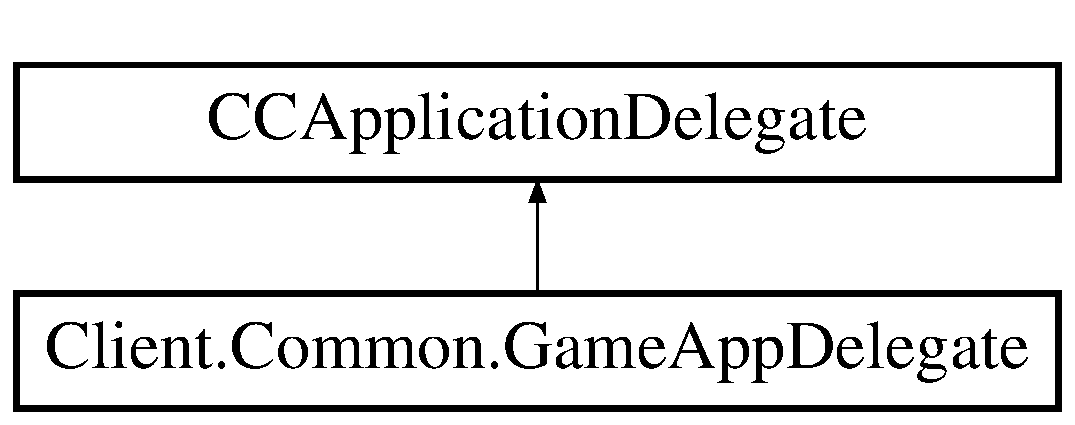
\includegraphics[height=2.000000cm]{classClient_1_1Common_1_1GameAppDelegate}
\end{center}
\end{figure}
\subsection*{Public Types}
\begin{DoxyCompactItemize}
\item 
enum {\bfseries Phases} \{ {\bfseries Start}, 
{\bfseries Start\-Scene}, 
{\bfseries Game\-Scene}, 
{\bfseries Exit}
 \}
\end{DoxyCompactItemize}
\subsection*{Public Member Functions}
\begin{DoxyCompactItemize}
\item 
\hypertarget{classClient_1_1Common_1_1GameAppDelegate_aacda9c043b12acf24de4bc13a688f52e}{override void {\bfseries Application\-Did\-Finish\-Launching} (C\-C\-Application application, C\-C\-Window main\-Window)}\label{classClient_1_1Common_1_1GameAppDelegate_aacda9c043b12acf24de4bc13a688f52e}

\item 
\hypertarget{classClient_1_1Common_1_1GameAppDelegate_a524d489c10652931d4ea5159a34a72e5}{override void {\bfseries Application\-Did\-Enter\-Background} (C\-C\-Application application)}\label{classClient_1_1Common_1_1GameAppDelegate_a524d489c10652931d4ea5159a34a72e5}

\item 
\hypertarget{classClient_1_1Common_1_1GameAppDelegate_ad2625495e6b5a1c5853acde2ace6eccb}{override void {\bfseries Application\-Will\-Enter\-Foreground} (C\-C\-Application application)}\label{classClient_1_1Common_1_1GameAppDelegate_ad2625495e6b5a1c5853acde2ace6eccb}

\end{DoxyCompactItemize}
\subsection*{Properties}
\begin{DoxyCompactItemize}
\item 
\hypertarget{classClient_1_1Common_1_1GameAppDelegate_aa626869ffdd0e3f8f46ab069bc24f0d1}{static \hyperlink{classCore_1_1Models_1_1Account}{Account} {\bfseries Account}\hspace{0.3cm}{\ttfamily  \mbox{[}get, set\mbox{]}}}\label{classClient_1_1Common_1_1GameAppDelegate_aa626869ffdd0e3f8f46ab069bc24f0d1}

\item 
\hypertarget{classClient_1_1Common_1_1GameAppDelegate_a2fb6f0fd7533c38a555760efd3ea896b}{Phases {\bfseries Phase}\hspace{0.3cm}{\ttfamily  \mbox{[}get, set\mbox{]}}}\label{classClient_1_1Common_1_1GameAppDelegate_a2fb6f0fd7533c38a555760efd3ea896b}

\end{DoxyCompactItemize}


The documentation for this class was generated from the following file\-:\begin{DoxyCompactItemize}
\item 
client/client/client.\-Common/Game\-App\-Delegate.\-cs\end{DoxyCompactItemize}

\hypertarget{classClient_1_1Common_1_1Views_1_1GameScene}{}\section{Client.\+Common.\+Views.\+Game\+Scene Class Reference}
\label{classClient_1_1Common_1_1Views_1_1GameScene}\index{Client.\+Common.\+Views.\+Game\+Scene@{Client.\+Common.\+Views.\+Game\+Scene}}


The Game scene.  


Inheritance diagram for Client.\+Common.\+Views.\+Game\+Scene\+:\begin{figure}[H]
\begin{center}
\leavevmode
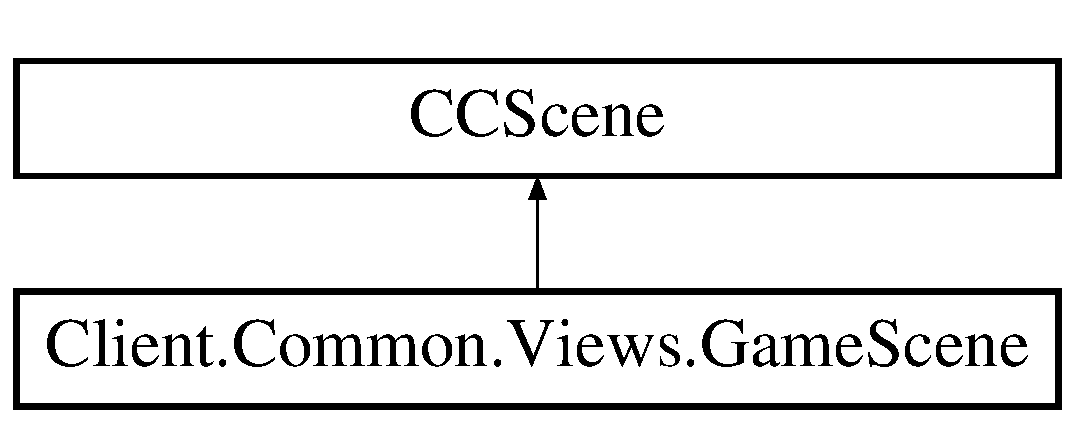
\includegraphics[height=2.000000cm]{classClient_1_1Common_1_1Views_1_1GameScene}
\end{center}
\end{figure}
\subsection*{Public Member Functions}
\begin{DoxyCompactItemize}
\item 
\hyperlink{classClient_1_1Common_1_1Views_1_1GameScene_a946494de04b027e43b5d2229cc780f7e}{Game\+Scene} (C\+C\+Window main\+Window)
\begin{DoxyCompactList}\small\item\em Initializes a new instance of the \hyperlink{classClient_1_1Common_1_1Views_1_1GameScene}{Client.\+Common.\+Views.\+Game\+Scene} class. \end{DoxyCompactList}\end{DoxyCompactItemize}
\subsection*{Public Attributes}
\begin{DoxyCompactItemize}
\item 
\hyperlink{classClient_1_1Common_1_1Views_1_1WorldLayerHex}{World\+Layer\+Hex} \hyperlink{classClient_1_1Common_1_1Views_1_1GameScene_af3de419dcf8598986518a62b075b915a}{World\+Layer\+Hex}
\begin{DoxyCompactList}\small\item\em The world in hex (whole game field). \end{DoxyCompactList}\item 
\hyperlink{classClient_1_1Common_1_1Views_1_1DebugLayer}{Debug\+Layer} \hyperlink{classClient_1_1Common_1_1Views_1_1GameScene_a69368b2f72d335939becb41659748957}{Debug\+Layer}
\begin{DoxyCompactList}\small\item\em The debug layer (shows logging information). \end{DoxyCompactList}\item 
\hyperlink{classClient_1_1Common_1_1Views_1_1HUD_1_1HUDLayer}{H\+U\+D.\+H\+U\+D\+Layer} \hyperlink{classClient_1_1Common_1_1Views_1_1GameScene_a258d6926c69733c7113ed83bd4c6940f}{H\+U\+D}
\begin{DoxyCompactList}\small\item\em The \hyperlink{namespaceClient_1_1Common_1_1Views_1_1HUD}{H\+U\+D} with all player output information. \end{DoxyCompactList}\end{DoxyCompactItemize}


\subsection{Detailed Description}
The Game scene. 



\subsection{Constructor \& Destructor Documentation}
\hypertarget{classClient_1_1Common_1_1Views_1_1GameScene_a946494de04b027e43b5d2229cc780f7e}{}\index{Client\+::\+Common\+::\+Views\+::\+Game\+Scene@{Client\+::\+Common\+::\+Views\+::\+Game\+Scene}!Game\+Scene@{Game\+Scene}}
\index{Game\+Scene@{Game\+Scene}!Client\+::\+Common\+::\+Views\+::\+Game\+Scene@{Client\+::\+Common\+::\+Views\+::\+Game\+Scene}}
\subsubsection[{Game\+Scene(\+C\+C\+Window main\+Window)}]{\setlength{\rightskip}{0pt plus 5cm}Client.\+Common.\+Views.\+Game\+Scene.\+Game\+Scene (
\begin{DoxyParamCaption}
\item[{C\+C\+Window}]{main\+Window}
\end{DoxyParamCaption}
)}\label{classClient_1_1Common_1_1Views_1_1GameScene_a946494de04b027e43b5d2229cc780f7e}


Initializes a new instance of the \hyperlink{classClient_1_1Common_1_1Views_1_1GameScene}{Client.\+Common.\+Views.\+Game\+Scene} class. 


\begin{DoxyParams}{Parameters}
{\em main\+Window} & Main window.\\
\hline
\end{DoxyParams}


\subsection{Member Data Documentation}
\hypertarget{classClient_1_1Common_1_1Views_1_1GameScene_a69368b2f72d335939becb41659748957}{}\index{Client\+::\+Common\+::\+Views\+::\+Game\+Scene@{Client\+::\+Common\+::\+Views\+::\+Game\+Scene}!Debug\+Layer@{Debug\+Layer}}
\index{Debug\+Layer@{Debug\+Layer}!Client\+::\+Common\+::\+Views\+::\+Game\+Scene@{Client\+::\+Common\+::\+Views\+::\+Game\+Scene}}
\subsubsection[{Debug\+Layer}]{\setlength{\rightskip}{0pt plus 5cm}{\bf Debug\+Layer} Client.\+Common.\+Views.\+Game\+Scene.\+Debug\+Layer}\label{classClient_1_1Common_1_1Views_1_1GameScene_a69368b2f72d335939becb41659748957}


The debug layer (shows logging information). 

\hypertarget{classClient_1_1Common_1_1Views_1_1GameScene_a258d6926c69733c7113ed83bd4c6940f}{}\index{Client\+::\+Common\+::\+Views\+::\+Game\+Scene@{Client\+::\+Common\+::\+Views\+::\+Game\+Scene}!H\+U\+D@{H\+U\+D}}
\index{H\+U\+D@{H\+U\+D}!Client\+::\+Common\+::\+Views\+::\+Game\+Scene@{Client\+::\+Common\+::\+Views\+::\+Game\+Scene}}
\subsubsection[{H\+U\+D}]{\setlength{\rightskip}{0pt plus 5cm}{\bf H\+U\+D.\+H\+U\+D\+Layer} Client.\+Common.\+Views.\+Game\+Scene.\+H\+U\+D}\label{classClient_1_1Common_1_1Views_1_1GameScene_a258d6926c69733c7113ed83bd4c6940f}


The \hyperlink{namespaceClient_1_1Common_1_1Views_1_1HUD}{H\+U\+D} with all player output information. 

\hypertarget{classClient_1_1Common_1_1Views_1_1GameScene_af3de419dcf8598986518a62b075b915a}{}\index{Client\+::\+Common\+::\+Views\+::\+Game\+Scene@{Client\+::\+Common\+::\+Views\+::\+Game\+Scene}!World\+Layer\+Hex@{World\+Layer\+Hex}}
\index{World\+Layer\+Hex@{World\+Layer\+Hex}!Client\+::\+Common\+::\+Views\+::\+Game\+Scene@{Client\+::\+Common\+::\+Views\+::\+Game\+Scene}}
\subsubsection[{World\+Layer\+Hex}]{\setlength{\rightskip}{0pt plus 5cm}{\bf World\+Layer\+Hex} Client.\+Common.\+Views.\+Game\+Scene.\+World\+Layer\+Hex}\label{classClient_1_1Common_1_1Views_1_1GameScene_af3de419dcf8598986518a62b075b915a}


The world in hex (whole game field). 



The documentation for this class was generated from the following file\+:\begin{DoxyCompactItemize}
\item 
client/client/client.\+Common/\+Views/Game\+Scene.\+cs\end{DoxyCompactItemize}

\hypertarget{classClient_1_1Common_1_1Models_1_1Geolocation}{\section{Client.\-Common.\-Models.\-Geolocation Class Reference}
\label{classClient_1_1Common_1_1Models_1_1Geolocation}\index{Client.\-Common.\-Models.\-Geolocation@{Client.\-Common.\-Models.\-Geolocation}}
}
Inheritance diagram for Client.\-Common.\-Models.\-Geolocation\-:\begin{figure}[H]
\begin{center}
\leavevmode
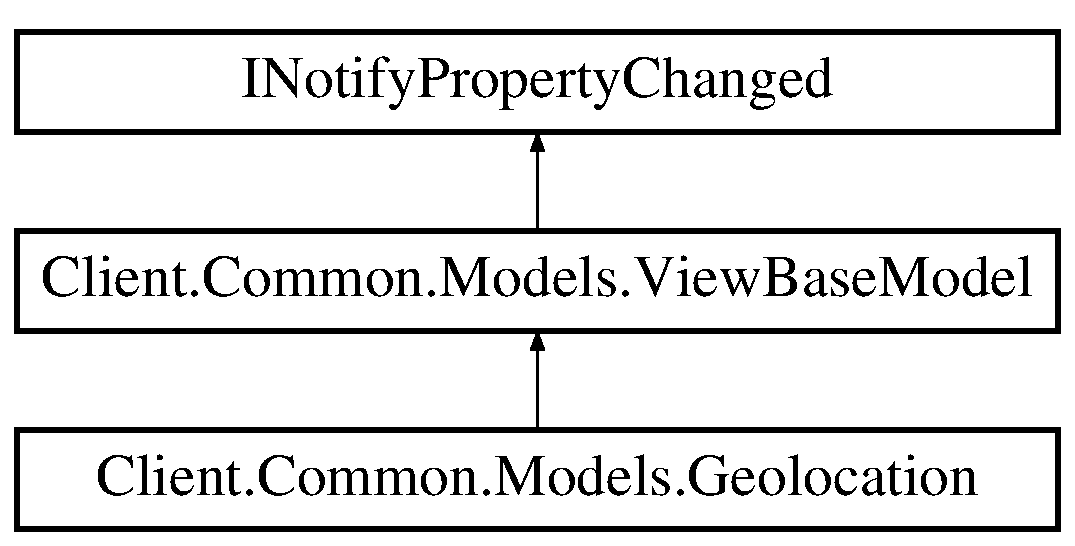
\includegraphics[height=3.000000cm]{classClient_1_1Common_1_1Models_1_1Geolocation}
\end{center}
\end{figure}
\subsection*{Public Member Functions}
\begin{DoxyCompactItemize}
\item 
\hypertarget{classClient_1_1Common_1_1Models_1_1Geolocation_aed14d4e1cc101de935133d0fae3ef349}{void {\bfseries Start\-Listening} (uint min\-Time\-Intervall\-In\-Milli\-Sec, double min\-Distance)}\label{classClient_1_1Common_1_1Models_1_1Geolocation_aed14d4e1cc101de935133d0fae3ef349}

\item 
\hypertarget{classClient_1_1Common_1_1Models_1_1Geolocation_a6b6da0803d978de553791129b51954e9}{void {\bfseries Stop\-Listening} ()}\label{classClient_1_1Common_1_1Models_1_1Geolocation_a6b6da0803d978de553791129b51954e9}

\end{DoxyCompactItemize}
\subsection*{Static Public Attributes}
\begin{DoxyCompactItemize}
\item 
\hypertarget{classClient_1_1Common_1_1Models_1_1Geolocation_a3f4999c40384dacf2bfbcc8541ec9d36}{static string {\bfseries Property\-Name\-Current\-Position} = \char`\"{}Current\-Position\char`\"{}}\label{classClient_1_1Common_1_1Models_1_1Geolocation_a3f4999c40384dacf2bfbcc8541ec9d36}

\item 
\hypertarget{classClient_1_1Common_1_1Models_1_1Geolocation_a7b6f72dc9388e33dc973df7b181ce411}{static string {\bfseries Property\-Name\-Current\-Game\-Position} = \char`\"{}Current\-Game\-Position\char`\"{}}\label{classClient_1_1Common_1_1Models_1_1Geolocation_a7b6f72dc9388e33dc973df7b181ce411}

\item 
\hypertarget{classClient_1_1Common_1_1Models_1_1Geolocation_a5353dece1f4b5136523b203c286fd286}{static string {\bfseries Property\-Name\-Current\-Region\-Position} = \char`\"{}Current\-Region\-Position\char`\"{}}\label{classClient_1_1Common_1_1Models_1_1Geolocation_a5353dece1f4b5136523b203c286fd286}

\item 
\hypertarget{classClient_1_1Common_1_1Models_1_1Geolocation_ada75530b4ed8ed2325645a2e36347638}{static string {\bfseries Property\-Name\-Current\-Cell\-Position} = \char`\"{}Current\-Cell\-Position\char`\"{}}\label{classClient_1_1Common_1_1Models_1_1Geolocation_ada75530b4ed8ed2325645a2e36347638}

\item 
\hypertarget{classClient_1_1Common_1_1Models_1_1Geolocation_a798075f80d9cd9bdb31ed9b63702640e}{static string {\bfseries Property\-Name\-Last\-Position} = \char`\"{}Last\-Position\char`\"{}}\label{classClient_1_1Common_1_1Models_1_1Geolocation_a798075f80d9cd9bdb31ed9b63702640e}

\item 
\hypertarget{classClient_1_1Common_1_1Models_1_1Geolocation_abe0697da656646d1f68449e24b85f7ff}{static string {\bfseries Property\-Name\-Last\-Game\-Position} = \char`\"{}Last\-Game\-Position\char`\"{}}\label{classClient_1_1Common_1_1Models_1_1Geolocation_abe0697da656646d1f68449e24b85f7ff}

\item 
\hypertarget{classClient_1_1Common_1_1Models_1_1Geolocation_ab9677c60c06fcf4dfe858b173b77eabe}{static string {\bfseries Property\-Name\-Last\-Region\-Position} = \char`\"{}Last\-Region\-Position\char`\"{}}\label{classClient_1_1Common_1_1Models_1_1Geolocation_ab9677c60c06fcf4dfe858b173b77eabe}

\item 
\hypertarget{classClient_1_1Common_1_1Models_1_1Geolocation_a38d84853f94027baa3c60adc8f02d6e3}{static string {\bfseries Property\-Name\-Last\-Cell\-Position} = \char`\"{}Last\-Cell\-Position\char`\"{}}\label{classClient_1_1Common_1_1Models_1_1Geolocation_a38d84853f94027baa3c60adc8f02d6e3}

\item 
\hypertarget{classClient_1_1Common_1_1Models_1_1Geolocation_a8a401890e424cd054d2e325e1dc01f8e}{static string {\bfseries Property\-Name\-Latitude} = \char`\"{}Latitude\char`\"{}}\label{classClient_1_1Common_1_1Models_1_1Geolocation_a8a401890e424cd054d2e325e1dc01f8e}

\item 
\hypertarget{classClient_1_1Common_1_1Models_1_1Geolocation_a594d0a04417db0077fe86441242360d3}{static string {\bfseries Property\-Name\-Longitude} = \char`\"{}Longitude\char`\"{}}\label{classClient_1_1Common_1_1Models_1_1Geolocation_a594d0a04417db0077fe86441242360d3}

\item 
\hypertarget{classClient_1_1Common_1_1Models_1_1Geolocation_a4bf4647ed209c7eb632edddda3d8b729}{static string {\bfseries Property\-Name\-String\-Game\-Position} = \char`\"{}String\-Game\-Position\char`\"{}}\label{classClient_1_1Common_1_1Models_1_1Geolocation_a4bf4647ed209c7eb632edddda3d8b729}

\item 
\hypertarget{classClient_1_1Common_1_1Models_1_1Geolocation_a3316a606ae6b12d6f04329fd1e4ace9a}{static string {\bfseries Property\-Name\-Altitude} = \char`\"{}Altitude\char`\"{}}\label{classClient_1_1Common_1_1Models_1_1Geolocation_a3316a606ae6b12d6f04329fd1e4ace9a}

\item 
\hypertarget{classClient_1_1Common_1_1Models_1_1Geolocation_a6833e8a264e1e993617e1711c00e1879}{static string {\bfseries Property\-Name\-Time\-Stamp} = \char`\"{}Time\-Stamp\char`\"{}}\label{classClient_1_1Common_1_1Models_1_1Geolocation_a6833e8a264e1e993617e1711c00e1879}

\item 
\hypertarget{classClient_1_1Common_1_1Models_1_1Geolocation_a55d811ef3d1bd3c993ec063acc79e144}{static string {\bfseries Property\-Name\-Heading} = \char`\"{}Heading\char`\"{}}\label{classClient_1_1Common_1_1Models_1_1Geolocation_a55d811ef3d1bd3c993ec063acc79e144}

\item 
\hypertarget{classClient_1_1Common_1_1Models_1_1Geolocation_adc17f7517c4212746606e8545037d657}{static string {\bfseries Property\-Name\-Accuracy} = \char`\"{}Accuracy\char`\"{}}\label{classClient_1_1Common_1_1Models_1_1Geolocation_adc17f7517c4212746606e8545037d657}

\item 
\hypertarget{classClient_1_1Common_1_1Models_1_1Geolocation_aefd68c35a83db96e6a53d95f081f906f}{static string {\bfseries Property\-Name\-Status} = \char`\"{}Status\char`\"{}}\label{classClient_1_1Common_1_1Models_1_1Geolocation_aefd68c35a83db96e6a53d95f081f906f}

\end{DoxyCompactItemize}
\subsection*{Properties}
\begin{DoxyCompactItemize}
\item 
\hypertarget{classClient_1_1Common_1_1Models_1_1Geolocation_a9ecc93738f9ed1abc9c247ffa416ec61}{static \hyperlink{classClient_1_1Common_1_1Models_1_1Geolocation}{Geolocation} {\bfseries Instance}\hspace{0.3cm}{\ttfamily  \mbox{[}get\mbox{]}}}\label{classClient_1_1Common_1_1Models_1_1Geolocation_a9ecc93738f9ed1abc9c247ffa416ec61}

\item 
\hypertarget{classClient_1_1Common_1_1Models_1_1Geolocation_af23e9f046c7ba9175e28f4d8be2b50c6}{bool {\bfseries Is\-Busy}\hspace{0.3cm}{\ttfamily  \mbox{[}get, set\mbox{]}}}\label{classClient_1_1Common_1_1Models_1_1Geolocation_af23e9f046c7ba9175e28f4d8be2b50c6}

\item 
\hypertarget{classClient_1_1Common_1_1Models_1_1Geolocation_a85bd8180428cd914f2853273dc77a152}{bool {\bfseries Is\-Position\-Changed}\hspace{0.3cm}{\ttfamily  \mbox{[}get, set\mbox{]}}}\label{classClient_1_1Common_1_1Models_1_1Geolocation_a85bd8180428cd914f2853273dc77a152}

\item 
\hypertarget{classClient_1_1Common_1_1Models_1_1Geolocation_ac61d7c4a25a8a8a3db55177ec8f0fb40}{bool {\bfseries Is\-Geolocation\-Available}\hspace{0.3cm}{\ttfamily  \mbox{[}get\mbox{]}}}\label{classClient_1_1Common_1_1Models_1_1Geolocation_ac61d7c4a25a8a8a3db55177ec8f0fb40}

\item 
\hypertarget{classClient_1_1Common_1_1Models_1_1Geolocation_a4d17b1f0ad9cb37ed4d67097266ef214}{bool {\bfseries Is\-Geolocation\-Enabled}\hspace{0.3cm}{\ttfamily  \mbox{[}get\mbox{]}}}\label{classClient_1_1Common_1_1Models_1_1Geolocation_a4d17b1f0ad9cb37ed4d67097266ef214}

\item 
\hypertarget{classClient_1_1Common_1_1Models_1_1Geolocation_a1d0e7e5bfd5ae8c366169c4c4a1d1747}{bool {\bfseries Is\-Geolocation\-Listening}\hspace{0.3cm}{\ttfamily  \mbox{[}get\mbox{]}}}\label{classClient_1_1Common_1_1Models_1_1Geolocation_a1d0e7e5bfd5ae8c366169c4c4a1d1747}

\item 
\hypertarget{classClient_1_1Common_1_1Models_1_1Geolocation_ad1d6a64ce5a9764cc8bae0a0ea4a70a2}{int {\bfseries Id}\hspace{0.3cm}{\ttfamily  \mbox{[}get, set\mbox{]}}}\label{classClient_1_1Common_1_1Models_1_1Geolocation_ad1d6a64ce5a9764cc8bae0a0ea4a70a2}

\item 
\hypertarget{classClient_1_1Common_1_1Models_1_1Geolocation_a481303a3e49d4ab404050ca8ca7d3e86}{Position {\bfseries Current\-Position}\hspace{0.3cm}{\ttfamily  \mbox{[}get, set\mbox{]}}}\label{classClient_1_1Common_1_1Models_1_1Geolocation_a481303a3e49d4ab404050ca8ca7d3e86}

\item 
\hypertarget{classClient_1_1Common_1_1Models_1_1Geolocation_ad14334db3507a02eb7ecf245d0e4154c}{\hyperlink{classCore_1_1Models_1_1Position}{Core.\-Models.\-Position} {\bfseries Current\-Game\-Position}\hspace{0.3cm}{\ttfamily  \mbox{[}get, set\mbox{]}}}\label{classClient_1_1Common_1_1Models_1_1Geolocation_ad14334db3507a02eb7ecf245d0e4154c}

\item 
\hypertarget{classClient_1_1Common_1_1Models_1_1Geolocation_accfb783b87b9df12f895053cb865f016}{\hyperlink{classCore_1_1Models_1_1RegionPosition}{Core.\-Models.\-Region\-Position} {\bfseries Current\-Region\-Position}\hspace{0.3cm}{\ttfamily  \mbox{[}get, set\mbox{]}}}\label{classClient_1_1Common_1_1Models_1_1Geolocation_accfb783b87b9df12f895053cb865f016}

\item 
\hypertarget{classClient_1_1Common_1_1Models_1_1Geolocation_af3cd420ed76212d5399fbceea41ba03a}{\hyperlink{classCore_1_1Models_1_1CellPosition}{Core.\-Models.\-Cell\-Position} {\bfseries Current\-Cell\-Position}\hspace{0.3cm}{\ttfamily  \mbox{[}get, set\mbox{]}}}\label{classClient_1_1Common_1_1Models_1_1Geolocation_af3cd420ed76212d5399fbceea41ba03a}

\item 
\hypertarget{classClient_1_1Common_1_1Models_1_1Geolocation_ac05323e0dbb238fae5123a514aac3eaf}{Position {\bfseries Last\-Position}\hspace{0.3cm}{\ttfamily  \mbox{[}get, set\mbox{]}}}\label{classClient_1_1Common_1_1Models_1_1Geolocation_ac05323e0dbb238fae5123a514aac3eaf}

\item 
\hypertarget{classClient_1_1Common_1_1Models_1_1Geolocation_a577d828c7e1b51a10bd7444a10278548}{\hyperlink{classCore_1_1Models_1_1Position}{Core.\-Models.\-Position} {\bfseries Last\-Game\-Position}\hspace{0.3cm}{\ttfamily  \mbox{[}get, set\mbox{]}}}\label{classClient_1_1Common_1_1Models_1_1Geolocation_a577d828c7e1b51a10bd7444a10278548}

\item 
\hypertarget{classClient_1_1Common_1_1Models_1_1Geolocation_a37781ed0d4705776dabe76b1291ad5da}{\hyperlink{classCore_1_1Models_1_1RegionPosition}{Core.\-Models.\-Region\-Position} {\bfseries Last\-Region\-Position}\hspace{0.3cm}{\ttfamily  \mbox{[}get, set\mbox{]}}}\label{classClient_1_1Common_1_1Models_1_1Geolocation_a37781ed0d4705776dabe76b1291ad5da}

\item 
\hypertarget{classClient_1_1Common_1_1Models_1_1Geolocation_aa14cd6c1f33d576b14b12528654bda50}{\hyperlink{classCore_1_1Models_1_1CellPosition}{Core.\-Models.\-Cell\-Position} {\bfseries Last\-Cell\-Position}\hspace{0.3cm}{\ttfamily  \mbox{[}get, set\mbox{]}}}\label{classClient_1_1Common_1_1Models_1_1Geolocation_aa14cd6c1f33d576b14b12528654bda50}

\item 
\hypertarget{classClient_1_1Common_1_1Models_1_1Geolocation_a838a5734aea2d628c1f1f74666ee872d}{string {\bfseries Latitude}\hspace{0.3cm}{\ttfamily  \mbox{[}get, set\mbox{]}}}\label{classClient_1_1Common_1_1Models_1_1Geolocation_a838a5734aea2d628c1f1f74666ee872d}

\item 
\hypertarget{classClient_1_1Common_1_1Models_1_1Geolocation_ad21ed8fd7165bc867d3013698878a9b8}{string {\bfseries Longitude}\hspace{0.3cm}{\ttfamily  \mbox{[}get, set\mbox{]}}}\label{classClient_1_1Common_1_1Models_1_1Geolocation_ad21ed8fd7165bc867d3013698878a9b8}

\item 
\hypertarget{classClient_1_1Common_1_1Models_1_1Geolocation_ad98017ae0b14094179d1e4ff48609fa6}{string {\bfseries Altitude}\hspace{0.3cm}{\ttfamily  \mbox{[}get, set\mbox{]}}}\label{classClient_1_1Common_1_1Models_1_1Geolocation_ad98017ae0b14094179d1e4ff48609fa6}

\item 
\hypertarget{classClient_1_1Common_1_1Models_1_1Geolocation_a94c3ecddd6408b5df3c3e3b3a135f5be}{string {\bfseries String\-Game\-Position}\hspace{0.3cm}{\ttfamily  \mbox{[}get, set\mbox{]}}}\label{classClient_1_1Common_1_1Models_1_1Geolocation_a94c3ecddd6408b5df3c3e3b3a135f5be}

\item 
\hypertarget{classClient_1_1Common_1_1Models_1_1Geolocation_a3b20a3c7eb700502c6362c44f25df4f5}{string {\bfseries Time\-Stamp}\hspace{0.3cm}{\ttfamily  \mbox{[}get, set\mbox{]}}}\label{classClient_1_1Common_1_1Models_1_1Geolocation_a3b20a3c7eb700502c6362c44f25df4f5}

\item 
\hypertarget{classClient_1_1Common_1_1Models_1_1Geolocation_a61cd544e271fff1bd80e2dd30159c360}{string {\bfseries Heading}\hspace{0.3cm}{\ttfamily  \mbox{[}get, set\mbox{]}}}\label{classClient_1_1Common_1_1Models_1_1Geolocation_a61cd544e271fff1bd80e2dd30159c360}

\item 
\hypertarget{classClient_1_1Common_1_1Models_1_1Geolocation_aac245b5fd2c8fbc0c67ff14f46aec4b9}{string {\bfseries Accuracy}\hspace{0.3cm}{\ttfamily  \mbox{[}get, set\mbox{]}}}\label{classClient_1_1Common_1_1Models_1_1Geolocation_aac245b5fd2c8fbc0c67ff14f46aec4b9}

\item 
\hypertarget{classClient_1_1Common_1_1Models_1_1Geolocation_ab0d1261cf734929820b22f0d0e8dee59}{string {\bfseries Status}\hspace{0.3cm}{\ttfamily  \mbox{[}get, set\mbox{]}}}\label{classClient_1_1Common_1_1Models_1_1Geolocation_ab0d1261cf734929820b22f0d0e8dee59}

\end{DoxyCompactItemize}
\subsection*{Additional Inherited Members}


The documentation for this class was generated from the following file\-:\begin{DoxyCompactItemize}
\item 
client/client/client.\-Common/\-Models/Geolocation.\-cs\end{DoxyCompactItemize}

\hypertarget{classServer_1_1Controllers_1_1HomeController}{\section{Server.\-Controllers.\-Home\-Controller Class Reference}
\label{classServer_1_1Controllers_1_1HomeController}\index{Server.\-Controllers.\-Home\-Controller@{Server.\-Controllers.\-Home\-Controller}}
}
Inheritance diagram for Server.\-Controllers.\-Home\-Controller\-:\begin{figure}[H]
\begin{center}
\leavevmode
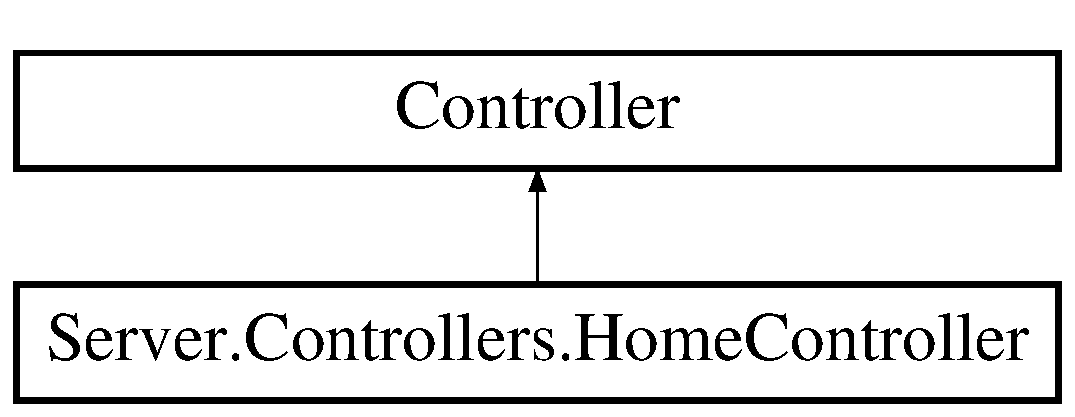
\includegraphics[height=2.000000cm]{classServer_1_1Controllers_1_1HomeController}
\end{center}
\end{figure}
\subsection*{Public Member Functions}
\begin{DoxyCompactItemize}
\item 
\hypertarget{classServer_1_1Controllers_1_1HomeController_a8c65a76479bf96d7e30952823d1009a2}{Action\-Result {\bfseries Index} ()}\label{classServer_1_1Controllers_1_1HomeController_a8c65a76479bf96d7e30952823d1009a2}

\end{DoxyCompactItemize}


The documentation for this class was generated from the following file\-:\begin{DoxyCompactItemize}
\item 
server/\-Controllers/Home\-Controller.\-cs\end{DoxyCompactItemize}

\hypertarget{classServer_1_1Controllers_1_1HTTPController}{\section{Server.\-Controllers.\-H\-T\-T\-P\-Controller Class Reference}
\label{classServer_1_1Controllers_1_1HTTPController}\index{Server.\-Controllers.\-H\-T\-T\-P\-Controller@{Server.\-Controllers.\-H\-T\-T\-P\-Controller}}
}


Handles all H\-T\-T\-P Accesses from the client.  


Inheritance diagram for Server.\-Controllers.\-H\-T\-T\-P\-Controller\-:\begin{figure}[H]
\begin{center}
\leavevmode
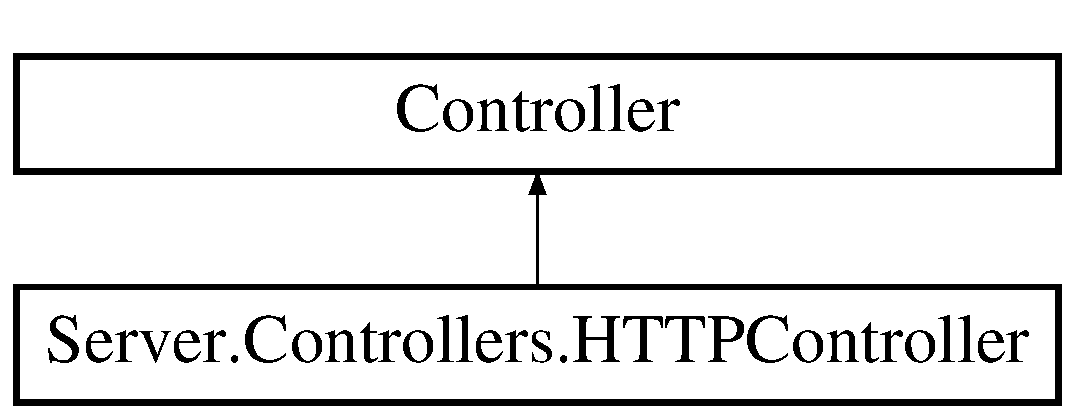
\includegraphics[height=2.000000cm]{classServer_1_1Controllers_1_1HTTPController}
\end{center}
\end{figure}
\subsection*{Public Member Functions}
\begin{DoxyCompactItemize}
\item 
\hypertarget{classServer_1_1Controllers_1_1HTTPController_a6453154b955fdc0489918911ada9a2fe}{string {\bfseries Login} ()}\label{classServer_1_1Controllers_1_1HTTPController_a6453154b955fdc0489918911ada9a2fe}

\item 
\hypertarget{classServer_1_1Controllers_1_1HTTPController_a78d73441582128cbd993f76945bf02b2}{string {\bfseries Load\-Regions} ()}\label{classServer_1_1Controllers_1_1HTTPController_a78d73441582128cbd993f76945bf02b2}

\item 
\hypertarget{classServer_1_1Controllers_1_1HTTPController_abe809c376d42128665af872585ebe0a4}{string {\bfseries Do\-Actions} ()}\label{classServer_1_1Controllers_1_1HTTPController_abe809c376d42128665af872585ebe0a4}

\item 
\hypertarget{classServer_1_1Controllers_1_1HTTPController_a040798f6ea7252caeaebee82d637957f}{string {\bfseries Error} (string json)}\label{classServer_1_1Controllers_1_1HTTPController_a040798f6ea7252caeaebee82d637957f}

\end{DoxyCompactItemize}


\subsection{Detailed Description}
Handles all H\-T\-T\-P Accesses from the client. 



The documentation for this class was generated from the following file\-:\begin{DoxyCompactItemize}
\item 
server/\-Controllers/H\-T\-T\-P\-Controller.\-cs\end{DoxyCompactItemize}

\hypertarget{classClient_1_1Droid_1_1Resource_1_1Id}{}\section{Client.\+Droid.\+Resource.\+Id Class Reference}
\label{classClient_1_1Droid_1_1Resource_1_1Id}\index{Client.\+Droid.\+Resource.\+Id@{Client.\+Droid.\+Resource.\+Id}}
\subsection*{Public Attributes}
\begin{DoxyCompactItemize}
\item 
\hypertarget{classClient_1_1Droid_1_1Resource_1_1Id_aae8bbd33832b4a37185d54124bdd9b17}{}const int {\bfseries action0} = 2131296376\label{classClient_1_1Droid_1_1Resource_1_1Id_aae8bbd33832b4a37185d54124bdd9b17}

\item 
\hypertarget{classClient_1_1Droid_1_1Resource_1_1Id_addcceb1ced6a8206d89bda289ad23957}{}const int {\bfseries action\+\_\+bar} = 2131296341\label{classClient_1_1Droid_1_1Resource_1_1Id_addcceb1ced6a8206d89bda289ad23957}

\item 
\hypertarget{classClient_1_1Droid_1_1Resource_1_1Id_a21c161b728248082bbfdecd13fec9caf}{}const int {\bfseries action\+\_\+bar\+\_\+activity\+\_\+content} = 2131296257\label{classClient_1_1Droid_1_1Resource_1_1Id_a21c161b728248082bbfdecd13fec9caf}

\item 
\hypertarget{classClient_1_1Droid_1_1Resource_1_1Id_a3d0d413002563020efea50dc0fb3e3b6}{}const int {\bfseries action\+\_\+bar\+\_\+container} = 2131296340\label{classClient_1_1Droid_1_1Resource_1_1Id_a3d0d413002563020efea50dc0fb3e3b6}

\item 
\hypertarget{classClient_1_1Droid_1_1Resource_1_1Id_a1342a114a204d41f363dcae2d4ee8f32}{}const int {\bfseries action\+\_\+bar\+\_\+root} = 2131296336\label{classClient_1_1Droid_1_1Resource_1_1Id_a1342a114a204d41f363dcae2d4ee8f32}

\item 
\hypertarget{classClient_1_1Droid_1_1Resource_1_1Id_a9a469afced0ae50ae598761a8c337c8e}{}const int {\bfseries action\+\_\+bar\+\_\+spinner} = 2131296258\label{classClient_1_1Droid_1_1Resource_1_1Id_a9a469afced0ae50ae598761a8c337c8e}

\item 
\hypertarget{classClient_1_1Droid_1_1Resource_1_1Id_a160a5ed93e83159f6f6c1ad728fa6109}{}const int {\bfseries action\+\_\+bar\+\_\+subtitle} = 2131296313\label{classClient_1_1Droid_1_1Resource_1_1Id_a160a5ed93e83159f6f6c1ad728fa6109}

\item 
\hypertarget{classClient_1_1Droid_1_1Resource_1_1Id_a3df19fa63d2c951bed72dd4a322bad97}{}const int {\bfseries action\+\_\+bar\+\_\+title} = 2131296312\label{classClient_1_1Droid_1_1Resource_1_1Id_a3df19fa63d2c951bed72dd4a322bad97}

\item 
\hypertarget{classClient_1_1Droid_1_1Resource_1_1Id_ad6239c17b1cd64fd86bb6b48faba3eff}{}const int {\bfseries action\+\_\+context\+\_\+bar} = 2131296342\label{classClient_1_1Droid_1_1Resource_1_1Id_ad6239c17b1cd64fd86bb6b48faba3eff}

\item 
\hypertarget{classClient_1_1Droid_1_1Resource_1_1Id_a01ceb520fbdb25673976967fbd668d23}{}const int {\bfseries action\+\_\+divider} = 2131296380\label{classClient_1_1Droid_1_1Resource_1_1Id_a01ceb520fbdb25673976967fbd668d23}

\item 
\hypertarget{classClient_1_1Droid_1_1Resource_1_1Id_ad8af00473227d79958b069df09feeb2a}{}const int {\bfseries action\+\_\+menu\+\_\+divider} = 2131296259\label{classClient_1_1Droid_1_1Resource_1_1Id_ad8af00473227d79958b069df09feeb2a}

\item 
\hypertarget{classClient_1_1Droid_1_1Resource_1_1Id_a386e89594c3c4583a7aa21b73fdaa3a7}{}const int {\bfseries action\+\_\+menu\+\_\+presenter} = 2131296260\label{classClient_1_1Droid_1_1Resource_1_1Id_a386e89594c3c4583a7aa21b73fdaa3a7}

\item 
\hypertarget{classClient_1_1Droid_1_1Resource_1_1Id_ad67742fd0acd3f5363f61fd593d1ea50}{}const int {\bfseries action\+\_\+mode\+\_\+bar} = 2131296338\label{classClient_1_1Droid_1_1Resource_1_1Id_ad67742fd0acd3f5363f61fd593d1ea50}

\item 
\hypertarget{classClient_1_1Droid_1_1Resource_1_1Id_a096147d27b98529e9e0caf20d8265d30}{}const int {\bfseries action\+\_\+mode\+\_\+bar\+\_\+stub} = 2131296337\label{classClient_1_1Droid_1_1Resource_1_1Id_a096147d27b98529e9e0caf20d8265d30}

\item 
\hypertarget{classClient_1_1Droid_1_1Resource_1_1Id_a545d3acdcdec9661c24212e16db5a9a7}{}const int {\bfseries action\+\_\+mode\+\_\+close\+\_\+button} = 2131296314\label{classClient_1_1Droid_1_1Resource_1_1Id_a545d3acdcdec9661c24212e16db5a9a7}

\item 
\hypertarget{classClient_1_1Droid_1_1Resource_1_1Id_a6708b3804a2c6f6a8a6fa8f69e0279f7}{}const int {\bfseries activity\+\_\+chooser\+\_\+view\+\_\+content} = 2131296315\label{classClient_1_1Droid_1_1Resource_1_1Id_a6708b3804a2c6f6a8a6fa8f69e0279f7}

\item 
\hypertarget{classClient_1_1Droid_1_1Resource_1_1Id_ae4dccdef6190fc8a42f56676ffe12f9a}{}const int {\bfseries alert\+Title} = 2131296325\label{classClient_1_1Droid_1_1Resource_1_1Id_ae4dccdef6190fc8a42f56676ffe12f9a}

\item 
\hypertarget{classClient_1_1Droid_1_1Resource_1_1Id_a7d6bd32233def07d5a9a53a59e0a3e25}{}const int {\bfseries always} = 2131296306\label{classClient_1_1Droid_1_1Resource_1_1Id_a7d6bd32233def07d5a9a53a59e0a3e25}

\item 
\hypertarget{classClient_1_1Droid_1_1Resource_1_1Id_aa9f634f27000c3ae615aa660f8b179a7}{}const int {\bfseries art} = 2131296368\label{classClient_1_1Droid_1_1Resource_1_1Id_aa9f634f27000c3ae615aa660f8b179a7}

\item 
\hypertarget{classClient_1_1Droid_1_1Resource_1_1Id_acd4fb5f6d7de6422f1ef949f3e2211c0}{}const int {\bfseries beginning} = 2131296304\label{classClient_1_1Droid_1_1Resource_1_1Id_acd4fb5f6d7de6422f1ef949f3e2211c0}

\item 
\hypertarget{classClient_1_1Droid_1_1Resource_1_1Id_ae4898a30713180e05be3d70f21c46e80}{}const int {\bfseries bottom} = 2131296273\label{classClient_1_1Droid_1_1Resource_1_1Id_ae4898a30713180e05be3d70f21c46e80}

\item 
\hypertarget{classClient_1_1Droid_1_1Resource_1_1Id_a4653f4d18fb2e36840c94eb8ecafcc6d}{}const int {\bfseries button\+Panel} = 2131296331\label{classClient_1_1Droid_1_1Resource_1_1Id_a4653f4d18fb2e36840c94eb8ecafcc6d}

\item 
\hypertarget{classClient_1_1Droid_1_1Resource_1_1Id_a6facf739756260fdf802eee348830059}{}const int {\bfseries buttons} = 2131296373\label{classClient_1_1Droid_1_1Resource_1_1Id_a6facf739756260fdf802eee348830059}

\item 
\hypertarget{classClient_1_1Droid_1_1Resource_1_1Id_aa78a80b8b62c97680bfb45d7d2e9b890}{}const int {\bfseries calendar\+\_\+grid} = 2131296361\label{classClient_1_1Droid_1_1Resource_1_1Id_aa78a80b8b62c97680bfb45d7d2e9b890}

\item 
\hypertarget{classClient_1_1Droid_1_1Resource_1_1Id_a0c3749044dc3a0ef1a4e0a6f37650d50}{}const int {\bfseries calendar\+\_\+view} = 2131296356\label{classClient_1_1Droid_1_1Resource_1_1Id_a0c3749044dc3a0ef1a4e0a6f37650d50}

\item 
\hypertarget{classClient_1_1Droid_1_1Resource_1_1Id_a2e2ca5183e6d3e664a18bac2509a2499}{}const int {\bfseries cancel\+\_\+action} = 2131296377\label{classClient_1_1Droid_1_1Resource_1_1Id_a2e2ca5183e6d3e664a18bac2509a2499}

\item 
\hypertarget{classClient_1_1Droid_1_1Resource_1_1Id_a269211a17baaeaeaadc9eadcbcedbb97}{}const int {\bfseries center} = 2131296274\label{classClient_1_1Droid_1_1Resource_1_1Id_a269211a17baaeaeaadc9eadcbcedbb97}

\item 
\hypertarget{classClient_1_1Droid_1_1Resource_1_1Id_a40bfba35d3ead7b53c9fc7c27a47a203}{}const int {\bfseries center\+\_\+horizontal} = 2131296275\label{classClient_1_1Droid_1_1Resource_1_1Id_a40bfba35d3ead7b53c9fc7c27a47a203}

\item 
\hypertarget{classClient_1_1Droid_1_1Resource_1_1Id_a61c1ae76f893b2351ab18452762b89aa}{}const int {\bfseries center\+\_\+vertical} = 2131296276\label{classClient_1_1Droid_1_1Resource_1_1Id_a61c1ae76f893b2351ab18452762b89aa}

\item 
\hypertarget{classClient_1_1Droid_1_1Resource_1_1Id_a6164c0b8feb75865d0ef15d1b04ab2c0}{}const int {\bfseries checkbox} = 2131296333\label{classClient_1_1Droid_1_1Resource_1_1Id_a6164c0b8feb75865d0ef15d1b04ab2c0}

\item 
\hypertarget{classClient_1_1Droid_1_1Resource_1_1Id_a296c945adeb24b2883bc4d0d5eae2ddb}{}const int {\bfseries chronometer} = 2131296383\label{classClient_1_1Droid_1_1Resource_1_1Id_a296c945adeb24b2883bc4d0d5eae2ddb}

\item 
\hypertarget{classClient_1_1Droid_1_1Resource_1_1Id_a98094d3f7fc0c698dbc6287e9b87e022}{}const int {\bfseries clip\+\_\+horizontal} = 2131296283\label{classClient_1_1Droid_1_1Resource_1_1Id_a98094d3f7fc0c698dbc6287e9b87e022}

\item 
\hypertarget{classClient_1_1Droid_1_1Resource_1_1Id_a72658a878719f05eaf032bd6ae6de60d}{}const int {\bfseries clip\+\_\+vertical} = 2131296284\label{classClient_1_1Droid_1_1Resource_1_1Id_a72658a878719f05eaf032bd6ae6de60d}

\item 
\hypertarget{classClient_1_1Droid_1_1Resource_1_1Id_ac3b77b20650d699b4bef63333ec55556}{}const int {\bfseries collapse\+Action\+View} = 2131296307\label{classClient_1_1Droid_1_1Resource_1_1Id_ac3b77b20650d699b4bef63333ec55556}

\item 
\hypertarget{classClient_1_1Droid_1_1Resource_1_1Id_a2ecd3baa09ea04b26c53d80ee2f22ce4}{}const int {\bfseries content\+Panel} = 2131296326\label{classClient_1_1Droid_1_1Resource_1_1Id_a2ecd3baa09ea04b26c53d80ee2f22ce4}

\item 
\hypertarget{classClient_1_1Droid_1_1Resource_1_1Id_ac342f5a0fa753a723e5cb5eee12d4de2}{}const int {\bfseries custom} = 2131296330\label{classClient_1_1Droid_1_1Resource_1_1Id_ac342f5a0fa753a723e5cb5eee12d4de2}

\item 
\hypertarget{classClient_1_1Droid_1_1Resource_1_1Id_a23741e8c5ce20dd740775706d7f56c8f}{}const int {\bfseries custom\+Panel} = 2131296329\label{classClient_1_1Droid_1_1Resource_1_1Id_a23741e8c5ce20dd740775706d7f56c8f}

\item 
\hypertarget{classClient_1_1Droid_1_1Resource_1_1Id_a9156cfc78758aa62673471f63c06f363}{}const int {\bfseries decor\+\_\+content\+\_\+parent} = 2131296339\label{classClient_1_1Droid_1_1Resource_1_1Id_a9156cfc78758aa62673471f63c06f363}

\item 
\hypertarget{classClient_1_1Droid_1_1Resource_1_1Id_acafb15a88d1e91b9adc290d1c9cac5d7}{}const int {\bfseries default\+\_\+activity\+\_\+button} = 2131296318\label{classClient_1_1Droid_1_1Resource_1_1Id_acafb15a88d1e91b9adc290d1c9cac5d7}

\item 
\hypertarget{classClient_1_1Droid_1_1Resource_1_1Id_ad96672261b89a3ff52da507bbb5227f0}{}const int {\bfseries default\+\_\+control\+\_\+frame} = 2131296367\label{classClient_1_1Droid_1_1Resource_1_1Id_ad96672261b89a3ff52da507bbb5227f0}

\item 
\hypertarget{classClient_1_1Droid_1_1Resource_1_1Id_a6aeece89aff5e792adb3a24551f044bb}{}const int {\bfseries disable\+Home} = 2131296293\label{classClient_1_1Droid_1_1Resource_1_1Id_a6aeece89aff5e792adb3a24551f044bb}

\item 
\hypertarget{classClient_1_1Droid_1_1Resource_1_1Id_aa195c296919dd65c5dd4425903303278}{}const int {\bfseries disconnect} = 2131296374\label{classClient_1_1Droid_1_1Resource_1_1Id_aa195c296919dd65c5dd4425903303278}

\item 
\hypertarget{classClient_1_1Droid_1_1Resource_1_1Id_a51fa8303a58ebbc233ef0592ae0da122}{}const int {\bfseries edit\+\_\+query} = 2131296343\label{classClient_1_1Droid_1_1Resource_1_1Id_a51fa8303a58ebbc233ef0592ae0da122}

\item 
\hypertarget{classClient_1_1Droid_1_1Resource_1_1Id_a35aeb29cb1a8e2086665a21a9a09b141}{}const int {\bfseries end} = 2131296277\label{classClient_1_1Droid_1_1Resource_1_1Id_a35aeb29cb1a8e2086665a21a9a09b141}

\item 
\hypertarget{classClient_1_1Droid_1_1Resource_1_1Id_a570b6e864dc8cf47e789bc32dd5ffae4}{}const int {\bfseries end\+\_\+padder} = 2131296388\label{classClient_1_1Droid_1_1Resource_1_1Id_a570b6e864dc8cf47e789bc32dd5ffae4}

\item 
\hypertarget{classClient_1_1Droid_1_1Resource_1_1Id_a0d991fdd6155bafc42ecb3b37163b87c}{}const int {\bfseries enter\+Always} = 2131296266\label{classClient_1_1Droid_1_1Resource_1_1Id_a0d991fdd6155bafc42ecb3b37163b87c}

\item 
\hypertarget{classClient_1_1Droid_1_1Resource_1_1Id_a16e82202640cc314a0bf74c045d68b9b}{}const int {\bfseries enter\+Always\+Collapsed} = 2131296267\label{classClient_1_1Droid_1_1Resource_1_1Id_a16e82202640cc314a0bf74c045d68b9b}

\item 
\hypertarget{classClient_1_1Droid_1_1Resource_1_1Id_aed292e906e7401462636e61b4397f627}{}const int {\bfseries exit\+Until\+Collapsed} = 2131296268\label{classClient_1_1Droid_1_1Resource_1_1Id_aed292e906e7401462636e61b4397f627}

\item 
\hypertarget{classClient_1_1Droid_1_1Resource_1_1Id_a69773a16bab4bbfa99d2660ac533292f}{}const int {\bfseries expand\+\_\+activities\+\_\+button} = 2131296316\label{classClient_1_1Droid_1_1Resource_1_1Id_a69773a16bab4bbfa99d2660ac533292f}

\item 
\hypertarget{classClient_1_1Droid_1_1Resource_1_1Id_a8e3867527a24cbdde8101d0012ee94c0}{}const int {\bfseries expanded\+\_\+menu} = 2131296332\label{classClient_1_1Droid_1_1Resource_1_1Id_a8e3867527a24cbdde8101d0012ee94c0}

\item 
\hypertarget{classClient_1_1Droid_1_1Resource_1_1Id_a3dbc6a81a231957e87a3c0e9da965b54}{}const int {\bfseries fill} = 2131296285\label{classClient_1_1Droid_1_1Resource_1_1Id_a3dbc6a81a231957e87a3c0e9da965b54}

\item 
\hypertarget{classClient_1_1Droid_1_1Resource_1_1Id_a191d143a8d634083e10ffcaa4352678d}{}const int {\bfseries fill\+\_\+horizontal} = 2131296286\label{classClient_1_1Droid_1_1Resource_1_1Id_a191d143a8d634083e10ffcaa4352678d}

\item 
\hypertarget{classClient_1_1Droid_1_1Resource_1_1Id_a3bbd8c67142fc8f52d911bf56c4c6dd6}{}const int {\bfseries fill\+\_\+vertical} = 2131296278\label{classClient_1_1Droid_1_1Resource_1_1Id_a3bbd8c67142fc8f52d911bf56c4c6dd6}

\item 
\hypertarget{classClient_1_1Droid_1_1Resource_1_1Id_a1dd796e5b2243b2adb9a1515b6ca2293}{}const int {\bfseries fixed} = 2131296289\label{classClient_1_1Droid_1_1Resource_1_1Id_a1dd796e5b2243b2adb9a1515b6ca2293}

\item 
\hypertarget{classClient_1_1Droid_1_1Resource_1_1Id_a85bc3ed71f47d5cabdbe76e29d8bc19e}{}const int {\bfseries home} = 2131296261\label{classClient_1_1Droid_1_1Resource_1_1Id_a85bc3ed71f47d5cabdbe76e29d8bc19e}

\item 
\hypertarget{classClient_1_1Droid_1_1Resource_1_1Id_a73e9f5192d463c844656c3f72477b33b}{}const int {\bfseries home\+As\+Up} = 2131296294\label{classClient_1_1Droid_1_1Resource_1_1Id_a73e9f5192d463c844656c3f72477b33b}

\item 
\hypertarget{classClient_1_1Droid_1_1Resource_1_1Id_a2e4a9c6f16825663bd397ae42cca190f}{}const int {\bfseries icon} = 2131296320\label{classClient_1_1Droid_1_1Resource_1_1Id_a2e4a9c6f16825663bd397ae42cca190f}

\item 
\hypertarget{classClient_1_1Droid_1_1Resource_1_1Id_ade40a90eeb98a1ee9098467b8f2601d1}{}const int {\bfseries if\+Room} = 2131296308\label{classClient_1_1Droid_1_1Resource_1_1Id_ade40a90eeb98a1ee9098467b8f2601d1}

\item 
\hypertarget{classClient_1_1Droid_1_1Resource_1_1Id_a7dc2bb64f67707c8157c69c518a10d2e}{}const int {\bfseries image} = 2131296317\label{classClient_1_1Droid_1_1Resource_1_1Id_a7dc2bb64f67707c8157c69c518a10d2e}

\item 
\hypertarget{classClient_1_1Droid_1_1Resource_1_1Id_aa02d093ad5a19ef6b499dc966b294742}{}const int {\bfseries info} = 2131296387\label{classClient_1_1Droid_1_1Resource_1_1Id_aa02d093ad5a19ef6b499dc966b294742}

\item 
\hypertarget{classClient_1_1Droid_1_1Resource_1_1Id_ad6ef90b25706a8c2999097754bd31a2d}{}const int {\bfseries left} = 2131296279\label{classClient_1_1Droid_1_1Resource_1_1Id_ad6ef90b25706a8c2999097754bd31a2d}

\item 
\hypertarget{classClient_1_1Droid_1_1Resource_1_1Id_aa52acb4721b9098e1356f53e20f18259}{}const int {\bfseries left\+\_\+arrow} = 2131296358\label{classClient_1_1Droid_1_1Resource_1_1Id_aa52acb4721b9098e1356f53e20f18259}

\item 
\hypertarget{classClient_1_1Droid_1_1Resource_1_1Id_a8f3eabfb60d3fe2082f91716f8aa57b4}{}const int {\bfseries line1} = 2131296381\label{classClient_1_1Droid_1_1Resource_1_1Id_a8f3eabfb60d3fe2082f91716f8aa57b4}

\item 
\hypertarget{classClient_1_1Droid_1_1Resource_1_1Id_a3c5dd8b4b4590c34c12e32de14d862f7}{}const int {\bfseries line3} = 2131296385\label{classClient_1_1Droid_1_1Resource_1_1Id_a3c5dd8b4b4590c34c12e32de14d862f7}

\item 
\hypertarget{classClient_1_1Droid_1_1Resource_1_1Id_aa307216d5d4ccd95ba44c39789c14299}{}const int {\bfseries list\+Mode} = 2131296291\label{classClient_1_1Droid_1_1Resource_1_1Id_aa307216d5d4ccd95ba44c39789c14299}

\item 
\hypertarget{classClient_1_1Droid_1_1Resource_1_1Id_a9132661ad3d71e918a3994d164655008}{}const int {\bfseries list\+\_\+item} = 2131296319\label{classClient_1_1Droid_1_1Resource_1_1Id_a9132661ad3d71e918a3994d164655008}

\item 
\hypertarget{classClient_1_1Droid_1_1Resource_1_1Id_a6449aab136ad2ffff9dc71978ab39179}{}const int {\bfseries media\+\_\+actions} = 2131296379\label{classClient_1_1Droid_1_1Resource_1_1Id_a6449aab136ad2ffff9dc71978ab39179}

\item 
\hypertarget{classClient_1_1Droid_1_1Resource_1_1Id_a63c170d39aab74b76e3e615b0f0d3e3b}{}const int {\bfseries media\+\_\+route\+\_\+control\+\_\+frame} = 2131296366\label{classClient_1_1Droid_1_1Resource_1_1Id_a63c170d39aab74b76e3e615b0f0d3e3b}

\item 
\hypertarget{classClient_1_1Droid_1_1Resource_1_1Id_a3f70ef0318a3a66635b54e3279252246}{}const int {\bfseries media\+\_\+route\+\_\+list} = 2131296362\label{classClient_1_1Droid_1_1Resource_1_1Id_a3f70ef0318a3a66635b54e3279252246}

\item 
\hypertarget{classClient_1_1Droid_1_1Resource_1_1Id_ab06398e612361aef127cd4678e21cac9}{}const int {\bfseries media\+\_\+route\+\_\+volume\+\_\+layout} = 2131296371\label{classClient_1_1Droid_1_1Resource_1_1Id_ab06398e612361aef127cd4678e21cac9}

\item 
\hypertarget{classClient_1_1Droid_1_1Resource_1_1Id_a1b6f84b6ba0d55cf91e9ddff5a9a1cd0}{}const int {\bfseries media\+\_\+route\+\_\+volume\+\_\+slider} = 2131296372\label{classClient_1_1Droid_1_1Resource_1_1Id_a1b6f84b6ba0d55cf91e9ddff5a9a1cd0}

\item 
\hypertarget{classClient_1_1Droid_1_1Resource_1_1Id_a9382a17cea38bc2e1113bda26fa0c43d}{}const int {\bfseries middle} = 2131296305\label{classClient_1_1Droid_1_1Resource_1_1Id_a9382a17cea38bc2e1113bda26fa0c43d}

\item 
\hypertarget{classClient_1_1Droid_1_1Resource_1_1Id_a8886c6f18bcfe8025140328fb502e15f}{}const int {\bfseries mini} = 2131296287\label{classClient_1_1Droid_1_1Resource_1_1Id_a8886c6f18bcfe8025140328fb502e15f}

\item 
\hypertarget{classClient_1_1Droid_1_1Resource_1_1Id_ada81dd2a7d81035a409adb67855f2ded}{}const int {\bfseries multiply} = 2131296299\label{classClient_1_1Droid_1_1Resource_1_1Id_ada81dd2a7d81035a409adb67855f2ded}

\item 
\hypertarget{classClient_1_1Droid_1_1Resource_1_1Id_a35a8252dc11bb30b5cd4f7ba6a26f235}{}const int {\bfseries never} = 2131296309\label{classClient_1_1Droid_1_1Resource_1_1Id_a35a8252dc11bb30b5cd4f7ba6a26f235}

\item 
\hypertarget{classClient_1_1Droid_1_1Resource_1_1Id_aa8bc952f2a772445f2891cd3d27a0bff}{}const int {\bfseries none} = 2131296270\label{classClient_1_1Droid_1_1Resource_1_1Id_aa8bc952f2a772445f2891cd3d27a0bff}

\item 
\hypertarget{classClient_1_1Droid_1_1Resource_1_1Id_afe8692c9d9c2942177211878e4135e4c}{}const int {\bfseries normal} = 2131296288\label{classClient_1_1Droid_1_1Resource_1_1Id_afe8692c9d9c2942177211878e4135e4c}

\item 
\hypertarget{classClient_1_1Droid_1_1Resource_1_1Id_a085d89a908a651065309fb431b148385}{}const int {\bfseries parallax} = 2131296271\label{classClient_1_1Droid_1_1Resource_1_1Id_a085d89a908a651065309fb431b148385}

\item 
\hypertarget{classClient_1_1Droid_1_1Resource_1_1Id_a8a205480bde3cc947b3feae67ea5c1de}{}const int {\bfseries parent\+Panel} = 2131296322\label{classClient_1_1Droid_1_1Resource_1_1Id_a8a205480bde3cc947b3feae67ea5c1de}

\item 
\hypertarget{classClient_1_1Droid_1_1Resource_1_1Id_aa8c9f0df81213e26f4ce502bf4eebc91}{}const int {\bfseries pin} = 2131296272\label{classClient_1_1Droid_1_1Resource_1_1Id_aa8c9f0df81213e26f4ce502bf4eebc91}

\item 
\hypertarget{classClient_1_1Droid_1_1Resource_1_1Id_a67113805afdfeb54eea07d9ead464d0d}{}const int {\bfseries play\+\_\+pause} = 2131296369\label{classClient_1_1Droid_1_1Resource_1_1Id_a67113805afdfeb54eea07d9ead464d0d}

\item 
\hypertarget{classClient_1_1Droid_1_1Resource_1_1Id_aa93f5a37fa90ffaaf8df75994916a6c6}{}const int {\bfseries progress\+\_\+circular} = 2131296262\label{classClient_1_1Droid_1_1Resource_1_1Id_aa93f5a37fa90ffaaf8df75994916a6c6}

\item 
\hypertarget{classClient_1_1Droid_1_1Resource_1_1Id_ace879408f17d9ad6443e7846e4427249}{}const int {\bfseries progress\+\_\+horizontal} = 2131296263\label{classClient_1_1Droid_1_1Resource_1_1Id_ace879408f17d9ad6443e7846e4427249}

\item 
\hypertarget{classClient_1_1Droid_1_1Resource_1_1Id_a67b7415c5ca95ba72ed939c6840bb8c0}{}const int {\bfseries radio} = 2131296335\label{classClient_1_1Droid_1_1Resource_1_1Id_a67b7415c5ca95ba72ed939c6840bb8c0}

\item 
\hypertarget{classClient_1_1Droid_1_1Resource_1_1Id_ae1e1cdb5866c47eacf01d7e242fcea34}{}const int {\bfseries right} = 2131296280\label{classClient_1_1Droid_1_1Resource_1_1Id_ae1e1cdb5866c47eacf01d7e242fcea34}

\item 
\hypertarget{classClient_1_1Droid_1_1Resource_1_1Id_adfab34cfd360bf70e2e2967385f4f3fb}{}const int {\bfseries right\+\_\+arrow} = 2131296357\label{classClient_1_1Droid_1_1Resource_1_1Id_adfab34cfd360bf70e2e2967385f4f3fb}

\item 
\hypertarget{classClient_1_1Droid_1_1Resource_1_1Id_af1d3039d1cb774fa390c62abc92f4fdf}{}const int {\bfseries route\+\_\+name} = 2131296364\label{classClient_1_1Droid_1_1Resource_1_1Id_af1d3039d1cb774fa390c62abc92f4fdf}

\item 
\hypertarget{classClient_1_1Droid_1_1Resource_1_1Id_aca4b85d53419d6b4ce36008f8796b538}{}const int {\bfseries screen} = 2131296300\label{classClient_1_1Droid_1_1Resource_1_1Id_aca4b85d53419d6b4ce36008f8796b538}

\item 
\hypertarget{classClient_1_1Droid_1_1Resource_1_1Id_aa274cb244a4b5b4cf1596fd643ecb1db}{}const int {\bfseries scroll} = 2131296269\label{classClient_1_1Droid_1_1Resource_1_1Id_aa274cb244a4b5b4cf1596fd643ecb1db}

\item 
\hypertarget{classClient_1_1Droid_1_1Resource_1_1Id_a9443c7f0b2ba5626cde9f67d3d508590}{}const int {\bfseries scroll\+View} = 2131296327\label{classClient_1_1Droid_1_1Resource_1_1Id_a9443c7f0b2ba5626cde9f67d3d508590}

\item 
\hypertarget{classClient_1_1Droid_1_1Resource_1_1Id_af60eefc1851dda352a6f2b0a581ab311}{}const int {\bfseries scrollable} = 2131296290\label{classClient_1_1Droid_1_1Resource_1_1Id_af60eefc1851dda352a6f2b0a581ab311}

\item 
\hypertarget{classClient_1_1Droid_1_1Resource_1_1Id_aa64c164c43f6cf3a9d4368a349dbb7bd}{}const int {\bfseries search\+\_\+badge} = 2131296345\label{classClient_1_1Droid_1_1Resource_1_1Id_aa64c164c43f6cf3a9d4368a349dbb7bd}

\item 
\hypertarget{classClient_1_1Droid_1_1Resource_1_1Id_a420015ba88a466d3ed2494dfde26533f}{}const int {\bfseries search\+\_\+bar} = 2131296344\label{classClient_1_1Droid_1_1Resource_1_1Id_a420015ba88a466d3ed2494dfde26533f}

\item 
\hypertarget{classClient_1_1Droid_1_1Resource_1_1Id_a39209162b83f43e6b9f5d7d9289ec4d1}{}const int {\bfseries search\+\_\+button} = 2131296346\label{classClient_1_1Droid_1_1Resource_1_1Id_a39209162b83f43e6b9f5d7d9289ec4d1}

\item 
\hypertarget{classClient_1_1Droid_1_1Resource_1_1Id_a6a6b8d86b2afc86709f5759d6561ea1f}{}const int {\bfseries search\+\_\+close\+\_\+btn} = 2131296351\label{classClient_1_1Droid_1_1Resource_1_1Id_a6a6b8d86b2afc86709f5759d6561ea1f}

\item 
\hypertarget{classClient_1_1Droid_1_1Resource_1_1Id_ad3d6f74363badbf77186c110296191cd}{}const int {\bfseries search\+\_\+edit\+\_\+frame} = 2131296347\label{classClient_1_1Droid_1_1Resource_1_1Id_ad3d6f74363badbf77186c110296191cd}

\item 
\hypertarget{classClient_1_1Droid_1_1Resource_1_1Id_a75cf3ded7eed3c5cce16bf90e81ebc35}{}const int {\bfseries search\+\_\+go\+\_\+btn} = 2131296353\label{classClient_1_1Droid_1_1Resource_1_1Id_a75cf3ded7eed3c5cce16bf90e81ebc35}

\item 
\hypertarget{classClient_1_1Droid_1_1Resource_1_1Id_a43e0fa08c20b72345ef6c42ccdb055a9}{}const int {\bfseries search\+\_\+mag\+\_\+icon} = 2131296348\label{classClient_1_1Droid_1_1Resource_1_1Id_a43e0fa08c20b72345ef6c42ccdb055a9}

\item 
\hypertarget{classClient_1_1Droid_1_1Resource_1_1Id_ad890ce69318028854897aabe43c80ce9}{}const int {\bfseries search\+\_\+plate} = 2131296349\label{classClient_1_1Droid_1_1Resource_1_1Id_ad890ce69318028854897aabe43c80ce9}

\item 
\hypertarget{classClient_1_1Droid_1_1Resource_1_1Id_a095ca225a1bb04efcf215841f33f3e08}{}const int {\bfseries search\+\_\+src\+\_\+text} = 2131296350\label{classClient_1_1Droid_1_1Resource_1_1Id_a095ca225a1bb04efcf215841f33f3e08}

\item 
\hypertarget{classClient_1_1Droid_1_1Resource_1_1Id_a921582d8da187fa61409430973cce0e7}{}const int {\bfseries search\+\_\+voice\+\_\+btn} = 2131296354\label{classClient_1_1Droid_1_1Resource_1_1Id_a921582d8da187fa61409430973cce0e7}

\item 
\hypertarget{classClient_1_1Droid_1_1Resource_1_1Id_ae53e9889a52670318910a922de8a9051}{}const int {\bfseries select\+\_\+dialog\+\_\+listview} = 2131296355\label{classClient_1_1Droid_1_1Resource_1_1Id_ae53e9889a52670318910a922de8a9051}

\item 
\hypertarget{classClient_1_1Droid_1_1Resource_1_1Id_a689229a0d321b3daac8ef90e95c1c8dd}{}const int {\bfseries settings} = 2131296365\label{classClient_1_1Droid_1_1Resource_1_1Id_a689229a0d321b3daac8ef90e95c1c8dd}

\item 
\hypertarget{classClient_1_1Droid_1_1Resource_1_1Id_a396b1a4b7876ea985ffd02c4e24a61d1}{}const int {\bfseries shortcut} = 2131296334\label{classClient_1_1Droid_1_1Resource_1_1Id_a396b1a4b7876ea985ffd02c4e24a61d1}

\item 
\hypertarget{classClient_1_1Droid_1_1Resource_1_1Id_add8d0135fe32e73ff69e8fa738a48c6f}{}const int {\bfseries show\+Custom} = 2131296295\label{classClient_1_1Droid_1_1Resource_1_1Id_add8d0135fe32e73ff69e8fa738a48c6f}

\item 
\hypertarget{classClient_1_1Droid_1_1Resource_1_1Id_afcc5530cf566f7fd7f326a99bf8f5057}{}const int {\bfseries show\+Home} = 2131296296\label{classClient_1_1Droid_1_1Resource_1_1Id_afcc5530cf566f7fd7f326a99bf8f5057}

\item 
\hypertarget{classClient_1_1Droid_1_1Resource_1_1Id_a7230ca850ee2727d1bf2b3c38f9db333}{}const int {\bfseries show\+Title} = 2131296297\label{classClient_1_1Droid_1_1Resource_1_1Id_a7230ca850ee2727d1bf2b3c38f9db333}

\item 
\hypertarget{classClient_1_1Droid_1_1Resource_1_1Id_ada291b87ea84e2538833fef78cf22c8f}{}const int {\bfseries snackbar\+\_\+action} = 2131296360\label{classClient_1_1Droid_1_1Resource_1_1Id_ada291b87ea84e2538833fef78cf22c8f}

\item 
\hypertarget{classClient_1_1Droid_1_1Resource_1_1Id_af792d9069c56a6d27bcc65cda37b2c92}{}const int {\bfseries snackbar\+\_\+text} = 2131296359\label{classClient_1_1Droid_1_1Resource_1_1Id_af792d9069c56a6d27bcc65cda37b2c92}

\item 
\hypertarget{classClient_1_1Droid_1_1Resource_1_1Id_a5777fd7b835991da58a30a7cff904ab9}{}const int {\bfseries split\+\_\+action\+\_\+bar} = 2131296264\label{classClient_1_1Droid_1_1Resource_1_1Id_a5777fd7b835991da58a30a7cff904ab9}

\item 
\hypertarget{classClient_1_1Droid_1_1Resource_1_1Id_a278abbe5e458e1ad9740b47c43700a25}{}const int {\bfseries src\+\_\+atop} = 2131296301\label{classClient_1_1Droid_1_1Resource_1_1Id_a278abbe5e458e1ad9740b47c43700a25}

\item 
\hypertarget{classClient_1_1Droid_1_1Resource_1_1Id_a1711ab216a00d198d77f503fa82f849f}{}const int {\bfseries src\+\_\+in} = 2131296302\label{classClient_1_1Droid_1_1Resource_1_1Id_a1711ab216a00d198d77f503fa82f849f}

\item 
\hypertarget{classClient_1_1Droid_1_1Resource_1_1Id_af424ccf678e1c26534d929db697e13d8}{}const int {\bfseries src\+\_\+over} = 2131296303\label{classClient_1_1Droid_1_1Resource_1_1Id_af424ccf678e1c26534d929db697e13d8}

\item 
\hypertarget{classClient_1_1Droid_1_1Resource_1_1Id_a1c09e2e78aa52ef38c093ce8351fb36f}{}const int {\bfseries start} = 2131296281\label{classClient_1_1Droid_1_1Resource_1_1Id_a1c09e2e78aa52ef38c093ce8351fb36f}

\item 
\hypertarget{classClient_1_1Droid_1_1Resource_1_1Id_a065609c4703b2087c3d4715f44738438}{}const int {\bfseries status\+\_\+bar\+\_\+latest\+\_\+event\+\_\+content} = 2131296378\label{classClient_1_1Droid_1_1Resource_1_1Id_a065609c4703b2087c3d4715f44738438}

\item 
\hypertarget{classClient_1_1Droid_1_1Resource_1_1Id_a60a8bcb585db1f3d009b21ce7048a531}{}const int {\bfseries stop} = 2131296375\label{classClient_1_1Droid_1_1Resource_1_1Id_a60a8bcb585db1f3d009b21ce7048a531}

\item 
\hypertarget{classClient_1_1Droid_1_1Resource_1_1Id_a5439300430ba42b1897d0b7eb382e430}{}const int {\bfseries submit\+\_\+area} = 2131296352\label{classClient_1_1Droid_1_1Resource_1_1Id_a5439300430ba42b1897d0b7eb382e430}

\item 
\hypertarget{classClient_1_1Droid_1_1Resource_1_1Id_a0654b8915091eaa4828263af5f47644d}{}const int {\bfseries subtitle} = 2131296370\label{classClient_1_1Droid_1_1Resource_1_1Id_a0654b8915091eaa4828263af5f47644d}

\item 
\hypertarget{classClient_1_1Droid_1_1Resource_1_1Id_aeb1f075db1d90697a7695688846e7f82}{}const int {\bfseries tab\+Mode} = 2131296292\label{classClient_1_1Droid_1_1Resource_1_1Id_aeb1f075db1d90697a7695688846e7f82}

\item 
\hypertarget{classClient_1_1Droid_1_1Resource_1_1Id_ad2ee1ad230ace11d80d3baf329d146f5}{}const int {\bfseries text} = 2131296386\label{classClient_1_1Droid_1_1Resource_1_1Id_ad2ee1ad230ace11d80d3baf329d146f5}

\item 
\hypertarget{classClient_1_1Droid_1_1Resource_1_1Id_a5b5a9154b740e0f6d9869ec079be4f72}{}const int {\bfseries text2} = 2131296384\label{classClient_1_1Droid_1_1Resource_1_1Id_a5b5a9154b740e0f6d9869ec079be4f72}

\item 
\hypertarget{classClient_1_1Droid_1_1Resource_1_1Id_a2349bf65b86e51c271c2def568473f43}{}const int {\bfseries text\+Spacer\+No\+Buttons} = 2131296328\label{classClient_1_1Droid_1_1Resource_1_1Id_a2349bf65b86e51c271c2def568473f43}

\item 
\hypertarget{classClient_1_1Droid_1_1Resource_1_1Id_aba7c4e5be3af8a72ea73e3a71550b0c6}{}const int {\bfseries time} = 2131296382\label{classClient_1_1Droid_1_1Resource_1_1Id_aba7c4e5be3af8a72ea73e3a71550b0c6}

\item 
\hypertarget{classClient_1_1Droid_1_1Resource_1_1Id_a8a2485abb7214ec24375c5d74e72d293}{}const int {\bfseries title} = 2131296321\label{classClient_1_1Droid_1_1Resource_1_1Id_a8a2485abb7214ec24375c5d74e72d293}

\item 
\hypertarget{classClient_1_1Droid_1_1Resource_1_1Id_a249be6d73935a9aebd86989ad31b12ed}{}const int {\bfseries title\+\_\+bar} = 2131296363\label{classClient_1_1Droid_1_1Resource_1_1Id_a249be6d73935a9aebd86989ad31b12ed}

\item 
\hypertarget{classClient_1_1Droid_1_1Resource_1_1Id_a5c8d2a799773f37e4800722f87461ba3}{}const int {\bfseries title\+\_\+template} = 2131296324\label{classClient_1_1Droid_1_1Resource_1_1Id_a5c8d2a799773f37e4800722f87461ba3}

\item 
\hypertarget{classClient_1_1Droid_1_1Resource_1_1Id_a4c49e443d00e046bb82987a7d78ea1c0}{}const int {\bfseries top} = 2131296282\label{classClient_1_1Droid_1_1Resource_1_1Id_a4c49e443d00e046bb82987a7d78ea1c0}

\item 
\hypertarget{classClient_1_1Droid_1_1Resource_1_1Id_a4bbd4d5793c00cfbc45c9028713880e0}{}const int {\bfseries top\+Panel} = 2131296323\label{classClient_1_1Droid_1_1Resource_1_1Id_a4bbd4d5793c00cfbc45c9028713880e0}

\item 
\hypertarget{classClient_1_1Droid_1_1Resource_1_1Id_a5021dccd3aa6c8745dc91d1b38b2a67c}{}const int {\bfseries up} = 2131296265\label{classClient_1_1Droid_1_1Resource_1_1Id_a5021dccd3aa6c8745dc91d1b38b2a67c}

\item 
\hypertarget{classClient_1_1Droid_1_1Resource_1_1Id_aff043a46b073c4210f4a11f65c282825}{}const int {\bfseries use\+Logo} = 2131296298\label{classClient_1_1Droid_1_1Resource_1_1Id_aff043a46b073c4210f4a11f65c282825}

\item 
\hypertarget{classClient_1_1Droid_1_1Resource_1_1Id_aed41aa7d4055d74cadb32d25c220e5b4}{}const int {\bfseries view\+\_\+offset\+\_\+helper} = 2131296256\label{classClient_1_1Droid_1_1Resource_1_1Id_aed41aa7d4055d74cadb32d25c220e5b4}

\item 
\hypertarget{classClient_1_1Droid_1_1Resource_1_1Id_a99ade32f39885b9b26f27d77d7abbf3e}{}const int {\bfseries with\+Text} = 2131296310\label{classClient_1_1Droid_1_1Resource_1_1Id_a99ade32f39885b9b26f27d77d7abbf3e}

\item 
\hypertarget{classClient_1_1Droid_1_1Resource_1_1Id_a82c1ea23ff9fcabcfcd18ffc05a81f02}{}const int {\bfseries wrap\+\_\+content} = 2131296311\label{classClient_1_1Droid_1_1Resource_1_1Id_a82c1ea23ff9fcabcfcd18ffc05a81f02}

\end{DoxyCompactItemize}


The documentation for this class was generated from the following file\+:\begin{DoxyCompactItemize}
\item 
client/client/client.\+Android/\+Resources/Resource.\+designer.\+cs\end{DoxyCompactItemize}

\hypertarget{classCore_1_1Models_1_1IdGenerator}{\section{Core.\-Models.\-Id\-Generator Class Reference}
\label{classCore_1_1Models_1_1IdGenerator}\index{Core.\-Models.\-Id\-Generator@{Core.\-Models.\-Id\-Generator}}
}


Generates Thradsafe I\-Ds.  


\subsection*{Static Public Member Functions}
\begin{DoxyCompactItemize}
\item 
\hypertarget{classCore_1_1Models_1_1IdGenerator_a8b53e1828e49d7b8e40a4d61f0083ef2}{static int {\bfseries Get\-Id} ()}\label{classCore_1_1Models_1_1IdGenerator_a8b53e1828e49d7b8e40a4d61f0083ef2}

\end{DoxyCompactItemize}


\subsection{Detailed Description}
Generates Thradsafe I\-Ds. 



The documentation for this class was generated from the following file\-:\begin{DoxyCompactItemize}
\item 
base/\-Models/Id\-Generator.\-cs\end{DoxyCompactItemize}

\hypertarget{classSQLite_1_1IgnoreAttribute}{\section{S\-Q\-Lite.\-Ignore\-Attribute Class Reference}
\label{classSQLite_1_1IgnoreAttribute}\index{S\-Q\-Lite.\-Ignore\-Attribute@{S\-Q\-Lite.\-Ignore\-Attribute}}
}
Inheritance diagram for S\-Q\-Lite.\-Ignore\-Attribute\-:\begin{figure}[H]
\begin{center}
\leavevmode
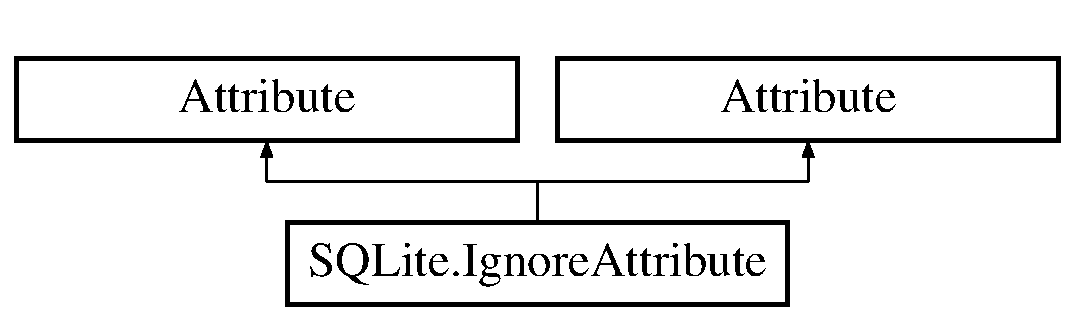
\includegraphics[height=2.000000cm]{classSQLite_1_1IgnoreAttribute}
\end{center}
\end{figure}


The documentation for this class was generated from the following file\-:\begin{DoxyCompactItemize}
\item 
packages/sqlite-\/net.\-1.\-0.\-8/content/S\-Q\-Lite.\-cs\end{DoxyCompactItemize}

\hypertarget{classSQLite_1_1IndexedAttribute}{}\section{S\+Q\+Lite.\+Indexed\+Attribute Class Reference}
\label{classSQLite_1_1IndexedAttribute}\index{S\+Q\+Lite.\+Indexed\+Attribute@{S\+Q\+Lite.\+Indexed\+Attribute}}
Inheritance diagram for S\+Q\+Lite.\+Indexed\+Attribute\+:\begin{figure}[H]
\begin{center}
\leavevmode
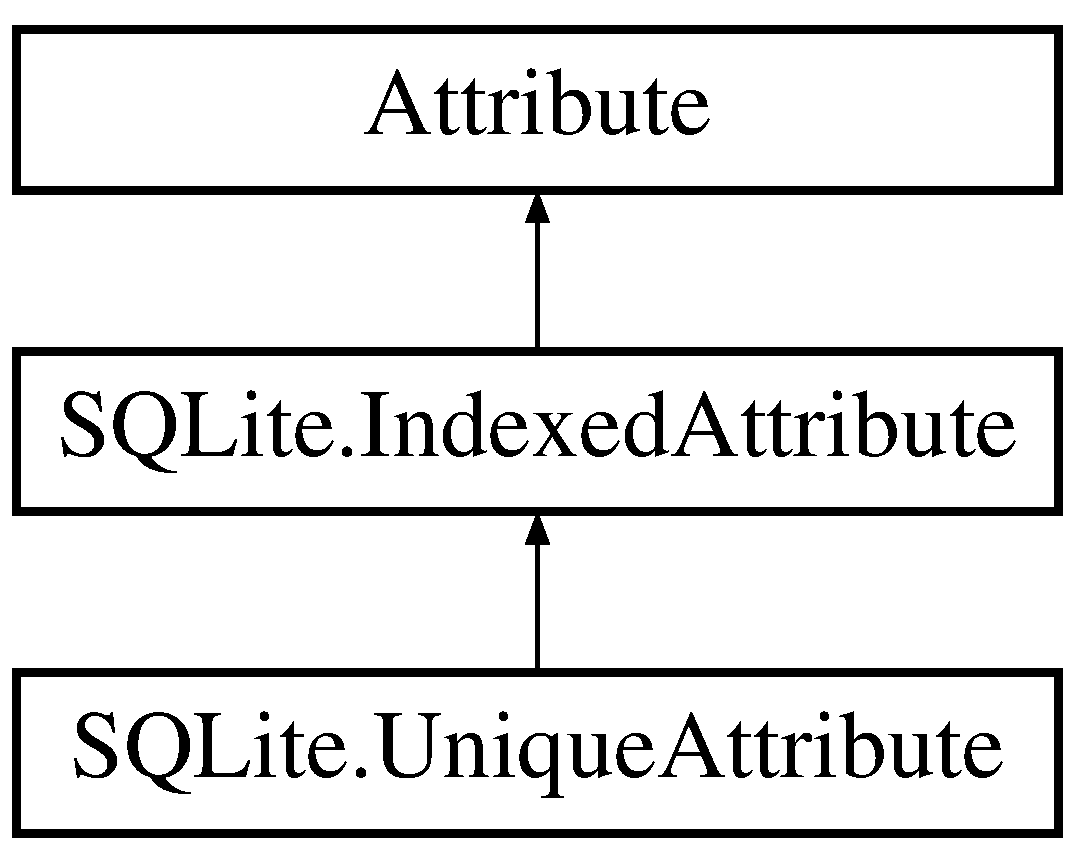
\includegraphics[height=3.000000cm]{classSQLite_1_1IndexedAttribute}
\end{center}
\end{figure}
\subsection*{Public Member Functions}
\begin{DoxyCompactItemize}
\item 
\hypertarget{classSQLite_1_1IndexedAttribute_a6d43155fc211d6c76d27326c66c39752}{}{\bfseries Indexed\+Attribute} (string name, int order)\label{classSQLite_1_1IndexedAttribute_a6d43155fc211d6c76d27326c66c39752}

\end{DoxyCompactItemize}
\subsection*{Properties}
\begin{DoxyCompactItemize}
\item 
\hypertarget{classSQLite_1_1IndexedAttribute_a55689d97d0aca7c218c9677b2ddf2dd0}{}string {\bfseries Name}\hspace{0.3cm}{\ttfamily  \mbox{[}get, set\mbox{]}}\label{classSQLite_1_1IndexedAttribute_a55689d97d0aca7c218c9677b2ddf2dd0}

\item 
\hypertarget{classSQLite_1_1IndexedAttribute_a5d6a42950339c3ae6060c1065467277a}{}int {\bfseries Order}\hspace{0.3cm}{\ttfamily  \mbox{[}get, set\mbox{]}}\label{classSQLite_1_1IndexedAttribute_a5d6a42950339c3ae6060c1065467277a}

\item 
\hypertarget{classSQLite_1_1IndexedAttribute_a081cfea90b6aba263fb1b02c4897638a}{}virtual bool {\bfseries Unique}\hspace{0.3cm}{\ttfamily  \mbox{[}get, set\mbox{]}}\label{classSQLite_1_1IndexedAttribute_a081cfea90b6aba263fb1b02c4897638a}

\end{DoxyCompactItemize}


The documentation for this class was generated from the following file\+:\begin{DoxyCompactItemize}
\item 
packages/sqlite-\/net.\+1.\+0.\+8/content/S\+Q\+Lite.\+cs\end{DoxyCompactItemize}

\hypertarget{classCore_1_1Models_1_1LatLon}{}\section{Core.\+Models.\+Lat\+Lon Class Reference}
\label{classCore_1_1Models_1_1LatLon}\index{Core.\+Models.\+Lat\+Lon@{Core.\+Models.\+Lat\+Lon}}


Latitude and Longitude of the real world.  


\subsection*{Public Member Functions}
\begin{DoxyCompactItemize}
\item 
\hyperlink{classCore_1_1Models_1_1LatLon_a5f0b81d9ee32d5df7001076a186db0ba}{Lat\+Lon} (double lat, double lon)
\begin{DoxyCompactList}\small\item\em Initializes a new instance of the \hyperlink{classCore_1_1Models_1_1LatLon}{Core.\+Models.\+Lat\+Lon} class. Latitude/\+Longitude \hyperlink{classCore_1_1Models_1_1Position}{Position} of earth. \end{DoxyCompactList}\item 
\hyperlink{classCore_1_1Models_1_1LatLon_a61ef0fd0335e0942d600ef80b7f0fcce}{Lat\+Lon} (\hyperlink{classCore_1_1Models_1_1Position}{Position} position)
\begin{DoxyCompactList}\small\item\em Initializes a new instance of the \hyperlink{classCore_1_1Models_1_1LatLon}{Core.\+Models.\+Lat\+Lon} class. \end{DoxyCompactList}\end{DoxyCompactItemize}
\subsection*{Properties}
\begin{DoxyCompactItemize}
\item 
double \hyperlink{classCore_1_1Models_1_1LatLon_a3b195e6b2a2f11d19ff283e921343638}{Lat}\hspace{0.3cm}{\ttfamily  \mbox{[}get\mbox{]}}
\begin{DoxyCompactList}\small\item\em Gets the latitude \end{DoxyCompactList}\item 
double \hyperlink{classCore_1_1Models_1_1LatLon_af16c7196d72b996c3b7f593f9ea174f1}{Lon}\hspace{0.3cm}{\ttfamily  \mbox{[}get\mbox{]}}
\begin{DoxyCompactList}\small\item\em Gets the longitude. \end{DoxyCompactList}\end{DoxyCompactItemize}


\subsection{Detailed Description}
Latitude and Longitude of the real world. 



\subsection{Constructor \& Destructor Documentation}
\hypertarget{classCore_1_1Models_1_1LatLon_a5f0b81d9ee32d5df7001076a186db0ba}{}\index{Core\+::\+Models\+::\+Lat\+Lon@{Core\+::\+Models\+::\+Lat\+Lon}!Lat\+Lon@{Lat\+Lon}}
\index{Lat\+Lon@{Lat\+Lon}!Core\+::\+Models\+::\+Lat\+Lon@{Core\+::\+Models\+::\+Lat\+Lon}}
\subsubsection[{Lat\+Lon(double lat, double lon)}]{\setlength{\rightskip}{0pt plus 5cm}Core.\+Models.\+Lat\+Lon.\+Lat\+Lon (
\begin{DoxyParamCaption}
\item[{double}]{lat, }
\item[{double}]{lon}
\end{DoxyParamCaption}
)}\label{classCore_1_1Models_1_1LatLon_a5f0b81d9ee32d5df7001076a186db0ba}


Initializes a new instance of the \hyperlink{classCore_1_1Models_1_1LatLon}{Core.\+Models.\+Lat\+Lon} class. Latitude/\+Longitude \hyperlink{classCore_1_1Models_1_1Position}{Position} of earth. 


\begin{DoxyParams}{Parameters}
{\em lat} & Latitude of earth\\
\hline
{\em lon} & Longitude of earth\\
\hline
\end{DoxyParams}
\hypertarget{classCore_1_1Models_1_1LatLon_a61ef0fd0335e0942d600ef80b7f0fcce}{}\index{Core\+::\+Models\+::\+Lat\+Lon@{Core\+::\+Models\+::\+Lat\+Lon}!Lat\+Lon@{Lat\+Lon}}
\index{Lat\+Lon@{Lat\+Lon}!Core\+::\+Models\+::\+Lat\+Lon@{Core\+::\+Models\+::\+Lat\+Lon}}
\subsubsection[{Lat\+Lon(\+Position position)}]{\setlength{\rightskip}{0pt plus 5cm}Core.\+Models.\+Lat\+Lon.\+Lat\+Lon (
\begin{DoxyParamCaption}
\item[{{\bf Position}}]{position}
\end{DoxyParamCaption}
)}\label{classCore_1_1Models_1_1LatLon_a61ef0fd0335e0942d600ef80b7f0fcce}


Initializes a new instance of the \hyperlink{classCore_1_1Models_1_1LatLon}{Core.\+Models.\+Lat\+Lon} class. 


\begin{DoxyParams}{Parameters}
{\em position} & \hyperlink{classCore_1_1Models_1_1Position}{Position} which should be converted to a \hyperlink{classCore_1_1Models_1_1LatLon}{Core.\+Models.\+Lat\+Lon} \hyperlink{classCore_1_1Models_1_1Position}{Position}.\\
\hline
\end{DoxyParams}


\subsection{Property Documentation}
\hypertarget{classCore_1_1Models_1_1LatLon_a3b195e6b2a2f11d19ff283e921343638}{}\index{Core\+::\+Models\+::\+Lat\+Lon@{Core\+::\+Models\+::\+Lat\+Lon}!Lat@{Lat}}
\index{Lat@{Lat}!Core\+::\+Models\+::\+Lat\+Lon@{Core\+::\+Models\+::\+Lat\+Lon}}
\subsubsection[{Lat}]{\setlength{\rightskip}{0pt plus 5cm}double Core.\+Models.\+Lat\+Lon.\+Lat\hspace{0.3cm}{\ttfamily [get]}}\label{classCore_1_1Models_1_1LatLon_a3b195e6b2a2f11d19ff283e921343638}


Gets the latitude 

The latitude.\hypertarget{classCore_1_1Models_1_1LatLon_af16c7196d72b996c3b7f593f9ea174f1}{}\index{Core\+::\+Models\+::\+Lat\+Lon@{Core\+::\+Models\+::\+Lat\+Lon}!Lon@{Lon}}
\index{Lon@{Lon}!Core\+::\+Models\+::\+Lat\+Lon@{Core\+::\+Models\+::\+Lat\+Lon}}
\subsubsection[{Lon}]{\setlength{\rightskip}{0pt plus 5cm}double Core.\+Models.\+Lat\+Lon.\+Lon\hspace{0.3cm}{\ttfamily [get]}}\label{classCore_1_1Models_1_1LatLon_af16c7196d72b996c3b7f593f9ea174f1}


Gets the longitude. 

The longitude.

The documentation for this class was generated from the following file\+:\begin{DoxyCompactItemize}
\item 
base/\+Models/\+Position/Lat\+Lon.\+cs\end{DoxyCompactItemize}

\hypertarget{classclient_1_1Droid_1_1Resource_1_1Layout}{\section{client.\-Droid.\-Resource.\-Layout Class Reference}
\label{classclient_1_1Droid_1_1Resource_1_1Layout}\index{client.\-Droid.\-Resource.\-Layout@{client.\-Droid.\-Resource.\-Layout}}
}
\subsection*{Public Attributes}
\begin{DoxyCompactItemize}
\item 
\hypertarget{classclient_1_1Droid_1_1Resource_1_1Layout_af8fc52c3022e4e69f71edb40b1a87aa7}{const int {\bfseries calendar\-\_\-pager\-\_\-layout} = 2130903040}\label{classclient_1_1Droid_1_1Resource_1_1Layout_af8fc52c3022e4e69f71edb40b1a87aa7}

\item 
\hypertarget{classclient_1_1Droid_1_1Resource_1_1Layout_ac1eb8be0fd7c4eb03580600fe48793c4}{const int {\bfseries calendar\-\_\-picker} = 2130903041}\label{classclient_1_1Droid_1_1Resource_1_1Layout_ac1eb8be0fd7c4eb03580600fe48793c4}

\item 
\hypertarget{classclient_1_1Droid_1_1Resource_1_1Layout_a34cd4a30c8460217cdf0f25e4198daf1}{const int {\bfseries dialog} = 2130903042}\label{classclient_1_1Droid_1_1Resource_1_1Layout_a34cd4a30c8460217cdf0f25e4198daf1}

\item 
\hypertarget{classclient_1_1Droid_1_1Resource_1_1Layout_ae2c17f1d0e71a936b9fa5ee33685ffe7}{const int {\bfseries month} = 2130903043}\label{classclient_1_1Droid_1_1Resource_1_1Layout_ae2c17f1d0e71a936b9fa5ee33685ffe7}

\item 
\hypertarget{classclient_1_1Droid_1_1Resource_1_1Layout_afebfc2611ecc130e8eaa7b227d0c97f3}{const int {\bfseries week} = 2130903044}\label{classclient_1_1Droid_1_1Resource_1_1Layout_afebfc2611ecc130e8eaa7b227d0c97f3}

\end{DoxyCompactItemize}


The documentation for this class was generated from the following file\-:\begin{DoxyCompactItemize}
\item 
client/client/client.\-Android/\-Resources/Resource.\-designer.\-cs\end{DoxyCompactItemize}

\hypertarget{classCore_1_1Helper_1_1LoadHelper}{}\section{Core.\+Helper.\+Load\+Helper Class Reference}
\label{classCore_1_1Helper_1_1LoadHelper}\index{Core.\+Helper.\+Load\+Helper@{Core.\+Helper.\+Load\+Helper}}


\hyperlink{namespaceCore_1_1Helper}{Helper}, used to load a region.  


\subsection*{Static Public Member Functions}
\begin{DoxyCompactItemize}
\item 
static string \hyperlink{classCore_1_1Helper_1_1LoadHelper_a640d07c856bb1e1b8e8e17666c9cadea}{Replace\+Path} (string path, \hyperlink{classCore_1_1Models_1_1RegionPosition}{Core.\+Models.\+Region\+Position} region\+Position)
\begin{DoxyCompactList}\small\item\em Replaces parts of the path with Major\+Region and Minor\+Region of the given Region Position \end{DoxyCompactList}\item 
static \hyperlink{classCore_1_1Models_1_1Definitions_1_1TerrainDefinition}{Core.\+Models.\+Definitions.\+Terrain\+Definition}\mbox{[},\mbox{]} \hyperlink{classCore_1_1Helper_1_1LoadHelper_a6f20b66dcc8ab52e25f09d0cdc7ebfcd}{Json\+To\+Terrain} (string json)
\begin{DoxyCompactList}\small\item\em Converts J\+S\+O\+N to an Terrain\+Definition\mbox{[} , \mbox{]} \end{DoxyCompactList}\item 
static \hyperlink{classCore_1_1Models_1_1Region}{Core.\+Models.\+Region} \hyperlink{classCore_1_1Helper_1_1LoadHelper_ace39477d290680fce596cf46869b92b6}{Json\+To\+Region} (string json, \hyperlink{classCore_1_1Models_1_1RegionPosition}{Core.\+Models.\+Region\+Position} region\+Position)
\begin{DoxyCompactList}\small\item\em Converts a J\+S\+O\+N String to a Region. \end{DoxyCompactList}\end{DoxyCompactItemize}


\subsection{Detailed Description}
\hyperlink{namespaceCore_1_1Helper}{Helper}, used to load a region. 



\subsection{Member Function Documentation}
\hypertarget{classCore_1_1Helper_1_1LoadHelper_ace39477d290680fce596cf46869b92b6}{}\index{Core\+::\+Helper\+::\+Load\+Helper@{Core\+::\+Helper\+::\+Load\+Helper}!Json\+To\+Region@{Json\+To\+Region}}
\index{Json\+To\+Region@{Json\+To\+Region}!Core\+::\+Helper\+::\+Load\+Helper@{Core\+::\+Helper\+::\+Load\+Helper}}
\subsubsection[{Json\+To\+Region(string json, Core.\+Models.\+Region\+Position region\+Position)}]{\setlength{\rightskip}{0pt plus 5cm}static {\bf Core.\+Models.\+Region} Core.\+Helper.\+Load\+Helper.\+Json\+To\+Region (
\begin{DoxyParamCaption}
\item[{string}]{json, }
\item[{{\bf Core.\+Models.\+Region\+Position}}]{region\+Position}
\end{DoxyParamCaption}
)\hspace{0.3cm}{\ttfamily [static]}}\label{classCore_1_1Helper_1_1LoadHelper_ace39477d290680fce596cf46869b92b6}


Converts a J\+S\+O\+N String to a Region. 

\begin{DoxyReturn}{Returns}
Region which was created by the J\+S\+O\+N String.
\end{DoxyReturn}

\begin{DoxyParams}{Parameters}
{\em json} & J\+S\+O\+N loaded from the server\\
\hline
{\em region\+Position} & Region position.\\
\hline
\end{DoxyParams}
\hypertarget{classCore_1_1Helper_1_1LoadHelper_a6f20b66dcc8ab52e25f09d0cdc7ebfcd}{}\index{Core\+::\+Helper\+::\+Load\+Helper@{Core\+::\+Helper\+::\+Load\+Helper}!Json\+To\+Terrain@{Json\+To\+Terrain}}
\index{Json\+To\+Terrain@{Json\+To\+Terrain}!Core\+::\+Helper\+::\+Load\+Helper@{Core\+::\+Helper\+::\+Load\+Helper}}
\subsubsection[{Json\+To\+Terrain(string json)}]{\setlength{\rightskip}{0pt plus 5cm}static {\bf Core.\+Models.\+Definitions.\+Terrain\+Definition} \mbox{[},\mbox{]} Core.\+Helper.\+Load\+Helper.\+Json\+To\+Terrain (
\begin{DoxyParamCaption}
\item[{string}]{json}
\end{DoxyParamCaption}
)\hspace{0.3cm}{\ttfamily [static]}}\label{classCore_1_1Helper_1_1LoadHelper_a6f20b66dcc8ab52e25f09d0cdc7ebfcd}


Converts J\+S\+O\+N to an Terrain\+Definition\mbox{[} , \mbox{]} 

\begin{DoxyReturn}{Returns}
A two-\/dimensional array of Terrain\+Definitions
\end{DoxyReturn}

\begin{DoxyParams}{Parameters}
{\em json} & J\+S\+O\+N loaded from the server\\
\hline
\end{DoxyParams}
\hypertarget{classCore_1_1Helper_1_1LoadHelper_a640d07c856bb1e1b8e8e17666c9cadea}{}\index{Core\+::\+Helper\+::\+Load\+Helper@{Core\+::\+Helper\+::\+Load\+Helper}!Replace\+Path@{Replace\+Path}}
\index{Replace\+Path@{Replace\+Path}!Core\+::\+Helper\+::\+Load\+Helper@{Core\+::\+Helper\+::\+Load\+Helper}}
\subsubsection[{Replace\+Path(string path, Core.\+Models.\+Region\+Position region\+Position)}]{\setlength{\rightskip}{0pt plus 5cm}static string Core.\+Helper.\+Load\+Helper.\+Replace\+Path (
\begin{DoxyParamCaption}
\item[{string}]{path, }
\item[{{\bf Core.\+Models.\+Region\+Position}}]{region\+Position}
\end{DoxyParamCaption}
)\hspace{0.3cm}{\ttfamily [static]}}\label{classCore_1_1Helper_1_1LoadHelper_a640d07c856bb1e1b8e8e17666c9cadea}


Replaces parts of the path with Major\+Region and Minor\+Region of the given Region Position 

\begin{DoxyReturn}{Returns}
Path with replaced \$\+Major\+Region and \$\+Minor\+Region 
\end{DoxyReturn}

\begin{DoxyParams}{Parameters}
{\em path} & Template Path\\
\hline
{\em region\+Position} & Region Position.\\
\hline
\end{DoxyParams}


The documentation for this class was generated from the following file\+:\begin{DoxyCompactItemize}
\item 
base/\+Helper/Load\+Helper.\+cs\end{DoxyCompactItemize}

\hypertarget{classCore_1_1Connections_1_1LoadRegionsRequest}{\section{Core.\-Connections.\-Load\-Regions\-Request Class Reference}
\label{classCore_1_1Connections_1_1LoadRegionsRequest}\index{Core.\-Connections.\-Load\-Regions\-Request@{Core.\-Connections.\-Load\-Regions\-Request}}
}


\hyperlink{classCore_1_1Connections_1_1Request}{Request} class which should be used to load regions from the server. Should be serialised before sending, will be deserialised after recieving.  


Inheritance diagram for Core.\-Connections.\-Load\-Regions\-Request\-:\begin{figure}[H]
\begin{center}
\leavevmode
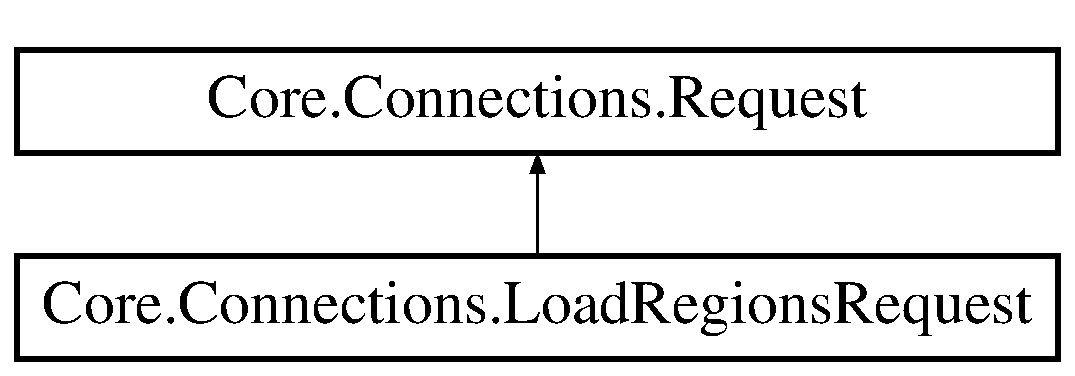
\includegraphics[height=2.000000cm]{classCore_1_1Connections_1_1LoadRegionsRequest}
\end{center}
\end{figure}
\subsection*{Public Member Functions}
\begin{DoxyCompactItemize}
\item 
\hypertarget{classCore_1_1Connections_1_1LoadRegionsRequest_ac0cb2eee50164cbd2449536ecb29956a}{{\bfseries Load\-Regions\-Request} (Guid session\-I\-D, \hyperlink{classCore_1_1Models_1_1Position}{Core.\-Models.\-Position} position, \hyperlink{classCore_1_1Models_1_1RegionPosition}{Core.\-Models.\-Region\-Position}\mbox{[}$\,$\mbox{]} region\-Positions)}\label{classCore_1_1Connections_1_1LoadRegionsRequest_ac0cb2eee50164cbd2449536ecb29956a}

\end{DoxyCompactItemize}
\subsection*{Properties}
\begin{DoxyCompactItemize}
\item 
\hypertarget{classCore_1_1Connections_1_1LoadRegionsRequest_a218b8fc9a7dc007031abe6344dc3dc64}{\hyperlink{classCore_1_1Models_1_1RegionPosition}{Core.\-Models.\-Region\-Position}\mbox{[}$\,$\mbox{]} {\bfseries Region\-Positions}\hspace{0.3cm}{\ttfamily  \mbox{[}get, set\mbox{]}}}\label{classCore_1_1Connections_1_1LoadRegionsRequest_a218b8fc9a7dc007031abe6344dc3dc64}

\end{DoxyCompactItemize}
\subsection*{Additional Inherited Members}


\subsection{Detailed Description}
\hyperlink{classCore_1_1Connections_1_1Request}{Request} class which should be used to load regions from the server. Should be serialised before sending, will be deserialised after recieving. 



The documentation for this class was generated from the following file\-:\begin{DoxyCompactItemize}
\item 
base/\-Connection/Load\-Regions\-Request.\-cs\end{DoxyCompactItemize}

\hypertarget{classCore_1_1Models_1_1LogicRules}{}\section{Core.\+Models.\+Logic\+Rules Class Reference}
\label{classCore_1_1Models_1_1LogicRules}\index{Core.\+Models.\+Logic\+Rules@{Core.\+Models.\+Logic\+Rules}}


Logic rules.  


\subsection*{Static Public Member Functions}
\begin{DoxyCompactItemize}
\item 
static int \hyperlink{classCore_1_1Models_1_1LogicRules_a81fbf661595253620a63091f139e78e8}{Ranged\+In\+Meele\+Malus} (\hyperlink{classCore_1_1Models_1_1Entity}{Entity} entity)
\begin{DoxyCompactList}\small\item\em The ranged in melee minus point. \end{DoxyCompactList}\item 
static I\+List \hyperlink{classCore_1_1Models_1_1LogicRules_a6f32bcf0c8d5d0de815beb46dd8e5051}{All\+Attack\+Modifier} (\hyperlink{classCore_1_1Models_1_1Entity}{Entity} entity)
\begin{DoxyCompactList}\small\item\em All the attack modifier. \end{DoxyCompactList}\item 
static I\+List \hyperlink{classCore_1_1Models_1_1LogicRules_a839324078b8c500d9f0904aed9f2a896}{All\+Attack\+Modifier\+Ranged\+In\+Meele} (\hyperlink{classCore_1_1Models_1_1Entity}{Entity} entity)
\begin{DoxyCompactList}\small\item\em All the attack modifier. \end{DoxyCompactList}\item 
static I\+List \hyperlink{classCore_1_1Models_1_1LogicRules_a24a0497c12320f232a258db77045ea03}{All\+Defense\+Modifier} (\hyperlink{classCore_1_1Models_1_1Entity}{Entity} entity)
\begin{DoxyCompactList}\small\item\em All the defense modifier. \end{DoxyCompactList}\item 
static \hyperlink{classCore_1_1Models_1_1PositionI}{Position\+I}\mbox{[}$\,$\mbox{]} \hyperlink{classCore_1_1Models_1_1LogicRules_a27e2ffeb0da34f1119908281fc5a6510}{Get\+Surrounded\+Fields} (\hyperlink{classCore_1_1Models_1_1PositionI}{Position\+I} pos)
\begin{DoxyCompactList}\small\item\em Gets the surrounded fields. \end{DoxyCompactList}\item 
static Hash\+Set$<$ \hyperlink{classCore_1_1Models_1_1PositionI}{Position\+I} $>$ \hyperlink{classCore_1_1Models_1_1LogicRules_acbb757cd665530aeb298e4a467051ae8}{Get\+Surrounded\+Positions} (\hyperlink{classCore_1_1Models_1_1PositionI}{Position\+I} entity, int range)
\begin{DoxyCompactList}\small\item\em Gets the surrounded territory around a given \hyperlink{classCore_1_1Models_1_1Position}{Position}. \end{DoxyCompactList}\item 
static int \hyperlink{classCore_1_1Models_1_1LogicRules_a97d3cb9e89712688aadd9a55c33b1131}{Dice} (\hyperlink{classCore_1_1Models_1_1Entity}{Entity} entity)
\begin{DoxyCompactList}\small\item\em Dice the specified attack damage for the entity. \end{DoxyCompactList}\item 
static int \hyperlink{classCore_1_1Models_1_1LogicRules_afb1653a247c550abefe670ca433e0ea2}{Terrain\+Defense\+Modifier} (\hyperlink{classCore_1_1Models_1_1Entity}{Entity} entity)
\begin{DoxyCompactList}\small\item\em Terrain for the defense modifier. \end{DoxyCompactList}\item 
static int \hyperlink{classCore_1_1Models_1_1LogicRules_aa4b7023024d0ec1bff7671f7175fa748}{Terrain\+Attack\+Modifier} (\hyperlink{classCore_1_1Models_1_1Entity}{Entity} entity)
\begin{DoxyCompactList}\small\item\em Terrain terrain for the attack modifier. \end{DoxyCompactList}\item 
static List$<$ long $>$ \hyperlink{classCore_1_1Models_1_1LogicRules_ad57cefd425a49ecd97447217eddeeadd}{Enable\+Headquarter\+Build\+Options} ()
\begin{DoxyCompactList}\small\item\em Enables the headquarter build options headquarter = 276. \end{DoxyCompactList}\item 
static List$<$ long $>$ \hyperlink{classCore_1_1Models_1_1LogicRules_ad990bb1ba29df6cc6236d7264d598822}{Enable\+Barracks\+Build\+Options} ()
\begin{DoxyCompactList}\small\item\em Enables the barracks build options barracks = 282. \end{DoxyCompactList}\item 
static void \hyperlink{classCore_1_1Models_1_1LogicRules_a16f9b1582af4ca59ac7d13044291b0bf}{Enable\+Build\+Options} (long entity\+Type, \hyperlink{classCore_1_1Models_1_1Account}{Account} account)
\begin{DoxyCompactList}\small\item\em Enables the build options. \end{DoxyCompactList}\item 
static void \hyperlink{classCore_1_1Models_1_1LogicRules_a6a1f94c43009b7a9238388281ffbadf7}{Disable\+Build\+Options} (long entity\+Type, \hyperlink{classCore_1_1Models_1_1Account}{Account} account)
\begin{DoxyCompactList}\small\item\em Disables the build options. \end{DoxyCompactList}\item 
static void \hyperlink{classCore_1_1Models_1_1LogicRules_a067a223a3eb6d870b2d05448d9967a22}{Increase\+Whole\+Storage} (\hyperlink{classCore_1_1Models_1_1Account}{Account} account)
\begin{DoxyCompactList}\small\item\em Increases the hole storage. \end{DoxyCompactList}\item 
static void \hyperlink{classCore_1_1Models_1_1LogicRules_af7b01bd5aae498990758b6e08542781f}{Decrease\+Whole\+Storage} (\hyperlink{classCore_1_1Models_1_1Account}{Account} account)
\begin{DoxyCompactList}\small\item\em Decreases the hole storage. \end{DoxyCompactList}\item 
static void \hyperlink{classCore_1_1Models_1_1LogicRules_ab9e45f139a56d49c34db56e9cf5b1e4c}{Increase\+Max\+Population} (\hyperlink{classCore_1_1Models_1_1Account}{Account} account, \hyperlink{classCore_1_1Models_1_1Entity}{Entity} entity)
\begin{DoxyCompactList}\small\item\em Increases the population. \end{DoxyCompactList}\item 
static void \hyperlink{classCore_1_1Models_1_1LogicRules_ab15c9eee68f915382f717968fe107d01}{Increase\+Max\+Energy} (\hyperlink{classCore_1_1Models_1_1Account}{Account} account, \hyperlink{classCore_1_1Models_1_1Entity}{Entity} entity)
\begin{DoxyCompactList}\small\item\em Increases the max energy. \end{DoxyCompactList}\item 
static void \hyperlink{classCore_1_1Models_1_1LogicRules_a2bf267a445128ca26bd61c8113fad7df}{Set\+Current\+Max\+Population} (\hyperlink{classCore_1_1Models_1_1Account}{Account} account)
\begin{DoxyCompactList}\small\item\em Sets the current max population. \end{DoxyCompactList}\item 
static void \hyperlink{classCore_1_1Models_1_1LogicRules_ac890759359d9ea01c51d423dbe504e89}{Set\+Current\+Max\+Energy} (\hyperlink{classCore_1_1Models_1_1Account}{Account} account)
\begin{DoxyCompactList}\small\item\em Sets the current energy. \end{DoxyCompactList}\item 
static void \hyperlink{classCore_1_1Models_1_1LogicRules_a012d1303c1d681129fd1df10b9ac194c}{Increase\+Scrap} (\hyperlink{classCore_1_1Models_1_1Account}{Account} account, \hyperlink{classCore_1_1Models_1_1Entity}{Entity} entity)
\begin{DoxyCompactList}\small\item\em Increases the scrap. \end{DoxyCompactList}\item 
static void \hyperlink{classCore_1_1Models_1_1LogicRules_affe9e8724caf3ef5b5d8c7e2d992d389}{Decrease\+Max\+Population} (\hyperlink{classCore_1_1Models_1_1Account}{Account} account, \hyperlink{classCore_1_1Models_1_1Entity}{Entity} entity)
\begin{DoxyCompactList}\small\item\em Decreases the population. \end{DoxyCompactList}\item 
static void \hyperlink{classCore_1_1Models_1_1LogicRules_a25f86390ccb398e269122da226220cef}{Decrease\+Max\+Energy} (\hyperlink{classCore_1_1Models_1_1Account}{Account} account, \hyperlink{classCore_1_1Models_1_1Entity}{Entity} entity)
\begin{DoxyCompactList}\small\item\em Decreases the max energy. \end{DoxyCompactList}\item 
static void \hyperlink{classCore_1_1Models_1_1LogicRules_a5ebbe4ae42aeef6b5774882e89a5ccb4}{Decrease\+Scrap} (\hyperlink{classCore_1_1Models_1_1Account}{Account} account, \hyperlink{classCore_1_1Models_1_1Entity}{Entity} entity)
\begin{DoxyCompactList}\small\item\em Decreases the population. \end{DoxyCompactList}\item 
static void \hyperlink{classCore_1_1Models_1_1LogicRules_ae7859acf93d2dd6153b1d7490a76bec6}{Increase\+Storage} (\hyperlink{classCore_1_1Models_1_1Account}{Account} account, \hyperlink{classCore_1_1Models_1_1Entity}{Entity} entity)
\begin{DoxyCompactList}\small\item\em Increases the storage. \end{DoxyCompactList}\item 
static void \hyperlink{classCore_1_1Models_1_1LogicRules_a61386300d32614e241e31457ef2395ef}{Decreas\+Storage} (\hyperlink{classCore_1_1Models_1_1Account}{Account} account, \hyperlink{classCore_1_1Models_1_1Entity}{Entity} entity)
\begin{DoxyCompactList}\small\item\em Decreases the storage. \end{DoxyCompactList}\item 
static void \hyperlink{classCore_1_1Models_1_1LogicRules_ab775894692c4712e0e1920380ee9de07}{Gather\+Resources} (\hyperlink{classCore_1_1Models_1_1Account}{Account} account, Date\+Time action\+Time, \hyperlink{classCore_1_1Controllers_1_1RegionManagerController}{Controllers.\+Region\+Manager\+Controller} region\+Manager\+C, int range)
\begin{DoxyCompactList}\small\item\em Gathers the resources. \end{DoxyCompactList}\item 
static void \hyperlink{classCore_1_1Models_1_1LogicRules_a8108a7426fbef7689f4b3cec1492e6cb}{Increase\+Resource\+Generation} (\hyperlink{classCore_1_1Models_1_1Account}{Account} account, Date\+Time action\+Time, \hyperlink{classCore_1_1Models_1_1PositionI}{Position\+I} entitypos, \hyperlink{classCore_1_1Controllers_1_1RegionManagerController}{Controllers.\+Region\+Manager\+Controller} region\+Manager\+C)
\begin{DoxyCompactList}\small\item\em Increases the resource generation. \end{DoxyCompactList}\item 
static void \hyperlink{classCore_1_1Models_1_1LogicRules_afdd4a1980e815cee411b0cf5fff0427d}{Decrease\+Resource\+Generation} (\hyperlink{classCore_1_1Models_1_1Account}{Account} account, Date\+Time action\+Time, \hyperlink{classCore_1_1Models_1_1PositionI}{Position\+I} entitypos, \hyperlink{classCore_1_1Controllers_1_1RegionManagerController}{Controllers.\+Region\+Manager\+Controller} region\+Manager\+C)
\begin{DoxyCompactList}\small\item\em Decreases the resource generation. \end{DoxyCompactList}\item 
static bool \hyperlink{classCore_1_1Models_1_1LogicRules_ae686cefdb61e6caee8bc0dee09ee71f3}{Check\+Resource} (\hyperlink{classCore_1_1Models_1_1Account}{Account} account, Date\+Time server\+Time, \hyperlink{classCore_1_1Models_1_1Definitions_1_1Definition}{Definitions.\+Definition} entity\+Def)
\begin{DoxyCompactList}\small\item\em Checks the resource cost of the entity. \end{DoxyCompactList}\item 
static void \hyperlink{classCore_1_1Models_1_1LogicRules_ad3b250727f8358799fc881cb0c00644d}{Consume\+Resource} (\hyperlink{classCore_1_1Models_1_1Account}{Account} account, Date\+Time action\+Time, \hyperlink{classCore_1_1Models_1_1Definitions_1_1Definition}{Definitions.\+Definition} entity\+Def)
\begin{DoxyCompactList}\small\item\em Consumes the resource for an entity. \end{DoxyCompactList}\item 
static void \hyperlink{classCore_1_1Models_1_1LogicRules_aa71e5341064abab193e8cb472d4e906f}{Destroy\+Building} (\hyperlink{classCore_1_1Models_1_1Entity}{Entity} entity, \hyperlink{classCore_1_1Models_1_1Region}{Region} region\+Pos, \hyperlink{classCore_1_1Models_1_1Action}{Action} action, \hyperlink{classCore_1_1Controllers_1_1RegionManagerController}{Controllers.\+Region\+Manager\+Controller} region\+Manager\+C)
\begin{DoxyCompactList}\small\item\em Destroy the building and undo the functionality. \end{DoxyCompactList}\item 
static void \hyperlink{classCore_1_1Models_1_1LogicRules_a7139405da4b52991042628844749b791}{Destroy\+All\+Buildings\+Without\+Territory} (\hyperlink{classCore_1_1Models_1_1Account}{Account} account, \hyperlink{classCore_1_1Models_1_1Action}{Action} action, \hyperlink{classCore_1_1Controllers_1_1RegionManagerController}{Controllers.\+Region\+Manager\+Controller} region\+Manager\+C)
\begin{DoxyCompactList}\small\item\em Destroy all buildings without territory. \end{DoxyCompactList}\end{DoxyCompactItemize}
\subsection*{Static Public Attributes}
\begin{DoxyCompactItemize}
\item 
static readonly \hyperlink{classCore_1_1Models_1_1PositionI}{Position\+I}\mbox{[}$\,$\mbox{]} \hyperlink{classCore_1_1Models_1_1LogicRules_a3d587d8f781d3b37c26c501d003f3d4d}{Surround\+Tiles\+Even}
\begin{DoxyCompactList}\small\item\em The surround tiles on even x positions. From North to North\+East in clockwise \end{DoxyCompactList}\item 
static readonly \hyperlink{classCore_1_1Models_1_1PositionI}{Position\+I}\mbox{[}$\,$\mbox{]} \hyperlink{classCore_1_1Models_1_1LogicRules_ae559d0e04d49b4cea7874d1e7ca5a5b2}{Surround\+Tiles\+Odd}
\begin{DoxyCompactList}\small\item\em The surround tiles on odd x positions. From North to North\+East in clockwise \end{DoxyCompactList}\item 
static readonly \hyperlink{classCore_1_1Models_1_1RegionPosition}{Region\+Position}\mbox{[}$\,$\mbox{]} \hyperlink{classCore_1_1Models_1_1LogicRules_a42380b97e68c7128580776742ef94e56}{Surround\+Regions}
\begin{DoxyCompactList}\small\item\em Surrounded Regions from top left clockwise \end{DoxyCompactList}\end{DoxyCompactItemize}


\subsection{Detailed Description}
Logic rules. 



\subsection{Member Function Documentation}
\hypertarget{classCore_1_1Models_1_1LogicRules_a6f32bcf0c8d5d0de815beb46dd8e5051}{}\index{Core\+::\+Models\+::\+Logic\+Rules@{Core\+::\+Models\+::\+Logic\+Rules}!All\+Attack\+Modifier@{All\+Attack\+Modifier}}
\index{All\+Attack\+Modifier@{All\+Attack\+Modifier}!Core\+::\+Models\+::\+Logic\+Rules@{Core\+::\+Models\+::\+Logic\+Rules}}
\subsubsection[{All\+Attack\+Modifier(\+Entity entity)}]{\setlength{\rightskip}{0pt plus 5cm}static I\+List Core.\+Models.\+Logic\+Rules.\+All\+Attack\+Modifier (
\begin{DoxyParamCaption}
\item[{{\bf Entity}}]{entity}
\end{DoxyParamCaption}
)\hspace{0.3cm}{\ttfamily [static]}}\label{classCore_1_1Models_1_1LogicRules_a6f32bcf0c8d5d0de815beb46dd8e5051}


All the attack modifier. 

\begin{DoxyReturn}{Returns}
The attack modifier.
\end{DoxyReturn}

\begin{DoxyParams}{Parameters}
{\em entity} & Current \hyperlink{classCore_1_1Models_1_1Entity}{Entity}.\\
\hline
\end{DoxyParams}
\hypertarget{classCore_1_1Models_1_1LogicRules_a839324078b8c500d9f0904aed9f2a896}{}\index{Core\+::\+Models\+::\+Logic\+Rules@{Core\+::\+Models\+::\+Logic\+Rules}!All\+Attack\+Modifier\+Ranged\+In\+Meele@{All\+Attack\+Modifier\+Ranged\+In\+Meele}}
\index{All\+Attack\+Modifier\+Ranged\+In\+Meele@{All\+Attack\+Modifier\+Ranged\+In\+Meele}!Core\+::\+Models\+::\+Logic\+Rules@{Core\+::\+Models\+::\+Logic\+Rules}}
\subsubsection[{All\+Attack\+Modifier\+Ranged\+In\+Meele(\+Entity entity)}]{\setlength{\rightskip}{0pt plus 5cm}static I\+List Core.\+Models.\+Logic\+Rules.\+All\+Attack\+Modifier\+Ranged\+In\+Meele (
\begin{DoxyParamCaption}
\item[{{\bf Entity}}]{entity}
\end{DoxyParamCaption}
)\hspace{0.3cm}{\ttfamily [static]}}\label{classCore_1_1Models_1_1LogicRules_a839324078b8c500d9f0904aed9f2a896}


All the attack modifier. 

\begin{DoxyReturn}{Returns}
The attack modifier.
\end{DoxyReturn}

\begin{DoxyParams}{Parameters}
{\em entity} & Current \hyperlink{classCore_1_1Models_1_1Entity}{Entity}.\\
\hline
\end{DoxyParams}
\hypertarget{classCore_1_1Models_1_1LogicRules_a24a0497c12320f232a258db77045ea03}{}\index{Core\+::\+Models\+::\+Logic\+Rules@{Core\+::\+Models\+::\+Logic\+Rules}!All\+Defense\+Modifier@{All\+Defense\+Modifier}}
\index{All\+Defense\+Modifier@{All\+Defense\+Modifier}!Core\+::\+Models\+::\+Logic\+Rules@{Core\+::\+Models\+::\+Logic\+Rules}}
\subsubsection[{All\+Defense\+Modifier(\+Entity entity)}]{\setlength{\rightskip}{0pt plus 5cm}static I\+List Core.\+Models.\+Logic\+Rules.\+All\+Defense\+Modifier (
\begin{DoxyParamCaption}
\item[{{\bf Entity}}]{entity}
\end{DoxyParamCaption}
)\hspace{0.3cm}{\ttfamily [static]}}\label{classCore_1_1Models_1_1LogicRules_a24a0497c12320f232a258db77045ea03}


All the defense modifier. 

\begin{DoxyReturn}{Returns}
The defense modifier.
\end{DoxyReturn}

\begin{DoxyParams}{Parameters}
{\em entity} & Current \hyperlink{classCore_1_1Models_1_1Entity}{Entity}.\\
\hline
\end{DoxyParams}
\hypertarget{classCore_1_1Models_1_1LogicRules_ae686cefdb61e6caee8bc0dee09ee71f3}{}\index{Core\+::\+Models\+::\+Logic\+Rules@{Core\+::\+Models\+::\+Logic\+Rules}!Check\+Resource@{Check\+Resource}}
\index{Check\+Resource@{Check\+Resource}!Core\+::\+Models\+::\+Logic\+Rules@{Core\+::\+Models\+::\+Logic\+Rules}}
\subsubsection[{Check\+Resource(\+Account account, Date\+Time server\+Time, Definitions.\+Definition entity\+Def)}]{\setlength{\rightskip}{0pt plus 5cm}static bool Core.\+Models.\+Logic\+Rules.\+Check\+Resource (
\begin{DoxyParamCaption}
\item[{{\bf Account}}]{account, }
\item[{Date\+Time}]{server\+Time, }
\item[{{\bf Definitions.\+Definition}}]{entity\+Def}
\end{DoxyParamCaption}
)\hspace{0.3cm}{\ttfamily [static]}}\label{classCore_1_1Models_1_1LogicRules_ae686cefdb61e6caee8bc0dee09ee71f3}


Checks the resource cost of the entity. 

\begin{DoxyReturn}{Returns}
{\ttfamily true}, if resource was checked, {\ttfamily false} otherwise.
\end{DoxyReturn}

\begin{DoxyParams}{Parameters}
{\em account} & Current account.\\
\hline
{\em server\+Time} & \hyperlink{namespaceServer}{Server} time.\\
\hline
{\em entity\+Def} & \hyperlink{classCore_1_1Models_1_1Entity}{Entity} definition.\\
\hline
\end{DoxyParams}
\hypertarget{classCore_1_1Models_1_1LogicRules_ad3b250727f8358799fc881cb0c00644d}{}\index{Core\+::\+Models\+::\+Logic\+Rules@{Core\+::\+Models\+::\+Logic\+Rules}!Consume\+Resource@{Consume\+Resource}}
\index{Consume\+Resource@{Consume\+Resource}!Core\+::\+Models\+::\+Logic\+Rules@{Core\+::\+Models\+::\+Logic\+Rules}}
\subsubsection[{Consume\+Resource(\+Account account, Date\+Time action\+Time, Definitions.\+Definition entity\+Def)}]{\setlength{\rightskip}{0pt plus 5cm}static void Core.\+Models.\+Logic\+Rules.\+Consume\+Resource (
\begin{DoxyParamCaption}
\item[{{\bf Account}}]{account, }
\item[{Date\+Time}]{action\+Time, }
\item[{{\bf Definitions.\+Definition}}]{entity\+Def}
\end{DoxyParamCaption}
)\hspace{0.3cm}{\ttfamily [static]}}\label{classCore_1_1Models_1_1LogicRules_ad3b250727f8358799fc881cb0c00644d}


Consumes the resource for an entity. 


\begin{DoxyParams}{Parameters}
{\em account} & Current account.\\
\hline
{\em action\+Time} & \hyperlink{classCore_1_1Models_1_1Action}{Action} time.\\
\hline
{\em entity\+Def} & \hyperlink{classCore_1_1Models_1_1Entity}{Entity} definition.\\
\hline
\end{DoxyParams}
\hypertarget{classCore_1_1Models_1_1LogicRules_a25f86390ccb398e269122da226220cef}{}\index{Core\+::\+Models\+::\+Logic\+Rules@{Core\+::\+Models\+::\+Logic\+Rules}!Decrease\+Max\+Energy@{Decrease\+Max\+Energy}}
\index{Decrease\+Max\+Energy@{Decrease\+Max\+Energy}!Core\+::\+Models\+::\+Logic\+Rules@{Core\+::\+Models\+::\+Logic\+Rules}}
\subsubsection[{Decrease\+Max\+Energy(\+Account account, Entity entity)}]{\setlength{\rightskip}{0pt plus 5cm}static void Core.\+Models.\+Logic\+Rules.\+Decrease\+Max\+Energy (
\begin{DoxyParamCaption}
\item[{{\bf Account}}]{account, }
\item[{{\bf Entity}}]{entity}
\end{DoxyParamCaption}
)\hspace{0.3cm}{\ttfamily [static]}}\label{classCore_1_1Models_1_1LogicRules_a25f86390ccb398e269122da226220cef}


Decreases the max energy. 


\begin{DoxyParams}{Parameters}
{\em account} & Current account.\\
\hline
{\em entity} & Current entity.\\
\hline
\end{DoxyParams}
\hypertarget{classCore_1_1Models_1_1LogicRules_affe9e8724caf3ef5b5d8c7e2d992d389}{}\index{Core\+::\+Models\+::\+Logic\+Rules@{Core\+::\+Models\+::\+Logic\+Rules}!Decrease\+Max\+Population@{Decrease\+Max\+Population}}
\index{Decrease\+Max\+Population@{Decrease\+Max\+Population}!Core\+::\+Models\+::\+Logic\+Rules@{Core\+::\+Models\+::\+Logic\+Rules}}
\subsubsection[{Decrease\+Max\+Population(\+Account account, Entity entity)}]{\setlength{\rightskip}{0pt plus 5cm}static void Core.\+Models.\+Logic\+Rules.\+Decrease\+Max\+Population (
\begin{DoxyParamCaption}
\item[{{\bf Account}}]{account, }
\item[{{\bf Entity}}]{entity}
\end{DoxyParamCaption}
)\hspace{0.3cm}{\ttfamily [static]}}\label{classCore_1_1Models_1_1LogicRules_affe9e8724caf3ef5b5d8c7e2d992d389}


Decreases the population. 


\begin{DoxyParams}{Parameters}
{\em account} & Current account.\\
\hline
{\em entity} & Current entity.\\
\hline
\end{DoxyParams}
\hypertarget{classCore_1_1Models_1_1LogicRules_afdd4a1980e815cee411b0cf5fff0427d}{}\index{Core\+::\+Models\+::\+Logic\+Rules@{Core\+::\+Models\+::\+Logic\+Rules}!Decrease\+Resource\+Generation@{Decrease\+Resource\+Generation}}
\index{Decrease\+Resource\+Generation@{Decrease\+Resource\+Generation}!Core\+::\+Models\+::\+Logic\+Rules@{Core\+::\+Models\+::\+Logic\+Rules}}
\subsubsection[{Decrease\+Resource\+Generation(\+Account account, Date\+Time action\+Time, Position\+I entitypos, Controllers.\+Region\+Manager\+Controller region\+Manager\+C)}]{\setlength{\rightskip}{0pt plus 5cm}static void Core.\+Models.\+Logic\+Rules.\+Decrease\+Resource\+Generation (
\begin{DoxyParamCaption}
\item[{{\bf Account}}]{account, }
\item[{Date\+Time}]{action\+Time, }
\item[{{\bf Position\+I}}]{entitypos, }
\item[{{\bf Controllers.\+Region\+Manager\+Controller}}]{region\+Manager\+C}
\end{DoxyParamCaption}
)\hspace{0.3cm}{\ttfamily [static]}}\label{classCore_1_1Models_1_1LogicRules_afdd4a1980e815cee411b0cf5fff0427d}


Decreases the resource generation. 


\begin{DoxyParams}{Parameters}
{\em account} & Current account.\\
\hline
{\em action\+Time} & \hyperlink{classCore_1_1Models_1_1Action}{Action} time.\\
\hline
{\em entitypos} & \hyperlink{classCore_1_1Models_1_1Entity}{Entity} position.\\
\hline
{\em region\+Manager\+C} & \hyperlink{classCore_1_1Models_1_1Region}{Region} manager controller.\\
\hline
\end{DoxyParams}
\hypertarget{classCore_1_1Models_1_1LogicRules_a5ebbe4ae42aeef6b5774882e89a5ccb4}{}\index{Core\+::\+Models\+::\+Logic\+Rules@{Core\+::\+Models\+::\+Logic\+Rules}!Decrease\+Scrap@{Decrease\+Scrap}}
\index{Decrease\+Scrap@{Decrease\+Scrap}!Core\+::\+Models\+::\+Logic\+Rules@{Core\+::\+Models\+::\+Logic\+Rules}}
\subsubsection[{Decrease\+Scrap(\+Account account, Entity entity)}]{\setlength{\rightskip}{0pt plus 5cm}static void Core.\+Models.\+Logic\+Rules.\+Decrease\+Scrap (
\begin{DoxyParamCaption}
\item[{{\bf Account}}]{account, }
\item[{{\bf Entity}}]{entity}
\end{DoxyParamCaption}
)\hspace{0.3cm}{\ttfamily [static]}}\label{classCore_1_1Models_1_1LogicRules_a5ebbe4ae42aeef6b5774882e89a5ccb4}


Decreases the population. 


\begin{DoxyParams}{Parameters}
{\em account} & Current account.\\
\hline
{\em entity} & Current entity.\\
\hline
\end{DoxyParams}
\hypertarget{classCore_1_1Models_1_1LogicRules_af7b01bd5aae498990758b6e08542781f}{}\index{Core\+::\+Models\+::\+Logic\+Rules@{Core\+::\+Models\+::\+Logic\+Rules}!Decrease\+Whole\+Storage@{Decrease\+Whole\+Storage}}
\index{Decrease\+Whole\+Storage@{Decrease\+Whole\+Storage}!Core\+::\+Models\+::\+Logic\+Rules@{Core\+::\+Models\+::\+Logic\+Rules}}
\subsubsection[{Decrease\+Whole\+Storage(\+Account account)}]{\setlength{\rightskip}{0pt plus 5cm}static void Core.\+Models.\+Logic\+Rules.\+Decrease\+Whole\+Storage (
\begin{DoxyParamCaption}
\item[{{\bf Account}}]{account}
\end{DoxyParamCaption}
)\hspace{0.3cm}{\ttfamily [static]}}\label{classCore_1_1Models_1_1LogicRules_af7b01bd5aae498990758b6e08542781f}


Decreases the hole storage. 


\begin{DoxyParams}{Parameters}
{\em account} & Current \hyperlink{classCore_1_1Models_1_1Account}{Account}.\\
\hline
\end{DoxyParams}
\hypertarget{classCore_1_1Models_1_1LogicRules_a61386300d32614e241e31457ef2395ef}{}\index{Core\+::\+Models\+::\+Logic\+Rules@{Core\+::\+Models\+::\+Logic\+Rules}!Decreas\+Storage@{Decreas\+Storage}}
\index{Decreas\+Storage@{Decreas\+Storage}!Core\+::\+Models\+::\+Logic\+Rules@{Core\+::\+Models\+::\+Logic\+Rules}}
\subsubsection[{Decreas\+Storage(\+Account account, Entity entity)}]{\setlength{\rightskip}{0pt plus 5cm}static void Core.\+Models.\+Logic\+Rules.\+Decreas\+Storage (
\begin{DoxyParamCaption}
\item[{{\bf Account}}]{account, }
\item[{{\bf Entity}}]{entity}
\end{DoxyParamCaption}
)\hspace{0.3cm}{\ttfamily [static]}}\label{classCore_1_1Models_1_1LogicRules_a61386300d32614e241e31457ef2395ef}


Decreases the storage. 


\begin{DoxyParams}{Parameters}
{\em account} & Current account.\\
\hline
{\em entity} & Current entity.\\
\hline
\end{DoxyParams}
\hypertarget{classCore_1_1Models_1_1LogicRules_a7139405da4b52991042628844749b791}{}\index{Core\+::\+Models\+::\+Logic\+Rules@{Core\+::\+Models\+::\+Logic\+Rules}!Destroy\+All\+Buildings\+Without\+Territory@{Destroy\+All\+Buildings\+Without\+Territory}}
\index{Destroy\+All\+Buildings\+Without\+Territory@{Destroy\+All\+Buildings\+Without\+Territory}!Core\+::\+Models\+::\+Logic\+Rules@{Core\+::\+Models\+::\+Logic\+Rules}}
\subsubsection[{Destroy\+All\+Buildings\+Without\+Territory(\+Account account, Action action, Controllers.\+Region\+Manager\+Controller region\+Manager\+C)}]{\setlength{\rightskip}{0pt plus 5cm}static void Core.\+Models.\+Logic\+Rules.\+Destroy\+All\+Buildings\+Without\+Territory (
\begin{DoxyParamCaption}
\item[{{\bf Account}}]{account, }
\item[{{\bf Action}}]{action, }
\item[{{\bf Controllers.\+Region\+Manager\+Controller}}]{region\+Manager\+C}
\end{DoxyParamCaption}
)\hspace{0.3cm}{\ttfamily [static]}}\label{classCore_1_1Models_1_1LogicRules_a7139405da4b52991042628844749b791}


Destroy all buildings without territory. 


\begin{DoxyParams}{Parameters}
{\em account} & Current account.\\
\hline
{\em action} & \hyperlink{classCore_1_1Models_1_1Action}{Action} which is in use.\\
\hline
{\em region\+Manager\+C} & \hyperlink{classCore_1_1Models_1_1Region}{Region} manager controller.\\
\hline
\end{DoxyParams}
\hypertarget{classCore_1_1Models_1_1LogicRules_aa71e5341064abab193e8cb472d4e906f}{}\index{Core\+::\+Models\+::\+Logic\+Rules@{Core\+::\+Models\+::\+Logic\+Rules}!Destroy\+Building@{Destroy\+Building}}
\index{Destroy\+Building@{Destroy\+Building}!Core\+::\+Models\+::\+Logic\+Rules@{Core\+::\+Models\+::\+Logic\+Rules}}
\subsubsection[{Destroy\+Building(\+Entity entity, Region region\+Pos, Action action, Controllers.\+Region\+Manager\+Controller region\+Manager\+C)}]{\setlength{\rightskip}{0pt plus 5cm}static void Core.\+Models.\+Logic\+Rules.\+Destroy\+Building (
\begin{DoxyParamCaption}
\item[{{\bf Entity}}]{entity, }
\item[{{\bf Region}}]{region\+Pos, }
\item[{{\bf Action}}]{action, }
\item[{{\bf Controllers.\+Region\+Manager\+Controller}}]{region\+Manager\+C}
\end{DoxyParamCaption}
)\hspace{0.3cm}{\ttfamily [static]}}\label{classCore_1_1Models_1_1LogicRules_aa71e5341064abab193e8cb472d4e906f}


Destroy the building and undo the functionality. 


\begin{DoxyParams}{Parameters}
{\em entity} & Current entity.\\
\hline
{\em region\+Pos} & \hyperlink{classCore_1_1Models_1_1Region}{Region} position.\\
\hline
{\em action} & \hyperlink{classCore_1_1Models_1_1Action}{Action} which is currently done.\\
\hline
{\em region\+Manager\+C} & \hyperlink{classCore_1_1Models_1_1Region}{Region} manager controller.\\
\hline
\end{DoxyParams}
\hypertarget{classCore_1_1Models_1_1LogicRules_a97d3cb9e89712688aadd9a55c33b1131}{}\index{Core\+::\+Models\+::\+Logic\+Rules@{Core\+::\+Models\+::\+Logic\+Rules}!Dice@{Dice}}
\index{Dice@{Dice}!Core\+::\+Models\+::\+Logic\+Rules@{Core\+::\+Models\+::\+Logic\+Rules}}
\subsubsection[{Dice(\+Entity entity)}]{\setlength{\rightskip}{0pt plus 5cm}static int Core.\+Models.\+Logic\+Rules.\+Dice (
\begin{DoxyParamCaption}
\item[{{\bf Entity}}]{entity}
\end{DoxyParamCaption}
)\hspace{0.3cm}{\ttfamily [static]}}\label{classCore_1_1Models_1_1LogicRules_a97d3cb9e89712688aadd9a55c33b1131}


Dice the specified attack damage for the entity. 

\begin{DoxyReturn}{Returns}
0 instead it change the value via pointer.
\end{DoxyReturn}

\begin{DoxyParams}{Parameters}
{\em entity} & Current \hyperlink{classCore_1_1Models_1_1Entity}{Entity}.\\
\hline
\end{DoxyParams}
\hypertarget{classCore_1_1Models_1_1LogicRules_a6a1f94c43009b7a9238388281ffbadf7}{}\index{Core\+::\+Models\+::\+Logic\+Rules@{Core\+::\+Models\+::\+Logic\+Rules}!Disable\+Build\+Options@{Disable\+Build\+Options}}
\index{Disable\+Build\+Options@{Disable\+Build\+Options}!Core\+::\+Models\+::\+Logic\+Rules@{Core\+::\+Models\+::\+Logic\+Rules}}
\subsubsection[{Disable\+Build\+Options(long entity\+Type, Account account)}]{\setlength{\rightskip}{0pt plus 5cm}static void Core.\+Models.\+Logic\+Rules.\+Disable\+Build\+Options (
\begin{DoxyParamCaption}
\item[{long}]{entity\+Type, }
\item[{{\bf Account}}]{account}
\end{DoxyParamCaption}
)\hspace{0.3cm}{\ttfamily [static]}}\label{classCore_1_1Models_1_1LogicRules_a6a1f94c43009b7a9238388281ffbadf7}


Disables the build options. 


\begin{DoxyParams}{Parameters}
{\em entity\+Type} & \hyperlink{classCore_1_1Models_1_1Entity}{Entity} type.\\
\hline
{\em account} & Current account.\\
\hline
\end{DoxyParams}
\hypertarget{classCore_1_1Models_1_1LogicRules_ad990bb1ba29df6cc6236d7264d598822}{}\index{Core\+::\+Models\+::\+Logic\+Rules@{Core\+::\+Models\+::\+Logic\+Rules}!Enable\+Barracks\+Build\+Options@{Enable\+Barracks\+Build\+Options}}
\index{Enable\+Barracks\+Build\+Options@{Enable\+Barracks\+Build\+Options}!Core\+::\+Models\+::\+Logic\+Rules@{Core\+::\+Models\+::\+Logic\+Rules}}
\subsubsection[{Enable\+Barracks\+Build\+Options()}]{\setlength{\rightskip}{0pt plus 5cm}static List$<$long$>$ Core.\+Models.\+Logic\+Rules.\+Enable\+Barracks\+Build\+Options (
\begin{DoxyParamCaption}
{}
\end{DoxyParamCaption}
)\hspace{0.3cm}{\ttfamily [static]}}\label{classCore_1_1Models_1_1LogicRules_ad990bb1ba29df6cc6236d7264d598822}


Enables the barracks build options barracks = 282. 

\begin{DoxyReturn}{Returns}
The barracks build options.
\end{DoxyReturn}
\hypertarget{classCore_1_1Models_1_1LogicRules_a16f9b1582af4ca59ac7d13044291b0bf}{}\index{Core\+::\+Models\+::\+Logic\+Rules@{Core\+::\+Models\+::\+Logic\+Rules}!Enable\+Build\+Options@{Enable\+Build\+Options}}
\index{Enable\+Build\+Options@{Enable\+Build\+Options}!Core\+::\+Models\+::\+Logic\+Rules@{Core\+::\+Models\+::\+Logic\+Rules}}
\subsubsection[{Enable\+Build\+Options(long entity\+Type, Account account)}]{\setlength{\rightskip}{0pt plus 5cm}static void Core.\+Models.\+Logic\+Rules.\+Enable\+Build\+Options (
\begin{DoxyParamCaption}
\item[{long}]{entity\+Type, }
\item[{{\bf Account}}]{account}
\end{DoxyParamCaption}
)\hspace{0.3cm}{\ttfamily [static]}}\label{classCore_1_1Models_1_1LogicRules_a16f9b1582af4ca59ac7d13044291b0bf}


Enables the build options. 


\begin{DoxyParams}{Parameters}
{\em entity\+Type} & \hyperlink{classCore_1_1Models_1_1Entity}{Entity} type.\\
\hline
{\em account} & Current \hyperlink{classCore_1_1Models_1_1Account}{Account}.\\
\hline
\end{DoxyParams}
\hypertarget{classCore_1_1Models_1_1LogicRules_ad57cefd425a49ecd97447217eddeeadd}{}\index{Core\+::\+Models\+::\+Logic\+Rules@{Core\+::\+Models\+::\+Logic\+Rules}!Enable\+Headquarter\+Build\+Options@{Enable\+Headquarter\+Build\+Options}}
\index{Enable\+Headquarter\+Build\+Options@{Enable\+Headquarter\+Build\+Options}!Core\+::\+Models\+::\+Logic\+Rules@{Core\+::\+Models\+::\+Logic\+Rules}}
\subsubsection[{Enable\+Headquarter\+Build\+Options()}]{\setlength{\rightskip}{0pt plus 5cm}static List$<$long$>$ Core.\+Models.\+Logic\+Rules.\+Enable\+Headquarter\+Build\+Options (
\begin{DoxyParamCaption}
{}
\end{DoxyParamCaption}
)\hspace{0.3cm}{\ttfamily [static]}}\label{classCore_1_1Models_1_1LogicRules_ad57cefd425a49ecd97447217eddeeadd}


Enables the headquarter build options headquarter = 276. 

\begin{DoxyReturn}{Returns}
The headquarter build options.
\end{DoxyReturn}
\hypertarget{classCore_1_1Models_1_1LogicRules_ab775894692c4712e0e1920380ee9de07}{}\index{Core\+::\+Models\+::\+Logic\+Rules@{Core\+::\+Models\+::\+Logic\+Rules}!Gather\+Resources@{Gather\+Resources}}
\index{Gather\+Resources@{Gather\+Resources}!Core\+::\+Models\+::\+Logic\+Rules@{Core\+::\+Models\+::\+Logic\+Rules}}
\subsubsection[{Gather\+Resources(\+Account account, Date\+Time action\+Time, Controllers.\+Region\+Manager\+Controller region\+Manager\+C, int range)}]{\setlength{\rightskip}{0pt plus 5cm}static void Core.\+Models.\+Logic\+Rules.\+Gather\+Resources (
\begin{DoxyParamCaption}
\item[{{\bf Account}}]{account, }
\item[{Date\+Time}]{action\+Time, }
\item[{{\bf Controllers.\+Region\+Manager\+Controller}}]{region\+Manager\+C, }
\item[{int}]{range}
\end{DoxyParamCaption}
)\hspace{0.3cm}{\ttfamily [static]}}\label{classCore_1_1Models_1_1LogicRules_ab775894692c4712e0e1920380ee9de07}


Gathers the resources. 


\begin{DoxyParams}{Parameters}
{\em account} & Current account.\\
\hline
{\em action\+Time} & \hyperlink{classCore_1_1Models_1_1Action}{Action} time.\\
\hline
{\em region\+Manager\+C} & \hyperlink{classCore_1_1Models_1_1Region}{Region} manager controller.\\
\hline
{\em range} & Range of the building.\\
\hline
\end{DoxyParams}
\hypertarget{classCore_1_1Models_1_1LogicRules_a27e2ffeb0da34f1119908281fc5a6510}{}\index{Core\+::\+Models\+::\+Logic\+Rules@{Core\+::\+Models\+::\+Logic\+Rules}!Get\+Surrounded\+Fields@{Get\+Surrounded\+Fields}}
\index{Get\+Surrounded\+Fields@{Get\+Surrounded\+Fields}!Core\+::\+Models\+::\+Logic\+Rules@{Core\+::\+Models\+::\+Logic\+Rules}}
\subsubsection[{Get\+Surrounded\+Fields(\+Position\+I pos)}]{\setlength{\rightskip}{0pt plus 5cm}static {\bf Position\+I} \mbox{[}$\,$\mbox{]} Core.\+Models.\+Logic\+Rules.\+Get\+Surrounded\+Fields (
\begin{DoxyParamCaption}
\item[{{\bf Position\+I}}]{pos}
\end{DoxyParamCaption}
)\hspace{0.3cm}{\ttfamily [static]}}\label{classCore_1_1Models_1_1LogicRules_a27e2ffeb0da34f1119908281fc5a6510}


Gets the surrounded fields. 

\begin{DoxyReturn}{Returns}
The surrounded fields.
\end{DoxyReturn}

\begin{DoxyParams}{Parameters}
{\em pos} & Center \hyperlink{classCore_1_1Models_1_1Position}{Position}.\\
\hline
\end{DoxyParams}
\hypertarget{classCore_1_1Models_1_1LogicRules_acbb757cd665530aeb298e4a467051ae8}{}\index{Core\+::\+Models\+::\+Logic\+Rules@{Core\+::\+Models\+::\+Logic\+Rules}!Get\+Surrounded\+Positions@{Get\+Surrounded\+Positions}}
\index{Get\+Surrounded\+Positions@{Get\+Surrounded\+Positions}!Core\+::\+Models\+::\+Logic\+Rules@{Core\+::\+Models\+::\+Logic\+Rules}}
\subsubsection[{Get\+Surrounded\+Positions(\+Position\+I entity, int range)}]{\setlength{\rightskip}{0pt plus 5cm}static Hash\+Set$<${\bf Position\+I}$>$ Core.\+Models.\+Logic\+Rules.\+Get\+Surrounded\+Positions (
\begin{DoxyParamCaption}
\item[{{\bf Position\+I}}]{entity, }
\item[{int}]{range}
\end{DoxyParamCaption}
)\hspace{0.3cm}{\ttfamily [static]}}\label{classCore_1_1Models_1_1LogicRules_acbb757cd665530aeb298e4a467051ae8}


Gets the surrounded territory around a given \hyperlink{classCore_1_1Models_1_1Position}{Position}. 

\begin{DoxyReturn}{Returns}
The surrounded positions.
\end{DoxyReturn}

\begin{DoxyParams}{Parameters}
{\em entity} & Current \hyperlink{classCore_1_1Models_1_1Entity}{Entity}.\\
\hline
{\em range} & Range around the position.\\
\hline
\end{DoxyParams}
\hypertarget{classCore_1_1Models_1_1LogicRules_ab15c9eee68f915382f717968fe107d01}{}\index{Core\+::\+Models\+::\+Logic\+Rules@{Core\+::\+Models\+::\+Logic\+Rules}!Increase\+Max\+Energy@{Increase\+Max\+Energy}}
\index{Increase\+Max\+Energy@{Increase\+Max\+Energy}!Core\+::\+Models\+::\+Logic\+Rules@{Core\+::\+Models\+::\+Logic\+Rules}}
\subsubsection[{Increase\+Max\+Energy(\+Account account, Entity entity)}]{\setlength{\rightskip}{0pt plus 5cm}static void Core.\+Models.\+Logic\+Rules.\+Increase\+Max\+Energy (
\begin{DoxyParamCaption}
\item[{{\bf Account}}]{account, }
\item[{{\bf Entity}}]{entity}
\end{DoxyParamCaption}
)\hspace{0.3cm}{\ttfamily [static]}}\label{classCore_1_1Models_1_1LogicRules_ab15c9eee68f915382f717968fe107d01}


Increases the max energy. 


\begin{DoxyParams}{Parameters}
{\em account} & Current account.\\
\hline
{\em entity} & Current entity.\\
\hline
\end{DoxyParams}
\hypertarget{classCore_1_1Models_1_1LogicRules_ab9e45f139a56d49c34db56e9cf5b1e4c}{}\index{Core\+::\+Models\+::\+Logic\+Rules@{Core\+::\+Models\+::\+Logic\+Rules}!Increase\+Max\+Population@{Increase\+Max\+Population}}
\index{Increase\+Max\+Population@{Increase\+Max\+Population}!Core\+::\+Models\+::\+Logic\+Rules@{Core\+::\+Models\+::\+Logic\+Rules}}
\subsubsection[{Increase\+Max\+Population(\+Account account, Entity entity)}]{\setlength{\rightskip}{0pt plus 5cm}static void Core.\+Models.\+Logic\+Rules.\+Increase\+Max\+Population (
\begin{DoxyParamCaption}
\item[{{\bf Account}}]{account, }
\item[{{\bf Entity}}]{entity}
\end{DoxyParamCaption}
)\hspace{0.3cm}{\ttfamily [static]}}\label{classCore_1_1Models_1_1LogicRules_ab9e45f139a56d49c34db56e9cf5b1e4c}


Increases the population. 


\begin{DoxyParams}{Parameters}
{\em account} & Current \hyperlink{classCore_1_1Models_1_1Account}{Account}.\\
\hline
{\em entity} & Current \hyperlink{classCore_1_1Models_1_1Entity}{Entity}.\\
\hline
\end{DoxyParams}
\hypertarget{classCore_1_1Models_1_1LogicRules_a8108a7426fbef7689f4b3cec1492e6cb}{}\index{Core\+::\+Models\+::\+Logic\+Rules@{Core\+::\+Models\+::\+Logic\+Rules}!Increase\+Resource\+Generation@{Increase\+Resource\+Generation}}
\index{Increase\+Resource\+Generation@{Increase\+Resource\+Generation}!Core\+::\+Models\+::\+Logic\+Rules@{Core\+::\+Models\+::\+Logic\+Rules}}
\subsubsection[{Increase\+Resource\+Generation(\+Account account, Date\+Time action\+Time, Position\+I entitypos, Controllers.\+Region\+Manager\+Controller region\+Manager\+C)}]{\setlength{\rightskip}{0pt plus 5cm}static void Core.\+Models.\+Logic\+Rules.\+Increase\+Resource\+Generation (
\begin{DoxyParamCaption}
\item[{{\bf Account}}]{account, }
\item[{Date\+Time}]{action\+Time, }
\item[{{\bf Position\+I}}]{entitypos, }
\item[{{\bf Controllers.\+Region\+Manager\+Controller}}]{region\+Manager\+C}
\end{DoxyParamCaption}
)\hspace{0.3cm}{\ttfamily [static]}}\label{classCore_1_1Models_1_1LogicRules_a8108a7426fbef7689f4b3cec1492e6cb}


Increases the resource generation. 


\begin{DoxyParams}{Parameters}
{\em account} & Current account.\\
\hline
{\em action\+Time} & \hyperlink{classCore_1_1Models_1_1Action}{Action} time.\\
\hline
{\em entitypos} & \hyperlink{classCore_1_1Models_1_1Entity}{Entity} position.\\
\hline
{\em region\+Manager\+C} & \hyperlink{classCore_1_1Models_1_1Region}{Region} manager controller.\\
\hline
\end{DoxyParams}
\hypertarget{classCore_1_1Models_1_1LogicRules_a012d1303c1d681129fd1df10b9ac194c}{}\index{Core\+::\+Models\+::\+Logic\+Rules@{Core\+::\+Models\+::\+Logic\+Rules}!Increase\+Scrap@{Increase\+Scrap}}
\index{Increase\+Scrap@{Increase\+Scrap}!Core\+::\+Models\+::\+Logic\+Rules@{Core\+::\+Models\+::\+Logic\+Rules}}
\subsubsection[{Increase\+Scrap(\+Account account, Entity entity)}]{\setlength{\rightskip}{0pt plus 5cm}static void Core.\+Models.\+Logic\+Rules.\+Increase\+Scrap (
\begin{DoxyParamCaption}
\item[{{\bf Account}}]{account, }
\item[{{\bf Entity}}]{entity}
\end{DoxyParamCaption}
)\hspace{0.3cm}{\ttfamily [static]}}\label{classCore_1_1Models_1_1LogicRules_a012d1303c1d681129fd1df10b9ac194c}


Increases the scrap. 


\begin{DoxyParams}{Parameters}
{\em account} & Current \hyperlink{classCore_1_1Models_1_1Account}{Account}.\\
\hline
{\em entity} & Current \hyperlink{classCore_1_1Models_1_1Entity}{Entity}.\\
\hline
\end{DoxyParams}
\hypertarget{classCore_1_1Models_1_1LogicRules_ae7859acf93d2dd6153b1d7490a76bec6}{}\index{Core\+::\+Models\+::\+Logic\+Rules@{Core\+::\+Models\+::\+Logic\+Rules}!Increase\+Storage@{Increase\+Storage}}
\index{Increase\+Storage@{Increase\+Storage}!Core\+::\+Models\+::\+Logic\+Rules@{Core\+::\+Models\+::\+Logic\+Rules}}
\subsubsection[{Increase\+Storage(\+Account account, Entity entity)}]{\setlength{\rightskip}{0pt plus 5cm}static void Core.\+Models.\+Logic\+Rules.\+Increase\+Storage (
\begin{DoxyParamCaption}
\item[{{\bf Account}}]{account, }
\item[{{\bf Entity}}]{entity}
\end{DoxyParamCaption}
)\hspace{0.3cm}{\ttfamily [static]}}\label{classCore_1_1Models_1_1LogicRules_ae7859acf93d2dd6153b1d7490a76bec6}


Increases the storage. 


\begin{DoxyParams}{Parameters}
{\em account} & Current \hyperlink{classCore_1_1Models_1_1Account}{Account}.\\
\hline
{\em entity} & Current \hyperlink{classCore_1_1Models_1_1Entity}{Entity}.\\
\hline
\end{DoxyParams}
\hypertarget{classCore_1_1Models_1_1LogicRules_a067a223a3eb6d870b2d05448d9967a22}{}\index{Core\+::\+Models\+::\+Logic\+Rules@{Core\+::\+Models\+::\+Logic\+Rules}!Increase\+Whole\+Storage@{Increase\+Whole\+Storage}}
\index{Increase\+Whole\+Storage@{Increase\+Whole\+Storage}!Core\+::\+Models\+::\+Logic\+Rules@{Core\+::\+Models\+::\+Logic\+Rules}}
\subsubsection[{Increase\+Whole\+Storage(\+Account account)}]{\setlength{\rightskip}{0pt plus 5cm}static void Core.\+Models.\+Logic\+Rules.\+Increase\+Whole\+Storage (
\begin{DoxyParamCaption}
\item[{{\bf Account}}]{account}
\end{DoxyParamCaption}
)\hspace{0.3cm}{\ttfamily [static]}}\label{classCore_1_1Models_1_1LogicRules_a067a223a3eb6d870b2d05448d9967a22}


Increases the hole storage. 


\begin{DoxyParams}{Parameters}
{\em account} & Current \hyperlink{classCore_1_1Models_1_1Account}{Account}.\\
\hline
\end{DoxyParams}
\hypertarget{classCore_1_1Models_1_1LogicRules_a81fbf661595253620a63091f139e78e8}{}\index{Core\+::\+Models\+::\+Logic\+Rules@{Core\+::\+Models\+::\+Logic\+Rules}!Ranged\+In\+Meele\+Malus@{Ranged\+In\+Meele\+Malus}}
\index{Ranged\+In\+Meele\+Malus@{Ranged\+In\+Meele\+Malus}!Core\+::\+Models\+::\+Logic\+Rules@{Core\+::\+Models\+::\+Logic\+Rules}}
\subsubsection[{Ranged\+In\+Meele\+Malus(\+Entity entity)}]{\setlength{\rightskip}{0pt plus 5cm}static int Core.\+Models.\+Logic\+Rules.\+Ranged\+In\+Meele\+Malus (
\begin{DoxyParamCaption}
\item[{{\bf Entity}}]{entity}
\end{DoxyParamCaption}
)\hspace{0.3cm}{\ttfamily [static]}}\label{classCore_1_1Models_1_1LogicRules_a81fbf661595253620a63091f139e78e8}


The ranged in melee minus point. 

\begin{DoxyReturn}{Returns}
The in melee minus point.
\end{DoxyReturn}

\begin{DoxyParams}{Parameters}
{\em entity} & Current \hyperlink{classCore_1_1Models_1_1Entity}{Entity}.\\
\hline
\end{DoxyParams}
\hypertarget{classCore_1_1Models_1_1LogicRules_ac890759359d9ea01c51d423dbe504e89}{}\index{Core\+::\+Models\+::\+Logic\+Rules@{Core\+::\+Models\+::\+Logic\+Rules}!Set\+Current\+Max\+Energy@{Set\+Current\+Max\+Energy}}
\index{Set\+Current\+Max\+Energy@{Set\+Current\+Max\+Energy}!Core\+::\+Models\+::\+Logic\+Rules@{Core\+::\+Models\+::\+Logic\+Rules}}
\subsubsection[{Set\+Current\+Max\+Energy(\+Account account)}]{\setlength{\rightskip}{0pt plus 5cm}static void Core.\+Models.\+Logic\+Rules.\+Set\+Current\+Max\+Energy (
\begin{DoxyParamCaption}
\item[{{\bf Account}}]{account}
\end{DoxyParamCaption}
)\hspace{0.3cm}{\ttfamily [static]}}\label{classCore_1_1Models_1_1LogicRules_ac890759359d9ea01c51d423dbe504e89}


Sets the current energy. 


\begin{DoxyParams}{Parameters}
{\em account} & Current account.\\
\hline
\end{DoxyParams}
\hypertarget{classCore_1_1Models_1_1LogicRules_a2bf267a445128ca26bd61c8113fad7df}{}\index{Core\+::\+Models\+::\+Logic\+Rules@{Core\+::\+Models\+::\+Logic\+Rules}!Set\+Current\+Max\+Population@{Set\+Current\+Max\+Population}}
\index{Set\+Current\+Max\+Population@{Set\+Current\+Max\+Population}!Core\+::\+Models\+::\+Logic\+Rules@{Core\+::\+Models\+::\+Logic\+Rules}}
\subsubsection[{Set\+Current\+Max\+Population(\+Account account)}]{\setlength{\rightskip}{0pt plus 5cm}static void Core.\+Models.\+Logic\+Rules.\+Set\+Current\+Max\+Population (
\begin{DoxyParamCaption}
\item[{{\bf Account}}]{account}
\end{DoxyParamCaption}
)\hspace{0.3cm}{\ttfamily [static]}}\label{classCore_1_1Models_1_1LogicRules_a2bf267a445128ca26bd61c8113fad7df}


Sets the current max population. 


\begin{DoxyParams}{Parameters}
{\em account} & Current account.\\
\hline
\end{DoxyParams}
\hypertarget{classCore_1_1Models_1_1LogicRules_aa4b7023024d0ec1bff7671f7175fa748}{}\index{Core\+::\+Models\+::\+Logic\+Rules@{Core\+::\+Models\+::\+Logic\+Rules}!Terrain\+Attack\+Modifier@{Terrain\+Attack\+Modifier}}
\index{Terrain\+Attack\+Modifier@{Terrain\+Attack\+Modifier}!Core\+::\+Models\+::\+Logic\+Rules@{Core\+::\+Models\+::\+Logic\+Rules}}
\subsubsection[{Terrain\+Attack\+Modifier(\+Entity entity)}]{\setlength{\rightskip}{0pt plus 5cm}static int Core.\+Models.\+Logic\+Rules.\+Terrain\+Attack\+Modifier (
\begin{DoxyParamCaption}
\item[{{\bf Entity}}]{entity}
\end{DoxyParamCaption}
)\hspace{0.3cm}{\ttfamily [static]}}\label{classCore_1_1Models_1_1LogicRules_aa4b7023024d0ec1bff7671f7175fa748}


Terrain terrain for the attack modifier. 

\begin{DoxyReturn}{Returns}
0 instead it change the value via pointer.

The attack modifier.
\end{DoxyReturn}

\begin{DoxyParams}{Parameters}
{\em entity} & Current \hyperlink{classCore_1_1Models_1_1Entity}{Entity}.\\
\hline
\end{DoxyParams}
\hypertarget{classCore_1_1Models_1_1LogicRules_afb1653a247c550abefe670ca433e0ea2}{}\index{Core\+::\+Models\+::\+Logic\+Rules@{Core\+::\+Models\+::\+Logic\+Rules}!Terrain\+Defense\+Modifier@{Terrain\+Defense\+Modifier}}
\index{Terrain\+Defense\+Modifier@{Terrain\+Defense\+Modifier}!Core\+::\+Models\+::\+Logic\+Rules@{Core\+::\+Models\+::\+Logic\+Rules}}
\subsubsection[{Terrain\+Defense\+Modifier(\+Entity entity)}]{\setlength{\rightskip}{0pt plus 5cm}static int Core.\+Models.\+Logic\+Rules.\+Terrain\+Defense\+Modifier (
\begin{DoxyParamCaption}
\item[{{\bf Entity}}]{entity}
\end{DoxyParamCaption}
)\hspace{0.3cm}{\ttfamily [static]}}\label{classCore_1_1Models_1_1LogicRules_afb1653a247c550abefe670ca433e0ea2}


Terrain for the defense modifier. 

\begin{DoxyReturn}{Returns}
0 instead it change the value via pointer.
\end{DoxyReturn}

\begin{DoxyParams}{Parameters}
{\em entity} & Current entity.\\
\hline
\end{DoxyParams}


\subsection{Member Data Documentation}
\hypertarget{classCore_1_1Models_1_1LogicRules_a42380b97e68c7128580776742ef94e56}{}\index{Core\+::\+Models\+::\+Logic\+Rules@{Core\+::\+Models\+::\+Logic\+Rules}!Surround\+Regions@{Surround\+Regions}}
\index{Surround\+Regions@{Surround\+Regions}!Core\+::\+Models\+::\+Logic\+Rules@{Core\+::\+Models\+::\+Logic\+Rules}}
\subsubsection[{Surround\+Regions}]{\setlength{\rightskip}{0pt plus 5cm}readonly {\bf Region\+Position} \mbox{[}$\,$\mbox{]} Core.\+Models.\+Logic\+Rules.\+Surround\+Regions\hspace{0.3cm}{\ttfamily [static]}}\label{classCore_1_1Models_1_1LogicRules_a42380b97e68c7128580776742ef94e56}
{\bfseries Initial value\+:}
\begin{DoxyCode}
=
        \{
                \textcolor{keyword}{new} RegionPosition(-1, -1),
                \textcolor{keyword}{new} RegionPosition(-1,  0),
                \textcolor{keyword}{new} RegionPosition(-1,  1),
                \textcolor{keyword}{new} RegionPosition(0,  1),
                \textcolor{keyword}{new} RegionPosition(1,  1),
                \textcolor{keyword}{new} RegionPosition(1,  0),
                \textcolor{keyword}{new} RegionPosition(1, -1),
                \textcolor{keyword}{new} RegionPosition(0, -1)
        \}
\end{DoxyCode}


Surrounded Regions from top left clockwise 

\hypertarget{classCore_1_1Models_1_1LogicRules_a3d587d8f781d3b37c26c501d003f3d4d}{}\index{Core\+::\+Models\+::\+Logic\+Rules@{Core\+::\+Models\+::\+Logic\+Rules}!Surround\+Tiles\+Even@{Surround\+Tiles\+Even}}
\index{Surround\+Tiles\+Even@{Surround\+Tiles\+Even}!Core\+::\+Models\+::\+Logic\+Rules@{Core\+::\+Models\+::\+Logic\+Rules}}
\subsubsection[{Surround\+Tiles\+Even}]{\setlength{\rightskip}{0pt plus 5cm}readonly {\bf Position\+I} \mbox{[}$\,$\mbox{]} Core.\+Models.\+Logic\+Rules.\+Surround\+Tiles\+Even\hspace{0.3cm}{\ttfamily [static]}}\label{classCore_1_1Models_1_1LogicRules_a3d587d8f781d3b37c26c501d003f3d4d}
{\bfseries Initial value\+:}
\begin{DoxyCode}
=
        \{
            \textcolor{keyword}{new} PositionI(0, -1),
            \textcolor{keyword}{new} PositionI(1, 0),
            \textcolor{keyword}{new} PositionI(1, 1),
            \textcolor{keyword}{new} PositionI(0, 1),
            \textcolor{keyword}{new} PositionI(-1, 1),
            \textcolor{keyword}{new} PositionI(-1, 0)
        \}
\end{DoxyCode}


The surround tiles on even x positions. From North to North\+East in clockwise 

\hypertarget{classCore_1_1Models_1_1LogicRules_ae559d0e04d49b4cea7874d1e7ca5a5b2}{}\index{Core\+::\+Models\+::\+Logic\+Rules@{Core\+::\+Models\+::\+Logic\+Rules}!Surround\+Tiles\+Odd@{Surround\+Tiles\+Odd}}
\index{Surround\+Tiles\+Odd@{Surround\+Tiles\+Odd}!Core\+::\+Models\+::\+Logic\+Rules@{Core\+::\+Models\+::\+Logic\+Rules}}
\subsubsection[{Surround\+Tiles\+Odd}]{\setlength{\rightskip}{0pt plus 5cm}readonly {\bf Position\+I} \mbox{[}$\,$\mbox{]} Core.\+Models.\+Logic\+Rules.\+Surround\+Tiles\+Odd\hspace{0.3cm}{\ttfamily [static]}}\label{classCore_1_1Models_1_1LogicRules_ae559d0e04d49b4cea7874d1e7ca5a5b2}
{\bfseries Initial value\+:}
\begin{DoxyCode}
=
        \{
            \textcolor{keyword}{new} PositionI(0, -1),
            \textcolor{keyword}{new} PositionI(1, -1),
            \textcolor{keyword}{new} PositionI(1, 0),
            \textcolor{keyword}{new} PositionI(0, 1),
            \textcolor{keyword}{new} PositionI(-1, 0),
            \textcolor{keyword}{new} PositionI(-1, -1)
        \}
\end{DoxyCode}


The surround tiles on odd x positions. From North to North\+East in clockwise 



The documentation for this class was generated from the following file\+:\begin{DoxyCompactItemize}
\item 
base/\+Models/Logic\+Rules.\+cs\end{DoxyCompactItemize}

\hypertarget{classCore_1_1Connections_1_1LoginRequest}{}\section{Core.\+Connections.\+Login\+Request Class Reference}
\label{classCore_1_1Connections_1_1LoginRequest}\index{Core.\+Connections.\+Login\+Request@{Core.\+Connections.\+Login\+Request}}


\hyperlink{classCore_1_1Connections_1_1Request}{Request} class which should be used to send actions to the server. Should be serialized before sending, will be deserialized after receiving.  


Inheritance diagram for Core.\+Connections.\+Login\+Request\+:\begin{figure}[H]
\begin{center}
\leavevmode
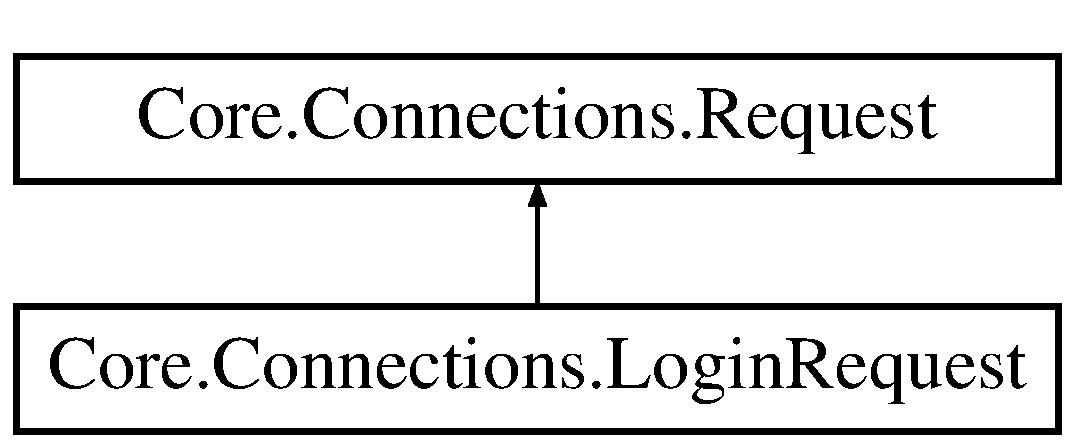
\includegraphics[height=2.000000cm]{classCore_1_1Connections_1_1LoginRequest}
\end{center}
\end{figure}
\subsection*{Public Member Functions}
\begin{DoxyCompactItemize}
\item 
\hyperlink{classCore_1_1Connections_1_1LoginRequest_a5358029b8a55dfbcdd7567f1b812d399}{Login\+Request} (\hyperlink{classCore_1_1Models_1_1Position}{Core.\+Models.\+Position} position, string username, string password)
\begin{DoxyCompactList}\small\item\em Initializes a new instance of the \hyperlink{classCore_1_1Connections_1_1LoginRequest}{Core.\+Connections.\+Login\+Request} class. \end{DoxyCompactList}\end{DoxyCompactItemize}
\subsection*{Public Attributes}
\begin{DoxyCompactItemize}
\item 
string \hyperlink{classCore_1_1Connections_1_1LoginRequest_aead391392278a11f91e5570e44942f91}{Username}
\begin{DoxyCompactList}\small\item\em The Name of the user. \end{DoxyCompactList}\item 
string \hyperlink{classCore_1_1Connections_1_1LoginRequest_af3a2a4f734dcca3404687bfb8844b2ee}{Password}
\begin{DoxyCompactList}\small\item\em The password of the user. \end{DoxyCompactList}\end{DoxyCompactItemize}


\subsection{Detailed Description}
\hyperlink{classCore_1_1Connections_1_1Request}{Request} class which should be used to send actions to the server. Should be serialized before sending, will be deserialized after receiving. 



\subsection{Constructor \& Destructor Documentation}
\hypertarget{classCore_1_1Connections_1_1LoginRequest_a5358029b8a55dfbcdd7567f1b812d399}{}\index{Core\+::\+Connections\+::\+Login\+Request@{Core\+::\+Connections\+::\+Login\+Request}!Login\+Request@{Login\+Request}}
\index{Login\+Request@{Login\+Request}!Core\+::\+Connections\+::\+Login\+Request@{Core\+::\+Connections\+::\+Login\+Request}}
\subsubsection[{Login\+Request(\+Core.\+Models.\+Position position, string username, string password)}]{\setlength{\rightskip}{0pt plus 5cm}Core.\+Connections.\+Login\+Request.\+Login\+Request (
\begin{DoxyParamCaption}
\item[{{\bf Core.\+Models.\+Position}}]{position, }
\item[{string}]{username, }
\item[{string}]{password}
\end{DoxyParamCaption}
)}\label{classCore_1_1Connections_1_1LoginRequest_a5358029b8a55dfbcdd7567f1b812d399}


Initializes a new instance of the \hyperlink{classCore_1_1Connections_1_1LoginRequest}{Core.\+Connections.\+Login\+Request} class. 


\begin{DoxyParams}{Parameters}
{\em position} & Position where the user is standing (converted G\+P\+S information).\\
\hline
{\em username} & User Name.\\
\hline
{\em password} & Password of the user.\\
\hline
\end{DoxyParams}


\subsection{Member Data Documentation}
\hypertarget{classCore_1_1Connections_1_1LoginRequest_af3a2a4f734dcca3404687bfb8844b2ee}{}\index{Core\+::\+Connections\+::\+Login\+Request@{Core\+::\+Connections\+::\+Login\+Request}!Password@{Password}}
\index{Password@{Password}!Core\+::\+Connections\+::\+Login\+Request@{Core\+::\+Connections\+::\+Login\+Request}}
\subsubsection[{Password}]{\setlength{\rightskip}{0pt plus 5cm}string Core.\+Connections.\+Login\+Request.\+Password}\label{classCore_1_1Connections_1_1LoginRequest_af3a2a4f734dcca3404687bfb8844b2ee}


The password of the user. 

\hypertarget{classCore_1_1Connections_1_1LoginRequest_aead391392278a11f91e5570e44942f91}{}\index{Core\+::\+Connections\+::\+Login\+Request@{Core\+::\+Connections\+::\+Login\+Request}!Username@{Username}}
\index{Username@{Username}!Core\+::\+Connections\+::\+Login\+Request@{Core\+::\+Connections\+::\+Login\+Request}}
\subsubsection[{Username}]{\setlength{\rightskip}{0pt plus 5cm}string Core.\+Connections.\+Login\+Request.\+Username}\label{classCore_1_1Connections_1_1LoginRequest_aead391392278a11f91e5570e44942f91}


The Name of the user. 



The documentation for this class was generated from the following file\+:\begin{DoxyCompactItemize}
\item 
base/\+Connection/Login\+Request.\+cs\end{DoxyCompactItemize}

\hypertarget{classCore_1_1Connections_1_1LoginResponse}{\section{Core.\-Connections.\-Login\-Response Class Reference}
\label{classCore_1_1Connections_1_1LoginResponse}\index{Core.\-Connections.\-Login\-Response@{Core.\-Connections.\-Login\-Response}}
}


\hyperlink{classCore_1_1Connections_1_1Response}{Response} class which should be used to login. Will be serialised before sending, should be deserialised after recieving.  


\subsection*{Public Types}
\begin{DoxyCompactItemize}
\item 
enum {\bfseries Reponse\-Status} \{ {\bfseries O\-K}, 
{\bfseries E\-R\-R\-O\-R}
 \}
\end{DoxyCompactItemize}
\subsection*{Public Attributes}
\begin{DoxyCompactItemize}
\item 
\hypertarget{classCore_1_1Connections_1_1LoginResponse_a07d5c565863a18dc114700d9420b2d5f}{Reponse\-Status {\bfseries Status}}\label{classCore_1_1Connections_1_1LoginResponse_a07d5c565863a18dc114700d9420b2d5f}

\item 
\hypertarget{classCore_1_1Connections_1_1LoginResponse_a0852c12c3db05b5f4093ee08f5aa4107}{Guid {\bfseries Session\-I\-D}}\label{classCore_1_1Connections_1_1LoginResponse_a0852c12c3db05b5f4093ee08f5aa4107}

\item 
\hypertarget{classCore_1_1Connections_1_1LoginResponse_a2ef450c94ba6160627b8045a1829c1ff}{int {\bfseries Account\-Id}}\label{classCore_1_1Connections_1_1LoginResponse_a2ef450c94ba6160627b8045a1829c1ff}

\end{DoxyCompactItemize}


\subsection{Detailed Description}
\hyperlink{classCore_1_1Connections_1_1Response}{Response} class which should be used to login. Will be serialised before sending, should be deserialised after recieving. 



The documentation for this class was generated from the following file\-:\begin{DoxyCompactItemize}
\item 
base/\-Connection/Login\-Response.\-cs\end{DoxyCompactItemize}

\hypertarget{classClient_1_1Common_1_1Views_1_1LogoLayer}{\section{Client.\-Common.\-Views.\-Logo\-Layer Class Reference}
\label{classClient_1_1Common_1_1Views_1_1LogoLayer}\index{Client.\-Common.\-Views.\-Logo\-Layer@{Client.\-Common.\-Views.\-Logo\-Layer}}
}
Inheritance diagram for Client.\-Common.\-Views.\-Logo\-Layer\-:\begin{figure}[H]
\begin{center}
\leavevmode
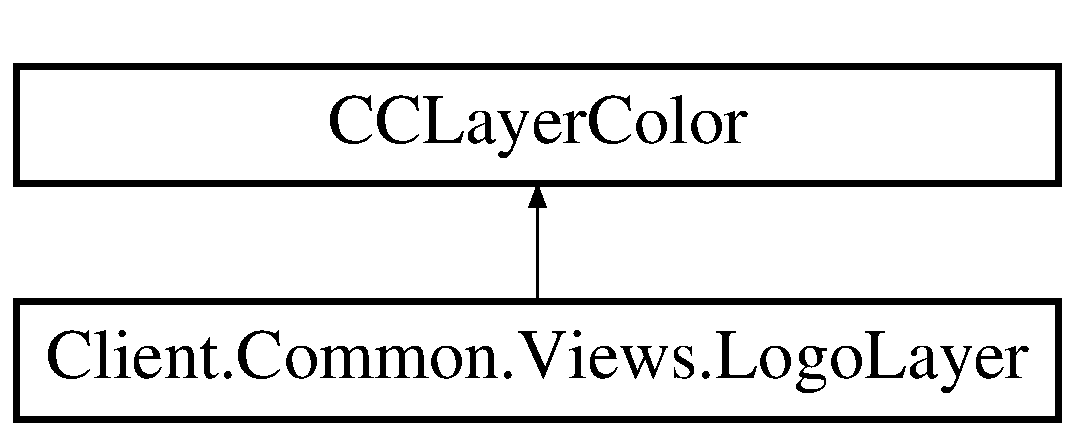
\includegraphics[height=2.000000cm]{classClient_1_1Common_1_1Views_1_1LogoLayer}
\end{center}
\end{figure}
\subsection*{Public Member Functions}
\begin{DoxyCompactItemize}
\item 
\hypertarget{classClient_1_1Common_1_1Views_1_1LogoLayer_a0a0c2ad0ea01f8f6fd135c5259b54d89}{{\bfseries Logo\-Layer} (\hyperlink{classClient_1_1Common_1_1Views_1_1StartScene}{Start\-Scene} start\-Scene)}\label{classClient_1_1Common_1_1Views_1_1LogoLayer_a0a0c2ad0ea01f8f6fd135c5259b54d89}

\end{DoxyCompactItemize}
\subsection*{Protected Member Functions}
\begin{DoxyCompactItemize}
\item 
\hypertarget{classClient_1_1Common_1_1Views_1_1LogoLayer_ab7adc83ae509b73ddeb815f96fe26f10}{override void {\bfseries Added\-To\-Scene} ()}\label{classClient_1_1Common_1_1Views_1_1LogoLayer_ab7adc83ae509b73ddeb815f96fe26f10}

\end{DoxyCompactItemize}


The documentation for this class was generated from the following file\-:\begin{DoxyCompactItemize}
\item 
client/client/client.\-Common/\-Views/Logo\-Layer.\-cs\end{DoxyCompactItemize}

\hypertarget{classClient_1_1Droid_1_1MainActivity}{\section{Client.\-Droid.\-Main\-Activity Class Reference}
\label{classClient_1_1Droid_1_1MainActivity}\index{Client.\-Droid.\-Main\-Activity@{Client.\-Droid.\-Main\-Activity}}
}
Inheritance diagram for Client.\-Droid.\-Main\-Activity\-:\begin{figure}[H]
\begin{center}
\leavevmode
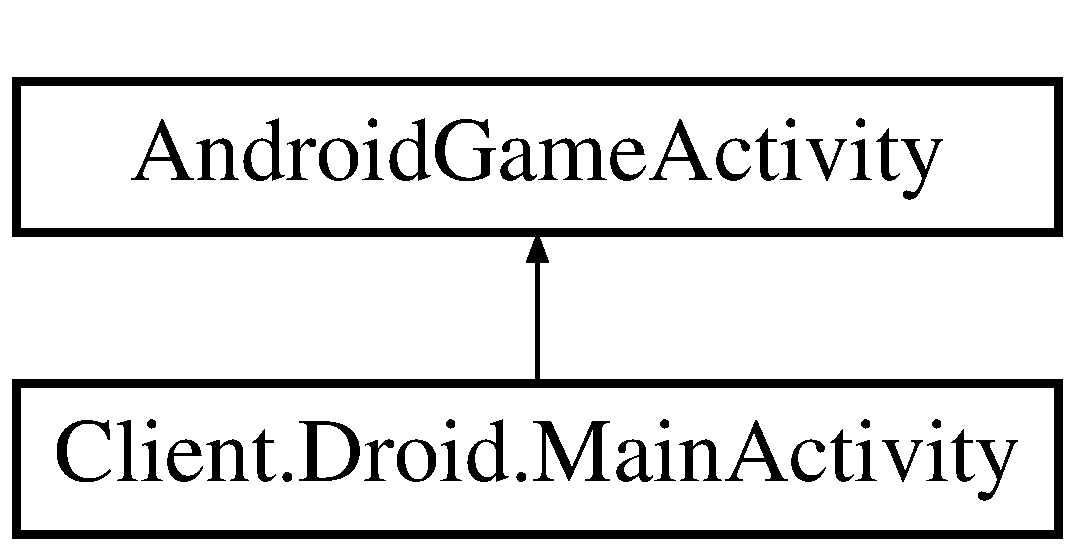
\includegraphics[height=2.000000cm]{classClient_1_1Droid_1_1MainActivity}
\end{center}
\end{figure}
\subsection*{Protected Member Functions}
\begin{DoxyCompactItemize}
\item 
\hypertarget{classClient_1_1Droid_1_1MainActivity_a81c1652b05e56f45d7d6291f2fee2e3a}{override void {\bfseries On\-Create} (Bundle bundle)}\label{classClient_1_1Droid_1_1MainActivity_a81c1652b05e56f45d7d6291f2fee2e3a}

\end{DoxyCompactItemize}


The documentation for this class was generated from the following file\-:\begin{DoxyCompactItemize}
\item 
client/client/client.\-Android/Main\-Activity.\-cs\end{DoxyCompactItemize}

\hypertarget{classtest_1_1MainClass}{}\section{test.\+Main\+Class Class Reference}
\label{classtest_1_1MainClass}\index{test.\+Main\+Class@{test.\+Main\+Class}}
\subsection*{Static Public Member Functions}
\begin{DoxyCompactItemize}
\item 
\hypertarget{classtest_1_1MainClass_a4679ef28a1326b8af55f556b1b0e94a7}{}static void {\bfseries Main} (string\mbox{[}$\,$\mbox{]} args)\label{classtest_1_1MainClass_a4679ef28a1326b8af55f556b1b0e94a7}

\end{DoxyCompactItemize}


The documentation for this class was generated from the following file\+:\begin{DoxyCompactItemize}
\item 
test/Program.\+cs\end{DoxyCompactItemize}

\hypertarget{classClient_1_1Common_1_1Models_1_1MapCellPosition}{\section{Client.\-Common.\-Models.\-Map\-Cell\-Position Class Reference}
\label{classClient_1_1Common_1_1Models_1_1MapCellPosition}\index{Client.\-Common.\-Models.\-Map\-Cell\-Position@{Client.\-Common.\-Models.\-Map\-Cell\-Position}}
}
\subsection*{Public Member Functions}
\begin{DoxyCompactItemize}
\item 
\hypertarget{classClient_1_1Common_1_1Models_1_1MapCellPosition_a0a1cdb4e682db8251922ad0628f9b39d}{{\bfseries Map\-Cell\-Position} (int cell\-X, int cell\-Y)}\label{classClient_1_1Common_1_1Models_1_1MapCellPosition_a0a1cdb4e682db8251922ad0628f9b39d}

\item 
\hypertarget{classClient_1_1Common_1_1Models_1_1MapCellPosition_a64af2cde673de32a8bddde96589f2e77}{{\bfseries Map\-Cell\-Position} (C\-C\-Tile\-Map\-Coordinates tile\-Map\-Coordinates)}\label{classClient_1_1Common_1_1Models_1_1MapCellPosition_a64af2cde673de32a8bddde96589f2e77}

\item 
\hypertarget{classClient_1_1Common_1_1Models_1_1MapCellPosition_a01720d038f8cbaa8e2a3aa003fc434a4}{C\-C\-Tile\-Map\-Coordinates {\bfseries Get\-Tile\-Map\-Coordinates} ()}\label{classClient_1_1Common_1_1Models_1_1MapCellPosition_a01720d038f8cbaa8e2a3aa003fc434a4}

\item 
\hypertarget{classClient_1_1Common_1_1Models_1_1MapCellPosition_a401686dcad08fee1b8884f562d12a630}{C\-C\-Point {\bfseries Get\-Anchor} ()}\label{classClient_1_1Common_1_1Models_1_1MapCellPosition_a401686dcad08fee1b8884f562d12a630}

\end{DoxyCompactItemize}
\subsection*{Properties}
\begin{DoxyCompactItemize}
\item 
\hypertarget{classClient_1_1Common_1_1Models_1_1MapCellPosition_a3698c44e12f74fef06625e4bf751620c}{int {\bfseries Cell\-X}\hspace{0.3cm}{\ttfamily  \mbox{[}get\mbox{]}}}\label{classClient_1_1Common_1_1Models_1_1MapCellPosition_a3698c44e12f74fef06625e4bf751620c}

\item 
\hypertarget{classClient_1_1Common_1_1Models_1_1MapCellPosition_a4051441b879311d5f933fa6a801ed2cd}{int {\bfseries Cell\-Y}\hspace{0.3cm}{\ttfamily  \mbox{[}get\mbox{]}}}\label{classClient_1_1Common_1_1Models_1_1MapCellPosition_a4051441b879311d5f933fa6a801ed2cd}

\end{DoxyCompactItemize}


The documentation for this class was generated from the following file\-:\begin{DoxyCompactItemize}
\item 
client/client/client.\-Common/\-Models/Map\-Cell\-Position.\-cs\end{DoxyCompactItemize}

\hypertarget{classSQLite_1_1MaxLengthAttribute}{\section{S\-Q\-Lite.\-Max\-Length\-Attribute Class Reference}
\label{classSQLite_1_1MaxLengthAttribute}\index{S\-Q\-Lite.\-Max\-Length\-Attribute@{S\-Q\-Lite.\-Max\-Length\-Attribute}}
}
Inheritance diagram for S\-Q\-Lite.\-Max\-Length\-Attribute\-:\begin{figure}[H]
\begin{center}
\leavevmode
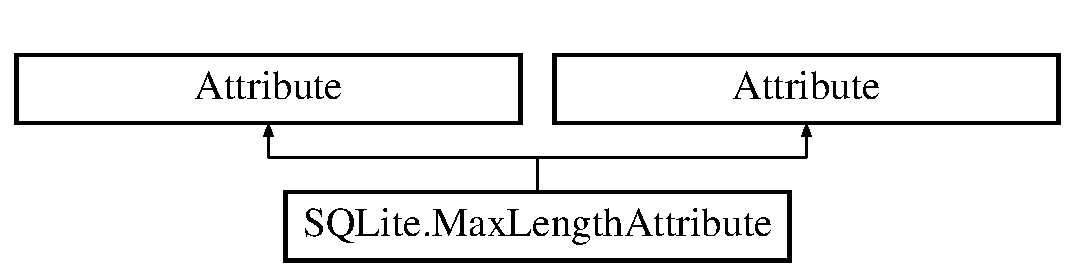
\includegraphics[height=2.000000cm]{classSQLite_1_1MaxLengthAttribute}
\end{center}
\end{figure}
\subsection*{Public Member Functions}
\begin{DoxyCompactItemize}
\item 
\hypertarget{classSQLite_1_1MaxLengthAttribute_ade550746d23ce2d766d0e1debe57c606}{{\bfseries Max\-Length\-Attribute} (int length)}\label{classSQLite_1_1MaxLengthAttribute_ade550746d23ce2d766d0e1debe57c606}

\item 
\hypertarget{classSQLite_1_1MaxLengthAttribute_ade550746d23ce2d766d0e1debe57c606}{{\bfseries Max\-Length\-Attribute} (int length)}\label{classSQLite_1_1MaxLengthAttribute_ade550746d23ce2d766d0e1debe57c606}

\end{DoxyCompactItemize}
\subsection*{Properties}
\begin{DoxyCompactItemize}
\item 
\hypertarget{classSQLite_1_1MaxLengthAttribute_a12e006bbd11ded434ccba4873d48b84a}{int {\bfseries Value}\hspace{0.3cm}{\ttfamily  \mbox{[}get, set\mbox{]}}}\label{classSQLite_1_1MaxLengthAttribute_a12e006bbd11ded434ccba4873d48b84a}

\end{DoxyCompactItemize}


The documentation for this class was generated from the following file\-:\begin{DoxyCompactItemize}
\item 
packages/sqlite-\/net.\-1.\-0.\-8/content/S\-Q\-Lite.\-cs\end{DoxyCompactItemize}

\hypertarget{classClient_1_1Common_1_1Views_1_1MenuView}{\section{Client.\-Common.\-Views.\-Menu\-View Class Reference}
\label{classClient_1_1Common_1_1Views_1_1MenuView}\index{Client.\-Common.\-Views.\-Menu\-View@{Client.\-Common.\-Views.\-Menu\-View}}
}
\subsection*{Public Member Functions}
\begin{DoxyCompactItemize}
\item 
\hypertarget{classClient_1_1Common_1_1Views_1_1MenuView_a625e8f113e66ae12b1ebb9142ef9072d}{{\bfseries Menu\-View} (C\-C\-Tile\-Map\-Layer menu\-Layer, C\-C\-Tile\-Map\-Coordinates center, \hyperlink{classCore_1_1Models_1_1Definitions_1_1Definition}{Definition}\mbox{[}$\,$\mbox{]} types)}\label{classClient_1_1Common_1_1Views_1_1MenuView_a625e8f113e66ae12b1ebb9142ef9072d}

\item 
\hypertarget{classClient_1_1Common_1_1Views_1_1MenuView_aab5290ebf833abcf80e67c46199cb53d}{C\-C\-Tile\-Map\-Coordinates\mbox{[}$\,$\mbox{]} {\bfseries Get\-Surrounded\-Tiles} ()}\label{classClient_1_1Common_1_1Views_1_1MenuView_aab5290ebf833abcf80e67c46199cb53d}

\item 
void \hyperlink{classClient_1_1Common_1_1Views_1_1MenuView_a52c67c8cd89babbf271a40f01e627b7a}{Draw\-Menu} ()
\begin{DoxyCompactList}\small\item\em Shows the menu at a given Location. \end{DoxyCompactList}\item 
\hypertarget{classClient_1_1Common_1_1Views_1_1MenuView_ae8d1c45d630862f67843b76195c2c5dd}{\hyperlink{classCore_1_1Models_1_1Definitions_1_1Definition}{Core.\-Models.\-Definitions.\-Definition} {\bfseries Get\-Selected\-Definition} (C\-C\-Tile\-Map\-Coordinates coord)}\label{classClient_1_1Common_1_1Views_1_1MenuView_ae8d1c45d630862f67843b76195c2c5dd}

\item 
void \hyperlink{classClient_1_1Common_1_1Views_1_1MenuView_abd8d48d776f40caf15251786866331bc}{Close\-Menu} ()
\begin{DoxyCompactList}\small\item\em Closes the menu. \end{DoxyCompactList}\end{DoxyCompactItemize}


\subsection{Member Function Documentation}
\hypertarget{classClient_1_1Common_1_1Views_1_1MenuView_abd8d48d776f40caf15251786866331bc}{\index{Client\-::\-Common\-::\-Views\-::\-Menu\-View@{Client\-::\-Common\-::\-Views\-::\-Menu\-View}!Close\-Menu@{Close\-Menu}}
\index{Close\-Menu@{Close\-Menu}!Client::Common::Views::MenuView@{Client\-::\-Common\-::\-Views\-::\-Menu\-View}}
\subsubsection[{Close\-Menu}]{\setlength{\rightskip}{0pt plus 5cm}void Client.\-Common.\-Views.\-Menu\-View.\-Close\-Menu (
\begin{DoxyParamCaption}
{}
\end{DoxyParamCaption}
)\hspace{0.3cm}{\ttfamily [inline]}}}\label{classClient_1_1Common_1_1Views_1_1MenuView_abd8d48d776f40caf15251786866331bc}


Closes the menu. 

\hypertarget{classClient_1_1Common_1_1Views_1_1MenuView_a52c67c8cd89babbf271a40f01e627b7a}{\index{Client\-::\-Common\-::\-Views\-::\-Menu\-View@{Client\-::\-Common\-::\-Views\-::\-Menu\-View}!Draw\-Menu@{Draw\-Menu}}
\index{Draw\-Menu@{Draw\-Menu}!Client::Common::Views::MenuView@{Client\-::\-Common\-::\-Views\-::\-Menu\-View}}
\subsubsection[{Draw\-Menu}]{\setlength{\rightskip}{0pt plus 5cm}void Client.\-Common.\-Views.\-Menu\-View.\-Draw\-Menu (
\begin{DoxyParamCaption}
{}
\end{DoxyParamCaption}
)\hspace{0.3cm}{\ttfamily [inline]}}}\label{classClient_1_1Common_1_1Views_1_1MenuView_a52c67c8cd89babbf271a40f01e627b7a}


Shows the menu at a given Location. 


\begin{DoxyParams}{Parameters}
{\em location} & Touch Location.\\
\hline
{\em menutype} & Menutype.\\
\hline
\end{DoxyParams}


The documentation for this class was generated from the following file\-:\begin{DoxyCompactItemize}
\item 
client/client/client.\-Common/\-Views/Menu\-View.\-cs\end{DoxyCompactItemize}

\hypertarget{classCore_1_1Models_1_1ModelEntity}{\section{Core.\-Models.\-Model\-Entity Class Reference}
\label{classCore_1_1Models_1_1ModelEntity}\index{Core.\-Models.\-Model\-Entity@{Core.\-Models.\-Model\-Entity}}
}


M\-V\-C Model.  


Inheritance diagram for Core.\-Models.\-Model\-Entity\-:\begin{figure}[H]
\begin{center}
\leavevmode
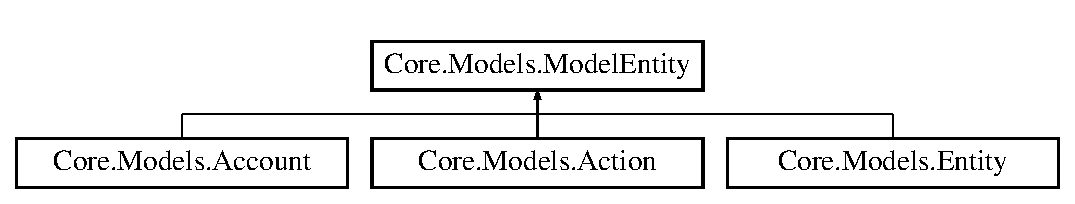
\includegraphics[height=2.000000cm]{classCore_1_1Models_1_1ModelEntity}
\end{center}
\end{figure}
\subsection*{Public Attributes}
\begin{DoxyCompactItemize}
\item 
\hypertarget{classCore_1_1Models_1_1ModelEntity_a19619acbb856f7b54c971b38f061509c}{\hyperlink{classCore_1_1Views_1_1ViewEntity}{Views.\-View\-Entity} {\bfseries View}}\label{classCore_1_1Models_1_1ModelEntity_a19619acbb856f7b54c971b38f061509c}

\item 
\hypertarget{classCore_1_1Models_1_1ModelEntity_a78a6ddcf09a0b517230e738c40faa813}{\hyperlink{classCore_1_1Controllers_1_1ControlEntity}{Controllers.\-Control\-Entity} {\bfseries Control}}\label{classCore_1_1Models_1_1ModelEntity_a78a6ddcf09a0b517230e738c40faa813}

\end{DoxyCompactItemize}


\subsection{Detailed Description}
M\-V\-C Model. 



The documentation for this class was generated from the following file\-:\begin{DoxyCompactItemize}
\item 
base/\-Models/Model\-Entity.\-cs\end{DoxyCompactItemize}

\hypertarget{classCore_1_1Controllers_1_1Actions_1_1MoveUnit}{\section{Core.\-Controllers.\-Actions.\-Move\-Unit Class Reference}
\label{classCore_1_1Controllers_1_1Actions_1_1MoveUnit}\index{Core.\-Controllers.\-Actions.\-Move\-Unit@{Core.\-Controllers.\-Actions.\-Move\-Unit}}
}
Inheritance diagram for Core.\-Controllers.\-Actions.\-Move\-Unit\-:\begin{figure}[H]
\begin{center}
\leavevmode
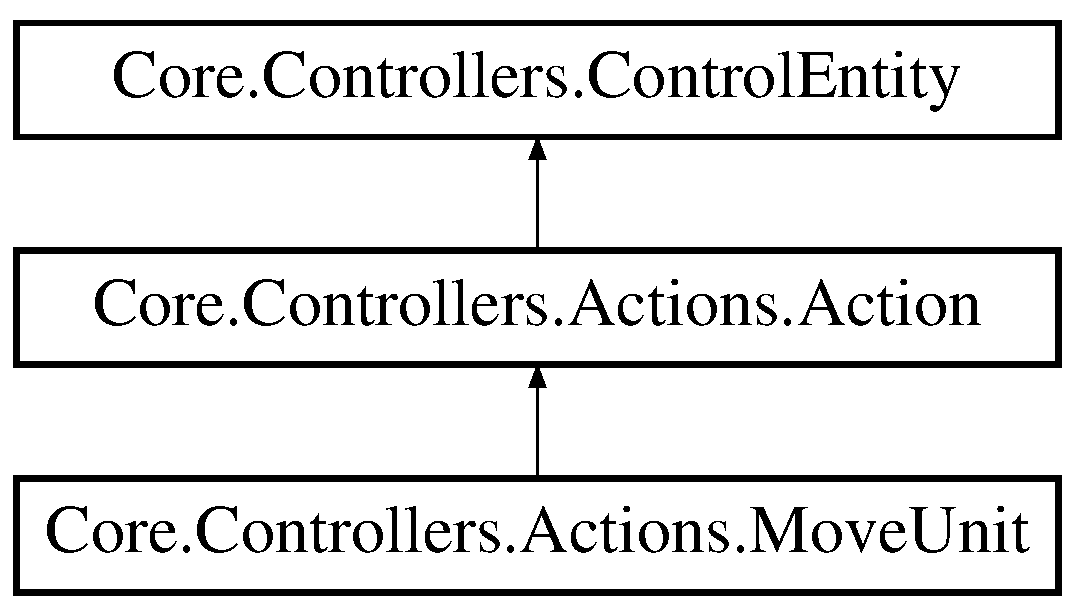
\includegraphics[height=3.000000cm]{classCore_1_1Controllers_1_1Actions_1_1MoveUnit}
\end{center}
\end{figure}
\subsection*{Public Member Functions}
\begin{DoxyCompactItemize}
\item 
\hyperlink{classCore_1_1Controllers_1_1Actions_1_1MoveUnit_a323064ada90151bcd8d659ee27d87917}{Move\-Unit} (\hyperlink{classCore_1_1Models_1_1ModelEntity}{Core.\-Models.\-Model\-Entity} model)
\begin{DoxyCompactList}\small\item\em Initializes a new instance of the Core.\-Models.\-Actions.\-Move\-Unit class. \end{DoxyCompactList}\item 
override Concurrent\-Bag\\*
$<$ \hyperlink{classCore_1_1Models_1_1Region}{Core.\-Models.\-Region} $>$ \hyperlink{classCore_1_1Controllers_1_1Actions_1_1MoveUnit_a0331c4888d9efc148ecc501b4db37481}{Get\-Affected\-Regions} ()
\begin{DoxyCompactList}\small\item\em Gets the affected regions. \end{DoxyCompactList}\item 
override bool \hyperlink{classCore_1_1Controllers_1_1Actions_1_1MoveUnit_a6689af13f9a2f8ff90ad72d2ac327a52}{Possible} ()
\begin{DoxyCompactList}\small\item\em Returns true if the action is even possible. \end{DoxyCompactList}\item 
override Concurrent\-Bag\\*
$<$ \hyperlink{classCore_1_1Models_1_1Region}{Core.\-Models.\-Region} $>$ \hyperlink{classCore_1_1Controllers_1_1Actions_1_1MoveUnit_adaf6b91a2e858d8805ea8ed83947b27a}{Do} ()
\begin{DoxyCompactList}\small\item\em Apply action-\/related changes to the world. Returns set of changed Regions if everything worked, otherwise null \end{DoxyCompactList}\item 
override bool \hyperlink{classCore_1_1Controllers_1_1Actions_1_1MoveUnit_a80ff3497561ed98a933e41f48830d947}{Catch} ()
\begin{DoxyCompactList}\small\item\em In case of errors, revert the world data to a valid state. \end{DoxyCompactList}\item 
override \hyperlink{classCore_1_1Models_1_1RegionPosition}{Core.\-Models.\-Region\-Position} \hyperlink{classCore_1_1Controllers_1_1Actions_1_1MoveUnit_a87a9c5589011c8e86770e1b1be487381}{Get\-Region\-Position} ()
\begin{DoxyCompactList}\small\item\em Gets the region position. \end{DoxyCompactList}\end{DoxyCompactItemize}
\subsection*{Public Attributes}
\begin{DoxyCompactItemize}
\item 
\hypertarget{classCore_1_1Controllers_1_1Actions_1_1MoveUnit_aa00af18610776c1a0eebde8ae273286a}{const string {\bfseries S\-T\-A\-R\-T\-\_\-\-P\-O\-S\-I\-T\-I\-O\-N} = \char`\"{}Entity\-Position\char`\"{}}\label{classCore_1_1Controllers_1_1Actions_1_1MoveUnit_aa00af18610776c1a0eebde8ae273286a}

\item 
\hypertarget{classCore_1_1Controllers_1_1Actions_1_1MoveUnit_a411193c1cf0e0784fbc3340dcc3cd21c}{const string {\bfseries E\-N\-D\-\_\-\-P\-O\-S\-I\-T\-I\-O\-N} = \char`\"{}New\-Position\char`\"{}}\label{classCore_1_1Controllers_1_1Actions_1_1MoveUnit_a411193c1cf0e0784fbc3340dcc3cd21c}

\item 
\hypertarget{classCore_1_1Controllers_1_1Actions_1_1MoveUnit_a32d0ea3d4b02301de1b754a4e8bcaacd}{I\-List {\bfseries Path}}\label{classCore_1_1Controllers_1_1Actions_1_1MoveUnit_a32d0ea3d4b02301de1b754a4e8bcaacd}

\end{DoxyCompactItemize}
\subsection*{Additional Inherited Members}


\subsection{Constructor \& Destructor Documentation}
\hypertarget{classCore_1_1Controllers_1_1Actions_1_1MoveUnit_a323064ada90151bcd8d659ee27d87917}{\index{Core\-::\-Controllers\-::\-Actions\-::\-Move\-Unit@{Core\-::\-Controllers\-::\-Actions\-::\-Move\-Unit}!Move\-Unit@{Move\-Unit}}
\index{Move\-Unit@{Move\-Unit}!Core::Controllers::Actions::MoveUnit@{Core\-::\-Controllers\-::\-Actions\-::\-Move\-Unit}}
\subsubsection[{Move\-Unit}]{\setlength{\rightskip}{0pt plus 5cm}Core.\-Controllers.\-Actions.\-Move\-Unit.\-Move\-Unit (
\begin{DoxyParamCaption}
\item[{{\bf Core.\-Models.\-Model\-Entity}}]{model}
\end{DoxyParamCaption}
)\hspace{0.3cm}{\ttfamily [inline]}}}\label{classCore_1_1Controllers_1_1Actions_1_1MoveUnit_a323064ada90151bcd8d659ee27d87917}


Initializes a new instance of the Core.\-Models.\-Actions.\-Move\-Unit class. 


\begin{DoxyParams}{Parameters}
{\em model} & Model.\\
\hline
\end{DoxyParams}


\subsection{Member Function Documentation}
\hypertarget{classCore_1_1Controllers_1_1Actions_1_1MoveUnit_a80ff3497561ed98a933e41f48830d947}{\index{Core\-::\-Controllers\-::\-Actions\-::\-Move\-Unit@{Core\-::\-Controllers\-::\-Actions\-::\-Move\-Unit}!Catch@{Catch}}
\index{Catch@{Catch}!Core::Controllers::Actions::MoveUnit@{Core\-::\-Controllers\-::\-Actions\-::\-Move\-Unit}}
\subsubsection[{Catch}]{\setlength{\rightskip}{0pt plus 5cm}override bool Core.\-Controllers.\-Actions.\-Move\-Unit.\-Catch (
\begin{DoxyParamCaption}
{}
\end{DoxyParamCaption}
)\hspace{0.3cm}{\ttfamily [inline]}, {\ttfamily [virtual]}}}\label{classCore_1_1Controllers_1_1Actions_1_1MoveUnit_a80ff3497561ed98a933e41f48830d947}


In case of errors, revert the world data to a valid state. 



Reimplemented from \hyperlink{classCore_1_1Controllers_1_1Actions_1_1Action_ada4c77dfeee78ded10a6eb6a506defb4}{Core.\-Controllers.\-Actions.\-Action}.

\hypertarget{classCore_1_1Controllers_1_1Actions_1_1MoveUnit_adaf6b91a2e858d8805ea8ed83947b27a}{\index{Core\-::\-Controllers\-::\-Actions\-::\-Move\-Unit@{Core\-::\-Controllers\-::\-Actions\-::\-Move\-Unit}!Do@{Do}}
\index{Do@{Do}!Core::Controllers::Actions::MoveUnit@{Core\-::\-Controllers\-::\-Actions\-::\-Move\-Unit}}
\subsubsection[{Do}]{\setlength{\rightskip}{0pt plus 5cm}override Concurrent\-Bag$<${\bf Core.\-Models.\-Region}$>$ Core.\-Controllers.\-Actions.\-Move\-Unit.\-Do (
\begin{DoxyParamCaption}
{}
\end{DoxyParamCaption}
)\hspace{0.3cm}{\ttfamily [inline]}, {\ttfamily [virtual]}}}\label{classCore_1_1Controllers_1_1Actions_1_1MoveUnit_adaf6b91a2e858d8805ea8ed83947b27a}


Apply action-\/related changes to the world. Returns set of changed Regions if everything worked, otherwise null 


\begin{DoxyParams}{Parameters}
{\em region\-Manager\-C} & Region manager c.\\
\hline
\end{DoxyParams}


Reimplemented from \hyperlink{classCore_1_1Controllers_1_1Actions_1_1Action_afbb091ee28eee896951fac600188d446}{Core.\-Controllers.\-Actions.\-Action}.

\hypertarget{classCore_1_1Controllers_1_1Actions_1_1MoveUnit_a0331c4888d9efc148ecc501b4db37481}{\index{Core\-::\-Controllers\-::\-Actions\-::\-Move\-Unit@{Core\-::\-Controllers\-::\-Actions\-::\-Move\-Unit}!Get\-Affected\-Regions@{Get\-Affected\-Regions}}
\index{Get\-Affected\-Regions@{Get\-Affected\-Regions}!Core::Controllers::Actions::MoveUnit@{Core\-::\-Controllers\-::\-Actions\-::\-Move\-Unit}}
\subsubsection[{Get\-Affected\-Regions}]{\setlength{\rightskip}{0pt plus 5cm}override Concurrent\-Bag$<${\bf Core.\-Models.\-Region}$>$ Core.\-Controllers.\-Actions.\-Move\-Unit.\-Get\-Affected\-Regions (
\begin{DoxyParamCaption}
{}
\end{DoxyParamCaption}
)\hspace{0.3cm}{\ttfamily [inline]}, {\ttfamily [virtual]}}}\label{classCore_1_1Controllers_1_1Actions_1_1MoveUnit_a0331c4888d9efc148ecc501b4db37481}


Gets the affected regions. 

\begin{DoxyReturn}{Returns}
The affected regions.
\end{DoxyReturn}

\begin{DoxyParams}{Parameters}
{\em region\-Manager\-C} & Region manager c.\\
\hline
\end{DoxyParams}


Reimplemented from \hyperlink{classCore_1_1Controllers_1_1Actions_1_1Action_aa11bdeffff43ec47ac7c3d6843a85674}{Core.\-Controllers.\-Actions.\-Action}.

\hypertarget{classCore_1_1Controllers_1_1Actions_1_1MoveUnit_a87a9c5589011c8e86770e1b1be487381}{\index{Core\-::\-Controllers\-::\-Actions\-::\-Move\-Unit@{Core\-::\-Controllers\-::\-Actions\-::\-Move\-Unit}!Get\-Region\-Position@{Get\-Region\-Position}}
\index{Get\-Region\-Position@{Get\-Region\-Position}!Core::Controllers::Actions::MoveUnit@{Core\-::\-Controllers\-::\-Actions\-::\-Move\-Unit}}
\subsubsection[{Get\-Region\-Position}]{\setlength{\rightskip}{0pt plus 5cm}override {\bf Core.\-Models.\-Region\-Position} Core.\-Controllers.\-Actions.\-Move\-Unit.\-Get\-Region\-Position (
\begin{DoxyParamCaption}
{}
\end{DoxyParamCaption}
)\hspace{0.3cm}{\ttfamily [inline]}, {\ttfamily [virtual]}}}\label{classCore_1_1Controllers_1_1Actions_1_1MoveUnit_a87a9c5589011c8e86770e1b1be487381}


Gets the region position. 

\begin{DoxyReturn}{Returns}
The region position.
\end{DoxyReturn}


Reimplemented from \hyperlink{classCore_1_1Controllers_1_1Actions_1_1Action_a6ffe3c30cb5648a81f50096f4f332d5a}{Core.\-Controllers.\-Actions.\-Action}.

\hypertarget{classCore_1_1Controllers_1_1Actions_1_1MoveUnit_a6689af13f9a2f8ff90ad72d2ac327a52}{\index{Core\-::\-Controllers\-::\-Actions\-::\-Move\-Unit@{Core\-::\-Controllers\-::\-Actions\-::\-Move\-Unit}!Possible@{Possible}}
\index{Possible@{Possible}!Core::Controllers::Actions::MoveUnit@{Core\-::\-Controllers\-::\-Actions\-::\-Move\-Unit}}
\subsubsection[{Possible}]{\setlength{\rightskip}{0pt plus 5cm}override bool Core.\-Controllers.\-Actions.\-Move\-Unit.\-Possible (
\begin{DoxyParamCaption}
{}
\end{DoxyParamCaption}
)\hspace{0.3cm}{\ttfamily [inline]}, {\ttfamily [virtual]}}}\label{classCore_1_1Controllers_1_1Actions_1_1MoveUnit_a6689af13f9a2f8ff90ad72d2ac327a52}


Returns true if the action is even possible. 


\begin{DoxyParams}{Parameters}
{\em region\-Manager\-C} & Region manager c.\\
\hline
\end{DoxyParams}


Reimplemented from \hyperlink{classCore_1_1Controllers_1_1Actions_1_1Action_a405b995343a9394ad19e05a699a4e6d9}{Core.\-Controllers.\-Actions.\-Action}.



The documentation for this class was generated from the following file\-:\begin{DoxyCompactItemize}
\item 
base/\-Controllers/\-Action/Move\-Unit.\-cs\end{DoxyCompactItemize}

\hypertarget{classClient_1_1Common_1_1Views_1_1Actions_1_1MoveUnit}{\section{Client.\-Common.\-Views.\-Actions.\-Move\-Unit Class Reference}
\label{classClient_1_1Common_1_1Views_1_1Actions_1_1MoveUnit}\index{Client.\-Common.\-Views.\-Actions.\-Move\-Unit@{Client.\-Common.\-Views.\-Actions.\-Move\-Unit}}
}
Inheritance diagram for Client.\-Common.\-Views.\-Actions.\-Move\-Unit\-:\begin{figure}[H]
\begin{center}
\leavevmode
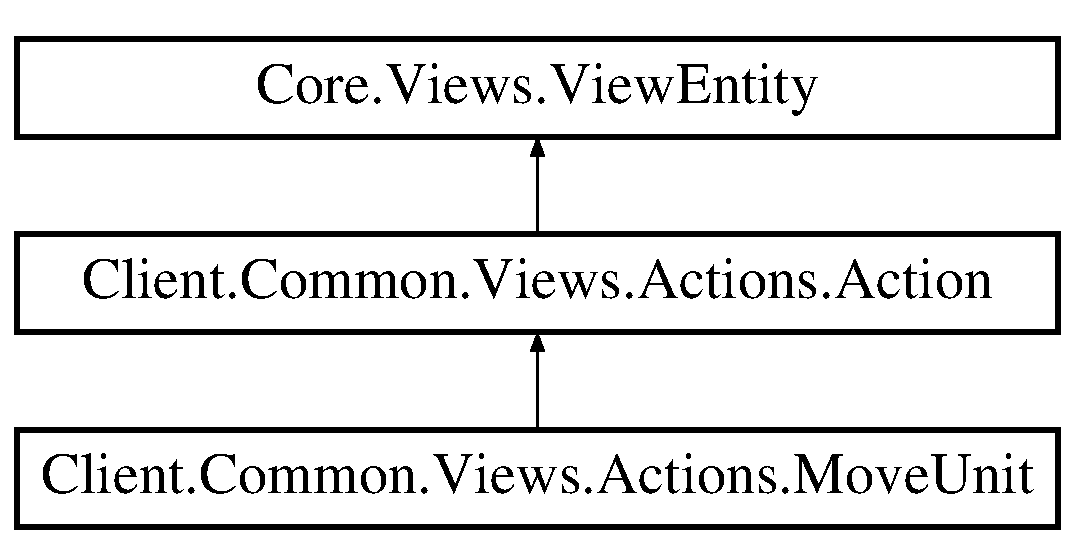
\includegraphics[height=3.000000cm]{classClient_1_1Common_1_1Views_1_1Actions_1_1MoveUnit}
\end{center}
\end{figure}
\subsection*{Public Member Functions}
\begin{DoxyCompactItemize}
\item 
\hypertarget{classClient_1_1Common_1_1Views_1_1Actions_1_1MoveUnit_a319fe131766962c21c60417a582880bd}{{\bfseries Move\-Unit} (\hyperlink{classCore_1_1Models_1_1ModelEntity}{Core.\-Models.\-Model\-Entity} model, \hyperlink{classClient_1_1Common_1_1Views_1_1WorldLayer}{World\-Layer} world\-Layer)}\label{classClient_1_1Common_1_1Views_1_1Actions_1_1MoveUnit_a319fe131766962c21c60417a582880bd}

\item 
override void \hyperlink{classClient_1_1Common_1_1Views_1_1Actions_1_1MoveUnit_a781a55c5c7523ceeee2f64e275d35d09}{Before\-Do} ()
\begin{DoxyCompactList}\small\item\em Gets called before Action\-Control.\-Do() gets executed. Should get and store data which will be needed in Schedule. \end{DoxyCompactList}\item 
override bool \hyperlink{classClient_1_1Common_1_1Views_1_1Actions_1_1MoveUnit_a320dbf0d26ea3e24cfe87eedb61a2e22}{Schedule} (float frame\-Times\-In\-Second)
\begin{DoxyCompactList}\small\item\em Schedules the action. Should do anything do animate the action (e.\-g. draw the entity, animate his moving or start/end animating a fight) Returns true if the action has ended, otherwise false. \end{DoxyCompactList}\end{DoxyCompactItemize}
\subsection*{Properties}
\begin{DoxyCompactItemize}
\item 
\hypertarget{classClient_1_1Common_1_1Views_1_1Actions_1_1MoveUnit_a379b470facc4ffa1df7e9132292a19e1}{\hyperlink{classClient_1_1Common_1_1Views_1_1WorldLayer}{World\-Layer} {\bfseries World\-Layer}\hspace{0.3cm}{\ttfamily  \mbox{[}get, set\mbox{]}}}\label{classClient_1_1Common_1_1Views_1_1Actions_1_1MoveUnit_a379b470facc4ffa1df7e9132292a19e1}

\end{DoxyCompactItemize}


\subsection{Member Function Documentation}
\hypertarget{classClient_1_1Common_1_1Views_1_1Actions_1_1MoveUnit_a781a55c5c7523ceeee2f64e275d35d09}{\index{Client\-::\-Common\-::\-Views\-::\-Actions\-::\-Move\-Unit@{Client\-::\-Common\-::\-Views\-::\-Actions\-::\-Move\-Unit}!Before\-Do@{Before\-Do}}
\index{Before\-Do@{Before\-Do}!Client::Common::Views::Actions::MoveUnit@{Client\-::\-Common\-::\-Views\-::\-Actions\-::\-Move\-Unit}}
\subsubsection[{Before\-Do}]{\setlength{\rightskip}{0pt plus 5cm}override void Client.\-Common.\-Views.\-Actions.\-Move\-Unit.\-Before\-Do (
\begin{DoxyParamCaption}
{}
\end{DoxyParamCaption}
)\hspace{0.3cm}{\ttfamily [inline]}, {\ttfamily [virtual]}}}\label{classClient_1_1Common_1_1Views_1_1Actions_1_1MoveUnit_a781a55c5c7523ceeee2f64e275d35d09}


Gets called before Action\-Control.\-Do() gets executed. Should get and store data which will be needed in Schedule. 



Reimplemented from \hyperlink{classClient_1_1Common_1_1Views_1_1Actions_1_1Action_ad129f8cb1d8079f76d8199dbc80d3c0d}{Client.\-Common.\-Views.\-Actions.\-Action}.

\hypertarget{classClient_1_1Common_1_1Views_1_1Actions_1_1MoveUnit_a320dbf0d26ea3e24cfe87eedb61a2e22}{\index{Client\-::\-Common\-::\-Views\-::\-Actions\-::\-Move\-Unit@{Client\-::\-Common\-::\-Views\-::\-Actions\-::\-Move\-Unit}!Schedule@{Schedule}}
\index{Schedule@{Schedule}!Client::Common::Views::Actions::MoveUnit@{Client\-::\-Common\-::\-Views\-::\-Actions\-::\-Move\-Unit}}
\subsubsection[{Schedule}]{\setlength{\rightskip}{0pt plus 5cm}override bool Client.\-Common.\-Views.\-Actions.\-Move\-Unit.\-Schedule (
\begin{DoxyParamCaption}
\item[{float}]{frame\-Times\-In\-Second}
\end{DoxyParamCaption}
)\hspace{0.3cm}{\ttfamily [inline]}, {\ttfamily [virtual]}}}\label{classClient_1_1Common_1_1Views_1_1Actions_1_1MoveUnit_a320dbf0d26ea3e24cfe87eedb61a2e22}


Schedules the action. Should do anything do animate the action (e.\-g. draw the entity, animate his moving or start/end animating a fight) Returns true if the action has ended, otherwise false. 


\begin{DoxyParams}{Parameters}
{\em frame\-Times\-In\-Second} & frames times in seconds.\\
\hline
\end{DoxyParams}


Reimplemented from \hyperlink{classClient_1_1Common_1_1Views_1_1Actions_1_1Action_a92fdf89fb39016ef84e08dc3c7352d51}{Client.\-Common.\-Views.\-Actions.\-Action}.



The documentation for this class was generated from the following file\-:\begin{DoxyCompactItemize}
\item 
client/client/client.\-Common/\-Views/\-Actions/Move\-Unit.\-cs\end{DoxyCompactItemize}

\hypertarget{classServer_1_1MvcApplication}{\section{Server.\-Mvc\-Application Class Reference}
\label{classServer_1_1MvcApplication}\index{Server.\-Mvc\-Application@{Server.\-Mvc\-Application}}
}
Inheritance diagram for Server.\-Mvc\-Application\-:\begin{figure}[H]
\begin{center}
\leavevmode
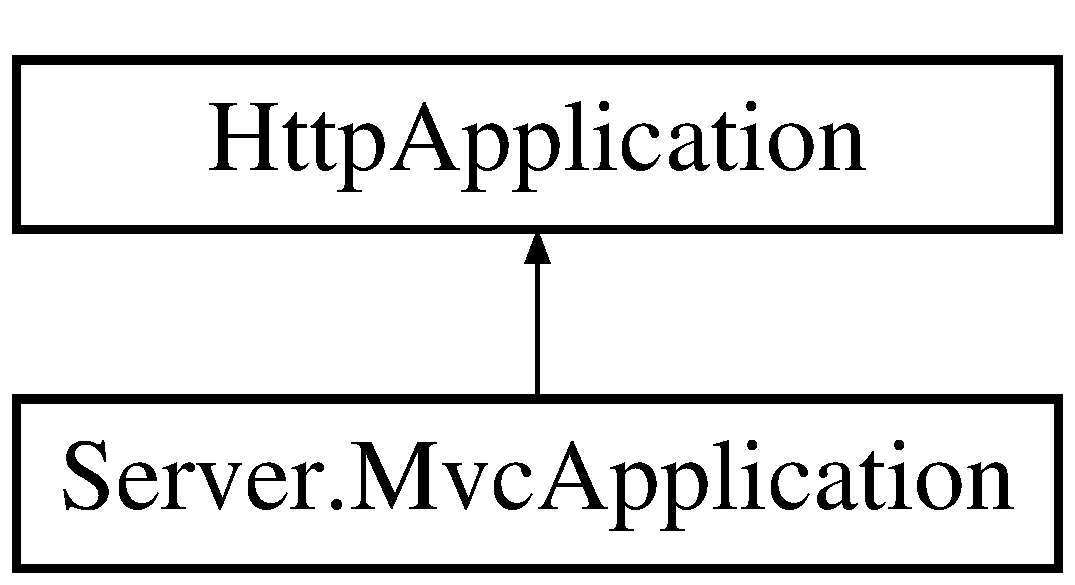
\includegraphics[height=2.000000cm]{classServer_1_1MvcApplication}
\end{center}
\end{figure}
\subsection*{Public Types}
\begin{DoxyCompactItemize}
\item 
enum {\bfseries Phases} \{ \\*
{\bfseries Started}, 
{\bfseries Init}, 
{\bfseries Running}, 
{\bfseries Pause}, 
\\*
{\bfseries Exit}
 \}
\end{DoxyCompactItemize}
\subsection*{Static Public Member Functions}
\begin{DoxyCompactItemize}
\item 
\hypertarget{classServer_1_1MvcApplication_a50dcfe940ddd423bded4a7e913ab9ccd}{static void {\bfseries Register\-Routes} (Route\-Collection routes)}\label{classServer_1_1MvcApplication_a50dcfe940ddd423bded4a7e913ab9ccd}

\item 
\hypertarget{classServer_1_1MvcApplication_ac65595dcc87fd3cebd1627e7f04ba04b}{static void {\bfseries Register\-Global\-Filters} (Global\-Filter\-Collection filters)}\label{classServer_1_1MvcApplication_ac65595dcc87fd3cebd1627e7f04ba04b}

\end{DoxyCompactItemize}
\subsection*{Static Public Attributes}
\begin{DoxyCompactItemize}
\item 
\hypertarget{classServer_1_1MvcApplication_aee00f1100bfc8ac1947093abe4d96f4c}{static Phases {\bfseries Phase} = Phases.\-Started}\label{classServer_1_1MvcApplication_aee00f1100bfc8ac1947093abe4d96f4c}

\end{DoxyCompactItemize}
\subsection*{Protected Member Functions}
\begin{DoxyCompactItemize}
\item 
\hypertarget{classServer_1_1MvcApplication_a31c9550b5dfb6c0949ba8b687169b18f}{void {\bfseries Application\-\_\-\-Start} ()}\label{classServer_1_1MvcApplication_a31c9550b5dfb6c0949ba8b687169b18f}

\end{DoxyCompactItemize}


The documentation for this class was generated from the following file\-:\begin{DoxyCompactItemize}
\item 
server/Global.\-asax.\-cs\end{DoxyCompactItemize}

\hypertarget{classClient_1_1Common_1_1Controllers_1_1NetworkController}{}\section{Client.\+Common.\+Controllers.\+Network\+Controller Class Reference}
\label{classClient_1_1Common_1_1Controllers_1_1NetworkController}\index{Client.\+Common.\+Controllers.\+Network\+Controller@{Client.\+Common.\+Controllers.\+Network\+Controller}}


the Network controller is a singleton to control the network up and download to the server.  


\subsection*{Public Member Functions}
\begin{DoxyCompactItemize}
\item 
async Task$<$ \hyperlink{classCore_1_1Models_1_1Definitions_1_1TerrainDefinition}{Terrain\+Definition}\mbox{[},\mbox{]}$>$ \hyperlink{classClient_1_1Common_1_1Controllers_1_1NetworkController_a5d45a3e5a8fcf0a755954d782af4e780}{Load\+Terrains\+Async} (\hyperlink{classCore_1_1Models_1_1RegionPosition}{Region\+Position} region\+Position)
\begin{DoxyCompactList}\small\item\em Loads the terrains async and returns it. \end{DoxyCompactList}\item 
async Task$<$ \hyperlink{classCore_1_1Models_1_1Definitions_1_1TerrainDefinition}{Core.\+Models.\+Definitions.\+Terrain\+Definition}\mbox{[}$\,$\mbox{]}$>$ \hyperlink{classClient_1_1Common_1_1Controllers_1_1NetworkController_a6e0ad22bc63585d4be358da45848063d}{Load\+Terrain\+Types\+Async} ()
\begin{DoxyCompactList}\small\item\em Loads the terrain types async and returns an array of Terrain\+Definition \end{DoxyCompactList}\item 
async Task$<$ \hyperlink{classCore_1_1Models_1_1Definitions_1_1UnitDefinition}{Core.\+Models.\+Definitions.\+Unit\+Definition}\mbox{[}$\,$\mbox{]}$>$ \hyperlink{classClient_1_1Common_1_1Controllers_1_1NetworkController_ab2e121298834c77bed8e204928fc21ff}{Load\+Unit\+Types\+Async} ()
\begin{DoxyCompactList}\small\item\em Loads the terrain types async and returns an array of Terrain\+Definition \end{DoxyCompactList}\item 
async Task$<$ \hyperlink{classCore_1_1Models_1_1Account}{Account} $>$ \hyperlink{classClient_1_1Common_1_1Controllers_1_1NetworkController_af3c0e3f5073dda246d20513013286919}{Login\+Async} (\hyperlink{classCore_1_1Models_1_1Position}{Core.\+Models.\+Position} current\+Game\+Position, string user, string password)
\begin{DoxyCompactList}\small\item\em Login async to the server and save the session\+I\+D. \end{DoxyCompactList}\item 
async Task$<$ \hyperlink{classCore_1_1Connections_1_1Response}{Core.\+Connections.\+Response} $>$ \hyperlink{classClient_1_1Common_1_1Controllers_1_1NetworkController_a27e260e1481b6ec9186915a9f64c3dce}{Load\+Entities\+Async} (\hyperlink{classCore_1_1Models_1_1Position}{Core.\+Models.\+Position} current\+Game\+Position, \hyperlink{classCore_1_1Models_1_1RegionPosition}{Region\+Position}\mbox{[}$\,$\mbox{]} region\+Positions)
\begin{DoxyCompactList}\small\item\em Loads the entities and actions async from the server. \end{DoxyCompactList}\item 
async Task$<$ bool $>$ \hyperlink{classClient_1_1Common_1_1Controllers_1_1NetworkController_a475c46ddb8c5dc4db7dea1530af9bf4b}{Do\+Actions\+Async} (\hyperlink{classCore_1_1Models_1_1Position}{Core.\+Models.\+Position} current\+Game\+Position, \hyperlink{classCore_1_1Models_1_1Action}{Core.\+Models.\+Action}\mbox{[}$\,$\mbox{]} actions)
\begin{DoxyCompactList}\small\item\em Sends the actions to the server. \end{DoxyCompactList}\end{DoxyCompactItemize}
\subsection*{Properties}
\begin{DoxyCompactItemize}
\item 
static \hyperlink{classClient_1_1Common_1_1Controllers_1_1NetworkController}{Network\+Controller} \hyperlink{classClient_1_1Common_1_1Controllers_1_1NetworkController_a24ad367082839e77f347f4a532d023ff}{Instance}\hspace{0.3cm}{\ttfamily  \mbox{[}get\mbox{]}}
\begin{DoxyCompactList}\small\item\em Gets the instance. \end{DoxyCompactList}\item 
bool \hyperlink{classClient_1_1Common_1_1Controllers_1_1NetworkController_afd2b5bdfc0da3720c3bbb257c0f73d94}{Is\+Logged\+In}\hspace{0.3cm}{\ttfamily  \mbox{[}get\mbox{]}}
\begin{DoxyCompactList}\small\item\em Gets a value indicating whether this instance is logged in . \end{DoxyCompactList}\end{DoxyCompactItemize}


\subsection{Detailed Description}
the Network controller is a singleton to control the network up and download to the server. 



\subsection{Member Function Documentation}
\hypertarget{classClient_1_1Common_1_1Controllers_1_1NetworkController_a475c46ddb8c5dc4db7dea1530af9bf4b}{}\index{Client\+::\+Common\+::\+Controllers\+::\+Network\+Controller@{Client\+::\+Common\+::\+Controllers\+::\+Network\+Controller}!Do\+Actions\+Async@{Do\+Actions\+Async}}
\index{Do\+Actions\+Async@{Do\+Actions\+Async}!Client\+::\+Common\+::\+Controllers\+::\+Network\+Controller@{Client\+::\+Common\+::\+Controllers\+::\+Network\+Controller}}
\subsubsection[{Do\+Actions\+Async(\+Core.\+Models.\+Position current\+Game\+Position, Core.\+Models.\+Action[] actions)}]{\setlength{\rightskip}{0pt plus 5cm}async Task$<$bool$>$ Client.\+Common.\+Controllers.\+Network\+Controller.\+Do\+Actions\+Async (
\begin{DoxyParamCaption}
\item[{{\bf Core.\+Models.\+Position}}]{current\+Game\+Position, }
\item[{{\bf Core.\+Models.\+Action}\mbox{[}$\,$\mbox{]}}]{actions}
\end{DoxyParamCaption}
)}\label{classClient_1_1Common_1_1Controllers_1_1NetworkController_a475c46ddb8c5dc4db7dea1530af9bf4b}


Sends the actions to the server. 

\begin{DoxyReturn}{Returns}
True if the response is ok, otherwise false.
\end{DoxyReturn}

\begin{DoxyParams}{Parameters}
{\em current\+Game\+Position} & Current game position.\\
\hline
{\em actions} & Actions which should be executed.\\
\hline
\end{DoxyParams}
\hypertarget{classClient_1_1Common_1_1Controllers_1_1NetworkController_a27e260e1481b6ec9186915a9f64c3dce}{}\index{Client\+::\+Common\+::\+Controllers\+::\+Network\+Controller@{Client\+::\+Common\+::\+Controllers\+::\+Network\+Controller}!Load\+Entities\+Async@{Load\+Entities\+Async}}
\index{Load\+Entities\+Async@{Load\+Entities\+Async}!Client\+::\+Common\+::\+Controllers\+::\+Network\+Controller@{Client\+::\+Common\+::\+Controllers\+::\+Network\+Controller}}
\subsubsection[{Load\+Entities\+Async(\+Core.\+Models.\+Position current\+Game\+Position, Region\+Position[] region\+Positions)}]{\setlength{\rightskip}{0pt plus 5cm}async Task$<${\bf Core.\+Connections.\+Response}$>$ Client.\+Common.\+Controllers.\+Network\+Controller.\+Load\+Entities\+Async (
\begin{DoxyParamCaption}
\item[{{\bf Core.\+Models.\+Position}}]{current\+Game\+Position, }
\item[{{\bf Region\+Position}\mbox{[}$\,$\mbox{]}}]{region\+Positions}
\end{DoxyParamCaption}
)}\label{classClient_1_1Common_1_1Controllers_1_1NetworkController_a27e260e1481b6ec9186915a9f64c3dce}


Loads the entities and actions async from the server. 

\begin{DoxyReturn}{Returns}
The entities response from the server.
\end{DoxyReturn}

\begin{DoxyParams}{Parameters}
{\em current\+Game\+Position} & Current game position.\\
\hline
{\em region\+Positions} & Region positions.\\
\hline
\end{DoxyParams}
\hypertarget{classClient_1_1Common_1_1Controllers_1_1NetworkController_a5d45a3e5a8fcf0a755954d782af4e780}{}\index{Client\+::\+Common\+::\+Controllers\+::\+Network\+Controller@{Client\+::\+Common\+::\+Controllers\+::\+Network\+Controller}!Load\+Terrains\+Async@{Load\+Terrains\+Async}}
\index{Load\+Terrains\+Async@{Load\+Terrains\+Async}!Client\+::\+Common\+::\+Controllers\+::\+Network\+Controller@{Client\+::\+Common\+::\+Controllers\+::\+Network\+Controller}}
\subsubsection[{Load\+Terrains\+Async(\+Region\+Position region\+Position)}]{\setlength{\rightskip}{0pt plus 5cm}async Task$<${\bf Terrain\+Definition}\mbox{[},\mbox{]}$>$ Client.\+Common.\+Controllers.\+Network\+Controller.\+Load\+Terrains\+Async (
\begin{DoxyParamCaption}
\item[{{\bf Region\+Position}}]{region\+Position}
\end{DoxyParamCaption}
)}\label{classClient_1_1Common_1_1Controllers_1_1NetworkController_a5d45a3e5a8fcf0a755954d782af4e780}


Loads the terrains async and returns it. 

\begin{DoxyReturn}{Returns}
The terrains async.
\end{DoxyReturn}

\begin{DoxyParams}{Parameters}
{\em region\+Position} & Region position.\\
\hline
\end{DoxyParams}
\hypertarget{classClient_1_1Common_1_1Controllers_1_1NetworkController_a6e0ad22bc63585d4be358da45848063d}{}\index{Client\+::\+Common\+::\+Controllers\+::\+Network\+Controller@{Client\+::\+Common\+::\+Controllers\+::\+Network\+Controller}!Load\+Terrain\+Types\+Async@{Load\+Terrain\+Types\+Async}}
\index{Load\+Terrain\+Types\+Async@{Load\+Terrain\+Types\+Async}!Client\+::\+Common\+::\+Controllers\+::\+Network\+Controller@{Client\+::\+Common\+::\+Controllers\+::\+Network\+Controller}}
\subsubsection[{Load\+Terrain\+Types\+Async()}]{\setlength{\rightskip}{0pt plus 5cm}async Task$<${\bf Core.\+Models.\+Definitions.\+Terrain\+Definition}\mbox{[}$\,$\mbox{]}$>$ Client.\+Common.\+Controllers.\+Network\+Controller.\+Load\+Terrain\+Types\+Async (
\begin{DoxyParamCaption}
{}
\end{DoxyParamCaption}
)}\label{classClient_1_1Common_1_1Controllers_1_1NetworkController_a6e0ad22bc63585d4be358da45848063d}


Loads the terrain types async and returns an array of Terrain\+Definition 

\begin{DoxyReturn}{Returns}
The terrain types async.
\end{DoxyReturn}
\hypertarget{classClient_1_1Common_1_1Controllers_1_1NetworkController_ab2e121298834c77bed8e204928fc21ff}{}\index{Client\+::\+Common\+::\+Controllers\+::\+Network\+Controller@{Client\+::\+Common\+::\+Controllers\+::\+Network\+Controller}!Load\+Unit\+Types\+Async@{Load\+Unit\+Types\+Async}}
\index{Load\+Unit\+Types\+Async@{Load\+Unit\+Types\+Async}!Client\+::\+Common\+::\+Controllers\+::\+Network\+Controller@{Client\+::\+Common\+::\+Controllers\+::\+Network\+Controller}}
\subsubsection[{Load\+Unit\+Types\+Async()}]{\setlength{\rightskip}{0pt plus 5cm}async Task$<${\bf Core.\+Models.\+Definitions.\+Unit\+Definition}\mbox{[}$\,$\mbox{]}$>$ Client.\+Common.\+Controllers.\+Network\+Controller.\+Load\+Unit\+Types\+Async (
\begin{DoxyParamCaption}
{}
\end{DoxyParamCaption}
)}\label{classClient_1_1Common_1_1Controllers_1_1NetworkController_ab2e121298834c77bed8e204928fc21ff}


Loads the terrain types async and returns an array of Terrain\+Definition 

\begin{DoxyReturn}{Returns}
The unit types async.
\end{DoxyReturn}
\hypertarget{classClient_1_1Common_1_1Controllers_1_1NetworkController_af3c0e3f5073dda246d20513013286919}{}\index{Client\+::\+Common\+::\+Controllers\+::\+Network\+Controller@{Client\+::\+Common\+::\+Controllers\+::\+Network\+Controller}!Login\+Async@{Login\+Async}}
\index{Login\+Async@{Login\+Async}!Client\+::\+Common\+::\+Controllers\+::\+Network\+Controller@{Client\+::\+Common\+::\+Controllers\+::\+Network\+Controller}}
\subsubsection[{Login\+Async(\+Core.\+Models.\+Position current\+Game\+Position, string user, string password)}]{\setlength{\rightskip}{0pt plus 5cm}async Task$<${\bf Account}$>$ Client.\+Common.\+Controllers.\+Network\+Controller.\+Login\+Async (
\begin{DoxyParamCaption}
\item[{{\bf Core.\+Models.\+Position}}]{current\+Game\+Position, }
\item[{string}]{user, }
\item[{string}]{password}
\end{DoxyParamCaption}
)}\label{classClient_1_1Common_1_1Controllers_1_1NetworkController_af3c0e3f5073dda246d20513013286919}


Login async to the server and save the session\+I\+D. 

\begin{DoxyReturn}{Returns}
The Account.
\end{DoxyReturn}

\begin{DoxyParams}{Parameters}
{\em current\+Game\+Position} & Current game position.\\
\hline
{\em user} & User which wanted to log in.\\
\hline
{\em password} & Password of the user.\\
\hline
\end{DoxyParams}


\subsection{Property Documentation}
\hypertarget{classClient_1_1Common_1_1Controllers_1_1NetworkController_a24ad367082839e77f347f4a532d023ff}{}\index{Client\+::\+Common\+::\+Controllers\+::\+Network\+Controller@{Client\+::\+Common\+::\+Controllers\+::\+Network\+Controller}!Instance@{Instance}}
\index{Instance@{Instance}!Client\+::\+Common\+::\+Controllers\+::\+Network\+Controller@{Client\+::\+Common\+::\+Controllers\+::\+Network\+Controller}}
\subsubsection[{Instance}]{\setlength{\rightskip}{0pt plus 5cm}{\bf Network\+Controller} Client.\+Common.\+Controllers.\+Network\+Controller.\+Instance\hspace{0.3cm}{\ttfamily [static]}, {\ttfamily [get]}}\label{classClient_1_1Common_1_1Controllers_1_1NetworkController_a24ad367082839e77f347f4a532d023ff}


Gets the instance. 

The instance.\hypertarget{classClient_1_1Common_1_1Controllers_1_1NetworkController_afd2b5bdfc0da3720c3bbb257c0f73d94}{}\index{Client\+::\+Common\+::\+Controllers\+::\+Network\+Controller@{Client\+::\+Common\+::\+Controllers\+::\+Network\+Controller}!Is\+Logged\+In@{Is\+Logged\+In}}
\index{Is\+Logged\+In@{Is\+Logged\+In}!Client\+::\+Common\+::\+Controllers\+::\+Network\+Controller@{Client\+::\+Common\+::\+Controllers\+::\+Network\+Controller}}
\subsubsection[{Is\+Logged\+In}]{\setlength{\rightskip}{0pt plus 5cm}bool Client.\+Common.\+Controllers.\+Network\+Controller.\+Is\+Logged\+In\hspace{0.3cm}{\ttfamily [get]}}\label{classClient_1_1Common_1_1Controllers_1_1NetworkController_afd2b5bdfc0da3720c3bbb257c0f73d94}


Gets a value indicating whether this instance is logged in . 

{\ttfamily true} if this instance is logged in; otherwise, {\ttfamily false}.

The documentation for this class was generated from the following file\+:\begin{DoxyCompactItemize}
\item 
client/client/client.\+Common/\+Controllers/Network\+Controller.\+cs\end{DoxyCompactItemize}

\hypertarget{classAStar_1_1Node}{\section{A\-Star.\-Node Class Reference}
\label{classAStar_1_1Node}\index{A\-Star.\-Node@{A\-Star.\-Node}}
}


Represents a single node on a grid that is being searched for a path between two points  


\subsection*{Public Member Functions}
\begin{DoxyCompactItemize}
\item 
\hyperlink{classAStar_1_1Node_a937f422d6e30afb82921967fdeb1a27b}{Node} (\hyperlink{classCore_1_1Models_1_1PositionI}{Position\-I} location, \hyperlink{classCore_1_1Models_1_1PositionI}{Position\-I} end\-Location)
\begin{DoxyCompactList}\small\item\em Constructor from a \hyperlink{classAStar_1_1Node}{Node}, it set the position\-I of the \hyperlink{classAStar_1_1Node}{Node}, set the nodstate to open and calculate the travel cost to the destination tile. \end{DoxyCompactList}\end{DoxyCompactItemize}
\subsection*{Public Attributes}
\begin{DoxyCompactItemize}
\item 
\hyperlink{namespaceAStar_a44d96e2d4066e21483fa07d62358c358}{Node\-State} \hyperlink{classAStar_1_1Node_a71d509fe94dee571f3852c9f60c63e13}{State}
\begin{DoxyCompactList}\small\item\em Flags whether the node is open, closed or untested by the \hyperlink{classAStar_1_1PathFinder}{Path\-Finder} \end{DoxyCompactList}\end{DoxyCompactItemize}
\subsection*{Properties}
\begin{DoxyCompactItemize}
\item 
\hyperlink{classCore_1_1Models_1_1PositionI}{Position\-I} \hyperlink{classAStar_1_1Node_afd917b94b45e7f39ebebb8b180bf16b5}{Location}\hspace{0.3cm}{\ttfamily  \mbox{[}get, set\mbox{]}}
\begin{DoxyCompactList}\small\item\em The node's location in the grid \end{DoxyCompactList}\item 
double \hyperlink{classAStar_1_1Node_ad35f9676be4b5d25936033f87a490d5d}{G}\hspace{0.3cm}{\ttfamily  \mbox{[}get, set\mbox{]}}
\begin{DoxyCompactList}\small\item\em Cost from start to here \end{DoxyCompactList}\item 
double \hyperlink{classAStar_1_1Node_ac396e73b68313b7402307f6f41da8179}{H}\hspace{0.3cm}{\ttfamily  \mbox{[}get, set\mbox{]}}
\begin{DoxyCompactList}\small\item\em Estimated cost from here to end \end{DoxyCompactList}\item 
double \hyperlink{classAStar_1_1Node_a2093196ab12b8969927bbd441f395558}{F}\hspace{0.3cm}{\ttfamily  \mbox{[}get\mbox{]}}
\begin{DoxyCompactList}\small\item\em Estimated total cost (F = G + H) \end{DoxyCompactList}\item 
\hyperlink{classAStar_1_1Node}{Node} \hyperlink{classAStar_1_1Node_af01de677cce55f979bab4ce6577c9614}{Parent\-Node}\hspace{0.3cm}{\ttfamily  \mbox{[}get, set\mbox{]}}
\begin{DoxyCompactList}\small\item\em Gets or sets the parent node. The start node's parent is always null. \end{DoxyCompactList}\end{DoxyCompactItemize}


\subsection{Detailed Description}
Represents a single node on a grid that is being searched for a path between two points 



\subsection{Constructor \& Destructor Documentation}
\hypertarget{classAStar_1_1Node_a937f422d6e30afb82921967fdeb1a27b}{\index{A\-Star\-::\-Node@{A\-Star\-::\-Node}!Node@{Node}}
\index{Node@{Node}!AStar::Node@{A\-Star\-::\-Node}}
\subsubsection[{Node}]{\setlength{\rightskip}{0pt plus 5cm}A\-Star.\-Node.\-Node (
\begin{DoxyParamCaption}
\item[{{\bf Position\-I}}]{location, }
\item[{{\bf Position\-I}}]{end\-Location}
\end{DoxyParamCaption}
)\hspace{0.3cm}{\ttfamily [inline]}}}\label{classAStar_1_1Node_a937f422d6e30afb82921967fdeb1a27b}


Constructor from a \hyperlink{classAStar_1_1Node}{Node}, it set the position\-I of the \hyperlink{classAStar_1_1Node}{Node}, set the nodstate to open and calculate the travel cost to the destination tile. 


\begin{DoxyParams}{Parameters}
{\em location} & Current postion\-I of the \hyperlink{classAStar_1_1Node}{Node}.\\
\hline
{\em end\-Location} & Position\-I of the destination tile.\\
\hline
\end{DoxyParams}


\subsection{Member Data Documentation}
\hypertarget{classAStar_1_1Node_a71d509fe94dee571f3852c9f60c63e13}{\index{A\-Star\-::\-Node@{A\-Star\-::\-Node}!State@{State}}
\index{State@{State}!AStar::Node@{A\-Star\-::\-Node}}
\subsubsection[{State}]{\setlength{\rightskip}{0pt plus 5cm}{\bf Node\-State} A\-Star.\-Node.\-State}}\label{classAStar_1_1Node_a71d509fe94dee571f3852c9f60c63e13}


Flags whether the node is open, closed or untested by the \hyperlink{classAStar_1_1PathFinder}{Path\-Finder} 



\subsection{Property Documentation}
\hypertarget{classAStar_1_1Node_a2093196ab12b8969927bbd441f395558}{\index{A\-Star\-::\-Node@{A\-Star\-::\-Node}!F@{F}}
\index{F@{F}!AStar::Node@{A\-Star\-::\-Node}}
\subsubsection[{F}]{\setlength{\rightskip}{0pt plus 5cm}double A\-Star.\-Node.\-F\hspace{0.3cm}{\ttfamily [get]}}}\label{classAStar_1_1Node_a2093196ab12b8969927bbd441f395558}


Estimated total cost (F = G + H) 

\hypertarget{classAStar_1_1Node_ad35f9676be4b5d25936033f87a490d5d}{\index{A\-Star\-::\-Node@{A\-Star\-::\-Node}!G@{G}}
\index{G@{G}!AStar::Node@{A\-Star\-::\-Node}}
\subsubsection[{G}]{\setlength{\rightskip}{0pt plus 5cm}double A\-Star.\-Node.\-G\hspace{0.3cm}{\ttfamily [get]}, {\ttfamily [set]}}}\label{classAStar_1_1Node_ad35f9676be4b5d25936033f87a490d5d}


Cost from start to here 

\hypertarget{classAStar_1_1Node_ac396e73b68313b7402307f6f41da8179}{\index{A\-Star\-::\-Node@{A\-Star\-::\-Node}!H@{H}}
\index{H@{H}!AStar::Node@{A\-Star\-::\-Node}}
\subsubsection[{H}]{\setlength{\rightskip}{0pt plus 5cm}double A\-Star.\-Node.\-H\hspace{0.3cm}{\ttfamily [get]}, {\ttfamily [set]}}}\label{classAStar_1_1Node_ac396e73b68313b7402307f6f41da8179}


Estimated cost from here to end 

\hypertarget{classAStar_1_1Node_afd917b94b45e7f39ebebb8b180bf16b5}{\index{A\-Star\-::\-Node@{A\-Star\-::\-Node}!Location@{Location}}
\index{Location@{Location}!AStar::Node@{A\-Star\-::\-Node}}
\subsubsection[{Location}]{\setlength{\rightskip}{0pt plus 5cm}{\bf Position\-I} A\-Star.\-Node.\-Location\hspace{0.3cm}{\ttfamily [get]}, {\ttfamily [set]}}}\label{classAStar_1_1Node_afd917b94b45e7f39ebebb8b180bf16b5}


The node's location in the grid 

\hypertarget{classAStar_1_1Node_af01de677cce55f979bab4ce6577c9614}{\index{A\-Star\-::\-Node@{A\-Star\-::\-Node}!Parent\-Node@{Parent\-Node}}
\index{Parent\-Node@{Parent\-Node}!AStar::Node@{A\-Star\-::\-Node}}
\subsubsection[{Parent\-Node}]{\setlength{\rightskip}{0pt plus 5cm}{\bf Node} A\-Star.\-Node.\-Parent\-Node\hspace{0.3cm}{\ttfamily [get]}, {\ttfamily [set]}}}\label{classAStar_1_1Node_af01de677cce55f979bab4ce6577c9614}


Gets or sets the parent node. The start node's parent is always null. 

The parent node.

The documentation for this class was generated from the following file\-:\begin{DoxyCompactItemize}
\item 
base/\-Controllers/\-Action/\-A\-Star/Node.\-cs\end{DoxyCompactItemize}

\hypertarget{classSQLite_1_1NotNullAttribute}{}\section{S\+Q\+Lite.\+Not\+Null\+Attribute Class Reference}
\label{classSQLite_1_1NotNullAttribute}\index{S\+Q\+Lite.\+Not\+Null\+Attribute@{S\+Q\+Lite.\+Not\+Null\+Attribute}}
Inheritance diagram for S\+Q\+Lite.\+Not\+Null\+Attribute\+:\begin{figure}[H]
\begin{center}
\leavevmode
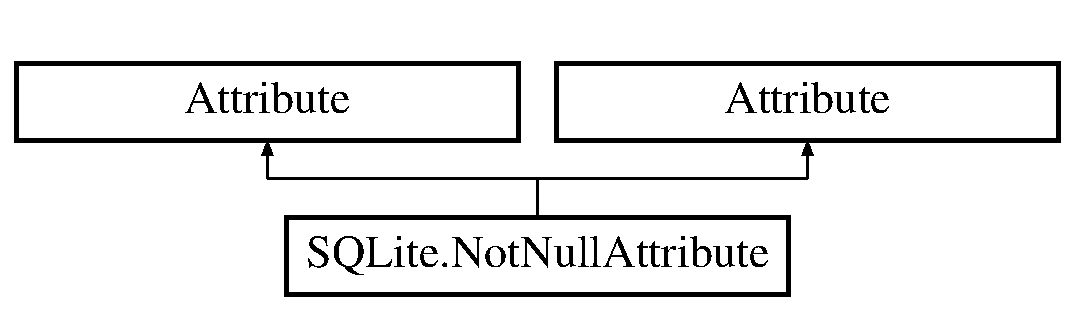
\includegraphics[height=2.000000cm]{classSQLite_1_1NotNullAttribute}
\end{center}
\end{figure}


The documentation for this class was generated from the following file\+:\begin{DoxyCompactItemize}
\item 
packages/sqlite-\/net.\+1.\+0.\+8/content/S\+Q\+Lite.\+cs\end{DoxyCompactItemize}

\hypertarget{classSQLite_1_1NotNullConstraintViolationException}{\section{S\-Q\-Lite.\-Not\-Null\-Constraint\-Violation\-Exception Class Reference}
\label{classSQLite_1_1NotNullConstraintViolationException}\index{S\-Q\-Lite.\-Not\-Null\-Constraint\-Violation\-Exception@{S\-Q\-Lite.\-Not\-Null\-Constraint\-Violation\-Exception}}
}
Inheritance diagram for S\-Q\-Lite.\-Not\-Null\-Constraint\-Violation\-Exception\-:\begin{figure}[H]
\begin{center}
\leavevmode
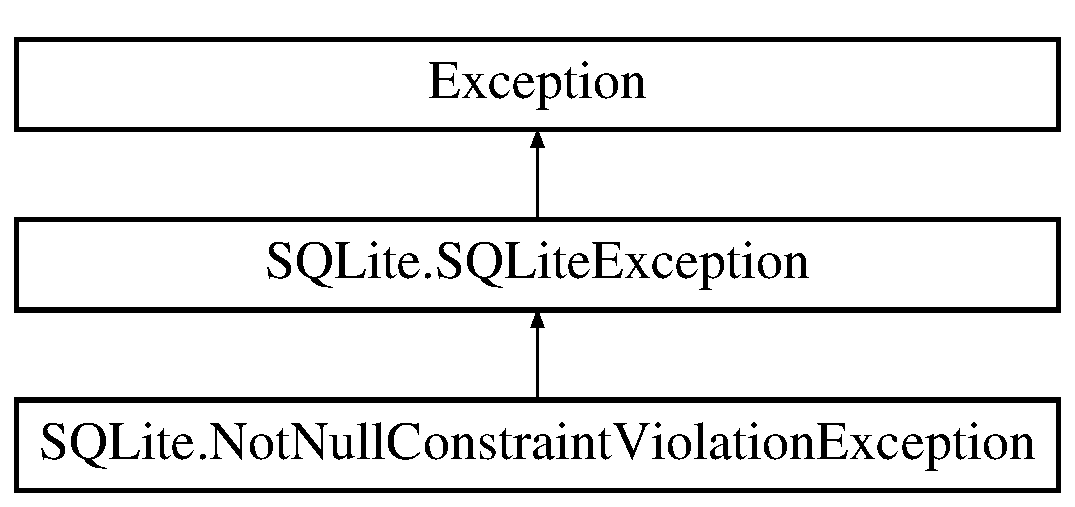
\includegraphics[height=1.590909cm]{classSQLite_1_1NotNullConstraintViolationException}
\end{center}
\end{figure}
\subsection*{Static Public Member Functions}
\begin{DoxyCompactItemize}
\item 
\hypertarget{classSQLite_1_1NotNullConstraintViolationException_a7989030e3242311aaca6b3d184184396}{static new \\*
\hyperlink{classSQLite_1_1NotNullConstraintViolationException}{Not\-Null\-Constraint\-Violation\-Exception} {\bfseries New} (S\-Q\-Lite3.\-Result r, string message)}\label{classSQLite_1_1NotNullConstraintViolationException_a7989030e3242311aaca6b3d184184396}

\item 
\hypertarget{classSQLite_1_1NotNullConstraintViolationException_ac25b33dde04a9b12bd6984038e4b2972}{static \\*
\hyperlink{classSQLite_1_1NotNullConstraintViolationException}{Not\-Null\-Constraint\-Violation\-Exception} {\bfseries New} (S\-Q\-Lite3.\-Result r, string message, \hyperlink{classSQLite_1_1TableMapping}{Table\-Mapping} mapping, object obj)}\label{classSQLite_1_1NotNullConstraintViolationException_ac25b33dde04a9b12bd6984038e4b2972}

\item 
\hypertarget{classSQLite_1_1NotNullConstraintViolationException_a25c290bafcea136ebd06b2959bf20c3c}{static \\*
\hyperlink{classSQLite_1_1NotNullConstraintViolationException}{Not\-Null\-Constraint\-Violation\-Exception} {\bfseries New} (\hyperlink{classSQLite_1_1SQLiteException}{S\-Q\-Lite\-Exception} exception, \hyperlink{classSQLite_1_1TableMapping}{Table\-Mapping} mapping, object obj)}\label{classSQLite_1_1NotNullConstraintViolationException_a25c290bafcea136ebd06b2959bf20c3c}

\item 
\hypertarget{classSQLite_1_1NotNullConstraintViolationException_a7989030e3242311aaca6b3d184184396}{static new \\*
\hyperlink{classSQLite_1_1NotNullConstraintViolationException}{Not\-Null\-Constraint\-Violation\-Exception} {\bfseries New} (S\-Q\-Lite3.\-Result r, string message)}\label{classSQLite_1_1NotNullConstraintViolationException_a7989030e3242311aaca6b3d184184396}

\item 
\hypertarget{classSQLite_1_1NotNullConstraintViolationException_ac25b33dde04a9b12bd6984038e4b2972}{static \\*
\hyperlink{classSQLite_1_1NotNullConstraintViolationException}{Not\-Null\-Constraint\-Violation\-Exception} {\bfseries New} (S\-Q\-Lite3.\-Result r, string message, \hyperlink{classSQLite_1_1TableMapping}{Table\-Mapping} mapping, object obj)}\label{classSQLite_1_1NotNullConstraintViolationException_ac25b33dde04a9b12bd6984038e4b2972}

\item 
\hypertarget{classSQLite_1_1NotNullConstraintViolationException_a25c290bafcea136ebd06b2959bf20c3c}{static \\*
\hyperlink{classSQLite_1_1NotNullConstraintViolationException}{Not\-Null\-Constraint\-Violation\-Exception} {\bfseries New} (\hyperlink{classSQLite_1_1SQLiteException}{S\-Q\-Lite\-Exception} exception, \hyperlink{classSQLite_1_1TableMapping}{Table\-Mapping} mapping, object obj)}\label{classSQLite_1_1NotNullConstraintViolationException_a25c290bafcea136ebd06b2959bf20c3c}

\end{DoxyCompactItemize}
\subsection*{Protected Member Functions}
\begin{DoxyCompactItemize}
\item 
\hypertarget{classSQLite_1_1NotNullConstraintViolationException_a6c1cdcfe9c9289aefb428bc42861a376}{{\bfseries Not\-Null\-Constraint\-Violation\-Exception} (S\-Q\-Lite3.\-Result r, string message)}\label{classSQLite_1_1NotNullConstraintViolationException_a6c1cdcfe9c9289aefb428bc42861a376}

\item 
\hypertarget{classSQLite_1_1NotNullConstraintViolationException_a1323d85e646b1eb71943d03619291677}{{\bfseries Not\-Null\-Constraint\-Violation\-Exception} (S\-Q\-Lite3.\-Result r, string message, \hyperlink{classSQLite_1_1TableMapping}{Table\-Mapping} mapping, object obj)}\label{classSQLite_1_1NotNullConstraintViolationException_a1323d85e646b1eb71943d03619291677}

\item 
\hypertarget{classSQLite_1_1NotNullConstraintViolationException_a6c1cdcfe9c9289aefb428bc42861a376}{{\bfseries Not\-Null\-Constraint\-Violation\-Exception} (S\-Q\-Lite3.\-Result r, string message)}\label{classSQLite_1_1NotNullConstraintViolationException_a6c1cdcfe9c9289aefb428bc42861a376}

\item 
\hypertarget{classSQLite_1_1NotNullConstraintViolationException_a1323d85e646b1eb71943d03619291677}{{\bfseries Not\-Null\-Constraint\-Violation\-Exception} (S\-Q\-Lite3.\-Result r, string message, \hyperlink{classSQLite_1_1TableMapping}{Table\-Mapping} mapping, object obj)}\label{classSQLite_1_1NotNullConstraintViolationException_a1323d85e646b1eb71943d03619291677}

\end{DoxyCompactItemize}
\subsection*{Properties}
\begin{DoxyCompactItemize}
\item 
\hypertarget{classSQLite_1_1NotNullConstraintViolationException_a3e68db16a1e55ac623c17205ad9e30dc}{I\-Enumerable$<$ \hyperlink{classSQLite_1_1TableMapping_1_1Column}{Table\-Mapping.\-Column} $>$ {\bfseries Columns}\hspace{0.3cm}{\ttfamily  \mbox{[}get, set\mbox{]}}}\label{classSQLite_1_1NotNullConstraintViolationException_a3e68db16a1e55ac623c17205ad9e30dc}

\end{DoxyCompactItemize}


The documentation for this class was generated from the following file\-:\begin{DoxyCompactItemize}
\item 
packages/sqlite-\/net.\-1.\-0.\-8/content/S\-Q\-Lite.\-cs\end{DoxyCompactItemize}

\hypertarget{classSQLite_1_1BaseTableQuery_1_1Ordering}{}\section{S\+Q\+Lite.\+Base\+Table\+Query.\+Ordering Class Reference}
\label{classSQLite_1_1BaseTableQuery_1_1Ordering}\index{S\+Q\+Lite.\+Base\+Table\+Query.\+Ordering@{S\+Q\+Lite.\+Base\+Table\+Query.\+Ordering}}
\subsection*{Properties}
\begin{DoxyCompactItemize}
\item 
\hypertarget{classSQLite_1_1BaseTableQuery_1_1Ordering_a4a73e6f27bb0b7b71672c2440f1e26d8}{}string {\bfseries Column\+Name}\hspace{0.3cm}{\ttfamily  \mbox{[}get, set\mbox{]}}\label{classSQLite_1_1BaseTableQuery_1_1Ordering_a4a73e6f27bb0b7b71672c2440f1e26d8}

\item 
\hypertarget{classSQLite_1_1BaseTableQuery_1_1Ordering_a6ac459a921405f8a577c64f70e615359}{}bool {\bfseries Ascending}\hspace{0.3cm}{\ttfamily  \mbox{[}get, set\mbox{]}}\label{classSQLite_1_1BaseTableQuery_1_1Ordering_a6ac459a921405f8a577c64f70e615359}

\end{DoxyCompactItemize}


The documentation for this class was generated from the following file\+:\begin{DoxyCompactItemize}
\item 
packages/sqlite-\/net.\+1.\+0.\+8/content/S\+Q\+Lite.\+cs\end{DoxyCompactItemize}

\hypertarget{classAStar_1_1PathFinder}{\section{A\-Star.\-Path\-Finder Class Reference}
\label{classAStar_1_1PathFinder}\index{A\-Star.\-Path\-Finder@{A\-Star.\-Path\-Finder}}
}


\href{http://blog.two-cats.com/2014/06/a-star-example/}{\tt http\-://blog.\-two-\/cats.\-com/2014/06/a-\/star-\/example/} founded by Mike Clift  


\subsection*{Public Member Functions}
\begin{DoxyCompactItemize}
\item 
\hyperlink{classAStar_1_1PathFinder_a56a02796dc128e54a9ff805dc1860ce3}{Path\-Finder} (\hyperlink{classAStar_1_1SearchParameters}{Search\-Parameters} search\-Parameters)
\begin{DoxyCompactList}\small\item\em Create a new instance of \hyperlink{classAStar_1_1PathFinder}{Path\-Finder} \end{DoxyCompactList}\item 
List$<$ \hyperlink{classCore_1_1Models_1_1PositionI}{Position\-I} $>$ \hyperlink{classAStar_1_1PathFinder_ab404a7887a779555af95a6e019e4b302}{Find\-Path} (int moves)
\begin{DoxyCompactList}\small\item\em Attempts to find a path from the start location to the end location based on the supplied \hyperlink{classAStar_1_1SearchParameters}{Search\-Parameters} \end{DoxyCompactList}\end{DoxyCompactItemize}


\subsection{Detailed Description}
\href{http://blog.two-cats.com/2014/06/a-star-example/}{\tt http\-://blog.\-two-\/cats.\-com/2014/06/a-\/star-\/example/} founded by Mike Clift 



\subsection{Constructor \& Destructor Documentation}
\hypertarget{classAStar_1_1PathFinder_a56a02796dc128e54a9ff805dc1860ce3}{\index{A\-Star\-::\-Path\-Finder@{A\-Star\-::\-Path\-Finder}!Path\-Finder@{Path\-Finder}}
\index{Path\-Finder@{Path\-Finder}!AStar::PathFinder@{A\-Star\-::\-Path\-Finder}}
\subsubsection[{Path\-Finder}]{\setlength{\rightskip}{0pt plus 5cm}A\-Star.\-Path\-Finder.\-Path\-Finder (
\begin{DoxyParamCaption}
\item[{{\bf Search\-Parameters}}]{search\-Parameters}
\end{DoxyParamCaption}
)\hspace{0.3cm}{\ttfamily [inline]}}}\label{classAStar_1_1PathFinder_a56a02796dc128e54a9ff805dc1860ce3}


Create a new instance of \hyperlink{classAStar_1_1PathFinder}{Path\-Finder} 


\begin{DoxyParams}{Parameters}
{\em search\-Parameters} & \\
\hline
\end{DoxyParams}


\subsection{Member Function Documentation}
\hypertarget{classAStar_1_1PathFinder_ab404a7887a779555af95a6e019e4b302}{\index{A\-Star\-::\-Path\-Finder@{A\-Star\-::\-Path\-Finder}!Find\-Path@{Find\-Path}}
\index{Find\-Path@{Find\-Path}!AStar::PathFinder@{A\-Star\-::\-Path\-Finder}}
\subsubsection[{Find\-Path}]{\setlength{\rightskip}{0pt plus 5cm}List$<${\bf Position\-I}$>$ A\-Star.\-Path\-Finder.\-Find\-Path (
\begin{DoxyParamCaption}
\item[{int}]{moves}
\end{DoxyParamCaption}
)\hspace{0.3cm}{\ttfamily [inline]}}}\label{classAStar_1_1PathFinder_ab404a7887a779555af95a6e019e4b302}


Attempts to find a path from the start location to the end location based on the supplied \hyperlink{classAStar_1_1SearchParameters}{Search\-Parameters} 

/// 
\begin{DoxyParams}{Parameters}
{\em moves} & \\
\hline
\end{DoxyParams}
\begin{DoxyReturn}{Returns}
A List of Points representing the path. If no path was found, the returned list is empty.
\end{DoxyReturn}


The documentation for this class was generated from the following file\-:\begin{DoxyCompactItemize}
\item 
base/\-Controllers/\-Action/\-A\-Star/Path\-Finder.\-cs\end{DoxyCompactItemize}

\hypertarget{classCore_1_1Models_1_1Position}{}\section{Core.\+Models.\+Position Class Reference}
\label{classCore_1_1Models_1_1Position}\index{Core.\+Models.\+Position@{Core.\+Models.\+Position}}


\hyperlink{classCore_1_1Models_1_1Position}{Position} in the Game\+World.  


\subsection*{Public Member Functions}
\begin{DoxyCompactItemize}
\item 
\hyperlink{classCore_1_1Models_1_1Position_ab6b49792138b5a0a22e13525acdacc9a}{Position} (double x, double y)
\begin{DoxyCompactList}\small\item\em Initializes a new instance of the \hyperlink{classCore_1_1Models_1_1Position}{Core.\+Models.\+Position} class. \end{DoxyCompactList}\item 
\hyperlink{classCore_1_1Models_1_1Position_a86b378bb7e6fbd16182fe0b169d23897}{Position} (\hyperlink{classCore_1_1Models_1_1PositionI}{Position\+I} position)
\begin{DoxyCompactList}\small\item\em Initializes a new instance of the \hyperlink{classCore_1_1Models_1_1Position}{Core.\+Models.\+Position} class. \end{DoxyCompactList}\item 
\hyperlink{classCore_1_1Models_1_1Position_a776d640b97d31e7460fe4a850299a4f0}{Position} (\hyperlink{classCore_1_1Models_1_1LatLon}{Lat\+Lon} lat\+Lon)
\begin{DoxyCompactList}\small\item\em Initializes a new instance of the \hyperlink{classCore_1_1Models_1_1Position}{Core.\+Models.\+Position} class. \end{DoxyCompactList}\item 
\hyperlink{classCore_1_1Models_1_1Position_a74d6d9f0c6f39849f0515b1c837fa2ef}{Position} (\hyperlink{classCore_1_1Models_1_1RegionPosition}{Region\+Position} region\+Position)
\begin{DoxyCompactList}\small\item\em Initializes a new instance of the \hyperlink{classCore_1_1Models_1_1Position}{Core.\+Models.\+Position} class. \end{DoxyCompactList}\item 
\hyperlink{classCore_1_1Models_1_1Position_a71cb4b1cddaf9ee97c7786089b2918ba}{Position} (\hyperlink{classCore_1_1Models_1_1RegionPosition}{Region\+Position} region\+Position, \hyperlink{classCore_1_1Models_1_1CellPosition}{Cell\+Position} cell\+Position)
\begin{DoxyCompactList}\small\item\em Initializes a new instance of the \hyperlink{classCore_1_1Models_1_1Position}{Core.\+Models.\+Position} class. \end{DoxyCompactList}\item 
\hyperlink{classCore_1_1Models_1_1Position_a7170355b2965f3a38403fc2e284b99b2}{Position} (int region\+Position\+X, int region\+Position\+Y, float cell\+Position\+X, float cell\+Position\+Y)
\begin{DoxyCompactList}\small\item\em Initializes a new instance of the \hyperlink{classCore_1_1Models_1_1Position}{Core.\+Models.\+Position} class. \end{DoxyCompactList}\item 
override bool \hyperlink{classCore_1_1Models_1_1Position_a1567fd4c36196e790e898fd510103d32}{Equals} (object obj)
\begin{DoxyCompactList}\small\item\em \hyperlink{namespaceTests}{Tests} two positions if they are the same. \end{DoxyCompactList}\item 
double \hyperlink{classCore_1_1Models_1_1Position_a705ea8b8d29426c30419c70d86d84921}{Distance} (\hyperlink{classCore_1_1Models_1_1Position}{Position} position)
\begin{DoxyCompactList}\small\item\em Distance from this to the specific position Warning\+: N\+O\+T R\+O\+O\+T\+E\+D. \end{DoxyCompactList}\item 
double \hyperlink{classCore_1_1Models_1_1Position_ac5995b654052669d462d54957b04e271}{Distance} (\hyperlink{classCore_1_1Models_1_1PositionI}{Position\+I} position)
\begin{DoxyCompactList}\small\item\em Distance from this to the specific position Warning\+: N\+O\+T R\+O\+O\+T\+E\+D. \end{DoxyCompactList}\end{DoxyCompactItemize}
\subsection*{Static Public Member Functions}
\begin{DoxyCompactItemize}
\item 
static \hyperlink{classCore_1_1Models_1_1Position}{Position} \hyperlink{classCore_1_1Models_1_1Position_aff986057eca807bf3007f6c007e3e0c2}{operator+} (\hyperlink{classCore_1_1Models_1_1Position}{Position} first, \hyperlink{classCore_1_1Models_1_1Position}{Position} second)
\begin{DoxyCompactList}\small\item\em Adds two positions. \end{DoxyCompactList}\item 
static \hyperlink{classCore_1_1Models_1_1Position}{Position} \hyperlink{classCore_1_1Models_1_1Position_afb344750ef4f2b476de90599c6fb9da4}{operator-\/} (\hyperlink{classCore_1_1Models_1_1Position}{Position} first, \hyperlink{classCore_1_1Models_1_1Position}{Position} second)
\begin{DoxyCompactList}\small\item\em Subtract second position from first position (first-\/second). \end{DoxyCompactList}\item 
static bool \hyperlink{classCore_1_1Models_1_1Position_ad4a08e9ecbdc1eeefd3a603372c42c22}{operator==} (\hyperlink{classCore_1_1Models_1_1Position}{Position} first, \hyperlink{classCore_1_1Models_1_1Position}{Position} second)
\begin{DoxyCompactList}\small\item\em \hyperlink{namespaceTests}{Tests} two positions if they are the same. \end{DoxyCompactList}\item 
static bool \hyperlink{classCore_1_1Models_1_1Position_a509b4347ca7f125c97449701409c9f0e}{operator!=} (\hyperlink{classCore_1_1Models_1_1Position}{Position} first, \hyperlink{classCore_1_1Models_1_1Position}{Position} second)
\begin{DoxyCompactList}\small\item\em \hyperlink{namespaceTests}{Tests} two positions if they are N\+O\+T the same. \end{DoxyCompactList}\end{DoxyCompactItemize}
\subsection*{Properties}
\begin{DoxyCompactItemize}
\item 
double \hyperlink{classCore_1_1Models_1_1Position_a60f236378b77fb83a9b51d92c5d4359f}{X}\hspace{0.3cm}{\ttfamily  \mbox{[}get\mbox{]}}
\begin{DoxyCompactList}\small\item\em Gets the x. \end{DoxyCompactList}\item 
double \hyperlink{classCore_1_1Models_1_1Position_a795b40cbfc260e222c319cd50b5ab78c}{Y}\hspace{0.3cm}{\ttfamily  \mbox{[}get\mbox{]}}
\begin{DoxyCompactList}\small\item\em Gets the y. \end{DoxyCompactList}\item 
\hyperlink{classCore_1_1Models_1_1RegionPosition}{Region\+Position} \hyperlink{classCore_1_1Models_1_1Position_a7b92c9b041328e5f660f1a9f137249c6}{Region\+Position}\hspace{0.3cm}{\ttfamily  \mbox{[}get\mbox{]}}
\begin{DoxyCompactList}\small\item\em Gets the region position. \end{DoxyCompactList}\item 
\hyperlink{classCore_1_1Models_1_1CellPosition}{Cell\+Position} \hyperlink{classCore_1_1Models_1_1Position_afee231a72dbd2f57329e2bdd2fbc25bb}{Cell\+Position}\hspace{0.3cm}{\ttfamily  \mbox{[}get\mbox{]}}
\begin{DoxyCompactList}\small\item\em Gets the cell position. \end{DoxyCompactList}\end{DoxyCompactItemize}


\subsection{Detailed Description}
\hyperlink{classCore_1_1Models_1_1Position}{Position} in the Game\+World. 



\subsection{Constructor \& Destructor Documentation}
\hypertarget{classCore_1_1Models_1_1Position_ab6b49792138b5a0a22e13525acdacc9a}{}\index{Core\+::\+Models\+::\+Position@{Core\+::\+Models\+::\+Position}!Position@{Position}}
\index{Position@{Position}!Core\+::\+Models\+::\+Position@{Core\+::\+Models\+::\+Position}}
\subsubsection[{Position(double x, double y)}]{\setlength{\rightskip}{0pt plus 5cm}Core.\+Models.\+Position.\+Position (
\begin{DoxyParamCaption}
\item[{double}]{x, }
\item[{double}]{y}
\end{DoxyParamCaption}
)}\label{classCore_1_1Models_1_1Position_ab6b49792138b5a0a22e13525acdacc9a}


Initializes a new instance of the \hyperlink{classCore_1_1Models_1_1Position}{Core.\+Models.\+Position} class. 


\begin{DoxyParams}{Parameters}
{\em x} & The x coordinate.\\
\hline
{\em y} & The y coordinate.\\
\hline
\end{DoxyParams}
\hypertarget{classCore_1_1Models_1_1Position_a86b378bb7e6fbd16182fe0b169d23897}{}\index{Core\+::\+Models\+::\+Position@{Core\+::\+Models\+::\+Position}!Position@{Position}}
\index{Position@{Position}!Core\+::\+Models\+::\+Position@{Core\+::\+Models\+::\+Position}}
\subsubsection[{Position(\+Position\+I position)}]{\setlength{\rightskip}{0pt plus 5cm}Core.\+Models.\+Position.\+Position (
\begin{DoxyParamCaption}
\item[{{\bf Position\+I}}]{position}
\end{DoxyParamCaption}
)}\label{classCore_1_1Models_1_1Position_a86b378bb7e6fbd16182fe0b169d23897}


Initializes a new instance of the \hyperlink{classCore_1_1Models_1_1Position}{Core.\+Models.\+Position} class. 


\begin{DoxyParams}{Parameters}
{\em position} & \hyperlink{classCore_1_1Models_1_1Position}{Position} in X and Y.\\
\hline
\end{DoxyParams}
\hypertarget{classCore_1_1Models_1_1Position_a776d640b97d31e7460fe4a850299a4f0}{}\index{Core\+::\+Models\+::\+Position@{Core\+::\+Models\+::\+Position}!Position@{Position}}
\index{Position@{Position}!Core\+::\+Models\+::\+Position@{Core\+::\+Models\+::\+Position}}
\subsubsection[{Position(\+Lat\+Lon lat\+Lon)}]{\setlength{\rightskip}{0pt plus 5cm}Core.\+Models.\+Position.\+Position (
\begin{DoxyParamCaption}
\item[{{\bf Lat\+Lon}}]{lat\+Lon}
\end{DoxyParamCaption}
)}\label{classCore_1_1Models_1_1Position_a776d640b97d31e7460fe4a850299a4f0}


Initializes a new instance of the \hyperlink{classCore_1_1Models_1_1Position}{Core.\+Models.\+Position} class. 


\begin{DoxyParams}{Parameters}
{\em lat\+Lon} & Latitude longitude.\\
\hline
\end{DoxyParams}
\hypertarget{classCore_1_1Models_1_1Position_a74d6d9f0c6f39849f0515b1c837fa2ef}{}\index{Core\+::\+Models\+::\+Position@{Core\+::\+Models\+::\+Position}!Position@{Position}}
\index{Position@{Position}!Core\+::\+Models\+::\+Position@{Core\+::\+Models\+::\+Position}}
\subsubsection[{Position(\+Region\+Position region\+Position)}]{\setlength{\rightskip}{0pt plus 5cm}Core.\+Models.\+Position.\+Position (
\begin{DoxyParamCaption}
\item[{{\bf Region\+Position}}]{region\+Position}
\end{DoxyParamCaption}
)}\label{classCore_1_1Models_1_1Position_a74d6d9f0c6f39849f0515b1c837fa2ef}


Initializes a new instance of the \hyperlink{classCore_1_1Models_1_1Position}{Core.\+Models.\+Position} class. 


\begin{DoxyParams}{Parameters}
{\em region\+Position} & \hyperlink{classCore_1_1Models_1_1Region}{Region} position.\\
\hline
\end{DoxyParams}
\hypertarget{classCore_1_1Models_1_1Position_a71cb4b1cddaf9ee97c7786089b2918ba}{}\index{Core\+::\+Models\+::\+Position@{Core\+::\+Models\+::\+Position}!Position@{Position}}
\index{Position@{Position}!Core\+::\+Models\+::\+Position@{Core\+::\+Models\+::\+Position}}
\subsubsection[{Position(\+Region\+Position region\+Position, Cell\+Position cell\+Position)}]{\setlength{\rightskip}{0pt plus 5cm}Core.\+Models.\+Position.\+Position (
\begin{DoxyParamCaption}
\item[{{\bf Region\+Position}}]{region\+Position, }
\item[{{\bf Cell\+Position}}]{cell\+Position}
\end{DoxyParamCaption}
)}\label{classCore_1_1Models_1_1Position_a71cb4b1cddaf9ee97c7786089b2918ba}


Initializes a new instance of the \hyperlink{classCore_1_1Models_1_1Position}{Core.\+Models.\+Position} class. 


\begin{DoxyParams}{Parameters}
{\em region\+Position} & \hyperlink{classCore_1_1Models_1_1Region}{Region} position.\\
\hline
{\em cell\+Position} & Cell position.\\
\hline
\end{DoxyParams}
\hypertarget{classCore_1_1Models_1_1Position_a7170355b2965f3a38403fc2e284b99b2}{}\index{Core\+::\+Models\+::\+Position@{Core\+::\+Models\+::\+Position}!Position@{Position}}
\index{Position@{Position}!Core\+::\+Models\+::\+Position@{Core\+::\+Models\+::\+Position}}
\subsubsection[{Position(int region\+Position\+X, int region\+Position\+Y, float cell\+Position\+X, float cell\+Position\+Y)}]{\setlength{\rightskip}{0pt plus 5cm}Core.\+Models.\+Position.\+Position (
\begin{DoxyParamCaption}
\item[{int}]{region\+Position\+X, }
\item[{int}]{region\+Position\+Y, }
\item[{float}]{cell\+Position\+X, }
\item[{float}]{cell\+Position\+Y}
\end{DoxyParamCaption}
)}\label{classCore_1_1Models_1_1Position_a7170355b2965f3a38403fc2e284b99b2}


Initializes a new instance of the \hyperlink{classCore_1_1Models_1_1Position}{Core.\+Models.\+Position} class. 


\begin{DoxyParams}{Parameters}
{\em region\+Position\+X} & \hyperlink{classCore_1_1Models_1_1Region}{Region} position x.\\
\hline
{\em region\+Position\+Y} & \hyperlink{classCore_1_1Models_1_1Region}{Region} position y.\\
\hline
{\em cell\+Position\+X} & Cell position x.\\
\hline
{\em cell\+Position\+Y} & Cell position y.\\
\hline
\end{DoxyParams}


\subsection{Member Function Documentation}
\hypertarget{classCore_1_1Models_1_1Position_a705ea8b8d29426c30419c70d86d84921}{}\index{Core\+::\+Models\+::\+Position@{Core\+::\+Models\+::\+Position}!Distance@{Distance}}
\index{Distance@{Distance}!Core\+::\+Models\+::\+Position@{Core\+::\+Models\+::\+Position}}
\subsubsection[{Distance(\+Position position)}]{\setlength{\rightskip}{0pt plus 5cm}double Core.\+Models.\+Position.\+Distance (
\begin{DoxyParamCaption}
\item[{{\bf Position}}]{position}
\end{DoxyParamCaption}
)}\label{classCore_1_1Models_1_1Position_a705ea8b8d29426c30419c70d86d84921}


Distance from this to the specific position Warning\+: N\+O\+T R\+O\+O\+T\+E\+D. 

\begin{DoxyReturn}{Returns}
Distance from this to the specific position.
\end{DoxyReturn}

\begin{DoxyParams}{Parameters}
{\em position} & Other \hyperlink{classCore_1_1Models_1_1Position}{Position}.\\
\hline
\end{DoxyParams}
\hypertarget{classCore_1_1Models_1_1Position_ac5995b654052669d462d54957b04e271}{}\index{Core\+::\+Models\+::\+Position@{Core\+::\+Models\+::\+Position}!Distance@{Distance}}
\index{Distance@{Distance}!Core\+::\+Models\+::\+Position@{Core\+::\+Models\+::\+Position}}
\subsubsection[{Distance(\+Position\+I position)}]{\setlength{\rightskip}{0pt plus 5cm}double Core.\+Models.\+Position.\+Distance (
\begin{DoxyParamCaption}
\item[{{\bf Position\+I}}]{position}
\end{DoxyParamCaption}
)}\label{classCore_1_1Models_1_1Position_ac5995b654052669d462d54957b04e271}


Distance from this to the specific position Warning\+: N\+O\+T R\+O\+O\+T\+E\+D. 

\begin{DoxyReturn}{Returns}
Distance from this to the specific position.
\end{DoxyReturn}

\begin{DoxyParams}{Parameters}
{\em position} & Other \hyperlink{classCore_1_1Models_1_1Position}{Position}.\\
\hline
\end{DoxyParams}
\hypertarget{classCore_1_1Models_1_1Position_a1567fd4c36196e790e898fd510103d32}{}\index{Core\+::\+Models\+::\+Position@{Core\+::\+Models\+::\+Position}!Equals@{Equals}}
\index{Equals@{Equals}!Core\+::\+Models\+::\+Position@{Core\+::\+Models\+::\+Position}}
\subsubsection[{Equals(object obj)}]{\setlength{\rightskip}{0pt plus 5cm}override bool Core.\+Models.\+Position.\+Equals (
\begin{DoxyParamCaption}
\item[{object}]{obj}
\end{DoxyParamCaption}
)}\label{classCore_1_1Models_1_1Position_a1567fd4c36196e790e898fd510103d32}


\hyperlink{namespaceTests}{Tests} two positions if they are the same. 

\begin{DoxyReturn}{Returns}
boolean if both position are the same. Otherwise false.
\end{DoxyReturn}

\begin{DoxyParams}{Parameters}
{\em obj} & The System.\+Object to compare with the current \hyperlink{classCore_1_1Models_1_1Position}{Core.\+Models.\+Position}.\\
\hline
\end{DoxyParams}
\hypertarget{classCore_1_1Models_1_1Position_a509b4347ca7f125c97449701409c9f0e}{}\index{Core\+::\+Models\+::\+Position@{Core\+::\+Models\+::\+Position}!operator"!=@{operator"!=}}
\index{operator"!=@{operator"!=}!Core\+::\+Models\+::\+Position@{Core\+::\+Models\+::\+Position}}
\subsubsection[{operator"!=(\+Position first, Position second)}]{\setlength{\rightskip}{0pt plus 5cm}static bool Core.\+Models.\+Position.\+operator!= (
\begin{DoxyParamCaption}
\item[{{\bf Position}}]{first, }
\item[{{\bf Position}}]{second}
\end{DoxyParamCaption}
)\hspace{0.3cm}{\ttfamily [static]}}\label{classCore_1_1Models_1_1Position_a509b4347ca7f125c97449701409c9f0e}


\hyperlink{namespaceTests}{Tests} two positions if they are N\+O\+T the same. 

\begin{DoxyReturn}{Returns}
boolean if both position are N\+O\+T the same. Otherwise false.
\end{DoxyReturn}

\begin{DoxyParams}{Parameters}
{\em first} & First position.\\
\hline
{\em second} & Second position.\\
\hline
\end{DoxyParams}
\hypertarget{classCore_1_1Models_1_1Position_aff986057eca807bf3007f6c007e3e0c2}{}\index{Core\+::\+Models\+::\+Position@{Core\+::\+Models\+::\+Position}!operator+@{operator+}}
\index{operator+@{operator+}!Core\+::\+Models\+::\+Position@{Core\+::\+Models\+::\+Position}}
\subsubsection[{operator+(\+Position first, Position second)}]{\setlength{\rightskip}{0pt plus 5cm}static {\bf Position} Core.\+Models.\+Position.\+operator+ (
\begin{DoxyParamCaption}
\item[{{\bf Position}}]{first, }
\item[{{\bf Position}}]{second}
\end{DoxyParamCaption}
)\hspace{0.3cm}{\ttfamily [static]}}\label{classCore_1_1Models_1_1Position_aff986057eca807bf3007f6c007e3e0c2}


Adds two positions. 

\begin{DoxyReturn}{Returns}
Resulted \hyperlink{classCore_1_1Models_1_1Position}{Position}
\end{DoxyReturn}

\begin{DoxyParams}{Parameters}
{\em first} & First \hyperlink{classCore_1_1Models_1_1Position}{Position}.\\
\hline
{\em second} & Second \hyperlink{classCore_1_1Models_1_1Position}{Position}.\\
\hline
\end{DoxyParams}
\hypertarget{classCore_1_1Models_1_1Position_afb344750ef4f2b476de90599c6fb9da4}{}\index{Core\+::\+Models\+::\+Position@{Core\+::\+Models\+::\+Position}!operator-\/@{operator-\/}}
\index{operator-\/@{operator-\/}!Core\+::\+Models\+::\+Position@{Core\+::\+Models\+::\+Position}}
\subsubsection[{operator-\/(\+Position first, Position second)}]{\setlength{\rightskip}{0pt plus 5cm}static {\bf Position} Core.\+Models.\+Position.\+operator-\/ (
\begin{DoxyParamCaption}
\item[{{\bf Position}}]{first, }
\item[{{\bf Position}}]{second}
\end{DoxyParamCaption}
)\hspace{0.3cm}{\ttfamily [static]}}\label{classCore_1_1Models_1_1Position_afb344750ef4f2b476de90599c6fb9da4}


Subtract second position from first position (first-\/second). 

\begin{DoxyReturn}{Returns}
Resulted \hyperlink{classCore_1_1Models_1_1Position}{Position}
\end{DoxyReturn}

\begin{DoxyParams}{Parameters}
{\em first} & First \hyperlink{classCore_1_1Models_1_1Position}{Position}.\\
\hline
{\em second} & Second \hyperlink{classCore_1_1Models_1_1Position}{Position}.\\
\hline
\end{DoxyParams}
\hypertarget{classCore_1_1Models_1_1Position_ad4a08e9ecbdc1eeefd3a603372c42c22}{}\index{Core\+::\+Models\+::\+Position@{Core\+::\+Models\+::\+Position}!operator==@{operator==}}
\index{operator==@{operator==}!Core\+::\+Models\+::\+Position@{Core\+::\+Models\+::\+Position}}
\subsubsection[{operator==(\+Position first, Position second)}]{\setlength{\rightskip}{0pt plus 5cm}static bool Core.\+Models.\+Position.\+operator== (
\begin{DoxyParamCaption}
\item[{{\bf Position}}]{first, }
\item[{{\bf Position}}]{second}
\end{DoxyParamCaption}
)\hspace{0.3cm}{\ttfamily [static]}}\label{classCore_1_1Models_1_1Position_ad4a08e9ecbdc1eeefd3a603372c42c22}


\hyperlink{namespaceTests}{Tests} two positions if they are the same. 

\begin{DoxyReturn}{Returns}
boolean if both position are the same. Otherwise false.
\end{DoxyReturn}

\begin{DoxyParams}{Parameters}
{\em first} & First \hyperlink{classCore_1_1Models_1_1Position}{Position}.\\
\hline
{\em second} & Second \hyperlink{classCore_1_1Models_1_1Position}{Position}.\\
\hline
\end{DoxyParams}


\subsection{Property Documentation}
\hypertarget{classCore_1_1Models_1_1Position_afee231a72dbd2f57329e2bdd2fbc25bb}{}\index{Core\+::\+Models\+::\+Position@{Core\+::\+Models\+::\+Position}!Cell\+Position@{Cell\+Position}}
\index{Cell\+Position@{Cell\+Position}!Core\+::\+Models\+::\+Position@{Core\+::\+Models\+::\+Position}}
\subsubsection[{Cell\+Position}]{\setlength{\rightskip}{0pt plus 5cm}{\bf Cell\+Position} Core.\+Models.\+Position.\+Cell\+Position\hspace{0.3cm}{\ttfamily [get]}}\label{classCore_1_1Models_1_1Position_afee231a72dbd2f57329e2bdd2fbc25bb}


Gets the cell position. 

The cell position.\hypertarget{classCore_1_1Models_1_1Position_a7b92c9b041328e5f660f1a9f137249c6}{}\index{Core\+::\+Models\+::\+Position@{Core\+::\+Models\+::\+Position}!Region\+Position@{Region\+Position}}
\index{Region\+Position@{Region\+Position}!Core\+::\+Models\+::\+Position@{Core\+::\+Models\+::\+Position}}
\subsubsection[{Region\+Position}]{\setlength{\rightskip}{0pt plus 5cm}{\bf Region\+Position} Core.\+Models.\+Position.\+Region\+Position\hspace{0.3cm}{\ttfamily [get]}}\label{classCore_1_1Models_1_1Position_a7b92c9b041328e5f660f1a9f137249c6}


Gets the region position. 

The region position.\hypertarget{classCore_1_1Models_1_1Position_a60f236378b77fb83a9b51d92c5d4359f}{}\index{Core\+::\+Models\+::\+Position@{Core\+::\+Models\+::\+Position}!X@{X}}
\index{X@{X}!Core\+::\+Models\+::\+Position@{Core\+::\+Models\+::\+Position}}
\subsubsection[{X}]{\setlength{\rightskip}{0pt plus 5cm}double Core.\+Models.\+Position.\+X\hspace{0.3cm}{\ttfamily [get]}}\label{classCore_1_1Models_1_1Position_a60f236378b77fb83a9b51d92c5d4359f}


Gets the x. 

The x.\hypertarget{classCore_1_1Models_1_1Position_a795b40cbfc260e222c319cd50b5ab78c}{}\index{Core\+::\+Models\+::\+Position@{Core\+::\+Models\+::\+Position}!Y@{Y}}
\index{Y@{Y}!Core\+::\+Models\+::\+Position@{Core\+::\+Models\+::\+Position}}
\subsubsection[{Y}]{\setlength{\rightskip}{0pt plus 5cm}double Core.\+Models.\+Position.\+Y\hspace{0.3cm}{\ttfamily [get]}}\label{classCore_1_1Models_1_1Position_a795b40cbfc260e222c319cd50b5ab78c}


Gets the y. 

The y.

The documentation for this class was generated from the following file\+:\begin{DoxyCompactItemize}
\item 
base/\+Models/\+Position/Position.\+cs\end{DoxyCompactItemize}

\hypertarget{classClient_1_1Common_1_1Helper_1_1PositionHelper}{\section{Client.\-Common.\-Helper.\-Position\-Helper Class Reference}
\label{classClient_1_1Common_1_1Helper_1_1PositionHelper}\index{Client.\-Common.\-Helper.\-Position\-Helper@{Client.\-Common.\-Helper.\-Position\-Helper}}
}
\subsection*{Static Public Member Functions}
\begin{DoxyCompactItemize}
\item 
\hypertarget{classClient_1_1Common_1_1Helper_1_1PositionHelper_ac77b450a32ee660ee2c141cecbc08c0c}{static \\*
Cocos\-Sharp.\-C\-C\-Tile\-Map\-Coordinates {\bfseries Position\-To\-Tile\-Map\-Coordinates} (\hyperlink{classCore_1_1Models_1_1Position}{Position} center\-Position, \hyperlink{classCore_1_1Models_1_1PositionI}{Position\-I} position)}\label{classClient_1_1Common_1_1Helper_1_1PositionHelper_ac77b450a32ee660ee2c141cecbc08c0c}

\item 
\hypertarget{classClient_1_1Common_1_1Helper_1_1PositionHelper_af2ba9ab8c3c50e5f41ba5f4cd65ca013}{static \hyperlink{classClient_1_1Common_1_1Models_1_1MapCellPosition}{Map\-Cell\-Position} {\bfseries Position\-To\-Map\-Cell\-Position} (\hyperlink{classCore_1_1Models_1_1Position}{Position} center\-Position, \hyperlink{classCore_1_1Models_1_1PositionI}{Position\-I} position)}\label{classClient_1_1Common_1_1Helper_1_1PositionHelper_af2ba9ab8c3c50e5f41ba5f4cd65ca013}

\end{DoxyCompactItemize}


The documentation for this class was generated from the following file\-:\begin{DoxyCompactItemize}
\item 
client/client/client.\-Common/\-Helper/Position\-Helper.\-cs\end{DoxyCompactItemize}

\hypertarget{classCore_1_1Models_1_1PositionI}{}\section{Core.\+Models.\+Position\+I Class Reference}
\label{classCore_1_1Models_1_1PositionI}\index{Core.\+Models.\+Position\+I@{Core.\+Models.\+Position\+I}}


\hyperlink{classCore_1_1Models_1_1Position}{Position} in the Game world as Integer (so it is discrete). Can be used to identify one field in the \hyperlink{classCore_1_1Models_1_1World}{World}.  


\subsection*{Public Member Functions}
\begin{DoxyCompactItemize}
\item 
\hyperlink{classCore_1_1Models_1_1PositionI_a77a350d1cd0431b7640fc50c2d1f1b08}{Position\+I} (int x, int y)
\begin{DoxyCompactList}\small\item\em Initializes a new instance of the \hyperlink{classCore_1_1Models_1_1PositionI}{Core.\+Models.\+Position\+I} class. \end{DoxyCompactList}\item 
\hyperlink{classCore_1_1Models_1_1PositionI_aa96d094d9d0c73b95ed5e3bcc3c7139c}{Position\+I} (J\+Container obj)
\begin{DoxyCompactList}\small\item\em Initializes a new instance of the \hyperlink{classCore_1_1Models_1_1PositionI}{Core.\+Models.\+Position\+I} class. \end{DoxyCompactList}\item 
\hyperlink{classCore_1_1Models_1_1PositionI_a754155c0d79a76caa5175332f7cb87f4}{Position\+I} (\hyperlink{classCore_1_1Models_1_1RegionPosition}{Region\+Position} region\+Position, \hyperlink{classCore_1_1Models_1_1CellPosition}{Cell\+Position} cell\+Position)
\begin{DoxyCompactList}\small\item\em Initializes a new instance of the \hyperlink{classCore_1_1Models_1_1PositionI}{Core.\+Models.\+Position\+I} class. \end{DoxyCompactList}\item 
\hyperlink{classCore_1_1Models_1_1PositionI_a7ae2d0db70f2e9273cfa3a5c9ff24bc7}{Position\+I} (\hyperlink{classCore_1_1Models_1_1Position}{Position} position)
\begin{DoxyCompactList}\small\item\em Initializes a new instance of the \hyperlink{classCore_1_1Models_1_1PositionI}{Core.\+Models.\+Position\+I} class. \end{DoxyCompactList}\item 
override int \hyperlink{classCore_1_1Models_1_1PositionI_a082277a73568d67195014709867621c4}{Get\+Hash\+Code} ()
\begin{DoxyCompactList}\small\item\em Standard hash function \end{DoxyCompactList}\item 
override bool \hyperlink{classCore_1_1Models_1_1PositionI_a369069ed29555fd908a4a94df50d0543}{Equals} (object obj)
\begin{DoxyCompactList}\small\item\em tests if the given object is equal to this object. \end{DoxyCompactList}\item 
double \hyperlink{classCore_1_1Models_1_1PositionI_ae0f397e10a3daa4cbe2b2103018bb3b0}{Distance} (\hyperlink{classCore_1_1Models_1_1PositionI}{Position\+I} position)
\begin{DoxyCompactList}\small\item\em Distance from this to the specific position Warning\+: N\+O\+T R\+O\+O\+T\+E\+D. \end{DoxyCompactList}\item 
double \hyperlink{classCore_1_1Models_1_1PositionI_af02949d6124b593a75f9dcb947d89dce}{Distance} (\hyperlink{classCore_1_1Models_1_1Position}{Position} position)
\begin{DoxyCompactList}\small\item\em Distance from this to the specific position Warning\+: N\+O\+T R\+O\+O\+T\+E\+D. \end{DoxyCompactList}\end{DoxyCompactItemize}
\subsection*{Static Public Member Functions}
\begin{DoxyCompactItemize}
\item 
static \hyperlink{classCore_1_1Models_1_1PositionI}{Position\+I} \hyperlink{classCore_1_1Models_1_1PositionI_a0217783ab1b5749b63e61bc56f407812}{operator+} (\hyperlink{classCore_1_1Models_1_1PositionI}{Position\+I} first, \hyperlink{classCore_1_1Models_1_1PositionI}{Position\+I} second)
\begin{DoxyCompactList}\small\item\em Adds two positions. \end{DoxyCompactList}\item 
static \hyperlink{classCore_1_1Models_1_1PositionI}{Position\+I} \hyperlink{classCore_1_1Models_1_1PositionI_aadbefbad3c41a124e4adc6c5895ccd0f}{operator-\/} (\hyperlink{classCore_1_1Models_1_1PositionI}{Position\+I} first, \hyperlink{classCore_1_1Models_1_1PositionI}{Position\+I} second)
\begin{DoxyCompactList}\small\item\em Subtract second position from first position (first-\/second). \end{DoxyCompactList}\item 
static bool \hyperlink{classCore_1_1Models_1_1PositionI_a43fff439645b1ce32c9ba087ed9db53c}{operator==} (\hyperlink{classCore_1_1Models_1_1PositionI}{Position\+I} first, \hyperlink{classCore_1_1Models_1_1PositionI}{Position\+I} second)
\begin{DoxyCompactList}\small\item\em \hyperlink{namespaceTests}{Tests} two positions if they are the same. \end{DoxyCompactList}\item 
static bool \hyperlink{classCore_1_1Models_1_1PositionI_a3243525ef665f9aaf5b0dcab58300b27}{operator!=} (\hyperlink{classCore_1_1Models_1_1PositionI}{Position\+I} first, \hyperlink{classCore_1_1Models_1_1PositionI}{Position\+I} second)
\begin{DoxyCompactList}\small\item\em \hyperlink{namespaceTests}{Tests} two positions if they are N\+O\+T the same. \end{DoxyCompactList}\end{DoxyCompactItemize}
\subsection*{Properties}
\begin{DoxyCompactItemize}
\item 
\hyperlink{classCore_1_1Models_1_1RegionPosition}{Region\+Position} \hyperlink{classCore_1_1Models_1_1PositionI_a0662e0b43f175a5320f043298984659b}{Region\+Position}\hspace{0.3cm}{\ttfamily  \mbox{[}get\mbox{]}}
\begin{DoxyCompactList}\small\item\em Gets the region position. \end{DoxyCompactList}\item 
\hyperlink{classCore_1_1Models_1_1CellPosition}{Cell\+Position} \hyperlink{classCore_1_1Models_1_1PositionI_a205a6a5cdd2e73781c2adf0b370402a9}{Cell\+Position}\hspace{0.3cm}{\ttfamily  \mbox{[}get\mbox{]}}
\begin{DoxyCompactList}\small\item\em Gets the cell position. \end{DoxyCompactList}\item 
int \hyperlink{classCore_1_1Models_1_1PositionI_a2612b865ceba85b37714a5d19a0228c5}{X}\hspace{0.3cm}{\ttfamily  \mbox{[}get\mbox{]}}
\begin{DoxyCompactList}\small\item\em Gets the x. \end{DoxyCompactList}\item 
int \hyperlink{classCore_1_1Models_1_1PositionI_ae8a742f3f984a83b3fc7706a2c9ed254}{Y}\hspace{0.3cm}{\ttfamily  \mbox{[}get\mbox{]}}
\begin{DoxyCompactList}\small\item\em Gets the y. \end{DoxyCompactList}\end{DoxyCompactItemize}


\subsection{Detailed Description}
\hyperlink{classCore_1_1Models_1_1Position}{Position} in the Game world as Integer (so it is discrete). Can be used to identify one field in the \hyperlink{classCore_1_1Models_1_1World}{World}. 



\subsection{Constructor \& Destructor Documentation}
\hypertarget{classCore_1_1Models_1_1PositionI_a77a350d1cd0431b7640fc50c2d1f1b08}{}\index{Core\+::\+Models\+::\+Position\+I@{Core\+::\+Models\+::\+Position\+I}!Position\+I@{Position\+I}}
\index{Position\+I@{Position\+I}!Core\+::\+Models\+::\+Position\+I@{Core\+::\+Models\+::\+Position\+I}}
\subsubsection[{Position\+I(int x, int y)}]{\setlength{\rightskip}{0pt plus 5cm}Core.\+Models.\+Position\+I.\+Position\+I (
\begin{DoxyParamCaption}
\item[{int}]{x, }
\item[{int}]{y}
\end{DoxyParamCaption}
)}\label{classCore_1_1Models_1_1PositionI_a77a350d1cd0431b7640fc50c2d1f1b08}


Initializes a new instance of the \hyperlink{classCore_1_1Models_1_1PositionI}{Core.\+Models.\+Position\+I} class. 


\begin{DoxyParams}{Parameters}
{\em x} & The x coordinate.\\
\hline
{\em y} & The y coordinate.\\
\hline
\end{DoxyParams}
\hypertarget{classCore_1_1Models_1_1PositionI_aa96d094d9d0c73b95ed5e3bcc3c7139c}{}\index{Core\+::\+Models\+::\+Position\+I@{Core\+::\+Models\+::\+Position\+I}!Position\+I@{Position\+I}}
\index{Position\+I@{Position\+I}!Core\+::\+Models\+::\+Position\+I@{Core\+::\+Models\+::\+Position\+I}}
\subsubsection[{Position\+I(\+J\+Container obj)}]{\setlength{\rightskip}{0pt plus 5cm}Core.\+Models.\+Position\+I.\+Position\+I (
\begin{DoxyParamCaption}
\item[{J\+Container}]{obj}
\end{DoxyParamCaption}
)}\label{classCore_1_1Models_1_1PositionI_aa96d094d9d0c73b95ed5e3bcc3c7139c}


Initializes a new instance of the \hyperlink{classCore_1_1Models_1_1PositionI}{Core.\+Models.\+Position\+I} class. 


\begin{DoxyParams}{Parameters}
{\em obj} & J\+S\+O\+N Object.\\
\hline
\end{DoxyParams}
\hypertarget{classCore_1_1Models_1_1PositionI_a754155c0d79a76caa5175332f7cb87f4}{}\index{Core\+::\+Models\+::\+Position\+I@{Core\+::\+Models\+::\+Position\+I}!Position\+I@{Position\+I}}
\index{Position\+I@{Position\+I}!Core\+::\+Models\+::\+Position\+I@{Core\+::\+Models\+::\+Position\+I}}
\subsubsection[{Position\+I(\+Region\+Position region\+Position, Cell\+Position cell\+Position)}]{\setlength{\rightskip}{0pt plus 5cm}Core.\+Models.\+Position\+I.\+Position\+I (
\begin{DoxyParamCaption}
\item[{{\bf Region\+Position}}]{region\+Position, }
\item[{{\bf Cell\+Position}}]{cell\+Position}
\end{DoxyParamCaption}
)}\label{classCore_1_1Models_1_1PositionI_a754155c0d79a76caa5175332f7cb87f4}


Initializes a new instance of the \hyperlink{classCore_1_1Models_1_1PositionI}{Core.\+Models.\+Position\+I} class. 


\begin{DoxyParams}{Parameters}
{\em region\+Position} & \hyperlink{classCore_1_1Models_1_1Region}{Region} position.\\
\hline
{\em cell\+Position} & Cell position.\\
\hline
\end{DoxyParams}
\hypertarget{classCore_1_1Models_1_1PositionI_a7ae2d0db70f2e9273cfa3a5c9ff24bc7}{}\index{Core\+::\+Models\+::\+Position\+I@{Core\+::\+Models\+::\+Position\+I}!Position\+I@{Position\+I}}
\index{Position\+I@{Position\+I}!Core\+::\+Models\+::\+Position\+I@{Core\+::\+Models\+::\+Position\+I}}
\subsubsection[{Position\+I(\+Position position)}]{\setlength{\rightskip}{0pt plus 5cm}Core.\+Models.\+Position\+I.\+Position\+I (
\begin{DoxyParamCaption}
\item[{{\bf Position}}]{position}
\end{DoxyParamCaption}
)}\label{classCore_1_1Models_1_1PositionI_a7ae2d0db70f2e9273cfa3a5c9ff24bc7}


Initializes a new instance of the \hyperlink{classCore_1_1Models_1_1PositionI}{Core.\+Models.\+Position\+I} class. 


\begin{DoxyParams}{Parameters}
{\em position} & \hyperlink{classCore_1_1Models_1_1Position}{Position} which should be copied.\\
\hline
\end{DoxyParams}


\subsection{Member Function Documentation}
\hypertarget{classCore_1_1Models_1_1PositionI_ae0f397e10a3daa4cbe2b2103018bb3b0}{}\index{Core\+::\+Models\+::\+Position\+I@{Core\+::\+Models\+::\+Position\+I}!Distance@{Distance}}
\index{Distance@{Distance}!Core\+::\+Models\+::\+Position\+I@{Core\+::\+Models\+::\+Position\+I}}
\subsubsection[{Distance(\+Position\+I position)}]{\setlength{\rightskip}{0pt plus 5cm}double Core.\+Models.\+Position\+I.\+Distance (
\begin{DoxyParamCaption}
\item[{{\bf Position\+I}}]{position}
\end{DoxyParamCaption}
)}\label{classCore_1_1Models_1_1PositionI_ae0f397e10a3daa4cbe2b2103018bb3b0}


Distance from this to the specific position Warning\+: N\+O\+T R\+O\+O\+T\+E\+D. 

\begin{DoxyReturn}{Returns}
Distance from this to the specific position.
\end{DoxyReturn}

\begin{DoxyParams}{Parameters}
{\em position} & Other \hyperlink{classCore_1_1Models_1_1Position}{Position}.\\
\hline
\end{DoxyParams}
\hypertarget{classCore_1_1Models_1_1PositionI_af02949d6124b593a75f9dcb947d89dce}{}\index{Core\+::\+Models\+::\+Position\+I@{Core\+::\+Models\+::\+Position\+I}!Distance@{Distance}}
\index{Distance@{Distance}!Core\+::\+Models\+::\+Position\+I@{Core\+::\+Models\+::\+Position\+I}}
\subsubsection[{Distance(\+Position position)}]{\setlength{\rightskip}{0pt plus 5cm}double Core.\+Models.\+Position\+I.\+Distance (
\begin{DoxyParamCaption}
\item[{{\bf Position}}]{position}
\end{DoxyParamCaption}
)}\label{classCore_1_1Models_1_1PositionI_af02949d6124b593a75f9dcb947d89dce}


Distance from this to the specific position Warning\+: N\+O\+T R\+O\+O\+T\+E\+D. 

\begin{DoxyReturn}{Returns}
Distance from this to the specific position.
\end{DoxyReturn}

\begin{DoxyParams}{Parameters}
{\em position} & Other \hyperlink{classCore_1_1Models_1_1Position}{Position}.\\
\hline
\end{DoxyParams}
\hypertarget{classCore_1_1Models_1_1PositionI_a369069ed29555fd908a4a94df50d0543}{}\index{Core\+::\+Models\+::\+Position\+I@{Core\+::\+Models\+::\+Position\+I}!Equals@{Equals}}
\index{Equals@{Equals}!Core\+::\+Models\+::\+Position\+I@{Core\+::\+Models\+::\+Position\+I}}
\subsubsection[{Equals(object obj)}]{\setlength{\rightskip}{0pt plus 5cm}override bool Core.\+Models.\+Position\+I.\+Equals (
\begin{DoxyParamCaption}
\item[{object}]{obj}
\end{DoxyParamCaption}
)}\label{classCore_1_1Models_1_1PositionI_a369069ed29555fd908a4a94df50d0543}


tests if the given object is equal to this object. 

\begin{DoxyReturn}{Returns}
true, if both objects are equal, otherwise false.
\end{DoxyReturn}

\begin{DoxyParams}{Parameters}
{\em obj} & The System.\+Object to compare with the current \hyperlink{classCore_1_1Models_1_1PositionI}{Core.\+Models.\+Position\+I}.\\
\hline
\end{DoxyParams}
\hypertarget{classCore_1_1Models_1_1PositionI_a082277a73568d67195014709867621c4}{}\index{Core\+::\+Models\+::\+Position\+I@{Core\+::\+Models\+::\+Position\+I}!Get\+Hash\+Code@{Get\+Hash\+Code}}
\index{Get\+Hash\+Code@{Get\+Hash\+Code}!Core\+::\+Models\+::\+Position\+I@{Core\+::\+Models\+::\+Position\+I}}
\subsubsection[{Get\+Hash\+Code()}]{\setlength{\rightskip}{0pt plus 5cm}override int Core.\+Models.\+Position\+I.\+Get\+Hash\+Code (
\begin{DoxyParamCaption}
{}
\end{DoxyParamCaption}
)}\label{classCore_1_1Models_1_1PositionI_a082277a73568d67195014709867621c4}


Standard hash function 

\begin{DoxyReturn}{Returns}
Hash code.
\end{DoxyReturn}
\hypertarget{classCore_1_1Models_1_1PositionI_a3243525ef665f9aaf5b0dcab58300b27}{}\index{Core\+::\+Models\+::\+Position\+I@{Core\+::\+Models\+::\+Position\+I}!operator"!=@{operator"!=}}
\index{operator"!=@{operator"!=}!Core\+::\+Models\+::\+Position\+I@{Core\+::\+Models\+::\+Position\+I}}
\subsubsection[{operator"!=(\+Position\+I first, Position\+I second)}]{\setlength{\rightskip}{0pt plus 5cm}static bool Core.\+Models.\+Position\+I.\+operator!= (
\begin{DoxyParamCaption}
\item[{{\bf Position\+I}}]{first, }
\item[{{\bf Position\+I}}]{second}
\end{DoxyParamCaption}
)\hspace{0.3cm}{\ttfamily [static]}}\label{classCore_1_1Models_1_1PositionI_a3243525ef665f9aaf5b0dcab58300b27}


\hyperlink{namespaceTests}{Tests} two positions if they are N\+O\+T the same. 

\begin{DoxyReturn}{Returns}
boolean if both position are N\+O\+T the same. Otherwise false.
\end{DoxyReturn}

\begin{DoxyParams}{Parameters}
{\em first} & First position.\\
\hline
{\em second} & Second position.\\
\hline
\end{DoxyParams}
\hypertarget{classCore_1_1Models_1_1PositionI_a0217783ab1b5749b63e61bc56f407812}{}\index{Core\+::\+Models\+::\+Position\+I@{Core\+::\+Models\+::\+Position\+I}!operator+@{operator+}}
\index{operator+@{operator+}!Core\+::\+Models\+::\+Position\+I@{Core\+::\+Models\+::\+Position\+I}}
\subsubsection[{operator+(\+Position\+I first, Position\+I second)}]{\setlength{\rightskip}{0pt plus 5cm}static {\bf Position\+I} Core.\+Models.\+Position\+I.\+operator+ (
\begin{DoxyParamCaption}
\item[{{\bf Position\+I}}]{first, }
\item[{{\bf Position\+I}}]{second}
\end{DoxyParamCaption}
)\hspace{0.3cm}{\ttfamily [static]}}\label{classCore_1_1Models_1_1PositionI_a0217783ab1b5749b63e61bc56f407812}


Adds two positions. 

\begin{DoxyReturn}{Returns}
Resulted \hyperlink{classCore_1_1Models_1_1Position}{Position}
\end{DoxyReturn}

\begin{DoxyParams}{Parameters}
{\em first} & First \hyperlink{classCore_1_1Models_1_1Position}{Position}.\\
\hline
{\em second} & Second \hyperlink{classCore_1_1Models_1_1Position}{Position}.\\
\hline
\end{DoxyParams}
\hypertarget{classCore_1_1Models_1_1PositionI_aadbefbad3c41a124e4adc6c5895ccd0f}{}\index{Core\+::\+Models\+::\+Position\+I@{Core\+::\+Models\+::\+Position\+I}!operator-\/@{operator-\/}}
\index{operator-\/@{operator-\/}!Core\+::\+Models\+::\+Position\+I@{Core\+::\+Models\+::\+Position\+I}}
\subsubsection[{operator-\/(\+Position\+I first, Position\+I second)}]{\setlength{\rightskip}{0pt plus 5cm}static {\bf Position\+I} Core.\+Models.\+Position\+I.\+operator-\/ (
\begin{DoxyParamCaption}
\item[{{\bf Position\+I}}]{first, }
\item[{{\bf Position\+I}}]{second}
\end{DoxyParamCaption}
)\hspace{0.3cm}{\ttfamily [static]}}\label{classCore_1_1Models_1_1PositionI_aadbefbad3c41a124e4adc6c5895ccd0f}


Subtract second position from first position (first-\/second). 

\begin{DoxyReturn}{Returns}
Resulted \hyperlink{classCore_1_1Models_1_1Position}{Position}
\end{DoxyReturn}

\begin{DoxyParams}{Parameters}
{\em first} & First \hyperlink{classCore_1_1Models_1_1Position}{Position}.\\
\hline
{\em second} & Second \hyperlink{classCore_1_1Models_1_1Position}{Position}.\\
\hline
\end{DoxyParams}
\hypertarget{classCore_1_1Models_1_1PositionI_a43fff439645b1ce32c9ba087ed9db53c}{}\index{Core\+::\+Models\+::\+Position\+I@{Core\+::\+Models\+::\+Position\+I}!operator==@{operator==}}
\index{operator==@{operator==}!Core\+::\+Models\+::\+Position\+I@{Core\+::\+Models\+::\+Position\+I}}
\subsubsection[{operator==(\+Position\+I first, Position\+I second)}]{\setlength{\rightskip}{0pt plus 5cm}static bool Core.\+Models.\+Position\+I.\+operator== (
\begin{DoxyParamCaption}
\item[{{\bf Position\+I}}]{first, }
\item[{{\bf Position\+I}}]{second}
\end{DoxyParamCaption}
)\hspace{0.3cm}{\ttfamily [static]}}\label{classCore_1_1Models_1_1PositionI_a43fff439645b1ce32c9ba087ed9db53c}


\hyperlink{namespaceTests}{Tests} two positions if they are the same. 

\begin{DoxyReturn}{Returns}
boolean if both position are the same. Otherwise false.
\end{DoxyReturn}

\begin{DoxyParams}{Parameters}
{\em first} & First \hyperlink{classCore_1_1Models_1_1Position}{Position}.\\
\hline
{\em second} & Second \hyperlink{classCore_1_1Models_1_1Position}{Position}.\\
\hline
\end{DoxyParams}


\subsection{Property Documentation}
\hypertarget{classCore_1_1Models_1_1PositionI_a205a6a5cdd2e73781c2adf0b370402a9}{}\index{Core\+::\+Models\+::\+Position\+I@{Core\+::\+Models\+::\+Position\+I}!Cell\+Position@{Cell\+Position}}
\index{Cell\+Position@{Cell\+Position}!Core\+::\+Models\+::\+Position\+I@{Core\+::\+Models\+::\+Position\+I}}
\subsubsection[{Cell\+Position}]{\setlength{\rightskip}{0pt plus 5cm}{\bf Cell\+Position} Core.\+Models.\+Position\+I.\+Cell\+Position\hspace{0.3cm}{\ttfamily [get]}}\label{classCore_1_1Models_1_1PositionI_a205a6a5cdd2e73781c2adf0b370402a9}


Gets the cell position. 

The cell position.\hypertarget{classCore_1_1Models_1_1PositionI_a0662e0b43f175a5320f043298984659b}{}\index{Core\+::\+Models\+::\+Position\+I@{Core\+::\+Models\+::\+Position\+I}!Region\+Position@{Region\+Position}}
\index{Region\+Position@{Region\+Position}!Core\+::\+Models\+::\+Position\+I@{Core\+::\+Models\+::\+Position\+I}}
\subsubsection[{Region\+Position}]{\setlength{\rightskip}{0pt plus 5cm}{\bf Region\+Position} Core.\+Models.\+Position\+I.\+Region\+Position\hspace{0.3cm}{\ttfamily [get]}}\label{classCore_1_1Models_1_1PositionI_a0662e0b43f175a5320f043298984659b}


Gets the region position. 

The region position.\hypertarget{classCore_1_1Models_1_1PositionI_a2612b865ceba85b37714a5d19a0228c5}{}\index{Core\+::\+Models\+::\+Position\+I@{Core\+::\+Models\+::\+Position\+I}!X@{X}}
\index{X@{X}!Core\+::\+Models\+::\+Position\+I@{Core\+::\+Models\+::\+Position\+I}}
\subsubsection[{X}]{\setlength{\rightskip}{0pt plus 5cm}int Core.\+Models.\+Position\+I.\+X\hspace{0.3cm}{\ttfamily [get]}}\label{classCore_1_1Models_1_1PositionI_a2612b865ceba85b37714a5d19a0228c5}


Gets the x. 

The x.\hypertarget{classCore_1_1Models_1_1PositionI_ae8a742f3f984a83b3fc7706a2c9ed254}{}\index{Core\+::\+Models\+::\+Position\+I@{Core\+::\+Models\+::\+Position\+I}!Y@{Y}}
\index{Y@{Y}!Core\+::\+Models\+::\+Position\+I@{Core\+::\+Models\+::\+Position\+I}}
\subsubsection[{Y}]{\setlength{\rightskip}{0pt plus 5cm}int Core.\+Models.\+Position\+I.\+Y\hspace{0.3cm}{\ttfamily [get]}}\label{classCore_1_1Models_1_1PositionI_ae8a742f3f984a83b3fc7706a2c9ed254}


Gets the y. 

The y.

The documentation for this class was generated from the following file\+:\begin{DoxyCompactItemize}
\item 
base/\+Models/\+Position/Position\+I.\+cs\end{DoxyCompactItemize}

\hypertarget{classSQLite_1_1PreparedSqlLiteInsertCommand}{\section{S\-Q\-Lite.\-Prepared\-Sql\-Lite\-Insert\-Command Class Reference}
\label{classSQLite_1_1PreparedSqlLiteInsertCommand}\index{S\-Q\-Lite.\-Prepared\-Sql\-Lite\-Insert\-Command@{S\-Q\-Lite.\-Prepared\-Sql\-Lite\-Insert\-Command}}
}


Since the insert never changed, we only need to prepare once.  


Inheritance diagram for S\-Q\-Lite.\-Prepared\-Sql\-Lite\-Insert\-Command\-:\begin{figure}[H]
\begin{center}
\leavevmode
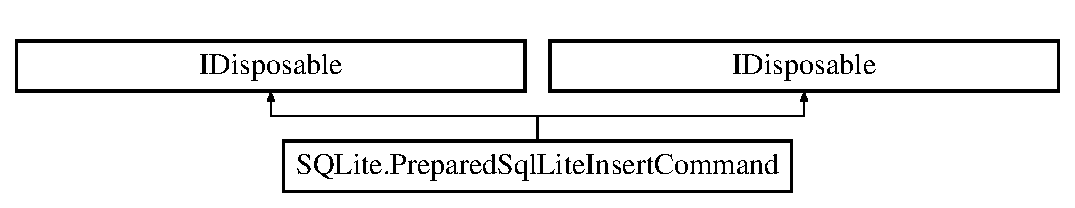
\includegraphics[height=2.000000cm]{classSQLite_1_1PreparedSqlLiteInsertCommand}
\end{center}
\end{figure}
\subsection*{Public Member Functions}
\begin{DoxyCompactItemize}
\item 
\hypertarget{classSQLite_1_1PreparedSqlLiteInsertCommand_a9f95629a1b978710741c23129d78fccc}{int {\bfseries Execute\-Non\-Query} (object\mbox{[}$\,$\mbox{]} source)}\label{classSQLite_1_1PreparedSqlLiteInsertCommand_a9f95629a1b978710741c23129d78fccc}

\item 
\hypertarget{classSQLite_1_1PreparedSqlLiteInsertCommand_a4569b8fb13658e105658b073937efead}{void {\bfseries Dispose} ()}\label{classSQLite_1_1PreparedSqlLiteInsertCommand_a4569b8fb13658e105658b073937efead}

\item 
\hypertarget{classSQLite_1_1PreparedSqlLiteInsertCommand_a9f95629a1b978710741c23129d78fccc}{int {\bfseries Execute\-Non\-Query} (object\mbox{[}$\,$\mbox{]} source)}\label{classSQLite_1_1PreparedSqlLiteInsertCommand_a9f95629a1b978710741c23129d78fccc}

\item 
\hypertarget{classSQLite_1_1PreparedSqlLiteInsertCommand_a4569b8fb13658e105658b073937efead}{void {\bfseries Dispose} ()}\label{classSQLite_1_1PreparedSqlLiteInsertCommand_a4569b8fb13658e105658b073937efead}

\end{DoxyCompactItemize}
\subsection*{Protected Member Functions}
\begin{DoxyCompactItemize}
\item 
\hypertarget{classSQLite_1_1PreparedSqlLiteInsertCommand_a207353ff88c74bc45cb076fe3cf463bb}{virtual Sqlite3\-Statement {\bfseries Prepare} ()}\label{classSQLite_1_1PreparedSqlLiteInsertCommand_a207353ff88c74bc45cb076fe3cf463bb}

\item 
\hypertarget{classSQLite_1_1PreparedSqlLiteInsertCommand_a207353ff88c74bc45cb076fe3cf463bb}{virtual Sqlite3\-Statement {\bfseries Prepare} ()}\label{classSQLite_1_1PreparedSqlLiteInsertCommand_a207353ff88c74bc45cb076fe3cf463bb}

\end{DoxyCompactItemize}
\subsection*{Properties}
\begin{DoxyCompactItemize}
\item 
\hypertarget{classSQLite_1_1PreparedSqlLiteInsertCommand_aa0cb80ff10df0d34a9089ffbdb95e233}{bool {\bfseries Initialized}\hspace{0.3cm}{\ttfamily  \mbox{[}get, set\mbox{]}}}\label{classSQLite_1_1PreparedSqlLiteInsertCommand_aa0cb80ff10df0d34a9089ffbdb95e233}

\item 
\hypertarget{classSQLite_1_1PreparedSqlLiteInsertCommand_addc71e268ca913cad1d5115448a52ed0}{\hyperlink{classSQLite_1_1SQLiteConnection}{S\-Q\-Lite\-Connection} {\bfseries Connection}\hspace{0.3cm}{\ttfamily  \mbox{[}get, set\mbox{]}}}\label{classSQLite_1_1PreparedSqlLiteInsertCommand_addc71e268ca913cad1d5115448a52ed0}

\item 
\hypertarget{classSQLite_1_1PreparedSqlLiteInsertCommand_a0bc903da9bb033cdbfc8c24d8c8d2213}{string {\bfseries Command\-Text}\hspace{0.3cm}{\ttfamily  \mbox{[}get, set\mbox{]}}}\label{classSQLite_1_1PreparedSqlLiteInsertCommand_a0bc903da9bb033cdbfc8c24d8c8d2213}

\item 
\hypertarget{classSQLite_1_1PreparedSqlLiteInsertCommand_ac5f15619ff00f2fdeb3551ca369f65ac}{Sqlite3\-Statement {\bfseries Statement}\hspace{0.3cm}{\ttfamily  \mbox{[}get, set\mbox{]}}}\label{classSQLite_1_1PreparedSqlLiteInsertCommand_ac5f15619ff00f2fdeb3551ca369f65ac}

\end{DoxyCompactItemize}


\subsection{Detailed Description}
Since the insert never changed, we only need to prepare once. 



The documentation for this class was generated from the following file\-:\begin{DoxyCompactItemize}
\item 
packages/sqlite-\/net.\-1.\-0.\-8/content/S\-Q\-Lite.\-cs\end{DoxyCompactItemize}

\hypertarget{classSQLite_1_1PrimaryKeyAttribute}{}\section{S\+Q\+Lite.\+Primary\+Key\+Attribute Class Reference}
\label{classSQLite_1_1PrimaryKeyAttribute}\index{S\+Q\+Lite.\+Primary\+Key\+Attribute@{S\+Q\+Lite.\+Primary\+Key\+Attribute}}
Inheritance diagram for S\+Q\+Lite.\+Primary\+Key\+Attribute\+:\begin{figure}[H]
\begin{center}
\leavevmode
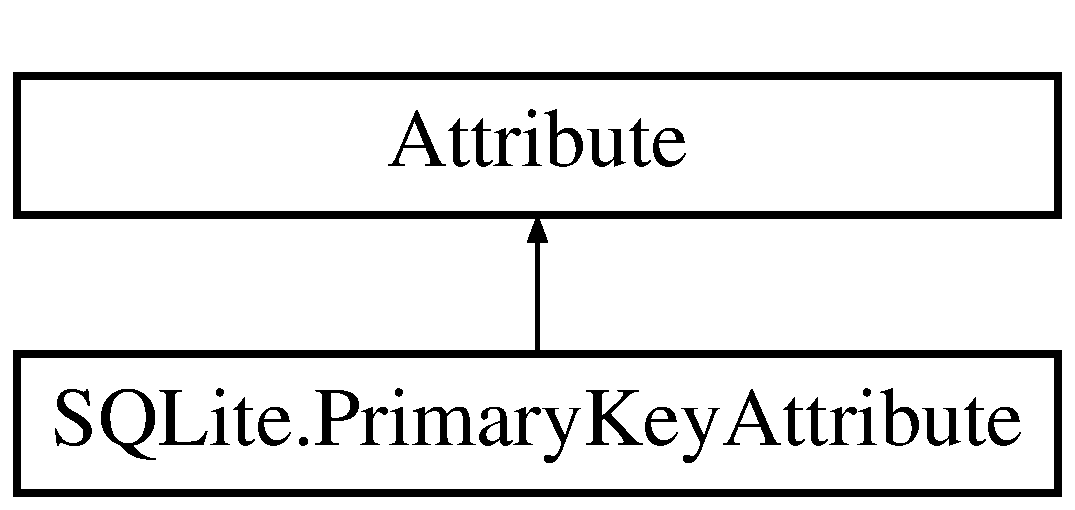
\includegraphics[height=2.000000cm]{classSQLite_1_1PrimaryKeyAttribute}
\end{center}
\end{figure}


The documentation for this class was generated from the following file\+:\begin{DoxyCompactItemize}
\item 
packages/sqlite-\/net.\+1.\+0.\+8/content/S\+Q\+Lite.\+cs\end{DoxyCompactItemize}

\hypertarget{classCore_1_1Models_1_1Region}{\section{Core.\-Models.\-Region Class Reference}
\label{classCore_1_1Models_1_1Region}\index{Core.\-Models.\-Region@{Core.\-Models.\-Region}}
}


A part of the world. Contains a \hyperlink{classCore_1_1Models_1_1RegionPosition}{Region\-Position} which determinates where (in the world) the region is. Also contains all entities to a specific time and all actions which were executed on the region.  


\subsection*{Classes}
\begin{DoxyCompactItemize}
\item 
class \hyperlink{classCore_1_1Models_1_1Region_1_1DatedActions}{Dated\-Actions}
\item 
class \hyperlink{classCore_1_1Models_1_1Region_1_1DatedEntities}{Dated\-Entities}
\end{DoxyCompactItemize}
\subsection*{Public Member Functions}
\begin{DoxyCompactItemize}
\item 
\hypertarget{classCore_1_1Models_1_1Region_a36ae96644a4ac7f34c2b608f56df38fc}{{\bfseries Region} (\hyperlink{classCore_1_1Models_1_1Region}{Region} region)}\label{classCore_1_1Models_1_1Region_a36ae96644a4ac7f34c2b608f56df38fc}

\item 
\hypertarget{classCore_1_1Models_1_1Region_a68736570a0df9f1e9b64d6a9d6744c02}{{\bfseries Region} (\hyperlink{classCore_1_1Models_1_1RegionPosition}{Region\-Position} region\-Position)}\label{classCore_1_1Models_1_1Region_a68736570a0df9f1e9b64d6a9d6744c02}

\item 
\hypertarget{classCore_1_1Models_1_1Region_afcf20af4ea09f9eed57e373a8a8210ea}{{\bfseries Region} (\hyperlink{classCore_1_1Models_1_1RegionPosition}{Region\-Position} region\-Position, \hyperlink{classCore_1_1Models_1_1Definitions_1_1TerrainDefinition}{Terrain\-Definition}\mbox{[},\mbox{]} terrains)}\label{classCore_1_1Models_1_1Region_afcf20af4ea09f9eed57e373a8a8210ea}

\item 
void \hyperlink{classCore_1_1Models_1_1Region_ad5e343aa96c3a1a28f5a98df87272cd9}{Add\-Terrain} (\hyperlink{classCore_1_1Models_1_1Definitions_1_1TerrainDefinition}{Terrain\-Definition}\mbox{[},\mbox{]} terrains)
\begin{DoxyCompactList}\small\item\em Adds the terrain afterward if the region was created without. \end{DoxyCompactList}\item 
\hyperlink{classCore_1_1Models_1_1Definitions_1_1TerrainDefinition}{Terrain\-Definition} \hyperlink{classCore_1_1Models_1_1Region_a1a49bf46e734963dc63aeb2cd2ce4063}{Get\-Terrain} (\hyperlink{classCore_1_1Models_1_1CellPosition}{Cell\-Position} cell\-Position)
\item 
\hyperlink{classCore_1_1Models_1_1Entity}{Entity} \hyperlink{classCore_1_1Models_1_1Region_aef86ef05f6bc2d535aca5d902e0c2731}{Get\-Entity} (\hyperlink{classCore_1_1Models_1_1CellPosition}{Cell\-Position} cell\-Position)
\begin{DoxyCompactList}\small\item\em Returns Buildings or Units at the given position \end{DoxyCompactList}\item 
void \hyperlink{classCore_1_1Models_1_1Region_ab696b3c1b6cc9d55b3c4eae768339ebd}{Add\-Entity} (Date\-Time date\-Time, \hyperlink{classCore_1_1Models_1_1Entity}{Entity} entity)
\begin{DoxyCompactList}\small\item\em Adds the entity to a specific time. \end{DoxyCompactList}\item 
void \hyperlink{classCore_1_1Models_1_1Region_a05d102bebab28be04e9184ed438b6cda}{Remove\-Entity} (Date\-Time date\-Time, \hyperlink{classCore_1_1Models_1_1Entity}{Entity} entity)
\begin{DoxyCompactList}\small\item\em Removes the entity to a specific time. \end{DoxyCompactList}\item 
\hypertarget{classCore_1_1Models_1_1Region_a4d5cf1050b208c1d06fcf344027dabf9}{\hyperlink{classCore_1_1Models_1_1Region_1_1DatedEntities}{Dated\-Entities} {\bfseries Get\-Entities} ()}\label{classCore_1_1Models_1_1Region_a4d5cf1050b208c1d06fcf344027dabf9}

\item 
\hyperlink{classCore_1_1Models_1_1Region_1_1DatedActions}{Dated\-Actions} \hyperlink{classCore_1_1Models_1_1Region_ab1e90f76e173a9a28396f806f274b697}{Get\-Completed\-Actions} (Date\-Time start\-Time)
\begin{DoxyCompactList}\small\item\em Builds a new list with all actions which are lower then the given start\-Time. \end{DoxyCompactList}\item 
\hypertarget{classCore_1_1Models_1_1Region_a44181d46f6b2541119734f74cd195365}{bool {\bfseries Lock\-Writer} ()}\label{classCore_1_1Models_1_1Region_a44181d46f6b2541119734f74cd195365}

\item 
\hypertarget{classCore_1_1Models_1_1Region_a377dbd594c64a01e00234efa9d91aa01}{void {\bfseries Release\-Writer} ()}\label{classCore_1_1Models_1_1Region_a377dbd594c64a01e00234efa9d91aa01}

\item 
\hypertarget{classCore_1_1Models_1_1Region_a33168014b3d76ef375e03fe123c6e172}{bool {\bfseries Lock\-Reader} ()}\label{classCore_1_1Models_1_1Region_a33168014b3d76ef375e03fe123c6e172}

\item 
\hypertarget{classCore_1_1Models_1_1Region_ab4fdcaab29033ad62ac611f74aeeab70}{void {\bfseries Release\-Reader} ()}\label{classCore_1_1Models_1_1Region_ab4fdcaab29033ad62ac611f74aeeab70}

\item 
void \hyperlink{classCore_1_1Models_1_1Region_a73612bd601b7c22498bb599e82e83cfb}{Add\-Completed\-Action} (\hyperlink{classCore_1_1Models_1_1Action}{Core.\-Models.\-Action} action)
\begin{DoxyCompactList}\small\item\em An \hyperlink{classCore_1_1Models_1_1Action}{Action} was executed and affected this region, then it should be added with Add\-Completed\-Action. \end{DoxyCompactList}\end{DoxyCompactItemize}
\subsection*{Properties}
\begin{DoxyCompactItemize}
\item 
bool \hyperlink{classCore_1_1Models_1_1Region_a8521c3cdb0ee6884d5e394217b44c66e}{Exist}\hspace{0.3cm}{\ttfamily  \mbox{[}get\mbox{]}}
\begin{DoxyCompactList}\small\item\em Gets a value indicating whether this base.\-model.\-Region really exist. Empty regions always return false. A region is empty if the terrain can't be loaded. (as example, bescause there were connection issues at the client -\/ or the region file don't exist) \end{DoxyCompactList}\item 
\hypertarget{classCore_1_1Models_1_1Region_a2b370559aea0f72e9c2ee19dfcc7f7d8}{\hyperlink{classCore_1_1Models_1_1RegionPosition}{Region\-Position} {\bfseries Region\-Position}\hspace{0.3cm}{\ttfamily  \mbox{[}get\mbox{]}}}\label{classCore_1_1Models_1_1Region_a2b370559aea0f72e9c2ee19dfcc7f7d8}

\end{DoxyCompactItemize}


\subsection{Detailed Description}
A part of the world. Contains a \hyperlink{classCore_1_1Models_1_1RegionPosition}{Region\-Position} which determinates where (in the world) the region is. Also contains all entities to a specific time and all actions which were executed on the region. 



\subsection{Member Function Documentation}
\hypertarget{classCore_1_1Models_1_1Region_a73612bd601b7c22498bb599e82e83cfb}{\index{Core\-::\-Models\-::\-Region@{Core\-::\-Models\-::\-Region}!Add\-Completed\-Action@{Add\-Completed\-Action}}
\index{Add\-Completed\-Action@{Add\-Completed\-Action}!Core::Models::Region@{Core\-::\-Models\-::\-Region}}
\subsubsection[{Add\-Completed\-Action}]{\setlength{\rightskip}{0pt plus 5cm}void Core.\-Models.\-Region.\-Add\-Completed\-Action (
\begin{DoxyParamCaption}
\item[{{\bf Core.\-Models.\-Action}}]{action}
\end{DoxyParamCaption}
)\hspace{0.3cm}{\ttfamily [inline]}}}\label{classCore_1_1Models_1_1Region_a73612bd601b7c22498bb599e82e83cfb}


An \hyperlink{classCore_1_1Models_1_1Action}{Action} was executed and affected this region, then it should be added with Add\-Completed\-Action. 


\begin{DoxyParams}{Parameters}
{\em action} & \hyperlink{classCore_1_1Models_1_1Action}{Action}.\\
\hline
\end{DoxyParams}
\hypertarget{classCore_1_1Models_1_1Region_ab696b3c1b6cc9d55b3c4eae768339ebd}{\index{Core\-::\-Models\-::\-Region@{Core\-::\-Models\-::\-Region}!Add\-Entity@{Add\-Entity}}
\index{Add\-Entity@{Add\-Entity}!Core::Models::Region@{Core\-::\-Models\-::\-Region}}
\subsubsection[{Add\-Entity}]{\setlength{\rightskip}{0pt plus 5cm}void Core.\-Models.\-Region.\-Add\-Entity (
\begin{DoxyParamCaption}
\item[{Date\-Time}]{date\-Time, }
\item[{{\bf Entity}}]{entity}
\end{DoxyParamCaption}
)\hspace{0.3cm}{\ttfamily [inline]}}}\label{classCore_1_1Models_1_1Region_ab696b3c1b6cc9d55b3c4eae768339ebd}


Adds the entity to a specific time. 


\begin{DoxyParams}{Parameters}
{\em date\-Time} & Date time when the action was called.\\
\hline
{\em entity} & \hyperlink{classCore_1_1Models_1_1Entity}{Entity}.\\
\hline
\end{DoxyParams}
\hypertarget{classCore_1_1Models_1_1Region_ad5e343aa96c3a1a28f5a98df87272cd9}{\index{Core\-::\-Models\-::\-Region@{Core\-::\-Models\-::\-Region}!Add\-Terrain@{Add\-Terrain}}
\index{Add\-Terrain@{Add\-Terrain}!Core::Models::Region@{Core\-::\-Models\-::\-Region}}
\subsubsection[{Add\-Terrain}]{\setlength{\rightskip}{0pt plus 5cm}void Core.\-Models.\-Region.\-Add\-Terrain (
\begin{DoxyParamCaption}
\item[{{\bf Terrain\-Definition}}]{terrains\mbox{[},\mbox{]}}
\end{DoxyParamCaption}
)\hspace{0.3cm}{\ttfamily [inline]}}}\label{classCore_1_1Models_1_1Region_ad5e343aa96c3a1a28f5a98df87272cd9}


Adds the terrain afterward if the region was created without. 


\begin{DoxyParams}{Parameters}
{\em terrains} & 2\-D array of Terrains\-Type \\
\hline
\end{DoxyParams}
\hypertarget{classCore_1_1Models_1_1Region_ab1e90f76e173a9a28396f806f274b697}{\index{Core\-::\-Models\-::\-Region@{Core\-::\-Models\-::\-Region}!Get\-Completed\-Actions@{Get\-Completed\-Actions}}
\index{Get\-Completed\-Actions@{Get\-Completed\-Actions}!Core::Models::Region@{Core\-::\-Models\-::\-Region}}
\subsubsection[{Get\-Completed\-Actions}]{\setlength{\rightskip}{0pt plus 5cm}{\bf Dated\-Actions} Core.\-Models.\-Region.\-Get\-Completed\-Actions (
\begin{DoxyParamCaption}
\item[{Date\-Time}]{start\-Time}
\end{DoxyParamCaption}
)\hspace{0.3cm}{\ttfamily [inline]}}}\label{classCore_1_1Models_1_1Region_ab1e90f76e173a9a28396f806f274b697}


Builds a new list with all actions which are lower then the given start\-Time. 


\begin{DoxyParams}{Parameters}
{\em start\-Time} & Datetime when region was lasttime loaded.\\
\hline
\end{DoxyParams}
\hypertarget{classCore_1_1Models_1_1Region_aef86ef05f6bc2d535aca5d902e0c2731}{\index{Core\-::\-Models\-::\-Region@{Core\-::\-Models\-::\-Region}!Get\-Entity@{Get\-Entity}}
\index{Get\-Entity@{Get\-Entity}!Core::Models::Region@{Core\-::\-Models\-::\-Region}}
\subsubsection[{Get\-Entity}]{\setlength{\rightskip}{0pt plus 5cm}{\bf Entity} Core.\-Models.\-Region.\-Get\-Entity (
\begin{DoxyParamCaption}
\item[{{\bf Cell\-Position}}]{cell\-Position}
\end{DoxyParamCaption}
)\hspace{0.3cm}{\ttfamily [inline]}}}\label{classCore_1_1Models_1_1Region_aef86ef05f6bc2d535aca5d902e0c2731}


Returns Buildings or Units at the given position 

\begin{DoxyReturn}{Returns}
The entity or null when there was no entity.
\end{DoxyReturn}

\begin{DoxyParams}{Parameters}
{\em cell\-Position} & Cell position.\\
\hline
\end{DoxyParams}
\hypertarget{classCore_1_1Models_1_1Region_a1a49bf46e734963dc63aeb2cd2ce4063}{\index{Core\-::\-Models\-::\-Region@{Core\-::\-Models\-::\-Region}!Get\-Terrain@{Get\-Terrain}}
\index{Get\-Terrain@{Get\-Terrain}!Core::Models::Region@{Core\-::\-Models\-::\-Region}}
\subsubsection[{Get\-Terrain}]{\setlength{\rightskip}{0pt plus 5cm}{\bf Terrain\-Definition} Core.\-Models.\-Region.\-Get\-Terrain (
\begin{DoxyParamCaption}
\item[{{\bf Cell\-Position}}]{cell\-Position}
\end{DoxyParamCaption}
)\hspace{0.3cm}{\ttfamily [inline]}}}\label{classCore_1_1Models_1_1Region_a1a49bf46e734963dc63aeb2cd2ce4063}




\begin{DoxyReturn}{Returns}
Returns the Terrain\-Defintion of the specific given cell\-Position.
\end{DoxyReturn}

\begin{DoxyParams}{Parameters}
{\em cell\-Position} & Cell position.\\
\hline
\end{DoxyParams}
\hypertarget{classCore_1_1Models_1_1Region_a05d102bebab28be04e9184ed438b6cda}{\index{Core\-::\-Models\-::\-Region@{Core\-::\-Models\-::\-Region}!Remove\-Entity@{Remove\-Entity}}
\index{Remove\-Entity@{Remove\-Entity}!Core::Models::Region@{Core\-::\-Models\-::\-Region}}
\subsubsection[{Remove\-Entity}]{\setlength{\rightskip}{0pt plus 5cm}void Core.\-Models.\-Region.\-Remove\-Entity (
\begin{DoxyParamCaption}
\item[{Date\-Time}]{date\-Time, }
\item[{{\bf Entity}}]{entity}
\end{DoxyParamCaption}
)\hspace{0.3cm}{\ttfamily [inline]}}}\label{classCore_1_1Models_1_1Region_a05d102bebab28be04e9184ed438b6cda}


Removes the entity to a specific time. 


\begin{DoxyParams}{Parameters}
{\em date\-Time} & Date time when the action was called.\\
\hline
{\em entity} & \hyperlink{classCore_1_1Models_1_1Entity}{Entity}.\\
\hline
\end{DoxyParams}


\subsection{Property Documentation}
\hypertarget{classCore_1_1Models_1_1Region_a8521c3cdb0ee6884d5e394217b44c66e}{\index{Core\-::\-Models\-::\-Region@{Core\-::\-Models\-::\-Region}!Exist@{Exist}}
\index{Exist@{Exist}!Core::Models::Region@{Core\-::\-Models\-::\-Region}}
\subsubsection[{Exist}]{\setlength{\rightskip}{0pt plus 5cm}bool Core.\-Models.\-Region.\-Exist\hspace{0.3cm}{\ttfamily [get]}}}\label{classCore_1_1Models_1_1Region_a8521c3cdb0ee6884d5e394217b44c66e}


Gets a value indicating whether this base.\-model.\-Region really exist. Empty regions always return false. A region is empty if the terrain can't be loaded. (as example, bescause there were connection issues at the client -\/ or the region file don't exist) 

{\ttfamily true} if exist; otherwise, {\ttfamily false}.

The documentation for this class was generated from the following file\-:\begin{DoxyCompactItemize}
\item 
base/\-Models/\-Map/Region.\-cs\end{DoxyCompactItemize}

\hypertarget{classServer_1_1Controllers_1_1APIController_1_1RegionData}{}\section{Server.\+Controllers.\+A\+P\+I\+Controller.\+Region\+Data Class Reference}
\label{classServer_1_1Controllers_1_1APIController_1_1RegionData}\index{Server.\+Controllers.\+A\+P\+I\+Controller.\+Region\+Data@{Server.\+Controllers.\+A\+P\+I\+Controller.\+Region\+Data}}


Region data.  


\subsection*{Public Attributes}
\begin{DoxyCompactItemize}
\item 
Linked\+List$<$ Linked\+List$<$ \hyperlink{classCore_1_1Models_1_1Entity}{Core.\+Models.\+Entity} $>$ $>$ \hyperlink{classServer_1_1Controllers_1_1APIController_1_1RegionData_a515c8be86ead173ab0e21c57a93cd174}{Entity\+Dict}
\begin{DoxyCompactList}\small\item\em The entities in every region. \end{DoxyCompactList}\item 
Linked\+List$<$ Linked\+List$<$ \hyperlink{classCore_1_1Models_1_1Action}{Core.\+Models.\+Action} $>$ $>$ \hyperlink{classServer_1_1Controllers_1_1APIController_1_1RegionData_a15b7109e6735a6e66ed251c195aaf937}{Action\+Dict}
\begin{DoxyCompactList}\small\item\em The actions in every region. \end{DoxyCompactList}\end{DoxyCompactItemize}


\subsection{Detailed Description}
Region data. 



\subsection{Member Data Documentation}
\hypertarget{classServer_1_1Controllers_1_1APIController_1_1RegionData_a15b7109e6735a6e66ed251c195aaf937}{}\index{Server\+::\+Controllers\+::\+A\+P\+I\+Controller\+::\+Region\+Data@{Server\+::\+Controllers\+::\+A\+P\+I\+Controller\+::\+Region\+Data}!Action\+Dict@{Action\+Dict}}
\index{Action\+Dict@{Action\+Dict}!Server\+::\+Controllers\+::\+A\+P\+I\+Controller\+::\+Region\+Data@{Server\+::\+Controllers\+::\+A\+P\+I\+Controller\+::\+Region\+Data}}
\subsubsection[{Action\+Dict}]{\setlength{\rightskip}{0pt plus 5cm}Linked\+List$<$Linked\+List$<${\bf Core.\+Models.\+Action}$>$ $>$ Server.\+Controllers.\+A\+P\+I\+Controller.\+Region\+Data.\+Action\+Dict}\label{classServer_1_1Controllers_1_1APIController_1_1RegionData_a15b7109e6735a6e66ed251c195aaf937}


The actions in every region. 

\hypertarget{classServer_1_1Controllers_1_1APIController_1_1RegionData_a515c8be86ead173ab0e21c57a93cd174}{}\index{Server\+::\+Controllers\+::\+A\+P\+I\+Controller\+::\+Region\+Data@{Server\+::\+Controllers\+::\+A\+P\+I\+Controller\+::\+Region\+Data}!Entity\+Dict@{Entity\+Dict}}
\index{Entity\+Dict@{Entity\+Dict}!Server\+::\+Controllers\+::\+A\+P\+I\+Controller\+::\+Region\+Data@{Server\+::\+Controllers\+::\+A\+P\+I\+Controller\+::\+Region\+Data}}
\subsubsection[{Entity\+Dict}]{\setlength{\rightskip}{0pt plus 5cm}Linked\+List$<$Linked\+List$<${\bf Core.\+Models.\+Entity}$>$ $>$ Server.\+Controllers.\+A\+P\+I\+Controller.\+Region\+Data.\+Entity\+Dict}\label{classServer_1_1Controllers_1_1APIController_1_1RegionData_a515c8be86ead173ab0e21c57a93cd174}


The entities in every region. 



The documentation for this class was generated from the following file\+:\begin{DoxyCompactItemize}
\item 
tcpserver/\+Controllers/A\+P\+I\+Controller.\+cs\end{DoxyCompactItemize}

\hypertarget{classCore_1_1Models_1_1RegionManager}{}\section{Core.\+Models.\+Region\+Manager Class Reference}
\label{classCore_1_1Models_1_1RegionManager}\index{Core.\+Models.\+Region\+Manager@{Core.\+Models.\+Region\+Manager}}


Contains all loaded Regions.  


\subsection*{Public Member Functions}
\begin{DoxyCompactItemize}
\item 
\hyperlink{classCore_1_1Models_1_1RegionManager_acfec42c6756010d6557616374f7cd37d}{Region\+Manager} ()
\begin{DoxyCompactList}\small\item\em Initializes a new instance of the \hyperlink{classCore_1_1Models_1_1RegionManager}{Core.\+Models.\+Region\+Manager} class. \end{DoxyCompactList}\item 
\hyperlink{classCore_1_1Models_1_1Region}{Region} \hyperlink{classCore_1_1Models_1_1RegionManager_a67a6954541a89c4135f414de61408ef8}{Get\+Region} (\hyperlink{classCore_1_1Models_1_1RegionPosition}{Region\+Position} region\+Position)
\begin{DoxyCompactList}\small\item\em Gets the region depending on the region position. \end{DoxyCompactList}\item 
void \hyperlink{classCore_1_1Models_1_1RegionManager_a2b44e4b56f8c00120f87f0b5bd0b1bcf}{Add\+Region} (\hyperlink{classCore_1_1Models_1_1Region}{Region} region)
\begin{DoxyCompactList}\small\item\em Adds an region. \end{DoxyCompactList}\end{DoxyCompactItemize}
\subsection*{Public Attributes}
\begin{DoxyCompactItemize}
\item 
Concurrent\+Dictionary$<$ \hyperlink{classCore_1_1Models_1_1RegionPosition}{Region\+Position}, \hyperlink{classCore_1_1Models_1_1Region}{Region} $>$ \hyperlink{classCore_1_1Models_1_1RegionManager_a0c119456a8a49f28a14213dad448a5da}{Regions}
\begin{DoxyCompactList}\small\item\em The regions. \end{DoxyCompactList}\end{DoxyCompactItemize}


\subsection{Detailed Description}
Contains all loaded Regions. 



\subsection{Constructor \& Destructor Documentation}
\hypertarget{classCore_1_1Models_1_1RegionManager_acfec42c6756010d6557616374f7cd37d}{}\index{Core\+::\+Models\+::\+Region\+Manager@{Core\+::\+Models\+::\+Region\+Manager}!Region\+Manager@{Region\+Manager}}
\index{Region\+Manager@{Region\+Manager}!Core\+::\+Models\+::\+Region\+Manager@{Core\+::\+Models\+::\+Region\+Manager}}
\subsubsection[{Region\+Manager()}]{\setlength{\rightskip}{0pt plus 5cm}Core.\+Models.\+Region\+Manager.\+Region\+Manager (
\begin{DoxyParamCaption}
{}
\end{DoxyParamCaption}
)}\label{classCore_1_1Models_1_1RegionManager_acfec42c6756010d6557616374f7cd37d}


Initializes a new instance of the \hyperlink{classCore_1_1Models_1_1RegionManager}{Core.\+Models.\+Region\+Manager} class. 



\subsection{Member Function Documentation}
\hypertarget{classCore_1_1Models_1_1RegionManager_a2b44e4b56f8c00120f87f0b5bd0b1bcf}{}\index{Core\+::\+Models\+::\+Region\+Manager@{Core\+::\+Models\+::\+Region\+Manager}!Add\+Region@{Add\+Region}}
\index{Add\+Region@{Add\+Region}!Core\+::\+Models\+::\+Region\+Manager@{Core\+::\+Models\+::\+Region\+Manager}}
\subsubsection[{Add\+Region(\+Region region)}]{\setlength{\rightskip}{0pt plus 5cm}void Core.\+Models.\+Region\+Manager.\+Add\+Region (
\begin{DoxyParamCaption}
\item[{{\bf Region}}]{region}
\end{DoxyParamCaption}
)}\label{classCore_1_1Models_1_1RegionManager_a2b44e4b56f8c00120f87f0b5bd0b1bcf}


Adds an region. 


\begin{DoxyParams}{Parameters}
{\em region} & \hyperlink{classCore_1_1Models_1_1Region}{Region} which should be added.\\
\hline
\end{DoxyParams}
\hypertarget{classCore_1_1Models_1_1RegionManager_a67a6954541a89c4135f414de61408ef8}{}\index{Core\+::\+Models\+::\+Region\+Manager@{Core\+::\+Models\+::\+Region\+Manager}!Get\+Region@{Get\+Region}}
\index{Get\+Region@{Get\+Region}!Core\+::\+Models\+::\+Region\+Manager@{Core\+::\+Models\+::\+Region\+Manager}}
\subsubsection[{Get\+Region(\+Region\+Position region\+Position)}]{\setlength{\rightskip}{0pt plus 5cm}{\bf Region} Core.\+Models.\+Region\+Manager.\+Get\+Region (
\begin{DoxyParamCaption}
\item[{{\bf Region\+Position}}]{region\+Position}
\end{DoxyParamCaption}
)}\label{classCore_1_1Models_1_1RegionManager_a67a6954541a89c4135f414de61408ef8}


Gets the region depending on the region position. 

\begin{DoxyReturn}{Returns}
The region.
\end{DoxyReturn}

\begin{DoxyParams}{Parameters}
{\em region\+Position} & \hyperlink{classCore_1_1Models_1_1Region}{Region} position.\\
\hline
\end{DoxyParams}


\subsection{Member Data Documentation}
\hypertarget{classCore_1_1Models_1_1RegionManager_a0c119456a8a49f28a14213dad448a5da}{}\index{Core\+::\+Models\+::\+Region\+Manager@{Core\+::\+Models\+::\+Region\+Manager}!Regions@{Regions}}
\index{Regions@{Regions}!Core\+::\+Models\+::\+Region\+Manager@{Core\+::\+Models\+::\+Region\+Manager}}
\subsubsection[{Regions}]{\setlength{\rightskip}{0pt plus 5cm}Concurrent\+Dictionary$<${\bf Region\+Position}, {\bf Region}$>$ Core.\+Models.\+Region\+Manager.\+Regions}\label{classCore_1_1Models_1_1RegionManager_a0c119456a8a49f28a14213dad448a5da}


The regions. 



The documentation for this class was generated from the following file\+:\begin{DoxyCompactItemize}
\item 
base/\+Models/\+Manager/Region\+Manager.\+cs\end{DoxyCompactItemize}

\hypertarget{classClient_1_1Common_1_1Manager_1_1RegionManagerController}{}\section{Client.\+Common.\+Manager.\+Region\+Manager\+Controller Class Reference}
\label{classClient_1_1Common_1_1Manager_1_1RegionManagerController}\index{Client.\+Common.\+Manager.\+Region\+Manager\+Controller@{Client.\+Common.\+Manager.\+Region\+Manager\+Controller}}


The Region manager controller to control the regions.  


Inheritance diagram for Client.\+Common.\+Manager.\+Region\+Manager\+Controller\+:\begin{figure}[H]
\begin{center}
\leavevmode
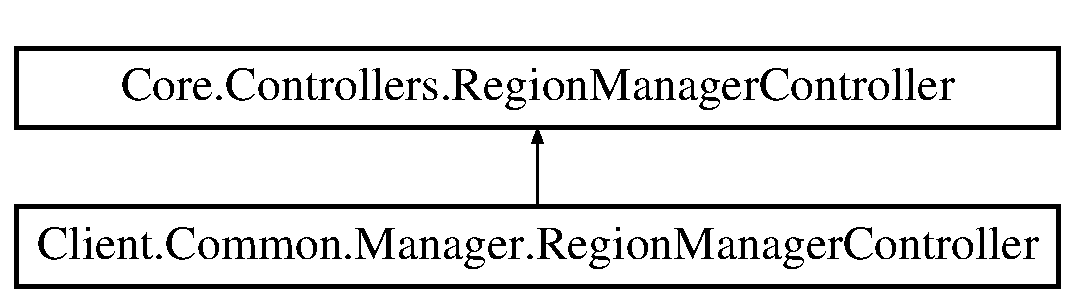
\includegraphics[height=2.000000cm]{classClient_1_1Common_1_1Manager_1_1RegionManagerController}
\end{center}
\end{figure}
\subsection*{Public Member Functions}
\begin{DoxyCompactItemize}
\item 
\hyperlink{classClient_1_1Common_1_1Manager_1_1RegionManagerController_a89a6a0097ec0ed4b2e26c2dcf312a27d}{Region\+Manager\+Controller} ()
\begin{DoxyCompactList}\small\item\em Initializes a new instance of the \hyperlink{classClient_1_1Common_1_1Manager_1_1RegionManagerController}{Client.\+Common.\+Manager.\+Region\+Manager\+Controller} class. \end{DoxyCompactList}\item 
\hyperlink{classCore_1_1Models_1_1Region}{Region} \hyperlink{classClient_1_1Common_1_1Manager_1_1RegionManagerController_aec46cc3e22d4ebc001c4e19fc0c0cf48}{Get\+Region\+By\+Geolocator} ()
\begin{DoxyCompactList}\small\item\em Gets the region by current geo location. \end{DoxyCompactList}\item 
\hyperlink{classCore_1_1Models_1_1Region}{Region} \hyperlink{classClient_1_1Common_1_1Manager_1_1RegionManagerController_a449853590dde1fc7fc56388afafd6bf3}{Get\+Region\+By\+Game\+Position} (\hyperlink{classCore_1_1Models_1_1Position}{Position} game\+World\+Position)
\begin{DoxyCompactList}\small\item\em Gets the region by game position. \end{DoxyCompactList}\item 
override \hyperlink{classCore_1_1Models_1_1Region}{Region} \hyperlink{classClient_1_1Common_1_1Manager_1_1RegionManagerController_a63a3b272d688663f463c29d212cdf2e9}{Get\+Region} (\hyperlink{classCore_1_1Models_1_1RegionPosition}{Region\+Position} region\+Position)
\begin{DoxyCompactList}\small\item\em Gets the region.\+If needed loads the region. \end{DoxyCompactList}\item 
async Task$<$ bool $>$ \hyperlink{classClient_1_1Common_1_1Manager_1_1RegionManagerController_a4e248f5877d9aa7b944cff4084ffdc67}{Do\+Action\+Async} (\hyperlink{classCore_1_1Models_1_1Position}{Core.\+Models.\+Position} current\+Game\+Position, \hyperlink{classCore_1_1Models_1_1Action}{Core.\+Models.\+Action}\mbox{[}$\,$\mbox{]} actions)
\begin{DoxyCompactList}\small\item\em Dos the action async. Send the actions to the server and load the response. \end{DoxyCompactList}\item 
Hash\+Set$<$ \hyperlink{classCore_1_1Models_1_1RegionPosition}{Region\+Position} $>$ \hyperlink{classClient_1_1Common_1_1Manager_1_1RegionManagerController_a200816e068a646522d5ecb069c637698}{Get\+World\+Near\+Region\+Positions} (\hyperlink{classCore_1_1Models_1_1RegionPosition}{Region\+Position} region\+Position)
\begin{DoxyCompactList}\small\item\em Gets the world near the region position. Around 5x5 regions at the region position. \end{DoxyCompactList}\item 
async Task \hyperlink{classClient_1_1Common_1_1Manager_1_1RegionManagerController_a754eab991e880017a9e21b03ee220d25}{Load\+Terrain\+Async} (\hyperlink{classCore_1_1Models_1_1Region}{Region} region)
\begin{DoxyCompactList}\small\item\em Loads the terrain async over the network controller and adds the region to the world. \end{DoxyCompactList}\end{DoxyCompactItemize}
\subsection*{Additional Inherited Members}


\subsection{Detailed Description}
The Region manager controller to control the regions. 



\subsection{Constructor \& Destructor Documentation}
\hypertarget{classClient_1_1Common_1_1Manager_1_1RegionManagerController_a89a6a0097ec0ed4b2e26c2dcf312a27d}{}\index{Client\+::\+Common\+::\+Manager\+::\+Region\+Manager\+Controller@{Client\+::\+Common\+::\+Manager\+::\+Region\+Manager\+Controller}!Region\+Manager\+Controller@{Region\+Manager\+Controller}}
\index{Region\+Manager\+Controller@{Region\+Manager\+Controller}!Client\+::\+Common\+::\+Manager\+::\+Region\+Manager\+Controller@{Client\+::\+Common\+::\+Manager\+::\+Region\+Manager\+Controller}}
\subsubsection[{Region\+Manager\+Controller()}]{\setlength{\rightskip}{0pt plus 5cm}Client.\+Common.\+Manager.\+Region\+Manager\+Controller.\+Region\+Manager\+Controller (
\begin{DoxyParamCaption}
{}
\end{DoxyParamCaption}
)}\label{classClient_1_1Common_1_1Manager_1_1RegionManagerController_a89a6a0097ec0ed4b2e26c2dcf312a27d}


Initializes a new instance of the \hyperlink{classClient_1_1Common_1_1Manager_1_1RegionManagerController}{Client.\+Common.\+Manager.\+Region\+Manager\+Controller} class. 



\subsection{Member Function Documentation}
\hypertarget{classClient_1_1Common_1_1Manager_1_1RegionManagerController_a4e248f5877d9aa7b944cff4084ffdc67}{}\index{Client\+::\+Common\+::\+Manager\+::\+Region\+Manager\+Controller@{Client\+::\+Common\+::\+Manager\+::\+Region\+Manager\+Controller}!Do\+Action\+Async@{Do\+Action\+Async}}
\index{Do\+Action\+Async@{Do\+Action\+Async}!Client\+::\+Common\+::\+Manager\+::\+Region\+Manager\+Controller@{Client\+::\+Common\+::\+Manager\+::\+Region\+Manager\+Controller}}
\subsubsection[{Do\+Action\+Async(\+Core.\+Models.\+Position current\+Game\+Position, Core.\+Models.\+Action[] actions)}]{\setlength{\rightskip}{0pt plus 5cm}async Task$<$bool$>$ Client.\+Common.\+Manager.\+Region\+Manager\+Controller.\+Do\+Action\+Async (
\begin{DoxyParamCaption}
\item[{{\bf Core.\+Models.\+Position}}]{current\+Game\+Position, }
\item[{{\bf Core.\+Models.\+Action}\mbox{[}$\,$\mbox{]}}]{actions}
\end{DoxyParamCaption}
)}\label{classClient_1_1Common_1_1Manager_1_1RegionManagerController_a4e248f5877d9aa7b944cff4084ffdc67}


Dos the action async. Send the actions to the server and load the response. 

\begin{DoxyReturn}{Returns}
True once the action is done.
\end{DoxyReturn}

\begin{DoxyParams}{Parameters}
{\em current\+Game\+Position} & Current game position.\\
\hline
{\em actions} & Actions which should be executed.\\
\hline
\end{DoxyParams}
\hypertarget{classClient_1_1Common_1_1Manager_1_1RegionManagerController_a63a3b272d688663f463c29d212cdf2e9}{}\index{Client\+::\+Common\+::\+Manager\+::\+Region\+Manager\+Controller@{Client\+::\+Common\+::\+Manager\+::\+Region\+Manager\+Controller}!Get\+Region@{Get\+Region}}
\index{Get\+Region@{Get\+Region}!Client\+::\+Common\+::\+Manager\+::\+Region\+Manager\+Controller@{Client\+::\+Common\+::\+Manager\+::\+Region\+Manager\+Controller}}
\subsubsection[{Get\+Region(\+Region\+Position region\+Position)}]{\setlength{\rightskip}{0pt plus 5cm}override {\bf Region} Client.\+Common.\+Manager.\+Region\+Manager\+Controller.\+Get\+Region (
\begin{DoxyParamCaption}
\item[{{\bf Region\+Position}}]{region\+Position}
\end{DoxyParamCaption}
)\hspace{0.3cm}{\ttfamily [virtual]}}\label{classClient_1_1Common_1_1Manager_1_1RegionManagerController_a63a3b272d688663f463c29d212cdf2e9}


Gets the region.\+If needed loads the region. 

\begin{DoxyReturn}{Returns}
The region.
\end{DoxyReturn}

\begin{DoxyParams}{Parameters}
{\em region\+Position} & Region position.\\
\hline
\end{DoxyParams}


Reimplemented from \hyperlink{classCore_1_1Controllers_1_1RegionManagerController_a1ce55cf6fb0ba5f0b5711e70ffb86467}{Core.\+Controllers.\+Region\+Manager\+Controller}.

\hypertarget{classClient_1_1Common_1_1Manager_1_1RegionManagerController_a449853590dde1fc7fc56388afafd6bf3}{}\index{Client\+::\+Common\+::\+Manager\+::\+Region\+Manager\+Controller@{Client\+::\+Common\+::\+Manager\+::\+Region\+Manager\+Controller}!Get\+Region\+By\+Game\+Position@{Get\+Region\+By\+Game\+Position}}
\index{Get\+Region\+By\+Game\+Position@{Get\+Region\+By\+Game\+Position}!Client\+::\+Common\+::\+Manager\+::\+Region\+Manager\+Controller@{Client\+::\+Common\+::\+Manager\+::\+Region\+Manager\+Controller}}
\subsubsection[{Get\+Region\+By\+Game\+Position(\+Position game\+World\+Position)}]{\setlength{\rightskip}{0pt plus 5cm}{\bf Region} Client.\+Common.\+Manager.\+Region\+Manager\+Controller.\+Get\+Region\+By\+Game\+Position (
\begin{DoxyParamCaption}
\item[{{\bf Position}}]{game\+World\+Position}
\end{DoxyParamCaption}
)}\label{classClient_1_1Common_1_1Manager_1_1RegionManagerController_a449853590dde1fc7fc56388afafd6bf3}


Gets the region by game position. 

\begin{DoxyReturn}{Returns}
The region by game position.
\end{DoxyReturn}

\begin{DoxyParams}{Parameters}
{\em game\+World\+Position} & Game world position.\\
\hline
\end{DoxyParams}
\hypertarget{classClient_1_1Common_1_1Manager_1_1RegionManagerController_aec46cc3e22d4ebc001c4e19fc0c0cf48}{}\index{Client\+::\+Common\+::\+Manager\+::\+Region\+Manager\+Controller@{Client\+::\+Common\+::\+Manager\+::\+Region\+Manager\+Controller}!Get\+Region\+By\+Geolocator@{Get\+Region\+By\+Geolocator}}
\index{Get\+Region\+By\+Geolocator@{Get\+Region\+By\+Geolocator}!Client\+::\+Common\+::\+Manager\+::\+Region\+Manager\+Controller@{Client\+::\+Common\+::\+Manager\+::\+Region\+Manager\+Controller}}
\subsubsection[{Get\+Region\+By\+Geolocator()}]{\setlength{\rightskip}{0pt plus 5cm}{\bf Region} Client.\+Common.\+Manager.\+Region\+Manager\+Controller.\+Get\+Region\+By\+Geolocator (
\begin{DoxyParamCaption}
{}
\end{DoxyParamCaption}
)}\label{classClient_1_1Common_1_1Manager_1_1RegionManagerController_aec46cc3e22d4ebc001c4e19fc0c0cf48}


Gets the region by current geo location. 

\begin{DoxyReturn}{Returns}
The region by current geo location.
\end{DoxyReturn}
\hypertarget{classClient_1_1Common_1_1Manager_1_1RegionManagerController_a200816e068a646522d5ecb069c637698}{}\index{Client\+::\+Common\+::\+Manager\+::\+Region\+Manager\+Controller@{Client\+::\+Common\+::\+Manager\+::\+Region\+Manager\+Controller}!Get\+World\+Near\+Region\+Positions@{Get\+World\+Near\+Region\+Positions}}
\index{Get\+World\+Near\+Region\+Positions@{Get\+World\+Near\+Region\+Positions}!Client\+::\+Common\+::\+Manager\+::\+Region\+Manager\+Controller@{Client\+::\+Common\+::\+Manager\+::\+Region\+Manager\+Controller}}
\subsubsection[{Get\+World\+Near\+Region\+Positions(\+Region\+Position region\+Position)}]{\setlength{\rightskip}{0pt plus 5cm}Hash\+Set$<${\bf Region\+Position}$>$ Client.\+Common.\+Manager.\+Region\+Manager\+Controller.\+Get\+World\+Near\+Region\+Positions (
\begin{DoxyParamCaption}
\item[{{\bf Region\+Position}}]{region\+Position}
\end{DoxyParamCaption}
)}\label{classClient_1_1Common_1_1Manager_1_1RegionManagerController_a200816e068a646522d5ecb069c637698}


Gets the world near the region position. Around 5x5 regions at the region position. 

\begin{DoxyReturn}{Returns}
The regions around the positions.
\end{DoxyReturn}

\begin{DoxyParams}{Parameters}
{\em region\+Position} & Region position.\\
\hline
\end{DoxyParams}
\hypertarget{classClient_1_1Common_1_1Manager_1_1RegionManagerController_a754eab991e880017a9e21b03ee220d25}{}\index{Client\+::\+Common\+::\+Manager\+::\+Region\+Manager\+Controller@{Client\+::\+Common\+::\+Manager\+::\+Region\+Manager\+Controller}!Load\+Terrain\+Async@{Load\+Terrain\+Async}}
\index{Load\+Terrain\+Async@{Load\+Terrain\+Async}!Client\+::\+Common\+::\+Manager\+::\+Region\+Manager\+Controller@{Client\+::\+Common\+::\+Manager\+::\+Region\+Manager\+Controller}}
\subsubsection[{Load\+Terrain\+Async(\+Region region)}]{\setlength{\rightskip}{0pt plus 5cm}async Task Client.\+Common.\+Manager.\+Region\+Manager\+Controller.\+Load\+Terrain\+Async (
\begin{DoxyParamCaption}
\item[{{\bf Region}}]{region}
\end{DoxyParamCaption}
)}\label{classClient_1_1Common_1_1Manager_1_1RegionManagerController_a754eab991e880017a9e21b03ee220d25}


Loads the terrain async over the network controller and adds the region to the world. 

\begin{DoxyReturn}{Returns}
The function as task.
\end{DoxyReturn}

\begin{DoxyParams}{Parameters}
{\em region} & Region which should be loaded.\\
\hline
\end{DoxyParams}


The documentation for this class was generated from the following file\+:\begin{DoxyCompactItemize}
\item 
client/client/client.\+Common/\+Manager/Region\+Manager\+Controller.\+cs\end{DoxyCompactItemize}

\hypertarget{classServer_1_1Controllers_1_1RegionManagerController}{\section{Server.\-Controllers.\-Region\-Manager\-Controller Class Reference}
\label{classServer_1_1Controllers_1_1RegionManagerController}\index{Server.\-Controllers.\-Region\-Manager\-Controller@{Server.\-Controllers.\-Region\-Manager\-Controller}}
}


Contains all loaded regions and loads regions.  


Inheritance diagram for Server.\-Controllers.\-Region\-Manager\-Controller\-:\begin{figure}[H]
\begin{center}
\leavevmode
\includegraphics[height=2.000000cm]{classServer_1_1Controllers_1_1RegionManagerController}
\end{center}
\end{figure}
\subsection*{Public Member Functions}
\begin{DoxyCompactItemize}
\item 
override \hyperlink{classCore_1_1Models_1_1Region}{Region} \hyperlink{classServer_1_1Controllers_1_1RegionManagerController_a14319718114aedea38984b1bf61395a4}{Get\-Region} (\hyperlink{classCore_1_1Models_1_1RegionPosition}{Region\-Position} region\-Position)
\begin{DoxyCompactList}\small\item\em Tries to get the Region. \end{DoxyCompactList}\end{DoxyCompactItemize}


\subsection{Detailed Description}
Contains all loaded regions and loads regions. 



\subsection{Member Function Documentation}
\hypertarget{classServer_1_1Controllers_1_1RegionManagerController_a14319718114aedea38984b1bf61395a4}{\index{Server\-::\-Controllers\-::\-Region\-Manager\-Controller@{Server\-::\-Controllers\-::\-Region\-Manager\-Controller}!Get\-Region@{Get\-Region}}
\index{Get\-Region@{Get\-Region}!Server::Controllers::RegionManagerController@{Server\-::\-Controllers\-::\-Region\-Manager\-Controller}}
\subsubsection[{Get\-Region}]{\setlength{\rightskip}{0pt plus 5cm}override {\bf Region} Server.\-Controllers.\-Region\-Manager\-Controller.\-Get\-Region (
\begin{DoxyParamCaption}
\item[{{\bf Region\-Position}}]{region\-Position}
\end{DoxyParamCaption}
)\hspace{0.3cm}{\ttfamily [inline]}, {\ttfamily [virtual]}}}\label{classServer_1_1Controllers_1_1RegionManagerController_a14319718114aedea38984b1bf61395a4}


Tries to get the Region. 

\begin{DoxyReturn}{Returns}
The region. If it couln't be loaded, region.\-exist is false.
\end{DoxyReturn}

\begin{DoxyParams}{Parameters}
{\em region\-Position} & Region position.\\
\hline
\end{DoxyParams}


Reimplemented from \hyperlink{classCore_1_1Controllers_1_1RegionManagerController}{Core.\-Controllers.\-Region\-Manager\-Controller}.



The documentation for this class was generated from the following file\-:\begin{DoxyCompactItemize}
\item 
server/\-Controllers/Region\-Manager\-Controller.\-cs\end{DoxyCompactItemize}

\hypertarget{classCore_1_1Controllers_1_1RegionManagerController}{}\section{Core.\+Controllers.\+Region\+Manager\+Controller Class Reference}
\label{classCore_1_1Controllers_1_1RegionManagerController}\index{Core.\+Controllers.\+Region\+Manager\+Controller@{Core.\+Controllers.\+Region\+Manager\+Controller}}


Loads and adds regions to the region manager  


Inheritance diagram for Core.\+Controllers.\+Region\+Manager\+Controller\+:\begin{figure}[H]
\begin{center}
\leavevmode
\includegraphics[height=1.812298cm]{classCore_1_1Controllers_1_1RegionManagerController}
\end{center}
\end{figure}
\subsection*{Public Member Functions}
\begin{DoxyCompactItemize}
\item 
\hyperlink{classCore_1_1Controllers_1_1RegionManagerController_aeea73e7911e9a19ff686d12db8f65a9c}{Region\+Manager\+Controller} ()
\begin{DoxyCompactList}\small\item\em Initializes a new instance of the \hyperlink{classCore_1_1Controllers_1_1RegionManagerController}{Core.\+Controllers.\+Region\+Manager\+Controller} class. \end{DoxyCompactList}\item 
virtual \hyperlink{classCore_1_1Models_1_1Region}{Region} \hyperlink{classCore_1_1Controllers_1_1RegionManagerController_a1ce55cf6fb0ba5f0b5711e70ffb86467}{Get\+Region} (\hyperlink{classCore_1_1Models_1_1RegionPosition}{Region\+Position} region\+Position)
\begin{DoxyCompactList}\small\item\em Gets the region. \end{DoxyCompactList}\end{DoxyCompactItemize}
\subsection*{Properties}
\begin{DoxyCompactItemize}
\item 
\hyperlink{classCore_1_1Models_1_1RegionManager}{Region\+Manager} \hyperlink{classCore_1_1Controllers_1_1RegionManagerController_a083ddefab3d734121ca256919bffa097}{Region\+Manager}\hspace{0.3cm}{\ttfamily  \mbox{[}get\mbox{]}}
\begin{DoxyCompactList}\small\item\em Gets the region manager. \end{DoxyCompactList}\end{DoxyCompactItemize}


\subsection{Detailed Description}
Loads and adds regions to the region manager 



\subsection{Constructor \& Destructor Documentation}
\hypertarget{classCore_1_1Controllers_1_1RegionManagerController_aeea73e7911e9a19ff686d12db8f65a9c}{}\index{Core\+::\+Controllers\+::\+Region\+Manager\+Controller@{Core\+::\+Controllers\+::\+Region\+Manager\+Controller}!Region\+Manager\+Controller@{Region\+Manager\+Controller}}
\index{Region\+Manager\+Controller@{Region\+Manager\+Controller}!Core\+::\+Controllers\+::\+Region\+Manager\+Controller@{Core\+::\+Controllers\+::\+Region\+Manager\+Controller}}
\subsubsection[{Region\+Manager\+Controller()}]{\setlength{\rightskip}{0pt plus 5cm}Core.\+Controllers.\+Region\+Manager\+Controller.\+Region\+Manager\+Controller (
\begin{DoxyParamCaption}
{}
\end{DoxyParamCaption}
)}\label{classCore_1_1Controllers_1_1RegionManagerController_aeea73e7911e9a19ff686d12db8f65a9c}


Initializes a new instance of the \hyperlink{classCore_1_1Controllers_1_1RegionManagerController}{Core.\+Controllers.\+Region\+Manager\+Controller} class. 



\subsection{Member Function Documentation}
\hypertarget{classCore_1_1Controllers_1_1RegionManagerController_a1ce55cf6fb0ba5f0b5711e70ffb86467}{}\index{Core\+::\+Controllers\+::\+Region\+Manager\+Controller@{Core\+::\+Controllers\+::\+Region\+Manager\+Controller}!Get\+Region@{Get\+Region}}
\index{Get\+Region@{Get\+Region}!Core\+::\+Controllers\+::\+Region\+Manager\+Controller@{Core\+::\+Controllers\+::\+Region\+Manager\+Controller}}
\subsubsection[{Get\+Region(\+Region\+Position region\+Position)}]{\setlength{\rightskip}{0pt plus 5cm}virtual {\bf Region} Core.\+Controllers.\+Region\+Manager\+Controller.\+Get\+Region (
\begin{DoxyParamCaption}
\item[{{\bf Region\+Position}}]{region\+Position}
\end{DoxyParamCaption}
)\hspace{0.3cm}{\ttfamily [virtual]}}\label{classCore_1_1Controllers_1_1RegionManagerController_a1ce55cf6fb0ba5f0b5711e70ffb86467}


Gets the region. 

\begin{DoxyReturn}{Returns}
The region.
\end{DoxyReturn}

\begin{DoxyParams}{Parameters}
{\em region\+Position} & Region position.\\
\hline
\end{DoxyParams}


Reimplemented in \hyperlink{classClient_1_1Common_1_1Manager_1_1RegionManagerController_a63a3b272d688663f463c29d212cdf2e9}{Client.\+Common.\+Manager.\+Region\+Manager\+Controller}, and \hyperlink{classServer_1_1Controllers_1_1RegionManagerController_a14319718114aedea38984b1bf61395a4}{Server.\+Controllers.\+Region\+Manager\+Controller}.



\subsection{Property Documentation}
\hypertarget{classCore_1_1Controllers_1_1RegionManagerController_a083ddefab3d734121ca256919bffa097}{}\index{Core\+::\+Controllers\+::\+Region\+Manager\+Controller@{Core\+::\+Controllers\+::\+Region\+Manager\+Controller}!Region\+Manager@{Region\+Manager}}
\index{Region\+Manager@{Region\+Manager}!Core\+::\+Controllers\+::\+Region\+Manager\+Controller@{Core\+::\+Controllers\+::\+Region\+Manager\+Controller}}
\subsubsection[{Region\+Manager}]{\setlength{\rightskip}{0pt plus 5cm}{\bf Region\+Manager} Core.\+Controllers.\+Region\+Manager\+Controller.\+Region\+Manager\hspace{0.3cm}{\ttfamily [get]}}\label{classCore_1_1Controllers_1_1RegionManagerController_a083ddefab3d734121ca256919bffa097}


Gets the region manager. 

The region manager.

The documentation for this class was generated from the following file\+:\begin{DoxyCompactItemize}
\item 
base/\+Controllers/Region\+Manager\+Controller.\+cs\end{DoxyCompactItemize}

\hypertarget{classCore_1_1Models_1_1RegionPosition}{\section{Core.\-Models.\-Region\-Position Class Reference}
\label{classCore_1_1Models_1_1RegionPosition}\index{Core.\-Models.\-Region\-Position@{Core.\-Models.\-Region\-Position}}
}


Represents a position of a region.  


Inheritance diagram for Core.\-Models.\-Region\-Position\-:\begin{figure}[H]
\begin{center}
\leavevmode
\includegraphics[height=2.000000cm]{classCore_1_1Models_1_1RegionPosition}
\end{center}
\end{figure}
\subsection*{Public Member Functions}
\begin{DoxyCompactItemize}
\item 
\hypertarget{classCore_1_1Models_1_1RegionPosition_ae02aba3016ef1e1eca5b3283bbd6068b}{{\bfseries Region\-Position} (int region\-X, int region\-Y)}\label{classCore_1_1Models_1_1RegionPosition_ae02aba3016ef1e1eca5b3283bbd6068b}

\item 
\hypertarget{classCore_1_1Models_1_1RegionPosition_a79f52954eeec48c9a5b06fd0a6ec9053}{{\bfseries Region\-Position} (\hyperlink{classCore_1_1Models_1_1Position}{Position} position)}\label{classCore_1_1Models_1_1RegionPosition_a79f52954eeec48c9a5b06fd0a6ec9053}

\item 
\hypertarget{classCore_1_1Models_1_1RegionPosition_a09edc96dddc599eedf2980effb36956a}{{\bfseries Region\-Position} (\hyperlink{classCore_1_1Models_1_1PositionI}{Position\-I} position)}\label{classCore_1_1Models_1_1RegionPosition_a09edc96dddc599eedf2980effb36956a}

\item 
\hypertarget{classCore_1_1Models_1_1RegionPosition_a120da8d2e0832f8a3c3b12f4e610d10c}{{\bfseries Region\-Position} (J\-Container obj)}\label{classCore_1_1Models_1_1RegionPosition_a120da8d2e0832f8a3c3b12f4e610d10c}

\item 
\hypertarget{classCore_1_1Models_1_1RegionPosition_a103e5d6c1fd5bc4ded06d98fb308bc63}{override bool {\bfseries Equals} (Object obj)}\label{classCore_1_1Models_1_1RegionPosition_a103e5d6c1fd5bc4ded06d98fb308bc63}

\item 
\hypertarget{classCore_1_1Models_1_1RegionPosition_ac39a779696243b79152ebde4f3029738}{override int {\bfseries Get\-Hash\-Code} ()}\label{classCore_1_1Models_1_1RegionPosition_ac39a779696243b79152ebde4f3029738}

\end{DoxyCompactItemize}
\subsection*{Static Public Member Functions}
\begin{DoxyCompactItemize}
\item 
\hypertarget{classCore_1_1Models_1_1RegionPosition_aab54c93c6d1a98929101e97539d3a0f7}{static \hyperlink{classCore_1_1Models_1_1RegionPosition}{Region\-Position} {\bfseries operator+} (\hyperlink{classCore_1_1Models_1_1RegionPosition}{Region\-Position} first, \hyperlink{classCore_1_1Models_1_1RegionPosition}{Region\-Position} second)}\label{classCore_1_1Models_1_1RegionPosition_aab54c93c6d1a98929101e97539d3a0f7}

\end{DoxyCompactItemize}
\subsection*{Properties}
\begin{DoxyCompactItemize}
\item 
\hypertarget{classCore_1_1Models_1_1RegionPosition_a3558f91a2b72169d93722b9787abdf10}{int {\bfseries Region\-X}\hspace{0.3cm}{\ttfamily  \mbox{[}get, set\mbox{]}}}\label{classCore_1_1Models_1_1RegionPosition_a3558f91a2b72169d93722b9787abdf10}

\item 
\hypertarget{classCore_1_1Models_1_1RegionPosition_ad6286a611b7ae561ac86a70dc68b10f2}{int {\bfseries Region\-Y}\hspace{0.3cm}{\ttfamily  \mbox{[}get, set\mbox{]}}}\label{classCore_1_1Models_1_1RegionPosition_ad6286a611b7ae561ac86a70dc68b10f2}

\item 
\hypertarget{classCore_1_1Models_1_1RegionPosition_a98870c2d638d7d399b1ef1a922b91898}{int {\bfseries Major\-X}\hspace{0.3cm}{\ttfamily  \mbox{[}get\mbox{]}}}\label{classCore_1_1Models_1_1RegionPosition_a98870c2d638d7d399b1ef1a922b91898}

\item 
\hypertarget{classCore_1_1Models_1_1RegionPosition_a1a50c82dbe48a3fa60df6b9f44a71c2c}{int {\bfseries Major\-Y}\hspace{0.3cm}{\ttfamily  \mbox{[}get\mbox{]}}}\label{classCore_1_1Models_1_1RegionPosition_a1a50c82dbe48a3fa60df6b9f44a71c2c}

\end{DoxyCompactItemize}


\subsection{Detailed Description}
Represents a position of a region. 



The documentation for this class was generated from the following file\-:\begin{DoxyCompactItemize}
\item 
base/\-Models/\-Position/Region\-Position.\-cs\end{DoxyCompactItemize}

\hypertarget{classClient_1_1Common_1_1Views_1_1RegionView}{\section{Client.\-Common.\-Views.\-Region\-View Class Reference}
\label{classClient_1_1Common_1_1Views_1_1RegionView}\index{Client.\-Common.\-Views.\-Region\-View@{Client.\-Common.\-Views.\-Region\-View}}
}
\subsection*{Public Member Functions}
\begin{DoxyCompactItemize}
\item 
\hypertarget{classClient_1_1Common_1_1Views_1_1RegionView_a0cdbb71882873cd2a1ca175de99c6758}{void {\bfseries Set\-Tiles\-In\-Map160} (\hyperlink{classCore_1_1Models_1_1Region}{Core.\-Models.\-Region} region)}\label{classClient_1_1Common_1_1Views_1_1RegionView_a0cdbb71882873cd2a1ca175de99c6758}

\item 
\hypertarget{classClient_1_1Common_1_1Views_1_1RegionView_a078de04047a3197ea046273066ca1908}{void {\bfseries Set\-Tiles\-In\-Map32} (C\-C\-Tile\-Map\-Coordinates map\-Upper\-Left\-Coordinate, \hyperlink{classCore_1_1Models_1_1Region}{Region} region)}\label{classClient_1_1Common_1_1Views_1_1RegionView_a078de04047a3197ea046273066ca1908}

\item 
\hypertarget{classClient_1_1Common_1_1Views_1_1RegionView_ab2109ac4f5057767a68c56f3da790e63}{void {\bfseries Set\-Terrain\-Tile\-In\-Map} (\hyperlink{classCore_1_1Models_1_1CellPosition}{Cell\-Position} cell\-Position, C\-C\-Tile\-Map\-Coordinates map\-Coordinat, \hyperlink{classCore_1_1Models_1_1Region}{Region} region)}\label{classClient_1_1Common_1_1Views_1_1RegionView_ab2109ac4f5057767a68c56f3da790e63}

\item 
\hypertarget{classClient_1_1Common_1_1Views_1_1RegionView_a181652ed5a19e54acd5e0dcef3874474}{void {\bfseries Set\-Unit} (C\-C\-Tile\-Map\-Coordinates map\-Coordinat, \hyperlink{classCore_1_1Models_1_1Entity}{Entity} unit)}\label{classClient_1_1Common_1_1Views_1_1RegionView_a181652ed5a19e54acd5e0dcef3874474}

\item 
\hypertarget{classClient_1_1Common_1_1Views_1_1RegionView_a0e9d268a4380f2e1c9814216e0e950d0}{void {\bfseries Set\-Building} (C\-C\-Tile\-Map\-Coordinates map\-Coordinat, \hyperlink{classCore_1_1Models_1_1Entity}{Entity} building)}\label{classClient_1_1Common_1_1Views_1_1RegionView_a0e9d268a4380f2e1c9814216e0e950d0}

\item 
\hypertarget{classClient_1_1Common_1_1Views_1_1RegionView_a8aec1eaa0a00f525330871970a1bdbe6}{void {\bfseries Set\-Entity\-Tile\-In\-Map} (\hyperlink{classCore_1_1Models_1_1CellPosition}{Cell\-Position} cell\-Position, C\-C\-Tile\-Map\-Coordinates map\-Coordinat, \hyperlink{classCore_1_1Models_1_1Region}{Region} region)}\label{classClient_1_1Common_1_1Views_1_1RegionView_a8aec1eaa0a00f525330871970a1bdbe6}

\item 
\hypertarget{classClient_1_1Common_1_1Views_1_1RegionView_a5df325cf6028ecee192ae99addccc23d}{C\-C\-Tile\-Map\-Coordinates {\bfseries Get\-Current\-Tile\-In\-Map} (\hyperlink{classCore_1_1Models_1_1Position}{Position} position)}\label{classClient_1_1Common_1_1Views_1_1RegionView_a5df325cf6028ecee192ae99addccc23d}

\item 
\hypertarget{classClient_1_1Common_1_1Views_1_1RegionView_ab68888d3e9c528931a225aa3136d72e3}{\hyperlink{classCore_1_1Models_1_1Position}{Position} {\bfseries Get\-Current\-Game\-Position} (\hyperlink{classClient_1_1Common_1_1Models_1_1MapCellPosition}{Map\-Cell\-Position} map\-Cell\-Position, \hyperlink{classCore_1_1Models_1_1RegionPosition}{Region\-Position} current\-Center\-Region)}\label{classClient_1_1Common_1_1Views_1_1RegionView_ab68888d3e9c528931a225aa3136d72e3}

\item 
\hypertarget{classClient_1_1Common_1_1Views_1_1RegionView_ad570d37692661fc145a4a8a6dcccd68e}{bool {\bfseries Is\-Cell\-In\-Outside\-Region} (\hyperlink{classClient_1_1Common_1_1Models_1_1MapCellPosition}{Map\-Cell\-Position} map\-Cell\-Position)}\label{classClient_1_1Common_1_1Views_1_1RegionView_ad570d37692661fc145a4a8a6dcccd68e}

\end{DoxyCompactItemize}
\subsection*{Public Attributes}
\begin{DoxyCompactItemize}
\item 
\hypertarget{classClient_1_1Common_1_1Views_1_1RegionView_a64c96cc34da9b9d39eb6bd7fa4035994}{C\-C\-Tile\-Map\-Layer {\bfseries Terrain\-Layer}}\label{classClient_1_1Common_1_1Views_1_1RegionView_a64c96cc34da9b9d39eb6bd7fa4035994}

\item 
\hypertarget{classClient_1_1Common_1_1Views_1_1RegionView_a5ef2df453b1fe9f0b7b27dca874fb09e}{C\-C\-Tile\-Map\-Layer {\bfseries Building\-Layer}}\label{classClient_1_1Common_1_1Views_1_1RegionView_a5ef2df453b1fe9f0b7b27dca874fb09e}

\item 
\hypertarget{classClient_1_1Common_1_1Views_1_1RegionView_a6053b81859f53646ec9c8bb076b69e03}{C\-C\-Tile\-Map\-Layer {\bfseries Unit\-Layer}}\label{classClient_1_1Common_1_1Views_1_1RegionView_a6053b81859f53646ec9c8bb076b69e03}

\item 
\hypertarget{classClient_1_1Common_1_1Views_1_1RegionView_a17e05a2617be19c73a335324828b36ec}{C\-C\-Tile\-Map\-Layer {\bfseries Menu\-Layer}}\label{classClient_1_1Common_1_1Views_1_1RegionView_a17e05a2617be19c73a335324828b36ec}

\end{DoxyCompactItemize}
\subsection*{Properties}
\begin{DoxyCompactItemize}
\item 
\hypertarget{classClient_1_1Common_1_1Views_1_1RegionView_a5cba3dfb92a171fc8273c4838690450a}{\hyperlink{classClient_1_1Common_1_1Views_1_1WorldLayer}{World\-Layer} {\bfseries World\-Layer}\hspace{0.3cm}{\ttfamily  \mbox{[}get, set\mbox{]}}}\label{classClient_1_1Common_1_1Views_1_1RegionView_a5cba3dfb92a171fc8273c4838690450a}

\end{DoxyCompactItemize}


The documentation for this class was generated from the following file\-:\begin{DoxyCompactItemize}
\item 
client/client/client.\-Common/\-Views/Region\-View.\-cs\end{DoxyCompactItemize}

\hypertarget{classCore_1_1Connections_1_1Request}{}\section{Core.\+Connections.\+Request Class Reference}
\label{classCore_1_1Connections_1_1Request}\index{Core.\+Connections.\+Request@{Core.\+Connections.\+Request}}


\hyperlink{classCore_1_1Connections_1_1Request}{Request} class which should be used to send actions to the server. Should be serialized before sending, will be deserialized after receiving.  


Inheritance diagram for Core.\+Connections.\+Request\+:\begin{figure}[H]
\begin{center}
\leavevmode
\includegraphics[height=1.536351cm]{classCore_1_1Connections_1_1Request}
\end{center}
\end{figure}
\subsection*{Public Member Functions}
\begin{DoxyCompactItemize}
\item 
\hyperlink{classCore_1_1Connections_1_1Request_a36b5ac4c812551bebd3310f1f54bb79e}{Request} (Guid session\+I\+D, \hyperlink{classCore_1_1Models_1_1Position}{Core.\+Models.\+Position} position)
\begin{DoxyCompactList}\small\item\em Initializes a new instance of the \hyperlink{classCore_1_1Connections_1_1Request}{Core.\+Connections.\+Request} class. \end{DoxyCompactList}\end{DoxyCompactItemize}
\subsection*{Public Attributes}
\begin{DoxyCompactItemize}
\item 
\hyperlink{classCore_1_1Models_1_1Position}{Core.\+Models.\+Position} \hyperlink{classCore_1_1Connections_1_1Request_a1aaa165e5028fe5a7baab44d6306cbee}{Position}
\begin{DoxyCompactList}\small\item\em The position of the user (converted current G\+P\+S information). \end{DoxyCompactList}\item 
Guid \hyperlink{classCore_1_1Connections_1_1Request_a19082721a0c3785a77691cb3bec7dd42}{Session\+I\+D}
\begin{DoxyCompactList}\small\item\em The session of the user. \end{DoxyCompactList}\end{DoxyCompactItemize}


\subsection{Detailed Description}
\hyperlink{classCore_1_1Connections_1_1Request}{Request} class which should be used to send actions to the server. Should be serialized before sending, will be deserialized after receiving. 



\subsection{Constructor \& Destructor Documentation}
\hypertarget{classCore_1_1Connections_1_1Request_a36b5ac4c812551bebd3310f1f54bb79e}{}\index{Core\+::\+Connections\+::\+Request@{Core\+::\+Connections\+::\+Request}!Request@{Request}}
\index{Request@{Request}!Core\+::\+Connections\+::\+Request@{Core\+::\+Connections\+::\+Request}}
\subsubsection[{Request(\+Guid session\+I\+D, Core.\+Models.\+Position position)}]{\setlength{\rightskip}{0pt plus 5cm}Core.\+Connections.\+Request.\+Request (
\begin{DoxyParamCaption}
\item[{Guid}]{session\+I\+D, }
\item[{{\bf Core.\+Models.\+Position}}]{position}
\end{DoxyParamCaption}
)}\label{classCore_1_1Connections_1_1Request_a36b5ac4c812551bebd3310f1f54bb79e}


Initializes a new instance of the \hyperlink{classCore_1_1Connections_1_1Request}{Core.\+Connections.\+Request} class. 


\begin{DoxyParams}{Parameters}
{\em session\+I\+D} & Session I\+D of the user.\\
\hline
{\em position} & Position where the user is standing (converted G\+P\+S information).\\
\hline
\end{DoxyParams}


\subsection{Member Data Documentation}
\hypertarget{classCore_1_1Connections_1_1Request_a1aaa165e5028fe5a7baab44d6306cbee}{}\index{Core\+::\+Connections\+::\+Request@{Core\+::\+Connections\+::\+Request}!Position@{Position}}
\index{Position@{Position}!Core\+::\+Connections\+::\+Request@{Core\+::\+Connections\+::\+Request}}
\subsubsection[{Position}]{\setlength{\rightskip}{0pt plus 5cm}{\bf Core.\+Models.\+Position} Core.\+Connections.\+Request.\+Position}\label{classCore_1_1Connections_1_1Request_a1aaa165e5028fe5a7baab44d6306cbee}


The position of the user (converted current G\+P\+S information). 

\hypertarget{classCore_1_1Connections_1_1Request_a19082721a0c3785a77691cb3bec7dd42}{}\index{Core\+::\+Connections\+::\+Request@{Core\+::\+Connections\+::\+Request}!Session\+I\+D@{Session\+I\+D}}
\index{Session\+I\+D@{Session\+I\+D}!Core\+::\+Connections\+::\+Request@{Core\+::\+Connections\+::\+Request}}
\subsubsection[{Session\+I\+D}]{\setlength{\rightskip}{0pt plus 5cm}Guid Core.\+Connections.\+Request.\+Session\+I\+D}\label{classCore_1_1Connections_1_1Request_a19082721a0c3785a77691cb3bec7dd42}


The session of the user. 



The documentation for this class was generated from the following file\+:\begin{DoxyCompactItemize}
\item 
base/\+Connection/Request.\+cs\end{DoxyCompactItemize}

\hypertarget{classClient_1_1Droid_1_1Resource}{}\section{Client.\+Droid.\+Resource Class Reference}
\label{classClient_1_1Droid_1_1Resource}\index{Client.\+Droid.\+Resource@{Client.\+Droid.\+Resource}}
\subsection*{Classes}
\begin{DoxyCompactItemize}
\item 
class \hyperlink{classClient_1_1Droid_1_1Resource_1_1Animation}{Animation}
\item 
class \hyperlink{classClient_1_1Droid_1_1Resource_1_1Attribute}{Attribute}
\item 
class \hyperlink{classClient_1_1Droid_1_1Resource_1_1Boolean}{Boolean}
\item 
class \hyperlink{classClient_1_1Droid_1_1Resource_1_1Color}{Color}
\item 
class \hyperlink{classClient_1_1Droid_1_1Resource_1_1Dimension}{Dimension}
\item 
class \hyperlink{classClient_1_1Droid_1_1Resource_1_1Drawable}{Drawable}
\item 
class \hyperlink{classClient_1_1Droid_1_1Resource_1_1Id}{Id}
\item 
class \hyperlink{classClient_1_1Droid_1_1Resource_1_1Integer}{Integer}
\item 
class \hyperlink{classClient_1_1Droid_1_1Resource_1_1Layout}{Layout}
\item 
class \hyperlink{classClient_1_1Droid_1_1Resource_1_1String}{String}
\item 
class \hyperlink{classClient_1_1Droid_1_1Resource_1_1Style}{Style}
\item 
class \hyperlink{classClient_1_1Droid_1_1Resource_1_1Styleable}{Styleable}
\end{DoxyCompactItemize}
\subsection*{Static Public Member Functions}
\begin{DoxyCompactItemize}
\item 
\hypertarget{classClient_1_1Droid_1_1Resource_a30557bbfa15f0673bedd541007c3156d}{}static void {\bfseries Update\+Id\+Values} ()\label{classClient_1_1Droid_1_1Resource_a30557bbfa15f0673bedd541007c3156d}

\end{DoxyCompactItemize}


The documentation for this class was generated from the following file\+:\begin{DoxyCompactItemize}
\item 
client/client/client.\+Android/\+Resources/Resource.\+designer.\+cs\end{DoxyCompactItemize}

\hypertarget{classCore_1_1Connections_1_1Response}{\section{Core.\-Connections.\-Response Class Reference}
\label{classCore_1_1Connections_1_1Response}\index{Core.\-Connections.\-Response@{Core.\-Connections.\-Response}}
}


\hyperlink{classCore_1_1Connections_1_1Response}{Response} class which is used at every response (except login response) Will be serialised before sending, should be deserialised after recieving.  


\subsection*{Public Types}
\begin{DoxyCompactItemize}
\item 
enum {\bfseries Reponse\-Status} \{ {\bfseries O\-K}, 
{\bfseries E\-R\-R\-O\-R}, 
{\bfseries I\-N\-T\-E\-R\-N\-A\-L\-\_\-\-E\-R\-R\-O\-R}
 \}
\end{DoxyCompactItemize}
\subsection*{Public Attributes}
\begin{DoxyCompactItemize}
\item 
\hypertarget{classCore_1_1Connections_1_1Response_aa9f4fef77b99465a399e0af5111609ef}{Reponse\-Status {\bfseries Status}}\label{classCore_1_1Connections_1_1Response_aa9f4fef77b99465a399e0af5111609ef}

\item 
\hypertarget{classCore_1_1Connections_1_1Response_a4464e6ff81ca7d159485536b1f5edeec}{Linked\-List$<$ Linked\-List\\*
$<$ \hyperlink{classCore_1_1Models_1_1Action}{Core.\-Models.\-Action} $>$ $>$ {\bfseries Actions}}\label{classCore_1_1Connections_1_1Response_a4464e6ff81ca7d159485536b1f5edeec}

\item 
\hypertarget{classCore_1_1Connections_1_1Response_a3e678090e1fb696f0e3c7dfaca9b1275}{Linked\-List$<$ Linked\-List\\*
$<$ \hyperlink{classCore_1_1Models_1_1Entity}{Core.\-Models.\-Entity} $>$ $>$ {\bfseries Entities}}\label{classCore_1_1Connections_1_1Response_a3e678090e1fb696f0e3c7dfaca9b1275}

\end{DoxyCompactItemize}


\subsection{Detailed Description}
\hyperlink{classCore_1_1Connections_1_1Response}{Response} class which is used at every response (except login response) Will be serialised before sending, should be deserialised after recieving. 



The documentation for this class was generated from the following file\-:\begin{DoxyCompactItemize}
\item 
base/\-Connection/Response.\-cs\end{DoxyCompactItemize}

\hypertarget{classAStar_1_1SearchParameters}{\section{A\-Star.\-Search\-Parameters Class Reference}
\label{classAStar_1_1SearchParameters}\index{A\-Star.\-Search\-Parameters@{A\-Star.\-Search\-Parameters}}
}


Defines the parameters which will be used to find a path across a section of the map  


\subsection*{Public Member Functions}
\begin{DoxyCompactItemize}
\item 
\hyperlink{classAStar_1_1SearchParameters_a76adcad71c6cefd96023980515d8748e}{Search\-Parameters} (\hyperlink{classCore_1_1Models_1_1PositionI}{Position\-I} start\-Location, \hyperlink{classCore_1_1Models_1_1PositionI}{Position\-I} end\-Location)
\begin{DoxyCompactList}\small\item\em Set start and enp point for the Astar algorithm. \end{DoxyCompactList}\end{DoxyCompactItemize}
\subsection*{Public Attributes}
\begin{DoxyCompactItemize}
\item 
\hyperlink{classCore_1_1Models_1_1PositionI}{Position\-I} \hyperlink{classAStar_1_1SearchParameters_afaa7cfd59fcd28741a9d681b11d8e12d}{Start\-Location}
\begin{DoxyCompactList}\small\item\em Set the start location for the Astar algorithm. \end{DoxyCompactList}\item 
\hyperlink{classCore_1_1Models_1_1PositionI}{Position\-I} \hyperlink{classAStar_1_1SearchParameters_a0ca38d9161bb36da686500dee78f96a2}{End\-Location}
\begin{DoxyCompactList}\small\item\em Set the destination location for the Astar algorithm. \end{DoxyCompactList}\end{DoxyCompactItemize}


\subsection{Detailed Description}
Defines the parameters which will be used to find a path across a section of the map 



\subsection{Constructor \& Destructor Documentation}
\hypertarget{classAStar_1_1SearchParameters_a76adcad71c6cefd96023980515d8748e}{\index{A\-Star\-::\-Search\-Parameters@{A\-Star\-::\-Search\-Parameters}!Search\-Parameters@{Search\-Parameters}}
\index{Search\-Parameters@{Search\-Parameters}!AStar::SearchParameters@{A\-Star\-::\-Search\-Parameters}}
\subsubsection[{Search\-Parameters}]{\setlength{\rightskip}{0pt plus 5cm}A\-Star.\-Search\-Parameters.\-Search\-Parameters (
\begin{DoxyParamCaption}
\item[{{\bf Position\-I}}]{start\-Location, }
\item[{{\bf Position\-I}}]{end\-Location}
\end{DoxyParamCaption}
)\hspace{0.3cm}{\ttfamily [inline]}}}\label{classAStar_1_1SearchParameters_a76adcad71c6cefd96023980515d8748e}


Set start and enp point for the Astar algorithm. 


\begin{DoxyParams}{Parameters}
{\em start\-Location} & \\
\hline
{\em end\-Location} & \\
\hline
\end{DoxyParams}


\subsection{Member Data Documentation}
\hypertarget{classAStar_1_1SearchParameters_a0ca38d9161bb36da686500dee78f96a2}{\index{A\-Star\-::\-Search\-Parameters@{A\-Star\-::\-Search\-Parameters}!End\-Location@{End\-Location}}
\index{End\-Location@{End\-Location}!AStar::SearchParameters@{A\-Star\-::\-Search\-Parameters}}
\subsubsection[{End\-Location}]{\setlength{\rightskip}{0pt plus 5cm}{\bf Position\-I} A\-Star.\-Search\-Parameters.\-End\-Location}}\label{classAStar_1_1SearchParameters_a0ca38d9161bb36da686500dee78f96a2}


Set the destination location for the Astar algorithm. 

\hypertarget{classAStar_1_1SearchParameters_afaa7cfd59fcd28741a9d681b11d8e12d}{\index{A\-Star\-::\-Search\-Parameters@{A\-Star\-::\-Search\-Parameters}!Start\-Location@{Start\-Location}}
\index{Start\-Location@{Start\-Location}!AStar::SearchParameters@{A\-Star\-::\-Search\-Parameters}}
\subsubsection[{Start\-Location}]{\setlength{\rightskip}{0pt plus 5cm}{\bf Position\-I} A\-Star.\-Search\-Parameters.\-Start\-Location}}\label{classAStar_1_1SearchParameters_afaa7cfd59fcd28741a9d681b11d8e12d}


Set the start location for the Astar algorithm. 



The documentation for this class was generated from the following file\-:\begin{DoxyCompactItemize}
\item 
base/\-Controllers/\-Action/\-A\-Star/Search\-Parameters.\-cs\end{DoxyCompactItemize}

\hypertarget{classServer_1_1Models_1_1ServerConstants}{}\section{Server.\+Models.\+Server\+Constants Class Reference}
\label{classServer_1_1Models_1_1ServerConstants}\index{Server.\+Models.\+Server\+Constants@{Server.\+Models.\+Server\+Constants}}


Constants for the server  


\subsection*{Static Public Attributes}
\begin{DoxyCompactItemize}
\item 
static readonly string \hyperlink{classServer_1_1Models_1_1ServerConstants_a7f75857909d69ae4f0383bd056bb7ece}{T\+E\+R\+R\+A\+I\+N\+\_\+\+F\+I\+L\+E} = Path.\+Combine(\char`\"{}data\char`\"{}, \char`\"{}terrain.\+json\char`\"{})
\begin{DoxyCompactList}\small\item\em path to the terrain definition file \end{DoxyCompactList}\item 
static readonly string \hyperlink{classServer_1_1Models_1_1ServerConstants_ab3ffa60d4d7a6a7ca066f99e815b9471}{U\+N\+I\+T\+\_\+\+F\+I\+L\+E} = Path.\+Combine(\char`\"{}data\char`\"{}, \char`\"{}unit.\+json\char`\"{})
\begin{DoxyCompactList}\small\item\em path to the unit definition file \end{DoxyCompactList}\item 
static readonly string \hyperlink{classServer_1_1Models_1_1ServerConstants_a5d1875e241daeed9ec89b7ab3c49d3ec}{R\+E\+G\+I\+O\+N\+\_\+\+F\+I\+L\+E} = Path.\+Combine(\char`\"{}data\char`\"{}, Path.\+Combine(\char`\"{}ascendancy-\/world\char`\"{}, \char`\"{}world\char`\"{}, \char`\"{}\$Major\+Region\+X\char`\"{}, \char`\"{}\$Major\+Region\+Y\char`\"{}, \char`\"{}germany-\/\$Minor\+Region\+X-\/\$Minor\+Region\+Y.\+json\char`\"{}))
\begin{DoxyCompactList}\small\item\em path to the region terrain file \end{DoxyCompactList}\item 
static readonly string \hyperlink{classServer_1_1Models_1_1ServerConstants_aed13f8301da1cc1f8e0bc6c7a8936807}{D\+B\+\_\+\+P\+A\+T\+H} = Path.\+Combine(Environment.\+Current\+Directory, \char`\"{}D\+B\+\_\+\+Ascendancy\char`\"{})
\begin{DoxyCompactList}\small\item\em path to the \hyperlink{namespaceServer_1_1DB}{D\+B} \end{DoxyCompactList}\item 
static readonly int \hyperlink{classServer_1_1Models_1_1ServerConstants_a2627c643caf77b36fed32b74811438f2}{S\+A\+L\+T\+\_\+\+S\+I\+Z\+E} = 32
\begin{DoxyCompactList}\small\item\em size of the salt for password encryption \end{DoxyCompactList}\item 
static readonly int \hyperlink{classServer_1_1Models_1_1ServerConstants_a6b08db695329ec9edee41fa9d4275458}{H\+A\+S\+H\+\_\+\+C\+Y\+C\+L\+E\+S} = 32
\begin{DoxyCompactList}\small\item\em cycles to compute the hash value \end{DoxyCompactList}\item 
static readonly int \hyperlink{classServer_1_1Models_1_1ServerConstants_a1bfe8a7a369636cf459ee5769273b2b2}{A\+C\+T\+I\+O\+N\+\_\+\+T\+H\+R\+E\+A\+D\+S} = 2
\begin{DoxyCompactList}\small\item\em amount threads which execute actions \end{DoxyCompactList}\item 
static readonly int \hyperlink{classServer_1_1Models_1_1ServerConstants_a5e2befbb0254cde1849bcc0a328fb91b}{A\+C\+T\+I\+O\+N\+\_\+\+T\+H\+R\+E\+A\+D\+\_\+\+S\+L\+E\+E\+P} = 1
\begin{DoxyCompactList}\small\item\em sleeping time of each thread when there is nothing to do \end{DoxyCompactList}\end{DoxyCompactItemize}


\subsection{Detailed Description}
Constants for the server 



\subsection{Member Data Documentation}
\hypertarget{classServer_1_1Models_1_1ServerConstants_a5e2befbb0254cde1849bcc0a328fb91b}{}\index{Server\+::\+Models\+::\+Server\+Constants@{Server\+::\+Models\+::\+Server\+Constants}!A\+C\+T\+I\+O\+N\+\_\+\+T\+H\+R\+E\+A\+D\+\_\+\+S\+L\+E\+E\+P@{A\+C\+T\+I\+O\+N\+\_\+\+T\+H\+R\+E\+A\+D\+\_\+\+S\+L\+E\+E\+P}}
\index{A\+C\+T\+I\+O\+N\+\_\+\+T\+H\+R\+E\+A\+D\+\_\+\+S\+L\+E\+E\+P@{A\+C\+T\+I\+O\+N\+\_\+\+T\+H\+R\+E\+A\+D\+\_\+\+S\+L\+E\+E\+P}!Server\+::\+Models\+::\+Server\+Constants@{Server\+::\+Models\+::\+Server\+Constants}}
\subsubsection[{A\+C\+T\+I\+O\+N\+\_\+\+T\+H\+R\+E\+A\+D\+\_\+\+S\+L\+E\+E\+P}]{\setlength{\rightskip}{0pt plus 5cm}readonly int Server.\+Models.\+Server\+Constants.\+A\+C\+T\+I\+O\+N\+\_\+\+T\+H\+R\+E\+A\+D\+\_\+\+S\+L\+E\+E\+P = 1\hspace{0.3cm}{\ttfamily [static]}}\label{classServer_1_1Models_1_1ServerConstants_a5e2befbb0254cde1849bcc0a328fb91b}


sleeping time of each thread when there is nothing to do 

\hypertarget{classServer_1_1Models_1_1ServerConstants_a1bfe8a7a369636cf459ee5769273b2b2}{}\index{Server\+::\+Models\+::\+Server\+Constants@{Server\+::\+Models\+::\+Server\+Constants}!A\+C\+T\+I\+O\+N\+\_\+\+T\+H\+R\+E\+A\+D\+S@{A\+C\+T\+I\+O\+N\+\_\+\+T\+H\+R\+E\+A\+D\+S}}
\index{A\+C\+T\+I\+O\+N\+\_\+\+T\+H\+R\+E\+A\+D\+S@{A\+C\+T\+I\+O\+N\+\_\+\+T\+H\+R\+E\+A\+D\+S}!Server\+::\+Models\+::\+Server\+Constants@{Server\+::\+Models\+::\+Server\+Constants}}
\subsubsection[{A\+C\+T\+I\+O\+N\+\_\+\+T\+H\+R\+E\+A\+D\+S}]{\setlength{\rightskip}{0pt plus 5cm}readonly int Server.\+Models.\+Server\+Constants.\+A\+C\+T\+I\+O\+N\+\_\+\+T\+H\+R\+E\+A\+D\+S = 2\hspace{0.3cm}{\ttfamily [static]}}\label{classServer_1_1Models_1_1ServerConstants_a1bfe8a7a369636cf459ee5769273b2b2}


amount threads which execute actions 

\hypertarget{classServer_1_1Models_1_1ServerConstants_aed13f8301da1cc1f8e0bc6c7a8936807}{}\index{Server\+::\+Models\+::\+Server\+Constants@{Server\+::\+Models\+::\+Server\+Constants}!D\+B\+\_\+\+P\+A\+T\+H@{D\+B\+\_\+\+P\+A\+T\+H}}
\index{D\+B\+\_\+\+P\+A\+T\+H@{D\+B\+\_\+\+P\+A\+T\+H}!Server\+::\+Models\+::\+Server\+Constants@{Server\+::\+Models\+::\+Server\+Constants}}
\subsubsection[{D\+B\+\_\+\+P\+A\+T\+H}]{\setlength{\rightskip}{0pt plus 5cm}readonly string Server.\+Models.\+Server\+Constants.\+D\+B\+\_\+\+P\+A\+T\+H = Path.\+Combine(Environment.\+Current\+Directory, \char`\"{}D\+B\+\_\+\+Ascendancy\char`\"{})\hspace{0.3cm}{\ttfamily [static]}}\label{classServer_1_1Models_1_1ServerConstants_aed13f8301da1cc1f8e0bc6c7a8936807}


path to the \hyperlink{namespaceServer_1_1DB}{D\+B} 

\hypertarget{classServer_1_1Models_1_1ServerConstants_a6b08db695329ec9edee41fa9d4275458}{}\index{Server\+::\+Models\+::\+Server\+Constants@{Server\+::\+Models\+::\+Server\+Constants}!H\+A\+S\+H\+\_\+\+C\+Y\+C\+L\+E\+S@{H\+A\+S\+H\+\_\+\+C\+Y\+C\+L\+E\+S}}
\index{H\+A\+S\+H\+\_\+\+C\+Y\+C\+L\+E\+S@{H\+A\+S\+H\+\_\+\+C\+Y\+C\+L\+E\+S}!Server\+::\+Models\+::\+Server\+Constants@{Server\+::\+Models\+::\+Server\+Constants}}
\subsubsection[{H\+A\+S\+H\+\_\+\+C\+Y\+C\+L\+E\+S}]{\setlength{\rightskip}{0pt plus 5cm}readonly int Server.\+Models.\+Server\+Constants.\+H\+A\+S\+H\+\_\+\+C\+Y\+C\+L\+E\+S = 32\hspace{0.3cm}{\ttfamily [static]}}\label{classServer_1_1Models_1_1ServerConstants_a6b08db695329ec9edee41fa9d4275458}


cycles to compute the hash value 

\hypertarget{classServer_1_1Models_1_1ServerConstants_a5d1875e241daeed9ec89b7ab3c49d3ec}{}\index{Server\+::\+Models\+::\+Server\+Constants@{Server\+::\+Models\+::\+Server\+Constants}!R\+E\+G\+I\+O\+N\+\_\+\+F\+I\+L\+E@{R\+E\+G\+I\+O\+N\+\_\+\+F\+I\+L\+E}}
\index{R\+E\+G\+I\+O\+N\+\_\+\+F\+I\+L\+E@{R\+E\+G\+I\+O\+N\+\_\+\+F\+I\+L\+E}!Server\+::\+Models\+::\+Server\+Constants@{Server\+::\+Models\+::\+Server\+Constants}}
\subsubsection[{R\+E\+G\+I\+O\+N\+\_\+\+F\+I\+L\+E}]{\setlength{\rightskip}{0pt plus 5cm}readonly string Server.\+Models.\+Server\+Constants.\+R\+E\+G\+I\+O\+N\+\_\+\+F\+I\+L\+E = Path.\+Combine(\char`\"{}data\char`\"{}, Path.\+Combine(\char`\"{}ascendancy-\/world\char`\"{}, \char`\"{}world\char`\"{}, \char`\"{}\$Major\+Region\+X\char`\"{}, \char`\"{}\$Major\+Region\+Y\char`\"{}, \char`\"{}germany-\/\$Minor\+Region\+X-\/\$Minor\+Region\+Y.\+json\char`\"{}))\hspace{0.3cm}{\ttfamily [static]}}\label{classServer_1_1Models_1_1ServerConstants_a5d1875e241daeed9ec89b7ab3c49d3ec}


path to the region terrain file 

\hypertarget{classServer_1_1Models_1_1ServerConstants_a2627c643caf77b36fed32b74811438f2}{}\index{Server\+::\+Models\+::\+Server\+Constants@{Server\+::\+Models\+::\+Server\+Constants}!S\+A\+L\+T\+\_\+\+S\+I\+Z\+E@{S\+A\+L\+T\+\_\+\+S\+I\+Z\+E}}
\index{S\+A\+L\+T\+\_\+\+S\+I\+Z\+E@{S\+A\+L\+T\+\_\+\+S\+I\+Z\+E}!Server\+::\+Models\+::\+Server\+Constants@{Server\+::\+Models\+::\+Server\+Constants}}
\subsubsection[{S\+A\+L\+T\+\_\+\+S\+I\+Z\+E}]{\setlength{\rightskip}{0pt plus 5cm}readonly int Server.\+Models.\+Server\+Constants.\+S\+A\+L\+T\+\_\+\+S\+I\+Z\+E = 32\hspace{0.3cm}{\ttfamily [static]}}\label{classServer_1_1Models_1_1ServerConstants_a2627c643caf77b36fed32b74811438f2}


size of the salt for password encryption 

\hypertarget{classServer_1_1Models_1_1ServerConstants_a7f75857909d69ae4f0383bd056bb7ece}{}\index{Server\+::\+Models\+::\+Server\+Constants@{Server\+::\+Models\+::\+Server\+Constants}!T\+E\+R\+R\+A\+I\+N\+\_\+\+F\+I\+L\+E@{T\+E\+R\+R\+A\+I\+N\+\_\+\+F\+I\+L\+E}}
\index{T\+E\+R\+R\+A\+I\+N\+\_\+\+F\+I\+L\+E@{T\+E\+R\+R\+A\+I\+N\+\_\+\+F\+I\+L\+E}!Server\+::\+Models\+::\+Server\+Constants@{Server\+::\+Models\+::\+Server\+Constants}}
\subsubsection[{T\+E\+R\+R\+A\+I\+N\+\_\+\+F\+I\+L\+E}]{\setlength{\rightskip}{0pt plus 5cm}readonly string Server.\+Models.\+Server\+Constants.\+T\+E\+R\+R\+A\+I\+N\+\_\+\+F\+I\+L\+E = Path.\+Combine(\char`\"{}data\char`\"{}, \char`\"{}terrain.\+json\char`\"{})\hspace{0.3cm}{\ttfamily [static]}}\label{classServer_1_1Models_1_1ServerConstants_a7f75857909d69ae4f0383bd056bb7ece}


path to the terrain definition file 

\hypertarget{classServer_1_1Models_1_1ServerConstants_ab3ffa60d4d7a6a7ca066f99e815b9471}{}\index{Server\+::\+Models\+::\+Server\+Constants@{Server\+::\+Models\+::\+Server\+Constants}!U\+N\+I\+T\+\_\+\+F\+I\+L\+E@{U\+N\+I\+T\+\_\+\+F\+I\+L\+E}}
\index{U\+N\+I\+T\+\_\+\+F\+I\+L\+E@{U\+N\+I\+T\+\_\+\+F\+I\+L\+E}!Server\+::\+Models\+::\+Server\+Constants@{Server\+::\+Models\+::\+Server\+Constants}}
\subsubsection[{U\+N\+I\+T\+\_\+\+F\+I\+L\+E}]{\setlength{\rightskip}{0pt plus 5cm}readonly string Server.\+Models.\+Server\+Constants.\+U\+N\+I\+T\+\_\+\+F\+I\+L\+E = Path.\+Combine(\char`\"{}data\char`\"{}, \char`\"{}unit.\+json\char`\"{})\hspace{0.3cm}{\ttfamily [static]}}\label{classServer_1_1Models_1_1ServerConstants_ab3ffa60d4d7a6a7ca066f99e815b9471}


path to the unit definition file 



The documentation for this class was generated from the following file\+:\begin{DoxyCompactItemize}
\item 
tcpserver/\+Models/Server\+Constants.\+cs\end{DoxyCompactItemize}

\hypertarget{classSQLite_1_1SQLiteAsyncConnection}{\section{S\-Q\-Lite.\-S\-Q\-Lite\-Async\-Connection Class Reference}
\label{classSQLite_1_1SQLiteAsyncConnection}\index{S\-Q\-Lite.\-S\-Q\-Lite\-Async\-Connection@{S\-Q\-Lite.\-S\-Q\-Lite\-Async\-Connection}}
}
\subsection*{Public Member Functions}
\begin{DoxyCompactItemize}
\item 
\hypertarget{classSQLite_1_1SQLiteAsyncConnection_a6b26a70d833ede366339dcdf0ac4ddec}{{\bfseries S\-Q\-Lite\-Async\-Connection} (string database\-Path, bool store\-Date\-Time\-As\-Ticks=false)}\label{classSQLite_1_1SQLiteAsyncConnection_a6b26a70d833ede366339dcdf0ac4ddec}

\item 
\hypertarget{classSQLite_1_1SQLiteAsyncConnection_abf2621d98094e8cc5702655eec267cec}{{\bfseries S\-Q\-Lite\-Async\-Connection} (string database\-Path, S\-Q\-Lite\-Open\-Flags open\-Flags, bool store\-Date\-Time\-As\-Ticks=false)}\label{classSQLite_1_1SQLiteAsyncConnection_abf2621d98094e8cc5702655eec267cec}

\item 
\hypertarget{classSQLite_1_1SQLiteAsyncConnection_a120dc02c80780a01f9158aa2dc4110e3}{Task$<$ \hyperlink{classSQLite_1_1CreateTablesResult}{Create\-Tables\-Result} $>$ {\bfseries Create\-Table\-Async$<$ T $>$} ()}\label{classSQLite_1_1SQLiteAsyncConnection_a120dc02c80780a01f9158aa2dc4110e3}

\item 
\hypertarget{classSQLite_1_1SQLiteAsyncConnection_a1911c2250387bf7db96a05d4ab73bfe7}{Task$<$ \hyperlink{classSQLite_1_1CreateTablesResult}{Create\-Tables\-Result} $>$ {\bfseries Create\-Tables\-Async$<$ T, T2 $>$} ()}\label{classSQLite_1_1SQLiteAsyncConnection_a1911c2250387bf7db96a05d4ab73bfe7}

\item 
\hypertarget{classSQLite_1_1SQLiteAsyncConnection_a0d18028757d84c1d5ef6b4f0a2f31bf8}{Task$<$ \hyperlink{classSQLite_1_1CreateTablesResult}{Create\-Tables\-Result} $>$ {\bfseries Create\-Tables\-Async$<$ T, T2, T3 $>$} ()}\label{classSQLite_1_1SQLiteAsyncConnection_a0d18028757d84c1d5ef6b4f0a2f31bf8}

\item 
\hypertarget{classSQLite_1_1SQLiteAsyncConnection_a36ed358566d4c64e0bf524c7d8c681a4}{Task$<$ \hyperlink{classSQLite_1_1CreateTablesResult}{Create\-Tables\-Result} $>$ {\bfseries Create\-Tables\-Async$<$ T, T2, T3, T4 $>$} ()}\label{classSQLite_1_1SQLiteAsyncConnection_a36ed358566d4c64e0bf524c7d8c681a4}

\item 
\hypertarget{classSQLite_1_1SQLiteAsyncConnection_a9b3c8584432d04508c89aebbbb1fedea}{Task$<$ \hyperlink{classSQLite_1_1CreateTablesResult}{Create\-Tables\-Result} $>$ {\bfseries Create\-Tables\-Async$<$ T, T2, T3, T4, T5 $>$} ()}\label{classSQLite_1_1SQLiteAsyncConnection_a9b3c8584432d04508c89aebbbb1fedea}

\item 
\hypertarget{classSQLite_1_1SQLiteAsyncConnection_af98ef3fd9628a9cda7b2b0532291f04b}{Task$<$ \hyperlink{classSQLite_1_1CreateTablesResult}{Create\-Tables\-Result} $>$ {\bfseries Create\-Tables\-Async} (params Type\mbox{[}$\,$\mbox{]} types)}\label{classSQLite_1_1SQLiteAsyncConnection_af98ef3fd9628a9cda7b2b0532291f04b}

\item 
\hypertarget{classSQLite_1_1SQLiteAsyncConnection_a6781339fb664cde6494460e686f5cb60}{Task$<$ int $>$ {\bfseries Drop\-Table\-Async$<$ T $>$} ()}\label{classSQLite_1_1SQLiteAsyncConnection_a6781339fb664cde6494460e686f5cb60}

\item 
\hypertarget{classSQLite_1_1SQLiteAsyncConnection_a7c621805c4f3185e9b064288b2b47d4a}{Task$<$ int $>$ {\bfseries Insert\-Async} (object item)}\label{classSQLite_1_1SQLiteAsyncConnection_a7c621805c4f3185e9b064288b2b47d4a}

\item 
\hypertarget{classSQLite_1_1SQLiteAsyncConnection_a3950c4feb7a8d2964a42167d8a4516a0}{Task$<$ int $>$ {\bfseries Update\-Async} (object item)}\label{classSQLite_1_1SQLiteAsyncConnection_a3950c4feb7a8d2964a42167d8a4516a0}

\item 
\hypertarget{classSQLite_1_1SQLiteAsyncConnection_ac34ee6c331f35dc8cbb73a0373315fb0}{Task$<$ int $>$ {\bfseries Delete\-Async} (object item)}\label{classSQLite_1_1SQLiteAsyncConnection_ac34ee6c331f35dc8cbb73a0373315fb0}

\item 
\hypertarget{classSQLite_1_1SQLiteAsyncConnection_a59792569de902bd2e87b967a35154d4c}{Task$<$ T $>$ {\bfseries Get\-Async$<$ T $>$} (object pk)}\label{classSQLite_1_1SQLiteAsyncConnection_a59792569de902bd2e87b967a35154d4c}

\item 
\hypertarget{classSQLite_1_1SQLiteAsyncConnection_a4e09e6aacf646853516ab1befea4ac4b}{Task$<$ T $>$ {\bfseries Find\-Async$<$ T $>$} (object pk)}\label{classSQLite_1_1SQLiteAsyncConnection_a4e09e6aacf646853516ab1befea4ac4b}

\item 
\hypertarget{classSQLite_1_1SQLiteAsyncConnection_ad3e092c3fee0a61611570e8e86dbb88e}{Task$<$ T $>$ {\bfseries Get\-Async$<$ T $>$} (Expression$<$ Func$<$ T, bool $>$$>$ predicate)}\label{classSQLite_1_1SQLiteAsyncConnection_ad3e092c3fee0a61611570e8e86dbb88e}

\item 
\hypertarget{classSQLite_1_1SQLiteAsyncConnection_ab3ee9b32ac49766e4ac20fa697e91f99}{Task$<$ T $>$ {\bfseries Find\-Async$<$ T $>$} (Expression$<$ Func$<$ T, bool $>$$>$ predicate)}\label{classSQLite_1_1SQLiteAsyncConnection_ab3ee9b32ac49766e4ac20fa697e91f99}

\item 
\hypertarget{classSQLite_1_1SQLiteAsyncConnection_aa61f9b65944e23c32cac8b0e2c39d597}{Task$<$ int $>$ {\bfseries Execute\-Async} (string query, params object\mbox{[}$\,$\mbox{]} args)}\label{classSQLite_1_1SQLiteAsyncConnection_aa61f9b65944e23c32cac8b0e2c39d597}

\item 
\hypertarget{classSQLite_1_1SQLiteAsyncConnection_a8caf48d01bf96785143e71ee6a12b6a0}{Task$<$ int $>$ {\bfseries Insert\-All\-Async} (I\-Enumerable items)}\label{classSQLite_1_1SQLiteAsyncConnection_a8caf48d01bf96785143e71ee6a12b6a0}

\item 
\hypertarget{classSQLite_1_1SQLiteAsyncConnection_a42b8f062eb54f8649a2ccff9984b536e}{Task$<$ int $>$ {\bfseries Update\-All\-Async} (I\-Enumerable items)}\label{classSQLite_1_1SQLiteAsyncConnection_a42b8f062eb54f8649a2ccff9984b536e}

\item 
\hypertarget{classSQLite_1_1SQLiteAsyncConnection_affd521039f3a7da49746af600522c809}{Task {\bfseries Run\-In\-Transaction\-Async} (Action$<$ \hyperlink{classSQLite_1_1SQLiteAsyncConnection}{S\-Q\-Lite\-Async\-Connection} $>$ action)}\label{classSQLite_1_1SQLiteAsyncConnection_affd521039f3a7da49746af600522c809}

\item 
\hypertarget{classSQLite_1_1SQLiteAsyncConnection_a0d8abe01ee8f0afe93b6a38423d77029}{Task {\bfseries Run\-In\-Transaction\-Async} (Action$<$ \hyperlink{classSQLite_1_1SQLiteConnection}{S\-Q\-Lite\-Connection} $>$ action)}\label{classSQLite_1_1SQLiteAsyncConnection_a0d8abe01ee8f0afe93b6a38423d77029}

\item 
\hypertarget{classSQLite_1_1SQLiteAsyncConnection_ae222dcdcc5033294c43c9cef1b16fbe1}{Async\-Table\-Query$<$ T $>$ {\bfseries Table$<$ T $>$} ()}\label{classSQLite_1_1SQLiteAsyncConnection_ae222dcdcc5033294c43c9cef1b16fbe1}

\item 
\hypertarget{classSQLite_1_1SQLiteAsyncConnection_adae67f753b244b754cc33be48cafbf67}{Task$<$ T $>$ {\bfseries Execute\-Scalar\-Async$<$ T $>$} (string sql, params object\mbox{[}$\,$\mbox{]} args)}\label{classSQLite_1_1SQLiteAsyncConnection_adae67f753b244b754cc33be48cafbf67}

\item 
\hypertarget{classSQLite_1_1SQLiteAsyncConnection_a8a81a54a5769d761562d9a3ce18b0f57}{Task$<$ List$<$ T $>$ $>$ {\bfseries Query\-Async$<$ T $>$} (string sql, params object\mbox{[}$\,$\mbox{]} args)}\label{classSQLite_1_1SQLiteAsyncConnection_a8a81a54a5769d761562d9a3ce18b0f57}

\item 
\hypertarget{classSQLite_1_1SQLiteAsyncConnection_a6b26a70d833ede366339dcdf0ac4ddec}{{\bfseries S\-Q\-Lite\-Async\-Connection} (string database\-Path, bool store\-Date\-Time\-As\-Ticks=false)}\label{classSQLite_1_1SQLiteAsyncConnection_a6b26a70d833ede366339dcdf0ac4ddec}

\item 
\hypertarget{classSQLite_1_1SQLiteAsyncConnection_abf2621d98094e8cc5702655eec267cec}{{\bfseries S\-Q\-Lite\-Async\-Connection} (string database\-Path, S\-Q\-Lite\-Open\-Flags open\-Flags, bool store\-Date\-Time\-As\-Ticks=false)}\label{classSQLite_1_1SQLiteAsyncConnection_abf2621d98094e8cc5702655eec267cec}

\item 
\hypertarget{classSQLite_1_1SQLiteAsyncConnection_a120dc02c80780a01f9158aa2dc4110e3}{Task$<$ \hyperlink{classSQLite_1_1CreateTablesResult}{Create\-Tables\-Result} $>$ {\bfseries Create\-Table\-Async$<$ T $>$} ()}\label{classSQLite_1_1SQLiteAsyncConnection_a120dc02c80780a01f9158aa2dc4110e3}

\item 
\hypertarget{classSQLite_1_1SQLiteAsyncConnection_a1911c2250387bf7db96a05d4ab73bfe7}{Task$<$ \hyperlink{classSQLite_1_1CreateTablesResult}{Create\-Tables\-Result} $>$ {\bfseries Create\-Tables\-Async$<$ T, T2 $>$} ()}\label{classSQLite_1_1SQLiteAsyncConnection_a1911c2250387bf7db96a05d4ab73bfe7}

\item 
\hypertarget{classSQLite_1_1SQLiteAsyncConnection_a0d18028757d84c1d5ef6b4f0a2f31bf8}{Task$<$ \hyperlink{classSQLite_1_1CreateTablesResult}{Create\-Tables\-Result} $>$ {\bfseries Create\-Tables\-Async$<$ T, T2, T3 $>$} ()}\label{classSQLite_1_1SQLiteAsyncConnection_a0d18028757d84c1d5ef6b4f0a2f31bf8}

\item 
\hypertarget{classSQLite_1_1SQLiteAsyncConnection_a36ed358566d4c64e0bf524c7d8c681a4}{Task$<$ \hyperlink{classSQLite_1_1CreateTablesResult}{Create\-Tables\-Result} $>$ {\bfseries Create\-Tables\-Async$<$ T, T2, T3, T4 $>$} ()}\label{classSQLite_1_1SQLiteAsyncConnection_a36ed358566d4c64e0bf524c7d8c681a4}

\item 
\hypertarget{classSQLite_1_1SQLiteAsyncConnection_a9b3c8584432d04508c89aebbbb1fedea}{Task$<$ \hyperlink{classSQLite_1_1CreateTablesResult}{Create\-Tables\-Result} $>$ {\bfseries Create\-Tables\-Async$<$ T, T2, T3, T4, T5 $>$} ()}\label{classSQLite_1_1SQLiteAsyncConnection_a9b3c8584432d04508c89aebbbb1fedea}

\item 
\hypertarget{classSQLite_1_1SQLiteAsyncConnection_af98ef3fd9628a9cda7b2b0532291f04b}{Task$<$ \hyperlink{classSQLite_1_1CreateTablesResult}{Create\-Tables\-Result} $>$ {\bfseries Create\-Tables\-Async} (params Type\mbox{[}$\,$\mbox{]} types)}\label{classSQLite_1_1SQLiteAsyncConnection_af98ef3fd9628a9cda7b2b0532291f04b}

\item 
\hypertarget{classSQLite_1_1SQLiteAsyncConnection_a6781339fb664cde6494460e686f5cb60}{Task$<$ int $>$ {\bfseries Drop\-Table\-Async$<$ T $>$} ()}\label{classSQLite_1_1SQLiteAsyncConnection_a6781339fb664cde6494460e686f5cb60}

\item 
\hypertarget{classSQLite_1_1SQLiteAsyncConnection_a7c621805c4f3185e9b064288b2b47d4a}{Task$<$ int $>$ {\bfseries Insert\-Async} (object item)}\label{classSQLite_1_1SQLiteAsyncConnection_a7c621805c4f3185e9b064288b2b47d4a}

\item 
\hypertarget{classSQLite_1_1SQLiteAsyncConnection_a3950c4feb7a8d2964a42167d8a4516a0}{Task$<$ int $>$ {\bfseries Update\-Async} (object item)}\label{classSQLite_1_1SQLiteAsyncConnection_a3950c4feb7a8d2964a42167d8a4516a0}

\item 
\hypertarget{classSQLite_1_1SQLiteAsyncConnection_ac34ee6c331f35dc8cbb73a0373315fb0}{Task$<$ int $>$ {\bfseries Delete\-Async} (object item)}\label{classSQLite_1_1SQLiteAsyncConnection_ac34ee6c331f35dc8cbb73a0373315fb0}

\item 
\hypertarget{classSQLite_1_1SQLiteAsyncConnection_a59792569de902bd2e87b967a35154d4c}{Task$<$ T $>$ {\bfseries Get\-Async$<$ T $>$} (object pk)}\label{classSQLite_1_1SQLiteAsyncConnection_a59792569de902bd2e87b967a35154d4c}

\item 
\hypertarget{classSQLite_1_1SQLiteAsyncConnection_a4e09e6aacf646853516ab1befea4ac4b}{Task$<$ T $>$ {\bfseries Find\-Async$<$ T $>$} (object pk)}\label{classSQLite_1_1SQLiteAsyncConnection_a4e09e6aacf646853516ab1befea4ac4b}

\item 
\hypertarget{classSQLite_1_1SQLiteAsyncConnection_ad3e092c3fee0a61611570e8e86dbb88e}{Task$<$ T $>$ {\bfseries Get\-Async$<$ T $>$} (Expression$<$ Func$<$ T, bool $>$$>$ predicate)}\label{classSQLite_1_1SQLiteAsyncConnection_ad3e092c3fee0a61611570e8e86dbb88e}

\item 
\hypertarget{classSQLite_1_1SQLiteAsyncConnection_ab3ee9b32ac49766e4ac20fa697e91f99}{Task$<$ T $>$ {\bfseries Find\-Async$<$ T $>$} (Expression$<$ Func$<$ T, bool $>$$>$ predicate)}\label{classSQLite_1_1SQLiteAsyncConnection_ab3ee9b32ac49766e4ac20fa697e91f99}

\item 
\hypertarget{classSQLite_1_1SQLiteAsyncConnection_aa61f9b65944e23c32cac8b0e2c39d597}{Task$<$ int $>$ {\bfseries Execute\-Async} (string query, params object\mbox{[}$\,$\mbox{]} args)}\label{classSQLite_1_1SQLiteAsyncConnection_aa61f9b65944e23c32cac8b0e2c39d597}

\item 
\hypertarget{classSQLite_1_1SQLiteAsyncConnection_a8caf48d01bf96785143e71ee6a12b6a0}{Task$<$ int $>$ {\bfseries Insert\-All\-Async} (I\-Enumerable items)}\label{classSQLite_1_1SQLiteAsyncConnection_a8caf48d01bf96785143e71ee6a12b6a0}

\item 
\hypertarget{classSQLite_1_1SQLiteAsyncConnection_a42b8f062eb54f8649a2ccff9984b536e}{Task$<$ int $>$ {\bfseries Update\-All\-Async} (I\-Enumerable items)}\label{classSQLite_1_1SQLiteAsyncConnection_a42b8f062eb54f8649a2ccff9984b536e}

\item 
\hypertarget{classSQLite_1_1SQLiteAsyncConnection_affd521039f3a7da49746af600522c809}{Task {\bfseries Run\-In\-Transaction\-Async} (Action$<$ \hyperlink{classSQLite_1_1SQLiteAsyncConnection}{S\-Q\-Lite\-Async\-Connection} $>$ action)}\label{classSQLite_1_1SQLiteAsyncConnection_affd521039f3a7da49746af600522c809}

\item 
\hypertarget{classSQLite_1_1SQLiteAsyncConnection_a0d8abe01ee8f0afe93b6a38423d77029}{Task {\bfseries Run\-In\-Transaction\-Async} (Action$<$ \hyperlink{classSQLite_1_1SQLiteConnection}{S\-Q\-Lite\-Connection} $>$ action)}\label{classSQLite_1_1SQLiteAsyncConnection_a0d8abe01ee8f0afe93b6a38423d77029}

\item 
\hypertarget{classSQLite_1_1SQLiteAsyncConnection_ae222dcdcc5033294c43c9cef1b16fbe1}{Async\-Table\-Query$<$ T $>$ {\bfseries Table$<$ T $>$} ()}\label{classSQLite_1_1SQLiteAsyncConnection_ae222dcdcc5033294c43c9cef1b16fbe1}

\item 
\hypertarget{classSQLite_1_1SQLiteAsyncConnection_adae67f753b244b754cc33be48cafbf67}{Task$<$ T $>$ {\bfseries Execute\-Scalar\-Async$<$ T $>$} (string sql, params object\mbox{[}$\,$\mbox{]} args)}\label{classSQLite_1_1SQLiteAsyncConnection_adae67f753b244b754cc33be48cafbf67}

\item 
\hypertarget{classSQLite_1_1SQLiteAsyncConnection_a8a81a54a5769d761562d9a3ce18b0f57}{Task$<$ List$<$ T $>$ $>$ {\bfseries Query\-Async$<$ T $>$} (string sql, params object\mbox{[}$\,$\mbox{]} args)}\label{classSQLite_1_1SQLiteAsyncConnection_a8a81a54a5769d761562d9a3ce18b0f57}

\end{DoxyCompactItemize}


The documentation for this class was generated from the following file\-:\begin{DoxyCompactItemize}
\item 
packages/sqlite-\/net.\-1.\-0.\-8/content/S\-Q\-Lite\-Async.\-cs\end{DoxyCompactItemize}

\hypertarget{classSQLite_1_1SQLiteCommand}{\section{S\-Q\-Lite.\-S\-Q\-Lite\-Command Class Reference}
\label{classSQLite_1_1SQLiteCommand}\index{S\-Q\-Lite.\-S\-Q\-Lite\-Command@{S\-Q\-Lite.\-S\-Q\-Lite\-Command}}
}
\subsection*{Public Member Functions}
\begin{DoxyCompactItemize}
\item 
\hypertarget{classSQLite_1_1SQLiteCommand_a7a2b9afd67f691520b73bfb0efb18b9b}{int {\bfseries Execute\-Non\-Query} ()}\label{classSQLite_1_1SQLiteCommand_a7a2b9afd67f691520b73bfb0efb18b9b}

\item 
\hypertarget{classSQLite_1_1SQLiteCommand_a28f64ff5f495468d9f480bd5d1b4338d}{I\-Enumerable$<$ T $>$ {\bfseries Execute\-Deferred\-Query$<$ T $>$} ()}\label{classSQLite_1_1SQLiteCommand_a28f64ff5f495468d9f480bd5d1b4338d}

\item 
\hypertarget{classSQLite_1_1SQLiteCommand_a6aa1993738e35a863eea4c5d7cee212e}{List$<$ T $>$ {\bfseries Execute\-Query$<$ T $>$} ()}\label{classSQLite_1_1SQLiteCommand_a6aa1993738e35a863eea4c5d7cee212e}

\item 
\hypertarget{classSQLite_1_1SQLiteCommand_a89a1919e9f583731eaabaf12e1982e39}{List$<$ T $>$ {\bfseries Execute\-Query$<$ T $>$} (\hyperlink{classSQLite_1_1TableMapping}{Table\-Mapping} map)}\label{classSQLite_1_1SQLiteCommand_a89a1919e9f583731eaabaf12e1982e39}

\item 
\hypertarget{classSQLite_1_1SQLiteCommand_a092913169afcc6c9fdd9ae5e5ca7cf96}{I\-Enumerable$<$ T $>$ {\bfseries Execute\-Deferred\-Query$<$ T $>$} (\hyperlink{classSQLite_1_1TableMapping}{Table\-Mapping} map)}\label{classSQLite_1_1SQLiteCommand_a092913169afcc6c9fdd9ae5e5ca7cf96}

\item 
\hypertarget{classSQLite_1_1SQLiteCommand_a3ce415ca55779eaf3d1851060eff05cc}{T {\bfseries Execute\-Scalar$<$ T $>$} ()}\label{classSQLite_1_1SQLiteCommand_a3ce415ca55779eaf3d1851060eff05cc}

\item 
\hypertarget{classSQLite_1_1SQLiteCommand_adc2e4047e52cc3da0307a74e74e276f7}{void {\bfseries Bind} (string name, object val)}\label{classSQLite_1_1SQLiteCommand_adc2e4047e52cc3da0307a74e74e276f7}

\item 
\hypertarget{classSQLite_1_1SQLiteCommand_afd03d0602268aef6f9300d60f6102265}{void {\bfseries Bind} (object val)}\label{classSQLite_1_1SQLiteCommand_afd03d0602268aef6f9300d60f6102265}

\item 
\hypertarget{classSQLite_1_1SQLiteCommand_a6d1c61aa253c05e163506aec881bfb49}{override string {\bfseries To\-String} ()}\label{classSQLite_1_1SQLiteCommand_a6d1c61aa253c05e163506aec881bfb49}

\item 
\hypertarget{classSQLite_1_1SQLiteCommand_a7a2b9afd67f691520b73bfb0efb18b9b}{int {\bfseries Execute\-Non\-Query} ()}\label{classSQLite_1_1SQLiteCommand_a7a2b9afd67f691520b73bfb0efb18b9b}

\item 
\hypertarget{classSQLite_1_1SQLiteCommand_a28f64ff5f495468d9f480bd5d1b4338d}{I\-Enumerable$<$ T $>$ {\bfseries Execute\-Deferred\-Query$<$ T $>$} ()}\label{classSQLite_1_1SQLiteCommand_a28f64ff5f495468d9f480bd5d1b4338d}

\item 
\hypertarget{classSQLite_1_1SQLiteCommand_a6aa1993738e35a863eea4c5d7cee212e}{List$<$ T $>$ {\bfseries Execute\-Query$<$ T $>$} ()}\label{classSQLite_1_1SQLiteCommand_a6aa1993738e35a863eea4c5d7cee212e}

\item 
\hypertarget{classSQLite_1_1SQLiteCommand_a89a1919e9f583731eaabaf12e1982e39}{List$<$ T $>$ {\bfseries Execute\-Query$<$ T $>$} (\hyperlink{classSQLite_1_1TableMapping}{Table\-Mapping} map)}\label{classSQLite_1_1SQLiteCommand_a89a1919e9f583731eaabaf12e1982e39}

\item 
\hypertarget{classSQLite_1_1SQLiteCommand_a092913169afcc6c9fdd9ae5e5ca7cf96}{I\-Enumerable$<$ T $>$ {\bfseries Execute\-Deferred\-Query$<$ T $>$} (\hyperlink{classSQLite_1_1TableMapping}{Table\-Mapping} map)}\label{classSQLite_1_1SQLiteCommand_a092913169afcc6c9fdd9ae5e5ca7cf96}

\item 
\hypertarget{classSQLite_1_1SQLiteCommand_a3ce415ca55779eaf3d1851060eff05cc}{T {\bfseries Execute\-Scalar$<$ T $>$} ()}\label{classSQLite_1_1SQLiteCommand_a3ce415ca55779eaf3d1851060eff05cc}

\item 
\hypertarget{classSQLite_1_1SQLiteCommand_adc2e4047e52cc3da0307a74e74e276f7}{void {\bfseries Bind} (string name, object val)}\label{classSQLite_1_1SQLiteCommand_adc2e4047e52cc3da0307a74e74e276f7}

\item 
\hypertarget{classSQLite_1_1SQLiteCommand_afd03d0602268aef6f9300d60f6102265}{void {\bfseries Bind} (object val)}\label{classSQLite_1_1SQLiteCommand_afd03d0602268aef6f9300d60f6102265}

\item 
\hypertarget{classSQLite_1_1SQLiteCommand_a6d1c61aa253c05e163506aec881bfb49}{override string {\bfseries To\-String} ()}\label{classSQLite_1_1SQLiteCommand_a6d1c61aa253c05e163506aec881bfb49}

\end{DoxyCompactItemize}
\subsection*{Protected Member Functions}
\begin{DoxyCompactItemize}
\item 
virtual void \hyperlink{classSQLite_1_1SQLiteCommand_a4761647a6b02f398aa1d7bbd1f090828}{On\-Instance\-Created} (object obj)
\begin{DoxyCompactList}\small\item\em Invoked every time an instance is loaded from the database. \end{DoxyCompactList}\item 
virtual void \hyperlink{classSQLite_1_1SQLiteCommand_a4761647a6b02f398aa1d7bbd1f090828}{On\-Instance\-Created} (object obj)
\begin{DoxyCompactList}\small\item\em Invoked every time an instance is loaded from the database. \end{DoxyCompactList}\end{DoxyCompactItemize}
\subsection*{Properties}
\begin{DoxyCompactItemize}
\item 
\hypertarget{classSQLite_1_1SQLiteCommand_a3edf120d9d71cc35953a3ae7754ce465}{string {\bfseries Command\-Text}\hspace{0.3cm}{\ttfamily  \mbox{[}get, set\mbox{]}}}\label{classSQLite_1_1SQLiteCommand_a3edf120d9d71cc35953a3ae7754ce465}

\end{DoxyCompactItemize}


\subsection{Member Function Documentation}
\hypertarget{classSQLite_1_1SQLiteCommand_a4761647a6b02f398aa1d7bbd1f090828}{\index{S\-Q\-Lite\-::\-S\-Q\-Lite\-Command@{S\-Q\-Lite\-::\-S\-Q\-Lite\-Command}!On\-Instance\-Created@{On\-Instance\-Created}}
\index{On\-Instance\-Created@{On\-Instance\-Created}!SQLite::SQLiteCommand@{S\-Q\-Lite\-::\-S\-Q\-Lite\-Command}}
\subsubsection[{On\-Instance\-Created}]{\setlength{\rightskip}{0pt plus 5cm}virtual void S\-Q\-Lite.\-S\-Q\-Lite\-Command.\-On\-Instance\-Created (
\begin{DoxyParamCaption}
\item[{object}]{obj}
\end{DoxyParamCaption}
)\hspace{0.3cm}{\ttfamily [inline]}, {\ttfamily [protected]}, {\ttfamily [virtual]}}}\label{classSQLite_1_1SQLiteCommand_a4761647a6b02f398aa1d7bbd1f090828}


Invoked every time an instance is loaded from the database. 


\begin{DoxyParams}{Parameters}
{\em obj} & The newly created object. \\
\hline
\end{DoxyParams}


This can be overridden in combination with the \hyperlink{classSQLite_1_1SQLiteConnection_a7535db6cca83fcde078fa4340b32e982}{S\-Q\-Lite\-Connection.\-New\-Command} method to hook into the life-\/cycle of objects.

Type safety is not possible because Mono\-Touch does not support virtual generic methods. \hypertarget{classSQLite_1_1SQLiteCommand_a4761647a6b02f398aa1d7bbd1f090828}{\index{S\-Q\-Lite\-::\-S\-Q\-Lite\-Command@{S\-Q\-Lite\-::\-S\-Q\-Lite\-Command}!On\-Instance\-Created@{On\-Instance\-Created}}
\index{On\-Instance\-Created@{On\-Instance\-Created}!SQLite::SQLiteCommand@{S\-Q\-Lite\-::\-S\-Q\-Lite\-Command}}
\subsubsection[{On\-Instance\-Created}]{\setlength{\rightskip}{0pt plus 5cm}virtual void S\-Q\-Lite.\-S\-Q\-Lite\-Command.\-On\-Instance\-Created (
\begin{DoxyParamCaption}
\item[{object}]{obj}
\end{DoxyParamCaption}
)\hspace{0.3cm}{\ttfamily [inline]}, {\ttfamily [protected]}, {\ttfamily [virtual]}}}\label{classSQLite_1_1SQLiteCommand_a4761647a6b02f398aa1d7bbd1f090828}


Invoked every time an instance is loaded from the database. 


\begin{DoxyParams}{Parameters}
{\em obj} & The newly created object. \\
\hline
\end{DoxyParams}


This can be overridden in combination with the \hyperlink{classSQLite_1_1SQLiteConnection_a7535db6cca83fcde078fa4340b32e982}{S\-Q\-Lite\-Connection.\-New\-Command} method to hook into the life-\/cycle of objects.

Type safety is not possible because Mono\-Touch does not support virtual generic methods. 

The documentation for this class was generated from the following file\-:\begin{DoxyCompactItemize}
\item 
packages/sqlite-\/net.\-1.\-0.\-8/content/S\-Q\-Lite.\-cs\end{DoxyCompactItemize}

\hypertarget{classSQLite_1_1SQLiteConnection}{}\section{S\+Q\+Lite.\+S\+Q\+Lite\+Connection Class Reference}
\label{classSQLite_1_1SQLiteConnection}\index{S\+Q\+Lite.\+S\+Q\+Lite\+Connection@{S\+Q\+Lite.\+S\+Q\+Lite\+Connection}}


Represents an open connection to a \hyperlink{namespaceSQLite}{S\+Q\+Lite} database.  


Inheritance diagram for S\+Q\+Lite.\+S\+Q\+Lite\+Connection\+:\begin{figure}[H]
\begin{center}
\leavevmode
\includegraphics[height=3.000000cm]{classSQLite_1_1SQLiteConnection}
\end{center}
\end{figure}
\subsection*{Classes}
\begin{DoxyCompactItemize}
\item 
class \hyperlink{classSQLite_1_1SQLiteConnection_1_1ColumnInfo}{Column\+Info}
\end{DoxyCompactItemize}
\subsection*{Public Member Functions}
\begin{DoxyCompactItemize}
\item 
\hyperlink{classSQLite_1_1SQLiteConnection_a21204da14d0e2a44039f3395bb4ff12d}{S\+Q\+Lite\+Connection} (string database\+Path, bool store\+Date\+Time\+As\+Ticks=false)
\begin{DoxyCompactList}\small\item\em Constructs a new \hyperlink{classSQLite_1_1SQLiteConnection}{S\+Q\+Lite\+Connection} and opens a \hyperlink{namespaceSQLite}{S\+Q\+Lite} database specified by database\+Path. \end{DoxyCompactList}\item 
\hyperlink{classSQLite_1_1SQLiteConnection_a5d0deb6299d3f479e53cf81899023457}{S\+Q\+Lite\+Connection} (string database\+Path, S\+Q\+Lite\+Open\+Flags open\+Flags, bool store\+Date\+Time\+As\+Ticks=false)
\begin{DoxyCompactList}\small\item\em Constructs a new \hyperlink{classSQLite_1_1SQLiteConnection}{S\+Q\+Lite\+Connection} and opens a \hyperlink{namespaceSQLite}{S\+Q\+Lite} database specified by database\+Path. \end{DoxyCompactList}\item 
\hypertarget{classSQLite_1_1SQLiteConnection_ae9cb05b6c85322d73dd70688182edb01}{}void {\bfseries Enable\+Load\+Extension} (int onoff)\label{classSQLite_1_1SQLiteConnection_ae9cb05b6c85322d73dd70688182edb01}

\item 
\hyperlink{classSQLite_1_1TableMapping}{Table\+Mapping} \hyperlink{classSQLite_1_1SQLiteConnection_a0c0db552a653e0797cf772706148eb41}{Get\+Mapping} (Type type, Create\+Flags create\+Flags=Create\+Flags.\+None)
\begin{DoxyCompactList}\small\item\em Retrieves the mapping that is automatically generated for the given type. \end{DoxyCompactList}\item 
\hyperlink{classSQLite_1_1TableMapping}{Table\+Mapping} \hyperlink{classSQLite_1_1SQLiteConnection_adf0ed08567e1ca36e4fda72c94ede544}{Get\+Mapping$<$ T $>$} ()
\begin{DoxyCompactList}\small\item\em Retrieves the mapping that is automatically generated for the given type. \end{DoxyCompactList}\item 
int \hyperlink{classSQLite_1_1SQLiteConnection_a783032226b2db2ebd6417f21abe9cd5a}{Drop\+Table$<$ T $>$} ()
\begin{DoxyCompactList}\small\item\em Executes a \char`\"{}drop table\char`\"{} on the database. This is non-\/recoverable. \end{DoxyCompactList}\item 
int \hyperlink{classSQLite_1_1SQLiteConnection_abc8fda93774fb74dd2f97e9549eb46b5}{Create\+Table$<$ T $>$} (Create\+Flags create\+Flags=Create\+Flags.\+None)
\begin{DoxyCompactList}\small\item\em Executes a \char`\"{}create table if not exists\char`\"{} on the database. It also creates any specified indexes on the columns of the table. It uses a schema automatically generated from the specified type. You can later access this schema by calling Get\+Mapping. \end{DoxyCompactList}\item 
int \hyperlink{classSQLite_1_1SQLiteConnection_abfd7ba959c93db259983427b5e7ee05a}{Create\+Table} (Type ty, Create\+Flags create\+Flags=Create\+Flags.\+None)
\begin{DoxyCompactList}\small\item\em Executes a \char`\"{}create table if not exists\char`\"{} on the database. It also creates any specified indexes on the columns of the table. It uses a schema automatically generated from the specified type. You can later access this schema by calling Get\+Mapping. \end{DoxyCompactList}\item 
int \hyperlink{classSQLite_1_1SQLiteConnection_a006cda01a29a2f202be1659cbf3810a8}{Create\+Index} (string index\+Name, string table\+Name, string\mbox{[}$\,$\mbox{]} column\+Names, bool unique=false)
\begin{DoxyCompactList}\small\item\em Creates an index for the specified table and columns. \end{DoxyCompactList}\item 
int \hyperlink{classSQLite_1_1SQLiteConnection_a41bc451f0fed96a6cb79ae2d61ab3a11}{Create\+Index} (string index\+Name, string table\+Name, string column\+Name, bool unique=false)
\begin{DoxyCompactList}\small\item\em Creates an index for the specified table and column. \end{DoxyCompactList}\item 
int \hyperlink{classSQLite_1_1SQLiteConnection_a91adc40b863214a5efc495b33ec9a351}{Create\+Index} (string table\+Name, string column\+Name, bool unique=false)
\begin{DoxyCompactList}\small\item\em Creates an index for the specified table and column. \end{DoxyCompactList}\item 
int \hyperlink{classSQLite_1_1SQLiteConnection_a30996f7f4a91d17d719ef4dd582b4cee}{Create\+Index} (string table\+Name, string\mbox{[}$\,$\mbox{]} column\+Names, bool unique=false)
\begin{DoxyCompactList}\small\item\em Creates an index for the specified table and columns. \end{DoxyCompactList}\item 
void \hyperlink{classSQLite_1_1SQLiteConnection_a7283c295b89b54728d7201e0812ccaac}{Create\+Index$<$ T $>$} (Expression$<$ Func$<$ T, object $>$$>$ property, bool unique=false)
\begin{DoxyCompactList}\small\item\em Creates an index for the specified object property. e.\+g. Create\+Index$<$\+Client$>$(c =$>$ c.\+Name); \end{DoxyCompactList}\item 
\hypertarget{classSQLite_1_1SQLiteConnection_a695bad5670f4d38a9aae39e4aec85329}{}List$<$ \hyperlink{classSQLite_1_1SQLiteConnection_1_1ColumnInfo}{Column\+Info} $>$ {\bfseries Get\+Table\+Info} (string table\+Name)\label{classSQLite_1_1SQLiteConnection_a695bad5670f4d38a9aae39e4aec85329}

\item 
\hyperlink{classSQLite_1_1SQLiteCommand}{S\+Q\+Lite\+Command} \hyperlink{classSQLite_1_1SQLiteConnection_a112ac999fccd302bda742992f044f3ee}{Create\+Command} (string cmd\+Text, params object\mbox{[}$\,$\mbox{]} ps)
\begin{DoxyCompactList}\small\item\em Creates a new \hyperlink{classSQLite_1_1SQLiteCommand}{S\+Q\+Lite\+Command} given the command text with arguments. Place a \textquotesingle{}?\textquotesingle{} in the command text for each of the arguments. \end{DoxyCompactList}\item 
int \hyperlink{classSQLite_1_1SQLiteConnection_a5fbb3e385d21cfbee95e4a2a71a3043b}{Execute} (string query, params object\mbox{[}$\,$\mbox{]} args)
\begin{DoxyCompactList}\small\item\em Creates a \hyperlink{classSQLite_1_1SQLiteCommand}{S\+Q\+Lite\+Command} given the command text (S\+Q\+L) with arguments. Place a \textquotesingle{}?\textquotesingle{} in the command text for each of the arguments and then executes that command. Use this method instead of Query when you don\textquotesingle{}t expect rows back. Such cases include I\+N\+S\+E\+R\+Ts, U\+P\+D\+A\+T\+Es, and D\+E\+L\+E\+T\+Es. You can set the Trace or Time\+Execution properties of the connection to profile execution. \end{DoxyCompactList}\item 
\hypertarget{classSQLite_1_1SQLiteConnection_af88acbe7da213c81875c3a35a5d61337}{}T {\bfseries Execute\+Scalar$<$ T $>$} (string query, params object\mbox{[}$\,$\mbox{]} args)\label{classSQLite_1_1SQLiteConnection_af88acbe7da213c81875c3a35a5d61337}

\item 
List$<$ T $>$ \hyperlink{classSQLite_1_1SQLiteConnection_ade363948abe65a6b97fe8574f943db91}{Query$<$ T $>$} (string query, params object\mbox{[}$\,$\mbox{]} args)
\begin{DoxyCompactList}\small\item\em Creates a \hyperlink{classSQLite_1_1SQLiteCommand}{S\+Q\+Lite\+Command} given the command text (S\+Q\+L) with arguments. Place a \textquotesingle{}?\textquotesingle{} in the command text for each of the arguments and then executes that command. It returns each row of the result using the mapping automatically generated for the given type. \end{DoxyCompactList}\item 
I\+Enumerable$<$ T $>$ \hyperlink{classSQLite_1_1SQLiteConnection_a334b139ead4620ad13b5e1d54e8077af}{Deferred\+Query$<$ T $>$} (string query, params object\mbox{[}$\,$\mbox{]} args)
\begin{DoxyCompactList}\small\item\em Creates a \hyperlink{classSQLite_1_1SQLiteCommand}{S\+Q\+Lite\+Command} given the command text (S\+Q\+L) with arguments. Place a \textquotesingle{}?\textquotesingle{} in the command text for each of the arguments and then executes that command. It returns each row of the result using the mapping automatically generated for the given type. \end{DoxyCompactList}\item 
List$<$ object $>$ \hyperlink{classSQLite_1_1SQLiteConnection_aeac8a5ef1be5cfabc5bbf33f1fec01b0}{Query} (\hyperlink{classSQLite_1_1TableMapping}{Table\+Mapping} map, string query, params object\mbox{[}$\,$\mbox{]} args)
\begin{DoxyCompactList}\small\item\em Creates a \hyperlink{classSQLite_1_1SQLiteCommand}{S\+Q\+Lite\+Command} given the command text (S\+Q\+L) with arguments. Place a \textquotesingle{}?\textquotesingle{} in the command text for each of the arguments and then executes that command. It returns each row of the result using the specified mapping. This function is only used by libraries in order to query the database via introspection. It is normally not used. \end{DoxyCompactList}\item 
I\+Enumerable$<$ object $>$ \hyperlink{classSQLite_1_1SQLiteConnection_ab359d97e7938a573e0a565d2c46aa401}{Deferred\+Query} (\hyperlink{classSQLite_1_1TableMapping}{Table\+Mapping} map, string query, params object\mbox{[}$\,$\mbox{]} args)
\begin{DoxyCompactList}\small\item\em Creates a \hyperlink{classSQLite_1_1SQLiteCommand}{S\+Q\+Lite\+Command} given the command text (S\+Q\+L) with arguments. Place a \textquotesingle{}?\textquotesingle{} in the command text for each of the arguments and then executes that command. It returns each row of the result using the specified mapping. This function is only used by libraries in order to query the database via introspection. It is normally not used. \end{DoxyCompactList}\item 
\hyperlink{classSQLite_1_1TableQuery}{Table\+Query}$<$ T $>$ \hyperlink{classSQLite_1_1SQLiteConnection_ab44d5100216c3cdcea76e45c6f7d6246}{Table$<$ T $>$} ()
\begin{DoxyCompactList}\small\item\em Returns a queryable interface to the table represented by the given type. \end{DoxyCompactList}\item 
T \hyperlink{classSQLite_1_1SQLiteConnection_a17fdec8364635853d573e84530e1ab48}{Get$<$ T $>$} (object pk)
\begin{DoxyCompactList}\small\item\em Attempts to retrieve an object with the given primary key from the table associated with the specified type. Use of this method requires that the given type have a designated Primary\+Key (using the \hyperlink{classSQLite_1_1PrimaryKeyAttribute}{Primary\+Key\+Attribute}). \end{DoxyCompactList}\item 
T \hyperlink{classSQLite_1_1SQLiteConnection_a4034d4b62385b2ab7451c5404ffb5efa}{Get$<$ T $>$} (Expression$<$ Func$<$ T, bool $>$$>$ predicate)
\begin{DoxyCompactList}\small\item\em Attempts to retrieve the first object that matches the predicate from the table associated with the specified type. \end{DoxyCompactList}\item 
T \hyperlink{classSQLite_1_1SQLiteConnection_adfe66fe8c304aca8575f07fc1c05d9f5}{Find$<$ T $>$} (object pk)
\begin{DoxyCompactList}\small\item\em Attempts to retrieve an object with the given primary key from the table associated with the specified type. Use of this method requires that the given type have a designated Primary\+Key (using the \hyperlink{classSQLite_1_1PrimaryKeyAttribute}{Primary\+Key\+Attribute}). \end{DoxyCompactList}\item 
object \hyperlink{classSQLite_1_1SQLiteConnection_a95729c5ebf5fad75631109db91e7c14b}{Find} (object pk, \hyperlink{classSQLite_1_1TableMapping}{Table\+Mapping} map)
\begin{DoxyCompactList}\small\item\em Attempts to retrieve an object with the given primary key from the table associated with the specified type. Use of this method requires that the given type have a designated Primary\+Key (using the \hyperlink{classSQLite_1_1PrimaryKeyAttribute}{Primary\+Key\+Attribute}). \end{DoxyCompactList}\item 
T \hyperlink{classSQLite_1_1SQLiteConnection_aeba2ae3cf5c1ffcb0c7eec7f8ccc64ca}{Find$<$ T $>$} (Expression$<$ Func$<$ T, bool $>$$>$ predicate)
\begin{DoxyCompactList}\small\item\em Attempts to retrieve the first object that matches the predicate from the table associated with the specified type. \end{DoxyCompactList}\item 
void \hyperlink{classSQLite_1_1SQLiteConnection_aba3becdb524808bd49f349587f1b7049}{Begin\+Transaction} ()
\begin{DoxyCompactList}\small\item\em Begins a new transaction. Call \hyperlink{classSQLite_1_1SQLiteConnection_a2c8187a19b5065f6b23c079e7cca29fe}{Commit} to end the transaction. \end{DoxyCompactList}\item 
string \hyperlink{classSQLite_1_1SQLiteConnection_ab571412a681990a95131ded731ad6c4a}{Save\+Transaction\+Point} ()
\begin{DoxyCompactList}\small\item\em Creates a savepoint in the database at the current point in the transaction timeline. Begins a new transaction if one is not in progress. \end{DoxyCompactList}\item 
void \hyperlink{classSQLite_1_1SQLiteConnection_a70cfe1d5799d71ce3a0a62c244bb7ea8}{Rollback} ()
\begin{DoxyCompactList}\small\item\em Rolls back the transaction that was begun by \hyperlink{classSQLite_1_1SQLiteConnection_aba3becdb524808bd49f349587f1b7049}{Begin\+Transaction} or \hyperlink{classSQLite_1_1SQLiteConnection_ab571412a681990a95131ded731ad6c4a}{Save\+Transaction\+Point}. \end{DoxyCompactList}\item 
void \hyperlink{classSQLite_1_1SQLiteConnection_a94674fbf861328e85a249dd8c14ef6ea}{Rollback\+To} (string savepoint)
\begin{DoxyCompactList}\small\item\em Rolls back the savepoint created by \hyperlink{classSQLite_1_1SQLiteConnection_aba3becdb524808bd49f349587f1b7049}{Begin\+Transaction} or Save\+Transaction\+Point. \end{DoxyCompactList}\item 
void \hyperlink{classSQLite_1_1SQLiteConnection_a6813c9dd152354284ccdc96353bcfbdd}{Release} (string savepoint)
\begin{DoxyCompactList}\small\item\em Releases a savepoint returned from \hyperlink{classSQLite_1_1SQLiteConnection_ab571412a681990a95131ded731ad6c4a}{Save\+Transaction\+Point}. Releasing a savepoint makes changes since that savepoint permanent if the savepoint began the transaction, or otherwise the changes are permanent pending a call to \hyperlink{classSQLite_1_1SQLiteConnection_a2c8187a19b5065f6b23c079e7cca29fe}{Commit}. \end{DoxyCompactList}\item 
void \hyperlink{classSQLite_1_1SQLiteConnection_a2c8187a19b5065f6b23c079e7cca29fe}{Commit} ()
\begin{DoxyCompactList}\small\item\em Commits the transaction that was begun by \hyperlink{classSQLite_1_1SQLiteConnection_aba3becdb524808bd49f349587f1b7049}{Begin\+Transaction}. \end{DoxyCompactList}\item 
void \hyperlink{classSQLite_1_1SQLiteConnection_a9132bae9e577ae479ddc6b919547759f}{Run\+In\+Transaction} (Action action)
\begin{DoxyCompactList}\small\item\em Executes 
\begin{DoxyParams}{Parameters}
{\em action} & within a (possibly nested) transaction by wrapping it in a S\+A\+V\+E\+P\+O\+I\+N\+T. If an exception occurs the whole transaction is rolled back, not just the current savepoint. The exception is rethrown. \\
\hline
\end{DoxyParams}
\end{DoxyCompactList}\item 
int \hyperlink{classSQLite_1_1SQLiteConnection_a920c3f7421ad1c967730228abb5915fc}{Insert\+All} (System.\+Collections.\+I\+Enumerable objects)
\begin{DoxyCompactList}\small\item\em Inserts all specified objects. \end{DoxyCompactList}\item 
int \hyperlink{classSQLite_1_1SQLiteConnection_a62b62415941ce6486f7dfa219a69f1f1}{Insert\+All} (System.\+Collections.\+I\+Enumerable objects, string extra)
\begin{DoxyCompactList}\small\item\em Inserts all specified objects. \end{DoxyCompactList}\item 
int \hyperlink{classSQLite_1_1SQLiteConnection_a08e03803dd01aa67ee56a8e6d184c9d9}{Insert\+All} (System.\+Collections.\+I\+Enumerable objects, Type obj\+Type)
\begin{DoxyCompactList}\small\item\em Inserts all specified objects. \end{DoxyCompactList}\item 
int \hyperlink{classSQLite_1_1SQLiteConnection_a937382b36e6726d12fe6d09f7bfb0ab6}{Insert} (object obj)
\begin{DoxyCompactList}\small\item\em Inserts the given object and retrieves its auto incremented primary key if it has one. \end{DoxyCompactList}\item 
int \hyperlink{classSQLite_1_1SQLiteConnection_a1c16c3dda43037326b7f2afc6c822abd}{Insert\+Or\+Replace} (object obj)
\begin{DoxyCompactList}\small\item\em Inserts the given object and retrieves its auto incremented primary key if it has one. If a U\+N\+I\+Q\+U\+E constraint violation occurs with some pre-\/existing object, this function deletes the old object. \end{DoxyCompactList}\item 
int \hyperlink{classSQLite_1_1SQLiteConnection_a19576a29af1c0891a646ff3e904f2cdc}{Insert} (object obj, Type obj\+Type)
\begin{DoxyCompactList}\small\item\em Inserts the given object and retrieves its auto incremented primary key if it has one. \end{DoxyCompactList}\item 
int \hyperlink{classSQLite_1_1SQLiteConnection_a812215a88043259b6a107994756000ae}{Insert\+Or\+Replace} (object obj, Type obj\+Type)
\begin{DoxyCompactList}\small\item\em Inserts the given object and retrieves its auto incremented primary key if it has one. If a U\+N\+I\+Q\+U\+E constraint violation occurs with some pre-\/existing object, this function deletes the old object. \end{DoxyCompactList}\item 
int \hyperlink{classSQLite_1_1SQLiteConnection_a3ab0fde4b10c4b492b2f5f64535c6d66}{Insert} (object obj, string extra)
\begin{DoxyCompactList}\small\item\em Inserts the given object and retrieves its auto incremented primary key if it has one. \end{DoxyCompactList}\item 
int \hyperlink{classSQLite_1_1SQLiteConnection_ab88782cd2d5c77bb14d6a17baf7c49bc}{Insert} (object obj, string extra, Type obj\+Type)
\begin{DoxyCompactList}\small\item\em Inserts the given object and retrieves its auto incremented primary key if it has one. \end{DoxyCompactList}\item 
int \hyperlink{classSQLite_1_1SQLiteConnection_ae4effee772569a47256bcb5f8764eabc}{Update} (object obj)
\begin{DoxyCompactList}\small\item\em Updates all of the columns of a table using the specified object except for its primary key. The object is required to have a primary key. \end{DoxyCompactList}\item 
int \hyperlink{classSQLite_1_1SQLiteConnection_ab474a534faebfec1288672ef4e4f2140}{Update} (object obj, Type obj\+Type)
\begin{DoxyCompactList}\small\item\em Updates all of the columns of a table using the specified object except for its primary key. The object is required to have a primary key. \end{DoxyCompactList}\item 
int \hyperlink{classSQLite_1_1SQLiteConnection_a1a95399fe5d61f8bbb56e36eac38d467}{Update\+All} (System.\+Collections.\+I\+Enumerable objects)
\begin{DoxyCompactList}\small\item\em Updates all specified objects. \end{DoxyCompactList}\item 
int \hyperlink{classSQLite_1_1SQLiteConnection_a55234164e36bc4abcb086e197f25e436}{Delete} (object object\+To\+Delete)
\begin{DoxyCompactList}\small\item\em Deletes the given object from the database using its primary key. \end{DoxyCompactList}\item 
int \hyperlink{classSQLite_1_1SQLiteConnection_a0d4046198236b8c96b0bf50593f592a6}{Delete$<$ T $>$} (object primary\+Key)
\begin{DoxyCompactList}\small\item\em Deletes the object with the specified primary key. \end{DoxyCompactList}\item 
int \hyperlink{classSQLite_1_1SQLiteConnection_abed406a2cd17e1e360b79924a749b67c}{Delete\+All$<$ T $>$} ()
\begin{DoxyCompactList}\small\item\em Deletes all the objects from the specified table. W\+A\+R\+N\+I\+N\+G W\+A\+R\+N\+I\+N\+G\+: Let me repeat. It deletes A\+L\+L the objects from the specified table. Do you really want to do that? \end{DoxyCompactList}\item 
\hypertarget{classSQLite_1_1SQLiteConnection_ad9e1e281245e83dbe9c5303eaefe95f6}{}void {\bfseries Dispose} ()\label{classSQLite_1_1SQLiteConnection_ad9e1e281245e83dbe9c5303eaefe95f6}

\item 
\hypertarget{classSQLite_1_1SQLiteConnection_a74160304a4a218b7508220106eeb10d0}{}void {\bfseries Close} ()\label{classSQLite_1_1SQLiteConnection_a74160304a4a218b7508220106eeb10d0}

\end{DoxyCompactItemize}
\subsection*{Protected Member Functions}
\begin{DoxyCompactItemize}
\item 
virtual \hyperlink{classSQLite_1_1SQLiteCommand}{S\+Q\+Lite\+Command} \hyperlink{classSQLite_1_1SQLiteConnection_a7535db6cca83fcde078fa4340b32e982}{New\+Command} ()
\begin{DoxyCompactList}\small\item\em Creates a new \hyperlink{classSQLite_1_1SQLiteCommand}{S\+Q\+Lite\+Command}. Can be overridden to provide a sub-\/class. \end{DoxyCompactList}\item 
\hypertarget{classSQLite_1_1SQLiteConnection_ab5e33e84b34867c48d1578d2890ff7e7}{}virtual void {\bfseries Dispose} (bool disposing)\label{classSQLite_1_1SQLiteConnection_ab5e33e84b34867c48d1578d2890ff7e7}

\end{DoxyCompactItemize}
\subsection*{Properties}
\begin{DoxyCompactItemize}
\item 
\hypertarget{classSQLite_1_1SQLiteConnection_a504b348bb83df3b51fb49937db4d7804}{}Sqlite3\+Database\+Handle {\bfseries Handle}\hspace{0.3cm}{\ttfamily  \mbox{[}get\mbox{]}}\label{classSQLite_1_1SQLiteConnection_a504b348bb83df3b51fb49937db4d7804}

\item 
\hypertarget{classSQLite_1_1SQLiteConnection_a18b410ed380268c16bb9bdb47b5ad44b}{}string {\bfseries Database\+Path}\hspace{0.3cm}{\ttfamily  \mbox{[}get\mbox{]}}\label{classSQLite_1_1SQLiteConnection_a18b410ed380268c16bb9bdb47b5ad44b}

\item 
\hypertarget{classSQLite_1_1SQLiteConnection_af925b9fddec261394ab29fbbaa25d9a0}{}bool {\bfseries Time\+Execution}\hspace{0.3cm}{\ttfamily  \mbox{[}get, set\mbox{]}}\label{classSQLite_1_1SQLiteConnection_af925b9fddec261394ab29fbbaa25d9a0}

\item 
\hypertarget{classSQLite_1_1SQLiteConnection_af9e92ae222dba65b2ab761139531118a}{}bool {\bfseries Trace}\hspace{0.3cm}{\ttfamily  \mbox{[}get, set\mbox{]}}\label{classSQLite_1_1SQLiteConnection_af9e92ae222dba65b2ab761139531118a}

\item 
\hypertarget{classSQLite_1_1SQLiteConnection_a1c24728cf622f060629aac155e2afcaa}{}bool {\bfseries Store\+Date\+Time\+As\+Ticks}\hspace{0.3cm}{\ttfamily  \mbox{[}get\mbox{]}}\label{classSQLite_1_1SQLiteConnection_a1c24728cf622f060629aac155e2afcaa}

\item 
Time\+Span \hyperlink{classSQLite_1_1SQLiteConnection_abb2b70df282aa2f1af07789db65db1dd}{Busy\+Timeout}\hspace{0.3cm}{\ttfamily  \mbox{[}get, set\mbox{]}}
\begin{DoxyCompactList}\small\item\em Sets a busy handler to sleep the specified amount of time when a table is locked. The handler will sleep multiple times until a total time of \hyperlink{classSQLite_1_1SQLiteConnection_abb2b70df282aa2f1af07789db65db1dd}{Busy\+Timeout} has accumulated. \end{DoxyCompactList}\item 
I\+Enumerable$<$ \hyperlink{classSQLite_1_1TableMapping}{Table\+Mapping} $>$ \hyperlink{classSQLite_1_1SQLiteConnection_ac0c3b1e8f8060ef9777fac08751d159e}{Table\+Mappings}\hspace{0.3cm}{\ttfamily  \mbox{[}get\mbox{]}}
\begin{DoxyCompactList}\small\item\em Returns the mappings from types to tables that the connection currently understands. \end{DoxyCompactList}\item 
bool \hyperlink{classSQLite_1_1SQLiteConnection_a9450dfedb603c08eb75f57f36db41d9b}{Is\+In\+Transaction}\hspace{0.3cm}{\ttfamily  \mbox{[}get\mbox{]}}
\begin{DoxyCompactList}\small\item\em Whether \hyperlink{classSQLite_1_1SQLiteConnection_aba3becdb524808bd49f349587f1b7049}{Begin\+Transaction} has been called and the database is waiting for a \hyperlink{classSQLite_1_1SQLiteConnection_a2c8187a19b5065f6b23c079e7cca29fe}{Commit}. \end{DoxyCompactList}\end{DoxyCompactItemize}


\subsection{Detailed Description}
Represents an open connection to a \hyperlink{namespaceSQLite}{S\+Q\+Lite} database. 



\subsection{Constructor \& Destructor Documentation}
\hypertarget{classSQLite_1_1SQLiteConnection_a21204da14d0e2a44039f3395bb4ff12d}{}\index{S\+Q\+Lite\+::\+S\+Q\+Lite\+Connection@{S\+Q\+Lite\+::\+S\+Q\+Lite\+Connection}!S\+Q\+Lite\+Connection@{S\+Q\+Lite\+Connection}}
\index{S\+Q\+Lite\+Connection@{S\+Q\+Lite\+Connection}!S\+Q\+Lite\+::\+S\+Q\+Lite\+Connection@{S\+Q\+Lite\+::\+S\+Q\+Lite\+Connection}}
\subsubsection[{S\+Q\+Lite\+Connection(string database\+Path, bool store\+Date\+Time\+As\+Ticks=false)}]{\setlength{\rightskip}{0pt plus 5cm}S\+Q\+Lite.\+S\+Q\+Lite\+Connection.\+S\+Q\+Lite\+Connection (
\begin{DoxyParamCaption}
\item[{string}]{database\+Path, }
\item[{bool}]{store\+Date\+Time\+As\+Ticks = {\ttfamily false}}
\end{DoxyParamCaption}
)}\label{classSQLite_1_1SQLiteConnection_a21204da14d0e2a44039f3395bb4ff12d}


Constructs a new \hyperlink{classSQLite_1_1SQLiteConnection}{S\+Q\+Lite\+Connection} and opens a \hyperlink{namespaceSQLite}{S\+Q\+Lite} database specified by database\+Path. 


\begin{DoxyParams}{Parameters}
{\em database\+Path} & Specifies the path to the database file. \\
\hline
{\em store\+Date\+Time\+As\+Ticks} & Specifies whether to store Date\+Time properties as ticks (true) or strings (false). You absolutely do want to store them as Ticks in all new projects. The default of false is only here for backwards compatibility. There is a {\itshape significant} speed advantage, with no down sides, when setting store\+Date\+Time\+As\+Ticks = true. \\
\hline
\end{DoxyParams}
\hypertarget{classSQLite_1_1SQLiteConnection_a5d0deb6299d3f479e53cf81899023457}{}\index{S\+Q\+Lite\+::\+S\+Q\+Lite\+Connection@{S\+Q\+Lite\+::\+S\+Q\+Lite\+Connection}!S\+Q\+Lite\+Connection@{S\+Q\+Lite\+Connection}}
\index{S\+Q\+Lite\+Connection@{S\+Q\+Lite\+Connection}!S\+Q\+Lite\+::\+S\+Q\+Lite\+Connection@{S\+Q\+Lite\+::\+S\+Q\+Lite\+Connection}}
\subsubsection[{S\+Q\+Lite\+Connection(string database\+Path, S\+Q\+Lite\+Open\+Flags open\+Flags, bool store\+Date\+Time\+As\+Ticks=false)}]{\setlength{\rightskip}{0pt plus 5cm}S\+Q\+Lite.\+S\+Q\+Lite\+Connection.\+S\+Q\+Lite\+Connection (
\begin{DoxyParamCaption}
\item[{string}]{database\+Path, }
\item[{S\+Q\+Lite\+Open\+Flags}]{open\+Flags, }
\item[{bool}]{store\+Date\+Time\+As\+Ticks = {\ttfamily false}}
\end{DoxyParamCaption}
)}\label{classSQLite_1_1SQLiteConnection_a5d0deb6299d3f479e53cf81899023457}


Constructs a new \hyperlink{classSQLite_1_1SQLiteConnection}{S\+Q\+Lite\+Connection} and opens a \hyperlink{namespaceSQLite}{S\+Q\+Lite} database specified by database\+Path. 


\begin{DoxyParams}{Parameters}
{\em database\+Path} & Specifies the path to the database file. \\
\hline
{\em store\+Date\+Time\+As\+Ticks} & Specifies whether to store Date\+Time properties as ticks (true) or strings (false). You absolutely do want to store them as Ticks in all new projects. The default of false is only here for backwards compatibility. There is a {\itshape significant} speed advantage, with no down sides, when setting store\+Date\+Time\+As\+Ticks = true. \\
\hline
\end{DoxyParams}


\subsection{Member Function Documentation}
\hypertarget{classSQLite_1_1SQLiteConnection_aba3becdb524808bd49f349587f1b7049}{}\index{S\+Q\+Lite\+::\+S\+Q\+Lite\+Connection@{S\+Q\+Lite\+::\+S\+Q\+Lite\+Connection}!Begin\+Transaction@{Begin\+Transaction}}
\index{Begin\+Transaction@{Begin\+Transaction}!S\+Q\+Lite\+::\+S\+Q\+Lite\+Connection@{S\+Q\+Lite\+::\+S\+Q\+Lite\+Connection}}
\subsubsection[{Begin\+Transaction()}]{\setlength{\rightskip}{0pt plus 5cm}void S\+Q\+Lite.\+S\+Q\+Lite\+Connection.\+Begin\+Transaction (
\begin{DoxyParamCaption}
{}
\end{DoxyParamCaption}
)}\label{classSQLite_1_1SQLiteConnection_aba3becdb524808bd49f349587f1b7049}


Begins a new transaction. Call \hyperlink{classSQLite_1_1SQLiteConnection_a2c8187a19b5065f6b23c079e7cca29fe}{Commit} to end the transaction. 

Throws if a transaction has already begun.\hypertarget{classSQLite_1_1SQLiteConnection_a2c8187a19b5065f6b23c079e7cca29fe}{}\index{S\+Q\+Lite\+::\+S\+Q\+Lite\+Connection@{S\+Q\+Lite\+::\+S\+Q\+Lite\+Connection}!Commit@{Commit}}
\index{Commit@{Commit}!S\+Q\+Lite\+::\+S\+Q\+Lite\+Connection@{S\+Q\+Lite\+::\+S\+Q\+Lite\+Connection}}
\subsubsection[{Commit()}]{\setlength{\rightskip}{0pt plus 5cm}void S\+Q\+Lite.\+S\+Q\+Lite\+Connection.\+Commit (
\begin{DoxyParamCaption}
{}
\end{DoxyParamCaption}
)}\label{classSQLite_1_1SQLiteConnection_a2c8187a19b5065f6b23c079e7cca29fe}


Commits the transaction that was begun by \hyperlink{classSQLite_1_1SQLiteConnection_aba3becdb524808bd49f349587f1b7049}{Begin\+Transaction}. 

\hypertarget{classSQLite_1_1SQLiteConnection_a112ac999fccd302bda742992f044f3ee}{}\index{S\+Q\+Lite\+::\+S\+Q\+Lite\+Connection@{S\+Q\+Lite\+::\+S\+Q\+Lite\+Connection}!Create\+Command@{Create\+Command}}
\index{Create\+Command@{Create\+Command}!S\+Q\+Lite\+::\+S\+Q\+Lite\+Connection@{S\+Q\+Lite\+::\+S\+Q\+Lite\+Connection}}
\subsubsection[{Create\+Command(string cmd\+Text, params object[] ps)}]{\setlength{\rightskip}{0pt plus 5cm}{\bf S\+Q\+Lite\+Command} S\+Q\+Lite.\+S\+Q\+Lite\+Connection.\+Create\+Command (
\begin{DoxyParamCaption}
\item[{string}]{cmd\+Text, }
\item[{params object\mbox{[}$\,$\mbox{]}}]{ps}
\end{DoxyParamCaption}
)}\label{classSQLite_1_1SQLiteConnection_a112ac999fccd302bda742992f044f3ee}


Creates a new \hyperlink{classSQLite_1_1SQLiteCommand}{S\+Q\+Lite\+Command} given the command text with arguments. Place a \textquotesingle{}?\textquotesingle{} in the command text for each of the arguments. 


\begin{DoxyParams}{Parameters}
{\em cmd\+Text} & The fully escaped S\+Q\+L. \\
\hline
{\em args} & Arguments to substitute for the occurences of \textquotesingle{}?\textquotesingle{} in the command text. \\
\hline
\end{DoxyParams}
\begin{DoxyReturn}{Returns}
A \hyperlink{classSQLite_1_1SQLiteCommand}{S\+Q\+Lite\+Command} 
\end{DoxyReturn}
\hypertarget{classSQLite_1_1SQLiteConnection_a006cda01a29a2f202be1659cbf3810a8}{}\index{S\+Q\+Lite\+::\+S\+Q\+Lite\+Connection@{S\+Q\+Lite\+::\+S\+Q\+Lite\+Connection}!Create\+Index@{Create\+Index}}
\index{Create\+Index@{Create\+Index}!S\+Q\+Lite\+::\+S\+Q\+Lite\+Connection@{S\+Q\+Lite\+::\+S\+Q\+Lite\+Connection}}
\subsubsection[{Create\+Index(string index\+Name, string table\+Name, string[] column\+Names, bool unique=false)}]{\setlength{\rightskip}{0pt plus 5cm}int S\+Q\+Lite.\+S\+Q\+Lite\+Connection.\+Create\+Index (
\begin{DoxyParamCaption}
\item[{string}]{index\+Name, }
\item[{string}]{table\+Name, }
\item[{string\mbox{[}$\,$\mbox{]}}]{column\+Names, }
\item[{bool}]{unique = {\ttfamily false}}
\end{DoxyParamCaption}
)}\label{classSQLite_1_1SQLiteConnection_a006cda01a29a2f202be1659cbf3810a8}


Creates an index for the specified table and columns. 


\begin{DoxyParams}{Parameters}
{\em index\+Name} & Name of the index to create\\
\hline
{\em table\+Name} & Name of the database table\\
\hline
{\em column\+Names} & An array of column names to index\\
\hline
{\em unique} & Whether the index should be unique\\
\hline
\end{DoxyParams}
\hypertarget{classSQLite_1_1SQLiteConnection_a41bc451f0fed96a6cb79ae2d61ab3a11}{}\index{S\+Q\+Lite\+::\+S\+Q\+Lite\+Connection@{S\+Q\+Lite\+::\+S\+Q\+Lite\+Connection}!Create\+Index@{Create\+Index}}
\index{Create\+Index@{Create\+Index}!S\+Q\+Lite\+::\+S\+Q\+Lite\+Connection@{S\+Q\+Lite\+::\+S\+Q\+Lite\+Connection}}
\subsubsection[{Create\+Index(string index\+Name, string table\+Name, string column\+Name, bool unique=false)}]{\setlength{\rightskip}{0pt plus 5cm}int S\+Q\+Lite.\+S\+Q\+Lite\+Connection.\+Create\+Index (
\begin{DoxyParamCaption}
\item[{string}]{index\+Name, }
\item[{string}]{table\+Name, }
\item[{string}]{column\+Name, }
\item[{bool}]{unique = {\ttfamily false}}
\end{DoxyParamCaption}
)}\label{classSQLite_1_1SQLiteConnection_a41bc451f0fed96a6cb79ae2d61ab3a11}


Creates an index for the specified table and column. 


\begin{DoxyParams}{Parameters}
{\em index\+Name} & Name of the index to create\\
\hline
{\em table\+Name} & Name of the database table\\
\hline
{\em column\+Name} & Name of the column to index\\
\hline
{\em unique} & Whether the index should be unique\\
\hline
\end{DoxyParams}
\hypertarget{classSQLite_1_1SQLiteConnection_a91adc40b863214a5efc495b33ec9a351}{}\index{S\+Q\+Lite\+::\+S\+Q\+Lite\+Connection@{S\+Q\+Lite\+::\+S\+Q\+Lite\+Connection}!Create\+Index@{Create\+Index}}
\index{Create\+Index@{Create\+Index}!S\+Q\+Lite\+::\+S\+Q\+Lite\+Connection@{S\+Q\+Lite\+::\+S\+Q\+Lite\+Connection}}
\subsubsection[{Create\+Index(string table\+Name, string column\+Name, bool unique=false)}]{\setlength{\rightskip}{0pt plus 5cm}int S\+Q\+Lite.\+S\+Q\+Lite\+Connection.\+Create\+Index (
\begin{DoxyParamCaption}
\item[{string}]{table\+Name, }
\item[{string}]{column\+Name, }
\item[{bool}]{unique = {\ttfamily false}}
\end{DoxyParamCaption}
)}\label{classSQLite_1_1SQLiteConnection_a91adc40b863214a5efc495b33ec9a351}


Creates an index for the specified table and column. 


\begin{DoxyParams}{Parameters}
{\em table\+Name} & Name of the database table\\
\hline
{\em column\+Name} & Name of the column to index\\
\hline
{\em unique} & Whether the index should be unique\\
\hline
\end{DoxyParams}
\hypertarget{classSQLite_1_1SQLiteConnection_a30996f7f4a91d17d719ef4dd582b4cee}{}\index{S\+Q\+Lite\+::\+S\+Q\+Lite\+Connection@{S\+Q\+Lite\+::\+S\+Q\+Lite\+Connection}!Create\+Index@{Create\+Index}}
\index{Create\+Index@{Create\+Index}!S\+Q\+Lite\+::\+S\+Q\+Lite\+Connection@{S\+Q\+Lite\+::\+S\+Q\+Lite\+Connection}}
\subsubsection[{Create\+Index(string table\+Name, string[] column\+Names, bool unique=false)}]{\setlength{\rightskip}{0pt plus 5cm}int S\+Q\+Lite.\+S\+Q\+Lite\+Connection.\+Create\+Index (
\begin{DoxyParamCaption}
\item[{string}]{table\+Name, }
\item[{string\mbox{[}$\,$\mbox{]}}]{column\+Names, }
\item[{bool}]{unique = {\ttfamily false}}
\end{DoxyParamCaption}
)}\label{classSQLite_1_1SQLiteConnection_a30996f7f4a91d17d719ef4dd582b4cee}


Creates an index for the specified table and columns. 


\begin{DoxyParams}{Parameters}
{\em table\+Name} & Name of the database table\\
\hline
{\em column\+Names} & An array of column names to index\\
\hline
{\em unique} & Whether the index should be unique\\
\hline
\end{DoxyParams}
\hypertarget{classSQLite_1_1SQLiteConnection_a7283c295b89b54728d7201e0812ccaac}{}\index{S\+Q\+Lite\+::\+S\+Q\+Lite\+Connection@{S\+Q\+Lite\+::\+S\+Q\+Lite\+Connection}!Create\+Index$<$ T $>$@{Create\+Index$<$ T $>$}}
\index{Create\+Index$<$ T $>$@{Create\+Index$<$ T $>$}!S\+Q\+Lite\+::\+S\+Q\+Lite\+Connection@{S\+Q\+Lite\+::\+S\+Q\+Lite\+Connection}}
\subsubsection[{Create\+Index$<$ T $>$(\+Expression$<$ Func$<$ T, object $>$$>$ property, bool unique=false)}]{\setlength{\rightskip}{0pt plus 5cm}void {\bf S\+Q\+Lite.\+S\+Q\+Lite\+Connection.\+Create\+Index}$<$ T $>$ (
\begin{DoxyParamCaption}
\item[{Expression$<$ Func$<$ T, object $>$$>$}]{property, }
\item[{bool}]{unique = {\ttfamily false}}
\end{DoxyParamCaption}
)}\label{classSQLite_1_1SQLiteConnection_a7283c295b89b54728d7201e0812ccaac}


Creates an index for the specified object property. e.\+g. Create\+Index$<$\+Client$>$(c =$>$ c.\+Name); 


\begin{DoxyTemplParams}{Template Parameters}
{\em T} & Type to reflect to a database table.\\
\hline
\end{DoxyTemplParams}

\begin{DoxyParams}{Parameters}
{\em property} & Property to index\\
\hline
{\em unique} & Whether the index should be unique\\
\hline
\end{DoxyParams}
\hypertarget{classSQLite_1_1SQLiteConnection_abfd7ba959c93db259983427b5e7ee05a}{}\index{S\+Q\+Lite\+::\+S\+Q\+Lite\+Connection@{S\+Q\+Lite\+::\+S\+Q\+Lite\+Connection}!Create\+Table@{Create\+Table}}
\index{Create\+Table@{Create\+Table}!S\+Q\+Lite\+::\+S\+Q\+Lite\+Connection@{S\+Q\+Lite\+::\+S\+Q\+Lite\+Connection}}
\subsubsection[{Create\+Table(\+Type ty, Create\+Flags create\+Flags=\+Create\+Flags.\+None)}]{\setlength{\rightskip}{0pt plus 5cm}int S\+Q\+Lite.\+S\+Q\+Lite\+Connection.\+Create\+Table (
\begin{DoxyParamCaption}
\item[{Type}]{ty, }
\item[{Create\+Flags}]{create\+Flags = {\ttfamily CreateFlags.None}}
\end{DoxyParamCaption}
)}\label{classSQLite_1_1SQLiteConnection_abfd7ba959c93db259983427b5e7ee05a}


Executes a \char`\"{}create table if not exists\char`\"{} on the database. It also creates any specified indexes on the columns of the table. It uses a schema automatically generated from the specified type. You can later access this schema by calling Get\+Mapping. 


\begin{DoxyParams}{Parameters}
{\em ty} & Type to reflect to a database table.\\
\hline
{\em create\+Flags} & Optional flags allowing implicit P\+K and indexes based on naming conventions.\\
\hline
\end{DoxyParams}
\begin{DoxyReturn}{Returns}
The number of entries added to the database schema. 
\end{DoxyReturn}
\hypertarget{classSQLite_1_1SQLiteConnection_abc8fda93774fb74dd2f97e9549eb46b5}{}\index{S\+Q\+Lite\+::\+S\+Q\+Lite\+Connection@{S\+Q\+Lite\+::\+S\+Q\+Lite\+Connection}!Create\+Table$<$ T $>$@{Create\+Table$<$ T $>$}}
\index{Create\+Table$<$ T $>$@{Create\+Table$<$ T $>$}!S\+Q\+Lite\+::\+S\+Q\+Lite\+Connection@{S\+Q\+Lite\+::\+S\+Q\+Lite\+Connection}}
\subsubsection[{Create\+Table$<$ T $>$(\+Create\+Flags create\+Flags=\+Create\+Flags.\+None)}]{\setlength{\rightskip}{0pt plus 5cm}int {\bf S\+Q\+Lite.\+S\+Q\+Lite\+Connection.\+Create\+Table}$<$ T $>$ (
\begin{DoxyParamCaption}
\item[{Create\+Flags}]{create\+Flags = {\ttfamily CreateFlags.None}}
\end{DoxyParamCaption}
)}\label{classSQLite_1_1SQLiteConnection_abc8fda93774fb74dd2f97e9549eb46b5}


Executes a \char`\"{}create table if not exists\char`\"{} on the database. It also creates any specified indexes on the columns of the table. It uses a schema automatically generated from the specified type. You can later access this schema by calling Get\+Mapping. 

\begin{DoxyReturn}{Returns}
The number of entries added to the database schema. 
\end{DoxyReturn}
\hypertarget{classSQLite_1_1SQLiteConnection_ab359d97e7938a573e0a565d2c46aa401}{}\index{S\+Q\+Lite\+::\+S\+Q\+Lite\+Connection@{S\+Q\+Lite\+::\+S\+Q\+Lite\+Connection}!Deferred\+Query@{Deferred\+Query}}
\index{Deferred\+Query@{Deferred\+Query}!S\+Q\+Lite\+::\+S\+Q\+Lite\+Connection@{S\+Q\+Lite\+::\+S\+Q\+Lite\+Connection}}
\subsubsection[{Deferred\+Query(\+Table\+Mapping map, string query, params object[] args)}]{\setlength{\rightskip}{0pt plus 5cm}I\+Enumerable$<$object$>$ S\+Q\+Lite.\+S\+Q\+Lite\+Connection.\+Deferred\+Query (
\begin{DoxyParamCaption}
\item[{{\bf Table\+Mapping}}]{map, }
\item[{string}]{query, }
\item[{params object\mbox{[}$\,$\mbox{]}}]{args}
\end{DoxyParamCaption}
)}\label{classSQLite_1_1SQLiteConnection_ab359d97e7938a573e0a565d2c46aa401}


Creates a \hyperlink{classSQLite_1_1SQLiteCommand}{S\+Q\+Lite\+Command} given the command text (S\+Q\+L) with arguments. Place a \textquotesingle{}?\textquotesingle{} in the command text for each of the arguments and then executes that command. It returns each row of the result using the specified mapping. This function is only used by libraries in order to query the database via introspection. It is normally not used. 


\begin{DoxyParams}{Parameters}
{\em map} & A \hyperlink{classSQLite_1_1TableMapping}{Table\+Mapping} to use to convert the resulting rows into objects. \\
\hline
{\em query} & The fully escaped S\+Q\+L. \\
\hline
{\em args} & Arguments to substitute for the occurences of \textquotesingle{}?\textquotesingle{} in the query. \\
\hline
\end{DoxyParams}
\begin{DoxyReturn}{Returns}
An enumerable with one result for each row returned by the query. The enumerator will call sqlite3\+\_\+step on each call to Move\+Next, so the database connection must remain open for the lifetime of the enumerator. 
\end{DoxyReturn}
\hypertarget{classSQLite_1_1SQLiteConnection_a334b139ead4620ad13b5e1d54e8077af}{}\index{S\+Q\+Lite\+::\+S\+Q\+Lite\+Connection@{S\+Q\+Lite\+::\+S\+Q\+Lite\+Connection}!Deferred\+Query$<$ T $>$@{Deferred\+Query$<$ T $>$}}
\index{Deferred\+Query$<$ T $>$@{Deferred\+Query$<$ T $>$}!S\+Q\+Lite\+::\+S\+Q\+Lite\+Connection@{S\+Q\+Lite\+::\+S\+Q\+Lite\+Connection}}
\subsubsection[{Deferred\+Query$<$ T $>$(string query, params object[] args)}]{\setlength{\rightskip}{0pt plus 5cm}I\+Enumerable$<$T$>$ {\bf S\+Q\+Lite.\+S\+Q\+Lite\+Connection.\+Deferred\+Query}$<$ T $>$ (
\begin{DoxyParamCaption}
\item[{string}]{query, }
\item[{params object\mbox{[}$\,$\mbox{]}}]{args}
\end{DoxyParamCaption}
)}\label{classSQLite_1_1SQLiteConnection_a334b139ead4620ad13b5e1d54e8077af}


Creates a \hyperlink{classSQLite_1_1SQLiteCommand}{S\+Q\+Lite\+Command} given the command text (S\+Q\+L) with arguments. Place a \textquotesingle{}?\textquotesingle{} in the command text for each of the arguments and then executes that command. It returns each row of the result using the mapping automatically generated for the given type. 


\begin{DoxyParams}{Parameters}
{\em query} & The fully escaped S\+Q\+L. \\
\hline
{\em args} & Arguments to substitute for the occurences of \textquotesingle{}?\textquotesingle{} in the query. \\
\hline
\end{DoxyParams}
\begin{DoxyReturn}{Returns}
An enumerable with one result for each row returned by the query. The enumerator will call sqlite3\+\_\+step on each call to Move\+Next, so the database connection must remain open for the lifetime of the enumerator. 
\end{DoxyReturn}
\begin{Desc}
\item[Type Constraints]\begin{description}
\item[{\em T} : {\em new()}]\end{description}
\end{Desc}
\hypertarget{classSQLite_1_1SQLiteConnection_a55234164e36bc4abcb086e197f25e436}{}\index{S\+Q\+Lite\+::\+S\+Q\+Lite\+Connection@{S\+Q\+Lite\+::\+S\+Q\+Lite\+Connection}!Delete@{Delete}}
\index{Delete@{Delete}!S\+Q\+Lite\+::\+S\+Q\+Lite\+Connection@{S\+Q\+Lite\+::\+S\+Q\+Lite\+Connection}}
\subsubsection[{Delete(object object\+To\+Delete)}]{\setlength{\rightskip}{0pt plus 5cm}int S\+Q\+Lite.\+S\+Q\+Lite\+Connection.\+Delete (
\begin{DoxyParamCaption}
\item[{object}]{object\+To\+Delete}
\end{DoxyParamCaption}
)}\label{classSQLite_1_1SQLiteConnection_a55234164e36bc4abcb086e197f25e436}


Deletes the given object from the database using its primary key. 


\begin{DoxyParams}{Parameters}
{\em object\+To\+Delete} & The object to delete. It must have a primary key designated using the \hyperlink{classSQLite_1_1PrimaryKeyAttribute}{Primary\+Key\+Attribute}. \\
\hline
\end{DoxyParams}
\begin{DoxyReturn}{Returns}
The number of rows deleted. 
\end{DoxyReturn}
\hypertarget{classSQLite_1_1SQLiteConnection_a0d4046198236b8c96b0bf50593f592a6}{}\index{S\+Q\+Lite\+::\+S\+Q\+Lite\+Connection@{S\+Q\+Lite\+::\+S\+Q\+Lite\+Connection}!Delete$<$ T $>$@{Delete$<$ T $>$}}
\index{Delete$<$ T $>$@{Delete$<$ T $>$}!S\+Q\+Lite\+::\+S\+Q\+Lite\+Connection@{S\+Q\+Lite\+::\+S\+Q\+Lite\+Connection}}
\subsubsection[{Delete$<$ T $>$(object primary\+Key)}]{\setlength{\rightskip}{0pt plus 5cm}int {\bf S\+Q\+Lite.\+S\+Q\+Lite\+Connection.\+Delete}$<$ T $>$ (
\begin{DoxyParamCaption}
\item[{object}]{primary\+Key}
\end{DoxyParamCaption}
)}\label{classSQLite_1_1SQLiteConnection_a0d4046198236b8c96b0bf50593f592a6}


Deletes the object with the specified primary key. 


\begin{DoxyParams}{Parameters}
{\em primary\+Key} & The primary key of the object to delete. \\
\hline
\end{DoxyParams}
\begin{DoxyReturn}{Returns}
The number of objects deleted. 
\end{DoxyReturn}

\begin{DoxyTemplParams}{Template Parameters}
{\em T} & The type of object. \\
\hline
\end{DoxyTemplParams}
\hypertarget{classSQLite_1_1SQLiteConnection_abed406a2cd17e1e360b79924a749b67c}{}\index{S\+Q\+Lite\+::\+S\+Q\+Lite\+Connection@{S\+Q\+Lite\+::\+S\+Q\+Lite\+Connection}!Delete\+All$<$ T $>$@{Delete\+All$<$ T $>$}}
\index{Delete\+All$<$ T $>$@{Delete\+All$<$ T $>$}!S\+Q\+Lite\+::\+S\+Q\+Lite\+Connection@{S\+Q\+Lite\+::\+S\+Q\+Lite\+Connection}}
\subsubsection[{Delete\+All$<$ T $>$()}]{\setlength{\rightskip}{0pt plus 5cm}int S\+Q\+Lite.\+S\+Q\+Lite\+Connection.\+Delete\+All$<$ T $>$ (
\begin{DoxyParamCaption}
{}
\end{DoxyParamCaption}
)}\label{classSQLite_1_1SQLiteConnection_abed406a2cd17e1e360b79924a749b67c}


Deletes all the objects from the specified table. W\+A\+R\+N\+I\+N\+G W\+A\+R\+N\+I\+N\+G\+: Let me repeat. It deletes A\+L\+L the objects from the specified table. Do you really want to do that? 

\begin{DoxyReturn}{Returns}
The number of objects deleted. 
\end{DoxyReturn}

\begin{DoxyTemplParams}{Template Parameters}
{\em T} & The type of objects to delete. \\
\hline
\end{DoxyTemplParams}
\hypertarget{classSQLite_1_1SQLiteConnection_a783032226b2db2ebd6417f21abe9cd5a}{}\index{S\+Q\+Lite\+::\+S\+Q\+Lite\+Connection@{S\+Q\+Lite\+::\+S\+Q\+Lite\+Connection}!Drop\+Table$<$ T $>$@{Drop\+Table$<$ T $>$}}
\index{Drop\+Table$<$ T $>$@{Drop\+Table$<$ T $>$}!S\+Q\+Lite\+::\+S\+Q\+Lite\+Connection@{S\+Q\+Lite\+::\+S\+Q\+Lite\+Connection}}
\subsubsection[{Drop\+Table$<$ T $>$()}]{\setlength{\rightskip}{0pt plus 5cm}int S\+Q\+Lite.\+S\+Q\+Lite\+Connection.\+Drop\+Table$<$ T $>$ (
\begin{DoxyParamCaption}
{}
\end{DoxyParamCaption}
)}\label{classSQLite_1_1SQLiteConnection_a783032226b2db2ebd6417f21abe9cd5a}


Executes a \char`\"{}drop table\char`\"{} on the database. This is non-\/recoverable. 

\hypertarget{classSQLite_1_1SQLiteConnection_a5fbb3e385d21cfbee95e4a2a71a3043b}{}\index{S\+Q\+Lite\+::\+S\+Q\+Lite\+Connection@{S\+Q\+Lite\+::\+S\+Q\+Lite\+Connection}!Execute@{Execute}}
\index{Execute@{Execute}!S\+Q\+Lite\+::\+S\+Q\+Lite\+Connection@{S\+Q\+Lite\+::\+S\+Q\+Lite\+Connection}}
\subsubsection[{Execute(string query, params object[] args)}]{\setlength{\rightskip}{0pt plus 5cm}int S\+Q\+Lite.\+S\+Q\+Lite\+Connection.\+Execute (
\begin{DoxyParamCaption}
\item[{string}]{query, }
\item[{params object\mbox{[}$\,$\mbox{]}}]{args}
\end{DoxyParamCaption}
)}\label{classSQLite_1_1SQLiteConnection_a5fbb3e385d21cfbee95e4a2a71a3043b}


Creates a \hyperlink{classSQLite_1_1SQLiteCommand}{S\+Q\+Lite\+Command} given the command text (S\+Q\+L) with arguments. Place a \textquotesingle{}?\textquotesingle{} in the command text for each of the arguments and then executes that command. Use this method instead of Query when you don\textquotesingle{}t expect rows back. Such cases include I\+N\+S\+E\+R\+Ts, U\+P\+D\+A\+T\+Es, and D\+E\+L\+E\+T\+Es. You can set the Trace or Time\+Execution properties of the connection to profile execution. 


\begin{DoxyParams}{Parameters}
{\em query} & The fully escaped S\+Q\+L. \\
\hline
{\em args} & Arguments to substitute for the occurences of \textquotesingle{}?\textquotesingle{} in the query. \\
\hline
\end{DoxyParams}
\begin{DoxyReturn}{Returns}
The number of rows modified in the database as a result of this execution. 
\end{DoxyReturn}
\hypertarget{classSQLite_1_1SQLiteConnection_a95729c5ebf5fad75631109db91e7c14b}{}\index{S\+Q\+Lite\+::\+S\+Q\+Lite\+Connection@{S\+Q\+Lite\+::\+S\+Q\+Lite\+Connection}!Find@{Find}}
\index{Find@{Find}!S\+Q\+Lite\+::\+S\+Q\+Lite\+Connection@{S\+Q\+Lite\+::\+S\+Q\+Lite\+Connection}}
\subsubsection[{Find(object pk, Table\+Mapping map)}]{\setlength{\rightskip}{0pt plus 5cm}object S\+Q\+Lite.\+S\+Q\+Lite\+Connection.\+Find (
\begin{DoxyParamCaption}
\item[{object}]{pk, }
\item[{{\bf Table\+Mapping}}]{map}
\end{DoxyParamCaption}
)}\label{classSQLite_1_1SQLiteConnection_a95729c5ebf5fad75631109db91e7c14b}


Attempts to retrieve an object with the given primary key from the table associated with the specified type. Use of this method requires that the given type have a designated Primary\+Key (using the \hyperlink{classSQLite_1_1PrimaryKeyAttribute}{Primary\+Key\+Attribute}). 


\begin{DoxyParams}{Parameters}
{\em pk} & The primary key. \\
\hline
{\em map} & The \hyperlink{classSQLite_1_1TableMapping}{Table\+Mapping} used to identify the object type. \\
\hline
\end{DoxyParams}
\begin{DoxyReturn}{Returns}
The object with the given primary key or null if the object is not found. 
\end{DoxyReturn}
\hypertarget{classSQLite_1_1SQLiteConnection_adfe66fe8c304aca8575f07fc1c05d9f5}{}\index{S\+Q\+Lite\+::\+S\+Q\+Lite\+Connection@{S\+Q\+Lite\+::\+S\+Q\+Lite\+Connection}!Find$<$ T $>$@{Find$<$ T $>$}}
\index{Find$<$ T $>$@{Find$<$ T $>$}!S\+Q\+Lite\+::\+S\+Q\+Lite\+Connection@{S\+Q\+Lite\+::\+S\+Q\+Lite\+Connection}}
\subsubsection[{Find$<$ T $>$(object pk)}]{\setlength{\rightskip}{0pt plus 5cm}T {\bf S\+Q\+Lite.\+S\+Q\+Lite\+Connection.\+Find}$<$ T $>$ (
\begin{DoxyParamCaption}
\item[{object}]{pk}
\end{DoxyParamCaption}
)}\label{classSQLite_1_1SQLiteConnection_adfe66fe8c304aca8575f07fc1c05d9f5}


Attempts to retrieve an object with the given primary key from the table associated with the specified type. Use of this method requires that the given type have a designated Primary\+Key (using the \hyperlink{classSQLite_1_1PrimaryKeyAttribute}{Primary\+Key\+Attribute}). 


\begin{DoxyParams}{Parameters}
{\em pk} & The primary key. \\
\hline
\end{DoxyParams}
\begin{DoxyReturn}{Returns}
The object with the given primary key or null if the object is not found. 
\end{DoxyReturn}
\begin{Desc}
\item[Type Constraints]\begin{description}
\item[{\em T} : {\em new}]\end{description}
\end{Desc}
\hypertarget{classSQLite_1_1SQLiteConnection_aeba2ae3cf5c1ffcb0c7eec7f8ccc64ca}{}\index{S\+Q\+Lite\+::\+S\+Q\+Lite\+Connection@{S\+Q\+Lite\+::\+S\+Q\+Lite\+Connection}!Find$<$ T $>$@{Find$<$ T $>$}}
\index{Find$<$ T $>$@{Find$<$ T $>$}!S\+Q\+Lite\+::\+S\+Q\+Lite\+Connection@{S\+Q\+Lite\+::\+S\+Q\+Lite\+Connection}}
\subsubsection[{Find$<$ T $>$(\+Expression$<$ Func$<$ T, bool $>$$>$ predicate)}]{\setlength{\rightskip}{0pt plus 5cm}T {\bf S\+Q\+Lite.\+S\+Q\+Lite\+Connection.\+Find}$<$ T $>$ (
\begin{DoxyParamCaption}
\item[{Expression$<$ Func$<$ T, bool $>$$>$}]{predicate}
\end{DoxyParamCaption}
)}\label{classSQLite_1_1SQLiteConnection_aeba2ae3cf5c1ffcb0c7eec7f8ccc64ca}


Attempts to retrieve the first object that matches the predicate from the table associated with the specified type. 


\begin{DoxyParams}{Parameters}
{\em predicate} & A predicate for which object to find. \\
\hline
\end{DoxyParams}
\begin{DoxyReturn}{Returns}
The object that matches the given predicate or null if the object is not found. 
\end{DoxyReturn}
\begin{Desc}
\item[Type Constraints]\begin{description}
\item[{\em T} : {\em new()}]\end{description}
\end{Desc}
\hypertarget{classSQLite_1_1SQLiteConnection_a17fdec8364635853d573e84530e1ab48}{}\index{S\+Q\+Lite\+::\+S\+Q\+Lite\+Connection@{S\+Q\+Lite\+::\+S\+Q\+Lite\+Connection}!Get$<$ T $>$@{Get$<$ T $>$}}
\index{Get$<$ T $>$@{Get$<$ T $>$}!S\+Q\+Lite\+::\+S\+Q\+Lite\+Connection@{S\+Q\+Lite\+::\+S\+Q\+Lite\+Connection}}
\subsubsection[{Get$<$ T $>$(object pk)}]{\setlength{\rightskip}{0pt plus 5cm}T S\+Q\+Lite.\+S\+Q\+Lite\+Connection.\+Get$<$ T $>$ (
\begin{DoxyParamCaption}
\item[{object}]{pk}
\end{DoxyParamCaption}
)}\label{classSQLite_1_1SQLiteConnection_a17fdec8364635853d573e84530e1ab48}


Attempts to retrieve an object with the given primary key from the table associated with the specified type. Use of this method requires that the given type have a designated Primary\+Key (using the \hyperlink{classSQLite_1_1PrimaryKeyAttribute}{Primary\+Key\+Attribute}). 


\begin{DoxyParams}{Parameters}
{\em pk} & The primary key. \\
\hline
\end{DoxyParams}
\begin{DoxyReturn}{Returns}
The object with the given primary key. Throws a not found exception if the object is not found. 
\end{DoxyReturn}
\begin{Desc}
\item[Type Constraints]\begin{description}
\item[{\em T} : {\em new()}]\end{description}
\end{Desc}
\hypertarget{classSQLite_1_1SQLiteConnection_a4034d4b62385b2ab7451c5404ffb5efa}{}\index{S\+Q\+Lite\+::\+S\+Q\+Lite\+Connection@{S\+Q\+Lite\+::\+S\+Q\+Lite\+Connection}!Get$<$ T $>$@{Get$<$ T $>$}}
\index{Get$<$ T $>$@{Get$<$ T $>$}!S\+Q\+Lite\+::\+S\+Q\+Lite\+Connection@{S\+Q\+Lite\+::\+S\+Q\+Lite\+Connection}}
\subsubsection[{Get$<$ T $>$(\+Expression$<$ Func$<$ T, bool $>$$>$ predicate)}]{\setlength{\rightskip}{0pt plus 5cm}T S\+Q\+Lite.\+S\+Q\+Lite\+Connection.\+Get$<$ T $>$ (
\begin{DoxyParamCaption}
\item[{Expression$<$ Func$<$ T, bool $>$$>$}]{predicate}
\end{DoxyParamCaption}
)}\label{classSQLite_1_1SQLiteConnection_a4034d4b62385b2ab7451c5404ffb5efa}


Attempts to retrieve the first object that matches the predicate from the table associated with the specified type. 


\begin{DoxyParams}{Parameters}
{\em predicate} & A predicate for which object to find. \\
\hline
\end{DoxyParams}
\begin{DoxyReturn}{Returns}
The object that matches the given predicate. Throws a not found exception if the object is not found. 
\end{DoxyReturn}
\begin{Desc}
\item[Type Constraints]\begin{description}
\item[{\em T} : {\em new()}]\end{description}
\end{Desc}
\hypertarget{classSQLite_1_1SQLiteConnection_a0c0db552a653e0797cf772706148eb41}{}\index{S\+Q\+Lite\+::\+S\+Q\+Lite\+Connection@{S\+Q\+Lite\+::\+S\+Q\+Lite\+Connection}!Get\+Mapping@{Get\+Mapping}}
\index{Get\+Mapping@{Get\+Mapping}!S\+Q\+Lite\+::\+S\+Q\+Lite\+Connection@{S\+Q\+Lite\+::\+S\+Q\+Lite\+Connection}}
\subsubsection[{Get\+Mapping(\+Type type, Create\+Flags create\+Flags=\+Create\+Flags.\+None)}]{\setlength{\rightskip}{0pt plus 5cm}{\bf Table\+Mapping} S\+Q\+Lite.\+S\+Q\+Lite\+Connection.\+Get\+Mapping (
\begin{DoxyParamCaption}
\item[{Type}]{type, }
\item[{Create\+Flags}]{create\+Flags = {\ttfamily CreateFlags.None}}
\end{DoxyParamCaption}
)}\label{classSQLite_1_1SQLiteConnection_a0c0db552a653e0797cf772706148eb41}


Retrieves the mapping that is automatically generated for the given type. 


\begin{DoxyParams}{Parameters}
{\em type} & The type whose mapping to the database is returned. \\
\hline
{\em create\+Flags} & Optional flags allowing implicit P\+K and indexes based on naming conventions \\
\hline
\end{DoxyParams}
\begin{DoxyReturn}{Returns}
The mapping represents the schema of the columns of the database and contains methods to set and get properties of objects. 
\end{DoxyReturn}
\hypertarget{classSQLite_1_1SQLiteConnection_adf0ed08567e1ca36e4fda72c94ede544}{}\index{S\+Q\+Lite\+::\+S\+Q\+Lite\+Connection@{S\+Q\+Lite\+::\+S\+Q\+Lite\+Connection}!Get\+Mapping$<$ T $>$@{Get\+Mapping$<$ T $>$}}
\index{Get\+Mapping$<$ T $>$@{Get\+Mapping$<$ T $>$}!S\+Q\+Lite\+::\+S\+Q\+Lite\+Connection@{S\+Q\+Lite\+::\+S\+Q\+Lite\+Connection}}
\subsubsection[{Get\+Mapping$<$ T $>$()}]{\setlength{\rightskip}{0pt plus 5cm}{\bf Table\+Mapping} {\bf S\+Q\+Lite.\+S\+Q\+Lite\+Connection.\+Get\+Mapping}$<$ T $>$ (
\begin{DoxyParamCaption}
{}
\end{DoxyParamCaption}
)}\label{classSQLite_1_1SQLiteConnection_adf0ed08567e1ca36e4fda72c94ede544}


Retrieves the mapping that is automatically generated for the given type. 

\begin{DoxyReturn}{Returns}
The mapping represents the schema of the columns of the database and contains methods to set and get properties of objects. 
\end{DoxyReturn}
\hypertarget{classSQLite_1_1SQLiteConnection_a937382b36e6726d12fe6d09f7bfb0ab6}{}\index{S\+Q\+Lite\+::\+S\+Q\+Lite\+Connection@{S\+Q\+Lite\+::\+S\+Q\+Lite\+Connection}!Insert@{Insert}}
\index{Insert@{Insert}!S\+Q\+Lite\+::\+S\+Q\+Lite\+Connection@{S\+Q\+Lite\+::\+S\+Q\+Lite\+Connection}}
\subsubsection[{Insert(object obj)}]{\setlength{\rightskip}{0pt plus 5cm}int S\+Q\+Lite.\+S\+Q\+Lite\+Connection.\+Insert (
\begin{DoxyParamCaption}
\item[{object}]{obj}
\end{DoxyParamCaption}
)}\label{classSQLite_1_1SQLiteConnection_a937382b36e6726d12fe6d09f7bfb0ab6}


Inserts the given object and retrieves its auto incremented primary key if it has one. 


\begin{DoxyParams}{Parameters}
{\em obj} & The object to insert. \\
\hline
\end{DoxyParams}
\begin{DoxyReturn}{Returns}
The number of rows added to the table. 
\end{DoxyReturn}
\hypertarget{classSQLite_1_1SQLiteConnection_a19576a29af1c0891a646ff3e904f2cdc}{}\index{S\+Q\+Lite\+::\+S\+Q\+Lite\+Connection@{S\+Q\+Lite\+::\+S\+Q\+Lite\+Connection}!Insert@{Insert}}
\index{Insert@{Insert}!S\+Q\+Lite\+::\+S\+Q\+Lite\+Connection@{S\+Q\+Lite\+::\+S\+Q\+Lite\+Connection}}
\subsubsection[{Insert(object obj, Type obj\+Type)}]{\setlength{\rightskip}{0pt plus 5cm}int S\+Q\+Lite.\+S\+Q\+Lite\+Connection.\+Insert (
\begin{DoxyParamCaption}
\item[{object}]{obj, }
\item[{Type}]{obj\+Type}
\end{DoxyParamCaption}
)}\label{classSQLite_1_1SQLiteConnection_a19576a29af1c0891a646ff3e904f2cdc}


Inserts the given object and retrieves its auto incremented primary key if it has one. 


\begin{DoxyParams}{Parameters}
{\em obj} & The object to insert. \\
\hline
{\em obj\+Type} & The type of object to insert. \\
\hline
\end{DoxyParams}
\begin{DoxyReturn}{Returns}
The number of rows added to the table. 
\end{DoxyReturn}
\hypertarget{classSQLite_1_1SQLiteConnection_a3ab0fde4b10c4b492b2f5f64535c6d66}{}\index{S\+Q\+Lite\+::\+S\+Q\+Lite\+Connection@{S\+Q\+Lite\+::\+S\+Q\+Lite\+Connection}!Insert@{Insert}}
\index{Insert@{Insert}!S\+Q\+Lite\+::\+S\+Q\+Lite\+Connection@{S\+Q\+Lite\+::\+S\+Q\+Lite\+Connection}}
\subsubsection[{Insert(object obj, string extra)}]{\setlength{\rightskip}{0pt plus 5cm}int S\+Q\+Lite.\+S\+Q\+Lite\+Connection.\+Insert (
\begin{DoxyParamCaption}
\item[{object}]{obj, }
\item[{string}]{extra}
\end{DoxyParamCaption}
)}\label{classSQLite_1_1SQLiteConnection_a3ab0fde4b10c4b492b2f5f64535c6d66}


Inserts the given object and retrieves its auto incremented primary key if it has one. 


\begin{DoxyParams}{Parameters}
{\em obj} & The object to insert. \\
\hline
{\em extra} & Literal S\+Q\+L code that gets placed into the command. I\+N\+S\+E\+R\+T \{extra\} I\+N\+T\+O ... \\
\hline
\end{DoxyParams}
\begin{DoxyReturn}{Returns}
The number of rows added to the table. 
\end{DoxyReturn}
\hypertarget{classSQLite_1_1SQLiteConnection_ab88782cd2d5c77bb14d6a17baf7c49bc}{}\index{S\+Q\+Lite\+::\+S\+Q\+Lite\+Connection@{S\+Q\+Lite\+::\+S\+Q\+Lite\+Connection}!Insert@{Insert}}
\index{Insert@{Insert}!S\+Q\+Lite\+::\+S\+Q\+Lite\+Connection@{S\+Q\+Lite\+::\+S\+Q\+Lite\+Connection}}
\subsubsection[{Insert(object obj, string extra, Type obj\+Type)}]{\setlength{\rightskip}{0pt plus 5cm}int S\+Q\+Lite.\+S\+Q\+Lite\+Connection.\+Insert (
\begin{DoxyParamCaption}
\item[{object}]{obj, }
\item[{string}]{extra, }
\item[{Type}]{obj\+Type}
\end{DoxyParamCaption}
)}\label{classSQLite_1_1SQLiteConnection_ab88782cd2d5c77bb14d6a17baf7c49bc}


Inserts the given object and retrieves its auto incremented primary key if it has one. 


\begin{DoxyParams}{Parameters}
{\em obj} & The object to insert. \\
\hline
{\em extra} & Literal S\+Q\+L code that gets placed into the command. I\+N\+S\+E\+R\+T \{extra\} I\+N\+T\+O ... \\
\hline
{\em obj\+Type} & The type of object to insert. \\
\hline
\end{DoxyParams}
\begin{DoxyReturn}{Returns}
The number of rows added to the table. 
\end{DoxyReturn}
\hypertarget{classSQLite_1_1SQLiteConnection_a920c3f7421ad1c967730228abb5915fc}{}\index{S\+Q\+Lite\+::\+S\+Q\+Lite\+Connection@{S\+Q\+Lite\+::\+S\+Q\+Lite\+Connection}!Insert\+All@{Insert\+All}}
\index{Insert\+All@{Insert\+All}!S\+Q\+Lite\+::\+S\+Q\+Lite\+Connection@{S\+Q\+Lite\+::\+S\+Q\+Lite\+Connection}}
\subsubsection[{Insert\+All(\+System.\+Collections.\+I\+Enumerable objects)}]{\setlength{\rightskip}{0pt plus 5cm}int S\+Q\+Lite.\+S\+Q\+Lite\+Connection.\+Insert\+All (
\begin{DoxyParamCaption}
\item[{System.\+Collections.\+I\+Enumerable}]{objects}
\end{DoxyParamCaption}
)}\label{classSQLite_1_1SQLiteConnection_a920c3f7421ad1c967730228abb5915fc}


Inserts all specified objects. 


\begin{DoxyParams}{Parameters}
{\em objects} & An I\+Enumerable of the objects to insert. \\
\hline
\end{DoxyParams}
\begin{DoxyReturn}{Returns}
The number of rows added to the table. 
\end{DoxyReturn}
\hypertarget{classSQLite_1_1SQLiteConnection_a62b62415941ce6486f7dfa219a69f1f1}{}\index{S\+Q\+Lite\+::\+S\+Q\+Lite\+Connection@{S\+Q\+Lite\+::\+S\+Q\+Lite\+Connection}!Insert\+All@{Insert\+All}}
\index{Insert\+All@{Insert\+All}!S\+Q\+Lite\+::\+S\+Q\+Lite\+Connection@{S\+Q\+Lite\+::\+S\+Q\+Lite\+Connection}}
\subsubsection[{Insert\+All(\+System.\+Collections.\+I\+Enumerable objects, string extra)}]{\setlength{\rightskip}{0pt plus 5cm}int S\+Q\+Lite.\+S\+Q\+Lite\+Connection.\+Insert\+All (
\begin{DoxyParamCaption}
\item[{System.\+Collections.\+I\+Enumerable}]{objects, }
\item[{string}]{extra}
\end{DoxyParamCaption}
)}\label{classSQLite_1_1SQLiteConnection_a62b62415941ce6486f7dfa219a69f1f1}


Inserts all specified objects. 


\begin{DoxyParams}{Parameters}
{\em objects} & An I\+Enumerable of the objects to insert. \\
\hline
{\em extra} & Literal S\+Q\+L code that gets placed into the command. I\+N\+S\+E\+R\+T \{extra\} I\+N\+T\+O ... \\
\hline
\end{DoxyParams}
\begin{DoxyReturn}{Returns}
The number of rows added to the table. 
\end{DoxyReturn}
\hypertarget{classSQLite_1_1SQLiteConnection_a08e03803dd01aa67ee56a8e6d184c9d9}{}\index{S\+Q\+Lite\+::\+S\+Q\+Lite\+Connection@{S\+Q\+Lite\+::\+S\+Q\+Lite\+Connection}!Insert\+All@{Insert\+All}}
\index{Insert\+All@{Insert\+All}!S\+Q\+Lite\+::\+S\+Q\+Lite\+Connection@{S\+Q\+Lite\+::\+S\+Q\+Lite\+Connection}}
\subsubsection[{Insert\+All(\+System.\+Collections.\+I\+Enumerable objects, Type obj\+Type)}]{\setlength{\rightskip}{0pt plus 5cm}int S\+Q\+Lite.\+S\+Q\+Lite\+Connection.\+Insert\+All (
\begin{DoxyParamCaption}
\item[{System.\+Collections.\+I\+Enumerable}]{objects, }
\item[{Type}]{obj\+Type}
\end{DoxyParamCaption}
)}\label{classSQLite_1_1SQLiteConnection_a08e03803dd01aa67ee56a8e6d184c9d9}


Inserts all specified objects. 


\begin{DoxyParams}{Parameters}
{\em objects} & An I\+Enumerable of the objects to insert. \\
\hline
{\em obj\+Type} & The type of object to insert. \\
\hline
\end{DoxyParams}
\begin{DoxyReturn}{Returns}
The number of rows added to the table. 
\end{DoxyReturn}
\hypertarget{classSQLite_1_1SQLiteConnection_a1c16c3dda43037326b7f2afc6c822abd}{}\index{S\+Q\+Lite\+::\+S\+Q\+Lite\+Connection@{S\+Q\+Lite\+::\+S\+Q\+Lite\+Connection}!Insert\+Or\+Replace@{Insert\+Or\+Replace}}
\index{Insert\+Or\+Replace@{Insert\+Or\+Replace}!S\+Q\+Lite\+::\+S\+Q\+Lite\+Connection@{S\+Q\+Lite\+::\+S\+Q\+Lite\+Connection}}
\subsubsection[{Insert\+Or\+Replace(object obj)}]{\setlength{\rightskip}{0pt plus 5cm}int S\+Q\+Lite.\+S\+Q\+Lite\+Connection.\+Insert\+Or\+Replace (
\begin{DoxyParamCaption}
\item[{object}]{obj}
\end{DoxyParamCaption}
)}\label{classSQLite_1_1SQLiteConnection_a1c16c3dda43037326b7f2afc6c822abd}


Inserts the given object and retrieves its auto incremented primary key if it has one. If a U\+N\+I\+Q\+U\+E constraint violation occurs with some pre-\/existing object, this function deletes the old object. 


\begin{DoxyParams}{Parameters}
{\em obj} & The object to insert. \\
\hline
\end{DoxyParams}
\begin{DoxyReturn}{Returns}
The number of rows modified. 
\end{DoxyReturn}
\hypertarget{classSQLite_1_1SQLiteConnection_a812215a88043259b6a107994756000ae}{}\index{S\+Q\+Lite\+::\+S\+Q\+Lite\+Connection@{S\+Q\+Lite\+::\+S\+Q\+Lite\+Connection}!Insert\+Or\+Replace@{Insert\+Or\+Replace}}
\index{Insert\+Or\+Replace@{Insert\+Or\+Replace}!S\+Q\+Lite\+::\+S\+Q\+Lite\+Connection@{S\+Q\+Lite\+::\+S\+Q\+Lite\+Connection}}
\subsubsection[{Insert\+Or\+Replace(object obj, Type obj\+Type)}]{\setlength{\rightskip}{0pt plus 5cm}int S\+Q\+Lite.\+S\+Q\+Lite\+Connection.\+Insert\+Or\+Replace (
\begin{DoxyParamCaption}
\item[{object}]{obj, }
\item[{Type}]{obj\+Type}
\end{DoxyParamCaption}
)}\label{classSQLite_1_1SQLiteConnection_a812215a88043259b6a107994756000ae}


Inserts the given object and retrieves its auto incremented primary key if it has one. If a U\+N\+I\+Q\+U\+E constraint violation occurs with some pre-\/existing object, this function deletes the old object. 


\begin{DoxyParams}{Parameters}
{\em obj} & The object to insert. \\
\hline
{\em obj\+Type} & The type of object to insert. \\
\hline
\end{DoxyParams}
\begin{DoxyReturn}{Returns}
The number of rows modified. 
\end{DoxyReturn}
\hypertarget{classSQLite_1_1SQLiteConnection_a7535db6cca83fcde078fa4340b32e982}{}\index{S\+Q\+Lite\+::\+S\+Q\+Lite\+Connection@{S\+Q\+Lite\+::\+S\+Q\+Lite\+Connection}!New\+Command@{New\+Command}}
\index{New\+Command@{New\+Command}!S\+Q\+Lite\+::\+S\+Q\+Lite\+Connection@{S\+Q\+Lite\+::\+S\+Q\+Lite\+Connection}}
\subsubsection[{New\+Command()}]{\setlength{\rightskip}{0pt plus 5cm}virtual {\bf S\+Q\+Lite\+Command} S\+Q\+Lite.\+S\+Q\+Lite\+Connection.\+New\+Command (
\begin{DoxyParamCaption}
{}
\end{DoxyParamCaption}
)\hspace{0.3cm}{\ttfamily [protected]}, {\ttfamily [virtual]}}\label{classSQLite_1_1SQLiteConnection_a7535db6cca83fcde078fa4340b32e982}


Creates a new \hyperlink{classSQLite_1_1SQLiteCommand}{S\+Q\+Lite\+Command}. Can be overridden to provide a sub-\/class. 

\begin{DoxySeeAlso}{See also}
\hyperlink{classSQLite_1_1SQLiteCommand_a4761647a6b02f398aa1d7bbd1f090828}{S\+Q\+Lite\+Command.\+On\+Instance\+Created}


\end{DoxySeeAlso}
\hypertarget{classSQLite_1_1SQLiteConnection_aeac8a5ef1be5cfabc5bbf33f1fec01b0}{}\index{S\+Q\+Lite\+::\+S\+Q\+Lite\+Connection@{S\+Q\+Lite\+::\+S\+Q\+Lite\+Connection}!Query@{Query}}
\index{Query@{Query}!S\+Q\+Lite\+::\+S\+Q\+Lite\+Connection@{S\+Q\+Lite\+::\+S\+Q\+Lite\+Connection}}
\subsubsection[{Query(\+Table\+Mapping map, string query, params object[] args)}]{\setlength{\rightskip}{0pt plus 5cm}List$<$object$>$ S\+Q\+Lite.\+S\+Q\+Lite\+Connection.\+Query (
\begin{DoxyParamCaption}
\item[{{\bf Table\+Mapping}}]{map, }
\item[{string}]{query, }
\item[{params object\mbox{[}$\,$\mbox{]}}]{args}
\end{DoxyParamCaption}
)}\label{classSQLite_1_1SQLiteConnection_aeac8a5ef1be5cfabc5bbf33f1fec01b0}


Creates a \hyperlink{classSQLite_1_1SQLiteCommand}{S\+Q\+Lite\+Command} given the command text (S\+Q\+L) with arguments. Place a \textquotesingle{}?\textquotesingle{} in the command text for each of the arguments and then executes that command. It returns each row of the result using the specified mapping. This function is only used by libraries in order to query the database via introspection. It is normally not used. 


\begin{DoxyParams}{Parameters}
{\em map} & A \hyperlink{classSQLite_1_1TableMapping}{Table\+Mapping} to use to convert the resulting rows into objects. \\
\hline
{\em query} & The fully escaped S\+Q\+L. \\
\hline
{\em args} & Arguments to substitute for the occurences of \textquotesingle{}?\textquotesingle{} in the query. \\
\hline
\end{DoxyParams}
\begin{DoxyReturn}{Returns}
An enumerable with one result for each row returned by the query. 
\end{DoxyReturn}
\hypertarget{classSQLite_1_1SQLiteConnection_ade363948abe65a6b97fe8574f943db91}{}\index{S\+Q\+Lite\+::\+S\+Q\+Lite\+Connection@{S\+Q\+Lite\+::\+S\+Q\+Lite\+Connection}!Query$<$ T $>$@{Query$<$ T $>$}}
\index{Query$<$ T $>$@{Query$<$ T $>$}!S\+Q\+Lite\+::\+S\+Q\+Lite\+Connection@{S\+Q\+Lite\+::\+S\+Q\+Lite\+Connection}}
\subsubsection[{Query$<$ T $>$(string query, params object[] args)}]{\setlength{\rightskip}{0pt plus 5cm}List$<$T$>$ {\bf S\+Q\+Lite.\+S\+Q\+Lite\+Connection.\+Query}$<$ T $>$ (
\begin{DoxyParamCaption}
\item[{string}]{query, }
\item[{params object\mbox{[}$\,$\mbox{]}}]{args}
\end{DoxyParamCaption}
)}\label{classSQLite_1_1SQLiteConnection_ade363948abe65a6b97fe8574f943db91}


Creates a \hyperlink{classSQLite_1_1SQLiteCommand}{S\+Q\+Lite\+Command} given the command text (S\+Q\+L) with arguments. Place a \textquotesingle{}?\textquotesingle{} in the command text for each of the arguments and then executes that command. It returns each row of the result using the mapping automatically generated for the given type. 


\begin{DoxyParams}{Parameters}
{\em query} & The fully escaped S\+Q\+L. \\
\hline
{\em args} & Arguments to substitute for the occurences of \textquotesingle{}?\textquotesingle{} in the query. \\
\hline
\end{DoxyParams}
\begin{DoxyReturn}{Returns}
An enumerable with one result for each row returned by the query. 
\end{DoxyReturn}
\begin{Desc}
\item[Type Constraints]\begin{description}
\item[{\em T} : {\em new()}]\end{description}
\end{Desc}
\hypertarget{classSQLite_1_1SQLiteConnection_a6813c9dd152354284ccdc96353bcfbdd}{}\index{S\+Q\+Lite\+::\+S\+Q\+Lite\+Connection@{S\+Q\+Lite\+::\+S\+Q\+Lite\+Connection}!Release@{Release}}
\index{Release@{Release}!S\+Q\+Lite\+::\+S\+Q\+Lite\+Connection@{S\+Q\+Lite\+::\+S\+Q\+Lite\+Connection}}
\subsubsection[{Release(string savepoint)}]{\setlength{\rightskip}{0pt plus 5cm}void S\+Q\+Lite.\+S\+Q\+Lite\+Connection.\+Release (
\begin{DoxyParamCaption}
\item[{string}]{savepoint}
\end{DoxyParamCaption}
)}\label{classSQLite_1_1SQLiteConnection_a6813c9dd152354284ccdc96353bcfbdd}


Releases a savepoint returned from \hyperlink{classSQLite_1_1SQLiteConnection_ab571412a681990a95131ded731ad6c4a}{Save\+Transaction\+Point}. Releasing a savepoint makes changes since that savepoint permanent if the savepoint began the transaction, or otherwise the changes are permanent pending a call to \hyperlink{classSQLite_1_1SQLiteConnection_a2c8187a19b5065f6b23c079e7cca29fe}{Commit}. 

The R\+E\+L\+E\+A\+S\+E command is like a C\+O\+M\+M\+I\+T for a S\+A\+V\+E\+P\+O\+I\+N\+T. 


\begin{DoxyParams}{Parameters}
{\em savepoint} & The name of the savepoint to release. The string should be the result of a call to \hyperlink{classSQLite_1_1SQLiteConnection_ab571412a681990a95131ded731ad6c4a}{Save\+Transaction\+Point}\\
\hline
\end{DoxyParams}
\hypertarget{classSQLite_1_1SQLiteConnection_a70cfe1d5799d71ce3a0a62c244bb7ea8}{}\index{S\+Q\+Lite\+::\+S\+Q\+Lite\+Connection@{S\+Q\+Lite\+::\+S\+Q\+Lite\+Connection}!Rollback@{Rollback}}
\index{Rollback@{Rollback}!S\+Q\+Lite\+::\+S\+Q\+Lite\+Connection@{S\+Q\+Lite\+::\+S\+Q\+Lite\+Connection}}
\subsubsection[{Rollback()}]{\setlength{\rightskip}{0pt plus 5cm}void S\+Q\+Lite.\+S\+Q\+Lite\+Connection.\+Rollback (
\begin{DoxyParamCaption}
{}
\end{DoxyParamCaption}
)}\label{classSQLite_1_1SQLiteConnection_a70cfe1d5799d71ce3a0a62c244bb7ea8}


Rolls back the transaction that was begun by \hyperlink{classSQLite_1_1SQLiteConnection_aba3becdb524808bd49f349587f1b7049}{Begin\+Transaction} or \hyperlink{classSQLite_1_1SQLiteConnection_ab571412a681990a95131ded731ad6c4a}{Save\+Transaction\+Point}. 

\hypertarget{classSQLite_1_1SQLiteConnection_a94674fbf861328e85a249dd8c14ef6ea}{}\index{S\+Q\+Lite\+::\+S\+Q\+Lite\+Connection@{S\+Q\+Lite\+::\+S\+Q\+Lite\+Connection}!Rollback\+To@{Rollback\+To}}
\index{Rollback\+To@{Rollback\+To}!S\+Q\+Lite\+::\+S\+Q\+Lite\+Connection@{S\+Q\+Lite\+::\+S\+Q\+Lite\+Connection}}
\subsubsection[{Rollback\+To(string savepoint)}]{\setlength{\rightskip}{0pt plus 5cm}void S\+Q\+Lite.\+S\+Q\+Lite\+Connection.\+Rollback\+To (
\begin{DoxyParamCaption}
\item[{string}]{savepoint}
\end{DoxyParamCaption}
)}\label{classSQLite_1_1SQLiteConnection_a94674fbf861328e85a249dd8c14ef6ea}


Rolls back the savepoint created by \hyperlink{classSQLite_1_1SQLiteConnection_aba3becdb524808bd49f349587f1b7049}{Begin\+Transaction} or Save\+Transaction\+Point. 


\begin{DoxyParams}{Parameters}
{\em savepoint} & The name of the savepoint to roll back to, as returned by \hyperlink{classSQLite_1_1SQLiteConnection_ab571412a681990a95131ded731ad6c4a}{Save\+Transaction\+Point}. If savepoint is null or empty, this method is equivalent to a call to \hyperlink{classSQLite_1_1SQLiteConnection_a70cfe1d5799d71ce3a0a62c244bb7ea8}{Rollback}\\
\hline
\end{DoxyParams}
\hypertarget{classSQLite_1_1SQLiteConnection_a9132bae9e577ae479ddc6b919547759f}{}\index{S\+Q\+Lite\+::\+S\+Q\+Lite\+Connection@{S\+Q\+Lite\+::\+S\+Q\+Lite\+Connection}!Run\+In\+Transaction@{Run\+In\+Transaction}}
\index{Run\+In\+Transaction@{Run\+In\+Transaction}!S\+Q\+Lite\+::\+S\+Q\+Lite\+Connection@{S\+Q\+Lite\+::\+S\+Q\+Lite\+Connection}}
\subsubsection[{Run\+In\+Transaction(\+Action action)}]{\setlength{\rightskip}{0pt plus 5cm}void S\+Q\+Lite.\+S\+Q\+Lite\+Connection.\+Run\+In\+Transaction (
\begin{DoxyParamCaption}
\item[{Action}]{action}
\end{DoxyParamCaption}
)}\label{classSQLite_1_1SQLiteConnection_a9132bae9e577ae479ddc6b919547759f}


Executes 
\begin{DoxyParams}{Parameters}
{\em action} & within a (possibly nested) transaction by wrapping it in a S\+A\+V\+E\+P\+O\+I\+N\+T. If an exception occurs the whole transaction is rolled back, not just the current savepoint. The exception is rethrown. \\
\hline
\end{DoxyParams}



\begin{DoxyParams}{Parameters}
{\em action} & The Action to perform within a transaction. 
\begin{DoxyParams}{Parameters}
{\em action} & can contain any number of operations on the connection but should never call \hyperlink{classSQLite_1_1SQLiteConnection_aba3becdb524808bd49f349587f1b7049}{Begin\+Transaction} or \hyperlink{classSQLite_1_1SQLiteConnection_a2c8187a19b5065f6b23c079e7cca29fe}{Commit}. \\
\hline
\end{DoxyParams}
\\
\hline
\end{DoxyParams}
\hypertarget{classSQLite_1_1SQLiteConnection_ab571412a681990a95131ded731ad6c4a}{}\index{S\+Q\+Lite\+::\+S\+Q\+Lite\+Connection@{S\+Q\+Lite\+::\+S\+Q\+Lite\+Connection}!Save\+Transaction\+Point@{Save\+Transaction\+Point}}
\index{Save\+Transaction\+Point@{Save\+Transaction\+Point}!S\+Q\+Lite\+::\+S\+Q\+Lite\+Connection@{S\+Q\+Lite\+::\+S\+Q\+Lite\+Connection}}
\subsubsection[{Save\+Transaction\+Point()}]{\setlength{\rightskip}{0pt plus 5cm}string S\+Q\+Lite.\+S\+Q\+Lite\+Connection.\+Save\+Transaction\+Point (
\begin{DoxyParamCaption}
{}
\end{DoxyParamCaption}
)}\label{classSQLite_1_1SQLiteConnection_ab571412a681990a95131ded731ad6c4a}


Creates a savepoint in the database at the current point in the transaction timeline. Begins a new transaction if one is not in progress. 

Call \hyperlink{classSQLite_1_1SQLiteConnection_a94674fbf861328e85a249dd8c14ef6ea}{Rollback\+To} to undo transactions since the returned savepoint. Call \hyperlink{classSQLite_1_1SQLiteConnection_a6813c9dd152354284ccdc96353bcfbdd}{Release} to commit transactions after the savepoint returned here. Call \hyperlink{classSQLite_1_1SQLiteConnection_a2c8187a19b5065f6b23c079e7cca29fe}{Commit} to end the transaction, committing all changes. 

\begin{DoxyReturn}{Returns}
A string naming the savepoint.
\end{DoxyReturn}
\hypertarget{classSQLite_1_1SQLiteConnection_ab44d5100216c3cdcea76e45c6f7d6246}{}\index{S\+Q\+Lite\+::\+S\+Q\+Lite\+Connection@{S\+Q\+Lite\+::\+S\+Q\+Lite\+Connection}!Table$<$ T $>$@{Table$<$ T $>$}}
\index{Table$<$ T $>$@{Table$<$ T $>$}!S\+Q\+Lite\+::\+S\+Q\+Lite\+Connection@{S\+Q\+Lite\+::\+S\+Q\+Lite\+Connection}}
\subsubsection[{Table$<$ T $>$()}]{\setlength{\rightskip}{0pt plus 5cm}{\bf Table\+Query}$<$T$>$ S\+Q\+Lite.\+S\+Q\+Lite\+Connection.\+Table$<$ T $>$ (
\begin{DoxyParamCaption}
{}
\end{DoxyParamCaption}
)}\label{classSQLite_1_1SQLiteConnection_ab44d5100216c3cdcea76e45c6f7d6246}


Returns a queryable interface to the table represented by the given type. 

\begin{DoxyReturn}{Returns}
A queryable object that is able to translate Where, Order\+By, and Take queries into native S\+Q\+L. 
\end{DoxyReturn}
\begin{Desc}
\item[Type Constraints]\begin{description}
\item[{\em T} : {\em new()}]\end{description}
\end{Desc}
\hypertarget{classSQLite_1_1SQLiteConnection_ae4effee772569a47256bcb5f8764eabc}{}\index{S\+Q\+Lite\+::\+S\+Q\+Lite\+Connection@{S\+Q\+Lite\+::\+S\+Q\+Lite\+Connection}!Update@{Update}}
\index{Update@{Update}!S\+Q\+Lite\+::\+S\+Q\+Lite\+Connection@{S\+Q\+Lite\+::\+S\+Q\+Lite\+Connection}}
\subsubsection[{Update(object obj)}]{\setlength{\rightskip}{0pt plus 5cm}int S\+Q\+Lite.\+S\+Q\+Lite\+Connection.\+Update (
\begin{DoxyParamCaption}
\item[{object}]{obj}
\end{DoxyParamCaption}
)}\label{classSQLite_1_1SQLiteConnection_ae4effee772569a47256bcb5f8764eabc}


Updates all of the columns of a table using the specified object except for its primary key. The object is required to have a primary key. 


\begin{DoxyParams}{Parameters}
{\em obj} & The object to update. It must have a primary key designated using the \hyperlink{classSQLite_1_1PrimaryKeyAttribute}{Primary\+Key\+Attribute}. \\
\hline
\end{DoxyParams}
\begin{DoxyReturn}{Returns}
The number of rows updated. 
\end{DoxyReturn}
\hypertarget{classSQLite_1_1SQLiteConnection_ab474a534faebfec1288672ef4e4f2140}{}\index{S\+Q\+Lite\+::\+S\+Q\+Lite\+Connection@{S\+Q\+Lite\+::\+S\+Q\+Lite\+Connection}!Update@{Update}}
\index{Update@{Update}!S\+Q\+Lite\+::\+S\+Q\+Lite\+Connection@{S\+Q\+Lite\+::\+S\+Q\+Lite\+Connection}}
\subsubsection[{Update(object obj, Type obj\+Type)}]{\setlength{\rightskip}{0pt plus 5cm}int S\+Q\+Lite.\+S\+Q\+Lite\+Connection.\+Update (
\begin{DoxyParamCaption}
\item[{object}]{obj, }
\item[{Type}]{obj\+Type}
\end{DoxyParamCaption}
)}\label{classSQLite_1_1SQLiteConnection_ab474a534faebfec1288672ef4e4f2140}


Updates all of the columns of a table using the specified object except for its primary key. The object is required to have a primary key. 


\begin{DoxyParams}{Parameters}
{\em obj} & The object to update. It must have a primary key designated using the \hyperlink{classSQLite_1_1PrimaryKeyAttribute}{Primary\+Key\+Attribute}. \\
\hline
{\em obj\+Type} & The type of object to insert. \\
\hline
\end{DoxyParams}
\begin{DoxyReturn}{Returns}
The number of rows updated. 
\end{DoxyReturn}
\hypertarget{classSQLite_1_1SQLiteConnection_a1a95399fe5d61f8bbb56e36eac38d467}{}\index{S\+Q\+Lite\+::\+S\+Q\+Lite\+Connection@{S\+Q\+Lite\+::\+S\+Q\+Lite\+Connection}!Update\+All@{Update\+All}}
\index{Update\+All@{Update\+All}!S\+Q\+Lite\+::\+S\+Q\+Lite\+Connection@{S\+Q\+Lite\+::\+S\+Q\+Lite\+Connection}}
\subsubsection[{Update\+All(\+System.\+Collections.\+I\+Enumerable objects)}]{\setlength{\rightskip}{0pt plus 5cm}int S\+Q\+Lite.\+S\+Q\+Lite\+Connection.\+Update\+All (
\begin{DoxyParamCaption}
\item[{System.\+Collections.\+I\+Enumerable}]{objects}
\end{DoxyParamCaption}
)}\label{classSQLite_1_1SQLiteConnection_a1a95399fe5d61f8bbb56e36eac38d467}


Updates all specified objects. 


\begin{DoxyParams}{Parameters}
{\em objects} & An I\+Enumerable of the objects to insert. \\
\hline
\end{DoxyParams}
\begin{DoxyReturn}{Returns}
The number of rows modified. 
\end{DoxyReturn}


\subsection{Property Documentation}
\hypertarget{classSQLite_1_1SQLiteConnection_abb2b70df282aa2f1af07789db65db1dd}{}\index{S\+Q\+Lite\+::\+S\+Q\+Lite\+Connection@{S\+Q\+Lite\+::\+S\+Q\+Lite\+Connection}!Busy\+Timeout@{Busy\+Timeout}}
\index{Busy\+Timeout@{Busy\+Timeout}!S\+Q\+Lite\+::\+S\+Q\+Lite\+Connection@{S\+Q\+Lite\+::\+S\+Q\+Lite\+Connection}}
\subsubsection[{Busy\+Timeout}]{\setlength{\rightskip}{0pt plus 5cm}Time\+Span S\+Q\+Lite.\+S\+Q\+Lite\+Connection.\+Busy\+Timeout\hspace{0.3cm}{\ttfamily [get]}, {\ttfamily [set]}}\label{classSQLite_1_1SQLiteConnection_abb2b70df282aa2f1af07789db65db1dd}


Sets a busy handler to sleep the specified amount of time when a table is locked. The handler will sleep multiple times until a total time of \hyperlink{classSQLite_1_1SQLiteConnection_abb2b70df282aa2f1af07789db65db1dd}{Busy\+Timeout} has accumulated. 

\hypertarget{classSQLite_1_1SQLiteConnection_a9450dfedb603c08eb75f57f36db41d9b}{}\index{S\+Q\+Lite\+::\+S\+Q\+Lite\+Connection@{S\+Q\+Lite\+::\+S\+Q\+Lite\+Connection}!Is\+In\+Transaction@{Is\+In\+Transaction}}
\index{Is\+In\+Transaction@{Is\+In\+Transaction}!S\+Q\+Lite\+::\+S\+Q\+Lite\+Connection@{S\+Q\+Lite\+::\+S\+Q\+Lite\+Connection}}
\subsubsection[{Is\+In\+Transaction}]{\setlength{\rightskip}{0pt plus 5cm}bool S\+Q\+Lite.\+S\+Q\+Lite\+Connection.\+Is\+In\+Transaction\hspace{0.3cm}{\ttfamily [get]}}\label{classSQLite_1_1SQLiteConnection_a9450dfedb603c08eb75f57f36db41d9b}


Whether \hyperlink{classSQLite_1_1SQLiteConnection_aba3becdb524808bd49f349587f1b7049}{Begin\+Transaction} has been called and the database is waiting for a \hyperlink{classSQLite_1_1SQLiteConnection_a2c8187a19b5065f6b23c079e7cca29fe}{Commit}. 

\hypertarget{classSQLite_1_1SQLiteConnection_ac0c3b1e8f8060ef9777fac08751d159e}{}\index{S\+Q\+Lite\+::\+S\+Q\+Lite\+Connection@{S\+Q\+Lite\+::\+S\+Q\+Lite\+Connection}!Table\+Mappings@{Table\+Mappings}}
\index{Table\+Mappings@{Table\+Mappings}!S\+Q\+Lite\+::\+S\+Q\+Lite\+Connection@{S\+Q\+Lite\+::\+S\+Q\+Lite\+Connection}}
\subsubsection[{Table\+Mappings}]{\setlength{\rightskip}{0pt plus 5cm}I\+Enumerable$<${\bf Table\+Mapping}$>$ S\+Q\+Lite.\+S\+Q\+Lite\+Connection.\+Table\+Mappings\hspace{0.3cm}{\ttfamily [get]}}\label{classSQLite_1_1SQLiteConnection_ac0c3b1e8f8060ef9777fac08751d159e}


Returns the mappings from types to tables that the connection currently understands. 



The documentation for this class was generated from the following file\+:\begin{DoxyCompactItemize}
\item 
packages/sqlite-\/net.\+1.\+0.\+8/content/S\+Q\+Lite.\+cs\end{DoxyCompactItemize}

\hypertarget{classSQLite_1_1SQLiteConnectionPool}{\section{S\-Q\-Lite.\-S\-Q\-Lite\-Connection\-Pool Class Reference}
\label{classSQLite_1_1SQLiteConnectionPool}\index{S\-Q\-Lite.\-S\-Q\-Lite\-Connection\-Pool@{S\-Q\-Lite.\-S\-Q\-Lite\-Connection\-Pool}}
}
\subsection*{Public Member Functions}
\begin{DoxyCompactItemize}
\item 
\hypertarget{classSQLite_1_1SQLiteConnectionPool_a956aa90143a106ef4344ac2a77bfeefc}{\hyperlink{classSQLite_1_1SQLiteConnectionWithLock}{S\-Q\-Lite\-Connection\-With\-Lock} {\bfseries Get\-Connection} (\hyperlink{classSQLite_1_1SQLiteConnectionString}{S\-Q\-Lite\-Connection\-String} connection\-String, S\-Q\-Lite\-Open\-Flags open\-Flags)}\label{classSQLite_1_1SQLiteConnectionPool_a956aa90143a106ef4344ac2a77bfeefc}

\item 
void \hyperlink{classSQLite_1_1SQLiteConnectionPool_a06bf58eb2050f2bb058c5bbfe76fab5e}{Reset} ()
\begin{DoxyCompactList}\small\item\em Closes all connections managed by this pool. \end{DoxyCompactList}\item 
void \hyperlink{classSQLite_1_1SQLiteConnectionPool_a1ad83ea08efbe20c5f596d82977fffe9}{Application\-Suspended} ()
\begin{DoxyCompactList}\small\item\em Call this method when the application is suspended. \end{DoxyCompactList}\item 
\hypertarget{classSQLite_1_1SQLiteConnectionPool_a956aa90143a106ef4344ac2a77bfeefc}{\hyperlink{classSQLite_1_1SQLiteConnectionWithLock}{S\-Q\-Lite\-Connection\-With\-Lock} {\bfseries Get\-Connection} (\hyperlink{classSQLite_1_1SQLiteConnectionString}{S\-Q\-Lite\-Connection\-String} connection\-String, S\-Q\-Lite\-Open\-Flags open\-Flags)}\label{classSQLite_1_1SQLiteConnectionPool_a956aa90143a106ef4344ac2a77bfeefc}

\item 
void \hyperlink{classSQLite_1_1SQLiteConnectionPool_a06bf58eb2050f2bb058c5bbfe76fab5e}{Reset} ()
\begin{DoxyCompactList}\small\item\em Closes all connections managed by this pool. \end{DoxyCompactList}\item 
void \hyperlink{classSQLite_1_1SQLiteConnectionPool_a1ad83ea08efbe20c5f596d82977fffe9}{Application\-Suspended} ()
\begin{DoxyCompactList}\small\item\em Call this method when the application is suspended. \end{DoxyCompactList}\end{DoxyCompactItemize}
\subsection*{Properties}
\begin{DoxyCompactItemize}
\item 
static \hyperlink{classSQLite_1_1SQLiteConnectionPool}{S\-Q\-Lite\-Connection\-Pool} \hyperlink{classSQLite_1_1SQLiteConnectionPool_a75bfb9b07da2a397b7d815cb62e576ad}{Shared}\hspace{0.3cm}{\ttfamily  \mbox{[}get\mbox{]}}
\begin{DoxyCompactList}\small\item\em Gets the singleton instance of the connection tool. \end{DoxyCompactList}\end{DoxyCompactItemize}


\subsection{Member Function Documentation}
\hypertarget{classSQLite_1_1SQLiteConnectionPool_a1ad83ea08efbe20c5f596d82977fffe9}{\index{S\-Q\-Lite\-::\-S\-Q\-Lite\-Connection\-Pool@{S\-Q\-Lite\-::\-S\-Q\-Lite\-Connection\-Pool}!Application\-Suspended@{Application\-Suspended}}
\index{Application\-Suspended@{Application\-Suspended}!SQLite::SQLiteConnectionPool@{S\-Q\-Lite\-::\-S\-Q\-Lite\-Connection\-Pool}}
\subsubsection[{Application\-Suspended}]{\setlength{\rightskip}{0pt plus 5cm}void S\-Q\-Lite.\-S\-Q\-Lite\-Connection\-Pool.\-Application\-Suspended (
\begin{DoxyParamCaption}
{}
\end{DoxyParamCaption}
)\hspace{0.3cm}{\ttfamily [inline]}}}\label{classSQLite_1_1SQLiteConnectionPool_a1ad83ea08efbe20c5f596d82977fffe9}


Call this method when the application is suspended. 

Behaviour here is to close any open connections.\hypertarget{classSQLite_1_1SQLiteConnectionPool_a1ad83ea08efbe20c5f596d82977fffe9}{\index{S\-Q\-Lite\-::\-S\-Q\-Lite\-Connection\-Pool@{S\-Q\-Lite\-::\-S\-Q\-Lite\-Connection\-Pool}!Application\-Suspended@{Application\-Suspended}}
\index{Application\-Suspended@{Application\-Suspended}!SQLite::SQLiteConnectionPool@{S\-Q\-Lite\-::\-S\-Q\-Lite\-Connection\-Pool}}
\subsubsection[{Application\-Suspended}]{\setlength{\rightskip}{0pt plus 5cm}void S\-Q\-Lite.\-S\-Q\-Lite\-Connection\-Pool.\-Application\-Suspended (
\begin{DoxyParamCaption}
{}
\end{DoxyParamCaption}
)\hspace{0.3cm}{\ttfamily [inline]}}}\label{classSQLite_1_1SQLiteConnectionPool_a1ad83ea08efbe20c5f596d82977fffe9}


Call this method when the application is suspended. 

Behaviour here is to close any open connections.\hypertarget{classSQLite_1_1SQLiteConnectionPool_a06bf58eb2050f2bb058c5bbfe76fab5e}{\index{S\-Q\-Lite\-::\-S\-Q\-Lite\-Connection\-Pool@{S\-Q\-Lite\-::\-S\-Q\-Lite\-Connection\-Pool}!Reset@{Reset}}
\index{Reset@{Reset}!SQLite::SQLiteConnectionPool@{S\-Q\-Lite\-::\-S\-Q\-Lite\-Connection\-Pool}}
\subsubsection[{Reset}]{\setlength{\rightskip}{0pt plus 5cm}void S\-Q\-Lite.\-S\-Q\-Lite\-Connection\-Pool.\-Reset (
\begin{DoxyParamCaption}
{}
\end{DoxyParamCaption}
)\hspace{0.3cm}{\ttfamily [inline]}}}\label{classSQLite_1_1SQLiteConnectionPool_a06bf58eb2050f2bb058c5bbfe76fab5e}


Closes all connections managed by this pool. 

\hypertarget{classSQLite_1_1SQLiteConnectionPool_a06bf58eb2050f2bb058c5bbfe76fab5e}{\index{S\-Q\-Lite\-::\-S\-Q\-Lite\-Connection\-Pool@{S\-Q\-Lite\-::\-S\-Q\-Lite\-Connection\-Pool}!Reset@{Reset}}
\index{Reset@{Reset}!SQLite::SQLiteConnectionPool@{S\-Q\-Lite\-::\-S\-Q\-Lite\-Connection\-Pool}}
\subsubsection[{Reset}]{\setlength{\rightskip}{0pt plus 5cm}void S\-Q\-Lite.\-S\-Q\-Lite\-Connection\-Pool.\-Reset (
\begin{DoxyParamCaption}
{}
\end{DoxyParamCaption}
)\hspace{0.3cm}{\ttfamily [inline]}}}\label{classSQLite_1_1SQLiteConnectionPool_a06bf58eb2050f2bb058c5bbfe76fab5e}


Closes all connections managed by this pool. 



\subsection{Property Documentation}
\hypertarget{classSQLite_1_1SQLiteConnectionPool_a75bfb9b07da2a397b7d815cb62e576ad}{\index{S\-Q\-Lite\-::\-S\-Q\-Lite\-Connection\-Pool@{S\-Q\-Lite\-::\-S\-Q\-Lite\-Connection\-Pool}!Shared@{Shared}}
\index{Shared@{Shared}!SQLite::SQLiteConnectionPool@{S\-Q\-Lite\-::\-S\-Q\-Lite\-Connection\-Pool}}
\subsubsection[{Shared}]{\setlength{\rightskip}{0pt plus 5cm}static {\bf S\-Q\-Lite\-Connection\-Pool} S\-Q\-Lite.\-S\-Q\-Lite\-Connection\-Pool.\-Shared\hspace{0.3cm}{\ttfamily [static]}, {\ttfamily [get]}}}\label{classSQLite_1_1SQLiteConnectionPool_a75bfb9b07da2a397b7d815cb62e576ad}


Gets the singleton instance of the connection tool. 



The documentation for this class was generated from the following file\-:\begin{DoxyCompactItemize}
\item 
packages/sqlite-\/net.\-1.\-0.\-8/content/S\-Q\-Lite\-Async.\-cs\end{DoxyCompactItemize}

\hypertarget{classSQLite_1_1SQLiteConnectionString}{\section{S\-Q\-Lite.\-S\-Q\-Lite\-Connection\-String Class Reference}
\label{classSQLite_1_1SQLiteConnectionString}\index{S\-Q\-Lite.\-S\-Q\-Lite\-Connection\-String@{S\-Q\-Lite.\-S\-Q\-Lite\-Connection\-String}}
}


Represents a parsed connection string.  


\subsection*{Public Member Functions}
\begin{DoxyCompactItemize}
\item 
\hypertarget{classSQLite_1_1SQLiteConnectionString_ae5ec4b3dabdbb7c581d0931382fb06ef}{{\bfseries S\-Q\-Lite\-Connection\-String} (string database\-Path, bool store\-Date\-Time\-As\-Ticks)}\label{classSQLite_1_1SQLiteConnectionString_ae5ec4b3dabdbb7c581d0931382fb06ef}

\item 
\hypertarget{classSQLite_1_1SQLiteConnectionString_ae5ec4b3dabdbb7c581d0931382fb06ef}{{\bfseries S\-Q\-Lite\-Connection\-String} (string database\-Path, bool store\-Date\-Time\-As\-Ticks)}\label{classSQLite_1_1SQLiteConnectionString_ae5ec4b3dabdbb7c581d0931382fb06ef}

\end{DoxyCompactItemize}
\subsection*{Properties}
\begin{DoxyCompactItemize}
\item 
\hypertarget{classSQLite_1_1SQLiteConnectionString_a812a424f142ee1caf51829d9d2be659c}{string {\bfseries Connection\-String}\hspace{0.3cm}{\ttfamily  \mbox{[}get, set\mbox{]}}}\label{classSQLite_1_1SQLiteConnectionString_a812a424f142ee1caf51829d9d2be659c}

\item 
\hypertarget{classSQLite_1_1SQLiteConnectionString_a1277244d18dd5c49680f578a21465ced}{string {\bfseries Database\-Path}\hspace{0.3cm}{\ttfamily  \mbox{[}get, set\mbox{]}}}\label{classSQLite_1_1SQLiteConnectionString_a1277244d18dd5c49680f578a21465ced}

\item 
\hypertarget{classSQLite_1_1SQLiteConnectionString_ac5aba8cfc04a11fcbef17bb097e2f625}{bool {\bfseries Store\-Date\-Time\-As\-Ticks}\hspace{0.3cm}{\ttfamily  \mbox{[}get, set\mbox{]}}}\label{classSQLite_1_1SQLiteConnectionString_ac5aba8cfc04a11fcbef17bb097e2f625}

\end{DoxyCompactItemize}


\subsection{Detailed Description}
Represents a parsed connection string. 



The documentation for this class was generated from the following file\-:\begin{DoxyCompactItemize}
\item 
packages/sqlite-\/net.\-1.\-0.\-8/content/S\-Q\-Lite.\-cs\end{DoxyCompactItemize}

\hypertarget{classSQLite_1_1SQLiteConnectionWithLock}{\section{S\-Q\-Lite.\-S\-Q\-Lite\-Connection\-With\-Lock Class Reference}
\label{classSQLite_1_1SQLiteConnectionWithLock}\index{S\-Q\-Lite.\-S\-Q\-Lite\-Connection\-With\-Lock@{S\-Q\-Lite.\-S\-Q\-Lite\-Connection\-With\-Lock}}
}
Inheritance diagram for S\-Q\-Lite.\-S\-Q\-Lite\-Connection\-With\-Lock\-:\begin{figure}[H]
\begin{center}
\leavevmode
\includegraphics[height=1.953488cm]{classSQLite_1_1SQLiteConnectionWithLock}
\end{center}
\end{figure}
\subsection*{Public Member Functions}
\begin{DoxyCompactItemize}
\item 
\hypertarget{classSQLite_1_1SQLiteConnectionWithLock_ad30600291e3accc913d7bc2818f24d3b}{{\bfseries S\-Q\-Lite\-Connection\-With\-Lock} (\hyperlink{classSQLite_1_1SQLiteConnectionString}{S\-Q\-Lite\-Connection\-String} connection\-String, S\-Q\-Lite\-Open\-Flags open\-Flags)}\label{classSQLite_1_1SQLiteConnectionWithLock_ad30600291e3accc913d7bc2818f24d3b}

\item 
\hypertarget{classSQLite_1_1SQLiteConnectionWithLock_ad38e795a2b94ecd709b9b60e2c4d3e4e}{I\-Disposable {\bfseries Lock} ()}\label{classSQLite_1_1SQLiteConnectionWithLock_ad38e795a2b94ecd709b9b60e2c4d3e4e}

\item 
\hypertarget{classSQLite_1_1SQLiteConnectionWithLock_ad30600291e3accc913d7bc2818f24d3b}{{\bfseries S\-Q\-Lite\-Connection\-With\-Lock} (\hyperlink{classSQLite_1_1SQLiteConnectionString}{S\-Q\-Lite\-Connection\-String} connection\-String, S\-Q\-Lite\-Open\-Flags open\-Flags)}\label{classSQLite_1_1SQLiteConnectionWithLock_ad30600291e3accc913d7bc2818f24d3b}

\item 
\hypertarget{classSQLite_1_1SQLiteConnectionWithLock_ad38e795a2b94ecd709b9b60e2c4d3e4e}{I\-Disposable {\bfseries Lock} ()}\label{classSQLite_1_1SQLiteConnectionWithLock_ad38e795a2b94ecd709b9b60e2c4d3e4e}

\end{DoxyCompactItemize}
\subsection*{Additional Inherited Members}


The documentation for this class was generated from the following file\-:\begin{DoxyCompactItemize}
\item 
packages/sqlite-\/net.\-1.\-0.\-8/content/S\-Q\-Lite\-Async.\-cs\end{DoxyCompactItemize}

\hypertarget{classSQLite_1_1SQLiteException}{}\section{S\+Q\+Lite.\+S\+Q\+Lite\+Exception Class Reference}
\label{classSQLite_1_1SQLiteException}\index{S\+Q\+Lite.\+S\+Q\+Lite\+Exception@{S\+Q\+Lite.\+S\+Q\+Lite\+Exception}}
Inheritance diagram for S\+Q\+Lite.\+S\+Q\+Lite\+Exception\+:\begin{figure}[H]
\begin{center}
\leavevmode
\includegraphics[height=3.000000cm]{classSQLite_1_1SQLiteException}
\end{center}
\end{figure}
\subsection*{Static Public Member Functions}
\begin{DoxyCompactItemize}
\item 
\hypertarget{classSQLite_1_1SQLiteException_ac74e9093fc476760b090efb43d226a97}{}static \hyperlink{classSQLite_1_1SQLiteException}{S\+Q\+Lite\+Exception} {\bfseries New} (S\+Q\+Lite3.\+Result r, string message)\label{classSQLite_1_1SQLiteException_ac74e9093fc476760b090efb43d226a97}

\end{DoxyCompactItemize}
\subsection*{Protected Member Functions}
\begin{DoxyCompactItemize}
\item 
\hypertarget{classSQLite_1_1SQLiteException_a360138124608a44ec47ab94e6bb988f8}{}{\bfseries S\+Q\+Lite\+Exception} (S\+Q\+Lite3.\+Result r, string message)\label{classSQLite_1_1SQLiteException_a360138124608a44ec47ab94e6bb988f8}

\end{DoxyCompactItemize}
\subsection*{Properties}
\begin{DoxyCompactItemize}
\item 
\hypertarget{classSQLite_1_1SQLiteException_a973d7bbe93363a91182d852fed38f5f3}{}S\+Q\+Lite3.\+Result {\bfseries Result}\hspace{0.3cm}{\ttfamily  \mbox{[}get\mbox{]}}\label{classSQLite_1_1SQLiteException_a973d7bbe93363a91182d852fed38f5f3}

\end{DoxyCompactItemize}


The documentation for this class was generated from the following file\+:\begin{DoxyCompactItemize}
\item 
packages/sqlite-\/net.\+1.\+0.\+8/content/S\+Q\+Lite.\+cs\end{DoxyCompactItemize}

\hypertarget{classClient_1_1Common_1_1Views_1_1StartScene}{}\section{Client.\+Common.\+Views.\+Start\+Scene Class Reference}
\label{classClient_1_1Common_1_1Views_1_1StartScene}\index{Client.\+Common.\+Views.\+Start\+Scene@{Client.\+Common.\+Views.\+Start\+Scene}}


The Start scene.  


Inheritance diagram for Client.\+Common.\+Views.\+Start\+Scene\+:\begin{figure}[H]
\begin{center}
\leavevmode
\includegraphics[height=2.000000cm]{classClient_1_1Common_1_1Views_1_1StartScene}
\end{center}
\end{figure}
\subsection*{Public Types}
\begin{DoxyCompactItemize}
\item 
enum \hyperlink{classClient_1_1Common_1_1Views_1_1StartScene_a5ac44ab2a6140aa7283255095f8503f2}{Phases} \{ \\*
{\bfseries Start}, 
{\bfseries Position\+Aquired}, 
{\bfseries Logged\+In}, 
{\bfseries Terrain\+Type\+Loaded}, 
\\*
{\bfseries Entity\+Type\+Loaded}, 
{\bfseries Done}, 
{\bfseries Failure}
 \}\begin{DoxyCompactList}\small\item\em The loading phases. \end{DoxyCompactList}
\end{DoxyCompactItemize}
\subsection*{Public Member Functions}
\begin{DoxyCompactItemize}
\item 
\hyperlink{classClient_1_1Common_1_1Views_1_1StartScene_a9bb2c1aec787e16d9d2b4f6de0cc15fc}{Start\+Scene} (C\+C\+Window main\+Window)
\begin{DoxyCompactList}\small\item\em Initializes a new instance of the \hyperlink{classClient_1_1Common_1_1Views_1_1StartScene}{Client.\+Common.\+Views.\+Start\+Scene} class. \end{DoxyCompactList}\item 
async Task$<$ \hyperlink{classCore_1_1Models_1_1Account}{Core.\+Models.\+Account} $>$ \hyperlink{classClient_1_1Common_1_1Views_1_1StartScene_a7ddd4830c8ecf66c6f03b6e0b046dcee}{Init\+Loading\+Async} ()
\begin{DoxyCompactList}\small\item\em Loads everything async. \end{DoxyCompactList}\end{DoxyCompactItemize}
\subsection*{Properties}
\begin{DoxyCompactItemize}
\item 
\hyperlink{classClient_1_1Common_1_1Views_1_1StartScene_a5ac44ab2a6140aa7283255095f8503f2}{Phases} \hyperlink{classClient_1_1Common_1_1Views_1_1StartScene_abdd3214f601d66c9f235ff70ec097210}{Phase}\hspace{0.3cm}{\ttfamily  \mbox{[}get\mbox{]}}
\begin{DoxyCompactList}\small\item\em Gets the loading phase. \end{DoxyCompactList}\end{DoxyCompactItemize}


\subsection{Detailed Description}
The Start scene. 



\subsection{Member Enumeration Documentation}
\hypertarget{classClient_1_1Common_1_1Views_1_1StartScene_a5ac44ab2a6140aa7283255095f8503f2}{}\index{Client\+::\+Common\+::\+Views\+::\+Start\+Scene@{Client\+::\+Common\+::\+Views\+::\+Start\+Scene}!Phases@{Phases}}
\index{Phases@{Phases}!Client\+::\+Common\+::\+Views\+::\+Start\+Scene@{Client\+::\+Common\+::\+Views\+::\+Start\+Scene}}
\subsubsection[{Phases}]{\setlength{\rightskip}{0pt plus 5cm}enum {\bf Client.\+Common.\+Views.\+Start\+Scene.\+Phases}\hspace{0.3cm}{\ttfamily [strong]}}\label{classClient_1_1Common_1_1Views_1_1StartScene_a5ac44ab2a6140aa7283255095f8503f2}


The loading phases. 



\subsection{Constructor \& Destructor Documentation}
\hypertarget{classClient_1_1Common_1_1Views_1_1StartScene_a9bb2c1aec787e16d9d2b4f6de0cc15fc}{}\index{Client\+::\+Common\+::\+Views\+::\+Start\+Scene@{Client\+::\+Common\+::\+Views\+::\+Start\+Scene}!Start\+Scene@{Start\+Scene}}
\index{Start\+Scene@{Start\+Scene}!Client\+::\+Common\+::\+Views\+::\+Start\+Scene@{Client\+::\+Common\+::\+Views\+::\+Start\+Scene}}
\subsubsection[{Start\+Scene(\+C\+C\+Window main\+Window)}]{\setlength{\rightskip}{0pt plus 5cm}Client.\+Common.\+Views.\+Start\+Scene.\+Start\+Scene (
\begin{DoxyParamCaption}
\item[{C\+C\+Window}]{main\+Window}
\end{DoxyParamCaption}
)}\label{classClient_1_1Common_1_1Views_1_1StartScene_a9bb2c1aec787e16d9d2b4f6de0cc15fc}


Initializes a new instance of the \hyperlink{classClient_1_1Common_1_1Views_1_1StartScene}{Client.\+Common.\+Views.\+Start\+Scene} class. 


\begin{DoxyParams}{Parameters}
{\em main\+Window} & Main window.\\
\hline
\end{DoxyParams}


\subsection{Member Function Documentation}
\hypertarget{classClient_1_1Common_1_1Views_1_1StartScene_a7ddd4830c8ecf66c6f03b6e0b046dcee}{}\index{Client\+::\+Common\+::\+Views\+::\+Start\+Scene@{Client\+::\+Common\+::\+Views\+::\+Start\+Scene}!Init\+Loading\+Async@{Init\+Loading\+Async}}
\index{Init\+Loading\+Async@{Init\+Loading\+Async}!Client\+::\+Common\+::\+Views\+::\+Start\+Scene@{Client\+::\+Common\+::\+Views\+::\+Start\+Scene}}
\subsubsection[{Init\+Loading\+Async()}]{\setlength{\rightskip}{0pt plus 5cm}async Task$<${\bf Core.\+Models.\+Account}$>$ Client.\+Common.\+Views.\+Start\+Scene.\+Init\+Loading\+Async (
\begin{DoxyParamCaption}
{}
\end{DoxyParamCaption}
)}\label{classClient_1_1Common_1_1Views_1_1StartScene_a7ddd4830c8ecf66c6f03b6e0b046dcee}


Loads everything async. 


\begin{DoxyItemize}
\item User Login to the \hyperlink{namespaceServer}{Server} (and sets the Account)
\item Loads the definitions (unit and terrain)
\item Loads regions at the current Geo Location. 
\end{DoxyItemize}

\begin{DoxyReturn}{Returns}
The account async.
\end{DoxyReturn}


\subsection{Property Documentation}
\hypertarget{classClient_1_1Common_1_1Views_1_1StartScene_abdd3214f601d66c9f235ff70ec097210}{}\index{Client\+::\+Common\+::\+Views\+::\+Start\+Scene@{Client\+::\+Common\+::\+Views\+::\+Start\+Scene}!Phase@{Phase}}
\index{Phase@{Phase}!Client\+::\+Common\+::\+Views\+::\+Start\+Scene@{Client\+::\+Common\+::\+Views\+::\+Start\+Scene}}
\subsubsection[{Phase}]{\setlength{\rightskip}{0pt plus 5cm}{\bf Phases} Client.\+Common.\+Views.\+Start\+Scene.\+Phase\hspace{0.3cm}{\ttfamily [get]}}\label{classClient_1_1Common_1_1Views_1_1StartScene_abdd3214f601d66c9f235ff70ec097210}


Gets the loading phase. 

The phase.

The documentation for this class was generated from the following file\+:\begin{DoxyCompactItemize}
\item 
client/client/client.\+Common/\+Views/Start\+Scene.\+cs\end{DoxyCompactItemize}

\hypertarget{classclient_1_1Droid_1_1Resource_1_1String}{\section{client.\-Droid.\-Resource.\-String Class Reference}
\label{classclient_1_1Droid_1_1Resource_1_1String}\index{client.\-Droid.\-Resource.\-String@{client.\-Droid.\-Resource.\-String}}
}
\subsection*{Public Attributes}
\begin{DoxyCompactItemize}
\item 
\hypertarget{classclient_1_1Droid_1_1Resource_1_1String_a2ff97e9dbef1a4032209189818b70305}{const int {\bfseries Application\-Name} = 2130968577}\label{classclient_1_1Droid_1_1Resource_1_1String_a2ff97e9dbef1a4032209189818b70305}

\item 
\hypertarget{classclient_1_1Droid_1_1Resource_1_1String_a3500308f583f5596af9ba12ea50cf1b8}{const int {\bfseries Hello} = 2130968576}\label{classclient_1_1Droid_1_1Resource_1_1String_a3500308f583f5596af9ba12ea50cf1b8}

\item 
\hypertarget{classclient_1_1Droid_1_1Resource_1_1String_ad3065420346771c01854fd7fb2e83ff6}{const int {\bfseries app\-\_\-name} = 2130968583}\label{classclient_1_1Droid_1_1Resource_1_1String_ad3065420346771c01854fd7fb2e83ff6}

\item 
\hypertarget{classclient_1_1Droid_1_1Resource_1_1String_ab66d4961fc83786397c29ee874133a26}{const int {\bfseries day\-\_\-name\-\_\-format} = 2130968579}\label{classclient_1_1Droid_1_1Resource_1_1String_ab66d4961fc83786397c29ee874133a26}

\item 
\hypertarget{classclient_1_1Droid_1_1Resource_1_1String_a4d49530f2361e61c537a2fb6dc27eace}{const int {\bfseries full\-\_\-date\-\_\-format} = 2130968582}\label{classclient_1_1Droid_1_1Resource_1_1String_a4d49530f2361e61c537a2fb6dc27eace}

\item 
\hypertarget{classclient_1_1Droid_1_1Resource_1_1String_a1b91c82805e2bb34bd5ccf72b637e683}{const int {\bfseries invalid\-\_\-date} = 2130968580}\label{classclient_1_1Droid_1_1Resource_1_1String_a1b91c82805e2bb34bd5ccf72b637e683}

\item 
\hypertarget{classclient_1_1Droid_1_1Resource_1_1String_a2c98b422c7afc8fa5d337524cda3710f}{const int {\bfseries library\-\_\-name} = 2130968578}\label{classclient_1_1Droid_1_1Resource_1_1String_a2c98b422c7afc8fa5d337524cda3710f}

\item 
\hypertarget{classclient_1_1Droid_1_1Resource_1_1String_ae9a72845395b46e3ce38ed29cd52e467}{const int {\bfseries month\-\_\-name\-\_\-format} = 2130968581}\label{classclient_1_1Droid_1_1Resource_1_1String_ae9a72845395b46e3ce38ed29cd52e467}

\end{DoxyCompactItemize}


The documentation for this class was generated from the following file\-:\begin{DoxyCompactItemize}
\item 
client/client/client.\-Android/\-Resources/Resource.\-designer.\-cs\end{DoxyCompactItemize}

\hypertarget{classClient_1_1Droid_1_1Resource_1_1Style}{}\section{Client.\+Droid.\+Resource.\+Style Class Reference}
\label{classClient_1_1Droid_1_1Resource_1_1Style}\index{Client.\+Droid.\+Resource.\+Style@{Client.\+Droid.\+Resource.\+Style}}
\subsection*{Public Attributes}
\begin{DoxyCompactItemize}
\item 
\hypertarget{classClient_1_1Droid_1_1Resource_1_1Style_a16547a706f027bb700459cd19f96f851}{}const int {\bfseries Alert\+Dialog\+\_\+\+App\+Compat} = 2131034256\label{classClient_1_1Droid_1_1Resource_1_1Style_a16547a706f027bb700459cd19f96f851}

\item 
\hypertarget{classClient_1_1Droid_1_1Resource_1_1Style_a81dae92d187248fe3e8832ae0dab6414}{}const int {\bfseries Alert\+Dialog\+\_\+\+App\+Compat\+\_\+\+Light} = 2131034257\label{classClient_1_1Droid_1_1Resource_1_1Style_a81dae92d187248fe3e8832ae0dab6414}

\item 
\hypertarget{classClient_1_1Droid_1_1Resource_1_1Style_a25872ee251dfedeccfce94110164ad5c}{}const int {\bfseries Animation\+\_\+\+App\+Compat\+\_\+\+Dialog} = 2131034258\label{classClient_1_1Droid_1_1Resource_1_1Style_a25872ee251dfedeccfce94110164ad5c}

\item 
\hypertarget{classClient_1_1Droid_1_1Resource_1_1Style_a31d48397a9971758d7e3a10c72b594f4}{}const int {\bfseries Animation\+\_\+\+App\+Compat\+\_\+\+Drop\+Down\+Up} = 2131034259\label{classClient_1_1Droid_1_1Resource_1_1Style_a31d48397a9971758d7e3a10c72b594f4}

\item 
\hypertarget{classClient_1_1Droid_1_1Resource_1_1Style_a8c1c8550a81cb003080803be2e47b821}{}const int {\bfseries Base\+\_\+\+Alert\+Dialog\+\_\+\+App\+Compat} = 2131034260\label{classClient_1_1Droid_1_1Resource_1_1Style_a8c1c8550a81cb003080803be2e47b821}

\item 
\hypertarget{classClient_1_1Droid_1_1Resource_1_1Style_a53ff0e6703d34a0ae190f51646c12a7a}{}const int {\bfseries Base\+\_\+\+Alert\+Dialog\+\_\+\+App\+Compat\+\_\+\+Light} = 2131034261\label{classClient_1_1Droid_1_1Resource_1_1Style_a53ff0e6703d34a0ae190f51646c12a7a}

\item 
\hypertarget{classClient_1_1Droid_1_1Resource_1_1Style_ab0d6f4d4fc49d180f23a6359da21cff4}{}const int {\bfseries Base\+\_\+\+Animation\+\_\+\+App\+Compat\+\_\+\+Dialog} = 2131034262\label{classClient_1_1Droid_1_1Resource_1_1Style_ab0d6f4d4fc49d180f23a6359da21cff4}

\item 
\hypertarget{classClient_1_1Droid_1_1Resource_1_1Style_a61a5a1d4002caae29f1278ad6099335a}{}const int {\bfseries Base\+\_\+\+Animation\+\_\+\+App\+Compat\+\_\+\+Drop\+Down\+Up} = 2131034263\label{classClient_1_1Droid_1_1Resource_1_1Style_a61a5a1d4002caae29f1278ad6099335a}

\item 
\hypertarget{classClient_1_1Droid_1_1Resource_1_1Style_a7e57ab9293e2cb229c749c5feb56c163}{}const int {\bfseries Base\+\_\+\+Dialog\+Window\+Title\+\_\+\+App\+Compat} = 2131034264\label{classClient_1_1Droid_1_1Resource_1_1Style_a7e57ab9293e2cb229c749c5feb56c163}

\item 
\hypertarget{classClient_1_1Droid_1_1Resource_1_1Style_a8b812660eee24e154d90e70bfb7a3f98}{}const int {\bfseries Base\+\_\+\+Dialog\+Window\+Title\+Background\+\_\+\+App\+Compat} = 2131034265\label{classClient_1_1Droid_1_1Resource_1_1Style_a8b812660eee24e154d90e70bfb7a3f98}

\item 
\hypertarget{classClient_1_1Droid_1_1Resource_1_1Style_a6ca2eb224a0fed2cce52da0091c21760}{}const int {\bfseries Base\+\_\+\+Text\+Appearance\+\_\+\+App\+Compat} = 2131034179\label{classClient_1_1Droid_1_1Resource_1_1Style_a6ca2eb224a0fed2cce52da0091c21760}

\item 
\hypertarget{classClient_1_1Droid_1_1Resource_1_1Style_a0dcc536479ec353453a70714ae73885a}{}const int {\bfseries Base\+\_\+\+Text\+Appearance\+\_\+\+App\+Compat\+\_\+\+Body1} = 2131034180\label{classClient_1_1Droid_1_1Resource_1_1Style_a0dcc536479ec353453a70714ae73885a}

\item 
\hypertarget{classClient_1_1Droid_1_1Resource_1_1Style_aa39d14087b014d22d5a3abd854e514d1}{}const int {\bfseries Base\+\_\+\+Text\+Appearance\+\_\+\+App\+Compat\+\_\+\+Body2} = 2131034181\label{classClient_1_1Droid_1_1Resource_1_1Style_aa39d14087b014d22d5a3abd854e514d1}

\item 
\hypertarget{classClient_1_1Droid_1_1Resource_1_1Style_aa39581a60499a66f0a6d006b5d122128}{}const int {\bfseries Base\+\_\+\+Text\+Appearance\+\_\+\+App\+Compat\+\_\+\+Button} = 2131034158\label{classClient_1_1Droid_1_1Resource_1_1Style_aa39581a60499a66f0a6d006b5d122128}

\item 
\hypertarget{classClient_1_1Droid_1_1Resource_1_1Style_a33fdfd7a28398f81adf7ee4e9e6bd44f}{}const int {\bfseries Base\+\_\+\+Text\+Appearance\+\_\+\+App\+Compat\+\_\+\+Caption} = 2131034182\label{classClient_1_1Droid_1_1Resource_1_1Style_a33fdfd7a28398f81adf7ee4e9e6bd44f}

\item 
\hypertarget{classClient_1_1Droid_1_1Resource_1_1Style_a1e4f5c44238494637bd2ed63ac4f13a9}{}const int {\bfseries Base\+\_\+\+Text\+Appearance\+\_\+\+App\+Compat\+\_\+\+Display1} = 2131034183\label{classClient_1_1Droid_1_1Resource_1_1Style_a1e4f5c44238494637bd2ed63ac4f13a9}

\item 
\hypertarget{classClient_1_1Droid_1_1Resource_1_1Style_a0381b4d2e88ce95a2d99bba270984b60}{}const int {\bfseries Base\+\_\+\+Text\+Appearance\+\_\+\+App\+Compat\+\_\+\+Display2} = 2131034184\label{classClient_1_1Droid_1_1Resource_1_1Style_a0381b4d2e88ce95a2d99bba270984b60}

\item 
\hypertarget{classClient_1_1Droid_1_1Resource_1_1Style_a70d3cfda6d9b4f4edccf39885060d607}{}const int {\bfseries Base\+\_\+\+Text\+Appearance\+\_\+\+App\+Compat\+\_\+\+Display3} = 2131034185\label{classClient_1_1Droid_1_1Resource_1_1Style_a70d3cfda6d9b4f4edccf39885060d607}

\item 
\hypertarget{classClient_1_1Droid_1_1Resource_1_1Style_aad0ab3f9bce8700a5d30e05d804a10a6}{}const int {\bfseries Base\+\_\+\+Text\+Appearance\+\_\+\+App\+Compat\+\_\+\+Display4} = 2131034186\label{classClient_1_1Droid_1_1Resource_1_1Style_aad0ab3f9bce8700a5d30e05d804a10a6}

\item 
\hypertarget{classClient_1_1Droid_1_1Resource_1_1Style_ae182ddc484b5e75f5ad3842baebbbcee}{}const int {\bfseries Base\+\_\+\+Text\+Appearance\+\_\+\+App\+Compat\+\_\+\+Headline} = 2131034187\label{classClient_1_1Droid_1_1Resource_1_1Style_ae182ddc484b5e75f5ad3842baebbbcee}

\item 
\hypertarget{classClient_1_1Droid_1_1Resource_1_1Style_ad16447179138354bd2a36688042aaf6a}{}const int {\bfseries Base\+\_\+\+Text\+Appearance\+\_\+\+App\+Compat\+\_\+\+Inverse} = 2131034137\label{classClient_1_1Droid_1_1Resource_1_1Style_ad16447179138354bd2a36688042aaf6a}

\item 
\hypertarget{classClient_1_1Droid_1_1Resource_1_1Style_afcef515847cf347b9339c838281feafd}{}const int {\bfseries Base\+\_\+\+Text\+Appearance\+\_\+\+App\+Compat\+\_\+\+Large} = 2131034188\label{classClient_1_1Droid_1_1Resource_1_1Style_afcef515847cf347b9339c838281feafd}

\item 
\hypertarget{classClient_1_1Droid_1_1Resource_1_1Style_affd257f10a98731cfa12db8a5e474ec0}{}const int {\bfseries Base\+\_\+\+Text\+Appearance\+\_\+\+App\+Compat\+\_\+\+Large\+\_\+\+Inverse} = 2131034138\label{classClient_1_1Droid_1_1Resource_1_1Style_affd257f10a98731cfa12db8a5e474ec0}

\item 
\hypertarget{classClient_1_1Droid_1_1Resource_1_1Style_afd98af2b7404b89365c9e2c8534042a7}{}const int {\bfseries Base\+\_\+\+Text\+Appearance\+\_\+\+App\+Compat\+\_\+\+Light\+\_\+\+Widget\+\_\+\+Popup\+Menu\+\_\+\+Large} = 2131034189\label{classClient_1_1Droid_1_1Resource_1_1Style_afd98af2b7404b89365c9e2c8534042a7}

\item 
\hypertarget{classClient_1_1Droid_1_1Resource_1_1Style_a475f9632c9c5c2a7e48250757a54541c}{}const int {\bfseries Base\+\_\+\+Text\+Appearance\+\_\+\+App\+Compat\+\_\+\+Light\+\_\+\+Widget\+\_\+\+Popup\+Menu\+\_\+\+Small} = 2131034190\label{classClient_1_1Droid_1_1Resource_1_1Style_a475f9632c9c5c2a7e48250757a54541c}

\item 
\hypertarget{classClient_1_1Droid_1_1Resource_1_1Style_adc6c0f8ac24da0179f29053f84e00100}{}const int {\bfseries Base\+\_\+\+Text\+Appearance\+\_\+\+App\+Compat\+\_\+\+Medium} = 2131034191\label{classClient_1_1Droid_1_1Resource_1_1Style_adc6c0f8ac24da0179f29053f84e00100}

\item 
\hypertarget{classClient_1_1Droid_1_1Resource_1_1Style_abf445756e1cec1601bd07c6edd32f396}{}const int {\bfseries Base\+\_\+\+Text\+Appearance\+\_\+\+App\+Compat\+\_\+\+Medium\+\_\+\+Inverse} = 2131034139\label{classClient_1_1Droid_1_1Resource_1_1Style_abf445756e1cec1601bd07c6edd32f396}

\item 
\hypertarget{classClient_1_1Droid_1_1Resource_1_1Style_afb6e3beded7ac2687f1c166c1d75b2c6}{}const int {\bfseries Base\+\_\+\+Text\+Appearance\+\_\+\+App\+Compat\+\_\+\+Menu} = 2131034192\label{classClient_1_1Droid_1_1Resource_1_1Style_afb6e3beded7ac2687f1c166c1d75b2c6}

\item 
\hypertarget{classClient_1_1Droid_1_1Resource_1_1Style_a0641a2101ea14638291fdab17858ea1f}{}const int {\bfseries Base\+\_\+\+Text\+Appearance\+\_\+\+App\+Compat\+\_\+\+Search\+Result} = 2131034266\label{classClient_1_1Droid_1_1Resource_1_1Style_a0641a2101ea14638291fdab17858ea1f}

\item 
\hypertarget{classClient_1_1Droid_1_1Resource_1_1Style_a325e3d29a9382a86436fb7354ab2a923}{}const int {\bfseries Base\+\_\+\+Text\+Appearance\+\_\+\+App\+Compat\+\_\+\+Search\+Result\+\_\+\+Subtitle} = 2131034193\label{classClient_1_1Droid_1_1Resource_1_1Style_a325e3d29a9382a86436fb7354ab2a923}

\item 
\hypertarget{classClient_1_1Droid_1_1Resource_1_1Style_a969feb3cafbf86d5616f337758764818}{}const int {\bfseries Base\+\_\+\+Text\+Appearance\+\_\+\+App\+Compat\+\_\+\+Search\+Result\+\_\+\+Title} = 2131034194\label{classClient_1_1Droid_1_1Resource_1_1Style_a969feb3cafbf86d5616f337758764818}

\item 
\hypertarget{classClient_1_1Droid_1_1Resource_1_1Style_aa43b9369488188022f9825ec60bdbddc}{}const int {\bfseries Base\+\_\+\+Text\+Appearance\+\_\+\+App\+Compat\+\_\+\+Small} = 2131034195\label{classClient_1_1Droid_1_1Resource_1_1Style_aa43b9369488188022f9825ec60bdbddc}

\item 
\hypertarget{classClient_1_1Droid_1_1Resource_1_1Style_ad03a742724bb26ee1b5d61d8fc8d9ae7}{}const int {\bfseries Base\+\_\+\+Text\+Appearance\+\_\+\+App\+Compat\+\_\+\+Small\+\_\+\+Inverse} = 2131034140\label{classClient_1_1Droid_1_1Resource_1_1Style_ad03a742724bb26ee1b5d61d8fc8d9ae7}

\item 
\hypertarget{classClient_1_1Droid_1_1Resource_1_1Style_a6b36719c144ae708a5cc2c25f28f08de}{}const int {\bfseries Base\+\_\+\+Text\+Appearance\+\_\+\+App\+Compat\+\_\+\+Subhead} = 2131034196\label{classClient_1_1Droid_1_1Resource_1_1Style_a6b36719c144ae708a5cc2c25f28f08de}

\item 
\hypertarget{classClient_1_1Droid_1_1Resource_1_1Style_ab8a28d0b155808ff2364232c3a845d95}{}const int {\bfseries Base\+\_\+\+Text\+Appearance\+\_\+\+App\+Compat\+\_\+\+Subhead\+\_\+\+Inverse} = 2131034141\label{classClient_1_1Droid_1_1Resource_1_1Style_ab8a28d0b155808ff2364232c3a845d95}

\item 
\hypertarget{classClient_1_1Droid_1_1Resource_1_1Style_a225f85f57e93da9b854cd2221003e630}{}const int {\bfseries Base\+\_\+\+Text\+Appearance\+\_\+\+App\+Compat\+\_\+\+Title} = 2131034197\label{classClient_1_1Droid_1_1Resource_1_1Style_a225f85f57e93da9b854cd2221003e630}

\item 
\hypertarget{classClient_1_1Droid_1_1Resource_1_1Style_a86aa11ddf5b57cd46d6d637e63438105}{}const int {\bfseries Base\+\_\+\+Text\+Appearance\+\_\+\+App\+Compat\+\_\+\+Title\+\_\+\+Inverse} = 2131034142\label{classClient_1_1Droid_1_1Resource_1_1Style_a86aa11ddf5b57cd46d6d637e63438105}

\item 
\hypertarget{classClient_1_1Droid_1_1Resource_1_1Style_a7f6a9a556dd3e35e81ad195f8529e25f}{}const int {\bfseries Base\+\_\+\+Text\+Appearance\+\_\+\+App\+Compat\+\_\+\+Widget\+\_\+\+Action\+Bar\+\_\+\+Menu} = 2131034198\label{classClient_1_1Droid_1_1Resource_1_1Style_a7f6a9a556dd3e35e81ad195f8529e25f}

\item 
\hypertarget{classClient_1_1Droid_1_1Resource_1_1Style_ab7803c5d79b71010a312063b16b60e0b}{}const int {\bfseries Base\+\_\+\+Text\+Appearance\+\_\+\+App\+Compat\+\_\+\+Widget\+\_\+\+Action\+Bar\+\_\+\+Subtitle} = 2131034199\label{classClient_1_1Droid_1_1Resource_1_1Style_ab7803c5d79b71010a312063b16b60e0b}

\item 
\hypertarget{classClient_1_1Droid_1_1Resource_1_1Style_a07e9f1a107ebd1e3d79202d6a07e6ed4}{}const int {\bfseries Base\+\_\+\+Text\+Appearance\+\_\+\+App\+Compat\+\_\+\+Widget\+\_\+\+Action\+Bar\+\_\+\+Subtitle\+\_\+\+Inverse} = 2131034200\label{classClient_1_1Droid_1_1Resource_1_1Style_a07e9f1a107ebd1e3d79202d6a07e6ed4}

\item 
\hypertarget{classClient_1_1Droid_1_1Resource_1_1Style_a63e66cc767e10bcb9f864fcbf693ff7f}{}const int {\bfseries Base\+\_\+\+Text\+Appearance\+\_\+\+App\+Compat\+\_\+\+Widget\+\_\+\+Action\+Bar\+\_\+\+Title} = 2131034201\label{classClient_1_1Droid_1_1Resource_1_1Style_a63e66cc767e10bcb9f864fcbf693ff7f}

\item 
\hypertarget{classClient_1_1Droid_1_1Resource_1_1Style_a613191ef6ce506512e56df2afe418b38}{}const int {\bfseries Base\+\_\+\+Text\+Appearance\+\_\+\+App\+Compat\+\_\+\+Widget\+\_\+\+Action\+Bar\+\_\+\+Title\+\_\+\+Inverse} = 2131034202\label{classClient_1_1Droid_1_1Resource_1_1Style_a613191ef6ce506512e56df2afe418b38}

\item 
\hypertarget{classClient_1_1Droid_1_1Resource_1_1Style_a9b6b213ccd12e8c2b96ae0fca1584a26}{}const int {\bfseries Base\+\_\+\+Text\+Appearance\+\_\+\+App\+Compat\+\_\+\+Widget\+\_\+\+Action\+Mode\+\_\+\+Subtitle} = 2131034203\label{classClient_1_1Droid_1_1Resource_1_1Style_a9b6b213ccd12e8c2b96ae0fca1584a26}

\item 
\hypertarget{classClient_1_1Droid_1_1Resource_1_1Style_a4cc6184da4a63fc7b907851cdf9f6d79}{}const int {\bfseries Base\+\_\+\+Text\+Appearance\+\_\+\+App\+Compat\+\_\+\+Widget\+\_\+\+Action\+Mode\+\_\+\+Title} = 2131034204\label{classClient_1_1Droid_1_1Resource_1_1Style_a4cc6184da4a63fc7b907851cdf9f6d79}

\item 
\hypertarget{classClient_1_1Droid_1_1Resource_1_1Style_a3f5d1396fc6cf43dab8f85b97f470964}{}const int {\bfseries Base\+\_\+\+Text\+Appearance\+\_\+\+App\+Compat\+\_\+\+Widget\+\_\+\+Button} = 2131034205\label{classClient_1_1Droid_1_1Resource_1_1Style_a3f5d1396fc6cf43dab8f85b97f470964}

\item 
\hypertarget{classClient_1_1Droid_1_1Resource_1_1Style_a2fe3208fc2a804056f239f5fdbb58a3e}{}const int {\bfseries Base\+\_\+\+Text\+Appearance\+\_\+\+App\+Compat\+\_\+\+Widget\+\_\+\+Button\+\_\+\+Inverse} = 2131034252\label{classClient_1_1Droid_1_1Resource_1_1Style_a2fe3208fc2a804056f239f5fdbb58a3e}

\item 
\hypertarget{classClient_1_1Droid_1_1Resource_1_1Style_afac666e563b579f3960404cb718561e0}{}const int {\bfseries Base\+\_\+\+Text\+Appearance\+\_\+\+App\+Compat\+\_\+\+Widget\+\_\+\+Drop\+Down\+Item} = 2131034267\label{classClient_1_1Droid_1_1Resource_1_1Style_afac666e563b579f3960404cb718561e0}

\item 
\hypertarget{classClient_1_1Droid_1_1Resource_1_1Style_a3b5e440bbd8c16bf3975f3fed97ab62a}{}const int {\bfseries Base\+\_\+\+Text\+Appearance\+\_\+\+App\+Compat\+\_\+\+Widget\+\_\+\+Popup\+Menu\+\_\+\+Large} = 2131034206\label{classClient_1_1Droid_1_1Resource_1_1Style_a3b5e440bbd8c16bf3975f3fed97ab62a}

\item 
\hypertarget{classClient_1_1Droid_1_1Resource_1_1Style_a2fe791ffb3588b378d2cfa44015a6021}{}const int {\bfseries Base\+\_\+\+Text\+Appearance\+\_\+\+App\+Compat\+\_\+\+Widget\+\_\+\+Popup\+Menu\+\_\+\+Small} = 2131034207\label{classClient_1_1Droid_1_1Resource_1_1Style_a2fe791ffb3588b378d2cfa44015a6021}

\item 
\hypertarget{classClient_1_1Droid_1_1Resource_1_1Style_a834e9fc5fb35c0501ac7a0ecccf9634b}{}const int {\bfseries Base\+\_\+\+Text\+Appearance\+\_\+\+App\+Compat\+\_\+\+Widget\+\_\+\+Switch} = 2131034208\label{classClient_1_1Droid_1_1Resource_1_1Style_a834e9fc5fb35c0501ac7a0ecccf9634b}

\item 
\hypertarget{classClient_1_1Droid_1_1Resource_1_1Style_af29f77fd962b44a1747e9f5dfee8d430}{}const int {\bfseries Base\+\_\+\+Text\+Appearance\+\_\+\+App\+Compat\+\_\+\+Widget\+\_\+\+Text\+View\+\_\+\+Spinner\+Item} = 2131034209\label{classClient_1_1Droid_1_1Resource_1_1Style_af29f77fd962b44a1747e9f5dfee8d430}

\item 
\hypertarget{classClient_1_1Droid_1_1Resource_1_1Style_a6e4fa096d728fbedd543690cf23de01f}{}const int {\bfseries Base\+\_\+\+Text\+Appearance\+\_\+\+Widget\+\_\+\+App\+Compat\+\_\+\+Expanded\+Menu\+\_\+\+Item} = 2131034268\label{classClient_1_1Droid_1_1Resource_1_1Style_a6e4fa096d728fbedd543690cf23de01f}

\item 
\hypertarget{classClient_1_1Droid_1_1Resource_1_1Style_a4649d9230987a50c160be18e52a8d1e3}{}const int {\bfseries Base\+\_\+\+Text\+Appearance\+\_\+\+Widget\+\_\+\+App\+Compat\+\_\+\+Toolbar\+\_\+\+Subtitle} = 2131034210\label{classClient_1_1Droid_1_1Resource_1_1Style_a4649d9230987a50c160be18e52a8d1e3}

\item 
\hypertarget{classClient_1_1Droid_1_1Resource_1_1Style_a1ed34383a8b106e1a4b00ec791146bd2}{}const int {\bfseries Base\+\_\+\+Text\+Appearance\+\_\+\+Widget\+\_\+\+App\+Compat\+\_\+\+Toolbar\+\_\+\+Title} = 2131034211\label{classClient_1_1Droid_1_1Resource_1_1Style_a1ed34383a8b106e1a4b00ec791146bd2}

\item 
\hypertarget{classClient_1_1Droid_1_1Resource_1_1Style_a804f0650e806ddf0630359aa2e86c6d3}{}const int {\bfseries Base\+\_\+\+Theme\+\_\+\+App\+Compat} = 2131034212\label{classClient_1_1Droid_1_1Resource_1_1Style_a804f0650e806ddf0630359aa2e86c6d3}

\item 
\hypertarget{classClient_1_1Droid_1_1Resource_1_1Style_af3eebf786dc33b568736e1f6ffa494c3}{}const int {\bfseries Base\+\_\+\+Theme\+\_\+\+App\+Compat\+\_\+\+Compact\+Menu} = 2131034269\label{classClient_1_1Droid_1_1Resource_1_1Style_af3eebf786dc33b568736e1f6ffa494c3}

\item 
\hypertarget{classClient_1_1Droid_1_1Resource_1_1Style_ade49f373a5b0b8b0dbb06e08fd5d0f53}{}const int {\bfseries Base\+\_\+\+Theme\+\_\+\+App\+Compat\+\_\+\+Dialog} = 2131034143\label{classClient_1_1Droid_1_1Resource_1_1Style_ade49f373a5b0b8b0dbb06e08fd5d0f53}

\item 
\hypertarget{classClient_1_1Droid_1_1Resource_1_1Style_a7ed9f0acf347a7fa7e4e65307fa12b3a}{}const int {\bfseries Base\+\_\+\+Theme\+\_\+\+App\+Compat\+\_\+\+Dialog\+\_\+\+Alert} = 2131034270\label{classClient_1_1Droid_1_1Resource_1_1Style_a7ed9f0acf347a7fa7e4e65307fa12b3a}

\item 
\hypertarget{classClient_1_1Droid_1_1Resource_1_1Style_a98a3a2f3816b76b89caf1ce40206e244}{}const int {\bfseries Base\+\_\+\+Theme\+\_\+\+App\+Compat\+\_\+\+Dialog\+\_\+\+Fixed\+Size} = 2131034271\label{classClient_1_1Droid_1_1Resource_1_1Style_a98a3a2f3816b76b89caf1ce40206e244}

\item 
\hypertarget{classClient_1_1Droid_1_1Resource_1_1Style_ab2fabf965afd5b155819f84733641431}{}const int {\bfseries Base\+\_\+\+Theme\+\_\+\+App\+Compat\+\_\+\+Dialog\+\_\+\+Min\+Width} = 2131034272\label{classClient_1_1Droid_1_1Resource_1_1Style_ab2fabf965afd5b155819f84733641431}

\item 
\hypertarget{classClient_1_1Droid_1_1Resource_1_1Style_a732d53e459b30f355b0a9300afff2002}{}const int {\bfseries Base\+\_\+\+Theme\+\_\+\+App\+Compat\+\_\+\+Dialog\+When\+Large} = 2131034135\label{classClient_1_1Droid_1_1Resource_1_1Style_a732d53e459b30f355b0a9300afff2002}

\item 
\hypertarget{classClient_1_1Droid_1_1Resource_1_1Style_a81e9e79abb9a4833d9c52c37330cea3b}{}const int {\bfseries Base\+\_\+\+Theme\+\_\+\+App\+Compat\+\_\+\+Light} = 2131034213\label{classClient_1_1Droid_1_1Resource_1_1Style_a81e9e79abb9a4833d9c52c37330cea3b}

\item 
\hypertarget{classClient_1_1Droid_1_1Resource_1_1Style_a26b4f1395913234b28d596fc8235762a}{}const int {\bfseries Base\+\_\+\+Theme\+\_\+\+App\+Compat\+\_\+\+Light\+\_\+\+Dark\+Action\+Bar} = 2131034273\label{classClient_1_1Droid_1_1Resource_1_1Style_a26b4f1395913234b28d596fc8235762a}

\item 
\hypertarget{classClient_1_1Droid_1_1Resource_1_1Style_acbba7782e88c3641c06104891c6daea9}{}const int {\bfseries Base\+\_\+\+Theme\+\_\+\+App\+Compat\+\_\+\+Light\+\_\+\+Dialog} = 2131034144\label{classClient_1_1Droid_1_1Resource_1_1Style_acbba7782e88c3641c06104891c6daea9}

\item 
\hypertarget{classClient_1_1Droid_1_1Resource_1_1Style_af48dea6c3dd3dd215a58fc4448a6f304}{}const int {\bfseries Base\+\_\+\+Theme\+\_\+\+App\+Compat\+\_\+\+Light\+\_\+\+Dialog\+\_\+\+Alert} = 2131034274\label{classClient_1_1Droid_1_1Resource_1_1Style_af48dea6c3dd3dd215a58fc4448a6f304}

\item 
\hypertarget{classClient_1_1Droid_1_1Resource_1_1Style_a59807d634b7d1de1d700d3b8f777d8c6}{}const int {\bfseries Base\+\_\+\+Theme\+\_\+\+App\+Compat\+\_\+\+Light\+\_\+\+Dialog\+\_\+\+Fixed\+Size} = 2131034275\label{classClient_1_1Droid_1_1Resource_1_1Style_a59807d634b7d1de1d700d3b8f777d8c6}

\item 
\hypertarget{classClient_1_1Droid_1_1Resource_1_1Style_ad7d25e7c89608698d55b989420a9bc12}{}const int {\bfseries Base\+\_\+\+Theme\+\_\+\+App\+Compat\+\_\+\+Light\+\_\+\+Dialog\+\_\+\+Min\+Width} = 2131034276\label{classClient_1_1Droid_1_1Resource_1_1Style_ad7d25e7c89608698d55b989420a9bc12}

\item 
\hypertarget{classClient_1_1Droid_1_1Resource_1_1Style_a193e4e81d3aba7a88779f3bd075d70d6}{}const int {\bfseries Base\+\_\+\+Theme\+\_\+\+App\+Compat\+\_\+\+Light\+\_\+\+Dialog\+When\+Large} = 2131034136\label{classClient_1_1Droid_1_1Resource_1_1Style_a193e4e81d3aba7a88779f3bd075d70d6}

\item 
\hypertarget{classClient_1_1Droid_1_1Resource_1_1Style_a665ffa80563f229f39fc66c80d1eebf5}{}const int {\bfseries Base\+\_\+\+Theme\+Overlay\+\_\+\+App\+Compat} = 2131034277\label{classClient_1_1Droid_1_1Resource_1_1Style_a665ffa80563f229f39fc66c80d1eebf5}

\item 
\hypertarget{classClient_1_1Droid_1_1Resource_1_1Style_a456033cb50bb00faf991556d26fbacf6}{}const int {\bfseries Base\+\_\+\+Theme\+Overlay\+\_\+\+App\+Compat\+\_\+\+Action\+Bar} = 2131034278\label{classClient_1_1Droid_1_1Resource_1_1Style_a456033cb50bb00faf991556d26fbacf6}

\item 
\hypertarget{classClient_1_1Droid_1_1Resource_1_1Style_a0bb9fa53cb48b44e3adf866d9bf735dc}{}const int {\bfseries Base\+\_\+\+Theme\+Overlay\+\_\+\+App\+Compat\+\_\+\+Dark} = 2131034279\label{classClient_1_1Droid_1_1Resource_1_1Style_a0bb9fa53cb48b44e3adf866d9bf735dc}

\item 
\hypertarget{classClient_1_1Droid_1_1Resource_1_1Style_a5a915cfd9413043710407a628a64fc49}{}const int {\bfseries Base\+\_\+\+Theme\+Overlay\+\_\+\+App\+Compat\+\_\+\+Dark\+\_\+\+Action\+Bar} = 2131034280\label{classClient_1_1Droid_1_1Resource_1_1Style_a5a915cfd9413043710407a628a64fc49}

\item 
\hypertarget{classClient_1_1Droid_1_1Resource_1_1Style_acf44d00323fb7df7fc925cc00631552c}{}const int {\bfseries Base\+\_\+\+Theme\+Overlay\+\_\+\+App\+Compat\+\_\+\+Light} = 2131034281\label{classClient_1_1Droid_1_1Resource_1_1Style_acf44d00323fb7df7fc925cc00631552c}

\item 
\hypertarget{classClient_1_1Droid_1_1Resource_1_1Style_ac6287f9f5c35df646a791f9d1b119f61}{}const int {\bfseries Base\+\_\+\+V11\+\_\+\+Theme\+\_\+\+App\+Compat\+\_\+\+Dialog} = 2131034145\label{classClient_1_1Droid_1_1Resource_1_1Style_ac6287f9f5c35df646a791f9d1b119f61}

\item 
\hypertarget{classClient_1_1Droid_1_1Resource_1_1Style_a77844e7a18bdf4618564b5b1d8a726a1}{}const int {\bfseries Base\+\_\+\+V11\+\_\+\+Theme\+\_\+\+App\+Compat\+\_\+\+Light\+\_\+\+Dialog} = 2131034146\label{classClient_1_1Droid_1_1Resource_1_1Style_a77844e7a18bdf4618564b5b1d8a726a1}

\item 
\hypertarget{classClient_1_1Droid_1_1Resource_1_1Style_a25ecaee34b36d7fdca7f8aba334fb647}{}const int {\bfseries Base\+\_\+\+V12\+\_\+\+Widget\+\_\+\+App\+Compat\+\_\+\+Auto\+Complete\+Text\+View} = 2131034154\label{classClient_1_1Droid_1_1Resource_1_1Style_a25ecaee34b36d7fdca7f8aba334fb647}

\item 
\hypertarget{classClient_1_1Droid_1_1Resource_1_1Style_acbec68d77d33ec4ab5ee1a92d117b1ec}{}const int {\bfseries Base\+\_\+\+V12\+\_\+\+Widget\+\_\+\+App\+Compat\+\_\+\+Edit\+Text} = 2131034155\label{classClient_1_1Droid_1_1Resource_1_1Style_acbec68d77d33ec4ab5ee1a92d117b1ec}

\item 
\hypertarget{classClient_1_1Droid_1_1Resource_1_1Style_afa1499bf41825cabebaa3c1b88f2eaa8}{}const int {\bfseries Base\+\_\+\+V21\+\_\+\+Theme\+\_\+\+App\+Compat} = 2131034214\label{classClient_1_1Droid_1_1Resource_1_1Style_afa1499bf41825cabebaa3c1b88f2eaa8}

\item 
\hypertarget{classClient_1_1Droid_1_1Resource_1_1Style_a5ae34bd49dabfbdaf972f13aa720ea98}{}const int {\bfseries Base\+\_\+\+V21\+\_\+\+Theme\+\_\+\+App\+Compat\+\_\+\+Dialog} = 2131034215\label{classClient_1_1Droid_1_1Resource_1_1Style_a5ae34bd49dabfbdaf972f13aa720ea98}

\item 
\hypertarget{classClient_1_1Droid_1_1Resource_1_1Style_a9df698185e7d1e3af858d07455e4605d}{}const int {\bfseries Base\+\_\+\+V21\+\_\+\+Theme\+\_\+\+App\+Compat\+\_\+\+Light} = 2131034216\label{classClient_1_1Droid_1_1Resource_1_1Style_a9df698185e7d1e3af858d07455e4605d}

\item 
\hypertarget{classClient_1_1Droid_1_1Resource_1_1Style_adc6c8e24018c27e417d798216b640cc7}{}const int {\bfseries Base\+\_\+\+V21\+\_\+\+Theme\+\_\+\+App\+Compat\+\_\+\+Light\+\_\+\+Dialog} = 2131034217\label{classClient_1_1Droid_1_1Resource_1_1Style_adc6c8e24018c27e417d798216b640cc7}

\item 
\hypertarget{classClient_1_1Droid_1_1Resource_1_1Style_aa50565cf6a566b7c86a44f65d3210c05}{}const int {\bfseries Base\+\_\+\+V22\+\_\+\+Theme\+\_\+\+App\+Compat} = 2131034250\label{classClient_1_1Droid_1_1Resource_1_1Style_aa50565cf6a566b7c86a44f65d3210c05}

\item 
\hypertarget{classClient_1_1Droid_1_1Resource_1_1Style_a41e9721e710aa7ff2eadf6bf849a2702}{}const int {\bfseries Base\+\_\+\+V22\+\_\+\+Theme\+\_\+\+App\+Compat\+\_\+\+Light} = 2131034251\label{classClient_1_1Droid_1_1Resource_1_1Style_a41e9721e710aa7ff2eadf6bf849a2702}

\item 
\hypertarget{classClient_1_1Droid_1_1Resource_1_1Style_a38bf4445b626f1c1c64470fbf0a2ceda}{}const int {\bfseries Base\+\_\+\+V23\+\_\+\+Theme\+\_\+\+App\+Compat} = 2131034253\label{classClient_1_1Droid_1_1Resource_1_1Style_a38bf4445b626f1c1c64470fbf0a2ceda}

\item 
\hypertarget{classClient_1_1Droid_1_1Resource_1_1Style_a3aeb06a3ea9d21192779c30b9ccc656d}{}const int {\bfseries Base\+\_\+\+V23\+\_\+\+Theme\+\_\+\+App\+Compat\+\_\+\+Light} = 2131034254\label{classClient_1_1Droid_1_1Resource_1_1Style_a3aeb06a3ea9d21192779c30b9ccc656d}

\item 
\hypertarget{classClient_1_1Droid_1_1Resource_1_1Style_ab46ebeab1935bb7cb6864bd135ab71dc}{}const int {\bfseries Base\+\_\+\+V7\+\_\+\+Theme\+\_\+\+App\+Compat} = 2131034282\label{classClient_1_1Droid_1_1Resource_1_1Style_ab46ebeab1935bb7cb6864bd135ab71dc}

\item 
\hypertarget{classClient_1_1Droid_1_1Resource_1_1Style_a133108a805b6fcbe86dc910888260a86}{}const int {\bfseries Base\+\_\+\+V7\+\_\+\+Theme\+\_\+\+App\+Compat\+\_\+\+Dialog} = 2131034283\label{classClient_1_1Droid_1_1Resource_1_1Style_a133108a805b6fcbe86dc910888260a86}

\item 
\hypertarget{classClient_1_1Droid_1_1Resource_1_1Style_adcf47774ad242832bae49e7176713262}{}const int {\bfseries Base\+\_\+\+V7\+\_\+\+Theme\+\_\+\+App\+Compat\+\_\+\+Light} = 2131034284\label{classClient_1_1Droid_1_1Resource_1_1Style_adcf47774ad242832bae49e7176713262}

\item 
\hypertarget{classClient_1_1Droid_1_1Resource_1_1Style_a12560c95a7b0e417ba84d533739e782f}{}const int {\bfseries Base\+\_\+\+V7\+\_\+\+Theme\+\_\+\+App\+Compat\+\_\+\+Light\+\_\+\+Dialog} = 2131034285\label{classClient_1_1Droid_1_1Resource_1_1Style_a12560c95a7b0e417ba84d533739e782f}

\item 
\hypertarget{classClient_1_1Droid_1_1Resource_1_1Style_af754f41477c2ace87af8221cdab338a6}{}const int {\bfseries Base\+\_\+\+V7\+\_\+\+Widget\+\_\+\+App\+Compat\+\_\+\+Auto\+Complete\+Text\+View} = 2131034286\label{classClient_1_1Droid_1_1Resource_1_1Style_af754f41477c2ace87af8221cdab338a6}

\item 
\hypertarget{classClient_1_1Droid_1_1Resource_1_1Style_a2b34e9a9f34ae7f3a90f92473b1b2907}{}const int {\bfseries Base\+\_\+\+V7\+\_\+\+Widget\+\_\+\+App\+Compat\+\_\+\+Edit\+Text} = 2131034287\label{classClient_1_1Droid_1_1Resource_1_1Style_a2b34e9a9f34ae7f3a90f92473b1b2907}

\item 
\hypertarget{classClient_1_1Droid_1_1Resource_1_1Style_a29d23b89fd3b44daceef9b3c8149f93c}{}const int {\bfseries Base\+\_\+\+Widget\+\_\+\+App\+Compat\+\_\+\+Action\+Bar} = 2131034288\label{classClient_1_1Droid_1_1Resource_1_1Style_a29d23b89fd3b44daceef9b3c8149f93c}

\item 
\hypertarget{classClient_1_1Droid_1_1Resource_1_1Style_aae41870ecb3f5290b1ebfa06f38bd0d2}{}const int {\bfseries Base\+\_\+\+Widget\+\_\+\+App\+Compat\+\_\+\+Action\+Bar\+\_\+\+Solid} = 2131034289\label{classClient_1_1Droid_1_1Resource_1_1Style_aae41870ecb3f5290b1ebfa06f38bd0d2}

\item 
\hypertarget{classClient_1_1Droid_1_1Resource_1_1Style_a06767a30c35970dc54a1c78ac10ae1c1}{}const int {\bfseries Base\+\_\+\+Widget\+\_\+\+App\+Compat\+\_\+\+Action\+Bar\+\_\+\+Tab\+Bar} = 2131034290\label{classClient_1_1Droid_1_1Resource_1_1Style_a06767a30c35970dc54a1c78ac10ae1c1}

\item 
\hypertarget{classClient_1_1Droid_1_1Resource_1_1Style_aedc5afc7a30d963a6097ff8dafd75697}{}const int {\bfseries Base\+\_\+\+Widget\+\_\+\+App\+Compat\+\_\+\+Action\+Bar\+\_\+\+Tab\+Text} = 2131034218\label{classClient_1_1Droid_1_1Resource_1_1Style_aedc5afc7a30d963a6097ff8dafd75697}

\item 
\hypertarget{classClient_1_1Droid_1_1Resource_1_1Style_a645e8ece6aaa4e71b641f35da4b5915b}{}const int {\bfseries Base\+\_\+\+Widget\+\_\+\+App\+Compat\+\_\+\+Action\+Bar\+\_\+\+Tab\+View} = 2131034219\label{classClient_1_1Droid_1_1Resource_1_1Style_a645e8ece6aaa4e71b641f35da4b5915b}

\item 
\hypertarget{classClient_1_1Droid_1_1Resource_1_1Style_a08d8b6042217a14ba32c60564f80d2a0}{}const int {\bfseries Base\+\_\+\+Widget\+\_\+\+App\+Compat\+\_\+\+Action\+Button} = 2131034220\label{classClient_1_1Droid_1_1Resource_1_1Style_a08d8b6042217a14ba32c60564f80d2a0}

\item 
\hypertarget{classClient_1_1Droid_1_1Resource_1_1Style_a451e23e9426eed1d4859565342df1dde}{}const int {\bfseries Base\+\_\+\+Widget\+\_\+\+App\+Compat\+\_\+\+Action\+Button\+\_\+\+Close\+Mode} = 2131034221\label{classClient_1_1Droid_1_1Resource_1_1Style_a451e23e9426eed1d4859565342df1dde}

\item 
\hypertarget{classClient_1_1Droid_1_1Resource_1_1Style_abe41b166d1695a64463948642da399b9}{}const int {\bfseries Base\+\_\+\+Widget\+\_\+\+App\+Compat\+\_\+\+Action\+Button\+\_\+\+Overflow} = 2131034222\label{classClient_1_1Droid_1_1Resource_1_1Style_abe41b166d1695a64463948642da399b9}

\item 
\hypertarget{classClient_1_1Droid_1_1Resource_1_1Style_af652ce779a5a4fbf3ee8397ed69b80fe}{}const int {\bfseries Base\+\_\+\+Widget\+\_\+\+App\+Compat\+\_\+\+Action\+Mode} = 2131034291\label{classClient_1_1Droid_1_1Resource_1_1Style_af652ce779a5a4fbf3ee8397ed69b80fe}

\item 
\hypertarget{classClient_1_1Droid_1_1Resource_1_1Style_aebd161c1fb2fc10cc5d2e94c12c74f73}{}const int {\bfseries Base\+\_\+\+Widget\+\_\+\+App\+Compat\+\_\+\+Activity\+Chooser\+View} = 2131034292\label{classClient_1_1Droid_1_1Resource_1_1Style_aebd161c1fb2fc10cc5d2e94c12c74f73}

\item 
\hypertarget{classClient_1_1Droid_1_1Resource_1_1Style_a3c48c41d2f2b4e6781d57b4fb17cf15c}{}const int {\bfseries Base\+\_\+\+Widget\+\_\+\+App\+Compat\+\_\+\+Auto\+Complete\+Text\+View} = 2131034156\label{classClient_1_1Droid_1_1Resource_1_1Style_a3c48c41d2f2b4e6781d57b4fb17cf15c}

\item 
\hypertarget{classClient_1_1Droid_1_1Resource_1_1Style_ab9378a58831b78e6633ca47ece81e460}{}const int {\bfseries Base\+\_\+\+Widget\+\_\+\+App\+Compat\+\_\+\+Button} = 2131034223\label{classClient_1_1Droid_1_1Resource_1_1Style_ab9378a58831b78e6633ca47ece81e460}

\item 
\hypertarget{classClient_1_1Droid_1_1Resource_1_1Style_a411e8e2193bdd969d7533f36b7b6616a}{}const int {\bfseries Base\+\_\+\+Widget\+\_\+\+App\+Compat\+\_\+\+Button\+\_\+\+Borderless} = 2131034224\label{classClient_1_1Droid_1_1Resource_1_1Style_a411e8e2193bdd969d7533f36b7b6616a}

\item 
\hypertarget{classClient_1_1Droid_1_1Resource_1_1Style_a98086c95d5f3837635cb86ac93283a04}{}const int {\bfseries Base\+\_\+\+Widget\+\_\+\+App\+Compat\+\_\+\+Button\+\_\+\+Borderless\+\_\+\+Colored} = 2131034225\label{classClient_1_1Droid_1_1Resource_1_1Style_a98086c95d5f3837635cb86ac93283a04}

\item 
\hypertarget{classClient_1_1Droid_1_1Resource_1_1Style_a686a193e81d1a958b25420afc13ff14d}{}const int {\bfseries Base\+\_\+\+Widget\+\_\+\+App\+Compat\+\_\+\+Button\+\_\+\+Button\+Bar\+\_\+\+Alert\+Dialog} = 2131034293\label{classClient_1_1Droid_1_1Resource_1_1Style_a686a193e81d1a958b25420afc13ff14d}

\item 
\hypertarget{classClient_1_1Droid_1_1Resource_1_1Style_a2de43f6cce4114fd69a4040589d1eb62}{}const int {\bfseries Base\+\_\+\+Widget\+\_\+\+App\+Compat\+\_\+\+Button\+\_\+\+Colored} = 2131034255\label{classClient_1_1Droid_1_1Resource_1_1Style_a2de43f6cce4114fd69a4040589d1eb62}

\item 
\hypertarget{classClient_1_1Droid_1_1Resource_1_1Style_ad10d6fe5d72fbd496a04dceea1e5d473}{}const int {\bfseries Base\+\_\+\+Widget\+\_\+\+App\+Compat\+\_\+\+Button\+\_\+\+Small} = 2131034226\label{classClient_1_1Droid_1_1Resource_1_1Style_ad10d6fe5d72fbd496a04dceea1e5d473}

\item 
\hypertarget{classClient_1_1Droid_1_1Resource_1_1Style_a775f216e6649bdcefe2df1d3f781c565}{}const int {\bfseries Base\+\_\+\+Widget\+\_\+\+App\+Compat\+\_\+\+Button\+Bar} = 2131034227\label{classClient_1_1Droid_1_1Resource_1_1Style_a775f216e6649bdcefe2df1d3f781c565}

\item 
\hypertarget{classClient_1_1Droid_1_1Resource_1_1Style_a29cac10028b8bfe581ac505bf7948301}{}const int {\bfseries Base\+\_\+\+Widget\+\_\+\+App\+Compat\+\_\+\+Button\+Bar\+\_\+\+Alert\+Dialog} = 2131034294\label{classClient_1_1Droid_1_1Resource_1_1Style_a29cac10028b8bfe581ac505bf7948301}

\item 
\hypertarget{classClient_1_1Droid_1_1Resource_1_1Style_aa33423a4086ed2c111ad4d4b2930f291}{}const int {\bfseries Base\+\_\+\+Widget\+\_\+\+App\+Compat\+\_\+\+Compound\+Button\+\_\+\+Check\+Box} = 2131034228\label{classClient_1_1Droid_1_1Resource_1_1Style_aa33423a4086ed2c111ad4d4b2930f291}

\item 
\hypertarget{classClient_1_1Droid_1_1Resource_1_1Style_abde1e1594d0a343e2773c2e6bb922443}{}const int {\bfseries Base\+\_\+\+Widget\+\_\+\+App\+Compat\+\_\+\+Compound\+Button\+\_\+\+Radio\+Button} = 2131034229\label{classClient_1_1Droid_1_1Resource_1_1Style_abde1e1594d0a343e2773c2e6bb922443}

\item 
\hypertarget{classClient_1_1Droid_1_1Resource_1_1Style_a457e2b3d92b93580a894c1ac8eb99ec4}{}const int {\bfseries Base\+\_\+\+Widget\+\_\+\+App\+Compat\+\_\+\+Compound\+Button\+\_\+\+Switch} = 2131034295\label{classClient_1_1Droid_1_1Resource_1_1Style_a457e2b3d92b93580a894c1ac8eb99ec4}

\item 
\hypertarget{classClient_1_1Droid_1_1Resource_1_1Style_ab977088bac04b82c02830ff3cea4df27}{}const int {\bfseries Base\+\_\+\+Widget\+\_\+\+App\+Compat\+\_\+\+Drawer\+Arrow\+Toggle} = 2131034134\label{classClient_1_1Droid_1_1Resource_1_1Style_ab977088bac04b82c02830ff3cea4df27}

\item 
\hypertarget{classClient_1_1Droid_1_1Resource_1_1Style_aea5d0a27a50a5448908c21ffc6760906}{}const int {\bfseries Base\+\_\+\+Widget\+\_\+\+App\+Compat\+\_\+\+Drawer\+Arrow\+Toggle\+\_\+\+Common} = 2131034296\label{classClient_1_1Droid_1_1Resource_1_1Style_aea5d0a27a50a5448908c21ffc6760906}

\item 
\hypertarget{classClient_1_1Droid_1_1Resource_1_1Style_aba58f0cf68aa20dd55a8e51a00e60138}{}const int {\bfseries Base\+\_\+\+Widget\+\_\+\+App\+Compat\+\_\+\+Drop\+Down\+Item\+\_\+\+Spinner} = 2131034230\label{classClient_1_1Droid_1_1Resource_1_1Style_aba58f0cf68aa20dd55a8e51a00e60138}

\item 
\hypertarget{classClient_1_1Droid_1_1Resource_1_1Style_ad00eedc6e54558d12e4655b8ccbf155f}{}const int {\bfseries Base\+\_\+\+Widget\+\_\+\+App\+Compat\+\_\+\+Edit\+Text} = 2131034157\label{classClient_1_1Droid_1_1Resource_1_1Style_ad00eedc6e54558d12e4655b8ccbf155f}

\item 
\hypertarget{classClient_1_1Droid_1_1Resource_1_1Style_a3c1648a1e8bf94383da5779dd5592ce4}{}const int {\bfseries Base\+\_\+\+Widget\+\_\+\+App\+Compat\+\_\+\+Light\+\_\+\+Action\+Bar} = 2131034297\label{classClient_1_1Droid_1_1Resource_1_1Style_a3c1648a1e8bf94383da5779dd5592ce4}

\item 
\hypertarget{classClient_1_1Droid_1_1Resource_1_1Style_a27ddfabb0a853baea1dd87f142ffb946}{}const int {\bfseries Base\+\_\+\+Widget\+\_\+\+App\+Compat\+\_\+\+Light\+\_\+\+Action\+Bar\+\_\+\+Solid} = 2131034298\label{classClient_1_1Droid_1_1Resource_1_1Style_a27ddfabb0a853baea1dd87f142ffb946}

\item 
\hypertarget{classClient_1_1Droid_1_1Resource_1_1Style_a3ece657cf4e0c2baa1823f6dc2d93ba7}{}const int {\bfseries Base\+\_\+\+Widget\+\_\+\+App\+Compat\+\_\+\+Light\+\_\+\+Action\+Bar\+\_\+\+Tab\+Bar} = 2131034299\label{classClient_1_1Droid_1_1Resource_1_1Style_a3ece657cf4e0c2baa1823f6dc2d93ba7}

\item 
\hypertarget{classClient_1_1Droid_1_1Resource_1_1Style_a6cb3914fa831c0bb42626c478d764343}{}const int {\bfseries Base\+\_\+\+Widget\+\_\+\+App\+Compat\+\_\+\+Light\+\_\+\+Action\+Bar\+\_\+\+Tab\+Text} = 2131034231\label{classClient_1_1Droid_1_1Resource_1_1Style_a6cb3914fa831c0bb42626c478d764343}

\item 
\hypertarget{classClient_1_1Droid_1_1Resource_1_1Style_a80fe1ea2913cc33b3d145ad987c75546}{}const int {\bfseries Base\+\_\+\+Widget\+\_\+\+App\+Compat\+\_\+\+Light\+\_\+\+Action\+Bar\+\_\+\+Tab\+Text\+\_\+\+Inverse} = 2131034232\label{classClient_1_1Droid_1_1Resource_1_1Style_a80fe1ea2913cc33b3d145ad987c75546}

\item 
\hypertarget{classClient_1_1Droid_1_1Resource_1_1Style_a2c2af712356bde1841581639193cb2d0}{}const int {\bfseries Base\+\_\+\+Widget\+\_\+\+App\+Compat\+\_\+\+Light\+\_\+\+Action\+Bar\+\_\+\+Tab\+View} = 2131034233\label{classClient_1_1Droid_1_1Resource_1_1Style_a2c2af712356bde1841581639193cb2d0}

\item 
\hypertarget{classClient_1_1Droid_1_1Resource_1_1Style_af1408b25b22c56bb8c8ab8cf8f46c035}{}const int {\bfseries Base\+\_\+\+Widget\+\_\+\+App\+Compat\+\_\+\+Light\+\_\+\+Popup\+Menu} = 2131034234\label{classClient_1_1Droid_1_1Resource_1_1Style_af1408b25b22c56bb8c8ab8cf8f46c035}

\item 
\hypertarget{classClient_1_1Droid_1_1Resource_1_1Style_af346f7e6e5d98bc5de356ebb7b5a4ecb}{}const int {\bfseries Base\+\_\+\+Widget\+\_\+\+App\+Compat\+\_\+\+Light\+\_\+\+Popup\+Menu\+\_\+\+Overflow} = 2131034235\label{classClient_1_1Droid_1_1Resource_1_1Style_af346f7e6e5d98bc5de356ebb7b5a4ecb}

\item 
\hypertarget{classClient_1_1Droid_1_1Resource_1_1Style_a07e1f77879057c02f73cdf40c34d5a16}{}const int {\bfseries Base\+\_\+\+Widget\+\_\+\+App\+Compat\+\_\+\+List\+Popup\+Window} = 2131034236\label{classClient_1_1Droid_1_1Resource_1_1Style_a07e1f77879057c02f73cdf40c34d5a16}

\item 
\hypertarget{classClient_1_1Droid_1_1Resource_1_1Style_a73d5296523ab5e66aac3a57ef2395ec7}{}const int {\bfseries Base\+\_\+\+Widget\+\_\+\+App\+Compat\+\_\+\+List\+View} = 2131034237\label{classClient_1_1Droid_1_1Resource_1_1Style_a73d5296523ab5e66aac3a57ef2395ec7}

\item 
\hypertarget{classClient_1_1Droid_1_1Resource_1_1Style_acebf36908a7aebdd6aca38e05cc96972}{}const int {\bfseries Base\+\_\+\+Widget\+\_\+\+App\+Compat\+\_\+\+List\+View\+\_\+\+Drop\+Down} = 2131034238\label{classClient_1_1Droid_1_1Resource_1_1Style_acebf36908a7aebdd6aca38e05cc96972}

\item 
\hypertarget{classClient_1_1Droid_1_1Resource_1_1Style_a03cd97fe5995964c7e5fe542a96b6614}{}const int {\bfseries Base\+\_\+\+Widget\+\_\+\+App\+Compat\+\_\+\+List\+View\+\_\+\+Menu} = 2131034239\label{classClient_1_1Droid_1_1Resource_1_1Style_a03cd97fe5995964c7e5fe542a96b6614}

\item 
\hypertarget{classClient_1_1Droid_1_1Resource_1_1Style_a513d074c75d70553432f95bfed027d6d}{}const int {\bfseries Base\+\_\+\+Widget\+\_\+\+App\+Compat\+\_\+\+Popup\+Menu} = 2131034240\label{classClient_1_1Droid_1_1Resource_1_1Style_a513d074c75d70553432f95bfed027d6d}

\item 
\hypertarget{classClient_1_1Droid_1_1Resource_1_1Style_ae063ff82c074962ec8858a6ba0017e98}{}const int {\bfseries Base\+\_\+\+Widget\+\_\+\+App\+Compat\+\_\+\+Popup\+Menu\+\_\+\+Overflow} = 2131034241\label{classClient_1_1Droid_1_1Resource_1_1Style_ae063ff82c074962ec8858a6ba0017e98}

\item 
\hypertarget{classClient_1_1Droid_1_1Resource_1_1Style_a506a4ffe8dc4b75abfb0c7395bb5a7ed}{}const int {\bfseries Base\+\_\+\+Widget\+\_\+\+App\+Compat\+\_\+\+Popup\+Window} = 2131034300\label{classClient_1_1Droid_1_1Resource_1_1Style_a506a4ffe8dc4b75abfb0c7395bb5a7ed}

\item 
\hypertarget{classClient_1_1Droid_1_1Resource_1_1Style_a7e4730f8b39de10613a4939e9957a09b}{}const int {\bfseries Base\+\_\+\+Widget\+\_\+\+App\+Compat\+\_\+\+Progress\+Bar} = 2131034147\label{classClient_1_1Droid_1_1Resource_1_1Style_a7e4730f8b39de10613a4939e9957a09b}

\item 
\hypertarget{classClient_1_1Droid_1_1Resource_1_1Style_aaae4b744d51babc8cb0cd40b6b2f85f6}{}const int {\bfseries Base\+\_\+\+Widget\+\_\+\+App\+Compat\+\_\+\+Progress\+Bar\+\_\+\+Horizontal} = 2131034148\label{classClient_1_1Droid_1_1Resource_1_1Style_aaae4b744d51babc8cb0cd40b6b2f85f6}

\item 
\hypertarget{classClient_1_1Droid_1_1Resource_1_1Style_a9303c971406cf28b347e1bb84c934f38}{}const int {\bfseries Base\+\_\+\+Widget\+\_\+\+App\+Compat\+\_\+\+Rating\+Bar} = 2131034242\label{classClient_1_1Droid_1_1Resource_1_1Style_a9303c971406cf28b347e1bb84c934f38}

\item 
\hypertarget{classClient_1_1Droid_1_1Resource_1_1Style_ac39ec12f891627d0302cbeb47e85d858}{}const int {\bfseries Base\+\_\+\+Widget\+\_\+\+App\+Compat\+\_\+\+Search\+View} = 2131034301\label{classClient_1_1Droid_1_1Resource_1_1Style_ac39ec12f891627d0302cbeb47e85d858}

\item 
\hypertarget{classClient_1_1Droid_1_1Resource_1_1Style_a9586f46f060d3087928620eec0711a08}{}const int {\bfseries Base\+\_\+\+Widget\+\_\+\+App\+Compat\+\_\+\+Search\+View\+\_\+\+Action\+Bar} = 2131034302\label{classClient_1_1Droid_1_1Resource_1_1Style_a9586f46f060d3087928620eec0711a08}

\item 
\hypertarget{classClient_1_1Droid_1_1Resource_1_1Style_a762bccc63c3cd89cb806fefa92088d35}{}const int {\bfseries Base\+\_\+\+Widget\+\_\+\+App\+Compat\+\_\+\+Spinner} = 2131034243\label{classClient_1_1Droid_1_1Resource_1_1Style_a762bccc63c3cd89cb806fefa92088d35}

\item 
\hypertarget{classClient_1_1Droid_1_1Resource_1_1Style_a63b6efe3ab3f168f66b4f18f32ec8e74}{}const int {\bfseries Base\+\_\+\+Widget\+\_\+\+App\+Compat\+\_\+\+Spinner\+\_\+\+Underlined} = 2131034244\label{classClient_1_1Droid_1_1Resource_1_1Style_a63b6efe3ab3f168f66b4f18f32ec8e74}

\item 
\hypertarget{classClient_1_1Droid_1_1Resource_1_1Style_aed7b0c1cba3c1f1f9b31413ba58f4680}{}const int {\bfseries Base\+\_\+\+Widget\+\_\+\+App\+Compat\+\_\+\+Text\+View\+\_\+\+Spinner\+Item} = 2131034245\label{classClient_1_1Droid_1_1Resource_1_1Style_aed7b0c1cba3c1f1f9b31413ba58f4680}

\item 
\hypertarget{classClient_1_1Droid_1_1Resource_1_1Style_a25ddd887adc276cac29f913bd944de42}{}const int {\bfseries Base\+\_\+\+Widget\+\_\+\+App\+Compat\+\_\+\+Toolbar} = 2131034303\label{classClient_1_1Droid_1_1Resource_1_1Style_a25ddd887adc276cac29f913bd944de42}

\item 
\hypertarget{classClient_1_1Droid_1_1Resource_1_1Style_aad6803722496732d3dbc4047aa115127}{}const int {\bfseries Base\+\_\+\+Widget\+\_\+\+App\+Compat\+\_\+\+Toolbar\+\_\+\+Button\+\_\+\+Navigation} = 2131034246\label{classClient_1_1Droid_1_1Resource_1_1Style_aad6803722496732d3dbc4047aa115127}

\item 
\hypertarget{classClient_1_1Droid_1_1Resource_1_1Style_a126d78b5570f05b17610d302cb8c00ed}{}const int {\bfseries Base\+\_\+\+Widget\+\_\+\+Design\+\_\+\+Tab\+Layout} = 2131034113\label{classClient_1_1Droid_1_1Resource_1_1Style_a126d78b5570f05b17610d302cb8c00ed}

\item 
\hypertarget{classClient_1_1Droid_1_1Resource_1_1Style_a0bbf41164e483e29293eb1ed9189570d}{}const int {\bfseries Calendar\+Cell} = 2131034437\label{classClient_1_1Droid_1_1Resource_1_1Style_a0bbf41164e483e29293eb1ed9189570d}

\item 
\hypertarget{classClient_1_1Droid_1_1Resource_1_1Style_a1d3effad5c3404a3be71cdb37fb81295}{}const int {\bfseries Calendar\+Cell\+\_\+\+Calendar\+Date} = 2131034439\label{classClient_1_1Droid_1_1Resource_1_1Style_a1d3effad5c3404a3be71cdb37fb81295}

\item 
\hypertarget{classClient_1_1Droid_1_1Resource_1_1Style_aa64256d587478f7d2a8ef5f697032592}{}const int {\bfseries Calendar\+Cell\+\_\+\+Day\+Header} = 2131034438\label{classClient_1_1Droid_1_1Resource_1_1Style_aa64256d587478f7d2a8ef5f697032592}

\item 
\hypertarget{classClient_1_1Droid_1_1Resource_1_1Style_a192879ec0ed5ca2aaa3a18fa71ab36c9}{}const int {\bfseries Calendar\+Title} = 2131034436\label{classClient_1_1Droid_1_1Resource_1_1Style_a192879ec0ed5ca2aaa3a18fa71ab36c9}

\item 
\hypertarget{classClient_1_1Droid_1_1Resource_1_1Style_a101878d309afc4827e9a715e624dc444}{}const int {\bfseries Card\+View} = 2131034127\label{classClient_1_1Droid_1_1Resource_1_1Style_a101878d309afc4827e9a715e624dc444}

\item 
\hypertarget{classClient_1_1Droid_1_1Resource_1_1Style_a5766e2abbe4965d13584ae21c04a1c16}{}const int {\bfseries Card\+View\+\_\+\+Dark} = 2131034128\label{classClient_1_1Droid_1_1Resource_1_1Style_a5766e2abbe4965d13584ae21c04a1c16}

\item 
\hypertarget{classClient_1_1Droid_1_1Resource_1_1Style_abe366f90affc5c3971626d96dac0ab17}{}const int {\bfseries Card\+View\+\_\+\+Light} = 2131034129\label{classClient_1_1Droid_1_1Resource_1_1Style_abe366f90affc5c3971626d96dac0ab17}

\item 
\hypertarget{classClient_1_1Droid_1_1Resource_1_1Style_a82fee56b5ba641d85f02fbf7a0d305c9}{}const int {\bfseries Platform\+\_\+\+App\+Compat} = 2131034149\label{classClient_1_1Droid_1_1Resource_1_1Style_a82fee56b5ba641d85f02fbf7a0d305c9}

\item 
\hypertarget{classClient_1_1Droid_1_1Resource_1_1Style_af8f32bf0d19c30a1eb39353d4f57e4ad}{}const int {\bfseries Platform\+\_\+\+App\+Compat\+\_\+\+Light} = 2131034150\label{classClient_1_1Droid_1_1Resource_1_1Style_af8f32bf0d19c30a1eb39353d4f57e4ad}

\item 
\hypertarget{classClient_1_1Droid_1_1Resource_1_1Style_a033dde9a2c46f00427242d3816a7f9af}{}const int {\bfseries Platform\+\_\+\+Theme\+Overlay\+\_\+\+App\+Compat} = 2131034247\label{classClient_1_1Droid_1_1Resource_1_1Style_a033dde9a2c46f00427242d3816a7f9af}

\item 
\hypertarget{classClient_1_1Droid_1_1Resource_1_1Style_a499aa13e26880f95d6d3acc0502f223d}{}const int {\bfseries Platform\+\_\+\+Theme\+Overlay\+\_\+\+App\+Compat\+\_\+\+Dark} = 2131034248\label{classClient_1_1Droid_1_1Resource_1_1Style_a499aa13e26880f95d6d3acc0502f223d}

\item 
\hypertarget{classClient_1_1Droid_1_1Resource_1_1Style_a129ed7d02d3c50fec747a9c5f01bc1ff}{}const int {\bfseries Platform\+\_\+\+Theme\+Overlay\+\_\+\+App\+Compat\+\_\+\+Light} = 2131034249\label{classClient_1_1Droid_1_1Resource_1_1Style_a129ed7d02d3c50fec747a9c5f01bc1ff}

\item 
\hypertarget{classClient_1_1Droid_1_1Resource_1_1Style_a5f7cd3210857d313495bd00425c72ff6}{}const int {\bfseries Platform\+\_\+\+V11\+\_\+\+App\+Compat} = 2131034151\label{classClient_1_1Droid_1_1Resource_1_1Style_a5f7cd3210857d313495bd00425c72ff6}

\item 
\hypertarget{classClient_1_1Droid_1_1Resource_1_1Style_acf929052d6efda3a5ff913e3041d8991}{}const int {\bfseries Platform\+\_\+\+V11\+\_\+\+App\+Compat\+\_\+\+Light} = 2131034152\label{classClient_1_1Droid_1_1Resource_1_1Style_acf929052d6efda3a5ff913e3041d8991}

\item 
\hypertarget{classClient_1_1Droid_1_1Resource_1_1Style_a3684a8d0ace90e8770b75ed2528d73fa}{}const int {\bfseries Platform\+\_\+\+V14\+\_\+\+App\+Compat} = 2131034159\label{classClient_1_1Droid_1_1Resource_1_1Style_a3684a8d0ace90e8770b75ed2528d73fa}

\item 
\hypertarget{classClient_1_1Droid_1_1Resource_1_1Style_aa59d4dc9b5e57005af293d128be75061}{}const int {\bfseries Platform\+\_\+\+V14\+\_\+\+App\+Compat\+\_\+\+Light} = 2131034160\label{classClient_1_1Droid_1_1Resource_1_1Style_aa59d4dc9b5e57005af293d128be75061}

\item 
\hypertarget{classClient_1_1Droid_1_1Resource_1_1Style_ae7c193e0ff852e76b926ea6b53925186}{}const int {\bfseries Platform\+\_\+\+Widget\+\_\+\+App\+Compat\+\_\+\+Spinner} = 2131034153\label{classClient_1_1Droid_1_1Resource_1_1Style_ae7c193e0ff852e76b926ea6b53925186}

\item 
\hypertarget{classClient_1_1Droid_1_1Resource_1_1Style_a2434f4c8a0ed070e6aaae130b279041b}{}const int {\bfseries Rtl\+Overlay\+\_\+\+Dialog\+Window\+Title\+\_\+\+App\+Compat} = 2131034166\label{classClient_1_1Droid_1_1Resource_1_1Style_a2434f4c8a0ed070e6aaae130b279041b}

\item 
\hypertarget{classClient_1_1Droid_1_1Resource_1_1Style_a01c63fdae9ccdc8da675040c4fc6b071}{}const int {\bfseries Rtl\+Overlay\+\_\+\+Widget\+\_\+\+App\+Compat\+\_\+\+Action\+Bar\+\_\+\+Title\+Item} = 2131034167\label{classClient_1_1Droid_1_1Resource_1_1Style_a01c63fdae9ccdc8da675040c4fc6b071}

\item 
\hypertarget{classClient_1_1Droid_1_1Resource_1_1Style_a0d9347efe34e5691ec67726f78ed49af}{}const int {\bfseries Rtl\+Overlay\+\_\+\+Widget\+\_\+\+App\+Compat\+\_\+\+Action\+Button\+\_\+\+Overflow} = 2131034168\label{classClient_1_1Droid_1_1Resource_1_1Style_a0d9347efe34e5691ec67726f78ed49af}

\item 
\hypertarget{classClient_1_1Droid_1_1Resource_1_1Style_a67ccd0990b4e3b169d1f4474d65966b1}{}const int {\bfseries Rtl\+Overlay\+\_\+\+Widget\+\_\+\+App\+Compat\+\_\+\+Dialog\+Title\+\_\+\+Icon} = 2131034169\label{classClient_1_1Droid_1_1Resource_1_1Style_a67ccd0990b4e3b169d1f4474d65966b1}

\item 
\hypertarget{classClient_1_1Droid_1_1Resource_1_1Style_a6c547f37d76085faab34ac22915e7389}{}const int {\bfseries Rtl\+Overlay\+\_\+\+Widget\+\_\+\+App\+Compat\+\_\+\+Popup\+Menu\+Item} = 2131034170\label{classClient_1_1Droid_1_1Resource_1_1Style_a6c547f37d76085faab34ac22915e7389}

\item 
\hypertarget{classClient_1_1Droid_1_1Resource_1_1Style_a23d7355b7eeeffb6a423ac95d2fb337b}{}const int {\bfseries Rtl\+Overlay\+\_\+\+Widget\+\_\+\+App\+Compat\+\_\+\+Popup\+Menu\+Item\+\_\+\+Internal\+Group} = 2131034171\label{classClient_1_1Droid_1_1Resource_1_1Style_a23d7355b7eeeffb6a423ac95d2fb337b}

\item 
\hypertarget{classClient_1_1Droid_1_1Resource_1_1Style_a2907b9782e2aee39984f866797a245c3}{}const int {\bfseries Rtl\+Overlay\+\_\+\+Widget\+\_\+\+App\+Compat\+\_\+\+Popup\+Menu\+Item\+\_\+\+Text} = 2131034172\label{classClient_1_1Droid_1_1Resource_1_1Style_a2907b9782e2aee39984f866797a245c3}

\item 
\hypertarget{classClient_1_1Droid_1_1Resource_1_1Style_a556305a5d3ffd3f210d3c90758ac6d9c}{}const int {\bfseries Rtl\+Overlay\+\_\+\+Widget\+\_\+\+App\+Compat\+\_\+\+Search\+\_\+\+Drop\+Down} = 2131034173\label{classClient_1_1Droid_1_1Resource_1_1Style_a556305a5d3ffd3f210d3c90758ac6d9c}

\item 
\hypertarget{classClient_1_1Droid_1_1Resource_1_1Style_a1bf3193aaed437d639e0d269fcedbcfb}{}const int {\bfseries Rtl\+Overlay\+\_\+\+Widget\+\_\+\+App\+Compat\+\_\+\+Search\+\_\+\+Drop\+Down\+\_\+\+Icon1} = 2131034174\label{classClient_1_1Droid_1_1Resource_1_1Style_a1bf3193aaed437d639e0d269fcedbcfb}

\item 
\hypertarget{classClient_1_1Droid_1_1Resource_1_1Style_a49026c5a16c837b077f9a82d2c7cab15}{}const int {\bfseries Rtl\+Overlay\+\_\+\+Widget\+\_\+\+App\+Compat\+\_\+\+Search\+\_\+\+Drop\+Down\+\_\+\+Icon2} = 2131034175\label{classClient_1_1Droid_1_1Resource_1_1Style_a49026c5a16c837b077f9a82d2c7cab15}

\item 
\hypertarget{classClient_1_1Droid_1_1Resource_1_1Style_afb2bbc4c0e7700752343a0092fdf9a86}{}const int {\bfseries Rtl\+Overlay\+\_\+\+Widget\+\_\+\+App\+Compat\+\_\+\+Search\+\_\+\+Drop\+Down\+\_\+\+Query} = 2131034176\label{classClient_1_1Droid_1_1Resource_1_1Style_afb2bbc4c0e7700752343a0092fdf9a86}

\item 
\hypertarget{classClient_1_1Droid_1_1Resource_1_1Style_a1b6823a7480b9bbb2f277f46a933413a}{}const int {\bfseries Rtl\+Overlay\+\_\+\+Widget\+\_\+\+App\+Compat\+\_\+\+Search\+\_\+\+Drop\+Down\+\_\+\+Text} = 2131034177\label{classClient_1_1Droid_1_1Resource_1_1Style_a1b6823a7480b9bbb2f277f46a933413a}

\item 
\hypertarget{classClient_1_1Droid_1_1Resource_1_1Style_a34cc80c9c66609b717c82b0ac5f9ffc0}{}const int {\bfseries Rtl\+Overlay\+\_\+\+Widget\+\_\+\+App\+Compat\+\_\+\+Search\+View\+\_\+\+Mag\+Icon} = 2131034178\label{classClient_1_1Droid_1_1Resource_1_1Style_a34cc80c9c66609b717c82b0ac5f9ffc0}

\item 
\hypertarget{classClient_1_1Droid_1_1Resource_1_1Style_a36ded8d2c5abd442e26bf44c8f66094f}{}const int {\bfseries Text\+Appearance\+\_\+\+App\+Compat} = 2131034304\label{classClient_1_1Droid_1_1Resource_1_1Style_a36ded8d2c5abd442e26bf44c8f66094f}

\item 
\hypertarget{classClient_1_1Droid_1_1Resource_1_1Style_a5324e23b26c2d6bfcd51fc1f8f23e333}{}const int {\bfseries Text\+Appearance\+\_\+\+App\+Compat\+\_\+\+Body1} = 2131034305\label{classClient_1_1Droid_1_1Resource_1_1Style_a5324e23b26c2d6bfcd51fc1f8f23e333}

\item 
\hypertarget{classClient_1_1Droid_1_1Resource_1_1Style_a8cc8f47ca774b8af5e9ced73ba803689}{}const int {\bfseries Text\+Appearance\+\_\+\+App\+Compat\+\_\+\+Body2} = 2131034306\label{classClient_1_1Droid_1_1Resource_1_1Style_a8cc8f47ca774b8af5e9ced73ba803689}

\item 
\hypertarget{classClient_1_1Droid_1_1Resource_1_1Style_a32b0118e2ebb5be16fd04963ca65dc7a}{}const int {\bfseries Text\+Appearance\+\_\+\+App\+Compat\+\_\+\+Button} = 2131034307\label{classClient_1_1Droid_1_1Resource_1_1Style_a32b0118e2ebb5be16fd04963ca65dc7a}

\item 
\hypertarget{classClient_1_1Droid_1_1Resource_1_1Style_a6388e1d20dc4fdaae5c1d8bed6280952}{}const int {\bfseries Text\+Appearance\+\_\+\+App\+Compat\+\_\+\+Caption} = 2131034308\label{classClient_1_1Droid_1_1Resource_1_1Style_a6388e1d20dc4fdaae5c1d8bed6280952}

\item 
\hypertarget{classClient_1_1Droid_1_1Resource_1_1Style_af3476a9cf0b926493a8682a1039c5b70}{}const int {\bfseries Text\+Appearance\+\_\+\+App\+Compat\+\_\+\+Display1} = 2131034309\label{classClient_1_1Droid_1_1Resource_1_1Style_af3476a9cf0b926493a8682a1039c5b70}

\item 
\hypertarget{classClient_1_1Droid_1_1Resource_1_1Style_a8afbaf1ef7fa4528e6fbff9bc0bd5177}{}const int {\bfseries Text\+Appearance\+\_\+\+App\+Compat\+\_\+\+Display2} = 2131034310\label{classClient_1_1Droid_1_1Resource_1_1Style_a8afbaf1ef7fa4528e6fbff9bc0bd5177}

\item 
\hypertarget{classClient_1_1Droid_1_1Resource_1_1Style_a513eeb2d20055eb0a4f70b1bc3a94cbb}{}const int {\bfseries Text\+Appearance\+\_\+\+App\+Compat\+\_\+\+Display3} = 2131034311\label{classClient_1_1Droid_1_1Resource_1_1Style_a513eeb2d20055eb0a4f70b1bc3a94cbb}

\item 
\hypertarget{classClient_1_1Droid_1_1Resource_1_1Style_a391a70b9cd2237b61e3ffad76af3fe5c}{}const int {\bfseries Text\+Appearance\+\_\+\+App\+Compat\+\_\+\+Display4} = 2131034312\label{classClient_1_1Droid_1_1Resource_1_1Style_a391a70b9cd2237b61e3ffad76af3fe5c}

\item 
\hypertarget{classClient_1_1Droid_1_1Resource_1_1Style_a52f9c6112abc4eea203e505bae231a05}{}const int {\bfseries Text\+Appearance\+\_\+\+App\+Compat\+\_\+\+Headline} = 2131034313\label{classClient_1_1Droid_1_1Resource_1_1Style_a52f9c6112abc4eea203e505bae231a05}

\item 
\hypertarget{classClient_1_1Droid_1_1Resource_1_1Style_a98cfd2602b690dd1656fd772ebb9c439}{}const int {\bfseries Text\+Appearance\+\_\+\+App\+Compat\+\_\+\+Inverse} = 2131034314\label{classClient_1_1Droid_1_1Resource_1_1Style_a98cfd2602b690dd1656fd772ebb9c439}

\item 
\hypertarget{classClient_1_1Droid_1_1Resource_1_1Style_aa27acb1c7568409be47e97cddcc0a19a}{}const int {\bfseries Text\+Appearance\+\_\+\+App\+Compat\+\_\+\+Large} = 2131034315\label{classClient_1_1Droid_1_1Resource_1_1Style_aa27acb1c7568409be47e97cddcc0a19a}

\item 
\hypertarget{classClient_1_1Droid_1_1Resource_1_1Style_a7e6a18837392c9c26c58c8da84758551}{}const int {\bfseries Text\+Appearance\+\_\+\+App\+Compat\+\_\+\+Large\+\_\+\+Inverse} = 2131034316\label{classClient_1_1Droid_1_1Resource_1_1Style_a7e6a18837392c9c26c58c8da84758551}

\item 
\hypertarget{classClient_1_1Droid_1_1Resource_1_1Style_a82cb9e68b89a3a10e999fe5d53428dba}{}const int {\bfseries Text\+Appearance\+\_\+\+App\+Compat\+\_\+\+Light\+\_\+\+Search\+Result\+\_\+\+Subtitle} = 2131034317\label{classClient_1_1Droid_1_1Resource_1_1Style_a82cb9e68b89a3a10e999fe5d53428dba}

\item 
\hypertarget{classClient_1_1Droid_1_1Resource_1_1Style_abcfe8afe650dfbe04cd89b05b8a0a6f1}{}const int {\bfseries Text\+Appearance\+\_\+\+App\+Compat\+\_\+\+Light\+\_\+\+Search\+Result\+\_\+\+Title} = 2131034318\label{classClient_1_1Droid_1_1Resource_1_1Style_abcfe8afe650dfbe04cd89b05b8a0a6f1}

\item 
\hypertarget{classClient_1_1Droid_1_1Resource_1_1Style_a6cd28d8d683357b4fcd54b70c2a0f8ec}{}const int {\bfseries Text\+Appearance\+\_\+\+App\+Compat\+\_\+\+Light\+\_\+\+Widget\+\_\+\+Popup\+Menu\+\_\+\+Large} = 2131034319\label{classClient_1_1Droid_1_1Resource_1_1Style_a6cd28d8d683357b4fcd54b70c2a0f8ec}

\item 
\hypertarget{classClient_1_1Droid_1_1Resource_1_1Style_a84bb780b9825777c3c7a31f8bd621c09}{}const int {\bfseries Text\+Appearance\+\_\+\+App\+Compat\+\_\+\+Light\+\_\+\+Widget\+\_\+\+Popup\+Menu\+\_\+\+Small} = 2131034320\label{classClient_1_1Droid_1_1Resource_1_1Style_a84bb780b9825777c3c7a31f8bd621c09}

\item 
\hypertarget{classClient_1_1Droid_1_1Resource_1_1Style_ab57cdddc00c292af094ac476ee5f95a1}{}const int {\bfseries Text\+Appearance\+\_\+\+App\+Compat\+\_\+\+Medium} = 2131034321\label{classClient_1_1Droid_1_1Resource_1_1Style_ab57cdddc00c292af094ac476ee5f95a1}

\item 
\hypertarget{classClient_1_1Droid_1_1Resource_1_1Style_a277b69c5f7b09b8cda33111f1c573227}{}const int {\bfseries Text\+Appearance\+\_\+\+App\+Compat\+\_\+\+Medium\+\_\+\+Inverse} = 2131034322\label{classClient_1_1Droid_1_1Resource_1_1Style_a277b69c5f7b09b8cda33111f1c573227}

\item 
\hypertarget{classClient_1_1Droid_1_1Resource_1_1Style_a99a657a6ba43f3c633517b24f6c5e43b}{}const int {\bfseries Text\+Appearance\+\_\+\+App\+Compat\+\_\+\+Menu} = 2131034323\label{classClient_1_1Droid_1_1Resource_1_1Style_a99a657a6ba43f3c633517b24f6c5e43b}

\item 
\hypertarget{classClient_1_1Droid_1_1Resource_1_1Style_a01d3bcbab4ae8e2ad5e8194d7f702bae}{}const int {\bfseries Text\+Appearance\+\_\+\+App\+Compat\+\_\+\+Search\+Result\+\_\+\+Subtitle} = 2131034324\label{classClient_1_1Droid_1_1Resource_1_1Style_a01d3bcbab4ae8e2ad5e8194d7f702bae}

\item 
\hypertarget{classClient_1_1Droid_1_1Resource_1_1Style_a2141dac4194d4b1ac46ba3ad14819192}{}const int {\bfseries Text\+Appearance\+\_\+\+App\+Compat\+\_\+\+Search\+Result\+\_\+\+Title} = 2131034325\label{classClient_1_1Droid_1_1Resource_1_1Style_a2141dac4194d4b1ac46ba3ad14819192}

\item 
\hypertarget{classClient_1_1Droid_1_1Resource_1_1Style_a142ad36bce675360aaace800f76a2a87}{}const int {\bfseries Text\+Appearance\+\_\+\+App\+Compat\+\_\+\+Small} = 2131034326\label{classClient_1_1Droid_1_1Resource_1_1Style_a142ad36bce675360aaace800f76a2a87}

\item 
\hypertarget{classClient_1_1Droid_1_1Resource_1_1Style_a5d5059521024218ba42408e35c480200}{}const int {\bfseries Text\+Appearance\+\_\+\+App\+Compat\+\_\+\+Small\+\_\+\+Inverse} = 2131034327\label{classClient_1_1Droid_1_1Resource_1_1Style_a5d5059521024218ba42408e35c480200}

\item 
\hypertarget{classClient_1_1Droid_1_1Resource_1_1Style_a11d651ce0016a9fdcc82f3826ecac01e}{}const int {\bfseries Text\+Appearance\+\_\+\+App\+Compat\+\_\+\+Subhead} = 2131034328\label{classClient_1_1Droid_1_1Resource_1_1Style_a11d651ce0016a9fdcc82f3826ecac01e}

\item 
\hypertarget{classClient_1_1Droid_1_1Resource_1_1Style_ab1296a06a81dc7271c42dc2f3d9b0d0f}{}const int {\bfseries Text\+Appearance\+\_\+\+App\+Compat\+\_\+\+Subhead\+\_\+\+Inverse} = 2131034329\label{classClient_1_1Droid_1_1Resource_1_1Style_ab1296a06a81dc7271c42dc2f3d9b0d0f}

\item 
\hypertarget{classClient_1_1Droid_1_1Resource_1_1Style_a9e5ca83b3793ade8b40cdf37b6f12765}{}const int {\bfseries Text\+Appearance\+\_\+\+App\+Compat\+\_\+\+Title} = 2131034330\label{classClient_1_1Droid_1_1Resource_1_1Style_a9e5ca83b3793ade8b40cdf37b6f12765}

\item 
\hypertarget{classClient_1_1Droid_1_1Resource_1_1Style_aaf21e861a73cb5793d768e60db113f6a}{}const int {\bfseries Text\+Appearance\+\_\+\+App\+Compat\+\_\+\+Title\+\_\+\+Inverse} = 2131034331\label{classClient_1_1Droid_1_1Resource_1_1Style_aaf21e861a73cb5793d768e60db113f6a}

\item 
\hypertarget{classClient_1_1Droid_1_1Resource_1_1Style_a5042f3d02db729cffa57aa2cea844058}{}const int {\bfseries Text\+Appearance\+\_\+\+App\+Compat\+\_\+\+Widget\+\_\+\+Action\+Bar\+\_\+\+Menu} = 2131034332\label{classClient_1_1Droid_1_1Resource_1_1Style_a5042f3d02db729cffa57aa2cea844058}

\item 
\hypertarget{classClient_1_1Droid_1_1Resource_1_1Style_a9507b58dd6508c2257519672e34a57ef}{}const int {\bfseries Text\+Appearance\+\_\+\+App\+Compat\+\_\+\+Widget\+\_\+\+Action\+Bar\+\_\+\+Subtitle} = 2131034333\label{classClient_1_1Droid_1_1Resource_1_1Style_a9507b58dd6508c2257519672e34a57ef}

\item 
\hypertarget{classClient_1_1Droid_1_1Resource_1_1Style_ab610d26f31b8b5a37d53e604065830d9}{}const int {\bfseries Text\+Appearance\+\_\+\+App\+Compat\+\_\+\+Widget\+\_\+\+Action\+Bar\+\_\+\+Subtitle\+\_\+\+Inverse} = 2131034334\label{classClient_1_1Droid_1_1Resource_1_1Style_ab610d26f31b8b5a37d53e604065830d9}

\item 
\hypertarget{classClient_1_1Droid_1_1Resource_1_1Style_a370af5674c42df8405b6ebebe4dd706d}{}const int {\bfseries Text\+Appearance\+\_\+\+App\+Compat\+\_\+\+Widget\+\_\+\+Action\+Bar\+\_\+\+Title} = 2131034335\label{classClient_1_1Droid_1_1Resource_1_1Style_a370af5674c42df8405b6ebebe4dd706d}

\item 
\hypertarget{classClient_1_1Droid_1_1Resource_1_1Style_a3b73c14e37ef3726ed0bdef5fe403a12}{}const int {\bfseries Text\+Appearance\+\_\+\+App\+Compat\+\_\+\+Widget\+\_\+\+Action\+Bar\+\_\+\+Title\+\_\+\+Inverse} = 2131034336\label{classClient_1_1Droid_1_1Resource_1_1Style_a3b73c14e37ef3726ed0bdef5fe403a12}

\item 
\hypertarget{classClient_1_1Droid_1_1Resource_1_1Style_aa8dc99ad1e5fb1bfd3f1dca380c1a4c7}{}const int {\bfseries Text\+Appearance\+\_\+\+App\+Compat\+\_\+\+Widget\+\_\+\+Action\+Mode\+\_\+\+Subtitle} = 2131034337\label{classClient_1_1Droid_1_1Resource_1_1Style_aa8dc99ad1e5fb1bfd3f1dca380c1a4c7}

\item 
\hypertarget{classClient_1_1Droid_1_1Resource_1_1Style_a71c388cdec0c3094d90f77858792bbbe}{}const int {\bfseries Text\+Appearance\+\_\+\+App\+Compat\+\_\+\+Widget\+\_\+\+Action\+Mode\+\_\+\+Subtitle\+\_\+\+Inverse} = 2131034338\label{classClient_1_1Droid_1_1Resource_1_1Style_a71c388cdec0c3094d90f77858792bbbe}

\item 
\hypertarget{classClient_1_1Droid_1_1Resource_1_1Style_ab8a31a0d416fd4e009cb8cf92ec1638d}{}const int {\bfseries Text\+Appearance\+\_\+\+App\+Compat\+\_\+\+Widget\+\_\+\+Action\+Mode\+\_\+\+Title} = 2131034339\label{classClient_1_1Droid_1_1Resource_1_1Style_ab8a31a0d416fd4e009cb8cf92ec1638d}

\item 
\hypertarget{classClient_1_1Droid_1_1Resource_1_1Style_a2882fa2f80ae965a48054fdfba17d5be}{}const int {\bfseries Text\+Appearance\+\_\+\+App\+Compat\+\_\+\+Widget\+\_\+\+Action\+Mode\+\_\+\+Title\+\_\+\+Inverse} = 2131034340\label{classClient_1_1Droid_1_1Resource_1_1Style_a2882fa2f80ae965a48054fdfba17d5be}

\item 
\hypertarget{classClient_1_1Droid_1_1Resource_1_1Style_ac8472584f052d072ff45d94ca85890a2}{}const int {\bfseries Text\+Appearance\+\_\+\+App\+Compat\+\_\+\+Widget\+\_\+\+Button} = 2131034341\label{classClient_1_1Droid_1_1Resource_1_1Style_ac8472584f052d072ff45d94ca85890a2}

\item 
\hypertarget{classClient_1_1Droid_1_1Resource_1_1Style_a97ec87e7f0720c7915a812732ea08089}{}const int {\bfseries Text\+Appearance\+\_\+\+App\+Compat\+\_\+\+Widget\+\_\+\+Button\+\_\+\+Inverse} = 2131034342\label{classClient_1_1Droid_1_1Resource_1_1Style_a97ec87e7f0720c7915a812732ea08089}

\item 
\hypertarget{classClient_1_1Droid_1_1Resource_1_1Style_ab97ce7ce191ff4f0c00a5d22d501530b}{}const int {\bfseries Text\+Appearance\+\_\+\+App\+Compat\+\_\+\+Widget\+\_\+\+Drop\+Down\+Item} = 2131034343\label{classClient_1_1Droid_1_1Resource_1_1Style_ab97ce7ce191ff4f0c00a5d22d501530b}

\item 
\hypertarget{classClient_1_1Droid_1_1Resource_1_1Style_a16df798bc54f1cc1e7490fbc95300f97}{}const int {\bfseries Text\+Appearance\+\_\+\+App\+Compat\+\_\+\+Widget\+\_\+\+Popup\+Menu\+\_\+\+Large} = 2131034344\label{classClient_1_1Droid_1_1Resource_1_1Style_a16df798bc54f1cc1e7490fbc95300f97}

\item 
\hypertarget{classClient_1_1Droid_1_1Resource_1_1Style_a47eabc0a373e970f1534824f049c7803}{}const int {\bfseries Text\+Appearance\+\_\+\+App\+Compat\+\_\+\+Widget\+\_\+\+Popup\+Menu\+\_\+\+Small} = 2131034345\label{classClient_1_1Droid_1_1Resource_1_1Style_a47eabc0a373e970f1534824f049c7803}

\item 
\hypertarget{classClient_1_1Droid_1_1Resource_1_1Style_ae4981fc8f445d382e7df6d80f4c9ed46}{}const int {\bfseries Text\+Appearance\+\_\+\+App\+Compat\+\_\+\+Widget\+\_\+\+Switch} = 2131034346\label{classClient_1_1Droid_1_1Resource_1_1Style_ae4981fc8f445d382e7df6d80f4c9ed46}

\item 
\hypertarget{classClient_1_1Droid_1_1Resource_1_1Style_a9f09ded57a4c4fff7b224976d3dc784c}{}const int {\bfseries Text\+Appearance\+\_\+\+App\+Compat\+\_\+\+Widget\+\_\+\+Text\+View\+\_\+\+Spinner\+Item} = 2131034347\label{classClient_1_1Droid_1_1Resource_1_1Style_a9f09ded57a4c4fff7b224976d3dc784c}

\item 
\hypertarget{classClient_1_1Droid_1_1Resource_1_1Style_ae0806fc30a1b38766ebaaff7f21b7ee8}{}const int {\bfseries Text\+Appearance\+\_\+\+Design\+\_\+\+Collapsing\+Toolbar\+\_\+\+Expanded} = 2131034114\label{classClient_1_1Droid_1_1Resource_1_1Style_ae0806fc30a1b38766ebaaff7f21b7ee8}

\item 
\hypertarget{classClient_1_1Droid_1_1Resource_1_1Style_a2727d17262b50c584d798a3df06a323f}{}const int {\bfseries Text\+Appearance\+\_\+\+Design\+\_\+\+Error} = 2131034115\label{classClient_1_1Droid_1_1Resource_1_1Style_a2727d17262b50c584d798a3df06a323f}

\item 
\hypertarget{classClient_1_1Droid_1_1Resource_1_1Style_abfad6288b5f0b76ac47a506c1a3ed6f6}{}const int {\bfseries Text\+Appearance\+\_\+\+Design\+\_\+\+Hint} = 2131034116\label{classClient_1_1Droid_1_1Resource_1_1Style_abfad6288b5f0b76ac47a506c1a3ed6f6}

\item 
\hypertarget{classClient_1_1Droid_1_1Resource_1_1Style_a53fb1bd595822aabedcc9939cff3c1bf}{}const int {\bfseries Text\+Appearance\+\_\+\+Design\+\_\+\+Snackbar\+\_\+\+Message} = 2131034117\label{classClient_1_1Droid_1_1Resource_1_1Style_a53fb1bd595822aabedcc9939cff3c1bf}

\item 
\hypertarget{classClient_1_1Droid_1_1Resource_1_1Style_a044fd010e51123cb1707ee0dfc0e0e7a}{}const int {\bfseries Text\+Appearance\+\_\+\+Design\+\_\+\+Tab} = 2131034118\label{classClient_1_1Droid_1_1Resource_1_1Style_a044fd010e51123cb1707ee0dfc0e0e7a}

\item 
\hypertarget{classClient_1_1Droid_1_1Resource_1_1Style_a354a2790cddb609c9ee0fe7bcf1da878}{}const int {\bfseries Text\+Appearance\+\_\+\+Status\+Bar\+\_\+\+Event\+Content} = 2131034161\label{classClient_1_1Droid_1_1Resource_1_1Style_a354a2790cddb609c9ee0fe7bcf1da878}

\item 
\hypertarget{classClient_1_1Droid_1_1Resource_1_1Style_abb8ebaeabe3b6c8adb5010bd8e44c2bf}{}const int {\bfseries Text\+Appearance\+\_\+\+Status\+Bar\+\_\+\+Event\+Content\+\_\+\+Info} = 2131034162\label{classClient_1_1Droid_1_1Resource_1_1Style_abb8ebaeabe3b6c8adb5010bd8e44c2bf}

\item 
\hypertarget{classClient_1_1Droid_1_1Resource_1_1Style_a4baeca603e1630ae987d590d1127a681}{}const int {\bfseries Text\+Appearance\+\_\+\+Status\+Bar\+\_\+\+Event\+Content\+\_\+\+Line2} = 2131034163\label{classClient_1_1Droid_1_1Resource_1_1Style_a4baeca603e1630ae987d590d1127a681}

\item 
\hypertarget{classClient_1_1Droid_1_1Resource_1_1Style_a9f67bec49b1737c5b3bc99d600c7e7ea}{}const int {\bfseries Text\+Appearance\+\_\+\+Status\+Bar\+\_\+\+Event\+Content\+\_\+\+Time} = 2131034164\label{classClient_1_1Droid_1_1Resource_1_1Style_a9f67bec49b1737c5b3bc99d600c7e7ea}

\item 
\hypertarget{classClient_1_1Droid_1_1Resource_1_1Style_a7ffc76b1203310f8739221681b79f324}{}const int {\bfseries Text\+Appearance\+\_\+\+Status\+Bar\+\_\+\+Event\+Content\+\_\+\+Title} = 2131034165\label{classClient_1_1Droid_1_1Resource_1_1Style_a7ffc76b1203310f8739221681b79f324}

\item 
\hypertarget{classClient_1_1Droid_1_1Resource_1_1Style_aeb7b4c0e69bee8b15d1575f5adbf44e6}{}const int {\bfseries Text\+Appearance\+\_\+\+Widget\+\_\+\+App\+Compat\+\_\+\+Expanded\+Menu\+\_\+\+Item} = 2131034348\label{classClient_1_1Droid_1_1Resource_1_1Style_aeb7b4c0e69bee8b15d1575f5adbf44e6}

\item 
\hypertarget{classClient_1_1Droid_1_1Resource_1_1Style_a64e07d9733f2f8ab0d04735c959ba193}{}const int {\bfseries Text\+Appearance\+\_\+\+Widget\+\_\+\+App\+Compat\+\_\+\+Toolbar\+\_\+\+Subtitle} = 2131034349\label{classClient_1_1Droid_1_1Resource_1_1Style_a64e07d9733f2f8ab0d04735c959ba193}

\item 
\hypertarget{classClient_1_1Droid_1_1Resource_1_1Style_a8b1c95b0611a16de8aaa6050d743ab31}{}const int {\bfseries Text\+Appearance\+\_\+\+Widget\+\_\+\+App\+Compat\+\_\+\+Toolbar\+\_\+\+Title} = 2131034350\label{classClient_1_1Droid_1_1Resource_1_1Style_a8b1c95b0611a16de8aaa6050d743ab31}

\item 
\hypertarget{classClient_1_1Droid_1_1Resource_1_1Style_a487a63dfb6fc0e5d11ed6e171b10050c}{}const int {\bfseries Theme\+\_\+\+App\+Compat} = 2131034351\label{classClient_1_1Droid_1_1Resource_1_1Style_a487a63dfb6fc0e5d11ed6e171b10050c}

\item 
\hypertarget{classClient_1_1Droid_1_1Resource_1_1Style_a83aecedaae24d617fe39fd7d0a42f257}{}const int {\bfseries Theme\+\_\+\+App\+Compat\+\_\+\+Compact\+Menu} = 2131034352\label{classClient_1_1Droid_1_1Resource_1_1Style_a83aecedaae24d617fe39fd7d0a42f257}

\item 
\hypertarget{classClient_1_1Droid_1_1Resource_1_1Style_a5ce9e472616ad0e492f8aec420b72a73}{}const int {\bfseries Theme\+\_\+\+App\+Compat\+\_\+\+Dialog} = 2131034353\label{classClient_1_1Droid_1_1Resource_1_1Style_a5ce9e472616ad0e492f8aec420b72a73}

\item 
\hypertarget{classClient_1_1Droid_1_1Resource_1_1Style_a8c32892974c07295a6e17bbef31b0ae7}{}const int {\bfseries Theme\+\_\+\+App\+Compat\+\_\+\+Dialog\+\_\+\+Alert} = 2131034354\label{classClient_1_1Droid_1_1Resource_1_1Style_a8c32892974c07295a6e17bbef31b0ae7}

\item 
\hypertarget{classClient_1_1Droid_1_1Resource_1_1Style_a5bee076f56dc6171b7e8a1d7c9475cb7}{}const int {\bfseries Theme\+\_\+\+App\+Compat\+\_\+\+Dialog\+\_\+\+Min\+Width} = 2131034355\label{classClient_1_1Droid_1_1Resource_1_1Style_a5bee076f56dc6171b7e8a1d7c9475cb7}

\item 
\hypertarget{classClient_1_1Droid_1_1Resource_1_1Style_a5cf6e3787e6b9d53648fcb9f24933b62}{}const int {\bfseries Theme\+\_\+\+App\+Compat\+\_\+\+Dialog\+When\+Large} = 2131034356\label{classClient_1_1Droid_1_1Resource_1_1Style_a5cf6e3787e6b9d53648fcb9f24933b62}

\item 
\hypertarget{classClient_1_1Droid_1_1Resource_1_1Style_af6d172770a7faa9de210b13108dffa0d}{}const int {\bfseries Theme\+\_\+\+App\+Compat\+\_\+\+Light} = 2131034357\label{classClient_1_1Droid_1_1Resource_1_1Style_af6d172770a7faa9de210b13108dffa0d}

\item 
\hypertarget{classClient_1_1Droid_1_1Resource_1_1Style_abd87908b12560299ea04b4d03e843670}{}const int {\bfseries Theme\+\_\+\+App\+Compat\+\_\+\+Light\+\_\+\+Dark\+Action\+Bar} = 2131034358\label{classClient_1_1Droid_1_1Resource_1_1Style_abd87908b12560299ea04b4d03e843670}

\item 
\hypertarget{classClient_1_1Droid_1_1Resource_1_1Style_a644889c1f3975fa82653f840529f69db}{}const int {\bfseries Theme\+\_\+\+App\+Compat\+\_\+\+Light\+\_\+\+Dialog} = 2131034359\label{classClient_1_1Droid_1_1Resource_1_1Style_a644889c1f3975fa82653f840529f69db}

\item 
\hypertarget{classClient_1_1Droid_1_1Resource_1_1Style_aeb5311166932984976718b4a35347040}{}const int {\bfseries Theme\+\_\+\+App\+Compat\+\_\+\+Light\+\_\+\+Dialog\+\_\+\+Alert} = 2131034360\label{classClient_1_1Droid_1_1Resource_1_1Style_aeb5311166932984976718b4a35347040}

\item 
\hypertarget{classClient_1_1Droid_1_1Resource_1_1Style_a1b01a6bc04cef590561be1d2dd88c7ed}{}const int {\bfseries Theme\+\_\+\+App\+Compat\+\_\+\+Light\+\_\+\+Dialog\+\_\+\+Min\+Width} = 2131034361\label{classClient_1_1Droid_1_1Resource_1_1Style_a1b01a6bc04cef590561be1d2dd88c7ed}

\item 
\hypertarget{classClient_1_1Droid_1_1Resource_1_1Style_a58382a9133f9132bff315539b7e2ed7a}{}const int {\bfseries Theme\+\_\+\+App\+Compat\+\_\+\+Light\+\_\+\+Dialog\+When\+Large} = 2131034362\label{classClient_1_1Droid_1_1Resource_1_1Style_a58382a9133f9132bff315539b7e2ed7a}

\item 
\hypertarget{classClient_1_1Droid_1_1Resource_1_1Style_ab9b1b677bd306c7eba103bc81b22345c}{}const int {\bfseries Theme\+\_\+\+App\+Compat\+\_\+\+Light\+\_\+\+No\+Action\+Bar} = 2131034363\label{classClient_1_1Droid_1_1Resource_1_1Style_ab9b1b677bd306c7eba103bc81b22345c}

\item 
\hypertarget{classClient_1_1Droid_1_1Resource_1_1Style_a049f0007851578ce0eb4401e4356252e}{}const int {\bfseries Theme\+\_\+\+App\+Compat\+\_\+\+No\+Action\+Bar} = 2131034364\label{classClient_1_1Droid_1_1Resource_1_1Style_a049f0007851578ce0eb4401e4356252e}

\item 
\hypertarget{classClient_1_1Droid_1_1Resource_1_1Style_a4511d026b6835bbfea0169e913dc654c}{}const int {\bfseries Theme\+\_\+\+Media\+Router} = 2131034130\label{classClient_1_1Droid_1_1Resource_1_1Style_a4511d026b6835bbfea0169e913dc654c}

\item 
\hypertarget{classClient_1_1Droid_1_1Resource_1_1Style_a8393a0600444c4263ffbb444a3f6e3ec}{}const int {\bfseries Theme\+\_\+\+Media\+Router\+\_\+\+Light} = 2131034131\label{classClient_1_1Droid_1_1Resource_1_1Style_a8393a0600444c4263ffbb444a3f6e3ec}

\item 
\hypertarget{classClient_1_1Droid_1_1Resource_1_1Style_a2de9167bce72074898298271f953cfae}{}const int {\bfseries Theme\+Overlay\+\_\+\+App\+Compat} = 2131034365\label{classClient_1_1Droid_1_1Resource_1_1Style_a2de9167bce72074898298271f953cfae}

\item 
\hypertarget{classClient_1_1Droid_1_1Resource_1_1Style_a8e90566f0c00beb1f59bfa47e2893c3f}{}const int {\bfseries Theme\+Overlay\+\_\+\+App\+Compat\+\_\+\+Action\+Bar} = 2131034366\label{classClient_1_1Droid_1_1Resource_1_1Style_a8e90566f0c00beb1f59bfa47e2893c3f}

\item 
\hypertarget{classClient_1_1Droid_1_1Resource_1_1Style_a3331e33cf91c70e434cd39a3c3f642b4}{}const int {\bfseries Theme\+Overlay\+\_\+\+App\+Compat\+\_\+\+Dark} = 2131034367\label{classClient_1_1Droid_1_1Resource_1_1Style_a3331e33cf91c70e434cd39a3c3f642b4}

\item 
\hypertarget{classClient_1_1Droid_1_1Resource_1_1Style_af1a0e7d38bf097da466a22f2b133c821}{}const int {\bfseries Theme\+Overlay\+\_\+\+App\+Compat\+\_\+\+Dark\+\_\+\+Action\+Bar} = 2131034368\label{classClient_1_1Droid_1_1Resource_1_1Style_af1a0e7d38bf097da466a22f2b133c821}

\item 
\hypertarget{classClient_1_1Droid_1_1Resource_1_1Style_afe37a2cc4102a54bab7885d8738c9ded}{}const int {\bfseries Theme\+Overlay\+\_\+\+App\+Compat\+\_\+\+Light} = 2131034369\label{classClient_1_1Droid_1_1Resource_1_1Style_afe37a2cc4102a54bab7885d8738c9ded}

\item 
\hypertarget{classClient_1_1Droid_1_1Resource_1_1Style_a8b80505ab20500d2dd11412b058b6326}{}const int {\bfseries Widget\+\_\+\+App\+Compat\+\_\+\+Action\+Bar} = 2131034370\label{classClient_1_1Droid_1_1Resource_1_1Style_a8b80505ab20500d2dd11412b058b6326}

\item 
\hypertarget{classClient_1_1Droid_1_1Resource_1_1Style_a6aea7795b5e92065db1c518892317d4d}{}const int {\bfseries Widget\+\_\+\+App\+Compat\+\_\+\+Action\+Bar\+\_\+\+Solid} = 2131034371\label{classClient_1_1Droid_1_1Resource_1_1Style_a6aea7795b5e92065db1c518892317d4d}

\item 
\hypertarget{classClient_1_1Droid_1_1Resource_1_1Style_ad8ad2a3f14d5c0fd7361c55b3c8938ac}{}const int {\bfseries Widget\+\_\+\+App\+Compat\+\_\+\+Action\+Bar\+\_\+\+Tab\+Bar} = 2131034372\label{classClient_1_1Droid_1_1Resource_1_1Style_ad8ad2a3f14d5c0fd7361c55b3c8938ac}

\item 
\hypertarget{classClient_1_1Droid_1_1Resource_1_1Style_addc8dd2e09fba3da16a3c37f4764c729}{}const int {\bfseries Widget\+\_\+\+App\+Compat\+\_\+\+Action\+Bar\+\_\+\+Tab\+Text} = 2131034373\label{classClient_1_1Droid_1_1Resource_1_1Style_addc8dd2e09fba3da16a3c37f4764c729}

\item 
\hypertarget{classClient_1_1Droid_1_1Resource_1_1Style_a7e106ad0abcb782c90df13b15e384172}{}const int {\bfseries Widget\+\_\+\+App\+Compat\+\_\+\+Action\+Bar\+\_\+\+Tab\+View} = 2131034374\label{classClient_1_1Droid_1_1Resource_1_1Style_a7e106ad0abcb782c90df13b15e384172}

\item 
\hypertarget{classClient_1_1Droid_1_1Resource_1_1Style_ae62d0bb241e4d98a7f4cca2111d0e179}{}const int {\bfseries Widget\+\_\+\+App\+Compat\+\_\+\+Action\+Button} = 2131034375\label{classClient_1_1Droid_1_1Resource_1_1Style_ae62d0bb241e4d98a7f4cca2111d0e179}

\item 
\hypertarget{classClient_1_1Droid_1_1Resource_1_1Style_ad8b948a2a83d423855bf1f47b73256d5}{}const int {\bfseries Widget\+\_\+\+App\+Compat\+\_\+\+Action\+Button\+\_\+\+Close\+Mode} = 2131034376\label{classClient_1_1Droid_1_1Resource_1_1Style_ad8b948a2a83d423855bf1f47b73256d5}

\item 
\hypertarget{classClient_1_1Droid_1_1Resource_1_1Style_ab655c429e970b2c63aaef7fabb6055b9}{}const int {\bfseries Widget\+\_\+\+App\+Compat\+\_\+\+Action\+Button\+\_\+\+Overflow} = 2131034377\label{classClient_1_1Droid_1_1Resource_1_1Style_ab655c429e970b2c63aaef7fabb6055b9}

\item 
\hypertarget{classClient_1_1Droid_1_1Resource_1_1Style_a5375a22976e600f0b16cca803df63a90}{}const int {\bfseries Widget\+\_\+\+App\+Compat\+\_\+\+Action\+Mode} = 2131034378\label{classClient_1_1Droid_1_1Resource_1_1Style_a5375a22976e600f0b16cca803df63a90}

\item 
\hypertarget{classClient_1_1Droid_1_1Resource_1_1Style_a2dd0150b948f570822c1cf749ec6f289}{}const int {\bfseries Widget\+\_\+\+App\+Compat\+\_\+\+Activity\+Chooser\+View} = 2131034379\label{classClient_1_1Droid_1_1Resource_1_1Style_a2dd0150b948f570822c1cf749ec6f289}

\item 
\hypertarget{classClient_1_1Droid_1_1Resource_1_1Style_a2a618aed51c0c64e36e663ee7d6f736a}{}const int {\bfseries Widget\+\_\+\+App\+Compat\+\_\+\+Auto\+Complete\+Text\+View} = 2131034380\label{classClient_1_1Droid_1_1Resource_1_1Style_a2a618aed51c0c64e36e663ee7d6f736a}

\item 
\hypertarget{classClient_1_1Droid_1_1Resource_1_1Style_acfd2b9ac641383c5f969be1e1fe9721a}{}const int {\bfseries Widget\+\_\+\+App\+Compat\+\_\+\+Button} = 2131034381\label{classClient_1_1Droid_1_1Resource_1_1Style_acfd2b9ac641383c5f969be1e1fe9721a}

\item 
\hypertarget{classClient_1_1Droid_1_1Resource_1_1Style_aad0c0b235da06c1818adb9fb1793b159}{}const int {\bfseries Widget\+\_\+\+App\+Compat\+\_\+\+Button\+\_\+\+Borderless} = 2131034382\label{classClient_1_1Droid_1_1Resource_1_1Style_aad0c0b235da06c1818adb9fb1793b159}

\item 
\hypertarget{classClient_1_1Droid_1_1Resource_1_1Style_a7789919fc46d1735ead368f0904d63f1}{}const int {\bfseries Widget\+\_\+\+App\+Compat\+\_\+\+Button\+\_\+\+Borderless\+\_\+\+Colored} = 2131034383\label{classClient_1_1Droid_1_1Resource_1_1Style_a7789919fc46d1735ead368f0904d63f1}

\item 
\hypertarget{classClient_1_1Droid_1_1Resource_1_1Style_a7d71653463ca8a128f42e4827e174e99}{}const int {\bfseries Widget\+\_\+\+App\+Compat\+\_\+\+Button\+\_\+\+Button\+Bar\+\_\+\+Alert\+Dialog} = 2131034384\label{classClient_1_1Droid_1_1Resource_1_1Style_a7d71653463ca8a128f42e4827e174e99}

\item 
\hypertarget{classClient_1_1Droid_1_1Resource_1_1Style_ac8a71d7e2f338d5f45067bae5f0fbaf0}{}const int {\bfseries Widget\+\_\+\+App\+Compat\+\_\+\+Button\+\_\+\+Colored} = 2131034385\label{classClient_1_1Droid_1_1Resource_1_1Style_ac8a71d7e2f338d5f45067bae5f0fbaf0}

\item 
\hypertarget{classClient_1_1Droid_1_1Resource_1_1Style_a06cc653a86e05422c2b737da26ecf7aa}{}const int {\bfseries Widget\+\_\+\+App\+Compat\+\_\+\+Button\+\_\+\+Small} = 2131034386\label{classClient_1_1Droid_1_1Resource_1_1Style_a06cc653a86e05422c2b737da26ecf7aa}

\item 
\hypertarget{classClient_1_1Droid_1_1Resource_1_1Style_a2ae5adf389c2966164568a96bc145707}{}const int {\bfseries Widget\+\_\+\+App\+Compat\+\_\+\+Button\+Bar} = 2131034387\label{classClient_1_1Droid_1_1Resource_1_1Style_a2ae5adf389c2966164568a96bc145707}

\item 
\hypertarget{classClient_1_1Droid_1_1Resource_1_1Style_ab0c3d701a99dbac457830f53b5999831}{}const int {\bfseries Widget\+\_\+\+App\+Compat\+\_\+\+Button\+Bar\+\_\+\+Alert\+Dialog} = 2131034388\label{classClient_1_1Droid_1_1Resource_1_1Style_ab0c3d701a99dbac457830f53b5999831}

\item 
\hypertarget{classClient_1_1Droid_1_1Resource_1_1Style_a26df1e27101b69ade5b6ae9539dfe630}{}const int {\bfseries Widget\+\_\+\+App\+Compat\+\_\+\+Compound\+Button\+\_\+\+Check\+Box} = 2131034389\label{classClient_1_1Droid_1_1Resource_1_1Style_a26df1e27101b69ade5b6ae9539dfe630}

\item 
\hypertarget{classClient_1_1Droid_1_1Resource_1_1Style_ac71047a2f038264046f766ec890432ba}{}const int {\bfseries Widget\+\_\+\+App\+Compat\+\_\+\+Compound\+Button\+\_\+\+Radio\+Button} = 2131034390\label{classClient_1_1Droid_1_1Resource_1_1Style_ac71047a2f038264046f766ec890432ba}

\item 
\hypertarget{classClient_1_1Droid_1_1Resource_1_1Style_aaa8df6d366e35e5442c1ac7b5891b07f}{}const int {\bfseries Widget\+\_\+\+App\+Compat\+\_\+\+Compound\+Button\+\_\+\+Switch} = 2131034391\label{classClient_1_1Droid_1_1Resource_1_1Style_aaa8df6d366e35e5442c1ac7b5891b07f}

\item 
\hypertarget{classClient_1_1Droid_1_1Resource_1_1Style_aacf1ba86433825f9eaef51ffebcfe8f1}{}const int {\bfseries Widget\+\_\+\+App\+Compat\+\_\+\+Drawer\+Arrow\+Toggle} = 2131034392\label{classClient_1_1Droid_1_1Resource_1_1Style_aacf1ba86433825f9eaef51ffebcfe8f1}

\item 
\hypertarget{classClient_1_1Droid_1_1Resource_1_1Style_a28927fc81b4e1fc0c124aae4691f9853}{}const int {\bfseries Widget\+\_\+\+App\+Compat\+\_\+\+Drop\+Down\+Item\+\_\+\+Spinner} = 2131034393\label{classClient_1_1Droid_1_1Resource_1_1Style_a28927fc81b4e1fc0c124aae4691f9853}

\item 
\hypertarget{classClient_1_1Droid_1_1Resource_1_1Style_afed329068c934ba14191bd6485c5262b}{}const int {\bfseries Widget\+\_\+\+App\+Compat\+\_\+\+Edit\+Text} = 2131034394\label{classClient_1_1Droid_1_1Resource_1_1Style_afed329068c934ba14191bd6485c5262b}

\item 
\hypertarget{classClient_1_1Droid_1_1Resource_1_1Style_afe4118efa1b8a69a21b8cf1030fe3dd0}{}const int {\bfseries Widget\+\_\+\+App\+Compat\+\_\+\+Light\+\_\+\+Action\+Bar} = 2131034395\label{classClient_1_1Droid_1_1Resource_1_1Style_afe4118efa1b8a69a21b8cf1030fe3dd0}

\item 
\hypertarget{classClient_1_1Droid_1_1Resource_1_1Style_a92bb3eeb8078424ede11a92a08411c81}{}const int {\bfseries Widget\+\_\+\+App\+Compat\+\_\+\+Light\+\_\+\+Action\+Bar\+\_\+\+Solid} = 2131034396\label{classClient_1_1Droid_1_1Resource_1_1Style_a92bb3eeb8078424ede11a92a08411c81}

\item 
\hypertarget{classClient_1_1Droid_1_1Resource_1_1Style_a2362eda584c0ed22ec1431d5e3b70f85}{}const int {\bfseries Widget\+\_\+\+App\+Compat\+\_\+\+Light\+\_\+\+Action\+Bar\+\_\+\+Solid\+\_\+\+Inverse} = 2131034397\label{classClient_1_1Droid_1_1Resource_1_1Style_a2362eda584c0ed22ec1431d5e3b70f85}

\item 
\hypertarget{classClient_1_1Droid_1_1Resource_1_1Style_a3d81be80b68d3b4532a9a14ba39c6855}{}const int {\bfseries Widget\+\_\+\+App\+Compat\+\_\+\+Light\+\_\+\+Action\+Bar\+\_\+\+Tab\+Bar} = 2131034398\label{classClient_1_1Droid_1_1Resource_1_1Style_a3d81be80b68d3b4532a9a14ba39c6855}

\item 
\hypertarget{classClient_1_1Droid_1_1Resource_1_1Style_a7edb1fe29a3e450524b8f631d8d570df}{}const int {\bfseries Widget\+\_\+\+App\+Compat\+\_\+\+Light\+\_\+\+Action\+Bar\+\_\+\+Tab\+Bar\+\_\+\+Inverse} = 2131034399\label{classClient_1_1Droid_1_1Resource_1_1Style_a7edb1fe29a3e450524b8f631d8d570df}

\item 
\hypertarget{classClient_1_1Droid_1_1Resource_1_1Style_a3c3308aa19daf6956ca19bbb27ae9e54}{}const int {\bfseries Widget\+\_\+\+App\+Compat\+\_\+\+Light\+\_\+\+Action\+Bar\+\_\+\+Tab\+Text} = 2131034400\label{classClient_1_1Droid_1_1Resource_1_1Style_a3c3308aa19daf6956ca19bbb27ae9e54}

\item 
\hypertarget{classClient_1_1Droid_1_1Resource_1_1Style_a8847384054b497b21f90bb318b09126a}{}const int {\bfseries Widget\+\_\+\+App\+Compat\+\_\+\+Light\+\_\+\+Action\+Bar\+\_\+\+Tab\+Text\+\_\+\+Inverse} = 2131034401\label{classClient_1_1Droid_1_1Resource_1_1Style_a8847384054b497b21f90bb318b09126a}

\item 
\hypertarget{classClient_1_1Droid_1_1Resource_1_1Style_a7cb57099a1df978fa76550f7f115347c}{}const int {\bfseries Widget\+\_\+\+App\+Compat\+\_\+\+Light\+\_\+\+Action\+Bar\+\_\+\+Tab\+View} = 2131034402\label{classClient_1_1Droid_1_1Resource_1_1Style_a7cb57099a1df978fa76550f7f115347c}

\item 
\hypertarget{classClient_1_1Droid_1_1Resource_1_1Style_a842d3ccbc18de5031389121c7a6c43a8}{}const int {\bfseries Widget\+\_\+\+App\+Compat\+\_\+\+Light\+\_\+\+Action\+Bar\+\_\+\+Tab\+View\+\_\+\+Inverse} = 2131034403\label{classClient_1_1Droid_1_1Resource_1_1Style_a842d3ccbc18de5031389121c7a6c43a8}

\item 
\hypertarget{classClient_1_1Droid_1_1Resource_1_1Style_a3915ede22008391eeff0a10c505db3ee}{}const int {\bfseries Widget\+\_\+\+App\+Compat\+\_\+\+Light\+\_\+\+Action\+Button} = 2131034404\label{classClient_1_1Droid_1_1Resource_1_1Style_a3915ede22008391eeff0a10c505db3ee}

\item 
\hypertarget{classClient_1_1Droid_1_1Resource_1_1Style_aeb556cf7b6e859c6ce753a01b18d8da3}{}const int {\bfseries Widget\+\_\+\+App\+Compat\+\_\+\+Light\+\_\+\+Action\+Button\+\_\+\+Close\+Mode} = 2131034405\label{classClient_1_1Droid_1_1Resource_1_1Style_aeb556cf7b6e859c6ce753a01b18d8da3}

\item 
\hypertarget{classClient_1_1Droid_1_1Resource_1_1Style_ab096a9e0d56a24e25b30ef363164692e}{}const int {\bfseries Widget\+\_\+\+App\+Compat\+\_\+\+Light\+\_\+\+Action\+Button\+\_\+\+Overflow} = 2131034406\label{classClient_1_1Droid_1_1Resource_1_1Style_ab096a9e0d56a24e25b30ef363164692e}

\item 
\hypertarget{classClient_1_1Droid_1_1Resource_1_1Style_ab95673bbd149e9cc9ccbcd596276b90e}{}const int {\bfseries Widget\+\_\+\+App\+Compat\+\_\+\+Light\+\_\+\+Action\+Mode\+\_\+\+Inverse} = 2131034407\label{classClient_1_1Droid_1_1Resource_1_1Style_ab95673bbd149e9cc9ccbcd596276b90e}

\item 
\hypertarget{classClient_1_1Droid_1_1Resource_1_1Style_a8bae0dc13b4e5bb1a8b0b2b6bf9949ea}{}const int {\bfseries Widget\+\_\+\+App\+Compat\+\_\+\+Light\+\_\+\+Activity\+Chooser\+View} = 2131034408\label{classClient_1_1Droid_1_1Resource_1_1Style_a8bae0dc13b4e5bb1a8b0b2b6bf9949ea}

\item 
\hypertarget{classClient_1_1Droid_1_1Resource_1_1Style_a72cef3b01b7bc010531d6714bf77d26f}{}const int {\bfseries Widget\+\_\+\+App\+Compat\+\_\+\+Light\+\_\+\+Auto\+Complete\+Text\+View} = 2131034409\label{classClient_1_1Droid_1_1Resource_1_1Style_a72cef3b01b7bc010531d6714bf77d26f}

\item 
\hypertarget{classClient_1_1Droid_1_1Resource_1_1Style_a5934cc0473412e93b6c7e4bb8f22cdd5}{}const int {\bfseries Widget\+\_\+\+App\+Compat\+\_\+\+Light\+\_\+\+Drop\+Down\+Item\+\_\+\+Spinner} = 2131034410\label{classClient_1_1Droid_1_1Resource_1_1Style_a5934cc0473412e93b6c7e4bb8f22cdd5}

\item 
\hypertarget{classClient_1_1Droid_1_1Resource_1_1Style_a308685df1e8239c26f4d3b9bb8281248}{}const int {\bfseries Widget\+\_\+\+App\+Compat\+\_\+\+Light\+\_\+\+List\+Popup\+Window} = 2131034411\label{classClient_1_1Droid_1_1Resource_1_1Style_a308685df1e8239c26f4d3b9bb8281248}

\item 
\hypertarget{classClient_1_1Droid_1_1Resource_1_1Style_aad66653d42e13d2c43a6bc4760e02364}{}const int {\bfseries Widget\+\_\+\+App\+Compat\+\_\+\+Light\+\_\+\+List\+View\+\_\+\+Drop\+Down} = 2131034412\label{classClient_1_1Droid_1_1Resource_1_1Style_aad66653d42e13d2c43a6bc4760e02364}

\item 
\hypertarget{classClient_1_1Droid_1_1Resource_1_1Style_a28ac5fc9ff87ff1571a82f9e761ebbe6}{}const int {\bfseries Widget\+\_\+\+App\+Compat\+\_\+\+Light\+\_\+\+Popup\+Menu} = 2131034413\label{classClient_1_1Droid_1_1Resource_1_1Style_a28ac5fc9ff87ff1571a82f9e761ebbe6}

\item 
\hypertarget{classClient_1_1Droid_1_1Resource_1_1Style_aba5df96d4c744819b94126b9633366e2}{}const int {\bfseries Widget\+\_\+\+App\+Compat\+\_\+\+Light\+\_\+\+Popup\+Menu\+\_\+\+Overflow} = 2131034414\label{classClient_1_1Droid_1_1Resource_1_1Style_aba5df96d4c744819b94126b9633366e2}

\item 
\hypertarget{classClient_1_1Droid_1_1Resource_1_1Style_a699826296d25799257a6ba55d907957a}{}const int {\bfseries Widget\+\_\+\+App\+Compat\+\_\+\+Light\+\_\+\+Search\+View} = 2131034415\label{classClient_1_1Droid_1_1Resource_1_1Style_a699826296d25799257a6ba55d907957a}

\item 
\hypertarget{classClient_1_1Droid_1_1Resource_1_1Style_adff01f504a183925dcdf3d3f79bfe547}{}const int {\bfseries Widget\+\_\+\+App\+Compat\+\_\+\+Light\+\_\+\+Spinner\+\_\+\+Drop\+Down\+\_\+\+Action\+Bar} = 2131034416\label{classClient_1_1Droid_1_1Resource_1_1Style_adff01f504a183925dcdf3d3f79bfe547}

\item 
\hypertarget{classClient_1_1Droid_1_1Resource_1_1Style_ac1bb324a56a83daf8327afd202bd06e7}{}const int {\bfseries Widget\+\_\+\+App\+Compat\+\_\+\+List\+Popup\+Window} = 2131034417\label{classClient_1_1Droid_1_1Resource_1_1Style_ac1bb324a56a83daf8327afd202bd06e7}

\item 
\hypertarget{classClient_1_1Droid_1_1Resource_1_1Style_a685ec57bb72b15b9b4464d73bf9b9d81}{}const int {\bfseries Widget\+\_\+\+App\+Compat\+\_\+\+List\+View} = 2131034418\label{classClient_1_1Droid_1_1Resource_1_1Style_a685ec57bb72b15b9b4464d73bf9b9d81}

\item 
\hypertarget{classClient_1_1Droid_1_1Resource_1_1Style_aa773bedd099708e5a6d1055f2d7fd77d}{}const int {\bfseries Widget\+\_\+\+App\+Compat\+\_\+\+List\+View\+\_\+\+Drop\+Down} = 2131034419\label{classClient_1_1Droid_1_1Resource_1_1Style_aa773bedd099708e5a6d1055f2d7fd77d}

\item 
\hypertarget{classClient_1_1Droid_1_1Resource_1_1Style_a2ee8131f7d7b24357d4f0d771d09abb7}{}const int {\bfseries Widget\+\_\+\+App\+Compat\+\_\+\+List\+View\+\_\+\+Menu} = 2131034420\label{classClient_1_1Droid_1_1Resource_1_1Style_a2ee8131f7d7b24357d4f0d771d09abb7}

\item 
\hypertarget{classClient_1_1Droid_1_1Resource_1_1Style_a27640ab8c7d3d64a988f9158ae3c0e60}{}const int {\bfseries Widget\+\_\+\+App\+Compat\+\_\+\+Popup\+Menu} = 2131034421\label{classClient_1_1Droid_1_1Resource_1_1Style_a27640ab8c7d3d64a988f9158ae3c0e60}

\item 
\hypertarget{classClient_1_1Droid_1_1Resource_1_1Style_aaa9ffaa514a19df269d6b2ecf89aaa67}{}const int {\bfseries Widget\+\_\+\+App\+Compat\+\_\+\+Popup\+Menu\+\_\+\+Overflow} = 2131034422\label{classClient_1_1Droid_1_1Resource_1_1Style_aaa9ffaa514a19df269d6b2ecf89aaa67}

\item 
\hypertarget{classClient_1_1Droid_1_1Resource_1_1Style_a46eab4b94704f592c0c5bd3ec7fd2dbe}{}const int {\bfseries Widget\+\_\+\+App\+Compat\+\_\+\+Popup\+Window} = 2131034423\label{classClient_1_1Droid_1_1Resource_1_1Style_a46eab4b94704f592c0c5bd3ec7fd2dbe}

\item 
\hypertarget{classClient_1_1Droid_1_1Resource_1_1Style_aede7b5ba776dc428cff1595f1f8411fc}{}const int {\bfseries Widget\+\_\+\+App\+Compat\+\_\+\+Progress\+Bar} = 2131034424\label{classClient_1_1Droid_1_1Resource_1_1Style_aede7b5ba776dc428cff1595f1f8411fc}

\item 
\hypertarget{classClient_1_1Droid_1_1Resource_1_1Style_a54c94e7386ff547022b2af1b4b1689da}{}const int {\bfseries Widget\+\_\+\+App\+Compat\+\_\+\+Progress\+Bar\+\_\+\+Horizontal} = 2131034425\label{classClient_1_1Droid_1_1Resource_1_1Style_a54c94e7386ff547022b2af1b4b1689da}

\item 
\hypertarget{classClient_1_1Droid_1_1Resource_1_1Style_ac36da1494d6059b1850d9dc11906521b}{}const int {\bfseries Widget\+\_\+\+App\+Compat\+\_\+\+Rating\+Bar} = 2131034426\label{classClient_1_1Droid_1_1Resource_1_1Style_ac36da1494d6059b1850d9dc11906521b}

\item 
\hypertarget{classClient_1_1Droid_1_1Resource_1_1Style_a9303afab185eeaf882ec429afbb3b956}{}const int {\bfseries Widget\+\_\+\+App\+Compat\+\_\+\+Search\+View} = 2131034427\label{classClient_1_1Droid_1_1Resource_1_1Style_a9303afab185eeaf882ec429afbb3b956}

\item 
\hypertarget{classClient_1_1Droid_1_1Resource_1_1Style_a8f441be650b8ce37d0f2b0e6abc095ea}{}const int {\bfseries Widget\+\_\+\+App\+Compat\+\_\+\+Search\+View\+\_\+\+Action\+Bar} = 2131034428\label{classClient_1_1Droid_1_1Resource_1_1Style_a8f441be650b8ce37d0f2b0e6abc095ea}

\item 
\hypertarget{classClient_1_1Droid_1_1Resource_1_1Style_acfda85e06ba36106d9bdffda42098176}{}const int {\bfseries Widget\+\_\+\+App\+Compat\+\_\+\+Spinner} = 2131034429\label{classClient_1_1Droid_1_1Resource_1_1Style_acfda85e06ba36106d9bdffda42098176}

\item 
\hypertarget{classClient_1_1Droid_1_1Resource_1_1Style_a54b78911a658d7b143920199a6071e5d}{}const int {\bfseries Widget\+\_\+\+App\+Compat\+\_\+\+Spinner\+\_\+\+Drop\+Down} = 2131034430\label{classClient_1_1Droid_1_1Resource_1_1Style_a54b78911a658d7b143920199a6071e5d}

\item 
\hypertarget{classClient_1_1Droid_1_1Resource_1_1Style_a31c631d71e9131719dce4f2051f4e0a2}{}const int {\bfseries Widget\+\_\+\+App\+Compat\+\_\+\+Spinner\+\_\+\+Drop\+Down\+\_\+\+Action\+Bar} = 2131034431\label{classClient_1_1Droid_1_1Resource_1_1Style_a31c631d71e9131719dce4f2051f4e0a2}

\item 
\hypertarget{classClient_1_1Droid_1_1Resource_1_1Style_a750c8ce42d16ab7a132027334020f23b}{}const int {\bfseries Widget\+\_\+\+App\+Compat\+\_\+\+Spinner\+\_\+\+Underlined} = 2131034432\label{classClient_1_1Droid_1_1Resource_1_1Style_a750c8ce42d16ab7a132027334020f23b}

\item 
\hypertarget{classClient_1_1Droid_1_1Resource_1_1Style_ad3ad6785cbdaced9326fc6149bb1e261}{}const int {\bfseries Widget\+\_\+\+App\+Compat\+\_\+\+Text\+View\+\_\+\+Spinner\+Item} = 2131034433\label{classClient_1_1Droid_1_1Resource_1_1Style_ad3ad6785cbdaced9326fc6149bb1e261}

\item 
\hypertarget{classClient_1_1Droid_1_1Resource_1_1Style_ade7b8829cc35be89e3b7eec6745b051d}{}const int {\bfseries Widget\+\_\+\+App\+Compat\+\_\+\+Toolbar} = 2131034434\label{classClient_1_1Droid_1_1Resource_1_1Style_ade7b8829cc35be89e3b7eec6745b051d}

\item 
\hypertarget{classClient_1_1Droid_1_1Resource_1_1Style_a15cec055a767ad8da87f80090b05a1e4}{}const int {\bfseries Widget\+\_\+\+App\+Compat\+\_\+\+Toolbar\+\_\+\+Button\+\_\+\+Navigation} = 2131034435\label{classClient_1_1Droid_1_1Resource_1_1Style_a15cec055a767ad8da87f80090b05a1e4}

\item 
\hypertarget{classClient_1_1Droid_1_1Resource_1_1Style_a3b46450f2137762c0151df75816fac68}{}const int {\bfseries Widget\+\_\+\+Design\+\_\+\+App\+Bar\+Layout} = 2131034119\label{classClient_1_1Droid_1_1Resource_1_1Style_a3b46450f2137762c0151df75816fac68}

\item 
\hypertarget{classClient_1_1Droid_1_1Resource_1_1Style_ad75f7af0f904634099bc5f3c255b5ad2}{}const int {\bfseries Widget\+\_\+\+Design\+\_\+\+Collapsing\+Toolbar} = 2131034120\label{classClient_1_1Droid_1_1Resource_1_1Style_ad75f7af0f904634099bc5f3c255b5ad2}

\item 
\hypertarget{classClient_1_1Droid_1_1Resource_1_1Style_a8325513996b40721ba9854c54683a6cb}{}const int {\bfseries Widget\+\_\+\+Design\+\_\+\+Coordinator\+Layout} = 2131034121\label{classClient_1_1Droid_1_1Resource_1_1Style_a8325513996b40721ba9854c54683a6cb}

\item 
\hypertarget{classClient_1_1Droid_1_1Resource_1_1Style_ab7c54404d29c0cca2f07c66867125202}{}const int {\bfseries Widget\+\_\+\+Design\+\_\+\+Floating\+Action\+Button} = 2131034122\label{classClient_1_1Droid_1_1Resource_1_1Style_ab7c54404d29c0cca2f07c66867125202}

\item 
\hypertarget{classClient_1_1Droid_1_1Resource_1_1Style_abaec1c88628be82e03348c128c63d528}{}const int {\bfseries Widget\+\_\+\+Design\+\_\+\+Navigation\+View} = 2131034123\label{classClient_1_1Droid_1_1Resource_1_1Style_abaec1c88628be82e03348c128c63d528}

\item 
\hypertarget{classClient_1_1Droid_1_1Resource_1_1Style_a4a6160f05bfd2cee839c9246c8d8d365}{}const int {\bfseries Widget\+\_\+\+Design\+\_\+\+Scrim\+Insets\+Frame\+Layout} = 2131034124\label{classClient_1_1Droid_1_1Resource_1_1Style_a4a6160f05bfd2cee839c9246c8d8d365}

\item 
\hypertarget{classClient_1_1Droid_1_1Resource_1_1Style_af3733880ffa7f268fc1e270f09db10ac}{}const int {\bfseries Widget\+\_\+\+Design\+\_\+\+Snackbar} = 2131034125\label{classClient_1_1Droid_1_1Resource_1_1Style_af3733880ffa7f268fc1e270f09db10ac}

\item 
\hypertarget{classClient_1_1Droid_1_1Resource_1_1Style_ab27d03102be45c57dc1cd483cd5c5994}{}const int {\bfseries Widget\+\_\+\+Design\+\_\+\+Tab\+Layout} = 2131034112\label{classClient_1_1Droid_1_1Resource_1_1Style_ab27d03102be45c57dc1cd483cd5c5994}

\item 
\hypertarget{classClient_1_1Droid_1_1Resource_1_1Style_a5014252621fcb214103d8a7ebf370ac3}{}const int {\bfseries Widget\+\_\+\+Design\+\_\+\+Text\+Input\+Layout} = 2131034126\label{classClient_1_1Droid_1_1Resource_1_1Style_a5014252621fcb214103d8a7ebf370ac3}

\item 
\hypertarget{classClient_1_1Droid_1_1Resource_1_1Style_ad18816e65972f838707747cf52d887a8}{}const int {\bfseries Widget\+\_\+\+Media\+Router\+\_\+\+Light\+\_\+\+Media\+Route\+Button} = 2131034132\label{classClient_1_1Droid_1_1Resource_1_1Style_ad18816e65972f838707747cf52d887a8}

\item 
\hypertarget{classClient_1_1Droid_1_1Resource_1_1Style_a568c3555cebdc442472ef2c8a2c08882}{}const int {\bfseries Widget\+\_\+\+Media\+Router\+\_\+\+Media\+Route\+Button} = 2131034133\label{classClient_1_1Droid_1_1Resource_1_1Style_a568c3555cebdc442472ef2c8a2c08882}

\end{DoxyCompactItemize}


The documentation for this class was generated from the following file\+:\begin{DoxyCompactItemize}
\item 
client/client/client.\+Android/\+Resources/Resource.\+designer.\+cs\end{DoxyCompactItemize}

\hypertarget{classServer_1_1DB_1_1Models_1_1TableAccount}{}\section{Server.\+D\+B.\+Models.\+Table\+Account Class Reference}
\label{classServer_1_1DB_1_1Models_1_1TableAccount}\index{Server.\+D\+B.\+Models.\+Table\+Account@{Server.\+D\+B.\+Models.\+Table\+Account}}


Representation from the databank table Account.  


\subsection*{Properties}
\begin{DoxyCompactItemize}
\item 
int \hyperlink{classServer_1_1DB_1_1Models_1_1TableAccount_a2bc49cfaddd688fde3be961d9491bdae}{Id}\hspace{0.3cm}{\ttfamily  \mbox{[}get, set\mbox{]}}
\begin{DoxyCompactList}\small\item\em Gets or sets the identifier. \end{DoxyCompactList}\item 
string \hyperlink{classServer_1_1DB_1_1Models_1_1TableAccount_ad35a3a996444afd590e747e4e4064100}{User\+Name}\hspace{0.3cm}{\ttfamily  \mbox{[}get, set\mbox{]}}
\begin{DoxyCompactList}\small\item\em Gets or sets the name of the user. \end{DoxyCompactList}\item 
string \hyperlink{classServer_1_1DB_1_1Models_1_1TableAccount_ae2e067ab09522520d715b4cf51386cd9}{Password}\hspace{0.3cm}{\ttfamily  \mbox{[}get, set\mbox{]}}
\begin{DoxyCompactList}\small\item\em Gets or sets the password. \end{DoxyCompactList}\item 
string \hyperlink{classServer_1_1DB_1_1Models_1_1TableAccount_a5d4782aec9c4515ec3158831df9048af}{Salt}\hspace{0.3cm}{\ttfamily  \mbox{[}get, set\mbox{]}}
\begin{DoxyCompactList}\small\item\em Gets or sets the salt. \end{DoxyCompactList}\end{DoxyCompactItemize}


\subsection{Detailed Description}
Representation from the databank table Account. 



\subsection{Property Documentation}
\hypertarget{classServer_1_1DB_1_1Models_1_1TableAccount_a2bc49cfaddd688fde3be961d9491bdae}{}\index{Server\+::\+D\+B\+::\+Models\+::\+Table\+Account@{Server\+::\+D\+B\+::\+Models\+::\+Table\+Account}!Id@{Id}}
\index{Id@{Id}!Server\+::\+D\+B\+::\+Models\+::\+Table\+Account@{Server\+::\+D\+B\+::\+Models\+::\+Table\+Account}}
\subsubsection[{Id}]{\setlength{\rightskip}{0pt plus 5cm}int Server.\+D\+B.\+Models.\+Table\+Account.\+Id\hspace{0.3cm}{\ttfamily [get]}, {\ttfamily [set]}}\label{classServer_1_1DB_1_1Models_1_1TableAccount_a2bc49cfaddd688fde3be961d9491bdae}


Gets or sets the identifier. 

The identifier.\hypertarget{classServer_1_1DB_1_1Models_1_1TableAccount_ae2e067ab09522520d715b4cf51386cd9}{}\index{Server\+::\+D\+B\+::\+Models\+::\+Table\+Account@{Server\+::\+D\+B\+::\+Models\+::\+Table\+Account}!Password@{Password}}
\index{Password@{Password}!Server\+::\+D\+B\+::\+Models\+::\+Table\+Account@{Server\+::\+D\+B\+::\+Models\+::\+Table\+Account}}
\subsubsection[{Password}]{\setlength{\rightskip}{0pt plus 5cm}string Server.\+D\+B.\+Models.\+Table\+Account.\+Password\hspace{0.3cm}{\ttfamily [get]}, {\ttfamily [set]}}\label{classServer_1_1DB_1_1Models_1_1TableAccount_ae2e067ab09522520d715b4cf51386cd9}


Gets or sets the password. 

The password.\hypertarget{classServer_1_1DB_1_1Models_1_1TableAccount_a5d4782aec9c4515ec3158831df9048af}{}\index{Server\+::\+D\+B\+::\+Models\+::\+Table\+Account@{Server\+::\+D\+B\+::\+Models\+::\+Table\+Account}!Salt@{Salt}}
\index{Salt@{Salt}!Server\+::\+D\+B\+::\+Models\+::\+Table\+Account@{Server\+::\+D\+B\+::\+Models\+::\+Table\+Account}}
\subsubsection[{Salt}]{\setlength{\rightskip}{0pt plus 5cm}string Server.\+D\+B.\+Models.\+Table\+Account.\+Salt\hspace{0.3cm}{\ttfamily [get]}, {\ttfamily [set]}}\label{classServer_1_1DB_1_1Models_1_1TableAccount_a5d4782aec9c4515ec3158831df9048af}


Gets or sets the salt. 

The salt.\hypertarget{classServer_1_1DB_1_1Models_1_1TableAccount_ad35a3a996444afd590e747e4e4064100}{}\index{Server\+::\+D\+B\+::\+Models\+::\+Table\+Account@{Server\+::\+D\+B\+::\+Models\+::\+Table\+Account}!User\+Name@{User\+Name}}
\index{User\+Name@{User\+Name}!Server\+::\+D\+B\+::\+Models\+::\+Table\+Account@{Server\+::\+D\+B\+::\+Models\+::\+Table\+Account}}
\subsubsection[{User\+Name}]{\setlength{\rightskip}{0pt plus 5cm}string Server.\+D\+B.\+Models.\+Table\+Account.\+User\+Name\hspace{0.3cm}{\ttfamily [get]}, {\ttfamily [set]}}\label{classServer_1_1DB_1_1Models_1_1TableAccount_ad35a3a996444afd590e747e4e4064100}


Gets or sets the name of the user. 

The name of the user.

The documentation for this class was generated from the following file\+:\begin{DoxyCompactItemize}
\item 
tcpserver/\+D\+B/\+Model/Table\+Account.\+cs\end{DoxyCompactItemize}

\hypertarget{classSQLite_1_1TableAttribute}{}\section{S\+Q\+Lite.\+Table\+Attribute Class Reference}
\label{classSQLite_1_1TableAttribute}\index{S\+Q\+Lite.\+Table\+Attribute@{S\+Q\+Lite.\+Table\+Attribute}}
Inheritance diagram for S\+Q\+Lite.\+Table\+Attribute\+:\begin{figure}[H]
\begin{center}
\leavevmode
\includegraphics[height=2.000000cm]{classSQLite_1_1TableAttribute}
\end{center}
\end{figure}
\subsection*{Public Member Functions}
\begin{DoxyCompactItemize}
\item 
\hypertarget{classSQLite_1_1TableAttribute_aa1d302b1fb306a6f5fcbbf5116c9ac55}{}{\bfseries Table\+Attribute} (string name)\label{classSQLite_1_1TableAttribute_aa1d302b1fb306a6f5fcbbf5116c9ac55}

\end{DoxyCompactItemize}
\subsection*{Properties}
\begin{DoxyCompactItemize}
\item 
\hypertarget{classSQLite_1_1TableAttribute_a74415d62264be7e853dbc29ce54c84cf}{}string {\bfseries Name}\hspace{0.3cm}{\ttfamily  \mbox{[}get, set\mbox{]}}\label{classSQLite_1_1TableAttribute_a74415d62264be7e853dbc29ce54c84cf}

\end{DoxyCompactItemize}


The documentation for this class was generated from the following file\+:\begin{DoxyCompactItemize}
\item 
packages/sqlite-\/net.\+1.\+0.\+8/content/S\+Q\+Lite.\+cs\end{DoxyCompactItemize}

\hypertarget{classServer_1_1DB_1_1Models_1_1TableBuilding}{\section{Server.\-D\-B.\-Models.\-Table\-Building Class Reference}
\label{classServer_1_1DB_1_1Models_1_1TableBuilding}\index{Server.\-D\-B.\-Models.\-Table\-Building@{Server.\-D\-B.\-Models.\-Table\-Building}}
}


Represantation from the databank table Building.  


\subsection*{Properties}
\begin{DoxyCompactItemize}
\item 
int \hyperlink{classServer_1_1DB_1_1Models_1_1TableBuilding_a9d598f41ae682a64c7c9cd05e5fcfd97}{Id}\hspace{0.3cm}{\ttfamily  \mbox{[}get, set\mbox{]}}
\begin{DoxyCompactList}\small\item\em Set and get for column Id, as primary key. \end{DoxyCompactList}\item 
int \hyperlink{classServer_1_1DB_1_1Models_1_1TableBuilding_a51f82ae3d59ec5972f1203df61f835b7}{Position\-X}\hspace{0.3cm}{\ttfamily  \mbox{[}get, set\mbox{]}}
\begin{DoxyCompactList}\small\item\em Set and get for column Position\-X. \end{DoxyCompactList}\item 
int \hyperlink{classServer_1_1DB_1_1Models_1_1TableBuilding_ac12da5d0fc35d3fd054286c48e8e34d6}{Position\-Y}\hspace{0.3cm}{\ttfamily  \mbox{[}get, set\mbox{]}}
\begin{DoxyCompactList}\small\item\em Set and get for column Position\-Y. \end{DoxyCompactList}\end{DoxyCompactItemize}


\subsection{Detailed Description}
Represantation from the databank table Building. 



\subsection{Property Documentation}
\hypertarget{classServer_1_1DB_1_1Models_1_1TableBuilding_a9d598f41ae682a64c7c9cd05e5fcfd97}{\index{Server\-::\-D\-B\-::\-Models\-::\-Table\-Building@{Server\-::\-D\-B\-::\-Models\-::\-Table\-Building}!Id@{Id}}
\index{Id@{Id}!Server::DB::Models::TableBuilding@{Server\-::\-D\-B\-::\-Models\-::\-Table\-Building}}
\subsubsection[{Id}]{\setlength{\rightskip}{0pt plus 5cm}int Server.\-D\-B.\-Models.\-Table\-Building.\-Id\hspace{0.3cm}{\ttfamily [get]}, {\ttfamily [set]}}}\label{classServer_1_1DB_1_1Models_1_1TableBuilding_a9d598f41ae682a64c7c9cd05e5fcfd97}


Set and get for column Id, as primary key. 

\hypertarget{classServer_1_1DB_1_1Models_1_1TableBuilding_a51f82ae3d59ec5972f1203df61f835b7}{\index{Server\-::\-D\-B\-::\-Models\-::\-Table\-Building@{Server\-::\-D\-B\-::\-Models\-::\-Table\-Building}!Position\-X@{Position\-X}}
\index{Position\-X@{Position\-X}!Server::DB::Models::TableBuilding@{Server\-::\-D\-B\-::\-Models\-::\-Table\-Building}}
\subsubsection[{Position\-X}]{\setlength{\rightskip}{0pt plus 5cm}int Server.\-D\-B.\-Models.\-Table\-Building.\-Position\-X\hspace{0.3cm}{\ttfamily [get]}, {\ttfamily [set]}}}\label{classServer_1_1DB_1_1Models_1_1TableBuilding_a51f82ae3d59ec5972f1203df61f835b7}


Set and get for column Position\-X. 

\hypertarget{classServer_1_1DB_1_1Models_1_1TableBuilding_ac12da5d0fc35d3fd054286c48e8e34d6}{\index{Server\-::\-D\-B\-::\-Models\-::\-Table\-Building@{Server\-::\-D\-B\-::\-Models\-::\-Table\-Building}!Position\-Y@{Position\-Y}}
\index{Position\-Y@{Position\-Y}!Server::DB::Models::TableBuilding@{Server\-::\-D\-B\-::\-Models\-::\-Table\-Building}}
\subsubsection[{Position\-Y}]{\setlength{\rightskip}{0pt plus 5cm}int Server.\-D\-B.\-Models.\-Table\-Building.\-Position\-Y\hspace{0.3cm}{\ttfamily [get]}, {\ttfamily [set]}}}\label{classServer_1_1DB_1_1Models_1_1TableBuilding_ac12da5d0fc35d3fd054286c48e8e34d6}


Set and get for column Position\-Y. 



The documentation for this class was generated from the following file\-:\begin{DoxyCompactItemize}
\item 
server/\-D\-B/\-Model/Table\-Building.\-cs\end{DoxyCompactItemize}

\hypertarget{classServer_1_1DB_1_1Models_1_1TableData}{}\section{Server.\+D\+B.\+Models.\+Table\+Data Class Reference}
\label{classServer_1_1DB_1_1Models_1_1TableData}\index{Server.\+D\+B.\+Models.\+Table\+Data@{Server.\+D\+B.\+Models.\+Table\+Data}}


Table data collection of all data in the \hyperlink{namespaceServer_1_1DB}{D\+B}.  


\subsection*{Public Attributes}
\begin{DoxyCompactItemize}
\item 
int \hyperlink{classServer_1_1DB_1_1Models_1_1TableData_a61d88561b8476093477f356616571c5a}{Id}
\begin{DoxyCompactList}\small\item\em The identifier. \end{DoxyCompactList}\item 
I\+List \hyperlink{classServer_1_1DB_1_1Models_1_1TableData_a843ace663a9074a04e14d35ac93c19b3}{Buildings} = new List$<$\hyperlink{classServer_1_1DB_1_1Models_1_1TableBuilding}{Table\+Building}$>$()
\begin{DoxyCompactList}\small\item\em The buildings. \end{DoxyCompactList}\item 
I\+List \hyperlink{classServer_1_1DB_1_1Models_1_1TableData_a5357a9d0799a986087e94458897ce6f9}{Units} = new List$<$\hyperlink{classServer_1_1DB_1_1Models_1_1TableUnit}{Table\+Unit}$>$()
\begin{DoxyCompactList}\small\item\em The units. \end{DoxyCompactList}\item 
I\+List \hyperlink{classServer_1_1DB_1_1Models_1_1TableData_ad37f859f89ae46c48eb18469f22ba57d}{Resources} = new List$<$\hyperlink{classServer_1_1DB_1_1Models_1_1TableResource}{Table\+Resource}$>$()
\begin{DoxyCompactList}\small\item\em The resources. \end{DoxyCompactList}\end{DoxyCompactItemize}


\subsection{Detailed Description}
Table data collection of all data in the \hyperlink{namespaceServer_1_1DB}{D\+B}. 



\subsection{Member Data Documentation}
\hypertarget{classServer_1_1DB_1_1Models_1_1TableData_a843ace663a9074a04e14d35ac93c19b3}{}\index{Server\+::\+D\+B\+::\+Models\+::\+Table\+Data@{Server\+::\+D\+B\+::\+Models\+::\+Table\+Data}!Buildings@{Buildings}}
\index{Buildings@{Buildings}!Server\+::\+D\+B\+::\+Models\+::\+Table\+Data@{Server\+::\+D\+B\+::\+Models\+::\+Table\+Data}}
\subsubsection[{Buildings}]{\setlength{\rightskip}{0pt plus 5cm}I\+List Server.\+D\+B.\+Models.\+Table\+Data.\+Buildings = new List$<${\bf Table\+Building}$>$()}\label{classServer_1_1DB_1_1Models_1_1TableData_a843ace663a9074a04e14d35ac93c19b3}


The buildings. 

\hypertarget{classServer_1_1DB_1_1Models_1_1TableData_a61d88561b8476093477f356616571c5a}{}\index{Server\+::\+D\+B\+::\+Models\+::\+Table\+Data@{Server\+::\+D\+B\+::\+Models\+::\+Table\+Data}!Id@{Id}}
\index{Id@{Id}!Server\+::\+D\+B\+::\+Models\+::\+Table\+Data@{Server\+::\+D\+B\+::\+Models\+::\+Table\+Data}}
\subsubsection[{Id}]{\setlength{\rightskip}{0pt plus 5cm}int Server.\+D\+B.\+Models.\+Table\+Data.\+Id}\label{classServer_1_1DB_1_1Models_1_1TableData_a61d88561b8476093477f356616571c5a}


The identifier. 

\hypertarget{classServer_1_1DB_1_1Models_1_1TableData_ad37f859f89ae46c48eb18469f22ba57d}{}\index{Server\+::\+D\+B\+::\+Models\+::\+Table\+Data@{Server\+::\+D\+B\+::\+Models\+::\+Table\+Data}!Resources@{Resources}}
\index{Resources@{Resources}!Server\+::\+D\+B\+::\+Models\+::\+Table\+Data@{Server\+::\+D\+B\+::\+Models\+::\+Table\+Data}}
\subsubsection[{Resources}]{\setlength{\rightskip}{0pt plus 5cm}I\+List Server.\+D\+B.\+Models.\+Table\+Data.\+Resources = new List$<${\bf Table\+Resource}$>$()}\label{classServer_1_1DB_1_1Models_1_1TableData_ad37f859f89ae46c48eb18469f22ba57d}


The resources. 

\hypertarget{classServer_1_1DB_1_1Models_1_1TableData_a5357a9d0799a986087e94458897ce6f9}{}\index{Server\+::\+D\+B\+::\+Models\+::\+Table\+Data@{Server\+::\+D\+B\+::\+Models\+::\+Table\+Data}!Units@{Units}}
\index{Units@{Units}!Server\+::\+D\+B\+::\+Models\+::\+Table\+Data@{Server\+::\+D\+B\+::\+Models\+::\+Table\+Data}}
\subsubsection[{Units}]{\setlength{\rightskip}{0pt plus 5cm}I\+List Server.\+D\+B.\+Models.\+Table\+Data.\+Units = new List$<${\bf Table\+Unit}$>$()}\label{classServer_1_1DB_1_1Models_1_1TableData_a5357a9d0799a986087e94458897ce6f9}


The units. 



The documentation for this class was generated from the following file\+:\begin{DoxyCompactItemize}
\item 
tcpserver/\+D\+B/\+Model/Table\+Data.\+cs\end{DoxyCompactItemize}

\hypertarget{classSQLite_1_1TableMapping}{}\section{S\+Q\+Lite.\+Table\+Mapping Class Reference}
\label{classSQLite_1_1TableMapping}\index{S\+Q\+Lite.\+Table\+Mapping@{S\+Q\+Lite.\+Table\+Mapping}}
\subsection*{Classes}
\begin{DoxyCompactItemize}
\item 
class \hyperlink{classSQLite_1_1TableMapping_1_1Column}{Column}
\end{DoxyCompactItemize}
\subsection*{Public Member Functions}
\begin{DoxyCompactItemize}
\item 
\hypertarget{classSQLite_1_1TableMapping_a13e595aa07061915a33b2346497bd786}{}{\bfseries Table\+Mapping} (Type type, Create\+Flags create\+Flags=Create\+Flags.\+None)\label{classSQLite_1_1TableMapping_a13e595aa07061915a33b2346497bd786}

\item 
\hypertarget{classSQLite_1_1TableMapping_a02f2ce7280201f572621b75e106add15}{}void {\bfseries Set\+Auto\+Inc\+P\+K} (object obj, long id)\label{classSQLite_1_1TableMapping_a02f2ce7280201f572621b75e106add15}

\item 
\hypertarget{classSQLite_1_1TableMapping_ab71131c8ed49c2c5276a555af0d564f2}{}\hyperlink{classSQLite_1_1TableMapping_1_1Column}{Column} {\bfseries Find\+Column\+With\+Property\+Name} (string property\+Name)\label{classSQLite_1_1TableMapping_ab71131c8ed49c2c5276a555af0d564f2}

\item 
\hypertarget{classSQLite_1_1TableMapping_a1b6aca5cdaa9c0f8b6f5c1ecbb12affc}{}\hyperlink{classSQLite_1_1TableMapping_1_1Column}{Column} {\bfseries Find\+Column} (string column\+Name)\label{classSQLite_1_1TableMapping_a1b6aca5cdaa9c0f8b6f5c1ecbb12affc}

\item 
\hypertarget{classSQLite_1_1TableMapping_a858d8d3031d8fca47fbc24a0bc752177}{}\hyperlink{classSQLite_1_1PreparedSqlLiteInsertCommand}{Prepared\+Sql\+Lite\+Insert\+Command} {\bfseries Get\+Insert\+Command} (\hyperlink{classSQLite_1_1SQLiteConnection}{S\+Q\+Lite\+Connection} conn, string extra)\label{classSQLite_1_1TableMapping_a858d8d3031d8fca47fbc24a0bc752177}

\end{DoxyCompactItemize}
\subsection*{Properties}
\begin{DoxyCompactItemize}
\item 
\hypertarget{classSQLite_1_1TableMapping_a33ac15671e4d3371a8fa2834d17fb8e8}{}Type {\bfseries Mapped\+Type}\hspace{0.3cm}{\ttfamily  \mbox{[}get\mbox{]}}\label{classSQLite_1_1TableMapping_a33ac15671e4d3371a8fa2834d17fb8e8}

\item 
\hypertarget{classSQLite_1_1TableMapping_aa4f8f4620985ceca6db33ab061649f29}{}string {\bfseries Table\+Name}\hspace{0.3cm}{\ttfamily  \mbox{[}get\mbox{]}}\label{classSQLite_1_1TableMapping_aa4f8f4620985ceca6db33ab061649f29}

\item 
\hypertarget{classSQLite_1_1TableMapping_ae108c0714634387100fccf5001b73672}{}\hyperlink{classSQLite_1_1TableMapping_1_1Column}{Column}\mbox{[}$\,$\mbox{]} {\bfseries Columns}\hspace{0.3cm}{\ttfamily  \mbox{[}get\mbox{]}}\label{classSQLite_1_1TableMapping_ae108c0714634387100fccf5001b73672}

\item 
\hypertarget{classSQLite_1_1TableMapping_a322b91d1a0085e98355a830c970aee05}{}\hyperlink{classSQLite_1_1TableMapping_1_1Column}{Column} {\bfseries P\+K}\hspace{0.3cm}{\ttfamily  \mbox{[}get\mbox{]}}\label{classSQLite_1_1TableMapping_a322b91d1a0085e98355a830c970aee05}

\item 
\hypertarget{classSQLite_1_1TableMapping_acf2d379f40ca0ac2cfa6204a1d50e201}{}string {\bfseries Get\+By\+Primary\+Key\+Sql}\hspace{0.3cm}{\ttfamily  \mbox{[}get\mbox{]}}\label{classSQLite_1_1TableMapping_acf2d379f40ca0ac2cfa6204a1d50e201}

\item 
\hypertarget{classSQLite_1_1TableMapping_a93b2497900e37cb5ef4a32597934020e}{}bool {\bfseries Has\+Auto\+Inc\+P\+K}\hspace{0.3cm}{\ttfamily  \mbox{[}get\mbox{]}}\label{classSQLite_1_1TableMapping_a93b2497900e37cb5ef4a32597934020e}

\item 
\hypertarget{classSQLite_1_1TableMapping_a07daa9501f45c3a52cd834cb65fa86a2}{}\hyperlink{classSQLite_1_1TableMapping_1_1Column}{Column}\mbox{[}$\,$\mbox{]} {\bfseries Insert\+Columns}\hspace{0.3cm}{\ttfamily  \mbox{[}get\mbox{]}}\label{classSQLite_1_1TableMapping_a07daa9501f45c3a52cd834cb65fa86a2}

\item 
\hypertarget{classSQLite_1_1TableMapping_ac88c964d9ed3ad2c6827ccfbe8765187}{}\hyperlink{classSQLite_1_1TableMapping_1_1Column}{Column}\mbox{[}$\,$\mbox{]} {\bfseries Insert\+Or\+Replace\+Columns}\hspace{0.3cm}{\ttfamily  \mbox{[}get\mbox{]}}\label{classSQLite_1_1TableMapping_ac88c964d9ed3ad2c6827ccfbe8765187}

\end{DoxyCompactItemize}


The documentation for this class was generated from the following file\+:\begin{DoxyCompactItemize}
\item 
packages/sqlite-\/net.\+1.\+0.\+8/content/S\+Q\+Lite.\+cs\end{DoxyCompactItemize}

\hypertarget{classSQLite_1_1TableQuery_3_01T_01_4}{\section{S\-Q\-Lite.\-Table\-Query$<$ T $>$ Class Template Reference}
\label{classSQLite_1_1TableQuery_3_01T_01_4}\index{S\-Q\-Lite.\-Table\-Query$<$ T $>$@{S\-Q\-Lite.\-Table\-Query$<$ T $>$}}
}
Inheritance diagram for S\-Q\-Lite.\-Table\-Query$<$ T $>$\-:\begin{figure}[H]
\begin{center}
\leavevmode
\includegraphics[height=1.750000cm]{classSQLite_1_1TableQuery_3_01T_01_4}
\end{center}
\end{figure}
\subsection*{Public Member Functions}
\begin{DoxyCompactItemize}
\item 
\hypertarget{classSQLite_1_1TableQuery_3_01T_01_4_a2e3874f45af10a8c44db821c7a848aab}{{\bfseries Table\-Query} (\hyperlink{classSQLite_1_1SQLiteConnection}{S\-Q\-Lite\-Connection} conn)}\label{classSQLite_1_1TableQuery_3_01T_01_4_a2e3874f45af10a8c44db821c7a848aab}

\item 
\hypertarget{classSQLite_1_1TableQuery_3_01T_01_4_a744de6c9fda8bf39de015ae41c0b2cb3}{Table\-Query$<$ U $>$ {\bfseries Clone$<$ U $>$} ()}\label{classSQLite_1_1TableQuery_3_01T_01_4_a744de6c9fda8bf39de015ae41c0b2cb3}

\item 
\hypertarget{classSQLite_1_1TableQuery_3_01T_01_4_aafcda8a0d85fc7708bc29cc1ae254be5}{Table\-Query$<$ T $>$ {\bfseries Where} (Expression$<$ Func$<$ T, bool $>$$>$ pred\-Expr)}\label{classSQLite_1_1TableQuery_3_01T_01_4_aafcda8a0d85fc7708bc29cc1ae254be5}

\item 
\hypertarget{classSQLite_1_1TableQuery_3_01T_01_4_abc1454c5581e01ee57873a8c59101d5c}{Table\-Query$<$ T $>$ {\bfseries Take} (int n)}\label{classSQLite_1_1TableQuery_3_01T_01_4_abc1454c5581e01ee57873a8c59101d5c}

\item 
\hypertarget{classSQLite_1_1TableQuery_3_01T_01_4_a4bf49d4c603ea8a6db6d65e51bdd6458}{Table\-Query$<$ T $>$ {\bfseries Skip} (int n)}\label{classSQLite_1_1TableQuery_3_01T_01_4_a4bf49d4c603ea8a6db6d65e51bdd6458}

\item 
\hypertarget{classSQLite_1_1TableQuery_3_01T_01_4_a1adf19dc2456239c4b4a900995b2794d}{T {\bfseries Element\-At} (int index)}\label{classSQLite_1_1TableQuery_3_01T_01_4_a1adf19dc2456239c4b4a900995b2794d}

\item 
\hypertarget{classSQLite_1_1TableQuery_3_01T_01_4_a158964fb1e56e6679ab94cf101dcc6b3}{Table\-Query$<$ T $>$ {\bfseries Deferred} ()}\label{classSQLite_1_1TableQuery_3_01T_01_4_a158964fb1e56e6679ab94cf101dcc6b3}

\item 
\hypertarget{classSQLite_1_1TableQuery_3_01T_01_4_ae35684d62851a521aac3419af0c565fb}{Table\-Query$<$ T $>$ {\bfseries Order\-By$<$ U $>$} (Expression$<$ Func$<$ T, U $>$$>$ order\-Expr)}\label{classSQLite_1_1TableQuery_3_01T_01_4_ae35684d62851a521aac3419af0c565fb}

\item 
\hypertarget{classSQLite_1_1TableQuery_3_01T_01_4_aacf40c5e9162c7f25ebdb78a2811aec9}{Table\-Query$<$ T $>$ {\bfseries Order\-By\-Descending$<$ U $>$} (Expression$<$ Func$<$ T, U $>$$>$ order\-Expr)}\label{classSQLite_1_1TableQuery_3_01T_01_4_aacf40c5e9162c7f25ebdb78a2811aec9}

\item 
\hypertarget{classSQLite_1_1TableQuery_3_01T_01_4_a8fd46c541dda61605ecdcada1684b9b7}{Table\-Query$<$ T $>$ {\bfseries Then\-By$<$ U $>$} (Expression$<$ Func$<$ T, U $>$$>$ order\-Expr)}\label{classSQLite_1_1TableQuery_3_01T_01_4_a8fd46c541dda61605ecdcada1684b9b7}

\item 
\hypertarget{classSQLite_1_1TableQuery_3_01T_01_4_a589fb8db3bbfe57b0f08aeea32e574ee}{Table\-Query$<$ T $>$ {\bfseries Then\-By\-Descending$<$ U $>$} (Expression$<$ Func$<$ T, U $>$$>$ order\-Expr)}\label{classSQLite_1_1TableQuery_3_01T_01_4_a589fb8db3bbfe57b0f08aeea32e574ee}

\item 
\hypertarget{classSQLite_1_1TableQuery_3_01T_01_4_a292ef3b90067c4393cf377c369d942a1}{Table\-Query$<$ T\-Result $>$ {\bfseries Join$<$ T\-Inner, T\-Key, T\-Result $>$} (Table\-Query$<$ T\-Inner $>$ inner, Expression$<$ Func$<$ T, T\-Key $>$$>$ outer\-Key\-Selector, Expression$<$ Func$<$ T\-Inner, T\-Key $>$$>$ inner\-Key\-Selector, Expression$<$ Func$<$ T, T\-Inner, T\-Result $>$$>$ result\-Selector)}\label{classSQLite_1_1TableQuery_3_01T_01_4_a292ef3b90067c4393cf377c369d942a1}

\item 
\hypertarget{classSQLite_1_1TableQuery_3_01T_01_4_a3726c9bfa1bb9a0efa35f847a3d9d77e}{Table\-Query$<$ T\-Result $>$ {\bfseries Select$<$ T\-Result $>$} (Expression$<$ Func$<$ T, T\-Result $>$$>$ selector)}\label{classSQLite_1_1TableQuery_3_01T_01_4_a3726c9bfa1bb9a0efa35f847a3d9d77e}

\item 
\hypertarget{classSQLite_1_1TableQuery_3_01T_01_4_afc74d6d1b8ca720c3a26d6a0c0ca6b86}{int {\bfseries Count} ()}\label{classSQLite_1_1TableQuery_3_01T_01_4_afc74d6d1b8ca720c3a26d6a0c0ca6b86}

\item 
\hypertarget{classSQLite_1_1TableQuery_3_01T_01_4_abe589a906a2c592fc25587d441acca33}{int {\bfseries Count} (Expression$<$ Func$<$ T, bool $>$$>$ pred\-Expr)}\label{classSQLite_1_1TableQuery_3_01T_01_4_abe589a906a2c592fc25587d441acca33}

\item 
\hypertarget{classSQLite_1_1TableQuery_3_01T_01_4_a3929d540dd0a888291077626d4690202}{I\-Enumerator$<$ T $>$ {\bfseries Get\-Enumerator} ()}\label{classSQLite_1_1TableQuery_3_01T_01_4_a3929d540dd0a888291077626d4690202}

\item 
\hypertarget{classSQLite_1_1TableQuery_3_01T_01_4_a5d9bc1e1c29e1da74671e17033f2badb}{T {\bfseries First} ()}\label{classSQLite_1_1TableQuery_3_01T_01_4_a5d9bc1e1c29e1da74671e17033f2badb}

\item 
\hypertarget{classSQLite_1_1TableQuery_3_01T_01_4_a517c2275d7bd055d07f0b810cb8ae179}{T {\bfseries First\-Or\-Default} ()}\label{classSQLite_1_1TableQuery_3_01T_01_4_a517c2275d7bd055d07f0b810cb8ae179}

\item 
\hypertarget{classSQLite_1_1TableQuery_3_01T_01_4_a2e3874f45af10a8c44db821c7a848aab}{{\bfseries Table\-Query} (\hyperlink{classSQLite_1_1SQLiteConnection}{S\-Q\-Lite\-Connection} conn)}\label{classSQLite_1_1TableQuery_3_01T_01_4_a2e3874f45af10a8c44db821c7a848aab}

\item 
\hypertarget{classSQLite_1_1TableQuery_3_01T_01_4_a744de6c9fda8bf39de015ae41c0b2cb3}{Table\-Query$<$ U $>$ {\bfseries Clone$<$ U $>$} ()}\label{classSQLite_1_1TableQuery_3_01T_01_4_a744de6c9fda8bf39de015ae41c0b2cb3}

\item 
\hypertarget{classSQLite_1_1TableQuery_3_01T_01_4_aafcda8a0d85fc7708bc29cc1ae254be5}{Table\-Query$<$ T $>$ {\bfseries Where} (Expression$<$ Func$<$ T, bool $>$$>$ pred\-Expr)}\label{classSQLite_1_1TableQuery_3_01T_01_4_aafcda8a0d85fc7708bc29cc1ae254be5}

\item 
\hypertarget{classSQLite_1_1TableQuery_3_01T_01_4_abc1454c5581e01ee57873a8c59101d5c}{Table\-Query$<$ T $>$ {\bfseries Take} (int n)}\label{classSQLite_1_1TableQuery_3_01T_01_4_abc1454c5581e01ee57873a8c59101d5c}

\item 
\hypertarget{classSQLite_1_1TableQuery_3_01T_01_4_a4bf49d4c603ea8a6db6d65e51bdd6458}{Table\-Query$<$ T $>$ {\bfseries Skip} (int n)}\label{classSQLite_1_1TableQuery_3_01T_01_4_a4bf49d4c603ea8a6db6d65e51bdd6458}

\item 
\hypertarget{classSQLite_1_1TableQuery_3_01T_01_4_a1adf19dc2456239c4b4a900995b2794d}{T {\bfseries Element\-At} (int index)}\label{classSQLite_1_1TableQuery_3_01T_01_4_a1adf19dc2456239c4b4a900995b2794d}

\item 
\hypertarget{classSQLite_1_1TableQuery_3_01T_01_4_a158964fb1e56e6679ab94cf101dcc6b3}{Table\-Query$<$ T $>$ {\bfseries Deferred} ()}\label{classSQLite_1_1TableQuery_3_01T_01_4_a158964fb1e56e6679ab94cf101dcc6b3}

\item 
\hypertarget{classSQLite_1_1TableQuery_3_01T_01_4_ae35684d62851a521aac3419af0c565fb}{Table\-Query$<$ T $>$ {\bfseries Order\-By$<$ U $>$} (Expression$<$ Func$<$ T, U $>$$>$ order\-Expr)}\label{classSQLite_1_1TableQuery_3_01T_01_4_ae35684d62851a521aac3419af0c565fb}

\item 
\hypertarget{classSQLite_1_1TableQuery_3_01T_01_4_aacf40c5e9162c7f25ebdb78a2811aec9}{Table\-Query$<$ T $>$ {\bfseries Order\-By\-Descending$<$ U $>$} (Expression$<$ Func$<$ T, U $>$$>$ order\-Expr)}\label{classSQLite_1_1TableQuery_3_01T_01_4_aacf40c5e9162c7f25ebdb78a2811aec9}

\item 
\hypertarget{classSQLite_1_1TableQuery_3_01T_01_4_a8fd46c541dda61605ecdcada1684b9b7}{Table\-Query$<$ T $>$ {\bfseries Then\-By$<$ U $>$} (Expression$<$ Func$<$ T, U $>$$>$ order\-Expr)}\label{classSQLite_1_1TableQuery_3_01T_01_4_a8fd46c541dda61605ecdcada1684b9b7}

\item 
\hypertarget{classSQLite_1_1TableQuery_3_01T_01_4_a589fb8db3bbfe57b0f08aeea32e574ee}{Table\-Query$<$ T $>$ {\bfseries Then\-By\-Descending$<$ U $>$} (Expression$<$ Func$<$ T, U $>$$>$ order\-Expr)}\label{classSQLite_1_1TableQuery_3_01T_01_4_a589fb8db3bbfe57b0f08aeea32e574ee}

\item 
\hypertarget{classSQLite_1_1TableQuery_3_01T_01_4_a292ef3b90067c4393cf377c369d942a1}{Table\-Query$<$ T\-Result $>$ {\bfseries Join$<$ T\-Inner, T\-Key, T\-Result $>$} (Table\-Query$<$ T\-Inner $>$ inner, Expression$<$ Func$<$ T, T\-Key $>$$>$ outer\-Key\-Selector, Expression$<$ Func$<$ T\-Inner, T\-Key $>$$>$ inner\-Key\-Selector, Expression$<$ Func$<$ T, T\-Inner, T\-Result $>$$>$ result\-Selector)}\label{classSQLite_1_1TableQuery_3_01T_01_4_a292ef3b90067c4393cf377c369d942a1}

\item 
\hypertarget{classSQLite_1_1TableQuery_3_01T_01_4_a3726c9bfa1bb9a0efa35f847a3d9d77e}{Table\-Query$<$ T\-Result $>$ {\bfseries Select$<$ T\-Result $>$} (Expression$<$ Func$<$ T, T\-Result $>$$>$ selector)}\label{classSQLite_1_1TableQuery_3_01T_01_4_a3726c9bfa1bb9a0efa35f847a3d9d77e}

\item 
\hypertarget{classSQLite_1_1TableQuery_3_01T_01_4_afc74d6d1b8ca720c3a26d6a0c0ca6b86}{int {\bfseries Count} ()}\label{classSQLite_1_1TableQuery_3_01T_01_4_afc74d6d1b8ca720c3a26d6a0c0ca6b86}

\item 
\hypertarget{classSQLite_1_1TableQuery_3_01T_01_4_abe589a906a2c592fc25587d441acca33}{int {\bfseries Count} (Expression$<$ Func$<$ T, bool $>$$>$ pred\-Expr)}\label{classSQLite_1_1TableQuery_3_01T_01_4_abe589a906a2c592fc25587d441acca33}

\item 
\hypertarget{classSQLite_1_1TableQuery_3_01T_01_4_a3929d540dd0a888291077626d4690202}{I\-Enumerator$<$ T $>$ {\bfseries Get\-Enumerator} ()}\label{classSQLite_1_1TableQuery_3_01T_01_4_a3929d540dd0a888291077626d4690202}

\item 
\hypertarget{classSQLite_1_1TableQuery_3_01T_01_4_a5d9bc1e1c29e1da74671e17033f2badb}{T {\bfseries First} ()}\label{classSQLite_1_1TableQuery_3_01T_01_4_a5d9bc1e1c29e1da74671e17033f2badb}

\item 
\hypertarget{classSQLite_1_1TableQuery_3_01T_01_4_a517c2275d7bd055d07f0b810cb8ae179}{T {\bfseries First\-Or\-Default} ()}\label{classSQLite_1_1TableQuery_3_01T_01_4_a517c2275d7bd055d07f0b810cb8ae179}

\end{DoxyCompactItemize}
\subsection*{Properties}
\begin{DoxyCompactItemize}
\item 
\hypertarget{classSQLite_1_1TableQuery_3_01T_01_4_a0bde807976cde24d91065817197be208}{\hyperlink{classSQLite_1_1SQLiteConnection}{S\-Q\-Lite\-Connection} {\bfseries Connection}\hspace{0.3cm}{\ttfamily  \mbox{[}get, set\mbox{]}}}\label{classSQLite_1_1TableQuery_3_01T_01_4_a0bde807976cde24d91065817197be208}

\item 
\hypertarget{classSQLite_1_1TableQuery_3_01T_01_4_ae84c88d4cb0c41c74e87f96866756670}{\hyperlink{classSQLite_1_1TableMapping}{Table\-Mapping} {\bfseries Table}\hspace{0.3cm}{\ttfamily  \mbox{[}get, set\mbox{]}}}\label{classSQLite_1_1TableQuery_3_01T_01_4_ae84c88d4cb0c41c74e87f96866756670}

\end{DoxyCompactItemize}


The documentation for this class was generated from the following file\-:\begin{DoxyCompactItemize}
\item 
packages/sqlite-\/net.\-1.\-0.\-8/content/S\-Q\-Lite.\-cs\end{DoxyCompactItemize}

\hypertarget{classServer_1_1DB_1_1Models_1_1TableRessource}{\section{Server.\-D\-B.\-Models.\-Table\-Ressource Class Reference}
\label{classServer_1_1DB_1_1Models_1_1TableRessource}\index{Server.\-D\-B.\-Models.\-Table\-Ressource@{Server.\-D\-B.\-Models.\-Table\-Ressource}}
}


Represantation from the databank table Ressource.  


\subsection*{Properties}
\begin{DoxyCompactItemize}
\item 
int \hyperlink{classServer_1_1DB_1_1Models_1_1TableRessource_a3109dbf5907383a8f3184a8709c41e8f}{Id}\hspace{0.3cm}{\ttfamily  \mbox{[}get, set\mbox{]}}
\begin{DoxyCompactList}\small\item\em Set and get for column Id, as primary key. \end{DoxyCompactList}\item 
int \hyperlink{classServer_1_1DB_1_1Models_1_1TableRessource_a2d29ff98fb11fa73de8d1ffcf7c5e689}{Fire}\hspace{0.3cm}{\ttfamily  \mbox{[}get, set\mbox{]}}
\begin{DoxyCompactList}\small\item\em Set and get for column Fire. \end{DoxyCompactList}\item 
int \hyperlink{classServer_1_1DB_1_1Models_1_1TableRessource_a28f20f3d468730ffaa1fe87c34b5eb34}{Earth}\hspace{0.3cm}{\ttfamily  \mbox{[}get, set\mbox{]}}
\begin{DoxyCompactList}\small\item\em Set and get for column Earth. \end{DoxyCompactList}\item 
int \hyperlink{classServer_1_1DB_1_1Models_1_1TableRessource_ac1fa0d3ffbbff65d4f557d99030e5bba}{Water}\hspace{0.3cm}{\ttfamily  \mbox{[}get, set\mbox{]}}
\begin{DoxyCompactList}\small\item\em Set and get for column Water. \end{DoxyCompactList}\item 
int \hyperlink{classServer_1_1DB_1_1Models_1_1TableRessource_a109290def65a576ea7cfe696679657cf}{Air}\hspace{0.3cm}{\ttfamily  \mbox{[}get, set\mbox{]}}
\begin{DoxyCompactList}\small\item\em Set and get for column Air. \end{DoxyCompactList}\item 
int \hyperlink{classServer_1_1DB_1_1Models_1_1TableRessource_a2ec5a4252645f866d424376c1810f4fa}{Magic}\hspace{0.3cm}{\ttfamily  \mbox{[}get, set\mbox{]}}
\begin{DoxyCompactList}\small\item\em Set and get for column Magic. \end{DoxyCompactList}\item 
int \hyperlink{classServer_1_1DB_1_1Models_1_1TableRessource_af42f1f7c1df894cd54bc5965422c5310}{Gold}\hspace{0.3cm}{\ttfamily  \mbox{[}get, set\mbox{]}}
\begin{DoxyCompactList}\small\item\em Set and get for column Gold. \end{DoxyCompactList}\end{DoxyCompactItemize}


\subsection{Detailed Description}
Represantation from the databank table Ressource. 



\subsection{Property Documentation}
\hypertarget{classServer_1_1DB_1_1Models_1_1TableRessource_a109290def65a576ea7cfe696679657cf}{\index{Server\-::\-D\-B\-::\-Models\-::\-Table\-Ressource@{Server\-::\-D\-B\-::\-Models\-::\-Table\-Ressource}!Air@{Air}}
\index{Air@{Air}!Server::DB::Models::TableRessource@{Server\-::\-D\-B\-::\-Models\-::\-Table\-Ressource}}
\subsubsection[{Air}]{\setlength{\rightskip}{0pt plus 5cm}int Server.\-D\-B.\-Models.\-Table\-Ressource.\-Air\hspace{0.3cm}{\ttfamily [get]}, {\ttfamily [set]}}}\label{classServer_1_1DB_1_1Models_1_1TableRessource_a109290def65a576ea7cfe696679657cf}


Set and get for column Air. 

\hypertarget{classServer_1_1DB_1_1Models_1_1TableRessource_a28f20f3d468730ffaa1fe87c34b5eb34}{\index{Server\-::\-D\-B\-::\-Models\-::\-Table\-Ressource@{Server\-::\-D\-B\-::\-Models\-::\-Table\-Ressource}!Earth@{Earth}}
\index{Earth@{Earth}!Server::DB::Models::TableRessource@{Server\-::\-D\-B\-::\-Models\-::\-Table\-Ressource}}
\subsubsection[{Earth}]{\setlength{\rightskip}{0pt plus 5cm}int Server.\-D\-B.\-Models.\-Table\-Ressource.\-Earth\hspace{0.3cm}{\ttfamily [get]}, {\ttfamily [set]}}}\label{classServer_1_1DB_1_1Models_1_1TableRessource_a28f20f3d468730ffaa1fe87c34b5eb34}


Set and get for column Earth. 

\hypertarget{classServer_1_1DB_1_1Models_1_1TableRessource_a2d29ff98fb11fa73de8d1ffcf7c5e689}{\index{Server\-::\-D\-B\-::\-Models\-::\-Table\-Ressource@{Server\-::\-D\-B\-::\-Models\-::\-Table\-Ressource}!Fire@{Fire}}
\index{Fire@{Fire}!Server::DB::Models::TableRessource@{Server\-::\-D\-B\-::\-Models\-::\-Table\-Ressource}}
\subsubsection[{Fire}]{\setlength{\rightskip}{0pt plus 5cm}int Server.\-D\-B.\-Models.\-Table\-Ressource.\-Fire\hspace{0.3cm}{\ttfamily [get]}, {\ttfamily [set]}}}\label{classServer_1_1DB_1_1Models_1_1TableRessource_a2d29ff98fb11fa73de8d1ffcf7c5e689}


Set and get for column Fire. 

\hypertarget{classServer_1_1DB_1_1Models_1_1TableRessource_af42f1f7c1df894cd54bc5965422c5310}{\index{Server\-::\-D\-B\-::\-Models\-::\-Table\-Ressource@{Server\-::\-D\-B\-::\-Models\-::\-Table\-Ressource}!Gold@{Gold}}
\index{Gold@{Gold}!Server::DB::Models::TableRessource@{Server\-::\-D\-B\-::\-Models\-::\-Table\-Ressource}}
\subsubsection[{Gold}]{\setlength{\rightskip}{0pt plus 5cm}int Server.\-D\-B.\-Models.\-Table\-Ressource.\-Gold\hspace{0.3cm}{\ttfamily [get]}, {\ttfamily [set]}}}\label{classServer_1_1DB_1_1Models_1_1TableRessource_af42f1f7c1df894cd54bc5965422c5310}


Set and get for column Gold. 

\hypertarget{classServer_1_1DB_1_1Models_1_1TableRessource_a3109dbf5907383a8f3184a8709c41e8f}{\index{Server\-::\-D\-B\-::\-Models\-::\-Table\-Ressource@{Server\-::\-D\-B\-::\-Models\-::\-Table\-Ressource}!Id@{Id}}
\index{Id@{Id}!Server::DB::Models::TableRessource@{Server\-::\-D\-B\-::\-Models\-::\-Table\-Ressource}}
\subsubsection[{Id}]{\setlength{\rightskip}{0pt plus 5cm}int Server.\-D\-B.\-Models.\-Table\-Ressource.\-Id\hspace{0.3cm}{\ttfamily [get]}, {\ttfamily [set]}}}\label{classServer_1_1DB_1_1Models_1_1TableRessource_a3109dbf5907383a8f3184a8709c41e8f}


Set and get for column Id, as primary key. 

\hypertarget{classServer_1_1DB_1_1Models_1_1TableRessource_a2ec5a4252645f866d424376c1810f4fa}{\index{Server\-::\-D\-B\-::\-Models\-::\-Table\-Ressource@{Server\-::\-D\-B\-::\-Models\-::\-Table\-Ressource}!Magic@{Magic}}
\index{Magic@{Magic}!Server::DB::Models::TableRessource@{Server\-::\-D\-B\-::\-Models\-::\-Table\-Ressource}}
\subsubsection[{Magic}]{\setlength{\rightskip}{0pt plus 5cm}int Server.\-D\-B.\-Models.\-Table\-Ressource.\-Magic\hspace{0.3cm}{\ttfamily [get]}, {\ttfamily [set]}}}\label{classServer_1_1DB_1_1Models_1_1TableRessource_a2ec5a4252645f866d424376c1810f4fa}


Set and get for column Magic. 

\hypertarget{classServer_1_1DB_1_1Models_1_1TableRessource_ac1fa0d3ffbbff65d4f557d99030e5bba}{\index{Server\-::\-D\-B\-::\-Models\-::\-Table\-Ressource@{Server\-::\-D\-B\-::\-Models\-::\-Table\-Ressource}!Water@{Water}}
\index{Water@{Water}!Server::DB::Models::TableRessource@{Server\-::\-D\-B\-::\-Models\-::\-Table\-Ressource}}
\subsubsection[{Water}]{\setlength{\rightskip}{0pt plus 5cm}int Server.\-D\-B.\-Models.\-Table\-Ressource.\-Water\hspace{0.3cm}{\ttfamily [get]}, {\ttfamily [set]}}}\label{classServer_1_1DB_1_1Models_1_1TableRessource_ac1fa0d3ffbbff65d4f557d99030e5bba}


Set and get for column Water. 



The documentation for this class was generated from the following file\-:\begin{DoxyCompactItemize}
\item 
server/\-D\-B/\-Model/Table\-Ressource.\-cs\end{DoxyCompactItemize}

\hypertarget{classServer_1_1DB_1_1Models_1_1TableUnit}{\section{Server.\-D\-B.\-Models.\-Table\-Unit Class Reference}
\label{classServer_1_1DB_1_1Models_1_1TableUnit}\index{Server.\-D\-B.\-Models.\-Table\-Unit@{Server.\-D\-B.\-Models.\-Table\-Unit}}
}


Represantation from the databank table Unit.  


\subsection*{Properties}
\begin{DoxyCompactItemize}
\item 
int \hyperlink{classServer_1_1DB_1_1Models_1_1TableUnit_a6b41f5c204d9a336e057de1ea5bc7602}{Id}\hspace{0.3cm}{\ttfamily  \mbox{[}get, set\mbox{]}}
\begin{DoxyCompactList}\small\item\em Set and get for column Id, as primary key. \end{DoxyCompactList}\item 
int \hyperlink{classServer_1_1DB_1_1Models_1_1TableUnit_ac3f6fbba28d575332fb8272acea1ede7}{Position\-X}\hspace{0.3cm}{\ttfamily  \mbox{[}get, set\mbox{]}}
\begin{DoxyCompactList}\small\item\em Set and get for column Position\-X. \end{DoxyCompactList}\item 
int \hyperlink{classServer_1_1DB_1_1Models_1_1TableUnit_a9f536f4d39ce82ef7071734b2037fde8}{Position\-Y}\hspace{0.3cm}{\ttfamily  \mbox{[}get, set\mbox{]}}
\begin{DoxyCompactList}\small\item\em Set and get for column Position\-Y. \end{DoxyCompactList}\end{DoxyCompactItemize}


\subsection{Detailed Description}
Represantation from the databank table Unit. 



\subsection{Property Documentation}
\hypertarget{classServer_1_1DB_1_1Models_1_1TableUnit_a6b41f5c204d9a336e057de1ea5bc7602}{\index{Server\-::\-D\-B\-::\-Models\-::\-Table\-Unit@{Server\-::\-D\-B\-::\-Models\-::\-Table\-Unit}!Id@{Id}}
\index{Id@{Id}!Server::DB::Models::TableUnit@{Server\-::\-D\-B\-::\-Models\-::\-Table\-Unit}}
\subsubsection[{Id}]{\setlength{\rightskip}{0pt plus 5cm}int Server.\-D\-B.\-Models.\-Table\-Unit.\-Id\hspace{0.3cm}{\ttfamily [get]}, {\ttfamily [set]}}}\label{classServer_1_1DB_1_1Models_1_1TableUnit_a6b41f5c204d9a336e057de1ea5bc7602}


Set and get for column Id, as primary key. 

\hypertarget{classServer_1_1DB_1_1Models_1_1TableUnit_ac3f6fbba28d575332fb8272acea1ede7}{\index{Server\-::\-D\-B\-::\-Models\-::\-Table\-Unit@{Server\-::\-D\-B\-::\-Models\-::\-Table\-Unit}!Position\-X@{Position\-X}}
\index{Position\-X@{Position\-X}!Server::DB::Models::TableUnit@{Server\-::\-D\-B\-::\-Models\-::\-Table\-Unit}}
\subsubsection[{Position\-X}]{\setlength{\rightskip}{0pt plus 5cm}int Server.\-D\-B.\-Models.\-Table\-Unit.\-Position\-X\hspace{0.3cm}{\ttfamily [get]}, {\ttfamily [set]}}}\label{classServer_1_1DB_1_1Models_1_1TableUnit_ac3f6fbba28d575332fb8272acea1ede7}


Set and get for column Position\-X. 

\hypertarget{classServer_1_1DB_1_1Models_1_1TableUnit_a9f536f4d39ce82ef7071734b2037fde8}{\index{Server\-::\-D\-B\-::\-Models\-::\-Table\-Unit@{Server\-::\-D\-B\-::\-Models\-::\-Table\-Unit}!Position\-Y@{Position\-Y}}
\index{Position\-Y@{Position\-Y}!Server::DB::Models::TableUnit@{Server\-::\-D\-B\-::\-Models\-::\-Table\-Unit}}
\subsubsection[{Position\-Y}]{\setlength{\rightskip}{0pt plus 5cm}int Server.\-D\-B.\-Models.\-Table\-Unit.\-Position\-Y\hspace{0.3cm}{\ttfamily [get]}, {\ttfamily [set]}}}\label{classServer_1_1DB_1_1Models_1_1TableUnit_a9f536f4d39ce82ef7071734b2037fde8}


Set and get for column Position\-Y. 



The documentation for this class was generated from the following file\-:\begin{DoxyCompactItemize}
\item 
server/\-D\-B/\-Model/Table\-Unit.\-cs\end{DoxyCompactItemize}

\hypertarget{classCore_1_1Models_1_1Definitions_1_1TerrainDefinition}{\section{Core.\-Models.\-Definitions.\-Terrain\-Definition Class Reference}
\label{classCore_1_1Models_1_1Definitions_1_1TerrainDefinition}\index{Core.\-Models.\-Definitions.\-Terrain\-Definition@{Core.\-Models.\-Definitions.\-Terrain\-Definition}}
}


Terrain Definiton which contains informations about a terraintype.  


Inheritance diagram for Core.\-Models.\-Definitions.\-Terrain\-Definition\-:\begin{figure}[H]
\begin{center}
\leavevmode
\includegraphics[height=2.000000cm]{classCore_1_1Models_1_1Definitions_1_1TerrainDefinition}
\end{center}
\end{figure}
\subsection*{Public Member Functions}
\begin{DoxyCompactItemize}
\item 
\hypertarget{classCore_1_1Models_1_1Definitions_1_1TerrainDefinition_a39711d31c329fe859102166584b11ec0}{{\bfseries Terrain\-Definition} (\hyperlink{namespaceCore_1_1Models_1_1Definitions_a609ed13db028308ebc6c5fbd98615fdc}{Entity\-Type} terrain\-Type, int\mbox{[}$\,$\mbox{]} ressources, bool buildable=true, bool walkable=true, int travel\-Cost=1)}\label{classCore_1_1Models_1_1Definitions_1_1TerrainDefinition_a39711d31c329fe859102166584b11ec0}

\end{DoxyCompactItemize}
\subsection*{Properties}
\begin{DoxyCompactItemize}
\item 
\hypertarget{classCore_1_1Models_1_1Definitions_1_1TerrainDefinition_a76ea185d6849c0806fb69826f6ecd5e5}{int\mbox{[}$\,$\mbox{]} {\bfseries Ressources}\hspace{0.3cm}{\ttfamily  \mbox{[}get, set\mbox{]}}}\label{classCore_1_1Models_1_1Definitions_1_1TerrainDefinition_a76ea185d6849c0806fb69826f6ecd5e5}

\item 
\hypertarget{classCore_1_1Models_1_1Definitions_1_1TerrainDefinition_a7ea92cea864ec5076938847f78ecb186}{bool {\bfseries Buildable}\hspace{0.3cm}{\ttfamily  \mbox{[}get, set\mbox{]}}}\label{classCore_1_1Models_1_1Definitions_1_1TerrainDefinition_a7ea92cea864ec5076938847f78ecb186}

\item 
\hypertarget{classCore_1_1Models_1_1Definitions_1_1TerrainDefinition_a6811c8cb478e3c2cbbab24fbbd746e16}{bool {\bfseries Walkable}\hspace{0.3cm}{\ttfamily  \mbox{[}get, set\mbox{]}}}\label{classCore_1_1Models_1_1Definitions_1_1TerrainDefinition_a6811c8cb478e3c2cbbab24fbbd746e16}

\item 
\hypertarget{classCore_1_1Models_1_1Definitions_1_1TerrainDefinition_aa1f619459353eedfb36c657b0eb370e7}{int {\bfseries Travel\-Cost}\hspace{0.3cm}{\ttfamily  \mbox{[}get, set\mbox{]}}}\label{classCore_1_1Models_1_1Definitions_1_1TerrainDefinition_aa1f619459353eedfb36c657b0eb370e7}

\end{DoxyCompactItemize}


\subsection{Detailed Description}
Terrain Definiton which contains informations about a terraintype. 



The documentation for this class was generated from the following file\-:\begin{DoxyCompactItemize}
\item 
base/\-Models/\-Definitions/Terrain\-Definition.\-cs\end{DoxyCompactItemize}

\hypertarget{classCore_1_1Controllers_1_1Actions_1_1TestAction}{\section{Core.\-Controllers.\-Actions.\-Test\-Action Class Reference}
\label{classCore_1_1Controllers_1_1Actions_1_1TestAction}\index{Core.\-Controllers.\-Actions.\-Test\-Action@{Core.\-Controllers.\-Actions.\-Test\-Action}}
}
Inheritance diagram for Core.\-Controllers.\-Actions.\-Test\-Action\-:\begin{figure}[H]
\begin{center}
\leavevmode
\includegraphics[height=3.000000cm]{classCore_1_1Controllers_1_1Actions_1_1TestAction}
\end{center}
\end{figure}
\subsection*{Public Member Functions}
\begin{DoxyCompactItemize}
\item 
\hypertarget{classCore_1_1Controllers_1_1Actions_1_1TestAction_acde41768970ae5575ff02cbe5892759b}{{\bfseries Test\-Action} (\hyperlink{classCore_1_1Models_1_1ModelEntity}{Core.\-Models.\-Model\-Entity} model)}\label{classCore_1_1Controllers_1_1Actions_1_1TestAction_acde41768970ae5575ff02cbe5892759b}

\item 
override Concurrent\-Bag\\*
$<$ \hyperlink{classCore_1_1Models_1_1Region}{Core.\-Models.\-Region} $>$ \hyperlink{classCore_1_1Controllers_1_1Actions_1_1TestAction_a67ca0915de8d842e7ddaaada1ca4efa6}{Get\-Affected\-Regions} ()
\begin{DoxyCompactList}\small\item\em Initializes a new instance of the \hyperlink{classCore_1_1Controllers_1_1Actions_1_1Action}{Core.\-Controllers.\-Actions.\-Action} class. \end{DoxyCompactList}\item 
override \hyperlink{classCore_1_1Models_1_1RegionPosition}{Core.\-Models.\-Region\-Position} \hyperlink{classCore_1_1Controllers_1_1Actions_1_1TestAction_a054601a2ec2a06e9b28367b9f77788f2}{Get\-Region\-Position} ()
\begin{DoxyCompactList}\small\item\em Returns the Position where the action should be executed (e.\-g. first region) \end{DoxyCompactList}\item 
override bool \hyperlink{classCore_1_1Controllers_1_1Actions_1_1TestAction_a34c402de500bea49dcf438efb421517d}{Possible} ()
\begin{DoxyCompactList}\small\item\em Returns if the action is even possible. \end{DoxyCompactList}\item 
override Concurrent\-Bag\\*
$<$ \hyperlink{classCore_1_1Models_1_1Region}{Core.\-Models.\-Region} $>$ \hyperlink{classCore_1_1Controllers_1_1Actions_1_1TestAction_a5d7f62d1d383e7b31ea51dd078a2139d}{Do} ()
\begin{DoxyCompactList}\small\item\em Apply action-\/related changes to the world. Returns false if something went terrible wrong \end{DoxyCompactList}\item 
override bool \hyperlink{classCore_1_1Controllers_1_1Actions_1_1TestAction_a5335698d7fc5aabc08748af1ffe18fcc}{Catch} ()
\begin{DoxyCompactList}\small\item\em In case of errors, revert the world data to a valid state. \end{DoxyCompactList}\end{DoxyCompactItemize}
\subsection*{Public Attributes}
\begin{DoxyCompactItemize}
\item 
\hypertarget{classCore_1_1Controllers_1_1Actions_1_1TestAction_a6fbbbe54392a6011d5c0ef455396afd8}{const string {\bfseries R\-E\-G\-I\-O\-N\-S} = \char`\"{}Regions\char`\"{}}\label{classCore_1_1Controllers_1_1Actions_1_1TestAction_a6fbbbe54392a6011d5c0ef455396afd8}

\end{DoxyCompactItemize}
\subsection*{Additional Inherited Members}


\subsection{Member Function Documentation}
\hypertarget{classCore_1_1Controllers_1_1Actions_1_1TestAction_a5335698d7fc5aabc08748af1ffe18fcc}{\index{Core\-::\-Controllers\-::\-Actions\-::\-Test\-Action@{Core\-::\-Controllers\-::\-Actions\-::\-Test\-Action}!Catch@{Catch}}
\index{Catch@{Catch}!Core::Controllers::Actions::TestAction@{Core\-::\-Controllers\-::\-Actions\-::\-Test\-Action}}
\subsubsection[{Catch}]{\setlength{\rightskip}{0pt plus 5cm}override bool Core.\-Controllers.\-Actions.\-Test\-Action.\-Catch (
\begin{DoxyParamCaption}
{}
\end{DoxyParamCaption}
)\hspace{0.3cm}{\ttfamily [inline]}, {\ttfamily [virtual]}}}\label{classCore_1_1Controllers_1_1Actions_1_1TestAction_a5335698d7fc5aabc08748af1ffe18fcc}


In case of errors, revert the world data to a valid state. 



Reimplemented from \hyperlink{classCore_1_1Controllers_1_1Actions_1_1Action_ada4c77dfeee78ded10a6eb6a506defb4}{Core.\-Controllers.\-Actions.\-Action}.

\hypertarget{classCore_1_1Controllers_1_1Actions_1_1TestAction_a5d7f62d1d383e7b31ea51dd078a2139d}{\index{Core\-::\-Controllers\-::\-Actions\-::\-Test\-Action@{Core\-::\-Controllers\-::\-Actions\-::\-Test\-Action}!Do@{Do}}
\index{Do@{Do}!Core::Controllers::Actions::TestAction@{Core\-::\-Controllers\-::\-Actions\-::\-Test\-Action}}
\subsubsection[{Do}]{\setlength{\rightskip}{0pt plus 5cm}override Concurrent\-Bag$<${\bf Core.\-Models.\-Region}$>$ Core.\-Controllers.\-Actions.\-Test\-Action.\-Do (
\begin{DoxyParamCaption}
{}
\end{DoxyParamCaption}
)\hspace{0.3cm}{\ttfamily [inline]}, {\ttfamily [virtual]}}}\label{classCore_1_1Controllers_1_1Actions_1_1TestAction_a5d7f62d1d383e7b31ea51dd078a2139d}


Apply action-\/related changes to the world. Returns false if something went terrible wrong 



Reimplemented from \hyperlink{classCore_1_1Controllers_1_1Actions_1_1Action_afbb091ee28eee896951fac600188d446}{Core.\-Controllers.\-Actions.\-Action}.

\hypertarget{classCore_1_1Controllers_1_1Actions_1_1TestAction_a67ca0915de8d842e7ddaaada1ca4efa6}{\index{Core\-::\-Controllers\-::\-Actions\-::\-Test\-Action@{Core\-::\-Controllers\-::\-Actions\-::\-Test\-Action}!Get\-Affected\-Regions@{Get\-Affected\-Regions}}
\index{Get\-Affected\-Regions@{Get\-Affected\-Regions}!Core::Controllers::Actions::TestAction@{Core\-::\-Controllers\-::\-Actions\-::\-Test\-Action}}
\subsubsection[{Get\-Affected\-Regions}]{\setlength{\rightskip}{0pt plus 5cm}override Concurrent\-Bag$<${\bf Core.\-Models.\-Region}$>$ Core.\-Controllers.\-Actions.\-Test\-Action.\-Get\-Affected\-Regions (
\begin{DoxyParamCaption}
{}
\end{DoxyParamCaption}
)\hspace{0.3cm}{\ttfamily [inline]}, {\ttfamily [virtual]}}}\label{classCore_1_1Controllers_1_1Actions_1_1TestAction_a67ca0915de8d842e7ddaaada1ca4efa6}


Initializes a new instance of the \hyperlink{classCore_1_1Controllers_1_1Actions_1_1Action}{Core.\-Controllers.\-Actions.\-Action} class. 


\begin{DoxyParams}{Parameters}
{\em action\-Type} & \hyperlink{classCore_1_1Controllers_1_1Actions_1_1Action}{Action} type.\\
\hline
{\em regions} & Affected Regions of this action.\\
\hline
{\em parameters} & Parameters.\\
\hline
\end{DoxyParams}


Reimplemented from \hyperlink{classCore_1_1Controllers_1_1Actions_1_1Action_aa11bdeffff43ec47ac7c3d6843a85674}{Core.\-Controllers.\-Actions.\-Action}.

\hypertarget{classCore_1_1Controllers_1_1Actions_1_1TestAction_a054601a2ec2a06e9b28367b9f77788f2}{\index{Core\-::\-Controllers\-::\-Actions\-::\-Test\-Action@{Core\-::\-Controllers\-::\-Actions\-::\-Test\-Action}!Get\-Region\-Position@{Get\-Region\-Position}}
\index{Get\-Region\-Position@{Get\-Region\-Position}!Core::Controllers::Actions::TestAction@{Core\-::\-Controllers\-::\-Actions\-::\-Test\-Action}}
\subsubsection[{Get\-Region\-Position}]{\setlength{\rightskip}{0pt plus 5cm}override {\bf Core.\-Models.\-Region\-Position} Core.\-Controllers.\-Actions.\-Test\-Action.\-Get\-Region\-Position (
\begin{DoxyParamCaption}
{}
\end{DoxyParamCaption}
)\hspace{0.3cm}{\ttfamily [inline]}, {\ttfamily [virtual]}}}\label{classCore_1_1Controllers_1_1Actions_1_1TestAction_a054601a2ec2a06e9b28367b9f77788f2}


Returns the Position where the action should be executed (e.\-g. first region) 

\begin{DoxyReturn}{Returns}
\hyperlink{classCore_1_1Controllers_1_1Actions_1_1Action}{Action} execution Region\-Position.
\end{DoxyReturn}


Reimplemented from \hyperlink{classCore_1_1Controllers_1_1Actions_1_1Action_a6ffe3c30cb5648a81f50096f4f332d5a}{Core.\-Controllers.\-Actions.\-Action}.

\hypertarget{classCore_1_1Controllers_1_1Actions_1_1TestAction_a34c402de500bea49dcf438efb421517d}{\index{Core\-::\-Controllers\-::\-Actions\-::\-Test\-Action@{Core\-::\-Controllers\-::\-Actions\-::\-Test\-Action}!Possible@{Possible}}
\index{Possible@{Possible}!Core::Controllers::Actions::TestAction@{Core\-::\-Controllers\-::\-Actions\-::\-Test\-Action}}
\subsubsection[{Possible}]{\setlength{\rightskip}{0pt plus 5cm}override bool Core.\-Controllers.\-Actions.\-Test\-Action.\-Possible (
\begin{DoxyParamCaption}
{}
\end{DoxyParamCaption}
)\hspace{0.3cm}{\ttfamily [inline]}, {\ttfamily [virtual]}}}\label{classCore_1_1Controllers_1_1Actions_1_1TestAction_a34c402de500bea49dcf438efb421517d}


Returns if the action is even possible. 



Reimplemented from \hyperlink{classCore_1_1Controllers_1_1Actions_1_1Action_a405b995343a9394ad19e05a699a4e6d9}{Core.\-Controllers.\-Actions.\-Action}.



The documentation for this class was generated from the following file\-:\begin{DoxyCompactItemize}
\item 
base/\-Controllers/\-Action/Test\-Action.\-cs\end{DoxyCompactItemize}

\hypertarget{classClient_1_1Common_1_1Views_1_1TouchHandler}{}\section{Client.\+Common.\+Views.\+Touch\+Handler Class Reference}
\label{classClient_1_1Common_1_1Views_1_1TouchHandler}\index{Client.\+Common.\+Views.\+Touch\+Handler@{Client.\+Common.\+Views.\+Touch\+Handler}}


The Touch handler class. Cocossharp Touch events can\textquotesingle{}t be stopped, every C\+C\+Node gets an Touch Event, even if it\textquotesingle{}s the last layer. When using this class instead of the cocossharp Touchlistener, you just need to change one thing\+: the return of the callback method is bool, not void. It is true, if the event got catched an no other should execute it -\/ and false otherwise.  


\subsection*{Public Member Functions}
\begin{DoxyCompactItemize}
\item 
void \hyperlink{classClient_1_1Common_1_1Views_1_1TouchHandler_af5bb713f557a2639a2dd50aa1edda74a}{Listen\+Began} (C\+C\+Node node, Func$<$ List$<$ C\+C\+Touch $>$, C\+C\+Event, bool $>$ action)
\begin{DoxyCompactList}\small\item\em Lists a touch began event. \end{DoxyCompactList}\item 
void \hyperlink{classClient_1_1Common_1_1Views_1_1TouchHandler_ae3428734ec720799f2bacd4edb0748d2}{Stop\+Listen\+Began} (C\+C\+Node node, Func$<$ List$<$ C\+C\+Touch $>$, C\+C\+Event, bool $>$ action)
\begin{DoxyCompactList}\small\item\em Removes a touch began event from the list. \end{DoxyCompactList}\item 
void \hyperlink{classClient_1_1Common_1_1Views_1_1TouchHandler_a889760b6bd4835e1544aeccbf9878769}{Listen\+Moved} (C\+C\+Node node, Func$<$ List$<$ C\+C\+Touch $>$, C\+C\+Event, bool $>$ action)
\begin{DoxyCompactList}\small\item\em Lists a touch moved event. \end{DoxyCompactList}\item 
void \hyperlink{classClient_1_1Common_1_1Views_1_1TouchHandler_a169afc80080a0c44f69d858d54ff0f86}{Stop\+Listen\+Moved} (C\+C\+Node node, Func$<$ List$<$ C\+C\+Touch $>$, C\+C\+Event, bool $>$ action)
\begin{DoxyCompactList}\small\item\em Removes a touch moved event from the list. \end{DoxyCompactList}\item 
void \hyperlink{classClient_1_1Common_1_1Views_1_1TouchHandler_a26316a1e857db6026e022ad7c02f03dd}{Listen\+Ended} (C\+C\+Node node, Func$<$ List$<$ C\+C\+Touch $>$, C\+C\+Event, bool $>$ action)
\begin{DoxyCompactList}\small\item\em Lists a touch ended event. \end{DoxyCompactList}\item 
void \hyperlink{classClient_1_1Common_1_1Views_1_1TouchHandler_a6dd8a14f45c06af2e5ee30d69fd470f3}{Stop\+Listen\+Ended} (C\+C\+Node node, Func$<$ List$<$ C\+C\+Touch $>$, C\+C\+Event, bool $>$ action)
\begin{DoxyCompactList}\small\item\em Removes a touch ended event from the list. \end{DoxyCompactList}\item 
void \hyperlink{classClient_1_1Common_1_1Views_1_1TouchHandler_a0379733869488e6be83c0a00c2645339}{Listen\+Cancelled} (C\+C\+Node node, Func$<$ List$<$ C\+C\+Touch $>$, C\+C\+Event, bool $>$ action)
\begin{DoxyCompactList}\small\item\em Lists a touch cancelled event. \end{DoxyCompactList}\item 
void \hyperlink{classClient_1_1Common_1_1Views_1_1TouchHandler_accffcba25a5555c9bec3daa164704b12}{Stop\+Listen\+Cancelled} (C\+C\+Node node, Func$<$ List$<$ C\+C\+Touch $>$, C\+C\+Event, bool $>$ action)
\begin{DoxyCompactList}\small\item\em Removes a touch cancelled event from the list. \end{DoxyCompactList}\item 
void \hyperlink{classClient_1_1Common_1_1Views_1_1TouchHandler_a1433c96d94455a33882d847045d23474}{Init} (C\+C\+Layer scene\+Layer)
\begin{DoxyCompactList}\small\item\em Init the specified scene\+Layer. \end{DoxyCompactList}\item 
void \hyperlink{classClient_1_1Common_1_1Views_1_1TouchHandler_ad028e4ba02913c0d9d4cb55a658b07aa}{On\+Touches\+Moved} (List$<$ C\+C\+Touch $>$ touches, C\+C\+Event touch\+Event)
\begin{DoxyCompactList}\small\item\em On the touches moved event. Set the gesture to move or scale and scale or move the map. \end{DoxyCompactList}\item 
void \hyperlink{classClient_1_1Common_1_1Views_1_1TouchHandler_a3598c47862156c696862c5017567d630}{On\+Touches\+Ended} (List$<$ C\+C\+Touch $>$ touches, C\+C\+Event touch\+Event)
\begin{DoxyCompactList}\small\item\em Raises the touches ended event. \end{DoxyCompactList}\item 
void \hyperlink{classClient_1_1Common_1_1Views_1_1TouchHandler_a0f333bcab9b32f67c642243b393f4510}{On\+Touches\+Cancelled} (List$<$ C\+C\+Touch $>$ touches, C\+C\+Event touch\+Event)
\begin{DoxyCompactList}\small\item\em Raises the touches cancelled event. \end{DoxyCompactList}\item 
void \hyperlink{classClient_1_1Common_1_1Views_1_1TouchHandler_ac21679b308098e955aecb76562481078}{On\+Touches\+Began} (List$<$ C\+C\+Touch $>$ touches, C\+C\+Event touch\+Event)
\begin{DoxyCompactList}\small\item\em Raises the touches began event. \end{DoxyCompactList}\item 
void \hyperlink{classClient_1_1Common_1_1Views_1_1TouchHandler_a2e0e9566cfdd4ce64d05d681420291c8}{Reset} ()
\begin{DoxyCompactList}\small\item\em Reset this instance. \end{DoxyCompactList}\end{DoxyCompactItemize}
\subsection*{Properties}
\begin{DoxyCompactItemize}
\item 
static \hyperlink{classClient_1_1Common_1_1Views_1_1TouchHandler}{Touch\+Handler} \hyperlink{classClient_1_1Common_1_1Views_1_1TouchHandler_a7e254f6b907749393dd3f65a38f5bec1}{Instance}\hspace{0.3cm}{\ttfamily  \mbox{[}get\mbox{]}}
\begin{DoxyCompactList}\small\item\em Gets the instance. \end{DoxyCompactList}\end{DoxyCompactItemize}


\subsection{Detailed Description}
The Touch handler class. Cocossharp Touch events can\textquotesingle{}t be stopped, every C\+C\+Node gets an Touch Event, even if it\textquotesingle{}s the last layer. When using this class instead of the cocossharp Touchlistener, you just need to change one thing\+: the return of the callback method is bool, not void. It is true, if the event got catched an no other should execute it -\/ and false otherwise. 



\subsection{Member Function Documentation}
\hypertarget{classClient_1_1Common_1_1Views_1_1TouchHandler_a1433c96d94455a33882d847045d23474}{}\index{Client\+::\+Common\+::\+Views\+::\+Touch\+Handler@{Client\+::\+Common\+::\+Views\+::\+Touch\+Handler}!Init@{Init}}
\index{Init@{Init}!Client\+::\+Common\+::\+Views\+::\+Touch\+Handler@{Client\+::\+Common\+::\+Views\+::\+Touch\+Handler}}
\subsubsection[{Init(\+C\+C\+Layer scene\+Layer)}]{\setlength{\rightskip}{0pt plus 5cm}void Client.\+Common.\+Views.\+Touch\+Handler.\+Init (
\begin{DoxyParamCaption}
\item[{C\+C\+Layer}]{scene\+Layer}
\end{DoxyParamCaption}
)}\label{classClient_1_1Common_1_1Views_1_1TouchHandler_a1433c96d94455a33882d847045d23474}


Init the specified scene\+Layer. 


\begin{DoxyParams}{Parameters}
{\em scene\+Layer} & The scene layer.\\
\hline
\end{DoxyParams}
\hypertarget{classClient_1_1Common_1_1Views_1_1TouchHandler_af5bb713f557a2639a2dd50aa1edda74a}{}\index{Client\+::\+Common\+::\+Views\+::\+Touch\+Handler@{Client\+::\+Common\+::\+Views\+::\+Touch\+Handler}!Listen\+Began@{Listen\+Began}}
\index{Listen\+Began@{Listen\+Began}!Client\+::\+Common\+::\+Views\+::\+Touch\+Handler@{Client\+::\+Common\+::\+Views\+::\+Touch\+Handler}}
\subsubsection[{Listen\+Began(\+C\+C\+Node node, Func$<$ List$<$ C\+C\+Touch $>$, C\+C\+Event, bool $>$ action)}]{\setlength{\rightskip}{0pt plus 5cm}void Client.\+Common.\+Views.\+Touch\+Handler.\+Listen\+Began (
\begin{DoxyParamCaption}
\item[{C\+C\+Node}]{node, }
\item[{Func$<$ List$<$ C\+C\+Touch $>$, C\+C\+Event, bool $>$}]{action}
\end{DoxyParamCaption}
)}\label{classClient_1_1Common_1_1Views_1_1TouchHandler_af5bb713f557a2639a2dd50aa1edda74a}


Lists a touch began event. 


\begin{DoxyParams}{Parameters}
{\em node} & Handle to a Node.\\
\hline
{\em action} & an Action.\\
\hline
\end{DoxyParams}
\hypertarget{classClient_1_1Common_1_1Views_1_1TouchHandler_a0379733869488e6be83c0a00c2645339}{}\index{Client\+::\+Common\+::\+Views\+::\+Touch\+Handler@{Client\+::\+Common\+::\+Views\+::\+Touch\+Handler}!Listen\+Cancelled@{Listen\+Cancelled}}
\index{Listen\+Cancelled@{Listen\+Cancelled}!Client\+::\+Common\+::\+Views\+::\+Touch\+Handler@{Client\+::\+Common\+::\+Views\+::\+Touch\+Handler}}
\subsubsection[{Listen\+Cancelled(\+C\+C\+Node node, Func$<$ List$<$ C\+C\+Touch $>$, C\+C\+Event, bool $>$ action)}]{\setlength{\rightskip}{0pt plus 5cm}void Client.\+Common.\+Views.\+Touch\+Handler.\+Listen\+Cancelled (
\begin{DoxyParamCaption}
\item[{C\+C\+Node}]{node, }
\item[{Func$<$ List$<$ C\+C\+Touch $>$, C\+C\+Event, bool $>$}]{action}
\end{DoxyParamCaption}
)}\label{classClient_1_1Common_1_1Views_1_1TouchHandler_a0379733869488e6be83c0a00c2645339}


Lists a touch cancelled event. 


\begin{DoxyParams}{Parameters}
{\em node} & Handle to a Node.\\
\hline
{\em action} & an Action.\\
\hline
\end{DoxyParams}
\hypertarget{classClient_1_1Common_1_1Views_1_1TouchHandler_a26316a1e857db6026e022ad7c02f03dd}{}\index{Client\+::\+Common\+::\+Views\+::\+Touch\+Handler@{Client\+::\+Common\+::\+Views\+::\+Touch\+Handler}!Listen\+Ended@{Listen\+Ended}}
\index{Listen\+Ended@{Listen\+Ended}!Client\+::\+Common\+::\+Views\+::\+Touch\+Handler@{Client\+::\+Common\+::\+Views\+::\+Touch\+Handler}}
\subsubsection[{Listen\+Ended(\+C\+C\+Node node, Func$<$ List$<$ C\+C\+Touch $>$, C\+C\+Event, bool $>$ action)}]{\setlength{\rightskip}{0pt plus 5cm}void Client.\+Common.\+Views.\+Touch\+Handler.\+Listen\+Ended (
\begin{DoxyParamCaption}
\item[{C\+C\+Node}]{node, }
\item[{Func$<$ List$<$ C\+C\+Touch $>$, C\+C\+Event, bool $>$}]{action}
\end{DoxyParamCaption}
)}\label{classClient_1_1Common_1_1Views_1_1TouchHandler_a26316a1e857db6026e022ad7c02f03dd}


Lists a touch ended event. 


\begin{DoxyParams}{Parameters}
{\em node} & Handle to a Node.\\
\hline
{\em action} & an Action.\\
\hline
\end{DoxyParams}
\hypertarget{classClient_1_1Common_1_1Views_1_1TouchHandler_a889760b6bd4835e1544aeccbf9878769}{}\index{Client\+::\+Common\+::\+Views\+::\+Touch\+Handler@{Client\+::\+Common\+::\+Views\+::\+Touch\+Handler}!Listen\+Moved@{Listen\+Moved}}
\index{Listen\+Moved@{Listen\+Moved}!Client\+::\+Common\+::\+Views\+::\+Touch\+Handler@{Client\+::\+Common\+::\+Views\+::\+Touch\+Handler}}
\subsubsection[{Listen\+Moved(\+C\+C\+Node node, Func$<$ List$<$ C\+C\+Touch $>$, C\+C\+Event, bool $>$ action)}]{\setlength{\rightskip}{0pt plus 5cm}void Client.\+Common.\+Views.\+Touch\+Handler.\+Listen\+Moved (
\begin{DoxyParamCaption}
\item[{C\+C\+Node}]{node, }
\item[{Func$<$ List$<$ C\+C\+Touch $>$, C\+C\+Event, bool $>$}]{action}
\end{DoxyParamCaption}
)}\label{classClient_1_1Common_1_1Views_1_1TouchHandler_a889760b6bd4835e1544aeccbf9878769}


Lists a touch moved event. 


\begin{DoxyParams}{Parameters}
{\em node} & Handle to a Node.\\
\hline
{\em action} & an Action.\\
\hline
\end{DoxyParams}
\hypertarget{classClient_1_1Common_1_1Views_1_1TouchHandler_ac21679b308098e955aecb76562481078}{}\index{Client\+::\+Common\+::\+Views\+::\+Touch\+Handler@{Client\+::\+Common\+::\+Views\+::\+Touch\+Handler}!On\+Touches\+Began@{On\+Touches\+Began}}
\index{On\+Touches\+Began@{On\+Touches\+Began}!Client\+::\+Common\+::\+Views\+::\+Touch\+Handler@{Client\+::\+Common\+::\+Views\+::\+Touch\+Handler}}
\subsubsection[{On\+Touches\+Began(\+List$<$ C\+C\+Touch $>$ touches, C\+C\+Event touch\+Event)}]{\setlength{\rightskip}{0pt plus 5cm}void Client.\+Common.\+Views.\+Touch\+Handler.\+On\+Touches\+Began (
\begin{DoxyParamCaption}
\item[{List$<$ C\+C\+Touch $>$}]{touches, }
\item[{C\+C\+Event}]{touch\+Event}
\end{DoxyParamCaption}
)}\label{classClient_1_1Common_1_1Views_1_1TouchHandler_ac21679b308098e955aecb76562481078}


Raises the touches began event. 


\begin{DoxyParams}{Parameters}
{\em touches} & List of Touches.\\
\hline
{\em touch\+Event} & Touch event.\\
\hline
\end{DoxyParams}
\hypertarget{classClient_1_1Common_1_1Views_1_1TouchHandler_a0f333bcab9b32f67c642243b393f4510}{}\index{Client\+::\+Common\+::\+Views\+::\+Touch\+Handler@{Client\+::\+Common\+::\+Views\+::\+Touch\+Handler}!On\+Touches\+Cancelled@{On\+Touches\+Cancelled}}
\index{On\+Touches\+Cancelled@{On\+Touches\+Cancelled}!Client\+::\+Common\+::\+Views\+::\+Touch\+Handler@{Client\+::\+Common\+::\+Views\+::\+Touch\+Handler}}
\subsubsection[{On\+Touches\+Cancelled(\+List$<$ C\+C\+Touch $>$ touches, C\+C\+Event touch\+Event)}]{\setlength{\rightskip}{0pt plus 5cm}void Client.\+Common.\+Views.\+Touch\+Handler.\+On\+Touches\+Cancelled (
\begin{DoxyParamCaption}
\item[{List$<$ C\+C\+Touch $>$}]{touches, }
\item[{C\+C\+Event}]{touch\+Event}
\end{DoxyParamCaption}
)}\label{classClient_1_1Common_1_1Views_1_1TouchHandler_a0f333bcab9b32f67c642243b393f4510}


Raises the touches cancelled event. 


\begin{DoxyParams}{Parameters}
{\em touches} & List of Touches.\\
\hline
{\em touch\+Event} & Touch event.\\
\hline
\end{DoxyParams}
\hypertarget{classClient_1_1Common_1_1Views_1_1TouchHandler_a3598c47862156c696862c5017567d630}{}\index{Client\+::\+Common\+::\+Views\+::\+Touch\+Handler@{Client\+::\+Common\+::\+Views\+::\+Touch\+Handler}!On\+Touches\+Ended@{On\+Touches\+Ended}}
\index{On\+Touches\+Ended@{On\+Touches\+Ended}!Client\+::\+Common\+::\+Views\+::\+Touch\+Handler@{Client\+::\+Common\+::\+Views\+::\+Touch\+Handler}}
\subsubsection[{On\+Touches\+Ended(\+List$<$ C\+C\+Touch $>$ touches, C\+C\+Event touch\+Event)}]{\setlength{\rightskip}{0pt plus 5cm}void Client.\+Common.\+Views.\+Touch\+Handler.\+On\+Touches\+Ended (
\begin{DoxyParamCaption}
\item[{List$<$ C\+C\+Touch $>$}]{touches, }
\item[{C\+C\+Event}]{touch\+Event}
\end{DoxyParamCaption}
)}\label{classClient_1_1Common_1_1Views_1_1TouchHandler_a3598c47862156c696862c5017567d630}


Raises the touches ended event. 


\begin{DoxyParams}{Parameters}
{\em touches} & List of Touches.\\
\hline
{\em touch\+Event} & Touch event.\\
\hline
\end{DoxyParams}
\hypertarget{classClient_1_1Common_1_1Views_1_1TouchHandler_ad028e4ba02913c0d9d4cb55a658b07aa}{}\index{Client\+::\+Common\+::\+Views\+::\+Touch\+Handler@{Client\+::\+Common\+::\+Views\+::\+Touch\+Handler}!On\+Touches\+Moved@{On\+Touches\+Moved}}
\index{On\+Touches\+Moved@{On\+Touches\+Moved}!Client\+::\+Common\+::\+Views\+::\+Touch\+Handler@{Client\+::\+Common\+::\+Views\+::\+Touch\+Handler}}
\subsubsection[{On\+Touches\+Moved(\+List$<$ C\+C\+Touch $>$ touches, C\+C\+Event touch\+Event)}]{\setlength{\rightskip}{0pt plus 5cm}void Client.\+Common.\+Views.\+Touch\+Handler.\+On\+Touches\+Moved (
\begin{DoxyParamCaption}
\item[{List$<$ C\+C\+Touch $>$}]{touches, }
\item[{C\+C\+Event}]{touch\+Event}
\end{DoxyParamCaption}
)}\label{classClient_1_1Common_1_1Views_1_1TouchHandler_ad028e4ba02913c0d9d4cb55a658b07aa}


On the touches moved event. Set the gesture to move or scale and scale or move the map. 


\begin{DoxyParams}{Parameters}
{\em touches} & Touches, where the user touched.\\
\hline
{\em touch\+Event} & Touch event.\\
\hline
\end{DoxyParams}
\hypertarget{classClient_1_1Common_1_1Views_1_1TouchHandler_a2e0e9566cfdd4ce64d05d681420291c8}{}\index{Client\+::\+Common\+::\+Views\+::\+Touch\+Handler@{Client\+::\+Common\+::\+Views\+::\+Touch\+Handler}!Reset@{Reset}}
\index{Reset@{Reset}!Client\+::\+Common\+::\+Views\+::\+Touch\+Handler@{Client\+::\+Common\+::\+Views\+::\+Touch\+Handler}}
\subsubsection[{Reset()}]{\setlength{\rightskip}{0pt plus 5cm}void Client.\+Common.\+Views.\+Touch\+Handler.\+Reset (
\begin{DoxyParamCaption}
{}
\end{DoxyParamCaption}
)}\label{classClient_1_1Common_1_1Views_1_1TouchHandler_a2e0e9566cfdd4ce64d05d681420291c8}


Reset this instance. 

\hypertarget{classClient_1_1Common_1_1Views_1_1TouchHandler_ae3428734ec720799f2bacd4edb0748d2}{}\index{Client\+::\+Common\+::\+Views\+::\+Touch\+Handler@{Client\+::\+Common\+::\+Views\+::\+Touch\+Handler}!Stop\+Listen\+Began@{Stop\+Listen\+Began}}
\index{Stop\+Listen\+Began@{Stop\+Listen\+Began}!Client\+::\+Common\+::\+Views\+::\+Touch\+Handler@{Client\+::\+Common\+::\+Views\+::\+Touch\+Handler}}
\subsubsection[{Stop\+Listen\+Began(\+C\+C\+Node node, Func$<$ List$<$ C\+C\+Touch $>$, C\+C\+Event, bool $>$ action)}]{\setlength{\rightskip}{0pt plus 5cm}void Client.\+Common.\+Views.\+Touch\+Handler.\+Stop\+Listen\+Began (
\begin{DoxyParamCaption}
\item[{C\+C\+Node}]{node, }
\item[{Func$<$ List$<$ C\+C\+Touch $>$, C\+C\+Event, bool $>$}]{action}
\end{DoxyParamCaption}
)}\label{classClient_1_1Common_1_1Views_1_1TouchHandler_ae3428734ec720799f2bacd4edb0748d2}


Removes a touch began event from the list. 


\begin{DoxyParams}{Parameters}
{\em node} & Handle to a Node.\\
\hline
{\em action} & an Action.\\
\hline
\end{DoxyParams}
\hypertarget{classClient_1_1Common_1_1Views_1_1TouchHandler_accffcba25a5555c9bec3daa164704b12}{}\index{Client\+::\+Common\+::\+Views\+::\+Touch\+Handler@{Client\+::\+Common\+::\+Views\+::\+Touch\+Handler}!Stop\+Listen\+Cancelled@{Stop\+Listen\+Cancelled}}
\index{Stop\+Listen\+Cancelled@{Stop\+Listen\+Cancelled}!Client\+::\+Common\+::\+Views\+::\+Touch\+Handler@{Client\+::\+Common\+::\+Views\+::\+Touch\+Handler}}
\subsubsection[{Stop\+Listen\+Cancelled(\+C\+C\+Node node, Func$<$ List$<$ C\+C\+Touch $>$, C\+C\+Event, bool $>$ action)}]{\setlength{\rightskip}{0pt plus 5cm}void Client.\+Common.\+Views.\+Touch\+Handler.\+Stop\+Listen\+Cancelled (
\begin{DoxyParamCaption}
\item[{C\+C\+Node}]{node, }
\item[{Func$<$ List$<$ C\+C\+Touch $>$, C\+C\+Event, bool $>$}]{action}
\end{DoxyParamCaption}
)}\label{classClient_1_1Common_1_1Views_1_1TouchHandler_accffcba25a5555c9bec3daa164704b12}


Removes a touch cancelled event from the list. 


\begin{DoxyParams}{Parameters}
{\em node} & Handle to a Node.\\
\hline
{\em action} & an Action.\\
\hline
\end{DoxyParams}
\hypertarget{classClient_1_1Common_1_1Views_1_1TouchHandler_a6dd8a14f45c06af2e5ee30d69fd470f3}{}\index{Client\+::\+Common\+::\+Views\+::\+Touch\+Handler@{Client\+::\+Common\+::\+Views\+::\+Touch\+Handler}!Stop\+Listen\+Ended@{Stop\+Listen\+Ended}}
\index{Stop\+Listen\+Ended@{Stop\+Listen\+Ended}!Client\+::\+Common\+::\+Views\+::\+Touch\+Handler@{Client\+::\+Common\+::\+Views\+::\+Touch\+Handler}}
\subsubsection[{Stop\+Listen\+Ended(\+C\+C\+Node node, Func$<$ List$<$ C\+C\+Touch $>$, C\+C\+Event, bool $>$ action)}]{\setlength{\rightskip}{0pt plus 5cm}void Client.\+Common.\+Views.\+Touch\+Handler.\+Stop\+Listen\+Ended (
\begin{DoxyParamCaption}
\item[{C\+C\+Node}]{node, }
\item[{Func$<$ List$<$ C\+C\+Touch $>$, C\+C\+Event, bool $>$}]{action}
\end{DoxyParamCaption}
)}\label{classClient_1_1Common_1_1Views_1_1TouchHandler_a6dd8a14f45c06af2e5ee30d69fd470f3}


Removes a touch ended event from the list. 


\begin{DoxyParams}{Parameters}
{\em node} & Handle to a Node.\\
\hline
{\em action} & an Action.\\
\hline
\end{DoxyParams}
\hypertarget{classClient_1_1Common_1_1Views_1_1TouchHandler_a169afc80080a0c44f69d858d54ff0f86}{}\index{Client\+::\+Common\+::\+Views\+::\+Touch\+Handler@{Client\+::\+Common\+::\+Views\+::\+Touch\+Handler}!Stop\+Listen\+Moved@{Stop\+Listen\+Moved}}
\index{Stop\+Listen\+Moved@{Stop\+Listen\+Moved}!Client\+::\+Common\+::\+Views\+::\+Touch\+Handler@{Client\+::\+Common\+::\+Views\+::\+Touch\+Handler}}
\subsubsection[{Stop\+Listen\+Moved(\+C\+C\+Node node, Func$<$ List$<$ C\+C\+Touch $>$, C\+C\+Event, bool $>$ action)}]{\setlength{\rightskip}{0pt plus 5cm}void Client.\+Common.\+Views.\+Touch\+Handler.\+Stop\+Listen\+Moved (
\begin{DoxyParamCaption}
\item[{C\+C\+Node}]{node, }
\item[{Func$<$ List$<$ C\+C\+Touch $>$, C\+C\+Event, bool $>$}]{action}
\end{DoxyParamCaption}
)}\label{classClient_1_1Common_1_1Views_1_1TouchHandler_a169afc80080a0c44f69d858d54ff0f86}


Removes a touch moved event from the list. 


\begin{DoxyParams}{Parameters}
{\em node} & Handle to a Node.\\
\hline
{\em action} & an Action.\\
\hline
\end{DoxyParams}


\subsection{Property Documentation}
\hypertarget{classClient_1_1Common_1_1Views_1_1TouchHandler_a7e254f6b907749393dd3f65a38f5bec1}{}\index{Client\+::\+Common\+::\+Views\+::\+Touch\+Handler@{Client\+::\+Common\+::\+Views\+::\+Touch\+Handler}!Instance@{Instance}}
\index{Instance@{Instance}!Client\+::\+Common\+::\+Views\+::\+Touch\+Handler@{Client\+::\+Common\+::\+Views\+::\+Touch\+Handler}}
\subsubsection[{Instance}]{\setlength{\rightskip}{0pt plus 5cm}{\bf Touch\+Handler} Client.\+Common.\+Views.\+Touch\+Handler.\+Instance\hspace{0.3cm}{\ttfamily [static]}, {\ttfamily [get]}}\label{classClient_1_1Common_1_1Views_1_1TouchHandler_a7e254f6b907749393dd3f65a38f5bec1}


Gets the instance. 

The instance.

The documentation for this class was generated from the following file\+:\begin{DoxyCompactItemize}
\item 
client/client/client.\+Common/\+Views/Touch\+Handler.\+cs\end{DoxyCompactItemize}

\hypertarget{classSQLite_1_1UniqueAttribute}{\section{S\-Q\-Lite.\-Unique\-Attribute Class Reference}
\label{classSQLite_1_1UniqueAttribute}\index{S\-Q\-Lite.\-Unique\-Attribute@{S\-Q\-Lite.\-Unique\-Attribute}}
}
Inheritance diagram for S\-Q\-Lite.\-Unique\-Attribute\-:\begin{figure}[H]
\begin{center}
\leavevmode
\includegraphics[height=2.745098cm]{classSQLite_1_1UniqueAttribute}
\end{center}
\end{figure}
\subsection*{Properties}
\begin{DoxyCompactItemize}
\item 
\hypertarget{classSQLite_1_1UniqueAttribute_a633edad2f482d6b398f902bf3a1d8615}{override bool {\bfseries Unique}\hspace{0.3cm}{\ttfamily  \mbox{[}get, set\mbox{]}}}\label{classSQLite_1_1UniqueAttribute_a633edad2f482d6b398f902bf3a1d8615}

\end{DoxyCompactItemize}
\subsection*{Additional Inherited Members}


The documentation for this class was generated from the following file\-:\begin{DoxyCompactItemize}
\item 
packages/sqlite-\/net.\-1.\-0.\-8/content/S\-Q\-Lite.\-cs\end{DoxyCompactItemize}

\hypertarget{classCore_1_1Models_1_1Definitions_1_1UnitDefinition}{\section{Core.\-Models.\-Definitions.\-Unit\-Definition Class Reference}
\label{classCore_1_1Models_1_1Definitions_1_1UnitDefinition}\index{Core.\-Models.\-Definitions.\-Unit\-Definition@{Core.\-Models.\-Definitions.\-Unit\-Definition}}
}


Unit Definiton which contains informations about a unit type.  


Inheritance diagram for Core.\-Models.\-Definitions.\-Unit\-Definition\-:\begin{figure}[H]
\begin{center}
\leavevmode
\includegraphics[height=2.000000cm]{classCore_1_1Models_1_1Definitions_1_1UnitDefinition}
\end{center}
\end{figure}
\subsection*{Public Member Functions}
\begin{DoxyCompactItemize}
\item 
\hypertarget{classCore_1_1Models_1_1Definitions_1_1UnitDefinition_aabb22d9859f7268641bd815cf23e0cfa}{{\bfseries Unit\-Definition} (\hyperlink{namespaceCore_1_1Models_1_1Definitions_a609ed13db028308ebc6c5fbd98615fdc}{Entity\-Type} unit\-Type, string\mbox{[}$\,$\mbox{]} actions, int attack, int defense, int health, int moves)}\label{classCore_1_1Models_1_1Definitions_1_1UnitDefinition_aabb22d9859f7268641bd815cf23e0cfa}

\end{DoxyCompactItemize}
\subsection*{Properties}
\begin{DoxyCompactItemize}
\item 
\hypertarget{classCore_1_1Models_1_1Definitions_1_1UnitDefinition_a22944789885c1239e3d91559e6851c1b}{Ressources {\bfseries Ressource}\hspace{0.3cm}{\ttfamily  \mbox{[}get\mbox{]}}}\label{classCore_1_1Models_1_1Definitions_1_1UnitDefinition_a22944789885c1239e3d91559e6851c1b}

\item 
\hypertarget{classCore_1_1Models_1_1Definitions_1_1UnitDefinition_a5fe8e6ee0edb611becffc14e79326797}{string\mbox{[}$\,$\mbox{]} {\bfseries Actions}\hspace{0.3cm}{\ttfamily  \mbox{[}get, set\mbox{]}}}\label{classCore_1_1Models_1_1Definitions_1_1UnitDefinition_a5fe8e6ee0edb611becffc14e79326797}

\item 
\hypertarget{classCore_1_1Models_1_1Definitions_1_1UnitDefinition_aa796297ed1001668bc576763a1491c31}{int {\bfseries Attack}\hspace{0.3cm}{\ttfamily  \mbox{[}get, set\mbox{]}}}\label{classCore_1_1Models_1_1Definitions_1_1UnitDefinition_aa796297ed1001668bc576763a1491c31}

\item 
\hypertarget{classCore_1_1Models_1_1Definitions_1_1UnitDefinition_a19782c411903ddedb9a3d35fc2afee55}{int {\bfseries Defense}\hspace{0.3cm}{\ttfamily  \mbox{[}get, set\mbox{]}}}\label{classCore_1_1Models_1_1Definitions_1_1UnitDefinition_a19782c411903ddedb9a3d35fc2afee55}

\item 
\hypertarget{classCore_1_1Models_1_1Definitions_1_1UnitDefinition_ae0a91bec79fd1a79137e5c27668bd089}{int {\bfseries Health}\hspace{0.3cm}{\ttfamily  \mbox{[}get, set\mbox{]}}}\label{classCore_1_1Models_1_1Definitions_1_1UnitDefinition_ae0a91bec79fd1a79137e5c27668bd089}

\item 
\hypertarget{classCore_1_1Models_1_1Definitions_1_1UnitDefinition_a0fe401df39765664e20eb9b1d3df4c06}{int {\bfseries Moves}\hspace{0.3cm}{\ttfamily  \mbox{[}get, set\mbox{]}}}\label{classCore_1_1Models_1_1Definitions_1_1UnitDefinition_a0fe401df39765664e20eb9b1d3df4c06}

\end{DoxyCompactItemize}


\subsection{Detailed Description}
Unit Definiton which contains informations about a unit type. 



The documentation for this class was generated from the following file\-:\begin{DoxyCompactItemize}
\item 
base/\-Models/\-Definitions/Unit\-Definition.\-cs\end{DoxyCompactItemize}

\hypertarget{classserver_1_1Models_1_1User}{\section{server.\-Models.\-User Class Reference}
\label{classserver_1_1Models_1_1User}\index{server.\-Models.\-User@{server.\-Models.\-User}}
}
\subsection*{Properties}
\begin{DoxyCompactItemize}
\item 
\hypertarget{classserver_1_1Models_1_1User_ae87bfdf668b5aa651fc92c804c505094}{int {\bfseries I\-D}\hspace{0.3cm}{\ttfamily  \mbox{[}get, set\mbox{]}}}\label{classserver_1_1Models_1_1User_ae87bfdf668b5aa651fc92c804c505094}

\item 
\hypertarget{classserver_1_1Models_1_1User_a2dd7d7fcbbc12374b248923f13f859a7}{string {\bfseries Value}\hspace{0.3cm}{\ttfamily  \mbox{[}get, set\mbox{]}}}\label{classserver_1_1Models_1_1User_a2dd7d7fcbbc12374b248923f13f859a7}

\end{DoxyCompactItemize}


The documentation for this class was generated from the following file\-:\begin{DoxyCompactItemize}
\item 
server/\-Models/User.\-cs\end{DoxyCompactItemize}

\hypertarget{classserver_1_1Models_1_1DAL_1_1UserData}{\section{server.\-Models.\-D\-A\-L.\-User\-Data Class Reference}
\label{classserver_1_1Models_1_1DAL_1_1UserData}\index{server.\-Models.\-D\-A\-L.\-User\-Data@{server.\-Models.\-D\-A\-L.\-User\-Data}}
}
Inheritance diagram for server.\-Models.\-D\-A\-L.\-User\-Data\-:\begin{figure}[H]
\begin{center}
\leavevmode
\includegraphics[height=2.000000cm]{classserver_1_1Models_1_1DAL_1_1UserData}
\end{center}
\end{figure}
\subsection*{Protected Member Functions}
\begin{DoxyCompactItemize}
\item 
\hypertarget{classserver_1_1Models_1_1DAL_1_1UserData_a1b1a9d294a8f0f6e648fcef6f6a508e6}{override void {\bfseries On\-Model\-Creating} (Db\-Model\-Builder model\-Builder)}\label{classserver_1_1Models_1_1DAL_1_1UserData_a1b1a9d294a8f0f6e648fcef6f6a508e6}

\end{DoxyCompactItemize}
\subsection*{Properties}
\begin{DoxyCompactItemize}
\item 
\hypertarget{classserver_1_1Models_1_1DAL_1_1UserData_a5d06db4f55c5d0caf5afd1723e788af8}{Db\-Set$<$ \hyperlink{classserver_1_1Models_1_1User}{User} $>$ {\bfseries User}\hspace{0.3cm}{\ttfamily  \mbox{[}get, set\mbox{]}}}\label{classserver_1_1Models_1_1DAL_1_1UserData_a5d06db4f55c5d0caf5afd1723e788af8}

\end{DoxyCompactItemize}


The documentation for this class was generated from the following file\-:\begin{DoxyCompactItemize}
\item 
server/\-Models/\-D\-A\-L/User\-Data.\-cs\end{DoxyCompactItemize}

\hypertarget{classconverter_1_1Vector3}{\section{converter.\-Vector3 Class Reference}
\label{classconverter_1_1Vector3}\index{converter.\-Vector3@{converter.\-Vector3}}
}
\subsection*{Public Member Functions}
\begin{DoxyCompactItemize}
\item 
\hypertarget{classconverter_1_1Vector3_a5931a4fd68828c765b5f1217fa684118}{def {\bfseries \-\_\-\-\_\-init\-\_\-\-\_\-}}\label{classconverter_1_1Vector3_a5931a4fd68828c765b5f1217fa684118}

\item 
\hypertarget{classconverter_1_1Vector3_a009efbe2b2521b182b710f0e0689e90e}{def {\bfseries \-\_\-\-\_\-add\-\_\-\-\_\-}}\label{classconverter_1_1Vector3_a009efbe2b2521b182b710f0e0689e90e}

\item 
\hypertarget{classconverter_1_1Vector3_a59d25150eecfc11af710f8d43395a7db}{def {\bfseries \-\_\-\-\_\-sub\-\_\-\-\_\-}}\label{classconverter_1_1Vector3_a59d25150eecfc11af710f8d43395a7db}

\item 
\hypertarget{classconverter_1_1Vector3_a2e5c8a31d0f5cb67788180db557a7a5a}{def {\bfseries \-\_\-\-\_\-len\-\_\-\-\_\-}}\label{classconverter_1_1Vector3_a2e5c8a31d0f5cb67788180db557a7a5a}

\item 
\hypertarget{classconverter_1_1Vector3_a8c52c1efad2a08969305619a9e474981}{def {\bfseries \-\_\-\-\_\-hash\-\_\-\-\_\-}}\label{classconverter_1_1Vector3_a8c52c1efad2a08969305619a9e474981}

\item 
\hypertarget{classconverter_1_1Vector3_a5cb27aa26203cbc94374adc68f089f86}{def {\bfseries \-\_\-\-\_\-eq\-\_\-\-\_\-}}\label{classconverter_1_1Vector3_a5cb27aa26203cbc94374adc68f089f86}

\item 
\hypertarget{classconverter_1_1Vector3_af077fac2caaf753db4d2a761c2f6fb57}{def {\bfseries \-\_\-\-\_\-str\-\_\-\-\_\-}}\label{classconverter_1_1Vector3_af077fac2caaf753db4d2a761c2f6fb57}

\end{DoxyCompactItemize}
\subsection*{Public Attributes}
\begin{DoxyCompactItemize}
\item 
\hypertarget{classconverter_1_1Vector3_af3058707c8bbd7fa969178ce71d77ceb}{{\bfseries x}}\label{classconverter_1_1Vector3_af3058707c8bbd7fa969178ce71d77ceb}

\item 
\hypertarget{classconverter_1_1Vector3_a708bfe32a7adfb7581fec7a0f599bf19}{{\bfseries y}}\label{classconverter_1_1Vector3_a708bfe32a7adfb7581fec7a0f599bf19}

\item 
\hypertarget{classconverter_1_1Vector3_a984464ea639e821c57ee62a6cd1beb4c}{{\bfseries z}}\label{classconverter_1_1Vector3_a984464ea639e821c57ee62a6cd1beb4c}

\end{DoxyCompactItemize}


The documentation for this class was generated from the following file\-:\begin{DoxyCompactItemize}
\item 
server/scripts/converter.\-py\end{DoxyCompactItemize}

\hypertarget{classClient_1_1Common_1_1Models_1_1ViewBaseModel}{\section{Client.\-Common.\-Models.\-View\-Base\-Model Class Reference}
\label{classClient_1_1Common_1_1Models_1_1ViewBaseModel}\index{Client.\-Common.\-Models.\-View\-Base\-Model@{Client.\-Common.\-Models.\-View\-Base\-Model}}
}
Inheritance diagram for Client.\-Common.\-Models.\-View\-Base\-Model\-:\begin{figure}[H]
\begin{center}
\leavevmode
\includegraphics[height=3.000000cm]{classClient_1_1Common_1_1Models_1_1ViewBaseModel}
\end{center}
\end{figure}
\subsection*{Public Member Functions}
\begin{DoxyCompactItemize}
\item 
\hypertarget{classClient_1_1Common_1_1Models_1_1ViewBaseModel_a997c58390fa1515349afa15ee0f7e011}{void {\bfseries On\-Property\-Changing} (string property\-Name)}\label{classClient_1_1Common_1_1Models_1_1ViewBaseModel_a997c58390fa1515349afa15ee0f7e011}

\item 
\hypertarget{classClient_1_1Common_1_1Models_1_1ViewBaseModel_a002174135d9aa86dd16a2da9913a4282}{void {\bfseries On\-Property\-Changed} (string property\-Name)}\label{classClient_1_1Common_1_1Models_1_1ViewBaseModel_a002174135d9aa86dd16a2da9913a4282}

\end{DoxyCompactItemize}
\subsection*{Public Attributes}
\begin{DoxyCompactItemize}
\item 
\hypertarget{classClient_1_1Common_1_1Models_1_1ViewBaseModel_a297e760135ca5bbbb3c603b88404fcc5}{bool {\bfseries Notify\-If\-Properties\-Change} = true}\label{classClient_1_1Common_1_1Models_1_1ViewBaseModel_a297e760135ca5bbbb3c603b88404fcc5}

\end{DoxyCompactItemize}
\subsection*{Protected Member Functions}
\begin{DoxyCompactItemize}
\item 
\hypertarget{classClient_1_1Common_1_1Models_1_1ViewBaseModel_a3bc77c2290403df5a831d489e8e21b85}{void {\bfseries Set\-Property$<$ U $>$} (ref U backing\-Store, U value, string property\-Name, Action on\-Changed=null, Action$<$ U $>$ on\-Changing=null)}\label{classClient_1_1Common_1_1Models_1_1ViewBaseModel_a3bc77c2290403df5a831d489e8e21b85}

\item 
\hypertarget{classClient_1_1Common_1_1Models_1_1ViewBaseModel_a433581bc6700c98268c6d5369ec3fbd4}{void {\bfseries Set\-Property$<$ U $>$} (U backing\-Store, U value, Action$<$ U $>$ perform\-Change, string property\-Name, Action on\-Changed=null, Action$<$ U $>$ on\-Changing=null)}\label{classClient_1_1Common_1_1Models_1_1ViewBaseModel_a433581bc6700c98268c6d5369ec3fbd4}

\end{DoxyCompactItemize}
\subsection*{Events}
\begin{DoxyCompactItemize}
\item 
\hypertarget{classClient_1_1Common_1_1Models_1_1ViewBaseModel_a891cf84357c775a6924876525bcd0421}{Property\-Changing\-Event\-Handler {\bfseries Property\-Changing}}\label{classClient_1_1Common_1_1Models_1_1ViewBaseModel_a891cf84357c775a6924876525bcd0421}

\item 
\hypertarget{classClient_1_1Common_1_1Models_1_1ViewBaseModel_a131179a8fb913c864263e8ce41ac2f6a}{Property\-Changed\-Event\-Handler {\bfseries Property\-Changed}}\label{classClient_1_1Common_1_1Models_1_1ViewBaseModel_a131179a8fb913c864263e8ce41ac2f6a}

\end{DoxyCompactItemize}


The documentation for this class was generated from the following file\-:\begin{DoxyCompactItemize}
\item 
client/client/client.\-Common/\-Models/View\-Base\-Model.\-cs\end{DoxyCompactItemize}

\hypertarget{classClient_1_1Common_1_1Views_1_1ViewDefinitions}{}\section{Client.\+Common.\+Views.\+View\+Definitions Class Reference}
\label{classClient_1_1Common_1_1Views_1_1ViewDefinitions}\index{Client.\+Common.\+Views.\+View\+Definitions@{Client.\+Common.\+Views.\+View\+Definitions}}


View definitions to set the correct pictures to the entity and terrain types.  


\subsection*{Public Types}
\begin{DoxyCompactItemize}
\item 
enum \hyperlink{classClient_1_1Common_1_1Views_1_1ViewDefinitions_a098bd83f9fc1d617dc8f358298b3a883}{Sort} \{ {\bfseries Normal}, 
{\bfseries Enemy}, 
{\bfseries Menu}
 \}\begin{DoxyCompactList}\small\item\em The definition sort. \end{DoxyCompactList}
\end{DoxyCompactItemize}
\subsection*{Public Member Functions}
\begin{DoxyCompactItemize}
\item 
C\+C\+Tile\+Gid\+And\+Flags \hyperlink{classClient_1_1Common_1_1Views_1_1ViewDefinitions_a2d57e9609ebd206365dca478851ce638}{Definition\+To\+Tile\+Gid} (\hyperlink{classCore_1_1Models_1_1Definitions_1_1Definition}{Definition} definition, \hyperlink{classClient_1_1Common_1_1Views_1_1ViewDefinitions_a098bd83f9fc1d617dc8f358298b3a883}{Sort} sort=Sort.\+Normal)
\begin{DoxyCompactList}\small\item\em Sets the Definitions to tile G\+I\+Ds. \end{DoxyCompactList}\end{DoxyCompactItemize}
\subsection*{Properties}
\begin{DoxyCompactItemize}
\item 
static \hyperlink{classClient_1_1Common_1_1Views_1_1ViewDefinitions}{View\+Definitions} \hyperlink{classClient_1_1Common_1_1Views_1_1ViewDefinitions_a50a6b5a1d17e54b4de44ab983b8d4810}{Instance}\hspace{0.3cm}{\ttfamily  \mbox{[}get\mbox{]}}
\begin{DoxyCompactList}\small\item\em Gets the instance. \end{DoxyCompactList}\end{DoxyCompactItemize}


\subsection{Detailed Description}
View definitions to set the correct pictures to the entity and terrain types. 



\subsection{Member Enumeration Documentation}
\hypertarget{classClient_1_1Common_1_1Views_1_1ViewDefinitions_a098bd83f9fc1d617dc8f358298b3a883}{}\index{Client\+::\+Common\+::\+Views\+::\+View\+Definitions@{Client\+::\+Common\+::\+Views\+::\+View\+Definitions}!Sort@{Sort}}
\index{Sort@{Sort}!Client\+::\+Common\+::\+Views\+::\+View\+Definitions@{Client\+::\+Common\+::\+Views\+::\+View\+Definitions}}
\subsubsection[{Sort}]{\setlength{\rightskip}{0pt plus 5cm}enum {\bf Client.\+Common.\+Views.\+View\+Definitions.\+Sort}\hspace{0.3cm}{\ttfamily [strong]}}\label{classClient_1_1Common_1_1Views_1_1ViewDefinitions_a098bd83f9fc1d617dc8f358298b3a883}


The definition sort. 



\subsection{Member Function Documentation}
\hypertarget{classClient_1_1Common_1_1Views_1_1ViewDefinitions_a2d57e9609ebd206365dca478851ce638}{}\index{Client\+::\+Common\+::\+Views\+::\+View\+Definitions@{Client\+::\+Common\+::\+Views\+::\+View\+Definitions}!Definition\+To\+Tile\+Gid@{Definition\+To\+Tile\+Gid}}
\index{Definition\+To\+Tile\+Gid@{Definition\+To\+Tile\+Gid}!Client\+::\+Common\+::\+Views\+::\+View\+Definitions@{Client\+::\+Common\+::\+Views\+::\+View\+Definitions}}
\subsubsection[{Definition\+To\+Tile\+Gid(\+Definition definition, Sort sort=\+Sort.\+Normal)}]{\setlength{\rightskip}{0pt plus 5cm}C\+C\+Tile\+Gid\+And\+Flags Client.\+Common.\+Views.\+View\+Definitions.\+Definition\+To\+Tile\+Gid (
\begin{DoxyParamCaption}
\item[{{\bf Definition}}]{definition, }
\item[{{\bf Sort}}]{sort = {\ttfamily Sort.Normal}}
\end{DoxyParamCaption}
)}\label{classClient_1_1Common_1_1Views_1_1ViewDefinitions_a2d57e9609ebd206365dca478851ce638}


Sets the Definitions to tile G\+I\+Ds. 

\begin{DoxyReturn}{Returns}
The tile G\+I\+D.
\end{DoxyReturn}

\begin{DoxyParams}{Parameters}
{\em definition} & Definition which G\+I\+D is wanted.\\
\hline
{\em sort} & Sort, if it\textquotesingle{}s a menu, enemy or normal.\\
\hline
\end{DoxyParams}


\subsection{Property Documentation}
\hypertarget{classClient_1_1Common_1_1Views_1_1ViewDefinitions_a50a6b5a1d17e54b4de44ab983b8d4810}{}\index{Client\+::\+Common\+::\+Views\+::\+View\+Definitions@{Client\+::\+Common\+::\+Views\+::\+View\+Definitions}!Instance@{Instance}}
\index{Instance@{Instance}!Client\+::\+Common\+::\+Views\+::\+View\+Definitions@{Client\+::\+Common\+::\+Views\+::\+View\+Definitions}}
\subsubsection[{Instance}]{\setlength{\rightskip}{0pt plus 5cm}{\bf View\+Definitions} Client.\+Common.\+Views.\+View\+Definitions.\+Instance\hspace{0.3cm}{\ttfamily [static]}, {\ttfamily [get]}}\label{classClient_1_1Common_1_1Views_1_1ViewDefinitions_a50a6b5a1d17e54b4de44ab983b8d4810}


Gets the instance. 

The instance.

The documentation for this class was generated from the following file\+:\begin{DoxyCompactItemize}
\item 
client/client/client.\+Common/\+Views/View\+Definitions.\+cs\end{DoxyCompactItemize}

\hypertarget{classCore_1_1Views_1_1ViewEntity}{}\section{Core.\+Views.\+View\+Entity Class Reference}
\label{classCore_1_1Views_1_1ViewEntity}\index{Core.\+Views.\+View\+Entity@{Core.\+Views.\+View\+Entity}}


M\+V\+C View.  


Inheritance diagram for Core.\+Views.\+View\+Entity\+:\begin{figure}[H]
\begin{center}
\leavevmode
\includegraphics[height=1.129032cm]{classCore_1_1Views_1_1ViewEntity}
\end{center}
\end{figure}
\subsection*{Public Member Functions}
\begin{DoxyCompactItemize}
\item 
\hyperlink{classCore_1_1Views_1_1ViewEntity_acdc36500f751130de54bd6a7a1510090}{View\+Entity} (\hyperlink{classCore_1_1Models_1_1ModelEntity}{Core.\+Models.\+Model\+Entity} model)
\begin{DoxyCompactList}\small\item\em Initializes a new instance of the \hyperlink{classCore_1_1Views_1_1ViewEntity}{Core.\+Views.\+View\+Entity} class. \end{DoxyCompactList}\end{DoxyCompactItemize}
\subsection*{Properties}
\begin{DoxyCompactItemize}
\item 
\hyperlink{classCore_1_1Models_1_1ModelEntity}{Core.\+Models.\+Model\+Entity} \hyperlink{classCore_1_1Views_1_1ViewEntity_a02f7bdb82b8be688423db82f9cbde4a3}{Model}\hspace{0.3cm}{\ttfamily  \mbox{[}get\mbox{]}}
\begin{DoxyCompactList}\small\item\em Gets the model. \end{DoxyCompactList}\end{DoxyCompactItemize}


\subsection{Detailed Description}
M\+V\+C View. 



\subsection{Constructor \& Destructor Documentation}
\hypertarget{classCore_1_1Views_1_1ViewEntity_acdc36500f751130de54bd6a7a1510090}{}\index{Core\+::\+Views\+::\+View\+Entity@{Core\+::\+Views\+::\+View\+Entity}!View\+Entity@{View\+Entity}}
\index{View\+Entity@{View\+Entity}!Core\+::\+Views\+::\+View\+Entity@{Core\+::\+Views\+::\+View\+Entity}}
\subsubsection[{View\+Entity(\+Core.\+Models.\+Model\+Entity model)}]{\setlength{\rightskip}{0pt plus 5cm}Core.\+Views.\+View\+Entity.\+View\+Entity (
\begin{DoxyParamCaption}
\item[{{\bf Core.\+Models.\+Model\+Entity}}]{model}
\end{DoxyParamCaption}
)}\label{classCore_1_1Views_1_1ViewEntity_acdc36500f751130de54bd6a7a1510090}


Initializes a new instance of the \hyperlink{classCore_1_1Views_1_1ViewEntity}{Core.\+Views.\+View\+Entity} class. 


\begin{DoxyParams}{Parameters}
{\em model} & The model.\\
\hline
\end{DoxyParams}


\subsection{Property Documentation}
\hypertarget{classCore_1_1Views_1_1ViewEntity_a02f7bdb82b8be688423db82f9cbde4a3}{}\index{Core\+::\+Views\+::\+View\+Entity@{Core\+::\+Views\+::\+View\+Entity}!Model@{Model}}
\index{Model@{Model}!Core\+::\+Views\+::\+View\+Entity@{Core\+::\+Views\+::\+View\+Entity}}
\subsubsection[{Model}]{\setlength{\rightskip}{0pt plus 5cm}{\bf Core.\+Models.\+Model\+Entity} Core.\+Views.\+View\+Entity.\+Model\hspace{0.3cm}{\ttfamily [get]}}\label{classCore_1_1Views_1_1ViewEntity_a02f7bdb82b8be688423db82f9cbde4a3}


Gets the model. 

The model.

The documentation for this class was generated from the following file\+:\begin{DoxyCompactItemize}
\item 
base/\+Views/View\+Entity.\+cs\end{DoxyCompactItemize}

\hypertarget{classClient_1_1Common_1_1Views_1_1Worker}{}\section{Client.\+Common.\+Views.\+Worker Class Reference}
\label{classClient_1_1Common_1_1Views_1_1Worker}\index{Client.\+Common.\+Views.\+Worker@{Client.\+Common.\+Views.\+Worker}}


The \hyperlink{classClient_1_1Common_1_1Views_1_1Worker}{Worker} do the actions on the view.  


\subsection*{Public Member Functions}
\begin{DoxyCompactItemize}
\item 
void \hyperlink{classClient_1_1Common_1_1Views_1_1Worker_a2d11d9c1897409b49838113d58621940}{Schedule} (float frame\+Times\+In\+Second)
\begin{DoxyCompactList}\small\item\em Do the actions. \end{DoxyCompactList}\item 
void \hyperlink{classClient_1_1Common_1_1Views_1_1Worker_aff74f2e82c8172f6eb0ca36103d9e0b9}{Init} (\hyperlink{classClient_1_1Common_1_1Views_1_1WorldLayerHex}{World\+Layer\+Hex} world\+Layer)
\begin{DoxyCompactList}\small\item\em Init the specified world\+Layer. \end{DoxyCompactList}\end{DoxyCompactItemize}
\subsection*{Public Attributes}
\begin{DoxyCompactItemize}
\item 
Concurrent\+Queue$<$ \hyperlink{classCore_1_1Models_1_1Action}{Core.\+Models.\+Action} $>$ \hyperlink{classClient_1_1Common_1_1Views_1_1Worker_a0994155b4af488be620e43884074ef3d}{Queue}
\begin{DoxyCompactList}\small\item\em The action queue. \end{DoxyCompactList}\item 
\hyperlink{classCore_1_1Models_1_1Action}{Core.\+Models.\+Action} \hyperlink{classClient_1_1Common_1_1Views_1_1Worker_a2363fe6b4fc0e8978dc53fb9bce676e1}{Action} = null
\begin{DoxyCompactList}\small\item\em The action. \end{DoxyCompactList}\item 
\hyperlink{classClient_1_1Common_1_1Views_1_1WorldLayerHex}{World\+Layer\+Hex} \hyperlink{classClient_1_1Common_1_1Views_1_1Worker_ad93fe39b0876e5f1d7673e657364740d}{World\+Layer\+Hex}
\begin{DoxyCompactList}\small\item\em The world layer hex. \end{DoxyCompactList}\end{DoxyCompactItemize}
\subsection*{Properties}
\begin{DoxyCompactItemize}
\item 
static \hyperlink{classClient_1_1Common_1_1Views_1_1Worker}{Worker} \hyperlink{classClient_1_1Common_1_1Views_1_1Worker_a870b696110e6d83f21533e3ee250ef1a}{Instance}\hspace{0.3cm}{\ttfamily  \mbox{[}get\mbox{]}}
\begin{DoxyCompactList}\small\item\em Gets the instance. \end{DoxyCompactList}\end{DoxyCompactItemize}


\subsection{Detailed Description}
The \hyperlink{classClient_1_1Common_1_1Views_1_1Worker}{Worker} do the actions on the view. 



\subsection{Member Function Documentation}
\hypertarget{classClient_1_1Common_1_1Views_1_1Worker_aff74f2e82c8172f6eb0ca36103d9e0b9}{}\index{Client\+::\+Common\+::\+Views\+::\+Worker@{Client\+::\+Common\+::\+Views\+::\+Worker}!Init@{Init}}
\index{Init@{Init}!Client\+::\+Common\+::\+Views\+::\+Worker@{Client\+::\+Common\+::\+Views\+::\+Worker}}
\subsubsection[{Init(\+World\+Layer\+Hex world\+Layer)}]{\setlength{\rightskip}{0pt plus 5cm}void Client.\+Common.\+Views.\+Worker.\+Init (
\begin{DoxyParamCaption}
\item[{{\bf World\+Layer\+Hex}}]{world\+Layer}
\end{DoxyParamCaption}
)}\label{classClient_1_1Common_1_1Views_1_1Worker_aff74f2e82c8172f6eb0ca36103d9e0b9}


Init the specified world\+Layer. 


\begin{DoxyParams}{Parameters}
{\em world\+Layer} & World layer.\\
\hline
\end{DoxyParams}
\hypertarget{classClient_1_1Common_1_1Views_1_1Worker_a2d11d9c1897409b49838113d58621940}{}\index{Client\+::\+Common\+::\+Views\+::\+Worker@{Client\+::\+Common\+::\+Views\+::\+Worker}!Schedule@{Schedule}}
\index{Schedule@{Schedule}!Client\+::\+Common\+::\+Views\+::\+Worker@{Client\+::\+Common\+::\+Views\+::\+Worker}}
\subsubsection[{Schedule(float frame\+Times\+In\+Second)}]{\setlength{\rightskip}{0pt plus 5cm}void Client.\+Common.\+Views.\+Worker.\+Schedule (
\begin{DoxyParamCaption}
\item[{float}]{frame\+Times\+In\+Second}
\end{DoxyParamCaption}
)}\label{classClient_1_1Common_1_1Views_1_1Worker_a2d11d9c1897409b49838113d58621940}


Do the actions. 


\begin{DoxyParams}{Parameters}
{\em frame\+Times\+In\+Second} & Frame times in second.\\
\hline
\end{DoxyParams}


\subsection{Member Data Documentation}
\hypertarget{classClient_1_1Common_1_1Views_1_1Worker_a2363fe6b4fc0e8978dc53fb9bce676e1}{}\index{Client\+::\+Common\+::\+Views\+::\+Worker@{Client\+::\+Common\+::\+Views\+::\+Worker}!Action@{Action}}
\index{Action@{Action}!Client\+::\+Common\+::\+Views\+::\+Worker@{Client\+::\+Common\+::\+Views\+::\+Worker}}
\subsubsection[{Action}]{\setlength{\rightskip}{0pt plus 5cm}{\bf Core.\+Models.\+Action} Client.\+Common.\+Views.\+Worker.\+Action = null}\label{classClient_1_1Common_1_1Views_1_1Worker_a2363fe6b4fc0e8978dc53fb9bce676e1}


The action. 

\hypertarget{classClient_1_1Common_1_1Views_1_1Worker_a0994155b4af488be620e43884074ef3d}{}\index{Client\+::\+Common\+::\+Views\+::\+Worker@{Client\+::\+Common\+::\+Views\+::\+Worker}!Queue@{Queue}}
\index{Queue@{Queue}!Client\+::\+Common\+::\+Views\+::\+Worker@{Client\+::\+Common\+::\+Views\+::\+Worker}}
\subsubsection[{Queue}]{\setlength{\rightskip}{0pt plus 5cm}Concurrent\+Queue$<${\bf Core.\+Models.\+Action}$>$ Client.\+Common.\+Views.\+Worker.\+Queue}\label{classClient_1_1Common_1_1Views_1_1Worker_a0994155b4af488be620e43884074ef3d}


The action queue. 

\hypertarget{classClient_1_1Common_1_1Views_1_1Worker_ad93fe39b0876e5f1d7673e657364740d}{}\index{Client\+::\+Common\+::\+Views\+::\+Worker@{Client\+::\+Common\+::\+Views\+::\+Worker}!World\+Layer\+Hex@{World\+Layer\+Hex}}
\index{World\+Layer\+Hex@{World\+Layer\+Hex}!Client\+::\+Common\+::\+Views\+::\+Worker@{Client\+::\+Common\+::\+Views\+::\+Worker}}
\subsubsection[{World\+Layer\+Hex}]{\setlength{\rightskip}{0pt plus 5cm}{\bf World\+Layer\+Hex} Client.\+Common.\+Views.\+Worker.\+World\+Layer\+Hex}\label{classClient_1_1Common_1_1Views_1_1Worker_ad93fe39b0876e5f1d7673e657364740d}


The world layer hex. 



\subsection{Property Documentation}
\hypertarget{classClient_1_1Common_1_1Views_1_1Worker_a870b696110e6d83f21533e3ee250ef1a}{}\index{Client\+::\+Common\+::\+Views\+::\+Worker@{Client\+::\+Common\+::\+Views\+::\+Worker}!Instance@{Instance}}
\index{Instance@{Instance}!Client\+::\+Common\+::\+Views\+::\+Worker@{Client\+::\+Common\+::\+Views\+::\+Worker}}
\subsubsection[{Instance}]{\setlength{\rightskip}{0pt plus 5cm}{\bf Worker} Client.\+Common.\+Views.\+Worker.\+Instance\hspace{0.3cm}{\ttfamily [static]}, {\ttfamily [get]}}\label{classClient_1_1Common_1_1Views_1_1Worker_a870b696110e6d83f21533e3ee250ef1a}


Gets the instance. 

The instance.

The documentation for this class was generated from the following file\+:\begin{DoxyCompactItemize}
\item 
client/client/client.\+Common/\+Views/Worker.\+cs\end{DoxyCompactItemize}

\hypertarget{classCore_1_1Models_1_1World}{}\section{Core.\+Models.\+World Class Reference}
\label{classCore_1_1Models_1_1World}\index{Core.\+Models.\+World@{Core.\+Models.\+World}}


\hyperlink{classCore_1_1Models_1_1World}{World} which contains all data.  


\subsection*{Public Attributes}
\begin{DoxyCompactItemize}
\item 
\hyperlink{classCore_1_1Models_1_1RegionManager}{Region\+Manager} \hyperlink{classCore_1_1Models_1_1World_a768e4edfe667a4f55d93a7c5dfd297ba}{Region\+Manager}
\begin{DoxyCompactList}\small\item\em The region manager which contains all available regions. \end{DoxyCompactList}\item 
\hyperlink{classCore_1_1Models_1_1DefinitionManager}{Definition\+Manager} \hyperlink{classCore_1_1Models_1_1World_abcc61c9fa6e9d269a6e6ff1c04ddb1ca}{Definition\+Manager}
\begin{DoxyCompactList}\small\item\em The definition manager which contains all available definitions. \end{DoxyCompactList}\item 
\hyperlink{classCore_1_1Models_1_1AccountManager}{Account\+Manager} \hyperlink{classCore_1_1Models_1_1World_a9d17871a1c75acf406833c0d0e1eb4ef}{Account\+Manager}
\begin{DoxyCompactList}\small\item\em The account manager which contains all known accounts. \end{DoxyCompactList}\end{DoxyCompactItemize}
\subsection*{Properties}
\begin{DoxyCompactItemize}
\item 
static \hyperlink{classCore_1_1Models_1_1World}{World} \hyperlink{classCore_1_1Models_1_1World_a1eb55db6738031929ddbca1b9aea971e}{Instance}\hspace{0.3cm}{\ttfamily  \mbox{[}get\mbox{]}}
\begin{DoxyCompactList}\small\item\em Gets the singleton instance. \end{DoxyCompactList}\end{DoxyCompactItemize}


\subsection{Detailed Description}
\hyperlink{classCore_1_1Models_1_1World}{World} which contains all data. 



\subsection{Member Data Documentation}
\hypertarget{classCore_1_1Models_1_1World_a9d17871a1c75acf406833c0d0e1eb4ef}{}\index{Core\+::\+Models\+::\+World@{Core\+::\+Models\+::\+World}!Account\+Manager@{Account\+Manager}}
\index{Account\+Manager@{Account\+Manager}!Core\+::\+Models\+::\+World@{Core\+::\+Models\+::\+World}}
\subsubsection[{Account\+Manager}]{\setlength{\rightskip}{0pt plus 5cm}{\bf Account\+Manager} Core.\+Models.\+World.\+Account\+Manager}\label{classCore_1_1Models_1_1World_a9d17871a1c75acf406833c0d0e1eb4ef}


The account manager which contains all known accounts. 

\hypertarget{classCore_1_1Models_1_1World_abcc61c9fa6e9d269a6e6ff1c04ddb1ca}{}\index{Core\+::\+Models\+::\+World@{Core\+::\+Models\+::\+World}!Definition\+Manager@{Definition\+Manager}}
\index{Definition\+Manager@{Definition\+Manager}!Core\+::\+Models\+::\+World@{Core\+::\+Models\+::\+World}}
\subsubsection[{Definition\+Manager}]{\setlength{\rightskip}{0pt plus 5cm}{\bf Definition\+Manager} Core.\+Models.\+World.\+Definition\+Manager}\label{classCore_1_1Models_1_1World_abcc61c9fa6e9d269a6e6ff1c04ddb1ca}


The definition manager which contains all available definitions. 

\hypertarget{classCore_1_1Models_1_1World_a768e4edfe667a4f55d93a7c5dfd297ba}{}\index{Core\+::\+Models\+::\+World@{Core\+::\+Models\+::\+World}!Region\+Manager@{Region\+Manager}}
\index{Region\+Manager@{Region\+Manager}!Core\+::\+Models\+::\+World@{Core\+::\+Models\+::\+World}}
\subsubsection[{Region\+Manager}]{\setlength{\rightskip}{0pt plus 5cm}{\bf Region\+Manager} Core.\+Models.\+World.\+Region\+Manager}\label{classCore_1_1Models_1_1World_a768e4edfe667a4f55d93a7c5dfd297ba}


The region manager which contains all available regions. 



\subsection{Property Documentation}
\hypertarget{classCore_1_1Models_1_1World_a1eb55db6738031929ddbca1b9aea971e}{}\index{Core\+::\+Models\+::\+World@{Core\+::\+Models\+::\+World}!Instance@{Instance}}
\index{Instance@{Instance}!Core\+::\+Models\+::\+World@{Core\+::\+Models\+::\+World}}
\subsubsection[{Instance}]{\setlength{\rightskip}{0pt plus 5cm}{\bf World} Core.\+Models.\+World.\+Instance\hspace{0.3cm}{\ttfamily [static]}, {\ttfamily [get]}}\label{classCore_1_1Models_1_1World_a1eb55db6738031929ddbca1b9aea971e}


Gets the singleton instance. 

The singleton instance.

The documentation for this class was generated from the following file\+:\begin{DoxyCompactItemize}
\item 
base/\+Models/World.\+cs\end{DoxyCompactItemize}

\hypertarget{classClient_1_1Common_1_1Views_1_1WorldLayer}{\section{Client.\-Common.\-Views.\-World\-Layer Class Reference}
\label{classClient_1_1Common_1_1Views_1_1WorldLayer}\index{Client.\-Common.\-Views.\-World\-Layer@{Client.\-Common.\-Views.\-World\-Layer}}
}
Inheritance diagram for Client.\-Common.\-Views.\-World\-Layer\-:\begin{figure}[H]
\begin{center}
\leavevmode
\includegraphics[height=2.000000cm]{classClient_1_1Common_1_1Views_1_1WorldLayer}
\end{center}
\end{figure}
\subsection*{Public Types}
\begin{DoxyCompactItemize}
\item 
enum {\bfseries Phases} \{ \\*
{\bfseries Start}, 
{\bfseries Load\-Terrain}, 
{\bfseries Load\-Entities}, 
{\bfseries Idle}, 
\\*
{\bfseries Exit}
 \}
\end{DoxyCompactItemize}
\subsection*{Public Member Functions}
\begin{DoxyCompactItemize}
\item 
\hypertarget{classClient_1_1Common_1_1Views_1_1WorldLayer_ada890fb7de1fd3eb6f22db5922c3b3c6}{{\bfseries World\-Layer} (\hyperlink{classClient_1_1Common_1_1Views_1_1GameScene}{Game\-Scene} game\-Scene)}\label{classClient_1_1Common_1_1Views_1_1WorldLayer_ada890fb7de1fd3eb6f22db5922c3b3c6}

\item 
\hypertarget{classClient_1_1Common_1_1Views_1_1WorldLayer_a9c8d0ab2c10ac9444749d61ccb1eb13e}{void {\bfseries Ugly\-Draw} ()}\label{classClient_1_1Common_1_1Views_1_1WorldLayer_a9c8d0ab2c10ac9444749d61ccb1eb13e}

\item 
\hypertarget{classClient_1_1Common_1_1Views_1_1WorldLayer_a9d6b9089fd6dbee086d2d29979654453}{C\-C\-Point {\bfseries Layer\-World\-To\-Parentspace} (C\-C\-Point point)}\label{classClient_1_1Common_1_1Views_1_1WorldLayer_a9d6b9089fd6dbee086d2d29979654453}

\item 
\hypertarget{classClient_1_1Common_1_1Views_1_1WorldLayer_a78ba26390dbd8846292d5ddaf7498d2f}{C\-C\-Tile\-Map\-Coordinates {\bfseries Closest\-Tile\-Coord\-At\-Node\-Position} (C\-C\-Point point)}\label{classClient_1_1Common_1_1Views_1_1WorldLayer_a78ba26390dbd8846292d5ddaf7498d2f}

\item 
\hypertarget{classClient_1_1Common_1_1Views_1_1WorldLayer_ac15c64e5bcea6628c8826233fbfe7441}{void {\bfseries Do\-Action} (\hyperlink{classCore_1_1Models_1_1Action}{Core.\-Models.\-Action} action)}\label{classClient_1_1Common_1_1Views_1_1WorldLayer_ac15c64e5bcea6628c8826233fbfe7441}

\item 
\hypertarget{classClient_1_1Common_1_1Views_1_1WorldLayer_ae05e7392f00366f82975cdbb98888ff7}{void {\bfseries Move\-World} (C\-C\-Point diff)}\label{classClient_1_1Common_1_1Views_1_1WorldLayer_ae05e7392f00366f82975cdbb98888ff7}

\item 
\hypertarget{classClient_1_1Common_1_1Views_1_1WorldLayer_a461a75adc0ce851c50c6e404bb0cc9bc}{float {\bfseries Get\-Scale} ()}\label{classClient_1_1Common_1_1Views_1_1WorldLayer_a461a75adc0ce851c50c6e404bb0cc9bc}

\item 
\hypertarget{classClient_1_1Common_1_1Views_1_1WorldLayer_afb5fdabd309821659a05293f3a19f9cf}{void {\bfseries Scale\-World} (float new\-Scale)}\label{classClient_1_1Common_1_1Views_1_1WorldLayer_afb5fdabd309821659a05293f3a19f9cf}

\item 
\hypertarget{classClient_1_1Common_1_1Views_1_1WorldLayer_a721d2e25aad2d8043fb9d266469ed512}{void {\bfseries Check\-Center\-Region} ()}\label{classClient_1_1Common_1_1Views_1_1WorldLayer_a721d2e25aad2d8043fb9d266469ed512}

\end{DoxyCompactItemize}
\subsection*{Protected Member Functions}
\begin{DoxyCompactItemize}
\item 
\hypertarget{classClient_1_1Common_1_1Views_1_1WorldLayer_a4fefbd0db68b1ef20b134fb39ed340f9}{override void {\bfseries Added\-To\-Scene} ()}\label{classClient_1_1Common_1_1Views_1_1WorldLayer_a4fefbd0db68b1ef20b134fb39ed340f9}

\end{DoxyCompactItemize}
\subsection*{Properties}
\begin{DoxyCompactItemize}
\item 
\hypertarget{classClient_1_1Common_1_1Views_1_1WorldLayer_ae3646a0cc23442a3b7b96edfd673e6e1}{Phases {\bfseries Phase}\hspace{0.3cm}{\ttfamily  \mbox{[}get, set\mbox{]}}}\label{classClient_1_1Common_1_1Views_1_1WorldLayer_ae3646a0cc23442a3b7b96edfd673e6e1}

\item 
\hypertarget{classClient_1_1Common_1_1Views_1_1WorldLayer_aad5e33a7256b817694809da2b7bd8e0c}{\hyperlink{classClient_1_1Common_1_1Views_1_1RegionView}{Region\-View} {\bfseries Region\-View}\hspace{0.3cm}{\ttfamily  \mbox{[}get, set\mbox{]}}}\label{classClient_1_1Common_1_1Views_1_1WorldLayer_aad5e33a7256b817694809da2b7bd8e0c}

\item 
\hypertarget{classClient_1_1Common_1_1Views_1_1WorldLayer_afd03e15ab33d9374896b26f270b4ed49}{\hyperlink{classCore_1_1Models_1_1Position}{Position} {\bfseries Center\-Position}\hspace{0.3cm}{\ttfamily  \mbox{[}get, set\mbox{]}}}\label{classClient_1_1Common_1_1Views_1_1WorldLayer_afd03e15ab33d9374896b26f270b4ed49}

\item 
\hypertarget{classClient_1_1Common_1_1Views_1_1WorldLayer_aba9b73da6c67f236c61b71ca42336414}{C\-C\-Tile\-Map {\bfseries World\-Tile\-Map}\hspace{0.3cm}{\ttfamily  \mbox{[}get, set\mbox{]}}}\label{classClient_1_1Common_1_1Views_1_1WorldLayer_aba9b73da6c67f236c61b71ca42336414}

\item 
\hypertarget{classClient_1_1Common_1_1Views_1_1WorldLayer_a6720eb38ee9ed4cf9234f8f31ed8e928}{C\-C\-Tile\-Map\-Layer {\bfseries Terrain\-Layer}\hspace{0.3cm}{\ttfamily  \mbox{[}get, set\mbox{]}}}\label{classClient_1_1Common_1_1Views_1_1WorldLayer_a6720eb38ee9ed4cf9234f8f31ed8e928}

\item 
\hypertarget{classClient_1_1Common_1_1Views_1_1WorldLayer_a1e5285954c32c948cbbb6c3b11f39bc5}{C\-C\-Tile\-Map\-Layer {\bfseries Building\-Layer}\hspace{0.3cm}{\ttfamily  \mbox{[}get, set\mbox{]}}}\label{classClient_1_1Common_1_1Views_1_1WorldLayer_a1e5285954c32c948cbbb6c3b11f39bc5}

\item 
\hypertarget{classClient_1_1Common_1_1Views_1_1WorldLayer_af56bd228892f4cd8f354c8270e97020f}{C\-C\-Tile\-Map\-Layer {\bfseries Unit\-Layer}\hspace{0.3cm}{\ttfamily  \mbox{[}get, set\mbox{]}}}\label{classClient_1_1Common_1_1Views_1_1WorldLayer_af56bd228892f4cd8f354c8270e97020f}

\item 
\hypertarget{classClient_1_1Common_1_1Views_1_1WorldLayer_aed55542d07b095c07bf54cab0070ee33}{C\-C\-Tile\-Map\-Layer {\bfseries Menu\-Layer}\hspace{0.3cm}{\ttfamily  \mbox{[}get, set\mbox{]}}}\label{classClient_1_1Common_1_1Views_1_1WorldLayer_aed55542d07b095c07bf54cab0070ee33}

\end{DoxyCompactItemize}


The documentation for this class was generated from the following file\-:\begin{DoxyCompactItemize}
\item 
client/client/client.\-Common/\-Views/World\-Layer.\-cs\end{DoxyCompactItemize}

%--- End generated contents ---

% Index
\newpage
\phantomsection
\addcontentsline{toc}{chapter}{Index}
\printindex

\end{document}
